\documentclass[twoside]{book}

% Packages required by doxygen
\usepackage{fixltx2e}
\usepackage{calc}
\usepackage{doxygen}
\usepackage[export]{adjustbox} % also loads graphicx
\usepackage{graphicx}
\usepackage[utf8]{inputenc}
\usepackage{makeidx}
\usepackage{multicol}
\usepackage{multirow}
\PassOptionsToPackage{warn}{textcomp}
\usepackage{textcomp}
\usepackage[nointegrals]{wasysym}
\usepackage[table]{xcolor}

% Font selection
\usepackage[T1]{fontenc}
\usepackage[scaled=.90]{helvet}
\usepackage{courier}
\usepackage{amssymb}
\usepackage{sectsty}
\renewcommand{\familydefault}{\sfdefault}
\allsectionsfont{%
  \fontseries{bc}\selectfont%
  \color{darkgray}%
}
\renewcommand{\DoxyLabelFont}{%
  \fontseries{bc}\selectfont%
  \color{darkgray}%
}
\newcommand{\+}{\discretionary{\mbox{\scriptsize$\hookleftarrow$}}{}{}}

% Page & text layout
\usepackage{geometry}
\geometry{%
  a4paper,%
  top=2.5cm,%
  bottom=2.5cm,%
  left=2.5cm,%
  right=2.5cm%
}
\tolerance=750
\hfuzz=15pt
\hbadness=750
\setlength{\emergencystretch}{15pt}
\setlength{\parindent}{0cm}
\setlength{\parskip}{3ex plus 2ex minus 2ex}
\makeatletter
\renewcommand{\paragraph}{%
  \@startsection{paragraph}{4}{0ex}{-1.0ex}{1.0ex}{%
    \normalfont\normalsize\bfseries\SS@parafont%
  }%
}
\renewcommand{\subparagraph}{%
  \@startsection{subparagraph}{5}{0ex}{-1.0ex}{1.0ex}{%
    \normalfont\normalsize\bfseries\SS@subparafont%
  }%
}
\makeatother

% Headers & footers
\usepackage{fancyhdr}
\pagestyle{fancyplain}
\fancyhead[LE]{\fancyplain{}{\bfseries\thepage}}
\fancyhead[CE]{\fancyplain{}{}}
\fancyhead[RE]{\fancyplain{}{\bfseries\leftmark}}
\fancyhead[LO]{\fancyplain{}{\bfseries\rightmark}}
\fancyhead[CO]{\fancyplain{}{}}
\fancyhead[RO]{\fancyplain{}{\bfseries\thepage}}
\fancyfoot[LE]{\fancyplain{}{}}
\fancyfoot[CE]{\fancyplain{}{}}
\fancyfoot[RE]{\fancyplain{}{\bfseries\scriptsize Generated by Doxygen }}
\fancyfoot[LO]{\fancyplain{}{\bfseries\scriptsize Generated by Doxygen }}
\fancyfoot[CO]{\fancyplain{}{}}
\fancyfoot[RO]{\fancyplain{}{}}
\renewcommand{\footrulewidth}{0.4pt}
\renewcommand{\chaptermark}[1]{%
  \markboth{#1}{}%
}
\renewcommand{\sectionmark}[1]{%
  \markright{\thesection\ #1}%
}

% Indices & bibliography
\usepackage{natbib}
\usepackage[titles]{tocloft}
\setcounter{tocdepth}{3}
\setcounter{secnumdepth}{5}
\makeindex

% Hyperlinks (required, but should be loaded last)
\usepackage{ifpdf}
\ifpdf
  \usepackage[pdftex,pagebackref=true]{hyperref}
\else
  \usepackage[ps2pdf,pagebackref=true]{hyperref}
\fi
\hypersetup{%
  colorlinks=true,%
  linkcolor=blue,%
  citecolor=blue,%
  unicode%
}

% Custom commands
\newcommand{\clearemptydoublepage}{%
  \newpage{\pagestyle{empty}\cleardoublepage}%
}

\usepackage{caption}
\captionsetup{labelsep=space,justification=centering,font={bf},singlelinecheck=off,skip=4pt,position=top}

%===== C O N T E N T S =====

\begin{document}

% Titlepage & ToC
\hypersetup{pageanchor=false,
             bookmarksnumbered=true,
             pdfencoding=unicode
            }
\pagenumbering{alph}
\begin{titlepage}
\vspace*{7cm}
\begin{center}%
{\Large E\+D2 }\\
\vspace*{1cm}
{\large Generated by Doxygen 1.8.13}\\
\end{center}
\end{titlepage}
\clearemptydoublepage
\pagenumbering{roman}
\tableofcontents
\clearemptydoublepage
\pagenumbering{arabic}
\hypersetup{pageanchor=true}

%--- Begin generated contents ---
\chapter{Main Page}
\label{index}\hypertarget{index}{}\input{index}
\chapter{Modules Index}
\section{Modules List}
Here is a list of all modules with brief descriptions\+:\begin{DoxyCompactList}
\item\contentsline{section}{\hyperlink{namespaceallometry}{allometry} }{\pageref{namespaceallometry}}{}
\item\contentsline{section}{\hyperlink{namespacean__header}{an\+\_\+header} }{\pageref{namespacean__header}}{}
\item\contentsline{section}{\hyperlink{namespaceaverage__utils}{average\+\_\+utils} }{\pageref{namespaceaverage__utils}}{}
\item\contentsline{section}{\hyperlink{namespacebudget__utils}{budget\+\_\+utils} }{\pageref{namespacebudget__utils}}{}
\item\contentsline{section}{\hyperlink{namespacec34constants}{c34constants} }{\pageref{namespacec34constants}}{}
\item\contentsline{section}{\hyperlink{namespacecanopy__air__coms}{canopy\+\_\+air\+\_\+coms} }{\pageref{namespacecanopy__air__coms}}{}
\item\contentsline{section}{\hyperlink{namespacecanopy__layer__coms}{canopy\+\_\+layer\+\_\+coms} }{\pageref{namespacecanopy__layer__coms}}{}
\item\contentsline{section}{\hyperlink{namespacecanopy__radiation__coms}{canopy\+\_\+radiation\+\_\+coms} }{\pageref{namespacecanopy__radiation__coms}}{}
\item\contentsline{section}{\hyperlink{namespacecanopy__struct__dynamics}{canopy\+\_\+struct\+\_\+dynamics} }{\pageref{namespacecanopy__struct__dynamics}}{}
\item\contentsline{section}{\hyperlink{namespacedecomp__coms}{decomp\+\_\+coms} }{\pageref{namespacedecomp__coms}}{}
\item\contentsline{section}{\hyperlink{namespacedetailed__coms}{detailed\+\_\+coms} }{\pageref{namespacedetailed__coms}}{}
\item\contentsline{section}{\hyperlink{namespacedisturb__coms}{disturb\+\_\+coms} }{\pageref{namespacedisturb__coms}}{}
\item\contentsline{section}{\hyperlink{namespacedisturbance__utils}{disturbance\+\_\+utils} }{\pageref{namespacedisturbance__utils}}{}
\item\contentsline{section}{\hyperlink{namespaceed__mem__alloc}{ed\+\_\+mem\+\_\+alloc} }{\pageref{namespaceed__mem__alloc}}{}
\item\contentsline{section}{\hyperlink{namespaceed__mem__grid__dim__defs}{ed\+\_\+mem\+\_\+grid\+\_\+dim\+\_\+defs} }{\pageref{namespaceed__mem__grid__dim__defs}}{}
\item\contentsline{section}{\hyperlink{namespaceed__met__driver}{ed\+\_\+met\+\_\+driver} }{\pageref{namespaceed__met__driver}}{}
\item\contentsline{section}{\hyperlink{namespaceed__misc__coms}{ed\+\_\+misc\+\_\+coms} }{\pageref{namespaceed__misc__coms}}{}
\item\contentsline{section}{\hyperlink{namespaceed__nbg__init}{ed\+\_\+nbg\+\_\+init} }{\pageref{namespaceed__nbg__init}}{}
\item\contentsline{section}{\hyperlink{namespaceed__node__coms}{ed\+\_\+node\+\_\+coms} }{\pageref{namespaceed__node__coms}}{}
\item\contentsline{section}{\hyperlink{namespaceed__para__coms}{ed\+\_\+para\+\_\+coms} }{\pageref{namespaceed__para__coms}}{}
\item\contentsline{section}{\hyperlink{namespaceed__therm__lib}{ed\+\_\+therm\+\_\+lib} }{\pageref{namespaceed__therm__lib}}{}
\item\contentsline{section}{\hyperlink{namespaceed__var__tables}{ed\+\_\+var\+\_\+tables} }{\pageref{namespaceed__var__tables}}{}
\item\contentsline{section}{\hyperlink{namespaceed__work__vars}{ed\+\_\+work\+\_\+vars} }{\pageref{namespaceed__work__vars}}{}
\item\contentsline{section}{\hyperlink{namespaceename__coms}{ename\+\_\+coms} }{\pageref{namespaceename__coms}}{}
\item\contentsline{section}{\hyperlink{namespaceeuler__driver}{euler\+\_\+driver} }{\pageref{namespaceeuler__driver}}{}
\item\contentsline{section}{\hyperlink{namespacefarq__leuning}{farq\+\_\+leuning} }{\pageref{namespacefarq__leuning}}{}
\item\contentsline{section}{\hyperlink{namespaceforestry}{forestry} }{\pageref{namespaceforestry}}{}
\item\contentsline{section}{\hyperlink{namespacefuse__fiss__utils}{fuse\+\_\+fiss\+\_\+utils} }{\pageref{namespacefuse__fiss__utils}}{}
\item\contentsline{section}{\hyperlink{namespacefusion__fission__coms}{fusion\+\_\+fission\+\_\+coms} }{\pageref{namespacefusion__fission__coms}}{}
\item\contentsline{section}{\hyperlink{namespacegrid__coms}{grid\+\_\+coms} }{\pageref{namespacegrid__coms}}{}
\item\contentsline{section}{\hyperlink{namespacegrowth__balive}{growth\+\_\+balive} \\*Various routines handling plant C and N use given size and allometry }{\pageref{namespacegrowth__balive}}{}
\item\contentsline{section}{\hyperlink{namespacehdf5__coms}{hdf5\+\_\+coms} }{\pageref{namespacehdf5__coms}}{}
\item\contentsline{section}{\hyperlink{namespacehdf5__utils}{hdf5\+\_\+utils} }{\pageref{namespacehdf5__utils}}{}
\item\contentsline{section}{\hyperlink{namespaceheun__driver}{heun\+\_\+driver} }{\pageref{namespaceheun__driver}}{}
\item\contentsline{section}{\hyperlink{namespacehybrid__driver}{hybrid\+\_\+driver} }{\pageref{namespacehybrid__driver}}{}
\item\contentsline{section}{\hyperlink{namespacehydrology__coms}{hydrology\+\_\+coms} }{\pageref{namespacehydrology__coms}}{}
\item\contentsline{section}{\hyperlink{namespacehydrology__constants}{hydrology\+\_\+constants} }{\pageref{namespacehydrology__constants}}{}
\item\contentsline{section}{\hyperlink{namespaceism__hyd}{ism\+\_\+hyd} }{\pageref{namespaceism__hyd}}{}
\item\contentsline{section}{\hyperlink{namespacelanduse__init__module}{landuse\+\_\+init\+\_\+module} }{\pageref{namespacelanduse__init__module}}{}
\item\contentsline{section}{\hyperlink{namespacelapse}{lapse} }{\pageref{namespacelapse}}{}
\item\contentsline{section}{\hyperlink{namespacelibxml2f90__interface__module}{libxml2f90\+\_\+interface\+\_\+module} }{\pageref{namespacelibxml2f90__interface__module}}{}
\item\contentsline{section}{\hyperlink{namespacelibxml2f90__module}{libxml2f90\+\_\+module} }{\pageref{namespacelibxml2f90__module}}{}
\item\contentsline{section}{\hyperlink{namespacelibxml2f90__strings__module}{libxml2f90\+\_\+strings\+\_\+module} }{\pageref{namespacelibxml2f90__strings__module}}{}
\item\contentsline{section}{\hyperlink{namespacell__module}{ll\+\_\+module} }{\pageref{namespacell__module}}{}
\item\contentsline{section}{\hyperlink{namespacemem__polygons}{mem\+\_\+polygons} }{\pageref{namespacemem__polygons}}{}
\item\contentsline{section}{\hyperlink{namespacemet__driver__coms}{met\+\_\+driver\+\_\+coms} }{\pageref{namespacemet__driver__coms}}{}
\item\contentsline{section}{\hyperlink{namespacemortality}{mortality} }{\pageref{namespacemortality}}{}
\item\contentsline{section}{\hyperlink{namespacepft__coms}{pft\+\_\+coms} }{\pageref{namespacepft__coms}}{}
\item\contentsline{section}{\hyperlink{namespacephenology__aux}{phenology\+\_\+aux} }{\pageref{namespacephenology__aux}}{}
\item\contentsline{section}{\hyperlink{namespacephenology__coms}{phenology\+\_\+coms} }{\pageref{namespacephenology__coms}}{}
\item\contentsline{section}{\hyperlink{namespacephenology__driv}{phenology\+\_\+driv} }{\pageref{namespacephenology__driv}}{}
\item\contentsline{section}{\hyperlink{namespacephenology__startup}{phenology\+\_\+startup} }{\pageref{namespacephenology__startup}}{}
\item\contentsline{section}{\hyperlink{namespacephotosyn__driv}{photosyn\+\_\+driv} }{\pageref{namespacephotosyn__driv}}{}
\item\contentsline{section}{\hyperlink{namespacephysiology__coms}{physiology\+\_\+coms} }{\pageref{namespacephysiology__coms}}{}
\item\contentsline{section}{\hyperlink{namespaceradiate__driver__module}{radiate\+\_\+driver\+\_\+module} }{\pageref{namespaceradiate__driver__module}}{}
\item\contentsline{section}{\hyperlink{namespacereproduction__module}{reproduction\+\_\+module} }{\pageref{namespacereproduction__module}}{}
\item\contentsline{section}{\hyperlink{namespacerk4__coms}{rk4\+\_\+coms} }{\pageref{namespacerk4__coms}}{}
\item\contentsline{section}{\hyperlink{namespacerk4__integ__utils}{rk4\+\_\+integ\+\_\+utils} }{\pageref{namespacerk4__integ__utils}}{}
\item\contentsline{section}{\hyperlink{namespacerk4__misc}{rk4\+\_\+misc} }{\pageref{namespacerk4__misc}}{}
\item\contentsline{section}{\hyperlink{namespacesoil__respiration__module}{soil\+\_\+respiration\+\_\+module} }{\pageref{namespacesoil__respiration__module}}{}
\item\contentsline{section}{\hyperlink{namespacestable__cohorts}{stable\+\_\+cohorts} }{\pageref{namespacestable__cohorts}}{}
\item\contentsline{section}{\hyperlink{namespacestructural__growth__module}{structural\+\_\+growth\+\_\+module} }{\pageref{namespacestructural__growth__module}}{}
\item\contentsline{section}{\hyperlink{namespacetherm__lib}{therm\+\_\+lib} }{\pageref{namespacetherm__lib}}{}
\item\contentsline{section}{\hyperlink{namespacetherm__lib8}{therm\+\_\+lib8} }{\pageref{namespacetherm__lib8}}{}
\item\contentsline{section}{\hyperlink{namespaceupdate__derived__props__module}{update\+\_\+derived\+\_\+props\+\_\+module} }{\pageref{namespaceupdate__derived__props__module}}{}
\end{DoxyCompactList}

\chapter{Data Type Index}
\section{Data Types List}
Here are the data types with brief descriptions\+:\begin{DoxyCompactList}
\item\contentsline{section}{\hyperlink{structrk4__coms_1_1bdf2patchtype}{rk4\+\_\+coms\+::bdf2patchtype} }{\pageref{structrk4__coms_1_1bdf2patchtype}}{}
\item\contentsline{section}{\hyperlink{structcanopy__layer__coms_1_1canstrtype}{canopy\+\_\+layer\+\_\+coms\+::canstrtype} }{\pageref{structcanopy__layer__coms_1_1canstrtype}}{}
\item\contentsline{section}{\hyperlink{structc34constants_1_1carb__demand__vars}{c34constants\+::carb\+\_\+demand\+\_\+vars} }{\pageref{structc34constants_1_1carb__demand__vars}}{}
\item\contentsline{section}{\hyperlink{structename__coms_1_1ename__vars}{ename\+\_\+coms\+::ename\+\_\+vars} }{\pageref{structename__coms_1_1ename__vars}}{}
\item\contentsline{section}{\hyperlink{structc34constants_1_1farq__consts}{c34constants\+::farq\+\_\+consts} }{\pageref{structc34constants_1_1farq__consts}}{}
\item\contentsline{section}{\hyperlink{structan__header_1_1head__table}{an\+\_\+header\+::head\+\_\+table} }{\pageref{structan__header_1_1head__table}}{}
\item\contentsline{section}{\hyperlink{structrk4__coms_1_1integration__vars}{rk4\+\_\+coms\+::integration\+\_\+vars} }{\pageref{structrk4__coms_1_1integration__vars}}{}
\item\contentsline{section}{\hyperlink{interfacelibxml2f90__interface__module_1_1libxml2f90____addid}{libxml2f90\+\_\+interface\+\_\+module\+::libxml2f90\+\_\+\+\_\+addid} }{\pageref{interfacelibxml2f90__interface__module_1_1libxml2f90____addid}}{}
\item\contentsline{section}{\hyperlink{interfacelibxml2f90__interface__module_1_1libxml2f90____getid}{libxml2f90\+\_\+interface\+\_\+module\+::libxml2f90\+\_\+\+\_\+getid} }{\pageref{interfacelibxml2f90__interface__module_1_1libxml2f90____getid}}{}
\item\contentsline{section}{\hyperlink{interfacelibxml2f90__interface__module_1_1libxml2f90____getpid}{libxml2f90\+\_\+interface\+\_\+module\+::libxml2f90\+\_\+\+\_\+getpid} }{\pageref{interfacelibxml2f90__interface__module_1_1libxml2f90____getpid}}{}
\item\contentsline{section}{\hyperlink{structll__module_1_1ll__type}{ll\+\_\+module\+::ll\+\_\+type} }{\pageref{structll__module_1_1ll__type}}{}
\item\contentsline{section}{\hyperlink{structdisturb__coms_1_1lutime}{disturb\+\_\+coms\+::lutime} }{\pageref{structdisturb__coms_1_1lutime}}{}
\item\contentsline{section}{\hyperlink{structmet__driver__coms_1_1met__driv__data}{met\+\_\+driver\+\_\+coms\+::met\+\_\+driv\+\_\+data} }{\pageref{structmet__driver__coms_1_1met__driv__data}}{}
\item\contentsline{section}{\hyperlink{structmet__driver__coms_1_1met__driv__state}{met\+\_\+driver\+\_\+coms\+::met\+\_\+driv\+\_\+state} }{\pageref{structmet__driver__coms_1_1met__driv__state}}{}
\item\contentsline{section}{\hyperlink{structc34constants_1_1metinp__vars}{c34constants\+::metinp\+\_\+vars} }{\pageref{structc34constants_1_1metinp__vars}}{}
\item\contentsline{section}{\hyperlink{interfacelibxml2f90__strings__module_1_1operator_07_09_08}{libxml2f90\+\_\+strings\+\_\+module\+::operator(+)} }{\pageref{interfacelibxml2f90__strings__module_1_1operator_07_09_08}}{}
\item\contentsline{section}{\hyperlink{interfacelibxml2f90__strings__module_1_1operator_07-_08}{libxml2f90\+\_\+strings\+\_\+module\+::operator(-\/)} }{\pageref{interfacelibxml2f90__strings__module_1_1operator_07-_08}}{}
\item\contentsline{section}{\hyperlink{interfacelibxml2f90__strings__module_1_1operator_07_8itos_8_08}{libxml2f90\+\_\+strings\+\_\+module\+::operator(.\+itos.)} }{\pageref{interfacelibxml2f90__strings__module_1_1operator_07_8itos_8_08}}{}
\item\contentsline{section}{\hyperlink{interfacelibxml2f90__strings__module_1_1operator_07_8rtos_8_08}{libxml2f90\+\_\+strings\+\_\+module\+::operator(.\+rtos.)} }{\pageref{interfacelibxml2f90__strings__module_1_1operator_07_8rtos_8_08}}{}
\item\contentsline{section}{\hyperlink{interfacell__module_1_1operator_07_8xmleq_8_08}{ll\+\_\+module\+::operator(.\+xmleq.)} }{\pageref{interfacell__module_1_1operator_07_8xmleq_8_08}}{}
\item\contentsline{section}{\hyperlink{structphenology__coms_1_1prescribed__phen}{phenology\+\_\+coms\+::prescribed\+\_\+phen} }{\pageref{structphenology__coms_1_1prescribed__phen}}{}
\item\contentsline{section}{\hyperlink{structcanopy__radiation__coms_1_1radscrtype}{canopy\+\_\+radiation\+\_\+coms\+::radscrtype} }{\pageref{structcanopy__radiation__coms_1_1radscrtype}}{}
\item\contentsline{section}{\hyperlink{structpft__coms_1_1recruittype}{pft\+\_\+coms\+::recruittype} }{\pageref{structpft__coms_1_1recruittype}}{}
\item\contentsline{section}{\hyperlink{structrk4__coms_1_1rk4auxtype}{rk4\+\_\+coms\+::rk4auxtype} }{\pageref{structrk4__coms_1_1rk4auxtype}}{}
\item\contentsline{section}{\hyperlink{structrk4__coms_1_1rk4patchtype}{rk4\+\_\+coms\+::rk4patchtype} }{\pageref{structrk4__coms_1_1rk4patchtype}}{}
\item\contentsline{section}{\hyperlink{structrk4__coms_1_1rk4sitetype}{rk4\+\_\+coms\+::rk4sitetype} }{\pageref{structrk4__coms_1_1rk4sitetype}}{}
\item\contentsline{section}{\hyperlink{structed__misc__coms_1_1simtime}{ed\+\_\+misc\+\_\+coms\+::simtime} }{\pageref{structed__misc__coms_1_1simtime}}{}
\item\contentsline{section}{\hyperlink{structc34constants_1_1solution__vars}{c34constants\+::solution\+\_\+vars} }{\pageref{structc34constants_1_1solution__vars}}{}
\item\contentsline{section}{\hyperlink{structed__var__tables_1_1var__table}{ed\+\_\+var\+\_\+tables\+::var\+\_\+table} }{\pageref{structed__var__tables_1_1var__table}}{}
\item\contentsline{section}{\hyperlink{structed__var__tables_1_1var__table__vector}{ed\+\_\+var\+\_\+tables\+::var\+\_\+table\+\_\+vector} }{\pageref{structed__var__tables_1_1var__table__vector}}{}
\item\contentsline{section}{\hyperlink{structed__work__vars_1_1work__vars}{ed\+\_\+work\+\_\+vars\+::work\+\_\+vars} }{\pageref{structed__work__vars_1_1work__vars}}{}
\item\contentsline{section}{\hyperlink{structed__work__vars_1_1work__vecs}{ed\+\_\+work\+\_\+vars\+::work\+\_\+vecs} }{\pageref{structed__work__vars_1_1work__vecs}}{}
\end{DoxyCompactList}

\chapter{File Index}
\section{File List}
Here is a list of all files with brief descriptions\+:\begin{DoxyCompactList}
\item\contentsline{section}{\hyperlink{allometry_8f90}{allometry.\+f90} }{\pageref{allometry_8f90}}{}
\item\contentsline{section}{\hyperlink{an__header_8f90}{an\+\_\+header.\+f90} }{\pageref{an__header_8f90}}{}
\item\contentsline{section}{\hyperlink{average__utils_8f90}{average\+\_\+utils.\+f90} }{\pageref{average__utils_8f90}}{}
\item\contentsline{section}{\hyperlink{bdf2__solver_8f90}{bdf2\+\_\+solver.\+f90} }{\pageref{bdf2__solver_8f90}}{}
\item\contentsline{section}{\hyperlink{budget__utils_8f90}{budget\+\_\+utils.\+f90} }{\pageref{budget__utils_8f90}}{}
\item\contentsline{section}{\hyperlink{c34constants_8f90}{c34constants.\+f90} }{\pageref{c34constants_8f90}}{}
\item\contentsline{section}{\hyperlink{canopy__air__coms_8f90}{canopy\+\_\+air\+\_\+coms.\+f90} }{\pageref{canopy__air__coms_8f90}}{}
\item\contentsline{section}{\hyperlink{canopy__layer__coms_8f90}{canopy\+\_\+layer\+\_\+coms.\+f90} }{\pageref{canopy__layer__coms_8f90}}{}
\item\contentsline{section}{\hyperlink{canopy__radiation__coms_8f90}{canopy\+\_\+radiation\+\_\+coms.\+f90} }{\pageref{canopy__radiation__coms_8f90}}{}
\item\contentsline{section}{\hyperlink{canopy__struct__dynamics_8f90}{canopy\+\_\+struct\+\_\+dynamics.\+f90} }{\pageref{canopy__struct__dynamics_8f90}}{}
\item\contentsline{section}{\hyperlink{charutils_8f90}{charutils.\+f90} }{\pageref{charutils_8f90}}{}
\item\contentsline{section}{\hyperlink{convert__ascii_8f90}{convert\+\_\+ascii.\+f90} }{\pageref{convert__ascii_8f90}}{}
\item\contentsline{section}{\hyperlink{dateutils_8f90}{dateutils.\+f90} }{\pageref{dateutils_8f90}}{}
\item\contentsline{section}{\hyperlink{decomp__coms_8f90}{decomp\+\_\+coms.\+f90} }{\pageref{decomp__coms_8f90}}{}
\item\contentsline{section}{\hyperlink{detailed__coms_8f90}{detailed\+\_\+coms.\+f90} }{\pageref{detailed__coms_8f90}}{}
\item\contentsline{section}{\hyperlink{disturb__coms_8f90}{disturb\+\_\+coms.\+f90} }{\pageref{disturb__coms_8f90}}{}
\item\contentsline{section}{\hyperlink{disturbance_8f90}{disturbance.\+f90} }{\pageref{disturbance_8f90}}{}
\item\contentsline{section}{\hyperlink{ed__bigleaf__init_8f90}{ed\+\_\+bigleaf\+\_\+init.\+f90} }{\pageref{ed__bigleaf__init_8f90}}{}
\item\contentsline{section}{\hyperlink{ed__grid_8f90}{ed\+\_\+grid.\+f90} }{\pageref{ed__grid_8f90}}{}
\item\contentsline{section}{\hyperlink{ed__load__namelist_8f90}{ed\+\_\+load\+\_\+namelist.\+f90} }{\pageref{ed__load__namelist_8f90}}{}
\item\contentsline{section}{\hyperlink{ed__mem__alloc_8f90}{ed\+\_\+mem\+\_\+alloc.\+f90} }{\pageref{ed__mem__alloc_8f90}}{}
\item\contentsline{section}{\hyperlink{ed__mem__grid__dim__defs_8f90}{ed\+\_\+mem\+\_\+grid\+\_\+dim\+\_\+defs.\+f90} }{\pageref{ed__mem__grid__dim__defs_8f90}}{}
\item\contentsline{section}{\hyperlink{ed__met__driver_8f90}{ed\+\_\+met\+\_\+driver.\+f90} }{\pageref{ed__met__driver_8f90}}{}
\item\contentsline{section}{\hyperlink{ed__misc__coms_8f90}{ed\+\_\+misc\+\_\+coms.\+f90} }{\pageref{ed__misc__coms_8f90}}{}
\item\contentsline{section}{\hyperlink{ed__nbg__init_8f90}{ed\+\_\+nbg\+\_\+init.\+f90} }{\pageref{ed__nbg__init_8f90}}{}
\item\contentsline{section}{\hyperlink{ed__node__coms_8f90}{ed\+\_\+node\+\_\+coms.\+f90} }{\pageref{ed__node__coms_8f90}}{}
\item\contentsline{section}{\hyperlink{ed__para__coms_8f90}{ed\+\_\+para\+\_\+coms.\+f90} }{\pageref{ed__para__coms_8f90}}{}
\item\contentsline{section}{\hyperlink{ed__params_8f90}{ed\+\_\+params.\+f90} }{\pageref{ed__params_8f90}}{}
\item\contentsline{section}{\hyperlink{ed__read__ed10__20__history_8f90}{ed\+\_\+read\+\_\+ed10\+\_\+20\+\_\+history.\+f90} }{\pageref{ed__read__ed10__20__history_8f90}}{}
\item\contentsline{section}{\hyperlink{ed__therm__lib_8f90}{ed\+\_\+therm\+\_\+lib.\+f90} }{\pageref{ed__therm__lib_8f90}}{}
\item\contentsline{section}{\hyperlink{ed__type__init_8f90}{ed\+\_\+type\+\_\+init.\+f90} }{\pageref{ed__type__init_8f90}}{}
\item\contentsline{section}{\hyperlink{ed__var__tables_8f90}{ed\+\_\+var\+\_\+tables.\+f90} }{\pageref{ed__var__tables_8f90}}{}
\item\contentsline{section}{\hyperlink{ed__work__vars_8f90}{ed\+\_\+work\+\_\+vars.\+f90} }{\pageref{ed__work__vars_8f90}}{}
\item\contentsline{section}{\hyperlink{ed__xml__config_8f90}{ed\+\_\+xml\+\_\+config.\+f90} }{\pageref{ed__xml__config_8f90}}{}
\item\contentsline{section}{\hyperlink{edio_8f90}{edio.\+f90} }{\pageref{edio_8f90}}{}
\item\contentsline{section}{\hyperlink{ename__coms_8f90}{ename\+\_\+coms.\+f90} }{\pageref{ename__coms_8f90}}{}
\item\contentsline{section}{\hyperlink{euler__driver_8f90}{euler\+\_\+driver.\+f90} }{\pageref{euler__driver_8f90}}{}
\item\contentsline{section}{\hyperlink{events_8f90}{events.\+f90} }{\pageref{events_8f90}}{}
\item\contentsline{section}{\hyperlink{farq__leuning_8f90}{farq\+\_\+leuning.\+f90} }{\pageref{farq__leuning_8f90}}{}
\item\contentsline{section}{\hyperlink{fire_8f90}{fire.\+f90} }{\pageref{fire_8f90}}{}
\item\contentsline{section}{\hyperlink{forestry_8f90}{forestry.\+f90} }{\pageref{forestry_8f90}}{}
\item\contentsline{section}{\hyperlink{fuse__fiss__utils_8f90}{fuse\+\_\+fiss\+\_\+utils.\+f90} }{\pageref{fuse__fiss__utils_8f90}}{}
\item\contentsline{section}{\hyperlink{fusion__fission__coms_8f90}{fusion\+\_\+fission\+\_\+coms.\+f90} }{\pageref{fusion__fission__coms_8f90}}{}
\item\contentsline{section}{\hyperlink{grid__coms_8f90}{grid\+\_\+coms.\+f90} }{\pageref{grid__coms_8f90}}{}
\item\contentsline{section}{\hyperlink{growth__balive_8f90}{growth\+\_\+balive.\+f90} }{\pageref{growth__balive_8f90}}{}
\item\contentsline{section}{\hyperlink{hdf5__coms_8f90}{hdf5\+\_\+coms.\+f90} }{\pageref{hdf5__coms_8f90}}{}
\item\contentsline{section}{\hyperlink{hdf5__f2c_8c}{hdf5\+\_\+f2c.\+c} }{\pageref{hdf5__f2c_8c}}{}
\item\contentsline{section}{\hyperlink{hdf5__utils_8f90}{hdf5\+\_\+utils.\+f90} }{\pageref{hdf5__utils_8f90}}{}
\item\contentsline{section}{\hyperlink{hdf5__utils__f_8f90}{hdf5\+\_\+utils\+\_\+f.\+f90} }{\pageref{hdf5__utils__f_8f90}}{}
\item\contentsline{section}{\hyperlink{heun__driver_8f90}{heun\+\_\+driver.\+f90} }{\pageref{heun__driver_8f90}}{}
\item\contentsline{section}{\hyperlink{hybrid__driver_8f90}{hybrid\+\_\+driver.\+f90} }{\pageref{hybrid__driver_8f90}}{}
\item\contentsline{section}{\hyperlink{hydrology__coms_8f90}{hydrology\+\_\+coms.\+f90} }{\pageref{hydrology__coms_8f90}}{}
\item\contentsline{section}{\hyperlink{hydrology__constants_8f90}{hydrology\+\_\+constants.\+f90} }{\pageref{hydrology__constants_8f90}}{}
\item\contentsline{section}{\hyperlink{invmondays_8f90}{invmondays.\+f90} }{\pageref{invmondays_8f90}}{}
\item\contentsline{section}{\hyperlink{landuse__init_8f90}{landuse\+\_\+init.\+f90} }{\pageref{landuse__init_8f90}}{}
\item\contentsline{section}{\hyperlink{lapse_8f90}{lapse.\+f90} }{\pageref{lapse_8f90}}{}
\item\contentsline{section}{\hyperlink{leaf__database_8f90}{leaf\+\_\+database.\+f90} }{\pageref{leaf__database_8f90}}{}
\item\contentsline{section}{\hyperlink{libxml2f90_8f90__pp_8f90}{libxml2f90.\+f90\+\_\+pp.\+f90} }{\pageref{libxml2f90_8f90__pp_8f90}}{}
\item\contentsline{section}{\hyperlink{lsm__hyd_8f90}{lsm\+\_\+hyd.\+f90} }{\pageref{lsm__hyd_8f90}}{}
\item\contentsline{section}{\hyperlink{mem__polygons_8f90}{mem\+\_\+polygons.\+f90} }{\pageref{mem__polygons_8f90}}{}
\item\contentsline{section}{\hyperlink{met__driver__coms_8f90}{met\+\_\+driver\+\_\+coms.\+f90} }{\pageref{met__driver__coms_8f90}}{}
\item\contentsline{section}{\hyperlink{mortality_8f90}{mortality.\+f90} }{\pageref{mortality_8f90}}{}
\item\contentsline{section}{\hyperlink{multiple__scatter_8f90}{multiple\+\_\+scatter.\+f90} }{\pageref{multiple__scatter_8f90}}{}
\item\contentsline{section}{\hyperlink{numutils_8f90}{numutils.\+f90} }{\pageref{numutils_8f90}}{}
\item\contentsline{section}{\hyperlink{old__twostream__rad_8f90}{old\+\_\+twostream\+\_\+rad.\+f90} }{\pageref{old__twostream__rad_8f90}}{}
\item\contentsline{section}{\hyperlink{pft__coms_8f90}{pft\+\_\+coms.\+f90} }{\pageref{pft__coms_8f90}}{}
\item\contentsline{section}{\hyperlink{phenology__aux_8f90}{phenology\+\_\+aux.\+f90} }{\pageref{phenology__aux_8f90}}{}
\item\contentsline{section}{\hyperlink{phenology__coms_8f90}{phenology\+\_\+coms.\+f90} }{\pageref{phenology__coms_8f90}}{}
\item\contentsline{section}{\hyperlink{phenology__driv_8f90}{phenology\+\_\+driv.\+f90} }{\pageref{phenology__driv_8f90}}{}
\item\contentsline{section}{\hyperlink{phenology__startup_8f90}{phenology\+\_\+startup.\+f90} }{\pageref{phenology__startup_8f90}}{}
\item\contentsline{section}{\hyperlink{photosyn__driv_8f90}{photosyn\+\_\+driv.\+f90} }{\pageref{photosyn__driv_8f90}}{}
\item\contentsline{section}{\hyperlink{physiology__coms_8f90}{physiology\+\_\+coms.\+f90} }{\pageref{physiology__coms_8f90}}{}
\item\contentsline{section}{\hyperlink{radiate__driver_8f90}{radiate\+\_\+driver.\+f90} }{\pageref{radiate__driver_8f90}}{}
\item\contentsline{section}{\hyperlink{radiate__utils_8f90}{radiate\+\_\+utils.\+f90} }{\pageref{radiate__utils_8f90}}{}
\item\contentsline{section}{\hyperlink{reproduction_8f90}{reproduction.\+f90} }{\pageref{reproduction_8f90}}{}
\item\contentsline{section}{\hyperlink{rk4__coms_8f90}{rk4\+\_\+coms.\+f90} }{\pageref{rk4__coms_8f90}}{}
\item\contentsline{section}{\hyperlink{rk4__integ__utils_8f90}{rk4\+\_\+integ\+\_\+utils.\+f90} }{\pageref{rk4__integ__utils_8f90}}{}
\item\contentsline{section}{\hyperlink{rk4__misc_8f90}{rk4\+\_\+misc.\+f90} }{\pageref{rk4__misc_8f90}}{}
\item\contentsline{section}{\hyperlink{soil__respiration_8f90}{soil\+\_\+respiration.\+f90} }{\pageref{soil__respiration_8f90}}{}
\item\contentsline{section}{\hyperlink{stable__cohorts_8f90}{stable\+\_\+cohorts.\+f90} }{\pageref{stable__cohorts_8f90}}{}
\item\contentsline{section}{\hyperlink{structural__growth_8f90}{structural\+\_\+growth.\+f90} }{\pageref{structural__growth_8f90}}{}
\item\contentsline{section}{\hyperlink{therm__lib_8f90}{therm\+\_\+lib.\+f90} }{\pageref{therm__lib_8f90}}{}
\item\contentsline{section}{\hyperlink{therm__lib8_8f90}{therm\+\_\+lib8.\+f90} }{\pageref{therm__lib8_8f90}}{}
\item\contentsline{section}{\hyperlink{twostream__rad_8f90}{twostream\+\_\+rad.\+f90} }{\pageref{twostream__rad_8f90}}{}
\item\contentsline{section}{\hyperlink{update__derived__props_8f90}{update\+\_\+derived\+\_\+props.\+f90} }{\pageref{update__derived__props_8f90}}{}
\item\contentsline{section}{\hyperlink{utils__c_8c}{utils\+\_\+c.\+c} }{\pageref{utils__c_8c}}{}
\item\contentsline{section}{\hyperlink{utils__f_8f90}{utils\+\_\+f.\+f90} }{\pageref{utils__f_8f90}}{}
\item\contentsline{section}{\hyperlink{include_2utils__sub__names_8h}{include/utils\+\_\+sub\+\_\+names.\+h} }{\pageref{include_2utils__sub__names_8h}}{}
\item\contentsline{section}{\hyperlink{preproc_2ascii2hdf_2utils__sub__names_8h}{preproc/ascii2hdf/utils\+\_\+sub\+\_\+names.\+h} }{\pageref{preproc_2ascii2hdf_2utils__sub__names_8h}}{}
\item\contentsline{section}{\hyperlink{vegetation__dynamics_8f90}{vegetation\+\_\+dynamics.\+f90} }{\pageref{vegetation__dynamics_8f90}}{}
\end{DoxyCompactList}

\chapter{Module Documentation}
\hypertarget{namespaceallometry}{}\section{allometry Module Reference}
\label{namespaceallometry}\index{allometry@{allometry}}
\subsection*{Functions/\+Subroutines}
\begin{DoxyCompactItemize}
\item 
real function \hyperlink{namespaceallometry_a31aa8db06e86ec74efb5e692417399df}{h2dbh} (h, ipft)
\item 
real function \hyperlink{namespaceallometry_a56f11dc07da4d5e7114dc37d6cc5f2cc}{dbh2h} (ipft, dbh)
\item 
real function \hyperlink{namespaceallometry_a76db2bc4aaa47db1e2656117ec476dba}{dbh2bd} (dbh, ipft)
\item 
real function \hyperlink{namespaceallometry_a50fedbee3a14eb5569a62abb4a36198f}{bd2dbh} (ipft, bdead)
\item 
real function \hyperlink{namespaceallometry_a45ced9bf9ccd03debe8def35b579f4bd}{size2bl} (dbh, hite, ipft)
\item 
real function \hyperlink{namespaceallometry_a3236375dc165a26aeea2d97c7e2c2685}{bl2dbh} (bleaf, ipft)
\item 
real function \hyperlink{namespaceallometry_a59a1fc10140498dee62fce8a641da254}{bl2h} (bleaf, ipft)
\item 
real function \hyperlink{namespaceallometry_abacdf8e8e585ce8d788a1fc2be133243}{dbh2ca} (dbh, hite, sla, ipft)
\item 
real function \hyperlink{namespaceallometry_aab2b2cee61cac31529246b043121c7de}{dbh2vol} (hgt, dbh, ipft)
\item 
integer function \hyperlink{namespaceallometry_ac1523ea0e0ef8d2dd6a429f61a013c1c}{dbh2krdepth} (hite, dbh, ipft, lsl)
\item 
real function \hyperlink{namespaceallometry_a88949ed487fccc2f1dfd065399043b0d}{h2crownbh} (height, ipft)
\item 
real function \hyperlink{namespaceallometry_ab6a3d3302db0096b21354babe768677b}{ed\+\_\+biomass} (cpatch, ico)
\item 
subroutine \hyperlink{namespaceallometry_ac715c0d308392f2b0eee93ab9ae210b1}{area\+\_\+indices} (cpatch, ico)
\end{DoxyCompactItemize}


\subsection{Function/\+Subroutine Documentation}
\mbox{\Hypertarget{namespaceallometry_ac715c0d308392f2b0eee93ab9ae210b1}\label{namespaceallometry_ac715c0d308392f2b0eee93ab9ae210b1}} 
\index{allometry@{allometry}!area\+\_\+indices@{area\+\_\+indices}}
\index{area\+\_\+indices@{area\+\_\+indices}!allometry@{allometry}}
\subsubsection{\texorpdfstring{area\+\_\+indices()}{area\_indices()}}
{\footnotesize\ttfamily subroutine allometry\+::area\+\_\+indices (\begin{DoxyParamCaption}\item[{type(patchtype), target}]{cpatch,  }\item[{integer, intent(in)}]{ico }\end{DoxyParamCaption})}

Here is the call graph for this function\+:
\nopagebreak
\begin{figure}[H]
\begin{center}
\leavevmode
\includegraphics[width=350pt]{namespaceallometry_ac715c0d308392f2b0eee93ab9ae210b1_cgraph}
\end{center}
\end{figure}
Here is the caller graph for this function\+:
\nopagebreak
\begin{figure}[H]
\begin{center}
\leavevmode
\includegraphics[width=350pt]{namespaceallometry_ac715c0d308392f2b0eee93ab9ae210b1_icgraph}
\end{center}
\end{figure}
\mbox{\Hypertarget{namespaceallometry_a50fedbee3a14eb5569a62abb4a36198f}\label{namespaceallometry_a50fedbee3a14eb5569a62abb4a36198f}} 
\index{allometry@{allometry}!bd2dbh@{bd2dbh}}
\index{bd2dbh@{bd2dbh}!allometry@{allometry}}
\subsubsection{\texorpdfstring{bd2dbh()}{bd2dbh()}}
{\footnotesize\ttfamily real function allometry\+::bd2dbh (\begin{DoxyParamCaption}\item[{integer, intent(in)}]{ipft,  }\item[{real, intent(in)}]{bdead }\end{DoxyParamCaption})}

Here is the caller graph for this function\+:
\nopagebreak
\begin{figure}[H]
\begin{center}
\leavevmode
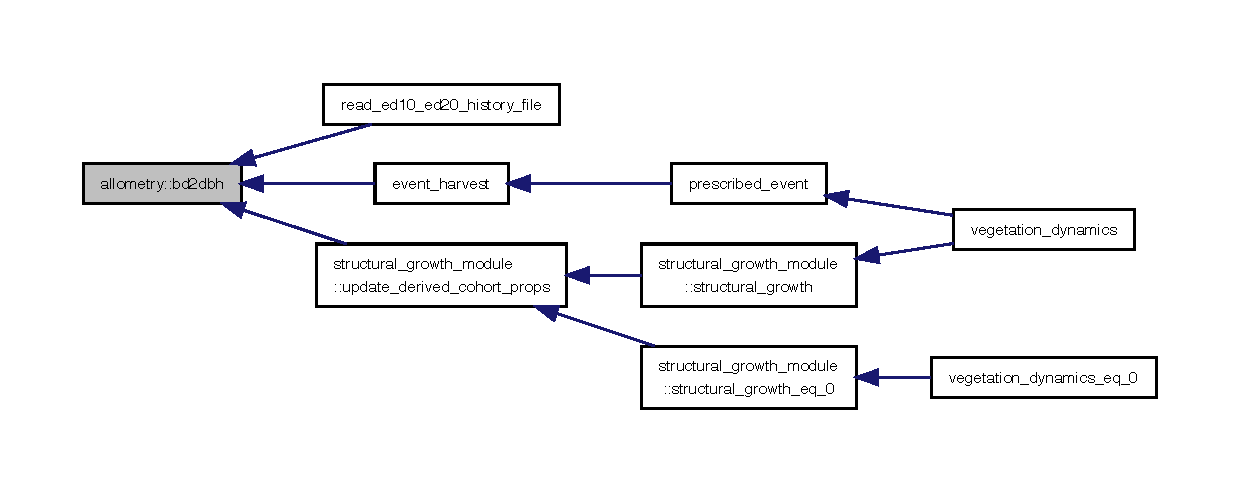
\includegraphics[width=350pt]{namespaceallometry_a50fedbee3a14eb5569a62abb4a36198f_icgraph}
\end{center}
\end{figure}
\mbox{\Hypertarget{namespaceallometry_a3236375dc165a26aeea2d97c7e2c2685}\label{namespaceallometry_a3236375dc165a26aeea2d97c7e2c2685}} 
\index{allometry@{allometry}!bl2dbh@{bl2dbh}}
\index{bl2dbh@{bl2dbh}!allometry@{allometry}}
\subsubsection{\texorpdfstring{bl2dbh()}{bl2dbh()}}
{\footnotesize\ttfamily real function allometry\+::bl2dbh (\begin{DoxyParamCaption}\item[{real, intent(in)}]{bleaf,  }\item[{integer, intent(in)}]{ipft }\end{DoxyParamCaption})}

Here is the call graph for this function\+:
\nopagebreak
\begin{figure}[H]
\begin{center}
\leavevmode
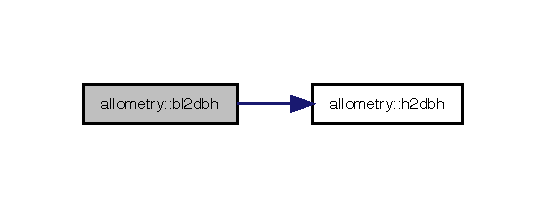
\includegraphics[width=262pt]{namespaceallometry_a3236375dc165a26aeea2d97c7e2c2685_cgraph}
\end{center}
\end{figure}
Here is the caller graph for this function\+:
\nopagebreak
\begin{figure}[H]
\begin{center}
\leavevmode
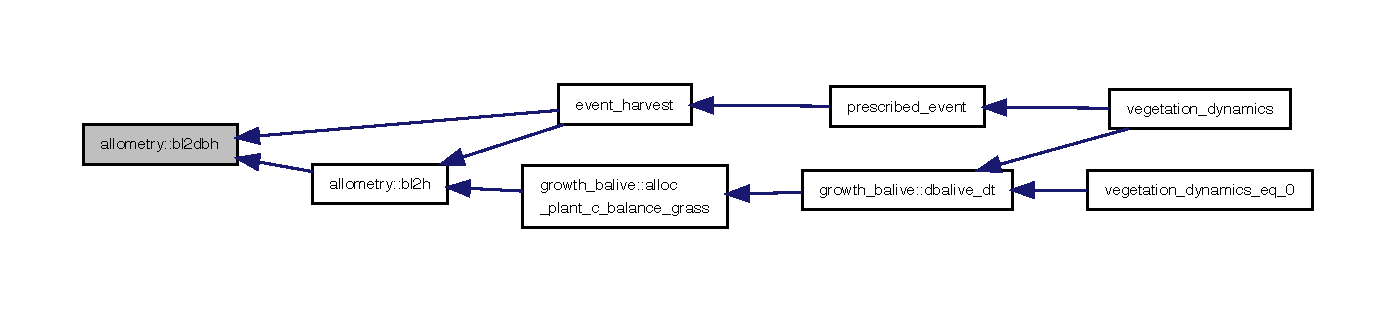
\includegraphics[width=350pt]{namespaceallometry_a3236375dc165a26aeea2d97c7e2c2685_icgraph}
\end{center}
\end{figure}
\mbox{\Hypertarget{namespaceallometry_a59a1fc10140498dee62fce8a641da254}\label{namespaceallometry_a59a1fc10140498dee62fce8a641da254}} 
\index{allometry@{allometry}!bl2h@{bl2h}}
\index{bl2h@{bl2h}!allometry@{allometry}}
\subsubsection{\texorpdfstring{bl2h()}{bl2h()}}
{\footnotesize\ttfamily real function allometry\+::bl2h (\begin{DoxyParamCaption}\item[{real, intent(in)}]{bleaf,  }\item[{integer, intent(in)}]{ipft }\end{DoxyParamCaption})}

Here is the call graph for this function\+:
\nopagebreak
\begin{figure}[H]
\begin{center}
\leavevmode
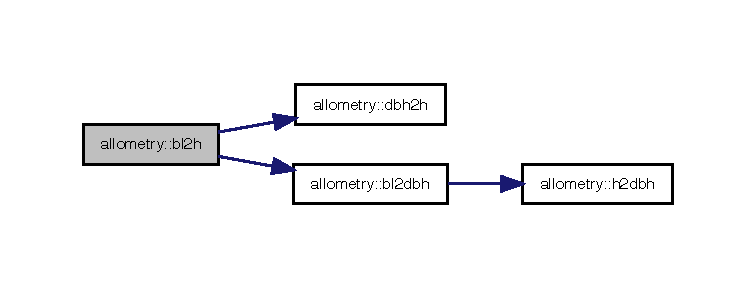
\includegraphics[width=350pt]{namespaceallometry_a59a1fc10140498dee62fce8a641da254_cgraph}
\end{center}
\end{figure}
Here is the caller graph for this function\+:
\nopagebreak
\begin{figure}[H]
\begin{center}
\leavevmode
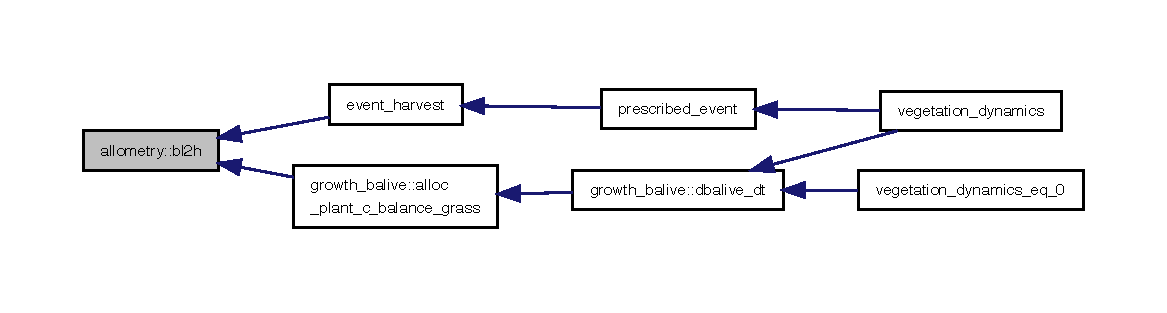
\includegraphics[width=350pt]{namespaceallometry_a59a1fc10140498dee62fce8a641da254_icgraph}
\end{center}
\end{figure}
\mbox{\Hypertarget{namespaceallometry_a76db2bc4aaa47db1e2656117ec476dba}\label{namespaceallometry_a76db2bc4aaa47db1e2656117ec476dba}} 
\index{allometry@{allometry}!dbh2bd@{dbh2bd}}
\index{dbh2bd@{dbh2bd}!allometry@{allometry}}
\subsubsection{\texorpdfstring{dbh2bd()}{dbh2bd()}}
{\footnotesize\ttfamily real function allometry\+::dbh2bd (\begin{DoxyParamCaption}\item[{real, intent(in)}]{dbh,  }\item[{integer, intent(in)}]{ipft }\end{DoxyParamCaption})}

Here is the caller graph for this function\+:
\nopagebreak
\begin{figure}[H]
\begin{center}
\leavevmode
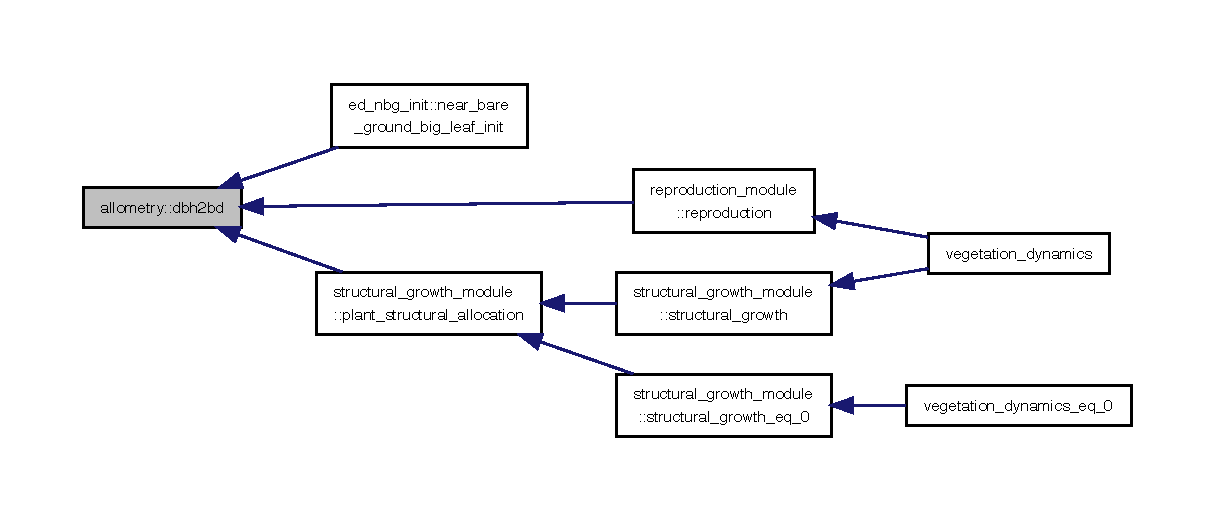
\includegraphics[width=350pt]{namespaceallometry_a76db2bc4aaa47db1e2656117ec476dba_icgraph}
\end{center}
\end{figure}
\mbox{\Hypertarget{namespaceallometry_abacdf8e8e585ce8d788a1fc2be133243}\label{namespaceallometry_abacdf8e8e585ce8d788a1fc2be133243}} 
\index{allometry@{allometry}!dbh2ca@{dbh2ca}}
\index{dbh2ca@{dbh2ca}!allometry@{allometry}}
\subsubsection{\texorpdfstring{dbh2ca()}{dbh2ca()}}
{\footnotesize\ttfamily real function allometry\+::dbh2ca (\begin{DoxyParamCaption}\item[{real, intent(in)}]{dbh,  }\item[{real, intent(in)}]{hite,  }\item[{real, intent(in)}]{sla,  }\item[{integer, intent(in)}]{ipft }\end{DoxyParamCaption})}

Here is the call graph for this function\+:
\nopagebreak
\begin{figure}[H]
\begin{center}
\leavevmode
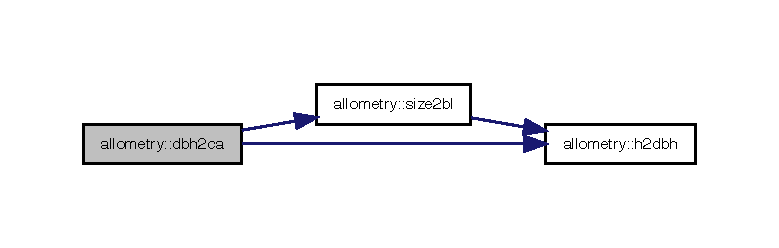
\includegraphics[width=350pt]{namespaceallometry_abacdf8e8e585ce8d788a1fc2be133243_cgraph}
\end{center}
\end{figure}
Here is the caller graph for this function\+:
\nopagebreak
\begin{figure}[H]
\begin{center}
\leavevmode
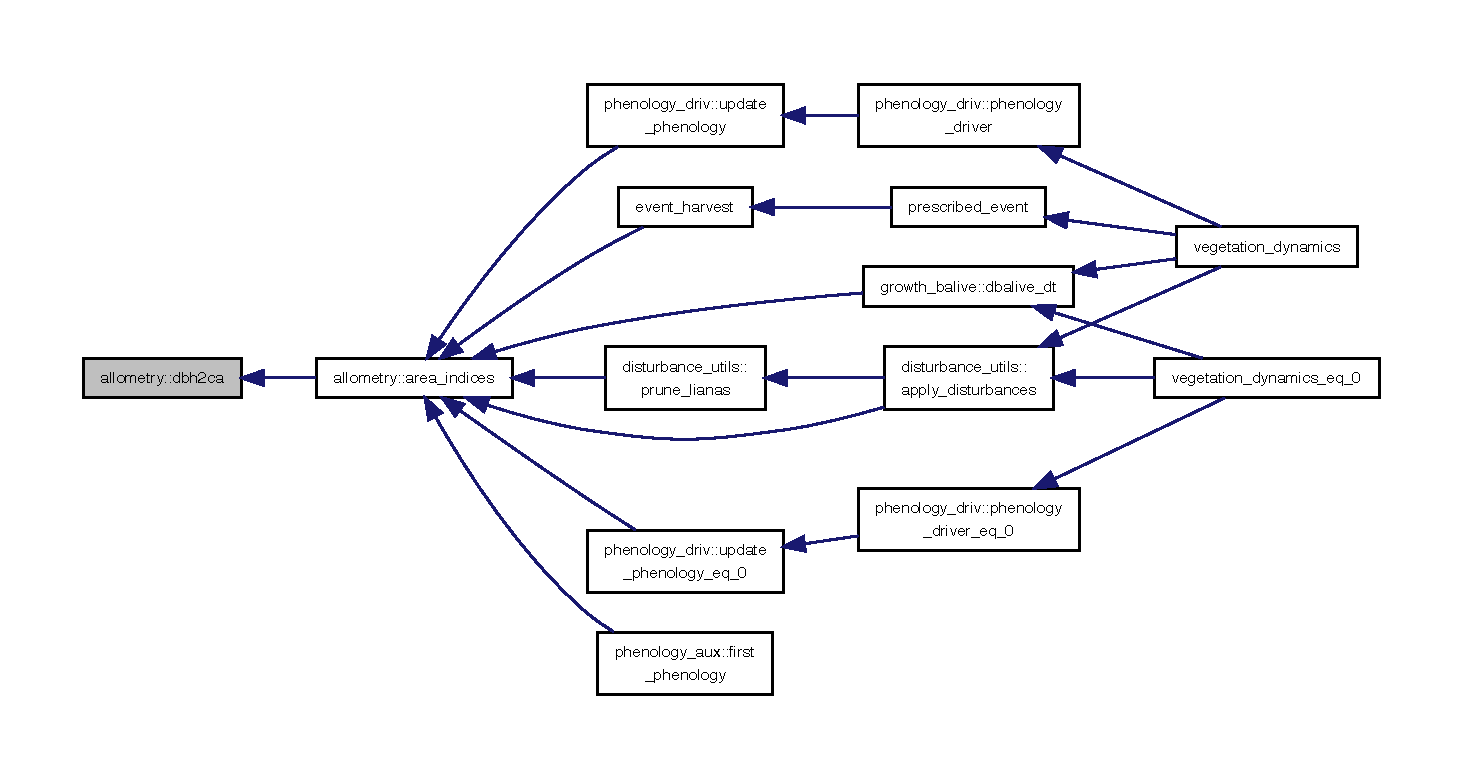
\includegraphics[width=350pt]{namespaceallometry_abacdf8e8e585ce8d788a1fc2be133243_icgraph}
\end{center}
\end{figure}
\mbox{\Hypertarget{namespaceallometry_a56f11dc07da4d5e7114dc37d6cc5f2cc}\label{namespaceallometry_a56f11dc07da4d5e7114dc37d6cc5f2cc}} 
\index{allometry@{allometry}!dbh2h@{dbh2h}}
\index{dbh2h@{dbh2h}!allometry@{allometry}}
\subsubsection{\texorpdfstring{dbh2h()}{dbh2h()}}
{\footnotesize\ttfamily real function allometry\+::dbh2h (\begin{DoxyParamCaption}\item[{integer, intent(in)}]{ipft,  }\item[{real, intent(in)}]{dbh }\end{DoxyParamCaption})}

Here is the caller graph for this function\+:
\nopagebreak
\begin{figure}[H]
\begin{center}
\leavevmode
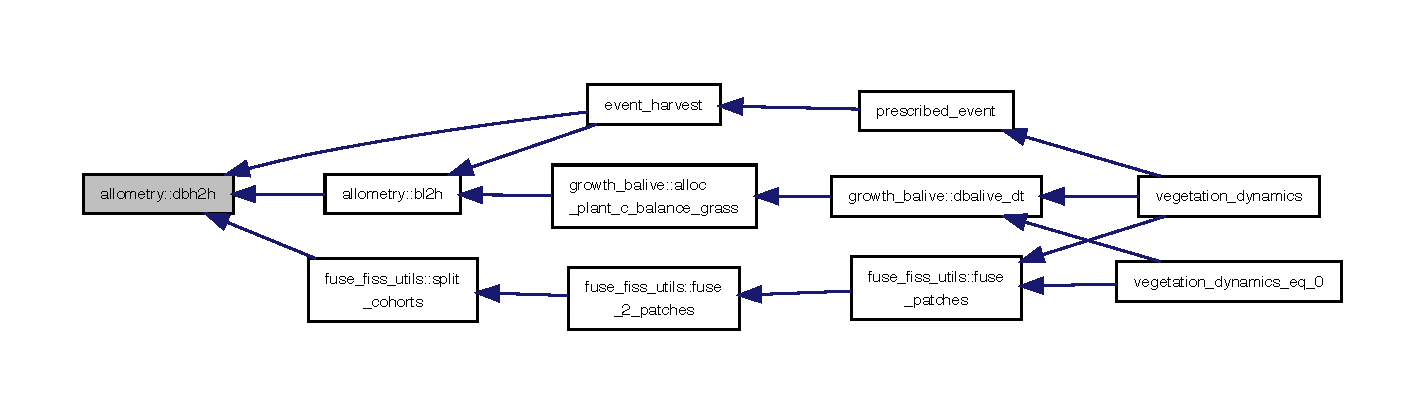
\includegraphics[width=350pt]{namespaceallometry_a56f11dc07da4d5e7114dc37d6cc5f2cc_icgraph}
\end{center}
\end{figure}
\mbox{\Hypertarget{namespaceallometry_ac1523ea0e0ef8d2dd6a429f61a013c1c}\label{namespaceallometry_ac1523ea0e0ef8d2dd6a429f61a013c1c}} 
\index{allometry@{allometry}!dbh2krdepth@{dbh2krdepth}}
\index{dbh2krdepth@{dbh2krdepth}!allometry@{allometry}}
\subsubsection{\texorpdfstring{dbh2krdepth()}{dbh2krdepth()}}
{\footnotesize\ttfamily integer function allometry\+::dbh2krdepth (\begin{DoxyParamCaption}\item[{real, intent(in)}]{hite,  }\item[{real, intent(in)}]{dbh,  }\item[{integer, intent(in)}]{ipft,  }\item[{integer, intent(in)}]{lsl }\end{DoxyParamCaption})}

Here is the call graph for this function\+:
\nopagebreak
\begin{figure}[H]
\begin{center}
\leavevmode
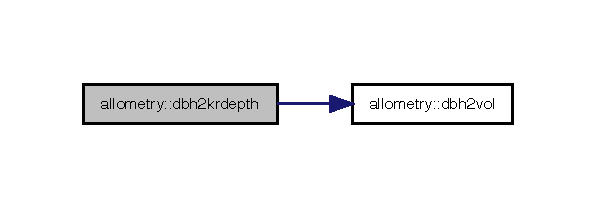
\includegraphics[width=286pt]{namespaceallometry_ac1523ea0e0ef8d2dd6a429f61a013c1c_cgraph}
\end{center}
\end{figure}
Here is the caller graph for this function\+:
\nopagebreak
\begin{figure}[H]
\begin{center}
\leavevmode
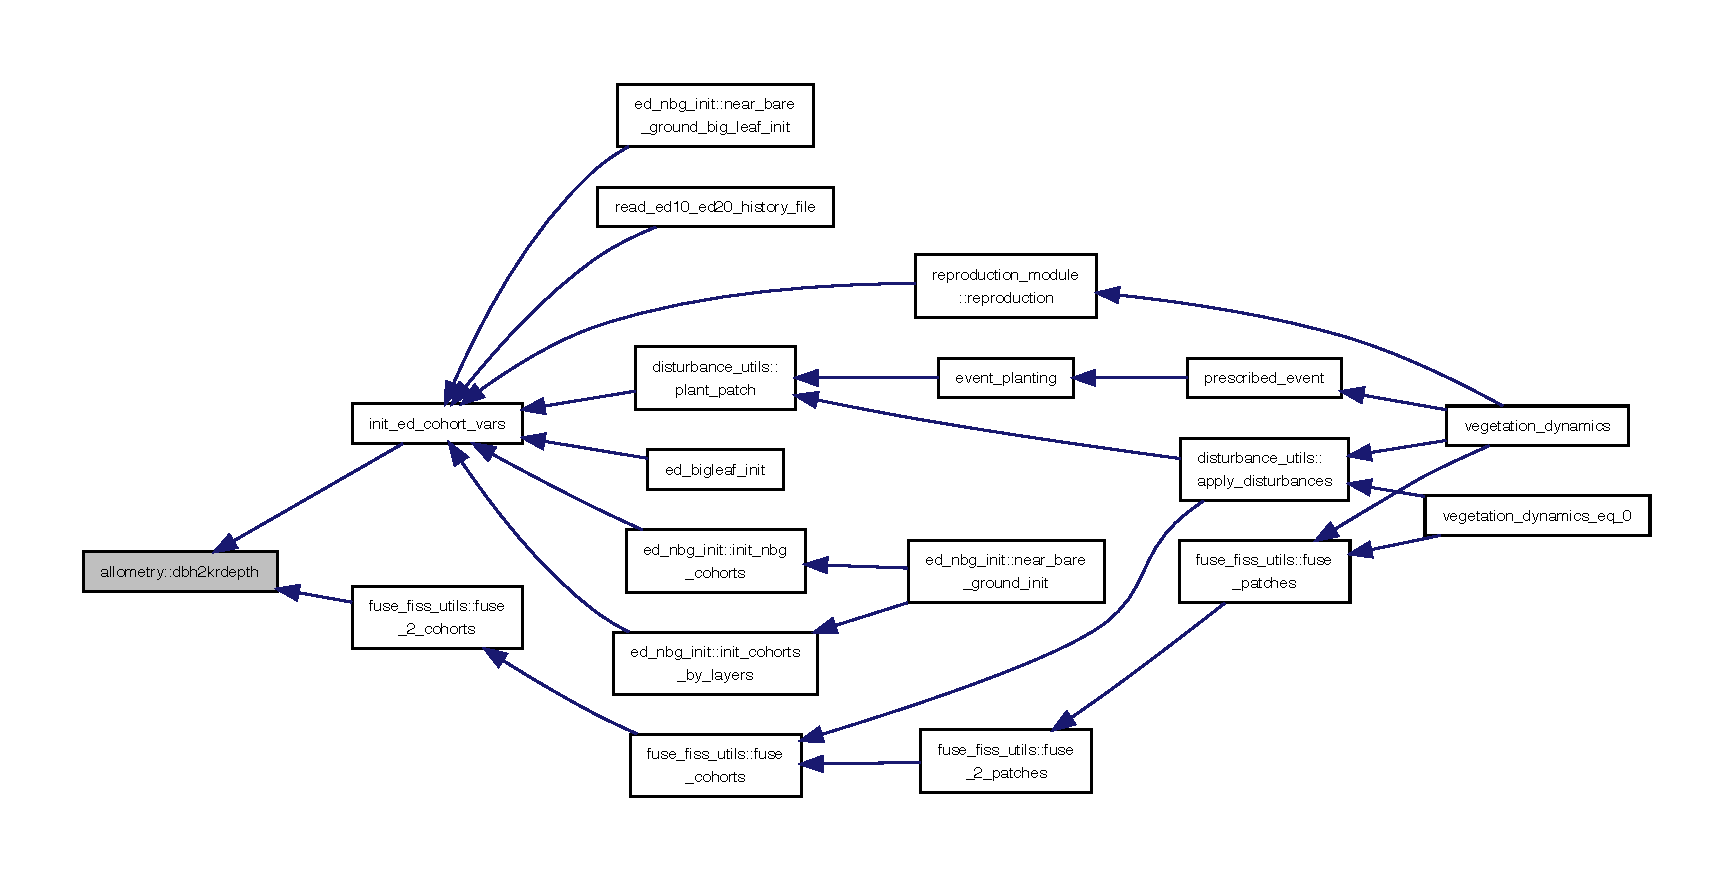
\includegraphics[width=350pt]{namespaceallometry_ac1523ea0e0ef8d2dd6a429f61a013c1c_icgraph}
\end{center}
\end{figure}
\mbox{\Hypertarget{namespaceallometry_aab2b2cee61cac31529246b043121c7de}\label{namespaceallometry_aab2b2cee61cac31529246b043121c7de}} 
\index{allometry@{allometry}!dbh2vol@{dbh2vol}}
\index{dbh2vol@{dbh2vol}!allometry@{allometry}}
\subsubsection{\texorpdfstring{dbh2vol()}{dbh2vol()}}
{\footnotesize\ttfamily real function allometry\+::dbh2vol (\begin{DoxyParamCaption}\item[{real, intent(in)}]{hgt,  }\item[{real, intent(in)}]{dbh,  }\item[{integer, intent(in)}]{ipft }\end{DoxyParamCaption})}

Here is the caller graph for this function\+:
\nopagebreak
\begin{figure}[H]
\begin{center}
\leavevmode
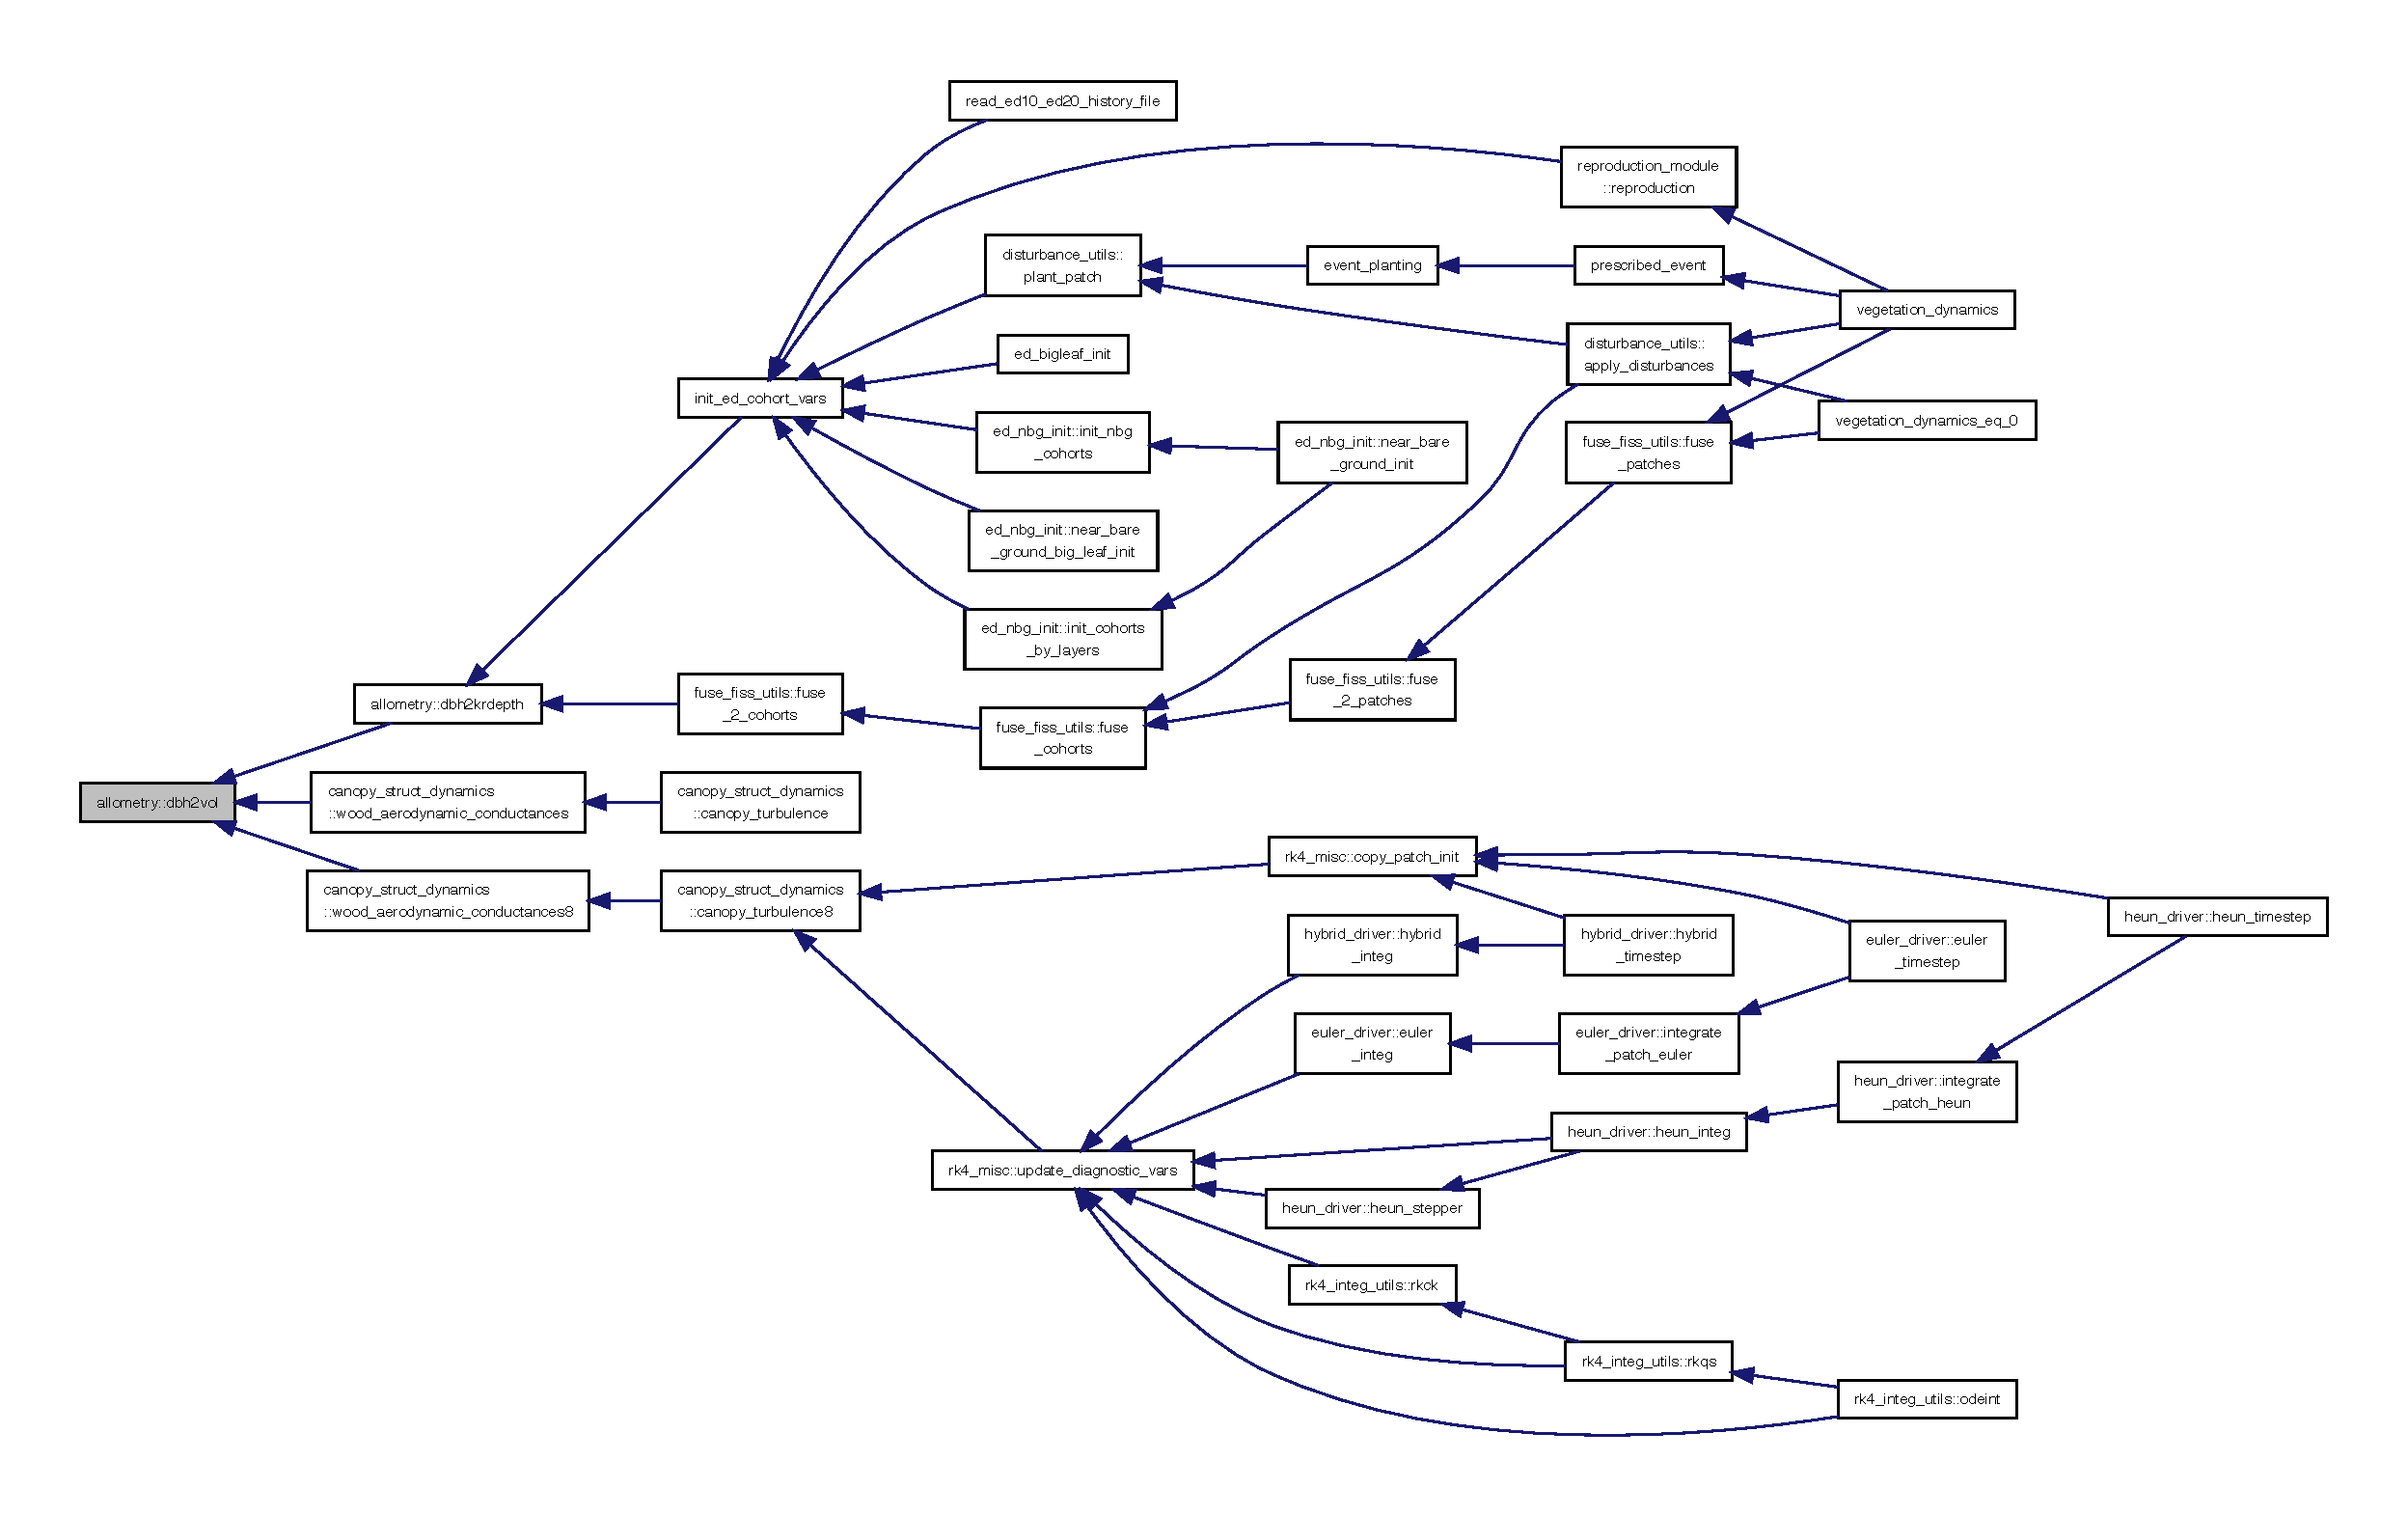
\includegraphics[width=350pt]{namespaceallometry_aab2b2cee61cac31529246b043121c7de_icgraph}
\end{center}
\end{figure}
\mbox{\Hypertarget{namespaceallometry_ab6a3d3302db0096b21354babe768677b}\label{namespaceallometry_ab6a3d3302db0096b21354babe768677b}} 
\index{allometry@{allometry}!ed\+\_\+biomass@{ed\+\_\+biomass}}
\index{ed\+\_\+biomass@{ed\+\_\+biomass}!allometry@{allometry}}
\subsubsection{\texorpdfstring{ed\+\_\+biomass()}{ed\_biomass()}}
{\footnotesize\ttfamily real function allometry\+::ed\+\_\+biomass (\begin{DoxyParamCaption}\item[{type(patchtype), target}]{cpatch,  }\item[{integer, intent(in)}]{ico }\end{DoxyParamCaption})}

Here is the caller graph for this function\+:
\nopagebreak
\begin{figure}[H]
\begin{center}
\leavevmode
\includegraphics[width=350pt]{namespaceallometry_ab6a3d3302db0096b21354babe768677b_icgraph}
\end{center}
\end{figure}
\mbox{\Hypertarget{namespaceallometry_a88949ed487fccc2f1dfd065399043b0d}\label{namespaceallometry_a88949ed487fccc2f1dfd065399043b0d}} 
\index{allometry@{allometry}!h2crownbh@{h2crownbh}}
\index{h2crownbh@{h2crownbh}!allometry@{allometry}}
\subsubsection{\texorpdfstring{h2crownbh()}{h2crownbh()}}
{\footnotesize\ttfamily real function allometry\+::h2crownbh (\begin{DoxyParamCaption}\item[{real, intent(in)}]{height,  }\item[{integer, intent(in)}]{ipft }\end{DoxyParamCaption})}

Here is the caller graph for this function\+:
\nopagebreak
\begin{figure}[H]
\begin{center}
\leavevmode
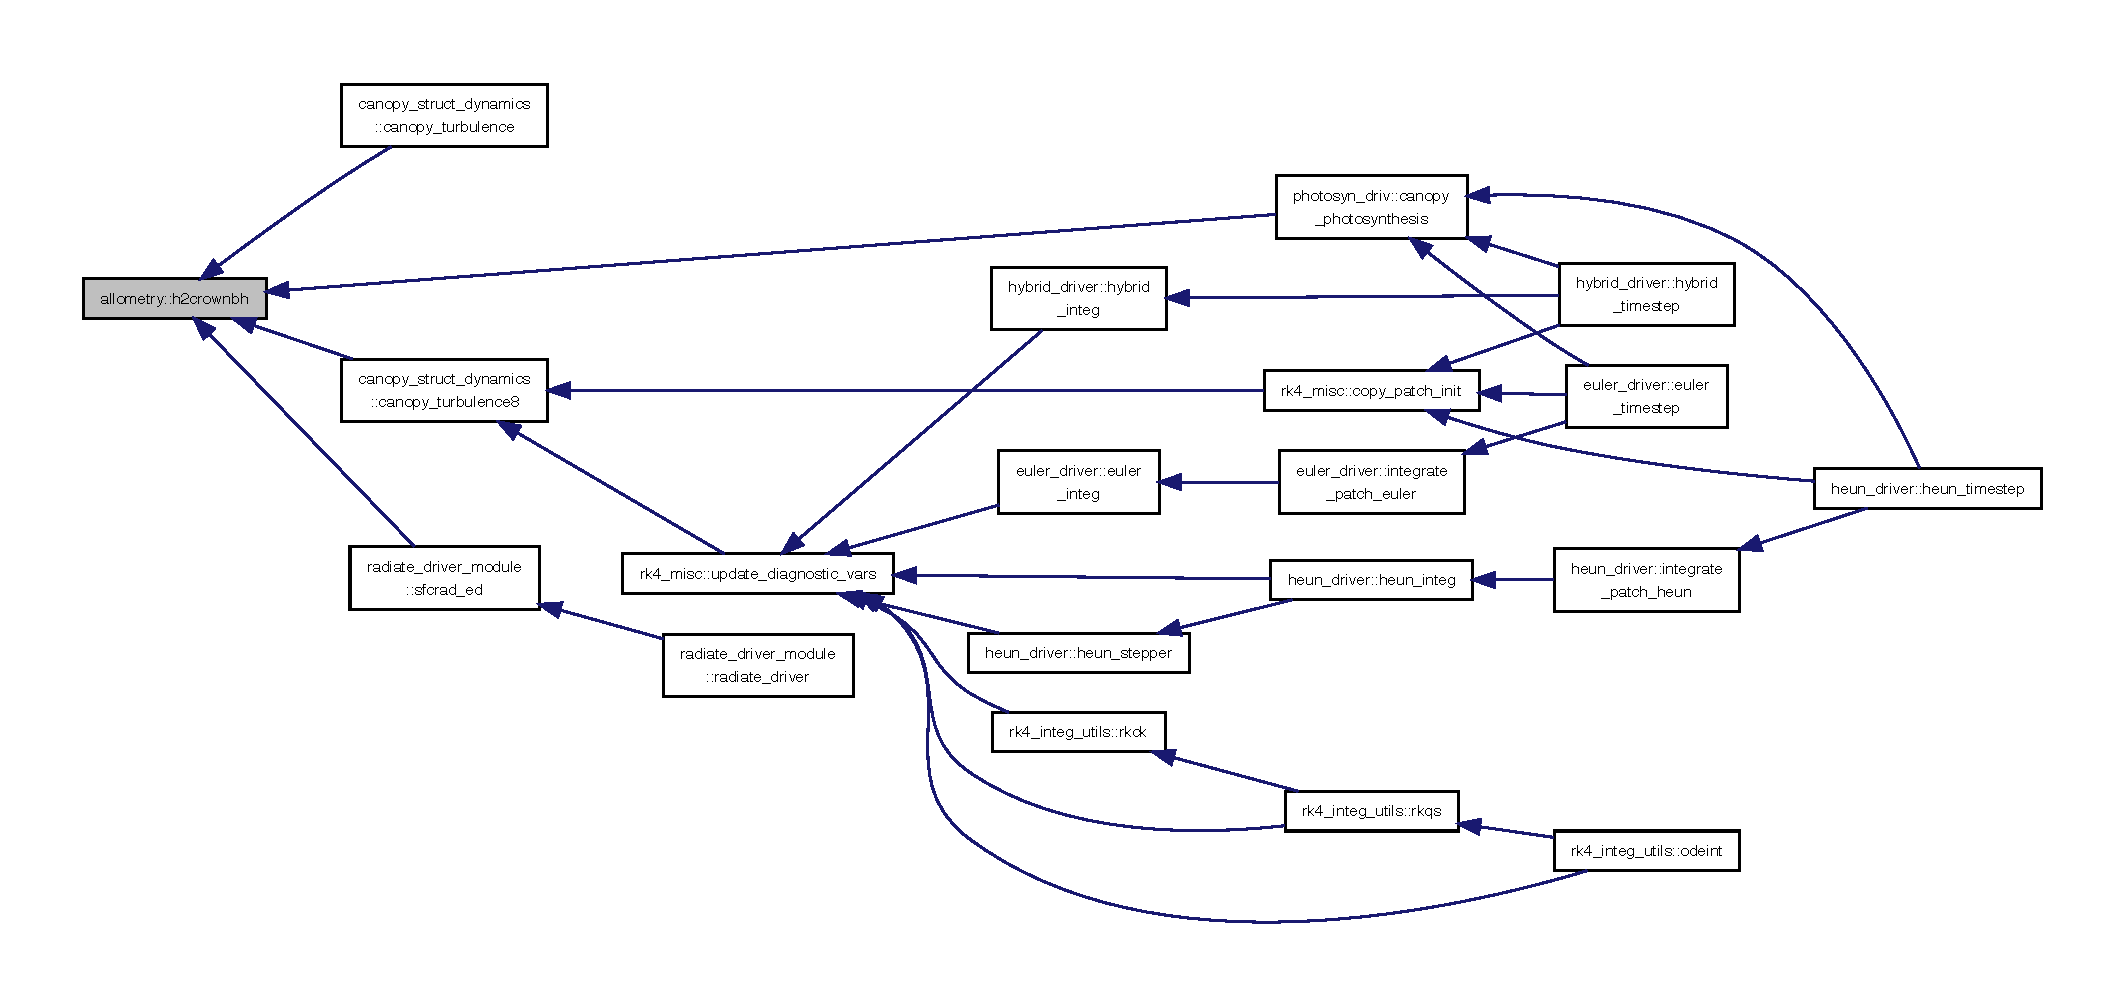
\includegraphics[width=350pt]{namespaceallometry_a88949ed487fccc2f1dfd065399043b0d_icgraph}
\end{center}
\end{figure}
\mbox{\Hypertarget{namespaceallometry_a31aa8db06e86ec74efb5e692417399df}\label{namespaceallometry_a31aa8db06e86ec74efb5e692417399df}} 
\index{allometry@{allometry}!h2dbh@{h2dbh}}
\index{h2dbh@{h2dbh}!allometry@{allometry}}
\subsubsection{\texorpdfstring{h2dbh()}{h2dbh()}}
{\footnotesize\ttfamily real function allometry\+::h2dbh (\begin{DoxyParamCaption}\item[{real, intent(in)}]{h,  }\item[{integer, intent(in)}]{ipft }\end{DoxyParamCaption})}

Here is the caller graph for this function\+:
\nopagebreak
\begin{figure}[H]
\begin{center}
\leavevmode
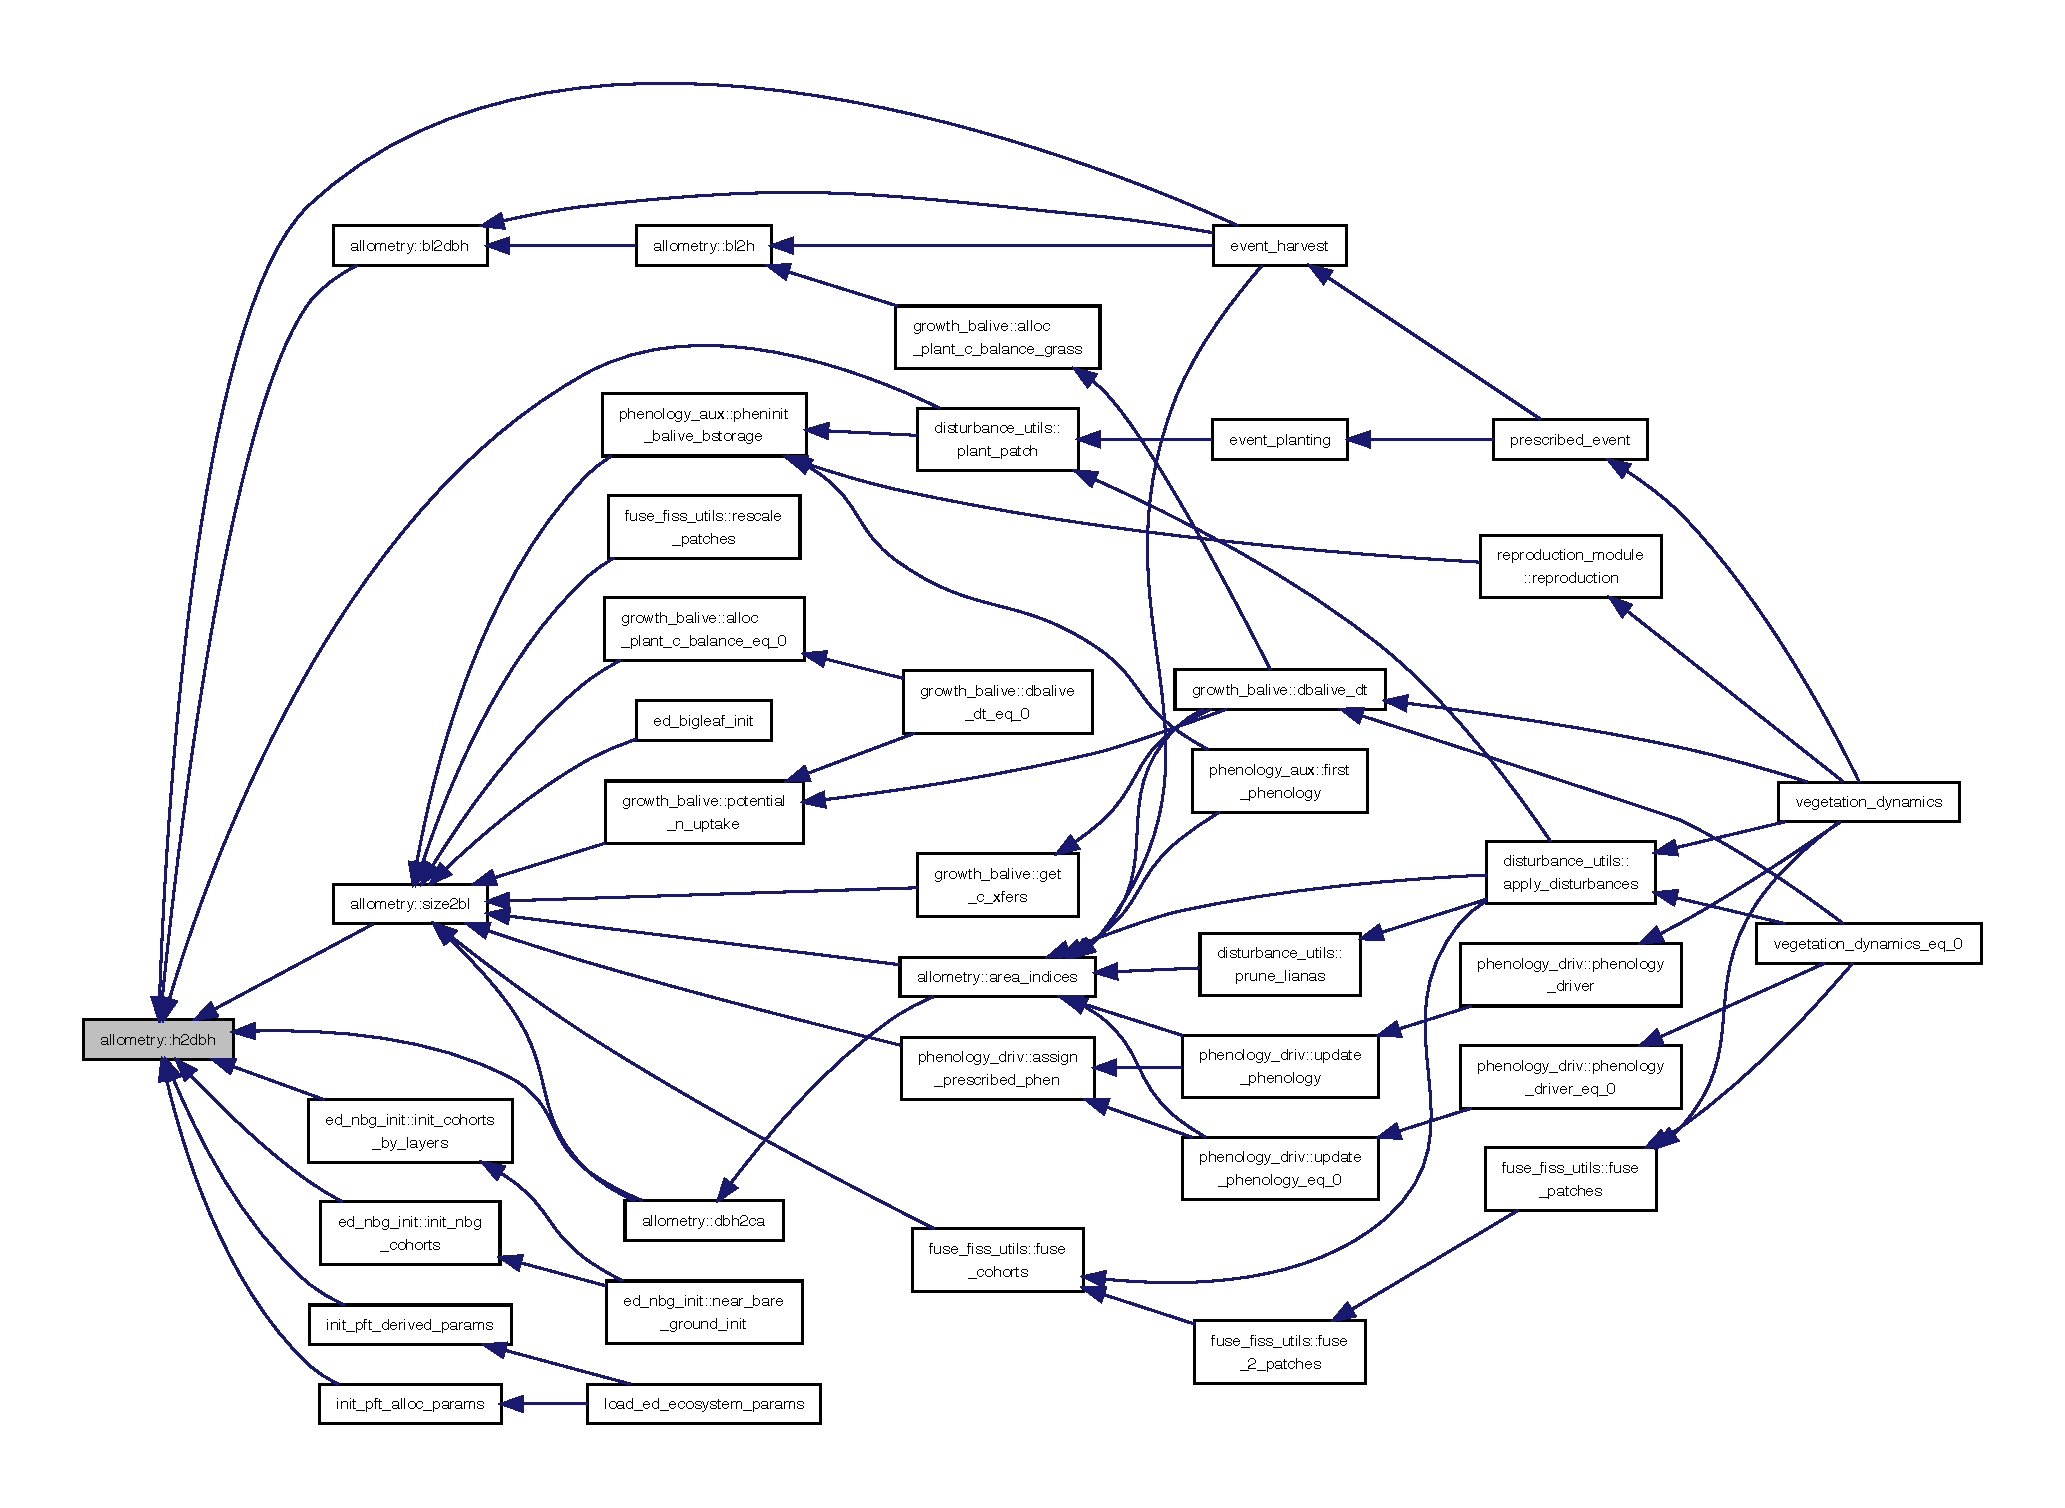
\includegraphics[width=350pt]{namespaceallometry_a31aa8db06e86ec74efb5e692417399df_icgraph}
\end{center}
\end{figure}
\mbox{\Hypertarget{namespaceallometry_a45ced9bf9ccd03debe8def35b579f4bd}\label{namespaceallometry_a45ced9bf9ccd03debe8def35b579f4bd}} 
\index{allometry@{allometry}!size2bl@{size2bl}}
\index{size2bl@{size2bl}!allometry@{allometry}}
\subsubsection{\texorpdfstring{size2bl()}{size2bl()}}
{\footnotesize\ttfamily real function allometry\+::size2bl (\begin{DoxyParamCaption}\item[{real, intent(in)}]{dbh,  }\item[{real, intent(in)}]{hite,  }\item[{integer, intent(in)}]{ipft }\end{DoxyParamCaption})}

Here is the call graph for this function\+:
\nopagebreak
\begin{figure}[H]
\begin{center}
\leavevmode
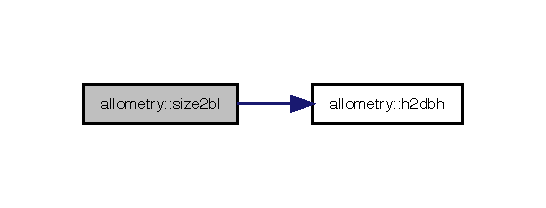
\includegraphics[width=262pt]{namespaceallometry_a45ced9bf9ccd03debe8def35b579f4bd_cgraph}
\end{center}
\end{figure}
Here is the caller graph for this function\+:
\nopagebreak
\begin{figure}[H]
\begin{center}
\leavevmode
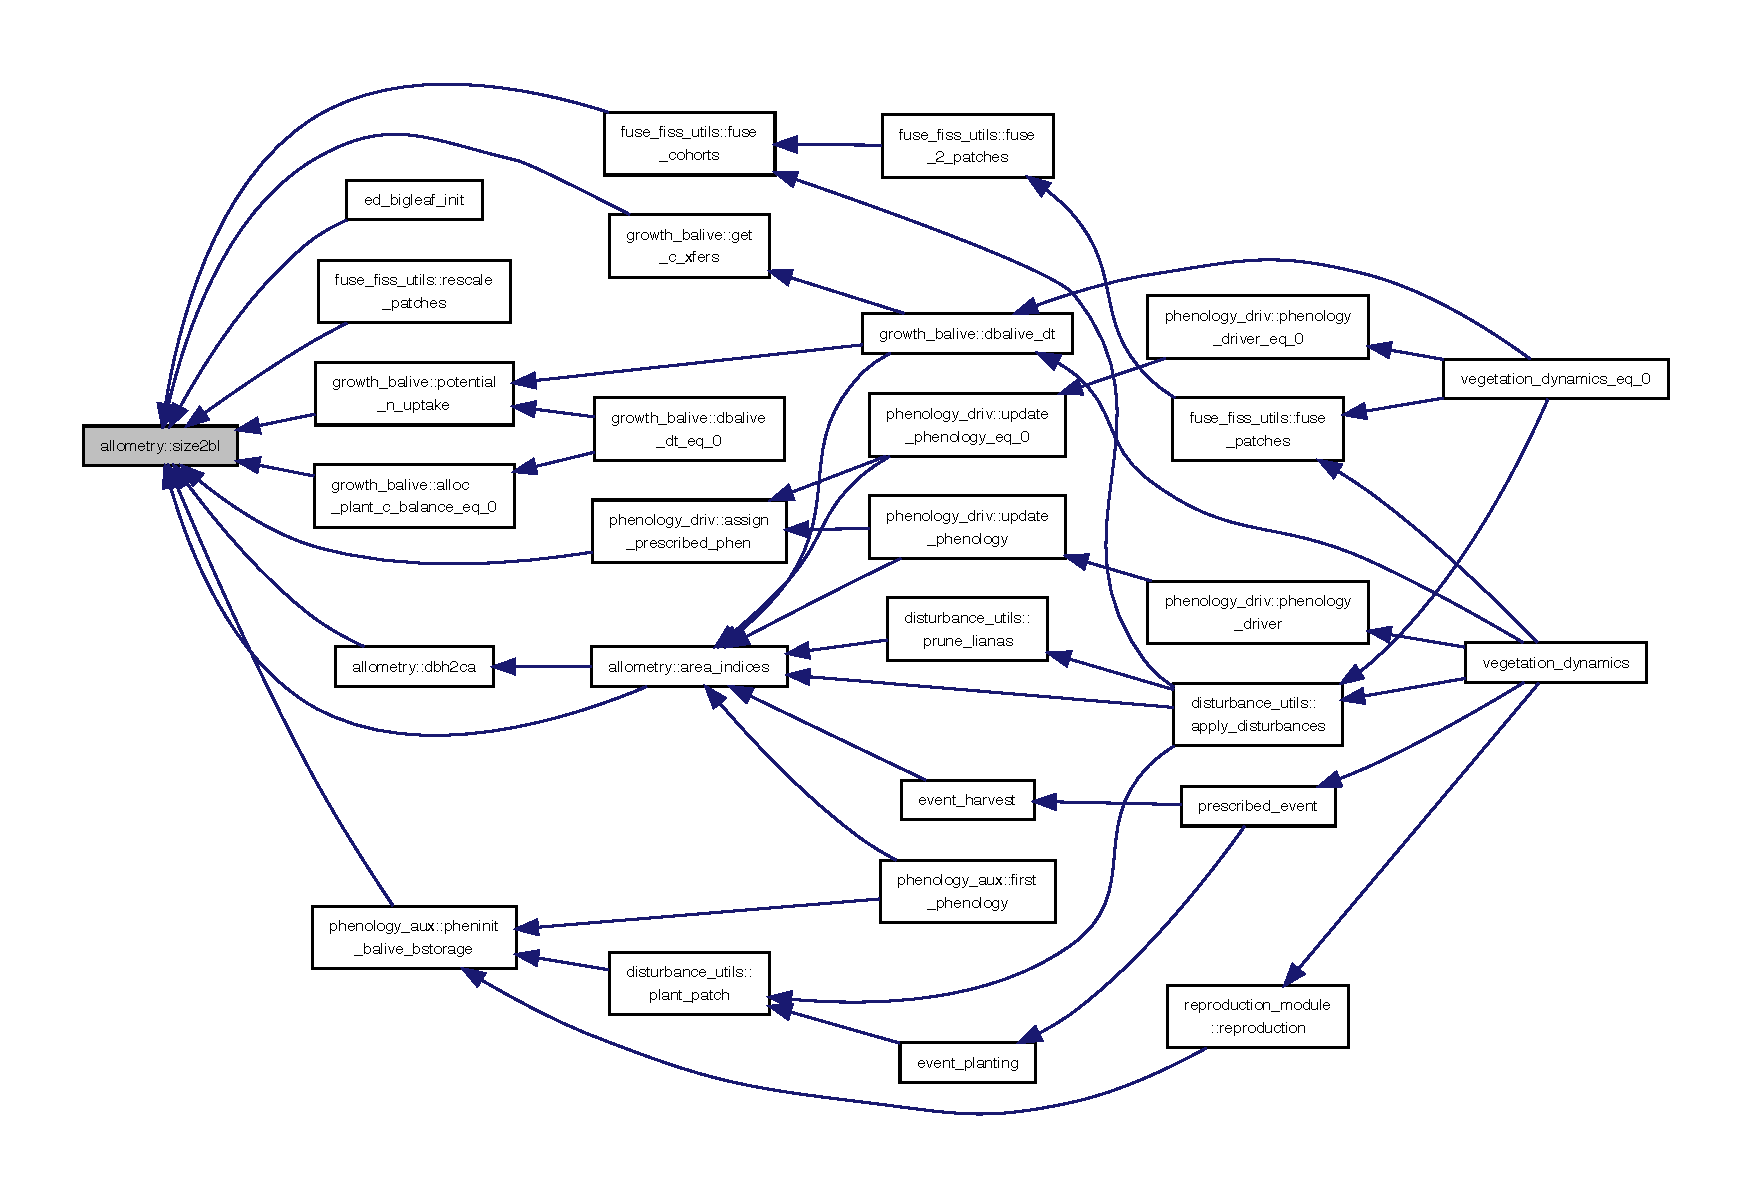
\includegraphics[width=350pt]{namespaceallometry_a45ced9bf9ccd03debe8def35b579f4bd_icgraph}
\end{center}
\end{figure}

\hypertarget{namespacean__header}{}\section{an\+\_\+header Module Reference}
\label{namespacean__header}\index{an\+\_\+header@{an\+\_\+header}}
\subsection*{Data Types}
\begin{DoxyCompactItemize}
\item 
type \hyperlink{structan__header_1_1head__table}{head\+\_\+table}
\end{DoxyCompactItemize}
\subsection*{Variables}
\begin{DoxyCompactItemize}
\item 
type(\hyperlink{structan__header_1_1head__table}{head\+\_\+table}), dimension(\+:), allocatable, save \hyperlink{namespacean__header_ae5d3cd005b4f936e39d8ca9572fad953}{anal\+\_\+table}
\item 
integer, save \hyperlink{namespacean__header_a1f6702c906713337344986a86e036d55}{nvbtab}
\end{DoxyCompactItemize}


\subsection{Variable Documentation}
\mbox{\Hypertarget{namespacean__header_ae5d3cd005b4f936e39d8ca9572fad953}\label{namespacean__header_ae5d3cd005b4f936e39d8ca9572fad953}} 
\index{an\+\_\+header@{an\+\_\+header}!anal\+\_\+table@{anal\+\_\+table}}
\index{anal\+\_\+table@{anal\+\_\+table}!an\+\_\+header@{an\+\_\+header}}
\subsubsection{\texorpdfstring{anal\+\_\+table}{anal\_table}}
{\footnotesize\ttfamily type (\hyperlink{structan__header_1_1head__table}{head\+\_\+table}), dimension(\+:), allocatable, save an\+\_\+header\+::anal\+\_\+table}

\mbox{\Hypertarget{namespacean__header_a1f6702c906713337344986a86e036d55}\label{namespacean__header_a1f6702c906713337344986a86e036d55}} 
\index{an\+\_\+header@{an\+\_\+header}!nvbtab@{nvbtab}}
\index{nvbtab@{nvbtab}!an\+\_\+header@{an\+\_\+header}}
\subsubsection{\texorpdfstring{nvbtab}{nvbtab}}
{\footnotesize\ttfamily integer, save an\+\_\+header\+::nvbtab}


\hypertarget{namespaceaverage__utils}{}\section{average\+\_\+utils Module Reference}
\label{namespaceaverage__utils}\index{average\+\_\+utils@{average\+\_\+utils}}
\subsection*{Functions/\+Subroutines}
\begin{DoxyCompactItemize}
\item 
subroutine \hyperlink{namespaceaverage__utils_a90965230835c19a82d90127089235c76}{aggregate\+\_\+polygon\+\_\+fmean} (cgrid)
\item 
subroutine \hyperlink{namespaceaverage__utils_acf7868319b9242daa7eea553b25f2899}{integrate\+\_\+ed\+\_\+fmean\+\_\+met\+\_\+vars} (cgrid)
\item 
subroutine \hyperlink{namespaceaverage__utils_a662a31926be61beb22be003b5ec40343}{normalize\+\_\+ed\+\_\+fmean\+\_\+vars} (cgrid)
\item 
subroutine \hyperlink{namespaceaverage__utils_a40f7a4a46972fb6b9c0fe90fdc73a173}{zero\+\_\+ed\+\_\+fmean\+\_\+vars} (cgrid)
\item 
subroutine \hyperlink{namespaceaverage__utils_a985b401d85dd857f44371dd2c3e7c40c}{integrate\+\_\+ed\+\_\+dmean\+\_\+vars} (cgrid)
\item 
subroutine \hyperlink{namespaceaverage__utils_a538e2e59c7c2889ae624b6e1d2a9e5f2}{normalize\+\_\+ed\+\_\+today\+\_\+vars} (cgrid)
\item 
subroutine \hyperlink{namespaceaverage__utils_a446f9090fbbcf3eb12f4b9231d946e89}{normalize\+\_\+ed\+\_\+todaynpp\+\_\+vars} (cgrid)
\item 
subroutine \hyperlink{namespaceaverage__utils_a2203ebc403bfd01a55cf7aac61777819}{normalize\+\_\+ed\+\_\+dmean\+\_\+vars} (cgrid)
\item 
subroutine \hyperlink{namespaceaverage__utils_a6a92d00bf7112b127a596bd765cc12c6}{zero\+\_\+ed\+\_\+today\+\_\+vars} (cgrid)
\item 
subroutine \hyperlink{namespaceaverage__utils_af1a2224da3c590c5645db8efa5c16c9f}{zero\+\_\+ed\+\_\+dmean\+\_\+vars} (cgrid)
\item 
subroutine \hyperlink{namespaceaverage__utils_a24f0cd542ec9741c1bcc76e640498cd2}{integrate\+\_\+ed\+\_\+mmean\+\_\+vars} (cgrid)
\item 
subroutine \hyperlink{namespaceaverage__utils_afce18c59b2e9d5605d22e4d356934bdb}{normalize\+\_\+ed\+\_\+mmean\+\_\+vars} (cgrid)
\item 
subroutine \hyperlink{namespaceaverage__utils_aa5221fd3b377dfe424dbdcb81b83c378}{zero\+\_\+ed\+\_\+mmean\+\_\+vars} (cgrid)
\item 
subroutine \hyperlink{namespaceaverage__utils_af429d166f6097c18d6ab4ce05adbd31f}{integrate\+\_\+ed\+\_\+qmean\+\_\+vars} (cgrid)
\item 
subroutine \hyperlink{namespaceaverage__utils_ad7f232f9a24079c3430b005098729615}{normalize\+\_\+ed\+\_\+qmean\+\_\+vars} (cgrid)
\item 
subroutine \hyperlink{namespaceaverage__utils_a2e9cb2592327099345c147516b927f51}{zero\+\_\+ed\+\_\+qmean\+\_\+vars} (cgrid)
\item 
subroutine \hyperlink{namespaceaverage__utils_a81384775dd05dba144bf83e9731d5275}{update\+\_\+ed\+\_\+yearly\+\_\+vars} (cgrid)
\item 
subroutine \hyperlink{namespaceaverage__utils_a81df7cc84b1d62f7fb950e91d410abbd}{zero\+\_\+ed\+\_\+yearly\+\_\+vars} (cgrid)
\item 
real(kind=4) function \hyperlink{namespaceaverage__utils_ac90817fe39c27153ed7bbee2cb856611}{isqu\+\_\+ftz} (x)
\end{DoxyCompactItemize}


\subsection{Function/\+Subroutine Documentation}
\mbox{\Hypertarget{namespaceaverage__utils_a90965230835c19a82d90127089235c76}\label{namespaceaverage__utils_a90965230835c19a82d90127089235c76}} 
\index{average\+\_\+utils@{average\+\_\+utils}!aggregate\+\_\+polygon\+\_\+fmean@{aggregate\+\_\+polygon\+\_\+fmean}}
\index{aggregate\+\_\+polygon\+\_\+fmean@{aggregate\+\_\+polygon\+\_\+fmean}!average\+\_\+utils@{average\+\_\+utils}}
\subsubsection{\texorpdfstring{aggregate\+\_\+polygon\+\_\+fmean()}{aggregate\_polygon\_fmean()}}
{\footnotesize\ttfamily subroutine average\+\_\+utils\+::aggregate\+\_\+polygon\+\_\+fmean (\begin{DoxyParamCaption}\item[{type(edtype), target}]{cgrid }\end{DoxyParamCaption})}

Here is the call graph for this function\+:
\nopagebreak
\begin{figure}[H]
\begin{center}
\leavevmode
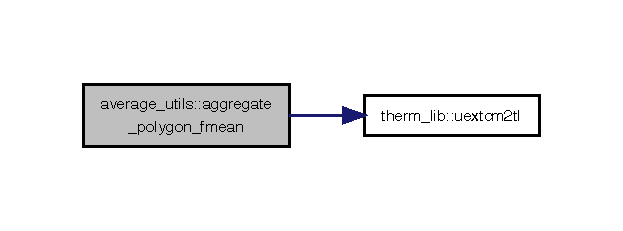
\includegraphics[width=299pt]{namespaceaverage__utils_a90965230835c19a82d90127089235c76_cgraph}
\end{center}
\end{figure}
Here is the caller graph for this function\+:
\nopagebreak
\begin{figure}[H]
\begin{center}
\leavevmode
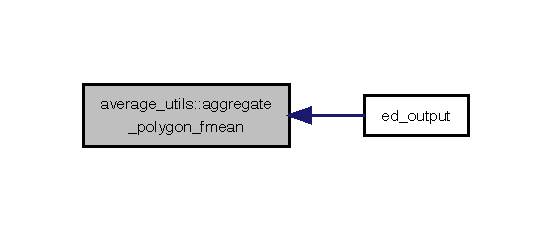
\includegraphics[width=265pt]{namespaceaverage__utils_a90965230835c19a82d90127089235c76_icgraph}
\end{center}
\end{figure}
\mbox{\Hypertarget{namespaceaverage__utils_a985b401d85dd857f44371dd2c3e7c40c}\label{namespaceaverage__utils_a985b401d85dd857f44371dd2c3e7c40c}} 
\index{average\+\_\+utils@{average\+\_\+utils}!integrate\+\_\+ed\+\_\+dmean\+\_\+vars@{integrate\+\_\+ed\+\_\+dmean\+\_\+vars}}
\index{integrate\+\_\+ed\+\_\+dmean\+\_\+vars@{integrate\+\_\+ed\+\_\+dmean\+\_\+vars}!average\+\_\+utils@{average\+\_\+utils}}
\subsubsection{\texorpdfstring{integrate\+\_\+ed\+\_\+dmean\+\_\+vars()}{integrate\_ed\_dmean\_vars()}}
{\footnotesize\ttfamily subroutine average\+\_\+utils\+::integrate\+\_\+ed\+\_\+dmean\+\_\+vars (\begin{DoxyParamCaption}\item[{type(edtype), target}]{cgrid }\end{DoxyParamCaption})}

\mbox{\Hypertarget{namespaceaverage__utils_acf7868319b9242daa7eea553b25f2899}\label{namespaceaverage__utils_acf7868319b9242daa7eea553b25f2899}} 
\index{average\+\_\+utils@{average\+\_\+utils}!integrate\+\_\+ed\+\_\+fmean\+\_\+met\+\_\+vars@{integrate\+\_\+ed\+\_\+fmean\+\_\+met\+\_\+vars}}
\index{integrate\+\_\+ed\+\_\+fmean\+\_\+met\+\_\+vars@{integrate\+\_\+ed\+\_\+fmean\+\_\+met\+\_\+vars}!average\+\_\+utils@{average\+\_\+utils}}
\subsubsection{\texorpdfstring{integrate\+\_\+ed\+\_\+fmean\+\_\+met\+\_\+vars()}{integrate\_ed\_fmean\_met\_vars()}}
{\footnotesize\ttfamily subroutine average\+\_\+utils\+::integrate\+\_\+ed\+\_\+fmean\+\_\+met\+\_\+vars (\begin{DoxyParamCaption}\item[{type(edtype), target}]{cgrid }\end{DoxyParamCaption})}

\mbox{\Hypertarget{namespaceaverage__utils_a24f0cd542ec9741c1bcc76e640498cd2}\label{namespaceaverage__utils_a24f0cd542ec9741c1bcc76e640498cd2}} 
\index{average\+\_\+utils@{average\+\_\+utils}!integrate\+\_\+ed\+\_\+mmean\+\_\+vars@{integrate\+\_\+ed\+\_\+mmean\+\_\+vars}}
\index{integrate\+\_\+ed\+\_\+mmean\+\_\+vars@{integrate\+\_\+ed\+\_\+mmean\+\_\+vars}!average\+\_\+utils@{average\+\_\+utils}}
\subsubsection{\texorpdfstring{integrate\+\_\+ed\+\_\+mmean\+\_\+vars()}{integrate\_ed\_mmean\_vars()}}
{\footnotesize\ttfamily subroutine average\+\_\+utils\+::integrate\+\_\+ed\+\_\+mmean\+\_\+vars (\begin{DoxyParamCaption}\item[{type(edtype), target}]{cgrid }\end{DoxyParamCaption})}

Here is the call graph for this function\+:
\nopagebreak
\begin{figure}[H]
\begin{center}
\leavevmode
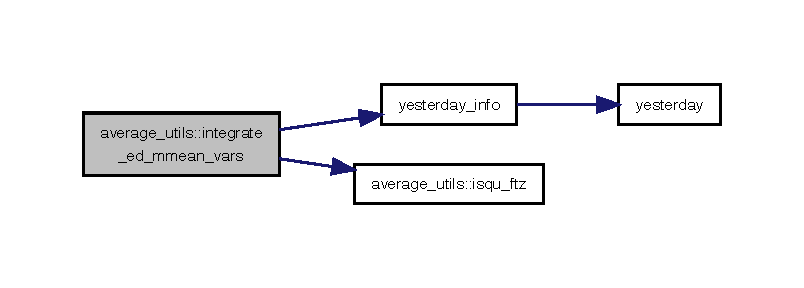
\includegraphics[width=350pt]{namespaceaverage__utils_a24f0cd542ec9741c1bcc76e640498cd2_cgraph}
\end{center}
\end{figure}
\mbox{\Hypertarget{namespaceaverage__utils_af429d166f6097c18d6ab4ce05adbd31f}\label{namespaceaverage__utils_af429d166f6097c18d6ab4ce05adbd31f}} 
\index{average\+\_\+utils@{average\+\_\+utils}!integrate\+\_\+ed\+\_\+qmean\+\_\+vars@{integrate\+\_\+ed\+\_\+qmean\+\_\+vars}}
\index{integrate\+\_\+ed\+\_\+qmean\+\_\+vars@{integrate\+\_\+ed\+\_\+qmean\+\_\+vars}!average\+\_\+utils@{average\+\_\+utils}}
\subsubsection{\texorpdfstring{integrate\+\_\+ed\+\_\+qmean\+\_\+vars()}{integrate\_ed\_qmean\_vars()}}
{\footnotesize\ttfamily subroutine average\+\_\+utils\+::integrate\+\_\+ed\+\_\+qmean\+\_\+vars (\begin{DoxyParamCaption}\item[{type(edtype), target}]{cgrid }\end{DoxyParamCaption})}

Here is the call graph for this function\+:
\nopagebreak
\begin{figure}[H]
\begin{center}
\leavevmode
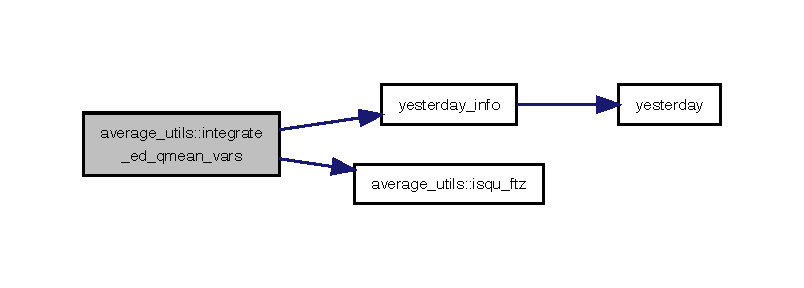
\includegraphics[width=350pt]{namespaceaverage__utils_af429d166f6097c18d6ab4ce05adbd31f_cgraph}
\end{center}
\end{figure}
\mbox{\Hypertarget{namespaceaverage__utils_ac90817fe39c27153ed7bbee2cb856611}\label{namespaceaverage__utils_ac90817fe39c27153ed7bbee2cb856611}} 
\index{average\+\_\+utils@{average\+\_\+utils}!isqu\+\_\+ftz@{isqu\+\_\+ftz}}
\index{isqu\+\_\+ftz@{isqu\+\_\+ftz}!average\+\_\+utils@{average\+\_\+utils}}
\subsubsection{\texorpdfstring{isqu\+\_\+ftz()}{isqu\_ftz()}}
{\footnotesize\ttfamily real(kind=4) function average\+\_\+utils\+::isqu\+\_\+ftz (\begin{DoxyParamCaption}\item[{real(kind=4), intent(in)}]{x }\end{DoxyParamCaption})}

Here is the caller graph for this function\+:
\nopagebreak
\begin{figure}[H]
\begin{center}
\leavevmode
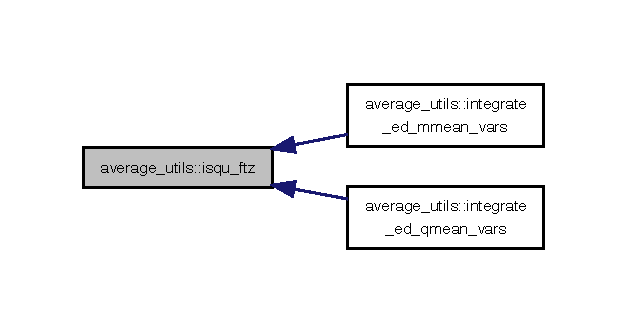
\includegraphics[width=301pt]{namespaceaverage__utils_ac90817fe39c27153ed7bbee2cb856611_icgraph}
\end{center}
\end{figure}
\mbox{\Hypertarget{namespaceaverage__utils_a2203ebc403bfd01a55cf7aac61777819}\label{namespaceaverage__utils_a2203ebc403bfd01a55cf7aac61777819}} 
\index{average\+\_\+utils@{average\+\_\+utils}!normalize\+\_\+ed\+\_\+dmean\+\_\+vars@{normalize\+\_\+ed\+\_\+dmean\+\_\+vars}}
\index{normalize\+\_\+ed\+\_\+dmean\+\_\+vars@{normalize\+\_\+ed\+\_\+dmean\+\_\+vars}!average\+\_\+utils@{average\+\_\+utils}}
\subsubsection{\texorpdfstring{normalize\+\_\+ed\+\_\+dmean\+\_\+vars()}{normalize\_ed\_dmean\_vars()}}
{\footnotesize\ttfamily subroutine average\+\_\+utils\+::normalize\+\_\+ed\+\_\+dmean\+\_\+vars (\begin{DoxyParamCaption}\item[{type(edtype), target}]{cgrid }\end{DoxyParamCaption})}

Here is the call graph for this function\+:
\nopagebreak
\begin{figure}[H]
\begin{center}
\leavevmode
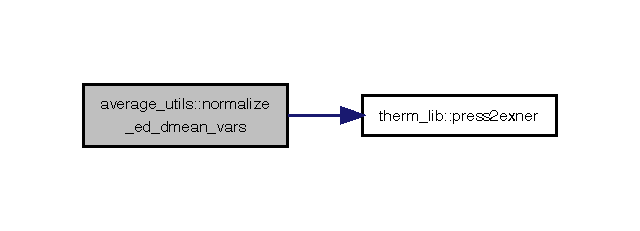
\includegraphics[width=307pt]{namespaceaverage__utils_a2203ebc403bfd01a55cf7aac61777819_cgraph}
\end{center}
\end{figure}
\mbox{\Hypertarget{namespaceaverage__utils_a662a31926be61beb22be003b5ec40343}\label{namespaceaverage__utils_a662a31926be61beb22be003b5ec40343}} 
\index{average\+\_\+utils@{average\+\_\+utils}!normalize\+\_\+ed\+\_\+fmean\+\_\+vars@{normalize\+\_\+ed\+\_\+fmean\+\_\+vars}}
\index{normalize\+\_\+ed\+\_\+fmean\+\_\+vars@{normalize\+\_\+ed\+\_\+fmean\+\_\+vars}!average\+\_\+utils@{average\+\_\+utils}}
\subsubsection{\texorpdfstring{normalize\+\_\+ed\+\_\+fmean\+\_\+vars()}{normalize\_ed\_fmean\_vars()}}
{\footnotesize\ttfamily subroutine average\+\_\+utils\+::normalize\+\_\+ed\+\_\+fmean\+\_\+vars (\begin{DoxyParamCaption}\item[{type(edtype), target}]{cgrid }\end{DoxyParamCaption})}

Here is the call graph for this function\+:
\nopagebreak
\begin{figure}[H]
\begin{center}
\leavevmode
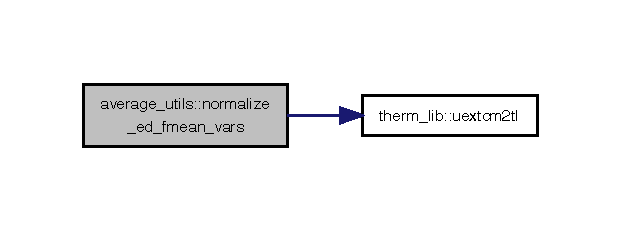
\includegraphics[width=298pt]{namespaceaverage__utils_a662a31926be61beb22be003b5ec40343_cgraph}
\end{center}
\end{figure}
\mbox{\Hypertarget{namespaceaverage__utils_afce18c59b2e9d5605d22e4d356934bdb}\label{namespaceaverage__utils_afce18c59b2e9d5605d22e4d356934bdb}} 
\index{average\+\_\+utils@{average\+\_\+utils}!normalize\+\_\+ed\+\_\+mmean\+\_\+vars@{normalize\+\_\+ed\+\_\+mmean\+\_\+vars}}
\index{normalize\+\_\+ed\+\_\+mmean\+\_\+vars@{normalize\+\_\+ed\+\_\+mmean\+\_\+vars}!average\+\_\+utils@{average\+\_\+utils}}
\subsubsection{\texorpdfstring{normalize\+\_\+ed\+\_\+mmean\+\_\+vars()}{normalize\_ed\_mmean\_vars()}}
{\footnotesize\ttfamily subroutine average\+\_\+utils\+::normalize\+\_\+ed\+\_\+mmean\+\_\+vars (\begin{DoxyParamCaption}\item[{type(edtype), target}]{cgrid }\end{DoxyParamCaption})}

Here is the call graph for this function\+:
\nopagebreak
\begin{figure}[H]
\begin{center}
\leavevmode
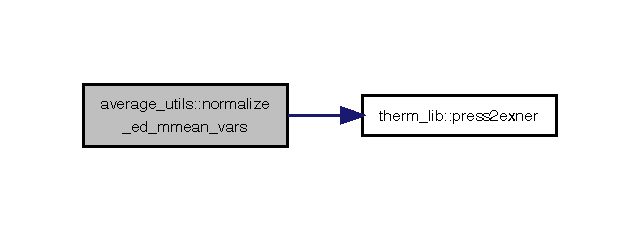
\includegraphics[width=307pt]{namespaceaverage__utils_afce18c59b2e9d5605d22e4d356934bdb_cgraph}
\end{center}
\end{figure}
\mbox{\Hypertarget{namespaceaverage__utils_ad7f232f9a24079c3430b005098729615}\label{namespaceaverage__utils_ad7f232f9a24079c3430b005098729615}} 
\index{average\+\_\+utils@{average\+\_\+utils}!normalize\+\_\+ed\+\_\+qmean\+\_\+vars@{normalize\+\_\+ed\+\_\+qmean\+\_\+vars}}
\index{normalize\+\_\+ed\+\_\+qmean\+\_\+vars@{normalize\+\_\+ed\+\_\+qmean\+\_\+vars}!average\+\_\+utils@{average\+\_\+utils}}
\subsubsection{\texorpdfstring{normalize\+\_\+ed\+\_\+qmean\+\_\+vars()}{normalize\_ed\_qmean\_vars()}}
{\footnotesize\ttfamily subroutine average\+\_\+utils\+::normalize\+\_\+ed\+\_\+qmean\+\_\+vars (\begin{DoxyParamCaption}\item[{type(edtype), target}]{cgrid }\end{DoxyParamCaption})}

Here is the call graph for this function\+:
\nopagebreak
\begin{figure}[H]
\begin{center}
\leavevmode
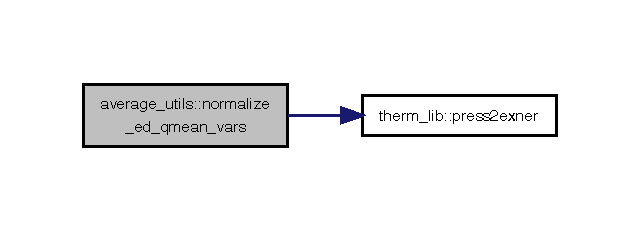
\includegraphics[width=307pt]{namespaceaverage__utils_ad7f232f9a24079c3430b005098729615_cgraph}
\end{center}
\end{figure}
\mbox{\Hypertarget{namespaceaverage__utils_a538e2e59c7c2889ae624b6e1d2a9e5f2}\label{namespaceaverage__utils_a538e2e59c7c2889ae624b6e1d2a9e5f2}} 
\index{average\+\_\+utils@{average\+\_\+utils}!normalize\+\_\+ed\+\_\+today\+\_\+vars@{normalize\+\_\+ed\+\_\+today\+\_\+vars}}
\index{normalize\+\_\+ed\+\_\+today\+\_\+vars@{normalize\+\_\+ed\+\_\+today\+\_\+vars}!average\+\_\+utils@{average\+\_\+utils}}
\subsubsection{\texorpdfstring{normalize\+\_\+ed\+\_\+today\+\_\+vars()}{normalize\_ed\_today\_vars()}}
{\footnotesize\ttfamily subroutine average\+\_\+utils\+::normalize\+\_\+ed\+\_\+today\+\_\+vars (\begin{DoxyParamCaption}\item[{type(edtype), target}]{cgrid }\end{DoxyParamCaption})}

Here is the caller graph for this function\+:
\nopagebreak
\begin{figure}[H]
\begin{center}
\leavevmode
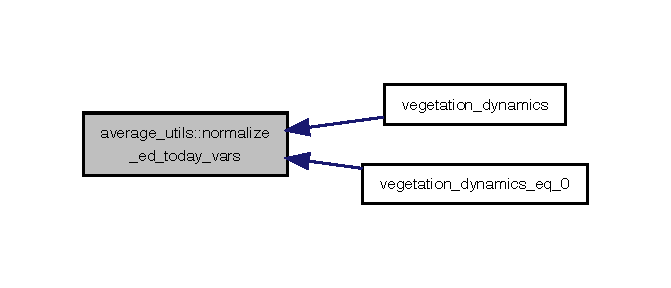
\includegraphics[width=322pt]{namespaceaverage__utils_a538e2e59c7c2889ae624b6e1d2a9e5f2_icgraph}
\end{center}
\end{figure}
\mbox{\Hypertarget{namespaceaverage__utils_a446f9090fbbcf3eb12f4b9231d946e89}\label{namespaceaverage__utils_a446f9090fbbcf3eb12f4b9231d946e89}} 
\index{average\+\_\+utils@{average\+\_\+utils}!normalize\+\_\+ed\+\_\+todaynpp\+\_\+vars@{normalize\+\_\+ed\+\_\+todaynpp\+\_\+vars}}
\index{normalize\+\_\+ed\+\_\+todaynpp\+\_\+vars@{normalize\+\_\+ed\+\_\+todaynpp\+\_\+vars}!average\+\_\+utils@{average\+\_\+utils}}
\subsubsection{\texorpdfstring{normalize\+\_\+ed\+\_\+todaynpp\+\_\+vars()}{normalize\_ed\_todaynpp\_vars()}}
{\footnotesize\ttfamily subroutine average\+\_\+utils\+::normalize\+\_\+ed\+\_\+todaynpp\+\_\+vars (\begin{DoxyParamCaption}\item[{type(edtype), target}]{cgrid }\end{DoxyParamCaption})}

\mbox{\Hypertarget{namespaceaverage__utils_a81384775dd05dba144bf83e9731d5275}\label{namespaceaverage__utils_a81384775dd05dba144bf83e9731d5275}} 
\index{average\+\_\+utils@{average\+\_\+utils}!update\+\_\+ed\+\_\+yearly\+\_\+vars@{update\+\_\+ed\+\_\+yearly\+\_\+vars}}
\index{update\+\_\+ed\+\_\+yearly\+\_\+vars@{update\+\_\+ed\+\_\+yearly\+\_\+vars}!average\+\_\+utils@{average\+\_\+utils}}
\subsubsection{\texorpdfstring{update\+\_\+ed\+\_\+yearly\+\_\+vars()}{update\_ed\_yearly\_vars()}}
{\footnotesize\ttfamily subroutine average\+\_\+utils\+::update\+\_\+ed\+\_\+yearly\+\_\+vars (\begin{DoxyParamCaption}\item[{type(edtype), target}]{cgrid }\end{DoxyParamCaption})}

\mbox{\Hypertarget{namespaceaverage__utils_af1a2224da3c590c5645db8efa5c16c9f}\label{namespaceaverage__utils_af1a2224da3c590c5645db8efa5c16c9f}} 
\index{average\+\_\+utils@{average\+\_\+utils}!zero\+\_\+ed\+\_\+dmean\+\_\+vars@{zero\+\_\+ed\+\_\+dmean\+\_\+vars}}
\index{zero\+\_\+ed\+\_\+dmean\+\_\+vars@{zero\+\_\+ed\+\_\+dmean\+\_\+vars}!average\+\_\+utils@{average\+\_\+utils}}
\subsubsection{\texorpdfstring{zero\+\_\+ed\+\_\+dmean\+\_\+vars()}{zero\_ed\_dmean\_vars()}}
{\footnotesize\ttfamily subroutine average\+\_\+utils\+::zero\+\_\+ed\+\_\+dmean\+\_\+vars (\begin{DoxyParamCaption}\item[{type(edtype), target}]{cgrid }\end{DoxyParamCaption})}

\mbox{\Hypertarget{namespaceaverage__utils_a40f7a4a46972fb6b9c0fe90fdc73a173}\label{namespaceaverage__utils_a40f7a4a46972fb6b9c0fe90fdc73a173}} 
\index{average\+\_\+utils@{average\+\_\+utils}!zero\+\_\+ed\+\_\+fmean\+\_\+vars@{zero\+\_\+ed\+\_\+fmean\+\_\+vars}}
\index{zero\+\_\+ed\+\_\+fmean\+\_\+vars@{zero\+\_\+ed\+\_\+fmean\+\_\+vars}!average\+\_\+utils@{average\+\_\+utils}}
\subsubsection{\texorpdfstring{zero\+\_\+ed\+\_\+fmean\+\_\+vars()}{zero\_ed\_fmean\_vars()}}
{\footnotesize\ttfamily subroutine average\+\_\+utils\+::zero\+\_\+ed\+\_\+fmean\+\_\+vars (\begin{DoxyParamCaption}\item[{type(edtype), target}]{cgrid }\end{DoxyParamCaption})}

\mbox{\Hypertarget{namespaceaverage__utils_aa5221fd3b377dfe424dbdcb81b83c378}\label{namespaceaverage__utils_aa5221fd3b377dfe424dbdcb81b83c378}} 
\index{average\+\_\+utils@{average\+\_\+utils}!zero\+\_\+ed\+\_\+mmean\+\_\+vars@{zero\+\_\+ed\+\_\+mmean\+\_\+vars}}
\index{zero\+\_\+ed\+\_\+mmean\+\_\+vars@{zero\+\_\+ed\+\_\+mmean\+\_\+vars}!average\+\_\+utils@{average\+\_\+utils}}
\subsubsection{\texorpdfstring{zero\+\_\+ed\+\_\+mmean\+\_\+vars()}{zero\_ed\_mmean\_vars()}}
{\footnotesize\ttfamily subroutine average\+\_\+utils\+::zero\+\_\+ed\+\_\+mmean\+\_\+vars (\begin{DoxyParamCaption}\item[{type(edtype), target}]{cgrid }\end{DoxyParamCaption})}

\mbox{\Hypertarget{namespaceaverage__utils_a2e9cb2592327099345c147516b927f51}\label{namespaceaverage__utils_a2e9cb2592327099345c147516b927f51}} 
\index{average\+\_\+utils@{average\+\_\+utils}!zero\+\_\+ed\+\_\+qmean\+\_\+vars@{zero\+\_\+ed\+\_\+qmean\+\_\+vars}}
\index{zero\+\_\+ed\+\_\+qmean\+\_\+vars@{zero\+\_\+ed\+\_\+qmean\+\_\+vars}!average\+\_\+utils@{average\+\_\+utils}}
\subsubsection{\texorpdfstring{zero\+\_\+ed\+\_\+qmean\+\_\+vars()}{zero\_ed\_qmean\_vars()}}
{\footnotesize\ttfamily subroutine average\+\_\+utils\+::zero\+\_\+ed\+\_\+qmean\+\_\+vars (\begin{DoxyParamCaption}\item[{type(edtype), target}]{cgrid }\end{DoxyParamCaption})}

\mbox{\Hypertarget{namespaceaverage__utils_a6a92d00bf7112b127a596bd765cc12c6}\label{namespaceaverage__utils_a6a92d00bf7112b127a596bd765cc12c6}} 
\index{average\+\_\+utils@{average\+\_\+utils}!zero\+\_\+ed\+\_\+today\+\_\+vars@{zero\+\_\+ed\+\_\+today\+\_\+vars}}
\index{zero\+\_\+ed\+\_\+today\+\_\+vars@{zero\+\_\+ed\+\_\+today\+\_\+vars}!average\+\_\+utils@{average\+\_\+utils}}
\subsubsection{\texorpdfstring{zero\+\_\+ed\+\_\+today\+\_\+vars()}{zero\_ed\_today\_vars()}}
{\footnotesize\ttfamily subroutine average\+\_\+utils\+::zero\+\_\+ed\+\_\+today\+\_\+vars (\begin{DoxyParamCaption}\item[{type(edtype), target}]{cgrid }\end{DoxyParamCaption})}

\mbox{\Hypertarget{namespaceaverage__utils_a81df7cc84b1d62f7fb950e91d410abbd}\label{namespaceaverage__utils_a81df7cc84b1d62f7fb950e91d410abbd}} 
\index{average\+\_\+utils@{average\+\_\+utils}!zero\+\_\+ed\+\_\+yearly\+\_\+vars@{zero\+\_\+ed\+\_\+yearly\+\_\+vars}}
\index{zero\+\_\+ed\+\_\+yearly\+\_\+vars@{zero\+\_\+ed\+\_\+yearly\+\_\+vars}!average\+\_\+utils@{average\+\_\+utils}}
\subsubsection{\texorpdfstring{zero\+\_\+ed\+\_\+yearly\+\_\+vars()}{zero\_ed\_yearly\_vars()}}
{\footnotesize\ttfamily subroutine average\+\_\+utils\+::zero\+\_\+ed\+\_\+yearly\+\_\+vars (\begin{DoxyParamCaption}\item[{type(edtype), target}]{cgrid }\end{DoxyParamCaption})}


\hypertarget{namespacebudget__utils}{}\section{budget\+\_\+utils Module Reference}
\label{namespacebudget__utils}\index{budget\+\_\+utils@{budget\+\_\+utils}}
\subsection*{Functions/\+Subroutines}
\begin{DoxyCompactItemize}
\item 
subroutine \hyperlink{namespacebudget__utils_ac092645bc3b3bd0dcfa2cdedc2451c58}{update\+\_\+budget} (csite, lsl, ipa)
\item 
subroutine \hyperlink{namespacebudget__utils_a07d8e19ed53707603c43556eb24b5fea}{compute\+\_\+budget} (csite, lsl, pcpg, qpcpg, ipa, wcurr\+\_\+loss2atm, ecurr\+\_\+netrad, ecurr\+\_\+loss2atm, co2curr\+\_\+loss2atm, wcurr\+\_\+loss2drainage, ecurr\+\_\+loss2drainage, wcurr\+\_\+loss2runoff, ecurr\+\_\+loss2runoff, site\+\_\+area, cbudget\+\_\+nep, old\+\_\+can\+\_\+enthalpy, old\+\_\+can\+\_\+shv, old\+\_\+can\+\_\+co2, old\+\_\+can\+\_\+rhos, old\+\_\+can\+\_\+prss)
\item 
real function \hyperlink{namespacebudget__utils_ad0c764047c557100b3a3cdcd836103a0}{compute\+\_\+water\+\_\+storage} (csite, lsl, ipa)
\item 
real function \hyperlink{namespacebudget__utils_a6111a1c211ecef562368c8635f64af45}{compute\+\_\+netrad} (csite, ipa)
\item 
real function \hyperlink{namespacebudget__utils_a319c5f7252c344bcebbd162593e25ec8}{compute\+\_\+energy\+\_\+storage} (csite, lsl, ipa)
\item 
subroutine \hyperlink{namespacebudget__utils_ae3ca69dd43d1f92a0a86e21fcd57c641}{sum\+\_\+plant\+\_\+cfluxes} (csite, ipa, gpp, leaf\+\_\+resp, root\+\_\+resp, leaf\+\_\+growth\+\_\+resp, root\+\_\+growth\+\_\+resp, sapa\+\_\+growth\+\_\+resp, sapb\+\_\+growth\+\_\+resp, leaf\+\_\+storage\+\_\+resp, root\+\_\+storage\+\_\+resp, sapa\+\_\+storage\+\_\+resp, sapb\+\_\+storage\+\_\+resp)
\item 
real function \hyperlink{namespacebudget__utils_aa1c4f8466010b1673f2914f1bfe9b6ee}{compute\+\_\+co2\+\_\+storage} (csite, ipa)
\item 
real function \hyperlink{namespacebudget__utils_ae7ad8d90c28490b0b1c920e7a2656345}{ddens\+\_\+dt\+\_\+effect} (old\+\_\+rhos, new\+\_\+rhos, old\+\_\+prop, new\+\_\+prop, can\+\_\+depth, multi)
\end{DoxyCompactItemize}


\subsection{Function/\+Subroutine Documentation}
\mbox{\Hypertarget{namespacebudget__utils_a07d8e19ed53707603c43556eb24b5fea}\label{namespacebudget__utils_a07d8e19ed53707603c43556eb24b5fea}} 
\index{budget\+\_\+utils@{budget\+\_\+utils}!compute\+\_\+budget@{compute\+\_\+budget}}
\index{compute\+\_\+budget@{compute\+\_\+budget}!budget\+\_\+utils@{budget\+\_\+utils}}
\subsubsection{\texorpdfstring{compute\+\_\+budget()}{compute\_budget()}}
{\footnotesize\ttfamily subroutine budget\+\_\+utils\+::compute\+\_\+budget (\begin{DoxyParamCaption}\item[{type(sitetype), target}]{csite,  }\item[{integer, intent(in)}]{lsl,  }\item[{real, intent(inout)}]{pcpg,  }\item[{real, intent(inout)}]{qpcpg,  }\item[{integer, intent(in)}]{ipa,  }\item[{real, intent(inout)}]{wcurr\+\_\+loss2atm,  }\item[{real, intent(inout)}]{ecurr\+\_\+netrad,  }\item[{real, intent(inout)}]{ecurr\+\_\+loss2atm,  }\item[{real, intent(inout)}]{co2curr\+\_\+loss2atm,  }\item[{real, intent(inout)}]{wcurr\+\_\+loss2drainage,  }\item[{real, intent(inout)}]{ecurr\+\_\+loss2drainage,  }\item[{real, intent(inout)}]{wcurr\+\_\+loss2runoff,  }\item[{real, intent(inout)}]{ecurr\+\_\+loss2runoff,  }\item[{real, intent(in)}]{site\+\_\+area,  }\item[{real, intent(inout)}]{cbudget\+\_\+nep,  }\item[{real, intent(in)}]{old\+\_\+can\+\_\+enthalpy,  }\item[{real, intent(in)}]{old\+\_\+can\+\_\+shv,  }\item[{real, intent(in)}]{old\+\_\+can\+\_\+co2,  }\item[{real, intent(in)}]{old\+\_\+can\+\_\+rhos,  }\item[{real, intent(in)}]{old\+\_\+can\+\_\+prss }\end{DoxyParamCaption})}

Here is the call graph for this function\+:
\nopagebreak
\begin{figure}[H]
\begin{center}
\leavevmode
\includegraphics[width=350pt]{namespacebudget__utils_a07d8e19ed53707603c43556eb24b5fea_cgraph}
\end{center}
\end{figure}
\mbox{\Hypertarget{namespacebudget__utils_aa1c4f8466010b1673f2914f1bfe9b6ee}\label{namespacebudget__utils_aa1c4f8466010b1673f2914f1bfe9b6ee}} 
\index{budget\+\_\+utils@{budget\+\_\+utils}!compute\+\_\+co2\+\_\+storage@{compute\+\_\+co2\+\_\+storage}}
\index{compute\+\_\+co2\+\_\+storage@{compute\+\_\+co2\+\_\+storage}!budget\+\_\+utils@{budget\+\_\+utils}}
\subsubsection{\texorpdfstring{compute\+\_\+co2\+\_\+storage()}{compute\_co2\_storage()}}
{\footnotesize\ttfamily real function budget\+\_\+utils\+::compute\+\_\+co2\+\_\+storage (\begin{DoxyParamCaption}\item[{type(sitetype), target}]{csite,  }\item[{integer, intent(in)}]{ipa }\end{DoxyParamCaption})}

Here is the caller graph for this function\+:
\nopagebreak
\begin{figure}[H]
\begin{center}
\leavevmode
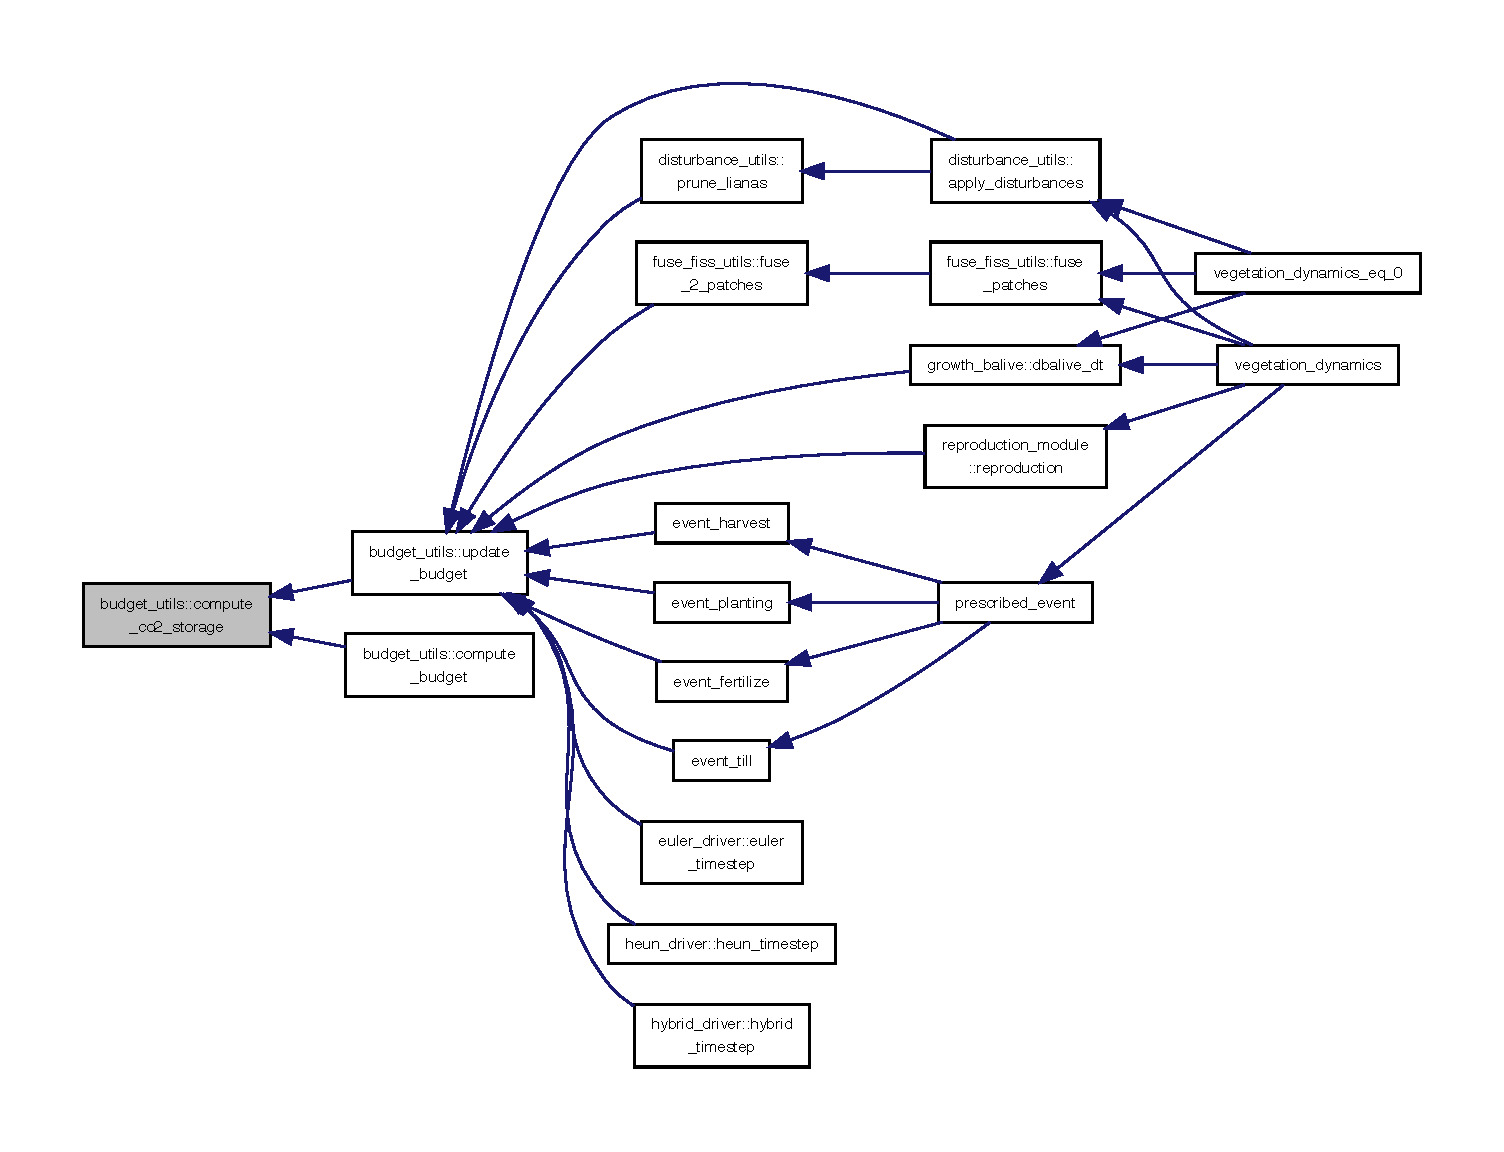
\includegraphics[width=350pt]{namespacebudget__utils_aa1c4f8466010b1673f2914f1bfe9b6ee_icgraph}
\end{center}
\end{figure}
\mbox{\Hypertarget{namespacebudget__utils_a319c5f7252c344bcebbd162593e25ec8}\label{namespacebudget__utils_a319c5f7252c344bcebbd162593e25ec8}} 
\index{budget\+\_\+utils@{budget\+\_\+utils}!compute\+\_\+energy\+\_\+storage@{compute\+\_\+energy\+\_\+storage}}
\index{compute\+\_\+energy\+\_\+storage@{compute\+\_\+energy\+\_\+storage}!budget\+\_\+utils@{budget\+\_\+utils}}
\subsubsection{\texorpdfstring{compute\+\_\+energy\+\_\+storage()}{compute\_energy\_storage()}}
{\footnotesize\ttfamily real function budget\+\_\+utils\+::compute\+\_\+energy\+\_\+storage (\begin{DoxyParamCaption}\item[{type(sitetype), target}]{csite,  }\item[{integer, intent(in)}]{lsl,  }\item[{integer, intent(in)}]{ipa }\end{DoxyParamCaption})}

Here is the call graph for this function\+:
\nopagebreak
\begin{figure}[H]
\begin{center}
\leavevmode
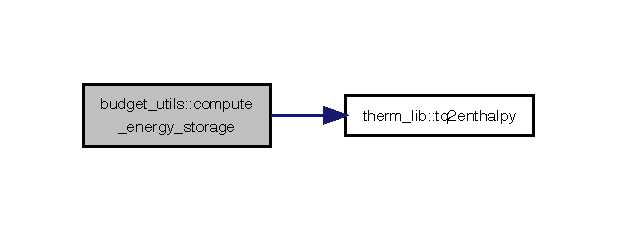
\includegraphics[width=296pt]{namespacebudget__utils_a319c5f7252c344bcebbd162593e25ec8_cgraph}
\end{center}
\end{figure}
Here is the caller graph for this function\+:
\nopagebreak
\begin{figure}[H]
\begin{center}
\leavevmode
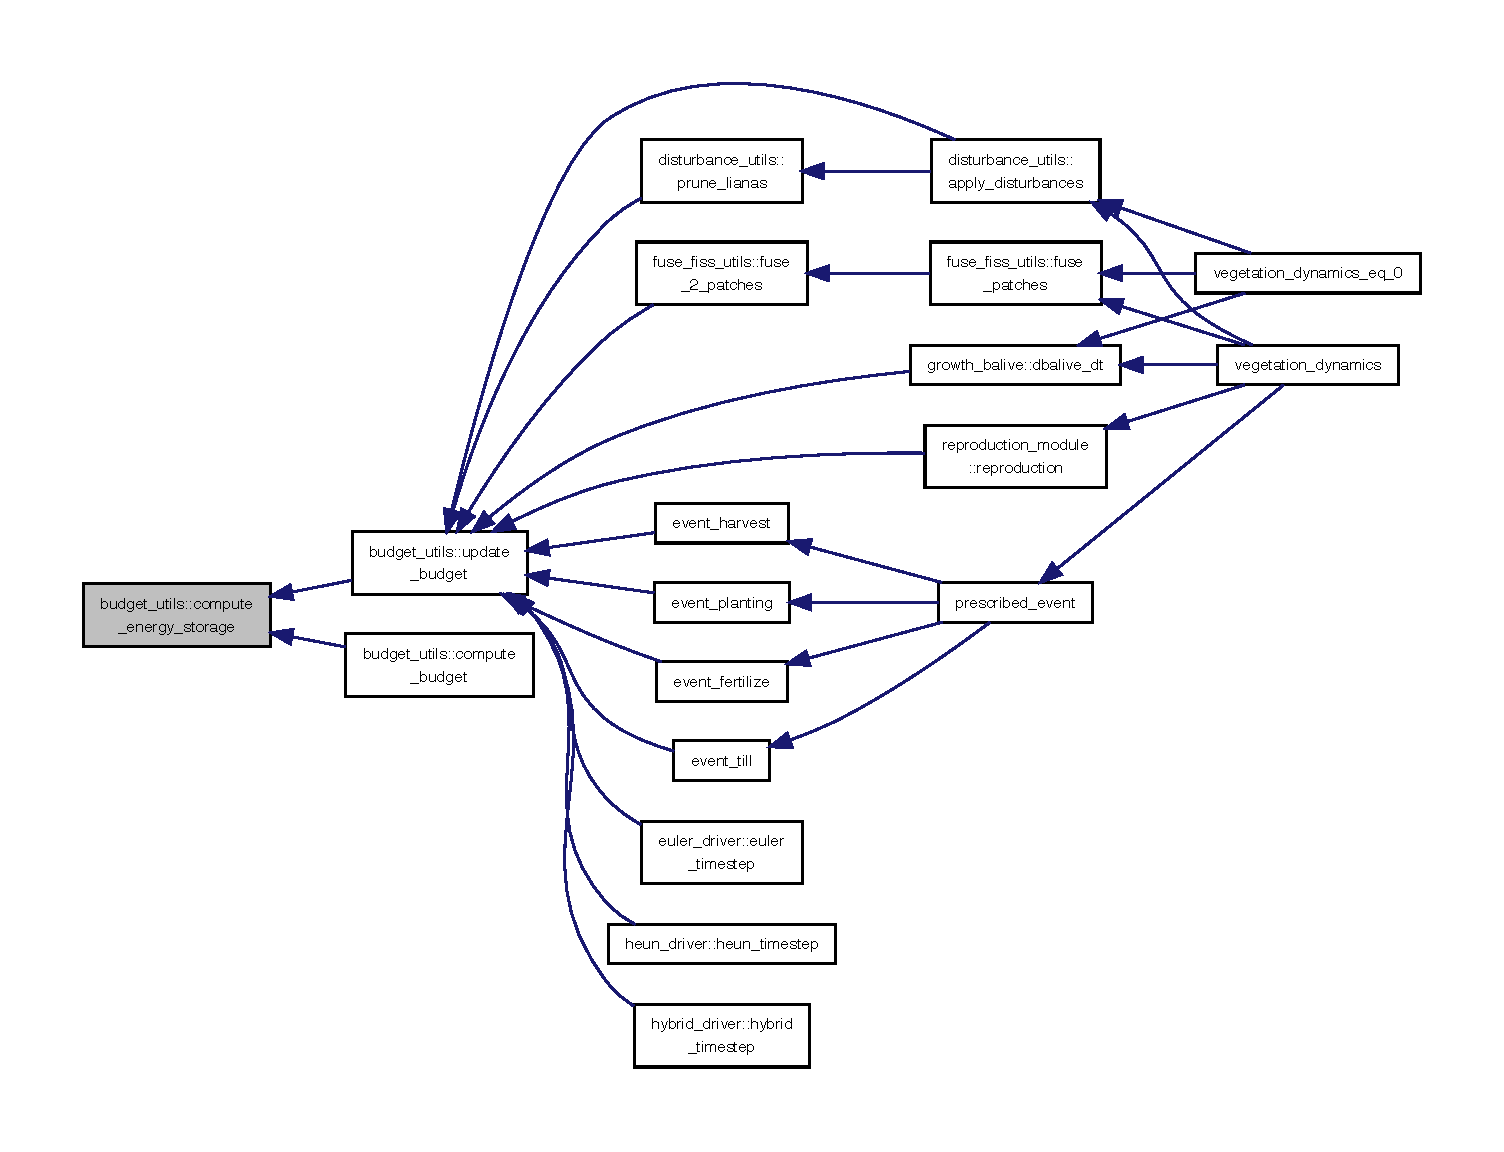
\includegraphics[width=350pt]{namespacebudget__utils_a319c5f7252c344bcebbd162593e25ec8_icgraph}
\end{center}
\end{figure}
\mbox{\Hypertarget{namespacebudget__utils_a6111a1c211ecef562368c8635f64af45}\label{namespacebudget__utils_a6111a1c211ecef562368c8635f64af45}} 
\index{budget\+\_\+utils@{budget\+\_\+utils}!compute\+\_\+netrad@{compute\+\_\+netrad}}
\index{compute\+\_\+netrad@{compute\+\_\+netrad}!budget\+\_\+utils@{budget\+\_\+utils}}
\subsubsection{\texorpdfstring{compute\+\_\+netrad()}{compute\_netrad()}}
{\footnotesize\ttfamily real function budget\+\_\+utils\+::compute\+\_\+netrad (\begin{DoxyParamCaption}\item[{type(sitetype), target}]{csite,  }\item[{integer, intent(in)}]{ipa }\end{DoxyParamCaption})}

\mbox{\Hypertarget{namespacebudget__utils_ad0c764047c557100b3a3cdcd836103a0}\label{namespacebudget__utils_ad0c764047c557100b3a3cdcd836103a0}} 
\index{budget\+\_\+utils@{budget\+\_\+utils}!compute\+\_\+water\+\_\+storage@{compute\+\_\+water\+\_\+storage}}
\index{compute\+\_\+water\+\_\+storage@{compute\+\_\+water\+\_\+storage}!budget\+\_\+utils@{budget\+\_\+utils}}
\subsubsection{\texorpdfstring{compute\+\_\+water\+\_\+storage()}{compute\_water\_storage()}}
{\footnotesize\ttfamily real function budget\+\_\+utils\+::compute\+\_\+water\+\_\+storage (\begin{DoxyParamCaption}\item[{type(sitetype), target}]{csite,  }\item[{integer, intent(in)}]{lsl,  }\item[{integer, intent(in)}]{ipa }\end{DoxyParamCaption})}

Here is the caller graph for this function\+:
\nopagebreak
\begin{figure}[H]
\begin{center}
\leavevmode
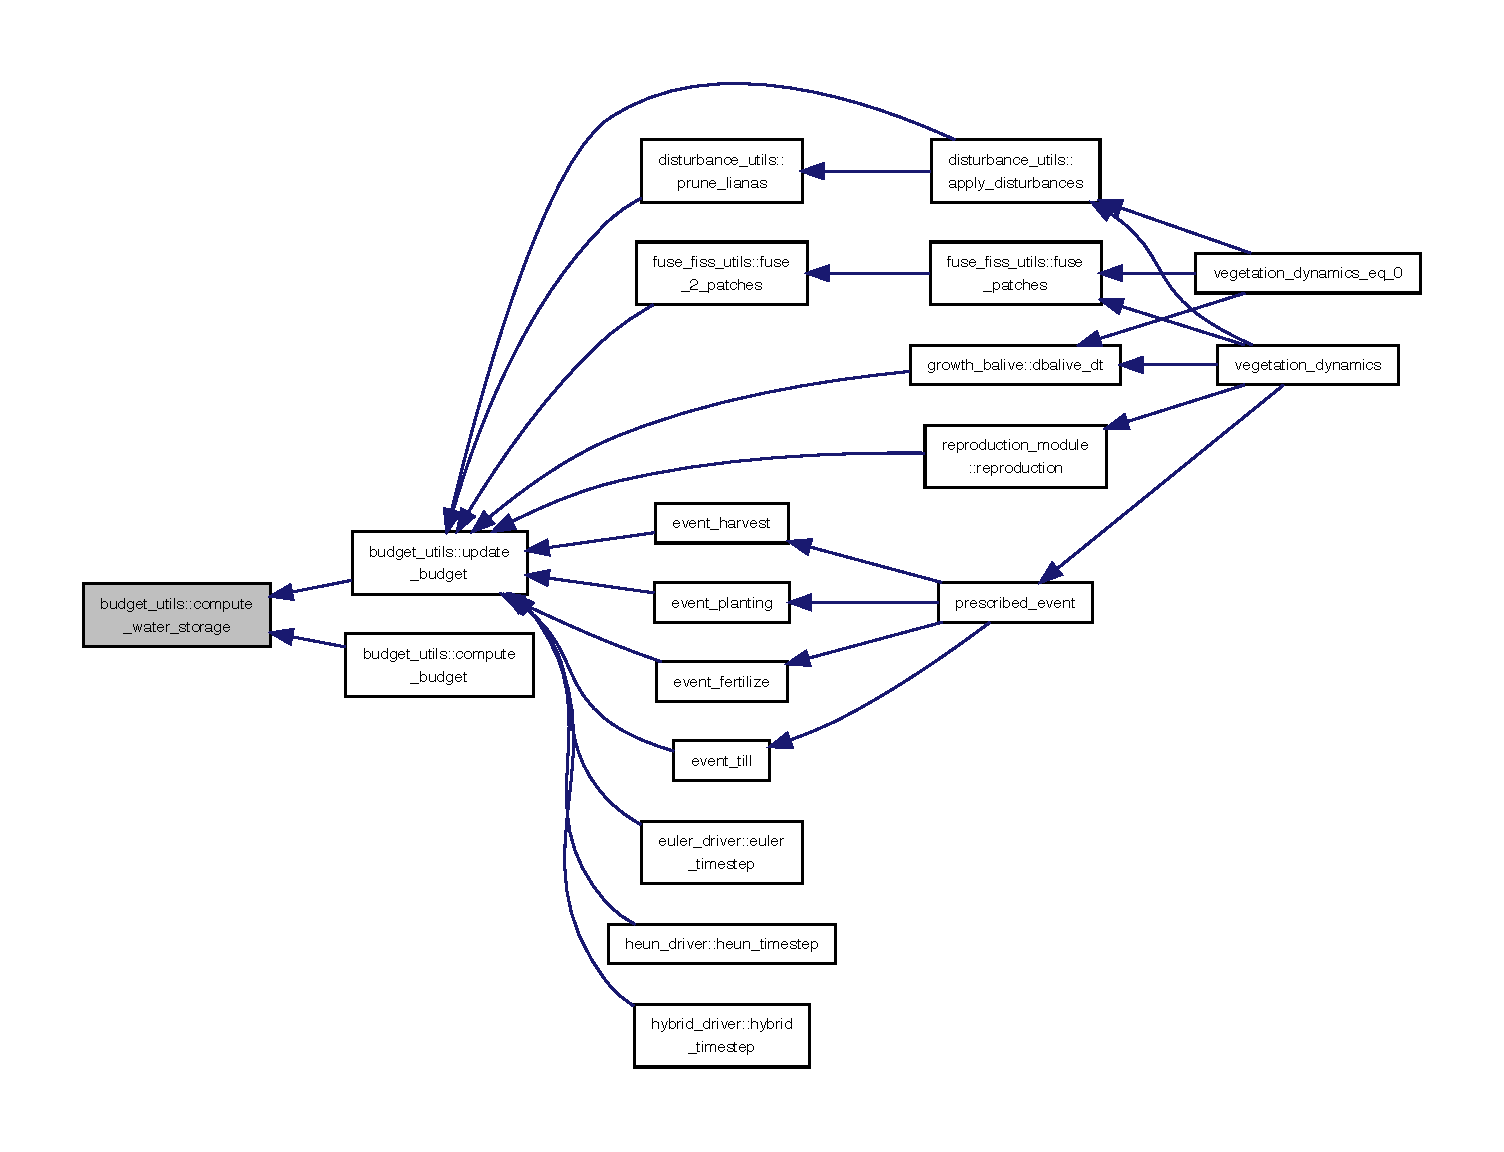
\includegraphics[width=350pt]{namespacebudget__utils_ad0c764047c557100b3a3cdcd836103a0_icgraph}
\end{center}
\end{figure}
\mbox{\Hypertarget{namespacebudget__utils_ae7ad8d90c28490b0b1c920e7a2656345}\label{namespacebudget__utils_ae7ad8d90c28490b0b1c920e7a2656345}} 
\index{budget\+\_\+utils@{budget\+\_\+utils}!ddens\+\_\+dt\+\_\+effect@{ddens\+\_\+dt\+\_\+effect}}
\index{ddens\+\_\+dt\+\_\+effect@{ddens\+\_\+dt\+\_\+effect}!budget\+\_\+utils@{budget\+\_\+utils}}
\subsubsection{\texorpdfstring{ddens\+\_\+dt\+\_\+effect()}{ddens\_dt\_effect()}}
{\footnotesize\ttfamily real function budget\+\_\+utils\+::ddens\+\_\+dt\+\_\+effect (\begin{DoxyParamCaption}\item[{real, intent(in)}]{old\+\_\+rhos,  }\item[{real, intent(in)}]{new\+\_\+rhos,  }\item[{real, intent(in)}]{old\+\_\+prop,  }\item[{real, intent(in)}]{new\+\_\+prop,  }\item[{real, intent(in)}]{can\+\_\+depth,  }\item[{real, intent(in)}]{multi }\end{DoxyParamCaption})}

Here is the caller graph for this function\+:
\nopagebreak
\begin{figure}[H]
\begin{center}
\leavevmode
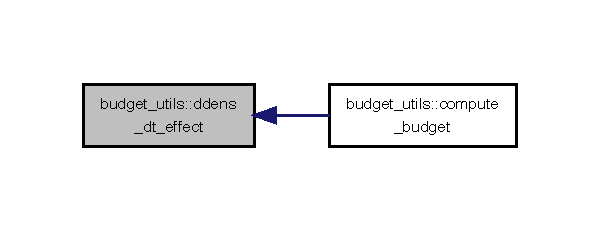
\includegraphics[width=288pt]{namespacebudget__utils_ae7ad8d90c28490b0b1c920e7a2656345_icgraph}
\end{center}
\end{figure}
\mbox{\Hypertarget{namespacebudget__utils_ae3ca69dd43d1f92a0a86e21fcd57c641}\label{namespacebudget__utils_ae3ca69dd43d1f92a0a86e21fcd57c641}} 
\index{budget\+\_\+utils@{budget\+\_\+utils}!sum\+\_\+plant\+\_\+cfluxes@{sum\+\_\+plant\+\_\+cfluxes}}
\index{sum\+\_\+plant\+\_\+cfluxes@{sum\+\_\+plant\+\_\+cfluxes}!budget\+\_\+utils@{budget\+\_\+utils}}
\subsubsection{\texorpdfstring{sum\+\_\+plant\+\_\+cfluxes()}{sum\_plant\_cfluxes()}}
{\footnotesize\ttfamily subroutine budget\+\_\+utils\+::sum\+\_\+plant\+\_\+cfluxes (\begin{DoxyParamCaption}\item[{type(sitetype), target}]{csite,  }\item[{integer, intent(in)}]{ipa,  }\item[{real, intent(out)}]{gpp,  }\item[{real, intent(out)}]{leaf\+\_\+resp,  }\item[{real, intent(out)}]{root\+\_\+resp,  }\item[{real, intent(out)}]{leaf\+\_\+growth\+\_\+resp,  }\item[{real, intent(out)}]{root\+\_\+growth\+\_\+resp,  }\item[{real, intent(out)}]{sapa\+\_\+growth\+\_\+resp,  }\item[{real, intent(out)}]{sapb\+\_\+growth\+\_\+resp,  }\item[{real, intent(out)}]{leaf\+\_\+storage\+\_\+resp,  }\item[{real, intent(out)}]{root\+\_\+storage\+\_\+resp,  }\item[{real, intent(out)}]{sapa\+\_\+storage\+\_\+resp,  }\item[{real, intent(out)}]{sapb\+\_\+storage\+\_\+resp }\end{DoxyParamCaption})}

Here is the caller graph for this function\+:
\nopagebreak
\begin{figure}[H]
\begin{center}
\leavevmode
\includegraphics[width=302pt]{namespacebudget__utils_ae3ca69dd43d1f92a0a86e21fcd57c641_icgraph}
\end{center}
\end{figure}
\mbox{\Hypertarget{namespacebudget__utils_ac092645bc3b3bd0dcfa2cdedc2451c58}\label{namespacebudget__utils_ac092645bc3b3bd0dcfa2cdedc2451c58}} 
\index{budget\+\_\+utils@{budget\+\_\+utils}!update\+\_\+budget@{update\+\_\+budget}}
\index{update\+\_\+budget@{update\+\_\+budget}!budget\+\_\+utils@{budget\+\_\+utils}}
\subsubsection{\texorpdfstring{update\+\_\+budget()}{update\_budget()}}
{\footnotesize\ttfamily subroutine budget\+\_\+utils\+::update\+\_\+budget (\begin{DoxyParamCaption}\item[{type(sitetype), target}]{csite,  }\item[{integer, intent(in)}]{lsl,  }\item[{integer, intent(in)}]{ipa }\end{DoxyParamCaption})}

Here is the call graph for this function\+:
\nopagebreak
\begin{figure}[H]
\begin{center}
\leavevmode
\includegraphics[width=350pt]{namespacebudget__utils_ac092645bc3b3bd0dcfa2cdedc2451c58_cgraph}
\end{center}
\end{figure}
Here is the caller graph for this function\+:
\nopagebreak
\begin{figure}[H]
\begin{center}
\leavevmode
\includegraphics[width=350pt]{namespacebudget__utils_ac092645bc3b3bd0dcfa2cdedc2451c58_icgraph}
\end{center}
\end{figure}

\hypertarget{namespacec34constants}{}\section{c34constants Module Reference}
\label{namespacec34constants}\index{c34constants@{c34constants}}
\subsection*{Data Types}
\begin{DoxyCompactItemize}
\item 
type \hyperlink{structc34constants_1_1carb__demand__vars}{carb\+\_\+demand\+\_\+vars}
\item 
type \hyperlink{structc34constants_1_1farq__consts}{farq\+\_\+consts}
\item 
type \hyperlink{structc34constants_1_1metinp__vars}{metinp\+\_\+vars}
\item 
type \hyperlink{structc34constants_1_1solution__vars}{solution\+\_\+vars}
\end{DoxyCompactItemize}
\subsection*{Functions/\+Subroutines}
\begin{DoxyCompactItemize}
\item 
subroutine \hyperlink{namespacec34constants_a2bf287654403f231d7936113aaeb9cf6}{copy\+\_\+solution} (source\+\_\+sol, target\+\_\+sol)
\end{DoxyCompactItemize}
\subsection*{Variables}
\begin{DoxyCompactItemize}
\item 
type(\hyperlink{structc34constants_1_1farq__consts}{farq\+\_\+consts}), dimension(\+:), pointer \hyperlink{namespacec34constants_a4a1314df0becf145f8a2365aa27d992d}{thispft}
\item 
type(\hyperlink{structc34constants_1_1metinp__vars}{metinp\+\_\+vars}), dimension(\+:), pointer \hyperlink{namespacec34constants_a6d1c98b7c360f24d485be8fc38bdd284}{met}
\item 
type(\hyperlink{structc34constants_1_1carb__demand__vars}{carb\+\_\+demand\+\_\+vars}), dimension(\+:), pointer \hyperlink{namespacec34constants_a844bf4288f019d9dcee7612f54d1e50c}{aparms}
\item 
type(\hyperlink{structc34constants_1_1solution__vars}{solution\+\_\+vars}), dimension(\+:), pointer \hyperlink{namespacec34constants_a5affd928720d3a40f01f1198b68b7fb3}{stopen}
\item 
type(\hyperlink{structc34constants_1_1solution__vars}{solution\+\_\+vars}), dimension(\+:), pointer \hyperlink{namespacec34constants_a083891d928147a7252ada72b49b240a3}{stclosed}
\item 
type(\hyperlink{structc34constants_1_1solution__vars}{solution\+\_\+vars}), dimension(\+:), pointer \hyperlink{namespacec34constants_a54cb2e4894b639d22e50b457b4208cfc}{rubiscolim}
\item 
type(\hyperlink{structc34constants_1_1solution__vars}{solution\+\_\+vars}), dimension(\+:), pointer \hyperlink{namespacec34constants_abed7f7ff7745473ac53005a45206f506}{co2lim}
\item 
type(\hyperlink{structc34constants_1_1solution__vars}{solution\+\_\+vars}), dimension(\+:), pointer \hyperlink{namespacec34constants_af66eea644957075da5a5285e735e143b}{lightlim}
\end{DoxyCompactItemize}


\subsection{Function/\+Subroutine Documentation}
\mbox{\Hypertarget{namespacec34constants_a2bf287654403f231d7936113aaeb9cf6}\label{namespacec34constants_a2bf287654403f231d7936113aaeb9cf6}} 
\index{c34constants@{c34constants}!copy\+\_\+solution@{copy\+\_\+solution}}
\index{copy\+\_\+solution@{copy\+\_\+solution}!c34constants@{c34constants}}
\subsubsection{\texorpdfstring{copy\+\_\+solution()}{copy\_solution()}}
{\footnotesize\ttfamily subroutine c34constants\+::copy\+\_\+solution (\begin{DoxyParamCaption}\item[{type(\hyperlink{structc34constants_1_1solution__vars}{solution\+\_\+vars}), intent(in)}]{source\+\_\+sol,  }\item[{type(\hyperlink{structc34constants_1_1solution__vars}{solution\+\_\+vars}), intent(out)}]{target\+\_\+sol }\end{DoxyParamCaption})}



\subsection{Variable Documentation}
\mbox{\Hypertarget{namespacec34constants_a844bf4288f019d9dcee7612f54d1e50c}\label{namespacec34constants_a844bf4288f019d9dcee7612f54d1e50c}} 
\index{c34constants@{c34constants}!aparms@{aparms}}
\index{aparms@{aparms}!c34constants@{c34constants}}
\subsubsection{\texorpdfstring{aparms}{aparms}}
{\footnotesize\ttfamily type(\hyperlink{structc34constants_1_1carb__demand__vars}{carb\+\_\+demand\+\_\+vars}), dimension(\+:), pointer c34constants\+::aparms}

\mbox{\Hypertarget{namespacec34constants_abed7f7ff7745473ac53005a45206f506}\label{namespacec34constants_abed7f7ff7745473ac53005a45206f506}} 
\index{c34constants@{c34constants}!co2lim@{co2lim}}
\index{co2lim@{co2lim}!c34constants@{c34constants}}
\subsubsection{\texorpdfstring{co2lim}{co2lim}}
{\footnotesize\ttfamily type(\hyperlink{structc34constants_1_1solution__vars}{solution\+\_\+vars}), dimension(\+:), pointer c34constants\+::co2lim}

\mbox{\Hypertarget{namespacec34constants_af66eea644957075da5a5285e735e143b}\label{namespacec34constants_af66eea644957075da5a5285e735e143b}} 
\index{c34constants@{c34constants}!lightlim@{lightlim}}
\index{lightlim@{lightlim}!c34constants@{c34constants}}
\subsubsection{\texorpdfstring{lightlim}{lightlim}}
{\footnotesize\ttfamily type(\hyperlink{structc34constants_1_1solution__vars}{solution\+\_\+vars}), dimension(\+:), pointer c34constants\+::lightlim}

\mbox{\Hypertarget{namespacec34constants_a6d1c98b7c360f24d485be8fc38bdd284}\label{namespacec34constants_a6d1c98b7c360f24d485be8fc38bdd284}} 
\index{c34constants@{c34constants}!met@{met}}
\index{met@{met}!c34constants@{c34constants}}
\subsubsection{\texorpdfstring{met}{met}}
{\footnotesize\ttfamily type(\hyperlink{structc34constants_1_1metinp__vars}{metinp\+\_\+vars} ), dimension(\+:), pointer c34constants\+::met}

\mbox{\Hypertarget{namespacec34constants_a54cb2e4894b639d22e50b457b4208cfc}\label{namespacec34constants_a54cb2e4894b639d22e50b457b4208cfc}} 
\index{c34constants@{c34constants}!rubiscolim@{rubiscolim}}
\index{rubiscolim@{rubiscolim}!c34constants@{c34constants}}
\subsubsection{\texorpdfstring{rubiscolim}{rubiscolim}}
{\footnotesize\ttfamily type(\hyperlink{structc34constants_1_1solution__vars}{solution\+\_\+vars}), dimension(\+:), pointer c34constants\+::rubiscolim}

\mbox{\Hypertarget{namespacec34constants_a083891d928147a7252ada72b49b240a3}\label{namespacec34constants_a083891d928147a7252ada72b49b240a3}} 
\index{c34constants@{c34constants}!stclosed@{stclosed}}
\index{stclosed@{stclosed}!c34constants@{c34constants}}
\subsubsection{\texorpdfstring{stclosed}{stclosed}}
{\footnotesize\ttfamily type(\hyperlink{structc34constants_1_1solution__vars}{solution\+\_\+vars}), dimension(\+:), pointer c34constants\+::stclosed}

\mbox{\Hypertarget{namespacec34constants_a5affd928720d3a40f01f1198b68b7fb3}\label{namespacec34constants_a5affd928720d3a40f01f1198b68b7fb3}} 
\index{c34constants@{c34constants}!stopen@{stopen}}
\index{stopen@{stopen}!c34constants@{c34constants}}
\subsubsection{\texorpdfstring{stopen}{stopen}}
{\footnotesize\ttfamily type(\hyperlink{structc34constants_1_1solution__vars}{solution\+\_\+vars}), dimension(\+:), pointer c34constants\+::stopen}

\mbox{\Hypertarget{namespacec34constants_a4a1314df0becf145f8a2365aa27d992d}\label{namespacec34constants_a4a1314df0becf145f8a2365aa27d992d}} 
\index{c34constants@{c34constants}!thispft@{thispft}}
\index{thispft@{thispft}!c34constants@{c34constants}}
\subsubsection{\texorpdfstring{thispft}{thispft}}
{\footnotesize\ttfamily type(\hyperlink{structc34constants_1_1farq__consts}{farq\+\_\+consts} ), dimension(\+:), pointer c34constants\+::thispft}


\hypertarget{namespacecanopy__air__coms}{}\section{canopy\+\_\+air\+\_\+coms Module Reference}
\label{namespacecanopy__air__coms}\index{canopy\+\_\+air\+\_\+coms@{canopy\+\_\+air\+\_\+coms}}
\subsection*{Functions/\+Subroutines}
\begin{DoxyCompactItemize}
\item 
real function \hyperlink{namespacecanopy__air__coms_ab103fa081460babbe04c9a5a4699be5f}{psim} (zeta, stable)
\item 
real function \hyperlink{namespacecanopy__air__coms_acedb0f66db4b79009a69e87c5fd3ed71}{psih} (zeta, stable)
\item 
real(kind=8) function \hyperlink{namespacecanopy__air__coms_aba7cbe776dbfa9815870ad3686949041}{psim8} (zeta, stable)
\item 
real(kind=8) function \hyperlink{namespacecanopy__air__coms_aef33f0eeea82151a8edb6dc38c4cc921}{psih8} (zeta, stable)
\item 
real function \hyperlink{namespacecanopy__air__coms_af8bc6f1d6999a4b614461cecb85c9b1b}{dpsimdzeta} (zeta, stable)
\item 
real function \hyperlink{namespacecanopy__air__coms_a64552e0380fcb36366b5eb0f624241a3}{dpsihdzeta} (zeta, stable)
\item 
real(kind=8) function \hyperlink{namespacecanopy__air__coms_a51b006ac118f9549aee23ddb61a1bf19}{dpsimdzeta8} (zeta, stable)
\item 
real(kind=8) function \hyperlink{namespacecanopy__air__coms_aa5f9649efc40a05ddc13e1450f30fad3}{dpsihdzeta8} (zeta, stable)
\item 
real function \hyperlink{namespacecanopy__air__coms_a6062471b3381c283205ea8b27383a5e0}{zoobukhov} (rib, zstar, rough, zoz0m, lnzoz0m, zoz0h, lnzoz0h, stable)
\item 
real(kind=8) function \hyperlink{namespacecanopy__air__coms_afef697305b4b30385c5206f48d9e787c}{zoobukhov8} (rib, zstar, rough, zoz0m, lnzoz0m, zoz0h, lnzoz0h, stable)
\item 
real function \hyperlink{namespacecanopy__air__coms_a5251266695c581c8f4058d98f6c86200}{zoobukhov\+\_\+ustar} (rib, zstar, rough, zoz0h, lnzoz0h, kuoustar, stable)
\item 
real(kind=8) function \hyperlink{namespacecanopy__air__coms_a6ef582f46fded1355973730e6a2289f2}{zoobukhov\+\_\+ustar8} (rib, zstar, rough, zoz0h, lnzoz0h, kuoustar, stable)
\end{DoxyCompactItemize}
\subsection*{Variables}
\begin{DoxyCompactItemize}
\item 
integer \hyperlink{namespacecanopy__air__coms_ad7c5174d5bc6bd090e9afff63a3428b4}{icanturb}
\item 
integer \hyperlink{namespacecanopy__air__coms_a25351371b3a5e30c3cabd058d1153399}{isfclyrm}
\item 
integer \hyperlink{namespacecanopy__air__coms_a1c11559607f1960e926e0e2adebdba1b}{ied\+\_\+grndvap}
\item 
real \hyperlink{namespacecanopy__air__coms_aaaf296c47691fcf3aaab5b8929b37368}{leaf\+\_\+maxwhc}
\item 
real \hyperlink{namespacecanopy__air__coms_ac8fd39daadba6dc58037eaf42f48700e}{ubmin}
\item 
real \hyperlink{namespacecanopy__air__coms_a593e8ef887b3317fb55545892af84c50}{ugbmin}
\item 
real \hyperlink{namespacecanopy__air__coms_a9a2322371ed4847814fa98174c092c12}{ustmin}
\item 
real \hyperlink{namespacecanopy__air__coms_abb236f0b21abecb4efde793fd6a1811d}{gamm}
\item 
real \hyperlink{namespacecanopy__air__coms_aec7b65c44519ebe9058cb6c4aa655e8c}{gamh}
\item 
real \hyperlink{namespacecanopy__air__coms_adafee179c1e8ba89437987bc4be9b781}{tprandtl}
\item 
real \hyperlink{namespacecanopy__air__coms_a2ac951854c77e1df16229f0fee8a70a6}{vh2vr}
\item 
real \hyperlink{namespacecanopy__air__coms_ab7f6f46003b1ddabed2345c0ed33372d}{vh2dh}
\item 
real \hyperlink{namespacecanopy__air__coms_a553bcc51d0af126ebd44094dae4cdeac}{ribmax}
\item 
real \hyperlink{namespacecanopy__air__coms_a7ec65e87cc2c74a4f55e05e67272a5c0}{exar}
\item 
real \hyperlink{namespacecanopy__air__coms_a8aa4d4dbd59143c45ab4c52fb326ecd6}{covr}
\item 
real \hyperlink{namespacecanopy__air__coms_a63a4c7242b97f72a903fa4c1213b37f0}{ez}
\item 
real(kind=8) \hyperlink{namespacecanopy__air__coms_ab6719dfbc2c9e8e2f9eddf3bf6f97237}{exar8}
\item 
real(kind=8) \hyperlink{namespacecanopy__air__coms_a4afb828f3fecdf23a54cd6276f714544}{ustmin8}
\item 
real(kind=8) \hyperlink{namespacecanopy__air__coms_a96ad2cd68341db7649720ebd90eab97f}{ugbmin8}
\item 
real(kind=8) \hyperlink{namespacecanopy__air__coms_a436ed31f3d8eafc708115bca8ee30d03}{ubmin8}
\item 
real(kind=8) \hyperlink{namespacecanopy__air__coms_a7899b1f4a3a40f367c48fbaa9b7f2ccd}{ez8}
\item 
real(kind=8) \hyperlink{namespacecanopy__air__coms_a5425e68f350bd521634e2dec3df419cc}{vh2vr8}
\item 
real(kind=8) \hyperlink{namespacecanopy__air__coms_aee89a61c55f84edfb62d0b236dea93c8}{vh2dh8}
\item 
real(kind=8) \hyperlink{namespacecanopy__air__coms_a867a9672f31a44b6def8fc0bdf4eb440}{rasveg\+\_\+min8}
\item 
real(kind=8) \hyperlink{namespacecanopy__air__coms_a3cb44bad4430d800393ec76b7a22a782}{taumin8}
\item 
real(kind=4) \hyperlink{namespacecanopy__air__coms_a768765793f4c4b91a6ccca6d5263ad04}{cdrag0}
\item 
real(kind=4) \hyperlink{namespacecanopy__air__coms_a7b44abfd8d12fe84db70aab86954129c}{cdrag1}
\item 
real(kind=4) \hyperlink{namespacecanopy__air__coms_a1b94794c69c4e42537d77c51167c842f}{cdrag2}
\item 
real(kind=4) \hyperlink{namespacecanopy__air__coms_abaac76316a5a249db322fc990489d388}{cdrag3}
\item 
real(kind=4) \hyperlink{namespacecanopy__air__coms_a11e1c7b747cfb7033e3bf75fe4cdd0bc}{pm0}
\item 
real(kind=4) \hyperlink{namespacecanopy__air__coms_a1f414808e85114a30c83bdf9bbc35af6}{c1\+\_\+m97}
\item 
real(kind=4) \hyperlink{namespacecanopy__air__coms_a47dcf89394a1ea827c110b9ceb601b79}{c2\+\_\+m97}
\item 
real(kind=4) \hyperlink{namespacecanopy__air__coms_a40fc08a843524cc8b4e05ba8766cb930}{c3\+\_\+m97}
\item 
real(kind=4) \hyperlink{namespacecanopy__air__coms_a54402456387b824df174f09157236866}{kvwake}
\item 
real(kind=4) \hyperlink{namespacecanopy__air__coms_ac16bf823a6fc81f0d671fa06ca5de7e7}{alpha\+\_\+m97}
\item 
real(kind=4) \hyperlink{namespacecanopy__air__coms_aee71b7396b4019638189e8d16f29d5bc}{alpha\+\_\+mw99}
\item 
real(kind=4), dimension(3) \hyperlink{namespacecanopy__air__coms_a80914f4f0e8ab35603807486ea39940e}{gamma\+\_\+mw99}
\item 
real(kind=4), dimension(3) \hyperlink{namespacecanopy__air__coms_aa50afa7c99107797c84ed294a6215584}{nu\+\_\+mw99}
\item 
real(kind=4) \hyperlink{namespacecanopy__air__coms_aaf5736b1a385a45d4fb74b566c63c036}{infunc}
\item 
real(kind=4) \hyperlink{namespacecanopy__air__coms_aa5644ca796e2926f845d04ce805b9d9c}{cs\+\_\+dense0}
\item 
real(kind=4) \hyperlink{namespacecanopy__air__coms_a5488ab681543df43e05f68b3647184ec}{gamma\+\_\+clm4}
\item 
real(kind=8) \hyperlink{namespacecanopy__air__coms_a651fd5632f3589ad9cd58b3f6eaf5bcc}{dz\+\_\+m978}
\item 
real(kind=8) \hyperlink{namespacecanopy__air__coms_af3d9254c2bae93060644975c43abb36c}{cdrag08}
\item 
real(kind=8) \hyperlink{namespacecanopy__air__coms_ac953582df4052a2a3539e145f2407c50}{cdrag18}
\item 
real(kind=8) \hyperlink{namespacecanopy__air__coms_ab8484a0111b4ddc92040d0c269e66f3a}{cdrag28}
\item 
real(kind=8) \hyperlink{namespacecanopy__air__coms_ab2603251a0323d37d22ea19a30371dbb}{cdrag38}
\item 
real(kind=8) \hyperlink{namespacecanopy__air__coms_aa4901dce15fa74bcece60c3ddfaf5a7e}{pm08}
\item 
real(kind=8) \hyperlink{namespacecanopy__air__coms_a767d679f796e74175138a9b4fad052df}{c1\+\_\+m978}
\item 
real(kind=8) \hyperlink{namespacecanopy__air__coms_a20b553578d5e2da23387a3c814f19229}{c2\+\_\+m978}
\item 
real(kind=8) \hyperlink{namespacecanopy__air__coms_a9be4a0dac0272c3475840eede662688d}{c3\+\_\+m978}
\item 
real(kind=8) \hyperlink{namespacecanopy__air__coms_aea31639861943125d6b07627648637cf}{kvwake8}
\item 
real(kind=8) \hyperlink{namespacecanopy__air__coms_aaca98abaf4f4ff986bd24a7e1ceea8a6}{alpha\+\_\+m97\+\_\+8}
\item 
real(kind=8) \hyperlink{namespacecanopy__air__coms_a0c11f06e8905d7442da34f32fd5a1f5d}{alpha\+\_\+mw99\+\_\+8}
\item 
real(kind=8), dimension(3) \hyperlink{namespacecanopy__air__coms_abfa660e21167dc9825089920687f3aae}{gamma\+\_\+mw99\+\_\+8}
\item 
real(kind=8), dimension(3) \hyperlink{namespacecanopy__air__coms_ae39097ce08183e89c3ed7ee9fba45cfb}{nu\+\_\+mw99\+\_\+8}
\item 
real(kind=8) \hyperlink{namespacecanopy__air__coms_a2b6e9200766e533bfa58ae0da840321e}{infunc\+\_\+8}
\item 
real(kind=8) \hyperlink{namespacecanopy__air__coms_a9f485b27a7dceff879db585b90660457}{cs\+\_\+dense08}
\item 
real(kind=8) \hyperlink{namespacecanopy__air__coms_ab14ce7f9e39fec25d950aa20ea6ca28b}{gamma\+\_\+clm48}
\item 
real(kind=4) \hyperlink{namespacecanopy__air__coms_a63aa3cee74a44dfccdad43b566c7149c}{aflat\+\_\+turb}
\item 
real(kind=4) \hyperlink{namespacecanopy__air__coms_a478fe27fc0f34c4b09208d0f99bae8e5}{aflat\+\_\+lami}
\item 
real(kind=4) \hyperlink{namespacecanopy__air__coms_a73459e396f65a6dd6e485d7ec6256a4c}{nflat\+\_\+turb}
\item 
real(kind=4) \hyperlink{namespacecanopy__air__coms_aebe2845272883354df889b85b1bad430}{nflat\+\_\+lami}
\item 
real(kind=4) \hyperlink{namespacecanopy__air__coms_a7af62fb9a2088fae5b7f939ead3b0d0f}{bflat\+\_\+turb}
\item 
real(kind=4) \hyperlink{namespacecanopy__air__coms_ac93abb13ce6ffe13f90e305450e3ae47}{bflat\+\_\+lami}
\item 
real(kind=4) \hyperlink{namespacecanopy__air__coms_ac97963c22db07629cd6f65bce4201a0b}{mflat\+\_\+turb}
\item 
real(kind=4) \hyperlink{namespacecanopy__air__coms_ae6457ac7f41cb8b0eead67da3f737a2e}{mflat\+\_\+lami}
\item 
real(kind=4) \hyperlink{namespacecanopy__air__coms_ad9c2e83605f784b3a5f68fc55b0d682d}{ocyli\+\_\+turb}
\item 
real(kind=4) \hyperlink{namespacecanopy__air__coms_aefa9b43396983e571ef5c4d1235b3884}{ocyli\+\_\+lami}
\item 
real(kind=4) \hyperlink{namespacecanopy__air__coms_a42c5385303996a52e2fce111d922eaf2}{acyli\+\_\+turb}
\item 
real(kind=4) \hyperlink{namespacecanopy__air__coms_a910e0e75420e6cd46075062c7da2b565}{acyli\+\_\+lami}
\item 
real(kind=4) \hyperlink{namespacecanopy__air__coms_a683ef393f66f3515c40cd7a3278eaff8}{ncyli\+\_\+turb}
\item 
real(kind=4) \hyperlink{namespacecanopy__air__coms_a4e37d8368e61b099d262a431a74acd3e}{ncyli\+\_\+lami}
\item 
real(kind=4) \hyperlink{namespacecanopy__air__coms_a3a47f10726cc2b08ff03868bcbbd4445}{bcyli\+\_\+turb}
\item 
real(kind=4) \hyperlink{namespacecanopy__air__coms_a5569cc0028fc90fc9c90e5148b2b6af3}{bcyli\+\_\+lami}
\item 
real(kind=4) \hyperlink{namespacecanopy__air__coms_acb919351d7e124fc10afbf6c0bd1e974}{mcyli\+\_\+turb}
\item 
real(kind=4) \hyperlink{namespacecanopy__air__coms_a9cef6c431c5209b9adb077d5cf7f3184}{mcyli\+\_\+lami}
\item 
real(kind=8) \hyperlink{namespacecanopy__air__coms_a74069fab7440b8c4adf33de11779b980}{aflat\+\_\+turb8}
\item 
real(kind=8) \hyperlink{namespacecanopy__air__coms_af642ae1aafe80d1c6e7fde278a2236df}{aflat\+\_\+lami8}
\item 
real(kind=8) \hyperlink{namespacecanopy__air__coms_afd3231b755fb237410e1c5996483b57e}{nflat\+\_\+turb8}
\item 
real(kind=8) \hyperlink{namespacecanopy__air__coms_af9e1b7d0da6156fb9ca9fc9ae5c8eadc}{nflat\+\_\+lami8}
\item 
real(kind=8) \hyperlink{namespacecanopy__air__coms_acb451ffb0cf75be9e6269398d5404f07}{bflat\+\_\+turb8}
\item 
real(kind=8) \hyperlink{namespacecanopy__air__coms_a81f50c2e4f31633b624d8c3682751b7f}{bflat\+\_\+lami8}
\item 
real(kind=8) \hyperlink{namespacecanopy__air__coms_a68b2e1b18a4e08daa7ddf8aa42b9958d}{mflat\+\_\+turb8}
\item 
real(kind=8) \hyperlink{namespacecanopy__air__coms_a5deb3fac84d48b1bc1dcb105eb01722d}{mflat\+\_\+lami8}
\item 
real(kind=8) \hyperlink{namespacecanopy__air__coms_ace22bf19aec35f5683446ad8de930257}{ocyli\+\_\+turb8}
\item 
real(kind=8) \hyperlink{namespacecanopy__air__coms_a6fe72df71f0ed3c59b06b99e7291d5f5}{ocyli\+\_\+lami8}
\item 
real(kind=8) \hyperlink{namespacecanopy__air__coms_a933920d4f406fd57c33f8cef1ca8bb83}{acyli\+\_\+turb8}
\item 
real(kind=8) \hyperlink{namespacecanopy__air__coms_a325f601d72eb729cc4301008156be76b}{acyli\+\_\+lami8}
\item 
real(kind=8) \hyperlink{namespacecanopy__air__coms_ad86960a7895c92e10af6d10cae324f82}{ncyli\+\_\+turb8}
\item 
real(kind=8) \hyperlink{namespacecanopy__air__coms_a6f097ca1a4dda12b169f6686939871c0}{ncyli\+\_\+lami8}
\item 
real(kind=8) \hyperlink{namespacecanopy__air__coms_a2f1fda0ccc380bdd8526ea6e1fecb924}{bcyli\+\_\+turb8}
\item 
real(kind=8) \hyperlink{namespacecanopy__air__coms_ad7c65a1b664eb04c6665e7d5a9fc5380}{bcyli\+\_\+lami8}
\item 
real(kind=8) \hyperlink{namespacecanopy__air__coms_ad1cdd46134a9b31835e735884f28e3d0}{mcyli\+\_\+turb8}
\item 
real(kind=8) \hyperlink{namespacecanopy__air__coms_a2c460170035d9a0e3fd4458a165411f2}{mcyli\+\_\+lami8}
\item 
real(kind=8) \hyperlink{namespacecanopy__air__coms_a9493ec4099bf6cd11334e808cd169e72}{beta\+\_\+lami8}
\item 
real(kind=8) \hyperlink{namespacecanopy__air__coms_a42dff1bd5a176d0269c6456ecbd1be1d}{beta\+\_\+turb8}
\item 
real \hyperlink{namespacecanopy__air__coms_ac5812d4be4754c78cd9f1aad023660ba}{bl79}
\item 
real \hyperlink{namespacecanopy__air__coms_a7f257392c2baec6b0f4fe27bd17f809d}{csm}
\item 
real \hyperlink{namespacecanopy__air__coms_aea71c9950d7caa44dcaae548a1d02058}{csh}
\item 
real \hyperlink{namespacecanopy__air__coms_a74b9e27e0f352ab01d8e4aaa567ad2ce}{dl79}
\item 
real \hyperlink{namespacecanopy__air__coms_a1b58671dba4d2fefd5790694e6563f7c}{beta\+\_\+s}
\item 
real \hyperlink{namespacecanopy__air__coms_a8943107817bd72a2ecf2c8ac35516efc}{abh91}
\item 
real \hyperlink{namespacecanopy__air__coms_a19448a094bac99003898bfd3170277e3}{bbh91}
\item 
real \hyperlink{namespacecanopy__air__coms_ae0cae45535d33e82cf2fe8547c1d8dc2}{cbh91}
\item 
real \hyperlink{namespacecanopy__air__coms_a1b28513486b59cf5dc849476f8a8fb8b}{dbh91}
\item 
real \hyperlink{namespacecanopy__air__coms_a3499170cfdc0dbef4966b323d442e71a}{ebh91}
\item 
real \hyperlink{namespacecanopy__air__coms_ac7b57b769f421b5bb07a3ec88e5c6883}{fbh91}
\item 
real \hyperlink{namespacecanopy__air__coms_adc430e44db14a933a4e8359ca834f454}{cod}
\item 
real \hyperlink{namespacecanopy__air__coms_a6a1bee0c06adf9bb369d6f4be822b553}{bcod}
\item 
real \hyperlink{namespacecanopy__air__coms_a41f3ccd2dbb2ccf460109a71a4f66d89}{fm1}
\item 
real \hyperlink{namespacecanopy__air__coms_ae25648cf7af6ad979525a213bc95b1b3}{ate}
\item 
real \hyperlink{namespacecanopy__air__coms_a5fa870deca6638beca69104f25090cc6}{atetf}
\item 
real \hyperlink{namespacecanopy__air__coms_a830ea7ede87dfca30dde16179c04172e}{z0moz0h}
\item 
real \hyperlink{namespacecanopy__air__coms_a8c832d21677dc5ff228d7717066c04b0}{z0hoz0m}
\item 
real \hyperlink{namespacecanopy__air__coms_ad363ff87eeee7cb190ebe28e9b682f9a}{beta\+\_\+vs}
\item 
real \hyperlink{namespacecanopy__air__coms_ac8d65859576c96d4d161e975d040b083}{chim}
\item 
real \hyperlink{namespacecanopy__air__coms_a3afe3afdcc5b2015a51b7072b67354d6}{chih}
\item 
real \hyperlink{namespacecanopy__air__coms_a336486cace202aa0ccad3309337c68f5}{zetac\+\_\+um}
\item 
real \hyperlink{namespacecanopy__air__coms_a22bb3e31261ca100bb41c7413b22c9bf}{zetac\+\_\+uh}
\item 
real \hyperlink{namespacecanopy__air__coms_a72a86a5fffac73ad56991aa0ca9827d4}{zetac\+\_\+sm}
\item 
real \hyperlink{namespacecanopy__air__coms_a11e1cdd8db228dc78ea7ddef9d6414d1}{zetac\+\_\+sh}
\item 
real \hyperlink{namespacecanopy__air__coms_abf9c0a3d2a8c55db802325a22226d5ad}{zetac\+\_\+umi}
\item 
real \hyperlink{namespacecanopy__air__coms_a99110673906c4d2b492c4655450479ba}{zetac\+\_\+uhi}
\item 
real \hyperlink{namespacecanopy__air__coms_ab653a7e7d40e6ec2598a29d6e9a3a50e}{zetac\+\_\+smi}
\item 
real \hyperlink{namespacecanopy__air__coms_a093aae0805de0a745265adb8868298c8}{zetac\+\_\+shi}
\item 
real \hyperlink{namespacecanopy__air__coms_a764636db2f86a1adc1905d691bde4360}{zetac\+\_\+umi16}
\item 
real \hyperlink{namespacecanopy__air__coms_a74f8e50cf094e01598a35c211c67b723}{zetac\+\_\+uhi13}
\item 
real \hyperlink{namespacecanopy__air__coms_abf26fb907b070d554b4addfe5435bc83}{psimc\+\_\+um}
\item 
real \hyperlink{namespacecanopy__air__coms_a09727ee189e0154ebee372935fe46050}{psihc\+\_\+uh}
\item 
real(kind=8) \hyperlink{namespacecanopy__air__coms_a01333749038884ef7c92a4c7d8cd5624}{bl798}
\item 
real(kind=8) \hyperlink{namespacecanopy__air__coms_ad2e5b49ff61f88df7dc7407537e425ec}{csm8}
\item 
real(kind=8) \hyperlink{namespacecanopy__air__coms_ab97ef4e59d76536ebab6373c5172a42a}{csh8}
\item 
real(kind=8) \hyperlink{namespacecanopy__air__coms_a2189f77c04ada55938a8fa86ae2e646b}{dl798}
\item 
real(kind=8) \hyperlink{namespacecanopy__air__coms_ac5096fb457a6903675b8a7f074324c9b}{beta\+\_\+s8}
\item 
real(kind=8) \hyperlink{namespacecanopy__air__coms_ac396999ab6a5fba728faf7262e98e4a2}{gamm8}
\item 
real(kind=8) \hyperlink{namespacecanopy__air__coms_a613c632cb4cf3fc45475360ceb6209ed}{gamh8}
\item 
real(kind=8) \hyperlink{namespacecanopy__air__coms_a17599291264aab3f8153d5d83afe7d1f}{ribmax8}
\item 
real(kind=8) \hyperlink{namespacecanopy__air__coms_a16694a76d0a909ef9415fbcaee7b9742}{tprandtl8}
\item 
real(kind=8) \hyperlink{namespacecanopy__air__coms_a7bbc194838f911d2e8b0948159f4d62e}{abh918}
\item 
real(kind=8) \hyperlink{namespacecanopy__air__coms_a9c6504ecba9e79e8a45ab651e4f333ac}{bbh918}
\item 
real(kind=8) \hyperlink{namespacecanopy__air__coms_af33e7b269902b3016162017330ae0669}{cbh918}
\item 
real(kind=8) \hyperlink{namespacecanopy__air__coms_a63eef048a3bf4e6509c0f27b4fc0ca29}{dbh918}
\item 
real(kind=8) \hyperlink{namespacecanopy__air__coms_a11043a7112de7f9908ed6b300f294de9}{ebh918}
\item 
real(kind=8) \hyperlink{namespacecanopy__air__coms_a47de2ab0746525613b12c27bd8a16fda}{fbh918}
\item 
real(kind=8) \hyperlink{namespacecanopy__air__coms_a552c0a665b038439b55822a43a5c15e2}{cod8}
\item 
real(kind=8) \hyperlink{namespacecanopy__air__coms_a7b5193455d7f0ba7668b3b2f1988f468}{bcod8}
\item 
real(kind=8) \hyperlink{namespacecanopy__air__coms_a544049d4f8f7a8a135df2f0d3105696a}{fm18}
\item 
real(kind=8) \hyperlink{namespacecanopy__air__coms_a896b380af341c4fda227104ec855c42f}{ate8}
\item 
real(kind=8) \hyperlink{namespacecanopy__air__coms_ac0a58110fa129fb929e126e046d2b6fd}{atetf8}
\item 
real(kind=8) \hyperlink{namespacecanopy__air__coms_afdd4c5b670411d96ba77803ed6e7820d}{z0moz0h8}
\item 
real(kind=8) \hyperlink{namespacecanopy__air__coms_ad12ca3c3ffdc40ca14f6a948d27d702a}{z0hoz0m8}
\item 
real(kind=8) \hyperlink{namespacecanopy__air__coms_aa2905dc30dae25c206e6b6a8c0b9fdf8}{beta\+\_\+vs8}
\item 
real(kind=8) \hyperlink{namespacecanopy__air__coms_a3f2a651b7e88c7013170fd87353d321a}{chim8}
\item 
real(kind=8) \hyperlink{namespacecanopy__air__coms_aa048cab087baff380bd240a8318ec8ea}{chih8}
\item 
real(kind=8) \hyperlink{namespacecanopy__air__coms_a0ca6faf34f131f616b83ef67fd4378f1}{zetac\+\_\+um8}
\item 
real(kind=8) \hyperlink{namespacecanopy__air__coms_adbe00f7d7b35e9b9c8fd089a3f43af6e}{zetac\+\_\+uh8}
\item 
real(kind=8) \hyperlink{namespacecanopy__air__coms_aa15239b3e11e62c0374d0baf2df69916}{zetac\+\_\+sm8}
\item 
real(kind=8) \hyperlink{namespacecanopy__air__coms_a7c5b672ade9a63cbf576713da8f3b93c}{zetac\+\_\+sh8}
\item 
real(kind=8) \hyperlink{namespacecanopy__air__coms_a0efff7cedb1c82920d87251dc41d2dbc}{zetac\+\_\+umi8}
\item 
real(kind=8) \hyperlink{namespacecanopy__air__coms_ade38033808e0a14fe6c57c6c0bca3830}{zetac\+\_\+uhi8}
\item 
real(kind=8) \hyperlink{namespacecanopy__air__coms_a926668c3d037ecfbb2d02ddb129f52b2}{zetac\+\_\+smi8}
\item 
real(kind=8) \hyperlink{namespacecanopy__air__coms_a0ae69e97c7743ff690c6554c17acb8ec}{zetac\+\_\+shi8}
\item 
real(kind=8) \hyperlink{namespacecanopy__air__coms_a9a1facba0961e590128989d12b63d4e9}{zetac\+\_\+umi168}
\item 
real(kind=8) \hyperlink{namespacecanopy__air__coms_ae957bcd38952302b378ebffb27d0172b}{zetac\+\_\+uhi138}
\item 
real(kind=8) \hyperlink{namespacecanopy__air__coms_a0c0c8fcefe0b43284cb9e1f33438460e}{psimc\+\_\+um8}
\item 
real(kind=8) \hyperlink{namespacecanopy__air__coms_a31831f12ac9b9a0c6c50fd454999572d}{psihc\+\_\+uh8}
\item 
real \hyperlink{namespacecanopy__air__coms_a325451bf2fb18b7f7ede855957b8a525}{leaf\+\_\+drywhc}
\item 
real \hyperlink{namespacecanopy__air__coms_abe79d14b93c9428f34d88610142bc148}{gbhmos\+\_\+min}
\item 
real(kind=8) \hyperlink{namespacecanopy__air__coms_af56b6b535e7f020cae8112c71a4f8a87}{gbhmos\+\_\+min8}
\item 
real \hyperlink{namespacecanopy__air__coms_ac23c06de9e56ff0ec7fe2ad917739b94}{veg\+\_\+height\+\_\+min}
\item 
real(kind=8) \hyperlink{namespacecanopy__air__coms_a95554424abccff80dcf9ccc3a20b89bf}{veg\+\_\+height\+\_\+min8}
\item 
real \hyperlink{namespacecanopy__air__coms_a99c058d51064878e734347335a373bf0}{minimum\+\_\+canopy\+\_\+depth}
\item 
real(kind=8) \hyperlink{namespacecanopy__air__coms_ad5c4f0e54114b54fefc1ad1b9908459a}{minimum\+\_\+canopy\+\_\+depth8}
\item 
real(kind=4) \hyperlink{namespacecanopy__air__coms_ac69a764f05bd0350e81b9b0dc1906fe6}{ggsoil0}
\item 
real(kind=4) \hyperlink{namespacecanopy__air__coms_aafc2da976dc3ee14efea2a73b6218d88}{kksoil}
\item 
real(kind=8) \hyperlink{namespacecanopy__air__coms_ace11cb0bb5a5d94330e33907db547ab1}{ggsoil08}
\item 
real(kind=8) \hyperlink{namespacecanopy__air__coms_a05ce085ac25979fd0664f46be52b547d}{kksoil8}
\end{DoxyCompactItemize}


\subsection{Function/\+Subroutine Documentation}
\mbox{\Hypertarget{namespacecanopy__air__coms_a64552e0380fcb36366b5eb0f624241a3}\label{namespacecanopy__air__coms_a64552e0380fcb36366b5eb0f624241a3}} 
\index{canopy\+\_\+air\+\_\+coms@{canopy\+\_\+air\+\_\+coms}!dpsihdzeta@{dpsihdzeta}}
\index{dpsihdzeta@{dpsihdzeta}!canopy\+\_\+air\+\_\+coms@{canopy\+\_\+air\+\_\+coms}}
\subsubsection{\texorpdfstring{dpsihdzeta()}{dpsihdzeta()}}
{\footnotesize\ttfamily real function canopy\+\_\+air\+\_\+coms\+::dpsihdzeta (\begin{DoxyParamCaption}\item[{real, intent(in)}]{zeta,  }\item[{logical, intent(in)}]{stable }\end{DoxyParamCaption})}

Here is the caller graph for this function\+:
\nopagebreak
\begin{figure}[H]
\begin{center}
\leavevmode
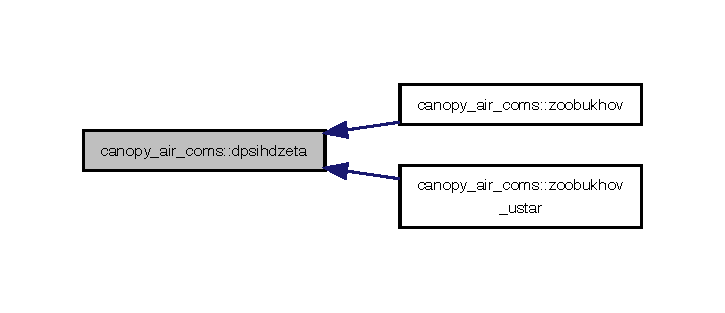
\includegraphics[width=348pt]{namespacecanopy__air__coms_a64552e0380fcb36366b5eb0f624241a3_icgraph}
\end{center}
\end{figure}
\mbox{\Hypertarget{namespacecanopy__air__coms_aa5f9649efc40a05ddc13e1450f30fad3}\label{namespacecanopy__air__coms_aa5f9649efc40a05ddc13e1450f30fad3}} 
\index{canopy\+\_\+air\+\_\+coms@{canopy\+\_\+air\+\_\+coms}!dpsihdzeta8@{dpsihdzeta8}}
\index{dpsihdzeta8@{dpsihdzeta8}!canopy\+\_\+air\+\_\+coms@{canopy\+\_\+air\+\_\+coms}}
\subsubsection{\texorpdfstring{dpsihdzeta8()}{dpsihdzeta8()}}
{\footnotesize\ttfamily real(kind=8) function canopy\+\_\+air\+\_\+coms\+::dpsihdzeta8 (\begin{DoxyParamCaption}\item[{real(kind=8), intent(in)}]{zeta,  }\item[{logical, intent(in)}]{stable }\end{DoxyParamCaption})}

Here is the caller graph for this function\+:
\nopagebreak
\begin{figure}[H]
\begin{center}
\leavevmode
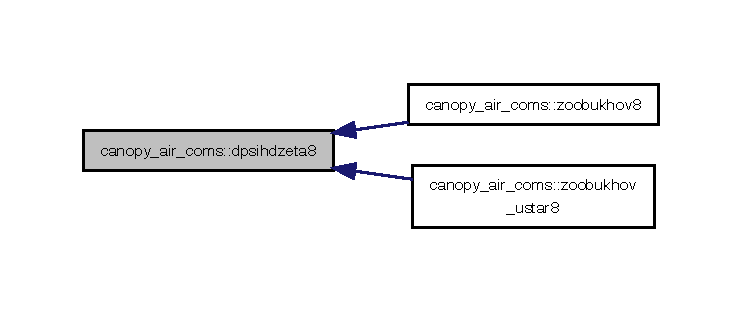
\includegraphics[width=350pt]{namespacecanopy__air__coms_aa5f9649efc40a05ddc13e1450f30fad3_icgraph}
\end{center}
\end{figure}
\mbox{\Hypertarget{namespacecanopy__air__coms_af8bc6f1d6999a4b614461cecb85c9b1b}\label{namespacecanopy__air__coms_af8bc6f1d6999a4b614461cecb85c9b1b}} 
\index{canopy\+\_\+air\+\_\+coms@{canopy\+\_\+air\+\_\+coms}!dpsimdzeta@{dpsimdzeta}}
\index{dpsimdzeta@{dpsimdzeta}!canopy\+\_\+air\+\_\+coms@{canopy\+\_\+air\+\_\+coms}}
\subsubsection{\texorpdfstring{dpsimdzeta()}{dpsimdzeta()}}
{\footnotesize\ttfamily real function canopy\+\_\+air\+\_\+coms\+::dpsimdzeta (\begin{DoxyParamCaption}\item[{real, intent(in)}]{zeta,  }\item[{logical, intent(in)}]{stable }\end{DoxyParamCaption})}

Here is the caller graph for this function\+:
\nopagebreak
\begin{figure}[H]
\begin{center}
\leavevmode
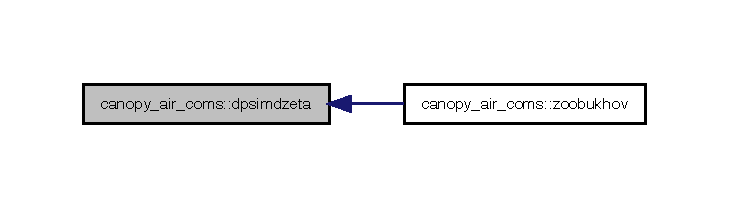
\includegraphics[width=350pt]{namespacecanopy__air__coms_af8bc6f1d6999a4b614461cecb85c9b1b_icgraph}
\end{center}
\end{figure}
\mbox{\Hypertarget{namespacecanopy__air__coms_a51b006ac118f9549aee23ddb61a1bf19}\label{namespacecanopy__air__coms_a51b006ac118f9549aee23ddb61a1bf19}} 
\index{canopy\+\_\+air\+\_\+coms@{canopy\+\_\+air\+\_\+coms}!dpsimdzeta8@{dpsimdzeta8}}
\index{dpsimdzeta8@{dpsimdzeta8}!canopy\+\_\+air\+\_\+coms@{canopy\+\_\+air\+\_\+coms}}
\subsubsection{\texorpdfstring{dpsimdzeta8()}{dpsimdzeta8()}}
{\footnotesize\ttfamily real(kind=8) function canopy\+\_\+air\+\_\+coms\+::dpsimdzeta8 (\begin{DoxyParamCaption}\item[{real(kind=8), intent(in)}]{zeta,  }\item[{logical, intent(in)}]{stable }\end{DoxyParamCaption})}

Here is the caller graph for this function\+:
\nopagebreak
\begin{figure}[H]
\begin{center}
\leavevmode
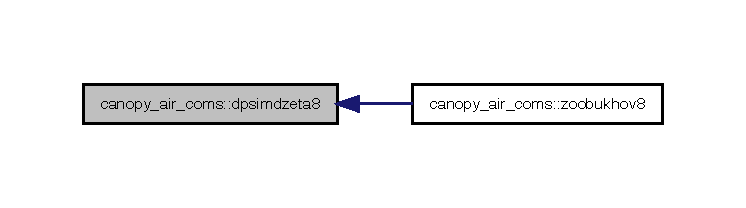
\includegraphics[width=350pt]{namespacecanopy__air__coms_a51b006ac118f9549aee23ddb61a1bf19_icgraph}
\end{center}
\end{figure}
\mbox{\Hypertarget{namespacecanopy__air__coms_acedb0f66db4b79009a69e87c5fd3ed71}\label{namespacecanopy__air__coms_acedb0f66db4b79009a69e87c5fd3ed71}} 
\index{canopy\+\_\+air\+\_\+coms@{canopy\+\_\+air\+\_\+coms}!psih@{psih}}
\index{psih@{psih}!canopy\+\_\+air\+\_\+coms@{canopy\+\_\+air\+\_\+coms}}
\subsubsection{\texorpdfstring{psih()}{psih()}}
{\footnotesize\ttfamily real function canopy\+\_\+air\+\_\+coms\+::psih (\begin{DoxyParamCaption}\item[{real, intent(in)}]{zeta,  }\item[{logical, intent(in)}]{stable }\end{DoxyParamCaption})}

Here is the caller graph for this function\+:
\nopagebreak
\begin{figure}[H]
\begin{center}
\leavevmode
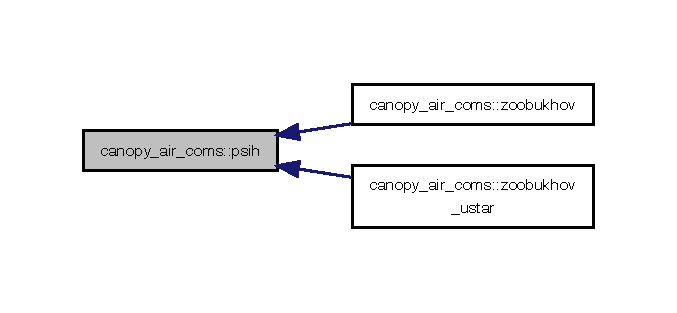
\includegraphics[width=325pt]{namespacecanopy__air__coms_acedb0f66db4b79009a69e87c5fd3ed71_icgraph}
\end{center}
\end{figure}
\mbox{\Hypertarget{namespacecanopy__air__coms_aef33f0eeea82151a8edb6dc38c4cc921}\label{namespacecanopy__air__coms_aef33f0eeea82151a8edb6dc38c4cc921}} 
\index{canopy\+\_\+air\+\_\+coms@{canopy\+\_\+air\+\_\+coms}!psih8@{psih8}}
\index{psih8@{psih8}!canopy\+\_\+air\+\_\+coms@{canopy\+\_\+air\+\_\+coms}}
\subsubsection{\texorpdfstring{psih8()}{psih8()}}
{\footnotesize\ttfamily real(kind=8) function canopy\+\_\+air\+\_\+coms\+::psih8 (\begin{DoxyParamCaption}\item[{real(kind=8), intent(in)}]{zeta,  }\item[{logical, intent(in)}]{stable }\end{DoxyParamCaption})}

Here is the caller graph for this function\+:
\nopagebreak
\begin{figure}[H]
\begin{center}
\leavevmode
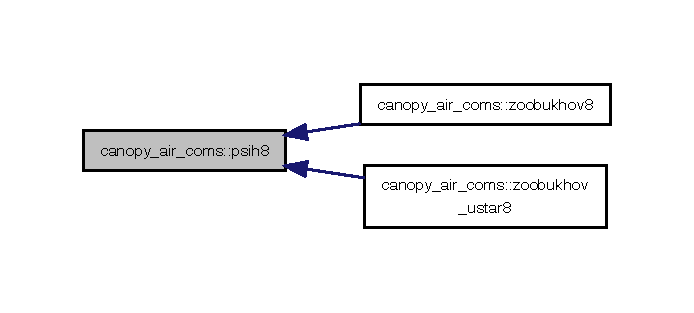
\includegraphics[width=333pt]{namespacecanopy__air__coms_aef33f0eeea82151a8edb6dc38c4cc921_icgraph}
\end{center}
\end{figure}
\mbox{\Hypertarget{namespacecanopy__air__coms_ab103fa081460babbe04c9a5a4699be5f}\label{namespacecanopy__air__coms_ab103fa081460babbe04c9a5a4699be5f}} 
\index{canopy\+\_\+air\+\_\+coms@{canopy\+\_\+air\+\_\+coms}!psim@{psim}}
\index{psim@{psim}!canopy\+\_\+air\+\_\+coms@{canopy\+\_\+air\+\_\+coms}}
\subsubsection{\texorpdfstring{psim()}{psim()}}
{\footnotesize\ttfamily real function canopy\+\_\+air\+\_\+coms\+::psim (\begin{DoxyParamCaption}\item[{real, intent(in)}]{zeta,  }\item[{logical, intent(in)}]{stable }\end{DoxyParamCaption})}

Here is the caller graph for this function\+:
\nopagebreak
\begin{figure}[H]
\begin{center}
\leavevmode
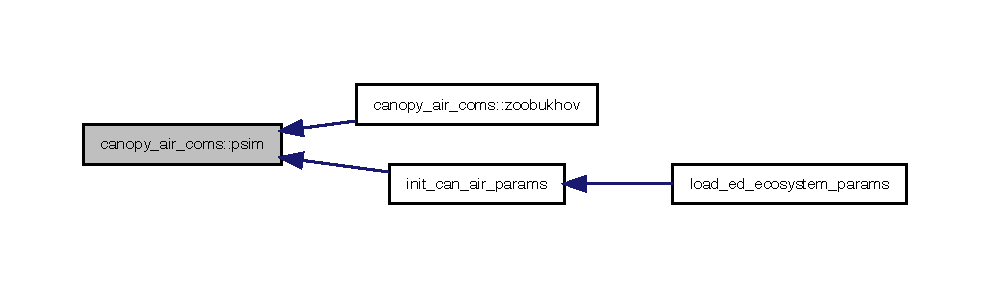
\includegraphics[width=350pt]{namespacecanopy__air__coms_ab103fa081460babbe04c9a5a4699be5f_icgraph}
\end{center}
\end{figure}
\mbox{\Hypertarget{namespacecanopy__air__coms_aba7cbe776dbfa9815870ad3686949041}\label{namespacecanopy__air__coms_aba7cbe776dbfa9815870ad3686949041}} 
\index{canopy\+\_\+air\+\_\+coms@{canopy\+\_\+air\+\_\+coms}!psim8@{psim8}}
\index{psim8@{psim8}!canopy\+\_\+air\+\_\+coms@{canopy\+\_\+air\+\_\+coms}}
\subsubsection{\texorpdfstring{psim8()}{psim8()}}
{\footnotesize\ttfamily real(kind=8) function canopy\+\_\+air\+\_\+coms\+::psim8 (\begin{DoxyParamCaption}\item[{real(kind=8), intent(in)}]{zeta,  }\item[{logical, intent(in)}]{stable }\end{DoxyParamCaption})}

Here is the caller graph for this function\+:
\nopagebreak
\begin{figure}[H]
\begin{center}
\leavevmode
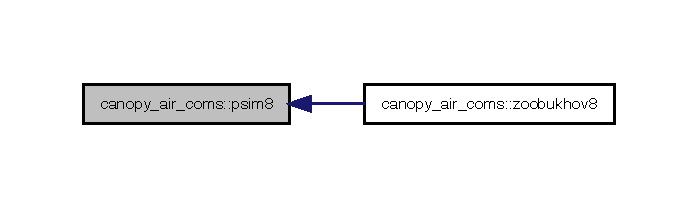
\includegraphics[width=335pt]{namespacecanopy__air__coms_aba7cbe776dbfa9815870ad3686949041_icgraph}
\end{center}
\end{figure}
\mbox{\Hypertarget{namespacecanopy__air__coms_a6062471b3381c283205ea8b27383a5e0}\label{namespacecanopy__air__coms_a6062471b3381c283205ea8b27383a5e0}} 
\index{canopy\+\_\+air\+\_\+coms@{canopy\+\_\+air\+\_\+coms}!zoobukhov@{zoobukhov}}
\index{zoobukhov@{zoobukhov}!canopy\+\_\+air\+\_\+coms@{canopy\+\_\+air\+\_\+coms}}
\subsubsection{\texorpdfstring{zoobukhov()}{zoobukhov()}}
{\footnotesize\ttfamily real function canopy\+\_\+air\+\_\+coms\+::zoobukhov (\begin{DoxyParamCaption}\item[{real, intent(in)}]{rib,  }\item[{real, intent(in)}]{zstar,  }\item[{real, intent(in)}]{rough,  }\item[{real, intent(in)}]{zoz0m,  }\item[{real, intent(in)}]{lnzoz0m,  }\item[{real, intent(in)}]{zoz0h,  }\item[{real, intent(in)}]{lnzoz0h,  }\item[{logical, intent(in)}]{stable }\end{DoxyParamCaption})}

$<$$>$$<$$>$$<$$>$$<$$>$$<$$>$$<$$>$$<$$>$$<$$>$$<$$>$$<$$>$$<$$>$$<$$>$$<$$>$$<$$>$$<$$>$$<$$>$$<$$>$$<$$>$$<$$>$$<$$>$$<$$>$$<$$>$$<$$>$$<$$>$$<$$>$$<$$>$$<$$>$$<$$>$$<$$>$$<$$>$$<$$>$$<$$>$$<$$>$$<$$>$$<$$>$$<$$>$$<$$>$$<$$>$$<$$>$$<$$>$$<$$>$$<$!

$<$$>$$<$$>$$<$$>$$<$$>$$<$$>$$<$$>$$<$$>$$<$$>$$<$$>$$<$$>$$<$$>$$<$$>$$<$$>$$<$$>$$<$$>$$<$$>$$<$$>$$<$$>$$<$$>$$<$$>$$<$$>$$<$$>$$<$$>$$<$$>$$<$$>$$<$$>$$<$$>$$<$$>$$<$$>$$<$$>$$<$$>$$<$$>$$<$$>$$<$$>$$<$$>$$<$$>$$<$$>$$<$$>$$<$$>$$<$$>$$<$$>$$<$!

$<$$>$$<$$>$$<$$>$$<$$>$$<$$>$$<$$>$$<$$>$$<$$>$$<$$>$$<$$>$$<$$>$$<$$>$$<$$>$$<$$>$$<$$>$$<$$>$$<$$>$$<$$>$$<$$>$$<$$>$$<$$>$$<$$>$$<$$>$$<$$>$$<$$>$$<$$>$$<$$>$$<$$>$$<$$>$$<$$>$$<$$>$$<$$>$$<$$>$$<$$>$$<$$>$$<$$>$$<$$>$$<$$>$$<$$>$$<$$>$$<$$>$$<$!

$<$$>$$<$$>$$<$$>$$<$$>$$<$$>$$<$$>$$<$$>$$<$$>$$<$$>$$<$$>$$<$$>$$<$$>$$<$$>$$<$$>$$<$$>$$<$$>$$<$$>$$<$$>$$<$$>$$<$$>$$<$$>$$<$$>$$<$$>$$<$$>$$<$$>$$<$$>$$<$$>$$<$$>$$<$$>$$<$$>$$<$$>$$<$$>$$<$$>$$<$$>$$<$$>$$<$$>$$<$$>$$<$$>$$<$$>$$<$$>$$<$$>$$<$!

$<$$>$$<$$>$$<$$>$$<$$>$$<$$>$$<$$>$$<$$>$$<$$>$$<$$>$$<$$>$$<$$>$$<$$>$$<$$>$$<$$>$$<$$>$$<$$>$$<$$>$$<$$>$$<$$>$$<$$>$$<$$>$$<$$>$$<$$>$$<$$>$$<$$>$$<$$>$$<$$>$$<$$>$$<$$>$$<$$>$$<$$>$$<$$>$$<$$>$$<$$>$$<$$>$$<$$>$$<$$>$$<$$>$$<$$>$$<$$>$$<$$>$$<$!

$<$$>$$<$$>$$<$$>$$<$$>$$<$$>$$<$$>$$<$$>$$<$$>$$<$$>$$<$$>$$<$$>$$<$$>$$<$$>$$<$$>$$<$$>$$<$$>$$<$$>$$<$$>$$<$$>$$<$$>$$<$$>$$<$$>$$<$$>$$<$$>$$<$$>$$<$$>$$<$$>$$<$$>$$<$$>$$<$$>$$<$$>$$<$$>$$<$$>$$<$$>$$<$$>$$<$$>$$<$$>$$<$$>$$<$$>$$<$$>$$<$$>$$<$!

$<$$>$$<$$>$$<$$>$$<$$>$$<$$>$$<$$>$$<$$>$$<$$>$$<$$>$$<$$>$$<$$>$$<$$>$$<$$>$$<$$>$$<$$>$$<$$>$$<$$>$$<$$>$$<$$>$$<$$>$$<$$>$$<$$>$$<$$>$$<$$>$$<$$>$$<$$>$$<$$>$$<$$>$$<$$>$$<$$>$$<$$>$$<$$>$$<$$>$$<$$>$$<$$>$$<$$>$$<$$>$$<$$>$$<$!

$<$$>$$<$$>$$<$$>$$<$$>$$<$$>$$<$$>$$<$$>$$<$$>$$<$$>$$<$$>$$<$$>$$<$$>$$<$$>$$<$$>$$<$$>$$<$$>$$<$$>$$<$$>$$<$$>$$<$$>$$<$$>$$<$$>$$<$$>$$<$$>$$<$$>$$<$$>$$<$$>$$<$$>$$<$$>$$<$$>$$<$$>$$<$$>$$<$$>$$<$$>$$<$$>$$<$$>$$<$$>$$<$$>$$<$!

$<$$>$$<$$>$$<$$>$$<$$>$$<$$>$$<$$>$$<$$>$$<$$>$$<$$>$$<$$>$$<$$>$$<$$>$$<$$>$$<$$>$$<$$>$$<$$>$$<$$>$$<$$>$$<$$>$$<$$>$$<$$>$$<$$>$$<$$>$$<$$>$$<$$>$$<$$>$$<$$>$$<$$>$$<$$>$$<$$>$$<$$>$$<$$>$$<$$>$$<$$>$$<$$>$$<$$>$$<$$>$$<$$>$$<$$>$$<$$>$$<$$>$$<$!

$<$$>$$<$$>$$<$$>$$<$$>$$<$$>$$<$$>$$<$$>$$<$$>$$<$$>$$<$$>$$<$$>$$<$$>$$<$$>$$<$$>$$<$$>$$<$$>$$<$$>$$<$$>$$<$$>$$<$$>$$<$$>$$<$$>$$<$$>$$<$$>$$<$$>$$<$$>$$<$$>$$<$$>$$<$$>$$<$$>$$<$$>$$<$$>$$<$$>$$<$$>$$<$$>$$<$$>$$<$$>$$<$$>$$<$$>$$<$$>$$<$$>$$<$! Here is the call graph for this function\+:
\nopagebreak
\begin{figure}[H]
\begin{center}
\leavevmode
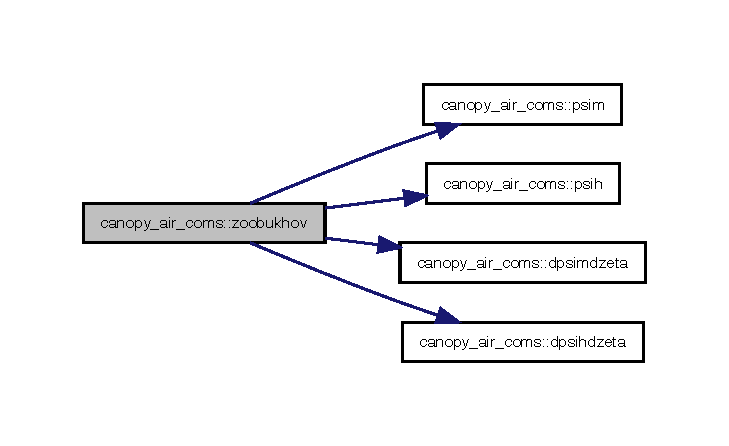
\includegraphics[width=350pt]{namespacecanopy__air__coms_a6062471b3381c283205ea8b27383a5e0_cgraph}
\end{center}
\end{figure}
\mbox{\Hypertarget{namespacecanopy__air__coms_afef697305b4b30385c5206f48d9e787c}\label{namespacecanopy__air__coms_afef697305b4b30385c5206f48d9e787c}} 
\index{canopy\+\_\+air\+\_\+coms@{canopy\+\_\+air\+\_\+coms}!zoobukhov8@{zoobukhov8}}
\index{zoobukhov8@{zoobukhov8}!canopy\+\_\+air\+\_\+coms@{canopy\+\_\+air\+\_\+coms}}
\subsubsection{\texorpdfstring{zoobukhov8()}{zoobukhov8()}}
{\footnotesize\ttfamily real(kind=8) function canopy\+\_\+air\+\_\+coms\+::zoobukhov8 (\begin{DoxyParamCaption}\item[{real(kind=8), intent(in)}]{rib,  }\item[{real(kind=8), intent(in)}]{zstar,  }\item[{real(kind=8), intent(in)}]{rough,  }\item[{real(kind=8), intent(in)}]{zoz0m,  }\item[{real(kind=8), intent(in)}]{lnzoz0m,  }\item[{real(kind=8), intent(in)}]{zoz0h,  }\item[{real(kind=8), intent(in)}]{lnzoz0h,  }\item[{logical, intent(in)}]{stable }\end{DoxyParamCaption})}

$<$$>$$<$$>$$<$$>$$<$$>$$<$$>$$<$$>$$<$$>$$<$$>$$<$$>$$<$$>$$<$$>$$<$$>$$<$$>$$<$$>$$<$$>$$<$$>$$<$$>$$<$$>$$<$$>$$<$$>$$<$$>$$<$$>$$<$$>$$<$$>$$<$$>$$<$$>$$<$$>$$<$$>$$<$$>$$<$$>$$<$$>$$<$$>$$<$$>$$<$$>$$<$$>$$<$$>$$<$$>$$<$$>$$<$$>$$<$$>$$<$$>$$<$!

$<$$>$$<$$>$$<$$>$$<$$>$$<$$>$$<$$>$$<$$>$$<$$>$$<$$>$$<$$>$$<$$>$$<$$>$$<$$>$$<$$>$$<$$>$$<$$>$$<$$>$$<$$>$$<$$>$$<$$>$$<$$>$$<$$>$$<$$>$$<$$>$$<$$>$$<$$>$$<$$>$$<$$>$$<$$>$$<$$>$$<$$>$$<$$>$$<$$>$$<$$>$$<$$>$$<$$>$$<$$>$$<$$>$$<$$>$$<$$>$$<$$>$$<$!

$<$$>$$<$$>$$<$$>$$<$$>$$<$$>$$<$$>$$<$$>$$<$$>$$<$$>$$<$$>$$<$$>$$<$$>$$<$$>$$<$$>$$<$$>$$<$$>$$<$$>$$<$$>$$<$$>$$<$$>$$<$$>$$<$$>$$<$$>$$<$$>$$<$$>$$<$$>$$<$$>$$<$$>$$<$$>$$<$$>$$<$$>$$<$$>$$<$$>$$<$$>$$<$$>$$<$$>$$<$$>$$<$$>$$<$$>$$<$$>$$<$$>$$<$!

$<$$>$$<$$>$$<$$>$$<$$>$$<$$>$$<$$>$$<$$>$$<$$>$$<$$>$$<$$>$$<$$>$$<$$>$$<$$>$$<$$>$$<$$>$$<$$>$$<$$>$$<$$>$$<$$>$$<$$>$$<$$>$$<$$>$$<$$>$$<$$>$$<$$>$$<$$>$$<$$>$$<$$>$$<$$>$$<$$>$$<$$>$$<$$>$$<$$>$$<$$>$$<$$>$$<$$>$$<$$>$$<$$>$$<$$>$$<$$>$$<$$>$$<$!

$<$$>$$<$$>$$<$$>$$<$$>$$<$$>$$<$$>$$<$$>$$<$$>$$<$$>$$<$$>$$<$$>$$<$$>$$<$$>$$<$$>$$<$$>$$<$$>$$<$$>$$<$$>$$<$$>$$<$$>$$<$$>$$<$$>$$<$$>$$<$$>$$<$$>$$<$$>$$<$$>$$<$$>$$<$$>$$<$$>$$<$$>$$<$$>$$<$$>$$<$$>$$<$$>$$<$$>$$<$$>$$<$$>$$<$$>$$<$$>$$<$$>$$<$!

$<$$>$$<$$>$$<$$>$$<$$>$$<$$>$$<$$>$$<$$>$$<$$>$$<$$>$$<$$>$$<$$>$$<$$>$$<$$>$$<$$>$$<$$>$$<$$>$$<$$>$$<$$>$$<$$>$$<$$>$$<$$>$$<$$>$$<$$>$$<$$>$$<$$>$$<$$>$$<$$>$$<$$>$$<$$>$$<$$>$$<$$>$$<$$>$$<$$>$$<$$>$$<$$>$$<$$>$$<$$>$$<$$>$$<$$>$$<$$>$$<$$>$$<$!

$<$$>$$<$$>$$<$$>$$<$$>$$<$$>$$<$$>$$<$$>$$<$$>$$<$$>$$<$$>$$<$$>$$<$$>$$<$$>$$<$$>$$<$$>$$<$$>$$<$$>$$<$$>$$<$$>$$<$$>$$<$$>$$<$$>$$<$$>$$<$$>$$<$$>$$<$$>$$<$$>$$<$$>$$<$$>$$<$$>$$<$$>$$<$$>$$<$$>$$<$$>$$<$$>$$<$$>$$<$$>$$<$$>$$<$!

$<$$>$$<$$>$$<$$>$$<$$>$$<$$>$$<$$>$$<$$>$$<$$>$$<$$>$$<$$>$$<$$>$$<$$>$$<$$>$$<$$>$$<$$>$$<$$>$$<$$>$$<$$>$$<$$>$$<$$>$$<$$>$$<$$>$$<$$>$$<$$>$$<$$>$$<$$>$$<$$>$$<$$>$$<$$>$$<$$>$$<$$>$$<$$>$$<$$>$$<$$>$$<$$>$$<$$>$$<$$>$$<$$>$$<$!

$<$$>$$<$$>$$<$$>$$<$$>$$<$$>$$<$$>$$<$$>$$<$$>$$<$$>$$<$$>$$<$$>$$<$$>$$<$$>$$<$$>$$<$$>$$<$$>$$<$$>$$<$$>$$<$$>$$<$$>$$<$$>$$<$$>$$<$$>$$<$$>$$<$$>$$<$$>$$<$$>$$<$$>$$<$$>$$<$$>$$<$$>$$<$$>$$<$$>$$<$$>$$<$$>$$<$$>$$<$$>$$<$$>$$<$$>$$<$$>$$<$$>$$<$!

$<$$>$$<$$>$$<$$>$$<$$>$$<$$>$$<$$>$$<$$>$$<$$>$$<$$>$$<$$>$$<$$>$$<$$>$$<$$>$$<$$>$$<$$>$$<$$>$$<$$>$$<$$>$$<$$>$$<$$>$$<$$>$$<$$>$$<$$>$$<$$>$$<$$>$$<$$>$$<$$>$$<$$>$$<$$>$$<$$>$$<$$>$$<$$>$$<$$>$$<$$>$$<$$>$$<$$>$$<$$>$$<$$>$$<$$>$$<$$>$$<$$>$$<$! Here is the call graph for this function\+:
\nopagebreak
\begin{figure}[H]
\begin{center}
\leavevmode
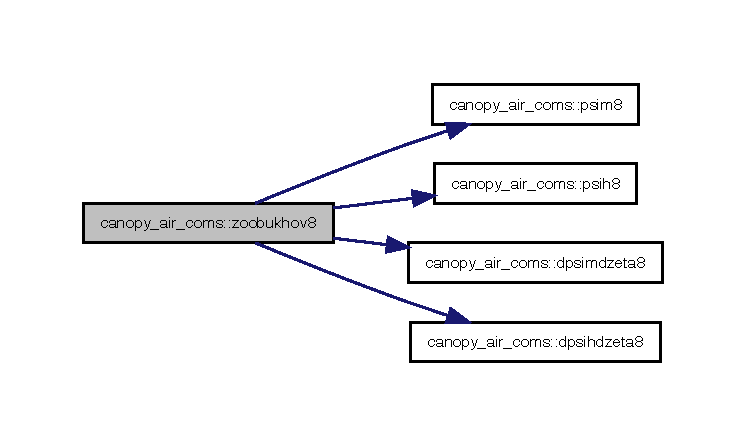
\includegraphics[width=350pt]{namespacecanopy__air__coms_afef697305b4b30385c5206f48d9e787c_cgraph}
\end{center}
\end{figure}
\mbox{\Hypertarget{namespacecanopy__air__coms_a5251266695c581c8f4058d98f6c86200}\label{namespacecanopy__air__coms_a5251266695c581c8f4058d98f6c86200}} 
\index{canopy\+\_\+air\+\_\+coms@{canopy\+\_\+air\+\_\+coms}!zoobukhov\+\_\+ustar@{zoobukhov\+\_\+ustar}}
\index{zoobukhov\+\_\+ustar@{zoobukhov\+\_\+ustar}!canopy\+\_\+air\+\_\+coms@{canopy\+\_\+air\+\_\+coms}}
\subsubsection{\texorpdfstring{zoobukhov\+\_\+ustar()}{zoobukhov\_ustar()}}
{\footnotesize\ttfamily real function canopy\+\_\+air\+\_\+coms\+::zoobukhov\+\_\+ustar (\begin{DoxyParamCaption}\item[{real(kind=4), intent(in)}]{rib,  }\item[{real(kind=4), intent(in)}]{zstar,  }\item[{real(kind=4), intent(in)}]{rough,  }\item[{real(kind=4), intent(in)}]{zoz0h,  }\item[{real(kind=4), intent(in)}]{lnzoz0h,  }\item[{real(kind=4), intent(in)}]{kuoustar,  }\item[{logical, intent(in)}]{stable }\end{DoxyParamCaption})}

$<$$>$$<$$>$$<$$>$$<$$>$$<$$>$$<$$>$$<$$>$$<$$>$$<$$>$$<$$>$$<$$>$$<$$>$$<$$>$$<$$>$$<$$>$$<$$>$$<$$>$$<$$>$$<$$>$$<$$>$$<$$>$$<$$>$$<$$>$$<$$>$$<$$>$$<$$>$$<$$>$$<$$>$$<$$>$$<$$>$$<$$>$$<$$>$$<$$>$$<$$>$$<$$>$$<$$>$$<$$>$$<$$>$$<$$>$$<$$>$$<$$>$$<$!

$<$$>$$<$$>$$<$$>$$<$$>$$<$$>$$<$$>$$<$$>$$<$$>$$<$$>$$<$$>$$<$$>$$<$$>$$<$$>$$<$$>$$<$$>$$<$$>$$<$$>$$<$$>$$<$$>$$<$$>$$<$$>$$<$$>$$<$$>$$<$$>$$<$$>$$<$$>$$<$$>$$<$$>$$<$$>$$<$$>$$<$$>$$<$$>$$<$$>$$<$$>$$<$$>$$<$$>$$<$$>$$<$$>$$<$$>$$<$$>$$<$$>$$<$!

$<$$>$$<$$>$$<$$>$$<$$>$$<$$>$$<$$>$$<$$>$$<$$>$$<$$>$$<$$>$$<$$>$$<$$>$$<$$>$$<$$>$$<$$>$$<$$>$$<$$>$$<$$>$$<$$>$$<$$>$$<$$>$$<$$>$$<$$>$$<$$>$$<$$>$$<$$>$$<$$>$$<$$>$$<$$>$$<$$>$$<$$>$$<$$>$$<$$>$$<$$>$$<$$>$$<$$>$$<$$>$$<$$>$$<$$>$$<$$>$$<$$>$$<$!

$<$$>$$<$$>$$<$$>$$<$$>$$<$$>$$<$$>$$<$$>$$<$$>$$<$$>$$<$$>$$<$$>$$<$$>$$<$$>$$<$$>$$<$$>$$<$$>$$<$$>$$<$$>$$<$$>$$<$$>$$<$$>$$<$$>$$<$$>$$<$$>$$<$$>$$<$$>$$<$$>$$<$$>$$<$$>$$<$$>$$<$$>$$<$$>$$<$$>$$<$$>$$<$$>$$<$$>$$<$$>$$<$$>$$<$$>$$<$$>$$<$$>$$<$!

$<$$>$$<$$>$$<$$>$$<$$>$$<$$>$$<$$>$$<$$>$$<$$>$$<$$>$$<$$>$$<$$>$$<$$>$$<$$>$$<$$>$$<$$>$$<$$>$$<$$>$$<$$>$$<$$>$$<$$>$$<$$>$$<$$>$$<$$>$$<$$>$$<$$>$$<$$>$$<$$>$$<$$>$$<$$>$$<$$>$$<$$>$$<$$>$$<$$>$$<$$>$$<$$>$$<$$>$$<$$>$$<$$>$$<$$>$$<$$>$$<$$>$$<$!

$<$$>$$<$$>$$<$$>$$<$$>$$<$$>$$<$$>$$<$$>$$<$$>$$<$$>$$<$$>$$<$$>$$<$$>$$<$$>$$<$$>$$<$$>$$<$$>$$<$$>$$<$$>$$<$$>$$<$$>$$<$$>$$<$$>$$<$$>$$<$$>$$<$$>$$<$$>$$<$$>$$<$$>$$<$$>$$<$$>$$<$$>$$<$$>$$<$$>$$<$$>$$<$$>$$<$$>$$<$$>$$<$$>$$<$$>$$<$$>$$<$$>$$<$!

$<$$>$$<$$>$$<$$>$$<$$>$$<$$>$$<$$>$$<$$>$$<$$>$$<$$>$$<$$>$$<$$>$$<$$>$$<$$>$$<$$>$$<$$>$$<$$>$$<$$>$$<$$>$$<$$>$$<$$>$$<$$>$$<$$>$$<$$>$$<$$>$$<$$>$$<$$>$$<$$>$$<$$>$$<$$>$$<$$>$$<$$>$$<$$>$$<$$>$$<$$>$$<$$>$$<$$>$$<$$>$$<$$>$$<$!

$<$$>$$<$$>$$<$$>$$<$$>$$<$$>$$<$$>$$<$$>$$<$$>$$<$$>$$<$$>$$<$$>$$<$$>$$<$$>$$<$$>$$<$$>$$<$$>$$<$$>$$<$$>$$<$$>$$<$$>$$<$$>$$<$$>$$<$$>$$<$$>$$<$$>$$<$$>$$<$$>$$<$$>$$<$$>$$<$$>$$<$$>$$<$$>$$<$$>$$<$$>$$<$$>$$<$$>$$<$$>$$<$$>$$<$!

$<$$>$$<$$>$$<$$>$$<$$>$$<$$>$$<$$>$$<$$>$$<$$>$$<$$>$$<$$>$$<$$>$$<$$>$$<$$>$$<$$>$$<$$>$$<$$>$$<$$>$$<$$>$$<$$>$$<$$>$$<$$>$$<$$>$$<$$>$$<$$>$$<$$>$$<$$>$$<$$>$$<$$>$$<$$>$$<$$>$$<$$>$$<$$>$$<$$>$$<$$>$$<$$>$$<$$>$$<$$>$$<$$>$$<$$>$$<$$>$$<$$>$$<$!

$<$$>$$<$$>$$<$$>$$<$$>$$<$$>$$<$$>$$<$$>$$<$$>$$<$$>$$<$$>$$<$$>$$<$$>$$<$$>$$<$$>$$<$$>$$<$$>$$<$$>$$<$$>$$<$$>$$<$$>$$<$$>$$<$$>$$<$$>$$<$$>$$<$$>$$<$$>$$<$$>$$<$$>$$<$$>$$<$$>$$<$$>$$<$$>$$<$$>$$<$$>$$<$$>$$<$$>$$<$$>$$<$$>$$<$$>$$<$$>$$<$$>$$<$! Here is the call graph for this function\+:
\nopagebreak
\begin{figure}[H]
\begin{center}
\leavevmode
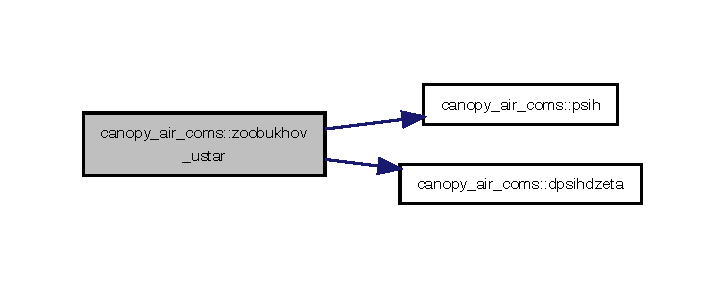
\includegraphics[width=348pt]{namespacecanopy__air__coms_a5251266695c581c8f4058d98f6c86200_cgraph}
\end{center}
\end{figure}
\mbox{\Hypertarget{namespacecanopy__air__coms_a6ef582f46fded1355973730e6a2289f2}\label{namespacecanopy__air__coms_a6ef582f46fded1355973730e6a2289f2}} 
\index{canopy\+\_\+air\+\_\+coms@{canopy\+\_\+air\+\_\+coms}!zoobukhov\+\_\+ustar8@{zoobukhov\+\_\+ustar8}}
\index{zoobukhov\+\_\+ustar8@{zoobukhov\+\_\+ustar8}!canopy\+\_\+air\+\_\+coms@{canopy\+\_\+air\+\_\+coms}}
\subsubsection{\texorpdfstring{zoobukhov\+\_\+ustar8()}{zoobukhov\_ustar8()}}
{\footnotesize\ttfamily real(kind=8) function canopy\+\_\+air\+\_\+coms\+::zoobukhov\+\_\+ustar8 (\begin{DoxyParamCaption}\item[{real(kind=8), intent(in)}]{rib,  }\item[{real(kind=8), intent(in)}]{zstar,  }\item[{real(kind=8), intent(in)}]{rough,  }\item[{real(kind=8), intent(in)}]{zoz0h,  }\item[{real(kind=8), intent(in)}]{lnzoz0h,  }\item[{real(kind=8), intent(in)}]{kuoustar,  }\item[{logical, intent(in)}]{stable }\end{DoxyParamCaption})}

$<$$>$$<$$>$$<$$>$$<$$>$$<$$>$$<$$>$$<$$>$$<$$>$$<$$>$$<$$>$$<$$>$$<$$>$$<$$>$$<$$>$$<$$>$$<$$>$$<$$>$$<$$>$$<$$>$$<$$>$$<$$>$$<$$>$$<$$>$$<$$>$$<$$>$$<$$>$$<$$>$$<$$>$$<$$>$$<$$>$$<$$>$$<$$>$$<$$>$$<$$>$$<$$>$$<$$>$$<$$>$$<$$>$$<$$>$$<$$>$$<$$>$$<$!

$<$$>$$<$$>$$<$$>$$<$$>$$<$$>$$<$$>$$<$$>$$<$$>$$<$$>$$<$$>$$<$$>$$<$$>$$<$$>$$<$$>$$<$$>$$<$$>$$<$$>$$<$$>$$<$$>$$<$$>$$<$$>$$<$$>$$<$$>$$<$$>$$<$$>$$<$$>$$<$$>$$<$$>$$<$$>$$<$$>$$<$$>$$<$$>$$<$$>$$<$$>$$<$$>$$<$$>$$<$$>$$<$$>$$<$$>$$<$$>$$<$$>$$<$!

$<$$>$$<$$>$$<$$>$$<$$>$$<$$>$$<$$>$$<$$>$$<$$>$$<$$>$$<$$>$$<$$>$$<$$>$$<$$>$$<$$>$$<$$>$$<$$>$$<$$>$$<$$>$$<$$>$$<$$>$$<$$>$$<$$>$$<$$>$$<$$>$$<$$>$$<$$>$$<$$>$$<$$>$$<$$>$$<$$>$$<$$>$$<$$>$$<$$>$$<$$>$$<$$>$$<$$>$$<$$>$$<$$>$$<$$>$$<$$>$$<$$>$$<$!

$<$$>$$<$$>$$<$$>$$<$$>$$<$$>$$<$$>$$<$$>$$<$$>$$<$$>$$<$$>$$<$$>$$<$$>$$<$$>$$<$$>$$<$$>$$<$$>$$<$$>$$<$$>$$<$$>$$<$$>$$<$$>$$<$$>$$<$$>$$<$$>$$<$$>$$<$$>$$<$$>$$<$$>$$<$$>$$<$$>$$<$$>$$<$$>$$<$$>$$<$$>$$<$$>$$<$$>$$<$$>$$<$$>$$<$$>$$<$$>$$<$$>$$<$!

$<$$>$$<$$>$$<$$>$$<$$>$$<$$>$$<$$>$$<$$>$$<$$>$$<$$>$$<$$>$$<$$>$$<$$>$$<$$>$$<$$>$$<$$>$$<$$>$$<$$>$$<$$>$$<$$>$$<$$>$$<$$>$$<$$>$$<$$>$$<$$>$$<$$>$$<$$>$$<$$>$$<$$>$$<$$>$$<$$>$$<$$>$$<$$>$$<$$>$$<$$>$$<$$>$$<$$>$$<$$>$$<$$>$$<$$>$$<$$>$!

$<$$>$$<$$>$$<$$>$$<$$>$$<$$>$$<$$>$$<$$>$$<$$>$$<$$>$$<$$>$$<$$>$$<$$>$$<$$>$$<$$>$$<$$>$$<$$>$$<$$>$$<$$>$$<$$>$$<$$>$$<$$>$$<$$>$$<$$>$$<$$>$$<$$>$$<$$>$$<$$>$$<$$>$$<$$>$$<$$>$$<$$>$$<$$>$$<$$>$$<$$>$$<$$>$$<$$>$$<$$>$$<$$>$$<$$>$$<$$>$!

$<$$>$$<$$>$$<$$>$$<$$>$$<$$>$$<$$>$$<$$>$$<$$>$$<$$>$$<$$>$$<$$>$$<$$>$$<$$>$$<$$>$$<$$>$$<$$>$$<$$>$$<$$>$$<$$>$$<$$>$$<$$>$$<$$>$$<$$>$$<$$>$$<$$>$$<$$>$$<$$>$$<$$>$$<$$>$$<$$>$$<$$>$$<$$>$$<$$>$$<$$>$$<$$>$$<$$>$$<$$>$$<$$>$$<$!

$<$$>$$<$$>$$<$$>$$<$$>$$<$$>$$<$$>$$<$$>$$<$$>$$<$$>$$<$$>$$<$$>$$<$$>$$<$$>$$<$$>$$<$$>$$<$$>$$<$$>$$<$$>$$<$$>$$<$$>$$<$$>$$<$$>$$<$$>$$<$$>$$<$$>$$<$$>$$<$$>$$<$$>$$<$$>$$<$$>$$<$$>$$<$$>$$<$$>$$<$$>$$<$$>$$<$$>$$<$$>$$<$$>$$<$!

$<$$>$$<$$>$$<$$>$$<$$>$$<$$>$$<$$>$$<$$>$$<$$>$$<$$>$$<$$>$$<$$>$$<$$>$$<$$>$$<$$>$$<$$>$$<$$>$$<$$>$$<$$>$$<$$>$$<$$>$$<$$>$$<$$>$$<$$>$$<$$>$$<$$>$$<$$>$$<$$>$$<$$>$$<$$>$$<$$>$$<$$>$$<$$>$$<$$>$$<$$>$$<$$>$$<$$>$$<$$>$$<$$>$$<$$>$$<$$>$!

$<$$>$$<$$>$$<$$>$$<$$>$$<$$>$$<$$>$$<$$>$$<$$>$$<$$>$$<$$>$$<$$>$$<$$>$$<$$>$$<$$>$$<$$>$$<$$>$$<$$>$$<$$>$$<$$>$$<$$>$$<$$>$$<$$>$$<$$>$$<$$>$$<$$>$$<$$>$$<$$>$$<$$>$$<$$>$$<$$>$$<$$>$$<$$>$$<$$>$$<$$>$$<$$>$$<$$>$$<$$>$$<$$>$$<$$>$$<$$>$!

$<$$>$$<$$>$$<$$>$$<$$>$$<$$>$$<$$>$$<$$>$$<$$>$$<$$>$$<$$>$$<$$>$$<$$>$$<$$>$$<$$>$$<$$>$$<$$>$$<$$>$$<$$>$$<$$>$$<$$>$$<$$>$$<$$>$$<$$>$$<$$>$$<$$>$$<$$>$$<$$>$$<$$>$$<$$>$$<$$>$$<$$>$$<$$>$$<$$>$$<$$>$$<$$>$$<$$>$$<$$>$$<$$>$$<$$>$$<$$>$!

$<$$>$$<$$>$$<$$>$$<$$>$$<$$>$$<$$>$$<$$>$$<$$>$$<$$>$$<$$>$$<$$>$$<$$>$$<$$>$$<$$>$$<$$>$$<$$>$$<$$>$$<$$>$$<$$>$$<$$>$$<$$>$$<$$>$$<$$>$$<$$>$$<$$>$$<$$>$$<$$>$$<$$>$$<$$>$$<$$>$$<$$>$$<$$>$$<$$>$$<$$>$$<$$>$$<$$>$$<$$>$$<$$>$$<$$>$$<$$>$! Here is the call graph for this function\+:
\nopagebreak
\begin{figure}[H]
\begin{center}
\leavevmode
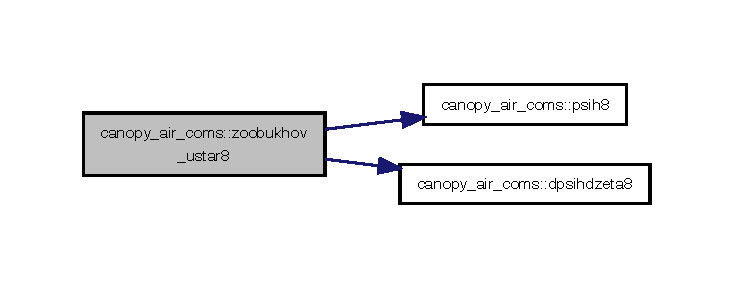
\includegraphics[width=350pt]{namespacecanopy__air__coms_a6ef582f46fded1355973730e6a2289f2_cgraph}
\end{center}
\end{figure}


\subsection{Variable Documentation}
\mbox{\Hypertarget{namespacecanopy__air__coms_a8943107817bd72a2ecf2c8ac35516efc}\label{namespacecanopy__air__coms_a8943107817bd72a2ecf2c8ac35516efc}} 
\index{canopy\+\_\+air\+\_\+coms@{canopy\+\_\+air\+\_\+coms}!abh91@{abh91}}
\index{abh91@{abh91}!canopy\+\_\+air\+\_\+coms@{canopy\+\_\+air\+\_\+coms}}
\subsubsection{\texorpdfstring{abh91}{abh91}}
{\footnotesize\ttfamily real canopy\+\_\+air\+\_\+coms\+::abh91}

\mbox{\Hypertarget{namespacecanopy__air__coms_a7bbc194838f911d2e8b0948159f4d62e}\label{namespacecanopy__air__coms_a7bbc194838f911d2e8b0948159f4d62e}} 
\index{canopy\+\_\+air\+\_\+coms@{canopy\+\_\+air\+\_\+coms}!abh918@{abh918}}
\index{abh918@{abh918}!canopy\+\_\+air\+\_\+coms@{canopy\+\_\+air\+\_\+coms}}
\subsubsection{\texorpdfstring{abh918}{abh918}}
{\footnotesize\ttfamily real(kind=8) canopy\+\_\+air\+\_\+coms\+::abh918}

\mbox{\Hypertarget{namespacecanopy__air__coms_a910e0e75420e6cd46075062c7da2b565}\label{namespacecanopy__air__coms_a910e0e75420e6cd46075062c7da2b565}} 
\index{canopy\+\_\+air\+\_\+coms@{canopy\+\_\+air\+\_\+coms}!acyli\+\_\+lami@{acyli\+\_\+lami}}
\index{acyli\+\_\+lami@{acyli\+\_\+lami}!canopy\+\_\+air\+\_\+coms@{canopy\+\_\+air\+\_\+coms}}
\subsubsection{\texorpdfstring{acyli\+\_\+lami}{acyli\_lami}}
{\footnotesize\ttfamily real(kind=4) canopy\+\_\+air\+\_\+coms\+::acyli\+\_\+lami}

\mbox{\Hypertarget{namespacecanopy__air__coms_a325f601d72eb729cc4301008156be76b}\label{namespacecanopy__air__coms_a325f601d72eb729cc4301008156be76b}} 
\index{canopy\+\_\+air\+\_\+coms@{canopy\+\_\+air\+\_\+coms}!acyli\+\_\+lami8@{acyli\+\_\+lami8}}
\index{acyli\+\_\+lami8@{acyli\+\_\+lami8}!canopy\+\_\+air\+\_\+coms@{canopy\+\_\+air\+\_\+coms}}
\subsubsection{\texorpdfstring{acyli\+\_\+lami8}{acyli\_lami8}}
{\footnotesize\ttfamily real(kind=8) canopy\+\_\+air\+\_\+coms\+::acyli\+\_\+lami8}

\mbox{\Hypertarget{namespacecanopy__air__coms_a42c5385303996a52e2fce111d922eaf2}\label{namespacecanopy__air__coms_a42c5385303996a52e2fce111d922eaf2}} 
\index{canopy\+\_\+air\+\_\+coms@{canopy\+\_\+air\+\_\+coms}!acyli\+\_\+turb@{acyli\+\_\+turb}}
\index{acyli\+\_\+turb@{acyli\+\_\+turb}!canopy\+\_\+air\+\_\+coms@{canopy\+\_\+air\+\_\+coms}}
\subsubsection{\texorpdfstring{acyli\+\_\+turb}{acyli\_turb}}
{\footnotesize\ttfamily real(kind=4) canopy\+\_\+air\+\_\+coms\+::acyli\+\_\+turb}

\mbox{\Hypertarget{namespacecanopy__air__coms_a933920d4f406fd57c33f8cef1ca8bb83}\label{namespacecanopy__air__coms_a933920d4f406fd57c33f8cef1ca8bb83}} 
\index{canopy\+\_\+air\+\_\+coms@{canopy\+\_\+air\+\_\+coms}!acyli\+\_\+turb8@{acyli\+\_\+turb8}}
\index{acyli\+\_\+turb8@{acyli\+\_\+turb8}!canopy\+\_\+air\+\_\+coms@{canopy\+\_\+air\+\_\+coms}}
\subsubsection{\texorpdfstring{acyli\+\_\+turb8}{acyli\_turb8}}
{\footnotesize\ttfamily real(kind=8) canopy\+\_\+air\+\_\+coms\+::acyli\+\_\+turb8}

\mbox{\Hypertarget{namespacecanopy__air__coms_a478fe27fc0f34c4b09208d0f99bae8e5}\label{namespacecanopy__air__coms_a478fe27fc0f34c4b09208d0f99bae8e5}} 
\index{canopy\+\_\+air\+\_\+coms@{canopy\+\_\+air\+\_\+coms}!aflat\+\_\+lami@{aflat\+\_\+lami}}
\index{aflat\+\_\+lami@{aflat\+\_\+lami}!canopy\+\_\+air\+\_\+coms@{canopy\+\_\+air\+\_\+coms}}
\subsubsection{\texorpdfstring{aflat\+\_\+lami}{aflat\_lami}}
{\footnotesize\ttfamily real(kind=4) canopy\+\_\+air\+\_\+coms\+::aflat\+\_\+lami}

\mbox{\Hypertarget{namespacecanopy__air__coms_af642ae1aafe80d1c6e7fde278a2236df}\label{namespacecanopy__air__coms_af642ae1aafe80d1c6e7fde278a2236df}} 
\index{canopy\+\_\+air\+\_\+coms@{canopy\+\_\+air\+\_\+coms}!aflat\+\_\+lami8@{aflat\+\_\+lami8}}
\index{aflat\+\_\+lami8@{aflat\+\_\+lami8}!canopy\+\_\+air\+\_\+coms@{canopy\+\_\+air\+\_\+coms}}
\subsubsection{\texorpdfstring{aflat\+\_\+lami8}{aflat\_lami8}}
{\footnotesize\ttfamily real(kind=8) canopy\+\_\+air\+\_\+coms\+::aflat\+\_\+lami8}

\mbox{\Hypertarget{namespacecanopy__air__coms_a63aa3cee74a44dfccdad43b566c7149c}\label{namespacecanopy__air__coms_a63aa3cee74a44dfccdad43b566c7149c}} 
\index{canopy\+\_\+air\+\_\+coms@{canopy\+\_\+air\+\_\+coms}!aflat\+\_\+turb@{aflat\+\_\+turb}}
\index{aflat\+\_\+turb@{aflat\+\_\+turb}!canopy\+\_\+air\+\_\+coms@{canopy\+\_\+air\+\_\+coms}}
\subsubsection{\texorpdfstring{aflat\+\_\+turb}{aflat\_turb}}
{\footnotesize\ttfamily real(kind=4) canopy\+\_\+air\+\_\+coms\+::aflat\+\_\+turb}

\mbox{\Hypertarget{namespacecanopy__air__coms_a74069fab7440b8c4adf33de11779b980}\label{namespacecanopy__air__coms_a74069fab7440b8c4adf33de11779b980}} 
\index{canopy\+\_\+air\+\_\+coms@{canopy\+\_\+air\+\_\+coms}!aflat\+\_\+turb8@{aflat\+\_\+turb8}}
\index{aflat\+\_\+turb8@{aflat\+\_\+turb8}!canopy\+\_\+air\+\_\+coms@{canopy\+\_\+air\+\_\+coms}}
\subsubsection{\texorpdfstring{aflat\+\_\+turb8}{aflat\_turb8}}
{\footnotesize\ttfamily real(kind=8) canopy\+\_\+air\+\_\+coms\+::aflat\+\_\+turb8}

\mbox{\Hypertarget{namespacecanopy__air__coms_ac16bf823a6fc81f0d671fa06ca5de7e7}\label{namespacecanopy__air__coms_ac16bf823a6fc81f0d671fa06ca5de7e7}} 
\index{canopy\+\_\+air\+\_\+coms@{canopy\+\_\+air\+\_\+coms}!alpha\+\_\+m97@{alpha\+\_\+m97}}
\index{alpha\+\_\+m97@{alpha\+\_\+m97}!canopy\+\_\+air\+\_\+coms@{canopy\+\_\+air\+\_\+coms}}
\subsubsection{\texorpdfstring{alpha\+\_\+m97}{alpha\_m97}}
{\footnotesize\ttfamily real(kind=4) canopy\+\_\+air\+\_\+coms\+::alpha\+\_\+m97}

\mbox{\Hypertarget{namespacecanopy__air__coms_aaca98abaf4f4ff986bd24a7e1ceea8a6}\label{namespacecanopy__air__coms_aaca98abaf4f4ff986bd24a7e1ceea8a6}} 
\index{canopy\+\_\+air\+\_\+coms@{canopy\+\_\+air\+\_\+coms}!alpha\+\_\+m97\+\_\+8@{alpha\+\_\+m97\+\_\+8}}
\index{alpha\+\_\+m97\+\_\+8@{alpha\+\_\+m97\+\_\+8}!canopy\+\_\+air\+\_\+coms@{canopy\+\_\+air\+\_\+coms}}
\subsubsection{\texorpdfstring{alpha\+\_\+m97\+\_\+8}{alpha\_m97\_8}}
{\footnotesize\ttfamily real(kind=8) canopy\+\_\+air\+\_\+coms\+::alpha\+\_\+m97\+\_\+8}

\mbox{\Hypertarget{namespacecanopy__air__coms_aee71b7396b4019638189e8d16f29d5bc}\label{namespacecanopy__air__coms_aee71b7396b4019638189e8d16f29d5bc}} 
\index{canopy\+\_\+air\+\_\+coms@{canopy\+\_\+air\+\_\+coms}!alpha\+\_\+mw99@{alpha\+\_\+mw99}}
\index{alpha\+\_\+mw99@{alpha\+\_\+mw99}!canopy\+\_\+air\+\_\+coms@{canopy\+\_\+air\+\_\+coms}}
\subsubsection{\texorpdfstring{alpha\+\_\+mw99}{alpha\_mw99}}
{\footnotesize\ttfamily real(kind=4) canopy\+\_\+air\+\_\+coms\+::alpha\+\_\+mw99}

\mbox{\Hypertarget{namespacecanopy__air__coms_a0c11f06e8905d7442da34f32fd5a1f5d}\label{namespacecanopy__air__coms_a0c11f06e8905d7442da34f32fd5a1f5d}} 
\index{canopy\+\_\+air\+\_\+coms@{canopy\+\_\+air\+\_\+coms}!alpha\+\_\+mw99\+\_\+8@{alpha\+\_\+mw99\+\_\+8}}
\index{alpha\+\_\+mw99\+\_\+8@{alpha\+\_\+mw99\+\_\+8}!canopy\+\_\+air\+\_\+coms@{canopy\+\_\+air\+\_\+coms}}
\subsubsection{\texorpdfstring{alpha\+\_\+mw99\+\_\+8}{alpha\_mw99\_8}}
{\footnotesize\ttfamily real(kind=8) canopy\+\_\+air\+\_\+coms\+::alpha\+\_\+mw99\+\_\+8}

\mbox{\Hypertarget{namespacecanopy__air__coms_ae25648cf7af6ad979525a213bc95b1b3}\label{namespacecanopy__air__coms_ae25648cf7af6ad979525a213bc95b1b3}} 
\index{canopy\+\_\+air\+\_\+coms@{canopy\+\_\+air\+\_\+coms}!ate@{ate}}
\index{ate@{ate}!canopy\+\_\+air\+\_\+coms@{canopy\+\_\+air\+\_\+coms}}
\subsubsection{\texorpdfstring{ate}{ate}}
{\footnotesize\ttfamily real canopy\+\_\+air\+\_\+coms\+::ate}

\mbox{\Hypertarget{namespacecanopy__air__coms_a896b380af341c4fda227104ec855c42f}\label{namespacecanopy__air__coms_a896b380af341c4fda227104ec855c42f}} 
\index{canopy\+\_\+air\+\_\+coms@{canopy\+\_\+air\+\_\+coms}!ate8@{ate8}}
\index{ate8@{ate8}!canopy\+\_\+air\+\_\+coms@{canopy\+\_\+air\+\_\+coms}}
\subsubsection{\texorpdfstring{ate8}{ate8}}
{\footnotesize\ttfamily real(kind=8) canopy\+\_\+air\+\_\+coms\+::ate8}

\mbox{\Hypertarget{namespacecanopy__air__coms_a5fa870deca6638beca69104f25090cc6}\label{namespacecanopy__air__coms_a5fa870deca6638beca69104f25090cc6}} 
\index{canopy\+\_\+air\+\_\+coms@{canopy\+\_\+air\+\_\+coms}!atetf@{atetf}}
\index{atetf@{atetf}!canopy\+\_\+air\+\_\+coms@{canopy\+\_\+air\+\_\+coms}}
\subsubsection{\texorpdfstring{atetf}{atetf}}
{\footnotesize\ttfamily real canopy\+\_\+air\+\_\+coms\+::atetf}

\mbox{\Hypertarget{namespacecanopy__air__coms_ac0a58110fa129fb929e126e046d2b6fd}\label{namespacecanopy__air__coms_ac0a58110fa129fb929e126e046d2b6fd}} 
\index{canopy\+\_\+air\+\_\+coms@{canopy\+\_\+air\+\_\+coms}!atetf8@{atetf8}}
\index{atetf8@{atetf8}!canopy\+\_\+air\+\_\+coms@{canopy\+\_\+air\+\_\+coms}}
\subsubsection{\texorpdfstring{atetf8}{atetf8}}
{\footnotesize\ttfamily real(kind=8) canopy\+\_\+air\+\_\+coms\+::atetf8}

\mbox{\Hypertarget{namespacecanopy__air__coms_a19448a094bac99003898bfd3170277e3}\label{namespacecanopy__air__coms_a19448a094bac99003898bfd3170277e3}} 
\index{canopy\+\_\+air\+\_\+coms@{canopy\+\_\+air\+\_\+coms}!bbh91@{bbh91}}
\index{bbh91@{bbh91}!canopy\+\_\+air\+\_\+coms@{canopy\+\_\+air\+\_\+coms}}
\subsubsection{\texorpdfstring{bbh91}{bbh91}}
{\footnotesize\ttfamily real canopy\+\_\+air\+\_\+coms\+::bbh91}

\mbox{\Hypertarget{namespacecanopy__air__coms_a9c6504ecba9e79e8a45ab651e4f333ac}\label{namespacecanopy__air__coms_a9c6504ecba9e79e8a45ab651e4f333ac}} 
\index{canopy\+\_\+air\+\_\+coms@{canopy\+\_\+air\+\_\+coms}!bbh918@{bbh918}}
\index{bbh918@{bbh918}!canopy\+\_\+air\+\_\+coms@{canopy\+\_\+air\+\_\+coms}}
\subsubsection{\texorpdfstring{bbh918}{bbh918}}
{\footnotesize\ttfamily real(kind=8) canopy\+\_\+air\+\_\+coms\+::bbh918}

\mbox{\Hypertarget{namespacecanopy__air__coms_a6a1bee0c06adf9bb369d6f4be822b553}\label{namespacecanopy__air__coms_a6a1bee0c06adf9bb369d6f4be822b553}} 
\index{canopy\+\_\+air\+\_\+coms@{canopy\+\_\+air\+\_\+coms}!bcod@{bcod}}
\index{bcod@{bcod}!canopy\+\_\+air\+\_\+coms@{canopy\+\_\+air\+\_\+coms}}
\subsubsection{\texorpdfstring{bcod}{bcod}}
{\footnotesize\ttfamily real canopy\+\_\+air\+\_\+coms\+::bcod}

\mbox{\Hypertarget{namespacecanopy__air__coms_a7b5193455d7f0ba7668b3b2f1988f468}\label{namespacecanopy__air__coms_a7b5193455d7f0ba7668b3b2f1988f468}} 
\index{canopy\+\_\+air\+\_\+coms@{canopy\+\_\+air\+\_\+coms}!bcod8@{bcod8}}
\index{bcod8@{bcod8}!canopy\+\_\+air\+\_\+coms@{canopy\+\_\+air\+\_\+coms}}
\subsubsection{\texorpdfstring{bcod8}{bcod8}}
{\footnotesize\ttfamily real(kind=8) canopy\+\_\+air\+\_\+coms\+::bcod8}

\mbox{\Hypertarget{namespacecanopy__air__coms_a5569cc0028fc90fc9c90e5148b2b6af3}\label{namespacecanopy__air__coms_a5569cc0028fc90fc9c90e5148b2b6af3}} 
\index{canopy\+\_\+air\+\_\+coms@{canopy\+\_\+air\+\_\+coms}!bcyli\+\_\+lami@{bcyli\+\_\+lami}}
\index{bcyli\+\_\+lami@{bcyli\+\_\+lami}!canopy\+\_\+air\+\_\+coms@{canopy\+\_\+air\+\_\+coms}}
\subsubsection{\texorpdfstring{bcyli\+\_\+lami}{bcyli\_lami}}
{\footnotesize\ttfamily real(kind=4) canopy\+\_\+air\+\_\+coms\+::bcyli\+\_\+lami}

\mbox{\Hypertarget{namespacecanopy__air__coms_ad7c65a1b664eb04c6665e7d5a9fc5380}\label{namespacecanopy__air__coms_ad7c65a1b664eb04c6665e7d5a9fc5380}} 
\index{canopy\+\_\+air\+\_\+coms@{canopy\+\_\+air\+\_\+coms}!bcyli\+\_\+lami8@{bcyli\+\_\+lami8}}
\index{bcyli\+\_\+lami8@{bcyli\+\_\+lami8}!canopy\+\_\+air\+\_\+coms@{canopy\+\_\+air\+\_\+coms}}
\subsubsection{\texorpdfstring{bcyli\+\_\+lami8}{bcyli\_lami8}}
{\footnotesize\ttfamily real(kind=8) canopy\+\_\+air\+\_\+coms\+::bcyli\+\_\+lami8}

\mbox{\Hypertarget{namespacecanopy__air__coms_a3a47f10726cc2b08ff03868bcbbd4445}\label{namespacecanopy__air__coms_a3a47f10726cc2b08ff03868bcbbd4445}} 
\index{canopy\+\_\+air\+\_\+coms@{canopy\+\_\+air\+\_\+coms}!bcyli\+\_\+turb@{bcyli\+\_\+turb}}
\index{bcyli\+\_\+turb@{bcyli\+\_\+turb}!canopy\+\_\+air\+\_\+coms@{canopy\+\_\+air\+\_\+coms}}
\subsubsection{\texorpdfstring{bcyli\+\_\+turb}{bcyli\_turb}}
{\footnotesize\ttfamily real(kind=4) canopy\+\_\+air\+\_\+coms\+::bcyli\+\_\+turb}

\mbox{\Hypertarget{namespacecanopy__air__coms_a2f1fda0ccc380bdd8526ea6e1fecb924}\label{namespacecanopy__air__coms_a2f1fda0ccc380bdd8526ea6e1fecb924}} 
\index{canopy\+\_\+air\+\_\+coms@{canopy\+\_\+air\+\_\+coms}!bcyli\+\_\+turb8@{bcyli\+\_\+turb8}}
\index{bcyli\+\_\+turb8@{bcyli\+\_\+turb8}!canopy\+\_\+air\+\_\+coms@{canopy\+\_\+air\+\_\+coms}}
\subsubsection{\texorpdfstring{bcyli\+\_\+turb8}{bcyli\_turb8}}
{\footnotesize\ttfamily real(kind=8) canopy\+\_\+air\+\_\+coms\+::bcyli\+\_\+turb8}

\mbox{\Hypertarget{namespacecanopy__air__coms_a9493ec4099bf6cd11334e808cd169e72}\label{namespacecanopy__air__coms_a9493ec4099bf6cd11334e808cd169e72}} 
\index{canopy\+\_\+air\+\_\+coms@{canopy\+\_\+air\+\_\+coms}!beta\+\_\+lami8@{beta\+\_\+lami8}}
\index{beta\+\_\+lami8@{beta\+\_\+lami8}!canopy\+\_\+air\+\_\+coms@{canopy\+\_\+air\+\_\+coms}}
\subsubsection{\texorpdfstring{beta\+\_\+lami8}{beta\_lami8}}
{\footnotesize\ttfamily real(kind=8) canopy\+\_\+air\+\_\+coms\+::beta\+\_\+lami8}

\mbox{\Hypertarget{namespacecanopy__air__coms_a1b58671dba4d2fefd5790694e6563f7c}\label{namespacecanopy__air__coms_a1b58671dba4d2fefd5790694e6563f7c}} 
\index{canopy\+\_\+air\+\_\+coms@{canopy\+\_\+air\+\_\+coms}!beta\+\_\+s@{beta\+\_\+s}}
\index{beta\+\_\+s@{beta\+\_\+s}!canopy\+\_\+air\+\_\+coms@{canopy\+\_\+air\+\_\+coms}}
\subsubsection{\texorpdfstring{beta\+\_\+s}{beta\_s}}
{\footnotesize\ttfamily real canopy\+\_\+air\+\_\+coms\+::beta\+\_\+s}

\mbox{\Hypertarget{namespacecanopy__air__coms_ac5096fb457a6903675b8a7f074324c9b}\label{namespacecanopy__air__coms_ac5096fb457a6903675b8a7f074324c9b}} 
\index{canopy\+\_\+air\+\_\+coms@{canopy\+\_\+air\+\_\+coms}!beta\+\_\+s8@{beta\+\_\+s8}}
\index{beta\+\_\+s8@{beta\+\_\+s8}!canopy\+\_\+air\+\_\+coms@{canopy\+\_\+air\+\_\+coms}}
\subsubsection{\texorpdfstring{beta\+\_\+s8}{beta\_s8}}
{\footnotesize\ttfamily real(kind=8) canopy\+\_\+air\+\_\+coms\+::beta\+\_\+s8}

\mbox{\Hypertarget{namespacecanopy__air__coms_a42dff1bd5a176d0269c6456ecbd1be1d}\label{namespacecanopy__air__coms_a42dff1bd5a176d0269c6456ecbd1be1d}} 
\index{canopy\+\_\+air\+\_\+coms@{canopy\+\_\+air\+\_\+coms}!beta\+\_\+turb8@{beta\+\_\+turb8}}
\index{beta\+\_\+turb8@{beta\+\_\+turb8}!canopy\+\_\+air\+\_\+coms@{canopy\+\_\+air\+\_\+coms}}
\subsubsection{\texorpdfstring{beta\+\_\+turb8}{beta\_turb8}}
{\footnotesize\ttfamily real(kind=8) canopy\+\_\+air\+\_\+coms\+::beta\+\_\+turb8}

\mbox{\Hypertarget{namespacecanopy__air__coms_ad363ff87eeee7cb190ebe28e9b682f9a}\label{namespacecanopy__air__coms_ad363ff87eeee7cb190ebe28e9b682f9a}} 
\index{canopy\+\_\+air\+\_\+coms@{canopy\+\_\+air\+\_\+coms}!beta\+\_\+vs@{beta\+\_\+vs}}
\index{beta\+\_\+vs@{beta\+\_\+vs}!canopy\+\_\+air\+\_\+coms@{canopy\+\_\+air\+\_\+coms}}
\subsubsection{\texorpdfstring{beta\+\_\+vs}{beta\_vs}}
{\footnotesize\ttfamily real canopy\+\_\+air\+\_\+coms\+::beta\+\_\+vs}

\mbox{\Hypertarget{namespacecanopy__air__coms_aa2905dc30dae25c206e6b6a8c0b9fdf8}\label{namespacecanopy__air__coms_aa2905dc30dae25c206e6b6a8c0b9fdf8}} 
\index{canopy\+\_\+air\+\_\+coms@{canopy\+\_\+air\+\_\+coms}!beta\+\_\+vs8@{beta\+\_\+vs8}}
\index{beta\+\_\+vs8@{beta\+\_\+vs8}!canopy\+\_\+air\+\_\+coms@{canopy\+\_\+air\+\_\+coms}}
\subsubsection{\texorpdfstring{beta\+\_\+vs8}{beta\_vs8}}
{\footnotesize\ttfamily real(kind=8) canopy\+\_\+air\+\_\+coms\+::beta\+\_\+vs8}

\mbox{\Hypertarget{namespacecanopy__air__coms_ac93abb13ce6ffe13f90e305450e3ae47}\label{namespacecanopy__air__coms_ac93abb13ce6ffe13f90e305450e3ae47}} 
\index{canopy\+\_\+air\+\_\+coms@{canopy\+\_\+air\+\_\+coms}!bflat\+\_\+lami@{bflat\+\_\+lami}}
\index{bflat\+\_\+lami@{bflat\+\_\+lami}!canopy\+\_\+air\+\_\+coms@{canopy\+\_\+air\+\_\+coms}}
\subsubsection{\texorpdfstring{bflat\+\_\+lami}{bflat\_lami}}
{\footnotesize\ttfamily real(kind=4) canopy\+\_\+air\+\_\+coms\+::bflat\+\_\+lami}

\mbox{\Hypertarget{namespacecanopy__air__coms_a81f50c2e4f31633b624d8c3682751b7f}\label{namespacecanopy__air__coms_a81f50c2e4f31633b624d8c3682751b7f}} 
\index{canopy\+\_\+air\+\_\+coms@{canopy\+\_\+air\+\_\+coms}!bflat\+\_\+lami8@{bflat\+\_\+lami8}}
\index{bflat\+\_\+lami8@{bflat\+\_\+lami8}!canopy\+\_\+air\+\_\+coms@{canopy\+\_\+air\+\_\+coms}}
\subsubsection{\texorpdfstring{bflat\+\_\+lami8}{bflat\_lami8}}
{\footnotesize\ttfamily real(kind=8) canopy\+\_\+air\+\_\+coms\+::bflat\+\_\+lami8}

\mbox{\Hypertarget{namespacecanopy__air__coms_a7af62fb9a2088fae5b7f939ead3b0d0f}\label{namespacecanopy__air__coms_a7af62fb9a2088fae5b7f939ead3b0d0f}} 
\index{canopy\+\_\+air\+\_\+coms@{canopy\+\_\+air\+\_\+coms}!bflat\+\_\+turb@{bflat\+\_\+turb}}
\index{bflat\+\_\+turb@{bflat\+\_\+turb}!canopy\+\_\+air\+\_\+coms@{canopy\+\_\+air\+\_\+coms}}
\subsubsection{\texorpdfstring{bflat\+\_\+turb}{bflat\_turb}}
{\footnotesize\ttfamily real(kind=4) canopy\+\_\+air\+\_\+coms\+::bflat\+\_\+turb}

\mbox{\Hypertarget{namespacecanopy__air__coms_acb451ffb0cf75be9e6269398d5404f07}\label{namespacecanopy__air__coms_acb451ffb0cf75be9e6269398d5404f07}} 
\index{canopy\+\_\+air\+\_\+coms@{canopy\+\_\+air\+\_\+coms}!bflat\+\_\+turb8@{bflat\+\_\+turb8}}
\index{bflat\+\_\+turb8@{bflat\+\_\+turb8}!canopy\+\_\+air\+\_\+coms@{canopy\+\_\+air\+\_\+coms}}
\subsubsection{\texorpdfstring{bflat\+\_\+turb8}{bflat\_turb8}}
{\footnotesize\ttfamily real(kind=8) canopy\+\_\+air\+\_\+coms\+::bflat\+\_\+turb8}

\mbox{\Hypertarget{namespacecanopy__air__coms_ac5812d4be4754c78cd9f1aad023660ba}\label{namespacecanopy__air__coms_ac5812d4be4754c78cd9f1aad023660ba}} 
\index{canopy\+\_\+air\+\_\+coms@{canopy\+\_\+air\+\_\+coms}!bl79@{bl79}}
\index{bl79@{bl79}!canopy\+\_\+air\+\_\+coms@{canopy\+\_\+air\+\_\+coms}}
\subsubsection{\texorpdfstring{bl79}{bl79}}
{\footnotesize\ttfamily real canopy\+\_\+air\+\_\+coms\+::bl79}

\mbox{\Hypertarget{namespacecanopy__air__coms_a01333749038884ef7c92a4c7d8cd5624}\label{namespacecanopy__air__coms_a01333749038884ef7c92a4c7d8cd5624}} 
\index{canopy\+\_\+air\+\_\+coms@{canopy\+\_\+air\+\_\+coms}!bl798@{bl798}}
\index{bl798@{bl798}!canopy\+\_\+air\+\_\+coms@{canopy\+\_\+air\+\_\+coms}}
\subsubsection{\texorpdfstring{bl798}{bl798}}
{\footnotesize\ttfamily real(kind=8) canopy\+\_\+air\+\_\+coms\+::bl798}

\mbox{\Hypertarget{namespacecanopy__air__coms_a1f414808e85114a30c83bdf9bbc35af6}\label{namespacecanopy__air__coms_a1f414808e85114a30c83bdf9bbc35af6}} 
\index{canopy\+\_\+air\+\_\+coms@{canopy\+\_\+air\+\_\+coms}!c1\+\_\+m97@{c1\+\_\+m97}}
\index{c1\+\_\+m97@{c1\+\_\+m97}!canopy\+\_\+air\+\_\+coms@{canopy\+\_\+air\+\_\+coms}}
\subsubsection{\texorpdfstring{c1\+\_\+m97}{c1\_m97}}
{\footnotesize\ttfamily real(kind=4) canopy\+\_\+air\+\_\+coms\+::c1\+\_\+m97}

\mbox{\Hypertarget{namespacecanopy__air__coms_a767d679f796e74175138a9b4fad052df}\label{namespacecanopy__air__coms_a767d679f796e74175138a9b4fad052df}} 
\index{canopy\+\_\+air\+\_\+coms@{canopy\+\_\+air\+\_\+coms}!c1\+\_\+m978@{c1\+\_\+m978}}
\index{c1\+\_\+m978@{c1\+\_\+m978}!canopy\+\_\+air\+\_\+coms@{canopy\+\_\+air\+\_\+coms}}
\subsubsection{\texorpdfstring{c1\+\_\+m978}{c1\_m978}}
{\footnotesize\ttfamily real(kind=8) canopy\+\_\+air\+\_\+coms\+::c1\+\_\+m978}

\mbox{\Hypertarget{namespacecanopy__air__coms_a47dcf89394a1ea827c110b9ceb601b79}\label{namespacecanopy__air__coms_a47dcf89394a1ea827c110b9ceb601b79}} 
\index{canopy\+\_\+air\+\_\+coms@{canopy\+\_\+air\+\_\+coms}!c2\+\_\+m97@{c2\+\_\+m97}}
\index{c2\+\_\+m97@{c2\+\_\+m97}!canopy\+\_\+air\+\_\+coms@{canopy\+\_\+air\+\_\+coms}}
\subsubsection{\texorpdfstring{c2\+\_\+m97}{c2\_m97}}
{\footnotesize\ttfamily real(kind=4) canopy\+\_\+air\+\_\+coms\+::c2\+\_\+m97}

\mbox{\Hypertarget{namespacecanopy__air__coms_a20b553578d5e2da23387a3c814f19229}\label{namespacecanopy__air__coms_a20b553578d5e2da23387a3c814f19229}} 
\index{canopy\+\_\+air\+\_\+coms@{canopy\+\_\+air\+\_\+coms}!c2\+\_\+m978@{c2\+\_\+m978}}
\index{c2\+\_\+m978@{c2\+\_\+m978}!canopy\+\_\+air\+\_\+coms@{canopy\+\_\+air\+\_\+coms}}
\subsubsection{\texorpdfstring{c2\+\_\+m978}{c2\_m978}}
{\footnotesize\ttfamily real(kind=8) canopy\+\_\+air\+\_\+coms\+::c2\+\_\+m978}

\mbox{\Hypertarget{namespacecanopy__air__coms_a40fc08a843524cc8b4e05ba8766cb930}\label{namespacecanopy__air__coms_a40fc08a843524cc8b4e05ba8766cb930}} 
\index{canopy\+\_\+air\+\_\+coms@{canopy\+\_\+air\+\_\+coms}!c3\+\_\+m97@{c3\+\_\+m97}}
\index{c3\+\_\+m97@{c3\+\_\+m97}!canopy\+\_\+air\+\_\+coms@{canopy\+\_\+air\+\_\+coms}}
\subsubsection{\texorpdfstring{c3\+\_\+m97}{c3\_m97}}
{\footnotesize\ttfamily real(kind=4) canopy\+\_\+air\+\_\+coms\+::c3\+\_\+m97}

\mbox{\Hypertarget{namespacecanopy__air__coms_a9be4a0dac0272c3475840eede662688d}\label{namespacecanopy__air__coms_a9be4a0dac0272c3475840eede662688d}} 
\index{canopy\+\_\+air\+\_\+coms@{canopy\+\_\+air\+\_\+coms}!c3\+\_\+m978@{c3\+\_\+m978}}
\index{c3\+\_\+m978@{c3\+\_\+m978}!canopy\+\_\+air\+\_\+coms@{canopy\+\_\+air\+\_\+coms}}
\subsubsection{\texorpdfstring{c3\+\_\+m978}{c3\_m978}}
{\footnotesize\ttfamily real(kind=8) canopy\+\_\+air\+\_\+coms\+::c3\+\_\+m978}

\mbox{\Hypertarget{namespacecanopy__air__coms_ae0cae45535d33e82cf2fe8547c1d8dc2}\label{namespacecanopy__air__coms_ae0cae45535d33e82cf2fe8547c1d8dc2}} 
\index{canopy\+\_\+air\+\_\+coms@{canopy\+\_\+air\+\_\+coms}!cbh91@{cbh91}}
\index{cbh91@{cbh91}!canopy\+\_\+air\+\_\+coms@{canopy\+\_\+air\+\_\+coms}}
\subsubsection{\texorpdfstring{cbh91}{cbh91}}
{\footnotesize\ttfamily real canopy\+\_\+air\+\_\+coms\+::cbh91}

\mbox{\Hypertarget{namespacecanopy__air__coms_af33e7b269902b3016162017330ae0669}\label{namespacecanopy__air__coms_af33e7b269902b3016162017330ae0669}} 
\index{canopy\+\_\+air\+\_\+coms@{canopy\+\_\+air\+\_\+coms}!cbh918@{cbh918}}
\index{cbh918@{cbh918}!canopy\+\_\+air\+\_\+coms@{canopy\+\_\+air\+\_\+coms}}
\subsubsection{\texorpdfstring{cbh918}{cbh918}}
{\footnotesize\ttfamily real(kind=8) canopy\+\_\+air\+\_\+coms\+::cbh918}

\mbox{\Hypertarget{namespacecanopy__air__coms_a768765793f4c4b91a6ccca6d5263ad04}\label{namespacecanopy__air__coms_a768765793f4c4b91a6ccca6d5263ad04}} 
\index{canopy\+\_\+air\+\_\+coms@{canopy\+\_\+air\+\_\+coms}!cdrag0@{cdrag0}}
\index{cdrag0@{cdrag0}!canopy\+\_\+air\+\_\+coms@{canopy\+\_\+air\+\_\+coms}}
\subsubsection{\texorpdfstring{cdrag0}{cdrag0}}
{\footnotesize\ttfamily real(kind=4) canopy\+\_\+air\+\_\+coms\+::cdrag0}

\mbox{\Hypertarget{namespacecanopy__air__coms_af3d9254c2bae93060644975c43abb36c}\label{namespacecanopy__air__coms_af3d9254c2bae93060644975c43abb36c}} 
\index{canopy\+\_\+air\+\_\+coms@{canopy\+\_\+air\+\_\+coms}!cdrag08@{cdrag08}}
\index{cdrag08@{cdrag08}!canopy\+\_\+air\+\_\+coms@{canopy\+\_\+air\+\_\+coms}}
\subsubsection{\texorpdfstring{cdrag08}{cdrag08}}
{\footnotesize\ttfamily real(kind=8) canopy\+\_\+air\+\_\+coms\+::cdrag08}

\mbox{\Hypertarget{namespacecanopy__air__coms_a7b44abfd8d12fe84db70aab86954129c}\label{namespacecanopy__air__coms_a7b44abfd8d12fe84db70aab86954129c}} 
\index{canopy\+\_\+air\+\_\+coms@{canopy\+\_\+air\+\_\+coms}!cdrag1@{cdrag1}}
\index{cdrag1@{cdrag1}!canopy\+\_\+air\+\_\+coms@{canopy\+\_\+air\+\_\+coms}}
\subsubsection{\texorpdfstring{cdrag1}{cdrag1}}
{\footnotesize\ttfamily real(kind=4) canopy\+\_\+air\+\_\+coms\+::cdrag1}

\mbox{\Hypertarget{namespacecanopy__air__coms_ac953582df4052a2a3539e145f2407c50}\label{namespacecanopy__air__coms_ac953582df4052a2a3539e145f2407c50}} 
\index{canopy\+\_\+air\+\_\+coms@{canopy\+\_\+air\+\_\+coms}!cdrag18@{cdrag18}}
\index{cdrag18@{cdrag18}!canopy\+\_\+air\+\_\+coms@{canopy\+\_\+air\+\_\+coms}}
\subsubsection{\texorpdfstring{cdrag18}{cdrag18}}
{\footnotesize\ttfamily real(kind=8) canopy\+\_\+air\+\_\+coms\+::cdrag18}

\mbox{\Hypertarget{namespacecanopy__air__coms_a1b94794c69c4e42537d77c51167c842f}\label{namespacecanopy__air__coms_a1b94794c69c4e42537d77c51167c842f}} 
\index{canopy\+\_\+air\+\_\+coms@{canopy\+\_\+air\+\_\+coms}!cdrag2@{cdrag2}}
\index{cdrag2@{cdrag2}!canopy\+\_\+air\+\_\+coms@{canopy\+\_\+air\+\_\+coms}}
\subsubsection{\texorpdfstring{cdrag2}{cdrag2}}
{\footnotesize\ttfamily real(kind=4) canopy\+\_\+air\+\_\+coms\+::cdrag2}

\mbox{\Hypertarget{namespacecanopy__air__coms_ab8484a0111b4ddc92040d0c269e66f3a}\label{namespacecanopy__air__coms_ab8484a0111b4ddc92040d0c269e66f3a}} 
\index{canopy\+\_\+air\+\_\+coms@{canopy\+\_\+air\+\_\+coms}!cdrag28@{cdrag28}}
\index{cdrag28@{cdrag28}!canopy\+\_\+air\+\_\+coms@{canopy\+\_\+air\+\_\+coms}}
\subsubsection{\texorpdfstring{cdrag28}{cdrag28}}
{\footnotesize\ttfamily real(kind=8) canopy\+\_\+air\+\_\+coms\+::cdrag28}

\mbox{\Hypertarget{namespacecanopy__air__coms_abaac76316a5a249db322fc990489d388}\label{namespacecanopy__air__coms_abaac76316a5a249db322fc990489d388}} 
\index{canopy\+\_\+air\+\_\+coms@{canopy\+\_\+air\+\_\+coms}!cdrag3@{cdrag3}}
\index{cdrag3@{cdrag3}!canopy\+\_\+air\+\_\+coms@{canopy\+\_\+air\+\_\+coms}}
\subsubsection{\texorpdfstring{cdrag3}{cdrag3}}
{\footnotesize\ttfamily real(kind=4) canopy\+\_\+air\+\_\+coms\+::cdrag3}

\mbox{\Hypertarget{namespacecanopy__air__coms_ab2603251a0323d37d22ea19a30371dbb}\label{namespacecanopy__air__coms_ab2603251a0323d37d22ea19a30371dbb}} 
\index{canopy\+\_\+air\+\_\+coms@{canopy\+\_\+air\+\_\+coms}!cdrag38@{cdrag38}}
\index{cdrag38@{cdrag38}!canopy\+\_\+air\+\_\+coms@{canopy\+\_\+air\+\_\+coms}}
\subsubsection{\texorpdfstring{cdrag38}{cdrag38}}
{\footnotesize\ttfamily real(kind=8) canopy\+\_\+air\+\_\+coms\+::cdrag38}

\mbox{\Hypertarget{namespacecanopy__air__coms_a3afe3afdcc5b2015a51b7072b67354d6}\label{namespacecanopy__air__coms_a3afe3afdcc5b2015a51b7072b67354d6}} 
\index{canopy\+\_\+air\+\_\+coms@{canopy\+\_\+air\+\_\+coms}!chih@{chih}}
\index{chih@{chih}!canopy\+\_\+air\+\_\+coms@{canopy\+\_\+air\+\_\+coms}}
\subsubsection{\texorpdfstring{chih}{chih}}
{\footnotesize\ttfamily real canopy\+\_\+air\+\_\+coms\+::chih}

\mbox{\Hypertarget{namespacecanopy__air__coms_aa048cab087baff380bd240a8318ec8ea}\label{namespacecanopy__air__coms_aa048cab087baff380bd240a8318ec8ea}} 
\index{canopy\+\_\+air\+\_\+coms@{canopy\+\_\+air\+\_\+coms}!chih8@{chih8}}
\index{chih8@{chih8}!canopy\+\_\+air\+\_\+coms@{canopy\+\_\+air\+\_\+coms}}
\subsubsection{\texorpdfstring{chih8}{chih8}}
{\footnotesize\ttfamily real(kind=8) canopy\+\_\+air\+\_\+coms\+::chih8}

\mbox{\Hypertarget{namespacecanopy__air__coms_ac8d65859576c96d4d161e975d040b083}\label{namespacecanopy__air__coms_ac8d65859576c96d4d161e975d040b083}} 
\index{canopy\+\_\+air\+\_\+coms@{canopy\+\_\+air\+\_\+coms}!chim@{chim}}
\index{chim@{chim}!canopy\+\_\+air\+\_\+coms@{canopy\+\_\+air\+\_\+coms}}
\subsubsection{\texorpdfstring{chim}{chim}}
{\footnotesize\ttfamily real canopy\+\_\+air\+\_\+coms\+::chim}

\mbox{\Hypertarget{namespacecanopy__air__coms_a3f2a651b7e88c7013170fd87353d321a}\label{namespacecanopy__air__coms_a3f2a651b7e88c7013170fd87353d321a}} 
\index{canopy\+\_\+air\+\_\+coms@{canopy\+\_\+air\+\_\+coms}!chim8@{chim8}}
\index{chim8@{chim8}!canopy\+\_\+air\+\_\+coms@{canopy\+\_\+air\+\_\+coms}}
\subsubsection{\texorpdfstring{chim8}{chim8}}
{\footnotesize\ttfamily real(kind=8) canopy\+\_\+air\+\_\+coms\+::chim8}

\mbox{\Hypertarget{namespacecanopy__air__coms_adc430e44db14a933a4e8359ca834f454}\label{namespacecanopy__air__coms_adc430e44db14a933a4e8359ca834f454}} 
\index{canopy\+\_\+air\+\_\+coms@{canopy\+\_\+air\+\_\+coms}!cod@{cod}}
\index{cod@{cod}!canopy\+\_\+air\+\_\+coms@{canopy\+\_\+air\+\_\+coms}}
\subsubsection{\texorpdfstring{cod}{cod}}
{\footnotesize\ttfamily real canopy\+\_\+air\+\_\+coms\+::cod}

\mbox{\Hypertarget{namespacecanopy__air__coms_a552c0a665b038439b55822a43a5c15e2}\label{namespacecanopy__air__coms_a552c0a665b038439b55822a43a5c15e2}} 
\index{canopy\+\_\+air\+\_\+coms@{canopy\+\_\+air\+\_\+coms}!cod8@{cod8}}
\index{cod8@{cod8}!canopy\+\_\+air\+\_\+coms@{canopy\+\_\+air\+\_\+coms}}
\subsubsection{\texorpdfstring{cod8}{cod8}}
{\footnotesize\ttfamily real(kind=8) canopy\+\_\+air\+\_\+coms\+::cod8}

\mbox{\Hypertarget{namespacecanopy__air__coms_a8aa4d4dbd59143c45ab4c52fb326ecd6}\label{namespacecanopy__air__coms_a8aa4d4dbd59143c45ab4c52fb326ecd6}} 
\index{canopy\+\_\+air\+\_\+coms@{canopy\+\_\+air\+\_\+coms}!covr@{covr}}
\index{covr@{covr}!canopy\+\_\+air\+\_\+coms@{canopy\+\_\+air\+\_\+coms}}
\subsubsection{\texorpdfstring{covr}{covr}}
{\footnotesize\ttfamily real canopy\+\_\+air\+\_\+coms\+::covr}

\mbox{\Hypertarget{namespacecanopy__air__coms_aa5644ca796e2926f845d04ce805b9d9c}\label{namespacecanopy__air__coms_aa5644ca796e2926f845d04ce805b9d9c}} 
\index{canopy\+\_\+air\+\_\+coms@{canopy\+\_\+air\+\_\+coms}!cs\+\_\+dense0@{cs\+\_\+dense0}}
\index{cs\+\_\+dense0@{cs\+\_\+dense0}!canopy\+\_\+air\+\_\+coms@{canopy\+\_\+air\+\_\+coms}}
\subsubsection{\texorpdfstring{cs\+\_\+dense0}{cs\_dense0}}
{\footnotesize\ttfamily real(kind=4) canopy\+\_\+air\+\_\+coms\+::cs\+\_\+dense0}

\mbox{\Hypertarget{namespacecanopy__air__coms_a9f485b27a7dceff879db585b90660457}\label{namespacecanopy__air__coms_a9f485b27a7dceff879db585b90660457}} 
\index{canopy\+\_\+air\+\_\+coms@{canopy\+\_\+air\+\_\+coms}!cs\+\_\+dense08@{cs\+\_\+dense08}}
\index{cs\+\_\+dense08@{cs\+\_\+dense08}!canopy\+\_\+air\+\_\+coms@{canopy\+\_\+air\+\_\+coms}}
\subsubsection{\texorpdfstring{cs\+\_\+dense08}{cs\_dense08}}
{\footnotesize\ttfamily real(kind=8) canopy\+\_\+air\+\_\+coms\+::cs\+\_\+dense08}

\mbox{\Hypertarget{namespacecanopy__air__coms_aea71c9950d7caa44dcaae548a1d02058}\label{namespacecanopy__air__coms_aea71c9950d7caa44dcaae548a1d02058}} 
\index{canopy\+\_\+air\+\_\+coms@{canopy\+\_\+air\+\_\+coms}!csh@{csh}}
\index{csh@{csh}!canopy\+\_\+air\+\_\+coms@{canopy\+\_\+air\+\_\+coms}}
\subsubsection{\texorpdfstring{csh}{csh}}
{\footnotesize\ttfamily real canopy\+\_\+air\+\_\+coms\+::csh}

\mbox{\Hypertarget{namespacecanopy__air__coms_ab97ef4e59d76536ebab6373c5172a42a}\label{namespacecanopy__air__coms_ab97ef4e59d76536ebab6373c5172a42a}} 
\index{canopy\+\_\+air\+\_\+coms@{canopy\+\_\+air\+\_\+coms}!csh8@{csh8}}
\index{csh8@{csh8}!canopy\+\_\+air\+\_\+coms@{canopy\+\_\+air\+\_\+coms}}
\subsubsection{\texorpdfstring{csh8}{csh8}}
{\footnotesize\ttfamily real(kind=8) canopy\+\_\+air\+\_\+coms\+::csh8}

\mbox{\Hypertarget{namespacecanopy__air__coms_a7f257392c2baec6b0f4fe27bd17f809d}\label{namespacecanopy__air__coms_a7f257392c2baec6b0f4fe27bd17f809d}} 
\index{canopy\+\_\+air\+\_\+coms@{canopy\+\_\+air\+\_\+coms}!csm@{csm}}
\index{csm@{csm}!canopy\+\_\+air\+\_\+coms@{canopy\+\_\+air\+\_\+coms}}
\subsubsection{\texorpdfstring{csm}{csm}}
{\footnotesize\ttfamily real canopy\+\_\+air\+\_\+coms\+::csm}

\mbox{\Hypertarget{namespacecanopy__air__coms_ad2e5b49ff61f88df7dc7407537e425ec}\label{namespacecanopy__air__coms_ad2e5b49ff61f88df7dc7407537e425ec}} 
\index{canopy\+\_\+air\+\_\+coms@{canopy\+\_\+air\+\_\+coms}!csm8@{csm8}}
\index{csm8@{csm8}!canopy\+\_\+air\+\_\+coms@{canopy\+\_\+air\+\_\+coms}}
\subsubsection{\texorpdfstring{csm8}{csm8}}
{\footnotesize\ttfamily real(kind=8) canopy\+\_\+air\+\_\+coms\+::csm8}

\mbox{\Hypertarget{namespacecanopy__air__coms_a1b28513486b59cf5dc849476f8a8fb8b}\label{namespacecanopy__air__coms_a1b28513486b59cf5dc849476f8a8fb8b}} 
\index{canopy\+\_\+air\+\_\+coms@{canopy\+\_\+air\+\_\+coms}!dbh91@{dbh91}}
\index{dbh91@{dbh91}!canopy\+\_\+air\+\_\+coms@{canopy\+\_\+air\+\_\+coms}}
\subsubsection{\texorpdfstring{dbh91}{dbh91}}
{\footnotesize\ttfamily real canopy\+\_\+air\+\_\+coms\+::dbh91}

\mbox{\Hypertarget{namespacecanopy__air__coms_a63eef048a3bf4e6509c0f27b4fc0ca29}\label{namespacecanopy__air__coms_a63eef048a3bf4e6509c0f27b4fc0ca29}} 
\index{canopy\+\_\+air\+\_\+coms@{canopy\+\_\+air\+\_\+coms}!dbh918@{dbh918}}
\index{dbh918@{dbh918}!canopy\+\_\+air\+\_\+coms@{canopy\+\_\+air\+\_\+coms}}
\subsubsection{\texorpdfstring{dbh918}{dbh918}}
{\footnotesize\ttfamily real(kind=8) canopy\+\_\+air\+\_\+coms\+::dbh918}

\mbox{\Hypertarget{namespacecanopy__air__coms_a74b9e27e0f352ab01d8e4aaa567ad2ce}\label{namespacecanopy__air__coms_a74b9e27e0f352ab01d8e4aaa567ad2ce}} 
\index{canopy\+\_\+air\+\_\+coms@{canopy\+\_\+air\+\_\+coms}!dl79@{dl79}}
\index{dl79@{dl79}!canopy\+\_\+air\+\_\+coms@{canopy\+\_\+air\+\_\+coms}}
\subsubsection{\texorpdfstring{dl79}{dl79}}
{\footnotesize\ttfamily real canopy\+\_\+air\+\_\+coms\+::dl79}

\mbox{\Hypertarget{namespacecanopy__air__coms_a2189f77c04ada55938a8fa86ae2e646b}\label{namespacecanopy__air__coms_a2189f77c04ada55938a8fa86ae2e646b}} 
\index{canopy\+\_\+air\+\_\+coms@{canopy\+\_\+air\+\_\+coms}!dl798@{dl798}}
\index{dl798@{dl798}!canopy\+\_\+air\+\_\+coms@{canopy\+\_\+air\+\_\+coms}}
\subsubsection{\texorpdfstring{dl798}{dl798}}
{\footnotesize\ttfamily real(kind=8) canopy\+\_\+air\+\_\+coms\+::dl798}

\mbox{\Hypertarget{namespacecanopy__air__coms_a651fd5632f3589ad9cd58b3f6eaf5bcc}\label{namespacecanopy__air__coms_a651fd5632f3589ad9cd58b3f6eaf5bcc}} 
\index{canopy\+\_\+air\+\_\+coms@{canopy\+\_\+air\+\_\+coms}!dz\+\_\+m978@{dz\+\_\+m978}}
\index{dz\+\_\+m978@{dz\+\_\+m978}!canopy\+\_\+air\+\_\+coms@{canopy\+\_\+air\+\_\+coms}}
\subsubsection{\texorpdfstring{dz\+\_\+m978}{dz\_m978}}
{\footnotesize\ttfamily real(kind=8) canopy\+\_\+air\+\_\+coms\+::dz\+\_\+m978}

\mbox{\Hypertarget{namespacecanopy__air__coms_a3499170cfdc0dbef4966b323d442e71a}\label{namespacecanopy__air__coms_a3499170cfdc0dbef4966b323d442e71a}} 
\index{canopy\+\_\+air\+\_\+coms@{canopy\+\_\+air\+\_\+coms}!ebh91@{ebh91}}
\index{ebh91@{ebh91}!canopy\+\_\+air\+\_\+coms@{canopy\+\_\+air\+\_\+coms}}
\subsubsection{\texorpdfstring{ebh91}{ebh91}}
{\footnotesize\ttfamily real canopy\+\_\+air\+\_\+coms\+::ebh91}

\mbox{\Hypertarget{namespacecanopy__air__coms_a11043a7112de7f9908ed6b300f294de9}\label{namespacecanopy__air__coms_a11043a7112de7f9908ed6b300f294de9}} 
\index{canopy\+\_\+air\+\_\+coms@{canopy\+\_\+air\+\_\+coms}!ebh918@{ebh918}}
\index{ebh918@{ebh918}!canopy\+\_\+air\+\_\+coms@{canopy\+\_\+air\+\_\+coms}}
\subsubsection{\texorpdfstring{ebh918}{ebh918}}
{\footnotesize\ttfamily real(kind=8) canopy\+\_\+air\+\_\+coms\+::ebh918}

\mbox{\Hypertarget{namespacecanopy__air__coms_a7ec65e87cc2c74a4f55e05e67272a5c0}\label{namespacecanopy__air__coms_a7ec65e87cc2c74a4f55e05e67272a5c0}} 
\index{canopy\+\_\+air\+\_\+coms@{canopy\+\_\+air\+\_\+coms}!exar@{exar}}
\index{exar@{exar}!canopy\+\_\+air\+\_\+coms@{canopy\+\_\+air\+\_\+coms}}
\subsubsection{\texorpdfstring{exar}{exar}}
{\footnotesize\ttfamily real canopy\+\_\+air\+\_\+coms\+::exar}

\mbox{\Hypertarget{namespacecanopy__air__coms_ab6719dfbc2c9e8e2f9eddf3bf6f97237}\label{namespacecanopy__air__coms_ab6719dfbc2c9e8e2f9eddf3bf6f97237}} 
\index{canopy\+\_\+air\+\_\+coms@{canopy\+\_\+air\+\_\+coms}!exar8@{exar8}}
\index{exar8@{exar8}!canopy\+\_\+air\+\_\+coms@{canopy\+\_\+air\+\_\+coms}}
\subsubsection{\texorpdfstring{exar8}{exar8}}
{\footnotesize\ttfamily real(kind=8) canopy\+\_\+air\+\_\+coms\+::exar8}

\mbox{\Hypertarget{namespacecanopy__air__coms_a63a4c7242b97f72a903fa4c1213b37f0}\label{namespacecanopy__air__coms_a63a4c7242b97f72a903fa4c1213b37f0}} 
\index{canopy\+\_\+air\+\_\+coms@{canopy\+\_\+air\+\_\+coms}!ez@{ez}}
\index{ez@{ez}!canopy\+\_\+air\+\_\+coms@{canopy\+\_\+air\+\_\+coms}}
\subsubsection{\texorpdfstring{ez}{ez}}
{\footnotesize\ttfamily real canopy\+\_\+air\+\_\+coms\+::ez}

\mbox{\Hypertarget{namespacecanopy__air__coms_a7899b1f4a3a40f367c48fbaa9b7f2ccd}\label{namespacecanopy__air__coms_a7899b1f4a3a40f367c48fbaa9b7f2ccd}} 
\index{canopy\+\_\+air\+\_\+coms@{canopy\+\_\+air\+\_\+coms}!ez8@{ez8}}
\index{ez8@{ez8}!canopy\+\_\+air\+\_\+coms@{canopy\+\_\+air\+\_\+coms}}
\subsubsection{\texorpdfstring{ez8}{ez8}}
{\footnotesize\ttfamily real(kind=8) canopy\+\_\+air\+\_\+coms\+::ez8}

\mbox{\Hypertarget{namespacecanopy__air__coms_ac7b57b769f421b5bb07a3ec88e5c6883}\label{namespacecanopy__air__coms_ac7b57b769f421b5bb07a3ec88e5c6883}} 
\index{canopy\+\_\+air\+\_\+coms@{canopy\+\_\+air\+\_\+coms}!fbh91@{fbh91}}
\index{fbh91@{fbh91}!canopy\+\_\+air\+\_\+coms@{canopy\+\_\+air\+\_\+coms}}
\subsubsection{\texorpdfstring{fbh91}{fbh91}}
{\footnotesize\ttfamily real canopy\+\_\+air\+\_\+coms\+::fbh91}

\mbox{\Hypertarget{namespacecanopy__air__coms_a47de2ab0746525613b12c27bd8a16fda}\label{namespacecanopy__air__coms_a47de2ab0746525613b12c27bd8a16fda}} 
\index{canopy\+\_\+air\+\_\+coms@{canopy\+\_\+air\+\_\+coms}!fbh918@{fbh918}}
\index{fbh918@{fbh918}!canopy\+\_\+air\+\_\+coms@{canopy\+\_\+air\+\_\+coms}}
\subsubsection{\texorpdfstring{fbh918}{fbh918}}
{\footnotesize\ttfamily real(kind=8) canopy\+\_\+air\+\_\+coms\+::fbh918}

\mbox{\Hypertarget{namespacecanopy__air__coms_a41f3ccd2dbb2ccf460109a71a4f66d89}\label{namespacecanopy__air__coms_a41f3ccd2dbb2ccf460109a71a4f66d89}} 
\index{canopy\+\_\+air\+\_\+coms@{canopy\+\_\+air\+\_\+coms}!fm1@{fm1}}
\index{fm1@{fm1}!canopy\+\_\+air\+\_\+coms@{canopy\+\_\+air\+\_\+coms}}
\subsubsection{\texorpdfstring{fm1}{fm1}}
{\footnotesize\ttfamily real canopy\+\_\+air\+\_\+coms\+::fm1}

\mbox{\Hypertarget{namespacecanopy__air__coms_a544049d4f8f7a8a135df2f0d3105696a}\label{namespacecanopy__air__coms_a544049d4f8f7a8a135df2f0d3105696a}} 
\index{canopy\+\_\+air\+\_\+coms@{canopy\+\_\+air\+\_\+coms}!fm18@{fm18}}
\index{fm18@{fm18}!canopy\+\_\+air\+\_\+coms@{canopy\+\_\+air\+\_\+coms}}
\subsubsection{\texorpdfstring{fm18}{fm18}}
{\footnotesize\ttfamily real(kind=8) canopy\+\_\+air\+\_\+coms\+::fm18}

\mbox{\Hypertarget{namespacecanopy__air__coms_aec7b65c44519ebe9058cb6c4aa655e8c}\label{namespacecanopy__air__coms_aec7b65c44519ebe9058cb6c4aa655e8c}} 
\index{canopy\+\_\+air\+\_\+coms@{canopy\+\_\+air\+\_\+coms}!gamh@{gamh}}
\index{gamh@{gamh}!canopy\+\_\+air\+\_\+coms@{canopy\+\_\+air\+\_\+coms}}
\subsubsection{\texorpdfstring{gamh}{gamh}}
{\footnotesize\ttfamily real canopy\+\_\+air\+\_\+coms\+::gamh}

\mbox{\Hypertarget{namespacecanopy__air__coms_a613c632cb4cf3fc45475360ceb6209ed}\label{namespacecanopy__air__coms_a613c632cb4cf3fc45475360ceb6209ed}} 
\index{canopy\+\_\+air\+\_\+coms@{canopy\+\_\+air\+\_\+coms}!gamh8@{gamh8}}
\index{gamh8@{gamh8}!canopy\+\_\+air\+\_\+coms@{canopy\+\_\+air\+\_\+coms}}
\subsubsection{\texorpdfstring{gamh8}{gamh8}}
{\footnotesize\ttfamily real(kind=8) canopy\+\_\+air\+\_\+coms\+::gamh8}

\mbox{\Hypertarget{namespacecanopy__air__coms_abb236f0b21abecb4efde793fd6a1811d}\label{namespacecanopy__air__coms_abb236f0b21abecb4efde793fd6a1811d}} 
\index{canopy\+\_\+air\+\_\+coms@{canopy\+\_\+air\+\_\+coms}!gamm@{gamm}}
\index{gamm@{gamm}!canopy\+\_\+air\+\_\+coms@{canopy\+\_\+air\+\_\+coms}}
\subsubsection{\texorpdfstring{gamm}{gamm}}
{\footnotesize\ttfamily real canopy\+\_\+air\+\_\+coms\+::gamm}

\mbox{\Hypertarget{namespacecanopy__air__coms_ac396999ab6a5fba728faf7262e98e4a2}\label{namespacecanopy__air__coms_ac396999ab6a5fba728faf7262e98e4a2}} 
\index{canopy\+\_\+air\+\_\+coms@{canopy\+\_\+air\+\_\+coms}!gamm8@{gamm8}}
\index{gamm8@{gamm8}!canopy\+\_\+air\+\_\+coms@{canopy\+\_\+air\+\_\+coms}}
\subsubsection{\texorpdfstring{gamm8}{gamm8}}
{\footnotesize\ttfamily real(kind=8) canopy\+\_\+air\+\_\+coms\+::gamm8}

\mbox{\Hypertarget{namespacecanopy__air__coms_a5488ab681543df43e05f68b3647184ec}\label{namespacecanopy__air__coms_a5488ab681543df43e05f68b3647184ec}} 
\index{canopy\+\_\+air\+\_\+coms@{canopy\+\_\+air\+\_\+coms}!gamma\+\_\+clm4@{gamma\+\_\+clm4}}
\index{gamma\+\_\+clm4@{gamma\+\_\+clm4}!canopy\+\_\+air\+\_\+coms@{canopy\+\_\+air\+\_\+coms}}
\subsubsection{\texorpdfstring{gamma\+\_\+clm4}{gamma\_clm4}}
{\footnotesize\ttfamily real(kind=4) canopy\+\_\+air\+\_\+coms\+::gamma\+\_\+clm4}

\mbox{\Hypertarget{namespacecanopy__air__coms_ab14ce7f9e39fec25d950aa20ea6ca28b}\label{namespacecanopy__air__coms_ab14ce7f9e39fec25d950aa20ea6ca28b}} 
\index{canopy\+\_\+air\+\_\+coms@{canopy\+\_\+air\+\_\+coms}!gamma\+\_\+clm48@{gamma\+\_\+clm48}}
\index{gamma\+\_\+clm48@{gamma\+\_\+clm48}!canopy\+\_\+air\+\_\+coms@{canopy\+\_\+air\+\_\+coms}}
\subsubsection{\texorpdfstring{gamma\+\_\+clm48}{gamma\_clm48}}
{\footnotesize\ttfamily real(kind=8) canopy\+\_\+air\+\_\+coms\+::gamma\+\_\+clm48}

\mbox{\Hypertarget{namespacecanopy__air__coms_a80914f4f0e8ab35603807486ea39940e}\label{namespacecanopy__air__coms_a80914f4f0e8ab35603807486ea39940e}} 
\index{canopy\+\_\+air\+\_\+coms@{canopy\+\_\+air\+\_\+coms}!gamma\+\_\+mw99@{gamma\+\_\+mw99}}
\index{gamma\+\_\+mw99@{gamma\+\_\+mw99}!canopy\+\_\+air\+\_\+coms@{canopy\+\_\+air\+\_\+coms}}
\subsubsection{\texorpdfstring{gamma\+\_\+mw99}{gamma\_mw99}}
{\footnotesize\ttfamily real(kind=4), dimension(3) canopy\+\_\+air\+\_\+coms\+::gamma\+\_\+mw99}

\mbox{\Hypertarget{namespacecanopy__air__coms_abfa660e21167dc9825089920687f3aae}\label{namespacecanopy__air__coms_abfa660e21167dc9825089920687f3aae}} 
\index{canopy\+\_\+air\+\_\+coms@{canopy\+\_\+air\+\_\+coms}!gamma\+\_\+mw99\+\_\+8@{gamma\+\_\+mw99\+\_\+8}}
\index{gamma\+\_\+mw99\+\_\+8@{gamma\+\_\+mw99\+\_\+8}!canopy\+\_\+air\+\_\+coms@{canopy\+\_\+air\+\_\+coms}}
\subsubsection{\texorpdfstring{gamma\+\_\+mw99\+\_\+8}{gamma\_mw99\_8}}
{\footnotesize\ttfamily real(kind=8), dimension(3) canopy\+\_\+air\+\_\+coms\+::gamma\+\_\+mw99\+\_\+8}

\mbox{\Hypertarget{namespacecanopy__air__coms_abe79d14b93c9428f34d88610142bc148}\label{namespacecanopy__air__coms_abe79d14b93c9428f34d88610142bc148}} 
\index{canopy\+\_\+air\+\_\+coms@{canopy\+\_\+air\+\_\+coms}!gbhmos\+\_\+min@{gbhmos\+\_\+min}}
\index{gbhmos\+\_\+min@{gbhmos\+\_\+min}!canopy\+\_\+air\+\_\+coms@{canopy\+\_\+air\+\_\+coms}}
\subsubsection{\texorpdfstring{gbhmos\+\_\+min}{gbhmos\_min}}
{\footnotesize\ttfamily real canopy\+\_\+air\+\_\+coms\+::gbhmos\+\_\+min}

\mbox{\Hypertarget{namespacecanopy__air__coms_af56b6b535e7f020cae8112c71a4f8a87}\label{namespacecanopy__air__coms_af56b6b535e7f020cae8112c71a4f8a87}} 
\index{canopy\+\_\+air\+\_\+coms@{canopy\+\_\+air\+\_\+coms}!gbhmos\+\_\+min8@{gbhmos\+\_\+min8}}
\index{gbhmos\+\_\+min8@{gbhmos\+\_\+min8}!canopy\+\_\+air\+\_\+coms@{canopy\+\_\+air\+\_\+coms}}
\subsubsection{\texorpdfstring{gbhmos\+\_\+min8}{gbhmos\_min8}}
{\footnotesize\ttfamily real(kind=8) canopy\+\_\+air\+\_\+coms\+::gbhmos\+\_\+min8}

\mbox{\Hypertarget{namespacecanopy__air__coms_ac69a764f05bd0350e81b9b0dc1906fe6}\label{namespacecanopy__air__coms_ac69a764f05bd0350e81b9b0dc1906fe6}} 
\index{canopy\+\_\+air\+\_\+coms@{canopy\+\_\+air\+\_\+coms}!ggsoil0@{ggsoil0}}
\index{ggsoil0@{ggsoil0}!canopy\+\_\+air\+\_\+coms@{canopy\+\_\+air\+\_\+coms}}
\subsubsection{\texorpdfstring{ggsoil0}{ggsoil0}}
{\footnotesize\ttfamily real(kind=4) canopy\+\_\+air\+\_\+coms\+::ggsoil0}

\mbox{\Hypertarget{namespacecanopy__air__coms_ace11cb0bb5a5d94330e33907db547ab1}\label{namespacecanopy__air__coms_ace11cb0bb5a5d94330e33907db547ab1}} 
\index{canopy\+\_\+air\+\_\+coms@{canopy\+\_\+air\+\_\+coms}!ggsoil08@{ggsoil08}}
\index{ggsoil08@{ggsoil08}!canopy\+\_\+air\+\_\+coms@{canopy\+\_\+air\+\_\+coms}}
\subsubsection{\texorpdfstring{ggsoil08}{ggsoil08}}
{\footnotesize\ttfamily real(kind=8) canopy\+\_\+air\+\_\+coms\+::ggsoil08}

\mbox{\Hypertarget{namespacecanopy__air__coms_ad7c5174d5bc6bd090e9afff63a3428b4}\label{namespacecanopy__air__coms_ad7c5174d5bc6bd090e9afff63a3428b4}} 
\index{canopy\+\_\+air\+\_\+coms@{canopy\+\_\+air\+\_\+coms}!icanturb@{icanturb}}
\index{icanturb@{icanturb}!canopy\+\_\+air\+\_\+coms@{canopy\+\_\+air\+\_\+coms}}
\subsubsection{\texorpdfstring{icanturb}{icanturb}}
{\footnotesize\ttfamily integer canopy\+\_\+air\+\_\+coms\+::icanturb}

\mbox{\Hypertarget{namespacecanopy__air__coms_a1c11559607f1960e926e0e2adebdba1b}\label{namespacecanopy__air__coms_a1c11559607f1960e926e0e2adebdba1b}} 
\index{canopy\+\_\+air\+\_\+coms@{canopy\+\_\+air\+\_\+coms}!ied\+\_\+grndvap@{ied\+\_\+grndvap}}
\index{ied\+\_\+grndvap@{ied\+\_\+grndvap}!canopy\+\_\+air\+\_\+coms@{canopy\+\_\+air\+\_\+coms}}
\subsubsection{\texorpdfstring{ied\+\_\+grndvap}{ied\_grndvap}}
{\footnotesize\ttfamily integer canopy\+\_\+air\+\_\+coms\+::ied\+\_\+grndvap}

\mbox{\Hypertarget{namespacecanopy__air__coms_aaf5736b1a385a45d4fb74b566c63c036}\label{namespacecanopy__air__coms_aaf5736b1a385a45d4fb74b566c63c036}} 
\index{canopy\+\_\+air\+\_\+coms@{canopy\+\_\+air\+\_\+coms}!infunc@{infunc}}
\index{infunc@{infunc}!canopy\+\_\+air\+\_\+coms@{canopy\+\_\+air\+\_\+coms}}
\subsubsection{\texorpdfstring{infunc}{infunc}}
{\footnotesize\ttfamily real(kind=4) canopy\+\_\+air\+\_\+coms\+::infunc}

\mbox{\Hypertarget{namespacecanopy__air__coms_a2b6e9200766e533bfa58ae0da840321e}\label{namespacecanopy__air__coms_a2b6e9200766e533bfa58ae0da840321e}} 
\index{canopy\+\_\+air\+\_\+coms@{canopy\+\_\+air\+\_\+coms}!infunc\+\_\+8@{infunc\+\_\+8}}
\index{infunc\+\_\+8@{infunc\+\_\+8}!canopy\+\_\+air\+\_\+coms@{canopy\+\_\+air\+\_\+coms}}
\subsubsection{\texorpdfstring{infunc\+\_\+8}{infunc\_8}}
{\footnotesize\ttfamily real(kind=8) canopy\+\_\+air\+\_\+coms\+::infunc\+\_\+8}

\mbox{\Hypertarget{namespacecanopy__air__coms_a25351371b3a5e30c3cabd058d1153399}\label{namespacecanopy__air__coms_a25351371b3a5e30c3cabd058d1153399}} 
\index{canopy\+\_\+air\+\_\+coms@{canopy\+\_\+air\+\_\+coms}!isfclyrm@{isfclyrm}}
\index{isfclyrm@{isfclyrm}!canopy\+\_\+air\+\_\+coms@{canopy\+\_\+air\+\_\+coms}}
\subsubsection{\texorpdfstring{isfclyrm}{isfclyrm}}
{\footnotesize\ttfamily integer canopy\+\_\+air\+\_\+coms\+::isfclyrm}

\mbox{\Hypertarget{namespacecanopy__air__coms_aafc2da976dc3ee14efea2a73b6218d88}\label{namespacecanopy__air__coms_aafc2da976dc3ee14efea2a73b6218d88}} 
\index{canopy\+\_\+air\+\_\+coms@{canopy\+\_\+air\+\_\+coms}!kksoil@{kksoil}}
\index{kksoil@{kksoil}!canopy\+\_\+air\+\_\+coms@{canopy\+\_\+air\+\_\+coms}}
\subsubsection{\texorpdfstring{kksoil}{kksoil}}
{\footnotesize\ttfamily real(kind=4) canopy\+\_\+air\+\_\+coms\+::kksoil}

\mbox{\Hypertarget{namespacecanopy__air__coms_a05ce085ac25979fd0664f46be52b547d}\label{namespacecanopy__air__coms_a05ce085ac25979fd0664f46be52b547d}} 
\index{canopy\+\_\+air\+\_\+coms@{canopy\+\_\+air\+\_\+coms}!kksoil8@{kksoil8}}
\index{kksoil8@{kksoil8}!canopy\+\_\+air\+\_\+coms@{canopy\+\_\+air\+\_\+coms}}
\subsubsection{\texorpdfstring{kksoil8}{kksoil8}}
{\footnotesize\ttfamily real(kind=8) canopy\+\_\+air\+\_\+coms\+::kksoil8}

\mbox{\Hypertarget{namespacecanopy__air__coms_a54402456387b824df174f09157236866}\label{namespacecanopy__air__coms_a54402456387b824df174f09157236866}} 
\index{canopy\+\_\+air\+\_\+coms@{canopy\+\_\+air\+\_\+coms}!kvwake@{kvwake}}
\index{kvwake@{kvwake}!canopy\+\_\+air\+\_\+coms@{canopy\+\_\+air\+\_\+coms}}
\subsubsection{\texorpdfstring{kvwake}{kvwake}}
{\footnotesize\ttfamily real(kind=4) canopy\+\_\+air\+\_\+coms\+::kvwake}

\mbox{\Hypertarget{namespacecanopy__air__coms_aea31639861943125d6b07627648637cf}\label{namespacecanopy__air__coms_aea31639861943125d6b07627648637cf}} 
\index{canopy\+\_\+air\+\_\+coms@{canopy\+\_\+air\+\_\+coms}!kvwake8@{kvwake8}}
\index{kvwake8@{kvwake8}!canopy\+\_\+air\+\_\+coms@{canopy\+\_\+air\+\_\+coms}}
\subsubsection{\texorpdfstring{kvwake8}{kvwake8}}
{\footnotesize\ttfamily real(kind=8) canopy\+\_\+air\+\_\+coms\+::kvwake8}

\mbox{\Hypertarget{namespacecanopy__air__coms_a325451bf2fb18b7f7ede855957b8a525}\label{namespacecanopy__air__coms_a325451bf2fb18b7f7ede855957b8a525}} 
\index{canopy\+\_\+air\+\_\+coms@{canopy\+\_\+air\+\_\+coms}!leaf\+\_\+drywhc@{leaf\+\_\+drywhc}}
\index{leaf\+\_\+drywhc@{leaf\+\_\+drywhc}!canopy\+\_\+air\+\_\+coms@{canopy\+\_\+air\+\_\+coms}}
\subsubsection{\texorpdfstring{leaf\+\_\+drywhc}{leaf\_drywhc}}
{\footnotesize\ttfamily real canopy\+\_\+air\+\_\+coms\+::leaf\+\_\+drywhc}

\mbox{\Hypertarget{namespacecanopy__air__coms_aaaf296c47691fcf3aaab5b8929b37368}\label{namespacecanopy__air__coms_aaaf296c47691fcf3aaab5b8929b37368}} 
\index{canopy\+\_\+air\+\_\+coms@{canopy\+\_\+air\+\_\+coms}!leaf\+\_\+maxwhc@{leaf\+\_\+maxwhc}}
\index{leaf\+\_\+maxwhc@{leaf\+\_\+maxwhc}!canopy\+\_\+air\+\_\+coms@{canopy\+\_\+air\+\_\+coms}}
\subsubsection{\texorpdfstring{leaf\+\_\+maxwhc}{leaf\_maxwhc}}
{\footnotesize\ttfamily real canopy\+\_\+air\+\_\+coms\+::leaf\+\_\+maxwhc}

\mbox{\Hypertarget{namespacecanopy__air__coms_a9cef6c431c5209b9adb077d5cf7f3184}\label{namespacecanopy__air__coms_a9cef6c431c5209b9adb077d5cf7f3184}} 
\index{canopy\+\_\+air\+\_\+coms@{canopy\+\_\+air\+\_\+coms}!mcyli\+\_\+lami@{mcyli\+\_\+lami}}
\index{mcyli\+\_\+lami@{mcyli\+\_\+lami}!canopy\+\_\+air\+\_\+coms@{canopy\+\_\+air\+\_\+coms}}
\subsubsection{\texorpdfstring{mcyli\+\_\+lami}{mcyli\_lami}}
{\footnotesize\ttfamily real(kind=4) canopy\+\_\+air\+\_\+coms\+::mcyli\+\_\+lami}

\mbox{\Hypertarget{namespacecanopy__air__coms_a2c460170035d9a0e3fd4458a165411f2}\label{namespacecanopy__air__coms_a2c460170035d9a0e3fd4458a165411f2}} 
\index{canopy\+\_\+air\+\_\+coms@{canopy\+\_\+air\+\_\+coms}!mcyli\+\_\+lami8@{mcyli\+\_\+lami8}}
\index{mcyli\+\_\+lami8@{mcyli\+\_\+lami8}!canopy\+\_\+air\+\_\+coms@{canopy\+\_\+air\+\_\+coms}}
\subsubsection{\texorpdfstring{mcyli\+\_\+lami8}{mcyli\_lami8}}
{\footnotesize\ttfamily real(kind=8) canopy\+\_\+air\+\_\+coms\+::mcyli\+\_\+lami8}

\mbox{\Hypertarget{namespacecanopy__air__coms_acb919351d7e124fc10afbf6c0bd1e974}\label{namespacecanopy__air__coms_acb919351d7e124fc10afbf6c0bd1e974}} 
\index{canopy\+\_\+air\+\_\+coms@{canopy\+\_\+air\+\_\+coms}!mcyli\+\_\+turb@{mcyli\+\_\+turb}}
\index{mcyli\+\_\+turb@{mcyli\+\_\+turb}!canopy\+\_\+air\+\_\+coms@{canopy\+\_\+air\+\_\+coms}}
\subsubsection{\texorpdfstring{mcyli\+\_\+turb}{mcyli\_turb}}
{\footnotesize\ttfamily real(kind=4) canopy\+\_\+air\+\_\+coms\+::mcyli\+\_\+turb}

\mbox{\Hypertarget{namespacecanopy__air__coms_ad1cdd46134a9b31835e735884f28e3d0}\label{namespacecanopy__air__coms_ad1cdd46134a9b31835e735884f28e3d0}} 
\index{canopy\+\_\+air\+\_\+coms@{canopy\+\_\+air\+\_\+coms}!mcyli\+\_\+turb8@{mcyli\+\_\+turb8}}
\index{mcyli\+\_\+turb8@{mcyli\+\_\+turb8}!canopy\+\_\+air\+\_\+coms@{canopy\+\_\+air\+\_\+coms}}
\subsubsection{\texorpdfstring{mcyli\+\_\+turb8}{mcyli\_turb8}}
{\footnotesize\ttfamily real(kind=8) canopy\+\_\+air\+\_\+coms\+::mcyli\+\_\+turb8}

\mbox{\Hypertarget{namespacecanopy__air__coms_ae6457ac7f41cb8b0eead67da3f737a2e}\label{namespacecanopy__air__coms_ae6457ac7f41cb8b0eead67da3f737a2e}} 
\index{canopy\+\_\+air\+\_\+coms@{canopy\+\_\+air\+\_\+coms}!mflat\+\_\+lami@{mflat\+\_\+lami}}
\index{mflat\+\_\+lami@{mflat\+\_\+lami}!canopy\+\_\+air\+\_\+coms@{canopy\+\_\+air\+\_\+coms}}
\subsubsection{\texorpdfstring{mflat\+\_\+lami}{mflat\_lami}}
{\footnotesize\ttfamily real(kind=4) canopy\+\_\+air\+\_\+coms\+::mflat\+\_\+lami}

\mbox{\Hypertarget{namespacecanopy__air__coms_a5deb3fac84d48b1bc1dcb105eb01722d}\label{namespacecanopy__air__coms_a5deb3fac84d48b1bc1dcb105eb01722d}} 
\index{canopy\+\_\+air\+\_\+coms@{canopy\+\_\+air\+\_\+coms}!mflat\+\_\+lami8@{mflat\+\_\+lami8}}
\index{mflat\+\_\+lami8@{mflat\+\_\+lami8}!canopy\+\_\+air\+\_\+coms@{canopy\+\_\+air\+\_\+coms}}
\subsubsection{\texorpdfstring{mflat\+\_\+lami8}{mflat\_lami8}}
{\footnotesize\ttfamily real(kind=8) canopy\+\_\+air\+\_\+coms\+::mflat\+\_\+lami8}

\mbox{\Hypertarget{namespacecanopy__air__coms_ac97963c22db07629cd6f65bce4201a0b}\label{namespacecanopy__air__coms_ac97963c22db07629cd6f65bce4201a0b}} 
\index{canopy\+\_\+air\+\_\+coms@{canopy\+\_\+air\+\_\+coms}!mflat\+\_\+turb@{mflat\+\_\+turb}}
\index{mflat\+\_\+turb@{mflat\+\_\+turb}!canopy\+\_\+air\+\_\+coms@{canopy\+\_\+air\+\_\+coms}}
\subsubsection{\texorpdfstring{mflat\+\_\+turb}{mflat\_turb}}
{\footnotesize\ttfamily real(kind=4) canopy\+\_\+air\+\_\+coms\+::mflat\+\_\+turb}

\mbox{\Hypertarget{namespacecanopy__air__coms_a68b2e1b18a4e08daa7ddf8aa42b9958d}\label{namespacecanopy__air__coms_a68b2e1b18a4e08daa7ddf8aa42b9958d}} 
\index{canopy\+\_\+air\+\_\+coms@{canopy\+\_\+air\+\_\+coms}!mflat\+\_\+turb8@{mflat\+\_\+turb8}}
\index{mflat\+\_\+turb8@{mflat\+\_\+turb8}!canopy\+\_\+air\+\_\+coms@{canopy\+\_\+air\+\_\+coms}}
\subsubsection{\texorpdfstring{mflat\+\_\+turb8}{mflat\_turb8}}
{\footnotesize\ttfamily real(kind=8) canopy\+\_\+air\+\_\+coms\+::mflat\+\_\+turb8}

\mbox{\Hypertarget{namespacecanopy__air__coms_a99c058d51064878e734347335a373bf0}\label{namespacecanopy__air__coms_a99c058d51064878e734347335a373bf0}} 
\index{canopy\+\_\+air\+\_\+coms@{canopy\+\_\+air\+\_\+coms}!minimum\+\_\+canopy\+\_\+depth@{minimum\+\_\+canopy\+\_\+depth}}
\index{minimum\+\_\+canopy\+\_\+depth@{minimum\+\_\+canopy\+\_\+depth}!canopy\+\_\+air\+\_\+coms@{canopy\+\_\+air\+\_\+coms}}
\subsubsection{\texorpdfstring{minimum\+\_\+canopy\+\_\+depth}{minimum\_canopy\_depth}}
{\footnotesize\ttfamily real canopy\+\_\+air\+\_\+coms\+::minimum\+\_\+canopy\+\_\+depth}

\mbox{\Hypertarget{namespacecanopy__air__coms_ad5c4f0e54114b54fefc1ad1b9908459a}\label{namespacecanopy__air__coms_ad5c4f0e54114b54fefc1ad1b9908459a}} 
\index{canopy\+\_\+air\+\_\+coms@{canopy\+\_\+air\+\_\+coms}!minimum\+\_\+canopy\+\_\+depth8@{minimum\+\_\+canopy\+\_\+depth8}}
\index{minimum\+\_\+canopy\+\_\+depth8@{minimum\+\_\+canopy\+\_\+depth8}!canopy\+\_\+air\+\_\+coms@{canopy\+\_\+air\+\_\+coms}}
\subsubsection{\texorpdfstring{minimum\+\_\+canopy\+\_\+depth8}{minimum\_canopy\_depth8}}
{\footnotesize\ttfamily real(kind=8) canopy\+\_\+air\+\_\+coms\+::minimum\+\_\+canopy\+\_\+depth8}

\mbox{\Hypertarget{namespacecanopy__air__coms_a4e37d8368e61b099d262a431a74acd3e}\label{namespacecanopy__air__coms_a4e37d8368e61b099d262a431a74acd3e}} 
\index{canopy\+\_\+air\+\_\+coms@{canopy\+\_\+air\+\_\+coms}!ncyli\+\_\+lami@{ncyli\+\_\+lami}}
\index{ncyli\+\_\+lami@{ncyli\+\_\+lami}!canopy\+\_\+air\+\_\+coms@{canopy\+\_\+air\+\_\+coms}}
\subsubsection{\texorpdfstring{ncyli\+\_\+lami}{ncyli\_lami}}
{\footnotesize\ttfamily real(kind=4) canopy\+\_\+air\+\_\+coms\+::ncyli\+\_\+lami}

\mbox{\Hypertarget{namespacecanopy__air__coms_a6f097ca1a4dda12b169f6686939871c0}\label{namespacecanopy__air__coms_a6f097ca1a4dda12b169f6686939871c0}} 
\index{canopy\+\_\+air\+\_\+coms@{canopy\+\_\+air\+\_\+coms}!ncyli\+\_\+lami8@{ncyli\+\_\+lami8}}
\index{ncyli\+\_\+lami8@{ncyli\+\_\+lami8}!canopy\+\_\+air\+\_\+coms@{canopy\+\_\+air\+\_\+coms}}
\subsubsection{\texorpdfstring{ncyli\+\_\+lami8}{ncyli\_lami8}}
{\footnotesize\ttfamily real(kind=8) canopy\+\_\+air\+\_\+coms\+::ncyli\+\_\+lami8}

\mbox{\Hypertarget{namespacecanopy__air__coms_a683ef393f66f3515c40cd7a3278eaff8}\label{namespacecanopy__air__coms_a683ef393f66f3515c40cd7a3278eaff8}} 
\index{canopy\+\_\+air\+\_\+coms@{canopy\+\_\+air\+\_\+coms}!ncyli\+\_\+turb@{ncyli\+\_\+turb}}
\index{ncyli\+\_\+turb@{ncyli\+\_\+turb}!canopy\+\_\+air\+\_\+coms@{canopy\+\_\+air\+\_\+coms}}
\subsubsection{\texorpdfstring{ncyli\+\_\+turb}{ncyli\_turb}}
{\footnotesize\ttfamily real(kind=4) canopy\+\_\+air\+\_\+coms\+::ncyli\+\_\+turb}

\mbox{\Hypertarget{namespacecanopy__air__coms_ad86960a7895c92e10af6d10cae324f82}\label{namespacecanopy__air__coms_ad86960a7895c92e10af6d10cae324f82}} 
\index{canopy\+\_\+air\+\_\+coms@{canopy\+\_\+air\+\_\+coms}!ncyli\+\_\+turb8@{ncyli\+\_\+turb8}}
\index{ncyli\+\_\+turb8@{ncyli\+\_\+turb8}!canopy\+\_\+air\+\_\+coms@{canopy\+\_\+air\+\_\+coms}}
\subsubsection{\texorpdfstring{ncyli\+\_\+turb8}{ncyli\_turb8}}
{\footnotesize\ttfamily real(kind=8) canopy\+\_\+air\+\_\+coms\+::ncyli\+\_\+turb8}

\mbox{\Hypertarget{namespacecanopy__air__coms_aebe2845272883354df889b85b1bad430}\label{namespacecanopy__air__coms_aebe2845272883354df889b85b1bad430}} 
\index{canopy\+\_\+air\+\_\+coms@{canopy\+\_\+air\+\_\+coms}!nflat\+\_\+lami@{nflat\+\_\+lami}}
\index{nflat\+\_\+lami@{nflat\+\_\+lami}!canopy\+\_\+air\+\_\+coms@{canopy\+\_\+air\+\_\+coms}}
\subsubsection{\texorpdfstring{nflat\+\_\+lami}{nflat\_lami}}
{\footnotesize\ttfamily real(kind=4) canopy\+\_\+air\+\_\+coms\+::nflat\+\_\+lami}

\mbox{\Hypertarget{namespacecanopy__air__coms_af9e1b7d0da6156fb9ca9fc9ae5c8eadc}\label{namespacecanopy__air__coms_af9e1b7d0da6156fb9ca9fc9ae5c8eadc}} 
\index{canopy\+\_\+air\+\_\+coms@{canopy\+\_\+air\+\_\+coms}!nflat\+\_\+lami8@{nflat\+\_\+lami8}}
\index{nflat\+\_\+lami8@{nflat\+\_\+lami8}!canopy\+\_\+air\+\_\+coms@{canopy\+\_\+air\+\_\+coms}}
\subsubsection{\texorpdfstring{nflat\+\_\+lami8}{nflat\_lami8}}
{\footnotesize\ttfamily real(kind=8) canopy\+\_\+air\+\_\+coms\+::nflat\+\_\+lami8}

\mbox{\Hypertarget{namespacecanopy__air__coms_a73459e396f65a6dd6e485d7ec6256a4c}\label{namespacecanopy__air__coms_a73459e396f65a6dd6e485d7ec6256a4c}} 
\index{canopy\+\_\+air\+\_\+coms@{canopy\+\_\+air\+\_\+coms}!nflat\+\_\+turb@{nflat\+\_\+turb}}
\index{nflat\+\_\+turb@{nflat\+\_\+turb}!canopy\+\_\+air\+\_\+coms@{canopy\+\_\+air\+\_\+coms}}
\subsubsection{\texorpdfstring{nflat\+\_\+turb}{nflat\_turb}}
{\footnotesize\ttfamily real(kind=4) canopy\+\_\+air\+\_\+coms\+::nflat\+\_\+turb}

\mbox{\Hypertarget{namespacecanopy__air__coms_afd3231b755fb237410e1c5996483b57e}\label{namespacecanopy__air__coms_afd3231b755fb237410e1c5996483b57e}} 
\index{canopy\+\_\+air\+\_\+coms@{canopy\+\_\+air\+\_\+coms}!nflat\+\_\+turb8@{nflat\+\_\+turb8}}
\index{nflat\+\_\+turb8@{nflat\+\_\+turb8}!canopy\+\_\+air\+\_\+coms@{canopy\+\_\+air\+\_\+coms}}
\subsubsection{\texorpdfstring{nflat\+\_\+turb8}{nflat\_turb8}}
{\footnotesize\ttfamily real(kind=8) canopy\+\_\+air\+\_\+coms\+::nflat\+\_\+turb8}

\mbox{\Hypertarget{namespacecanopy__air__coms_aa50afa7c99107797c84ed294a6215584}\label{namespacecanopy__air__coms_aa50afa7c99107797c84ed294a6215584}} 
\index{canopy\+\_\+air\+\_\+coms@{canopy\+\_\+air\+\_\+coms}!nu\+\_\+mw99@{nu\+\_\+mw99}}
\index{nu\+\_\+mw99@{nu\+\_\+mw99}!canopy\+\_\+air\+\_\+coms@{canopy\+\_\+air\+\_\+coms}}
\subsubsection{\texorpdfstring{nu\+\_\+mw99}{nu\_mw99}}
{\footnotesize\ttfamily real(kind=4), dimension(3) canopy\+\_\+air\+\_\+coms\+::nu\+\_\+mw99}

\mbox{\Hypertarget{namespacecanopy__air__coms_ae39097ce08183e89c3ed7ee9fba45cfb}\label{namespacecanopy__air__coms_ae39097ce08183e89c3ed7ee9fba45cfb}} 
\index{canopy\+\_\+air\+\_\+coms@{canopy\+\_\+air\+\_\+coms}!nu\+\_\+mw99\+\_\+8@{nu\+\_\+mw99\+\_\+8}}
\index{nu\+\_\+mw99\+\_\+8@{nu\+\_\+mw99\+\_\+8}!canopy\+\_\+air\+\_\+coms@{canopy\+\_\+air\+\_\+coms}}
\subsubsection{\texorpdfstring{nu\+\_\+mw99\+\_\+8}{nu\_mw99\_8}}
{\footnotesize\ttfamily real(kind=8), dimension(3) canopy\+\_\+air\+\_\+coms\+::nu\+\_\+mw99\+\_\+8}

\mbox{\Hypertarget{namespacecanopy__air__coms_aefa9b43396983e571ef5c4d1235b3884}\label{namespacecanopy__air__coms_aefa9b43396983e571ef5c4d1235b3884}} 
\index{canopy\+\_\+air\+\_\+coms@{canopy\+\_\+air\+\_\+coms}!ocyli\+\_\+lami@{ocyli\+\_\+lami}}
\index{ocyli\+\_\+lami@{ocyli\+\_\+lami}!canopy\+\_\+air\+\_\+coms@{canopy\+\_\+air\+\_\+coms}}
\subsubsection{\texorpdfstring{ocyli\+\_\+lami}{ocyli\_lami}}
{\footnotesize\ttfamily real(kind=4) canopy\+\_\+air\+\_\+coms\+::ocyli\+\_\+lami}

\mbox{\Hypertarget{namespacecanopy__air__coms_a6fe72df71f0ed3c59b06b99e7291d5f5}\label{namespacecanopy__air__coms_a6fe72df71f0ed3c59b06b99e7291d5f5}} 
\index{canopy\+\_\+air\+\_\+coms@{canopy\+\_\+air\+\_\+coms}!ocyli\+\_\+lami8@{ocyli\+\_\+lami8}}
\index{ocyli\+\_\+lami8@{ocyli\+\_\+lami8}!canopy\+\_\+air\+\_\+coms@{canopy\+\_\+air\+\_\+coms}}
\subsubsection{\texorpdfstring{ocyli\+\_\+lami8}{ocyli\_lami8}}
{\footnotesize\ttfamily real(kind=8) canopy\+\_\+air\+\_\+coms\+::ocyli\+\_\+lami8}

\mbox{\Hypertarget{namespacecanopy__air__coms_ad9c2e83605f784b3a5f68fc55b0d682d}\label{namespacecanopy__air__coms_ad9c2e83605f784b3a5f68fc55b0d682d}} 
\index{canopy\+\_\+air\+\_\+coms@{canopy\+\_\+air\+\_\+coms}!ocyli\+\_\+turb@{ocyli\+\_\+turb}}
\index{ocyli\+\_\+turb@{ocyli\+\_\+turb}!canopy\+\_\+air\+\_\+coms@{canopy\+\_\+air\+\_\+coms}}
\subsubsection{\texorpdfstring{ocyli\+\_\+turb}{ocyli\_turb}}
{\footnotesize\ttfamily real(kind=4) canopy\+\_\+air\+\_\+coms\+::ocyli\+\_\+turb}

\mbox{\Hypertarget{namespacecanopy__air__coms_ace22bf19aec35f5683446ad8de930257}\label{namespacecanopy__air__coms_ace22bf19aec35f5683446ad8de930257}} 
\index{canopy\+\_\+air\+\_\+coms@{canopy\+\_\+air\+\_\+coms}!ocyli\+\_\+turb8@{ocyli\+\_\+turb8}}
\index{ocyli\+\_\+turb8@{ocyli\+\_\+turb8}!canopy\+\_\+air\+\_\+coms@{canopy\+\_\+air\+\_\+coms}}
\subsubsection{\texorpdfstring{ocyli\+\_\+turb8}{ocyli\_turb8}}
{\footnotesize\ttfamily real(kind=8) canopy\+\_\+air\+\_\+coms\+::ocyli\+\_\+turb8}

\mbox{\Hypertarget{namespacecanopy__air__coms_a11e1c7b747cfb7033e3bf75fe4cdd0bc}\label{namespacecanopy__air__coms_a11e1c7b747cfb7033e3bf75fe4cdd0bc}} 
\index{canopy\+\_\+air\+\_\+coms@{canopy\+\_\+air\+\_\+coms}!pm0@{pm0}}
\index{pm0@{pm0}!canopy\+\_\+air\+\_\+coms@{canopy\+\_\+air\+\_\+coms}}
\subsubsection{\texorpdfstring{pm0}{pm0}}
{\footnotesize\ttfamily real(kind=4) canopy\+\_\+air\+\_\+coms\+::pm0}

\mbox{\Hypertarget{namespacecanopy__air__coms_aa4901dce15fa74bcece60c3ddfaf5a7e}\label{namespacecanopy__air__coms_aa4901dce15fa74bcece60c3ddfaf5a7e}} 
\index{canopy\+\_\+air\+\_\+coms@{canopy\+\_\+air\+\_\+coms}!pm08@{pm08}}
\index{pm08@{pm08}!canopy\+\_\+air\+\_\+coms@{canopy\+\_\+air\+\_\+coms}}
\subsubsection{\texorpdfstring{pm08}{pm08}}
{\footnotesize\ttfamily real(kind=8) canopy\+\_\+air\+\_\+coms\+::pm08}

\mbox{\Hypertarget{namespacecanopy__air__coms_a09727ee189e0154ebee372935fe46050}\label{namespacecanopy__air__coms_a09727ee189e0154ebee372935fe46050}} 
\index{canopy\+\_\+air\+\_\+coms@{canopy\+\_\+air\+\_\+coms}!psihc\+\_\+uh@{psihc\+\_\+uh}}
\index{psihc\+\_\+uh@{psihc\+\_\+uh}!canopy\+\_\+air\+\_\+coms@{canopy\+\_\+air\+\_\+coms}}
\subsubsection{\texorpdfstring{psihc\+\_\+uh}{psihc\_uh}}
{\footnotesize\ttfamily real canopy\+\_\+air\+\_\+coms\+::psihc\+\_\+uh}

\mbox{\Hypertarget{namespacecanopy__air__coms_a31831f12ac9b9a0c6c50fd454999572d}\label{namespacecanopy__air__coms_a31831f12ac9b9a0c6c50fd454999572d}} 
\index{canopy\+\_\+air\+\_\+coms@{canopy\+\_\+air\+\_\+coms}!psihc\+\_\+uh8@{psihc\+\_\+uh8}}
\index{psihc\+\_\+uh8@{psihc\+\_\+uh8}!canopy\+\_\+air\+\_\+coms@{canopy\+\_\+air\+\_\+coms}}
\subsubsection{\texorpdfstring{psihc\+\_\+uh8}{psihc\_uh8}}
{\footnotesize\ttfamily real(kind=8) canopy\+\_\+air\+\_\+coms\+::psihc\+\_\+uh8}

\mbox{\Hypertarget{namespacecanopy__air__coms_abf26fb907b070d554b4addfe5435bc83}\label{namespacecanopy__air__coms_abf26fb907b070d554b4addfe5435bc83}} 
\index{canopy\+\_\+air\+\_\+coms@{canopy\+\_\+air\+\_\+coms}!psimc\+\_\+um@{psimc\+\_\+um}}
\index{psimc\+\_\+um@{psimc\+\_\+um}!canopy\+\_\+air\+\_\+coms@{canopy\+\_\+air\+\_\+coms}}
\subsubsection{\texorpdfstring{psimc\+\_\+um}{psimc\_um}}
{\footnotesize\ttfamily real canopy\+\_\+air\+\_\+coms\+::psimc\+\_\+um}

\mbox{\Hypertarget{namespacecanopy__air__coms_a0c0c8fcefe0b43284cb9e1f33438460e}\label{namespacecanopy__air__coms_a0c0c8fcefe0b43284cb9e1f33438460e}} 
\index{canopy\+\_\+air\+\_\+coms@{canopy\+\_\+air\+\_\+coms}!psimc\+\_\+um8@{psimc\+\_\+um8}}
\index{psimc\+\_\+um8@{psimc\+\_\+um8}!canopy\+\_\+air\+\_\+coms@{canopy\+\_\+air\+\_\+coms}}
\subsubsection{\texorpdfstring{psimc\+\_\+um8}{psimc\_um8}}
{\footnotesize\ttfamily real(kind=8) canopy\+\_\+air\+\_\+coms\+::psimc\+\_\+um8}

\mbox{\Hypertarget{namespacecanopy__air__coms_a867a9672f31a44b6def8fc0bdf4eb440}\label{namespacecanopy__air__coms_a867a9672f31a44b6def8fc0bdf4eb440}} 
\index{canopy\+\_\+air\+\_\+coms@{canopy\+\_\+air\+\_\+coms}!rasveg\+\_\+min8@{rasveg\+\_\+min8}}
\index{rasveg\+\_\+min8@{rasveg\+\_\+min8}!canopy\+\_\+air\+\_\+coms@{canopy\+\_\+air\+\_\+coms}}
\subsubsection{\texorpdfstring{rasveg\+\_\+min8}{rasveg\_min8}}
{\footnotesize\ttfamily real(kind=8) canopy\+\_\+air\+\_\+coms\+::rasveg\+\_\+min8}

\mbox{\Hypertarget{namespacecanopy__air__coms_a553bcc51d0af126ebd44094dae4cdeac}\label{namespacecanopy__air__coms_a553bcc51d0af126ebd44094dae4cdeac}} 
\index{canopy\+\_\+air\+\_\+coms@{canopy\+\_\+air\+\_\+coms}!ribmax@{ribmax}}
\index{ribmax@{ribmax}!canopy\+\_\+air\+\_\+coms@{canopy\+\_\+air\+\_\+coms}}
\subsubsection{\texorpdfstring{ribmax}{ribmax}}
{\footnotesize\ttfamily real canopy\+\_\+air\+\_\+coms\+::ribmax}

\mbox{\Hypertarget{namespacecanopy__air__coms_a17599291264aab3f8153d5d83afe7d1f}\label{namespacecanopy__air__coms_a17599291264aab3f8153d5d83afe7d1f}} 
\index{canopy\+\_\+air\+\_\+coms@{canopy\+\_\+air\+\_\+coms}!ribmax8@{ribmax8}}
\index{ribmax8@{ribmax8}!canopy\+\_\+air\+\_\+coms@{canopy\+\_\+air\+\_\+coms}}
\subsubsection{\texorpdfstring{ribmax8}{ribmax8}}
{\footnotesize\ttfamily real(kind=8) canopy\+\_\+air\+\_\+coms\+::ribmax8}

\mbox{\Hypertarget{namespacecanopy__air__coms_a3cb44bad4430d800393ec76b7a22a782}\label{namespacecanopy__air__coms_a3cb44bad4430d800393ec76b7a22a782}} 
\index{canopy\+\_\+air\+\_\+coms@{canopy\+\_\+air\+\_\+coms}!taumin8@{taumin8}}
\index{taumin8@{taumin8}!canopy\+\_\+air\+\_\+coms@{canopy\+\_\+air\+\_\+coms}}
\subsubsection{\texorpdfstring{taumin8}{taumin8}}
{\footnotesize\ttfamily real(kind=8) canopy\+\_\+air\+\_\+coms\+::taumin8}

\mbox{\Hypertarget{namespacecanopy__air__coms_adafee179c1e8ba89437987bc4be9b781}\label{namespacecanopy__air__coms_adafee179c1e8ba89437987bc4be9b781}} 
\index{canopy\+\_\+air\+\_\+coms@{canopy\+\_\+air\+\_\+coms}!tprandtl@{tprandtl}}
\index{tprandtl@{tprandtl}!canopy\+\_\+air\+\_\+coms@{canopy\+\_\+air\+\_\+coms}}
\subsubsection{\texorpdfstring{tprandtl}{tprandtl}}
{\footnotesize\ttfamily real canopy\+\_\+air\+\_\+coms\+::tprandtl}

\mbox{\Hypertarget{namespacecanopy__air__coms_a16694a76d0a909ef9415fbcaee7b9742}\label{namespacecanopy__air__coms_a16694a76d0a909ef9415fbcaee7b9742}} 
\index{canopy\+\_\+air\+\_\+coms@{canopy\+\_\+air\+\_\+coms}!tprandtl8@{tprandtl8}}
\index{tprandtl8@{tprandtl8}!canopy\+\_\+air\+\_\+coms@{canopy\+\_\+air\+\_\+coms}}
\subsubsection{\texorpdfstring{tprandtl8}{tprandtl8}}
{\footnotesize\ttfamily real(kind=8) canopy\+\_\+air\+\_\+coms\+::tprandtl8}

\mbox{\Hypertarget{namespacecanopy__air__coms_ac8fd39daadba6dc58037eaf42f48700e}\label{namespacecanopy__air__coms_ac8fd39daadba6dc58037eaf42f48700e}} 
\index{canopy\+\_\+air\+\_\+coms@{canopy\+\_\+air\+\_\+coms}!ubmin@{ubmin}}
\index{ubmin@{ubmin}!canopy\+\_\+air\+\_\+coms@{canopy\+\_\+air\+\_\+coms}}
\subsubsection{\texorpdfstring{ubmin}{ubmin}}
{\footnotesize\ttfamily real canopy\+\_\+air\+\_\+coms\+::ubmin}

\mbox{\Hypertarget{namespacecanopy__air__coms_a436ed31f3d8eafc708115bca8ee30d03}\label{namespacecanopy__air__coms_a436ed31f3d8eafc708115bca8ee30d03}} 
\index{canopy\+\_\+air\+\_\+coms@{canopy\+\_\+air\+\_\+coms}!ubmin8@{ubmin8}}
\index{ubmin8@{ubmin8}!canopy\+\_\+air\+\_\+coms@{canopy\+\_\+air\+\_\+coms}}
\subsubsection{\texorpdfstring{ubmin8}{ubmin8}}
{\footnotesize\ttfamily real(kind=8) canopy\+\_\+air\+\_\+coms\+::ubmin8}

\mbox{\Hypertarget{namespacecanopy__air__coms_a593e8ef887b3317fb55545892af84c50}\label{namespacecanopy__air__coms_a593e8ef887b3317fb55545892af84c50}} 
\index{canopy\+\_\+air\+\_\+coms@{canopy\+\_\+air\+\_\+coms}!ugbmin@{ugbmin}}
\index{ugbmin@{ugbmin}!canopy\+\_\+air\+\_\+coms@{canopy\+\_\+air\+\_\+coms}}
\subsubsection{\texorpdfstring{ugbmin}{ugbmin}}
{\footnotesize\ttfamily real canopy\+\_\+air\+\_\+coms\+::ugbmin}

\mbox{\Hypertarget{namespacecanopy__air__coms_a96ad2cd68341db7649720ebd90eab97f}\label{namespacecanopy__air__coms_a96ad2cd68341db7649720ebd90eab97f}} 
\index{canopy\+\_\+air\+\_\+coms@{canopy\+\_\+air\+\_\+coms}!ugbmin8@{ugbmin8}}
\index{ugbmin8@{ugbmin8}!canopy\+\_\+air\+\_\+coms@{canopy\+\_\+air\+\_\+coms}}
\subsubsection{\texorpdfstring{ugbmin8}{ugbmin8}}
{\footnotesize\ttfamily real(kind=8) canopy\+\_\+air\+\_\+coms\+::ugbmin8}

\mbox{\Hypertarget{namespacecanopy__air__coms_a9a2322371ed4847814fa98174c092c12}\label{namespacecanopy__air__coms_a9a2322371ed4847814fa98174c092c12}} 
\index{canopy\+\_\+air\+\_\+coms@{canopy\+\_\+air\+\_\+coms}!ustmin@{ustmin}}
\index{ustmin@{ustmin}!canopy\+\_\+air\+\_\+coms@{canopy\+\_\+air\+\_\+coms}}
\subsubsection{\texorpdfstring{ustmin}{ustmin}}
{\footnotesize\ttfamily real canopy\+\_\+air\+\_\+coms\+::ustmin}

\mbox{\Hypertarget{namespacecanopy__air__coms_a4afb828f3fecdf23a54cd6276f714544}\label{namespacecanopy__air__coms_a4afb828f3fecdf23a54cd6276f714544}} 
\index{canopy\+\_\+air\+\_\+coms@{canopy\+\_\+air\+\_\+coms}!ustmin8@{ustmin8}}
\index{ustmin8@{ustmin8}!canopy\+\_\+air\+\_\+coms@{canopy\+\_\+air\+\_\+coms}}
\subsubsection{\texorpdfstring{ustmin8}{ustmin8}}
{\footnotesize\ttfamily real(kind=8) canopy\+\_\+air\+\_\+coms\+::ustmin8}

\mbox{\Hypertarget{namespacecanopy__air__coms_ac23c06de9e56ff0ec7fe2ad917739b94}\label{namespacecanopy__air__coms_ac23c06de9e56ff0ec7fe2ad917739b94}} 
\index{canopy\+\_\+air\+\_\+coms@{canopy\+\_\+air\+\_\+coms}!veg\+\_\+height\+\_\+min@{veg\+\_\+height\+\_\+min}}
\index{veg\+\_\+height\+\_\+min@{veg\+\_\+height\+\_\+min}!canopy\+\_\+air\+\_\+coms@{canopy\+\_\+air\+\_\+coms}}
\subsubsection{\texorpdfstring{veg\+\_\+height\+\_\+min}{veg\_height\_min}}
{\footnotesize\ttfamily real canopy\+\_\+air\+\_\+coms\+::veg\+\_\+height\+\_\+min}

\mbox{\Hypertarget{namespacecanopy__air__coms_a95554424abccff80dcf9ccc3a20b89bf}\label{namespacecanopy__air__coms_a95554424abccff80dcf9ccc3a20b89bf}} 
\index{canopy\+\_\+air\+\_\+coms@{canopy\+\_\+air\+\_\+coms}!veg\+\_\+height\+\_\+min8@{veg\+\_\+height\+\_\+min8}}
\index{veg\+\_\+height\+\_\+min8@{veg\+\_\+height\+\_\+min8}!canopy\+\_\+air\+\_\+coms@{canopy\+\_\+air\+\_\+coms}}
\subsubsection{\texorpdfstring{veg\+\_\+height\+\_\+min8}{veg\_height\_min8}}
{\footnotesize\ttfamily real(kind=8) canopy\+\_\+air\+\_\+coms\+::veg\+\_\+height\+\_\+min8}

\mbox{\Hypertarget{namespacecanopy__air__coms_ab7f6f46003b1ddabed2345c0ed33372d}\label{namespacecanopy__air__coms_ab7f6f46003b1ddabed2345c0ed33372d}} 
\index{canopy\+\_\+air\+\_\+coms@{canopy\+\_\+air\+\_\+coms}!vh2dh@{vh2dh}}
\index{vh2dh@{vh2dh}!canopy\+\_\+air\+\_\+coms@{canopy\+\_\+air\+\_\+coms}}
\subsubsection{\texorpdfstring{vh2dh}{vh2dh}}
{\footnotesize\ttfamily real canopy\+\_\+air\+\_\+coms\+::vh2dh}

\mbox{\Hypertarget{namespacecanopy__air__coms_aee89a61c55f84edfb62d0b236dea93c8}\label{namespacecanopy__air__coms_aee89a61c55f84edfb62d0b236dea93c8}} 
\index{canopy\+\_\+air\+\_\+coms@{canopy\+\_\+air\+\_\+coms}!vh2dh8@{vh2dh8}}
\index{vh2dh8@{vh2dh8}!canopy\+\_\+air\+\_\+coms@{canopy\+\_\+air\+\_\+coms}}
\subsubsection{\texorpdfstring{vh2dh8}{vh2dh8}}
{\footnotesize\ttfamily real(kind=8) canopy\+\_\+air\+\_\+coms\+::vh2dh8}

\mbox{\Hypertarget{namespacecanopy__air__coms_a2ac951854c77e1df16229f0fee8a70a6}\label{namespacecanopy__air__coms_a2ac951854c77e1df16229f0fee8a70a6}} 
\index{canopy\+\_\+air\+\_\+coms@{canopy\+\_\+air\+\_\+coms}!vh2vr@{vh2vr}}
\index{vh2vr@{vh2vr}!canopy\+\_\+air\+\_\+coms@{canopy\+\_\+air\+\_\+coms}}
\subsubsection{\texorpdfstring{vh2vr}{vh2vr}}
{\footnotesize\ttfamily real canopy\+\_\+air\+\_\+coms\+::vh2vr}

\mbox{\Hypertarget{namespacecanopy__air__coms_a5425e68f350bd521634e2dec3df419cc}\label{namespacecanopy__air__coms_a5425e68f350bd521634e2dec3df419cc}} 
\index{canopy\+\_\+air\+\_\+coms@{canopy\+\_\+air\+\_\+coms}!vh2vr8@{vh2vr8}}
\index{vh2vr8@{vh2vr8}!canopy\+\_\+air\+\_\+coms@{canopy\+\_\+air\+\_\+coms}}
\subsubsection{\texorpdfstring{vh2vr8}{vh2vr8}}
{\footnotesize\ttfamily real(kind=8) canopy\+\_\+air\+\_\+coms\+::vh2vr8}

\mbox{\Hypertarget{namespacecanopy__air__coms_a8c832d21677dc5ff228d7717066c04b0}\label{namespacecanopy__air__coms_a8c832d21677dc5ff228d7717066c04b0}} 
\index{canopy\+\_\+air\+\_\+coms@{canopy\+\_\+air\+\_\+coms}!z0hoz0m@{z0hoz0m}}
\index{z0hoz0m@{z0hoz0m}!canopy\+\_\+air\+\_\+coms@{canopy\+\_\+air\+\_\+coms}}
\subsubsection{\texorpdfstring{z0hoz0m}{z0hoz0m}}
{\footnotesize\ttfamily real canopy\+\_\+air\+\_\+coms\+::z0hoz0m}

\mbox{\Hypertarget{namespacecanopy__air__coms_ad12ca3c3ffdc40ca14f6a948d27d702a}\label{namespacecanopy__air__coms_ad12ca3c3ffdc40ca14f6a948d27d702a}} 
\index{canopy\+\_\+air\+\_\+coms@{canopy\+\_\+air\+\_\+coms}!z0hoz0m8@{z0hoz0m8}}
\index{z0hoz0m8@{z0hoz0m8}!canopy\+\_\+air\+\_\+coms@{canopy\+\_\+air\+\_\+coms}}
\subsubsection{\texorpdfstring{z0hoz0m8}{z0hoz0m8}}
{\footnotesize\ttfamily real(kind=8) canopy\+\_\+air\+\_\+coms\+::z0hoz0m8}

\mbox{\Hypertarget{namespacecanopy__air__coms_a830ea7ede87dfca30dde16179c04172e}\label{namespacecanopy__air__coms_a830ea7ede87dfca30dde16179c04172e}} 
\index{canopy\+\_\+air\+\_\+coms@{canopy\+\_\+air\+\_\+coms}!z0moz0h@{z0moz0h}}
\index{z0moz0h@{z0moz0h}!canopy\+\_\+air\+\_\+coms@{canopy\+\_\+air\+\_\+coms}}
\subsubsection{\texorpdfstring{z0moz0h}{z0moz0h}}
{\footnotesize\ttfamily real canopy\+\_\+air\+\_\+coms\+::z0moz0h}

\mbox{\Hypertarget{namespacecanopy__air__coms_afdd4c5b670411d96ba77803ed6e7820d}\label{namespacecanopy__air__coms_afdd4c5b670411d96ba77803ed6e7820d}} 
\index{canopy\+\_\+air\+\_\+coms@{canopy\+\_\+air\+\_\+coms}!z0moz0h8@{z0moz0h8}}
\index{z0moz0h8@{z0moz0h8}!canopy\+\_\+air\+\_\+coms@{canopy\+\_\+air\+\_\+coms}}
\subsubsection{\texorpdfstring{z0moz0h8}{z0moz0h8}}
{\footnotesize\ttfamily real(kind=8) canopy\+\_\+air\+\_\+coms\+::z0moz0h8}

\mbox{\Hypertarget{namespacecanopy__air__coms_a11e1cdd8db228dc78ea7ddef9d6414d1}\label{namespacecanopy__air__coms_a11e1cdd8db228dc78ea7ddef9d6414d1}} 
\index{canopy\+\_\+air\+\_\+coms@{canopy\+\_\+air\+\_\+coms}!zetac\+\_\+sh@{zetac\+\_\+sh}}
\index{zetac\+\_\+sh@{zetac\+\_\+sh}!canopy\+\_\+air\+\_\+coms@{canopy\+\_\+air\+\_\+coms}}
\subsubsection{\texorpdfstring{zetac\+\_\+sh}{zetac\_sh}}
{\footnotesize\ttfamily real canopy\+\_\+air\+\_\+coms\+::zetac\+\_\+sh}

\mbox{\Hypertarget{namespacecanopy__air__coms_a7c5b672ade9a63cbf576713da8f3b93c}\label{namespacecanopy__air__coms_a7c5b672ade9a63cbf576713da8f3b93c}} 
\index{canopy\+\_\+air\+\_\+coms@{canopy\+\_\+air\+\_\+coms}!zetac\+\_\+sh8@{zetac\+\_\+sh8}}
\index{zetac\+\_\+sh8@{zetac\+\_\+sh8}!canopy\+\_\+air\+\_\+coms@{canopy\+\_\+air\+\_\+coms}}
\subsubsection{\texorpdfstring{zetac\+\_\+sh8}{zetac\_sh8}}
{\footnotesize\ttfamily real(kind=8) canopy\+\_\+air\+\_\+coms\+::zetac\+\_\+sh8}

\mbox{\Hypertarget{namespacecanopy__air__coms_a093aae0805de0a745265adb8868298c8}\label{namespacecanopy__air__coms_a093aae0805de0a745265adb8868298c8}} 
\index{canopy\+\_\+air\+\_\+coms@{canopy\+\_\+air\+\_\+coms}!zetac\+\_\+shi@{zetac\+\_\+shi}}
\index{zetac\+\_\+shi@{zetac\+\_\+shi}!canopy\+\_\+air\+\_\+coms@{canopy\+\_\+air\+\_\+coms}}
\subsubsection{\texorpdfstring{zetac\+\_\+shi}{zetac\_shi}}
{\footnotesize\ttfamily real canopy\+\_\+air\+\_\+coms\+::zetac\+\_\+shi}

\mbox{\Hypertarget{namespacecanopy__air__coms_a0ae69e97c7743ff690c6554c17acb8ec}\label{namespacecanopy__air__coms_a0ae69e97c7743ff690c6554c17acb8ec}} 
\index{canopy\+\_\+air\+\_\+coms@{canopy\+\_\+air\+\_\+coms}!zetac\+\_\+shi8@{zetac\+\_\+shi8}}
\index{zetac\+\_\+shi8@{zetac\+\_\+shi8}!canopy\+\_\+air\+\_\+coms@{canopy\+\_\+air\+\_\+coms}}
\subsubsection{\texorpdfstring{zetac\+\_\+shi8}{zetac\_shi8}}
{\footnotesize\ttfamily real(kind=8) canopy\+\_\+air\+\_\+coms\+::zetac\+\_\+shi8}

\mbox{\Hypertarget{namespacecanopy__air__coms_a72a86a5fffac73ad56991aa0ca9827d4}\label{namespacecanopy__air__coms_a72a86a5fffac73ad56991aa0ca9827d4}} 
\index{canopy\+\_\+air\+\_\+coms@{canopy\+\_\+air\+\_\+coms}!zetac\+\_\+sm@{zetac\+\_\+sm}}
\index{zetac\+\_\+sm@{zetac\+\_\+sm}!canopy\+\_\+air\+\_\+coms@{canopy\+\_\+air\+\_\+coms}}
\subsubsection{\texorpdfstring{zetac\+\_\+sm}{zetac\_sm}}
{\footnotesize\ttfamily real canopy\+\_\+air\+\_\+coms\+::zetac\+\_\+sm}

\mbox{\Hypertarget{namespacecanopy__air__coms_aa15239b3e11e62c0374d0baf2df69916}\label{namespacecanopy__air__coms_aa15239b3e11e62c0374d0baf2df69916}} 
\index{canopy\+\_\+air\+\_\+coms@{canopy\+\_\+air\+\_\+coms}!zetac\+\_\+sm8@{zetac\+\_\+sm8}}
\index{zetac\+\_\+sm8@{zetac\+\_\+sm8}!canopy\+\_\+air\+\_\+coms@{canopy\+\_\+air\+\_\+coms}}
\subsubsection{\texorpdfstring{zetac\+\_\+sm8}{zetac\_sm8}}
{\footnotesize\ttfamily real(kind=8) canopy\+\_\+air\+\_\+coms\+::zetac\+\_\+sm8}

\mbox{\Hypertarget{namespacecanopy__air__coms_ab653a7e7d40e6ec2598a29d6e9a3a50e}\label{namespacecanopy__air__coms_ab653a7e7d40e6ec2598a29d6e9a3a50e}} 
\index{canopy\+\_\+air\+\_\+coms@{canopy\+\_\+air\+\_\+coms}!zetac\+\_\+smi@{zetac\+\_\+smi}}
\index{zetac\+\_\+smi@{zetac\+\_\+smi}!canopy\+\_\+air\+\_\+coms@{canopy\+\_\+air\+\_\+coms}}
\subsubsection{\texorpdfstring{zetac\+\_\+smi}{zetac\_smi}}
{\footnotesize\ttfamily real canopy\+\_\+air\+\_\+coms\+::zetac\+\_\+smi}

\mbox{\Hypertarget{namespacecanopy__air__coms_a926668c3d037ecfbb2d02ddb129f52b2}\label{namespacecanopy__air__coms_a926668c3d037ecfbb2d02ddb129f52b2}} 
\index{canopy\+\_\+air\+\_\+coms@{canopy\+\_\+air\+\_\+coms}!zetac\+\_\+smi8@{zetac\+\_\+smi8}}
\index{zetac\+\_\+smi8@{zetac\+\_\+smi8}!canopy\+\_\+air\+\_\+coms@{canopy\+\_\+air\+\_\+coms}}
\subsubsection{\texorpdfstring{zetac\+\_\+smi8}{zetac\_smi8}}
{\footnotesize\ttfamily real(kind=8) canopy\+\_\+air\+\_\+coms\+::zetac\+\_\+smi8}

\mbox{\Hypertarget{namespacecanopy__air__coms_a22bb3e31261ca100bb41c7413b22c9bf}\label{namespacecanopy__air__coms_a22bb3e31261ca100bb41c7413b22c9bf}} 
\index{canopy\+\_\+air\+\_\+coms@{canopy\+\_\+air\+\_\+coms}!zetac\+\_\+uh@{zetac\+\_\+uh}}
\index{zetac\+\_\+uh@{zetac\+\_\+uh}!canopy\+\_\+air\+\_\+coms@{canopy\+\_\+air\+\_\+coms}}
\subsubsection{\texorpdfstring{zetac\+\_\+uh}{zetac\_uh}}
{\footnotesize\ttfamily real canopy\+\_\+air\+\_\+coms\+::zetac\+\_\+uh}

\mbox{\Hypertarget{namespacecanopy__air__coms_adbe00f7d7b35e9b9c8fd089a3f43af6e}\label{namespacecanopy__air__coms_adbe00f7d7b35e9b9c8fd089a3f43af6e}} 
\index{canopy\+\_\+air\+\_\+coms@{canopy\+\_\+air\+\_\+coms}!zetac\+\_\+uh8@{zetac\+\_\+uh8}}
\index{zetac\+\_\+uh8@{zetac\+\_\+uh8}!canopy\+\_\+air\+\_\+coms@{canopy\+\_\+air\+\_\+coms}}
\subsubsection{\texorpdfstring{zetac\+\_\+uh8}{zetac\_uh8}}
{\footnotesize\ttfamily real(kind=8) canopy\+\_\+air\+\_\+coms\+::zetac\+\_\+uh8}

\mbox{\Hypertarget{namespacecanopy__air__coms_a99110673906c4d2b492c4655450479ba}\label{namespacecanopy__air__coms_a99110673906c4d2b492c4655450479ba}} 
\index{canopy\+\_\+air\+\_\+coms@{canopy\+\_\+air\+\_\+coms}!zetac\+\_\+uhi@{zetac\+\_\+uhi}}
\index{zetac\+\_\+uhi@{zetac\+\_\+uhi}!canopy\+\_\+air\+\_\+coms@{canopy\+\_\+air\+\_\+coms}}
\subsubsection{\texorpdfstring{zetac\+\_\+uhi}{zetac\_uhi}}
{\footnotesize\ttfamily real canopy\+\_\+air\+\_\+coms\+::zetac\+\_\+uhi}

\mbox{\Hypertarget{namespacecanopy__air__coms_a74f8e50cf094e01598a35c211c67b723}\label{namespacecanopy__air__coms_a74f8e50cf094e01598a35c211c67b723}} 
\index{canopy\+\_\+air\+\_\+coms@{canopy\+\_\+air\+\_\+coms}!zetac\+\_\+uhi13@{zetac\+\_\+uhi13}}
\index{zetac\+\_\+uhi13@{zetac\+\_\+uhi13}!canopy\+\_\+air\+\_\+coms@{canopy\+\_\+air\+\_\+coms}}
\subsubsection{\texorpdfstring{zetac\+\_\+uhi13}{zetac\_uhi13}}
{\footnotesize\ttfamily real canopy\+\_\+air\+\_\+coms\+::zetac\+\_\+uhi13}

\mbox{\Hypertarget{namespacecanopy__air__coms_ae957bcd38952302b378ebffb27d0172b}\label{namespacecanopy__air__coms_ae957bcd38952302b378ebffb27d0172b}} 
\index{canopy\+\_\+air\+\_\+coms@{canopy\+\_\+air\+\_\+coms}!zetac\+\_\+uhi138@{zetac\+\_\+uhi138}}
\index{zetac\+\_\+uhi138@{zetac\+\_\+uhi138}!canopy\+\_\+air\+\_\+coms@{canopy\+\_\+air\+\_\+coms}}
\subsubsection{\texorpdfstring{zetac\+\_\+uhi138}{zetac\_uhi138}}
{\footnotesize\ttfamily real(kind=8) canopy\+\_\+air\+\_\+coms\+::zetac\+\_\+uhi138}

\mbox{\Hypertarget{namespacecanopy__air__coms_ade38033808e0a14fe6c57c6c0bca3830}\label{namespacecanopy__air__coms_ade38033808e0a14fe6c57c6c0bca3830}} 
\index{canopy\+\_\+air\+\_\+coms@{canopy\+\_\+air\+\_\+coms}!zetac\+\_\+uhi8@{zetac\+\_\+uhi8}}
\index{zetac\+\_\+uhi8@{zetac\+\_\+uhi8}!canopy\+\_\+air\+\_\+coms@{canopy\+\_\+air\+\_\+coms}}
\subsubsection{\texorpdfstring{zetac\+\_\+uhi8}{zetac\_uhi8}}
{\footnotesize\ttfamily real(kind=8) canopy\+\_\+air\+\_\+coms\+::zetac\+\_\+uhi8}

\mbox{\Hypertarget{namespacecanopy__air__coms_a336486cace202aa0ccad3309337c68f5}\label{namespacecanopy__air__coms_a336486cace202aa0ccad3309337c68f5}} 
\index{canopy\+\_\+air\+\_\+coms@{canopy\+\_\+air\+\_\+coms}!zetac\+\_\+um@{zetac\+\_\+um}}
\index{zetac\+\_\+um@{zetac\+\_\+um}!canopy\+\_\+air\+\_\+coms@{canopy\+\_\+air\+\_\+coms}}
\subsubsection{\texorpdfstring{zetac\+\_\+um}{zetac\_um}}
{\footnotesize\ttfamily real canopy\+\_\+air\+\_\+coms\+::zetac\+\_\+um}

\mbox{\Hypertarget{namespacecanopy__air__coms_a0ca6faf34f131f616b83ef67fd4378f1}\label{namespacecanopy__air__coms_a0ca6faf34f131f616b83ef67fd4378f1}} 
\index{canopy\+\_\+air\+\_\+coms@{canopy\+\_\+air\+\_\+coms}!zetac\+\_\+um8@{zetac\+\_\+um8}}
\index{zetac\+\_\+um8@{zetac\+\_\+um8}!canopy\+\_\+air\+\_\+coms@{canopy\+\_\+air\+\_\+coms}}
\subsubsection{\texorpdfstring{zetac\+\_\+um8}{zetac\_um8}}
{\footnotesize\ttfamily real(kind=8) canopy\+\_\+air\+\_\+coms\+::zetac\+\_\+um8}

\mbox{\Hypertarget{namespacecanopy__air__coms_abf9c0a3d2a8c55db802325a22226d5ad}\label{namespacecanopy__air__coms_abf9c0a3d2a8c55db802325a22226d5ad}} 
\index{canopy\+\_\+air\+\_\+coms@{canopy\+\_\+air\+\_\+coms}!zetac\+\_\+umi@{zetac\+\_\+umi}}
\index{zetac\+\_\+umi@{zetac\+\_\+umi}!canopy\+\_\+air\+\_\+coms@{canopy\+\_\+air\+\_\+coms}}
\subsubsection{\texorpdfstring{zetac\+\_\+umi}{zetac\_umi}}
{\footnotesize\ttfamily real canopy\+\_\+air\+\_\+coms\+::zetac\+\_\+umi}

\mbox{\Hypertarget{namespacecanopy__air__coms_a764636db2f86a1adc1905d691bde4360}\label{namespacecanopy__air__coms_a764636db2f86a1adc1905d691bde4360}} 
\index{canopy\+\_\+air\+\_\+coms@{canopy\+\_\+air\+\_\+coms}!zetac\+\_\+umi16@{zetac\+\_\+umi16}}
\index{zetac\+\_\+umi16@{zetac\+\_\+umi16}!canopy\+\_\+air\+\_\+coms@{canopy\+\_\+air\+\_\+coms}}
\subsubsection{\texorpdfstring{zetac\+\_\+umi16}{zetac\_umi16}}
{\footnotesize\ttfamily real canopy\+\_\+air\+\_\+coms\+::zetac\+\_\+umi16}

\mbox{\Hypertarget{namespacecanopy__air__coms_a9a1facba0961e590128989d12b63d4e9}\label{namespacecanopy__air__coms_a9a1facba0961e590128989d12b63d4e9}} 
\index{canopy\+\_\+air\+\_\+coms@{canopy\+\_\+air\+\_\+coms}!zetac\+\_\+umi168@{zetac\+\_\+umi168}}
\index{zetac\+\_\+umi168@{zetac\+\_\+umi168}!canopy\+\_\+air\+\_\+coms@{canopy\+\_\+air\+\_\+coms}}
\subsubsection{\texorpdfstring{zetac\+\_\+umi168}{zetac\_umi168}}
{\footnotesize\ttfamily real(kind=8) canopy\+\_\+air\+\_\+coms\+::zetac\+\_\+umi168}

\mbox{\Hypertarget{namespacecanopy__air__coms_a0efff7cedb1c82920d87251dc41d2dbc}\label{namespacecanopy__air__coms_a0efff7cedb1c82920d87251dc41d2dbc}} 
\index{canopy\+\_\+air\+\_\+coms@{canopy\+\_\+air\+\_\+coms}!zetac\+\_\+umi8@{zetac\+\_\+umi8}}
\index{zetac\+\_\+umi8@{zetac\+\_\+umi8}!canopy\+\_\+air\+\_\+coms@{canopy\+\_\+air\+\_\+coms}}
\subsubsection{\texorpdfstring{zetac\+\_\+umi8}{zetac\_umi8}}
{\footnotesize\ttfamily real(kind=8) canopy\+\_\+air\+\_\+coms\+::zetac\+\_\+umi8}


\hypertarget{namespacecanopy__layer__coms}{}\section{canopy\+\_\+layer\+\_\+coms Module Reference}
\label{namespacecanopy__layer__coms}\index{canopy\+\_\+layer\+\_\+coms@{canopy\+\_\+layer\+\_\+coms}}
\subsection*{Data Types}
\begin{DoxyCompactItemize}
\item 
type \hyperlink{structcanopy__layer__coms_1_1canstrtype}{canstrtype}
\end{DoxyCompactItemize}
\subsection*{Functions/\+Subroutines}
\begin{DoxyCompactItemize}
\item 
subroutine \hyperlink{namespacecanopy__layer__coms_ae9d291b6afeedf9357cb7a2b6fa55c89}{alloc\+\_\+canopy\+\_\+layer\+\_\+mbs} (ccanstr)
\item 
subroutine \hyperlink{namespacecanopy__layer__coms_ab4c3f9e7c1af06ec442d70c76e66130b}{alloc\+\_\+canopy\+\_\+layer} ()
\item 
subroutine \hyperlink{namespacecanopy__layer__coms_a35bc9ed614af3affcdbfe5b81f97bb12}{zero\+\_\+canopy\+\_\+layer} (thiscall, ccanstr)
\end{DoxyCompactItemize}
\subsection*{Variables}
\begin{DoxyCompactItemize}
\item 
integer \hyperlink{namespacecanopy__layer__coms_a0a4553817f56ab7ff99a7dc9e6cec22b}{crown\+\_\+mod}
\item 
real \hyperlink{namespacecanopy__layer__coms_aba1a315d8e56fdcc8d7bfe67b7b46b50}{tai\+\_\+lyr\+\_\+max}
\item 
real(kind=4) \hyperlink{namespacecanopy__layer__coms_a4a9b49084021750115ba6985f759d65f}{zztop0}
\item 
real(kind=8) \hyperlink{namespacecanopy__layer__coms_aea39e98fc9395a5c732a1ff65490f332}{zztop08}
\item 
real(kind=4) \hyperlink{namespacecanopy__layer__coms_ab48b7d2c659df17ea27720c6864961cc}{zztop0i}
\item 
real(kind=8) \hyperlink{namespacecanopy__layer__coms_a87b13c528970235894f31da4d23f4573}{zztop0i8}
\item 
real(kind=4) \hyperlink{namespacecanopy__layer__coms_a6da88578161628f9096dbe2d61db4c3f}{ehgt}
\item 
real(kind=8) \hyperlink{namespacecanopy__layer__coms_a236bc18bf2479982046b7287875c3cb1}{ehgt8}
\item 
real(kind=4) \hyperlink{namespacecanopy__layer__coms_aab6d22966359c2d04261309e0241b5f4}{ehgti}
\item 
real(kind=8) \hyperlink{namespacecanopy__layer__coms_ab064ed626461df7d2504b5443346e926}{ehgti8}
\item 
integer \hyperlink{namespacecanopy__layer__coms_ac1e7268e66902ffe7c4c002efc1c9562}{ncanlyr}
\item 
integer \hyperlink{namespacecanopy__layer__coms_ac55175caed42184920cbf845db59561f}{ncanlyrp1}
\item 
integer \hyperlink{namespacecanopy__layer__coms_a50fbc95bdc5dacc9141c03786d3e48b7}{ncanlyrt2}
\item 
real(kind=4), dimension(\+:), allocatable \hyperlink{namespacecanopy__layer__coms_a93344c1b6866094b12e1eb38e47b5f1e}{zztop}
\item 
real(kind=4), dimension(\+:), allocatable \hyperlink{namespacecanopy__layer__coms_a708651b13f83ca19034c43fe5fef514f}{zzmid}
\item 
real(kind=4), dimension(\+:), allocatable \hyperlink{namespacecanopy__layer__coms_a4c8b994b7f3ea4ea983425f467310308}{zzbot}
\item 
real(kind=4), dimension(\+:), allocatable \hyperlink{namespacecanopy__layer__coms_ad1c041ca993f51ff5ea10ae260a4aa7c}{dzcan}
\item 
real(kind=8), dimension(\+:), allocatable \hyperlink{namespacecanopy__layer__coms_a365c61dc2bce371b5384ff2bbc4c2a9d}{zztop8}
\item 
real(kind=8), dimension(\+:), allocatable \hyperlink{namespacecanopy__layer__coms_a129061ed5b13a9746851e47fb6761d34}{zzmid8}
\item 
real(kind=8), dimension(\+:), allocatable \hyperlink{namespacecanopy__layer__coms_a7719283fbd377164b1912aaa64947f55}{zzbot8}
\item 
real(kind=8), dimension(\+:), allocatable \hyperlink{namespacecanopy__layer__coms_acb5c656adc50de1c62378239816dd7c8}{dzcan8}
\item 
type(\hyperlink{structcanopy__layer__coms_1_1canstrtype}{canstrtype}), dimension(\+:), pointer \hyperlink{namespacecanopy__layer__coms_a502cb30a5dce6c1049f734d995cf96b7}{canstr}
\item 
integer, dimension(\+:), allocatable \hyperlink{namespacecanopy__layer__coms_a05783dc93acf323347d52ae93a1b5857}{indx}
\item 
logical, dimension(\+:), allocatable \hyperlink{namespacecanopy__layer__coms_a3d5e7f8d5f502857b70216e005aebc74}{populated}
\item 
real(kind=8), dimension(\+:,\+:), allocatable \hyperlink{namespacecanopy__layer__coms_a4b24e2d8e68317659055ce1d96457a75}{matal}
\item 
real(kind=8), dimension(\+:,\+:), allocatable \hyperlink{namespacecanopy__layer__coms_aa115278bbf68142b924263dd467ad3e6}{mastermat}
\item 
real(kind=8), dimension(\+:,\+:), allocatable \hyperlink{namespacecanopy__layer__coms_a2953a9180b1d1c031bb78a840ae3ef74}{masmatcp}
\item 
real(kind=8), dimension(\+:), allocatable \hyperlink{namespacecanopy__layer__coms_a3c53cd13498b9f68d6bc94d7810845d3}{layer\+\_\+scatter}
\item 
real(kind=8), dimension(\+:), allocatable \hyperlink{namespacecanopy__layer__coms_a12455d67a7344d67667413f7a371ba7a}{layer\+\_\+backscatter}
\item 
real(kind=8), dimension(\+:), allocatable \hyperlink{namespacecanopy__layer__coms_a3bb08434b8bb97d6c0b52e6b39189730}{layer\+\_\+clumping}
\item 
real(kind=8), dimension(\+:), allocatable \hyperlink{namespacecanopy__layer__coms_a1759562df86795105d565baca407e299}{expkl\+\_\+top}
\item 
real(kind=8), dimension(\+:), allocatable \hyperlink{namespacecanopy__layer__coms_a97beb2506887f723e41a70d5f75b6a91}{expkl\+\_\+bot}
\item 
real(kind=8), dimension(\+:), allocatable \hyperlink{namespacecanopy__layer__coms_abb449a0f8ffd39c8d2e8f880f6e430ab}{expamk\+\_\+top}
\item 
real(kind=8), dimension(\+:), allocatable \hyperlink{namespacecanopy__layer__coms_a97f0e913b53dc4ee87bae6d9efe52192}{expamk\+\_\+bot}
\item 
real(kind=8), dimension(\+:), allocatable \hyperlink{namespacecanopy__layer__coms_afe005bb965214174ac674496f52449f8}{expapk\+\_\+top}
\item 
real(kind=8), dimension(\+:), allocatable \hyperlink{namespacecanopy__layer__coms_ab65f7a83a69f569d877187dabb799a7d}{expapk\+\_\+bot}
\item 
real(kind=8), dimension(\+:), allocatable \hyperlink{namespacecanopy__layer__coms_acef66a2794edd028cbebb25b81c94582}{a\+\_\+top}
\item 
real(kind=8), dimension(\+:), allocatable \hyperlink{namespacecanopy__layer__coms_a363ffecb6cfbea0e04ccff6048870913}{a\+\_\+bot}
\item 
real(kind=8), dimension(\+:), allocatable \hyperlink{namespacecanopy__layer__coms_af986529a5d36d7c69ccaf9af08e38d1c}{b\+\_\+top}
\item 
real(kind=8), dimension(\+:), allocatable \hyperlink{namespacecanopy__layer__coms_a6d1bef43490e88277ca78abdc845766c}{b\+\_\+bot}
\item 
real(kind=8), dimension(\+:), allocatable \hyperlink{namespacecanopy__layer__coms_a83e6e25d502c4ff6f389c2d353645e5d}{c\+\_\+top}
\item 
real(kind=8), dimension(\+:), allocatable \hyperlink{namespacecanopy__layer__coms_aa62cf8de84772d0d7f4985ccd01ad4c1}{c\+\_\+bot}
\item 
real(kind=8), dimension(\+:), allocatable \hyperlink{namespacecanopy__layer__coms_af3758ee93625e45577879452859992c8}{f\+\_\+top}
\item 
real(kind=8), dimension(\+:), allocatable \hyperlink{namespacecanopy__layer__coms_aa613df56338fc4f6a370134511c4bb50}{f\+\_\+bot}
\item 
real(kind=8), dimension(\+:), allocatable \hyperlink{namespacecanopy__layer__coms_aa7fbffea9917d60f4c6ca5262222c69a}{g\+\_\+top}
\item 
real(kind=8), dimension(\+:), allocatable \hyperlink{namespacecanopy__layer__coms_a29c0519f56906b6f06da139fc1ba16ec}{g\+\_\+bot}
\item 
real(kind=8), dimension(\+:), allocatable \hyperlink{namespacecanopy__layer__coms_a16fa644c3a2ec33a530019e5b5caf16c}{h\+\_\+top}
\item 
real(kind=8), dimension(\+:), allocatable \hyperlink{namespacecanopy__layer__coms_a0d074763380f49037306d0846a05a072}{h\+\_\+bot}
\item 
real(kind=8), dimension(\+:), allocatable \hyperlink{namespacecanopy__layer__coms_ac615341c5a6730cb3d29b27ed4109313}{beam\+\_\+bot}
\item 
real(kind=8), dimension(\+:), allocatable \hyperlink{namespacecanopy__layer__coms_a3e967ac0256075263e0833a70ec74b48}{beam\+\_\+mid}
\item 
real(kind=8), dimension(\+:), allocatable \hyperlink{namespacecanopy__layer__coms_a5930f10d661ed6a082683d2ab86f3d87}{beam\+\_\+bot\+\_\+crown}
\item 
real(kind=8), dimension(\+:), allocatable \hyperlink{namespacecanopy__layer__coms_af2f13bc441f2087ceba83cde5d17e7c8}{upward\+\_\+vis\+\_\+beam}
\item 
real(kind=8), dimension(\+:), allocatable \hyperlink{namespacecanopy__layer__coms_a8c51c8b265b6e659631e5012541c8479}{upward\+\_\+vis\+\_\+diffuse}
\item 
real(kind=8), dimension(\+:), allocatable \hyperlink{namespacecanopy__layer__coms_a87d36be7a31ec3b7987bb3d6229d351c}{upward\+\_\+nir\+\_\+beam}
\item 
real(kind=8), dimension(\+:), allocatable \hyperlink{namespacecanopy__layer__coms_a6d5e9951def0e14a6090ee63c3580188}{upward\+\_\+nir\+\_\+diffuse}
\item 
real(kind=8), dimension(\+:), allocatable \hyperlink{namespacecanopy__layer__coms_a32aa604fa9c594a9d4256b80bd3ebf29}{downward\+\_\+nir\+\_\+beam}
\item 
real(kind=8), dimension(\+:), allocatable \hyperlink{namespacecanopy__layer__coms_aca68716ee0d7012206db14db5e8efdf0}{downward\+\_\+nir\+\_\+diffuse}
\item 
real(kind=8), dimension(\+:), allocatable \hyperlink{namespacecanopy__layer__coms_ab664e3f1fcb600d0d80f4f2b20826118}{downward\+\_\+vis\+\_\+beam}
\item 
real(kind=8), dimension(\+:), allocatable \hyperlink{namespacecanopy__layer__coms_a3daf45d80c36a9b92a031d8865ceb5a8}{downward\+\_\+vis\+\_\+diffuse}
\item 
real(kind=8), dimension(\+:), allocatable \hyperlink{namespacecanopy__layer__coms_a0180ffcdf520f0876e1b0246cc2f97d0}{mastervec\+\_\+beam}
\item 
real(kind=8), dimension(\+:), allocatable \hyperlink{namespacecanopy__layer__coms_aa497d207474180b1a8215250f6286485}{masveccp\+\_\+beam}
\item 
real(kind=8), dimension(\+:), allocatable \hyperlink{namespacecanopy__layer__coms_a537b438ef5e2426f6492828a07cc39bf}{mastervec\+\_\+diffuse}
\item 
real(kind=8), dimension(\+:), allocatable \hyperlink{namespacecanopy__layer__coms_a5829c4d720040869057cadfcf66e9a7c}{masveccp\+\_\+diffuse}
\item 
real(kind=4), dimension(\+:), allocatable \hyperlink{namespacecanopy__layer__coms_ab82446f080b96462d61f0c057b74b0dc}{par\+\_\+beam\+\_\+layer}
\item 
real(kind=4), dimension(\+:), allocatable \hyperlink{namespacecanopy__layer__coms_ae8f5c50b386e8289dcc0bbe7e46713ab}{par\+\_\+diffuse\+\_\+layer}
\item 
real(kind=4), dimension(\+:), allocatable \hyperlink{namespacecanopy__layer__coms_a4b21c624d201e29290a77720b7147889}{sw\+\_\+abs\+\_\+beam\+\_\+layer}
\item 
real(kind=4), dimension(\+:), allocatable \hyperlink{namespacecanopy__layer__coms_ae4a19c01890d5696c625e6ec5c9f4760}{sw\+\_\+abs\+\_\+diffuse\+\_\+layer}
\item 
real(kind=8), dimension(\+:), allocatable \hyperlink{namespacecanopy__layer__coms_a2b048c0b2ff8eb8727cf9f8fe03106ce}{dzcanpop}
\item 
real(kind=8), dimension(\+:), allocatable \hyperlink{namespacecanopy__layer__coms_a8c414dd93e4a31f9c12fcd5f0dc58f98}{mastervec\+\_\+surf}
\item 
real(kind=8), dimension(\+:), allocatable \hyperlink{namespacecanopy__layer__coms_a591c2a154e305174ee01a6196c232957}{mastervec\+\_\+incid}
\item 
real(kind=8), dimension(\+:), allocatable \hyperlink{namespacecanopy__layer__coms_a483cdd99866eb34306b571c8a5929715}{layer\+\_\+emis}
\item 
real(kind=8), dimension(\+:), allocatable \hyperlink{namespacecanopy__layer__coms_a667b5b823a4ed89a6702be1e2589a645}{layer\+\_\+temp}
\item 
real(kind=8), dimension(\+:), allocatable \hyperlink{namespacecanopy__layer__coms_a5a321ac712c5b4936ce085767be7c552}{explai}
\item 
real(kind=8), dimension(\+:), allocatable \hyperlink{namespacecanopy__layer__coms_adf87d856a2233be223d80f826188f492}{exmlai}
\item 
real(kind=8), dimension(\+:), allocatable \hyperlink{namespacecanopy__layer__coms_a37049330a4fadfdf2eae9cbfcc91fe1b}{downward\+\_\+lw\+\_\+incid}
\item 
real(kind=8), dimension(\+:), allocatable \hyperlink{namespacecanopy__layer__coms_a496e9f59d415a923f750b48f0f099721}{downward\+\_\+lw\+\_\+surf}
\item 
real(kind=8), dimension(\+:), allocatable \hyperlink{namespacecanopy__layer__coms_ac0fbdef1967224d2069fe41c68ee8478}{upward\+\_\+lw\+\_\+incid}
\item 
real(kind=8), dimension(\+:), allocatable \hyperlink{namespacecanopy__layer__coms_ac46ee0cea4394729b21467637ff807d8}{upward\+\_\+lw\+\_\+surf}
\item 
real(kind=8), dimension(\+:), allocatable \hyperlink{namespacecanopy__layer__coms_acab9a0d2987be1eb3adf62b284d514f8}{source\+\_\+lw}
\item 
real(kind=8), dimension(\+:), allocatable \hyperlink{namespacecanopy__layer__coms_a456a3cd6ca31152aa6e000baf9ab668c}{forcing\+\_\+lw}
\item 
real(kind=8), dimension(\+:), allocatable \hyperlink{namespacecanopy__layer__coms_a2584d733078541cc3c82911c5178a352}{a\+\_\+dw}
\item 
real(kind=8), dimension(\+:), allocatable \hyperlink{namespacecanopy__layer__coms_a4a34e13a815b0c72c3ac6ab0e4cc3c42}{b\+\_\+dw}
\item 
real(kind=8), dimension(\+:), allocatable \hyperlink{namespacecanopy__layer__coms_ad0bcaad69c487152e827bca2f683297b}{c\+\_\+dw}
\item 
real(kind=8), dimension(\+:), allocatable \hyperlink{namespacecanopy__layer__coms_a59c98ff7aadc5fec828a1325cf3d05ba}{d\+\_\+dw}
\item 
real(kind=8), dimension(\+:), allocatable \hyperlink{namespacecanopy__layer__coms_a0aee7af32fcb60ed8f8935d4d74ea9db}{a\+\_\+uw}
\item 
real(kind=8), dimension(\+:), allocatable \hyperlink{namespacecanopy__layer__coms_ace887e140ffc0ef5ba218f09ce5dd6db}{b\+\_\+uw}
\item 
real(kind=8), dimension(\+:), allocatable \hyperlink{namespacecanopy__layer__coms_adb9b19c4fae670208f123d80f3913252}{c\+\_\+uw}
\item 
real(kind=8), dimension(\+:), allocatable \hyperlink{namespacecanopy__layer__coms_ab3513d3090f9936bbf406d57ff8dcd29}{d\+\_\+uw}
\item 
real(kind=8), dimension(\+:), allocatable \hyperlink{namespacecanopy__layer__coms_aa70ec83b3221ee7aee0beedb704c2b9f}{e\+\_\+uw}
\item 
real(kind=8), dimension(\+:), allocatable \hyperlink{namespacecanopy__layer__coms_ac42fff0528a6772261cedc0d1ddf51ed}{f\+\_\+uw}
\item 
real(kind=4), dimension(\+:), allocatable \hyperlink{namespacecanopy__layer__coms_afc08d9f0b2aac2484cb5ec912eaaa1c2}{lw\+\_\+v\+\_\+surf\+\_\+layer}
\item 
real(kind=4), dimension(\+:), allocatable \hyperlink{namespacecanopy__layer__coms_afc304625420857d7ec564e4598123446}{lw\+\_\+v\+\_\+incid\+\_\+layer}
\end{DoxyCompactItemize}


\subsection{Function/\+Subroutine Documentation}
\mbox{\Hypertarget{namespacecanopy__layer__coms_ab4c3f9e7c1af06ec442d70c76e66130b}\label{namespacecanopy__layer__coms_ab4c3f9e7c1af06ec442d70c76e66130b}} 
\index{canopy\+\_\+layer\+\_\+coms@{canopy\+\_\+layer\+\_\+coms}!alloc\+\_\+canopy\+\_\+layer@{alloc\+\_\+canopy\+\_\+layer}}
\index{alloc\+\_\+canopy\+\_\+layer@{alloc\+\_\+canopy\+\_\+layer}!canopy\+\_\+layer\+\_\+coms@{canopy\+\_\+layer\+\_\+coms}}
\subsubsection{\texorpdfstring{alloc\+\_\+canopy\+\_\+layer()}{alloc\_canopy\_layer()}}
{\footnotesize\ttfamily subroutine canopy\+\_\+layer\+\_\+coms\+::alloc\+\_\+canopy\+\_\+layer (\begin{DoxyParamCaption}{ }\end{DoxyParamCaption})}

\mbox{\Hypertarget{namespacecanopy__layer__coms_ae9d291b6afeedf9357cb7a2b6fa55c89}\label{namespacecanopy__layer__coms_ae9d291b6afeedf9357cb7a2b6fa55c89}} 
\index{canopy\+\_\+layer\+\_\+coms@{canopy\+\_\+layer\+\_\+coms}!alloc\+\_\+canopy\+\_\+layer\+\_\+mbs@{alloc\+\_\+canopy\+\_\+layer\+\_\+mbs}}
\index{alloc\+\_\+canopy\+\_\+layer\+\_\+mbs@{alloc\+\_\+canopy\+\_\+layer\+\_\+mbs}!canopy\+\_\+layer\+\_\+coms@{canopy\+\_\+layer\+\_\+coms}}
\subsubsection{\texorpdfstring{alloc\+\_\+canopy\+\_\+layer\+\_\+mbs()}{alloc\_canopy\_layer\_mbs()}}
{\footnotesize\ttfamily subroutine canopy\+\_\+layer\+\_\+coms\+::alloc\+\_\+canopy\+\_\+layer\+\_\+mbs (\begin{DoxyParamCaption}\item[{type(\hyperlink{structcanopy__layer__coms_1_1canstrtype}{canstrtype}), target}]{ccanstr }\end{DoxyParamCaption})}

Here is the caller graph for this function\+:
\nopagebreak
\begin{figure}[H]
\begin{center}
\leavevmode
\includegraphics[width=350pt]{namespacecanopy__layer__coms_ae9d291b6afeedf9357cb7a2b6fa55c89_icgraph}
\end{center}
\end{figure}
\mbox{\Hypertarget{namespacecanopy__layer__coms_a35bc9ed614af3affcdbfe5b81f97bb12}\label{namespacecanopy__layer__coms_a35bc9ed614af3affcdbfe5b81f97bb12}} 
\index{canopy\+\_\+layer\+\_\+coms@{canopy\+\_\+layer\+\_\+coms}!zero\+\_\+canopy\+\_\+layer@{zero\+\_\+canopy\+\_\+layer}}
\index{zero\+\_\+canopy\+\_\+layer@{zero\+\_\+canopy\+\_\+layer}!canopy\+\_\+layer\+\_\+coms@{canopy\+\_\+layer\+\_\+coms}}
\subsubsection{\texorpdfstring{zero\+\_\+canopy\+\_\+layer()}{zero\_canopy\_layer()}}
{\footnotesize\ttfamily subroutine canopy\+\_\+layer\+\_\+coms\+::zero\+\_\+canopy\+\_\+layer (\begin{DoxyParamCaption}\item[{character(len=$\ast$), intent(in)}]{thiscall,  }\item[{type(\hyperlink{structcanopy__layer__coms_1_1canstrtype}{canstrtype}), target}]{ccanstr }\end{DoxyParamCaption})}



\subsection{Variable Documentation}
\mbox{\Hypertarget{namespacecanopy__layer__coms_a363ffecb6cfbea0e04ccff6048870913}\label{namespacecanopy__layer__coms_a363ffecb6cfbea0e04ccff6048870913}} 
\index{canopy\+\_\+layer\+\_\+coms@{canopy\+\_\+layer\+\_\+coms}!a\+\_\+bot@{a\+\_\+bot}}
\index{a\+\_\+bot@{a\+\_\+bot}!canopy\+\_\+layer\+\_\+coms@{canopy\+\_\+layer\+\_\+coms}}
\subsubsection{\texorpdfstring{a\+\_\+bot}{a\_bot}}
{\footnotesize\ttfamily real(kind=8), dimension(\+:), allocatable canopy\+\_\+layer\+\_\+coms\+::a\+\_\+bot}

\mbox{\Hypertarget{namespacecanopy__layer__coms_a2584d733078541cc3c82911c5178a352}\label{namespacecanopy__layer__coms_a2584d733078541cc3c82911c5178a352}} 
\index{canopy\+\_\+layer\+\_\+coms@{canopy\+\_\+layer\+\_\+coms}!a\+\_\+dw@{a\+\_\+dw}}
\index{a\+\_\+dw@{a\+\_\+dw}!canopy\+\_\+layer\+\_\+coms@{canopy\+\_\+layer\+\_\+coms}}
\subsubsection{\texorpdfstring{a\+\_\+dw}{a\_dw}}
{\footnotesize\ttfamily real(kind=8), dimension(\+:), allocatable canopy\+\_\+layer\+\_\+coms\+::a\+\_\+dw}

\mbox{\Hypertarget{namespacecanopy__layer__coms_acef66a2794edd028cbebb25b81c94582}\label{namespacecanopy__layer__coms_acef66a2794edd028cbebb25b81c94582}} 
\index{canopy\+\_\+layer\+\_\+coms@{canopy\+\_\+layer\+\_\+coms}!a\+\_\+top@{a\+\_\+top}}
\index{a\+\_\+top@{a\+\_\+top}!canopy\+\_\+layer\+\_\+coms@{canopy\+\_\+layer\+\_\+coms}}
\subsubsection{\texorpdfstring{a\+\_\+top}{a\_top}}
{\footnotesize\ttfamily real(kind=8), dimension(\+:), allocatable canopy\+\_\+layer\+\_\+coms\+::a\+\_\+top}

\mbox{\Hypertarget{namespacecanopy__layer__coms_a0aee7af32fcb60ed8f8935d4d74ea9db}\label{namespacecanopy__layer__coms_a0aee7af32fcb60ed8f8935d4d74ea9db}} 
\index{canopy\+\_\+layer\+\_\+coms@{canopy\+\_\+layer\+\_\+coms}!a\+\_\+uw@{a\+\_\+uw}}
\index{a\+\_\+uw@{a\+\_\+uw}!canopy\+\_\+layer\+\_\+coms@{canopy\+\_\+layer\+\_\+coms}}
\subsubsection{\texorpdfstring{a\+\_\+uw}{a\_uw}}
{\footnotesize\ttfamily real(kind=8), dimension(\+:), allocatable canopy\+\_\+layer\+\_\+coms\+::a\+\_\+uw}

\mbox{\Hypertarget{namespacecanopy__layer__coms_a6d1bef43490e88277ca78abdc845766c}\label{namespacecanopy__layer__coms_a6d1bef43490e88277ca78abdc845766c}} 
\index{canopy\+\_\+layer\+\_\+coms@{canopy\+\_\+layer\+\_\+coms}!b\+\_\+bot@{b\+\_\+bot}}
\index{b\+\_\+bot@{b\+\_\+bot}!canopy\+\_\+layer\+\_\+coms@{canopy\+\_\+layer\+\_\+coms}}
\subsubsection{\texorpdfstring{b\+\_\+bot}{b\_bot}}
{\footnotesize\ttfamily real(kind=8), dimension(\+:), allocatable canopy\+\_\+layer\+\_\+coms\+::b\+\_\+bot}

\mbox{\Hypertarget{namespacecanopy__layer__coms_a4a34e13a815b0c72c3ac6ab0e4cc3c42}\label{namespacecanopy__layer__coms_a4a34e13a815b0c72c3ac6ab0e4cc3c42}} 
\index{canopy\+\_\+layer\+\_\+coms@{canopy\+\_\+layer\+\_\+coms}!b\+\_\+dw@{b\+\_\+dw}}
\index{b\+\_\+dw@{b\+\_\+dw}!canopy\+\_\+layer\+\_\+coms@{canopy\+\_\+layer\+\_\+coms}}
\subsubsection{\texorpdfstring{b\+\_\+dw}{b\_dw}}
{\footnotesize\ttfamily real(kind=8), dimension(\+:), allocatable canopy\+\_\+layer\+\_\+coms\+::b\+\_\+dw}

\mbox{\Hypertarget{namespacecanopy__layer__coms_af986529a5d36d7c69ccaf9af08e38d1c}\label{namespacecanopy__layer__coms_af986529a5d36d7c69ccaf9af08e38d1c}} 
\index{canopy\+\_\+layer\+\_\+coms@{canopy\+\_\+layer\+\_\+coms}!b\+\_\+top@{b\+\_\+top}}
\index{b\+\_\+top@{b\+\_\+top}!canopy\+\_\+layer\+\_\+coms@{canopy\+\_\+layer\+\_\+coms}}
\subsubsection{\texorpdfstring{b\+\_\+top}{b\_top}}
{\footnotesize\ttfamily real(kind=8), dimension(\+:), allocatable canopy\+\_\+layer\+\_\+coms\+::b\+\_\+top}

\mbox{\Hypertarget{namespacecanopy__layer__coms_ace887e140ffc0ef5ba218f09ce5dd6db}\label{namespacecanopy__layer__coms_ace887e140ffc0ef5ba218f09ce5dd6db}} 
\index{canopy\+\_\+layer\+\_\+coms@{canopy\+\_\+layer\+\_\+coms}!b\+\_\+uw@{b\+\_\+uw}}
\index{b\+\_\+uw@{b\+\_\+uw}!canopy\+\_\+layer\+\_\+coms@{canopy\+\_\+layer\+\_\+coms}}
\subsubsection{\texorpdfstring{b\+\_\+uw}{b\_uw}}
{\footnotesize\ttfamily real(kind=8), dimension(\+:), allocatable canopy\+\_\+layer\+\_\+coms\+::b\+\_\+uw}

\mbox{\Hypertarget{namespacecanopy__layer__coms_ac615341c5a6730cb3d29b27ed4109313}\label{namespacecanopy__layer__coms_ac615341c5a6730cb3d29b27ed4109313}} 
\index{canopy\+\_\+layer\+\_\+coms@{canopy\+\_\+layer\+\_\+coms}!beam\+\_\+bot@{beam\+\_\+bot}}
\index{beam\+\_\+bot@{beam\+\_\+bot}!canopy\+\_\+layer\+\_\+coms@{canopy\+\_\+layer\+\_\+coms}}
\subsubsection{\texorpdfstring{beam\+\_\+bot}{beam\_bot}}
{\footnotesize\ttfamily real(kind=8), dimension(\+:), allocatable canopy\+\_\+layer\+\_\+coms\+::beam\+\_\+bot}

\mbox{\Hypertarget{namespacecanopy__layer__coms_a5930f10d661ed6a082683d2ab86f3d87}\label{namespacecanopy__layer__coms_a5930f10d661ed6a082683d2ab86f3d87}} 
\index{canopy\+\_\+layer\+\_\+coms@{canopy\+\_\+layer\+\_\+coms}!beam\+\_\+bot\+\_\+crown@{beam\+\_\+bot\+\_\+crown}}
\index{beam\+\_\+bot\+\_\+crown@{beam\+\_\+bot\+\_\+crown}!canopy\+\_\+layer\+\_\+coms@{canopy\+\_\+layer\+\_\+coms}}
\subsubsection{\texorpdfstring{beam\+\_\+bot\+\_\+crown}{beam\_bot\_crown}}
{\footnotesize\ttfamily real(kind=8), dimension(\+:), allocatable canopy\+\_\+layer\+\_\+coms\+::beam\+\_\+bot\+\_\+crown}

\mbox{\Hypertarget{namespacecanopy__layer__coms_a3e967ac0256075263e0833a70ec74b48}\label{namespacecanopy__layer__coms_a3e967ac0256075263e0833a70ec74b48}} 
\index{canopy\+\_\+layer\+\_\+coms@{canopy\+\_\+layer\+\_\+coms}!beam\+\_\+mid@{beam\+\_\+mid}}
\index{beam\+\_\+mid@{beam\+\_\+mid}!canopy\+\_\+layer\+\_\+coms@{canopy\+\_\+layer\+\_\+coms}}
\subsubsection{\texorpdfstring{beam\+\_\+mid}{beam\_mid}}
{\footnotesize\ttfamily real(kind=8), dimension(\+:), allocatable canopy\+\_\+layer\+\_\+coms\+::beam\+\_\+mid}

\mbox{\Hypertarget{namespacecanopy__layer__coms_aa62cf8de84772d0d7f4985ccd01ad4c1}\label{namespacecanopy__layer__coms_aa62cf8de84772d0d7f4985ccd01ad4c1}} 
\index{canopy\+\_\+layer\+\_\+coms@{canopy\+\_\+layer\+\_\+coms}!c\+\_\+bot@{c\+\_\+bot}}
\index{c\+\_\+bot@{c\+\_\+bot}!canopy\+\_\+layer\+\_\+coms@{canopy\+\_\+layer\+\_\+coms}}
\subsubsection{\texorpdfstring{c\+\_\+bot}{c\_bot}}
{\footnotesize\ttfamily real(kind=8), dimension(\+:), allocatable canopy\+\_\+layer\+\_\+coms\+::c\+\_\+bot}

\mbox{\Hypertarget{namespacecanopy__layer__coms_ad0bcaad69c487152e827bca2f683297b}\label{namespacecanopy__layer__coms_ad0bcaad69c487152e827bca2f683297b}} 
\index{canopy\+\_\+layer\+\_\+coms@{canopy\+\_\+layer\+\_\+coms}!c\+\_\+dw@{c\+\_\+dw}}
\index{c\+\_\+dw@{c\+\_\+dw}!canopy\+\_\+layer\+\_\+coms@{canopy\+\_\+layer\+\_\+coms}}
\subsubsection{\texorpdfstring{c\+\_\+dw}{c\_dw}}
{\footnotesize\ttfamily real(kind=8), dimension(\+:), allocatable canopy\+\_\+layer\+\_\+coms\+::c\+\_\+dw}

\mbox{\Hypertarget{namespacecanopy__layer__coms_a83e6e25d502c4ff6f389c2d353645e5d}\label{namespacecanopy__layer__coms_a83e6e25d502c4ff6f389c2d353645e5d}} 
\index{canopy\+\_\+layer\+\_\+coms@{canopy\+\_\+layer\+\_\+coms}!c\+\_\+top@{c\+\_\+top}}
\index{c\+\_\+top@{c\+\_\+top}!canopy\+\_\+layer\+\_\+coms@{canopy\+\_\+layer\+\_\+coms}}
\subsubsection{\texorpdfstring{c\+\_\+top}{c\_top}}
{\footnotesize\ttfamily real(kind=8), dimension(\+:), allocatable canopy\+\_\+layer\+\_\+coms\+::c\+\_\+top}

\mbox{\Hypertarget{namespacecanopy__layer__coms_adb9b19c4fae670208f123d80f3913252}\label{namespacecanopy__layer__coms_adb9b19c4fae670208f123d80f3913252}} 
\index{canopy\+\_\+layer\+\_\+coms@{canopy\+\_\+layer\+\_\+coms}!c\+\_\+uw@{c\+\_\+uw}}
\index{c\+\_\+uw@{c\+\_\+uw}!canopy\+\_\+layer\+\_\+coms@{canopy\+\_\+layer\+\_\+coms}}
\subsubsection{\texorpdfstring{c\+\_\+uw}{c\_uw}}
{\footnotesize\ttfamily real(kind=8), dimension(\+:), allocatable canopy\+\_\+layer\+\_\+coms\+::c\+\_\+uw}

\mbox{\Hypertarget{namespacecanopy__layer__coms_a502cb30a5dce6c1049f734d995cf96b7}\label{namespacecanopy__layer__coms_a502cb30a5dce6c1049f734d995cf96b7}} 
\index{canopy\+\_\+layer\+\_\+coms@{canopy\+\_\+layer\+\_\+coms}!canstr@{canstr}}
\index{canstr@{canstr}!canopy\+\_\+layer\+\_\+coms@{canopy\+\_\+layer\+\_\+coms}}
\subsubsection{\texorpdfstring{canstr}{canstr}}
{\footnotesize\ttfamily type(\hyperlink{structcanopy__layer__coms_1_1canstrtype}{canstrtype}), dimension(\+:), pointer canopy\+\_\+layer\+\_\+coms\+::canstr}

\mbox{\Hypertarget{namespacecanopy__layer__coms_a0a4553817f56ab7ff99a7dc9e6cec22b}\label{namespacecanopy__layer__coms_a0a4553817f56ab7ff99a7dc9e6cec22b}} 
\index{canopy\+\_\+layer\+\_\+coms@{canopy\+\_\+layer\+\_\+coms}!crown\+\_\+mod@{crown\+\_\+mod}}
\index{crown\+\_\+mod@{crown\+\_\+mod}!canopy\+\_\+layer\+\_\+coms@{canopy\+\_\+layer\+\_\+coms}}
\subsubsection{\texorpdfstring{crown\+\_\+mod}{crown\_mod}}
{\footnotesize\ttfamily integer canopy\+\_\+layer\+\_\+coms\+::crown\+\_\+mod}

\mbox{\Hypertarget{namespacecanopy__layer__coms_a59c98ff7aadc5fec828a1325cf3d05ba}\label{namespacecanopy__layer__coms_a59c98ff7aadc5fec828a1325cf3d05ba}} 
\index{canopy\+\_\+layer\+\_\+coms@{canopy\+\_\+layer\+\_\+coms}!d\+\_\+dw@{d\+\_\+dw}}
\index{d\+\_\+dw@{d\+\_\+dw}!canopy\+\_\+layer\+\_\+coms@{canopy\+\_\+layer\+\_\+coms}}
\subsubsection{\texorpdfstring{d\+\_\+dw}{d\_dw}}
{\footnotesize\ttfamily real(kind=8), dimension(\+:), allocatable canopy\+\_\+layer\+\_\+coms\+::d\+\_\+dw}

\mbox{\Hypertarget{namespacecanopy__layer__coms_ab3513d3090f9936bbf406d57ff8dcd29}\label{namespacecanopy__layer__coms_ab3513d3090f9936bbf406d57ff8dcd29}} 
\index{canopy\+\_\+layer\+\_\+coms@{canopy\+\_\+layer\+\_\+coms}!d\+\_\+uw@{d\+\_\+uw}}
\index{d\+\_\+uw@{d\+\_\+uw}!canopy\+\_\+layer\+\_\+coms@{canopy\+\_\+layer\+\_\+coms}}
\subsubsection{\texorpdfstring{d\+\_\+uw}{d\_uw}}
{\footnotesize\ttfamily real(kind=8), dimension(\+:), allocatable canopy\+\_\+layer\+\_\+coms\+::d\+\_\+uw}

\mbox{\Hypertarget{namespacecanopy__layer__coms_a37049330a4fadfdf2eae9cbfcc91fe1b}\label{namespacecanopy__layer__coms_a37049330a4fadfdf2eae9cbfcc91fe1b}} 
\index{canopy\+\_\+layer\+\_\+coms@{canopy\+\_\+layer\+\_\+coms}!downward\+\_\+lw\+\_\+incid@{downward\+\_\+lw\+\_\+incid}}
\index{downward\+\_\+lw\+\_\+incid@{downward\+\_\+lw\+\_\+incid}!canopy\+\_\+layer\+\_\+coms@{canopy\+\_\+layer\+\_\+coms}}
\subsubsection{\texorpdfstring{downward\+\_\+lw\+\_\+incid}{downward\_lw\_incid}}
{\footnotesize\ttfamily real(kind=8), dimension(\+:), allocatable canopy\+\_\+layer\+\_\+coms\+::downward\+\_\+lw\+\_\+incid}

\mbox{\Hypertarget{namespacecanopy__layer__coms_a496e9f59d415a923f750b48f0f099721}\label{namespacecanopy__layer__coms_a496e9f59d415a923f750b48f0f099721}} 
\index{canopy\+\_\+layer\+\_\+coms@{canopy\+\_\+layer\+\_\+coms}!downward\+\_\+lw\+\_\+surf@{downward\+\_\+lw\+\_\+surf}}
\index{downward\+\_\+lw\+\_\+surf@{downward\+\_\+lw\+\_\+surf}!canopy\+\_\+layer\+\_\+coms@{canopy\+\_\+layer\+\_\+coms}}
\subsubsection{\texorpdfstring{downward\+\_\+lw\+\_\+surf}{downward\_lw\_surf}}
{\footnotesize\ttfamily real(kind=8), dimension(\+:), allocatable canopy\+\_\+layer\+\_\+coms\+::downward\+\_\+lw\+\_\+surf}

\mbox{\Hypertarget{namespacecanopy__layer__coms_a32aa604fa9c594a9d4256b80bd3ebf29}\label{namespacecanopy__layer__coms_a32aa604fa9c594a9d4256b80bd3ebf29}} 
\index{canopy\+\_\+layer\+\_\+coms@{canopy\+\_\+layer\+\_\+coms}!downward\+\_\+nir\+\_\+beam@{downward\+\_\+nir\+\_\+beam}}
\index{downward\+\_\+nir\+\_\+beam@{downward\+\_\+nir\+\_\+beam}!canopy\+\_\+layer\+\_\+coms@{canopy\+\_\+layer\+\_\+coms}}
\subsubsection{\texorpdfstring{downward\+\_\+nir\+\_\+beam}{downward\_nir\_beam}}
{\footnotesize\ttfamily real(kind=8), dimension(\+:), allocatable canopy\+\_\+layer\+\_\+coms\+::downward\+\_\+nir\+\_\+beam}

\mbox{\Hypertarget{namespacecanopy__layer__coms_aca68716ee0d7012206db14db5e8efdf0}\label{namespacecanopy__layer__coms_aca68716ee0d7012206db14db5e8efdf0}} 
\index{canopy\+\_\+layer\+\_\+coms@{canopy\+\_\+layer\+\_\+coms}!downward\+\_\+nir\+\_\+diffuse@{downward\+\_\+nir\+\_\+diffuse}}
\index{downward\+\_\+nir\+\_\+diffuse@{downward\+\_\+nir\+\_\+diffuse}!canopy\+\_\+layer\+\_\+coms@{canopy\+\_\+layer\+\_\+coms}}
\subsubsection{\texorpdfstring{downward\+\_\+nir\+\_\+diffuse}{downward\_nir\_diffuse}}
{\footnotesize\ttfamily real(kind=8), dimension(\+:), allocatable canopy\+\_\+layer\+\_\+coms\+::downward\+\_\+nir\+\_\+diffuse}

\mbox{\Hypertarget{namespacecanopy__layer__coms_ab664e3f1fcb600d0d80f4f2b20826118}\label{namespacecanopy__layer__coms_ab664e3f1fcb600d0d80f4f2b20826118}} 
\index{canopy\+\_\+layer\+\_\+coms@{canopy\+\_\+layer\+\_\+coms}!downward\+\_\+vis\+\_\+beam@{downward\+\_\+vis\+\_\+beam}}
\index{downward\+\_\+vis\+\_\+beam@{downward\+\_\+vis\+\_\+beam}!canopy\+\_\+layer\+\_\+coms@{canopy\+\_\+layer\+\_\+coms}}
\subsubsection{\texorpdfstring{downward\+\_\+vis\+\_\+beam}{downward\_vis\_beam}}
{\footnotesize\ttfamily real(kind=8), dimension(\+:), allocatable canopy\+\_\+layer\+\_\+coms\+::downward\+\_\+vis\+\_\+beam}

\mbox{\Hypertarget{namespacecanopy__layer__coms_a3daf45d80c36a9b92a031d8865ceb5a8}\label{namespacecanopy__layer__coms_a3daf45d80c36a9b92a031d8865ceb5a8}} 
\index{canopy\+\_\+layer\+\_\+coms@{canopy\+\_\+layer\+\_\+coms}!downward\+\_\+vis\+\_\+diffuse@{downward\+\_\+vis\+\_\+diffuse}}
\index{downward\+\_\+vis\+\_\+diffuse@{downward\+\_\+vis\+\_\+diffuse}!canopy\+\_\+layer\+\_\+coms@{canopy\+\_\+layer\+\_\+coms}}
\subsubsection{\texorpdfstring{downward\+\_\+vis\+\_\+diffuse}{downward\_vis\_diffuse}}
{\footnotesize\ttfamily real(kind=8), dimension(\+:), allocatable canopy\+\_\+layer\+\_\+coms\+::downward\+\_\+vis\+\_\+diffuse}

\mbox{\Hypertarget{namespacecanopy__layer__coms_ad1c041ca993f51ff5ea10ae260a4aa7c}\label{namespacecanopy__layer__coms_ad1c041ca993f51ff5ea10ae260a4aa7c}} 
\index{canopy\+\_\+layer\+\_\+coms@{canopy\+\_\+layer\+\_\+coms}!dzcan@{dzcan}}
\index{dzcan@{dzcan}!canopy\+\_\+layer\+\_\+coms@{canopy\+\_\+layer\+\_\+coms}}
\subsubsection{\texorpdfstring{dzcan}{dzcan}}
{\footnotesize\ttfamily real(kind=4), dimension(\+:), allocatable canopy\+\_\+layer\+\_\+coms\+::dzcan}

\mbox{\Hypertarget{namespacecanopy__layer__coms_acb5c656adc50de1c62378239816dd7c8}\label{namespacecanopy__layer__coms_acb5c656adc50de1c62378239816dd7c8}} 
\index{canopy\+\_\+layer\+\_\+coms@{canopy\+\_\+layer\+\_\+coms}!dzcan8@{dzcan8}}
\index{dzcan8@{dzcan8}!canopy\+\_\+layer\+\_\+coms@{canopy\+\_\+layer\+\_\+coms}}
\subsubsection{\texorpdfstring{dzcan8}{dzcan8}}
{\footnotesize\ttfamily real(kind=8), dimension(\+:), allocatable canopy\+\_\+layer\+\_\+coms\+::dzcan8}

\mbox{\Hypertarget{namespacecanopy__layer__coms_a2b048c0b2ff8eb8727cf9f8fe03106ce}\label{namespacecanopy__layer__coms_a2b048c0b2ff8eb8727cf9f8fe03106ce}} 
\index{canopy\+\_\+layer\+\_\+coms@{canopy\+\_\+layer\+\_\+coms}!dzcanpop@{dzcanpop}}
\index{dzcanpop@{dzcanpop}!canopy\+\_\+layer\+\_\+coms@{canopy\+\_\+layer\+\_\+coms}}
\subsubsection{\texorpdfstring{dzcanpop}{dzcanpop}}
{\footnotesize\ttfamily real(kind=8), dimension(\+:), allocatable canopy\+\_\+layer\+\_\+coms\+::dzcanpop}

\mbox{\Hypertarget{namespacecanopy__layer__coms_aa70ec83b3221ee7aee0beedb704c2b9f}\label{namespacecanopy__layer__coms_aa70ec83b3221ee7aee0beedb704c2b9f}} 
\index{canopy\+\_\+layer\+\_\+coms@{canopy\+\_\+layer\+\_\+coms}!e\+\_\+uw@{e\+\_\+uw}}
\index{e\+\_\+uw@{e\+\_\+uw}!canopy\+\_\+layer\+\_\+coms@{canopy\+\_\+layer\+\_\+coms}}
\subsubsection{\texorpdfstring{e\+\_\+uw}{e\_uw}}
{\footnotesize\ttfamily real(kind=8), dimension(\+:), allocatable canopy\+\_\+layer\+\_\+coms\+::e\+\_\+uw}

\mbox{\Hypertarget{namespacecanopy__layer__coms_a6da88578161628f9096dbe2d61db4c3f}\label{namespacecanopy__layer__coms_a6da88578161628f9096dbe2d61db4c3f}} 
\index{canopy\+\_\+layer\+\_\+coms@{canopy\+\_\+layer\+\_\+coms}!ehgt@{ehgt}}
\index{ehgt@{ehgt}!canopy\+\_\+layer\+\_\+coms@{canopy\+\_\+layer\+\_\+coms}}
\subsubsection{\texorpdfstring{ehgt}{ehgt}}
{\footnotesize\ttfamily real(kind=4) canopy\+\_\+layer\+\_\+coms\+::ehgt}

\mbox{\Hypertarget{namespacecanopy__layer__coms_a236bc18bf2479982046b7287875c3cb1}\label{namespacecanopy__layer__coms_a236bc18bf2479982046b7287875c3cb1}} 
\index{canopy\+\_\+layer\+\_\+coms@{canopy\+\_\+layer\+\_\+coms}!ehgt8@{ehgt8}}
\index{ehgt8@{ehgt8}!canopy\+\_\+layer\+\_\+coms@{canopy\+\_\+layer\+\_\+coms}}
\subsubsection{\texorpdfstring{ehgt8}{ehgt8}}
{\footnotesize\ttfamily real(kind=8) canopy\+\_\+layer\+\_\+coms\+::ehgt8}

\mbox{\Hypertarget{namespacecanopy__layer__coms_aab6d22966359c2d04261309e0241b5f4}\label{namespacecanopy__layer__coms_aab6d22966359c2d04261309e0241b5f4}} 
\index{canopy\+\_\+layer\+\_\+coms@{canopy\+\_\+layer\+\_\+coms}!ehgti@{ehgti}}
\index{ehgti@{ehgti}!canopy\+\_\+layer\+\_\+coms@{canopy\+\_\+layer\+\_\+coms}}
\subsubsection{\texorpdfstring{ehgti}{ehgti}}
{\footnotesize\ttfamily real(kind=4) canopy\+\_\+layer\+\_\+coms\+::ehgti}

\mbox{\Hypertarget{namespacecanopy__layer__coms_ab064ed626461df7d2504b5443346e926}\label{namespacecanopy__layer__coms_ab064ed626461df7d2504b5443346e926}} 
\index{canopy\+\_\+layer\+\_\+coms@{canopy\+\_\+layer\+\_\+coms}!ehgti8@{ehgti8}}
\index{ehgti8@{ehgti8}!canopy\+\_\+layer\+\_\+coms@{canopy\+\_\+layer\+\_\+coms}}
\subsubsection{\texorpdfstring{ehgti8}{ehgti8}}
{\footnotesize\ttfamily real(kind=8) canopy\+\_\+layer\+\_\+coms\+::ehgti8}

\mbox{\Hypertarget{namespacecanopy__layer__coms_adf87d856a2233be223d80f826188f492}\label{namespacecanopy__layer__coms_adf87d856a2233be223d80f826188f492}} 
\index{canopy\+\_\+layer\+\_\+coms@{canopy\+\_\+layer\+\_\+coms}!exmlai@{exmlai}}
\index{exmlai@{exmlai}!canopy\+\_\+layer\+\_\+coms@{canopy\+\_\+layer\+\_\+coms}}
\subsubsection{\texorpdfstring{exmlai}{exmlai}}
{\footnotesize\ttfamily real(kind=8), dimension(\+:), allocatable canopy\+\_\+layer\+\_\+coms\+::exmlai}

\mbox{\Hypertarget{namespacecanopy__layer__coms_a97f0e913b53dc4ee87bae6d9efe52192}\label{namespacecanopy__layer__coms_a97f0e913b53dc4ee87bae6d9efe52192}} 
\index{canopy\+\_\+layer\+\_\+coms@{canopy\+\_\+layer\+\_\+coms}!expamk\+\_\+bot@{expamk\+\_\+bot}}
\index{expamk\+\_\+bot@{expamk\+\_\+bot}!canopy\+\_\+layer\+\_\+coms@{canopy\+\_\+layer\+\_\+coms}}
\subsubsection{\texorpdfstring{expamk\+\_\+bot}{expamk\_bot}}
{\footnotesize\ttfamily real(kind=8), dimension(\+:), allocatable canopy\+\_\+layer\+\_\+coms\+::expamk\+\_\+bot}

\mbox{\Hypertarget{namespacecanopy__layer__coms_abb449a0f8ffd39c8d2e8f880f6e430ab}\label{namespacecanopy__layer__coms_abb449a0f8ffd39c8d2e8f880f6e430ab}} 
\index{canopy\+\_\+layer\+\_\+coms@{canopy\+\_\+layer\+\_\+coms}!expamk\+\_\+top@{expamk\+\_\+top}}
\index{expamk\+\_\+top@{expamk\+\_\+top}!canopy\+\_\+layer\+\_\+coms@{canopy\+\_\+layer\+\_\+coms}}
\subsubsection{\texorpdfstring{expamk\+\_\+top}{expamk\_top}}
{\footnotesize\ttfamily real(kind=8), dimension(\+:), allocatable canopy\+\_\+layer\+\_\+coms\+::expamk\+\_\+top}

\mbox{\Hypertarget{namespacecanopy__layer__coms_ab65f7a83a69f569d877187dabb799a7d}\label{namespacecanopy__layer__coms_ab65f7a83a69f569d877187dabb799a7d}} 
\index{canopy\+\_\+layer\+\_\+coms@{canopy\+\_\+layer\+\_\+coms}!expapk\+\_\+bot@{expapk\+\_\+bot}}
\index{expapk\+\_\+bot@{expapk\+\_\+bot}!canopy\+\_\+layer\+\_\+coms@{canopy\+\_\+layer\+\_\+coms}}
\subsubsection{\texorpdfstring{expapk\+\_\+bot}{expapk\_bot}}
{\footnotesize\ttfamily real(kind=8), dimension(\+:), allocatable canopy\+\_\+layer\+\_\+coms\+::expapk\+\_\+bot}

\mbox{\Hypertarget{namespacecanopy__layer__coms_afe005bb965214174ac674496f52449f8}\label{namespacecanopy__layer__coms_afe005bb965214174ac674496f52449f8}} 
\index{canopy\+\_\+layer\+\_\+coms@{canopy\+\_\+layer\+\_\+coms}!expapk\+\_\+top@{expapk\+\_\+top}}
\index{expapk\+\_\+top@{expapk\+\_\+top}!canopy\+\_\+layer\+\_\+coms@{canopy\+\_\+layer\+\_\+coms}}
\subsubsection{\texorpdfstring{expapk\+\_\+top}{expapk\_top}}
{\footnotesize\ttfamily real(kind=8), dimension(\+:), allocatable canopy\+\_\+layer\+\_\+coms\+::expapk\+\_\+top}

\mbox{\Hypertarget{namespacecanopy__layer__coms_a97beb2506887f723e41a70d5f75b6a91}\label{namespacecanopy__layer__coms_a97beb2506887f723e41a70d5f75b6a91}} 
\index{canopy\+\_\+layer\+\_\+coms@{canopy\+\_\+layer\+\_\+coms}!expkl\+\_\+bot@{expkl\+\_\+bot}}
\index{expkl\+\_\+bot@{expkl\+\_\+bot}!canopy\+\_\+layer\+\_\+coms@{canopy\+\_\+layer\+\_\+coms}}
\subsubsection{\texorpdfstring{expkl\+\_\+bot}{expkl\_bot}}
{\footnotesize\ttfamily real(kind=8), dimension(\+:), allocatable canopy\+\_\+layer\+\_\+coms\+::expkl\+\_\+bot}

\mbox{\Hypertarget{namespacecanopy__layer__coms_a1759562df86795105d565baca407e299}\label{namespacecanopy__layer__coms_a1759562df86795105d565baca407e299}} 
\index{canopy\+\_\+layer\+\_\+coms@{canopy\+\_\+layer\+\_\+coms}!expkl\+\_\+top@{expkl\+\_\+top}}
\index{expkl\+\_\+top@{expkl\+\_\+top}!canopy\+\_\+layer\+\_\+coms@{canopy\+\_\+layer\+\_\+coms}}
\subsubsection{\texorpdfstring{expkl\+\_\+top}{expkl\_top}}
{\footnotesize\ttfamily real(kind=8), dimension(\+:), allocatable canopy\+\_\+layer\+\_\+coms\+::expkl\+\_\+top}

\mbox{\Hypertarget{namespacecanopy__layer__coms_a5a321ac712c5b4936ce085767be7c552}\label{namespacecanopy__layer__coms_a5a321ac712c5b4936ce085767be7c552}} 
\index{canopy\+\_\+layer\+\_\+coms@{canopy\+\_\+layer\+\_\+coms}!explai@{explai}}
\index{explai@{explai}!canopy\+\_\+layer\+\_\+coms@{canopy\+\_\+layer\+\_\+coms}}
\subsubsection{\texorpdfstring{explai}{explai}}
{\footnotesize\ttfamily real(kind=8), dimension(\+:), allocatable canopy\+\_\+layer\+\_\+coms\+::explai}

\mbox{\Hypertarget{namespacecanopy__layer__coms_aa613df56338fc4f6a370134511c4bb50}\label{namespacecanopy__layer__coms_aa613df56338fc4f6a370134511c4bb50}} 
\index{canopy\+\_\+layer\+\_\+coms@{canopy\+\_\+layer\+\_\+coms}!f\+\_\+bot@{f\+\_\+bot}}
\index{f\+\_\+bot@{f\+\_\+bot}!canopy\+\_\+layer\+\_\+coms@{canopy\+\_\+layer\+\_\+coms}}
\subsubsection{\texorpdfstring{f\+\_\+bot}{f\_bot}}
{\footnotesize\ttfamily real(kind=8), dimension(\+:), allocatable canopy\+\_\+layer\+\_\+coms\+::f\+\_\+bot}

\mbox{\Hypertarget{namespacecanopy__layer__coms_af3758ee93625e45577879452859992c8}\label{namespacecanopy__layer__coms_af3758ee93625e45577879452859992c8}} 
\index{canopy\+\_\+layer\+\_\+coms@{canopy\+\_\+layer\+\_\+coms}!f\+\_\+top@{f\+\_\+top}}
\index{f\+\_\+top@{f\+\_\+top}!canopy\+\_\+layer\+\_\+coms@{canopy\+\_\+layer\+\_\+coms}}
\subsubsection{\texorpdfstring{f\+\_\+top}{f\_top}}
{\footnotesize\ttfamily real(kind=8), dimension(\+:), allocatable canopy\+\_\+layer\+\_\+coms\+::f\+\_\+top}

\mbox{\Hypertarget{namespacecanopy__layer__coms_ac42fff0528a6772261cedc0d1ddf51ed}\label{namespacecanopy__layer__coms_ac42fff0528a6772261cedc0d1ddf51ed}} 
\index{canopy\+\_\+layer\+\_\+coms@{canopy\+\_\+layer\+\_\+coms}!f\+\_\+uw@{f\+\_\+uw}}
\index{f\+\_\+uw@{f\+\_\+uw}!canopy\+\_\+layer\+\_\+coms@{canopy\+\_\+layer\+\_\+coms}}
\subsubsection{\texorpdfstring{f\+\_\+uw}{f\_uw}}
{\footnotesize\ttfamily real(kind=8), dimension(\+:), allocatable canopy\+\_\+layer\+\_\+coms\+::f\+\_\+uw}

\mbox{\Hypertarget{namespacecanopy__layer__coms_a456a3cd6ca31152aa6e000baf9ab668c}\label{namespacecanopy__layer__coms_a456a3cd6ca31152aa6e000baf9ab668c}} 
\index{canopy\+\_\+layer\+\_\+coms@{canopy\+\_\+layer\+\_\+coms}!forcing\+\_\+lw@{forcing\+\_\+lw}}
\index{forcing\+\_\+lw@{forcing\+\_\+lw}!canopy\+\_\+layer\+\_\+coms@{canopy\+\_\+layer\+\_\+coms}}
\subsubsection{\texorpdfstring{forcing\+\_\+lw}{forcing\_lw}}
{\footnotesize\ttfamily real(kind=8), dimension(\+:), allocatable canopy\+\_\+layer\+\_\+coms\+::forcing\+\_\+lw}

\mbox{\Hypertarget{namespacecanopy__layer__coms_a29c0519f56906b6f06da139fc1ba16ec}\label{namespacecanopy__layer__coms_a29c0519f56906b6f06da139fc1ba16ec}} 
\index{canopy\+\_\+layer\+\_\+coms@{canopy\+\_\+layer\+\_\+coms}!g\+\_\+bot@{g\+\_\+bot}}
\index{g\+\_\+bot@{g\+\_\+bot}!canopy\+\_\+layer\+\_\+coms@{canopy\+\_\+layer\+\_\+coms}}
\subsubsection{\texorpdfstring{g\+\_\+bot}{g\_bot}}
{\footnotesize\ttfamily real(kind=8), dimension(\+:), allocatable canopy\+\_\+layer\+\_\+coms\+::g\+\_\+bot}

\mbox{\Hypertarget{namespacecanopy__layer__coms_aa7fbffea9917d60f4c6ca5262222c69a}\label{namespacecanopy__layer__coms_aa7fbffea9917d60f4c6ca5262222c69a}} 
\index{canopy\+\_\+layer\+\_\+coms@{canopy\+\_\+layer\+\_\+coms}!g\+\_\+top@{g\+\_\+top}}
\index{g\+\_\+top@{g\+\_\+top}!canopy\+\_\+layer\+\_\+coms@{canopy\+\_\+layer\+\_\+coms}}
\subsubsection{\texorpdfstring{g\+\_\+top}{g\_top}}
{\footnotesize\ttfamily real(kind=8), dimension(\+:), allocatable canopy\+\_\+layer\+\_\+coms\+::g\+\_\+top}

\mbox{\Hypertarget{namespacecanopy__layer__coms_a0d074763380f49037306d0846a05a072}\label{namespacecanopy__layer__coms_a0d074763380f49037306d0846a05a072}} 
\index{canopy\+\_\+layer\+\_\+coms@{canopy\+\_\+layer\+\_\+coms}!h\+\_\+bot@{h\+\_\+bot}}
\index{h\+\_\+bot@{h\+\_\+bot}!canopy\+\_\+layer\+\_\+coms@{canopy\+\_\+layer\+\_\+coms}}
\subsubsection{\texorpdfstring{h\+\_\+bot}{h\_bot}}
{\footnotesize\ttfamily real(kind=8), dimension(\+:), allocatable canopy\+\_\+layer\+\_\+coms\+::h\+\_\+bot}

\mbox{\Hypertarget{namespacecanopy__layer__coms_a16fa644c3a2ec33a530019e5b5caf16c}\label{namespacecanopy__layer__coms_a16fa644c3a2ec33a530019e5b5caf16c}} 
\index{canopy\+\_\+layer\+\_\+coms@{canopy\+\_\+layer\+\_\+coms}!h\+\_\+top@{h\+\_\+top}}
\index{h\+\_\+top@{h\+\_\+top}!canopy\+\_\+layer\+\_\+coms@{canopy\+\_\+layer\+\_\+coms}}
\subsubsection{\texorpdfstring{h\+\_\+top}{h\_top}}
{\footnotesize\ttfamily real(kind=8), dimension(\+:), allocatable canopy\+\_\+layer\+\_\+coms\+::h\+\_\+top}

\mbox{\Hypertarget{namespacecanopy__layer__coms_a05783dc93acf323347d52ae93a1b5857}\label{namespacecanopy__layer__coms_a05783dc93acf323347d52ae93a1b5857}} 
\index{canopy\+\_\+layer\+\_\+coms@{canopy\+\_\+layer\+\_\+coms}!indx@{indx}}
\index{indx@{indx}!canopy\+\_\+layer\+\_\+coms@{canopy\+\_\+layer\+\_\+coms}}
\subsubsection{\texorpdfstring{indx}{indx}}
{\footnotesize\ttfamily integer, dimension(\+:), allocatable canopy\+\_\+layer\+\_\+coms\+::indx}

\mbox{\Hypertarget{namespacecanopy__layer__coms_a12455d67a7344d67667413f7a371ba7a}\label{namespacecanopy__layer__coms_a12455d67a7344d67667413f7a371ba7a}} 
\index{canopy\+\_\+layer\+\_\+coms@{canopy\+\_\+layer\+\_\+coms}!layer\+\_\+backscatter@{layer\+\_\+backscatter}}
\index{layer\+\_\+backscatter@{layer\+\_\+backscatter}!canopy\+\_\+layer\+\_\+coms@{canopy\+\_\+layer\+\_\+coms}}
\subsubsection{\texorpdfstring{layer\+\_\+backscatter}{layer\_backscatter}}
{\footnotesize\ttfamily real(kind=8), dimension(\+:), allocatable canopy\+\_\+layer\+\_\+coms\+::layer\+\_\+backscatter}

\mbox{\Hypertarget{namespacecanopy__layer__coms_a3bb08434b8bb97d6c0b52e6b39189730}\label{namespacecanopy__layer__coms_a3bb08434b8bb97d6c0b52e6b39189730}} 
\index{canopy\+\_\+layer\+\_\+coms@{canopy\+\_\+layer\+\_\+coms}!layer\+\_\+clumping@{layer\+\_\+clumping}}
\index{layer\+\_\+clumping@{layer\+\_\+clumping}!canopy\+\_\+layer\+\_\+coms@{canopy\+\_\+layer\+\_\+coms}}
\subsubsection{\texorpdfstring{layer\+\_\+clumping}{layer\_clumping}}
{\footnotesize\ttfamily real(kind=8), dimension(\+:), allocatable canopy\+\_\+layer\+\_\+coms\+::layer\+\_\+clumping}

\mbox{\Hypertarget{namespacecanopy__layer__coms_a483cdd99866eb34306b571c8a5929715}\label{namespacecanopy__layer__coms_a483cdd99866eb34306b571c8a5929715}} 
\index{canopy\+\_\+layer\+\_\+coms@{canopy\+\_\+layer\+\_\+coms}!layer\+\_\+emis@{layer\+\_\+emis}}
\index{layer\+\_\+emis@{layer\+\_\+emis}!canopy\+\_\+layer\+\_\+coms@{canopy\+\_\+layer\+\_\+coms}}
\subsubsection{\texorpdfstring{layer\+\_\+emis}{layer\_emis}}
{\footnotesize\ttfamily real(kind=8), dimension(\+:), allocatable canopy\+\_\+layer\+\_\+coms\+::layer\+\_\+emis}

\mbox{\Hypertarget{namespacecanopy__layer__coms_a3c53cd13498b9f68d6bc94d7810845d3}\label{namespacecanopy__layer__coms_a3c53cd13498b9f68d6bc94d7810845d3}} 
\index{canopy\+\_\+layer\+\_\+coms@{canopy\+\_\+layer\+\_\+coms}!layer\+\_\+scatter@{layer\+\_\+scatter}}
\index{layer\+\_\+scatter@{layer\+\_\+scatter}!canopy\+\_\+layer\+\_\+coms@{canopy\+\_\+layer\+\_\+coms}}
\subsubsection{\texorpdfstring{layer\+\_\+scatter}{layer\_scatter}}
{\footnotesize\ttfamily real(kind=8), dimension(\+:), allocatable canopy\+\_\+layer\+\_\+coms\+::layer\+\_\+scatter}

\mbox{\Hypertarget{namespacecanopy__layer__coms_a667b5b823a4ed89a6702be1e2589a645}\label{namespacecanopy__layer__coms_a667b5b823a4ed89a6702be1e2589a645}} 
\index{canopy\+\_\+layer\+\_\+coms@{canopy\+\_\+layer\+\_\+coms}!layer\+\_\+temp@{layer\+\_\+temp}}
\index{layer\+\_\+temp@{layer\+\_\+temp}!canopy\+\_\+layer\+\_\+coms@{canopy\+\_\+layer\+\_\+coms}}
\subsubsection{\texorpdfstring{layer\+\_\+temp}{layer\_temp}}
{\footnotesize\ttfamily real(kind=8), dimension(\+:), allocatable canopy\+\_\+layer\+\_\+coms\+::layer\+\_\+temp}

\mbox{\Hypertarget{namespacecanopy__layer__coms_afc304625420857d7ec564e4598123446}\label{namespacecanopy__layer__coms_afc304625420857d7ec564e4598123446}} 
\index{canopy\+\_\+layer\+\_\+coms@{canopy\+\_\+layer\+\_\+coms}!lw\+\_\+v\+\_\+incid\+\_\+layer@{lw\+\_\+v\+\_\+incid\+\_\+layer}}
\index{lw\+\_\+v\+\_\+incid\+\_\+layer@{lw\+\_\+v\+\_\+incid\+\_\+layer}!canopy\+\_\+layer\+\_\+coms@{canopy\+\_\+layer\+\_\+coms}}
\subsubsection{\texorpdfstring{lw\+\_\+v\+\_\+incid\+\_\+layer}{lw\_v\_incid\_layer}}
{\footnotesize\ttfamily real(kind=4), dimension(\+:), allocatable canopy\+\_\+layer\+\_\+coms\+::lw\+\_\+v\+\_\+incid\+\_\+layer}

\mbox{\Hypertarget{namespacecanopy__layer__coms_afc08d9f0b2aac2484cb5ec912eaaa1c2}\label{namespacecanopy__layer__coms_afc08d9f0b2aac2484cb5ec912eaaa1c2}} 
\index{canopy\+\_\+layer\+\_\+coms@{canopy\+\_\+layer\+\_\+coms}!lw\+\_\+v\+\_\+surf\+\_\+layer@{lw\+\_\+v\+\_\+surf\+\_\+layer}}
\index{lw\+\_\+v\+\_\+surf\+\_\+layer@{lw\+\_\+v\+\_\+surf\+\_\+layer}!canopy\+\_\+layer\+\_\+coms@{canopy\+\_\+layer\+\_\+coms}}
\subsubsection{\texorpdfstring{lw\+\_\+v\+\_\+surf\+\_\+layer}{lw\_v\_surf\_layer}}
{\footnotesize\ttfamily real(kind=4), dimension(\+:), allocatable canopy\+\_\+layer\+\_\+coms\+::lw\+\_\+v\+\_\+surf\+\_\+layer}

\mbox{\Hypertarget{namespacecanopy__layer__coms_a2953a9180b1d1c031bb78a840ae3ef74}\label{namespacecanopy__layer__coms_a2953a9180b1d1c031bb78a840ae3ef74}} 
\index{canopy\+\_\+layer\+\_\+coms@{canopy\+\_\+layer\+\_\+coms}!masmatcp@{masmatcp}}
\index{masmatcp@{masmatcp}!canopy\+\_\+layer\+\_\+coms@{canopy\+\_\+layer\+\_\+coms}}
\subsubsection{\texorpdfstring{masmatcp}{masmatcp}}
{\footnotesize\ttfamily real(kind=8), dimension(\+:,\+:), allocatable canopy\+\_\+layer\+\_\+coms\+::masmatcp}

\mbox{\Hypertarget{namespacecanopy__layer__coms_aa115278bbf68142b924263dd467ad3e6}\label{namespacecanopy__layer__coms_aa115278bbf68142b924263dd467ad3e6}} 
\index{canopy\+\_\+layer\+\_\+coms@{canopy\+\_\+layer\+\_\+coms}!mastermat@{mastermat}}
\index{mastermat@{mastermat}!canopy\+\_\+layer\+\_\+coms@{canopy\+\_\+layer\+\_\+coms}}
\subsubsection{\texorpdfstring{mastermat}{mastermat}}
{\footnotesize\ttfamily real(kind=8), dimension(\+:,\+:), allocatable canopy\+\_\+layer\+\_\+coms\+::mastermat}

\mbox{\Hypertarget{namespacecanopy__layer__coms_a0180ffcdf520f0876e1b0246cc2f97d0}\label{namespacecanopy__layer__coms_a0180ffcdf520f0876e1b0246cc2f97d0}} 
\index{canopy\+\_\+layer\+\_\+coms@{canopy\+\_\+layer\+\_\+coms}!mastervec\+\_\+beam@{mastervec\+\_\+beam}}
\index{mastervec\+\_\+beam@{mastervec\+\_\+beam}!canopy\+\_\+layer\+\_\+coms@{canopy\+\_\+layer\+\_\+coms}}
\subsubsection{\texorpdfstring{mastervec\+\_\+beam}{mastervec\_beam}}
{\footnotesize\ttfamily real(kind=8), dimension(\+:), allocatable canopy\+\_\+layer\+\_\+coms\+::mastervec\+\_\+beam}

\mbox{\Hypertarget{namespacecanopy__layer__coms_a537b438ef5e2426f6492828a07cc39bf}\label{namespacecanopy__layer__coms_a537b438ef5e2426f6492828a07cc39bf}} 
\index{canopy\+\_\+layer\+\_\+coms@{canopy\+\_\+layer\+\_\+coms}!mastervec\+\_\+diffuse@{mastervec\+\_\+diffuse}}
\index{mastervec\+\_\+diffuse@{mastervec\+\_\+diffuse}!canopy\+\_\+layer\+\_\+coms@{canopy\+\_\+layer\+\_\+coms}}
\subsubsection{\texorpdfstring{mastervec\+\_\+diffuse}{mastervec\_diffuse}}
{\footnotesize\ttfamily real(kind=8), dimension(\+:), allocatable canopy\+\_\+layer\+\_\+coms\+::mastervec\+\_\+diffuse}

\mbox{\Hypertarget{namespacecanopy__layer__coms_a591c2a154e305174ee01a6196c232957}\label{namespacecanopy__layer__coms_a591c2a154e305174ee01a6196c232957}} 
\index{canopy\+\_\+layer\+\_\+coms@{canopy\+\_\+layer\+\_\+coms}!mastervec\+\_\+incid@{mastervec\+\_\+incid}}
\index{mastervec\+\_\+incid@{mastervec\+\_\+incid}!canopy\+\_\+layer\+\_\+coms@{canopy\+\_\+layer\+\_\+coms}}
\subsubsection{\texorpdfstring{mastervec\+\_\+incid}{mastervec\_incid}}
{\footnotesize\ttfamily real(kind=8), dimension(\+:), allocatable canopy\+\_\+layer\+\_\+coms\+::mastervec\+\_\+incid}

\mbox{\Hypertarget{namespacecanopy__layer__coms_a8c414dd93e4a31f9c12fcd5f0dc58f98}\label{namespacecanopy__layer__coms_a8c414dd93e4a31f9c12fcd5f0dc58f98}} 
\index{canopy\+\_\+layer\+\_\+coms@{canopy\+\_\+layer\+\_\+coms}!mastervec\+\_\+surf@{mastervec\+\_\+surf}}
\index{mastervec\+\_\+surf@{mastervec\+\_\+surf}!canopy\+\_\+layer\+\_\+coms@{canopy\+\_\+layer\+\_\+coms}}
\subsubsection{\texorpdfstring{mastervec\+\_\+surf}{mastervec\_surf}}
{\footnotesize\ttfamily real(kind=8), dimension(\+:), allocatable canopy\+\_\+layer\+\_\+coms\+::mastervec\+\_\+surf}

\mbox{\Hypertarget{namespacecanopy__layer__coms_aa497d207474180b1a8215250f6286485}\label{namespacecanopy__layer__coms_aa497d207474180b1a8215250f6286485}} 
\index{canopy\+\_\+layer\+\_\+coms@{canopy\+\_\+layer\+\_\+coms}!masveccp\+\_\+beam@{masveccp\+\_\+beam}}
\index{masveccp\+\_\+beam@{masveccp\+\_\+beam}!canopy\+\_\+layer\+\_\+coms@{canopy\+\_\+layer\+\_\+coms}}
\subsubsection{\texorpdfstring{masveccp\+\_\+beam}{masveccp\_beam}}
{\footnotesize\ttfamily real(kind=8), dimension(\+:), allocatable canopy\+\_\+layer\+\_\+coms\+::masveccp\+\_\+beam}

\mbox{\Hypertarget{namespacecanopy__layer__coms_a5829c4d720040869057cadfcf66e9a7c}\label{namespacecanopy__layer__coms_a5829c4d720040869057cadfcf66e9a7c}} 
\index{canopy\+\_\+layer\+\_\+coms@{canopy\+\_\+layer\+\_\+coms}!masveccp\+\_\+diffuse@{masveccp\+\_\+diffuse}}
\index{masveccp\+\_\+diffuse@{masveccp\+\_\+diffuse}!canopy\+\_\+layer\+\_\+coms@{canopy\+\_\+layer\+\_\+coms}}
\subsubsection{\texorpdfstring{masveccp\+\_\+diffuse}{masveccp\_diffuse}}
{\footnotesize\ttfamily real(kind=8), dimension(\+:), allocatable canopy\+\_\+layer\+\_\+coms\+::masveccp\+\_\+diffuse}

\mbox{\Hypertarget{namespacecanopy__layer__coms_a4b24e2d8e68317659055ce1d96457a75}\label{namespacecanopy__layer__coms_a4b24e2d8e68317659055ce1d96457a75}} 
\index{canopy\+\_\+layer\+\_\+coms@{canopy\+\_\+layer\+\_\+coms}!matal@{matal}}
\index{matal@{matal}!canopy\+\_\+layer\+\_\+coms@{canopy\+\_\+layer\+\_\+coms}}
\subsubsection{\texorpdfstring{matal}{matal}}
{\footnotesize\ttfamily real(kind=8), dimension(\+:,\+:), allocatable canopy\+\_\+layer\+\_\+coms\+::matal}

\mbox{\Hypertarget{namespacecanopy__layer__coms_ac1e7268e66902ffe7c4c002efc1c9562}\label{namespacecanopy__layer__coms_ac1e7268e66902ffe7c4c002efc1c9562}} 
\index{canopy\+\_\+layer\+\_\+coms@{canopy\+\_\+layer\+\_\+coms}!ncanlyr@{ncanlyr}}
\index{ncanlyr@{ncanlyr}!canopy\+\_\+layer\+\_\+coms@{canopy\+\_\+layer\+\_\+coms}}
\subsubsection{\texorpdfstring{ncanlyr}{ncanlyr}}
{\footnotesize\ttfamily integer canopy\+\_\+layer\+\_\+coms\+::ncanlyr}

\mbox{\Hypertarget{namespacecanopy__layer__coms_ac55175caed42184920cbf845db59561f}\label{namespacecanopy__layer__coms_ac55175caed42184920cbf845db59561f}} 
\index{canopy\+\_\+layer\+\_\+coms@{canopy\+\_\+layer\+\_\+coms}!ncanlyrp1@{ncanlyrp1}}
\index{ncanlyrp1@{ncanlyrp1}!canopy\+\_\+layer\+\_\+coms@{canopy\+\_\+layer\+\_\+coms}}
\subsubsection{\texorpdfstring{ncanlyrp1}{ncanlyrp1}}
{\footnotesize\ttfamily integer canopy\+\_\+layer\+\_\+coms\+::ncanlyrp1}

\mbox{\Hypertarget{namespacecanopy__layer__coms_a50fbc95bdc5dacc9141c03786d3e48b7}\label{namespacecanopy__layer__coms_a50fbc95bdc5dacc9141c03786d3e48b7}} 
\index{canopy\+\_\+layer\+\_\+coms@{canopy\+\_\+layer\+\_\+coms}!ncanlyrt2@{ncanlyrt2}}
\index{ncanlyrt2@{ncanlyrt2}!canopy\+\_\+layer\+\_\+coms@{canopy\+\_\+layer\+\_\+coms}}
\subsubsection{\texorpdfstring{ncanlyrt2}{ncanlyrt2}}
{\footnotesize\ttfamily integer canopy\+\_\+layer\+\_\+coms\+::ncanlyrt2}

\mbox{\Hypertarget{namespacecanopy__layer__coms_ab82446f080b96462d61f0c057b74b0dc}\label{namespacecanopy__layer__coms_ab82446f080b96462d61f0c057b74b0dc}} 
\index{canopy\+\_\+layer\+\_\+coms@{canopy\+\_\+layer\+\_\+coms}!par\+\_\+beam\+\_\+layer@{par\+\_\+beam\+\_\+layer}}
\index{par\+\_\+beam\+\_\+layer@{par\+\_\+beam\+\_\+layer}!canopy\+\_\+layer\+\_\+coms@{canopy\+\_\+layer\+\_\+coms}}
\subsubsection{\texorpdfstring{par\+\_\+beam\+\_\+layer}{par\_beam\_layer}}
{\footnotesize\ttfamily real(kind=4), dimension(\+:), allocatable canopy\+\_\+layer\+\_\+coms\+::par\+\_\+beam\+\_\+layer}

\mbox{\Hypertarget{namespacecanopy__layer__coms_ae8f5c50b386e8289dcc0bbe7e46713ab}\label{namespacecanopy__layer__coms_ae8f5c50b386e8289dcc0bbe7e46713ab}} 
\index{canopy\+\_\+layer\+\_\+coms@{canopy\+\_\+layer\+\_\+coms}!par\+\_\+diffuse\+\_\+layer@{par\+\_\+diffuse\+\_\+layer}}
\index{par\+\_\+diffuse\+\_\+layer@{par\+\_\+diffuse\+\_\+layer}!canopy\+\_\+layer\+\_\+coms@{canopy\+\_\+layer\+\_\+coms}}
\subsubsection{\texorpdfstring{par\+\_\+diffuse\+\_\+layer}{par\_diffuse\_layer}}
{\footnotesize\ttfamily real(kind=4), dimension(\+:), allocatable canopy\+\_\+layer\+\_\+coms\+::par\+\_\+diffuse\+\_\+layer}

\mbox{\Hypertarget{namespacecanopy__layer__coms_a3d5e7f8d5f502857b70216e005aebc74}\label{namespacecanopy__layer__coms_a3d5e7f8d5f502857b70216e005aebc74}} 
\index{canopy\+\_\+layer\+\_\+coms@{canopy\+\_\+layer\+\_\+coms}!populated@{populated}}
\index{populated@{populated}!canopy\+\_\+layer\+\_\+coms@{canopy\+\_\+layer\+\_\+coms}}
\subsubsection{\texorpdfstring{populated}{populated}}
{\footnotesize\ttfamily logical, dimension(\+:), allocatable canopy\+\_\+layer\+\_\+coms\+::populated}

\mbox{\Hypertarget{namespacecanopy__layer__coms_acab9a0d2987be1eb3adf62b284d514f8}\label{namespacecanopy__layer__coms_acab9a0d2987be1eb3adf62b284d514f8}} 
\index{canopy\+\_\+layer\+\_\+coms@{canopy\+\_\+layer\+\_\+coms}!source\+\_\+lw@{source\+\_\+lw}}
\index{source\+\_\+lw@{source\+\_\+lw}!canopy\+\_\+layer\+\_\+coms@{canopy\+\_\+layer\+\_\+coms}}
\subsubsection{\texorpdfstring{source\+\_\+lw}{source\_lw}}
{\footnotesize\ttfamily real(kind=8), dimension(\+:), allocatable canopy\+\_\+layer\+\_\+coms\+::source\+\_\+lw}

\mbox{\Hypertarget{namespacecanopy__layer__coms_a4b21c624d201e29290a77720b7147889}\label{namespacecanopy__layer__coms_a4b21c624d201e29290a77720b7147889}} 
\index{canopy\+\_\+layer\+\_\+coms@{canopy\+\_\+layer\+\_\+coms}!sw\+\_\+abs\+\_\+beam\+\_\+layer@{sw\+\_\+abs\+\_\+beam\+\_\+layer}}
\index{sw\+\_\+abs\+\_\+beam\+\_\+layer@{sw\+\_\+abs\+\_\+beam\+\_\+layer}!canopy\+\_\+layer\+\_\+coms@{canopy\+\_\+layer\+\_\+coms}}
\subsubsection{\texorpdfstring{sw\+\_\+abs\+\_\+beam\+\_\+layer}{sw\_abs\_beam\_layer}}
{\footnotesize\ttfamily real(kind=4), dimension(\+:), allocatable canopy\+\_\+layer\+\_\+coms\+::sw\+\_\+abs\+\_\+beam\+\_\+layer}

\mbox{\Hypertarget{namespacecanopy__layer__coms_ae4a19c01890d5696c625e6ec5c9f4760}\label{namespacecanopy__layer__coms_ae4a19c01890d5696c625e6ec5c9f4760}} 
\index{canopy\+\_\+layer\+\_\+coms@{canopy\+\_\+layer\+\_\+coms}!sw\+\_\+abs\+\_\+diffuse\+\_\+layer@{sw\+\_\+abs\+\_\+diffuse\+\_\+layer}}
\index{sw\+\_\+abs\+\_\+diffuse\+\_\+layer@{sw\+\_\+abs\+\_\+diffuse\+\_\+layer}!canopy\+\_\+layer\+\_\+coms@{canopy\+\_\+layer\+\_\+coms}}
\subsubsection{\texorpdfstring{sw\+\_\+abs\+\_\+diffuse\+\_\+layer}{sw\_abs\_diffuse\_layer}}
{\footnotesize\ttfamily real(kind=4), dimension(\+:), allocatable canopy\+\_\+layer\+\_\+coms\+::sw\+\_\+abs\+\_\+diffuse\+\_\+layer}

\mbox{\Hypertarget{namespacecanopy__layer__coms_aba1a315d8e56fdcc8d7bfe67b7b46b50}\label{namespacecanopy__layer__coms_aba1a315d8e56fdcc8d7bfe67b7b46b50}} 
\index{canopy\+\_\+layer\+\_\+coms@{canopy\+\_\+layer\+\_\+coms}!tai\+\_\+lyr\+\_\+max@{tai\+\_\+lyr\+\_\+max}}
\index{tai\+\_\+lyr\+\_\+max@{tai\+\_\+lyr\+\_\+max}!canopy\+\_\+layer\+\_\+coms@{canopy\+\_\+layer\+\_\+coms}}
\subsubsection{\texorpdfstring{tai\+\_\+lyr\+\_\+max}{tai\_lyr\_max}}
{\footnotesize\ttfamily real canopy\+\_\+layer\+\_\+coms\+::tai\+\_\+lyr\+\_\+max}

\mbox{\Hypertarget{namespacecanopy__layer__coms_ac0fbdef1967224d2069fe41c68ee8478}\label{namespacecanopy__layer__coms_ac0fbdef1967224d2069fe41c68ee8478}} 
\index{canopy\+\_\+layer\+\_\+coms@{canopy\+\_\+layer\+\_\+coms}!upward\+\_\+lw\+\_\+incid@{upward\+\_\+lw\+\_\+incid}}
\index{upward\+\_\+lw\+\_\+incid@{upward\+\_\+lw\+\_\+incid}!canopy\+\_\+layer\+\_\+coms@{canopy\+\_\+layer\+\_\+coms}}
\subsubsection{\texorpdfstring{upward\+\_\+lw\+\_\+incid}{upward\_lw\_incid}}
{\footnotesize\ttfamily real(kind=8), dimension(\+:), allocatable canopy\+\_\+layer\+\_\+coms\+::upward\+\_\+lw\+\_\+incid}

\mbox{\Hypertarget{namespacecanopy__layer__coms_ac46ee0cea4394729b21467637ff807d8}\label{namespacecanopy__layer__coms_ac46ee0cea4394729b21467637ff807d8}} 
\index{canopy\+\_\+layer\+\_\+coms@{canopy\+\_\+layer\+\_\+coms}!upward\+\_\+lw\+\_\+surf@{upward\+\_\+lw\+\_\+surf}}
\index{upward\+\_\+lw\+\_\+surf@{upward\+\_\+lw\+\_\+surf}!canopy\+\_\+layer\+\_\+coms@{canopy\+\_\+layer\+\_\+coms}}
\subsubsection{\texorpdfstring{upward\+\_\+lw\+\_\+surf}{upward\_lw\_surf}}
{\footnotesize\ttfamily real(kind=8), dimension(\+:), allocatable canopy\+\_\+layer\+\_\+coms\+::upward\+\_\+lw\+\_\+surf}

\mbox{\Hypertarget{namespacecanopy__layer__coms_a87d36be7a31ec3b7987bb3d6229d351c}\label{namespacecanopy__layer__coms_a87d36be7a31ec3b7987bb3d6229d351c}} 
\index{canopy\+\_\+layer\+\_\+coms@{canopy\+\_\+layer\+\_\+coms}!upward\+\_\+nir\+\_\+beam@{upward\+\_\+nir\+\_\+beam}}
\index{upward\+\_\+nir\+\_\+beam@{upward\+\_\+nir\+\_\+beam}!canopy\+\_\+layer\+\_\+coms@{canopy\+\_\+layer\+\_\+coms}}
\subsubsection{\texorpdfstring{upward\+\_\+nir\+\_\+beam}{upward\_nir\_beam}}
{\footnotesize\ttfamily real(kind=8), dimension(\+:), allocatable canopy\+\_\+layer\+\_\+coms\+::upward\+\_\+nir\+\_\+beam}

\mbox{\Hypertarget{namespacecanopy__layer__coms_a6d5e9951def0e14a6090ee63c3580188}\label{namespacecanopy__layer__coms_a6d5e9951def0e14a6090ee63c3580188}} 
\index{canopy\+\_\+layer\+\_\+coms@{canopy\+\_\+layer\+\_\+coms}!upward\+\_\+nir\+\_\+diffuse@{upward\+\_\+nir\+\_\+diffuse}}
\index{upward\+\_\+nir\+\_\+diffuse@{upward\+\_\+nir\+\_\+diffuse}!canopy\+\_\+layer\+\_\+coms@{canopy\+\_\+layer\+\_\+coms}}
\subsubsection{\texorpdfstring{upward\+\_\+nir\+\_\+diffuse}{upward\_nir\_diffuse}}
{\footnotesize\ttfamily real(kind=8), dimension(\+:), allocatable canopy\+\_\+layer\+\_\+coms\+::upward\+\_\+nir\+\_\+diffuse}

\mbox{\Hypertarget{namespacecanopy__layer__coms_af2f13bc441f2087ceba83cde5d17e7c8}\label{namespacecanopy__layer__coms_af2f13bc441f2087ceba83cde5d17e7c8}} 
\index{canopy\+\_\+layer\+\_\+coms@{canopy\+\_\+layer\+\_\+coms}!upward\+\_\+vis\+\_\+beam@{upward\+\_\+vis\+\_\+beam}}
\index{upward\+\_\+vis\+\_\+beam@{upward\+\_\+vis\+\_\+beam}!canopy\+\_\+layer\+\_\+coms@{canopy\+\_\+layer\+\_\+coms}}
\subsubsection{\texorpdfstring{upward\+\_\+vis\+\_\+beam}{upward\_vis\_beam}}
{\footnotesize\ttfamily real(kind=8), dimension(\+:), allocatable canopy\+\_\+layer\+\_\+coms\+::upward\+\_\+vis\+\_\+beam}

\mbox{\Hypertarget{namespacecanopy__layer__coms_a8c51c8b265b6e659631e5012541c8479}\label{namespacecanopy__layer__coms_a8c51c8b265b6e659631e5012541c8479}} 
\index{canopy\+\_\+layer\+\_\+coms@{canopy\+\_\+layer\+\_\+coms}!upward\+\_\+vis\+\_\+diffuse@{upward\+\_\+vis\+\_\+diffuse}}
\index{upward\+\_\+vis\+\_\+diffuse@{upward\+\_\+vis\+\_\+diffuse}!canopy\+\_\+layer\+\_\+coms@{canopy\+\_\+layer\+\_\+coms}}
\subsubsection{\texorpdfstring{upward\+\_\+vis\+\_\+diffuse}{upward\_vis\_diffuse}}
{\footnotesize\ttfamily real(kind=8), dimension(\+:), allocatable canopy\+\_\+layer\+\_\+coms\+::upward\+\_\+vis\+\_\+diffuse}

\mbox{\Hypertarget{namespacecanopy__layer__coms_a4c8b994b7f3ea4ea983425f467310308}\label{namespacecanopy__layer__coms_a4c8b994b7f3ea4ea983425f467310308}} 
\index{canopy\+\_\+layer\+\_\+coms@{canopy\+\_\+layer\+\_\+coms}!zzbot@{zzbot}}
\index{zzbot@{zzbot}!canopy\+\_\+layer\+\_\+coms@{canopy\+\_\+layer\+\_\+coms}}
\subsubsection{\texorpdfstring{zzbot}{zzbot}}
{\footnotesize\ttfamily real(kind=4), dimension(\+:), allocatable canopy\+\_\+layer\+\_\+coms\+::zzbot}

\mbox{\Hypertarget{namespacecanopy__layer__coms_a7719283fbd377164b1912aaa64947f55}\label{namespacecanopy__layer__coms_a7719283fbd377164b1912aaa64947f55}} 
\index{canopy\+\_\+layer\+\_\+coms@{canopy\+\_\+layer\+\_\+coms}!zzbot8@{zzbot8}}
\index{zzbot8@{zzbot8}!canopy\+\_\+layer\+\_\+coms@{canopy\+\_\+layer\+\_\+coms}}
\subsubsection{\texorpdfstring{zzbot8}{zzbot8}}
{\footnotesize\ttfamily real(kind=8), dimension(\+:), allocatable canopy\+\_\+layer\+\_\+coms\+::zzbot8}

\mbox{\Hypertarget{namespacecanopy__layer__coms_a708651b13f83ca19034c43fe5fef514f}\label{namespacecanopy__layer__coms_a708651b13f83ca19034c43fe5fef514f}} 
\index{canopy\+\_\+layer\+\_\+coms@{canopy\+\_\+layer\+\_\+coms}!zzmid@{zzmid}}
\index{zzmid@{zzmid}!canopy\+\_\+layer\+\_\+coms@{canopy\+\_\+layer\+\_\+coms}}
\subsubsection{\texorpdfstring{zzmid}{zzmid}}
{\footnotesize\ttfamily real(kind=4), dimension(\+:), allocatable canopy\+\_\+layer\+\_\+coms\+::zzmid}

\mbox{\Hypertarget{namespacecanopy__layer__coms_a129061ed5b13a9746851e47fb6761d34}\label{namespacecanopy__layer__coms_a129061ed5b13a9746851e47fb6761d34}} 
\index{canopy\+\_\+layer\+\_\+coms@{canopy\+\_\+layer\+\_\+coms}!zzmid8@{zzmid8}}
\index{zzmid8@{zzmid8}!canopy\+\_\+layer\+\_\+coms@{canopy\+\_\+layer\+\_\+coms}}
\subsubsection{\texorpdfstring{zzmid8}{zzmid8}}
{\footnotesize\ttfamily real(kind=8), dimension(\+:), allocatable canopy\+\_\+layer\+\_\+coms\+::zzmid8}

\mbox{\Hypertarget{namespacecanopy__layer__coms_a93344c1b6866094b12e1eb38e47b5f1e}\label{namespacecanopy__layer__coms_a93344c1b6866094b12e1eb38e47b5f1e}} 
\index{canopy\+\_\+layer\+\_\+coms@{canopy\+\_\+layer\+\_\+coms}!zztop@{zztop}}
\index{zztop@{zztop}!canopy\+\_\+layer\+\_\+coms@{canopy\+\_\+layer\+\_\+coms}}
\subsubsection{\texorpdfstring{zztop}{zztop}}
{\footnotesize\ttfamily real(kind=4), dimension(\+:), allocatable canopy\+\_\+layer\+\_\+coms\+::zztop}

\mbox{\Hypertarget{namespacecanopy__layer__coms_a4a9b49084021750115ba6985f759d65f}\label{namespacecanopy__layer__coms_a4a9b49084021750115ba6985f759d65f}} 
\index{canopy\+\_\+layer\+\_\+coms@{canopy\+\_\+layer\+\_\+coms}!zztop0@{zztop0}}
\index{zztop0@{zztop0}!canopy\+\_\+layer\+\_\+coms@{canopy\+\_\+layer\+\_\+coms}}
\subsubsection{\texorpdfstring{zztop0}{zztop0}}
{\footnotesize\ttfamily real(kind=4) canopy\+\_\+layer\+\_\+coms\+::zztop0}

\mbox{\Hypertarget{namespacecanopy__layer__coms_aea39e98fc9395a5c732a1ff65490f332}\label{namespacecanopy__layer__coms_aea39e98fc9395a5c732a1ff65490f332}} 
\index{canopy\+\_\+layer\+\_\+coms@{canopy\+\_\+layer\+\_\+coms}!zztop08@{zztop08}}
\index{zztop08@{zztop08}!canopy\+\_\+layer\+\_\+coms@{canopy\+\_\+layer\+\_\+coms}}
\subsubsection{\texorpdfstring{zztop08}{zztop08}}
{\footnotesize\ttfamily real(kind=8) canopy\+\_\+layer\+\_\+coms\+::zztop08}

\mbox{\Hypertarget{namespacecanopy__layer__coms_ab48b7d2c659df17ea27720c6864961cc}\label{namespacecanopy__layer__coms_ab48b7d2c659df17ea27720c6864961cc}} 
\index{canopy\+\_\+layer\+\_\+coms@{canopy\+\_\+layer\+\_\+coms}!zztop0i@{zztop0i}}
\index{zztop0i@{zztop0i}!canopy\+\_\+layer\+\_\+coms@{canopy\+\_\+layer\+\_\+coms}}
\subsubsection{\texorpdfstring{zztop0i}{zztop0i}}
{\footnotesize\ttfamily real(kind=4) canopy\+\_\+layer\+\_\+coms\+::zztop0i}

\mbox{\Hypertarget{namespacecanopy__layer__coms_a87b13c528970235894f31da4d23f4573}\label{namespacecanopy__layer__coms_a87b13c528970235894f31da4d23f4573}} 
\index{canopy\+\_\+layer\+\_\+coms@{canopy\+\_\+layer\+\_\+coms}!zztop0i8@{zztop0i8}}
\index{zztop0i8@{zztop0i8}!canopy\+\_\+layer\+\_\+coms@{canopy\+\_\+layer\+\_\+coms}}
\subsubsection{\texorpdfstring{zztop0i8}{zztop0i8}}
{\footnotesize\ttfamily real(kind=8) canopy\+\_\+layer\+\_\+coms\+::zztop0i8}

\mbox{\Hypertarget{namespacecanopy__layer__coms_a365c61dc2bce371b5384ff2bbc4c2a9d}\label{namespacecanopy__layer__coms_a365c61dc2bce371b5384ff2bbc4c2a9d}} 
\index{canopy\+\_\+layer\+\_\+coms@{canopy\+\_\+layer\+\_\+coms}!zztop8@{zztop8}}
\index{zztop8@{zztop8}!canopy\+\_\+layer\+\_\+coms@{canopy\+\_\+layer\+\_\+coms}}
\subsubsection{\texorpdfstring{zztop8}{zztop8}}
{\footnotesize\ttfamily real(kind=8), dimension(\+:), allocatable canopy\+\_\+layer\+\_\+coms\+::zztop8}


\hypertarget{namespacecanopy__radiation__coms}{}\section{canopy\+\_\+radiation\+\_\+coms Module Reference}
\label{namespacecanopy__radiation__coms}\index{canopy\+\_\+radiation\+\_\+coms@{canopy\+\_\+radiation\+\_\+coms}}
\subsection*{Data Types}
\begin{DoxyCompactItemize}
\item 
type \hyperlink{structcanopy__radiation__coms_1_1radscrtype}{radscrtype}
\end{DoxyCompactItemize}
\subsection*{Functions/\+Subroutines}
\begin{DoxyCompactItemize}
\item 
subroutine \hyperlink{namespacecanopy__radiation__coms_abf436863eec6f51fbcad29f1a0ad8833}{alloc\+\_\+radscratch} (cradscr, maxcohort)
\item 
subroutine \hyperlink{namespacecanopy__radiation__coms_abbcda361926e277937b84aa18b779d72}{dealloc\+\_\+radscratch} (cradscr)
\item 
subroutine \hyperlink{namespacecanopy__radiation__coms_a5d6cfa703bca9703874fe55efaf4f05d}{nullify\+\_\+radscratch} (cradscr)
\end{DoxyCompactItemize}
\subsection*{Variables}
\begin{DoxyCompactItemize}
\item 
integer \hyperlink{namespacecanopy__radiation__coms_a14fc38d8fcab4e07489c6a98d0fa1ec0}{icanrad}
\item 
real \hyperlink{namespacecanopy__radiation__coms_a87104ccbd0550f1c136fa52e924b4757}{ltrans\+\_\+vis}
\item 
real \hyperlink{namespacecanopy__radiation__coms_af7cd19c8b528f9ad44a71f0a35c6ce1d}{ltrans\+\_\+nir}
\item 
real \hyperlink{namespacecanopy__radiation__coms_a93d73e57e54635c41e0ccffe6025ef2f}{lreflect\+\_\+vis}
\item 
real \hyperlink{namespacecanopy__radiation__coms_a10712ab8a7b1bfada454fdfaa9e4a919}{lreflect\+\_\+nir}
\item 
real \hyperlink{namespacecanopy__radiation__coms_a02f343f29bc50bd43ad7a47feca0aeb9}{orient\+\_\+tree}
\item 
real \hyperlink{namespacecanopy__radiation__coms_a9a05bcd1d22939f34bc3b6d2f4464f02}{orient\+\_\+grass}
\item 
real \hyperlink{namespacecanopy__radiation__coms_a56f3277cb77422d513a00732dec93b73}{clump\+\_\+tree}
\item 
real \hyperlink{namespacecanopy__radiation__coms_a4ab5b29df445f0f0c4e230192ad288ba}{clump\+\_\+grass}
\item 
real \hyperlink{namespacecanopy__radiation__coms_ac004366e46d368e0959443f710484ae0}{fvis\+\_\+beam\+\_\+def}
\item 
real \hyperlink{namespacecanopy__radiation__coms_a4b2b1be923f4d3c9c9a60e315391af77}{fvis\+\_\+diff\+\_\+def}
\item 
real \hyperlink{namespacecanopy__radiation__coms_a9cf9456a8e225d5d5cbeeb3c0a3c1d9f}{fnir\+\_\+beam\+\_\+def}
\item 
real \hyperlink{namespacecanopy__radiation__coms_a1d50899df57055efdbfa121479ac3710}{fnir\+\_\+diff\+\_\+def}
\item 
type(\hyperlink{structcanopy__radiation__coms_1_1radscrtype}{radscrtype}), dimension(\+:), pointer \hyperlink{namespacecanopy__radiation__coms_a77faeb46000116eff7d27da31a4ddfde}{radscr}
\item 
real(kind=8) \hyperlink{namespacecanopy__radiation__coms_a0a87e7dadcbbc1c05d9cfb08a7607c0d}{par\+\_\+beam\+\_\+norm}
\item 
real(kind=8) \hyperlink{namespacecanopy__radiation__coms_ab53bf5914c4dc3aa86dd2160e68069ba}{par\+\_\+diff\+\_\+norm}
\item 
real(kind=8) \hyperlink{namespacecanopy__radiation__coms_a9387757f090749999584c88841b2d58d}{nir\+\_\+beam\+\_\+norm}
\item 
real(kind=8) \hyperlink{namespacecanopy__radiation__coms_a0f8a87e695122729f76ac2044ee7dec7}{nir\+\_\+diff\+\_\+norm}
\item 
real(kind=8), dimension(n\+\_\+pft) \hyperlink{namespacecanopy__radiation__coms_a2fa961375137b621f360e2de7d57a2a9}{clumping\+\_\+factor}
\item 
real(kind=8), dimension(n\+\_\+pft) \hyperlink{namespacecanopy__radiation__coms_a15026d6621180461dc537b2a9ea8e012}{orient\+\_\+factor}
\item 
real(kind=8), dimension(n\+\_\+pft) \hyperlink{namespacecanopy__radiation__coms_a03002619fd623b8e11ded7e257d4579f}{phi1}
\item 
real(kind=8), dimension(n\+\_\+pft) \hyperlink{namespacecanopy__radiation__coms_a84f81efa08280199991186a9f501c053}{phi2}
\item 
real(kind=8), dimension(n\+\_\+pft) \hyperlink{namespacecanopy__radiation__coms_ad267188bb42ff06c3f69554fbe4c595e}{mu\+\_\+bar}
\item 
real(kind=8), dimension(n\+\_\+pft) \hyperlink{namespacecanopy__radiation__coms_a155b16acb09a1de77430d943c332d850}{leaf\+\_\+reflect\+\_\+vis}
\item 
real(kind=8), dimension(n\+\_\+pft) \hyperlink{namespacecanopy__radiation__coms_ae24039da794ebfb5ff7eb9db190a9a1e}{wood\+\_\+reflect\+\_\+vis}
\item 
real(kind=8), dimension(n\+\_\+pft) \hyperlink{namespacecanopy__radiation__coms_a4e4cdd2fcb0cf93d9c9521bde9362a30}{leaf\+\_\+reflect\+\_\+nir}
\item 
real(kind=8), dimension(n\+\_\+pft) \hyperlink{namespacecanopy__radiation__coms_af020f9ae454b2719750aca108226147e}{wood\+\_\+reflect\+\_\+nir}
\item 
real(kind=8), dimension(n\+\_\+pft) \hyperlink{namespacecanopy__radiation__coms_ab5495eba323c2fab375464eddc773362}{leaf\+\_\+trans\+\_\+vis}
\item 
real(kind=8), dimension(n\+\_\+pft) \hyperlink{namespacecanopy__radiation__coms_add3e4a271e770993c7867304bd138bf2}{wood\+\_\+trans\+\_\+vis}
\item 
real(kind=8), dimension(n\+\_\+pft) \hyperlink{namespacecanopy__radiation__coms_a83636a1072454a72163dea005f6695bf}{leaf\+\_\+trans\+\_\+nir}
\item 
real(kind=8), dimension(n\+\_\+pft) \hyperlink{namespacecanopy__radiation__coms_ac71bbd6b94c73251f3181441d9930d48}{wood\+\_\+trans\+\_\+nir}
\item 
real(kind=8), dimension(n\+\_\+pft) \hyperlink{namespacecanopy__radiation__coms_a248ba8c24adc6d99c25edf3176685c63}{leaf\+\_\+emiss\+\_\+tir}
\item 
real(kind=8), dimension(n\+\_\+pft) \hyperlink{namespacecanopy__radiation__coms_a0c1f3270236f47702572f6378dc5c27d}{wood\+\_\+emiss\+\_\+tir}
\item 
real(kind=8), dimension(n\+\_\+pft) \hyperlink{namespacecanopy__radiation__coms_abe59c68932814e1ebaf8c30137eec9bc}{leaf\+\_\+scatter\+\_\+vis}
\item 
real(kind=8), dimension(n\+\_\+pft) \hyperlink{namespacecanopy__radiation__coms_a9d7ea3e034dbcde978fae2353feae644}{wood\+\_\+scatter\+\_\+vis}
\item 
real(kind=8), dimension(n\+\_\+pft) \hyperlink{namespacecanopy__radiation__coms_a7f239d8adc86bab8014bb6f96dac2eb7}{leaf\+\_\+scatter\+\_\+nir}
\item 
real(kind=8), dimension(n\+\_\+pft) \hyperlink{namespacecanopy__radiation__coms_ab34f58c9789b2913a92e5c2d17b7fd6c}{wood\+\_\+scatter\+\_\+nir}
\item 
real(kind=8), dimension(n\+\_\+pft) \hyperlink{namespacecanopy__radiation__coms_a7574590f5e0778766955f748399b442b}{leaf\+\_\+scatter\+\_\+tir}
\item 
real(kind=8), dimension(n\+\_\+pft) \hyperlink{namespacecanopy__radiation__coms_a12d5a36e73bfb817a8e507e98b6e91ee}{wood\+\_\+scatter\+\_\+tir}
\item 
real(kind=8), dimension(n\+\_\+pft) \hyperlink{namespacecanopy__radiation__coms_a8cd51ee75d68dd0a955f06421a558c5d}{leaf\+\_\+backscatter\+\_\+vis}
\item 
real(kind=8), dimension(n\+\_\+pft) \hyperlink{namespacecanopy__radiation__coms_a8fa916f5cdac8472a33b13b73dfc2745}{wood\+\_\+backscatter\+\_\+vis}
\item 
real(kind=8), dimension(n\+\_\+pft) \hyperlink{namespacecanopy__radiation__coms_a75268e30022c7434bebd2e83c785e0ee}{leaf\+\_\+backscatter\+\_\+nir}
\item 
real(kind=8), dimension(n\+\_\+pft) \hyperlink{namespacecanopy__radiation__coms_af78ebf7d715955c43ea9bdf6dd48dd1d}{wood\+\_\+backscatter\+\_\+nir}
\item 
real(kind=8), dimension(n\+\_\+pft) \hyperlink{namespacecanopy__radiation__coms_a04c8cd0c8fb5db0488f313482b6f532d}{leaf\+\_\+backscatter\+\_\+tir}
\item 
real(kind=8), dimension(n\+\_\+pft) \hyperlink{namespacecanopy__radiation__coms_abd52ebed6eef6a200b0f0635d02910fe}{wood\+\_\+backscatter\+\_\+tir}
\item 
real(kind=4) \hyperlink{namespacecanopy__radiation__coms_a1cc8ec955321a89af09a5000f559027a}{snow\+\_\+albedo\+\_\+vis}
\item 
real(kind=4) \hyperlink{namespacecanopy__radiation__coms_a6e9ba20bb9e4cdec42f508154e237a0d}{snow\+\_\+albedo\+\_\+nir}
\item 
real(kind=4) \hyperlink{namespacecanopy__radiation__coms_ad1a9ec223aca622a0fd93fe20cf980d5}{snow\+\_\+emiss\+\_\+tir}
\item 
real(kind=4) \hyperlink{namespacecanopy__radiation__coms_a3a226b3cec6a97cda6b397806da31988}{rshort\+\_\+twilight\+\_\+min}
\item 
real(kind=4) \hyperlink{namespacecanopy__radiation__coms_a7bcf7a71dd9f42a8d1516a4dc0588317}{cosz\+\_\+min}
\item 
real(kind=8) \hyperlink{namespacecanopy__radiation__coms_ae2a63ff3c4f0ba6dfdb7efd1a865e63a}{cosz\+\_\+min8}
\end{DoxyCompactItemize}


\subsection{Function/\+Subroutine Documentation}
\mbox{\Hypertarget{namespacecanopy__radiation__coms_abf436863eec6f51fbcad29f1a0ad8833}\label{namespacecanopy__radiation__coms_abf436863eec6f51fbcad29f1a0ad8833}} 
\index{canopy\+\_\+radiation\+\_\+coms@{canopy\+\_\+radiation\+\_\+coms}!alloc\+\_\+radscratch@{alloc\+\_\+radscratch}}
\index{alloc\+\_\+radscratch@{alloc\+\_\+radscratch}!canopy\+\_\+radiation\+\_\+coms@{canopy\+\_\+radiation\+\_\+coms}}
\subsubsection{\texorpdfstring{alloc\+\_\+radscratch()}{alloc\_radscratch()}}
{\footnotesize\ttfamily subroutine canopy\+\_\+radiation\+\_\+coms\+::alloc\+\_\+radscratch (\begin{DoxyParamCaption}\item[{type(\hyperlink{structcanopy__radiation__coms_1_1radscrtype}{radscrtype}), target}]{cradscr,  }\item[{integer, intent(in)}]{maxcohort }\end{DoxyParamCaption})}

Here is the call graph for this function\+:
\nopagebreak
\begin{figure}[H]
\begin{center}
\leavevmode
\includegraphics[width=308pt]{namespacecanopy__radiation__coms_abf436863eec6f51fbcad29f1a0ad8833_cgraph}
\end{center}
\end{figure}
Here is the caller graph for this function\+:
\nopagebreak
\begin{figure}[H]
\begin{center}
\leavevmode
\includegraphics[width=350pt]{namespacecanopy__radiation__coms_abf436863eec6f51fbcad29f1a0ad8833_icgraph}
\end{center}
\end{figure}
\mbox{\Hypertarget{namespacecanopy__radiation__coms_abbcda361926e277937b84aa18b779d72}\label{namespacecanopy__radiation__coms_abbcda361926e277937b84aa18b779d72}} 
\index{canopy\+\_\+radiation\+\_\+coms@{canopy\+\_\+radiation\+\_\+coms}!dealloc\+\_\+radscratch@{dealloc\+\_\+radscratch}}
\index{dealloc\+\_\+radscratch@{dealloc\+\_\+radscratch}!canopy\+\_\+radiation\+\_\+coms@{canopy\+\_\+radiation\+\_\+coms}}
\subsubsection{\texorpdfstring{dealloc\+\_\+radscratch()}{dealloc\_radscratch()}}
{\footnotesize\ttfamily subroutine canopy\+\_\+radiation\+\_\+coms\+::dealloc\+\_\+radscratch (\begin{DoxyParamCaption}\item[{type(\hyperlink{structcanopy__radiation__coms_1_1radscrtype}{radscrtype}), target}]{cradscr }\end{DoxyParamCaption})}

Here is the caller graph for this function\+:
\nopagebreak
\begin{figure}[H]
\begin{center}
\leavevmode
\includegraphics[width=350pt]{namespacecanopy__radiation__coms_abbcda361926e277937b84aa18b779d72_icgraph}
\end{center}
\end{figure}
\mbox{\Hypertarget{namespacecanopy__radiation__coms_a5d6cfa703bca9703874fe55efaf4f05d}\label{namespacecanopy__radiation__coms_a5d6cfa703bca9703874fe55efaf4f05d}} 
\index{canopy\+\_\+radiation\+\_\+coms@{canopy\+\_\+radiation\+\_\+coms}!nullify\+\_\+radscratch@{nullify\+\_\+radscratch}}
\index{nullify\+\_\+radscratch@{nullify\+\_\+radscratch}!canopy\+\_\+radiation\+\_\+coms@{canopy\+\_\+radiation\+\_\+coms}}
\subsubsection{\texorpdfstring{nullify\+\_\+radscratch()}{nullify\_radscratch()}}
{\footnotesize\ttfamily subroutine canopy\+\_\+radiation\+\_\+coms\+::nullify\+\_\+radscratch (\begin{DoxyParamCaption}\item[{type(\hyperlink{structcanopy__radiation__coms_1_1radscrtype}{radscrtype}), target}]{cradscr }\end{DoxyParamCaption})}

Here is the caller graph for this function\+:
\nopagebreak
\begin{figure}[H]
\begin{center}
\leavevmode
\includegraphics[width=350pt]{namespacecanopy__radiation__coms_a5d6cfa703bca9703874fe55efaf4f05d_icgraph}
\end{center}
\end{figure}


\subsection{Variable Documentation}
\mbox{\Hypertarget{namespacecanopy__radiation__coms_a4ab5b29df445f0f0c4e230192ad288ba}\label{namespacecanopy__radiation__coms_a4ab5b29df445f0f0c4e230192ad288ba}} 
\index{canopy\+\_\+radiation\+\_\+coms@{canopy\+\_\+radiation\+\_\+coms}!clump\+\_\+grass@{clump\+\_\+grass}}
\index{clump\+\_\+grass@{clump\+\_\+grass}!canopy\+\_\+radiation\+\_\+coms@{canopy\+\_\+radiation\+\_\+coms}}
\subsubsection{\texorpdfstring{clump\+\_\+grass}{clump\_grass}}
{\footnotesize\ttfamily real canopy\+\_\+radiation\+\_\+coms\+::clump\+\_\+grass}

\mbox{\Hypertarget{namespacecanopy__radiation__coms_a56f3277cb77422d513a00732dec93b73}\label{namespacecanopy__radiation__coms_a56f3277cb77422d513a00732dec93b73}} 
\index{canopy\+\_\+radiation\+\_\+coms@{canopy\+\_\+radiation\+\_\+coms}!clump\+\_\+tree@{clump\+\_\+tree}}
\index{clump\+\_\+tree@{clump\+\_\+tree}!canopy\+\_\+radiation\+\_\+coms@{canopy\+\_\+radiation\+\_\+coms}}
\subsubsection{\texorpdfstring{clump\+\_\+tree}{clump\_tree}}
{\footnotesize\ttfamily real canopy\+\_\+radiation\+\_\+coms\+::clump\+\_\+tree}

\mbox{\Hypertarget{namespacecanopy__radiation__coms_a2fa961375137b621f360e2de7d57a2a9}\label{namespacecanopy__radiation__coms_a2fa961375137b621f360e2de7d57a2a9}} 
\index{canopy\+\_\+radiation\+\_\+coms@{canopy\+\_\+radiation\+\_\+coms}!clumping\+\_\+factor@{clumping\+\_\+factor}}
\index{clumping\+\_\+factor@{clumping\+\_\+factor}!canopy\+\_\+radiation\+\_\+coms@{canopy\+\_\+radiation\+\_\+coms}}
\subsubsection{\texorpdfstring{clumping\+\_\+factor}{clumping\_factor}}
{\footnotesize\ttfamily real(kind=8), dimension(n\+\_\+pft) canopy\+\_\+radiation\+\_\+coms\+::clumping\+\_\+factor}

\mbox{\Hypertarget{namespacecanopy__radiation__coms_a7bcf7a71dd9f42a8d1516a4dc0588317}\label{namespacecanopy__radiation__coms_a7bcf7a71dd9f42a8d1516a4dc0588317}} 
\index{canopy\+\_\+radiation\+\_\+coms@{canopy\+\_\+radiation\+\_\+coms}!cosz\+\_\+min@{cosz\+\_\+min}}
\index{cosz\+\_\+min@{cosz\+\_\+min}!canopy\+\_\+radiation\+\_\+coms@{canopy\+\_\+radiation\+\_\+coms}}
\subsubsection{\texorpdfstring{cosz\+\_\+min}{cosz\_min}}
{\footnotesize\ttfamily real(kind=4) canopy\+\_\+radiation\+\_\+coms\+::cosz\+\_\+min}

\mbox{\Hypertarget{namespacecanopy__radiation__coms_ae2a63ff3c4f0ba6dfdb7efd1a865e63a}\label{namespacecanopy__radiation__coms_ae2a63ff3c4f0ba6dfdb7efd1a865e63a}} 
\index{canopy\+\_\+radiation\+\_\+coms@{canopy\+\_\+radiation\+\_\+coms}!cosz\+\_\+min8@{cosz\+\_\+min8}}
\index{cosz\+\_\+min8@{cosz\+\_\+min8}!canopy\+\_\+radiation\+\_\+coms@{canopy\+\_\+radiation\+\_\+coms}}
\subsubsection{\texorpdfstring{cosz\+\_\+min8}{cosz\_min8}}
{\footnotesize\ttfamily real(kind=8) canopy\+\_\+radiation\+\_\+coms\+::cosz\+\_\+min8}

\mbox{\Hypertarget{namespacecanopy__radiation__coms_a9cf9456a8e225d5d5cbeeb3c0a3c1d9f}\label{namespacecanopy__radiation__coms_a9cf9456a8e225d5d5cbeeb3c0a3c1d9f}} 
\index{canopy\+\_\+radiation\+\_\+coms@{canopy\+\_\+radiation\+\_\+coms}!fnir\+\_\+beam\+\_\+def@{fnir\+\_\+beam\+\_\+def}}
\index{fnir\+\_\+beam\+\_\+def@{fnir\+\_\+beam\+\_\+def}!canopy\+\_\+radiation\+\_\+coms@{canopy\+\_\+radiation\+\_\+coms}}
\subsubsection{\texorpdfstring{fnir\+\_\+beam\+\_\+def}{fnir\_beam\_def}}
{\footnotesize\ttfamily real canopy\+\_\+radiation\+\_\+coms\+::fnir\+\_\+beam\+\_\+def}

\mbox{\Hypertarget{namespacecanopy__radiation__coms_a1d50899df57055efdbfa121479ac3710}\label{namespacecanopy__radiation__coms_a1d50899df57055efdbfa121479ac3710}} 
\index{canopy\+\_\+radiation\+\_\+coms@{canopy\+\_\+radiation\+\_\+coms}!fnir\+\_\+diff\+\_\+def@{fnir\+\_\+diff\+\_\+def}}
\index{fnir\+\_\+diff\+\_\+def@{fnir\+\_\+diff\+\_\+def}!canopy\+\_\+radiation\+\_\+coms@{canopy\+\_\+radiation\+\_\+coms}}
\subsubsection{\texorpdfstring{fnir\+\_\+diff\+\_\+def}{fnir\_diff\_def}}
{\footnotesize\ttfamily real canopy\+\_\+radiation\+\_\+coms\+::fnir\+\_\+diff\+\_\+def}

\mbox{\Hypertarget{namespacecanopy__radiation__coms_ac004366e46d368e0959443f710484ae0}\label{namespacecanopy__radiation__coms_ac004366e46d368e0959443f710484ae0}} 
\index{canopy\+\_\+radiation\+\_\+coms@{canopy\+\_\+radiation\+\_\+coms}!fvis\+\_\+beam\+\_\+def@{fvis\+\_\+beam\+\_\+def}}
\index{fvis\+\_\+beam\+\_\+def@{fvis\+\_\+beam\+\_\+def}!canopy\+\_\+radiation\+\_\+coms@{canopy\+\_\+radiation\+\_\+coms}}
\subsubsection{\texorpdfstring{fvis\+\_\+beam\+\_\+def}{fvis\_beam\_def}}
{\footnotesize\ttfamily real canopy\+\_\+radiation\+\_\+coms\+::fvis\+\_\+beam\+\_\+def}

\mbox{\Hypertarget{namespacecanopy__radiation__coms_a4b2b1be923f4d3c9c9a60e315391af77}\label{namespacecanopy__radiation__coms_a4b2b1be923f4d3c9c9a60e315391af77}} 
\index{canopy\+\_\+radiation\+\_\+coms@{canopy\+\_\+radiation\+\_\+coms}!fvis\+\_\+diff\+\_\+def@{fvis\+\_\+diff\+\_\+def}}
\index{fvis\+\_\+diff\+\_\+def@{fvis\+\_\+diff\+\_\+def}!canopy\+\_\+radiation\+\_\+coms@{canopy\+\_\+radiation\+\_\+coms}}
\subsubsection{\texorpdfstring{fvis\+\_\+diff\+\_\+def}{fvis\_diff\_def}}
{\footnotesize\ttfamily real canopy\+\_\+radiation\+\_\+coms\+::fvis\+\_\+diff\+\_\+def}

\mbox{\Hypertarget{namespacecanopy__radiation__coms_a14fc38d8fcab4e07489c6a98d0fa1ec0}\label{namespacecanopy__radiation__coms_a14fc38d8fcab4e07489c6a98d0fa1ec0}} 
\index{canopy\+\_\+radiation\+\_\+coms@{canopy\+\_\+radiation\+\_\+coms}!icanrad@{icanrad}}
\index{icanrad@{icanrad}!canopy\+\_\+radiation\+\_\+coms@{canopy\+\_\+radiation\+\_\+coms}}
\subsubsection{\texorpdfstring{icanrad}{icanrad}}
{\footnotesize\ttfamily integer canopy\+\_\+radiation\+\_\+coms\+::icanrad}

\mbox{\Hypertarget{namespacecanopy__radiation__coms_a75268e30022c7434bebd2e83c785e0ee}\label{namespacecanopy__radiation__coms_a75268e30022c7434bebd2e83c785e0ee}} 
\index{canopy\+\_\+radiation\+\_\+coms@{canopy\+\_\+radiation\+\_\+coms}!leaf\+\_\+backscatter\+\_\+nir@{leaf\+\_\+backscatter\+\_\+nir}}
\index{leaf\+\_\+backscatter\+\_\+nir@{leaf\+\_\+backscatter\+\_\+nir}!canopy\+\_\+radiation\+\_\+coms@{canopy\+\_\+radiation\+\_\+coms}}
\subsubsection{\texorpdfstring{leaf\+\_\+backscatter\+\_\+nir}{leaf\_backscatter\_nir}}
{\footnotesize\ttfamily real(kind=8), dimension(n\+\_\+pft) canopy\+\_\+radiation\+\_\+coms\+::leaf\+\_\+backscatter\+\_\+nir}

\mbox{\Hypertarget{namespacecanopy__radiation__coms_a04c8cd0c8fb5db0488f313482b6f532d}\label{namespacecanopy__radiation__coms_a04c8cd0c8fb5db0488f313482b6f532d}} 
\index{canopy\+\_\+radiation\+\_\+coms@{canopy\+\_\+radiation\+\_\+coms}!leaf\+\_\+backscatter\+\_\+tir@{leaf\+\_\+backscatter\+\_\+tir}}
\index{leaf\+\_\+backscatter\+\_\+tir@{leaf\+\_\+backscatter\+\_\+tir}!canopy\+\_\+radiation\+\_\+coms@{canopy\+\_\+radiation\+\_\+coms}}
\subsubsection{\texorpdfstring{leaf\+\_\+backscatter\+\_\+tir}{leaf\_backscatter\_tir}}
{\footnotesize\ttfamily real(kind=8), dimension(n\+\_\+pft) canopy\+\_\+radiation\+\_\+coms\+::leaf\+\_\+backscatter\+\_\+tir}

\mbox{\Hypertarget{namespacecanopy__radiation__coms_a8cd51ee75d68dd0a955f06421a558c5d}\label{namespacecanopy__radiation__coms_a8cd51ee75d68dd0a955f06421a558c5d}} 
\index{canopy\+\_\+radiation\+\_\+coms@{canopy\+\_\+radiation\+\_\+coms}!leaf\+\_\+backscatter\+\_\+vis@{leaf\+\_\+backscatter\+\_\+vis}}
\index{leaf\+\_\+backscatter\+\_\+vis@{leaf\+\_\+backscatter\+\_\+vis}!canopy\+\_\+radiation\+\_\+coms@{canopy\+\_\+radiation\+\_\+coms}}
\subsubsection{\texorpdfstring{leaf\+\_\+backscatter\+\_\+vis}{leaf\_backscatter\_vis}}
{\footnotesize\ttfamily real(kind=8), dimension(n\+\_\+pft) canopy\+\_\+radiation\+\_\+coms\+::leaf\+\_\+backscatter\+\_\+vis}

\mbox{\Hypertarget{namespacecanopy__radiation__coms_a248ba8c24adc6d99c25edf3176685c63}\label{namespacecanopy__radiation__coms_a248ba8c24adc6d99c25edf3176685c63}} 
\index{canopy\+\_\+radiation\+\_\+coms@{canopy\+\_\+radiation\+\_\+coms}!leaf\+\_\+emiss\+\_\+tir@{leaf\+\_\+emiss\+\_\+tir}}
\index{leaf\+\_\+emiss\+\_\+tir@{leaf\+\_\+emiss\+\_\+tir}!canopy\+\_\+radiation\+\_\+coms@{canopy\+\_\+radiation\+\_\+coms}}
\subsubsection{\texorpdfstring{leaf\+\_\+emiss\+\_\+tir}{leaf\_emiss\_tir}}
{\footnotesize\ttfamily real(kind=8), dimension(n\+\_\+pft) canopy\+\_\+radiation\+\_\+coms\+::leaf\+\_\+emiss\+\_\+tir}

\mbox{\Hypertarget{namespacecanopy__radiation__coms_a4e4cdd2fcb0cf93d9c9521bde9362a30}\label{namespacecanopy__radiation__coms_a4e4cdd2fcb0cf93d9c9521bde9362a30}} 
\index{canopy\+\_\+radiation\+\_\+coms@{canopy\+\_\+radiation\+\_\+coms}!leaf\+\_\+reflect\+\_\+nir@{leaf\+\_\+reflect\+\_\+nir}}
\index{leaf\+\_\+reflect\+\_\+nir@{leaf\+\_\+reflect\+\_\+nir}!canopy\+\_\+radiation\+\_\+coms@{canopy\+\_\+radiation\+\_\+coms}}
\subsubsection{\texorpdfstring{leaf\+\_\+reflect\+\_\+nir}{leaf\_reflect\_nir}}
{\footnotesize\ttfamily real(kind=8), dimension(n\+\_\+pft) canopy\+\_\+radiation\+\_\+coms\+::leaf\+\_\+reflect\+\_\+nir}

\mbox{\Hypertarget{namespacecanopy__radiation__coms_a155b16acb09a1de77430d943c332d850}\label{namespacecanopy__radiation__coms_a155b16acb09a1de77430d943c332d850}} 
\index{canopy\+\_\+radiation\+\_\+coms@{canopy\+\_\+radiation\+\_\+coms}!leaf\+\_\+reflect\+\_\+vis@{leaf\+\_\+reflect\+\_\+vis}}
\index{leaf\+\_\+reflect\+\_\+vis@{leaf\+\_\+reflect\+\_\+vis}!canopy\+\_\+radiation\+\_\+coms@{canopy\+\_\+radiation\+\_\+coms}}
\subsubsection{\texorpdfstring{leaf\+\_\+reflect\+\_\+vis}{leaf\_reflect\_vis}}
{\footnotesize\ttfamily real(kind=8), dimension(n\+\_\+pft) canopy\+\_\+radiation\+\_\+coms\+::leaf\+\_\+reflect\+\_\+vis}

\mbox{\Hypertarget{namespacecanopy__radiation__coms_a7f239d8adc86bab8014bb6f96dac2eb7}\label{namespacecanopy__radiation__coms_a7f239d8adc86bab8014bb6f96dac2eb7}} 
\index{canopy\+\_\+radiation\+\_\+coms@{canopy\+\_\+radiation\+\_\+coms}!leaf\+\_\+scatter\+\_\+nir@{leaf\+\_\+scatter\+\_\+nir}}
\index{leaf\+\_\+scatter\+\_\+nir@{leaf\+\_\+scatter\+\_\+nir}!canopy\+\_\+radiation\+\_\+coms@{canopy\+\_\+radiation\+\_\+coms}}
\subsubsection{\texorpdfstring{leaf\+\_\+scatter\+\_\+nir}{leaf\_scatter\_nir}}
{\footnotesize\ttfamily real(kind=8), dimension(n\+\_\+pft) canopy\+\_\+radiation\+\_\+coms\+::leaf\+\_\+scatter\+\_\+nir}

\mbox{\Hypertarget{namespacecanopy__radiation__coms_a7574590f5e0778766955f748399b442b}\label{namespacecanopy__radiation__coms_a7574590f5e0778766955f748399b442b}} 
\index{canopy\+\_\+radiation\+\_\+coms@{canopy\+\_\+radiation\+\_\+coms}!leaf\+\_\+scatter\+\_\+tir@{leaf\+\_\+scatter\+\_\+tir}}
\index{leaf\+\_\+scatter\+\_\+tir@{leaf\+\_\+scatter\+\_\+tir}!canopy\+\_\+radiation\+\_\+coms@{canopy\+\_\+radiation\+\_\+coms}}
\subsubsection{\texorpdfstring{leaf\+\_\+scatter\+\_\+tir}{leaf\_scatter\_tir}}
{\footnotesize\ttfamily real(kind=8), dimension(n\+\_\+pft) canopy\+\_\+radiation\+\_\+coms\+::leaf\+\_\+scatter\+\_\+tir}

\mbox{\Hypertarget{namespacecanopy__radiation__coms_abe59c68932814e1ebaf8c30137eec9bc}\label{namespacecanopy__radiation__coms_abe59c68932814e1ebaf8c30137eec9bc}} 
\index{canopy\+\_\+radiation\+\_\+coms@{canopy\+\_\+radiation\+\_\+coms}!leaf\+\_\+scatter\+\_\+vis@{leaf\+\_\+scatter\+\_\+vis}}
\index{leaf\+\_\+scatter\+\_\+vis@{leaf\+\_\+scatter\+\_\+vis}!canopy\+\_\+radiation\+\_\+coms@{canopy\+\_\+radiation\+\_\+coms}}
\subsubsection{\texorpdfstring{leaf\+\_\+scatter\+\_\+vis}{leaf\_scatter\_vis}}
{\footnotesize\ttfamily real(kind=8), dimension(n\+\_\+pft) canopy\+\_\+radiation\+\_\+coms\+::leaf\+\_\+scatter\+\_\+vis}

\mbox{\Hypertarget{namespacecanopy__radiation__coms_a83636a1072454a72163dea005f6695bf}\label{namespacecanopy__radiation__coms_a83636a1072454a72163dea005f6695bf}} 
\index{canopy\+\_\+radiation\+\_\+coms@{canopy\+\_\+radiation\+\_\+coms}!leaf\+\_\+trans\+\_\+nir@{leaf\+\_\+trans\+\_\+nir}}
\index{leaf\+\_\+trans\+\_\+nir@{leaf\+\_\+trans\+\_\+nir}!canopy\+\_\+radiation\+\_\+coms@{canopy\+\_\+radiation\+\_\+coms}}
\subsubsection{\texorpdfstring{leaf\+\_\+trans\+\_\+nir}{leaf\_trans\_nir}}
{\footnotesize\ttfamily real(kind=8), dimension(n\+\_\+pft) canopy\+\_\+radiation\+\_\+coms\+::leaf\+\_\+trans\+\_\+nir}

\mbox{\Hypertarget{namespacecanopy__radiation__coms_ab5495eba323c2fab375464eddc773362}\label{namespacecanopy__radiation__coms_ab5495eba323c2fab375464eddc773362}} 
\index{canopy\+\_\+radiation\+\_\+coms@{canopy\+\_\+radiation\+\_\+coms}!leaf\+\_\+trans\+\_\+vis@{leaf\+\_\+trans\+\_\+vis}}
\index{leaf\+\_\+trans\+\_\+vis@{leaf\+\_\+trans\+\_\+vis}!canopy\+\_\+radiation\+\_\+coms@{canopy\+\_\+radiation\+\_\+coms}}
\subsubsection{\texorpdfstring{leaf\+\_\+trans\+\_\+vis}{leaf\_trans\_vis}}
{\footnotesize\ttfamily real(kind=8), dimension(n\+\_\+pft) canopy\+\_\+radiation\+\_\+coms\+::leaf\+\_\+trans\+\_\+vis}

\mbox{\Hypertarget{namespacecanopy__radiation__coms_a10712ab8a7b1bfada454fdfaa9e4a919}\label{namespacecanopy__radiation__coms_a10712ab8a7b1bfada454fdfaa9e4a919}} 
\index{canopy\+\_\+radiation\+\_\+coms@{canopy\+\_\+radiation\+\_\+coms}!lreflect\+\_\+nir@{lreflect\+\_\+nir}}
\index{lreflect\+\_\+nir@{lreflect\+\_\+nir}!canopy\+\_\+radiation\+\_\+coms@{canopy\+\_\+radiation\+\_\+coms}}
\subsubsection{\texorpdfstring{lreflect\+\_\+nir}{lreflect\_nir}}
{\footnotesize\ttfamily real canopy\+\_\+radiation\+\_\+coms\+::lreflect\+\_\+nir}

\mbox{\Hypertarget{namespacecanopy__radiation__coms_a93d73e57e54635c41e0ccffe6025ef2f}\label{namespacecanopy__radiation__coms_a93d73e57e54635c41e0ccffe6025ef2f}} 
\index{canopy\+\_\+radiation\+\_\+coms@{canopy\+\_\+radiation\+\_\+coms}!lreflect\+\_\+vis@{lreflect\+\_\+vis}}
\index{lreflect\+\_\+vis@{lreflect\+\_\+vis}!canopy\+\_\+radiation\+\_\+coms@{canopy\+\_\+radiation\+\_\+coms}}
\subsubsection{\texorpdfstring{lreflect\+\_\+vis}{lreflect\_vis}}
{\footnotesize\ttfamily real canopy\+\_\+radiation\+\_\+coms\+::lreflect\+\_\+vis}

\mbox{\Hypertarget{namespacecanopy__radiation__coms_af7cd19c8b528f9ad44a71f0a35c6ce1d}\label{namespacecanopy__radiation__coms_af7cd19c8b528f9ad44a71f0a35c6ce1d}} 
\index{canopy\+\_\+radiation\+\_\+coms@{canopy\+\_\+radiation\+\_\+coms}!ltrans\+\_\+nir@{ltrans\+\_\+nir}}
\index{ltrans\+\_\+nir@{ltrans\+\_\+nir}!canopy\+\_\+radiation\+\_\+coms@{canopy\+\_\+radiation\+\_\+coms}}
\subsubsection{\texorpdfstring{ltrans\+\_\+nir}{ltrans\_nir}}
{\footnotesize\ttfamily real canopy\+\_\+radiation\+\_\+coms\+::ltrans\+\_\+nir}

\mbox{\Hypertarget{namespacecanopy__radiation__coms_a87104ccbd0550f1c136fa52e924b4757}\label{namespacecanopy__radiation__coms_a87104ccbd0550f1c136fa52e924b4757}} 
\index{canopy\+\_\+radiation\+\_\+coms@{canopy\+\_\+radiation\+\_\+coms}!ltrans\+\_\+vis@{ltrans\+\_\+vis}}
\index{ltrans\+\_\+vis@{ltrans\+\_\+vis}!canopy\+\_\+radiation\+\_\+coms@{canopy\+\_\+radiation\+\_\+coms}}
\subsubsection{\texorpdfstring{ltrans\+\_\+vis}{ltrans\_vis}}
{\footnotesize\ttfamily real canopy\+\_\+radiation\+\_\+coms\+::ltrans\+\_\+vis}

\mbox{\Hypertarget{namespacecanopy__radiation__coms_ad267188bb42ff06c3f69554fbe4c595e}\label{namespacecanopy__radiation__coms_ad267188bb42ff06c3f69554fbe4c595e}} 
\index{canopy\+\_\+radiation\+\_\+coms@{canopy\+\_\+radiation\+\_\+coms}!mu\+\_\+bar@{mu\+\_\+bar}}
\index{mu\+\_\+bar@{mu\+\_\+bar}!canopy\+\_\+radiation\+\_\+coms@{canopy\+\_\+radiation\+\_\+coms}}
\subsubsection{\texorpdfstring{mu\+\_\+bar}{mu\_bar}}
{\footnotesize\ttfamily real(kind=8), dimension(n\+\_\+pft) canopy\+\_\+radiation\+\_\+coms\+::mu\+\_\+bar}

\mbox{\Hypertarget{namespacecanopy__radiation__coms_a9387757f090749999584c88841b2d58d}\label{namespacecanopy__radiation__coms_a9387757f090749999584c88841b2d58d}} 
\index{canopy\+\_\+radiation\+\_\+coms@{canopy\+\_\+radiation\+\_\+coms}!nir\+\_\+beam\+\_\+norm@{nir\+\_\+beam\+\_\+norm}}
\index{nir\+\_\+beam\+\_\+norm@{nir\+\_\+beam\+\_\+norm}!canopy\+\_\+radiation\+\_\+coms@{canopy\+\_\+radiation\+\_\+coms}}
\subsubsection{\texorpdfstring{nir\+\_\+beam\+\_\+norm}{nir\_beam\_norm}}
{\footnotesize\ttfamily real(kind=8) canopy\+\_\+radiation\+\_\+coms\+::nir\+\_\+beam\+\_\+norm}

\mbox{\Hypertarget{namespacecanopy__radiation__coms_a0f8a87e695122729f76ac2044ee7dec7}\label{namespacecanopy__radiation__coms_a0f8a87e695122729f76ac2044ee7dec7}} 
\index{canopy\+\_\+radiation\+\_\+coms@{canopy\+\_\+radiation\+\_\+coms}!nir\+\_\+diff\+\_\+norm@{nir\+\_\+diff\+\_\+norm}}
\index{nir\+\_\+diff\+\_\+norm@{nir\+\_\+diff\+\_\+norm}!canopy\+\_\+radiation\+\_\+coms@{canopy\+\_\+radiation\+\_\+coms}}
\subsubsection{\texorpdfstring{nir\+\_\+diff\+\_\+norm}{nir\_diff\_norm}}
{\footnotesize\ttfamily real(kind=8) canopy\+\_\+radiation\+\_\+coms\+::nir\+\_\+diff\+\_\+norm}

\mbox{\Hypertarget{namespacecanopy__radiation__coms_a15026d6621180461dc537b2a9ea8e012}\label{namespacecanopy__radiation__coms_a15026d6621180461dc537b2a9ea8e012}} 
\index{canopy\+\_\+radiation\+\_\+coms@{canopy\+\_\+radiation\+\_\+coms}!orient\+\_\+factor@{orient\+\_\+factor}}
\index{orient\+\_\+factor@{orient\+\_\+factor}!canopy\+\_\+radiation\+\_\+coms@{canopy\+\_\+radiation\+\_\+coms}}
\subsubsection{\texorpdfstring{orient\+\_\+factor}{orient\_factor}}
{\footnotesize\ttfamily real(kind=8), dimension(n\+\_\+pft) canopy\+\_\+radiation\+\_\+coms\+::orient\+\_\+factor}

\mbox{\Hypertarget{namespacecanopy__radiation__coms_a9a05bcd1d22939f34bc3b6d2f4464f02}\label{namespacecanopy__radiation__coms_a9a05bcd1d22939f34bc3b6d2f4464f02}} 
\index{canopy\+\_\+radiation\+\_\+coms@{canopy\+\_\+radiation\+\_\+coms}!orient\+\_\+grass@{orient\+\_\+grass}}
\index{orient\+\_\+grass@{orient\+\_\+grass}!canopy\+\_\+radiation\+\_\+coms@{canopy\+\_\+radiation\+\_\+coms}}
\subsubsection{\texorpdfstring{orient\+\_\+grass}{orient\_grass}}
{\footnotesize\ttfamily real canopy\+\_\+radiation\+\_\+coms\+::orient\+\_\+grass}

\mbox{\Hypertarget{namespacecanopy__radiation__coms_a02f343f29bc50bd43ad7a47feca0aeb9}\label{namespacecanopy__radiation__coms_a02f343f29bc50bd43ad7a47feca0aeb9}} 
\index{canopy\+\_\+radiation\+\_\+coms@{canopy\+\_\+radiation\+\_\+coms}!orient\+\_\+tree@{orient\+\_\+tree}}
\index{orient\+\_\+tree@{orient\+\_\+tree}!canopy\+\_\+radiation\+\_\+coms@{canopy\+\_\+radiation\+\_\+coms}}
\subsubsection{\texorpdfstring{orient\+\_\+tree}{orient\_tree}}
{\footnotesize\ttfamily real canopy\+\_\+radiation\+\_\+coms\+::orient\+\_\+tree}

\mbox{\Hypertarget{namespacecanopy__radiation__coms_a0a87e7dadcbbc1c05d9cfb08a7607c0d}\label{namespacecanopy__radiation__coms_a0a87e7dadcbbc1c05d9cfb08a7607c0d}} 
\index{canopy\+\_\+radiation\+\_\+coms@{canopy\+\_\+radiation\+\_\+coms}!par\+\_\+beam\+\_\+norm@{par\+\_\+beam\+\_\+norm}}
\index{par\+\_\+beam\+\_\+norm@{par\+\_\+beam\+\_\+norm}!canopy\+\_\+radiation\+\_\+coms@{canopy\+\_\+radiation\+\_\+coms}}
\subsubsection{\texorpdfstring{par\+\_\+beam\+\_\+norm}{par\_beam\_norm}}
{\footnotesize\ttfamily real(kind=8) canopy\+\_\+radiation\+\_\+coms\+::par\+\_\+beam\+\_\+norm}

\mbox{\Hypertarget{namespacecanopy__radiation__coms_ab53bf5914c4dc3aa86dd2160e68069ba}\label{namespacecanopy__radiation__coms_ab53bf5914c4dc3aa86dd2160e68069ba}} 
\index{canopy\+\_\+radiation\+\_\+coms@{canopy\+\_\+radiation\+\_\+coms}!par\+\_\+diff\+\_\+norm@{par\+\_\+diff\+\_\+norm}}
\index{par\+\_\+diff\+\_\+norm@{par\+\_\+diff\+\_\+norm}!canopy\+\_\+radiation\+\_\+coms@{canopy\+\_\+radiation\+\_\+coms}}
\subsubsection{\texorpdfstring{par\+\_\+diff\+\_\+norm}{par\_diff\_norm}}
{\footnotesize\ttfamily real(kind=8) canopy\+\_\+radiation\+\_\+coms\+::par\+\_\+diff\+\_\+norm}

\mbox{\Hypertarget{namespacecanopy__radiation__coms_a03002619fd623b8e11ded7e257d4579f}\label{namespacecanopy__radiation__coms_a03002619fd623b8e11ded7e257d4579f}} 
\index{canopy\+\_\+radiation\+\_\+coms@{canopy\+\_\+radiation\+\_\+coms}!phi1@{phi1}}
\index{phi1@{phi1}!canopy\+\_\+radiation\+\_\+coms@{canopy\+\_\+radiation\+\_\+coms}}
\subsubsection{\texorpdfstring{phi1}{phi1}}
{\footnotesize\ttfamily real(kind=8), dimension(n\+\_\+pft) canopy\+\_\+radiation\+\_\+coms\+::phi1}

\mbox{\Hypertarget{namespacecanopy__radiation__coms_a84f81efa08280199991186a9f501c053}\label{namespacecanopy__radiation__coms_a84f81efa08280199991186a9f501c053}} 
\index{canopy\+\_\+radiation\+\_\+coms@{canopy\+\_\+radiation\+\_\+coms}!phi2@{phi2}}
\index{phi2@{phi2}!canopy\+\_\+radiation\+\_\+coms@{canopy\+\_\+radiation\+\_\+coms}}
\subsubsection{\texorpdfstring{phi2}{phi2}}
{\footnotesize\ttfamily real(kind=8), dimension(n\+\_\+pft) canopy\+\_\+radiation\+\_\+coms\+::phi2}

\mbox{\Hypertarget{namespacecanopy__radiation__coms_a77faeb46000116eff7d27da31a4ddfde}\label{namespacecanopy__radiation__coms_a77faeb46000116eff7d27da31a4ddfde}} 
\index{canopy\+\_\+radiation\+\_\+coms@{canopy\+\_\+radiation\+\_\+coms}!radscr@{radscr}}
\index{radscr@{radscr}!canopy\+\_\+radiation\+\_\+coms@{canopy\+\_\+radiation\+\_\+coms}}
\subsubsection{\texorpdfstring{radscr}{radscr}}
{\footnotesize\ttfamily type(\hyperlink{structcanopy__radiation__coms_1_1radscrtype}{radscrtype}), dimension(\+:), pointer canopy\+\_\+radiation\+\_\+coms\+::radscr}

\mbox{\Hypertarget{namespacecanopy__radiation__coms_a3a226b3cec6a97cda6b397806da31988}\label{namespacecanopy__radiation__coms_a3a226b3cec6a97cda6b397806da31988}} 
\index{canopy\+\_\+radiation\+\_\+coms@{canopy\+\_\+radiation\+\_\+coms}!rshort\+\_\+twilight\+\_\+min@{rshort\+\_\+twilight\+\_\+min}}
\index{rshort\+\_\+twilight\+\_\+min@{rshort\+\_\+twilight\+\_\+min}!canopy\+\_\+radiation\+\_\+coms@{canopy\+\_\+radiation\+\_\+coms}}
\subsubsection{\texorpdfstring{rshort\+\_\+twilight\+\_\+min}{rshort\_twilight\_min}}
{\footnotesize\ttfamily real(kind=4) canopy\+\_\+radiation\+\_\+coms\+::rshort\+\_\+twilight\+\_\+min}

\mbox{\Hypertarget{namespacecanopy__radiation__coms_a6e9ba20bb9e4cdec42f508154e237a0d}\label{namespacecanopy__radiation__coms_a6e9ba20bb9e4cdec42f508154e237a0d}} 
\index{canopy\+\_\+radiation\+\_\+coms@{canopy\+\_\+radiation\+\_\+coms}!snow\+\_\+albedo\+\_\+nir@{snow\+\_\+albedo\+\_\+nir}}
\index{snow\+\_\+albedo\+\_\+nir@{snow\+\_\+albedo\+\_\+nir}!canopy\+\_\+radiation\+\_\+coms@{canopy\+\_\+radiation\+\_\+coms}}
\subsubsection{\texorpdfstring{snow\+\_\+albedo\+\_\+nir}{snow\_albedo\_nir}}
{\footnotesize\ttfamily real(kind=4) canopy\+\_\+radiation\+\_\+coms\+::snow\+\_\+albedo\+\_\+nir}

\mbox{\Hypertarget{namespacecanopy__radiation__coms_a1cc8ec955321a89af09a5000f559027a}\label{namespacecanopy__radiation__coms_a1cc8ec955321a89af09a5000f559027a}} 
\index{canopy\+\_\+radiation\+\_\+coms@{canopy\+\_\+radiation\+\_\+coms}!snow\+\_\+albedo\+\_\+vis@{snow\+\_\+albedo\+\_\+vis}}
\index{snow\+\_\+albedo\+\_\+vis@{snow\+\_\+albedo\+\_\+vis}!canopy\+\_\+radiation\+\_\+coms@{canopy\+\_\+radiation\+\_\+coms}}
\subsubsection{\texorpdfstring{snow\+\_\+albedo\+\_\+vis}{snow\_albedo\_vis}}
{\footnotesize\ttfamily real(kind=4) canopy\+\_\+radiation\+\_\+coms\+::snow\+\_\+albedo\+\_\+vis}

\mbox{\Hypertarget{namespacecanopy__radiation__coms_ad1a9ec223aca622a0fd93fe20cf980d5}\label{namespacecanopy__radiation__coms_ad1a9ec223aca622a0fd93fe20cf980d5}} 
\index{canopy\+\_\+radiation\+\_\+coms@{canopy\+\_\+radiation\+\_\+coms}!snow\+\_\+emiss\+\_\+tir@{snow\+\_\+emiss\+\_\+tir}}
\index{snow\+\_\+emiss\+\_\+tir@{snow\+\_\+emiss\+\_\+tir}!canopy\+\_\+radiation\+\_\+coms@{canopy\+\_\+radiation\+\_\+coms}}
\subsubsection{\texorpdfstring{snow\+\_\+emiss\+\_\+tir}{snow\_emiss\_tir}}
{\footnotesize\ttfamily real(kind=4) canopy\+\_\+radiation\+\_\+coms\+::snow\+\_\+emiss\+\_\+tir}

\mbox{\Hypertarget{namespacecanopy__radiation__coms_af78ebf7d715955c43ea9bdf6dd48dd1d}\label{namespacecanopy__radiation__coms_af78ebf7d715955c43ea9bdf6dd48dd1d}} 
\index{canopy\+\_\+radiation\+\_\+coms@{canopy\+\_\+radiation\+\_\+coms}!wood\+\_\+backscatter\+\_\+nir@{wood\+\_\+backscatter\+\_\+nir}}
\index{wood\+\_\+backscatter\+\_\+nir@{wood\+\_\+backscatter\+\_\+nir}!canopy\+\_\+radiation\+\_\+coms@{canopy\+\_\+radiation\+\_\+coms}}
\subsubsection{\texorpdfstring{wood\+\_\+backscatter\+\_\+nir}{wood\_backscatter\_nir}}
{\footnotesize\ttfamily real(kind=8), dimension(n\+\_\+pft) canopy\+\_\+radiation\+\_\+coms\+::wood\+\_\+backscatter\+\_\+nir}

\mbox{\Hypertarget{namespacecanopy__radiation__coms_abd52ebed6eef6a200b0f0635d02910fe}\label{namespacecanopy__radiation__coms_abd52ebed6eef6a200b0f0635d02910fe}} 
\index{canopy\+\_\+radiation\+\_\+coms@{canopy\+\_\+radiation\+\_\+coms}!wood\+\_\+backscatter\+\_\+tir@{wood\+\_\+backscatter\+\_\+tir}}
\index{wood\+\_\+backscatter\+\_\+tir@{wood\+\_\+backscatter\+\_\+tir}!canopy\+\_\+radiation\+\_\+coms@{canopy\+\_\+radiation\+\_\+coms}}
\subsubsection{\texorpdfstring{wood\+\_\+backscatter\+\_\+tir}{wood\_backscatter\_tir}}
{\footnotesize\ttfamily real(kind=8), dimension(n\+\_\+pft) canopy\+\_\+radiation\+\_\+coms\+::wood\+\_\+backscatter\+\_\+tir}

\mbox{\Hypertarget{namespacecanopy__radiation__coms_a8fa916f5cdac8472a33b13b73dfc2745}\label{namespacecanopy__radiation__coms_a8fa916f5cdac8472a33b13b73dfc2745}} 
\index{canopy\+\_\+radiation\+\_\+coms@{canopy\+\_\+radiation\+\_\+coms}!wood\+\_\+backscatter\+\_\+vis@{wood\+\_\+backscatter\+\_\+vis}}
\index{wood\+\_\+backscatter\+\_\+vis@{wood\+\_\+backscatter\+\_\+vis}!canopy\+\_\+radiation\+\_\+coms@{canopy\+\_\+radiation\+\_\+coms}}
\subsubsection{\texorpdfstring{wood\+\_\+backscatter\+\_\+vis}{wood\_backscatter\_vis}}
{\footnotesize\ttfamily real(kind=8), dimension(n\+\_\+pft) canopy\+\_\+radiation\+\_\+coms\+::wood\+\_\+backscatter\+\_\+vis}

\mbox{\Hypertarget{namespacecanopy__radiation__coms_a0c1f3270236f47702572f6378dc5c27d}\label{namespacecanopy__radiation__coms_a0c1f3270236f47702572f6378dc5c27d}} 
\index{canopy\+\_\+radiation\+\_\+coms@{canopy\+\_\+radiation\+\_\+coms}!wood\+\_\+emiss\+\_\+tir@{wood\+\_\+emiss\+\_\+tir}}
\index{wood\+\_\+emiss\+\_\+tir@{wood\+\_\+emiss\+\_\+tir}!canopy\+\_\+radiation\+\_\+coms@{canopy\+\_\+radiation\+\_\+coms}}
\subsubsection{\texorpdfstring{wood\+\_\+emiss\+\_\+tir}{wood\_emiss\_tir}}
{\footnotesize\ttfamily real(kind=8), dimension(n\+\_\+pft) canopy\+\_\+radiation\+\_\+coms\+::wood\+\_\+emiss\+\_\+tir}

\mbox{\Hypertarget{namespacecanopy__radiation__coms_af020f9ae454b2719750aca108226147e}\label{namespacecanopy__radiation__coms_af020f9ae454b2719750aca108226147e}} 
\index{canopy\+\_\+radiation\+\_\+coms@{canopy\+\_\+radiation\+\_\+coms}!wood\+\_\+reflect\+\_\+nir@{wood\+\_\+reflect\+\_\+nir}}
\index{wood\+\_\+reflect\+\_\+nir@{wood\+\_\+reflect\+\_\+nir}!canopy\+\_\+radiation\+\_\+coms@{canopy\+\_\+radiation\+\_\+coms}}
\subsubsection{\texorpdfstring{wood\+\_\+reflect\+\_\+nir}{wood\_reflect\_nir}}
{\footnotesize\ttfamily real(kind=8), dimension(n\+\_\+pft) canopy\+\_\+radiation\+\_\+coms\+::wood\+\_\+reflect\+\_\+nir}

\mbox{\Hypertarget{namespacecanopy__radiation__coms_ae24039da794ebfb5ff7eb9db190a9a1e}\label{namespacecanopy__radiation__coms_ae24039da794ebfb5ff7eb9db190a9a1e}} 
\index{canopy\+\_\+radiation\+\_\+coms@{canopy\+\_\+radiation\+\_\+coms}!wood\+\_\+reflect\+\_\+vis@{wood\+\_\+reflect\+\_\+vis}}
\index{wood\+\_\+reflect\+\_\+vis@{wood\+\_\+reflect\+\_\+vis}!canopy\+\_\+radiation\+\_\+coms@{canopy\+\_\+radiation\+\_\+coms}}
\subsubsection{\texorpdfstring{wood\+\_\+reflect\+\_\+vis}{wood\_reflect\_vis}}
{\footnotesize\ttfamily real(kind=8), dimension(n\+\_\+pft) canopy\+\_\+radiation\+\_\+coms\+::wood\+\_\+reflect\+\_\+vis}

\mbox{\Hypertarget{namespacecanopy__radiation__coms_ab34f58c9789b2913a92e5c2d17b7fd6c}\label{namespacecanopy__radiation__coms_ab34f58c9789b2913a92e5c2d17b7fd6c}} 
\index{canopy\+\_\+radiation\+\_\+coms@{canopy\+\_\+radiation\+\_\+coms}!wood\+\_\+scatter\+\_\+nir@{wood\+\_\+scatter\+\_\+nir}}
\index{wood\+\_\+scatter\+\_\+nir@{wood\+\_\+scatter\+\_\+nir}!canopy\+\_\+radiation\+\_\+coms@{canopy\+\_\+radiation\+\_\+coms}}
\subsubsection{\texorpdfstring{wood\+\_\+scatter\+\_\+nir}{wood\_scatter\_nir}}
{\footnotesize\ttfamily real(kind=8), dimension(n\+\_\+pft) canopy\+\_\+radiation\+\_\+coms\+::wood\+\_\+scatter\+\_\+nir}

\mbox{\Hypertarget{namespacecanopy__radiation__coms_a12d5a36e73bfb817a8e507e98b6e91ee}\label{namespacecanopy__radiation__coms_a12d5a36e73bfb817a8e507e98b6e91ee}} 
\index{canopy\+\_\+radiation\+\_\+coms@{canopy\+\_\+radiation\+\_\+coms}!wood\+\_\+scatter\+\_\+tir@{wood\+\_\+scatter\+\_\+tir}}
\index{wood\+\_\+scatter\+\_\+tir@{wood\+\_\+scatter\+\_\+tir}!canopy\+\_\+radiation\+\_\+coms@{canopy\+\_\+radiation\+\_\+coms}}
\subsubsection{\texorpdfstring{wood\+\_\+scatter\+\_\+tir}{wood\_scatter\_tir}}
{\footnotesize\ttfamily real(kind=8), dimension(n\+\_\+pft) canopy\+\_\+radiation\+\_\+coms\+::wood\+\_\+scatter\+\_\+tir}

\mbox{\Hypertarget{namespacecanopy__radiation__coms_a9d7ea3e034dbcde978fae2353feae644}\label{namespacecanopy__radiation__coms_a9d7ea3e034dbcde978fae2353feae644}} 
\index{canopy\+\_\+radiation\+\_\+coms@{canopy\+\_\+radiation\+\_\+coms}!wood\+\_\+scatter\+\_\+vis@{wood\+\_\+scatter\+\_\+vis}}
\index{wood\+\_\+scatter\+\_\+vis@{wood\+\_\+scatter\+\_\+vis}!canopy\+\_\+radiation\+\_\+coms@{canopy\+\_\+radiation\+\_\+coms}}
\subsubsection{\texorpdfstring{wood\+\_\+scatter\+\_\+vis}{wood\_scatter\_vis}}
{\footnotesize\ttfamily real(kind=8), dimension(n\+\_\+pft) canopy\+\_\+radiation\+\_\+coms\+::wood\+\_\+scatter\+\_\+vis}

\mbox{\Hypertarget{namespacecanopy__radiation__coms_ac71bbd6b94c73251f3181441d9930d48}\label{namespacecanopy__radiation__coms_ac71bbd6b94c73251f3181441d9930d48}} 
\index{canopy\+\_\+radiation\+\_\+coms@{canopy\+\_\+radiation\+\_\+coms}!wood\+\_\+trans\+\_\+nir@{wood\+\_\+trans\+\_\+nir}}
\index{wood\+\_\+trans\+\_\+nir@{wood\+\_\+trans\+\_\+nir}!canopy\+\_\+radiation\+\_\+coms@{canopy\+\_\+radiation\+\_\+coms}}
\subsubsection{\texorpdfstring{wood\+\_\+trans\+\_\+nir}{wood\_trans\_nir}}
{\footnotesize\ttfamily real(kind=8), dimension(n\+\_\+pft) canopy\+\_\+radiation\+\_\+coms\+::wood\+\_\+trans\+\_\+nir}

\mbox{\Hypertarget{namespacecanopy__radiation__coms_add3e4a271e770993c7867304bd138bf2}\label{namespacecanopy__radiation__coms_add3e4a271e770993c7867304bd138bf2}} 
\index{canopy\+\_\+radiation\+\_\+coms@{canopy\+\_\+radiation\+\_\+coms}!wood\+\_\+trans\+\_\+vis@{wood\+\_\+trans\+\_\+vis}}
\index{wood\+\_\+trans\+\_\+vis@{wood\+\_\+trans\+\_\+vis}!canopy\+\_\+radiation\+\_\+coms@{canopy\+\_\+radiation\+\_\+coms}}
\subsubsection{\texorpdfstring{wood\+\_\+trans\+\_\+vis}{wood\_trans\_vis}}
{\footnotesize\ttfamily real(kind=8), dimension(n\+\_\+pft) canopy\+\_\+radiation\+\_\+coms\+::wood\+\_\+trans\+\_\+vis}


\hypertarget{namespacecanopy__struct__dynamics}{}\section{canopy\+\_\+struct\+\_\+dynamics Module Reference}
\label{namespacecanopy__struct__dynamics}\index{canopy\+\_\+struct\+\_\+dynamics@{canopy\+\_\+struct\+\_\+dynamics}}
\subsection*{Functions/\+Subroutines}
\begin{DoxyCompactItemize}
\item 
subroutine \hyperlink{namespacecanopy__struct__dynamics_ac7eef4d24c3e07ccb461d418e32d466e}{canopy\+\_\+turbulence} (cpoly, isi, ipa)
\item 
subroutine \hyperlink{namespacecanopy__struct__dynamics_ab65e289b4069536fa3342bc3034db824}{canopy\+\_\+turbulence8} (csite, initp, ipa)
\item 
subroutine \hyperlink{namespacecanopy__struct__dynamics_a2418e416a98f5c0dec59aeb173f92f75}{ed\+\_\+stars} (theta\+\_\+atm, enthalpy\+\_\+atm, shv\+\_\+atm, co2\+\_\+atm, theta\+\_\+can, enthalpy\+\_\+can, shv\+\_\+can, co2\+\_\+can, zref, dheight, atm\+\_\+ustar, uref, rough, ustar, tstar, estar, qstar, cstar, zeta, rib, ggbare)
\item 
subroutine \hyperlink{namespacecanopy__struct__dynamics_ae0835c779480eba52b24d54c83b952cb}{ed\+\_\+stars8} (theta\+\_\+atm, enthalpy\+\_\+atm, shv\+\_\+atm, co2\+\_\+atm, theta\+\_\+can, enthalpy\+\_\+can, shv\+\_\+can, co2\+\_\+can, zref, dheight, atm\+\_\+ustar, uref, rough, ustar, tstar, estar, qstar, cstar, zeta, rib, ggbare)
\item 
real(kind=4) function \hyperlink{namespacecanopy__struct__dynamics_ae5504447c798d15053109bc4f8ff9346}{reduced\+\_\+wind} (ustar, zeta, rib, zref, dheight, height, rough)
\item 
real(kind=8) function \hyperlink{namespacecanopy__struct__dynamics_a4bfef6570fcebda5f22600fd0660ee0c}{reduced\+\_\+wind8} (ustar, zeta, rib, zref, dheight, height, rough)
\item 
real function \hyperlink{namespacecanopy__struct__dynamics_a1453d7575881d7ee657f67e0853c51a9}{vertical\+\_\+vel\+\_\+flux} (zeta, ustar)
\item 
real(kind=8) function \hyperlink{namespacecanopy__struct__dynamics_a2d40fd080c1c03b7c112ff3861e89458}{vertical\+\_\+vel\+\_\+flux8} (zeta, ustar)
\item 
subroutine \hyperlink{namespacecanopy__struct__dynamics_a22db7ca326d1421e76c858aa60687950}{can\+\_\+whccap} (can\+\_\+rhos, can\+\_\+depth, wcapcan, hcapcan, ccapcan, wcapcani, hcapcani, ccapcani)
\item 
subroutine \hyperlink{namespacecanopy__struct__dynamics_a006df1e2d1da5f482047ab4e18c561ef}{can\+\_\+whccap8} (can\+\_\+rhos, can\+\_\+depth, wcapcan, hcapcan, ccapcan, wcapcani, hcapcani, ccapcani)
\item 
subroutine \hyperlink{namespacecanopy__struct__dynamics_a301aac44c95414a23d8abe3b5826201f}{leaf\+\_\+aerodynamic\+\_\+conductances} (ipft, veg\+\_\+wind, leaf\+\_\+temp, can\+\_\+temp, can\+\_\+rhos, can\+\_\+cp, leaf\+\_\+gbh, leaf\+\_\+gbw)
\item 
subroutine \hyperlink{namespacecanopy__struct__dynamics_a603f1234645bf9624c578131440e8555}{leaf\+\_\+aerodynamic\+\_\+conductances8} (ipft, veg\+\_\+wind, leaf\+\_\+temp, can\+\_\+temp, can\+\_\+rhos, can\+\_\+cp, leaf\+\_\+gbh, leaf\+\_\+gbw, reynolds, grashof, nusselt\+\_\+free, nusselt\+\_\+forced)
\item 
subroutine \hyperlink{namespacecanopy__struct__dynamics_ada33113f2dc56fb4576d2a52d2a573b0}{wood\+\_\+aerodynamic\+\_\+conductances} (ipft, dbh, height, veg\+\_\+wind, wood\+\_\+temp, can\+\_\+temp, can\+\_\+rhos, can\+\_\+cp, wood\+\_\+gbh, wood\+\_\+gbw)
\item 
subroutine \hyperlink{namespacecanopy__struct__dynamics_a0c4e4737235809c386a5b5cab02086f1}{wood\+\_\+aerodynamic\+\_\+conductances8} (ipft, dbh, height, veg\+\_\+wind, wood\+\_\+temp, can\+\_\+temp, can\+\_\+rhos, can\+\_\+cp, wood\+\_\+gbh, wood\+\_\+gbw, reynolds, grashof, nusselt\+\_\+free, nusselt\+\_\+forced)
\end{DoxyCompactItemize}


\subsection{Function/\+Subroutine Documentation}
\mbox{\Hypertarget{namespacecanopy__struct__dynamics_a22db7ca326d1421e76c858aa60687950}\label{namespacecanopy__struct__dynamics_a22db7ca326d1421e76c858aa60687950}} 
\index{canopy\+\_\+struct\+\_\+dynamics@{canopy\+\_\+struct\+\_\+dynamics}!can\+\_\+whccap@{can\+\_\+whccap}}
\index{can\+\_\+whccap@{can\+\_\+whccap}!canopy\+\_\+struct\+\_\+dynamics@{canopy\+\_\+struct\+\_\+dynamics}}
\subsubsection{\texorpdfstring{can\+\_\+whccap()}{can\_whccap()}}
{\footnotesize\ttfamily subroutine canopy\+\_\+struct\+\_\+dynamics\+::can\+\_\+whccap (\begin{DoxyParamCaption}\item[{real(kind=4), intent(in)}]{can\+\_\+rhos,  }\item[{real(kind=4), intent(in)}]{can\+\_\+depth,  }\item[{real(kind=4), intent(out)}]{wcapcan,  }\item[{real(kind=4), intent(out)}]{hcapcan,  }\item[{real(kind=4), intent(out)}]{ccapcan,  }\item[{real(kind=4), intent(out)}]{wcapcani,  }\item[{real(kind=4), intent(out)}]{hcapcani,  }\item[{real(kind=4), intent(out)}]{ccapcani }\end{DoxyParamCaption})}

Here is the caller graph for this function\+:
\nopagebreak
\begin{figure}[H]
\begin{center}
\leavevmode
\includegraphics[width=314pt]{namespacecanopy__struct__dynamics_a22db7ca326d1421e76c858aa60687950_icgraph}
\end{center}
\end{figure}
\mbox{\Hypertarget{namespacecanopy__struct__dynamics_a006df1e2d1da5f482047ab4e18c561ef}\label{namespacecanopy__struct__dynamics_a006df1e2d1da5f482047ab4e18c561ef}} 
\index{canopy\+\_\+struct\+\_\+dynamics@{canopy\+\_\+struct\+\_\+dynamics}!can\+\_\+whccap8@{can\+\_\+whccap8}}
\index{can\+\_\+whccap8@{can\+\_\+whccap8}!canopy\+\_\+struct\+\_\+dynamics@{canopy\+\_\+struct\+\_\+dynamics}}
\subsubsection{\texorpdfstring{can\+\_\+whccap8()}{can\_whccap8()}}
{\footnotesize\ttfamily subroutine canopy\+\_\+struct\+\_\+dynamics\+::can\+\_\+whccap8 (\begin{DoxyParamCaption}\item[{real(kind=8), intent(in)}]{can\+\_\+rhos,  }\item[{real(kind=8), intent(in)}]{can\+\_\+depth,  }\item[{real(kind=8), intent(out)}]{wcapcan,  }\item[{real(kind=8), intent(out)}]{hcapcan,  }\item[{real(kind=8), intent(out)}]{ccapcan,  }\item[{real(kind=8), intent(out)}]{wcapcani,  }\item[{real(kind=8), intent(out)}]{hcapcani,  }\item[{real(kind=8), intent(out)}]{ccapcani }\end{DoxyParamCaption})}

Here is the caller graph for this function\+:
\nopagebreak
\begin{figure}[H]
\begin{center}
\leavevmode
\includegraphics[width=350pt]{namespacecanopy__struct__dynamics_a006df1e2d1da5f482047ab4e18c561ef_icgraph}
\end{center}
\end{figure}
\mbox{\Hypertarget{namespacecanopy__struct__dynamics_ac7eef4d24c3e07ccb461d418e32d466e}\label{namespacecanopy__struct__dynamics_ac7eef4d24c3e07ccb461d418e32d466e}} 
\index{canopy\+\_\+struct\+\_\+dynamics@{canopy\+\_\+struct\+\_\+dynamics}!canopy\+\_\+turbulence@{canopy\+\_\+turbulence}}
\index{canopy\+\_\+turbulence@{canopy\+\_\+turbulence}!canopy\+\_\+struct\+\_\+dynamics@{canopy\+\_\+struct\+\_\+dynamics}}
\subsubsection{\texorpdfstring{canopy\+\_\+turbulence()}{canopy\_turbulence()}}
{\footnotesize\ttfamily subroutine canopy\+\_\+struct\+\_\+dynamics\+::canopy\+\_\+turbulence (\begin{DoxyParamCaption}\item[{type(polygontype), target}]{cpoly,  }\item[{integer, intent(in)}]{isi,  }\item[{integer, intent(in)}]{ipa }\end{DoxyParamCaption})}

Here is the call graph for this function\+:
\nopagebreak
\begin{figure}[H]
\begin{center}
\leavevmode
\includegraphics[width=350pt]{namespacecanopy__struct__dynamics_ac7eef4d24c3e07ccb461d418e32d466e_cgraph}
\end{center}
\end{figure}
\mbox{\Hypertarget{namespacecanopy__struct__dynamics_ab65e289b4069536fa3342bc3034db824}\label{namespacecanopy__struct__dynamics_ab65e289b4069536fa3342bc3034db824}} 
\index{canopy\+\_\+struct\+\_\+dynamics@{canopy\+\_\+struct\+\_\+dynamics}!canopy\+\_\+turbulence8@{canopy\+\_\+turbulence8}}
\index{canopy\+\_\+turbulence8@{canopy\+\_\+turbulence8}!canopy\+\_\+struct\+\_\+dynamics@{canopy\+\_\+struct\+\_\+dynamics}}
\subsubsection{\texorpdfstring{canopy\+\_\+turbulence8()}{canopy\_turbulence8()}}
{\footnotesize\ttfamily subroutine canopy\+\_\+struct\+\_\+dynamics\+::canopy\+\_\+turbulence8 (\begin{DoxyParamCaption}\item[{type(sitetype), target}]{csite,  }\item[{type(\hyperlink{structrk4__coms_1_1rk4patchtype}{rk4patchtype}), target}]{initp,  }\item[{integer, intent(in)}]{ipa }\end{DoxyParamCaption})}

Here is the call graph for this function\+:
\nopagebreak
\begin{figure}[H]
\begin{center}
\leavevmode
\includegraphics[width=350pt]{namespacecanopy__struct__dynamics_ab65e289b4069536fa3342bc3034db824_cgraph}
\end{center}
\end{figure}
Here is the caller graph for this function\+:
\nopagebreak
\begin{figure}[H]
\begin{center}
\leavevmode
\includegraphics[width=350pt]{namespacecanopy__struct__dynamics_ab65e289b4069536fa3342bc3034db824_icgraph}
\end{center}
\end{figure}
\mbox{\Hypertarget{namespacecanopy__struct__dynamics_a2418e416a98f5c0dec59aeb173f92f75}\label{namespacecanopy__struct__dynamics_a2418e416a98f5c0dec59aeb173f92f75}} 
\index{canopy\+\_\+struct\+\_\+dynamics@{canopy\+\_\+struct\+\_\+dynamics}!ed\+\_\+stars@{ed\+\_\+stars}}
\index{ed\+\_\+stars@{ed\+\_\+stars}!canopy\+\_\+struct\+\_\+dynamics@{canopy\+\_\+struct\+\_\+dynamics}}
\subsubsection{\texorpdfstring{ed\+\_\+stars()}{ed\_stars()}}
{\footnotesize\ttfamily subroutine canopy\+\_\+struct\+\_\+dynamics\+::ed\+\_\+stars (\begin{DoxyParamCaption}\item[{real(kind=4), intent(in)}]{theta\+\_\+atm,  }\item[{real(kind=4), intent(in)}]{enthalpy\+\_\+atm,  }\item[{real(kind=4), intent(in)}]{shv\+\_\+atm,  }\item[{real(kind=4), intent(in)}]{co2\+\_\+atm,  }\item[{real(kind=4), intent(in)}]{theta\+\_\+can,  }\item[{real(kind=4), intent(in)}]{enthalpy\+\_\+can,  }\item[{real(kind=4), intent(in)}]{shv\+\_\+can,  }\item[{real(kind=4), intent(in)}]{co2\+\_\+can,  }\item[{real(kind=4), intent(in)}]{zref,  }\item[{real(kind=4), intent(in)}]{dheight,  }\item[{real(kind=4), intent(in)}]{atm\+\_\+ustar,  }\item[{real(kind=4), intent(in)}]{uref,  }\item[{real(kind=4), intent(in)}]{rough,  }\item[{real(kind=4), intent(out)}]{ustar,  }\item[{real(kind=4), intent(out)}]{tstar,  }\item[{real(kind=4), intent(out)}]{estar,  }\item[{real(kind=4), intent(out)}]{qstar,  }\item[{real(kind=4), intent(out)}]{cstar,  }\item[{real(kind=4), intent(out)}]{zeta,  }\item[{real(kind=4), intent(out)}]{rib,  }\item[{real(kind=4), intent(out)}]{ggbare }\end{DoxyParamCaption})}

Here is the call graph for this function\+:
\nopagebreak
\begin{figure}[H]
\begin{center}
\leavevmode
\includegraphics[width=314pt]{namespacecanopy__struct__dynamics_a2418e416a98f5c0dec59aeb173f92f75_cgraph}
\end{center}
\end{figure}
Here is the caller graph for this function\+:
\nopagebreak
\begin{figure}[H]
\begin{center}
\leavevmode
\includegraphics[width=314pt]{namespacecanopy__struct__dynamics_a2418e416a98f5c0dec59aeb173f92f75_icgraph}
\end{center}
\end{figure}
\mbox{\Hypertarget{namespacecanopy__struct__dynamics_ae0835c779480eba52b24d54c83b952cb}\label{namespacecanopy__struct__dynamics_ae0835c779480eba52b24d54c83b952cb}} 
\index{canopy\+\_\+struct\+\_\+dynamics@{canopy\+\_\+struct\+\_\+dynamics}!ed\+\_\+stars8@{ed\+\_\+stars8}}
\index{ed\+\_\+stars8@{ed\+\_\+stars8}!canopy\+\_\+struct\+\_\+dynamics@{canopy\+\_\+struct\+\_\+dynamics}}
\subsubsection{\texorpdfstring{ed\+\_\+stars8()}{ed\_stars8()}}
{\footnotesize\ttfamily subroutine canopy\+\_\+struct\+\_\+dynamics\+::ed\+\_\+stars8 (\begin{DoxyParamCaption}\item[{real(kind=8), intent(in)}]{theta\+\_\+atm,  }\item[{real(kind=8), intent(in)}]{enthalpy\+\_\+atm,  }\item[{real(kind=8), intent(in)}]{shv\+\_\+atm,  }\item[{real(kind=8), intent(in)}]{co2\+\_\+atm,  }\item[{real(kind=8), intent(in)}]{theta\+\_\+can,  }\item[{real(kind=8), intent(in)}]{enthalpy\+\_\+can,  }\item[{real(kind=8), intent(in)}]{shv\+\_\+can,  }\item[{real(kind=8), intent(in)}]{co2\+\_\+can,  }\item[{real(kind=8), intent(in)}]{zref,  }\item[{real(kind=8), intent(in)}]{dheight,  }\item[{real(kind=8), intent(in)}]{atm\+\_\+ustar,  }\item[{real(kind=8), intent(in)}]{uref,  }\item[{real(kind=8), intent(in)}]{rough,  }\item[{real(kind=8), intent(out)}]{ustar,  }\item[{real(kind=8), intent(out)}]{tstar,  }\item[{real(kind=8), intent(out)}]{estar,  }\item[{real(kind=8), intent(out)}]{qstar,  }\item[{real(kind=8), intent(out)}]{cstar,  }\item[{real(kind=8), intent(out)}]{zeta,  }\item[{real(kind=8), intent(out)}]{rib,  }\item[{real(kind=8), intent(out)}]{ggbare }\end{DoxyParamCaption})}

Here is the call graph for this function\+:
\nopagebreak
\begin{figure}[H]
\begin{center}
\leavevmode
\includegraphics[width=314pt]{namespacecanopy__struct__dynamics_ae0835c779480eba52b24d54c83b952cb_cgraph}
\end{center}
\end{figure}
Here is the caller graph for this function\+:
\nopagebreak
\begin{figure}[H]
\begin{center}
\leavevmode
\includegraphics[width=350pt]{namespacecanopy__struct__dynamics_ae0835c779480eba52b24d54c83b952cb_icgraph}
\end{center}
\end{figure}
\mbox{\Hypertarget{namespacecanopy__struct__dynamics_a301aac44c95414a23d8abe3b5826201f}\label{namespacecanopy__struct__dynamics_a301aac44c95414a23d8abe3b5826201f}} 
\index{canopy\+\_\+struct\+\_\+dynamics@{canopy\+\_\+struct\+\_\+dynamics}!leaf\+\_\+aerodynamic\+\_\+conductances@{leaf\+\_\+aerodynamic\+\_\+conductances}}
\index{leaf\+\_\+aerodynamic\+\_\+conductances@{leaf\+\_\+aerodynamic\+\_\+conductances}!canopy\+\_\+struct\+\_\+dynamics@{canopy\+\_\+struct\+\_\+dynamics}}
\subsubsection{\texorpdfstring{leaf\+\_\+aerodynamic\+\_\+conductances()}{leaf\_aerodynamic\_conductances()}}
{\footnotesize\ttfamily subroutine canopy\+\_\+struct\+\_\+dynamics\+::leaf\+\_\+aerodynamic\+\_\+conductances (\begin{DoxyParamCaption}\item[{integer}]{ipft,  }\item[{real(kind=4), intent(in)}]{veg\+\_\+wind,  }\item[{real(kind=4), intent(in)}]{leaf\+\_\+temp,  }\item[{real(kind=4), intent(in)}]{can\+\_\+temp,  }\item[{real(kind=4), intent(in)}]{can\+\_\+rhos,  }\item[{real(kind=4), intent(in)}]{can\+\_\+cp,  }\item[{real(kind=4), intent(out)}]{leaf\+\_\+gbh,  }\item[{real(kind=4), intent(out)}]{leaf\+\_\+gbw }\end{DoxyParamCaption})}

Here is the caller graph for this function\+:
\nopagebreak
\begin{figure}[H]
\begin{center}
\leavevmode
\includegraphics[width=345pt]{namespacecanopy__struct__dynamics_a301aac44c95414a23d8abe3b5826201f_icgraph}
\end{center}
\end{figure}
\mbox{\Hypertarget{namespacecanopy__struct__dynamics_a603f1234645bf9624c578131440e8555}\label{namespacecanopy__struct__dynamics_a603f1234645bf9624c578131440e8555}} 
\index{canopy\+\_\+struct\+\_\+dynamics@{canopy\+\_\+struct\+\_\+dynamics}!leaf\+\_\+aerodynamic\+\_\+conductances8@{leaf\+\_\+aerodynamic\+\_\+conductances8}}
\index{leaf\+\_\+aerodynamic\+\_\+conductances8@{leaf\+\_\+aerodynamic\+\_\+conductances8}!canopy\+\_\+struct\+\_\+dynamics@{canopy\+\_\+struct\+\_\+dynamics}}
\subsubsection{\texorpdfstring{leaf\+\_\+aerodynamic\+\_\+conductances8()}{leaf\_aerodynamic\_conductances8()}}
{\footnotesize\ttfamily subroutine canopy\+\_\+struct\+\_\+dynamics\+::leaf\+\_\+aerodynamic\+\_\+conductances8 (\begin{DoxyParamCaption}\item[{integer}]{ipft,  }\item[{real(kind=8), intent(in)}]{veg\+\_\+wind,  }\item[{real(kind=8), intent(in)}]{leaf\+\_\+temp,  }\item[{real(kind=8), intent(in)}]{can\+\_\+temp,  }\item[{real(kind=8), intent(in)}]{can\+\_\+rhos,  }\item[{real(kind=8), intent(in)}]{can\+\_\+cp,  }\item[{real(kind=8), intent(out)}]{leaf\+\_\+gbh,  }\item[{real(kind=8), intent(out)}]{leaf\+\_\+gbw,  }\item[{real(kind=8), intent(out)}]{reynolds,  }\item[{real(kind=8), intent(out)}]{grashof,  }\item[{real(kind=8), intent(out)}]{nusselt\+\_\+free,  }\item[{real(kind=8), intent(out)}]{nusselt\+\_\+forced }\end{DoxyParamCaption})}

Here is the caller graph for this function\+:
\nopagebreak
\begin{figure}[H]
\begin{center}
\leavevmode
\includegraphics[width=350pt]{namespacecanopy__struct__dynamics_a603f1234645bf9624c578131440e8555_icgraph}
\end{center}
\end{figure}
\mbox{\Hypertarget{namespacecanopy__struct__dynamics_ae5504447c798d15053109bc4f8ff9346}\label{namespacecanopy__struct__dynamics_ae5504447c798d15053109bc4f8ff9346}} 
\index{canopy\+\_\+struct\+\_\+dynamics@{canopy\+\_\+struct\+\_\+dynamics}!reduced\+\_\+wind@{reduced\+\_\+wind}}
\index{reduced\+\_\+wind@{reduced\+\_\+wind}!canopy\+\_\+struct\+\_\+dynamics@{canopy\+\_\+struct\+\_\+dynamics}}
\subsubsection{\texorpdfstring{reduced\+\_\+wind()}{reduced\_wind()}}
{\footnotesize\ttfamily real(kind=4) function canopy\+\_\+struct\+\_\+dynamics\+::reduced\+\_\+wind (\begin{DoxyParamCaption}\item[{real(kind=4), intent(in)}]{ustar,  }\item[{real(kind=4), intent(in)}]{zeta,  }\item[{real(kind=4), intent(in)}]{rib,  }\item[{real(kind=4), intent(in)}]{zref,  }\item[{real(kind=4), intent(in)}]{dheight,  }\item[{real(kind=4), intent(in)}]{height,  }\item[{real(kind=4), intent(in)}]{rough }\end{DoxyParamCaption})}

Here is the caller graph for this function\+:
\nopagebreak
\begin{figure}[H]
\begin{center}
\leavevmode
\includegraphics[width=314pt]{namespacecanopy__struct__dynamics_ae5504447c798d15053109bc4f8ff9346_icgraph}
\end{center}
\end{figure}
\mbox{\Hypertarget{namespacecanopy__struct__dynamics_a4bfef6570fcebda5f22600fd0660ee0c}\label{namespacecanopy__struct__dynamics_a4bfef6570fcebda5f22600fd0660ee0c}} 
\index{canopy\+\_\+struct\+\_\+dynamics@{canopy\+\_\+struct\+\_\+dynamics}!reduced\+\_\+wind8@{reduced\+\_\+wind8}}
\index{reduced\+\_\+wind8@{reduced\+\_\+wind8}!canopy\+\_\+struct\+\_\+dynamics@{canopy\+\_\+struct\+\_\+dynamics}}
\subsubsection{\texorpdfstring{reduced\+\_\+wind8()}{reduced\_wind8()}}
{\footnotesize\ttfamily real(kind=8) function canopy\+\_\+struct\+\_\+dynamics\+::reduced\+\_\+wind8 (\begin{DoxyParamCaption}\item[{real(kind=8), intent(in)}]{ustar,  }\item[{real(kind=8), intent(in)}]{zeta,  }\item[{real(kind=8), intent(in)}]{rib,  }\item[{real(kind=8), intent(in)}]{zref,  }\item[{real(kind=8), intent(in)}]{dheight,  }\item[{real(kind=8), intent(in)}]{height,  }\item[{real(kind=8), intent(in)}]{rough }\end{DoxyParamCaption})}

Here is the caller graph for this function\+:
\nopagebreak
\begin{figure}[H]
\begin{center}
\leavevmode
\includegraphics[width=350pt]{namespacecanopy__struct__dynamics_a4bfef6570fcebda5f22600fd0660ee0c_icgraph}
\end{center}
\end{figure}
\mbox{\Hypertarget{namespacecanopy__struct__dynamics_a1453d7575881d7ee657f67e0853c51a9}\label{namespacecanopy__struct__dynamics_a1453d7575881d7ee657f67e0853c51a9}} 
\index{canopy\+\_\+struct\+\_\+dynamics@{canopy\+\_\+struct\+\_\+dynamics}!vertical\+\_\+vel\+\_\+flux@{vertical\+\_\+vel\+\_\+flux}}
\index{vertical\+\_\+vel\+\_\+flux@{vertical\+\_\+vel\+\_\+flux}!canopy\+\_\+struct\+\_\+dynamics@{canopy\+\_\+struct\+\_\+dynamics}}
\subsubsection{\texorpdfstring{vertical\+\_\+vel\+\_\+flux()}{vertical\_vel\_flux()}}
{\footnotesize\ttfamily real function canopy\+\_\+struct\+\_\+dynamics\+::vertical\+\_\+vel\+\_\+flux (\begin{DoxyParamCaption}\item[{real, intent(in)}]{zeta,  }\item[{real, intent(in)}]{ustar }\end{DoxyParamCaption})}

Here is the caller graph for this function\+:
\nopagebreak
\begin{figure}[H]
\begin{center}
\leavevmode
\includegraphics[width=350pt]{namespacecanopy__struct__dynamics_a1453d7575881d7ee657f67e0853c51a9_icgraph}
\end{center}
\end{figure}
\mbox{\Hypertarget{namespacecanopy__struct__dynamics_a2d40fd080c1c03b7c112ff3861e89458}\label{namespacecanopy__struct__dynamics_a2d40fd080c1c03b7c112ff3861e89458}} 
\index{canopy\+\_\+struct\+\_\+dynamics@{canopy\+\_\+struct\+\_\+dynamics}!vertical\+\_\+vel\+\_\+flux8@{vertical\+\_\+vel\+\_\+flux8}}
\index{vertical\+\_\+vel\+\_\+flux8@{vertical\+\_\+vel\+\_\+flux8}!canopy\+\_\+struct\+\_\+dynamics@{canopy\+\_\+struct\+\_\+dynamics}}
\subsubsection{\texorpdfstring{vertical\+\_\+vel\+\_\+flux8()}{vertical\_vel\_flux8()}}
{\footnotesize\ttfamily real(kind=8) function canopy\+\_\+struct\+\_\+dynamics\+::vertical\+\_\+vel\+\_\+flux8 (\begin{DoxyParamCaption}\item[{real(kind=8), intent(in)}]{zeta,  }\item[{real(kind=8), intent(in)}]{ustar }\end{DoxyParamCaption})}

Here is the caller graph for this function\+:
\nopagebreak
\begin{figure}[H]
\begin{center}
\leavevmode
\includegraphics[width=350pt]{namespacecanopy__struct__dynamics_a2d40fd080c1c03b7c112ff3861e89458_icgraph}
\end{center}
\end{figure}
\mbox{\Hypertarget{namespacecanopy__struct__dynamics_ada33113f2dc56fb4576d2a52d2a573b0}\label{namespacecanopy__struct__dynamics_ada33113f2dc56fb4576d2a52d2a573b0}} 
\index{canopy\+\_\+struct\+\_\+dynamics@{canopy\+\_\+struct\+\_\+dynamics}!wood\+\_\+aerodynamic\+\_\+conductances@{wood\+\_\+aerodynamic\+\_\+conductances}}
\index{wood\+\_\+aerodynamic\+\_\+conductances@{wood\+\_\+aerodynamic\+\_\+conductances}!canopy\+\_\+struct\+\_\+dynamics@{canopy\+\_\+struct\+\_\+dynamics}}
\subsubsection{\texorpdfstring{wood\+\_\+aerodynamic\+\_\+conductances()}{wood\_aerodynamic\_conductances()}}
{\footnotesize\ttfamily subroutine canopy\+\_\+struct\+\_\+dynamics\+::wood\+\_\+aerodynamic\+\_\+conductances (\begin{DoxyParamCaption}\item[{integer}]{ipft,  }\item[{real(kind=4), intent(in)}]{dbh,  }\item[{real(kind=4), intent(in)}]{height,  }\item[{real(kind=4), intent(in)}]{veg\+\_\+wind,  }\item[{real(kind=4), intent(in)}]{wood\+\_\+temp,  }\item[{real(kind=4), intent(in)}]{can\+\_\+temp,  }\item[{real(kind=4), intent(in)}]{can\+\_\+rhos,  }\item[{real(kind=4), intent(in)}]{can\+\_\+cp,  }\item[{real(kind=4), intent(out)}]{wood\+\_\+gbh,  }\item[{real(kind=4), intent(out)}]{wood\+\_\+gbw }\end{DoxyParamCaption})}

Here is the call graph for this function\+:
\nopagebreak
\begin{figure}[H]
\begin{center}
\leavevmode
\includegraphics[width=329pt]{namespacecanopy__struct__dynamics_ada33113f2dc56fb4576d2a52d2a573b0_cgraph}
\end{center}
\end{figure}
Here is the caller graph for this function\+:
\nopagebreak
\begin{figure}[H]
\begin{center}
\leavevmode
\includegraphics[width=350pt]{namespacecanopy__struct__dynamics_ada33113f2dc56fb4576d2a52d2a573b0_icgraph}
\end{center}
\end{figure}
\mbox{\Hypertarget{namespacecanopy__struct__dynamics_a0c4e4737235809c386a5b5cab02086f1}\label{namespacecanopy__struct__dynamics_a0c4e4737235809c386a5b5cab02086f1}} 
\index{canopy\+\_\+struct\+\_\+dynamics@{canopy\+\_\+struct\+\_\+dynamics}!wood\+\_\+aerodynamic\+\_\+conductances8@{wood\+\_\+aerodynamic\+\_\+conductances8}}
\index{wood\+\_\+aerodynamic\+\_\+conductances8@{wood\+\_\+aerodynamic\+\_\+conductances8}!canopy\+\_\+struct\+\_\+dynamics@{canopy\+\_\+struct\+\_\+dynamics}}
\subsubsection{\texorpdfstring{wood\+\_\+aerodynamic\+\_\+conductances8()}{wood\_aerodynamic\_conductances8()}}
{\footnotesize\ttfamily subroutine canopy\+\_\+struct\+\_\+dynamics\+::wood\+\_\+aerodynamic\+\_\+conductances8 (\begin{DoxyParamCaption}\item[{integer}]{ipft,  }\item[{real(kind=4), intent(in)}]{dbh,  }\item[{real(kind=4), intent(in)}]{height,  }\item[{real(kind=8), intent(in)}]{veg\+\_\+wind,  }\item[{real(kind=8), intent(in)}]{wood\+\_\+temp,  }\item[{real(kind=8), intent(in)}]{can\+\_\+temp,  }\item[{real(kind=8), intent(in)}]{can\+\_\+rhos,  }\item[{real(kind=8), intent(in)}]{can\+\_\+cp,  }\item[{real(kind=8), intent(out)}]{wood\+\_\+gbh,  }\item[{real(kind=8), intent(out)}]{wood\+\_\+gbw,  }\item[{real(kind=8), intent(out)}]{reynolds,  }\item[{real(kind=8), intent(out)}]{grashof,  }\item[{real(kind=8), intent(out)}]{nusselt\+\_\+free,  }\item[{real(kind=8), intent(out)}]{nusselt\+\_\+forced }\end{DoxyParamCaption})}

Here is the call graph for this function\+:
\nopagebreak
\begin{figure}[H]
\begin{center}
\leavevmode
\includegraphics[width=333pt]{namespacecanopy__struct__dynamics_a0c4e4737235809c386a5b5cab02086f1_cgraph}
\end{center}
\end{figure}
Here is the caller graph for this function\+:
\nopagebreak
\begin{figure}[H]
\begin{center}
\leavevmode
\includegraphics[width=350pt]{namespacecanopy__struct__dynamics_a0c4e4737235809c386a5b5cab02086f1_icgraph}
\end{center}
\end{figure}

\hypertarget{namespacedecomp__coms}{}\section{decomp\+\_\+coms Module Reference}
\label{namespacedecomp__coms}\index{decomp\+\_\+coms@{decomp\+\_\+coms}}
\subsection*{Variables}
\begin{DoxyCompactItemize}
\item 
integer \hyperlink{namespacedecomp__coms_acc16e9b621eb378551411054e0eccd19}{n\+\_\+decomp\+\_\+lim}
\item 
integer \hyperlink{namespacedecomp__coms_a45f7f700d58a695c51acb5b70ad8df7a}{decomp\+\_\+scheme}
\item 
real \hyperlink{namespacedecomp__coms_a742e53482284fcb3d56bad3f0e9a6ce6}{resp\+\_\+opt\+\_\+water}
\item 
real \hyperlink{namespacedecomp__coms_ad0a89d5c04a58d5d856f23bf2a6fc673}{resp\+\_\+water\+\_\+below\+\_\+opt}
\item 
real \hyperlink{namespacedecomp__coms_ae65f5918ea1fd8476ba6fe08ba75338a}{resp\+\_\+water\+\_\+above\+\_\+opt}
\item 
real \hyperlink{namespacedecomp__coms_af7580578ade80e2ff8a83237e4bec847}{resp\+\_\+temperature\+\_\+increase}
\item 
real \hyperlink{namespacedecomp__coms_a2775159bda84d12f2b4da2e95e8fb433}{rh\+\_\+lloyd\+\_\+1}
\item 
real \hyperlink{namespacedecomp__coms_ac5243babb339349c2d5663277c119dca}{rh\+\_\+lloyd\+\_\+2}
\item 
real \hyperlink{namespacedecomp__coms_a73d41d57b6ba219cd24ba95523178524}{rh\+\_\+lloyd\+\_\+3}
\item 
real \hyperlink{namespacedecomp__coms_a15da861431aeb575ca7b53fb4ba7972f}{rh\+\_\+decay\+\_\+low}
\item 
real \hyperlink{namespacedecomp__coms_a5306d3c9f7c12a69c48bf826d4b7bc31}{rh\+\_\+decay\+\_\+high}
\item 
real \hyperlink{namespacedecomp__coms_ac6c93f8adee77514ac222dd1f44f155b}{rh\+\_\+low\+\_\+temp}
\item 
real \hyperlink{namespacedecomp__coms_af9b557ce9c8f5946841c90f3c7e34ed9}{rh\+\_\+high\+\_\+temp}
\item 
real \hyperlink{namespacedecomp__coms_a861b2bcf03601249e52a185ebd1b8978}{rh\+\_\+decay\+\_\+dry}
\item 
real \hyperlink{namespacedecomp__coms_a49939319c35a32768b1106977d01b956}{rh\+\_\+decay\+\_\+wet}
\item 
real \hyperlink{namespacedecomp__coms_a376a5f59af3fff1df41ee2526e12d770}{rh\+\_\+dry\+\_\+smoist}
\item 
real \hyperlink{namespacedecomp__coms_a44a77512c0fb885ba9e4466402acd9c7}{rh\+\_\+wet\+\_\+smoist}
\item 
real \hyperlink{namespacedecomp__coms_a341e2649f9bd1e218c98505c0b7ce787}{rh\+\_\+active\+\_\+depth}
\item 
integer \hyperlink{namespacedecomp__coms_ad0a2f36f4bb43093696721e09df4a9e9}{k\+\_\+rh\+\_\+active}
\item 
real \hyperlink{namespacedecomp__coms_a75e582cc925b90448eed4ff7320fce15}{n\+\_\+immobil\+\_\+supply\+\_\+scale}
\item 
real \hyperlink{namespacedecomp__coms_a98eb32e300e06da7e5f6f8c75cdf1b01}{cwd\+\_\+frac}
\item 
real \hyperlink{namespacedecomp__coms_a0bef042050b97eeb7d14266674efd4fd}{r\+\_\+fsc}
\item 
real \hyperlink{namespacedecomp__coms_a632207b6b921ec9332d72826f6f92425}{r\+\_\+stsc}
\item 
real \hyperlink{namespacedecomp__coms_a039995e3414a2ec7fbabdb27f801425b}{r\+\_\+ssc}
\item 
real \hyperlink{namespacedecomp__coms_a6e61ed0b816c5e67c3163a235644aa5f}{decay\+\_\+rate\+\_\+stsc}
\item 
real \hyperlink{namespacedecomp__coms_afb3b626ea1538ffe9fda37c6be99fd2e}{decay\+\_\+rate\+\_\+fsc}
\item 
real \hyperlink{namespacedecomp__coms_a4f019556e7a13ea97a848a68f8aea865}{decay\+\_\+rate\+\_\+ssc}
\item 
real, dimension(n\+\_\+pft) \hyperlink{namespacedecomp__coms_a073b9f7c8ba7d2817a8b7fb32737d871}{f\+\_\+labile}
\end{DoxyCompactItemize}


\subsection{Variable Documentation}
\mbox{\Hypertarget{namespacedecomp__coms_a98eb32e300e06da7e5f6f8c75cdf1b01}\label{namespacedecomp__coms_a98eb32e300e06da7e5f6f8c75cdf1b01}} 
\index{decomp\+\_\+coms@{decomp\+\_\+coms}!cwd\+\_\+frac@{cwd\+\_\+frac}}
\index{cwd\+\_\+frac@{cwd\+\_\+frac}!decomp\+\_\+coms@{decomp\+\_\+coms}}
\subsubsection{\texorpdfstring{cwd\+\_\+frac}{cwd\_frac}}
{\footnotesize\ttfamily real decomp\+\_\+coms\+::cwd\+\_\+frac}

\mbox{\Hypertarget{namespacedecomp__coms_afb3b626ea1538ffe9fda37c6be99fd2e}\label{namespacedecomp__coms_afb3b626ea1538ffe9fda37c6be99fd2e}} 
\index{decomp\+\_\+coms@{decomp\+\_\+coms}!decay\+\_\+rate\+\_\+fsc@{decay\+\_\+rate\+\_\+fsc}}
\index{decay\+\_\+rate\+\_\+fsc@{decay\+\_\+rate\+\_\+fsc}!decomp\+\_\+coms@{decomp\+\_\+coms}}
\subsubsection{\texorpdfstring{decay\+\_\+rate\+\_\+fsc}{decay\_rate\_fsc}}
{\footnotesize\ttfamily real decomp\+\_\+coms\+::decay\+\_\+rate\+\_\+fsc}

\mbox{\Hypertarget{namespacedecomp__coms_a4f019556e7a13ea97a848a68f8aea865}\label{namespacedecomp__coms_a4f019556e7a13ea97a848a68f8aea865}} 
\index{decomp\+\_\+coms@{decomp\+\_\+coms}!decay\+\_\+rate\+\_\+ssc@{decay\+\_\+rate\+\_\+ssc}}
\index{decay\+\_\+rate\+\_\+ssc@{decay\+\_\+rate\+\_\+ssc}!decomp\+\_\+coms@{decomp\+\_\+coms}}
\subsubsection{\texorpdfstring{decay\+\_\+rate\+\_\+ssc}{decay\_rate\_ssc}}
{\footnotesize\ttfamily real decomp\+\_\+coms\+::decay\+\_\+rate\+\_\+ssc}

\mbox{\Hypertarget{namespacedecomp__coms_a6e61ed0b816c5e67c3163a235644aa5f}\label{namespacedecomp__coms_a6e61ed0b816c5e67c3163a235644aa5f}} 
\index{decomp\+\_\+coms@{decomp\+\_\+coms}!decay\+\_\+rate\+\_\+stsc@{decay\+\_\+rate\+\_\+stsc}}
\index{decay\+\_\+rate\+\_\+stsc@{decay\+\_\+rate\+\_\+stsc}!decomp\+\_\+coms@{decomp\+\_\+coms}}
\subsubsection{\texorpdfstring{decay\+\_\+rate\+\_\+stsc}{decay\_rate\_stsc}}
{\footnotesize\ttfamily real decomp\+\_\+coms\+::decay\+\_\+rate\+\_\+stsc}

\mbox{\Hypertarget{namespacedecomp__coms_a45f7f700d58a695c51acb5b70ad8df7a}\label{namespacedecomp__coms_a45f7f700d58a695c51acb5b70ad8df7a}} 
\index{decomp\+\_\+coms@{decomp\+\_\+coms}!decomp\+\_\+scheme@{decomp\+\_\+scheme}}
\index{decomp\+\_\+scheme@{decomp\+\_\+scheme}!decomp\+\_\+coms@{decomp\+\_\+coms}}
\subsubsection{\texorpdfstring{decomp\+\_\+scheme}{decomp\_scheme}}
{\footnotesize\ttfamily integer decomp\+\_\+coms\+::decomp\+\_\+scheme}

\mbox{\Hypertarget{namespacedecomp__coms_a073b9f7c8ba7d2817a8b7fb32737d871}\label{namespacedecomp__coms_a073b9f7c8ba7d2817a8b7fb32737d871}} 
\index{decomp\+\_\+coms@{decomp\+\_\+coms}!f\+\_\+labile@{f\+\_\+labile}}
\index{f\+\_\+labile@{f\+\_\+labile}!decomp\+\_\+coms@{decomp\+\_\+coms}}
\subsubsection{\texorpdfstring{f\+\_\+labile}{f\_labile}}
{\footnotesize\ttfamily real, dimension(n\+\_\+pft) decomp\+\_\+coms\+::f\+\_\+labile}

\mbox{\Hypertarget{namespacedecomp__coms_ad0a2f36f4bb43093696721e09df4a9e9}\label{namespacedecomp__coms_ad0a2f36f4bb43093696721e09df4a9e9}} 
\index{decomp\+\_\+coms@{decomp\+\_\+coms}!k\+\_\+rh\+\_\+active@{k\+\_\+rh\+\_\+active}}
\index{k\+\_\+rh\+\_\+active@{k\+\_\+rh\+\_\+active}!decomp\+\_\+coms@{decomp\+\_\+coms}}
\subsubsection{\texorpdfstring{k\+\_\+rh\+\_\+active}{k\_rh\_active}}
{\footnotesize\ttfamily integer decomp\+\_\+coms\+::k\+\_\+rh\+\_\+active}

\mbox{\Hypertarget{namespacedecomp__coms_acc16e9b621eb378551411054e0eccd19}\label{namespacedecomp__coms_acc16e9b621eb378551411054e0eccd19}} 
\index{decomp\+\_\+coms@{decomp\+\_\+coms}!n\+\_\+decomp\+\_\+lim@{n\+\_\+decomp\+\_\+lim}}
\index{n\+\_\+decomp\+\_\+lim@{n\+\_\+decomp\+\_\+lim}!decomp\+\_\+coms@{decomp\+\_\+coms}}
\subsubsection{\texorpdfstring{n\+\_\+decomp\+\_\+lim}{n\_decomp\_lim}}
{\footnotesize\ttfamily integer decomp\+\_\+coms\+::n\+\_\+decomp\+\_\+lim}

\mbox{\Hypertarget{namespacedecomp__coms_a75e582cc925b90448eed4ff7320fce15}\label{namespacedecomp__coms_a75e582cc925b90448eed4ff7320fce15}} 
\index{decomp\+\_\+coms@{decomp\+\_\+coms}!n\+\_\+immobil\+\_\+supply\+\_\+scale@{n\+\_\+immobil\+\_\+supply\+\_\+scale}}
\index{n\+\_\+immobil\+\_\+supply\+\_\+scale@{n\+\_\+immobil\+\_\+supply\+\_\+scale}!decomp\+\_\+coms@{decomp\+\_\+coms}}
\subsubsection{\texorpdfstring{n\+\_\+immobil\+\_\+supply\+\_\+scale}{n\_immobil\_supply\_scale}}
{\footnotesize\ttfamily real decomp\+\_\+coms\+::n\+\_\+immobil\+\_\+supply\+\_\+scale}

\mbox{\Hypertarget{namespacedecomp__coms_a0bef042050b97eeb7d14266674efd4fd}\label{namespacedecomp__coms_a0bef042050b97eeb7d14266674efd4fd}} 
\index{decomp\+\_\+coms@{decomp\+\_\+coms}!r\+\_\+fsc@{r\+\_\+fsc}}
\index{r\+\_\+fsc@{r\+\_\+fsc}!decomp\+\_\+coms@{decomp\+\_\+coms}}
\subsubsection{\texorpdfstring{r\+\_\+fsc}{r\_fsc}}
{\footnotesize\ttfamily real decomp\+\_\+coms\+::r\+\_\+fsc}

\mbox{\Hypertarget{namespacedecomp__coms_a039995e3414a2ec7fbabdb27f801425b}\label{namespacedecomp__coms_a039995e3414a2ec7fbabdb27f801425b}} 
\index{decomp\+\_\+coms@{decomp\+\_\+coms}!r\+\_\+ssc@{r\+\_\+ssc}}
\index{r\+\_\+ssc@{r\+\_\+ssc}!decomp\+\_\+coms@{decomp\+\_\+coms}}
\subsubsection{\texorpdfstring{r\+\_\+ssc}{r\_ssc}}
{\footnotesize\ttfamily real decomp\+\_\+coms\+::r\+\_\+ssc}

\mbox{\Hypertarget{namespacedecomp__coms_a632207b6b921ec9332d72826f6f92425}\label{namespacedecomp__coms_a632207b6b921ec9332d72826f6f92425}} 
\index{decomp\+\_\+coms@{decomp\+\_\+coms}!r\+\_\+stsc@{r\+\_\+stsc}}
\index{r\+\_\+stsc@{r\+\_\+stsc}!decomp\+\_\+coms@{decomp\+\_\+coms}}
\subsubsection{\texorpdfstring{r\+\_\+stsc}{r\_stsc}}
{\footnotesize\ttfamily real decomp\+\_\+coms\+::r\+\_\+stsc}

\mbox{\Hypertarget{namespacedecomp__coms_a742e53482284fcb3d56bad3f0e9a6ce6}\label{namespacedecomp__coms_a742e53482284fcb3d56bad3f0e9a6ce6}} 
\index{decomp\+\_\+coms@{decomp\+\_\+coms}!resp\+\_\+opt\+\_\+water@{resp\+\_\+opt\+\_\+water}}
\index{resp\+\_\+opt\+\_\+water@{resp\+\_\+opt\+\_\+water}!decomp\+\_\+coms@{decomp\+\_\+coms}}
\subsubsection{\texorpdfstring{resp\+\_\+opt\+\_\+water}{resp\_opt\_water}}
{\footnotesize\ttfamily real decomp\+\_\+coms\+::resp\+\_\+opt\+\_\+water}

\mbox{\Hypertarget{namespacedecomp__coms_af7580578ade80e2ff8a83237e4bec847}\label{namespacedecomp__coms_af7580578ade80e2ff8a83237e4bec847}} 
\index{decomp\+\_\+coms@{decomp\+\_\+coms}!resp\+\_\+temperature\+\_\+increase@{resp\+\_\+temperature\+\_\+increase}}
\index{resp\+\_\+temperature\+\_\+increase@{resp\+\_\+temperature\+\_\+increase}!decomp\+\_\+coms@{decomp\+\_\+coms}}
\subsubsection{\texorpdfstring{resp\+\_\+temperature\+\_\+increase}{resp\_temperature\_increase}}
{\footnotesize\ttfamily real decomp\+\_\+coms\+::resp\+\_\+temperature\+\_\+increase}

\mbox{\Hypertarget{namespacedecomp__coms_ae65f5918ea1fd8476ba6fe08ba75338a}\label{namespacedecomp__coms_ae65f5918ea1fd8476ba6fe08ba75338a}} 
\index{decomp\+\_\+coms@{decomp\+\_\+coms}!resp\+\_\+water\+\_\+above\+\_\+opt@{resp\+\_\+water\+\_\+above\+\_\+opt}}
\index{resp\+\_\+water\+\_\+above\+\_\+opt@{resp\+\_\+water\+\_\+above\+\_\+opt}!decomp\+\_\+coms@{decomp\+\_\+coms}}
\subsubsection{\texorpdfstring{resp\+\_\+water\+\_\+above\+\_\+opt}{resp\_water\_above\_opt}}
{\footnotesize\ttfamily real decomp\+\_\+coms\+::resp\+\_\+water\+\_\+above\+\_\+opt}

\mbox{\Hypertarget{namespacedecomp__coms_ad0a89d5c04a58d5d856f23bf2a6fc673}\label{namespacedecomp__coms_ad0a89d5c04a58d5d856f23bf2a6fc673}} 
\index{decomp\+\_\+coms@{decomp\+\_\+coms}!resp\+\_\+water\+\_\+below\+\_\+opt@{resp\+\_\+water\+\_\+below\+\_\+opt}}
\index{resp\+\_\+water\+\_\+below\+\_\+opt@{resp\+\_\+water\+\_\+below\+\_\+opt}!decomp\+\_\+coms@{decomp\+\_\+coms}}
\subsubsection{\texorpdfstring{resp\+\_\+water\+\_\+below\+\_\+opt}{resp\_water\_below\_opt}}
{\footnotesize\ttfamily real decomp\+\_\+coms\+::resp\+\_\+water\+\_\+below\+\_\+opt}

\mbox{\Hypertarget{namespacedecomp__coms_a341e2649f9bd1e218c98505c0b7ce787}\label{namespacedecomp__coms_a341e2649f9bd1e218c98505c0b7ce787}} 
\index{decomp\+\_\+coms@{decomp\+\_\+coms}!rh\+\_\+active\+\_\+depth@{rh\+\_\+active\+\_\+depth}}
\index{rh\+\_\+active\+\_\+depth@{rh\+\_\+active\+\_\+depth}!decomp\+\_\+coms@{decomp\+\_\+coms}}
\subsubsection{\texorpdfstring{rh\+\_\+active\+\_\+depth}{rh\_active\_depth}}
{\footnotesize\ttfamily real decomp\+\_\+coms\+::rh\+\_\+active\+\_\+depth}

\mbox{\Hypertarget{namespacedecomp__coms_a861b2bcf03601249e52a185ebd1b8978}\label{namespacedecomp__coms_a861b2bcf03601249e52a185ebd1b8978}} 
\index{decomp\+\_\+coms@{decomp\+\_\+coms}!rh\+\_\+decay\+\_\+dry@{rh\+\_\+decay\+\_\+dry}}
\index{rh\+\_\+decay\+\_\+dry@{rh\+\_\+decay\+\_\+dry}!decomp\+\_\+coms@{decomp\+\_\+coms}}
\subsubsection{\texorpdfstring{rh\+\_\+decay\+\_\+dry}{rh\_decay\_dry}}
{\footnotesize\ttfamily real decomp\+\_\+coms\+::rh\+\_\+decay\+\_\+dry}

\mbox{\Hypertarget{namespacedecomp__coms_a5306d3c9f7c12a69c48bf826d4b7bc31}\label{namespacedecomp__coms_a5306d3c9f7c12a69c48bf826d4b7bc31}} 
\index{decomp\+\_\+coms@{decomp\+\_\+coms}!rh\+\_\+decay\+\_\+high@{rh\+\_\+decay\+\_\+high}}
\index{rh\+\_\+decay\+\_\+high@{rh\+\_\+decay\+\_\+high}!decomp\+\_\+coms@{decomp\+\_\+coms}}
\subsubsection{\texorpdfstring{rh\+\_\+decay\+\_\+high}{rh\_decay\_high}}
{\footnotesize\ttfamily real decomp\+\_\+coms\+::rh\+\_\+decay\+\_\+high}

\mbox{\Hypertarget{namespacedecomp__coms_a15da861431aeb575ca7b53fb4ba7972f}\label{namespacedecomp__coms_a15da861431aeb575ca7b53fb4ba7972f}} 
\index{decomp\+\_\+coms@{decomp\+\_\+coms}!rh\+\_\+decay\+\_\+low@{rh\+\_\+decay\+\_\+low}}
\index{rh\+\_\+decay\+\_\+low@{rh\+\_\+decay\+\_\+low}!decomp\+\_\+coms@{decomp\+\_\+coms}}
\subsubsection{\texorpdfstring{rh\+\_\+decay\+\_\+low}{rh\_decay\_low}}
{\footnotesize\ttfamily real decomp\+\_\+coms\+::rh\+\_\+decay\+\_\+low}

\mbox{\Hypertarget{namespacedecomp__coms_a49939319c35a32768b1106977d01b956}\label{namespacedecomp__coms_a49939319c35a32768b1106977d01b956}} 
\index{decomp\+\_\+coms@{decomp\+\_\+coms}!rh\+\_\+decay\+\_\+wet@{rh\+\_\+decay\+\_\+wet}}
\index{rh\+\_\+decay\+\_\+wet@{rh\+\_\+decay\+\_\+wet}!decomp\+\_\+coms@{decomp\+\_\+coms}}
\subsubsection{\texorpdfstring{rh\+\_\+decay\+\_\+wet}{rh\_decay\_wet}}
{\footnotesize\ttfamily real decomp\+\_\+coms\+::rh\+\_\+decay\+\_\+wet}

\mbox{\Hypertarget{namespacedecomp__coms_a376a5f59af3fff1df41ee2526e12d770}\label{namespacedecomp__coms_a376a5f59af3fff1df41ee2526e12d770}} 
\index{decomp\+\_\+coms@{decomp\+\_\+coms}!rh\+\_\+dry\+\_\+smoist@{rh\+\_\+dry\+\_\+smoist}}
\index{rh\+\_\+dry\+\_\+smoist@{rh\+\_\+dry\+\_\+smoist}!decomp\+\_\+coms@{decomp\+\_\+coms}}
\subsubsection{\texorpdfstring{rh\+\_\+dry\+\_\+smoist}{rh\_dry\_smoist}}
{\footnotesize\ttfamily real decomp\+\_\+coms\+::rh\+\_\+dry\+\_\+smoist}

\mbox{\Hypertarget{namespacedecomp__coms_af9b557ce9c8f5946841c90f3c7e34ed9}\label{namespacedecomp__coms_af9b557ce9c8f5946841c90f3c7e34ed9}} 
\index{decomp\+\_\+coms@{decomp\+\_\+coms}!rh\+\_\+high\+\_\+temp@{rh\+\_\+high\+\_\+temp}}
\index{rh\+\_\+high\+\_\+temp@{rh\+\_\+high\+\_\+temp}!decomp\+\_\+coms@{decomp\+\_\+coms}}
\subsubsection{\texorpdfstring{rh\+\_\+high\+\_\+temp}{rh\_high\_temp}}
{\footnotesize\ttfamily real decomp\+\_\+coms\+::rh\+\_\+high\+\_\+temp}

\mbox{\Hypertarget{namespacedecomp__coms_a2775159bda84d12f2b4da2e95e8fb433}\label{namespacedecomp__coms_a2775159bda84d12f2b4da2e95e8fb433}} 
\index{decomp\+\_\+coms@{decomp\+\_\+coms}!rh\+\_\+lloyd\+\_\+1@{rh\+\_\+lloyd\+\_\+1}}
\index{rh\+\_\+lloyd\+\_\+1@{rh\+\_\+lloyd\+\_\+1}!decomp\+\_\+coms@{decomp\+\_\+coms}}
\subsubsection{\texorpdfstring{rh\+\_\+lloyd\+\_\+1}{rh\_lloyd\_1}}
{\footnotesize\ttfamily real decomp\+\_\+coms\+::rh\+\_\+lloyd\+\_\+1}

\mbox{\Hypertarget{namespacedecomp__coms_ac5243babb339349c2d5663277c119dca}\label{namespacedecomp__coms_ac5243babb339349c2d5663277c119dca}} 
\index{decomp\+\_\+coms@{decomp\+\_\+coms}!rh\+\_\+lloyd\+\_\+2@{rh\+\_\+lloyd\+\_\+2}}
\index{rh\+\_\+lloyd\+\_\+2@{rh\+\_\+lloyd\+\_\+2}!decomp\+\_\+coms@{decomp\+\_\+coms}}
\subsubsection{\texorpdfstring{rh\+\_\+lloyd\+\_\+2}{rh\_lloyd\_2}}
{\footnotesize\ttfamily real decomp\+\_\+coms\+::rh\+\_\+lloyd\+\_\+2}

\mbox{\Hypertarget{namespacedecomp__coms_a73d41d57b6ba219cd24ba95523178524}\label{namespacedecomp__coms_a73d41d57b6ba219cd24ba95523178524}} 
\index{decomp\+\_\+coms@{decomp\+\_\+coms}!rh\+\_\+lloyd\+\_\+3@{rh\+\_\+lloyd\+\_\+3}}
\index{rh\+\_\+lloyd\+\_\+3@{rh\+\_\+lloyd\+\_\+3}!decomp\+\_\+coms@{decomp\+\_\+coms}}
\subsubsection{\texorpdfstring{rh\+\_\+lloyd\+\_\+3}{rh\_lloyd\_3}}
{\footnotesize\ttfamily real decomp\+\_\+coms\+::rh\+\_\+lloyd\+\_\+3}

\mbox{\Hypertarget{namespacedecomp__coms_ac6c93f8adee77514ac222dd1f44f155b}\label{namespacedecomp__coms_ac6c93f8adee77514ac222dd1f44f155b}} 
\index{decomp\+\_\+coms@{decomp\+\_\+coms}!rh\+\_\+low\+\_\+temp@{rh\+\_\+low\+\_\+temp}}
\index{rh\+\_\+low\+\_\+temp@{rh\+\_\+low\+\_\+temp}!decomp\+\_\+coms@{decomp\+\_\+coms}}
\subsubsection{\texorpdfstring{rh\+\_\+low\+\_\+temp}{rh\_low\_temp}}
{\footnotesize\ttfamily real decomp\+\_\+coms\+::rh\+\_\+low\+\_\+temp}

\mbox{\Hypertarget{namespacedecomp__coms_a44a77512c0fb885ba9e4466402acd9c7}\label{namespacedecomp__coms_a44a77512c0fb885ba9e4466402acd9c7}} 
\index{decomp\+\_\+coms@{decomp\+\_\+coms}!rh\+\_\+wet\+\_\+smoist@{rh\+\_\+wet\+\_\+smoist}}
\index{rh\+\_\+wet\+\_\+smoist@{rh\+\_\+wet\+\_\+smoist}!decomp\+\_\+coms@{decomp\+\_\+coms}}
\subsubsection{\texorpdfstring{rh\+\_\+wet\+\_\+smoist}{rh\_wet\_smoist}}
{\footnotesize\ttfamily real decomp\+\_\+coms\+::rh\+\_\+wet\+\_\+smoist}


\hypertarget{namespacedetailed__coms}{}\section{detailed\+\_\+coms Module Reference}
\label{namespacedetailed__coms}\index{detailed\+\_\+coms@{detailed\+\_\+coms}}
\subsection*{Variables}
\begin{DoxyCompactItemize}
\item 
integer \hyperlink{namespacedetailed__coms_a5d3b59a9d43ec5865a4be92ffdde1982}{dt\+\_\+census}
\item 
integer \hyperlink{namespacedetailed__coms_ad52c2a6c02170c71e22316df2c842b91}{yr1st\+\_\+census}
\item 
integer \hyperlink{namespacedetailed__coms_a7101fa67abae725580d0c44df3fd9845}{mon1st\+\_\+census}
\item 
real \hyperlink{namespacedetailed__coms_af27afe5cb99befa2f9c910987d214757}{min\+\_\+recruit\+\_\+dbh}
\item 
integer \hyperlink{namespacedetailed__coms_a600c197b688f861519c7fc669706c166}{idetailed}
\item 
integer \hyperlink{namespacedetailed__coms_a6541b50f2722b8a83448571dc25934aa}{patch\+\_\+keep}
\end{DoxyCompactItemize}


\subsection{Variable Documentation}
\mbox{\Hypertarget{namespacedetailed__coms_a5d3b59a9d43ec5865a4be92ffdde1982}\label{namespacedetailed__coms_a5d3b59a9d43ec5865a4be92ffdde1982}} 
\index{detailed\+\_\+coms@{detailed\+\_\+coms}!dt\+\_\+census@{dt\+\_\+census}}
\index{dt\+\_\+census@{dt\+\_\+census}!detailed\+\_\+coms@{detailed\+\_\+coms}}
\subsubsection{\texorpdfstring{dt\+\_\+census}{dt\_census}}
{\footnotesize\ttfamily integer detailed\+\_\+coms\+::dt\+\_\+census}

\mbox{\Hypertarget{namespacedetailed__coms_a600c197b688f861519c7fc669706c166}\label{namespacedetailed__coms_a600c197b688f861519c7fc669706c166}} 
\index{detailed\+\_\+coms@{detailed\+\_\+coms}!idetailed@{idetailed}}
\index{idetailed@{idetailed}!detailed\+\_\+coms@{detailed\+\_\+coms}}
\subsubsection{\texorpdfstring{idetailed}{idetailed}}
{\footnotesize\ttfamily integer detailed\+\_\+coms\+::idetailed}

\mbox{\Hypertarget{namespacedetailed__coms_af27afe5cb99befa2f9c910987d214757}\label{namespacedetailed__coms_af27afe5cb99befa2f9c910987d214757}} 
\index{detailed\+\_\+coms@{detailed\+\_\+coms}!min\+\_\+recruit\+\_\+dbh@{min\+\_\+recruit\+\_\+dbh}}
\index{min\+\_\+recruit\+\_\+dbh@{min\+\_\+recruit\+\_\+dbh}!detailed\+\_\+coms@{detailed\+\_\+coms}}
\subsubsection{\texorpdfstring{min\+\_\+recruit\+\_\+dbh}{min\_recruit\_dbh}}
{\footnotesize\ttfamily real detailed\+\_\+coms\+::min\+\_\+recruit\+\_\+dbh}

\mbox{\Hypertarget{namespacedetailed__coms_a7101fa67abae725580d0c44df3fd9845}\label{namespacedetailed__coms_a7101fa67abae725580d0c44df3fd9845}} 
\index{detailed\+\_\+coms@{detailed\+\_\+coms}!mon1st\+\_\+census@{mon1st\+\_\+census}}
\index{mon1st\+\_\+census@{mon1st\+\_\+census}!detailed\+\_\+coms@{detailed\+\_\+coms}}
\subsubsection{\texorpdfstring{mon1st\+\_\+census}{mon1st\_census}}
{\footnotesize\ttfamily integer detailed\+\_\+coms\+::mon1st\+\_\+census}

\mbox{\Hypertarget{namespacedetailed__coms_a6541b50f2722b8a83448571dc25934aa}\label{namespacedetailed__coms_a6541b50f2722b8a83448571dc25934aa}} 
\index{detailed\+\_\+coms@{detailed\+\_\+coms}!patch\+\_\+keep@{patch\+\_\+keep}}
\index{patch\+\_\+keep@{patch\+\_\+keep}!detailed\+\_\+coms@{detailed\+\_\+coms}}
\subsubsection{\texorpdfstring{patch\+\_\+keep}{patch\_keep}}
{\footnotesize\ttfamily integer detailed\+\_\+coms\+::patch\+\_\+keep}

\mbox{\Hypertarget{namespacedetailed__coms_ad52c2a6c02170c71e22316df2c842b91}\label{namespacedetailed__coms_ad52c2a6c02170c71e22316df2c842b91}} 
\index{detailed\+\_\+coms@{detailed\+\_\+coms}!yr1st\+\_\+census@{yr1st\+\_\+census}}
\index{yr1st\+\_\+census@{yr1st\+\_\+census}!detailed\+\_\+coms@{detailed\+\_\+coms}}
\subsubsection{\texorpdfstring{yr1st\+\_\+census}{yr1st\_census}}
{\footnotesize\ttfamily integer detailed\+\_\+coms\+::yr1st\+\_\+census}


\hypertarget{namespacedisturb__coms}{}\section{disturb\+\_\+coms Module Reference}
\label{namespacedisturb__coms}\index{disturb\+\_\+coms@{disturb\+\_\+coms}}
\subsection*{Data Types}
\begin{DoxyCompactItemize}
\item 
type \hyperlink{structdisturb__coms_1_1lutime}{lutime}
\end{DoxyCompactItemize}
\subsection*{Variables}
\begin{DoxyCompactItemize}
\item 
integer, parameter \hyperlink{namespacedisturb__coms_ac39535da2e75c569a86d8f91379d75d9}{num\+\_\+lu\+\_\+trans} = 19
\item 
integer, parameter \hyperlink{namespacedisturb__coms_af76000b5f155f76ed0e8fd62ef9873e5}{max\+\_\+lu\+\_\+years} = 1000
\item 
integer \hyperlink{namespacedisturb__coms_a06107f7321a3d53a2c6c5d5accffdb86}{include\+\_\+fire}
\item 
real \hyperlink{namespacedisturb__coms_a2c64507b16785f128382bbaedda43397}{fire\+\_\+parameter}
\item 
integer \hyperlink{namespacedisturb__coms_af07d8f3335cce355394feb232ad87468}{ianth\+\_\+disturb}
\item 
real \hyperlink{namespacedisturb__coms_ab4604255008b23efcdf5edc4d3fbdabe}{treefall\+\_\+disturbance\+\_\+rate}
\item 
real \hyperlink{namespacedisturb__coms_abbe69bdb8568232491820307dfa0e8a2}{time2canopy}
\item 
real \hyperlink{namespacedisturb__coms_aae4a074357ca036d5e9c30996499aef1}{min\+\_\+patch\+\_\+area}
\item 
character(len=str\+\_\+len), dimension(maxgrds) \hyperlink{namespacedisturb__coms_accab313ae8921e27e72f8b4b78f9fc2b}{lu\+\_\+database}
\item 
character(len=str\+\_\+len), dimension(maxgrds) \hyperlink{namespacedisturb__coms_ac1b7ac7c81566618705267bc595476bf}{plantation\+\_\+file}
\item 
character(len=str\+\_\+len), dimension(maxgrds) \hyperlink{namespacedisturb__coms_ae23e33ce9008eba7d28598e7609b1ecd}{lu\+\_\+rescale\+\_\+file}
\item 
real \hyperlink{namespacedisturb__coms_a5073d33199400f190150b8f2d364bf72}{treefall\+\_\+hite\+\_\+threshold}
\item 
real \hyperlink{namespacedisturb__coms_afc2f848dc7eaa0f53d0b71df027ded1c}{fire\+\_\+hite\+\_\+threshold}
\item 
integer \hyperlink{namespacedisturb__coms_ad62faf6cb6e68427671e51537fb9ef1f}{forestry\+\_\+on}
\item 
integer \hyperlink{namespacedisturb__coms_a42942f09e1f80adbb629f5bc82d36127}{agriculture\+\_\+on}
\item 
integer \hyperlink{namespacedisturb__coms_af5965ee4c60a64646fdce9039c4e8aa8}{plantation\+\_\+year}
\item 
real \hyperlink{namespacedisturb__coms_a376a3a991d013bb7fc01f11392b85e71}{plantation\+\_\+rotation}
\item 
real \hyperlink{namespacedisturb__coms_af53cc051638d63f8646b4e46eef9366a}{mature\+\_\+harvest\+\_\+age}
\item 
real \hyperlink{namespacedisturb__coms_a05d657ee432105896bdb7fce6388217a}{min\+\_\+plantation\+\_\+frac}
\item 
real \hyperlink{namespacedisturb__coms_ab882a91f3ed60ed6a1532793d166e34d}{min\+\_\+harvest\+\_\+biomass}
\item 
real \hyperlink{namespacedisturb__coms_a0591e026b4cc3e583767cc06fe811531}{max\+\_\+plantation\+\_\+dist}
\item 
real \hyperlink{namespacedisturb__coms_ac6b6e373955307b8433f33253ca71d3d}{fire\+\_\+dryness\+\_\+threshold}
\item 
real \hyperlink{namespacedisturb__coms_a78e160b31b155e0e0dbddbe1c6614c1c}{sm\+\_\+fire}
\item 
real \hyperlink{namespacedisturb__coms_a62195251813b8226366eb5ae407dd196}{fire\+\_\+smoist\+\_\+depth}
\item 
integer \hyperlink{namespacedisturb__coms_a867cc15822253a03763c6890d6bdabc9}{k\+\_\+fire\+\_\+first}
\end{DoxyCompactItemize}


\subsection{Variable Documentation}
\mbox{\Hypertarget{namespacedisturb__coms_a42942f09e1f80adbb629f5bc82d36127}\label{namespacedisturb__coms_a42942f09e1f80adbb629f5bc82d36127}} 
\index{disturb\+\_\+coms@{disturb\+\_\+coms}!agriculture\+\_\+on@{agriculture\+\_\+on}}
\index{agriculture\+\_\+on@{agriculture\+\_\+on}!disturb\+\_\+coms@{disturb\+\_\+coms}}
\subsubsection{\texorpdfstring{agriculture\+\_\+on}{agriculture\_on}}
{\footnotesize\ttfamily integer disturb\+\_\+coms\+::agriculture\+\_\+on}

\mbox{\Hypertarget{namespacedisturb__coms_ac6b6e373955307b8433f33253ca71d3d}\label{namespacedisturb__coms_ac6b6e373955307b8433f33253ca71d3d}} 
\index{disturb\+\_\+coms@{disturb\+\_\+coms}!fire\+\_\+dryness\+\_\+threshold@{fire\+\_\+dryness\+\_\+threshold}}
\index{fire\+\_\+dryness\+\_\+threshold@{fire\+\_\+dryness\+\_\+threshold}!disturb\+\_\+coms@{disturb\+\_\+coms}}
\subsubsection{\texorpdfstring{fire\+\_\+dryness\+\_\+threshold}{fire\_dryness\_threshold}}
{\footnotesize\ttfamily real disturb\+\_\+coms\+::fire\+\_\+dryness\+\_\+threshold}

\mbox{\Hypertarget{namespacedisturb__coms_afc2f848dc7eaa0f53d0b71df027ded1c}\label{namespacedisturb__coms_afc2f848dc7eaa0f53d0b71df027ded1c}} 
\index{disturb\+\_\+coms@{disturb\+\_\+coms}!fire\+\_\+hite\+\_\+threshold@{fire\+\_\+hite\+\_\+threshold}}
\index{fire\+\_\+hite\+\_\+threshold@{fire\+\_\+hite\+\_\+threshold}!disturb\+\_\+coms@{disturb\+\_\+coms}}
\subsubsection{\texorpdfstring{fire\+\_\+hite\+\_\+threshold}{fire\_hite\_threshold}}
{\footnotesize\ttfamily real disturb\+\_\+coms\+::fire\+\_\+hite\+\_\+threshold}

\mbox{\Hypertarget{namespacedisturb__coms_a2c64507b16785f128382bbaedda43397}\label{namespacedisturb__coms_a2c64507b16785f128382bbaedda43397}} 
\index{disturb\+\_\+coms@{disturb\+\_\+coms}!fire\+\_\+parameter@{fire\+\_\+parameter}}
\index{fire\+\_\+parameter@{fire\+\_\+parameter}!disturb\+\_\+coms@{disturb\+\_\+coms}}
\subsubsection{\texorpdfstring{fire\+\_\+parameter}{fire\_parameter}}
{\footnotesize\ttfamily real disturb\+\_\+coms\+::fire\+\_\+parameter}

\mbox{\Hypertarget{namespacedisturb__coms_a62195251813b8226366eb5ae407dd196}\label{namespacedisturb__coms_a62195251813b8226366eb5ae407dd196}} 
\index{disturb\+\_\+coms@{disturb\+\_\+coms}!fire\+\_\+smoist\+\_\+depth@{fire\+\_\+smoist\+\_\+depth}}
\index{fire\+\_\+smoist\+\_\+depth@{fire\+\_\+smoist\+\_\+depth}!disturb\+\_\+coms@{disturb\+\_\+coms}}
\subsubsection{\texorpdfstring{fire\+\_\+smoist\+\_\+depth}{fire\_smoist\_depth}}
{\footnotesize\ttfamily real disturb\+\_\+coms\+::fire\+\_\+smoist\+\_\+depth}

\mbox{\Hypertarget{namespacedisturb__coms_ad62faf6cb6e68427671e51537fb9ef1f}\label{namespacedisturb__coms_ad62faf6cb6e68427671e51537fb9ef1f}} 
\index{disturb\+\_\+coms@{disturb\+\_\+coms}!forestry\+\_\+on@{forestry\+\_\+on}}
\index{forestry\+\_\+on@{forestry\+\_\+on}!disturb\+\_\+coms@{disturb\+\_\+coms}}
\subsubsection{\texorpdfstring{forestry\+\_\+on}{forestry\_on}}
{\footnotesize\ttfamily integer disturb\+\_\+coms\+::forestry\+\_\+on}

\mbox{\Hypertarget{namespacedisturb__coms_af07d8f3335cce355394feb232ad87468}\label{namespacedisturb__coms_af07d8f3335cce355394feb232ad87468}} 
\index{disturb\+\_\+coms@{disturb\+\_\+coms}!ianth\+\_\+disturb@{ianth\+\_\+disturb}}
\index{ianth\+\_\+disturb@{ianth\+\_\+disturb}!disturb\+\_\+coms@{disturb\+\_\+coms}}
\subsubsection{\texorpdfstring{ianth\+\_\+disturb}{ianth\_disturb}}
{\footnotesize\ttfamily integer disturb\+\_\+coms\+::ianth\+\_\+disturb}

\mbox{\Hypertarget{namespacedisturb__coms_a06107f7321a3d53a2c6c5d5accffdb86}\label{namespacedisturb__coms_a06107f7321a3d53a2c6c5d5accffdb86}} 
\index{disturb\+\_\+coms@{disturb\+\_\+coms}!include\+\_\+fire@{include\+\_\+fire}}
\index{include\+\_\+fire@{include\+\_\+fire}!disturb\+\_\+coms@{disturb\+\_\+coms}}
\subsubsection{\texorpdfstring{include\+\_\+fire}{include\_fire}}
{\footnotesize\ttfamily integer disturb\+\_\+coms\+::include\+\_\+fire}

\mbox{\Hypertarget{namespacedisturb__coms_a867cc15822253a03763c6890d6bdabc9}\label{namespacedisturb__coms_a867cc15822253a03763c6890d6bdabc9}} 
\index{disturb\+\_\+coms@{disturb\+\_\+coms}!k\+\_\+fire\+\_\+first@{k\+\_\+fire\+\_\+first}}
\index{k\+\_\+fire\+\_\+first@{k\+\_\+fire\+\_\+first}!disturb\+\_\+coms@{disturb\+\_\+coms}}
\subsubsection{\texorpdfstring{k\+\_\+fire\+\_\+first}{k\_fire\_first}}
{\footnotesize\ttfamily integer disturb\+\_\+coms\+::k\+\_\+fire\+\_\+first}

\mbox{\Hypertarget{namespacedisturb__coms_accab313ae8921e27e72f8b4b78f9fc2b}\label{namespacedisturb__coms_accab313ae8921e27e72f8b4b78f9fc2b}} 
\index{disturb\+\_\+coms@{disturb\+\_\+coms}!lu\+\_\+database@{lu\+\_\+database}}
\index{lu\+\_\+database@{lu\+\_\+database}!disturb\+\_\+coms@{disturb\+\_\+coms}}
\subsubsection{\texorpdfstring{lu\+\_\+database}{lu\_database}}
{\footnotesize\ttfamily character(len=str\+\_\+len), dimension(maxgrds) disturb\+\_\+coms\+::lu\+\_\+database}

\mbox{\Hypertarget{namespacedisturb__coms_ae23e33ce9008eba7d28598e7609b1ecd}\label{namespacedisturb__coms_ae23e33ce9008eba7d28598e7609b1ecd}} 
\index{disturb\+\_\+coms@{disturb\+\_\+coms}!lu\+\_\+rescale\+\_\+file@{lu\+\_\+rescale\+\_\+file}}
\index{lu\+\_\+rescale\+\_\+file@{lu\+\_\+rescale\+\_\+file}!disturb\+\_\+coms@{disturb\+\_\+coms}}
\subsubsection{\texorpdfstring{lu\+\_\+rescale\+\_\+file}{lu\_rescale\_file}}
{\footnotesize\ttfamily character(len=str\+\_\+len), dimension(maxgrds) disturb\+\_\+coms\+::lu\+\_\+rescale\+\_\+file}

\mbox{\Hypertarget{namespacedisturb__coms_af53cc051638d63f8646b4e46eef9366a}\label{namespacedisturb__coms_af53cc051638d63f8646b4e46eef9366a}} 
\index{disturb\+\_\+coms@{disturb\+\_\+coms}!mature\+\_\+harvest\+\_\+age@{mature\+\_\+harvest\+\_\+age}}
\index{mature\+\_\+harvest\+\_\+age@{mature\+\_\+harvest\+\_\+age}!disturb\+\_\+coms@{disturb\+\_\+coms}}
\subsubsection{\texorpdfstring{mature\+\_\+harvest\+\_\+age}{mature\_harvest\_age}}
{\footnotesize\ttfamily real disturb\+\_\+coms\+::mature\+\_\+harvest\+\_\+age}

\mbox{\Hypertarget{namespacedisturb__coms_af76000b5f155f76ed0e8fd62ef9873e5}\label{namespacedisturb__coms_af76000b5f155f76ed0e8fd62ef9873e5}} 
\index{disturb\+\_\+coms@{disturb\+\_\+coms}!max\+\_\+lu\+\_\+years@{max\+\_\+lu\+\_\+years}}
\index{max\+\_\+lu\+\_\+years@{max\+\_\+lu\+\_\+years}!disturb\+\_\+coms@{disturb\+\_\+coms}}
\subsubsection{\texorpdfstring{max\+\_\+lu\+\_\+years}{max\_lu\_years}}
{\footnotesize\ttfamily integer, parameter disturb\+\_\+coms\+::max\+\_\+lu\+\_\+years = 1000}

\mbox{\Hypertarget{namespacedisturb__coms_a0591e026b4cc3e583767cc06fe811531}\label{namespacedisturb__coms_a0591e026b4cc3e583767cc06fe811531}} 
\index{disturb\+\_\+coms@{disturb\+\_\+coms}!max\+\_\+plantation\+\_\+dist@{max\+\_\+plantation\+\_\+dist}}
\index{max\+\_\+plantation\+\_\+dist@{max\+\_\+plantation\+\_\+dist}!disturb\+\_\+coms@{disturb\+\_\+coms}}
\subsubsection{\texorpdfstring{max\+\_\+plantation\+\_\+dist}{max\_plantation\_dist}}
{\footnotesize\ttfamily real disturb\+\_\+coms\+::max\+\_\+plantation\+\_\+dist}

\mbox{\Hypertarget{namespacedisturb__coms_ab882a91f3ed60ed6a1532793d166e34d}\label{namespacedisturb__coms_ab882a91f3ed60ed6a1532793d166e34d}} 
\index{disturb\+\_\+coms@{disturb\+\_\+coms}!min\+\_\+harvest\+\_\+biomass@{min\+\_\+harvest\+\_\+biomass}}
\index{min\+\_\+harvest\+\_\+biomass@{min\+\_\+harvest\+\_\+biomass}!disturb\+\_\+coms@{disturb\+\_\+coms}}
\subsubsection{\texorpdfstring{min\+\_\+harvest\+\_\+biomass}{min\_harvest\_biomass}}
{\footnotesize\ttfamily real disturb\+\_\+coms\+::min\+\_\+harvest\+\_\+biomass}

\mbox{\Hypertarget{namespacedisturb__coms_aae4a074357ca036d5e9c30996499aef1}\label{namespacedisturb__coms_aae4a074357ca036d5e9c30996499aef1}} 
\index{disturb\+\_\+coms@{disturb\+\_\+coms}!min\+\_\+patch\+\_\+area@{min\+\_\+patch\+\_\+area}}
\index{min\+\_\+patch\+\_\+area@{min\+\_\+patch\+\_\+area}!disturb\+\_\+coms@{disturb\+\_\+coms}}
\subsubsection{\texorpdfstring{min\+\_\+patch\+\_\+area}{min\_patch\_area}}
{\footnotesize\ttfamily real disturb\+\_\+coms\+::min\+\_\+patch\+\_\+area}

\mbox{\Hypertarget{namespacedisturb__coms_a05d657ee432105896bdb7fce6388217a}\label{namespacedisturb__coms_a05d657ee432105896bdb7fce6388217a}} 
\index{disturb\+\_\+coms@{disturb\+\_\+coms}!min\+\_\+plantation\+\_\+frac@{min\+\_\+plantation\+\_\+frac}}
\index{min\+\_\+plantation\+\_\+frac@{min\+\_\+plantation\+\_\+frac}!disturb\+\_\+coms@{disturb\+\_\+coms}}
\subsubsection{\texorpdfstring{min\+\_\+plantation\+\_\+frac}{min\_plantation\_frac}}
{\footnotesize\ttfamily real disturb\+\_\+coms\+::min\+\_\+plantation\+\_\+frac}

\mbox{\Hypertarget{namespacedisturb__coms_ac39535da2e75c569a86d8f91379d75d9}\label{namespacedisturb__coms_ac39535da2e75c569a86d8f91379d75d9}} 
\index{disturb\+\_\+coms@{disturb\+\_\+coms}!num\+\_\+lu\+\_\+trans@{num\+\_\+lu\+\_\+trans}}
\index{num\+\_\+lu\+\_\+trans@{num\+\_\+lu\+\_\+trans}!disturb\+\_\+coms@{disturb\+\_\+coms}}
\subsubsection{\texorpdfstring{num\+\_\+lu\+\_\+trans}{num\_lu\_trans}}
{\footnotesize\ttfamily integer, parameter disturb\+\_\+coms\+::num\+\_\+lu\+\_\+trans = 19}

\mbox{\Hypertarget{namespacedisturb__coms_ac1b7ac7c81566618705267bc595476bf}\label{namespacedisturb__coms_ac1b7ac7c81566618705267bc595476bf}} 
\index{disturb\+\_\+coms@{disturb\+\_\+coms}!plantation\+\_\+file@{plantation\+\_\+file}}
\index{plantation\+\_\+file@{plantation\+\_\+file}!disturb\+\_\+coms@{disturb\+\_\+coms}}
\subsubsection{\texorpdfstring{plantation\+\_\+file}{plantation\_file}}
{\footnotesize\ttfamily character(len=str\+\_\+len), dimension(maxgrds) disturb\+\_\+coms\+::plantation\+\_\+file}

\mbox{\Hypertarget{namespacedisturb__coms_a376a3a991d013bb7fc01f11392b85e71}\label{namespacedisturb__coms_a376a3a991d013bb7fc01f11392b85e71}} 
\index{disturb\+\_\+coms@{disturb\+\_\+coms}!plantation\+\_\+rotation@{plantation\+\_\+rotation}}
\index{plantation\+\_\+rotation@{plantation\+\_\+rotation}!disturb\+\_\+coms@{disturb\+\_\+coms}}
\subsubsection{\texorpdfstring{plantation\+\_\+rotation}{plantation\_rotation}}
{\footnotesize\ttfamily real disturb\+\_\+coms\+::plantation\+\_\+rotation}

\mbox{\Hypertarget{namespacedisturb__coms_af5965ee4c60a64646fdce9039c4e8aa8}\label{namespacedisturb__coms_af5965ee4c60a64646fdce9039c4e8aa8}} 
\index{disturb\+\_\+coms@{disturb\+\_\+coms}!plantation\+\_\+year@{plantation\+\_\+year}}
\index{plantation\+\_\+year@{plantation\+\_\+year}!disturb\+\_\+coms@{disturb\+\_\+coms}}
\subsubsection{\texorpdfstring{plantation\+\_\+year}{plantation\_year}}
{\footnotesize\ttfamily integer disturb\+\_\+coms\+::plantation\+\_\+year}

\mbox{\Hypertarget{namespacedisturb__coms_a78e160b31b155e0e0dbddbe1c6614c1c}\label{namespacedisturb__coms_a78e160b31b155e0e0dbddbe1c6614c1c}} 
\index{disturb\+\_\+coms@{disturb\+\_\+coms}!sm\+\_\+fire@{sm\+\_\+fire}}
\index{sm\+\_\+fire@{sm\+\_\+fire}!disturb\+\_\+coms@{disturb\+\_\+coms}}
\subsubsection{\texorpdfstring{sm\+\_\+fire}{sm\_fire}}
{\footnotesize\ttfamily real disturb\+\_\+coms\+::sm\+\_\+fire}

\mbox{\Hypertarget{namespacedisturb__coms_abbe69bdb8568232491820307dfa0e8a2}\label{namespacedisturb__coms_abbe69bdb8568232491820307dfa0e8a2}} 
\index{disturb\+\_\+coms@{disturb\+\_\+coms}!time2canopy@{time2canopy}}
\index{time2canopy@{time2canopy}!disturb\+\_\+coms@{disturb\+\_\+coms}}
\subsubsection{\texorpdfstring{time2canopy}{time2canopy}}
{\footnotesize\ttfamily real disturb\+\_\+coms\+::time2canopy}

\mbox{\Hypertarget{namespacedisturb__coms_ab4604255008b23efcdf5edc4d3fbdabe}\label{namespacedisturb__coms_ab4604255008b23efcdf5edc4d3fbdabe}} 
\index{disturb\+\_\+coms@{disturb\+\_\+coms}!treefall\+\_\+disturbance\+\_\+rate@{treefall\+\_\+disturbance\+\_\+rate}}
\index{treefall\+\_\+disturbance\+\_\+rate@{treefall\+\_\+disturbance\+\_\+rate}!disturb\+\_\+coms@{disturb\+\_\+coms}}
\subsubsection{\texorpdfstring{treefall\+\_\+disturbance\+\_\+rate}{treefall\_disturbance\_rate}}
{\footnotesize\ttfamily real disturb\+\_\+coms\+::treefall\+\_\+disturbance\+\_\+rate}

\mbox{\Hypertarget{namespacedisturb__coms_a5073d33199400f190150b8f2d364bf72}\label{namespacedisturb__coms_a5073d33199400f190150b8f2d364bf72}} 
\index{disturb\+\_\+coms@{disturb\+\_\+coms}!treefall\+\_\+hite\+\_\+threshold@{treefall\+\_\+hite\+\_\+threshold}}
\index{treefall\+\_\+hite\+\_\+threshold@{treefall\+\_\+hite\+\_\+threshold}!disturb\+\_\+coms@{disturb\+\_\+coms}}
\subsubsection{\texorpdfstring{treefall\+\_\+hite\+\_\+threshold}{treefall\_hite\_threshold}}
{\footnotesize\ttfamily real disturb\+\_\+coms\+::treefall\+\_\+hite\+\_\+threshold}


\hypertarget{namespacedisturbance__utils}{}\section{disturbance\+\_\+utils Module Reference}
\label{namespacedisturbance__utils}\index{disturbance\+\_\+utils@{disturbance\+\_\+utils}}
\subsection*{Functions/\+Subroutines}
\begin{DoxyCompactItemize}
\item 
subroutine \hyperlink{namespacedisturbance__utils_a29d6db4e94463404643e5c3666c67767}{apply\+\_\+disturbances} (cgrid)
\item 
subroutine \hyperlink{namespacedisturbance__utils_a9045765ed99ce8acf000838b2c532deb}{site\+\_\+disturbance\+\_\+rates} (year, cgrid)
\item 
subroutine \hyperlink{namespacedisturbance__utils_a31b6105dc67086438d6827bbffaf4bc4}{initialize\+\_\+disturbed\+\_\+patch} (csite, atm\+\_\+tmp, np, lsl)
\item 
subroutine \hyperlink{namespacedisturbance__utils_a60d031d31fcde31370f73cebaaaadb24}{increment\+\_\+patch\+\_\+vars} (csite, np, cp, area\+\_\+fac)
\item 
subroutine \hyperlink{namespacedisturbance__utils_ac25d6a408136dff3bccca56269ca858f}{insert\+\_\+survivors} (csite, np, cp, new\+\_\+lu, area\+\_\+fac, dist\+\_\+path, mindbh\+\_\+harvest)
\item 
subroutine \hyperlink{namespacedisturbance__utils_a5e78ef6d3bd2f31c0abfaf8e86045187}{accum\+\_\+dist\+\_\+litt} (csite, np, cp, new\+\_\+lu, area\+\_\+fac, dist\+\_\+path, mindbh\+\_\+harvest)
\item 
subroutine \hyperlink{namespacedisturbance__utils_ac78f23ae05ca7cd196ebeeda52e66507}{plant\+\_\+patch} (csite, np, mzg, pft, density, ntext\+\_\+soil, height\+\_\+factor, lsl)
\item 
subroutine \hyperlink{namespacedisturbance__utils_adea8e04f93328f6e7137a5c490d0615a}{prune\+\_\+lianas} (csite, np, lsl)
\end{DoxyCompactItemize}


\subsection{Function/\+Subroutine Documentation}
\mbox{\Hypertarget{namespacedisturbance__utils_a5e78ef6d3bd2f31c0abfaf8e86045187}\label{namespacedisturbance__utils_a5e78ef6d3bd2f31c0abfaf8e86045187}} 
\index{disturbance\+\_\+utils@{disturbance\+\_\+utils}!accum\+\_\+dist\+\_\+litt@{accum\+\_\+dist\+\_\+litt}}
\index{accum\+\_\+dist\+\_\+litt@{accum\+\_\+dist\+\_\+litt}!disturbance\+\_\+utils@{disturbance\+\_\+utils}}
\subsubsection{\texorpdfstring{accum\+\_\+dist\+\_\+litt()}{accum\_dist\_litt()}}
{\footnotesize\ttfamily subroutine disturbance\+\_\+utils\+::accum\+\_\+dist\+\_\+litt (\begin{DoxyParamCaption}\item[{type(sitetype), target}]{csite,  }\item[{integer, intent(in)}]{np,  }\item[{integer, intent(in)}]{cp,  }\item[{integer, intent(in)}]{new\+\_\+lu,  }\item[{real, intent(in)}]{area\+\_\+fac,  }\item[{integer, intent(in)}]{dist\+\_\+path,  }\item[{real, dimension(n\+\_\+pft), intent(in)}]{mindbh\+\_\+harvest }\end{DoxyParamCaption})}

Here is the call graph for this function\+:
\nopagebreak
\begin{figure}[H]
\begin{center}
\leavevmode
\includegraphics[width=282pt]{namespacedisturbance__utils_a5e78ef6d3bd2f31c0abfaf8e86045187_cgraph}
\end{center}
\end{figure}
Here is the caller graph for this function\+:
\nopagebreak
\begin{figure}[H]
\begin{center}
\leavevmode
\includegraphics[width=350pt]{namespacedisturbance__utils_a5e78ef6d3bd2f31c0abfaf8e86045187_icgraph}
\end{center}
\end{figure}
\mbox{\Hypertarget{namespacedisturbance__utils_a29d6db4e94463404643e5c3666c67767}\label{namespacedisturbance__utils_a29d6db4e94463404643e5c3666c67767}} 
\index{disturbance\+\_\+utils@{disturbance\+\_\+utils}!apply\+\_\+disturbances@{apply\+\_\+disturbances}}
\index{apply\+\_\+disturbances@{apply\+\_\+disturbances}!disturbance\+\_\+utils@{disturbance\+\_\+utils}}
\subsubsection{\texorpdfstring{apply\+\_\+disturbances()}{apply\_disturbances()}}
{\footnotesize\ttfamily subroutine disturbance\+\_\+utils\+::apply\+\_\+disturbances (\begin{DoxyParamCaption}\item[{type(edtype), target}]{cgrid }\end{DoxyParamCaption})}

Here is the call graph for this function\+:
\nopagebreak
\begin{figure}[H]
\begin{center}
\leavevmode
\includegraphics[height=550pt]{namespacedisturbance__utils_a29d6db4e94463404643e5c3666c67767_cgraph}
\end{center}
\end{figure}
Here is the caller graph for this function\+:
\nopagebreak
\begin{figure}[H]
\begin{center}
\leavevmode
\includegraphics[width=305pt]{namespacedisturbance__utils_a29d6db4e94463404643e5c3666c67767_icgraph}
\end{center}
\end{figure}
\mbox{\Hypertarget{namespacedisturbance__utils_a60d031d31fcde31370f73cebaaaadb24}\label{namespacedisturbance__utils_a60d031d31fcde31370f73cebaaaadb24}} 
\index{disturbance\+\_\+utils@{disturbance\+\_\+utils}!increment\+\_\+patch\+\_\+vars@{increment\+\_\+patch\+\_\+vars}}
\index{increment\+\_\+patch\+\_\+vars@{increment\+\_\+patch\+\_\+vars}!disturbance\+\_\+utils@{disturbance\+\_\+utils}}
\subsubsection{\texorpdfstring{increment\+\_\+patch\+\_\+vars()}{increment\_patch\_vars()}}
{\footnotesize\ttfamily subroutine disturbance\+\_\+utils\+::increment\+\_\+patch\+\_\+vars (\begin{DoxyParamCaption}\item[{type(sitetype), target}]{csite,  }\item[{integer, intent(in)}]{np,  }\item[{integer, intent(in)}]{cp,  }\item[{real, intent(in)}]{area\+\_\+fac }\end{DoxyParamCaption})}

Here is the caller graph for this function\+:
\nopagebreak
\begin{figure}[H]
\begin{center}
\leavevmode
\includegraphics[width=350pt]{namespacedisturbance__utils_a60d031d31fcde31370f73cebaaaadb24_icgraph}
\end{center}
\end{figure}
\mbox{\Hypertarget{namespacedisturbance__utils_a31b6105dc67086438d6827bbffaf4bc4}\label{namespacedisturbance__utils_a31b6105dc67086438d6827bbffaf4bc4}} 
\index{disturbance\+\_\+utils@{disturbance\+\_\+utils}!initialize\+\_\+disturbed\+\_\+patch@{initialize\+\_\+disturbed\+\_\+patch}}
\index{initialize\+\_\+disturbed\+\_\+patch@{initialize\+\_\+disturbed\+\_\+patch}!disturbance\+\_\+utils@{disturbance\+\_\+utils}}
\subsubsection{\texorpdfstring{initialize\+\_\+disturbed\+\_\+patch()}{initialize\_disturbed\_patch()}}
{\footnotesize\ttfamily subroutine disturbance\+\_\+utils\+::initialize\+\_\+disturbed\+\_\+patch (\begin{DoxyParamCaption}\item[{type(sitetype), target}]{csite,  }\item[{real, intent(in)}]{atm\+\_\+tmp,  }\item[{integer, intent(in)}]{np,  }\item[{integer, intent(in)}]{lsl }\end{DoxyParamCaption})}

Here is the call graph for this function\+:
\nopagebreak
\begin{figure}[H]
\begin{center}
\leavevmode
\includegraphics[width=296pt]{namespacedisturbance__utils_a31b6105dc67086438d6827bbffaf4bc4_cgraph}
\end{center}
\end{figure}
Here is the caller graph for this function\+:
\nopagebreak
\begin{figure}[H]
\begin{center}
\leavevmode
\includegraphics[width=350pt]{namespacedisturbance__utils_a31b6105dc67086438d6827bbffaf4bc4_icgraph}
\end{center}
\end{figure}
\mbox{\Hypertarget{namespacedisturbance__utils_ac25d6a408136dff3bccca56269ca858f}\label{namespacedisturbance__utils_ac25d6a408136dff3bccca56269ca858f}} 
\index{disturbance\+\_\+utils@{disturbance\+\_\+utils}!insert\+\_\+survivors@{insert\+\_\+survivors}}
\index{insert\+\_\+survivors@{insert\+\_\+survivors}!disturbance\+\_\+utils@{disturbance\+\_\+utils}}
\subsubsection{\texorpdfstring{insert\+\_\+survivors()}{insert\_survivors()}}
{\footnotesize\ttfamily subroutine disturbance\+\_\+utils\+::insert\+\_\+survivors (\begin{DoxyParamCaption}\item[{type(sitetype), target}]{csite,  }\item[{integer, intent(in)}]{np,  }\item[{integer, intent(in)}]{cp,  }\item[{integer, intent(in)}]{new\+\_\+lu,  }\item[{real, intent(in)}]{area\+\_\+fac,  }\item[{integer, intent(in)}]{dist\+\_\+path,  }\item[{real, dimension(n\+\_\+pft), intent(in)}]{mindbh\+\_\+harvest }\end{DoxyParamCaption})}

Here is the call graph for this function\+:
\nopagebreak
\begin{figure}[H]
\begin{center}
\leavevmode
\includegraphics[width=290pt]{namespacedisturbance__utils_ac25d6a408136dff3bccca56269ca858f_cgraph}
\end{center}
\end{figure}
Here is the caller graph for this function\+:
\nopagebreak
\begin{figure}[H]
\begin{center}
\leavevmode
\includegraphics[width=350pt]{namespacedisturbance__utils_ac25d6a408136dff3bccca56269ca858f_icgraph}
\end{center}
\end{figure}
\mbox{\Hypertarget{namespacedisturbance__utils_ac78f23ae05ca7cd196ebeeda52e66507}\label{namespacedisturbance__utils_ac78f23ae05ca7cd196ebeeda52e66507}} 
\index{disturbance\+\_\+utils@{disturbance\+\_\+utils}!plant\+\_\+patch@{plant\+\_\+patch}}
\index{plant\+\_\+patch@{plant\+\_\+patch}!disturbance\+\_\+utils@{disturbance\+\_\+utils}}
\subsubsection{\texorpdfstring{plant\+\_\+patch()}{plant\_patch()}}
{\footnotesize\ttfamily subroutine disturbance\+\_\+utils\+::plant\+\_\+patch (\begin{DoxyParamCaption}\item[{type(sitetype), target}]{csite,  }\item[{integer, intent(in)}]{np,  }\item[{integer, intent(in)}]{mzg,  }\item[{integer, intent(in)}]{pft,  }\item[{real, intent(in)}]{density,  }\item[{integer, dimension(mzg), intent(in)}]{ntext\+\_\+soil,  }\item[{real, intent(in)}]{height\+\_\+factor,  }\item[{integer, intent(in)}]{lsl }\end{DoxyParamCaption})}

Here is the call graph for this function\+:
\nopagebreak
\begin{figure}[H]
\begin{center}
\leavevmode
\includegraphics[width=350pt]{namespacedisturbance__utils_ac78f23ae05ca7cd196ebeeda52e66507_cgraph}
\end{center}
\end{figure}
Here is the caller graph for this function\+:
\nopagebreak
\begin{figure}[H]
\begin{center}
\leavevmode
\includegraphics[width=350pt]{namespacedisturbance__utils_ac78f23ae05ca7cd196ebeeda52e66507_icgraph}
\end{center}
\end{figure}
\mbox{\Hypertarget{namespacedisturbance__utils_adea8e04f93328f6e7137a5c490d0615a}\label{namespacedisturbance__utils_adea8e04f93328f6e7137a5c490d0615a}} 
\index{disturbance\+\_\+utils@{disturbance\+\_\+utils}!prune\+\_\+lianas@{prune\+\_\+lianas}}
\index{prune\+\_\+lianas@{prune\+\_\+lianas}!disturbance\+\_\+utils@{disturbance\+\_\+utils}}
\subsubsection{\texorpdfstring{prune\+\_\+lianas()}{prune\_lianas()}}
{\footnotesize\ttfamily subroutine disturbance\+\_\+utils\+::prune\+\_\+lianas (\begin{DoxyParamCaption}\item[{type(sitetype), target}]{csite,  }\item[{integer, intent(in)}]{np,  }\item[{integer, intent(in)}]{lsl }\end{DoxyParamCaption})}

Here is the call graph for this function\+:
\nopagebreak
\begin{figure}[H]
\begin{center}
\leavevmode
\includegraphics[width=350pt]{namespacedisturbance__utils_adea8e04f93328f6e7137a5c490d0615a_cgraph}
\end{center}
\end{figure}
Here is the caller graph for this function\+:
\nopagebreak
\begin{figure}[H]
\begin{center}
\leavevmode
\includegraphics[width=350pt]{namespacedisturbance__utils_adea8e04f93328f6e7137a5c490d0615a_icgraph}
\end{center}
\end{figure}
\mbox{\Hypertarget{namespacedisturbance__utils_a9045765ed99ce8acf000838b2c532deb}\label{namespacedisturbance__utils_a9045765ed99ce8acf000838b2c532deb}} 
\index{disturbance\+\_\+utils@{disturbance\+\_\+utils}!site\+\_\+disturbance\+\_\+rates@{site\+\_\+disturbance\+\_\+rates}}
\index{site\+\_\+disturbance\+\_\+rates@{site\+\_\+disturbance\+\_\+rates}!disturbance\+\_\+utils@{disturbance\+\_\+utils}}
\subsubsection{\texorpdfstring{site\+\_\+disturbance\+\_\+rates()}{site\_disturbance\_rates()}}
{\footnotesize\ttfamily subroutine disturbance\+\_\+utils\+::site\+\_\+disturbance\+\_\+rates (\begin{DoxyParamCaption}\item[{integer, intent(in)}]{year,  }\item[{type(edtype), target}]{cgrid }\end{DoxyParamCaption})}


\hypertarget{namespaceed__mem__alloc}{}\section{ed\+\_\+mem\+\_\+alloc Module Reference}
\label{namespaceed__mem__alloc}\index{ed\+\_\+mem\+\_\+alloc@{ed\+\_\+mem\+\_\+alloc}}
\subsection*{Functions/\+Subroutines}
\begin{DoxyCompactItemize}
\item 
subroutine \hyperlink{namespaceed__mem__alloc_a410d759cf4e13ea20ace04982d91d9bb}{ed\+\_\+memory\+\_\+allocation} (proc\+\_\+type)
\end{DoxyCompactItemize}


\subsection{Function/\+Subroutine Documentation}
\mbox{\Hypertarget{namespaceed__mem__alloc_a410d759cf4e13ea20ace04982d91d9bb}\label{namespaceed__mem__alloc_a410d759cf4e13ea20ace04982d91d9bb}} 
\index{ed\+\_\+mem\+\_\+alloc@{ed\+\_\+mem\+\_\+alloc}!ed\+\_\+memory\+\_\+allocation@{ed\+\_\+memory\+\_\+allocation}}
\index{ed\+\_\+memory\+\_\+allocation@{ed\+\_\+memory\+\_\+allocation}!ed\+\_\+mem\+\_\+alloc@{ed\+\_\+mem\+\_\+alloc}}
\subsubsection{\texorpdfstring{ed\+\_\+memory\+\_\+allocation()}{ed\_memory\_allocation()}}
{\footnotesize\ttfamily subroutine ed\+\_\+mem\+\_\+alloc\+::ed\+\_\+memory\+\_\+allocation (\begin{DoxyParamCaption}\item[{integer, intent(in)}]{proc\+\_\+type }\end{DoxyParamCaption})}

Here is the call graph for this function\+:
\nopagebreak
\begin{figure}[H]
\begin{center}
\leavevmode
\includegraphics[width=326pt]{namespaceed__mem__alloc_a410d759cf4e13ea20ace04982d91d9bb_cgraph}
\end{center}
\end{figure}

\hypertarget{namespaceed__mem__grid__dim__defs}{}\section{ed\+\_\+mem\+\_\+grid\+\_\+dim\+\_\+defs Module Reference}
\label{namespaceed__mem__grid__dim__defs}\index{ed\+\_\+mem\+\_\+grid\+\_\+dim\+\_\+defs@{ed\+\_\+mem\+\_\+grid\+\_\+dim\+\_\+defs}}
\subsection*{Functions/\+Subroutines}
\begin{DoxyCompactItemize}
\item 
subroutine \hyperlink{namespaceed__mem__grid__dim__defs_a036b961a0bfb59f57b9f678b03c9a461}{define\+\_\+grid\+\_\+dim\+\_\+pointer} (proc\+\_\+type, ngrids, maxgrds, nnxp, nnyp, mmxp, mmyp)
\end{DoxyCompactItemize}
\subsection*{Variables}
\begin{DoxyCompactItemize}
\item 
integer, dimension(\+:), pointer \hyperlink{namespaceed__mem__grid__dim__defs_a1922a1169c2a61922996eb3cb1571231}{nmzp}
\item 
integer, dimension(\+:), pointer \hyperlink{namespaceed__mem__grid__dim__defs_a57ab8eb1467e9e968a109f132aef7382}{nmxp}
\item 
integer, dimension(\+:), pointer \hyperlink{namespaceed__mem__grid__dim__defs_a05d50362fba68ca90db983160e8a5213}{nmyp}
\item 
integer \hyperlink{namespaceed__mem__grid__dim__defs_aff75646038b2a6839b9d2a9faa7672d8}{maxz}
\item 
integer \hyperlink{namespaceed__mem__grid__dim__defs_a53ce5ed3feaad0ea89bb77b8fc3fa220}{maxx}
\item 
integer \hyperlink{namespaceed__mem__grid__dim__defs_a83f50efdee1a0d683634a441b608b988}{maxy}
\end{DoxyCompactItemize}


\subsection{Function/\+Subroutine Documentation}
\mbox{\Hypertarget{namespaceed__mem__grid__dim__defs_a036b961a0bfb59f57b9f678b03c9a461}\label{namespaceed__mem__grid__dim__defs_a036b961a0bfb59f57b9f678b03c9a461}} 
\index{ed\+\_\+mem\+\_\+grid\+\_\+dim\+\_\+defs@{ed\+\_\+mem\+\_\+grid\+\_\+dim\+\_\+defs}!define\+\_\+grid\+\_\+dim\+\_\+pointer@{define\+\_\+grid\+\_\+dim\+\_\+pointer}}
\index{define\+\_\+grid\+\_\+dim\+\_\+pointer@{define\+\_\+grid\+\_\+dim\+\_\+pointer}!ed\+\_\+mem\+\_\+grid\+\_\+dim\+\_\+defs@{ed\+\_\+mem\+\_\+grid\+\_\+dim\+\_\+defs}}
\subsubsection{\texorpdfstring{define\+\_\+grid\+\_\+dim\+\_\+pointer()}{define\_grid\_dim\_pointer()}}
{\footnotesize\ttfamily subroutine ed\+\_\+mem\+\_\+grid\+\_\+dim\+\_\+defs\+::define\+\_\+grid\+\_\+dim\+\_\+pointer (\begin{DoxyParamCaption}\item[{integer, intent(in)}]{proc\+\_\+type,  }\item[{integer, intent(in)}]{ngrids,  }\item[{integer, intent(in)}]{maxgrds,  }\item[{integer, dimension(maxgrds), intent(in), target}]{nnxp,  }\item[{integer, dimension(maxgrds), intent(in), target}]{nnyp,  }\item[{integer, dimension(maxgrds), intent(in), target}]{mmxp,  }\item[{integer, dimension(maxgrds), intent(in), target}]{mmyp }\end{DoxyParamCaption})}

Here is the caller graph for this function\+:
\nopagebreak
\begin{figure}[H]
\begin{center}
\leavevmode
\includegraphics[width=326pt]{namespaceed__mem__grid__dim__defs_a036b961a0bfb59f57b9f678b03c9a461_icgraph}
\end{center}
\end{figure}


\subsection{Variable Documentation}
\mbox{\Hypertarget{namespaceed__mem__grid__dim__defs_a53ce5ed3feaad0ea89bb77b8fc3fa220}\label{namespaceed__mem__grid__dim__defs_a53ce5ed3feaad0ea89bb77b8fc3fa220}} 
\index{ed\+\_\+mem\+\_\+grid\+\_\+dim\+\_\+defs@{ed\+\_\+mem\+\_\+grid\+\_\+dim\+\_\+defs}!maxx@{maxx}}
\index{maxx@{maxx}!ed\+\_\+mem\+\_\+grid\+\_\+dim\+\_\+defs@{ed\+\_\+mem\+\_\+grid\+\_\+dim\+\_\+defs}}
\subsubsection{\texorpdfstring{maxx}{maxx}}
{\footnotesize\ttfamily integer ed\+\_\+mem\+\_\+grid\+\_\+dim\+\_\+defs\+::maxx}

\mbox{\Hypertarget{namespaceed__mem__grid__dim__defs_a83f50efdee1a0d683634a441b608b988}\label{namespaceed__mem__grid__dim__defs_a83f50efdee1a0d683634a441b608b988}} 
\index{ed\+\_\+mem\+\_\+grid\+\_\+dim\+\_\+defs@{ed\+\_\+mem\+\_\+grid\+\_\+dim\+\_\+defs}!maxy@{maxy}}
\index{maxy@{maxy}!ed\+\_\+mem\+\_\+grid\+\_\+dim\+\_\+defs@{ed\+\_\+mem\+\_\+grid\+\_\+dim\+\_\+defs}}
\subsubsection{\texorpdfstring{maxy}{maxy}}
{\footnotesize\ttfamily integer ed\+\_\+mem\+\_\+grid\+\_\+dim\+\_\+defs\+::maxy}

\mbox{\Hypertarget{namespaceed__mem__grid__dim__defs_aff75646038b2a6839b9d2a9faa7672d8}\label{namespaceed__mem__grid__dim__defs_aff75646038b2a6839b9d2a9faa7672d8}} 
\index{ed\+\_\+mem\+\_\+grid\+\_\+dim\+\_\+defs@{ed\+\_\+mem\+\_\+grid\+\_\+dim\+\_\+defs}!maxz@{maxz}}
\index{maxz@{maxz}!ed\+\_\+mem\+\_\+grid\+\_\+dim\+\_\+defs@{ed\+\_\+mem\+\_\+grid\+\_\+dim\+\_\+defs}}
\subsubsection{\texorpdfstring{maxz}{maxz}}
{\footnotesize\ttfamily integer ed\+\_\+mem\+\_\+grid\+\_\+dim\+\_\+defs\+::maxz}

\mbox{\Hypertarget{namespaceed__mem__grid__dim__defs_a57ab8eb1467e9e968a109f132aef7382}\label{namespaceed__mem__grid__dim__defs_a57ab8eb1467e9e968a109f132aef7382}} 
\index{ed\+\_\+mem\+\_\+grid\+\_\+dim\+\_\+defs@{ed\+\_\+mem\+\_\+grid\+\_\+dim\+\_\+defs}!nmxp@{nmxp}}
\index{nmxp@{nmxp}!ed\+\_\+mem\+\_\+grid\+\_\+dim\+\_\+defs@{ed\+\_\+mem\+\_\+grid\+\_\+dim\+\_\+defs}}
\subsubsection{\texorpdfstring{nmxp}{nmxp}}
{\footnotesize\ttfamily integer, dimension(\+:), pointer ed\+\_\+mem\+\_\+grid\+\_\+dim\+\_\+defs\+::nmxp}

\mbox{\Hypertarget{namespaceed__mem__grid__dim__defs_a05d50362fba68ca90db983160e8a5213}\label{namespaceed__mem__grid__dim__defs_a05d50362fba68ca90db983160e8a5213}} 
\index{ed\+\_\+mem\+\_\+grid\+\_\+dim\+\_\+defs@{ed\+\_\+mem\+\_\+grid\+\_\+dim\+\_\+defs}!nmyp@{nmyp}}
\index{nmyp@{nmyp}!ed\+\_\+mem\+\_\+grid\+\_\+dim\+\_\+defs@{ed\+\_\+mem\+\_\+grid\+\_\+dim\+\_\+defs}}
\subsubsection{\texorpdfstring{nmyp}{nmyp}}
{\footnotesize\ttfamily integer, dimension(\+:), pointer ed\+\_\+mem\+\_\+grid\+\_\+dim\+\_\+defs\+::nmyp}

\mbox{\Hypertarget{namespaceed__mem__grid__dim__defs_a1922a1169c2a61922996eb3cb1571231}\label{namespaceed__mem__grid__dim__defs_a1922a1169c2a61922996eb3cb1571231}} 
\index{ed\+\_\+mem\+\_\+grid\+\_\+dim\+\_\+defs@{ed\+\_\+mem\+\_\+grid\+\_\+dim\+\_\+defs}!nmzp@{nmzp}}
\index{nmzp@{nmzp}!ed\+\_\+mem\+\_\+grid\+\_\+dim\+\_\+defs@{ed\+\_\+mem\+\_\+grid\+\_\+dim\+\_\+defs}}
\subsubsection{\texorpdfstring{nmzp}{nmzp}}
{\footnotesize\ttfamily integer, dimension(\+:), pointer ed\+\_\+mem\+\_\+grid\+\_\+dim\+\_\+defs\+::nmzp}


\input{namespaceed__met__driver}
\hypertarget{namespaceed__misc__coms}{}\section{ed\+\_\+misc\+\_\+coms Module Reference}
\label{namespaceed__misc__coms}\index{ed\+\_\+misc\+\_\+coms@{ed\+\_\+misc\+\_\+coms}}
\subsection*{Data Types}
\begin{DoxyCompactItemize}
\item 
type \hyperlink{structed__misc__coms_1_1simtime}{simtime}
\end{DoxyCompactItemize}
\subsection*{Variables}
\begin{DoxyCompactItemize}
\item 
type(\hyperlink{structed__misc__coms_1_1simtime}{simtime}) \hyperlink{namespaceed__misc__coms_a74892b22b952f148c3ba1bfb0f150692}{current\+\_\+time}
\item 
type(\hyperlink{structed__misc__coms_1_1simtime}{simtime}) \hyperlink{namespaceed__misc__coms_a6b19c4e99a003ac8f1dbda410dd35599}{end\+\_\+time}
\item 
character(len=str\+\_\+len) \hyperlink{namespaceed__misc__coms_a0ce8ecbb164c2b948efa6fca900dd9d0}{expnme}
\item 
character(len=str\+\_\+len) \hyperlink{namespaceed__misc__coms_ac6069e59fcce057c13f934284b112682}{runtype}
\item 
integer \hyperlink{namespaceed__misc__coms_a7861e694d07384bd17925c3f4607b525}{itimea}
\item 
integer \hyperlink{namespaceed__misc__coms_acd0b7adb20595807c690a5e091d4adab}{iyeara}
\item 
integer \hyperlink{namespaceed__misc__coms_a77a981fafd63a7d95ae3c331a43383dd}{imontha}
\item 
integer \hyperlink{namespaceed__misc__coms_a5f114c94d8dae7a612c2a74dd15cf9e8}{idatea}
\item 
integer \hyperlink{namespaceed__misc__coms_a52d1c4a5cf64ff5aeded21a7cf0583b3}{itimez}
\item 
integer \hyperlink{namespaceed__misc__coms_ad090bb31c332e954cdd55abd938fed1d}{iyearz}
\item 
integer \hyperlink{namespaceed__misc__coms_a21c190fb313ac537f9025274d8e8075e}{imonthz}
\item 
integer \hyperlink{namespaceed__misc__coms_a05d9796c9d0896819a7a79828f8272ab}{idatez}
\item 
integer \hyperlink{namespaceed__misc__coms_a8a7adcff3ecba9c5b71afd58481a9b7b}{itimeh}
\item 
integer \hyperlink{namespaceed__misc__coms_a837450f62eb3c1e01ddace809d123883}{iyearh}
\item 
integer \hyperlink{namespaceed__misc__coms_acd8c94d7731ef2f85c4c39dea743ba84}{imonthh}
\item 
integer \hyperlink{namespaceed__misc__coms_a7f0ac337a2c6f52fc1e034d5e0bfeb6b}{idateh}
\item 
real \hyperlink{namespaceed__misc__coms_ae6a9bf60ef97f576201d615634834480}{dtlsm}
\item 
real \hyperlink{namespaceed__misc__coms_aa6d6705e0925a134d7918ff8ac88f6f4}{radfrq}
\item 
integer \hyperlink{namespaceed__misc__coms_a046bda1132eb5f39c1fe39ca6508b1ca}{ifoutput}
\item 
integer \hyperlink{namespaceed__misc__coms_ac22da5c21a601d71d683d07a3b732986}{idoutput}
\item 
integer \hyperlink{namespaceed__misc__coms_ac5c1b423c2cba321743173b47a45e456}{imoutput}
\item 
integer \hyperlink{namespaceed__misc__coms_a789850d6ec992a19b7f4b55a9a4e6a31}{iqoutput}
\item 
integer \hyperlink{namespaceed__misc__coms_ae5af5b7b96575dae64449b7cbfbd1b3f}{iyoutput}
\item 
integer \hyperlink{namespaceed__misc__coms_a7076a7e73ecdf51253a8b73c0079b723}{itoutput}
\item 
integer \hyperlink{namespaceed__misc__coms_ab282b2d1c8f6c839d29c674a1555a416}{isoutput}
\item 
integer \hyperlink{namespaceed__misc__coms_a0b50bf271a33820e2e49a4c73569359a}{iclobber}
\item 
integer \hyperlink{namespaceed__misc__coms_a173b15b7afdca1ac04fd16722535f46c}{iadd\+\_\+site\+\_\+means}
\item 
integer \hyperlink{namespaceed__misc__coms_a3ed7fe49d1b72bafa30e2c6ab9fdb104}{iadd\+\_\+patch\+\_\+means}
\item 
integer \hyperlink{namespaceed__misc__coms_ab418543f9bf77ba4d91179475d255a35}{iadd\+\_\+cohort\+\_\+means}
\item 
integer \hyperlink{namespaceed__misc__coms_a201ad3ab376db2b9861c473fa72f4ca4}{unitfast}
\item 
integer \hyperlink{namespaceed__misc__coms_a5018c6cb5f287c675aba66d451e25afc}{unitstate}
\item 
real \hyperlink{namespaceed__misc__coms_a652a6c85394c61d1c898c9c24115df34}{frqstate}
\item 
real \hyperlink{namespaceed__misc__coms_a6e6858a379b23c07604b4cadc2911eb3}{frqfast}
\item 
real \hyperlink{namespaceed__misc__coms_aa14020d7aeaff94be9333b65b7d18523}{frqsum}
\item 
real \hyperlink{namespaceed__misc__coms_ae530849702ef966f40e0afc4f65b1375}{outstate}
\item 
real \hyperlink{namespaceed__misc__coms_ae09f2e8832d84578b31d14be102b09a0}{outfast}
\item 
integer \hyperlink{namespaceed__misc__coms_ae250ef87c34b07475db0c314b6244148}{ndcycle}
\item 
integer \hyperlink{namespaceed__misc__coms_af0a95649338517093c6e6b84fb85d554}{nrec\+\_\+fast}
\item 
integer \hyperlink{namespaceed__misc__coms_a0c4b723dc3751cb2127ac65f3f46e472}{nrec\+\_\+state}
\item 
integer \hyperlink{namespaceed__misc__coms_aebcf01a69f10935f86df08aca7c5df80}{irec\+\_\+fast}
\item 
integer \hyperlink{namespaceed__misc__coms_ae918e21c6b7922bf0aa710e426b9afda}{irec\+\_\+state}
\item 
type(\hyperlink{structed__misc__coms_1_1simtime}{simtime}) \hyperlink{namespaceed__misc__coms_a245a1864e1393cbcc92a46204879ecd2}{out\+\_\+time\+\_\+fast}
\item 
type(\hyperlink{structed__misc__coms_1_1simtime}{simtime}) \hyperlink{namespaceed__misc__coms_a059beda609f2c3781308158d625e4207}{out\+\_\+time\+\_\+state}
\item 
character(len=str\+\_\+len), dimension(maxgrds) \hyperlink{namespaceed__misc__coms_af344c2e548c776e4b89658593bd13c30}{sfilin}
\item 
character(len=str\+\_\+len) \hyperlink{namespaceed__misc__coms_ac69f1e0ad2683b268d73b442b9d4701e}{ffilout}
\item 
character(len=str\+\_\+len) \hyperlink{namespaceed__misc__coms_a91ddea30ce69d87c8c41200312f5cf89}{sfilout}
\item 
integer \hyperlink{namespaceed__misc__coms_a3fe966618b90f36dbd7502084aa70ea4}{ied\+\_\+init\+\_\+mode}
\item 
character(len=str\+\_\+len) \hyperlink{namespaceed__misc__coms_a2c12061ad27449088c196919983f9223}{thsums\+\_\+database}
\item 
integer \hyperlink{namespaceed__misc__coms_a2f9e6633548e93a1f2048a735a869e64}{growth\+\_\+resp\+\_\+scheme}
\item 
integer \hyperlink{namespaceed__misc__coms_adfd6a78f48460401459b4ead628dcd5e}{storage\+\_\+resp\+\_\+scheme}
\item 
real \hyperlink{namespaceed__misc__coms_abbfd8a19f7457ca2dac25ee1b7320698}{max\+\_\+thsums\+\_\+dist}
\item 
real \hyperlink{namespaceed__misc__coms_abc96ae7c134acec3af4ad1d3f5fb0c93}{max\+\_\+poi99\+\_\+dist}
\item 
real \hyperlink{namespaceed__misc__coms_a901f08dcd64adce4205961137790e4ce}{max\+\_\+poihist\+\_\+dist}
\item 
integer \hyperlink{namespaceed__misc__coms_a21dc5569efa9865127c3085e8560e46d}{ivegt\+\_\+dynamics}
\item 
integer \hyperlink{namespaceed__misc__coms_a1ae8a451acc598f43489c44b8eb16d4d}{ibigleaf}
\item 
integer \hyperlink{namespaceed__misc__coms_ab8951beb1912e4b3c3fc4be49b315cf1}{integration\+\_\+scheme}
\item 
integer \hyperlink{namespaceed__misc__coms_af706beac09d172fc210941e0f536ec8f}{iprintpolys}
\item 
integer \hyperlink{namespaceed__misc__coms_a6dcd08f6c29a21f22660d1dcb7897ab7}{npvars}
\item 
character(len=str\+\_\+len), dimension(maxpvars) \hyperlink{namespaceed__misc__coms_abeda9131f5dae12b63b8d2521319f87d}{printvars}
\item 
character(len=str\+\_\+len), dimension(maxpvars) \hyperlink{namespaceed__misc__coms_aed54f9188bbb97c53b47547c92b42e8c}{pfmtstr}
\item 
integer \hyperlink{namespaceed__misc__coms_a36b003939acbea3d21a3c5bcba10e01d}{ipmin}
\item 
integer \hyperlink{namespaceed__misc__coms_af80ae2bbe024585e70d98c52bc5036bd}{ipmax}
\item 
character(len=str\+\_\+len) \hyperlink{namespaceed__misc__coms_af3a616393e9f54c5d4f173675475e3bf}{iedcnfgf}
\item 
character(len=str\+\_\+len) \hyperlink{namespaceed__misc__coms_ab72c19aca546884ef6b4a1b38aa52500}{event\+\_\+file}
\item 
integer \hyperlink{namespaceed__misc__coms_a9b554bb456be251df521579a073ec34d}{burnin}
\item 
integer \hyperlink{namespaceed__misc__coms_a748c85614a28e87c39dc53fa6ab1b9a0}{outputmonth}
\item 
integer \hyperlink{namespaceed__misc__coms_ad370e6ac01b25fa7a3e25026a738f75a}{restart\+\_\+target\+\_\+year}
\item 
integer \hyperlink{namespaceed__misc__coms_ae4a76d724faf120b2006204ff0ef23c1}{use\+\_\+target\+\_\+year}
\item 
integer \hyperlink{namespaceed__misc__coms_ab21ac81aaca643770273c9cd7459fdf4}{vary\+\_\+elev}
\item 
integer \hyperlink{namespaceed__misc__coms_a27e42c090b331a3e77fe6dc919f92ef9}{vary\+\_\+rad}
\item 
integer \hyperlink{namespaceed__misc__coms_aeaa438f9adddfed7efc7723a54a0c4c1}{vary\+\_\+hyd}
\item 
real \hyperlink{namespaceed__misc__coms_a33e58e5288ad2fa889ed0de0fcdef094}{init\+\_\+fsc}
\item 
real \hyperlink{namespaceed__misc__coms_affd94ce76afe2ead9503ecc470cf57de}{init\+\_\+stsc}
\item 
real \hyperlink{namespaceed__misc__coms_a543b6b3e043f146ae1f4f4b304ff17f3}{init\+\_\+ssc}
\item 
real \hyperlink{namespaceed__misc__coms_a6ce016d3998f978606f35bc3671ca744}{init\+\_\+stsl}
\item 
real \hyperlink{namespaceed__misc__coms_a9ee49c841b107680ad86ba9c04a768b0}{init\+\_\+fsn}
\item 
real \hyperlink{namespaceed__misc__coms_af130adee8fc32b35d48f85e53e4fa5d1}{init\+\_\+msn}
\item 
logical \hyperlink{namespaceed__misc__coms_a6129d62392dbee90f1cec41a4b29395b}{fast\+\_\+diagnostics}
\item 
logical \hyperlink{namespaceed__misc__coms_a764eed5843c91ba68cb8453f201a5ba1}{writing\+\_\+dail}
\item 
logical \hyperlink{namespaceed__misc__coms_ae91dab0d5d9e096bc630d164c0cf3aca}{writing\+\_\+mont}
\item 
logical \hyperlink{namespaceed__misc__coms_aa4e455b013ba15da273c561474bc6118}{writing\+\_\+dcyc}
\item 
logical \hyperlink{namespaceed__misc__coms_a4a877b72d09710032e8e261e36fdf9d8}{writing\+\_\+year}
\item 
logical \hyperlink{namespaceed__misc__coms_a4e9b25f178cff889c0a1f7c6cc3b0f8c}{writing\+\_\+eorq}
\item 
logical \hyperlink{namespaceed__misc__coms_a907b21c9fa6b3ae894b1fb49d8089935}{writing\+\_\+long}
\item 
logical \hyperlink{namespaceed__misc__coms_acb498f82b7899320d942df34d73ec0ba}{history\+\_\+fast}
\item 
logical \hyperlink{namespaceed__misc__coms_a1f98996eedfb5e2b3f0934e331a17583}{history\+\_\+dail}
\item 
logical \hyperlink{namespaceed__misc__coms_a57aea3af751f0f655977bdd275392f94}{history\+\_\+eorq}
\item 
integer \hyperlink{namespaceed__misc__coms_afb7de717ec53503d518604da7c021e1a}{attach\+\_\+metadata}
\item 
real \hyperlink{namespaceed__misc__coms_a7e0fabd988ab576a04f8e607605cb4d7}{maxdbh}
\item 
real \hyperlink{namespaceed__misc__coms_a33103582327db251ac53c37169379421}{maxage}
\item 
real \hyperlink{namespaceed__misc__coms_addd21c151c013090994c5471206d6595}{ddbhi}
\item 
real \hyperlink{namespaceed__misc__coms_a6dedccb6bd1fa55c04ad14eee4ddb95e}{dagei}
\item 
real \hyperlink{namespaceed__misc__coms_ab0d2bac6650ffb4e0fefdb6380ae1c38}{min\+\_\+site\+\_\+area}
\item 
integer \hyperlink{namespaceed__misc__coms_a63c098b4f6d8333d0ce468bc75088832}{iallom}
\item 
integer \hyperlink{namespaceed__misc__coms_a6494bf5748198e80e5a1af43ec3f497f}{igrass}
\item 
logical \hyperlink{namespaceed__misc__coms_ac658bfc9ea442f9905a0a857e1a82f96}{suppress\+\_\+h5\+\_\+warnings}
\end{DoxyCompactItemize}


\subsection{Variable Documentation}
\mbox{\Hypertarget{namespaceed__misc__coms_afb7de717ec53503d518604da7c021e1a}\label{namespaceed__misc__coms_afb7de717ec53503d518604da7c021e1a}} 
\index{ed\+\_\+misc\+\_\+coms@{ed\+\_\+misc\+\_\+coms}!attach\+\_\+metadata@{attach\+\_\+metadata}}
\index{attach\+\_\+metadata@{attach\+\_\+metadata}!ed\+\_\+misc\+\_\+coms@{ed\+\_\+misc\+\_\+coms}}
\subsubsection{\texorpdfstring{attach\+\_\+metadata}{attach\_metadata}}
{\footnotesize\ttfamily integer ed\+\_\+misc\+\_\+coms\+::attach\+\_\+metadata}

\mbox{\Hypertarget{namespaceed__misc__coms_a9b554bb456be251df521579a073ec34d}\label{namespaceed__misc__coms_a9b554bb456be251df521579a073ec34d}} 
\index{ed\+\_\+misc\+\_\+coms@{ed\+\_\+misc\+\_\+coms}!burnin@{burnin}}
\index{burnin@{burnin}!ed\+\_\+misc\+\_\+coms@{ed\+\_\+misc\+\_\+coms}}
\subsubsection{\texorpdfstring{burnin}{burnin}}
{\footnotesize\ttfamily integer ed\+\_\+misc\+\_\+coms\+::burnin}

\mbox{\Hypertarget{namespaceed__misc__coms_a74892b22b952f148c3ba1bfb0f150692}\label{namespaceed__misc__coms_a74892b22b952f148c3ba1bfb0f150692}} 
\index{ed\+\_\+misc\+\_\+coms@{ed\+\_\+misc\+\_\+coms}!current\+\_\+time@{current\+\_\+time}}
\index{current\+\_\+time@{current\+\_\+time}!ed\+\_\+misc\+\_\+coms@{ed\+\_\+misc\+\_\+coms}}
\subsubsection{\texorpdfstring{current\+\_\+time}{current\_time}}
{\footnotesize\ttfamily type(\hyperlink{structed__misc__coms_1_1simtime}{simtime}) ed\+\_\+misc\+\_\+coms\+::current\+\_\+time}

\mbox{\Hypertarget{namespaceed__misc__coms_a6dedccb6bd1fa55c04ad14eee4ddb95e}\label{namespaceed__misc__coms_a6dedccb6bd1fa55c04ad14eee4ddb95e}} 
\index{ed\+\_\+misc\+\_\+coms@{ed\+\_\+misc\+\_\+coms}!dagei@{dagei}}
\index{dagei@{dagei}!ed\+\_\+misc\+\_\+coms@{ed\+\_\+misc\+\_\+coms}}
\subsubsection{\texorpdfstring{dagei}{dagei}}
{\footnotesize\ttfamily real ed\+\_\+misc\+\_\+coms\+::dagei}

\mbox{\Hypertarget{namespaceed__misc__coms_addd21c151c013090994c5471206d6595}\label{namespaceed__misc__coms_addd21c151c013090994c5471206d6595}} 
\index{ed\+\_\+misc\+\_\+coms@{ed\+\_\+misc\+\_\+coms}!ddbhi@{ddbhi}}
\index{ddbhi@{ddbhi}!ed\+\_\+misc\+\_\+coms@{ed\+\_\+misc\+\_\+coms}}
\subsubsection{\texorpdfstring{ddbhi}{ddbhi}}
{\footnotesize\ttfamily real ed\+\_\+misc\+\_\+coms\+::ddbhi}

\mbox{\Hypertarget{namespaceed__misc__coms_ae6a9bf60ef97f576201d615634834480}\label{namespaceed__misc__coms_ae6a9bf60ef97f576201d615634834480}} 
\index{ed\+\_\+misc\+\_\+coms@{ed\+\_\+misc\+\_\+coms}!dtlsm@{dtlsm}}
\index{dtlsm@{dtlsm}!ed\+\_\+misc\+\_\+coms@{ed\+\_\+misc\+\_\+coms}}
\subsubsection{\texorpdfstring{dtlsm}{dtlsm}}
{\footnotesize\ttfamily real ed\+\_\+misc\+\_\+coms\+::dtlsm}

\mbox{\Hypertarget{namespaceed__misc__coms_a6b19c4e99a003ac8f1dbda410dd35599}\label{namespaceed__misc__coms_a6b19c4e99a003ac8f1dbda410dd35599}} 
\index{ed\+\_\+misc\+\_\+coms@{ed\+\_\+misc\+\_\+coms}!end\+\_\+time@{end\+\_\+time}}
\index{end\+\_\+time@{end\+\_\+time}!ed\+\_\+misc\+\_\+coms@{ed\+\_\+misc\+\_\+coms}}
\subsubsection{\texorpdfstring{end\+\_\+time}{end\_time}}
{\footnotesize\ttfamily type(\hyperlink{structed__misc__coms_1_1simtime}{simtime}) ed\+\_\+misc\+\_\+coms\+::end\+\_\+time}

\mbox{\Hypertarget{namespaceed__misc__coms_ab72c19aca546884ef6b4a1b38aa52500}\label{namespaceed__misc__coms_ab72c19aca546884ef6b4a1b38aa52500}} 
\index{ed\+\_\+misc\+\_\+coms@{ed\+\_\+misc\+\_\+coms}!event\+\_\+file@{event\+\_\+file}}
\index{event\+\_\+file@{event\+\_\+file}!ed\+\_\+misc\+\_\+coms@{ed\+\_\+misc\+\_\+coms}}
\subsubsection{\texorpdfstring{event\+\_\+file}{event\_file}}
{\footnotesize\ttfamily character(len=str\+\_\+len) ed\+\_\+misc\+\_\+coms\+::event\+\_\+file}

\mbox{\Hypertarget{namespaceed__misc__coms_a0ce8ecbb164c2b948efa6fca900dd9d0}\label{namespaceed__misc__coms_a0ce8ecbb164c2b948efa6fca900dd9d0}} 
\index{ed\+\_\+misc\+\_\+coms@{ed\+\_\+misc\+\_\+coms}!expnme@{expnme}}
\index{expnme@{expnme}!ed\+\_\+misc\+\_\+coms@{ed\+\_\+misc\+\_\+coms}}
\subsubsection{\texorpdfstring{expnme}{expnme}}
{\footnotesize\ttfamily character(len=str\+\_\+len) ed\+\_\+misc\+\_\+coms\+::expnme}

\mbox{\Hypertarget{namespaceed__misc__coms_a6129d62392dbee90f1cec41a4b29395b}\label{namespaceed__misc__coms_a6129d62392dbee90f1cec41a4b29395b}} 
\index{ed\+\_\+misc\+\_\+coms@{ed\+\_\+misc\+\_\+coms}!fast\+\_\+diagnostics@{fast\+\_\+diagnostics}}
\index{fast\+\_\+diagnostics@{fast\+\_\+diagnostics}!ed\+\_\+misc\+\_\+coms@{ed\+\_\+misc\+\_\+coms}}
\subsubsection{\texorpdfstring{fast\+\_\+diagnostics}{fast\_diagnostics}}
{\footnotesize\ttfamily logical ed\+\_\+misc\+\_\+coms\+::fast\+\_\+diagnostics}

\mbox{\Hypertarget{namespaceed__misc__coms_ac69f1e0ad2683b268d73b442b9d4701e}\label{namespaceed__misc__coms_ac69f1e0ad2683b268d73b442b9d4701e}} 
\index{ed\+\_\+misc\+\_\+coms@{ed\+\_\+misc\+\_\+coms}!ffilout@{ffilout}}
\index{ffilout@{ffilout}!ed\+\_\+misc\+\_\+coms@{ed\+\_\+misc\+\_\+coms}}
\subsubsection{\texorpdfstring{ffilout}{ffilout}}
{\footnotesize\ttfamily character(len=str\+\_\+len) ed\+\_\+misc\+\_\+coms\+::ffilout}

\mbox{\Hypertarget{namespaceed__misc__coms_a6e6858a379b23c07604b4cadc2911eb3}\label{namespaceed__misc__coms_a6e6858a379b23c07604b4cadc2911eb3}} 
\index{ed\+\_\+misc\+\_\+coms@{ed\+\_\+misc\+\_\+coms}!frqfast@{frqfast}}
\index{frqfast@{frqfast}!ed\+\_\+misc\+\_\+coms@{ed\+\_\+misc\+\_\+coms}}
\subsubsection{\texorpdfstring{frqfast}{frqfast}}
{\footnotesize\ttfamily real ed\+\_\+misc\+\_\+coms\+::frqfast}

\mbox{\Hypertarget{namespaceed__misc__coms_a652a6c85394c61d1c898c9c24115df34}\label{namespaceed__misc__coms_a652a6c85394c61d1c898c9c24115df34}} 
\index{ed\+\_\+misc\+\_\+coms@{ed\+\_\+misc\+\_\+coms}!frqstate@{frqstate}}
\index{frqstate@{frqstate}!ed\+\_\+misc\+\_\+coms@{ed\+\_\+misc\+\_\+coms}}
\subsubsection{\texorpdfstring{frqstate}{frqstate}}
{\footnotesize\ttfamily real ed\+\_\+misc\+\_\+coms\+::frqstate}

\mbox{\Hypertarget{namespaceed__misc__coms_aa14020d7aeaff94be9333b65b7d18523}\label{namespaceed__misc__coms_aa14020d7aeaff94be9333b65b7d18523}} 
\index{ed\+\_\+misc\+\_\+coms@{ed\+\_\+misc\+\_\+coms}!frqsum@{frqsum}}
\index{frqsum@{frqsum}!ed\+\_\+misc\+\_\+coms@{ed\+\_\+misc\+\_\+coms}}
\subsubsection{\texorpdfstring{frqsum}{frqsum}}
{\footnotesize\ttfamily real ed\+\_\+misc\+\_\+coms\+::frqsum}

\mbox{\Hypertarget{namespaceed__misc__coms_a2f9e6633548e93a1f2048a735a869e64}\label{namespaceed__misc__coms_a2f9e6633548e93a1f2048a735a869e64}} 
\index{ed\+\_\+misc\+\_\+coms@{ed\+\_\+misc\+\_\+coms}!growth\+\_\+resp\+\_\+scheme@{growth\+\_\+resp\+\_\+scheme}}
\index{growth\+\_\+resp\+\_\+scheme@{growth\+\_\+resp\+\_\+scheme}!ed\+\_\+misc\+\_\+coms@{ed\+\_\+misc\+\_\+coms}}
\subsubsection{\texorpdfstring{growth\+\_\+resp\+\_\+scheme}{growth\_resp\_scheme}}
{\footnotesize\ttfamily integer ed\+\_\+misc\+\_\+coms\+::growth\+\_\+resp\+\_\+scheme}

\mbox{\Hypertarget{namespaceed__misc__coms_a1f98996eedfb5e2b3f0934e331a17583}\label{namespaceed__misc__coms_a1f98996eedfb5e2b3f0934e331a17583}} 
\index{ed\+\_\+misc\+\_\+coms@{ed\+\_\+misc\+\_\+coms}!history\+\_\+dail@{history\+\_\+dail}}
\index{history\+\_\+dail@{history\+\_\+dail}!ed\+\_\+misc\+\_\+coms@{ed\+\_\+misc\+\_\+coms}}
\subsubsection{\texorpdfstring{history\+\_\+dail}{history\_dail}}
{\footnotesize\ttfamily logical ed\+\_\+misc\+\_\+coms\+::history\+\_\+dail}

\mbox{\Hypertarget{namespaceed__misc__coms_a57aea3af751f0f655977bdd275392f94}\label{namespaceed__misc__coms_a57aea3af751f0f655977bdd275392f94}} 
\index{ed\+\_\+misc\+\_\+coms@{ed\+\_\+misc\+\_\+coms}!history\+\_\+eorq@{history\+\_\+eorq}}
\index{history\+\_\+eorq@{history\+\_\+eorq}!ed\+\_\+misc\+\_\+coms@{ed\+\_\+misc\+\_\+coms}}
\subsubsection{\texorpdfstring{history\+\_\+eorq}{history\_eorq}}
{\footnotesize\ttfamily logical ed\+\_\+misc\+\_\+coms\+::history\+\_\+eorq}

\mbox{\Hypertarget{namespaceed__misc__coms_acb498f82b7899320d942df34d73ec0ba}\label{namespaceed__misc__coms_acb498f82b7899320d942df34d73ec0ba}} 
\index{ed\+\_\+misc\+\_\+coms@{ed\+\_\+misc\+\_\+coms}!history\+\_\+fast@{history\+\_\+fast}}
\index{history\+\_\+fast@{history\+\_\+fast}!ed\+\_\+misc\+\_\+coms@{ed\+\_\+misc\+\_\+coms}}
\subsubsection{\texorpdfstring{history\+\_\+fast}{history\_fast}}
{\footnotesize\ttfamily logical ed\+\_\+misc\+\_\+coms\+::history\+\_\+fast}

\mbox{\Hypertarget{namespaceed__misc__coms_ab418543f9bf77ba4d91179475d255a35}\label{namespaceed__misc__coms_ab418543f9bf77ba4d91179475d255a35}} 
\index{ed\+\_\+misc\+\_\+coms@{ed\+\_\+misc\+\_\+coms}!iadd\+\_\+cohort\+\_\+means@{iadd\+\_\+cohort\+\_\+means}}
\index{iadd\+\_\+cohort\+\_\+means@{iadd\+\_\+cohort\+\_\+means}!ed\+\_\+misc\+\_\+coms@{ed\+\_\+misc\+\_\+coms}}
\subsubsection{\texorpdfstring{iadd\+\_\+cohort\+\_\+means}{iadd\_cohort\_means}}
{\footnotesize\ttfamily integer ed\+\_\+misc\+\_\+coms\+::iadd\+\_\+cohort\+\_\+means}

\mbox{\Hypertarget{namespaceed__misc__coms_a3ed7fe49d1b72bafa30e2c6ab9fdb104}\label{namespaceed__misc__coms_a3ed7fe49d1b72bafa30e2c6ab9fdb104}} 
\index{ed\+\_\+misc\+\_\+coms@{ed\+\_\+misc\+\_\+coms}!iadd\+\_\+patch\+\_\+means@{iadd\+\_\+patch\+\_\+means}}
\index{iadd\+\_\+patch\+\_\+means@{iadd\+\_\+patch\+\_\+means}!ed\+\_\+misc\+\_\+coms@{ed\+\_\+misc\+\_\+coms}}
\subsubsection{\texorpdfstring{iadd\+\_\+patch\+\_\+means}{iadd\_patch\_means}}
{\footnotesize\ttfamily integer ed\+\_\+misc\+\_\+coms\+::iadd\+\_\+patch\+\_\+means}

\mbox{\Hypertarget{namespaceed__misc__coms_a173b15b7afdca1ac04fd16722535f46c}\label{namespaceed__misc__coms_a173b15b7afdca1ac04fd16722535f46c}} 
\index{ed\+\_\+misc\+\_\+coms@{ed\+\_\+misc\+\_\+coms}!iadd\+\_\+site\+\_\+means@{iadd\+\_\+site\+\_\+means}}
\index{iadd\+\_\+site\+\_\+means@{iadd\+\_\+site\+\_\+means}!ed\+\_\+misc\+\_\+coms@{ed\+\_\+misc\+\_\+coms}}
\subsubsection{\texorpdfstring{iadd\+\_\+site\+\_\+means}{iadd\_site\_means}}
{\footnotesize\ttfamily integer ed\+\_\+misc\+\_\+coms\+::iadd\+\_\+site\+\_\+means}

\mbox{\Hypertarget{namespaceed__misc__coms_a63c098b4f6d8333d0ce468bc75088832}\label{namespaceed__misc__coms_a63c098b4f6d8333d0ce468bc75088832}} 
\index{ed\+\_\+misc\+\_\+coms@{ed\+\_\+misc\+\_\+coms}!iallom@{iallom}}
\index{iallom@{iallom}!ed\+\_\+misc\+\_\+coms@{ed\+\_\+misc\+\_\+coms}}
\subsubsection{\texorpdfstring{iallom}{iallom}}
{\footnotesize\ttfamily integer ed\+\_\+misc\+\_\+coms\+::iallom}

\mbox{\Hypertarget{namespaceed__misc__coms_a1ae8a451acc598f43489c44b8eb16d4d}\label{namespaceed__misc__coms_a1ae8a451acc598f43489c44b8eb16d4d}} 
\index{ed\+\_\+misc\+\_\+coms@{ed\+\_\+misc\+\_\+coms}!ibigleaf@{ibigleaf}}
\index{ibigleaf@{ibigleaf}!ed\+\_\+misc\+\_\+coms@{ed\+\_\+misc\+\_\+coms}}
\subsubsection{\texorpdfstring{ibigleaf}{ibigleaf}}
{\footnotesize\ttfamily integer ed\+\_\+misc\+\_\+coms\+::ibigleaf}

\mbox{\Hypertarget{namespaceed__misc__coms_a0b50bf271a33820e2e49a4c73569359a}\label{namespaceed__misc__coms_a0b50bf271a33820e2e49a4c73569359a}} 
\index{ed\+\_\+misc\+\_\+coms@{ed\+\_\+misc\+\_\+coms}!iclobber@{iclobber}}
\index{iclobber@{iclobber}!ed\+\_\+misc\+\_\+coms@{ed\+\_\+misc\+\_\+coms}}
\subsubsection{\texorpdfstring{iclobber}{iclobber}}
{\footnotesize\ttfamily integer ed\+\_\+misc\+\_\+coms\+::iclobber}

\mbox{\Hypertarget{namespaceed__misc__coms_a5f114c94d8dae7a612c2a74dd15cf9e8}\label{namespaceed__misc__coms_a5f114c94d8dae7a612c2a74dd15cf9e8}} 
\index{ed\+\_\+misc\+\_\+coms@{ed\+\_\+misc\+\_\+coms}!idatea@{idatea}}
\index{idatea@{idatea}!ed\+\_\+misc\+\_\+coms@{ed\+\_\+misc\+\_\+coms}}
\subsubsection{\texorpdfstring{idatea}{idatea}}
{\footnotesize\ttfamily integer ed\+\_\+misc\+\_\+coms\+::idatea}

\mbox{\Hypertarget{namespaceed__misc__coms_a7f0ac337a2c6f52fc1e034d5e0bfeb6b}\label{namespaceed__misc__coms_a7f0ac337a2c6f52fc1e034d5e0bfeb6b}} 
\index{ed\+\_\+misc\+\_\+coms@{ed\+\_\+misc\+\_\+coms}!idateh@{idateh}}
\index{idateh@{idateh}!ed\+\_\+misc\+\_\+coms@{ed\+\_\+misc\+\_\+coms}}
\subsubsection{\texorpdfstring{idateh}{idateh}}
{\footnotesize\ttfamily integer ed\+\_\+misc\+\_\+coms\+::idateh}

\mbox{\Hypertarget{namespaceed__misc__coms_a05d9796c9d0896819a7a79828f8272ab}\label{namespaceed__misc__coms_a05d9796c9d0896819a7a79828f8272ab}} 
\index{ed\+\_\+misc\+\_\+coms@{ed\+\_\+misc\+\_\+coms}!idatez@{idatez}}
\index{idatez@{idatez}!ed\+\_\+misc\+\_\+coms@{ed\+\_\+misc\+\_\+coms}}
\subsubsection{\texorpdfstring{idatez}{idatez}}
{\footnotesize\ttfamily integer ed\+\_\+misc\+\_\+coms\+::idatez}

\mbox{\Hypertarget{namespaceed__misc__coms_ac22da5c21a601d71d683d07a3b732986}\label{namespaceed__misc__coms_ac22da5c21a601d71d683d07a3b732986}} 
\index{ed\+\_\+misc\+\_\+coms@{ed\+\_\+misc\+\_\+coms}!idoutput@{idoutput}}
\index{idoutput@{idoutput}!ed\+\_\+misc\+\_\+coms@{ed\+\_\+misc\+\_\+coms}}
\subsubsection{\texorpdfstring{idoutput}{idoutput}}
{\footnotesize\ttfamily integer ed\+\_\+misc\+\_\+coms\+::idoutput}

\mbox{\Hypertarget{namespaceed__misc__coms_a3fe966618b90f36dbd7502084aa70ea4}\label{namespaceed__misc__coms_a3fe966618b90f36dbd7502084aa70ea4}} 
\index{ed\+\_\+misc\+\_\+coms@{ed\+\_\+misc\+\_\+coms}!ied\+\_\+init\+\_\+mode@{ied\+\_\+init\+\_\+mode}}
\index{ied\+\_\+init\+\_\+mode@{ied\+\_\+init\+\_\+mode}!ed\+\_\+misc\+\_\+coms@{ed\+\_\+misc\+\_\+coms}}
\subsubsection{\texorpdfstring{ied\+\_\+init\+\_\+mode}{ied\_init\_mode}}
{\footnotesize\ttfamily integer ed\+\_\+misc\+\_\+coms\+::ied\+\_\+init\+\_\+mode}

\mbox{\Hypertarget{namespaceed__misc__coms_af3a616393e9f54c5d4f173675475e3bf}\label{namespaceed__misc__coms_af3a616393e9f54c5d4f173675475e3bf}} 
\index{ed\+\_\+misc\+\_\+coms@{ed\+\_\+misc\+\_\+coms}!iedcnfgf@{iedcnfgf}}
\index{iedcnfgf@{iedcnfgf}!ed\+\_\+misc\+\_\+coms@{ed\+\_\+misc\+\_\+coms}}
\subsubsection{\texorpdfstring{iedcnfgf}{iedcnfgf}}
{\footnotesize\ttfamily character(len=str\+\_\+len) ed\+\_\+misc\+\_\+coms\+::iedcnfgf}

\mbox{\Hypertarget{namespaceed__misc__coms_a046bda1132eb5f39c1fe39ca6508b1ca}\label{namespaceed__misc__coms_a046bda1132eb5f39c1fe39ca6508b1ca}} 
\index{ed\+\_\+misc\+\_\+coms@{ed\+\_\+misc\+\_\+coms}!ifoutput@{ifoutput}}
\index{ifoutput@{ifoutput}!ed\+\_\+misc\+\_\+coms@{ed\+\_\+misc\+\_\+coms}}
\subsubsection{\texorpdfstring{ifoutput}{ifoutput}}
{\footnotesize\ttfamily integer ed\+\_\+misc\+\_\+coms\+::ifoutput}

\mbox{\Hypertarget{namespaceed__misc__coms_a6494bf5748198e80e5a1af43ec3f497f}\label{namespaceed__misc__coms_a6494bf5748198e80e5a1af43ec3f497f}} 
\index{ed\+\_\+misc\+\_\+coms@{ed\+\_\+misc\+\_\+coms}!igrass@{igrass}}
\index{igrass@{igrass}!ed\+\_\+misc\+\_\+coms@{ed\+\_\+misc\+\_\+coms}}
\subsubsection{\texorpdfstring{igrass}{igrass}}
{\footnotesize\ttfamily integer ed\+\_\+misc\+\_\+coms\+::igrass}

\mbox{\Hypertarget{namespaceed__misc__coms_a77a981fafd63a7d95ae3c331a43383dd}\label{namespaceed__misc__coms_a77a981fafd63a7d95ae3c331a43383dd}} 
\index{ed\+\_\+misc\+\_\+coms@{ed\+\_\+misc\+\_\+coms}!imontha@{imontha}}
\index{imontha@{imontha}!ed\+\_\+misc\+\_\+coms@{ed\+\_\+misc\+\_\+coms}}
\subsubsection{\texorpdfstring{imontha}{imontha}}
{\footnotesize\ttfamily integer ed\+\_\+misc\+\_\+coms\+::imontha}

\mbox{\Hypertarget{namespaceed__misc__coms_acd8c94d7731ef2f85c4c39dea743ba84}\label{namespaceed__misc__coms_acd8c94d7731ef2f85c4c39dea743ba84}} 
\index{ed\+\_\+misc\+\_\+coms@{ed\+\_\+misc\+\_\+coms}!imonthh@{imonthh}}
\index{imonthh@{imonthh}!ed\+\_\+misc\+\_\+coms@{ed\+\_\+misc\+\_\+coms}}
\subsubsection{\texorpdfstring{imonthh}{imonthh}}
{\footnotesize\ttfamily integer ed\+\_\+misc\+\_\+coms\+::imonthh}

\mbox{\Hypertarget{namespaceed__misc__coms_a21c190fb313ac537f9025274d8e8075e}\label{namespaceed__misc__coms_a21c190fb313ac537f9025274d8e8075e}} 
\index{ed\+\_\+misc\+\_\+coms@{ed\+\_\+misc\+\_\+coms}!imonthz@{imonthz}}
\index{imonthz@{imonthz}!ed\+\_\+misc\+\_\+coms@{ed\+\_\+misc\+\_\+coms}}
\subsubsection{\texorpdfstring{imonthz}{imonthz}}
{\footnotesize\ttfamily integer ed\+\_\+misc\+\_\+coms\+::imonthz}

\mbox{\Hypertarget{namespaceed__misc__coms_ac5c1b423c2cba321743173b47a45e456}\label{namespaceed__misc__coms_ac5c1b423c2cba321743173b47a45e456}} 
\index{ed\+\_\+misc\+\_\+coms@{ed\+\_\+misc\+\_\+coms}!imoutput@{imoutput}}
\index{imoutput@{imoutput}!ed\+\_\+misc\+\_\+coms@{ed\+\_\+misc\+\_\+coms}}
\subsubsection{\texorpdfstring{imoutput}{imoutput}}
{\footnotesize\ttfamily integer ed\+\_\+misc\+\_\+coms\+::imoutput}

\mbox{\Hypertarget{namespaceed__misc__coms_a33e58e5288ad2fa889ed0de0fcdef094}\label{namespaceed__misc__coms_a33e58e5288ad2fa889ed0de0fcdef094}} 
\index{ed\+\_\+misc\+\_\+coms@{ed\+\_\+misc\+\_\+coms}!init\+\_\+fsc@{init\+\_\+fsc}}
\index{init\+\_\+fsc@{init\+\_\+fsc}!ed\+\_\+misc\+\_\+coms@{ed\+\_\+misc\+\_\+coms}}
\subsubsection{\texorpdfstring{init\+\_\+fsc}{init\_fsc}}
{\footnotesize\ttfamily real ed\+\_\+misc\+\_\+coms\+::init\+\_\+fsc}

\mbox{\Hypertarget{namespaceed__misc__coms_a9ee49c841b107680ad86ba9c04a768b0}\label{namespaceed__misc__coms_a9ee49c841b107680ad86ba9c04a768b0}} 
\index{ed\+\_\+misc\+\_\+coms@{ed\+\_\+misc\+\_\+coms}!init\+\_\+fsn@{init\+\_\+fsn}}
\index{init\+\_\+fsn@{init\+\_\+fsn}!ed\+\_\+misc\+\_\+coms@{ed\+\_\+misc\+\_\+coms}}
\subsubsection{\texorpdfstring{init\+\_\+fsn}{init\_fsn}}
{\footnotesize\ttfamily real ed\+\_\+misc\+\_\+coms\+::init\+\_\+fsn}

\mbox{\Hypertarget{namespaceed__misc__coms_af130adee8fc32b35d48f85e53e4fa5d1}\label{namespaceed__misc__coms_af130adee8fc32b35d48f85e53e4fa5d1}} 
\index{ed\+\_\+misc\+\_\+coms@{ed\+\_\+misc\+\_\+coms}!init\+\_\+msn@{init\+\_\+msn}}
\index{init\+\_\+msn@{init\+\_\+msn}!ed\+\_\+misc\+\_\+coms@{ed\+\_\+misc\+\_\+coms}}
\subsubsection{\texorpdfstring{init\+\_\+msn}{init\_msn}}
{\footnotesize\ttfamily real ed\+\_\+misc\+\_\+coms\+::init\+\_\+msn}

\mbox{\Hypertarget{namespaceed__misc__coms_a543b6b3e043f146ae1f4f4b304ff17f3}\label{namespaceed__misc__coms_a543b6b3e043f146ae1f4f4b304ff17f3}} 
\index{ed\+\_\+misc\+\_\+coms@{ed\+\_\+misc\+\_\+coms}!init\+\_\+ssc@{init\+\_\+ssc}}
\index{init\+\_\+ssc@{init\+\_\+ssc}!ed\+\_\+misc\+\_\+coms@{ed\+\_\+misc\+\_\+coms}}
\subsubsection{\texorpdfstring{init\+\_\+ssc}{init\_ssc}}
{\footnotesize\ttfamily real ed\+\_\+misc\+\_\+coms\+::init\+\_\+ssc}

\mbox{\Hypertarget{namespaceed__misc__coms_affd94ce76afe2ead9503ecc470cf57de}\label{namespaceed__misc__coms_affd94ce76afe2ead9503ecc470cf57de}} 
\index{ed\+\_\+misc\+\_\+coms@{ed\+\_\+misc\+\_\+coms}!init\+\_\+stsc@{init\+\_\+stsc}}
\index{init\+\_\+stsc@{init\+\_\+stsc}!ed\+\_\+misc\+\_\+coms@{ed\+\_\+misc\+\_\+coms}}
\subsubsection{\texorpdfstring{init\+\_\+stsc}{init\_stsc}}
{\footnotesize\ttfamily real ed\+\_\+misc\+\_\+coms\+::init\+\_\+stsc}

\mbox{\Hypertarget{namespaceed__misc__coms_a6ce016d3998f978606f35bc3671ca744}\label{namespaceed__misc__coms_a6ce016d3998f978606f35bc3671ca744}} 
\index{ed\+\_\+misc\+\_\+coms@{ed\+\_\+misc\+\_\+coms}!init\+\_\+stsl@{init\+\_\+stsl}}
\index{init\+\_\+stsl@{init\+\_\+stsl}!ed\+\_\+misc\+\_\+coms@{ed\+\_\+misc\+\_\+coms}}
\subsubsection{\texorpdfstring{init\+\_\+stsl}{init\_stsl}}
{\footnotesize\ttfamily real ed\+\_\+misc\+\_\+coms\+::init\+\_\+stsl}

\mbox{\Hypertarget{namespaceed__misc__coms_ab8951beb1912e4b3c3fc4be49b315cf1}\label{namespaceed__misc__coms_ab8951beb1912e4b3c3fc4be49b315cf1}} 
\index{ed\+\_\+misc\+\_\+coms@{ed\+\_\+misc\+\_\+coms}!integration\+\_\+scheme@{integration\+\_\+scheme}}
\index{integration\+\_\+scheme@{integration\+\_\+scheme}!ed\+\_\+misc\+\_\+coms@{ed\+\_\+misc\+\_\+coms}}
\subsubsection{\texorpdfstring{integration\+\_\+scheme}{integration\_scheme}}
{\footnotesize\ttfamily integer ed\+\_\+misc\+\_\+coms\+::integration\+\_\+scheme}

\mbox{\Hypertarget{namespaceed__misc__coms_af80ae2bbe024585e70d98c52bc5036bd}\label{namespaceed__misc__coms_af80ae2bbe024585e70d98c52bc5036bd}} 
\index{ed\+\_\+misc\+\_\+coms@{ed\+\_\+misc\+\_\+coms}!ipmax@{ipmax}}
\index{ipmax@{ipmax}!ed\+\_\+misc\+\_\+coms@{ed\+\_\+misc\+\_\+coms}}
\subsubsection{\texorpdfstring{ipmax}{ipmax}}
{\footnotesize\ttfamily integer ed\+\_\+misc\+\_\+coms\+::ipmax}

\mbox{\Hypertarget{namespaceed__misc__coms_a36b003939acbea3d21a3c5bcba10e01d}\label{namespaceed__misc__coms_a36b003939acbea3d21a3c5bcba10e01d}} 
\index{ed\+\_\+misc\+\_\+coms@{ed\+\_\+misc\+\_\+coms}!ipmin@{ipmin}}
\index{ipmin@{ipmin}!ed\+\_\+misc\+\_\+coms@{ed\+\_\+misc\+\_\+coms}}
\subsubsection{\texorpdfstring{ipmin}{ipmin}}
{\footnotesize\ttfamily integer ed\+\_\+misc\+\_\+coms\+::ipmin}

\mbox{\Hypertarget{namespaceed__misc__coms_af706beac09d172fc210941e0f536ec8f}\label{namespaceed__misc__coms_af706beac09d172fc210941e0f536ec8f}} 
\index{ed\+\_\+misc\+\_\+coms@{ed\+\_\+misc\+\_\+coms}!iprintpolys@{iprintpolys}}
\index{iprintpolys@{iprintpolys}!ed\+\_\+misc\+\_\+coms@{ed\+\_\+misc\+\_\+coms}}
\subsubsection{\texorpdfstring{iprintpolys}{iprintpolys}}
{\footnotesize\ttfamily integer ed\+\_\+misc\+\_\+coms\+::iprintpolys}

\mbox{\Hypertarget{namespaceed__misc__coms_a789850d6ec992a19b7f4b55a9a4e6a31}\label{namespaceed__misc__coms_a789850d6ec992a19b7f4b55a9a4e6a31}} 
\index{ed\+\_\+misc\+\_\+coms@{ed\+\_\+misc\+\_\+coms}!iqoutput@{iqoutput}}
\index{iqoutput@{iqoutput}!ed\+\_\+misc\+\_\+coms@{ed\+\_\+misc\+\_\+coms}}
\subsubsection{\texorpdfstring{iqoutput}{iqoutput}}
{\footnotesize\ttfamily integer ed\+\_\+misc\+\_\+coms\+::iqoutput}

\mbox{\Hypertarget{namespaceed__misc__coms_aebcf01a69f10935f86df08aca7c5df80}\label{namespaceed__misc__coms_aebcf01a69f10935f86df08aca7c5df80}} 
\index{ed\+\_\+misc\+\_\+coms@{ed\+\_\+misc\+\_\+coms}!irec\+\_\+fast@{irec\+\_\+fast}}
\index{irec\+\_\+fast@{irec\+\_\+fast}!ed\+\_\+misc\+\_\+coms@{ed\+\_\+misc\+\_\+coms}}
\subsubsection{\texorpdfstring{irec\+\_\+fast}{irec\_fast}}
{\footnotesize\ttfamily integer ed\+\_\+misc\+\_\+coms\+::irec\+\_\+fast}

\mbox{\Hypertarget{namespaceed__misc__coms_ae918e21c6b7922bf0aa710e426b9afda}\label{namespaceed__misc__coms_ae918e21c6b7922bf0aa710e426b9afda}} 
\index{ed\+\_\+misc\+\_\+coms@{ed\+\_\+misc\+\_\+coms}!irec\+\_\+state@{irec\+\_\+state}}
\index{irec\+\_\+state@{irec\+\_\+state}!ed\+\_\+misc\+\_\+coms@{ed\+\_\+misc\+\_\+coms}}
\subsubsection{\texorpdfstring{irec\+\_\+state}{irec\_state}}
{\footnotesize\ttfamily integer ed\+\_\+misc\+\_\+coms\+::irec\+\_\+state}

\mbox{\Hypertarget{namespaceed__misc__coms_ab282b2d1c8f6c839d29c674a1555a416}\label{namespaceed__misc__coms_ab282b2d1c8f6c839d29c674a1555a416}} 
\index{ed\+\_\+misc\+\_\+coms@{ed\+\_\+misc\+\_\+coms}!isoutput@{isoutput}}
\index{isoutput@{isoutput}!ed\+\_\+misc\+\_\+coms@{ed\+\_\+misc\+\_\+coms}}
\subsubsection{\texorpdfstring{isoutput}{isoutput}}
{\footnotesize\ttfamily integer ed\+\_\+misc\+\_\+coms\+::isoutput}

\mbox{\Hypertarget{namespaceed__misc__coms_a7861e694d07384bd17925c3f4607b525}\label{namespaceed__misc__coms_a7861e694d07384bd17925c3f4607b525}} 
\index{ed\+\_\+misc\+\_\+coms@{ed\+\_\+misc\+\_\+coms}!itimea@{itimea}}
\index{itimea@{itimea}!ed\+\_\+misc\+\_\+coms@{ed\+\_\+misc\+\_\+coms}}
\subsubsection{\texorpdfstring{itimea}{itimea}}
{\footnotesize\ttfamily integer ed\+\_\+misc\+\_\+coms\+::itimea}

\mbox{\Hypertarget{namespaceed__misc__coms_a8a7adcff3ecba9c5b71afd58481a9b7b}\label{namespaceed__misc__coms_a8a7adcff3ecba9c5b71afd58481a9b7b}} 
\index{ed\+\_\+misc\+\_\+coms@{ed\+\_\+misc\+\_\+coms}!itimeh@{itimeh}}
\index{itimeh@{itimeh}!ed\+\_\+misc\+\_\+coms@{ed\+\_\+misc\+\_\+coms}}
\subsubsection{\texorpdfstring{itimeh}{itimeh}}
{\footnotesize\ttfamily integer ed\+\_\+misc\+\_\+coms\+::itimeh}

\mbox{\Hypertarget{namespaceed__misc__coms_a52d1c4a5cf64ff5aeded21a7cf0583b3}\label{namespaceed__misc__coms_a52d1c4a5cf64ff5aeded21a7cf0583b3}} 
\index{ed\+\_\+misc\+\_\+coms@{ed\+\_\+misc\+\_\+coms}!itimez@{itimez}}
\index{itimez@{itimez}!ed\+\_\+misc\+\_\+coms@{ed\+\_\+misc\+\_\+coms}}
\subsubsection{\texorpdfstring{itimez}{itimez}}
{\footnotesize\ttfamily integer ed\+\_\+misc\+\_\+coms\+::itimez}

\mbox{\Hypertarget{namespaceed__misc__coms_a7076a7e73ecdf51253a8b73c0079b723}\label{namespaceed__misc__coms_a7076a7e73ecdf51253a8b73c0079b723}} 
\index{ed\+\_\+misc\+\_\+coms@{ed\+\_\+misc\+\_\+coms}!itoutput@{itoutput}}
\index{itoutput@{itoutput}!ed\+\_\+misc\+\_\+coms@{ed\+\_\+misc\+\_\+coms}}
\subsubsection{\texorpdfstring{itoutput}{itoutput}}
{\footnotesize\ttfamily integer ed\+\_\+misc\+\_\+coms\+::itoutput}

\mbox{\Hypertarget{namespaceed__misc__coms_a21dc5569efa9865127c3085e8560e46d}\label{namespaceed__misc__coms_a21dc5569efa9865127c3085e8560e46d}} 
\index{ed\+\_\+misc\+\_\+coms@{ed\+\_\+misc\+\_\+coms}!ivegt\+\_\+dynamics@{ivegt\+\_\+dynamics}}
\index{ivegt\+\_\+dynamics@{ivegt\+\_\+dynamics}!ed\+\_\+misc\+\_\+coms@{ed\+\_\+misc\+\_\+coms}}
\subsubsection{\texorpdfstring{ivegt\+\_\+dynamics}{ivegt\_dynamics}}
{\footnotesize\ttfamily integer ed\+\_\+misc\+\_\+coms\+::ivegt\+\_\+dynamics}

\mbox{\Hypertarget{namespaceed__misc__coms_acd0b7adb20595807c690a5e091d4adab}\label{namespaceed__misc__coms_acd0b7adb20595807c690a5e091d4adab}} 
\index{ed\+\_\+misc\+\_\+coms@{ed\+\_\+misc\+\_\+coms}!iyeara@{iyeara}}
\index{iyeara@{iyeara}!ed\+\_\+misc\+\_\+coms@{ed\+\_\+misc\+\_\+coms}}
\subsubsection{\texorpdfstring{iyeara}{iyeara}}
{\footnotesize\ttfamily integer ed\+\_\+misc\+\_\+coms\+::iyeara}

\mbox{\Hypertarget{namespaceed__misc__coms_a837450f62eb3c1e01ddace809d123883}\label{namespaceed__misc__coms_a837450f62eb3c1e01ddace809d123883}} 
\index{ed\+\_\+misc\+\_\+coms@{ed\+\_\+misc\+\_\+coms}!iyearh@{iyearh}}
\index{iyearh@{iyearh}!ed\+\_\+misc\+\_\+coms@{ed\+\_\+misc\+\_\+coms}}
\subsubsection{\texorpdfstring{iyearh}{iyearh}}
{\footnotesize\ttfamily integer ed\+\_\+misc\+\_\+coms\+::iyearh}

\mbox{\Hypertarget{namespaceed__misc__coms_ad090bb31c332e954cdd55abd938fed1d}\label{namespaceed__misc__coms_ad090bb31c332e954cdd55abd938fed1d}} 
\index{ed\+\_\+misc\+\_\+coms@{ed\+\_\+misc\+\_\+coms}!iyearz@{iyearz}}
\index{iyearz@{iyearz}!ed\+\_\+misc\+\_\+coms@{ed\+\_\+misc\+\_\+coms}}
\subsubsection{\texorpdfstring{iyearz}{iyearz}}
{\footnotesize\ttfamily integer ed\+\_\+misc\+\_\+coms\+::iyearz}

\mbox{\Hypertarget{namespaceed__misc__coms_ae5af5b7b96575dae64449b7cbfbd1b3f}\label{namespaceed__misc__coms_ae5af5b7b96575dae64449b7cbfbd1b3f}} 
\index{ed\+\_\+misc\+\_\+coms@{ed\+\_\+misc\+\_\+coms}!iyoutput@{iyoutput}}
\index{iyoutput@{iyoutput}!ed\+\_\+misc\+\_\+coms@{ed\+\_\+misc\+\_\+coms}}
\subsubsection{\texorpdfstring{iyoutput}{iyoutput}}
{\footnotesize\ttfamily integer ed\+\_\+misc\+\_\+coms\+::iyoutput}

\mbox{\Hypertarget{namespaceed__misc__coms_abc96ae7c134acec3af4ad1d3f5fb0c93}\label{namespaceed__misc__coms_abc96ae7c134acec3af4ad1d3f5fb0c93}} 
\index{ed\+\_\+misc\+\_\+coms@{ed\+\_\+misc\+\_\+coms}!max\+\_\+poi99\+\_\+dist@{max\+\_\+poi99\+\_\+dist}}
\index{max\+\_\+poi99\+\_\+dist@{max\+\_\+poi99\+\_\+dist}!ed\+\_\+misc\+\_\+coms@{ed\+\_\+misc\+\_\+coms}}
\subsubsection{\texorpdfstring{max\+\_\+poi99\+\_\+dist}{max\_poi99\_dist}}
{\footnotesize\ttfamily real ed\+\_\+misc\+\_\+coms\+::max\+\_\+poi99\+\_\+dist}

\mbox{\Hypertarget{namespaceed__misc__coms_a901f08dcd64adce4205961137790e4ce}\label{namespaceed__misc__coms_a901f08dcd64adce4205961137790e4ce}} 
\index{ed\+\_\+misc\+\_\+coms@{ed\+\_\+misc\+\_\+coms}!max\+\_\+poihist\+\_\+dist@{max\+\_\+poihist\+\_\+dist}}
\index{max\+\_\+poihist\+\_\+dist@{max\+\_\+poihist\+\_\+dist}!ed\+\_\+misc\+\_\+coms@{ed\+\_\+misc\+\_\+coms}}
\subsubsection{\texorpdfstring{max\+\_\+poihist\+\_\+dist}{max\_poihist\_dist}}
{\footnotesize\ttfamily real ed\+\_\+misc\+\_\+coms\+::max\+\_\+poihist\+\_\+dist}

\mbox{\Hypertarget{namespaceed__misc__coms_abbfd8a19f7457ca2dac25ee1b7320698}\label{namespaceed__misc__coms_abbfd8a19f7457ca2dac25ee1b7320698}} 
\index{ed\+\_\+misc\+\_\+coms@{ed\+\_\+misc\+\_\+coms}!max\+\_\+thsums\+\_\+dist@{max\+\_\+thsums\+\_\+dist}}
\index{max\+\_\+thsums\+\_\+dist@{max\+\_\+thsums\+\_\+dist}!ed\+\_\+misc\+\_\+coms@{ed\+\_\+misc\+\_\+coms}}
\subsubsection{\texorpdfstring{max\+\_\+thsums\+\_\+dist}{max\_thsums\_dist}}
{\footnotesize\ttfamily real ed\+\_\+misc\+\_\+coms\+::max\+\_\+thsums\+\_\+dist}

\mbox{\Hypertarget{namespaceed__misc__coms_a33103582327db251ac53c37169379421}\label{namespaceed__misc__coms_a33103582327db251ac53c37169379421}} 
\index{ed\+\_\+misc\+\_\+coms@{ed\+\_\+misc\+\_\+coms}!maxage@{maxage}}
\index{maxage@{maxage}!ed\+\_\+misc\+\_\+coms@{ed\+\_\+misc\+\_\+coms}}
\subsubsection{\texorpdfstring{maxage}{maxage}}
{\footnotesize\ttfamily real ed\+\_\+misc\+\_\+coms\+::maxage}

\mbox{\Hypertarget{namespaceed__misc__coms_a7e0fabd988ab576a04f8e607605cb4d7}\label{namespaceed__misc__coms_a7e0fabd988ab576a04f8e607605cb4d7}} 
\index{ed\+\_\+misc\+\_\+coms@{ed\+\_\+misc\+\_\+coms}!maxdbh@{maxdbh}}
\index{maxdbh@{maxdbh}!ed\+\_\+misc\+\_\+coms@{ed\+\_\+misc\+\_\+coms}}
\subsubsection{\texorpdfstring{maxdbh}{maxdbh}}
{\footnotesize\ttfamily real ed\+\_\+misc\+\_\+coms\+::maxdbh}

\mbox{\Hypertarget{namespaceed__misc__coms_ab0d2bac6650ffb4e0fefdb6380ae1c38}\label{namespaceed__misc__coms_ab0d2bac6650ffb4e0fefdb6380ae1c38}} 
\index{ed\+\_\+misc\+\_\+coms@{ed\+\_\+misc\+\_\+coms}!min\+\_\+site\+\_\+area@{min\+\_\+site\+\_\+area}}
\index{min\+\_\+site\+\_\+area@{min\+\_\+site\+\_\+area}!ed\+\_\+misc\+\_\+coms@{ed\+\_\+misc\+\_\+coms}}
\subsubsection{\texorpdfstring{min\+\_\+site\+\_\+area}{min\_site\_area}}
{\footnotesize\ttfamily real ed\+\_\+misc\+\_\+coms\+::min\+\_\+site\+\_\+area}

\mbox{\Hypertarget{namespaceed__misc__coms_ae250ef87c34b07475db0c314b6244148}\label{namespaceed__misc__coms_ae250ef87c34b07475db0c314b6244148}} 
\index{ed\+\_\+misc\+\_\+coms@{ed\+\_\+misc\+\_\+coms}!ndcycle@{ndcycle}}
\index{ndcycle@{ndcycle}!ed\+\_\+misc\+\_\+coms@{ed\+\_\+misc\+\_\+coms}}
\subsubsection{\texorpdfstring{ndcycle}{ndcycle}}
{\footnotesize\ttfamily integer ed\+\_\+misc\+\_\+coms\+::ndcycle}

\mbox{\Hypertarget{namespaceed__misc__coms_a6dcd08f6c29a21f22660d1dcb7897ab7}\label{namespaceed__misc__coms_a6dcd08f6c29a21f22660d1dcb7897ab7}} 
\index{ed\+\_\+misc\+\_\+coms@{ed\+\_\+misc\+\_\+coms}!npvars@{npvars}}
\index{npvars@{npvars}!ed\+\_\+misc\+\_\+coms@{ed\+\_\+misc\+\_\+coms}}
\subsubsection{\texorpdfstring{npvars}{npvars}}
{\footnotesize\ttfamily integer ed\+\_\+misc\+\_\+coms\+::npvars}

\mbox{\Hypertarget{namespaceed__misc__coms_af0a95649338517093c6e6b84fb85d554}\label{namespaceed__misc__coms_af0a95649338517093c6e6b84fb85d554}} 
\index{ed\+\_\+misc\+\_\+coms@{ed\+\_\+misc\+\_\+coms}!nrec\+\_\+fast@{nrec\+\_\+fast}}
\index{nrec\+\_\+fast@{nrec\+\_\+fast}!ed\+\_\+misc\+\_\+coms@{ed\+\_\+misc\+\_\+coms}}
\subsubsection{\texorpdfstring{nrec\+\_\+fast}{nrec\_fast}}
{\footnotesize\ttfamily integer ed\+\_\+misc\+\_\+coms\+::nrec\+\_\+fast}

\mbox{\Hypertarget{namespaceed__misc__coms_a0c4b723dc3751cb2127ac65f3f46e472}\label{namespaceed__misc__coms_a0c4b723dc3751cb2127ac65f3f46e472}} 
\index{ed\+\_\+misc\+\_\+coms@{ed\+\_\+misc\+\_\+coms}!nrec\+\_\+state@{nrec\+\_\+state}}
\index{nrec\+\_\+state@{nrec\+\_\+state}!ed\+\_\+misc\+\_\+coms@{ed\+\_\+misc\+\_\+coms}}
\subsubsection{\texorpdfstring{nrec\+\_\+state}{nrec\_state}}
{\footnotesize\ttfamily integer ed\+\_\+misc\+\_\+coms\+::nrec\+\_\+state}

\mbox{\Hypertarget{namespaceed__misc__coms_a245a1864e1393cbcc92a46204879ecd2}\label{namespaceed__misc__coms_a245a1864e1393cbcc92a46204879ecd2}} 
\index{ed\+\_\+misc\+\_\+coms@{ed\+\_\+misc\+\_\+coms}!out\+\_\+time\+\_\+fast@{out\+\_\+time\+\_\+fast}}
\index{out\+\_\+time\+\_\+fast@{out\+\_\+time\+\_\+fast}!ed\+\_\+misc\+\_\+coms@{ed\+\_\+misc\+\_\+coms}}
\subsubsection{\texorpdfstring{out\+\_\+time\+\_\+fast}{out\_time\_fast}}
{\footnotesize\ttfamily type(\hyperlink{structed__misc__coms_1_1simtime}{simtime}) ed\+\_\+misc\+\_\+coms\+::out\+\_\+time\+\_\+fast}

\mbox{\Hypertarget{namespaceed__misc__coms_a059beda609f2c3781308158d625e4207}\label{namespaceed__misc__coms_a059beda609f2c3781308158d625e4207}} 
\index{ed\+\_\+misc\+\_\+coms@{ed\+\_\+misc\+\_\+coms}!out\+\_\+time\+\_\+state@{out\+\_\+time\+\_\+state}}
\index{out\+\_\+time\+\_\+state@{out\+\_\+time\+\_\+state}!ed\+\_\+misc\+\_\+coms@{ed\+\_\+misc\+\_\+coms}}
\subsubsection{\texorpdfstring{out\+\_\+time\+\_\+state}{out\_time\_state}}
{\footnotesize\ttfamily type(\hyperlink{structed__misc__coms_1_1simtime}{simtime}) ed\+\_\+misc\+\_\+coms\+::out\+\_\+time\+\_\+state}

\mbox{\Hypertarget{namespaceed__misc__coms_ae09f2e8832d84578b31d14be102b09a0}\label{namespaceed__misc__coms_ae09f2e8832d84578b31d14be102b09a0}} 
\index{ed\+\_\+misc\+\_\+coms@{ed\+\_\+misc\+\_\+coms}!outfast@{outfast}}
\index{outfast@{outfast}!ed\+\_\+misc\+\_\+coms@{ed\+\_\+misc\+\_\+coms}}
\subsubsection{\texorpdfstring{outfast}{outfast}}
{\footnotesize\ttfamily real ed\+\_\+misc\+\_\+coms\+::outfast}

\mbox{\Hypertarget{namespaceed__misc__coms_a748c85614a28e87c39dc53fa6ab1b9a0}\label{namespaceed__misc__coms_a748c85614a28e87c39dc53fa6ab1b9a0}} 
\index{ed\+\_\+misc\+\_\+coms@{ed\+\_\+misc\+\_\+coms}!outputmonth@{outputmonth}}
\index{outputmonth@{outputmonth}!ed\+\_\+misc\+\_\+coms@{ed\+\_\+misc\+\_\+coms}}
\subsubsection{\texorpdfstring{outputmonth}{outputmonth}}
{\footnotesize\ttfamily integer ed\+\_\+misc\+\_\+coms\+::outputmonth}

\mbox{\Hypertarget{namespaceed__misc__coms_ae530849702ef966f40e0afc4f65b1375}\label{namespaceed__misc__coms_ae530849702ef966f40e0afc4f65b1375}} 
\index{ed\+\_\+misc\+\_\+coms@{ed\+\_\+misc\+\_\+coms}!outstate@{outstate}}
\index{outstate@{outstate}!ed\+\_\+misc\+\_\+coms@{ed\+\_\+misc\+\_\+coms}}
\subsubsection{\texorpdfstring{outstate}{outstate}}
{\footnotesize\ttfamily real ed\+\_\+misc\+\_\+coms\+::outstate}

\mbox{\Hypertarget{namespaceed__misc__coms_aed54f9188bbb97c53b47547c92b42e8c}\label{namespaceed__misc__coms_aed54f9188bbb97c53b47547c92b42e8c}} 
\index{ed\+\_\+misc\+\_\+coms@{ed\+\_\+misc\+\_\+coms}!pfmtstr@{pfmtstr}}
\index{pfmtstr@{pfmtstr}!ed\+\_\+misc\+\_\+coms@{ed\+\_\+misc\+\_\+coms}}
\subsubsection{\texorpdfstring{pfmtstr}{pfmtstr}}
{\footnotesize\ttfamily character(len=str\+\_\+len), dimension(maxpvars) ed\+\_\+misc\+\_\+coms\+::pfmtstr}

\mbox{\Hypertarget{namespaceed__misc__coms_abeda9131f5dae12b63b8d2521319f87d}\label{namespaceed__misc__coms_abeda9131f5dae12b63b8d2521319f87d}} 
\index{ed\+\_\+misc\+\_\+coms@{ed\+\_\+misc\+\_\+coms}!printvars@{printvars}}
\index{printvars@{printvars}!ed\+\_\+misc\+\_\+coms@{ed\+\_\+misc\+\_\+coms}}
\subsubsection{\texorpdfstring{printvars}{printvars}}
{\footnotesize\ttfamily character(len=str\+\_\+len), dimension(maxpvars) ed\+\_\+misc\+\_\+coms\+::printvars}

\mbox{\Hypertarget{namespaceed__misc__coms_aa6d6705e0925a134d7918ff8ac88f6f4}\label{namespaceed__misc__coms_aa6d6705e0925a134d7918ff8ac88f6f4}} 
\index{ed\+\_\+misc\+\_\+coms@{ed\+\_\+misc\+\_\+coms}!radfrq@{radfrq}}
\index{radfrq@{radfrq}!ed\+\_\+misc\+\_\+coms@{ed\+\_\+misc\+\_\+coms}}
\subsubsection{\texorpdfstring{radfrq}{radfrq}}
{\footnotesize\ttfamily real ed\+\_\+misc\+\_\+coms\+::radfrq}

\mbox{\Hypertarget{namespaceed__misc__coms_ad370e6ac01b25fa7a3e25026a738f75a}\label{namespaceed__misc__coms_ad370e6ac01b25fa7a3e25026a738f75a}} 
\index{ed\+\_\+misc\+\_\+coms@{ed\+\_\+misc\+\_\+coms}!restart\+\_\+target\+\_\+year@{restart\+\_\+target\+\_\+year}}
\index{restart\+\_\+target\+\_\+year@{restart\+\_\+target\+\_\+year}!ed\+\_\+misc\+\_\+coms@{ed\+\_\+misc\+\_\+coms}}
\subsubsection{\texorpdfstring{restart\+\_\+target\+\_\+year}{restart\_target\_year}}
{\footnotesize\ttfamily integer ed\+\_\+misc\+\_\+coms\+::restart\+\_\+target\+\_\+year}

\mbox{\Hypertarget{namespaceed__misc__coms_ac6069e59fcce057c13f934284b112682}\label{namespaceed__misc__coms_ac6069e59fcce057c13f934284b112682}} 
\index{ed\+\_\+misc\+\_\+coms@{ed\+\_\+misc\+\_\+coms}!runtype@{runtype}}
\index{runtype@{runtype}!ed\+\_\+misc\+\_\+coms@{ed\+\_\+misc\+\_\+coms}}
\subsubsection{\texorpdfstring{runtype}{runtype}}
{\footnotesize\ttfamily character(len=str\+\_\+len) ed\+\_\+misc\+\_\+coms\+::runtype}

\mbox{\Hypertarget{namespaceed__misc__coms_af344c2e548c776e4b89658593bd13c30}\label{namespaceed__misc__coms_af344c2e548c776e4b89658593bd13c30}} 
\index{ed\+\_\+misc\+\_\+coms@{ed\+\_\+misc\+\_\+coms}!sfilin@{sfilin}}
\index{sfilin@{sfilin}!ed\+\_\+misc\+\_\+coms@{ed\+\_\+misc\+\_\+coms}}
\subsubsection{\texorpdfstring{sfilin}{sfilin}}
{\footnotesize\ttfamily character(len=str\+\_\+len), dimension(maxgrds) ed\+\_\+misc\+\_\+coms\+::sfilin}

\mbox{\Hypertarget{namespaceed__misc__coms_a91ddea30ce69d87c8c41200312f5cf89}\label{namespaceed__misc__coms_a91ddea30ce69d87c8c41200312f5cf89}} 
\index{ed\+\_\+misc\+\_\+coms@{ed\+\_\+misc\+\_\+coms}!sfilout@{sfilout}}
\index{sfilout@{sfilout}!ed\+\_\+misc\+\_\+coms@{ed\+\_\+misc\+\_\+coms}}
\subsubsection{\texorpdfstring{sfilout}{sfilout}}
{\footnotesize\ttfamily character(len=str\+\_\+len) ed\+\_\+misc\+\_\+coms\+::sfilout}

\mbox{\Hypertarget{namespaceed__misc__coms_adfd6a78f48460401459b4ead628dcd5e}\label{namespaceed__misc__coms_adfd6a78f48460401459b4ead628dcd5e}} 
\index{ed\+\_\+misc\+\_\+coms@{ed\+\_\+misc\+\_\+coms}!storage\+\_\+resp\+\_\+scheme@{storage\+\_\+resp\+\_\+scheme}}
\index{storage\+\_\+resp\+\_\+scheme@{storage\+\_\+resp\+\_\+scheme}!ed\+\_\+misc\+\_\+coms@{ed\+\_\+misc\+\_\+coms}}
\subsubsection{\texorpdfstring{storage\+\_\+resp\+\_\+scheme}{storage\_resp\_scheme}}
{\footnotesize\ttfamily integer ed\+\_\+misc\+\_\+coms\+::storage\+\_\+resp\+\_\+scheme}

\mbox{\Hypertarget{namespaceed__misc__coms_ac658bfc9ea442f9905a0a857e1a82f96}\label{namespaceed__misc__coms_ac658bfc9ea442f9905a0a857e1a82f96}} 
\index{ed\+\_\+misc\+\_\+coms@{ed\+\_\+misc\+\_\+coms}!suppress\+\_\+h5\+\_\+warnings@{suppress\+\_\+h5\+\_\+warnings}}
\index{suppress\+\_\+h5\+\_\+warnings@{suppress\+\_\+h5\+\_\+warnings}!ed\+\_\+misc\+\_\+coms@{ed\+\_\+misc\+\_\+coms}}
\subsubsection{\texorpdfstring{suppress\+\_\+h5\+\_\+warnings}{suppress\_h5\_warnings}}
{\footnotesize\ttfamily logical ed\+\_\+misc\+\_\+coms\+::suppress\+\_\+h5\+\_\+warnings}

\mbox{\Hypertarget{namespaceed__misc__coms_a2c12061ad27449088c196919983f9223}\label{namespaceed__misc__coms_a2c12061ad27449088c196919983f9223}} 
\index{ed\+\_\+misc\+\_\+coms@{ed\+\_\+misc\+\_\+coms}!thsums\+\_\+database@{thsums\+\_\+database}}
\index{thsums\+\_\+database@{thsums\+\_\+database}!ed\+\_\+misc\+\_\+coms@{ed\+\_\+misc\+\_\+coms}}
\subsubsection{\texorpdfstring{thsums\+\_\+database}{thsums\_database}}
{\footnotesize\ttfamily character(len=str\+\_\+len) ed\+\_\+misc\+\_\+coms\+::thsums\+\_\+database}

\mbox{\Hypertarget{namespaceed__misc__coms_a201ad3ab376db2b9861c473fa72f4ca4}\label{namespaceed__misc__coms_a201ad3ab376db2b9861c473fa72f4ca4}} 
\index{ed\+\_\+misc\+\_\+coms@{ed\+\_\+misc\+\_\+coms}!unitfast@{unitfast}}
\index{unitfast@{unitfast}!ed\+\_\+misc\+\_\+coms@{ed\+\_\+misc\+\_\+coms}}
\subsubsection{\texorpdfstring{unitfast}{unitfast}}
{\footnotesize\ttfamily integer ed\+\_\+misc\+\_\+coms\+::unitfast}

\mbox{\Hypertarget{namespaceed__misc__coms_a5018c6cb5f287c675aba66d451e25afc}\label{namespaceed__misc__coms_a5018c6cb5f287c675aba66d451e25afc}} 
\index{ed\+\_\+misc\+\_\+coms@{ed\+\_\+misc\+\_\+coms}!unitstate@{unitstate}}
\index{unitstate@{unitstate}!ed\+\_\+misc\+\_\+coms@{ed\+\_\+misc\+\_\+coms}}
\subsubsection{\texorpdfstring{unitstate}{unitstate}}
{\footnotesize\ttfamily integer ed\+\_\+misc\+\_\+coms\+::unitstate}

\mbox{\Hypertarget{namespaceed__misc__coms_ae4a76d724faf120b2006204ff0ef23c1}\label{namespaceed__misc__coms_ae4a76d724faf120b2006204ff0ef23c1}} 
\index{ed\+\_\+misc\+\_\+coms@{ed\+\_\+misc\+\_\+coms}!use\+\_\+target\+\_\+year@{use\+\_\+target\+\_\+year}}
\index{use\+\_\+target\+\_\+year@{use\+\_\+target\+\_\+year}!ed\+\_\+misc\+\_\+coms@{ed\+\_\+misc\+\_\+coms}}
\subsubsection{\texorpdfstring{use\+\_\+target\+\_\+year}{use\_target\_year}}
{\footnotesize\ttfamily integer ed\+\_\+misc\+\_\+coms\+::use\+\_\+target\+\_\+year}

\mbox{\Hypertarget{namespaceed__misc__coms_ab21ac81aaca643770273c9cd7459fdf4}\label{namespaceed__misc__coms_ab21ac81aaca643770273c9cd7459fdf4}} 
\index{ed\+\_\+misc\+\_\+coms@{ed\+\_\+misc\+\_\+coms}!vary\+\_\+elev@{vary\+\_\+elev}}
\index{vary\+\_\+elev@{vary\+\_\+elev}!ed\+\_\+misc\+\_\+coms@{ed\+\_\+misc\+\_\+coms}}
\subsubsection{\texorpdfstring{vary\+\_\+elev}{vary\_elev}}
{\footnotesize\ttfamily integer ed\+\_\+misc\+\_\+coms\+::vary\+\_\+elev}

\mbox{\Hypertarget{namespaceed__misc__coms_aeaa438f9adddfed7efc7723a54a0c4c1}\label{namespaceed__misc__coms_aeaa438f9adddfed7efc7723a54a0c4c1}} 
\index{ed\+\_\+misc\+\_\+coms@{ed\+\_\+misc\+\_\+coms}!vary\+\_\+hyd@{vary\+\_\+hyd}}
\index{vary\+\_\+hyd@{vary\+\_\+hyd}!ed\+\_\+misc\+\_\+coms@{ed\+\_\+misc\+\_\+coms}}
\subsubsection{\texorpdfstring{vary\+\_\+hyd}{vary\_hyd}}
{\footnotesize\ttfamily integer ed\+\_\+misc\+\_\+coms\+::vary\+\_\+hyd}

\mbox{\Hypertarget{namespaceed__misc__coms_a27e42c090b331a3e77fe6dc919f92ef9}\label{namespaceed__misc__coms_a27e42c090b331a3e77fe6dc919f92ef9}} 
\index{ed\+\_\+misc\+\_\+coms@{ed\+\_\+misc\+\_\+coms}!vary\+\_\+rad@{vary\+\_\+rad}}
\index{vary\+\_\+rad@{vary\+\_\+rad}!ed\+\_\+misc\+\_\+coms@{ed\+\_\+misc\+\_\+coms}}
\subsubsection{\texorpdfstring{vary\+\_\+rad}{vary\_rad}}
{\footnotesize\ttfamily integer ed\+\_\+misc\+\_\+coms\+::vary\+\_\+rad}

\mbox{\Hypertarget{namespaceed__misc__coms_a764eed5843c91ba68cb8453f201a5ba1}\label{namespaceed__misc__coms_a764eed5843c91ba68cb8453f201a5ba1}} 
\index{ed\+\_\+misc\+\_\+coms@{ed\+\_\+misc\+\_\+coms}!writing\+\_\+dail@{writing\+\_\+dail}}
\index{writing\+\_\+dail@{writing\+\_\+dail}!ed\+\_\+misc\+\_\+coms@{ed\+\_\+misc\+\_\+coms}}
\subsubsection{\texorpdfstring{writing\+\_\+dail}{writing\_dail}}
{\footnotesize\ttfamily logical ed\+\_\+misc\+\_\+coms\+::writing\+\_\+dail}

\mbox{\Hypertarget{namespaceed__misc__coms_aa4e455b013ba15da273c561474bc6118}\label{namespaceed__misc__coms_aa4e455b013ba15da273c561474bc6118}} 
\index{ed\+\_\+misc\+\_\+coms@{ed\+\_\+misc\+\_\+coms}!writing\+\_\+dcyc@{writing\+\_\+dcyc}}
\index{writing\+\_\+dcyc@{writing\+\_\+dcyc}!ed\+\_\+misc\+\_\+coms@{ed\+\_\+misc\+\_\+coms}}
\subsubsection{\texorpdfstring{writing\+\_\+dcyc}{writing\_dcyc}}
{\footnotesize\ttfamily logical ed\+\_\+misc\+\_\+coms\+::writing\+\_\+dcyc}

\mbox{\Hypertarget{namespaceed__misc__coms_a4e9b25f178cff889c0a1f7c6cc3b0f8c}\label{namespaceed__misc__coms_a4e9b25f178cff889c0a1f7c6cc3b0f8c}} 
\index{ed\+\_\+misc\+\_\+coms@{ed\+\_\+misc\+\_\+coms}!writing\+\_\+eorq@{writing\+\_\+eorq}}
\index{writing\+\_\+eorq@{writing\+\_\+eorq}!ed\+\_\+misc\+\_\+coms@{ed\+\_\+misc\+\_\+coms}}
\subsubsection{\texorpdfstring{writing\+\_\+eorq}{writing\_eorq}}
{\footnotesize\ttfamily logical ed\+\_\+misc\+\_\+coms\+::writing\+\_\+eorq}

\mbox{\Hypertarget{namespaceed__misc__coms_a907b21c9fa6b3ae894b1fb49d8089935}\label{namespaceed__misc__coms_a907b21c9fa6b3ae894b1fb49d8089935}} 
\index{ed\+\_\+misc\+\_\+coms@{ed\+\_\+misc\+\_\+coms}!writing\+\_\+long@{writing\+\_\+long}}
\index{writing\+\_\+long@{writing\+\_\+long}!ed\+\_\+misc\+\_\+coms@{ed\+\_\+misc\+\_\+coms}}
\subsubsection{\texorpdfstring{writing\+\_\+long}{writing\_long}}
{\footnotesize\ttfamily logical ed\+\_\+misc\+\_\+coms\+::writing\+\_\+long}

\mbox{\Hypertarget{namespaceed__misc__coms_ae91dab0d5d9e096bc630d164c0cf3aca}\label{namespaceed__misc__coms_ae91dab0d5d9e096bc630d164c0cf3aca}} 
\index{ed\+\_\+misc\+\_\+coms@{ed\+\_\+misc\+\_\+coms}!writing\+\_\+mont@{writing\+\_\+mont}}
\index{writing\+\_\+mont@{writing\+\_\+mont}!ed\+\_\+misc\+\_\+coms@{ed\+\_\+misc\+\_\+coms}}
\subsubsection{\texorpdfstring{writing\+\_\+mont}{writing\_mont}}
{\footnotesize\ttfamily logical ed\+\_\+misc\+\_\+coms\+::writing\+\_\+mont}

\mbox{\Hypertarget{namespaceed__misc__coms_a4a877b72d09710032e8e261e36fdf9d8}\label{namespaceed__misc__coms_a4a877b72d09710032e8e261e36fdf9d8}} 
\index{ed\+\_\+misc\+\_\+coms@{ed\+\_\+misc\+\_\+coms}!writing\+\_\+year@{writing\+\_\+year}}
\index{writing\+\_\+year@{writing\+\_\+year}!ed\+\_\+misc\+\_\+coms@{ed\+\_\+misc\+\_\+coms}}
\subsubsection{\texorpdfstring{writing\+\_\+year}{writing\_year}}
{\footnotesize\ttfamily logical ed\+\_\+misc\+\_\+coms\+::writing\+\_\+year}


\input{namespaceed__nbg__init}
\hypertarget{namespaceed__node__coms}{}\section{ed\+\_\+node\+\_\+coms Module Reference}
\label{namespaceed__node__coms}\index{ed\+\_\+node\+\_\+coms@{ed\+\_\+node\+\_\+coms}}
\subsection*{Variables}
\begin{DoxyCompactItemize}
\item 
integer \hyperlink{namespaceed__node__coms_aafd80e646c35b816ee0f00fabe97cc03}{mxp}
\item 
integer \hyperlink{namespaceed__node__coms_a23d910277f538c44e6429f09fa8bcd55}{myp}
\item 
integer \hyperlink{namespaceed__node__coms_a028141a8eb07c83d3f5f8075fbe1d236}{mzp}
\item 
integer \hyperlink{namespaceed__node__coms_a78402c54439b56822a5a8e6812a3ad90}{ia}
\item 
integer \hyperlink{namespaceed__node__coms_a29c92ad4b60b88059dac8a8291b4553b}{iz}
\item 
integer \hyperlink{namespaceed__node__coms_a49471084e0370630b07db902c46c2ea8}{ja}
\item 
integer \hyperlink{namespaceed__node__coms_a58a0ce85c36bbb54b835b48d62281519}{jz}
\item 
integer \hyperlink{namespaceed__node__coms_a6326a182f11b478fe044adfb8a29573f}{i0}
\item 
integer \hyperlink{namespaceed__node__coms_a1767484e9dd38f3c6b443cd2202283a0}{j0}
\item 
integer \hyperlink{namespaceed__node__coms_a07ddd50e92be990673b9c78656aaade5}{master\+\_\+num}
\item 
integer \hyperlink{namespaceed__node__coms_a6eaf5989fc4f739cb5003064f0355966}{mchnum}
\item 
integer \hyperlink{namespaceed__node__coms_a15c70a911fbe3be8baecfaa2c78e5340}{ibcon}
\item 
integer \hyperlink{namespaceed__node__coms_a6b574c65e348d02c2d74df596965828a}{ipara}
\item 
integer \hyperlink{namespaceed__node__coms_a2248da5b8f20480c3d693062b51a186b}{mynum}
\item 
integer \hyperlink{namespaceed__node__coms_ac61164ac357567b425c4b2102af970fb}{sendnum}
\item 
integer \hyperlink{namespaceed__node__coms_ae516cc09ceda6c63673e5972aa6a6963}{recvnum}
\item 
integer, dimension(maxgrds), target \hyperlink{namespaceed__node__coms_a0a26786e048c93181d52c25d73142af6}{mmxp}
\item 
integer, dimension(maxgrds), target \hyperlink{namespaceed__node__coms_a79783fa824eaca254de5ceb5273f1ff2}{mmyp}
\item 
integer, dimension(maxgrds), target \hyperlink{namespaceed__node__coms_a9384e8659a53635a2fbec99d3b3ca02f}{mmzp}
\item 
integer, dimension(maxgrds) \hyperlink{namespaceed__node__coms_aa872e042de37a4d54f239c536576fa3a}{mia}
\item 
integer, dimension(maxgrds) \hyperlink{namespaceed__node__coms_a84a2e967ef52e0e39e711d4eef30683e}{miz}
\item 
integer, dimension(maxgrds) \hyperlink{namespaceed__node__coms_a7c23d30331ab985adf33e7e0abaca9d7}{mja}
\item 
integer, dimension(maxgrds) \hyperlink{namespaceed__node__coms_aa271449af5bbb67875d63c1c3a974905}{mjz}
\item 
integer, dimension(maxgrds) \hyperlink{namespaceed__node__coms_ac0ed536bf855d993b1468e7313b63c56}{mi0}
\item 
integer, dimension(maxgrds) \hyperlink{namespaceed__node__coms_ad774b942f26ad9d0946e2b3be5e69851}{mj0}
\item 
integer, dimension(maxgrds) \hyperlink{namespaceed__node__coms_af8cf428b242766c5d3114bd5053ce26d}{mibcon}
\item 
integer, dimension(maxgrds) \hyperlink{namespaceed__node__coms_a9c6d2d73db66ee337e0d7a9b213b05d2}{mnestflg}
\item 
integer, dimension(maxgrds) \hyperlink{namespaceed__node__coms_a5de467657a345cda5f1b8bdd83cb8cb4}{mfeednode}
\item 
integer, dimension(maxgrds) \hyperlink{namespaceed__node__coms_a799bc57708f0eade1e7c33bfed33deea}{iwest}
\item 
integer, dimension(maxgrds) \hyperlink{namespaceed__node__coms_a6aa981e6ec7f7d2b2aea7f3b372fadc9}{ieast}
\item 
integer, dimension(maxgrds) \hyperlink{namespaceed__node__coms_aa0b58de3ae40a5b1f807eeb1183579f9}{iskip}
\item 
integer, dimension(maxgrds) \hyperlink{namespaceed__node__coms_a1c7e45eb29343f70f7789155ffb43673}{jsouth}
\item 
integer, dimension(maxgrds) \hyperlink{namespaceed__node__coms_afd254e42e760f8e20809b89c6862f940}{jnorth}
\item 
integer, dimension(maxgrds) \hyperlink{namespaceed__node__coms_a9427f37c650ec53e118b58d7e64e5aee}{jskip}
\item 
integer \hyperlink{namespaceed__node__coms_a9427aedda304b49d26b906085ca6afec}{nmachs}
\item 
integer \hyperlink{namespaceed__node__coms_a5c636bae6669416499eb51f9ac0e8ca2}{nnodetot}
\item 
integer, dimension(maxmach) \hyperlink{namespaceed__node__coms_ad169e35de47cf7f3b0f522cec093e003}{machs}
\item 
integer, dimension(maxmach, maxgrds) \hyperlink{namespaceed__node__coms_a5fdf4fa217cc15fdab945bf67190a545}{nodemxp}
\item 
integer, dimension(maxmach, maxgrds) \hyperlink{namespaceed__node__coms_ad31a7ed8c12f8db5df56c78b9682dc23}{nodemyp}
\item 
integer, dimension(maxmach, maxgrds) \hyperlink{namespaceed__node__coms_aa2430afe20235a8503a91fe9824f1d6b}{nodemzp}
\item 
integer, dimension(maxmach, maxgrds) \hyperlink{namespaceed__node__coms_a829855ba74deed2626857b865e7408da}{nodeia}
\item 
integer, dimension(maxmach, maxgrds) \hyperlink{namespaceed__node__coms_ac7587c43282c2cc903564724b117098b}{nodeiz}
\item 
integer, dimension(maxmach, maxgrds) \hyperlink{namespaceed__node__coms_a116c403afd361d69151547dc435f4fbb}{nodeja}
\item 
integer, dimension(maxmach, maxgrds) \hyperlink{namespaceed__node__coms_ae1f44d8dd2031c7740623b475928d5f2}{nodejz}
\item 
integer, dimension(maxmach, maxgrds) \hyperlink{namespaceed__node__coms_a1c7fca6c0b4e16a6c824966437383262}{nodei0}
\item 
integer, dimension(maxmach, maxgrds) \hyperlink{namespaceed__node__coms_a8cb55126a161c5cf71f938898292cf77}{nodej0}
\item 
integer, dimension(maxmach, maxgrds) \hyperlink{namespaceed__node__coms_acbb4bfd87dc840f6823b6a5ae9753040}{nodeibcon}
\end{DoxyCompactItemize}


\subsection{Variable Documentation}
\mbox{\Hypertarget{namespaceed__node__coms_a6326a182f11b478fe044adfb8a29573f}\label{namespaceed__node__coms_a6326a182f11b478fe044adfb8a29573f}} 
\index{ed\+\_\+node\+\_\+coms@{ed\+\_\+node\+\_\+coms}!i0@{i0}}
\index{i0@{i0}!ed\+\_\+node\+\_\+coms@{ed\+\_\+node\+\_\+coms}}
\subsubsection{\texorpdfstring{i0}{i0}}
{\footnotesize\ttfamily integer ed\+\_\+node\+\_\+coms\+::i0}

\mbox{\Hypertarget{namespaceed__node__coms_a78402c54439b56822a5a8e6812a3ad90}\label{namespaceed__node__coms_a78402c54439b56822a5a8e6812a3ad90}} 
\index{ed\+\_\+node\+\_\+coms@{ed\+\_\+node\+\_\+coms}!ia@{ia}}
\index{ia@{ia}!ed\+\_\+node\+\_\+coms@{ed\+\_\+node\+\_\+coms}}
\subsubsection{\texorpdfstring{ia}{ia}}
{\footnotesize\ttfamily integer ed\+\_\+node\+\_\+coms\+::ia}

\mbox{\Hypertarget{namespaceed__node__coms_a15c70a911fbe3be8baecfaa2c78e5340}\label{namespaceed__node__coms_a15c70a911fbe3be8baecfaa2c78e5340}} 
\index{ed\+\_\+node\+\_\+coms@{ed\+\_\+node\+\_\+coms}!ibcon@{ibcon}}
\index{ibcon@{ibcon}!ed\+\_\+node\+\_\+coms@{ed\+\_\+node\+\_\+coms}}
\subsubsection{\texorpdfstring{ibcon}{ibcon}}
{\footnotesize\ttfamily integer ed\+\_\+node\+\_\+coms\+::ibcon}

\mbox{\Hypertarget{namespaceed__node__coms_a6aa981e6ec7f7d2b2aea7f3b372fadc9}\label{namespaceed__node__coms_a6aa981e6ec7f7d2b2aea7f3b372fadc9}} 
\index{ed\+\_\+node\+\_\+coms@{ed\+\_\+node\+\_\+coms}!ieast@{ieast}}
\index{ieast@{ieast}!ed\+\_\+node\+\_\+coms@{ed\+\_\+node\+\_\+coms}}
\subsubsection{\texorpdfstring{ieast}{ieast}}
{\footnotesize\ttfamily integer, dimension(maxgrds) ed\+\_\+node\+\_\+coms\+::ieast}

\mbox{\Hypertarget{namespaceed__node__coms_a6b574c65e348d02c2d74df596965828a}\label{namespaceed__node__coms_a6b574c65e348d02c2d74df596965828a}} 
\index{ed\+\_\+node\+\_\+coms@{ed\+\_\+node\+\_\+coms}!ipara@{ipara}}
\index{ipara@{ipara}!ed\+\_\+node\+\_\+coms@{ed\+\_\+node\+\_\+coms}}
\subsubsection{\texorpdfstring{ipara}{ipara}}
{\footnotesize\ttfamily integer ed\+\_\+node\+\_\+coms\+::ipara}

\mbox{\Hypertarget{namespaceed__node__coms_aa0b58de3ae40a5b1f807eeb1183579f9}\label{namespaceed__node__coms_aa0b58de3ae40a5b1f807eeb1183579f9}} 
\index{ed\+\_\+node\+\_\+coms@{ed\+\_\+node\+\_\+coms}!iskip@{iskip}}
\index{iskip@{iskip}!ed\+\_\+node\+\_\+coms@{ed\+\_\+node\+\_\+coms}}
\subsubsection{\texorpdfstring{iskip}{iskip}}
{\footnotesize\ttfamily integer, dimension(maxgrds) ed\+\_\+node\+\_\+coms\+::iskip}

\mbox{\Hypertarget{namespaceed__node__coms_a799bc57708f0eade1e7c33bfed33deea}\label{namespaceed__node__coms_a799bc57708f0eade1e7c33bfed33deea}} 
\index{ed\+\_\+node\+\_\+coms@{ed\+\_\+node\+\_\+coms}!iwest@{iwest}}
\index{iwest@{iwest}!ed\+\_\+node\+\_\+coms@{ed\+\_\+node\+\_\+coms}}
\subsubsection{\texorpdfstring{iwest}{iwest}}
{\footnotesize\ttfamily integer, dimension(maxgrds) ed\+\_\+node\+\_\+coms\+::iwest}

\mbox{\Hypertarget{namespaceed__node__coms_a29c92ad4b60b88059dac8a8291b4553b}\label{namespaceed__node__coms_a29c92ad4b60b88059dac8a8291b4553b}} 
\index{ed\+\_\+node\+\_\+coms@{ed\+\_\+node\+\_\+coms}!iz@{iz}}
\index{iz@{iz}!ed\+\_\+node\+\_\+coms@{ed\+\_\+node\+\_\+coms}}
\subsubsection{\texorpdfstring{iz}{iz}}
{\footnotesize\ttfamily integer ed\+\_\+node\+\_\+coms\+::iz}

\mbox{\Hypertarget{namespaceed__node__coms_a1767484e9dd38f3c6b443cd2202283a0}\label{namespaceed__node__coms_a1767484e9dd38f3c6b443cd2202283a0}} 
\index{ed\+\_\+node\+\_\+coms@{ed\+\_\+node\+\_\+coms}!j0@{j0}}
\index{j0@{j0}!ed\+\_\+node\+\_\+coms@{ed\+\_\+node\+\_\+coms}}
\subsubsection{\texorpdfstring{j0}{j0}}
{\footnotesize\ttfamily integer ed\+\_\+node\+\_\+coms\+::j0}

\mbox{\Hypertarget{namespaceed__node__coms_a49471084e0370630b07db902c46c2ea8}\label{namespaceed__node__coms_a49471084e0370630b07db902c46c2ea8}} 
\index{ed\+\_\+node\+\_\+coms@{ed\+\_\+node\+\_\+coms}!ja@{ja}}
\index{ja@{ja}!ed\+\_\+node\+\_\+coms@{ed\+\_\+node\+\_\+coms}}
\subsubsection{\texorpdfstring{ja}{ja}}
{\footnotesize\ttfamily integer ed\+\_\+node\+\_\+coms\+::ja}

\mbox{\Hypertarget{namespaceed__node__coms_afd254e42e760f8e20809b89c6862f940}\label{namespaceed__node__coms_afd254e42e760f8e20809b89c6862f940}} 
\index{ed\+\_\+node\+\_\+coms@{ed\+\_\+node\+\_\+coms}!jnorth@{jnorth}}
\index{jnorth@{jnorth}!ed\+\_\+node\+\_\+coms@{ed\+\_\+node\+\_\+coms}}
\subsubsection{\texorpdfstring{jnorth}{jnorth}}
{\footnotesize\ttfamily integer, dimension(maxgrds) ed\+\_\+node\+\_\+coms\+::jnorth}

\mbox{\Hypertarget{namespaceed__node__coms_a9427f37c650ec53e118b58d7e64e5aee}\label{namespaceed__node__coms_a9427f37c650ec53e118b58d7e64e5aee}} 
\index{ed\+\_\+node\+\_\+coms@{ed\+\_\+node\+\_\+coms}!jskip@{jskip}}
\index{jskip@{jskip}!ed\+\_\+node\+\_\+coms@{ed\+\_\+node\+\_\+coms}}
\subsubsection{\texorpdfstring{jskip}{jskip}}
{\footnotesize\ttfamily integer, dimension(maxgrds) ed\+\_\+node\+\_\+coms\+::jskip}

\mbox{\Hypertarget{namespaceed__node__coms_a1c7e45eb29343f70f7789155ffb43673}\label{namespaceed__node__coms_a1c7e45eb29343f70f7789155ffb43673}} 
\index{ed\+\_\+node\+\_\+coms@{ed\+\_\+node\+\_\+coms}!jsouth@{jsouth}}
\index{jsouth@{jsouth}!ed\+\_\+node\+\_\+coms@{ed\+\_\+node\+\_\+coms}}
\subsubsection{\texorpdfstring{jsouth}{jsouth}}
{\footnotesize\ttfamily integer, dimension(maxgrds) ed\+\_\+node\+\_\+coms\+::jsouth}

\mbox{\Hypertarget{namespaceed__node__coms_a58a0ce85c36bbb54b835b48d62281519}\label{namespaceed__node__coms_a58a0ce85c36bbb54b835b48d62281519}} 
\index{ed\+\_\+node\+\_\+coms@{ed\+\_\+node\+\_\+coms}!jz@{jz}}
\index{jz@{jz}!ed\+\_\+node\+\_\+coms@{ed\+\_\+node\+\_\+coms}}
\subsubsection{\texorpdfstring{jz}{jz}}
{\footnotesize\ttfamily integer ed\+\_\+node\+\_\+coms\+::jz}

\mbox{\Hypertarget{namespaceed__node__coms_ad169e35de47cf7f3b0f522cec093e003}\label{namespaceed__node__coms_ad169e35de47cf7f3b0f522cec093e003}} 
\index{ed\+\_\+node\+\_\+coms@{ed\+\_\+node\+\_\+coms}!machs@{machs}}
\index{machs@{machs}!ed\+\_\+node\+\_\+coms@{ed\+\_\+node\+\_\+coms}}
\subsubsection{\texorpdfstring{machs}{machs}}
{\footnotesize\ttfamily integer, dimension(maxmach) ed\+\_\+node\+\_\+coms\+::machs}

\mbox{\Hypertarget{namespaceed__node__coms_a07ddd50e92be990673b9c78656aaade5}\label{namespaceed__node__coms_a07ddd50e92be990673b9c78656aaade5}} 
\index{ed\+\_\+node\+\_\+coms@{ed\+\_\+node\+\_\+coms}!master\+\_\+num@{master\+\_\+num}}
\index{master\+\_\+num@{master\+\_\+num}!ed\+\_\+node\+\_\+coms@{ed\+\_\+node\+\_\+coms}}
\subsubsection{\texorpdfstring{master\+\_\+num}{master\_num}}
{\footnotesize\ttfamily integer ed\+\_\+node\+\_\+coms\+::master\+\_\+num}

\mbox{\Hypertarget{namespaceed__node__coms_a6eaf5989fc4f739cb5003064f0355966}\label{namespaceed__node__coms_a6eaf5989fc4f739cb5003064f0355966}} 
\index{ed\+\_\+node\+\_\+coms@{ed\+\_\+node\+\_\+coms}!mchnum@{mchnum}}
\index{mchnum@{mchnum}!ed\+\_\+node\+\_\+coms@{ed\+\_\+node\+\_\+coms}}
\subsubsection{\texorpdfstring{mchnum}{mchnum}}
{\footnotesize\ttfamily integer ed\+\_\+node\+\_\+coms\+::mchnum}

\mbox{\Hypertarget{namespaceed__node__coms_a5de467657a345cda5f1b8bdd83cb8cb4}\label{namespaceed__node__coms_a5de467657a345cda5f1b8bdd83cb8cb4}} 
\index{ed\+\_\+node\+\_\+coms@{ed\+\_\+node\+\_\+coms}!mfeednode@{mfeednode}}
\index{mfeednode@{mfeednode}!ed\+\_\+node\+\_\+coms@{ed\+\_\+node\+\_\+coms}}
\subsubsection{\texorpdfstring{mfeednode}{mfeednode}}
{\footnotesize\ttfamily integer, dimension(maxgrds) ed\+\_\+node\+\_\+coms\+::mfeednode}

\mbox{\Hypertarget{namespaceed__node__coms_ac0ed536bf855d993b1468e7313b63c56}\label{namespaceed__node__coms_ac0ed536bf855d993b1468e7313b63c56}} 
\index{ed\+\_\+node\+\_\+coms@{ed\+\_\+node\+\_\+coms}!mi0@{mi0}}
\index{mi0@{mi0}!ed\+\_\+node\+\_\+coms@{ed\+\_\+node\+\_\+coms}}
\subsubsection{\texorpdfstring{mi0}{mi0}}
{\footnotesize\ttfamily integer, dimension(maxgrds) ed\+\_\+node\+\_\+coms\+::mi0}

\mbox{\Hypertarget{namespaceed__node__coms_aa872e042de37a4d54f239c536576fa3a}\label{namespaceed__node__coms_aa872e042de37a4d54f239c536576fa3a}} 
\index{ed\+\_\+node\+\_\+coms@{ed\+\_\+node\+\_\+coms}!mia@{mia}}
\index{mia@{mia}!ed\+\_\+node\+\_\+coms@{ed\+\_\+node\+\_\+coms}}
\subsubsection{\texorpdfstring{mia}{mia}}
{\footnotesize\ttfamily integer, dimension(maxgrds) ed\+\_\+node\+\_\+coms\+::mia}

\mbox{\Hypertarget{namespaceed__node__coms_af8cf428b242766c5d3114bd5053ce26d}\label{namespaceed__node__coms_af8cf428b242766c5d3114bd5053ce26d}} 
\index{ed\+\_\+node\+\_\+coms@{ed\+\_\+node\+\_\+coms}!mibcon@{mibcon}}
\index{mibcon@{mibcon}!ed\+\_\+node\+\_\+coms@{ed\+\_\+node\+\_\+coms}}
\subsubsection{\texorpdfstring{mibcon}{mibcon}}
{\footnotesize\ttfamily integer, dimension(maxgrds) ed\+\_\+node\+\_\+coms\+::mibcon}

\mbox{\Hypertarget{namespaceed__node__coms_a84a2e967ef52e0e39e711d4eef30683e}\label{namespaceed__node__coms_a84a2e967ef52e0e39e711d4eef30683e}} 
\index{ed\+\_\+node\+\_\+coms@{ed\+\_\+node\+\_\+coms}!miz@{miz}}
\index{miz@{miz}!ed\+\_\+node\+\_\+coms@{ed\+\_\+node\+\_\+coms}}
\subsubsection{\texorpdfstring{miz}{miz}}
{\footnotesize\ttfamily integer, dimension(maxgrds) ed\+\_\+node\+\_\+coms\+::miz}

\mbox{\Hypertarget{namespaceed__node__coms_ad774b942f26ad9d0946e2b3be5e69851}\label{namespaceed__node__coms_ad774b942f26ad9d0946e2b3be5e69851}} 
\index{ed\+\_\+node\+\_\+coms@{ed\+\_\+node\+\_\+coms}!mj0@{mj0}}
\index{mj0@{mj0}!ed\+\_\+node\+\_\+coms@{ed\+\_\+node\+\_\+coms}}
\subsubsection{\texorpdfstring{mj0}{mj0}}
{\footnotesize\ttfamily integer, dimension(maxgrds) ed\+\_\+node\+\_\+coms\+::mj0}

\mbox{\Hypertarget{namespaceed__node__coms_a7c23d30331ab985adf33e7e0abaca9d7}\label{namespaceed__node__coms_a7c23d30331ab985adf33e7e0abaca9d7}} 
\index{ed\+\_\+node\+\_\+coms@{ed\+\_\+node\+\_\+coms}!mja@{mja}}
\index{mja@{mja}!ed\+\_\+node\+\_\+coms@{ed\+\_\+node\+\_\+coms}}
\subsubsection{\texorpdfstring{mja}{mja}}
{\footnotesize\ttfamily integer, dimension(maxgrds) ed\+\_\+node\+\_\+coms\+::mja}

\mbox{\Hypertarget{namespaceed__node__coms_aa271449af5bbb67875d63c1c3a974905}\label{namespaceed__node__coms_aa271449af5bbb67875d63c1c3a974905}} 
\index{ed\+\_\+node\+\_\+coms@{ed\+\_\+node\+\_\+coms}!mjz@{mjz}}
\index{mjz@{mjz}!ed\+\_\+node\+\_\+coms@{ed\+\_\+node\+\_\+coms}}
\subsubsection{\texorpdfstring{mjz}{mjz}}
{\footnotesize\ttfamily integer, dimension(maxgrds) ed\+\_\+node\+\_\+coms\+::mjz}

\mbox{\Hypertarget{namespaceed__node__coms_a0a26786e048c93181d52c25d73142af6}\label{namespaceed__node__coms_a0a26786e048c93181d52c25d73142af6}} 
\index{ed\+\_\+node\+\_\+coms@{ed\+\_\+node\+\_\+coms}!mmxp@{mmxp}}
\index{mmxp@{mmxp}!ed\+\_\+node\+\_\+coms@{ed\+\_\+node\+\_\+coms}}
\subsubsection{\texorpdfstring{mmxp}{mmxp}}
{\footnotesize\ttfamily integer, dimension(maxgrds), target ed\+\_\+node\+\_\+coms\+::mmxp}

\mbox{\Hypertarget{namespaceed__node__coms_a79783fa824eaca254de5ceb5273f1ff2}\label{namespaceed__node__coms_a79783fa824eaca254de5ceb5273f1ff2}} 
\index{ed\+\_\+node\+\_\+coms@{ed\+\_\+node\+\_\+coms}!mmyp@{mmyp}}
\index{mmyp@{mmyp}!ed\+\_\+node\+\_\+coms@{ed\+\_\+node\+\_\+coms}}
\subsubsection{\texorpdfstring{mmyp}{mmyp}}
{\footnotesize\ttfamily integer, dimension(maxgrds), target ed\+\_\+node\+\_\+coms\+::mmyp}

\mbox{\Hypertarget{namespaceed__node__coms_a9384e8659a53635a2fbec99d3b3ca02f}\label{namespaceed__node__coms_a9384e8659a53635a2fbec99d3b3ca02f}} 
\index{ed\+\_\+node\+\_\+coms@{ed\+\_\+node\+\_\+coms}!mmzp@{mmzp}}
\index{mmzp@{mmzp}!ed\+\_\+node\+\_\+coms@{ed\+\_\+node\+\_\+coms}}
\subsubsection{\texorpdfstring{mmzp}{mmzp}}
{\footnotesize\ttfamily integer, dimension(maxgrds), target ed\+\_\+node\+\_\+coms\+::mmzp}

\mbox{\Hypertarget{namespaceed__node__coms_a9c6d2d73db66ee337e0d7a9b213b05d2}\label{namespaceed__node__coms_a9c6d2d73db66ee337e0d7a9b213b05d2}} 
\index{ed\+\_\+node\+\_\+coms@{ed\+\_\+node\+\_\+coms}!mnestflg@{mnestflg}}
\index{mnestflg@{mnestflg}!ed\+\_\+node\+\_\+coms@{ed\+\_\+node\+\_\+coms}}
\subsubsection{\texorpdfstring{mnestflg}{mnestflg}}
{\footnotesize\ttfamily integer, dimension(maxgrds) ed\+\_\+node\+\_\+coms\+::mnestflg}

\mbox{\Hypertarget{namespaceed__node__coms_aafd80e646c35b816ee0f00fabe97cc03}\label{namespaceed__node__coms_aafd80e646c35b816ee0f00fabe97cc03}} 
\index{ed\+\_\+node\+\_\+coms@{ed\+\_\+node\+\_\+coms}!mxp@{mxp}}
\index{mxp@{mxp}!ed\+\_\+node\+\_\+coms@{ed\+\_\+node\+\_\+coms}}
\subsubsection{\texorpdfstring{mxp}{mxp}}
{\footnotesize\ttfamily integer ed\+\_\+node\+\_\+coms\+::mxp}

\mbox{\Hypertarget{namespaceed__node__coms_a2248da5b8f20480c3d693062b51a186b}\label{namespaceed__node__coms_a2248da5b8f20480c3d693062b51a186b}} 
\index{ed\+\_\+node\+\_\+coms@{ed\+\_\+node\+\_\+coms}!mynum@{mynum}}
\index{mynum@{mynum}!ed\+\_\+node\+\_\+coms@{ed\+\_\+node\+\_\+coms}}
\subsubsection{\texorpdfstring{mynum}{mynum}}
{\footnotesize\ttfamily integer ed\+\_\+node\+\_\+coms\+::mynum}

\mbox{\Hypertarget{namespaceed__node__coms_a23d910277f538c44e6429f09fa8bcd55}\label{namespaceed__node__coms_a23d910277f538c44e6429f09fa8bcd55}} 
\index{ed\+\_\+node\+\_\+coms@{ed\+\_\+node\+\_\+coms}!myp@{myp}}
\index{myp@{myp}!ed\+\_\+node\+\_\+coms@{ed\+\_\+node\+\_\+coms}}
\subsubsection{\texorpdfstring{myp}{myp}}
{\footnotesize\ttfamily integer ed\+\_\+node\+\_\+coms\+::myp}

\mbox{\Hypertarget{namespaceed__node__coms_a028141a8eb07c83d3f5f8075fbe1d236}\label{namespaceed__node__coms_a028141a8eb07c83d3f5f8075fbe1d236}} 
\index{ed\+\_\+node\+\_\+coms@{ed\+\_\+node\+\_\+coms}!mzp@{mzp}}
\index{mzp@{mzp}!ed\+\_\+node\+\_\+coms@{ed\+\_\+node\+\_\+coms}}
\subsubsection{\texorpdfstring{mzp}{mzp}}
{\footnotesize\ttfamily integer ed\+\_\+node\+\_\+coms\+::mzp}

\mbox{\Hypertarget{namespaceed__node__coms_a9427aedda304b49d26b906085ca6afec}\label{namespaceed__node__coms_a9427aedda304b49d26b906085ca6afec}} 
\index{ed\+\_\+node\+\_\+coms@{ed\+\_\+node\+\_\+coms}!nmachs@{nmachs}}
\index{nmachs@{nmachs}!ed\+\_\+node\+\_\+coms@{ed\+\_\+node\+\_\+coms}}
\subsubsection{\texorpdfstring{nmachs}{nmachs}}
{\footnotesize\ttfamily integer ed\+\_\+node\+\_\+coms\+::nmachs}

\mbox{\Hypertarget{namespaceed__node__coms_a5c636bae6669416499eb51f9ac0e8ca2}\label{namespaceed__node__coms_a5c636bae6669416499eb51f9ac0e8ca2}} 
\index{ed\+\_\+node\+\_\+coms@{ed\+\_\+node\+\_\+coms}!nnodetot@{nnodetot}}
\index{nnodetot@{nnodetot}!ed\+\_\+node\+\_\+coms@{ed\+\_\+node\+\_\+coms}}
\subsubsection{\texorpdfstring{nnodetot}{nnodetot}}
{\footnotesize\ttfamily integer ed\+\_\+node\+\_\+coms\+::nnodetot}

\mbox{\Hypertarget{namespaceed__node__coms_a1c7fca6c0b4e16a6c824966437383262}\label{namespaceed__node__coms_a1c7fca6c0b4e16a6c824966437383262}} 
\index{ed\+\_\+node\+\_\+coms@{ed\+\_\+node\+\_\+coms}!nodei0@{nodei0}}
\index{nodei0@{nodei0}!ed\+\_\+node\+\_\+coms@{ed\+\_\+node\+\_\+coms}}
\subsubsection{\texorpdfstring{nodei0}{nodei0}}
{\footnotesize\ttfamily integer, dimension(maxmach,maxgrds) ed\+\_\+node\+\_\+coms\+::nodei0}

\mbox{\Hypertarget{namespaceed__node__coms_a829855ba74deed2626857b865e7408da}\label{namespaceed__node__coms_a829855ba74deed2626857b865e7408da}} 
\index{ed\+\_\+node\+\_\+coms@{ed\+\_\+node\+\_\+coms}!nodeia@{nodeia}}
\index{nodeia@{nodeia}!ed\+\_\+node\+\_\+coms@{ed\+\_\+node\+\_\+coms}}
\subsubsection{\texorpdfstring{nodeia}{nodeia}}
{\footnotesize\ttfamily integer, dimension(maxmach,maxgrds) ed\+\_\+node\+\_\+coms\+::nodeia}

\mbox{\Hypertarget{namespaceed__node__coms_acbb4bfd87dc840f6823b6a5ae9753040}\label{namespaceed__node__coms_acbb4bfd87dc840f6823b6a5ae9753040}} 
\index{ed\+\_\+node\+\_\+coms@{ed\+\_\+node\+\_\+coms}!nodeibcon@{nodeibcon}}
\index{nodeibcon@{nodeibcon}!ed\+\_\+node\+\_\+coms@{ed\+\_\+node\+\_\+coms}}
\subsubsection{\texorpdfstring{nodeibcon}{nodeibcon}}
{\footnotesize\ttfamily integer, dimension(maxmach,maxgrds) ed\+\_\+node\+\_\+coms\+::nodeibcon}

\mbox{\Hypertarget{namespaceed__node__coms_ac7587c43282c2cc903564724b117098b}\label{namespaceed__node__coms_ac7587c43282c2cc903564724b117098b}} 
\index{ed\+\_\+node\+\_\+coms@{ed\+\_\+node\+\_\+coms}!nodeiz@{nodeiz}}
\index{nodeiz@{nodeiz}!ed\+\_\+node\+\_\+coms@{ed\+\_\+node\+\_\+coms}}
\subsubsection{\texorpdfstring{nodeiz}{nodeiz}}
{\footnotesize\ttfamily integer, dimension(maxmach,maxgrds) ed\+\_\+node\+\_\+coms\+::nodeiz}

\mbox{\Hypertarget{namespaceed__node__coms_a8cb55126a161c5cf71f938898292cf77}\label{namespaceed__node__coms_a8cb55126a161c5cf71f938898292cf77}} 
\index{ed\+\_\+node\+\_\+coms@{ed\+\_\+node\+\_\+coms}!nodej0@{nodej0}}
\index{nodej0@{nodej0}!ed\+\_\+node\+\_\+coms@{ed\+\_\+node\+\_\+coms}}
\subsubsection{\texorpdfstring{nodej0}{nodej0}}
{\footnotesize\ttfamily integer, dimension(maxmach,maxgrds) ed\+\_\+node\+\_\+coms\+::nodej0}

\mbox{\Hypertarget{namespaceed__node__coms_a116c403afd361d69151547dc435f4fbb}\label{namespaceed__node__coms_a116c403afd361d69151547dc435f4fbb}} 
\index{ed\+\_\+node\+\_\+coms@{ed\+\_\+node\+\_\+coms}!nodeja@{nodeja}}
\index{nodeja@{nodeja}!ed\+\_\+node\+\_\+coms@{ed\+\_\+node\+\_\+coms}}
\subsubsection{\texorpdfstring{nodeja}{nodeja}}
{\footnotesize\ttfamily integer, dimension(maxmach,maxgrds) ed\+\_\+node\+\_\+coms\+::nodeja}

\mbox{\Hypertarget{namespaceed__node__coms_ae1f44d8dd2031c7740623b475928d5f2}\label{namespaceed__node__coms_ae1f44d8dd2031c7740623b475928d5f2}} 
\index{ed\+\_\+node\+\_\+coms@{ed\+\_\+node\+\_\+coms}!nodejz@{nodejz}}
\index{nodejz@{nodejz}!ed\+\_\+node\+\_\+coms@{ed\+\_\+node\+\_\+coms}}
\subsubsection{\texorpdfstring{nodejz}{nodejz}}
{\footnotesize\ttfamily integer, dimension(maxmach,maxgrds) ed\+\_\+node\+\_\+coms\+::nodejz}

\mbox{\Hypertarget{namespaceed__node__coms_a5fdf4fa217cc15fdab945bf67190a545}\label{namespaceed__node__coms_a5fdf4fa217cc15fdab945bf67190a545}} 
\index{ed\+\_\+node\+\_\+coms@{ed\+\_\+node\+\_\+coms}!nodemxp@{nodemxp}}
\index{nodemxp@{nodemxp}!ed\+\_\+node\+\_\+coms@{ed\+\_\+node\+\_\+coms}}
\subsubsection{\texorpdfstring{nodemxp}{nodemxp}}
{\footnotesize\ttfamily integer, dimension(maxmach,maxgrds) ed\+\_\+node\+\_\+coms\+::nodemxp}

\mbox{\Hypertarget{namespaceed__node__coms_ad31a7ed8c12f8db5df56c78b9682dc23}\label{namespaceed__node__coms_ad31a7ed8c12f8db5df56c78b9682dc23}} 
\index{ed\+\_\+node\+\_\+coms@{ed\+\_\+node\+\_\+coms}!nodemyp@{nodemyp}}
\index{nodemyp@{nodemyp}!ed\+\_\+node\+\_\+coms@{ed\+\_\+node\+\_\+coms}}
\subsubsection{\texorpdfstring{nodemyp}{nodemyp}}
{\footnotesize\ttfamily integer, dimension(maxmach,maxgrds) ed\+\_\+node\+\_\+coms\+::nodemyp}

\mbox{\Hypertarget{namespaceed__node__coms_aa2430afe20235a8503a91fe9824f1d6b}\label{namespaceed__node__coms_aa2430afe20235a8503a91fe9824f1d6b}} 
\index{ed\+\_\+node\+\_\+coms@{ed\+\_\+node\+\_\+coms}!nodemzp@{nodemzp}}
\index{nodemzp@{nodemzp}!ed\+\_\+node\+\_\+coms@{ed\+\_\+node\+\_\+coms}}
\subsubsection{\texorpdfstring{nodemzp}{nodemzp}}
{\footnotesize\ttfamily integer, dimension(maxmach,maxgrds) ed\+\_\+node\+\_\+coms\+::nodemzp}

\mbox{\Hypertarget{namespaceed__node__coms_ae516cc09ceda6c63673e5972aa6a6963}\label{namespaceed__node__coms_ae516cc09ceda6c63673e5972aa6a6963}} 
\index{ed\+\_\+node\+\_\+coms@{ed\+\_\+node\+\_\+coms}!recvnum@{recvnum}}
\index{recvnum@{recvnum}!ed\+\_\+node\+\_\+coms@{ed\+\_\+node\+\_\+coms}}
\subsubsection{\texorpdfstring{recvnum}{recvnum}}
{\footnotesize\ttfamily integer ed\+\_\+node\+\_\+coms\+::recvnum}

\mbox{\Hypertarget{namespaceed__node__coms_ac61164ac357567b425c4b2102af970fb}\label{namespaceed__node__coms_ac61164ac357567b425c4b2102af970fb}} 
\index{ed\+\_\+node\+\_\+coms@{ed\+\_\+node\+\_\+coms}!sendnum@{sendnum}}
\index{sendnum@{sendnum}!ed\+\_\+node\+\_\+coms@{ed\+\_\+node\+\_\+coms}}
\subsubsection{\texorpdfstring{sendnum}{sendnum}}
{\footnotesize\ttfamily integer ed\+\_\+node\+\_\+coms\+::sendnum}


\hypertarget{namespaceed__para__coms}{}\section{ed\+\_\+para\+\_\+coms Module Reference}
\label{namespaceed__para__coms}\index{ed\+\_\+para\+\_\+coms@{ed\+\_\+para\+\_\+coms}}
\subsection*{Variables}
\begin{DoxyCompactItemize}
\item 
integer \hyperlink{namespaceed__para__coms_a1a6297adee3ed24d243e8acdc8a47ea9}{mainnum}
\item 
integer \hyperlink{namespaceed__para__coms_a19b6021232603bcc102754344756972d}{nmachs}
\item 
integer \hyperlink{namespaceed__para__coms_a86ef5c2ee27a88377558d7bce3256066}{iparallel}
\item 
integer \hyperlink{namespaceed__para__coms_ac54b6ab59f73c004e11f26ed942382c6}{machsize}
\item 
integer, dimension(maxmach) \hyperlink{namespaceed__para__coms_a38ed61f526634d9930f8f93a6a65cba4}{machnum}
\item 
integer \hyperlink{namespaceed__para__coms_a3ad2033c27d55eca30c6ce0e80c50274}{loadmeth}
\end{DoxyCompactItemize}


\subsection{Variable Documentation}
\mbox{\Hypertarget{namespaceed__para__coms_a86ef5c2ee27a88377558d7bce3256066}\label{namespaceed__para__coms_a86ef5c2ee27a88377558d7bce3256066}} 
\index{ed\+\_\+para\+\_\+coms@{ed\+\_\+para\+\_\+coms}!iparallel@{iparallel}}
\index{iparallel@{iparallel}!ed\+\_\+para\+\_\+coms@{ed\+\_\+para\+\_\+coms}}
\subsubsection{\texorpdfstring{iparallel}{iparallel}}
{\footnotesize\ttfamily integer ed\+\_\+para\+\_\+coms\+::iparallel}

\mbox{\Hypertarget{namespaceed__para__coms_a3ad2033c27d55eca30c6ce0e80c50274}\label{namespaceed__para__coms_a3ad2033c27d55eca30c6ce0e80c50274}} 
\index{ed\+\_\+para\+\_\+coms@{ed\+\_\+para\+\_\+coms}!loadmeth@{loadmeth}}
\index{loadmeth@{loadmeth}!ed\+\_\+para\+\_\+coms@{ed\+\_\+para\+\_\+coms}}
\subsubsection{\texorpdfstring{loadmeth}{loadmeth}}
{\footnotesize\ttfamily integer ed\+\_\+para\+\_\+coms\+::loadmeth}

\mbox{\Hypertarget{namespaceed__para__coms_a38ed61f526634d9930f8f93a6a65cba4}\label{namespaceed__para__coms_a38ed61f526634d9930f8f93a6a65cba4}} 
\index{ed\+\_\+para\+\_\+coms@{ed\+\_\+para\+\_\+coms}!machnum@{machnum}}
\index{machnum@{machnum}!ed\+\_\+para\+\_\+coms@{ed\+\_\+para\+\_\+coms}}
\subsubsection{\texorpdfstring{machnum}{machnum}}
{\footnotesize\ttfamily integer, dimension(maxmach) ed\+\_\+para\+\_\+coms\+::machnum}

\mbox{\Hypertarget{namespaceed__para__coms_ac54b6ab59f73c004e11f26ed942382c6}\label{namespaceed__para__coms_ac54b6ab59f73c004e11f26ed942382c6}} 
\index{ed\+\_\+para\+\_\+coms@{ed\+\_\+para\+\_\+coms}!machsize@{machsize}}
\index{machsize@{machsize}!ed\+\_\+para\+\_\+coms@{ed\+\_\+para\+\_\+coms}}
\subsubsection{\texorpdfstring{machsize}{machsize}}
{\footnotesize\ttfamily integer ed\+\_\+para\+\_\+coms\+::machsize}

\mbox{\Hypertarget{namespaceed__para__coms_a1a6297adee3ed24d243e8acdc8a47ea9}\label{namespaceed__para__coms_a1a6297adee3ed24d243e8acdc8a47ea9}} 
\index{ed\+\_\+para\+\_\+coms@{ed\+\_\+para\+\_\+coms}!mainnum@{mainnum}}
\index{mainnum@{mainnum}!ed\+\_\+para\+\_\+coms@{ed\+\_\+para\+\_\+coms}}
\subsubsection{\texorpdfstring{mainnum}{mainnum}}
{\footnotesize\ttfamily integer ed\+\_\+para\+\_\+coms\+::mainnum}

\mbox{\Hypertarget{namespaceed__para__coms_a19b6021232603bcc102754344756972d}\label{namespaceed__para__coms_a19b6021232603bcc102754344756972d}} 
\index{ed\+\_\+para\+\_\+coms@{ed\+\_\+para\+\_\+coms}!nmachs@{nmachs}}
\index{nmachs@{nmachs}!ed\+\_\+para\+\_\+coms@{ed\+\_\+para\+\_\+coms}}
\subsubsection{\texorpdfstring{nmachs}{nmachs}}
{\footnotesize\ttfamily integer ed\+\_\+para\+\_\+coms\+::nmachs}


\hypertarget{namespaceed__therm__lib}{}\section{ed\+\_\+therm\+\_\+lib Module Reference}
\label{namespaceed__therm__lib}\index{ed\+\_\+therm\+\_\+lib@{ed\+\_\+therm\+\_\+lib}}
\subsection*{Functions/\+Subroutines}
\begin{DoxyCompactItemize}
\item 
subroutine \hyperlink{namespaceed__therm__lib_a882f2cd5f4a75f8c01d2167f45afebb7}{calc\+\_\+veg\+\_\+hcap} (bleaf, bdead, bsapwooda, nplant, pft, leaf\+\_\+hcap, wood\+\_\+hcap)
\item 
subroutine \hyperlink{namespaceed__therm__lib_ae2a805729a52bf5814d2c3a0d84f6fe8}{update\+\_\+veg\+\_\+energy\+\_\+cweh} (csite, ipa, ico, old\+\_\+leaf\+\_\+hcap, old\+\_\+wood\+\_\+hcap)
\item 
subroutine \hyperlink{namespaceed__therm__lib_aa6561183a4fc06ca1c9430914a5b6032}{ed\+\_\+grndvap} (ksn, nsoil, topsoil\+\_\+water, topsoil\+\_\+temp, topsoil\+\_\+fliq, sfcwater\+\_\+temp, sfcwater\+\_\+frac, can\+\_\+prss, can\+\_\+shv, ground\+\_\+shv, ground\+\_\+ssh, ground\+\_\+temp, ground\+\_\+fliq, ggsoil)
\item 
subroutine \hyperlink{namespaceed__therm__lib_a746a2bb61d932fd3cb928a3b5e5e832e}{ed\+\_\+grndvap8} (ksn, topsoil\+\_\+water, topsoil\+\_\+temp, topsoil\+\_\+fliq, sfcwater\+\_\+temp, sfcwater\+\_\+frac, can\+\_\+prss, can\+\_\+shv, ground\+\_\+shv, ground\+\_\+ssh, ground\+\_\+temp, ground\+\_\+fliq, ggsoil)
\end{DoxyCompactItemize}


\subsection{Function/\+Subroutine Documentation}
\mbox{\Hypertarget{namespaceed__therm__lib_a882f2cd5f4a75f8c01d2167f45afebb7}\label{namespaceed__therm__lib_a882f2cd5f4a75f8c01d2167f45afebb7}} 
\index{ed\+\_\+therm\+\_\+lib@{ed\+\_\+therm\+\_\+lib}!calc\+\_\+veg\+\_\+hcap@{calc\+\_\+veg\+\_\+hcap}}
\index{calc\+\_\+veg\+\_\+hcap@{calc\+\_\+veg\+\_\+hcap}!ed\+\_\+therm\+\_\+lib@{ed\+\_\+therm\+\_\+lib}}
\subsubsection{\texorpdfstring{calc\+\_\+veg\+\_\+hcap()}{calc\_veg\_hcap()}}
{\footnotesize\ttfamily subroutine ed\+\_\+therm\+\_\+lib\+::calc\+\_\+veg\+\_\+hcap (\begin{DoxyParamCaption}\item[{real, intent(in)}]{bleaf,  }\item[{real, intent(in)}]{bdead,  }\item[{real, intent(in)}]{bsapwooda,  }\item[{real, intent(in)}]{nplant,  }\item[{integer, intent(in)}]{pft,  }\item[{real, intent(out)}]{leaf\+\_\+hcap,  }\item[{real, intent(out)}]{wood\+\_\+hcap }\end{DoxyParamCaption})}

Here is the caller graph for this function\+:
\nopagebreak
\begin{figure}[H]
\begin{center}
\leavevmode
\includegraphics[width=350pt]{namespaceed__therm__lib_a882f2cd5f4a75f8c01d2167f45afebb7_icgraph}
\end{center}
\end{figure}
\mbox{\Hypertarget{namespaceed__therm__lib_aa6561183a4fc06ca1c9430914a5b6032}\label{namespaceed__therm__lib_aa6561183a4fc06ca1c9430914a5b6032}} 
\index{ed\+\_\+therm\+\_\+lib@{ed\+\_\+therm\+\_\+lib}!ed\+\_\+grndvap@{ed\+\_\+grndvap}}
\index{ed\+\_\+grndvap@{ed\+\_\+grndvap}!ed\+\_\+therm\+\_\+lib@{ed\+\_\+therm\+\_\+lib}}
\subsubsection{\texorpdfstring{ed\+\_\+grndvap()}{ed\_grndvap()}}
{\footnotesize\ttfamily subroutine ed\+\_\+therm\+\_\+lib\+::ed\+\_\+grndvap (\begin{DoxyParamCaption}\item[{integer, intent(in)}]{ksn,  }\item[{integer, intent(in)}]{nsoil,  }\item[{real(kind=4), intent(in)}]{topsoil\+\_\+water,  }\item[{real(kind=4), intent(in)}]{topsoil\+\_\+temp,  }\item[{real(kind=4), intent(in)}]{topsoil\+\_\+fliq,  }\item[{real(kind=4), intent(in)}]{sfcwater\+\_\+temp,  }\item[{real(kind=4), intent(in)}]{sfcwater\+\_\+frac,  }\item[{real(kind=4), intent(in)}]{can\+\_\+prss,  }\item[{real(kind=4), intent(in)}]{can\+\_\+shv,  }\item[{real(kind=4), intent(out)}]{ground\+\_\+shv,  }\item[{real(kind=4), intent(out)}]{ground\+\_\+ssh,  }\item[{real(kind=4), intent(out)}]{ground\+\_\+temp,  }\item[{real(kind=4), intent(out)}]{ground\+\_\+fliq,  }\item[{real(kind=4), intent(out)}]{ggsoil }\end{DoxyParamCaption})}

Here is the call graph for this function\+:
\nopagebreak
\begin{figure}[H]
\begin{center}
\leavevmode
\includegraphics[width=350pt]{namespaceed__therm__lib_aa6561183a4fc06ca1c9430914a5b6032_cgraph}
\end{center}
\end{figure}
Here is the caller graph for this function\+:
\nopagebreak
\begin{figure}[H]
\begin{center}
\leavevmode
\includegraphics[width=350pt]{namespaceed__therm__lib_aa6561183a4fc06ca1c9430914a5b6032_icgraph}
\end{center}
\end{figure}
\mbox{\Hypertarget{namespaceed__therm__lib_a746a2bb61d932fd3cb928a3b5e5e832e}\label{namespaceed__therm__lib_a746a2bb61d932fd3cb928a3b5e5e832e}} 
\index{ed\+\_\+therm\+\_\+lib@{ed\+\_\+therm\+\_\+lib}!ed\+\_\+grndvap8@{ed\+\_\+grndvap8}}
\index{ed\+\_\+grndvap8@{ed\+\_\+grndvap8}!ed\+\_\+therm\+\_\+lib@{ed\+\_\+therm\+\_\+lib}}
\subsubsection{\texorpdfstring{ed\+\_\+grndvap8()}{ed\_grndvap8()}}
{\footnotesize\ttfamily subroutine ed\+\_\+therm\+\_\+lib\+::ed\+\_\+grndvap8 (\begin{DoxyParamCaption}\item[{integer, intent(in)}]{ksn,  }\item[{real(kind=8), intent(in)}]{topsoil\+\_\+water,  }\item[{real(kind=8), intent(in)}]{topsoil\+\_\+temp,  }\item[{real(kind=8), intent(in)}]{topsoil\+\_\+fliq,  }\item[{real(kind=8), intent(in)}]{sfcwater\+\_\+temp,  }\item[{real(kind=8), intent(in)}]{sfcwater\+\_\+frac,  }\item[{real(kind=8), intent(in)}]{can\+\_\+prss,  }\item[{real(kind=8), intent(in)}]{can\+\_\+shv,  }\item[{real(kind=8), intent(out)}]{ground\+\_\+shv,  }\item[{real(kind=8), intent(out)}]{ground\+\_\+ssh,  }\item[{real(kind=8), intent(out)}]{ground\+\_\+temp,  }\item[{real(kind=8), intent(out)}]{ground\+\_\+fliq,  }\item[{real(kind=8), intent(out)}]{ggsoil }\end{DoxyParamCaption})}

Here is the call graph for this function\+:
\nopagebreak
\begin{figure}[H]
\begin{center}
\leavevmode
\includegraphics[width=350pt]{namespaceed__therm__lib_a746a2bb61d932fd3cb928a3b5e5e832e_cgraph}
\end{center}
\end{figure}
Here is the caller graph for this function\+:
\nopagebreak
\begin{figure}[H]
\begin{center}
\leavevmode
\includegraphics[width=350pt]{namespaceed__therm__lib_a746a2bb61d932fd3cb928a3b5e5e832e_icgraph}
\end{center}
\end{figure}
\mbox{\Hypertarget{namespaceed__therm__lib_ae2a805729a52bf5814d2c3a0d84f6fe8}\label{namespaceed__therm__lib_ae2a805729a52bf5814d2c3a0d84f6fe8}} 
\index{ed\+\_\+therm\+\_\+lib@{ed\+\_\+therm\+\_\+lib}!update\+\_\+veg\+\_\+energy\+\_\+cweh@{update\+\_\+veg\+\_\+energy\+\_\+cweh}}
\index{update\+\_\+veg\+\_\+energy\+\_\+cweh@{update\+\_\+veg\+\_\+energy\+\_\+cweh}!ed\+\_\+therm\+\_\+lib@{ed\+\_\+therm\+\_\+lib}}
\subsubsection{\texorpdfstring{update\+\_\+veg\+\_\+energy\+\_\+cweh()}{update\_veg\_energy\_cweh()}}
{\footnotesize\ttfamily subroutine ed\+\_\+therm\+\_\+lib\+::update\+\_\+veg\+\_\+energy\+\_\+cweh (\begin{DoxyParamCaption}\item[{type(sitetype), target}]{csite,  }\item[{integer, intent(in)}]{ipa,  }\item[{integer, intent(in)}]{ico,  }\item[{real, intent(in)}]{old\+\_\+leaf\+\_\+hcap,  }\item[{real, intent(in)}]{old\+\_\+wood\+\_\+hcap }\end{DoxyParamCaption})}

Here is the call graph for this function\+:
\nopagebreak
\begin{figure}[H]
\begin{center}
\leavevmode
\includegraphics[width=287pt]{namespaceed__therm__lib_ae2a805729a52bf5814d2c3a0d84f6fe8_cgraph}
\end{center}
\end{figure}
Here is the caller graph for this function\+:
\nopagebreak
\begin{figure}[H]
\begin{center}
\leavevmode
\includegraphics[width=350pt]{namespaceed__therm__lib_ae2a805729a52bf5814d2c3a0d84f6fe8_icgraph}
\end{center}
\end{figure}

\hypertarget{namespaceed__var__tables}{}\section{ed\+\_\+var\+\_\+tables Module Reference}
\label{namespaceed__var__tables}\index{ed\+\_\+var\+\_\+tables@{ed\+\_\+var\+\_\+tables}}
\subsection*{Data Types}
\begin{DoxyCompactItemize}
\item 
type \hyperlink{structed__var__tables_1_1var__table}{var\+\_\+table}
\item 
type \hyperlink{structed__var__tables_1_1var__table__vector}{var\+\_\+table\+\_\+vector}
\end{DoxyCompactItemize}
\subsection*{Functions/\+Subroutines}
\begin{DoxyCompactItemize}
\item 
recursive subroutine \hyperlink{namespaceed__var__tables_af708758ab77f52cfcaf86b8e079d1ac6}{vtable\+\_\+edio\+\_\+r} (npts, var, nv, igr, init, glob\+\_\+id, var\+\_\+len, var\+\_\+len\+\_\+global, max\+\_\+ptrs, tabstr)
\item 
recursive subroutine \hyperlink{namespaceed__var__tables_ab691217cef9253738e526499e054a9d1}{vtable\+\_\+edio\+\_\+i} (npts, var, nv, igr, init, glob\+\_\+id, var\+\_\+len, var\+\_\+len\+\_\+global, max\+\_\+ptrs, tabstr)
\item 
recursive subroutine \hyperlink{namespaceed__var__tables_ab31d558ee32110b06b2fc41dd2e2070b}{vtable\+\_\+edio\+\_\+r\+\_\+sca} (var, nv, igr, init, glob\+\_\+id, var\+\_\+len, var\+\_\+len\+\_\+global, max\+\_\+ptrs, tabstr)
\item 
recursive subroutine \hyperlink{namespaceed__var__tables_a4a36c3fac62213e4eba4ffa37efbc3cc}{vtable\+\_\+edio\+\_\+i\+\_\+sca} (var, nv, igr, init, glob\+\_\+id, var\+\_\+len, var\+\_\+len\+\_\+global, max\+\_\+ptrs, tabstr)
\item 
subroutine \hyperlink{namespaceed__var__tables_a163fc43f01ed02a236a290d4b1d9575b}{metadata\+\_\+edio} (nv, igr, lname, units, dimstr)
\item 
subroutine \hyperlink{namespaceed__var__tables_aed76c1293872b5f6cf4c39c0747d2bb4}{reset\+\_\+vt\+\_\+vector\+\_\+pointers} (vt)
\end{DoxyCompactItemize}
\subsection*{Variables}
\begin{DoxyCompactItemize}
\item 
integer, parameter \hyperlink{namespaceed__var__tables_a932cd6738531dd3348d40636bd8a20ae}{maxvars} = 1800
\item 
type(\hyperlink{structed__var__tables_1_1var__table}{var\+\_\+table}), dimension(\+:,\+:), allocatable \hyperlink{namespaceed__var__tables_a949fa9110a835bd59e16bd0a5e153498}{vt\+\_\+info}
\item 
integer, dimension(\+:), allocatable \hyperlink{namespaceed__var__tables_ae879757190201e461d3bc09131321a64}{num\+\_\+var}
\end{DoxyCompactItemize}


\subsection{Function/\+Subroutine Documentation}
\mbox{\Hypertarget{namespaceed__var__tables_a163fc43f01ed02a236a290d4b1d9575b}\label{namespaceed__var__tables_a163fc43f01ed02a236a290d4b1d9575b}} 
\index{ed\+\_\+var\+\_\+tables@{ed\+\_\+var\+\_\+tables}!metadata\+\_\+edio@{metadata\+\_\+edio}}
\index{metadata\+\_\+edio@{metadata\+\_\+edio}!ed\+\_\+var\+\_\+tables@{ed\+\_\+var\+\_\+tables}}
\subsubsection{\texorpdfstring{metadata\+\_\+edio()}{metadata\_edio()}}
{\footnotesize\ttfamily subroutine ed\+\_\+var\+\_\+tables\+::metadata\+\_\+edio (\begin{DoxyParamCaption}\item[{integer}]{nv,  }\item[{integer}]{igr,  }\item[{character (len=$\ast$)}]{lname,  }\item[{character (len=$\ast$)}]{units,  }\item[{character (len=$\ast$)}]{dimstr }\end{DoxyParamCaption})}

\mbox{\Hypertarget{namespaceed__var__tables_aed76c1293872b5f6cf4c39c0747d2bb4}\label{namespaceed__var__tables_aed76c1293872b5f6cf4c39c0747d2bb4}} 
\index{ed\+\_\+var\+\_\+tables@{ed\+\_\+var\+\_\+tables}!reset\+\_\+vt\+\_\+vector\+\_\+pointers@{reset\+\_\+vt\+\_\+vector\+\_\+pointers}}
\index{reset\+\_\+vt\+\_\+vector\+\_\+pointers@{reset\+\_\+vt\+\_\+vector\+\_\+pointers}!ed\+\_\+var\+\_\+tables@{ed\+\_\+var\+\_\+tables}}
\subsubsection{\texorpdfstring{reset\+\_\+vt\+\_\+vector\+\_\+pointers()}{reset\_vt\_vector\_pointers()}}
{\footnotesize\ttfamily subroutine ed\+\_\+var\+\_\+tables\+::reset\+\_\+vt\+\_\+vector\+\_\+pointers (\begin{DoxyParamCaption}\item[{type(\hyperlink{structed__var__tables_1_1var__table}{var\+\_\+table}), intent(inout)}]{vt }\end{DoxyParamCaption})}

Here is the caller graph for this function\+:
\nopagebreak
\begin{figure}[H]
\begin{center}
\leavevmode
\includegraphics[width=288pt]{namespaceed__var__tables_aed76c1293872b5f6cf4c39c0747d2bb4_icgraph}
\end{center}
\end{figure}
\mbox{\Hypertarget{namespaceed__var__tables_ab691217cef9253738e526499e054a9d1}\label{namespaceed__var__tables_ab691217cef9253738e526499e054a9d1}} 
\index{ed\+\_\+var\+\_\+tables@{ed\+\_\+var\+\_\+tables}!vtable\+\_\+edio\+\_\+i@{vtable\+\_\+edio\+\_\+i}}
\index{vtable\+\_\+edio\+\_\+i@{vtable\+\_\+edio\+\_\+i}!ed\+\_\+var\+\_\+tables@{ed\+\_\+var\+\_\+tables}}
\subsubsection{\texorpdfstring{vtable\+\_\+edio\+\_\+i()}{vtable\_edio\_i()}}
{\footnotesize\ttfamily recursive subroutine ed\+\_\+var\+\_\+tables\+::vtable\+\_\+edio\+\_\+i (\begin{DoxyParamCaption}\item[{integer, intent(in)}]{npts,  }\item[{integer, dimension(npts), target}]{var,  }\item[{integer, intent(in)}]{nv,  }\item[{integer, intent(in)}]{igr,  }\item[{integer, intent(in)}]{init,  }\item[{integer, intent(in)}]{glob\+\_\+id,  }\item[{integer, intent(in)}]{var\+\_\+len,  }\item[{integer, intent(in)}]{var\+\_\+len\+\_\+global,  }\item[{integer, intent(in)}]{max\+\_\+ptrs,  }\item[{character (len=$\ast$), intent(in)}]{tabstr }\end{DoxyParamCaption})}

Here is the call graph for this function\+:
\nopagebreak
\begin{figure}[H]
\begin{center}
\leavevmode
\includegraphics[width=350pt]{namespaceed__var__tables_ab691217cef9253738e526499e054a9d1_cgraph}
\end{center}
\end{figure}
\mbox{\Hypertarget{namespaceed__var__tables_a4a36c3fac62213e4eba4ffa37efbc3cc}\label{namespaceed__var__tables_a4a36c3fac62213e4eba4ffa37efbc3cc}} 
\index{ed\+\_\+var\+\_\+tables@{ed\+\_\+var\+\_\+tables}!vtable\+\_\+edio\+\_\+i\+\_\+sca@{vtable\+\_\+edio\+\_\+i\+\_\+sca}}
\index{vtable\+\_\+edio\+\_\+i\+\_\+sca@{vtable\+\_\+edio\+\_\+i\+\_\+sca}!ed\+\_\+var\+\_\+tables@{ed\+\_\+var\+\_\+tables}}
\subsubsection{\texorpdfstring{vtable\+\_\+edio\+\_\+i\+\_\+sca()}{vtable\_edio\_i\_sca()}}
{\footnotesize\ttfamily recursive subroutine ed\+\_\+var\+\_\+tables\+::vtable\+\_\+edio\+\_\+i\+\_\+sca (\begin{DoxyParamCaption}\item[{integer, target}]{var,  }\item[{integer, intent(in)}]{nv,  }\item[{integer, intent(in)}]{igr,  }\item[{integer, intent(in)}]{init,  }\item[{integer, intent(in)}]{glob\+\_\+id,  }\item[{integer, intent(in)}]{var\+\_\+len,  }\item[{integer, intent(in)}]{var\+\_\+len\+\_\+global,  }\item[{integer, intent(in)}]{max\+\_\+ptrs,  }\item[{character (len=$\ast$), intent(in)}]{tabstr }\end{DoxyParamCaption})}

Here is the call graph for this function\+:
\nopagebreak
\begin{figure}[H]
\begin{center}
\leavevmode
\includegraphics[width=350pt]{namespaceed__var__tables_a4a36c3fac62213e4eba4ffa37efbc3cc_cgraph}
\end{center}
\end{figure}
\mbox{\Hypertarget{namespaceed__var__tables_af708758ab77f52cfcaf86b8e079d1ac6}\label{namespaceed__var__tables_af708758ab77f52cfcaf86b8e079d1ac6}} 
\index{ed\+\_\+var\+\_\+tables@{ed\+\_\+var\+\_\+tables}!vtable\+\_\+edio\+\_\+r@{vtable\+\_\+edio\+\_\+r}}
\index{vtable\+\_\+edio\+\_\+r@{vtable\+\_\+edio\+\_\+r}!ed\+\_\+var\+\_\+tables@{ed\+\_\+var\+\_\+tables}}
\subsubsection{\texorpdfstring{vtable\+\_\+edio\+\_\+r()}{vtable\_edio\_r()}}
{\footnotesize\ttfamily recursive subroutine ed\+\_\+var\+\_\+tables\+::vtable\+\_\+edio\+\_\+r (\begin{DoxyParamCaption}\item[{integer, intent(in)}]{npts,  }\item[{real(kind=4), dimension(npts), target}]{var,  }\item[{integer, intent(in)}]{nv,  }\item[{integer, intent(in)}]{igr,  }\item[{integer, intent(in)}]{init,  }\item[{integer, intent(in)}]{glob\+\_\+id,  }\item[{integer, intent(in)}]{var\+\_\+len,  }\item[{integer, intent(in)}]{var\+\_\+len\+\_\+global,  }\item[{integer, intent(in)}]{max\+\_\+ptrs,  }\item[{character (len=$\ast$), intent(in)}]{tabstr }\end{DoxyParamCaption})}

Here is the call graph for this function\+:
\nopagebreak
\begin{figure}[H]
\begin{center}
\leavevmode
\includegraphics[width=350pt]{namespaceed__var__tables_af708758ab77f52cfcaf86b8e079d1ac6_cgraph}
\end{center}
\end{figure}
\mbox{\Hypertarget{namespaceed__var__tables_ab31d558ee32110b06b2fc41dd2e2070b}\label{namespaceed__var__tables_ab31d558ee32110b06b2fc41dd2e2070b}} 
\index{ed\+\_\+var\+\_\+tables@{ed\+\_\+var\+\_\+tables}!vtable\+\_\+edio\+\_\+r\+\_\+sca@{vtable\+\_\+edio\+\_\+r\+\_\+sca}}
\index{vtable\+\_\+edio\+\_\+r\+\_\+sca@{vtable\+\_\+edio\+\_\+r\+\_\+sca}!ed\+\_\+var\+\_\+tables@{ed\+\_\+var\+\_\+tables}}
\subsubsection{\texorpdfstring{vtable\+\_\+edio\+\_\+r\+\_\+sca()}{vtable\_edio\_r\_sca()}}
{\footnotesize\ttfamily recursive subroutine ed\+\_\+var\+\_\+tables\+::vtable\+\_\+edio\+\_\+r\+\_\+sca (\begin{DoxyParamCaption}\item[{real(kind=4), target}]{var,  }\item[{integer, intent(in)}]{nv,  }\item[{integer, intent(in)}]{igr,  }\item[{integer, intent(in)}]{init,  }\item[{integer, intent(in)}]{glob\+\_\+id,  }\item[{integer, intent(in)}]{var\+\_\+len,  }\item[{integer, intent(in)}]{var\+\_\+len\+\_\+global,  }\item[{integer, intent(in)}]{max\+\_\+ptrs,  }\item[{character (len=$\ast$), intent(in)}]{tabstr }\end{DoxyParamCaption})}

Here is the call graph for this function\+:
\nopagebreak
\begin{figure}[H]
\begin{center}
\leavevmode
\includegraphics[width=350pt]{namespaceed__var__tables_ab31d558ee32110b06b2fc41dd2e2070b_cgraph}
\end{center}
\end{figure}


\subsection{Variable Documentation}
\mbox{\Hypertarget{namespaceed__var__tables_a932cd6738531dd3348d40636bd8a20ae}\label{namespaceed__var__tables_a932cd6738531dd3348d40636bd8a20ae}} 
\index{ed\+\_\+var\+\_\+tables@{ed\+\_\+var\+\_\+tables}!maxvars@{maxvars}}
\index{maxvars@{maxvars}!ed\+\_\+var\+\_\+tables@{ed\+\_\+var\+\_\+tables}}
\subsubsection{\texorpdfstring{maxvars}{maxvars}}
{\footnotesize\ttfamily integer, parameter ed\+\_\+var\+\_\+tables\+::maxvars = 1800}

\mbox{\Hypertarget{namespaceed__var__tables_ae879757190201e461d3bc09131321a64}\label{namespaceed__var__tables_ae879757190201e461d3bc09131321a64}} 
\index{ed\+\_\+var\+\_\+tables@{ed\+\_\+var\+\_\+tables}!num\+\_\+var@{num\+\_\+var}}
\index{num\+\_\+var@{num\+\_\+var}!ed\+\_\+var\+\_\+tables@{ed\+\_\+var\+\_\+tables}}
\subsubsection{\texorpdfstring{num\+\_\+var}{num\_var}}
{\footnotesize\ttfamily integer, dimension(\+:), allocatable ed\+\_\+var\+\_\+tables\+::num\+\_\+var}

\mbox{\Hypertarget{namespaceed__var__tables_a949fa9110a835bd59e16bd0a5e153498}\label{namespaceed__var__tables_a949fa9110a835bd59e16bd0a5e153498}} 
\index{ed\+\_\+var\+\_\+tables@{ed\+\_\+var\+\_\+tables}!vt\+\_\+info@{vt\+\_\+info}}
\index{vt\+\_\+info@{vt\+\_\+info}!ed\+\_\+var\+\_\+tables@{ed\+\_\+var\+\_\+tables}}
\subsubsection{\texorpdfstring{vt\+\_\+info}{vt\_info}}
{\footnotesize\ttfamily type(\hyperlink{structed__var__tables_1_1var__table}{var\+\_\+table}), dimension(\+:,\+:), allocatable ed\+\_\+var\+\_\+tables\+::vt\+\_\+info}


\hypertarget{namespaceed__work__vars}{}\section{ed\+\_\+work\+\_\+vars Module Reference}
\label{namespaceed__work__vars}\index{ed\+\_\+work\+\_\+vars@{ed\+\_\+work\+\_\+vars}}
\subsection*{Data Types}
\begin{DoxyCompactItemize}
\item 
type \hyperlink{structed__work__vars_1_1work__vars}{work\+\_\+vars}
\item 
type \hyperlink{structed__work__vars_1_1work__vecs}{work\+\_\+vecs}
\end{DoxyCompactItemize}
\subsection*{Functions/\+Subroutines}
\begin{DoxyCompactItemize}
\item 
subroutine \hyperlink{namespaceed__work__vars_a01ba1ac60fb7fc6120b2caa0044b3c21}{ed\+\_\+alloc\+\_\+work} (worke, n2, n3, nsite)
\item 
subroutine \hyperlink{namespaceed__work__vars_aa1df64125c17b7fc7f50eda82c32e805}{ed\+\_\+nullify\+\_\+work} (worke)
\item 
subroutine \hyperlink{namespaceed__work__vars_afa61eb802d72e14002f44379afceea9d}{ed\+\_\+dealloc\+\_\+work} (worke)
\item 
subroutine \hyperlink{namespaceed__work__vars_a5df6efe6c5b192d365161ad999858f25}{ed\+\_\+alloc\+\_\+work\+\_\+vec} (workv, npolys, nsite)
\item 
subroutine \hyperlink{namespaceed__work__vars_a328d5a0e766e58bd6e2b015fa91ad8db}{ed\+\_\+nullify\+\_\+work\+\_\+vec} (workv)
\item 
subroutine \hyperlink{namespaceed__work__vars_a61bfa6695e1a8ac94e02b917a83aabea}{ed\+\_\+dealloc\+\_\+work\+\_\+vec} (workv)
\end{DoxyCompactItemize}
\subsection*{Variables}
\begin{DoxyCompactItemize}
\item 
type(\hyperlink{structed__work__vars_1_1work__vars}{work\+\_\+vars}), dimension(\+:), allocatable \hyperlink{namespaceed__work__vars_a9587eaf2a297aea9337288fbd4697cde}{work\+\_\+e}
\item 
type(\hyperlink{structed__work__vars_1_1work__vecs}{work\+\_\+vecs}), dimension(\+:), allocatable \hyperlink{namespaceed__work__vars_aad831dc3295b5ee4dbd0b01c0fe47e37}{work\+\_\+v}
\item 
integer, dimension(maxgrds) \hyperlink{namespaceed__work__vars_aeed3989f9c97cab11bdf68227df4b75d}{npolys\+\_\+run}
\end{DoxyCompactItemize}


\subsection{Function/\+Subroutine Documentation}
\mbox{\Hypertarget{namespaceed__work__vars_a01ba1ac60fb7fc6120b2caa0044b3c21}\label{namespaceed__work__vars_a01ba1ac60fb7fc6120b2caa0044b3c21}} 
\index{ed\+\_\+work\+\_\+vars@{ed\+\_\+work\+\_\+vars}!ed\+\_\+alloc\+\_\+work@{ed\+\_\+alloc\+\_\+work}}
\index{ed\+\_\+alloc\+\_\+work@{ed\+\_\+alloc\+\_\+work}!ed\+\_\+work\+\_\+vars@{ed\+\_\+work\+\_\+vars}}
\subsubsection{\texorpdfstring{ed\+\_\+alloc\+\_\+work()}{ed\_alloc\_work()}}
{\footnotesize\ttfamily subroutine ed\+\_\+work\+\_\+vars\+::ed\+\_\+alloc\+\_\+work (\begin{DoxyParamCaption}\item[{type (\hyperlink{structed__work__vars_1_1work__vars}{work\+\_\+vars}), intent(inout)}]{worke,  }\item[{integer, intent(in)}]{n2,  }\item[{integer, intent(in)}]{n3,  }\item[{integer, intent(in)}]{nsite }\end{DoxyParamCaption})}

\mbox{\Hypertarget{namespaceed__work__vars_a5df6efe6c5b192d365161ad999858f25}\label{namespaceed__work__vars_a5df6efe6c5b192d365161ad999858f25}} 
\index{ed\+\_\+work\+\_\+vars@{ed\+\_\+work\+\_\+vars}!ed\+\_\+alloc\+\_\+work\+\_\+vec@{ed\+\_\+alloc\+\_\+work\+\_\+vec}}
\index{ed\+\_\+alloc\+\_\+work\+\_\+vec@{ed\+\_\+alloc\+\_\+work\+\_\+vec}!ed\+\_\+work\+\_\+vars@{ed\+\_\+work\+\_\+vars}}
\subsubsection{\texorpdfstring{ed\+\_\+alloc\+\_\+work\+\_\+vec()}{ed\_alloc\_work\_vec()}}
{\footnotesize\ttfamily subroutine ed\+\_\+work\+\_\+vars\+::ed\+\_\+alloc\+\_\+work\+\_\+vec (\begin{DoxyParamCaption}\item[{type (\hyperlink{structed__work__vars_1_1work__vecs}{work\+\_\+vecs}), intent(inout)}]{workv,  }\item[{integer, intent(in)}]{npolys,  }\item[{integer, intent(in)}]{nsite }\end{DoxyParamCaption})}

\mbox{\Hypertarget{namespaceed__work__vars_afa61eb802d72e14002f44379afceea9d}\label{namespaceed__work__vars_afa61eb802d72e14002f44379afceea9d}} 
\index{ed\+\_\+work\+\_\+vars@{ed\+\_\+work\+\_\+vars}!ed\+\_\+dealloc\+\_\+work@{ed\+\_\+dealloc\+\_\+work}}
\index{ed\+\_\+dealloc\+\_\+work@{ed\+\_\+dealloc\+\_\+work}!ed\+\_\+work\+\_\+vars@{ed\+\_\+work\+\_\+vars}}
\subsubsection{\texorpdfstring{ed\+\_\+dealloc\+\_\+work()}{ed\_dealloc\_work()}}
{\footnotesize\ttfamily subroutine ed\+\_\+work\+\_\+vars\+::ed\+\_\+dealloc\+\_\+work (\begin{DoxyParamCaption}\item[{type (\hyperlink{structed__work__vars_1_1work__vars}{work\+\_\+vars})}]{worke }\end{DoxyParamCaption})}

\mbox{\Hypertarget{namespaceed__work__vars_a61bfa6695e1a8ac94e02b917a83aabea}\label{namespaceed__work__vars_a61bfa6695e1a8ac94e02b917a83aabea}} 
\index{ed\+\_\+work\+\_\+vars@{ed\+\_\+work\+\_\+vars}!ed\+\_\+dealloc\+\_\+work\+\_\+vec@{ed\+\_\+dealloc\+\_\+work\+\_\+vec}}
\index{ed\+\_\+dealloc\+\_\+work\+\_\+vec@{ed\+\_\+dealloc\+\_\+work\+\_\+vec}!ed\+\_\+work\+\_\+vars@{ed\+\_\+work\+\_\+vars}}
\subsubsection{\texorpdfstring{ed\+\_\+dealloc\+\_\+work\+\_\+vec()}{ed\_dealloc\_work\_vec()}}
{\footnotesize\ttfamily subroutine ed\+\_\+work\+\_\+vars\+::ed\+\_\+dealloc\+\_\+work\+\_\+vec (\begin{DoxyParamCaption}\item[{type (\hyperlink{structed__work__vars_1_1work__vecs}{work\+\_\+vecs})}]{workv }\end{DoxyParamCaption})}

\mbox{\Hypertarget{namespaceed__work__vars_aa1df64125c17b7fc7f50eda82c32e805}\label{namespaceed__work__vars_aa1df64125c17b7fc7f50eda82c32e805}} 
\index{ed\+\_\+work\+\_\+vars@{ed\+\_\+work\+\_\+vars}!ed\+\_\+nullify\+\_\+work@{ed\+\_\+nullify\+\_\+work}}
\index{ed\+\_\+nullify\+\_\+work@{ed\+\_\+nullify\+\_\+work}!ed\+\_\+work\+\_\+vars@{ed\+\_\+work\+\_\+vars}}
\subsubsection{\texorpdfstring{ed\+\_\+nullify\+\_\+work()}{ed\_nullify\_work()}}
{\footnotesize\ttfamily subroutine ed\+\_\+work\+\_\+vars\+::ed\+\_\+nullify\+\_\+work (\begin{DoxyParamCaption}\item[{type (\hyperlink{structed__work__vars_1_1work__vars}{work\+\_\+vars})}]{worke }\end{DoxyParamCaption})}

\mbox{\Hypertarget{namespaceed__work__vars_a328d5a0e766e58bd6e2b015fa91ad8db}\label{namespaceed__work__vars_a328d5a0e766e58bd6e2b015fa91ad8db}} 
\index{ed\+\_\+work\+\_\+vars@{ed\+\_\+work\+\_\+vars}!ed\+\_\+nullify\+\_\+work\+\_\+vec@{ed\+\_\+nullify\+\_\+work\+\_\+vec}}
\index{ed\+\_\+nullify\+\_\+work\+\_\+vec@{ed\+\_\+nullify\+\_\+work\+\_\+vec}!ed\+\_\+work\+\_\+vars@{ed\+\_\+work\+\_\+vars}}
\subsubsection{\texorpdfstring{ed\+\_\+nullify\+\_\+work\+\_\+vec()}{ed\_nullify\_work\_vec()}}
{\footnotesize\ttfamily subroutine ed\+\_\+work\+\_\+vars\+::ed\+\_\+nullify\+\_\+work\+\_\+vec (\begin{DoxyParamCaption}\item[{type (\hyperlink{structed__work__vars_1_1work__vecs}{work\+\_\+vecs})}]{workv }\end{DoxyParamCaption})}



\subsection{Variable Documentation}
\mbox{\Hypertarget{namespaceed__work__vars_aeed3989f9c97cab11bdf68227df4b75d}\label{namespaceed__work__vars_aeed3989f9c97cab11bdf68227df4b75d}} 
\index{ed\+\_\+work\+\_\+vars@{ed\+\_\+work\+\_\+vars}!npolys\+\_\+run@{npolys\+\_\+run}}
\index{npolys\+\_\+run@{npolys\+\_\+run}!ed\+\_\+work\+\_\+vars@{ed\+\_\+work\+\_\+vars}}
\subsubsection{\texorpdfstring{npolys\+\_\+run}{npolys\_run}}
{\footnotesize\ttfamily integer, dimension(maxgrds) ed\+\_\+work\+\_\+vars\+::npolys\+\_\+run}

\mbox{\Hypertarget{namespaceed__work__vars_a9587eaf2a297aea9337288fbd4697cde}\label{namespaceed__work__vars_a9587eaf2a297aea9337288fbd4697cde}} 
\index{ed\+\_\+work\+\_\+vars@{ed\+\_\+work\+\_\+vars}!work\+\_\+e@{work\+\_\+e}}
\index{work\+\_\+e@{work\+\_\+e}!ed\+\_\+work\+\_\+vars@{ed\+\_\+work\+\_\+vars}}
\subsubsection{\texorpdfstring{work\+\_\+e}{work\_e}}
{\footnotesize\ttfamily type (\hyperlink{structed__work__vars_1_1work__vars}{work\+\_\+vars}), dimension(\+:), allocatable ed\+\_\+work\+\_\+vars\+::work\+\_\+e}

\mbox{\Hypertarget{namespaceed__work__vars_aad831dc3295b5ee4dbd0b01c0fe47e37}\label{namespaceed__work__vars_aad831dc3295b5ee4dbd0b01c0fe47e37}} 
\index{ed\+\_\+work\+\_\+vars@{ed\+\_\+work\+\_\+vars}!work\+\_\+v@{work\+\_\+v}}
\index{work\+\_\+v@{work\+\_\+v}!ed\+\_\+work\+\_\+vars@{ed\+\_\+work\+\_\+vars}}
\subsubsection{\texorpdfstring{work\+\_\+v}{work\_v}}
{\footnotesize\ttfamily type (\hyperlink{structed__work__vars_1_1work__vecs}{work\+\_\+vecs}), dimension(\+:), allocatable ed\+\_\+work\+\_\+vars\+::work\+\_\+v}


\hypertarget{namespaceename__coms}{}\section{ename\+\_\+coms Module Reference}
\label{namespaceename__coms}\index{ename\+\_\+coms@{ename\+\_\+coms}}
\subsection*{Data Types}
\begin{DoxyCompactItemize}
\item 
type \hyperlink{structename__coms_1_1ename__vars}{ename\+\_\+vars}
\end{DoxyCompactItemize}
\subsection*{Functions/\+Subroutines}
\begin{DoxyCompactItemize}
\item 
subroutine \hyperlink{namespaceename__coms_af7ad337997a039b5535379ab67b5f371}{init\+\_\+ename\+\_\+vars} (enl)
\end{DoxyCompactItemize}
\subsection*{Variables}
\begin{DoxyCompactItemize}
\item 
type(\hyperlink{structename__coms_1_1ename__vars}{ename\+\_\+vars}), save \hyperlink{namespaceename__coms_a87d8817dfc69ff263d0afc7954d7dbc0}{nl}
\end{DoxyCompactItemize}


\subsection{Function/\+Subroutine Documentation}
\mbox{\Hypertarget{namespaceename__coms_af7ad337997a039b5535379ab67b5f371}\label{namespaceename__coms_af7ad337997a039b5535379ab67b5f371}} 
\index{ename\+\_\+coms@{ename\+\_\+coms}!init\+\_\+ename\+\_\+vars@{init\+\_\+ename\+\_\+vars}}
\index{init\+\_\+ename\+\_\+vars@{init\+\_\+ename\+\_\+vars}!ename\+\_\+coms@{ename\+\_\+coms}}
\subsubsection{\texorpdfstring{init\+\_\+ename\+\_\+vars()}{init\_ename\_vars()}}
{\footnotesize\ttfamily subroutine ename\+\_\+coms\+::init\+\_\+ename\+\_\+vars (\begin{DoxyParamCaption}\item[{type(\hyperlink{structename__coms_1_1ename__vars}{ename\+\_\+vars}), intent(out)}]{enl }\end{DoxyParamCaption})}



\subsection{Variable Documentation}
\mbox{\Hypertarget{namespaceename__coms_a87d8817dfc69ff263d0afc7954d7dbc0}\label{namespaceename__coms_a87d8817dfc69ff263d0afc7954d7dbc0}} 
\index{ename\+\_\+coms@{ename\+\_\+coms}!nl@{nl}}
\index{nl@{nl}!ename\+\_\+coms@{ename\+\_\+coms}}
\subsubsection{\texorpdfstring{nl}{nl}}
{\footnotesize\ttfamily type(\hyperlink{structename__coms_1_1ename__vars}{ename\+\_\+vars}), save ename\+\_\+coms\+::nl}


\input{namespaceeuler__driver}
\hypertarget{namespacefarq__leuning}{}\section{farq\+\_\+leuning Module Reference}
\label{namespacefarq__leuning}\index{farq\+\_\+leuning@{farq\+\_\+leuning}}
\subsection*{Functions/\+Subroutines}
\begin{DoxyCompactItemize}
\item 
subroutine \hyperlink{namespacefarq__leuning_afaec87b2ad3c7bf6d33f9f778590317c}{lphysiol\+\_\+full} (can\+\_\+prss, can\+\_\+rhos, can\+\_\+shv, can\+\_\+co2, ipft, leaf\+\_\+par, leaf\+\_\+temp, lint\+\_\+shv, green\+\_\+leaf\+\_\+factor, leaf\+\_\+aging\+\_\+factor, llspan, vm\+\_\+bar, leaf\+\_\+gbw, A\+\_\+open, A\+\_\+closed, A\+\_\+light, A\+\_\+rubp, A\+\_\+co2, gsw\+\_\+open, gsw\+\_\+closed, lsfc\+\_\+shv\+\_\+open, lsfc\+\_\+shv\+\_\+closed, lsfc\+\_\+co2\+\_\+open, lsfc\+\_\+co2\+\_\+closed, lint\+\_\+co2\+\_\+open, lint\+\_\+co2\+\_\+closed, leaf\+\_\+resp, vmout, comppout, limit\+\_\+flag)
\item 
subroutine \hyperlink{namespacefarq__leuning_a9b3b89dd90573241f7a95685e0c416f6}{comp\+\_\+photo\+\_\+tempfun} (leaf\+\_\+aging\+\_\+factor, green\+\_\+leaf\+\_\+factor)
\item 
subroutine \hyperlink{namespacefarq__leuning_a874ab59c974d12da5a8ea01c48dd089c}{photosynthesis\+\_\+exact\+\_\+solver} (limit\+\_\+flag)
\item 
subroutine \hyperlink{namespacefarq__leuning_a8dbd2dbff6eba13ef68535d94a06a569}{solve\+\_\+aofixed\+\_\+case} (answer, success)
\item 
subroutine \hyperlink{namespacefarq__leuning_a88f53f468e321e185e87a1fa9f890116}{solve\+\_\+iterative\+\_\+case} (answer, converged)
\item 
subroutine \hyperlink{namespacefarq__leuning_a7a8d111e1aa61a24fdbd7e96f67967e0}{set\+\_\+co2\+\_\+demand\+\_\+params} (whichlim)
\item 
subroutine \hyperlink{namespacefarq__leuning_a0aaa5d6b54e5a9a9549d2c43bfbecf06}{iter\+\_\+solver\+\_\+step} (newton, lint\+\_\+co2, fun, deriv)
\item 
real(kind=8) function \hyperlink{namespacefarq__leuning_adcca2c24ca270f8fc0509c5e71906eff}{calc\+\_\+co2\+\_\+demand} (lint\+\_\+co2)
\item 
real(kind=8) function \hyperlink{namespacefarq__leuning_a4ea88f530f197b5a15c695c83e15e1a1}{calc\+\_\+co2\+\_\+demand\+\_\+prime} (lint\+\_\+co2, co2\+\_\+demand)
\item 
real(kind=8) function \hyperlink{namespacefarq__leuning_ae3bd8aaff5c63ef30cb1004d8a5c9639}{calc\+\_\+stom\+\_\+cond\+\_\+h2o} (lint\+\_\+co2, co2\+\_\+demand)
\item 
real(kind=8) function \hyperlink{namespacefarq__leuning_a90e199343c5428b2b6da2a89795de560}{calc\+\_\+stom\+\_\+cond\+\_\+h2o\+\_\+prime} (lint\+\_\+co2, stom\+\_\+cond\+\_\+h2o, co2\+\_\+demand, co2\+\_\+demand\+\_\+prime)
\item 
subroutine \hyperlink{namespacefarq__leuning_a7f904e78bc57baa0ad78b38d7455e710}{find\+\_\+lint\+\_\+co2\+\_\+bounds} (cimin, cimax, bounded)
\item 
real(kind=8) function \hyperlink{namespacefarq__leuning_a6d031c781aa0a5b3a55dd340813a2c33}{arrhenius} (temp, refval, hor)
\item 
real(kind=8) function \hyperlink{namespacefarq__leuning_ab284bec4bd11bda7c190c6ae2de979fb}{collatz} (temp, refval, q10)
\item 
real(kind=8) function \hyperlink{namespacefarq__leuning_a2a73acc8f131feea39acb9830fadc1cc}{find\+\_\+twilight\+\_\+min} ()
\end{DoxyCompactItemize}
\subsection*{Variables}
\begin{DoxyCompactItemize}
\item 
real(kind=8), parameter \hyperlink{namespacefarq__leuning_a31a2c362c8646a0912470a61a19135b2}{discard} = huge(1.d0)
\item 
real(kind=8), parameter \hyperlink{namespacefarq__leuning_a544a9b3986d12bf60c748eff03f49665}{tolerfl8} = toler8
\item 
integer, parameter \hyperlink{namespacefarq__leuning_ae18ccfcc4ad61a2d80f126c65258fffd}{maxfpofl} = 320
\end{DoxyCompactItemize}


\subsection{Function/\+Subroutine Documentation}
\mbox{\Hypertarget{namespacefarq__leuning_a6d031c781aa0a5b3a55dd340813a2c33}\label{namespacefarq__leuning_a6d031c781aa0a5b3a55dd340813a2c33}} 
\index{farq\+\_\+leuning@{farq\+\_\+leuning}!arrhenius@{arrhenius}}
\index{arrhenius@{arrhenius}!farq\+\_\+leuning@{farq\+\_\+leuning}}
\subsubsection{\texorpdfstring{arrhenius()}{arrhenius()}}
{\footnotesize\ttfamily real(kind=8) function farq\+\_\+leuning\+::arrhenius (\begin{DoxyParamCaption}\item[{real(kind=8), intent(in)}]{temp,  }\item[{real(kind=8), intent(in)}]{refval,  }\item[{real(kind=8), intent(in)}]{hor }\end{DoxyParamCaption})}

Here is the caller graph for this function\+:
\nopagebreak
\begin{figure}[H]
\begin{center}
\leavevmode
\includegraphics[width=350pt]{namespacefarq__leuning_a6d031c781aa0a5b3a55dd340813a2c33_icgraph}
\end{center}
\end{figure}
\mbox{\Hypertarget{namespacefarq__leuning_adcca2c24ca270f8fc0509c5e71906eff}\label{namespacefarq__leuning_adcca2c24ca270f8fc0509c5e71906eff}} 
\index{farq\+\_\+leuning@{farq\+\_\+leuning}!calc\+\_\+co2\+\_\+demand@{calc\+\_\+co2\+\_\+demand}}
\index{calc\+\_\+co2\+\_\+demand@{calc\+\_\+co2\+\_\+demand}!farq\+\_\+leuning@{farq\+\_\+leuning}}
\subsubsection{\texorpdfstring{calc\+\_\+co2\+\_\+demand()}{calc\_co2\_demand()}}
{\footnotesize\ttfamily real(kind=8) function farq\+\_\+leuning\+::calc\+\_\+co2\+\_\+demand (\begin{DoxyParamCaption}\item[{real(kind=8), intent(in)}]{lint\+\_\+co2 }\end{DoxyParamCaption})}

Here is the caller graph for this function\+:
\nopagebreak
\begin{figure}[H]
\begin{center}
\leavevmode
\includegraphics[width=350pt]{namespacefarq__leuning_adcca2c24ca270f8fc0509c5e71906eff_icgraph}
\end{center}
\end{figure}
\mbox{\Hypertarget{namespacefarq__leuning_a4ea88f530f197b5a15c695c83e15e1a1}\label{namespacefarq__leuning_a4ea88f530f197b5a15c695c83e15e1a1}} 
\index{farq\+\_\+leuning@{farq\+\_\+leuning}!calc\+\_\+co2\+\_\+demand\+\_\+prime@{calc\+\_\+co2\+\_\+demand\+\_\+prime}}
\index{calc\+\_\+co2\+\_\+demand\+\_\+prime@{calc\+\_\+co2\+\_\+demand\+\_\+prime}!farq\+\_\+leuning@{farq\+\_\+leuning}}
\subsubsection{\texorpdfstring{calc\+\_\+co2\+\_\+demand\+\_\+prime()}{calc\_co2\_demand\_prime()}}
{\footnotesize\ttfamily real(kind=8) function farq\+\_\+leuning\+::calc\+\_\+co2\+\_\+demand\+\_\+prime (\begin{DoxyParamCaption}\item[{real(kind=8), intent(in)}]{lint\+\_\+co2,  }\item[{real(kind=8), intent(in)}]{co2\+\_\+demand }\end{DoxyParamCaption})}

Here is the caller graph for this function\+:
\nopagebreak
\begin{figure}[H]
\begin{center}
\leavevmode
\includegraphics[width=350pt]{namespacefarq__leuning_a4ea88f530f197b5a15c695c83e15e1a1_icgraph}
\end{center}
\end{figure}
\mbox{\Hypertarget{namespacefarq__leuning_ae3bd8aaff5c63ef30cb1004d8a5c9639}\label{namespacefarq__leuning_ae3bd8aaff5c63ef30cb1004d8a5c9639}} 
\index{farq\+\_\+leuning@{farq\+\_\+leuning}!calc\+\_\+stom\+\_\+cond\+\_\+h2o@{calc\+\_\+stom\+\_\+cond\+\_\+h2o}}
\index{calc\+\_\+stom\+\_\+cond\+\_\+h2o@{calc\+\_\+stom\+\_\+cond\+\_\+h2o}!farq\+\_\+leuning@{farq\+\_\+leuning}}
\subsubsection{\texorpdfstring{calc\+\_\+stom\+\_\+cond\+\_\+h2o()}{calc\_stom\_cond\_h2o()}}
{\footnotesize\ttfamily real(kind=8) function farq\+\_\+leuning\+::calc\+\_\+stom\+\_\+cond\+\_\+h2o (\begin{DoxyParamCaption}\item[{real(kind=8), intent(in)}]{lint\+\_\+co2,  }\item[{real(kind=8), intent(in)}]{co2\+\_\+demand }\end{DoxyParamCaption})}

Here is the caller graph for this function\+:
\nopagebreak
\begin{figure}[H]
\begin{center}
\leavevmode
\includegraphics[width=350pt]{namespacefarq__leuning_ae3bd8aaff5c63ef30cb1004d8a5c9639_icgraph}
\end{center}
\end{figure}
\mbox{\Hypertarget{namespacefarq__leuning_a90e199343c5428b2b6da2a89795de560}\label{namespacefarq__leuning_a90e199343c5428b2b6da2a89795de560}} 
\index{farq\+\_\+leuning@{farq\+\_\+leuning}!calc\+\_\+stom\+\_\+cond\+\_\+h2o\+\_\+prime@{calc\+\_\+stom\+\_\+cond\+\_\+h2o\+\_\+prime}}
\index{calc\+\_\+stom\+\_\+cond\+\_\+h2o\+\_\+prime@{calc\+\_\+stom\+\_\+cond\+\_\+h2o\+\_\+prime}!farq\+\_\+leuning@{farq\+\_\+leuning}}
\subsubsection{\texorpdfstring{calc\+\_\+stom\+\_\+cond\+\_\+h2o\+\_\+prime()}{calc\_stom\_cond\_h2o\_prime()}}
{\footnotesize\ttfamily real(kind=8) function farq\+\_\+leuning\+::calc\+\_\+stom\+\_\+cond\+\_\+h2o\+\_\+prime (\begin{DoxyParamCaption}\item[{real(kind=8), intent(in)}]{lint\+\_\+co2,  }\item[{real(kind=8), intent(in)}]{stom\+\_\+cond\+\_\+h2o,  }\item[{real(kind=8), intent(in)}]{co2\+\_\+demand,  }\item[{real(kind=8), intent(in)}]{co2\+\_\+demand\+\_\+prime }\end{DoxyParamCaption})}

Here is the caller graph for this function\+:
\nopagebreak
\begin{figure}[H]
\begin{center}
\leavevmode
\includegraphics[width=350pt]{namespacefarq__leuning_a90e199343c5428b2b6da2a89795de560_icgraph}
\end{center}
\end{figure}
\mbox{\Hypertarget{namespacefarq__leuning_ab284bec4bd11bda7c190c6ae2de979fb}\label{namespacefarq__leuning_ab284bec4bd11bda7c190c6ae2de979fb}} 
\index{farq\+\_\+leuning@{farq\+\_\+leuning}!collatz@{collatz}}
\index{collatz@{collatz}!farq\+\_\+leuning@{farq\+\_\+leuning}}
\subsubsection{\texorpdfstring{collatz()}{collatz()}}
{\footnotesize\ttfamily real(kind=8) function farq\+\_\+leuning\+::collatz (\begin{DoxyParamCaption}\item[{real(kind=8), intent(in)}]{temp,  }\item[{real(kind=8), intent(in)}]{refval,  }\item[{real(kind=8), intent(in)}]{q10 }\end{DoxyParamCaption})}

Here is the caller graph for this function\+:
\nopagebreak
\begin{figure}[H]
\begin{center}
\leavevmode
\includegraphics[width=350pt]{namespacefarq__leuning_ab284bec4bd11bda7c190c6ae2de979fb_icgraph}
\end{center}
\end{figure}
\mbox{\Hypertarget{namespacefarq__leuning_a9b3b89dd90573241f7a95685e0c416f6}\label{namespacefarq__leuning_a9b3b89dd90573241f7a95685e0c416f6}} 
\index{farq\+\_\+leuning@{farq\+\_\+leuning}!comp\+\_\+photo\+\_\+tempfun@{comp\+\_\+photo\+\_\+tempfun}}
\index{comp\+\_\+photo\+\_\+tempfun@{comp\+\_\+photo\+\_\+tempfun}!farq\+\_\+leuning@{farq\+\_\+leuning}}
\subsubsection{\texorpdfstring{comp\+\_\+photo\+\_\+tempfun()}{comp\_photo\_tempfun()}}
{\footnotesize\ttfamily subroutine farq\+\_\+leuning\+::comp\+\_\+photo\+\_\+tempfun (\begin{DoxyParamCaption}\item[{real(kind=4), intent(in)}]{leaf\+\_\+aging\+\_\+factor,  }\item[{real(kind=4), intent(in)}]{green\+\_\+leaf\+\_\+factor }\end{DoxyParamCaption})}

Here is the call graph for this function\+:
\nopagebreak
\begin{figure}[H]
\begin{center}
\leavevmode
\includegraphics[width=289pt]{namespacefarq__leuning_a9b3b89dd90573241f7a95685e0c416f6_cgraph}
\end{center}
\end{figure}
Here is the caller graph for this function\+:
\nopagebreak
\begin{figure}[H]
\begin{center}
\leavevmode
\includegraphics[width=350pt]{namespacefarq__leuning_a9b3b89dd90573241f7a95685e0c416f6_icgraph}
\end{center}
\end{figure}
\mbox{\Hypertarget{namespacefarq__leuning_a7f904e78bc57baa0ad78b38d7455e710}\label{namespacefarq__leuning_a7f904e78bc57baa0ad78b38d7455e710}} 
\index{farq\+\_\+leuning@{farq\+\_\+leuning}!find\+\_\+lint\+\_\+co2\+\_\+bounds@{find\+\_\+lint\+\_\+co2\+\_\+bounds}}
\index{find\+\_\+lint\+\_\+co2\+\_\+bounds@{find\+\_\+lint\+\_\+co2\+\_\+bounds}!farq\+\_\+leuning@{farq\+\_\+leuning}}
\subsubsection{\texorpdfstring{find\+\_\+lint\+\_\+co2\+\_\+bounds()}{find\_lint\_co2\_bounds()}}
{\footnotesize\ttfamily subroutine farq\+\_\+leuning\+::find\+\_\+lint\+\_\+co2\+\_\+bounds (\begin{DoxyParamCaption}\item[{real(kind=8), intent(out)}]{cimin,  }\item[{real(kind=8), intent(out)}]{cimax,  }\item[{logical, intent(out)}]{bounded }\end{DoxyParamCaption})}

Here is the caller graph for this function\+:
\nopagebreak
\begin{figure}[H]
\begin{center}
\leavevmode
\includegraphics[width=350pt]{namespacefarq__leuning_a7f904e78bc57baa0ad78b38d7455e710_icgraph}
\end{center}
\end{figure}
\mbox{\Hypertarget{namespacefarq__leuning_a2a73acc8f131feea39acb9830fadc1cc}\label{namespacefarq__leuning_a2a73acc8f131feea39acb9830fadc1cc}} 
\index{farq\+\_\+leuning@{farq\+\_\+leuning}!find\+\_\+twilight\+\_\+min@{find\+\_\+twilight\+\_\+min}}
\index{find\+\_\+twilight\+\_\+min@{find\+\_\+twilight\+\_\+min}!farq\+\_\+leuning@{farq\+\_\+leuning}}
\subsubsection{\texorpdfstring{find\+\_\+twilight\+\_\+min()}{find\_twilight\_min()}}
{\footnotesize\ttfamily real(kind=8) function farq\+\_\+leuning\+::find\+\_\+twilight\+\_\+min (\begin{DoxyParamCaption}{ }\end{DoxyParamCaption})}

Here is the caller graph for this function\+:
\nopagebreak
\begin{figure}[H]
\begin{center}
\leavevmode
\includegraphics[width=350pt]{namespacefarq__leuning_a2a73acc8f131feea39acb9830fadc1cc_icgraph}
\end{center}
\end{figure}
\mbox{\Hypertarget{namespacefarq__leuning_a0aaa5d6b54e5a9a9549d2c43bfbecf06}\label{namespacefarq__leuning_a0aaa5d6b54e5a9a9549d2c43bfbecf06}} 
\index{farq\+\_\+leuning@{farq\+\_\+leuning}!iter\+\_\+solver\+\_\+step@{iter\+\_\+solver\+\_\+step}}
\index{iter\+\_\+solver\+\_\+step@{iter\+\_\+solver\+\_\+step}!farq\+\_\+leuning@{farq\+\_\+leuning}}
\subsubsection{\texorpdfstring{iter\+\_\+solver\+\_\+step()}{iter\_solver\_step()}}
{\footnotesize\ttfamily subroutine farq\+\_\+leuning\+::iter\+\_\+solver\+\_\+step (\begin{DoxyParamCaption}\item[{logical, intent(in)}]{newton,  }\item[{real(kind=8), intent(in)}]{lint\+\_\+co2,  }\item[{real(kind=8), intent(out)}]{fun,  }\item[{real(kind=8), intent(out)}]{deriv }\end{DoxyParamCaption})}

Here is the call graph for this function\+:
\nopagebreak
\begin{figure}[H]
\begin{center}
\leavevmode
\includegraphics[width=285pt]{namespacefarq__leuning_a0aaa5d6b54e5a9a9549d2c43bfbecf06_cgraph}
\end{center}
\end{figure}
Here is the caller graph for this function\+:
\nopagebreak
\begin{figure}[H]
\begin{center}
\leavevmode
\includegraphics[width=350pt]{namespacefarq__leuning_a0aaa5d6b54e5a9a9549d2c43bfbecf06_icgraph}
\end{center}
\end{figure}
\mbox{\Hypertarget{namespacefarq__leuning_afaec87b2ad3c7bf6d33f9f778590317c}\label{namespacefarq__leuning_afaec87b2ad3c7bf6d33f9f778590317c}} 
\index{farq\+\_\+leuning@{farq\+\_\+leuning}!lphysiol\+\_\+full@{lphysiol\+\_\+full}}
\index{lphysiol\+\_\+full@{lphysiol\+\_\+full}!farq\+\_\+leuning@{farq\+\_\+leuning}}
\subsubsection{\texorpdfstring{lphysiol\+\_\+full()}{lphysiol\_full()}}
{\footnotesize\ttfamily subroutine farq\+\_\+leuning\+::lphysiol\+\_\+full (\begin{DoxyParamCaption}\item[{real(kind=4), intent(in)}]{can\+\_\+prss,  }\item[{real(kind=4), intent(in)}]{can\+\_\+rhos,  }\item[{real(kind=4), intent(in)}]{can\+\_\+shv,  }\item[{real(kind=4), intent(in)}]{can\+\_\+co2,  }\item[{integer, intent(in)}]{ipft,  }\item[{real(kind=4), intent(in)}]{leaf\+\_\+par,  }\item[{real(kind=4), intent(in)}]{leaf\+\_\+temp,  }\item[{real(kind=4), intent(in)}]{lint\+\_\+shv,  }\item[{real(kind=4), intent(in)}]{green\+\_\+leaf\+\_\+factor,  }\item[{real(kind=4), intent(in)}]{leaf\+\_\+aging\+\_\+factor,  }\item[{real(kind=4), intent(in)}]{llspan,  }\item[{real(kind=4), intent(in)}]{vm\+\_\+bar,  }\item[{real(kind=4), intent(in)}]{leaf\+\_\+gbw,  }\item[{real(kind=4), intent(out)}]{A\+\_\+open,  }\item[{real(kind=4), intent(out)}]{A\+\_\+closed,  }\item[{real(kind=4), intent(out)}]{A\+\_\+light,  }\item[{real(kind=4), intent(out)}]{A\+\_\+rubp,  }\item[{real(kind=4), intent(out)}]{A\+\_\+co2,  }\item[{real(kind=4), intent(out)}]{gsw\+\_\+open,  }\item[{real(kind=4), intent(out)}]{gsw\+\_\+closed,  }\item[{real(kind=4), intent(out)}]{lsfc\+\_\+shv\+\_\+open,  }\item[{real(kind=4), intent(out)}]{lsfc\+\_\+shv\+\_\+closed,  }\item[{real(kind=4), intent(out)}]{lsfc\+\_\+co2\+\_\+open,  }\item[{real(kind=4), intent(out)}]{lsfc\+\_\+co2\+\_\+closed,  }\item[{real(kind=4), intent(out)}]{lint\+\_\+co2\+\_\+open,  }\item[{real(kind=4), intent(out)}]{lint\+\_\+co2\+\_\+closed,  }\item[{real(kind=4), intent(out)}]{leaf\+\_\+resp,  }\item[{real(kind=4), intent(out)}]{vmout,  }\item[{real(kind=4), intent(out)}]{comppout,  }\item[{integer, intent(out)}]{limit\+\_\+flag }\end{DoxyParamCaption})}

Here is the call graph for this function\+:
\nopagebreak
\begin{figure}[H]
\begin{center}
\leavevmode
\includegraphics[width=350pt]{namespacefarq__leuning_afaec87b2ad3c7bf6d33f9f778590317c_cgraph}
\end{center}
\end{figure}
Here is the caller graph for this function\+:
\nopagebreak
\begin{figure}[H]
\begin{center}
\leavevmode
\includegraphics[width=350pt]{namespacefarq__leuning_afaec87b2ad3c7bf6d33f9f778590317c_icgraph}
\end{center}
\end{figure}
\mbox{\Hypertarget{namespacefarq__leuning_a874ab59c974d12da5a8ea01c48dd089c}\label{namespacefarq__leuning_a874ab59c974d12da5a8ea01c48dd089c}} 
\index{farq\+\_\+leuning@{farq\+\_\+leuning}!photosynthesis\+\_\+exact\+\_\+solver@{photosynthesis\+\_\+exact\+\_\+solver}}
\index{photosynthesis\+\_\+exact\+\_\+solver@{photosynthesis\+\_\+exact\+\_\+solver}!farq\+\_\+leuning@{farq\+\_\+leuning}}
\subsubsection{\texorpdfstring{photosynthesis\+\_\+exact\+\_\+solver()}{photosynthesis\_exact\_solver()}}
{\footnotesize\ttfamily subroutine farq\+\_\+leuning\+::photosynthesis\+\_\+exact\+\_\+solver (\begin{DoxyParamCaption}\item[{integer, intent(out)}]{limit\+\_\+flag }\end{DoxyParamCaption})}

Here is the call graph for this function\+:
\nopagebreak
\begin{figure}[H]
\begin{center}
\leavevmode
\includegraphics[width=350pt]{namespacefarq__leuning_a874ab59c974d12da5a8ea01c48dd089c_cgraph}
\end{center}
\end{figure}
Here is the caller graph for this function\+:
\nopagebreak
\begin{figure}[H]
\begin{center}
\leavevmode
\includegraphics[width=350pt]{namespacefarq__leuning_a874ab59c974d12da5a8ea01c48dd089c_icgraph}
\end{center}
\end{figure}
\mbox{\Hypertarget{namespacefarq__leuning_a7a8d111e1aa61a24fdbd7e96f67967e0}\label{namespacefarq__leuning_a7a8d111e1aa61a24fdbd7e96f67967e0}} 
\index{farq\+\_\+leuning@{farq\+\_\+leuning}!set\+\_\+co2\+\_\+demand\+\_\+params@{set\+\_\+co2\+\_\+demand\+\_\+params}}
\index{set\+\_\+co2\+\_\+demand\+\_\+params@{set\+\_\+co2\+\_\+demand\+\_\+params}!farq\+\_\+leuning@{farq\+\_\+leuning}}
\subsubsection{\texorpdfstring{set\+\_\+co2\+\_\+demand\+\_\+params()}{set\_co2\_demand\_params()}}
{\footnotesize\ttfamily subroutine farq\+\_\+leuning\+::set\+\_\+co2\+\_\+demand\+\_\+params (\begin{DoxyParamCaption}\item[{character(len=$\ast$), intent(in)}]{whichlim }\end{DoxyParamCaption})}

Here is the caller graph for this function\+:
\nopagebreak
\begin{figure}[H]
\begin{center}
\leavevmode
\includegraphics[width=350pt]{namespacefarq__leuning_a7a8d111e1aa61a24fdbd7e96f67967e0_icgraph}
\end{center}
\end{figure}
\mbox{\Hypertarget{namespacefarq__leuning_a8dbd2dbff6eba13ef68535d94a06a569}\label{namespacefarq__leuning_a8dbd2dbff6eba13ef68535d94a06a569}} 
\index{farq\+\_\+leuning@{farq\+\_\+leuning}!solve\+\_\+aofixed\+\_\+case@{solve\+\_\+aofixed\+\_\+case}}
\index{solve\+\_\+aofixed\+\_\+case@{solve\+\_\+aofixed\+\_\+case}!farq\+\_\+leuning@{farq\+\_\+leuning}}
\subsubsection{\texorpdfstring{solve\+\_\+aofixed\+\_\+case()}{solve\_aofixed\_case()}}
{\footnotesize\ttfamily subroutine farq\+\_\+leuning\+::solve\+\_\+aofixed\+\_\+case (\begin{DoxyParamCaption}\item[{type(\hyperlink{structc34constants_1_1solution__vars}{solution\+\_\+vars}), intent(out)}]{answer,  }\item[{logical, intent(out)}]{success }\end{DoxyParamCaption})}

Here is the call graph for this function\+:
\nopagebreak
\begin{figure}[H]
\begin{center}
\leavevmode
\includegraphics[width=270pt]{namespacefarq__leuning_a8dbd2dbff6eba13ef68535d94a06a569_cgraph}
\end{center}
\end{figure}
Here is the caller graph for this function\+:
\nopagebreak
\begin{figure}[H]
\begin{center}
\leavevmode
\includegraphics[width=350pt]{namespacefarq__leuning_a8dbd2dbff6eba13ef68535d94a06a569_icgraph}
\end{center}
\end{figure}
\mbox{\Hypertarget{namespacefarq__leuning_a88f53f468e321e185e87a1fa9f890116}\label{namespacefarq__leuning_a88f53f468e321e185e87a1fa9f890116}} 
\index{farq\+\_\+leuning@{farq\+\_\+leuning}!solve\+\_\+iterative\+\_\+case@{solve\+\_\+iterative\+\_\+case}}
\index{solve\+\_\+iterative\+\_\+case@{solve\+\_\+iterative\+\_\+case}!farq\+\_\+leuning@{farq\+\_\+leuning}}
\subsubsection{\texorpdfstring{solve\+\_\+iterative\+\_\+case()}{solve\_iterative\_case()}}
{\footnotesize\ttfamily subroutine farq\+\_\+leuning\+::solve\+\_\+iterative\+\_\+case (\begin{DoxyParamCaption}\item[{type(\hyperlink{structc34constants_1_1solution__vars}{solution\+\_\+vars}), intent(out)}]{answer,  }\item[{logical, intent(out)}]{converged }\end{DoxyParamCaption})}

Here is the call graph for this function\+:
\nopagebreak
\begin{figure}[H]
\begin{center}
\leavevmode
\includegraphics[width=350pt]{namespacefarq__leuning_a88f53f468e321e185e87a1fa9f890116_cgraph}
\end{center}
\end{figure}
Here is the caller graph for this function\+:
\nopagebreak
\begin{figure}[H]
\begin{center}
\leavevmode
\includegraphics[width=350pt]{namespacefarq__leuning_a88f53f468e321e185e87a1fa9f890116_icgraph}
\end{center}
\end{figure}


\subsection{Variable Documentation}
\mbox{\Hypertarget{namespacefarq__leuning_a31a2c362c8646a0912470a61a19135b2}\label{namespacefarq__leuning_a31a2c362c8646a0912470a61a19135b2}} 
\index{farq\+\_\+leuning@{farq\+\_\+leuning}!discard@{discard}}
\index{discard@{discard}!farq\+\_\+leuning@{farq\+\_\+leuning}}
\subsubsection{\texorpdfstring{discard}{discard}}
{\footnotesize\ttfamily real(kind=8), parameter farq\+\_\+leuning\+::discard = huge(1.d0)}

\mbox{\Hypertarget{namespacefarq__leuning_ae18ccfcc4ad61a2d80f126c65258fffd}\label{namespacefarq__leuning_ae18ccfcc4ad61a2d80f126c65258fffd}} 
\index{farq\+\_\+leuning@{farq\+\_\+leuning}!maxfpofl@{maxfpofl}}
\index{maxfpofl@{maxfpofl}!farq\+\_\+leuning@{farq\+\_\+leuning}}
\subsubsection{\texorpdfstring{maxfpofl}{maxfpofl}}
{\footnotesize\ttfamily integer, parameter farq\+\_\+leuning\+::maxfpofl = 320}

\mbox{\Hypertarget{namespacefarq__leuning_a544a9b3986d12bf60c748eff03f49665}\label{namespacefarq__leuning_a544a9b3986d12bf60c748eff03f49665}} 
\index{farq\+\_\+leuning@{farq\+\_\+leuning}!tolerfl8@{tolerfl8}}
\index{tolerfl8@{tolerfl8}!farq\+\_\+leuning@{farq\+\_\+leuning}}
\subsubsection{\texorpdfstring{tolerfl8}{tolerfl8}}
{\footnotesize\ttfamily real(kind=8), parameter farq\+\_\+leuning\+::tolerfl8 = toler8}


\input{namespaceforestry}
\hypertarget{namespacefuse__fiss__utils}{}\section{fuse\+\_\+fiss\+\_\+utils Module Reference}
\label{namespacefuse__fiss__utils}\index{fuse\+\_\+fiss\+\_\+utils@{fuse\+\_\+fiss\+\_\+utils}}
\subsection*{Functions/\+Subroutines}
\begin{DoxyCompactItemize}
\item 
subroutine \hyperlink{namespacefuse__fiss__utils_a31e4835d2465d1400c7cbbb51976b341}{sort\+\_\+cohorts} (cpatch)
\item 
subroutine \hyperlink{namespacefuse__fiss__utils_a5dc8f0ad95ff159ac69570ac55856524}{terminate\+\_\+cohorts} (csite, ipa, elim\+\_\+nplant, elim\+\_\+lai)
\item 
subroutine \hyperlink{namespacefuse__fiss__utils_a480df748f946b24daa940c15d72abfe2}{terminate\+\_\+patches} (csite)
\item 
subroutine \hyperlink{namespacefuse__fiss__utils_ab3b0eeed8a63cc2f4b866ac243e25ec6}{rescale\+\_\+patches} (csite)
\item 
subroutine \hyperlink{namespacefuse__fiss__utils_ad53341751380c44b17d1e7ec0a5ae824}{fuse\+\_\+cohorts} (csite, ipa, lsl, fuse\+\_\+initial)
\item 
subroutine \hyperlink{namespacefuse__fiss__utils_aba30221565235a7c9cdeadb079d324c5}{split\+\_\+cohorts} (cpatch, green\+\_\+leaf\+\_\+factor)
\item 
subroutine \hyperlink{namespacefuse__fiss__utils_a2fc600375d38f7ddcf60ebf5da725971}{fuse\+\_\+2\+\_\+cohorts} (cpatch, donc, recc, can\+\_\+prss, can\+\_\+shv, lsl, fuse\+\_\+initial)
\item 
subroutine \hyperlink{namespacefuse__fiss__utils_a546d7beff2f991a07c8fbba91921ce5f}{sort\+\_\+patches} (csite)
\item 
subroutine \hyperlink{namespacefuse__fiss__utils_aee30640ff825246fb4c9f5f1f41470be}{fuse\+\_\+patches} (cgrid, ifm, fuse\+\_\+initial)
\item 
subroutine \hyperlink{namespacefuse__fiss__utils_ad3a8f1f374137c79a74aed4b42bca8a9}{fuse\+\_\+2\+\_\+patches} (csite, donp, recp, mzg, mzs, lsl, ntext\+\_\+soil, green\+\_\+leaf\+\_\+factor, fuse\+\_\+initial, elim\+\_\+nplant, elim\+\_\+lai)
\item 
real(kind=4) function \hyperlink{namespacefuse__fiss__utils_aae52213c98fe3ffb3ecde24d8ffc6e03}{fuse\+\_\+msqu} (xmean, xmsqu, xwght, ymean, ymsqu, ywght, r\+\_\+xy, extensive)
\end{DoxyCompactItemize}


\subsection{Function/\+Subroutine Documentation}
\mbox{\Hypertarget{namespacefuse__fiss__utils_a2fc600375d38f7ddcf60ebf5da725971}\label{namespacefuse__fiss__utils_a2fc600375d38f7ddcf60ebf5da725971}} 
\index{fuse\+\_\+fiss\+\_\+utils@{fuse\+\_\+fiss\+\_\+utils}!fuse\+\_\+2\+\_\+cohorts@{fuse\+\_\+2\+\_\+cohorts}}
\index{fuse\+\_\+2\+\_\+cohorts@{fuse\+\_\+2\+\_\+cohorts}!fuse\+\_\+fiss\+\_\+utils@{fuse\+\_\+fiss\+\_\+utils}}
\subsubsection{\texorpdfstring{fuse\+\_\+2\+\_\+cohorts()}{fuse\_2\_cohorts()}}
{\footnotesize\ttfamily subroutine fuse\+\_\+fiss\+\_\+utils\+::fuse\+\_\+2\+\_\+cohorts (\begin{DoxyParamCaption}\item[{type(patchtype), target}]{cpatch,  }\item[{integer}]{donc,  }\item[{integer}]{recc,  }\item[{real, intent(in)}]{can\+\_\+prss,  }\item[{real, intent(in)}]{can\+\_\+shv,  }\item[{integer, intent(in)}]{lsl,  }\item[{logical, intent(in)}]{fuse\+\_\+initial }\end{DoxyParamCaption})}

Here is the call graph for this function\+:
\nopagebreak
\begin{figure}[H]
\begin{center}
\leavevmode
\includegraphics[width=350pt]{namespacefuse__fiss__utils_a2fc600375d38f7ddcf60ebf5da725971_cgraph}
\end{center}
\end{figure}
Here is the caller graph for this function\+:
\nopagebreak
\begin{figure}[H]
\begin{center}
\leavevmode
\includegraphics[width=350pt]{namespacefuse__fiss__utils_a2fc600375d38f7ddcf60ebf5da725971_icgraph}
\end{center}
\end{figure}
\mbox{\Hypertarget{namespacefuse__fiss__utils_ad3a8f1f374137c79a74aed4b42bca8a9}\label{namespacefuse__fiss__utils_ad3a8f1f374137c79a74aed4b42bca8a9}} 
\index{fuse\+\_\+fiss\+\_\+utils@{fuse\+\_\+fiss\+\_\+utils}!fuse\+\_\+2\+\_\+patches@{fuse\+\_\+2\+\_\+patches}}
\index{fuse\+\_\+2\+\_\+patches@{fuse\+\_\+2\+\_\+patches}!fuse\+\_\+fiss\+\_\+utils@{fuse\+\_\+fiss\+\_\+utils}}
\subsubsection{\texorpdfstring{fuse\+\_\+2\+\_\+patches()}{fuse\_2\_patches()}}
{\footnotesize\ttfamily subroutine fuse\+\_\+fiss\+\_\+utils\+::fuse\+\_\+2\+\_\+patches (\begin{DoxyParamCaption}\item[{type(sitetype), target}]{csite,  }\item[{integer, intent(in)}]{donp,  }\item[{integer, intent(in)}]{recp,  }\item[{integer, intent(in)}]{mzg,  }\item[{integer, intent(in)}]{mzs,  }\item[{integer, intent(in)}]{lsl,  }\item[{integer, dimension(mzg), intent(in)}]{ntext\+\_\+soil,  }\item[{real, dimension(n\+\_\+pft), intent(in)}]{green\+\_\+leaf\+\_\+factor,  }\item[{logical, intent(in)}]{fuse\+\_\+initial,  }\item[{real, intent(out)}]{elim\+\_\+nplant,  }\item[{real, intent(out)}]{elim\+\_\+lai }\end{DoxyParamCaption})}

Here is the call graph for this function\+:
\nopagebreak
\begin{figure}[H]
\begin{center}
\leavevmode
\includegraphics[width=350pt]{namespacefuse__fiss__utils_ad3a8f1f374137c79a74aed4b42bca8a9_cgraph}
\end{center}
\end{figure}
Here is the caller graph for this function\+:
\nopagebreak
\begin{figure}[H]
\begin{center}
\leavevmode
\includegraphics[width=350pt]{namespacefuse__fiss__utils_ad3a8f1f374137c79a74aed4b42bca8a9_icgraph}
\end{center}
\end{figure}
\mbox{\Hypertarget{namespacefuse__fiss__utils_ad53341751380c44b17d1e7ec0a5ae824}\label{namespacefuse__fiss__utils_ad53341751380c44b17d1e7ec0a5ae824}} 
\index{fuse\+\_\+fiss\+\_\+utils@{fuse\+\_\+fiss\+\_\+utils}!fuse\+\_\+cohorts@{fuse\+\_\+cohorts}}
\index{fuse\+\_\+cohorts@{fuse\+\_\+cohorts}!fuse\+\_\+fiss\+\_\+utils@{fuse\+\_\+fiss\+\_\+utils}}
\subsubsection{\texorpdfstring{fuse\+\_\+cohorts()}{fuse\_cohorts()}}
{\footnotesize\ttfamily subroutine fuse\+\_\+fiss\+\_\+utils\+::fuse\+\_\+cohorts (\begin{DoxyParamCaption}\item[{type(sitetype), target}]{csite,  }\item[{integer, intent(in)}]{ipa,  }\item[{integer, intent(in)}]{lsl,  }\item[{logical, intent(in)}]{fuse\+\_\+initial }\end{DoxyParamCaption})}

Here is the call graph for this function\+:
\nopagebreak
\begin{figure}[H]
\begin{center}
\leavevmode
\includegraphics[width=350pt]{namespacefuse__fiss__utils_ad53341751380c44b17d1e7ec0a5ae824_cgraph}
\end{center}
\end{figure}
Here is the caller graph for this function\+:
\nopagebreak
\begin{figure}[H]
\begin{center}
\leavevmode
\includegraphics[width=350pt]{namespacefuse__fiss__utils_ad53341751380c44b17d1e7ec0a5ae824_icgraph}
\end{center}
\end{figure}
\mbox{\Hypertarget{namespacefuse__fiss__utils_aae52213c98fe3ffb3ecde24d8ffc6e03}\label{namespacefuse__fiss__utils_aae52213c98fe3ffb3ecde24d8ffc6e03}} 
\index{fuse\+\_\+fiss\+\_\+utils@{fuse\+\_\+fiss\+\_\+utils}!fuse\+\_\+msqu@{fuse\+\_\+msqu}}
\index{fuse\+\_\+msqu@{fuse\+\_\+msqu}!fuse\+\_\+fiss\+\_\+utils@{fuse\+\_\+fiss\+\_\+utils}}
\subsubsection{\texorpdfstring{fuse\+\_\+msqu()}{fuse\_msqu()}}
{\footnotesize\ttfamily real(kind=4) function fuse\+\_\+fiss\+\_\+utils\+::fuse\+\_\+msqu (\begin{DoxyParamCaption}\item[{real(kind=4), intent(in)}]{xmean,  }\item[{real(kind=4), intent(in)}]{xmsqu,  }\item[{real(kind=4), intent(in)}]{xwght,  }\item[{real(kind=4), intent(in)}]{ymean,  }\item[{real(kind=4), intent(in)}]{ymsqu,  }\item[{real(kind=4), intent(in)}]{ywght,  }\item[{real(kind=4), intent(in)}]{r\+\_\+xy,  }\item[{logical, intent(in)}]{extensive }\end{DoxyParamCaption})}

Here is the caller graph for this function\+:
\nopagebreak
\begin{figure}[H]
\begin{center}
\leavevmode
\includegraphics[width=350pt]{namespacefuse__fiss__utils_aae52213c98fe3ffb3ecde24d8ffc6e03_icgraph}
\end{center}
\end{figure}
\mbox{\Hypertarget{namespacefuse__fiss__utils_aee30640ff825246fb4c9f5f1f41470be}\label{namespacefuse__fiss__utils_aee30640ff825246fb4c9f5f1f41470be}} 
\index{fuse\+\_\+fiss\+\_\+utils@{fuse\+\_\+fiss\+\_\+utils}!fuse\+\_\+patches@{fuse\+\_\+patches}}
\index{fuse\+\_\+patches@{fuse\+\_\+patches}!fuse\+\_\+fiss\+\_\+utils@{fuse\+\_\+fiss\+\_\+utils}}
\subsubsection{\texorpdfstring{fuse\+\_\+patches()}{fuse\_patches()}}
{\footnotesize\ttfamily subroutine fuse\+\_\+fiss\+\_\+utils\+::fuse\+\_\+patches (\begin{DoxyParamCaption}\item[{type(edtype), target}]{cgrid,  }\item[{integer, intent(in)}]{ifm,  }\item[{logical, intent(in)}]{fuse\+\_\+initial }\end{DoxyParamCaption})}

Here is the call graph for this function\+:
\nopagebreak
\begin{figure}[H]
\begin{center}
\leavevmode
\includegraphics[width=350pt]{namespacefuse__fiss__utils_aee30640ff825246fb4c9f5f1f41470be_cgraph}
\end{center}
\end{figure}
Here is the caller graph for this function\+:
\nopagebreak
\begin{figure}[H]
\begin{center}
\leavevmode
\includegraphics[width=306pt]{namespacefuse__fiss__utils_aee30640ff825246fb4c9f5f1f41470be_icgraph}
\end{center}
\end{figure}
\mbox{\Hypertarget{namespacefuse__fiss__utils_ab3b0eeed8a63cc2f4b866ac243e25ec6}\label{namespacefuse__fiss__utils_ab3b0eeed8a63cc2f4b866ac243e25ec6}} 
\index{fuse\+\_\+fiss\+\_\+utils@{fuse\+\_\+fiss\+\_\+utils}!rescale\+\_\+patches@{rescale\+\_\+patches}}
\index{rescale\+\_\+patches@{rescale\+\_\+patches}!fuse\+\_\+fiss\+\_\+utils@{fuse\+\_\+fiss\+\_\+utils}}
\subsubsection{\texorpdfstring{rescale\+\_\+patches()}{rescale\_patches()}}
{\footnotesize\ttfamily subroutine fuse\+\_\+fiss\+\_\+utils\+::rescale\+\_\+patches (\begin{DoxyParamCaption}\item[{type(sitetype), target}]{csite }\end{DoxyParamCaption})}

Here is the call graph for this function\+:
\nopagebreak
\begin{figure}[H]
\begin{center}
\leavevmode
\includegraphics[width=350pt]{namespacefuse__fiss__utils_ab3b0eeed8a63cc2f4b866ac243e25ec6_cgraph}
\end{center}
\end{figure}
\mbox{\Hypertarget{namespacefuse__fiss__utils_a31e4835d2465d1400c7cbbb51976b341}\label{namespacefuse__fiss__utils_a31e4835d2465d1400c7cbbb51976b341}} 
\index{fuse\+\_\+fiss\+\_\+utils@{fuse\+\_\+fiss\+\_\+utils}!sort\+\_\+cohorts@{sort\+\_\+cohorts}}
\index{sort\+\_\+cohorts@{sort\+\_\+cohorts}!fuse\+\_\+fiss\+\_\+utils@{fuse\+\_\+fiss\+\_\+utils}}
\subsubsection{\texorpdfstring{sort\+\_\+cohorts()}{sort\_cohorts()}}
{\footnotesize\ttfamily subroutine fuse\+\_\+fiss\+\_\+utils\+::sort\+\_\+cohorts (\begin{DoxyParamCaption}\item[{type(patchtype), target}]{cpatch }\end{DoxyParamCaption})}

Here is the caller graph for this function\+:
\nopagebreak
\begin{figure}[H]
\begin{center}
\leavevmode
\includegraphics[width=350pt]{namespacefuse__fiss__utils_a31e4835d2465d1400c7cbbb51976b341_icgraph}
\end{center}
\end{figure}
\mbox{\Hypertarget{namespacefuse__fiss__utils_a546d7beff2f991a07c8fbba91921ce5f}\label{namespacefuse__fiss__utils_a546d7beff2f991a07c8fbba91921ce5f}} 
\index{fuse\+\_\+fiss\+\_\+utils@{fuse\+\_\+fiss\+\_\+utils}!sort\+\_\+patches@{sort\+\_\+patches}}
\index{sort\+\_\+patches@{sort\+\_\+patches}!fuse\+\_\+fiss\+\_\+utils@{fuse\+\_\+fiss\+\_\+utils}}
\subsubsection{\texorpdfstring{sort\+\_\+patches()}{sort\_patches()}}
{\footnotesize\ttfamily subroutine fuse\+\_\+fiss\+\_\+utils\+::sort\+\_\+patches (\begin{DoxyParamCaption}\item[{type(sitetype), target}]{csite }\end{DoxyParamCaption})}

Here is the caller graph for this function\+:
\nopagebreak
\begin{figure}[H]
\begin{center}
\leavevmode
\includegraphics[width=350pt]{namespacefuse__fiss__utils_a546d7beff2f991a07c8fbba91921ce5f_icgraph}
\end{center}
\end{figure}
\mbox{\Hypertarget{namespacefuse__fiss__utils_aba30221565235a7c9cdeadb079d324c5}\label{namespacefuse__fiss__utils_aba30221565235a7c9cdeadb079d324c5}} 
\index{fuse\+\_\+fiss\+\_\+utils@{fuse\+\_\+fiss\+\_\+utils}!split\+\_\+cohorts@{split\+\_\+cohorts}}
\index{split\+\_\+cohorts@{split\+\_\+cohorts}!fuse\+\_\+fiss\+\_\+utils@{fuse\+\_\+fiss\+\_\+utils}}
\subsubsection{\texorpdfstring{split\+\_\+cohorts()}{split\_cohorts()}}
{\footnotesize\ttfamily subroutine fuse\+\_\+fiss\+\_\+utils\+::split\+\_\+cohorts (\begin{DoxyParamCaption}\item[{type(patchtype), target}]{cpatch,  }\item[{real, dimension(n\+\_\+pft), intent(in)}]{green\+\_\+leaf\+\_\+factor }\end{DoxyParamCaption})}

Here is the call graph for this function\+:
\nopagebreak
\begin{figure}[H]
\begin{center}
\leavevmode
\includegraphics[width=294pt]{namespacefuse__fiss__utils_aba30221565235a7c9cdeadb079d324c5_cgraph}
\end{center}
\end{figure}
Here is the caller graph for this function\+:
\nopagebreak
\begin{figure}[H]
\begin{center}
\leavevmode
\includegraphics[width=350pt]{namespacefuse__fiss__utils_aba30221565235a7c9cdeadb079d324c5_icgraph}
\end{center}
\end{figure}
\mbox{\Hypertarget{namespacefuse__fiss__utils_a5dc8f0ad95ff159ac69570ac55856524}\label{namespacefuse__fiss__utils_a5dc8f0ad95ff159ac69570ac55856524}} 
\index{fuse\+\_\+fiss\+\_\+utils@{fuse\+\_\+fiss\+\_\+utils}!terminate\+\_\+cohorts@{terminate\+\_\+cohorts}}
\index{terminate\+\_\+cohorts@{terminate\+\_\+cohorts}!fuse\+\_\+fiss\+\_\+utils@{fuse\+\_\+fiss\+\_\+utils}}
\subsubsection{\texorpdfstring{terminate\+\_\+cohorts()}{terminate\_cohorts()}}
{\footnotesize\ttfamily subroutine fuse\+\_\+fiss\+\_\+utils\+::terminate\+\_\+cohorts (\begin{DoxyParamCaption}\item[{type(sitetype), target}]{csite,  }\item[{integer, intent(in)}]{ipa,  }\item[{real, intent(out)}]{elim\+\_\+nplant,  }\item[{real, intent(out)}]{elim\+\_\+lai }\end{DoxyParamCaption})}

Here is the call graph for this function\+:
\nopagebreak
\begin{figure}[H]
\begin{center}
\leavevmode
\includegraphics[width=295pt]{namespacefuse__fiss__utils_a5dc8f0ad95ff159ac69570ac55856524_cgraph}
\end{center}
\end{figure}
Here is the caller graph for this function\+:
\nopagebreak
\begin{figure}[H]
\begin{center}
\leavevmode
\includegraphics[width=350pt]{namespacefuse__fiss__utils_a5dc8f0ad95ff159ac69570ac55856524_icgraph}
\end{center}
\end{figure}
\mbox{\Hypertarget{namespacefuse__fiss__utils_a480df748f946b24daa940c15d72abfe2}\label{namespacefuse__fiss__utils_a480df748f946b24daa940c15d72abfe2}} 
\index{fuse\+\_\+fiss\+\_\+utils@{fuse\+\_\+fiss\+\_\+utils}!terminate\+\_\+patches@{terminate\+\_\+patches}}
\index{terminate\+\_\+patches@{terminate\+\_\+patches}!fuse\+\_\+fiss\+\_\+utils@{fuse\+\_\+fiss\+\_\+utils}}
\subsubsection{\texorpdfstring{terminate\+\_\+patches()}{terminate\_patches()}}
{\footnotesize\ttfamily subroutine fuse\+\_\+fiss\+\_\+utils\+::terminate\+\_\+patches (\begin{DoxyParamCaption}\item[{type(sitetype), target}]{csite }\end{DoxyParamCaption})}

Here is the caller graph for this function\+:
\nopagebreak
\begin{figure}[H]
\begin{center}
\leavevmode
\includegraphics[width=350pt]{namespacefuse__fiss__utils_a480df748f946b24daa940c15d72abfe2_icgraph}
\end{center}
\end{figure}

\hypertarget{namespacefusion__fission__coms}{}\section{fusion\+\_\+fission\+\_\+coms Module Reference}
\label{namespacefusion__fission__coms}\index{fusion\+\_\+fission\+\_\+coms@{fusion\+\_\+fission\+\_\+coms}}
\subsection*{Variables}
\begin{DoxyCompactItemize}
\item 
integer \hyperlink{namespacefusion__fission__coms_a08e50e0002f567a0ba2065dcec007a5d}{niter\+\_\+patfus}
\item 
real, dimension(\+:), allocatable \hyperlink{namespacefusion__fission__coms_ae764a0782d428f619f8699436f781b6a}{hgt\+\_\+class}
\item 
integer \hyperlink{namespacefusion__fission__coms_a70870869c112cab58081fe3db61c9dc7}{ff\+\_\+nhgt}
\item 
real \hyperlink{namespacefusion__fission__coms_ab21fc53bfafeb048e8f02a26cd204b02}{fusetol}
\item 
real \hyperlink{namespacefusion__fission__coms_a19463812b3be234c086b50080c6431cf}{fusetol\+\_\+h}
\item 
real \hyperlink{namespacefusion__fission__coms_ab1cef63eced987708359ace3d7c8405d}{lai\+\_\+fuse\+\_\+tol}
\item 
real \hyperlink{namespacefusion__fission__coms_ad01836d622d3d9ece106127c598eb0d5}{lai\+\_\+tol}
\item 
real \hyperlink{namespacefusion__fission__coms_a26b067f4070a314e0e5d2c52088aa6d9}{coh\+\_\+tolerance\+\_\+max}
\item 
real \hyperlink{namespacefusion__fission__coms_a8f814b477d6953f5b8f16e71d0014d64}{dark\+\_\+cumlai\+\_\+min}
\item 
real \hyperlink{namespacefusion__fission__coms_a750dd18910894531bd08cc5449849759}{dark\+\_\+cumlai\+\_\+max}
\item 
real \hyperlink{namespacefusion__fission__coms_af9d1927c4edb9281fb1ee94b3cf43820}{sunny\+\_\+cumlai\+\_\+min}
\item 
real \hyperlink{namespacefusion__fission__coms_a9eadfcde9b06a4ed1c36ffa027a98c80}{sunny\+\_\+cumlai\+\_\+max}
\item 
real \hyperlink{namespacefusion__fission__coms_a858c59d63500c90bf2d5aa0d9304597f}{dark\+\_\+cumlai\+\_\+mult}
\item 
real \hyperlink{namespacefusion__fission__coms_a75dd3af0dafb1c866f6b29f647227a79}{sunny\+\_\+cumlai\+\_\+mult}
\item 
real \hyperlink{namespacefusion__fission__coms_a18de7d0363e629bf717866e1be6d6784}{light\+\_\+toler\+\_\+min}
\item 
real \hyperlink{namespacefusion__fission__coms_a35ae334e26d06d11e6d7373a538694b9}{light\+\_\+toler\+\_\+max}
\item 
real \hyperlink{namespacefusion__fission__coms_aa0ffb9883c43635481ab9abb79b66de3}{light\+\_\+toler\+\_\+mult}
\item 
logical \hyperlink{namespacefusion__fission__coms_ae3996cd91b27f9b130517df7870d5869}{fuse\+\_\+relax}
\item 
real \hyperlink{namespacefusion__fission__coms_aa480a4503cfdfdbfc8c76fa5570672d1}{corr\+\_\+patch}
\item 
real \hyperlink{namespacefusion__fission__coms_ae94ecd34b091879520d758e554ec9efc}{corr\+\_\+cohort}
\item 
real, dimension(n\+\_\+dist\+\_\+types) \hyperlink{namespacefusion__fission__coms_a9cf3e613ab7d8869809784220ab99b1b}{min\+\_\+oldgrowth}
\item 
logical \hyperlink{namespacefusion__fission__coms_afaa756efb130d43d617b625105e6efc3}{print\+\_\+fuse\+\_\+details}
\item 
character(len=str\+\_\+len) \hyperlink{namespacefusion__fission__coms_a459ec82605ae0362d2556be00084a964}{fuse\+\_\+prefix}
\end{DoxyCompactItemize}


\subsection{Variable Documentation}
\mbox{\Hypertarget{namespacefusion__fission__coms_a26b067f4070a314e0e5d2c52088aa6d9}\label{namespacefusion__fission__coms_a26b067f4070a314e0e5d2c52088aa6d9}} 
\index{fusion\+\_\+fission\+\_\+coms@{fusion\+\_\+fission\+\_\+coms}!coh\+\_\+tolerance\+\_\+max@{coh\+\_\+tolerance\+\_\+max}}
\index{coh\+\_\+tolerance\+\_\+max@{coh\+\_\+tolerance\+\_\+max}!fusion\+\_\+fission\+\_\+coms@{fusion\+\_\+fission\+\_\+coms}}
\subsubsection{\texorpdfstring{coh\+\_\+tolerance\+\_\+max}{coh\_tolerance\_max}}
{\footnotesize\ttfamily real fusion\+\_\+fission\+\_\+coms\+::coh\+\_\+tolerance\+\_\+max}

\mbox{\Hypertarget{namespacefusion__fission__coms_ae94ecd34b091879520d758e554ec9efc}\label{namespacefusion__fission__coms_ae94ecd34b091879520d758e554ec9efc}} 
\index{fusion\+\_\+fission\+\_\+coms@{fusion\+\_\+fission\+\_\+coms}!corr\+\_\+cohort@{corr\+\_\+cohort}}
\index{corr\+\_\+cohort@{corr\+\_\+cohort}!fusion\+\_\+fission\+\_\+coms@{fusion\+\_\+fission\+\_\+coms}}
\subsubsection{\texorpdfstring{corr\+\_\+cohort}{corr\_cohort}}
{\footnotesize\ttfamily real fusion\+\_\+fission\+\_\+coms\+::corr\+\_\+cohort}

\mbox{\Hypertarget{namespacefusion__fission__coms_aa480a4503cfdfdbfc8c76fa5570672d1}\label{namespacefusion__fission__coms_aa480a4503cfdfdbfc8c76fa5570672d1}} 
\index{fusion\+\_\+fission\+\_\+coms@{fusion\+\_\+fission\+\_\+coms}!corr\+\_\+patch@{corr\+\_\+patch}}
\index{corr\+\_\+patch@{corr\+\_\+patch}!fusion\+\_\+fission\+\_\+coms@{fusion\+\_\+fission\+\_\+coms}}
\subsubsection{\texorpdfstring{corr\+\_\+patch}{corr\_patch}}
{\footnotesize\ttfamily real fusion\+\_\+fission\+\_\+coms\+::corr\+\_\+patch}

\mbox{\Hypertarget{namespacefusion__fission__coms_a750dd18910894531bd08cc5449849759}\label{namespacefusion__fission__coms_a750dd18910894531bd08cc5449849759}} 
\index{fusion\+\_\+fission\+\_\+coms@{fusion\+\_\+fission\+\_\+coms}!dark\+\_\+cumlai\+\_\+max@{dark\+\_\+cumlai\+\_\+max}}
\index{dark\+\_\+cumlai\+\_\+max@{dark\+\_\+cumlai\+\_\+max}!fusion\+\_\+fission\+\_\+coms@{fusion\+\_\+fission\+\_\+coms}}
\subsubsection{\texorpdfstring{dark\+\_\+cumlai\+\_\+max}{dark\_cumlai\_max}}
{\footnotesize\ttfamily real fusion\+\_\+fission\+\_\+coms\+::dark\+\_\+cumlai\+\_\+max}

\mbox{\Hypertarget{namespacefusion__fission__coms_a8f814b477d6953f5b8f16e71d0014d64}\label{namespacefusion__fission__coms_a8f814b477d6953f5b8f16e71d0014d64}} 
\index{fusion\+\_\+fission\+\_\+coms@{fusion\+\_\+fission\+\_\+coms}!dark\+\_\+cumlai\+\_\+min@{dark\+\_\+cumlai\+\_\+min}}
\index{dark\+\_\+cumlai\+\_\+min@{dark\+\_\+cumlai\+\_\+min}!fusion\+\_\+fission\+\_\+coms@{fusion\+\_\+fission\+\_\+coms}}
\subsubsection{\texorpdfstring{dark\+\_\+cumlai\+\_\+min}{dark\_cumlai\_min}}
{\footnotesize\ttfamily real fusion\+\_\+fission\+\_\+coms\+::dark\+\_\+cumlai\+\_\+min}

\mbox{\Hypertarget{namespacefusion__fission__coms_a858c59d63500c90bf2d5aa0d9304597f}\label{namespacefusion__fission__coms_a858c59d63500c90bf2d5aa0d9304597f}} 
\index{fusion\+\_\+fission\+\_\+coms@{fusion\+\_\+fission\+\_\+coms}!dark\+\_\+cumlai\+\_\+mult@{dark\+\_\+cumlai\+\_\+mult}}
\index{dark\+\_\+cumlai\+\_\+mult@{dark\+\_\+cumlai\+\_\+mult}!fusion\+\_\+fission\+\_\+coms@{fusion\+\_\+fission\+\_\+coms}}
\subsubsection{\texorpdfstring{dark\+\_\+cumlai\+\_\+mult}{dark\_cumlai\_mult}}
{\footnotesize\ttfamily real fusion\+\_\+fission\+\_\+coms\+::dark\+\_\+cumlai\+\_\+mult}

\mbox{\Hypertarget{namespacefusion__fission__coms_a70870869c112cab58081fe3db61c9dc7}\label{namespacefusion__fission__coms_a70870869c112cab58081fe3db61c9dc7}} 
\index{fusion\+\_\+fission\+\_\+coms@{fusion\+\_\+fission\+\_\+coms}!ff\+\_\+nhgt@{ff\+\_\+nhgt}}
\index{ff\+\_\+nhgt@{ff\+\_\+nhgt}!fusion\+\_\+fission\+\_\+coms@{fusion\+\_\+fission\+\_\+coms}}
\subsubsection{\texorpdfstring{ff\+\_\+nhgt}{ff\_nhgt}}
{\footnotesize\ttfamily integer fusion\+\_\+fission\+\_\+coms\+::ff\+\_\+nhgt}

\mbox{\Hypertarget{namespacefusion__fission__coms_a459ec82605ae0362d2556be00084a964}\label{namespacefusion__fission__coms_a459ec82605ae0362d2556be00084a964}} 
\index{fusion\+\_\+fission\+\_\+coms@{fusion\+\_\+fission\+\_\+coms}!fuse\+\_\+prefix@{fuse\+\_\+prefix}}
\index{fuse\+\_\+prefix@{fuse\+\_\+prefix}!fusion\+\_\+fission\+\_\+coms@{fusion\+\_\+fission\+\_\+coms}}
\subsubsection{\texorpdfstring{fuse\+\_\+prefix}{fuse\_prefix}}
{\footnotesize\ttfamily character(len=str\+\_\+len) fusion\+\_\+fission\+\_\+coms\+::fuse\+\_\+prefix}

\mbox{\Hypertarget{namespacefusion__fission__coms_ae3996cd91b27f9b130517df7870d5869}\label{namespacefusion__fission__coms_ae3996cd91b27f9b130517df7870d5869}} 
\index{fusion\+\_\+fission\+\_\+coms@{fusion\+\_\+fission\+\_\+coms}!fuse\+\_\+relax@{fuse\+\_\+relax}}
\index{fuse\+\_\+relax@{fuse\+\_\+relax}!fusion\+\_\+fission\+\_\+coms@{fusion\+\_\+fission\+\_\+coms}}
\subsubsection{\texorpdfstring{fuse\+\_\+relax}{fuse\_relax}}
{\footnotesize\ttfamily logical fusion\+\_\+fission\+\_\+coms\+::fuse\+\_\+relax}

\mbox{\Hypertarget{namespacefusion__fission__coms_ab21fc53bfafeb048e8f02a26cd204b02}\label{namespacefusion__fission__coms_ab21fc53bfafeb048e8f02a26cd204b02}} 
\index{fusion\+\_\+fission\+\_\+coms@{fusion\+\_\+fission\+\_\+coms}!fusetol@{fusetol}}
\index{fusetol@{fusetol}!fusion\+\_\+fission\+\_\+coms@{fusion\+\_\+fission\+\_\+coms}}
\subsubsection{\texorpdfstring{fusetol}{fusetol}}
{\footnotesize\ttfamily real fusion\+\_\+fission\+\_\+coms\+::fusetol}

\mbox{\Hypertarget{namespacefusion__fission__coms_a19463812b3be234c086b50080c6431cf}\label{namespacefusion__fission__coms_a19463812b3be234c086b50080c6431cf}} 
\index{fusion\+\_\+fission\+\_\+coms@{fusion\+\_\+fission\+\_\+coms}!fusetol\+\_\+h@{fusetol\+\_\+h}}
\index{fusetol\+\_\+h@{fusetol\+\_\+h}!fusion\+\_\+fission\+\_\+coms@{fusion\+\_\+fission\+\_\+coms}}
\subsubsection{\texorpdfstring{fusetol\+\_\+h}{fusetol\_h}}
{\footnotesize\ttfamily real fusion\+\_\+fission\+\_\+coms\+::fusetol\+\_\+h}

\mbox{\Hypertarget{namespacefusion__fission__coms_ae764a0782d428f619f8699436f781b6a}\label{namespacefusion__fission__coms_ae764a0782d428f619f8699436f781b6a}} 
\index{fusion\+\_\+fission\+\_\+coms@{fusion\+\_\+fission\+\_\+coms}!hgt\+\_\+class@{hgt\+\_\+class}}
\index{hgt\+\_\+class@{hgt\+\_\+class}!fusion\+\_\+fission\+\_\+coms@{fusion\+\_\+fission\+\_\+coms}}
\subsubsection{\texorpdfstring{hgt\+\_\+class}{hgt\_class}}
{\footnotesize\ttfamily real, dimension(\+:), allocatable fusion\+\_\+fission\+\_\+coms\+::hgt\+\_\+class}

\mbox{\Hypertarget{namespacefusion__fission__coms_ab1cef63eced987708359ace3d7c8405d}\label{namespacefusion__fission__coms_ab1cef63eced987708359ace3d7c8405d}} 
\index{fusion\+\_\+fission\+\_\+coms@{fusion\+\_\+fission\+\_\+coms}!lai\+\_\+fuse\+\_\+tol@{lai\+\_\+fuse\+\_\+tol}}
\index{lai\+\_\+fuse\+\_\+tol@{lai\+\_\+fuse\+\_\+tol}!fusion\+\_\+fission\+\_\+coms@{fusion\+\_\+fission\+\_\+coms}}
\subsubsection{\texorpdfstring{lai\+\_\+fuse\+\_\+tol}{lai\_fuse\_tol}}
{\footnotesize\ttfamily real fusion\+\_\+fission\+\_\+coms\+::lai\+\_\+fuse\+\_\+tol}

\mbox{\Hypertarget{namespacefusion__fission__coms_ad01836d622d3d9ece106127c598eb0d5}\label{namespacefusion__fission__coms_ad01836d622d3d9ece106127c598eb0d5}} 
\index{fusion\+\_\+fission\+\_\+coms@{fusion\+\_\+fission\+\_\+coms}!lai\+\_\+tol@{lai\+\_\+tol}}
\index{lai\+\_\+tol@{lai\+\_\+tol}!fusion\+\_\+fission\+\_\+coms@{fusion\+\_\+fission\+\_\+coms}}
\subsubsection{\texorpdfstring{lai\+\_\+tol}{lai\_tol}}
{\footnotesize\ttfamily real fusion\+\_\+fission\+\_\+coms\+::lai\+\_\+tol}

\mbox{\Hypertarget{namespacefusion__fission__coms_a35ae334e26d06d11e6d7373a538694b9}\label{namespacefusion__fission__coms_a35ae334e26d06d11e6d7373a538694b9}} 
\index{fusion\+\_\+fission\+\_\+coms@{fusion\+\_\+fission\+\_\+coms}!light\+\_\+toler\+\_\+max@{light\+\_\+toler\+\_\+max}}
\index{light\+\_\+toler\+\_\+max@{light\+\_\+toler\+\_\+max}!fusion\+\_\+fission\+\_\+coms@{fusion\+\_\+fission\+\_\+coms}}
\subsubsection{\texorpdfstring{light\+\_\+toler\+\_\+max}{light\_toler\_max}}
{\footnotesize\ttfamily real fusion\+\_\+fission\+\_\+coms\+::light\+\_\+toler\+\_\+max}

\mbox{\Hypertarget{namespacefusion__fission__coms_a18de7d0363e629bf717866e1be6d6784}\label{namespacefusion__fission__coms_a18de7d0363e629bf717866e1be6d6784}} 
\index{fusion\+\_\+fission\+\_\+coms@{fusion\+\_\+fission\+\_\+coms}!light\+\_\+toler\+\_\+min@{light\+\_\+toler\+\_\+min}}
\index{light\+\_\+toler\+\_\+min@{light\+\_\+toler\+\_\+min}!fusion\+\_\+fission\+\_\+coms@{fusion\+\_\+fission\+\_\+coms}}
\subsubsection{\texorpdfstring{light\+\_\+toler\+\_\+min}{light\_toler\_min}}
{\footnotesize\ttfamily real fusion\+\_\+fission\+\_\+coms\+::light\+\_\+toler\+\_\+min}

\mbox{\Hypertarget{namespacefusion__fission__coms_aa0ffb9883c43635481ab9abb79b66de3}\label{namespacefusion__fission__coms_aa0ffb9883c43635481ab9abb79b66de3}} 
\index{fusion\+\_\+fission\+\_\+coms@{fusion\+\_\+fission\+\_\+coms}!light\+\_\+toler\+\_\+mult@{light\+\_\+toler\+\_\+mult}}
\index{light\+\_\+toler\+\_\+mult@{light\+\_\+toler\+\_\+mult}!fusion\+\_\+fission\+\_\+coms@{fusion\+\_\+fission\+\_\+coms}}
\subsubsection{\texorpdfstring{light\+\_\+toler\+\_\+mult}{light\_toler\_mult}}
{\footnotesize\ttfamily real fusion\+\_\+fission\+\_\+coms\+::light\+\_\+toler\+\_\+mult}

\mbox{\Hypertarget{namespacefusion__fission__coms_a9cf3e613ab7d8869809784220ab99b1b}\label{namespacefusion__fission__coms_a9cf3e613ab7d8869809784220ab99b1b}} 
\index{fusion\+\_\+fission\+\_\+coms@{fusion\+\_\+fission\+\_\+coms}!min\+\_\+oldgrowth@{min\+\_\+oldgrowth}}
\index{min\+\_\+oldgrowth@{min\+\_\+oldgrowth}!fusion\+\_\+fission\+\_\+coms@{fusion\+\_\+fission\+\_\+coms}}
\subsubsection{\texorpdfstring{min\+\_\+oldgrowth}{min\_oldgrowth}}
{\footnotesize\ttfamily real, dimension(n\+\_\+dist\+\_\+types) fusion\+\_\+fission\+\_\+coms\+::min\+\_\+oldgrowth}

\mbox{\Hypertarget{namespacefusion__fission__coms_a08e50e0002f567a0ba2065dcec007a5d}\label{namespacefusion__fission__coms_a08e50e0002f567a0ba2065dcec007a5d}} 
\index{fusion\+\_\+fission\+\_\+coms@{fusion\+\_\+fission\+\_\+coms}!niter\+\_\+patfus@{niter\+\_\+patfus}}
\index{niter\+\_\+patfus@{niter\+\_\+patfus}!fusion\+\_\+fission\+\_\+coms@{fusion\+\_\+fission\+\_\+coms}}
\subsubsection{\texorpdfstring{niter\+\_\+patfus}{niter\_patfus}}
{\footnotesize\ttfamily integer fusion\+\_\+fission\+\_\+coms\+::niter\+\_\+patfus}

\mbox{\Hypertarget{namespacefusion__fission__coms_afaa756efb130d43d617b625105e6efc3}\label{namespacefusion__fission__coms_afaa756efb130d43d617b625105e6efc3}} 
\index{fusion\+\_\+fission\+\_\+coms@{fusion\+\_\+fission\+\_\+coms}!print\+\_\+fuse\+\_\+details@{print\+\_\+fuse\+\_\+details}}
\index{print\+\_\+fuse\+\_\+details@{print\+\_\+fuse\+\_\+details}!fusion\+\_\+fission\+\_\+coms@{fusion\+\_\+fission\+\_\+coms}}
\subsubsection{\texorpdfstring{print\+\_\+fuse\+\_\+details}{print\_fuse\_details}}
{\footnotesize\ttfamily logical fusion\+\_\+fission\+\_\+coms\+::print\+\_\+fuse\+\_\+details}

\mbox{\Hypertarget{namespacefusion__fission__coms_a9eadfcde9b06a4ed1c36ffa027a98c80}\label{namespacefusion__fission__coms_a9eadfcde9b06a4ed1c36ffa027a98c80}} 
\index{fusion\+\_\+fission\+\_\+coms@{fusion\+\_\+fission\+\_\+coms}!sunny\+\_\+cumlai\+\_\+max@{sunny\+\_\+cumlai\+\_\+max}}
\index{sunny\+\_\+cumlai\+\_\+max@{sunny\+\_\+cumlai\+\_\+max}!fusion\+\_\+fission\+\_\+coms@{fusion\+\_\+fission\+\_\+coms}}
\subsubsection{\texorpdfstring{sunny\+\_\+cumlai\+\_\+max}{sunny\_cumlai\_max}}
{\footnotesize\ttfamily real fusion\+\_\+fission\+\_\+coms\+::sunny\+\_\+cumlai\+\_\+max}

\mbox{\Hypertarget{namespacefusion__fission__coms_af9d1927c4edb9281fb1ee94b3cf43820}\label{namespacefusion__fission__coms_af9d1927c4edb9281fb1ee94b3cf43820}} 
\index{fusion\+\_\+fission\+\_\+coms@{fusion\+\_\+fission\+\_\+coms}!sunny\+\_\+cumlai\+\_\+min@{sunny\+\_\+cumlai\+\_\+min}}
\index{sunny\+\_\+cumlai\+\_\+min@{sunny\+\_\+cumlai\+\_\+min}!fusion\+\_\+fission\+\_\+coms@{fusion\+\_\+fission\+\_\+coms}}
\subsubsection{\texorpdfstring{sunny\+\_\+cumlai\+\_\+min}{sunny\_cumlai\_min}}
{\footnotesize\ttfamily real fusion\+\_\+fission\+\_\+coms\+::sunny\+\_\+cumlai\+\_\+min}

\mbox{\Hypertarget{namespacefusion__fission__coms_a75dd3af0dafb1c866f6b29f647227a79}\label{namespacefusion__fission__coms_a75dd3af0dafb1c866f6b29f647227a79}} 
\index{fusion\+\_\+fission\+\_\+coms@{fusion\+\_\+fission\+\_\+coms}!sunny\+\_\+cumlai\+\_\+mult@{sunny\+\_\+cumlai\+\_\+mult}}
\index{sunny\+\_\+cumlai\+\_\+mult@{sunny\+\_\+cumlai\+\_\+mult}!fusion\+\_\+fission\+\_\+coms@{fusion\+\_\+fission\+\_\+coms}}
\subsubsection{\texorpdfstring{sunny\+\_\+cumlai\+\_\+mult}{sunny\_cumlai\_mult}}
{\footnotesize\ttfamily real fusion\+\_\+fission\+\_\+coms\+::sunny\+\_\+cumlai\+\_\+mult}


\hypertarget{namespacegrid__coms}{}\section{grid\+\_\+coms Module Reference}
\label{namespacegrid__coms}\index{grid\+\_\+coms@{grid\+\_\+coms}}
\subsection*{Variables}
\begin{DoxyCompactItemize}
\item 
real(kind=8) \hyperlink{namespacegrid__coms_a620c7c9f9699aec60464ae63865bd8bc}{time}
\item 
real(kind=8) \hyperlink{namespacegrid__coms_a0d5d3c6d496f754a977e81e980b57006}{timmax}
\item 
integer \hyperlink{namespacegrid__coms_ae4989ce85dc7d8d012ce238bcdc5946d}{ngrids}
\item 
integer \hyperlink{namespacegrid__coms_a142d9d74c03f8fa05eda4634bfbe0b83}{nzg}
\item 
integer \hyperlink{namespacegrid__coms_a760d4b670328e4c3a0a7accfdac64c19}{nzs}
\item 
integer, dimension(maxgrds) \hyperlink{namespacegrid__coms_a3a74d4b8ff65bb4d8f8eb2f22a91c68d}{nxtnest}
\item 
integer, dimension(maxgrds), target \hyperlink{namespacegrid__coms_a94ce46153415e535023e58d322bcaa98}{nnxp}
\item 
integer, dimension(maxgrds) \hyperlink{namespacegrid__coms_a319d9e19581f63cae8b605b8c8a6ab85}{nstratx}
\item 
real, dimension(maxgrds) \hyperlink{namespacegrid__coms_a6adc70cd69fe9f3ba2d1f5c8ebb9ab74}{deltaxn}
\item 
real, dimension(nxpmax, maxgrds) \hyperlink{namespacegrid__coms_ac434d86587ed3416352d2ee40a8a542f}{xtn}
\item 
real, dimension(nxpmax, maxgrds) \hyperlink{namespacegrid__coms_aedf16bdd9f6805d93904a372e5f5ac32}{xmn}
\item 
integer, dimension(maxgrds) \hyperlink{namespacegrid__coms_aed0f3b9fcb2b4db297ffcea4d0bb1450}{ninest}
\item 
integer \hyperlink{namespacegrid__coms_abf2dd76ce141fe111aca84a224e4df29}{istp}
\item 
integer, dimension(maxgrds), target \hyperlink{namespacegrid__coms_a5776874c241f87f4651671b401170756}{nnyp}
\item 
integer, dimension(maxgrds) \hyperlink{namespacegrid__coms_a2886e23677c5f71657725bda33ccaba8}{nstraty}
\item 
real, dimension(maxgrds) \hyperlink{namespacegrid__coms_a9223404a2c92ad4c68494e9200f2d604}{deltayn}
\item 
real, dimension(nypmax, maxgrds) \hyperlink{namespacegrid__coms_aa853f8064bf96a5159ba89902bf37efb}{ytn}
\item 
real, dimension(nypmax, maxgrds) \hyperlink{namespacegrid__coms_ac86adbc4cb710451d5b9ae53178a756b}{ymn}
\item 
integer, dimension(maxgrds) \hyperlink{namespacegrid__coms_a98e39448e926de9a2fa2de1ad700e7ae}{njnest}
\item 
real \hyperlink{namespacegrid__coms_a332ff2495f60062e9fa9f90035dc8cd3}{polelat}
\item 
real \hyperlink{namespacegrid__coms_ad1ae0e93c1ba39b88b6e957547176e8a}{polelon}
\item 
real, dimension(maxgrds) \hyperlink{namespacegrid__coms_adeea6f966fb6ad97de70d6d4f27e273c}{platn}
\item 
real, dimension(maxgrds) \hyperlink{namespacegrid__coms_aeb6e6ef8eced0c1e67af7b80cead352c}{plonn}
\item 
real, dimension(maxgrds) \hyperlink{namespacegrid__coms_a88baeaebc7ead79b3b400cfa34392384}{centlat}
\item 
real, dimension(maxgrds) \hyperlink{namespacegrid__coms_a249d1ce34222c741969c77af125d21ba}{centlon}
\item 
integer, parameter \hyperlink{namespacegrid__coms_ae52c617003c61ec2de61c4615fd9c707}{jdim} =1
\item 
integer \hyperlink{namespacegrid__coms_a40741410645b943eedf06a7c11a6197d}{ngrid}
\item 
integer \hyperlink{namespacegrid__coms_aff2c702052cc543c317c4feea0dbb76a}{nxp}
\item 
integer \hyperlink{namespacegrid__coms_af5bde1fabbca5ebe3e44f565781fc950}{nyp}
\item 
real \hyperlink{namespacegrid__coms_aefac306f17fd9da10ae08206490c1d96}{deltax}
\item 
real \hyperlink{namespacegrid__coms_a80d44caaab6b380ba782f2e41e9c00a8}{deltay}
\item 
real, dimension(nxpmax) \hyperlink{namespacegrid__coms_ab408e5eee5cb44c67ad1321c400c71ec}{xt}
\item 
real, dimension(nxpmax) \hyperlink{namespacegrid__coms_afa5dc0abd71433f8c1e1e42ed0f3f485}{xm}
\item 
real, dimension(nypmax) \hyperlink{namespacegrid__coms_a24ff2ae7949aa76dc0d798ef5baa5aab}{yt}
\item 
real, dimension(nypmax) \hyperlink{namespacegrid__coms_a4e0c01da9f5b650af168d526fc6161e6}{ym}
\end{DoxyCompactItemize}


\subsection{Variable Documentation}
\mbox{\Hypertarget{namespacegrid__coms_a88baeaebc7ead79b3b400cfa34392384}\label{namespacegrid__coms_a88baeaebc7ead79b3b400cfa34392384}} 
\index{grid\+\_\+coms@{grid\+\_\+coms}!centlat@{centlat}}
\index{centlat@{centlat}!grid\+\_\+coms@{grid\+\_\+coms}}
\subsubsection{\texorpdfstring{centlat}{centlat}}
{\footnotesize\ttfamily real, dimension(maxgrds) grid\+\_\+coms\+::centlat}

\mbox{\Hypertarget{namespacegrid__coms_a249d1ce34222c741969c77af125d21ba}\label{namespacegrid__coms_a249d1ce34222c741969c77af125d21ba}} 
\index{grid\+\_\+coms@{grid\+\_\+coms}!centlon@{centlon}}
\index{centlon@{centlon}!grid\+\_\+coms@{grid\+\_\+coms}}
\subsubsection{\texorpdfstring{centlon}{centlon}}
{\footnotesize\ttfamily real, dimension(maxgrds) grid\+\_\+coms\+::centlon}

\mbox{\Hypertarget{namespacegrid__coms_aefac306f17fd9da10ae08206490c1d96}\label{namespacegrid__coms_aefac306f17fd9da10ae08206490c1d96}} 
\index{grid\+\_\+coms@{grid\+\_\+coms}!deltax@{deltax}}
\index{deltax@{deltax}!grid\+\_\+coms@{grid\+\_\+coms}}
\subsubsection{\texorpdfstring{deltax}{deltax}}
{\footnotesize\ttfamily real grid\+\_\+coms\+::deltax}

\mbox{\Hypertarget{namespacegrid__coms_a6adc70cd69fe9f3ba2d1f5c8ebb9ab74}\label{namespacegrid__coms_a6adc70cd69fe9f3ba2d1f5c8ebb9ab74}} 
\index{grid\+\_\+coms@{grid\+\_\+coms}!deltaxn@{deltaxn}}
\index{deltaxn@{deltaxn}!grid\+\_\+coms@{grid\+\_\+coms}}
\subsubsection{\texorpdfstring{deltaxn}{deltaxn}}
{\footnotesize\ttfamily real, dimension(maxgrds) grid\+\_\+coms\+::deltaxn}

\mbox{\Hypertarget{namespacegrid__coms_a80d44caaab6b380ba782f2e41e9c00a8}\label{namespacegrid__coms_a80d44caaab6b380ba782f2e41e9c00a8}} 
\index{grid\+\_\+coms@{grid\+\_\+coms}!deltay@{deltay}}
\index{deltay@{deltay}!grid\+\_\+coms@{grid\+\_\+coms}}
\subsubsection{\texorpdfstring{deltay}{deltay}}
{\footnotesize\ttfamily real grid\+\_\+coms\+::deltay}

\mbox{\Hypertarget{namespacegrid__coms_a9223404a2c92ad4c68494e9200f2d604}\label{namespacegrid__coms_a9223404a2c92ad4c68494e9200f2d604}} 
\index{grid\+\_\+coms@{grid\+\_\+coms}!deltayn@{deltayn}}
\index{deltayn@{deltayn}!grid\+\_\+coms@{grid\+\_\+coms}}
\subsubsection{\texorpdfstring{deltayn}{deltayn}}
{\footnotesize\ttfamily real, dimension(maxgrds) grid\+\_\+coms\+::deltayn}

\mbox{\Hypertarget{namespacegrid__coms_abf2dd76ce141fe111aca84a224e4df29}\label{namespacegrid__coms_abf2dd76ce141fe111aca84a224e4df29}} 
\index{grid\+\_\+coms@{grid\+\_\+coms}!istp@{istp}}
\index{istp@{istp}!grid\+\_\+coms@{grid\+\_\+coms}}
\subsubsection{\texorpdfstring{istp}{istp}}
{\footnotesize\ttfamily integer grid\+\_\+coms\+::istp}

\mbox{\Hypertarget{namespacegrid__coms_ae52c617003c61ec2de61c4615fd9c707}\label{namespacegrid__coms_ae52c617003c61ec2de61c4615fd9c707}} 
\index{grid\+\_\+coms@{grid\+\_\+coms}!jdim@{jdim}}
\index{jdim@{jdim}!grid\+\_\+coms@{grid\+\_\+coms}}
\subsubsection{\texorpdfstring{jdim}{jdim}}
{\footnotesize\ttfamily integer, parameter grid\+\_\+coms\+::jdim =1}

\mbox{\Hypertarget{namespacegrid__coms_a40741410645b943eedf06a7c11a6197d}\label{namespacegrid__coms_a40741410645b943eedf06a7c11a6197d}} 
\index{grid\+\_\+coms@{grid\+\_\+coms}!ngrid@{ngrid}}
\index{ngrid@{ngrid}!grid\+\_\+coms@{grid\+\_\+coms}}
\subsubsection{\texorpdfstring{ngrid}{ngrid}}
{\footnotesize\ttfamily integer grid\+\_\+coms\+::ngrid}

\mbox{\Hypertarget{namespacegrid__coms_ae4989ce85dc7d8d012ce238bcdc5946d}\label{namespacegrid__coms_ae4989ce85dc7d8d012ce238bcdc5946d}} 
\index{grid\+\_\+coms@{grid\+\_\+coms}!ngrids@{ngrids}}
\index{ngrids@{ngrids}!grid\+\_\+coms@{grid\+\_\+coms}}
\subsubsection{\texorpdfstring{ngrids}{ngrids}}
{\footnotesize\ttfamily integer grid\+\_\+coms\+::ngrids}

\mbox{\Hypertarget{namespacegrid__coms_aed0f3b9fcb2b4db297ffcea4d0bb1450}\label{namespacegrid__coms_aed0f3b9fcb2b4db297ffcea4d0bb1450}} 
\index{grid\+\_\+coms@{grid\+\_\+coms}!ninest@{ninest}}
\index{ninest@{ninest}!grid\+\_\+coms@{grid\+\_\+coms}}
\subsubsection{\texorpdfstring{ninest}{ninest}}
{\footnotesize\ttfamily integer, dimension(maxgrds) grid\+\_\+coms\+::ninest}

\mbox{\Hypertarget{namespacegrid__coms_a98e39448e926de9a2fa2de1ad700e7ae}\label{namespacegrid__coms_a98e39448e926de9a2fa2de1ad700e7ae}} 
\index{grid\+\_\+coms@{grid\+\_\+coms}!njnest@{njnest}}
\index{njnest@{njnest}!grid\+\_\+coms@{grid\+\_\+coms}}
\subsubsection{\texorpdfstring{njnest}{njnest}}
{\footnotesize\ttfamily integer, dimension(maxgrds) grid\+\_\+coms\+::njnest}

\mbox{\Hypertarget{namespacegrid__coms_a94ce46153415e535023e58d322bcaa98}\label{namespacegrid__coms_a94ce46153415e535023e58d322bcaa98}} 
\index{grid\+\_\+coms@{grid\+\_\+coms}!nnxp@{nnxp}}
\index{nnxp@{nnxp}!grid\+\_\+coms@{grid\+\_\+coms}}
\subsubsection{\texorpdfstring{nnxp}{nnxp}}
{\footnotesize\ttfamily integer, dimension(maxgrds), target grid\+\_\+coms\+::nnxp}

\mbox{\Hypertarget{namespacegrid__coms_a5776874c241f87f4651671b401170756}\label{namespacegrid__coms_a5776874c241f87f4651671b401170756}} 
\index{grid\+\_\+coms@{grid\+\_\+coms}!nnyp@{nnyp}}
\index{nnyp@{nnyp}!grid\+\_\+coms@{grid\+\_\+coms}}
\subsubsection{\texorpdfstring{nnyp}{nnyp}}
{\footnotesize\ttfamily integer, dimension(maxgrds), target grid\+\_\+coms\+::nnyp}

\mbox{\Hypertarget{namespacegrid__coms_a319d9e19581f63cae8b605b8c8a6ab85}\label{namespacegrid__coms_a319d9e19581f63cae8b605b8c8a6ab85}} 
\index{grid\+\_\+coms@{grid\+\_\+coms}!nstratx@{nstratx}}
\index{nstratx@{nstratx}!grid\+\_\+coms@{grid\+\_\+coms}}
\subsubsection{\texorpdfstring{nstratx}{nstratx}}
{\footnotesize\ttfamily integer, dimension(maxgrds) grid\+\_\+coms\+::nstratx}

\mbox{\Hypertarget{namespacegrid__coms_a2886e23677c5f71657725bda33ccaba8}\label{namespacegrid__coms_a2886e23677c5f71657725bda33ccaba8}} 
\index{grid\+\_\+coms@{grid\+\_\+coms}!nstraty@{nstraty}}
\index{nstraty@{nstraty}!grid\+\_\+coms@{grid\+\_\+coms}}
\subsubsection{\texorpdfstring{nstraty}{nstraty}}
{\footnotesize\ttfamily integer, dimension(maxgrds) grid\+\_\+coms\+::nstraty}

\mbox{\Hypertarget{namespacegrid__coms_aff2c702052cc543c317c4feea0dbb76a}\label{namespacegrid__coms_aff2c702052cc543c317c4feea0dbb76a}} 
\index{grid\+\_\+coms@{grid\+\_\+coms}!nxp@{nxp}}
\index{nxp@{nxp}!grid\+\_\+coms@{grid\+\_\+coms}}
\subsubsection{\texorpdfstring{nxp}{nxp}}
{\footnotesize\ttfamily integer grid\+\_\+coms\+::nxp}

\mbox{\Hypertarget{namespacegrid__coms_a3a74d4b8ff65bb4d8f8eb2f22a91c68d}\label{namespacegrid__coms_a3a74d4b8ff65bb4d8f8eb2f22a91c68d}} 
\index{grid\+\_\+coms@{grid\+\_\+coms}!nxtnest@{nxtnest}}
\index{nxtnest@{nxtnest}!grid\+\_\+coms@{grid\+\_\+coms}}
\subsubsection{\texorpdfstring{nxtnest}{nxtnest}}
{\footnotesize\ttfamily integer, dimension(maxgrds) grid\+\_\+coms\+::nxtnest}

\mbox{\Hypertarget{namespacegrid__coms_af5bde1fabbca5ebe3e44f565781fc950}\label{namespacegrid__coms_af5bde1fabbca5ebe3e44f565781fc950}} 
\index{grid\+\_\+coms@{grid\+\_\+coms}!nyp@{nyp}}
\index{nyp@{nyp}!grid\+\_\+coms@{grid\+\_\+coms}}
\subsubsection{\texorpdfstring{nyp}{nyp}}
{\footnotesize\ttfamily integer grid\+\_\+coms\+::nyp}

\mbox{\Hypertarget{namespacegrid__coms_a142d9d74c03f8fa05eda4634bfbe0b83}\label{namespacegrid__coms_a142d9d74c03f8fa05eda4634bfbe0b83}} 
\index{grid\+\_\+coms@{grid\+\_\+coms}!nzg@{nzg}}
\index{nzg@{nzg}!grid\+\_\+coms@{grid\+\_\+coms}}
\subsubsection{\texorpdfstring{nzg}{nzg}}
{\footnotesize\ttfamily integer grid\+\_\+coms\+::nzg}

\mbox{\Hypertarget{namespacegrid__coms_a760d4b670328e4c3a0a7accfdac64c19}\label{namespacegrid__coms_a760d4b670328e4c3a0a7accfdac64c19}} 
\index{grid\+\_\+coms@{grid\+\_\+coms}!nzs@{nzs}}
\index{nzs@{nzs}!grid\+\_\+coms@{grid\+\_\+coms}}
\subsubsection{\texorpdfstring{nzs}{nzs}}
{\footnotesize\ttfamily integer grid\+\_\+coms\+::nzs}

\mbox{\Hypertarget{namespacegrid__coms_adeea6f966fb6ad97de70d6d4f27e273c}\label{namespacegrid__coms_adeea6f966fb6ad97de70d6d4f27e273c}} 
\index{grid\+\_\+coms@{grid\+\_\+coms}!platn@{platn}}
\index{platn@{platn}!grid\+\_\+coms@{grid\+\_\+coms}}
\subsubsection{\texorpdfstring{platn}{platn}}
{\footnotesize\ttfamily real, dimension(maxgrds) grid\+\_\+coms\+::platn}

\mbox{\Hypertarget{namespacegrid__coms_aeb6e6ef8eced0c1e67af7b80cead352c}\label{namespacegrid__coms_aeb6e6ef8eced0c1e67af7b80cead352c}} 
\index{grid\+\_\+coms@{grid\+\_\+coms}!plonn@{plonn}}
\index{plonn@{plonn}!grid\+\_\+coms@{grid\+\_\+coms}}
\subsubsection{\texorpdfstring{plonn}{plonn}}
{\footnotesize\ttfamily real, dimension(maxgrds) grid\+\_\+coms\+::plonn}

\mbox{\Hypertarget{namespacegrid__coms_a332ff2495f60062e9fa9f90035dc8cd3}\label{namespacegrid__coms_a332ff2495f60062e9fa9f90035dc8cd3}} 
\index{grid\+\_\+coms@{grid\+\_\+coms}!polelat@{polelat}}
\index{polelat@{polelat}!grid\+\_\+coms@{grid\+\_\+coms}}
\subsubsection{\texorpdfstring{polelat}{polelat}}
{\footnotesize\ttfamily real grid\+\_\+coms\+::polelat}

\mbox{\Hypertarget{namespacegrid__coms_ad1ae0e93c1ba39b88b6e957547176e8a}\label{namespacegrid__coms_ad1ae0e93c1ba39b88b6e957547176e8a}} 
\index{grid\+\_\+coms@{grid\+\_\+coms}!polelon@{polelon}}
\index{polelon@{polelon}!grid\+\_\+coms@{grid\+\_\+coms}}
\subsubsection{\texorpdfstring{polelon}{polelon}}
{\footnotesize\ttfamily real grid\+\_\+coms\+::polelon}

\mbox{\Hypertarget{namespacegrid__coms_a620c7c9f9699aec60464ae63865bd8bc}\label{namespacegrid__coms_a620c7c9f9699aec60464ae63865bd8bc}} 
\index{grid\+\_\+coms@{grid\+\_\+coms}!time@{time}}
\index{time@{time}!grid\+\_\+coms@{grid\+\_\+coms}}
\subsubsection{\texorpdfstring{time}{time}}
{\footnotesize\ttfamily real(kind=8) grid\+\_\+coms\+::time}

\mbox{\Hypertarget{namespacegrid__coms_a0d5d3c6d496f754a977e81e980b57006}\label{namespacegrid__coms_a0d5d3c6d496f754a977e81e980b57006}} 
\index{grid\+\_\+coms@{grid\+\_\+coms}!timmax@{timmax}}
\index{timmax@{timmax}!grid\+\_\+coms@{grid\+\_\+coms}}
\subsubsection{\texorpdfstring{timmax}{timmax}}
{\footnotesize\ttfamily real(kind=8) grid\+\_\+coms\+::timmax}

\mbox{\Hypertarget{namespacegrid__coms_afa5dc0abd71433f8c1e1e42ed0f3f485}\label{namespacegrid__coms_afa5dc0abd71433f8c1e1e42ed0f3f485}} 
\index{grid\+\_\+coms@{grid\+\_\+coms}!xm@{xm}}
\index{xm@{xm}!grid\+\_\+coms@{grid\+\_\+coms}}
\subsubsection{\texorpdfstring{xm}{xm}}
{\footnotesize\ttfamily real, dimension(nxpmax) grid\+\_\+coms\+::xm}

\mbox{\Hypertarget{namespacegrid__coms_aedf16bdd9f6805d93904a372e5f5ac32}\label{namespacegrid__coms_aedf16bdd9f6805d93904a372e5f5ac32}} 
\index{grid\+\_\+coms@{grid\+\_\+coms}!xmn@{xmn}}
\index{xmn@{xmn}!grid\+\_\+coms@{grid\+\_\+coms}}
\subsubsection{\texorpdfstring{xmn}{xmn}}
{\footnotesize\ttfamily real, dimension(nxpmax,maxgrds) grid\+\_\+coms\+::xmn}

\mbox{\Hypertarget{namespacegrid__coms_ab408e5eee5cb44c67ad1321c400c71ec}\label{namespacegrid__coms_ab408e5eee5cb44c67ad1321c400c71ec}} 
\index{grid\+\_\+coms@{grid\+\_\+coms}!xt@{xt}}
\index{xt@{xt}!grid\+\_\+coms@{grid\+\_\+coms}}
\subsubsection{\texorpdfstring{xt}{xt}}
{\footnotesize\ttfamily real, dimension(nxpmax) grid\+\_\+coms\+::xt}

\mbox{\Hypertarget{namespacegrid__coms_ac434d86587ed3416352d2ee40a8a542f}\label{namespacegrid__coms_ac434d86587ed3416352d2ee40a8a542f}} 
\index{grid\+\_\+coms@{grid\+\_\+coms}!xtn@{xtn}}
\index{xtn@{xtn}!grid\+\_\+coms@{grid\+\_\+coms}}
\subsubsection{\texorpdfstring{xtn}{xtn}}
{\footnotesize\ttfamily real, dimension(nxpmax,maxgrds) grid\+\_\+coms\+::xtn}

\mbox{\Hypertarget{namespacegrid__coms_a4e0c01da9f5b650af168d526fc6161e6}\label{namespacegrid__coms_a4e0c01da9f5b650af168d526fc6161e6}} 
\index{grid\+\_\+coms@{grid\+\_\+coms}!ym@{ym}}
\index{ym@{ym}!grid\+\_\+coms@{grid\+\_\+coms}}
\subsubsection{\texorpdfstring{ym}{ym}}
{\footnotesize\ttfamily real, dimension(nypmax) grid\+\_\+coms\+::ym}

\mbox{\Hypertarget{namespacegrid__coms_ac86adbc4cb710451d5b9ae53178a756b}\label{namespacegrid__coms_ac86adbc4cb710451d5b9ae53178a756b}} 
\index{grid\+\_\+coms@{grid\+\_\+coms}!ymn@{ymn}}
\index{ymn@{ymn}!grid\+\_\+coms@{grid\+\_\+coms}}
\subsubsection{\texorpdfstring{ymn}{ymn}}
{\footnotesize\ttfamily real, dimension(nypmax,maxgrds) grid\+\_\+coms\+::ymn}

\mbox{\Hypertarget{namespacegrid__coms_a24ff2ae7949aa76dc0d798ef5baa5aab}\label{namespacegrid__coms_a24ff2ae7949aa76dc0d798ef5baa5aab}} 
\index{grid\+\_\+coms@{grid\+\_\+coms}!yt@{yt}}
\index{yt@{yt}!grid\+\_\+coms@{grid\+\_\+coms}}
\subsubsection{\texorpdfstring{yt}{yt}}
{\footnotesize\ttfamily real, dimension(nypmax) grid\+\_\+coms\+::yt}

\mbox{\Hypertarget{namespacegrid__coms_aa853f8064bf96a5159ba89902bf37efb}\label{namespacegrid__coms_aa853f8064bf96a5159ba89902bf37efb}} 
\index{grid\+\_\+coms@{grid\+\_\+coms}!ytn@{ytn}}
\index{ytn@{ytn}!grid\+\_\+coms@{grid\+\_\+coms}}
\subsubsection{\texorpdfstring{ytn}{ytn}}
{\footnotesize\ttfamily real, dimension(nypmax,maxgrds) grid\+\_\+coms\+::ytn}


\hypertarget{namespacegrowth__balive}{}\section{growth\+\_\+balive Module Reference}
\label{namespacegrowth__balive}\index{growth\+\_\+balive@{growth\+\_\+balive}}


Various routines handling plant C and N use given size and allometry.  


\subsection*{Functions/\+Subroutines}
\begin{DoxyCompactItemize}
\item 
subroutine \hyperlink{namespacegrowth__balive_a7781ae229b2399c90d50858382665ee8}{dbalive\+\_\+dt} (cgrid, tfact)
\begin{DoxyCompactList}\small\item\em Updates living biomass. \end{DoxyCompactList}\item 
subroutine \hyperlink{namespacegrowth__balive_a15cba39e9b70b8dd6a1e2d0cbdd5cc2e}{dbalive\+\_\+dt\+\_\+eq\+\_\+0} (cgrid, tfact)
\item 
subroutine \hyperlink{namespacegrowth__balive_ac2f667372e6f2a5fc7329466cc958a6c}{get\+\_\+maintenance} (cpatch, ico, tfact, tempk)
\item 
subroutine \hyperlink{namespacegrowth__balive_a861b85f31215415551f4a9c03302ff6e}{apply\+\_\+maintenance} (cpatch, ico, cb\+\_\+decrement)
\item 
subroutine \hyperlink{namespacegrowth__balive_ad43c7e3fcb88db17077ed58aeab8fe2d}{get\+\_\+daily\+\_\+c\+\_\+gain} (cpatch, ico, daily\+\_\+\+C\+\_\+gain)
\item 
subroutine \hyperlink{namespacegrowth__balive_ac4ca7901eed6321044f171f6f1b8d7d6}{update\+\_\+cb} (cpatch, ico, cb\+\_\+decrement)
\item 
subroutine \hyperlink{namespacegrowth__balive_a6c0ddec560e65b6d58be7041bd8dade2}{update\+\_\+today\+\_\+npp\+\_\+vars} (cpatch, ico, tr\+\_\+bleaf, tr\+\_\+broot, tr\+\_\+bsapwooda, tr\+\_\+bsapwoodb, carbon\+\_\+balance)
\item 
subroutine \hyperlink{namespacegrowth__balive_a8599682ade194a107377a540d7e64c73}{update\+\_\+nitrogen} (flushing, ipft, carbon\+\_\+balance, nplant, tr\+\_\+bleaf, tr\+\_\+broot, tr\+\_\+bstorage, nitrogen\+\_\+uptake, fsn\+\_\+in)
\item 
subroutine \hyperlink{namespacegrowth__balive_a4a738e1e648a3932ae0beb2400c9bf78}{get\+\_\+c\+\_\+xfers} (csite, ipa, ico, carbon\+\_\+balance, green\+\_\+leaf\+\_\+factor, tr\+\_\+bleaf, tr\+\_\+broot, tr\+\_\+bsapwooda, tr\+\_\+bsapwoodb, tr\+\_\+bstorage, carbon\+\_\+debt, flushing, balive\+\_\+aim)
\begin{DoxyCompactList}\small\item\em Calculates plant-\/internal C transfers for growth and maintainance. \end{DoxyCompactList}\item 
subroutine \hyperlink{namespacegrowth__balive_a7a91aeb819248834373b9c7d9bafcbde}{apply\+\_\+c\+\_\+xfers} (cpatch, ico, carbon\+\_\+balance, tr\+\_\+bleaf, tr\+\_\+broot, tr\+\_\+bsapwooda, tr\+\_\+bsapwoodb, tr\+\_\+bstorage)
\item 
subroutine \hyperlink{namespacegrowth__balive_af977e6b599dfde9155a3ab3cb7175f16}{plant\+\_\+maintenance} (cpatch, ico, br, bl, tfact, daily\+\_\+\+C\+\_\+gain, tempk)
\item 
subroutine \hyperlink{namespacegrowth__balive_a7921154a300d0b56c862c78f641e5d3b}{plant\+\_\+carbon\+\_\+balances} (cpatch, ipa, ico, daily\+\_\+\+C\+\_\+gain, carbon\+\_\+balance, carbon\+\_\+balance\+\_\+pot, carbon\+\_\+balance\+\_\+lightmax, carbon\+\_\+balance\+\_\+moistmax, carbon\+\_\+balance\+\_\+mlmax)
\item 
subroutine \hyperlink{namespacegrowth__balive_aade95a53fd0d26aabf864afab17b1889}{alloc\+\_\+plant\+\_\+c\+\_\+balance\+\_\+grass} (csite, ipa, ico, salloci, carbon\+\_\+balance, nitrogen\+\_\+uptake, green\+\_\+leaf\+\_\+factor)
\item 
subroutine \hyperlink{namespacegrowth__balive_abc5121207b9e02b869996c48e1204381}{alloc\+\_\+plant\+\_\+c\+\_\+balance\+\_\+eq\+\_\+0} (csite, ipa, ico, carbon\+\_\+balance, nitrogen\+\_\+uptake, green\+\_\+leaf\+\_\+factor)
\item 
subroutine \hyperlink{namespacegrowth__balive_a40618aa2149dae58efd79e039d0e51d4}{potential\+\_\+n\+\_\+uptake} (cpatch, ico, carbon\+\_\+balance\+\_\+pot, N\+\_\+uptake\+\_\+pot, green\+\_\+leaf\+\_\+factor)
\item 
subroutine \hyperlink{namespacegrowth__balive_affc86c9f292d8fa6d67dfe1d0df69337}{litter} (csite, ipa)
\end{DoxyCompactItemize}


\subsection{Detailed Description}
Various routines handling plant C and N use given size and allometry. 

Essentially, this file contains dbalive\+\_\+dt\mbox{[}\+\_\+eq0\mbox{]} and their libraries of fns. \begin{DoxyAuthor}{Author}
Translated from E\+D1 by Ryan Knox and Marcos Longo 

31 Aug 2015 -\/ Big refactoring in commit b8fb585, Daniel Scott 
\end{DoxyAuthor}


\subsection{Function/\+Subroutine Documentation}
\mbox{\Hypertarget{namespacegrowth__balive_abc5121207b9e02b869996c48e1204381}\label{namespacegrowth__balive_abc5121207b9e02b869996c48e1204381}} 
\index{growth\+\_\+balive@{growth\+\_\+balive}!alloc\+\_\+plant\+\_\+c\+\_\+balance\+\_\+eq\+\_\+0@{alloc\+\_\+plant\+\_\+c\+\_\+balance\+\_\+eq\+\_\+0}}
\index{alloc\+\_\+plant\+\_\+c\+\_\+balance\+\_\+eq\+\_\+0@{alloc\+\_\+plant\+\_\+c\+\_\+balance\+\_\+eq\+\_\+0}!growth\+\_\+balive@{growth\+\_\+balive}}
\subsubsection{\texorpdfstring{alloc\+\_\+plant\+\_\+c\+\_\+balance\+\_\+eq\+\_\+0()}{alloc\_plant\_c\_balance\_eq\_0()}}
{\footnotesize\ttfamily subroutine growth\+\_\+balive\+::alloc\+\_\+plant\+\_\+c\+\_\+balance\+\_\+eq\+\_\+0 (\begin{DoxyParamCaption}\item[{type(sitetype), target}]{csite,  }\item[{integer, intent(in)}]{ipa,  }\item[{integer, intent(in)}]{ico,  }\item[{real, intent(in)}]{carbon\+\_\+balance,  }\item[{real, intent(inout)}]{nitrogen\+\_\+uptake,  }\item[{real, intent(in)}]{green\+\_\+leaf\+\_\+factor }\end{DoxyParamCaption})}

Here is the call graph for this function\+:
\nopagebreak
\begin{figure}[H]
\begin{center}
\leavevmode
\includegraphics[width=350pt]{namespacegrowth__balive_abc5121207b9e02b869996c48e1204381_cgraph}
\end{center}
\end{figure}
Here is the caller graph for this function\+:
\nopagebreak
\begin{figure}[H]
\begin{center}
\leavevmode
\includegraphics[width=303pt]{namespacegrowth__balive_abc5121207b9e02b869996c48e1204381_icgraph}
\end{center}
\end{figure}
\mbox{\Hypertarget{namespacegrowth__balive_aade95a53fd0d26aabf864afab17b1889}\label{namespacegrowth__balive_aade95a53fd0d26aabf864afab17b1889}} 
\index{growth\+\_\+balive@{growth\+\_\+balive}!alloc\+\_\+plant\+\_\+c\+\_\+balance\+\_\+grass@{alloc\+\_\+plant\+\_\+c\+\_\+balance\+\_\+grass}}
\index{alloc\+\_\+plant\+\_\+c\+\_\+balance\+\_\+grass@{alloc\+\_\+plant\+\_\+c\+\_\+balance\+\_\+grass}!growth\+\_\+balive@{growth\+\_\+balive}}
\subsubsection{\texorpdfstring{alloc\+\_\+plant\+\_\+c\+\_\+balance\+\_\+grass()}{alloc\_plant\_c\_balance\_grass()}}
{\footnotesize\ttfamily subroutine growth\+\_\+balive\+::alloc\+\_\+plant\+\_\+c\+\_\+balance\+\_\+grass (\begin{DoxyParamCaption}\item[{type(sitetype), target}]{csite,  }\item[{integer, intent(in)}]{ipa,  }\item[{integer, intent(in)}]{ico,  }\item[{real, intent(in)}]{salloci,  }\item[{real, intent(in)}]{carbon\+\_\+balance,  }\item[{real, intent(inout)}]{nitrogen\+\_\+uptake,  }\item[{real, intent(in)}]{green\+\_\+leaf\+\_\+factor }\end{DoxyParamCaption})}

Here is the call graph for this function\+:
\nopagebreak
\begin{figure}[H]
\begin{center}
\leavevmode
\includegraphics[width=350pt]{namespacegrowth__balive_aade95a53fd0d26aabf864afab17b1889_cgraph}
\end{center}
\end{figure}
Here is the caller graph for this function\+:
\nopagebreak
\begin{figure}[H]
\begin{center}
\leavevmode
\includegraphics[width=350pt]{namespacegrowth__balive_aade95a53fd0d26aabf864afab17b1889_icgraph}
\end{center}
\end{figure}
\mbox{\Hypertarget{namespacegrowth__balive_a7a91aeb819248834373b9c7d9bafcbde}\label{namespacegrowth__balive_a7a91aeb819248834373b9c7d9bafcbde}} 
\index{growth\+\_\+balive@{growth\+\_\+balive}!apply\+\_\+c\+\_\+xfers@{apply\+\_\+c\+\_\+xfers}}
\index{apply\+\_\+c\+\_\+xfers@{apply\+\_\+c\+\_\+xfers}!growth\+\_\+balive@{growth\+\_\+balive}}
\subsubsection{\texorpdfstring{apply\+\_\+c\+\_\+xfers()}{apply\_c\_xfers()}}
{\footnotesize\ttfamily subroutine growth\+\_\+balive\+::apply\+\_\+c\+\_\+xfers (\begin{DoxyParamCaption}\item[{type(patchtype), target}]{cpatch,  }\item[{integer, intent(in)}]{ico,  }\item[{real, intent(in)}]{carbon\+\_\+balance,  }\item[{real, intent(in)}]{tr\+\_\+bleaf,  }\item[{real, intent(in)}]{tr\+\_\+broot,  }\item[{real, intent(in)}]{tr\+\_\+bsapwooda,  }\item[{real, intent(in)}]{tr\+\_\+bsapwoodb,  }\item[{real, intent(in)}]{tr\+\_\+bstorage }\end{DoxyParamCaption})}

Here is the caller graph for this function\+:
\nopagebreak
\begin{figure}[H]
\begin{center}
\leavevmode
\includegraphics[width=350pt]{namespacegrowth__balive_a7a91aeb819248834373b9c7d9bafcbde_icgraph}
\end{center}
\end{figure}
\mbox{\Hypertarget{namespacegrowth__balive_a861b85f31215415551f4a9c03302ff6e}\label{namespacegrowth__balive_a861b85f31215415551f4a9c03302ff6e}} 
\index{growth\+\_\+balive@{growth\+\_\+balive}!apply\+\_\+maintenance@{apply\+\_\+maintenance}}
\index{apply\+\_\+maintenance@{apply\+\_\+maintenance}!growth\+\_\+balive@{growth\+\_\+balive}}
\subsubsection{\texorpdfstring{apply\+\_\+maintenance()}{apply\_maintenance()}}
{\footnotesize\ttfamily subroutine growth\+\_\+balive\+::apply\+\_\+maintenance (\begin{DoxyParamCaption}\item[{type(patchtype), target}]{cpatch,  }\item[{integer, intent(in)}]{ico,  }\item[{real, intent(out)}]{cb\+\_\+decrement }\end{DoxyParamCaption})}

Here is the caller graph for this function\+:
\nopagebreak
\begin{figure}[H]
\begin{center}
\leavevmode
\includegraphics[width=350pt]{namespacegrowth__balive_a861b85f31215415551f4a9c03302ff6e_icgraph}
\end{center}
\end{figure}
\mbox{\Hypertarget{namespacegrowth__balive_a7781ae229b2399c90d50858382665ee8}\label{namespacegrowth__balive_a7781ae229b2399c90d50858382665ee8}} 
\index{growth\+\_\+balive@{growth\+\_\+balive}!dbalive\+\_\+dt@{dbalive\+\_\+dt}}
\index{dbalive\+\_\+dt@{dbalive\+\_\+dt}!growth\+\_\+balive@{growth\+\_\+balive}}
\subsubsection{\texorpdfstring{dbalive\+\_\+dt()}{dbalive\_dt()}}
{\footnotesize\ttfamily subroutine growth\+\_\+balive\+::dbalive\+\_\+dt (\begin{DoxyParamCaption}\item[{type(edtype), target}]{cgrid,  }\item[{real, intent(in)}]{tfact }\end{DoxyParamCaption})}



Updates living biomass. 

Calls a variety of subroutines controlling plant carbon balances, C and N xfers among plant pools, updating of storage and growth respiration, leaf maintenance,and update mortality rates. \begin{DoxyAuthor}{Author}
Translated from E\+D1 by Ryan Knox and Marcos Longo 

31 Aug 2015 -\/ Big refactoring in commit b8fb585, Daniel Scott 
\end{DoxyAuthor}
\begin{DoxyWarning}{Warning}
The order of the operations here affect the C/N budgets, so don\textquotesingle{}t change it unless you really know what you are doing.
\end{DoxyWarning}

\begin{DoxyParams}[1]{Parameters}
 & {\em cgrid} & the ed grid\\
\hline
\mbox{\tt in}  & {\em tfact} & \char`\"{}time factor\char`\"{} i.\+e. call frequency \\
\hline
\end{DoxyParams}
Here is the call graph for this function\+:
\nopagebreak
\begin{figure}[H]
\begin{center}
\leavevmode
\includegraphics[width=350pt]{namespacegrowth__balive_a7781ae229b2399c90d50858382665ee8_cgraph}
\end{center}
\end{figure}
Here is the caller graph for this function\+:
\nopagebreak
\begin{figure}[H]
\begin{center}
\leavevmode
\includegraphics[width=325pt]{namespacegrowth__balive_a7781ae229b2399c90d50858382665ee8_icgraph}
\end{center}
\end{figure}
\mbox{\Hypertarget{namespacegrowth__balive_a15cba39e9b70b8dd6a1e2d0cbdd5cc2e}\label{namespacegrowth__balive_a15cba39e9b70b8dd6a1e2d0cbdd5cc2e}} 
\index{growth\+\_\+balive@{growth\+\_\+balive}!dbalive\+\_\+dt\+\_\+eq\+\_\+0@{dbalive\+\_\+dt\+\_\+eq\+\_\+0}}
\index{dbalive\+\_\+dt\+\_\+eq\+\_\+0@{dbalive\+\_\+dt\+\_\+eq\+\_\+0}!growth\+\_\+balive@{growth\+\_\+balive}}
\subsubsection{\texorpdfstring{dbalive\+\_\+dt\+\_\+eq\+\_\+0()}{dbalive\_dt\_eq\_0()}}
{\footnotesize\ttfamily subroutine growth\+\_\+balive\+::dbalive\+\_\+dt\+\_\+eq\+\_\+0 (\begin{DoxyParamCaption}\item[{type(edtype), target}]{cgrid,  }\item[{real, intent(in)}]{tfact }\end{DoxyParamCaption})}

Here is the call graph for this function\+:
\nopagebreak
\begin{figure}[H]
\begin{center}
\leavevmode
\includegraphics[width=350pt]{namespacegrowth__balive_a15cba39e9b70b8dd6a1e2d0cbdd5cc2e_cgraph}
\end{center}
\end{figure}
\mbox{\Hypertarget{namespacegrowth__balive_a4a738e1e648a3932ae0beb2400c9bf78}\label{namespacegrowth__balive_a4a738e1e648a3932ae0beb2400c9bf78}} 
\index{growth\+\_\+balive@{growth\+\_\+balive}!get\+\_\+c\+\_\+xfers@{get\+\_\+c\+\_\+xfers}}
\index{get\+\_\+c\+\_\+xfers@{get\+\_\+c\+\_\+xfers}!growth\+\_\+balive@{growth\+\_\+balive}}
\subsubsection{\texorpdfstring{get\+\_\+c\+\_\+xfers()}{get\_c\_xfers()}}
{\footnotesize\ttfamily subroutine growth\+\_\+balive\+::get\+\_\+c\+\_\+xfers (\begin{DoxyParamCaption}\item[{type(sitetype), target}]{csite,  }\item[{integer, intent(in)}]{ipa,  }\item[{integer, intent(in)}]{ico,  }\item[{real, intent(in)}]{carbon\+\_\+balance,  }\item[{real, intent(in)}]{green\+\_\+leaf\+\_\+factor,  }\item[{real, intent(out)}]{tr\+\_\+bleaf,  }\item[{real, intent(out)}]{tr\+\_\+broot,  }\item[{real, intent(out)}]{tr\+\_\+bsapwooda,  }\item[{real, intent(out)}]{tr\+\_\+bsapwoodb,  }\item[{real, intent(out)}]{tr\+\_\+bstorage,  }\item[{real, intent(out)}]{carbon\+\_\+debt,  }\item[{logical, intent(out)}]{flushing,  }\item[{real, intent(out)}]{balive\+\_\+aim }\end{DoxyParamCaption})}



Calculates plant-\/internal C transfers for growth and maintainance. 

Uses phenology, allometry, carbon balance, and current C pool sizes to determine (signed) transfers to leaf, root, sapwooda, sapwoodb, and storage. \begin{DoxyWarning}{Warning}
The order of the operations here affect the C/N budgets, so don\textquotesingle{}t change it unless you really know what you are doing.
\end{DoxyWarning}

\begin{DoxyParams}[1]{Parameters}
 & {\em csite} & Current Site\\
\hline
\mbox{\tt in}  & {\em ipa} & Loop-\/\+Current Patch\\
\hline
\mbox{\tt in}  & {\em ico} & Loop-\/\+Current Cohort\\
\hline
\mbox{\tt in}  & {\em carbon\+\_\+balance} & Plant net carbon uptake\\
\hline
\mbox{\tt in}  & {\em green\+\_\+leaf\+\_\+factor} & Cohort leaf-\/age param.\\
\hline
\mbox{\tt out}  & {\em tr\+\_\+bleaf} & Transfer to leaf C pool\\
\hline
\mbox{\tt out}  & {\em tr\+\_\+broot} & Transfer to root C pool\\
\hline
\mbox{\tt out}  & {\em tr\+\_\+bsapwooda} & Transfer to sapwooda C pool\\
\hline
\mbox{\tt out}  & {\em tr\+\_\+bsapwoodb} & Transfer to sapwoodb C pool\\
\hline
\mbox{\tt out}  & {\em tr\+\_\+bstorage} & Transfer to storage C pool\\
\hline
\mbox{\tt out}  & {\em carbon\+\_\+debt} & Net cohort carbon uptake\\
\hline
\mbox{\tt out}  & {\em flushing} & Flag for leaf flush\\
\hline
\mbox{\tt out}  & {\em balive\+\_\+aim} & Desired cohort balive value \\
\hline
\end{DoxyParams}
Here is the call graph for this function\+:
\nopagebreak
\begin{figure}[H]
\begin{center}
\leavevmode
\includegraphics[width=350pt]{namespacegrowth__balive_a4a738e1e648a3932ae0beb2400c9bf78_cgraph}
\end{center}
\end{figure}
Here is the caller graph for this function\+:
\nopagebreak
\begin{figure}[H]
\begin{center}
\leavevmode
\includegraphics[width=350pt]{namespacegrowth__balive_a4a738e1e648a3932ae0beb2400c9bf78_icgraph}
\end{center}
\end{figure}
\mbox{\Hypertarget{namespacegrowth__balive_ad43c7e3fcb88db17077ed58aeab8fe2d}\label{namespacegrowth__balive_ad43c7e3fcb88db17077ed58aeab8fe2d}} 
\index{growth\+\_\+balive@{growth\+\_\+balive}!get\+\_\+daily\+\_\+c\+\_\+gain@{get\+\_\+daily\+\_\+c\+\_\+gain}}
\index{get\+\_\+daily\+\_\+c\+\_\+gain@{get\+\_\+daily\+\_\+c\+\_\+gain}!growth\+\_\+balive@{growth\+\_\+balive}}
\subsubsection{\texorpdfstring{get\+\_\+daily\+\_\+c\+\_\+gain()}{get\_daily\_c\_gain()}}
{\footnotesize\ttfamily subroutine growth\+\_\+balive\+::get\+\_\+daily\+\_\+c\+\_\+gain (\begin{DoxyParamCaption}\item[{type(patchtype), target}]{cpatch,  }\item[{integer, intent(in)}]{ico,  }\item[{real, intent(out)}]{daily\+\_\+\+C\+\_\+gain }\end{DoxyParamCaption})}

Here is the caller graph for this function\+:
\nopagebreak
\begin{figure}[H]
\begin{center}
\leavevmode
\includegraphics[width=350pt]{namespacegrowth__balive_ad43c7e3fcb88db17077ed58aeab8fe2d_icgraph}
\end{center}
\end{figure}
\mbox{\Hypertarget{namespacegrowth__balive_ac2f667372e6f2a5fc7329466cc958a6c}\label{namespacegrowth__balive_ac2f667372e6f2a5fc7329466cc958a6c}} 
\index{growth\+\_\+balive@{growth\+\_\+balive}!get\+\_\+maintenance@{get\+\_\+maintenance}}
\index{get\+\_\+maintenance@{get\+\_\+maintenance}!growth\+\_\+balive@{growth\+\_\+balive}}
\subsubsection{\texorpdfstring{get\+\_\+maintenance()}{get\_maintenance()}}
{\footnotesize\ttfamily subroutine growth\+\_\+balive\+::get\+\_\+maintenance (\begin{DoxyParamCaption}\item[{type(patchtype), target}]{cpatch,  }\item[{integer, intent(in)}]{ico,  }\item[{real, intent(in)}]{tfact,  }\item[{real, intent(in)}]{tempk }\end{DoxyParamCaption})}

Here is the caller graph for this function\+:
\nopagebreak
\begin{figure}[H]
\begin{center}
\leavevmode
\includegraphics[width=350pt]{namespacegrowth__balive_ac2f667372e6f2a5fc7329466cc958a6c_icgraph}
\end{center}
\end{figure}
\mbox{\Hypertarget{namespacegrowth__balive_affc86c9f292d8fa6d67dfe1d0df69337}\label{namespacegrowth__balive_affc86c9f292d8fa6d67dfe1d0df69337}} 
\index{growth\+\_\+balive@{growth\+\_\+balive}!litter@{litter}}
\index{litter@{litter}!growth\+\_\+balive@{growth\+\_\+balive}}
\subsubsection{\texorpdfstring{litter()}{litter()}}
{\footnotesize\ttfamily subroutine growth\+\_\+balive\+::litter (\begin{DoxyParamCaption}\item[{type(sitetype), target}]{csite,  }\item[{integer, intent(in)}]{ipa }\end{DoxyParamCaption})}

Here is the caller graph for this function\+:
\nopagebreak
\begin{figure}[H]
\begin{center}
\leavevmode
\includegraphics[width=350pt]{namespacegrowth__balive_affc86c9f292d8fa6d67dfe1d0df69337_icgraph}
\end{center}
\end{figure}
\mbox{\Hypertarget{namespacegrowth__balive_a7921154a300d0b56c862c78f641e5d3b}\label{namespacegrowth__balive_a7921154a300d0b56c862c78f641e5d3b}} 
\index{growth\+\_\+balive@{growth\+\_\+balive}!plant\+\_\+carbon\+\_\+balances@{plant\+\_\+carbon\+\_\+balances}}
\index{plant\+\_\+carbon\+\_\+balances@{plant\+\_\+carbon\+\_\+balances}!growth\+\_\+balive@{growth\+\_\+balive}}
\subsubsection{\texorpdfstring{plant\+\_\+carbon\+\_\+balances()}{plant\_carbon\_balances()}}
{\footnotesize\ttfamily subroutine growth\+\_\+balive\+::plant\+\_\+carbon\+\_\+balances (\begin{DoxyParamCaption}\item[{type(patchtype), target}]{cpatch,  }\item[{integer, intent(in)}]{ipa,  }\item[{integer, intent(in)}]{ico,  }\item[{real, intent(in)}]{daily\+\_\+\+C\+\_\+gain,  }\item[{real, intent(out)}]{carbon\+\_\+balance,  }\item[{real, intent(out)}]{carbon\+\_\+balance\+\_\+pot,  }\item[{real, intent(out)}]{carbon\+\_\+balance\+\_\+lightmax,  }\item[{real, intent(out)}]{carbon\+\_\+balance\+\_\+moistmax,  }\item[{real, intent(out)}]{carbon\+\_\+balance\+\_\+mlmax }\end{DoxyParamCaption})}

Here is the caller graph for this function\+:
\nopagebreak
\begin{figure}[H]
\begin{center}
\leavevmode
\includegraphics[width=350pt]{namespacegrowth__balive_a7921154a300d0b56c862c78f641e5d3b_icgraph}
\end{center}
\end{figure}
\mbox{\Hypertarget{namespacegrowth__balive_af977e6b599dfde9155a3ab3cb7175f16}\label{namespacegrowth__balive_af977e6b599dfde9155a3ab3cb7175f16}} 
\index{growth\+\_\+balive@{growth\+\_\+balive}!plant\+\_\+maintenance@{plant\+\_\+maintenance}}
\index{plant\+\_\+maintenance@{plant\+\_\+maintenance}!growth\+\_\+balive@{growth\+\_\+balive}}
\subsubsection{\texorpdfstring{plant\+\_\+maintenance()}{plant\_maintenance()}}
{\footnotesize\ttfamily subroutine growth\+\_\+balive\+::plant\+\_\+maintenance (\begin{DoxyParamCaption}\item[{type(patchtype), target}]{cpatch,  }\item[{integer, intent(in)}]{ico,  }\item[{real, intent(in)}]{br,  }\item[{real, intent(in)}]{bl,  }\item[{real, intent(in)}]{tfact,  }\item[{real, intent(out)}]{daily\+\_\+\+C\+\_\+gain,  }\item[{real, intent(in)}]{tempk }\end{DoxyParamCaption})}

Here is the caller graph for this function\+:
\nopagebreak
\begin{figure}[H]
\begin{center}
\leavevmode
\includegraphics[width=290pt]{namespacegrowth__balive_af977e6b599dfde9155a3ab3cb7175f16_icgraph}
\end{center}
\end{figure}
\mbox{\Hypertarget{namespacegrowth__balive_a40618aa2149dae58efd79e039d0e51d4}\label{namespacegrowth__balive_a40618aa2149dae58efd79e039d0e51d4}} 
\index{growth\+\_\+balive@{growth\+\_\+balive}!potential\+\_\+n\+\_\+uptake@{potential\+\_\+n\+\_\+uptake}}
\index{potential\+\_\+n\+\_\+uptake@{potential\+\_\+n\+\_\+uptake}!growth\+\_\+balive@{growth\+\_\+balive}}
\subsubsection{\texorpdfstring{potential\+\_\+n\+\_\+uptake()}{potential\_n\_uptake()}}
{\footnotesize\ttfamily subroutine growth\+\_\+balive\+::potential\+\_\+n\+\_\+uptake (\begin{DoxyParamCaption}\item[{type(patchtype), target}]{cpatch,  }\item[{integer, intent(in)}]{ico,  }\item[{real, intent(in)}]{carbon\+\_\+balance\+\_\+pot,  }\item[{real, intent(inout)}]{N\+\_\+uptake\+\_\+pot,  }\item[{real, intent(in)}]{green\+\_\+leaf\+\_\+factor }\end{DoxyParamCaption})}

Here is the call graph for this function\+:
\nopagebreak
\begin{figure}[H]
\begin{center}
\leavevmode
\includegraphics[width=350pt]{namespacegrowth__balive_a40618aa2149dae58efd79e039d0e51d4_cgraph}
\end{center}
\end{figure}
Here is the caller graph for this function\+:
\nopagebreak
\begin{figure}[H]
\begin{center}
\leavevmode
\includegraphics[width=350pt]{namespacegrowth__balive_a40618aa2149dae58efd79e039d0e51d4_icgraph}
\end{center}
\end{figure}
\mbox{\Hypertarget{namespacegrowth__balive_ac4ca7901eed6321044f171f6f1b8d7d6}\label{namespacegrowth__balive_ac4ca7901eed6321044f171f6f1b8d7d6}} 
\index{growth\+\_\+balive@{growth\+\_\+balive}!update\+\_\+cb@{update\+\_\+cb}}
\index{update\+\_\+cb@{update\+\_\+cb}!growth\+\_\+balive@{growth\+\_\+balive}}
\subsubsection{\texorpdfstring{update\+\_\+cb()}{update\_cb()}}
{\footnotesize\ttfamily subroutine growth\+\_\+balive\+::update\+\_\+cb (\begin{DoxyParamCaption}\item[{type(patchtype), target}]{cpatch,  }\item[{integer, intent(in)}]{ico,  }\item[{real, intent(in)}]{cb\+\_\+decrement }\end{DoxyParamCaption})}

Here is the caller graph for this function\+:
\nopagebreak
\begin{figure}[H]
\begin{center}
\leavevmode
\includegraphics[width=350pt]{namespacegrowth__balive_ac4ca7901eed6321044f171f6f1b8d7d6_icgraph}
\end{center}
\end{figure}
\mbox{\Hypertarget{namespacegrowth__balive_a8599682ade194a107377a540d7e64c73}\label{namespacegrowth__balive_a8599682ade194a107377a540d7e64c73}} 
\index{growth\+\_\+balive@{growth\+\_\+balive}!update\+\_\+nitrogen@{update\+\_\+nitrogen}}
\index{update\+\_\+nitrogen@{update\+\_\+nitrogen}!growth\+\_\+balive@{growth\+\_\+balive}}
\subsubsection{\texorpdfstring{update\+\_\+nitrogen()}{update\_nitrogen()}}
{\footnotesize\ttfamily subroutine growth\+\_\+balive\+::update\+\_\+nitrogen (\begin{DoxyParamCaption}\item[{logical, intent(in)}]{flushing,  }\item[{integer, intent(in)}]{ipft,  }\item[{real, intent(in)}]{carbon\+\_\+balance,  }\item[{real, intent(in)}]{nplant,  }\item[{real, intent(in)}]{tr\+\_\+bleaf,  }\item[{real, intent(in)}]{tr\+\_\+broot,  }\item[{real, intent(in)}]{tr\+\_\+bstorage,  }\item[{real, intent(inout)}]{nitrogen\+\_\+uptake,  }\item[{real, intent(inout)}]{fsn\+\_\+in }\end{DoxyParamCaption})}

Here is the caller graph for this function\+:
\nopagebreak
\begin{figure}[H]
\begin{center}
\leavevmode
\includegraphics[width=350pt]{namespacegrowth__balive_a8599682ade194a107377a540d7e64c73_icgraph}
\end{center}
\end{figure}
\mbox{\Hypertarget{namespacegrowth__balive_a6c0ddec560e65b6d58be7041bd8dade2}\label{namespacegrowth__balive_a6c0ddec560e65b6d58be7041bd8dade2}} 
\index{growth\+\_\+balive@{growth\+\_\+balive}!update\+\_\+today\+\_\+npp\+\_\+vars@{update\+\_\+today\+\_\+npp\+\_\+vars}}
\index{update\+\_\+today\+\_\+npp\+\_\+vars@{update\+\_\+today\+\_\+npp\+\_\+vars}!growth\+\_\+balive@{growth\+\_\+balive}}
\subsubsection{\texorpdfstring{update\+\_\+today\+\_\+npp\+\_\+vars()}{update\_today\_npp\_vars()}}
{\footnotesize\ttfamily subroutine growth\+\_\+balive\+::update\+\_\+today\+\_\+npp\+\_\+vars (\begin{DoxyParamCaption}\item[{type(patchtype), target}]{cpatch,  }\item[{integer, intent(in)}]{ico,  }\item[{real, intent(in)}]{tr\+\_\+bleaf,  }\item[{real, intent(in)}]{tr\+\_\+broot,  }\item[{real, intent(in)}]{tr\+\_\+bsapwooda,  }\item[{real, intent(in)}]{tr\+\_\+bsapwoodb,  }\item[{real, intent(in)}]{carbon\+\_\+balance }\end{DoxyParamCaption})}

Here is the caller graph for this function\+:
\nopagebreak
\begin{figure}[H]
\begin{center}
\leavevmode
\includegraphics[width=350pt]{namespacegrowth__balive_a6c0ddec560e65b6d58be7041bd8dade2_icgraph}
\end{center}
\end{figure}

\hypertarget{namespacehdf5__coms}{}\section{hdf5\+\_\+coms Module Reference}
\label{namespacehdf5__coms}\index{hdf5\+\_\+coms@{hdf5\+\_\+coms}}
\subsection*{Variables}
\begin{DoxyCompactItemize}
\item 
integer(hid\+\_\+t) \hyperlink{namespacehdf5__coms_a31611e38319474913c7422e2cf240a25}{dsetid\+\_\+f}
\item 
integer(hid\+\_\+t) \hyperlink{namespacehdf5__coms_ad7b71a5a383dba57521ae99e69fe792c}{dspaceid\+\_\+f}
\item 
integer(hid\+\_\+t) \hyperlink{namespacehdf5__coms_a5bdf3f7a13856c782dc68d5c2bffccb4}{fileid\+\_\+f}
\item 
integer(hid\+\_\+t) \hyperlink{namespacehdf5__coms_a84009e52b52f9347b40c3e5d71cb1eb0}{prpid\+\_\+f}
\end{DoxyCompactItemize}


\subsection{Variable Documentation}
\mbox{\Hypertarget{namespacehdf5__coms_a31611e38319474913c7422e2cf240a25}\label{namespacehdf5__coms_a31611e38319474913c7422e2cf240a25}} 
\index{hdf5\+\_\+coms@{hdf5\+\_\+coms}!dsetid\+\_\+f@{dsetid\+\_\+f}}
\index{dsetid\+\_\+f@{dsetid\+\_\+f}!hdf5\+\_\+coms@{hdf5\+\_\+coms}}
\subsubsection{\texorpdfstring{dsetid\+\_\+f}{dsetid\_f}}
{\footnotesize\ttfamily integer(hid\+\_\+t) hdf5\+\_\+coms\+::dsetid\+\_\+f}

\mbox{\Hypertarget{namespacehdf5__coms_ad7b71a5a383dba57521ae99e69fe792c}\label{namespacehdf5__coms_ad7b71a5a383dba57521ae99e69fe792c}} 
\index{hdf5\+\_\+coms@{hdf5\+\_\+coms}!dspaceid\+\_\+f@{dspaceid\+\_\+f}}
\index{dspaceid\+\_\+f@{dspaceid\+\_\+f}!hdf5\+\_\+coms@{hdf5\+\_\+coms}}
\subsubsection{\texorpdfstring{dspaceid\+\_\+f}{dspaceid\_f}}
{\footnotesize\ttfamily integer(hid\+\_\+t) hdf5\+\_\+coms\+::dspaceid\+\_\+f}

\mbox{\Hypertarget{namespacehdf5__coms_a5bdf3f7a13856c782dc68d5c2bffccb4}\label{namespacehdf5__coms_a5bdf3f7a13856c782dc68d5c2bffccb4}} 
\index{hdf5\+\_\+coms@{hdf5\+\_\+coms}!fileid\+\_\+f@{fileid\+\_\+f}}
\index{fileid\+\_\+f@{fileid\+\_\+f}!hdf5\+\_\+coms@{hdf5\+\_\+coms}}
\subsubsection{\texorpdfstring{fileid\+\_\+f}{fileid\_f}}
{\footnotesize\ttfamily integer(hid\+\_\+t) hdf5\+\_\+coms\+::fileid\+\_\+f}

\mbox{\Hypertarget{namespacehdf5__coms_a84009e52b52f9347b40c3e5d71cb1eb0}\label{namespacehdf5__coms_a84009e52b52f9347b40c3e5d71cb1eb0}} 
\index{hdf5\+\_\+coms@{hdf5\+\_\+coms}!prpid\+\_\+f@{prpid\+\_\+f}}
\index{prpid\+\_\+f@{prpid\+\_\+f}!hdf5\+\_\+coms@{hdf5\+\_\+coms}}
\subsubsection{\texorpdfstring{prpid\+\_\+f}{prpid\_f}}
{\footnotesize\ttfamily integer(hid\+\_\+t) hdf5\+\_\+coms\+::prpid\+\_\+f}


\hypertarget{namespacehdf5__utils}{}\section{hdf5\+\_\+utils Module Reference}
\label{namespacehdf5__utils}\index{hdf5\+\_\+utils@{hdf5\+\_\+utils}}
\subsection*{Functions/\+Subroutines}
\begin{DoxyCompactItemize}
\item 
subroutine \hyperlink{namespacehdf5__utils_a8324e53f06756f48c91f3735f9d26640}{shdf5\+\_\+open} (locfn, access, idelete)
\item 
subroutine \hyperlink{namespacehdf5__utils_a5dbfd8881a533f6a96e2fe24a26b41e7}{shdf5\+\_\+info} (dsetname, ndims, dims)
\item 
subroutine \hyperlink{namespacehdf5__utils_a58ff5ab2483e4daa0dbed83d77252b07}{shdf5\+\_\+orec} (ndims, dims, dsetname, ivara, rvara, cvara, dvara, lvara, ivars, rvars, cvars, dvars, lvars)
\item 
subroutine \hyperlink{namespacehdf5__utils_ab26ed9a2b6aaa85020cd040ea3b049fc}{shdf5\+\_\+irec} (ndims, dims, dsetname, ivara, rvara, cvara, dvara, lvara, ivars, rvars, cvars, dvars, lvars)
\item 
subroutine \hyperlink{namespacehdf5__utils_ac2a5ad4876fe382625c40cd9964ca3c1}{shdf5\+\_\+close} ()
\item 
subroutine \hyperlink{namespacehdf5__utils_a5149c551d73478f502b8660e3bdbd5b8}{shdf5\+\_\+info\+\_\+f} (dsetname, ndims, dims)
\item 
subroutine \hyperlink{namespacehdf5__utils_ab621eee22271edfd3bf37b44d5b657e6}{shdf5\+\_\+open\+\_\+f} (locfn, access, idelete)
\item 
subroutine \hyperlink{namespacehdf5__utils_a2ede1f04f554f0906040f2802b2ccbd3}{shdf5\+\_\+orec\+\_\+f} (ndims, dims, dsetname, ivara, rvara, cvara, dvara, lvara, ivars, rvars, cvars, dvars, lvars)
\item 
subroutine \hyperlink{namespacehdf5__utils_a84928db7f00b3aedc24a2c20281dddb1}{shdf5\+\_\+irec\+\_\+f} (ndims, dims, dsetname, ivara, rvara, cvara, dvara, lvara, ivars, rvars, cvars, dvars, lvars)
\item 
subroutine \hyperlink{namespacehdf5__utils_aced9a0b34d2b1e59a1867be622a7c8a4}{shdf5\+\_\+close\+\_\+f} ()
\end{DoxyCompactItemize}


\subsection{Function/\+Subroutine Documentation}
\mbox{\Hypertarget{namespacehdf5__utils_ac2a5ad4876fe382625c40cd9964ca3c1}\label{namespacehdf5__utils_ac2a5ad4876fe382625c40cd9964ca3c1}} 
\index{hdf5\+\_\+utils@{hdf5\+\_\+utils}!shdf5\+\_\+close@{shdf5\+\_\+close}}
\index{shdf5\+\_\+close@{shdf5\+\_\+close}!hdf5\+\_\+utils@{hdf5\+\_\+utils}}
\subsubsection{\texorpdfstring{shdf5\+\_\+close()}{shdf5\_close()}}
{\footnotesize\ttfamily subroutine hdf5\+\_\+utils\+::shdf5\+\_\+close (\begin{DoxyParamCaption}{ }\end{DoxyParamCaption})}

\mbox{\Hypertarget{namespacehdf5__utils_aced9a0b34d2b1e59a1867be622a7c8a4}\label{namespacehdf5__utils_aced9a0b34d2b1e59a1867be622a7c8a4}} 
\index{hdf5\+\_\+utils@{hdf5\+\_\+utils}!shdf5\+\_\+close\+\_\+f@{shdf5\+\_\+close\+\_\+f}}
\index{shdf5\+\_\+close\+\_\+f@{shdf5\+\_\+close\+\_\+f}!hdf5\+\_\+utils@{hdf5\+\_\+utils}}
\subsubsection{\texorpdfstring{shdf5\+\_\+close\+\_\+f()}{shdf5\_close\_f()}}
{\footnotesize\ttfamily subroutine hdf5\+\_\+utils\+::shdf5\+\_\+close\+\_\+f (\begin{DoxyParamCaption}{ }\end{DoxyParamCaption})}

Here is the caller graph for this function\+:
\nopagebreak
\begin{figure}[H]
\begin{center}
\leavevmode
\includegraphics[width=350pt]{namespacehdf5__utils_aced9a0b34d2b1e59a1867be622a7c8a4_icgraph}
\end{center}
\end{figure}
\mbox{\Hypertarget{namespacehdf5__utils_a5dbfd8881a533f6a96e2fe24a26b41e7}\label{namespacehdf5__utils_a5dbfd8881a533f6a96e2fe24a26b41e7}} 
\index{hdf5\+\_\+utils@{hdf5\+\_\+utils}!shdf5\+\_\+info@{shdf5\+\_\+info}}
\index{shdf5\+\_\+info@{shdf5\+\_\+info}!hdf5\+\_\+utils@{hdf5\+\_\+utils}}
\subsubsection{\texorpdfstring{shdf5\+\_\+info()}{shdf5\_info()}}
{\footnotesize\ttfamily subroutine hdf5\+\_\+utils\+::shdf5\+\_\+info (\begin{DoxyParamCaption}\item[{character(len=$\ast$)}]{dsetname,  }\item[{integer}]{ndims,  }\item[{integer, dimension($\ast$)}]{dims }\end{DoxyParamCaption})}

\mbox{\Hypertarget{namespacehdf5__utils_a5149c551d73478f502b8660e3bdbd5b8}\label{namespacehdf5__utils_a5149c551d73478f502b8660e3bdbd5b8}} 
\index{hdf5\+\_\+utils@{hdf5\+\_\+utils}!shdf5\+\_\+info\+\_\+f@{shdf5\+\_\+info\+\_\+f}}
\index{shdf5\+\_\+info\+\_\+f@{shdf5\+\_\+info\+\_\+f}!hdf5\+\_\+utils@{hdf5\+\_\+utils}}
\subsubsection{\texorpdfstring{shdf5\+\_\+info\+\_\+f()}{shdf5\_info\_f()}}
{\footnotesize\ttfamily subroutine hdf5\+\_\+utils\+::shdf5\+\_\+info\+\_\+f (\begin{DoxyParamCaption}\item[{character(len=$\ast$)}]{dsetname,  }\item[{integer}]{ndims,  }\item[{integer, dimension($\ast$)}]{dims }\end{DoxyParamCaption})}

Here is the caller graph for this function\+:
\nopagebreak
\begin{figure}[H]
\begin{center}
\leavevmode
\includegraphics[width=350pt]{namespacehdf5__utils_a5149c551d73478f502b8660e3bdbd5b8_icgraph}
\end{center}
\end{figure}
\mbox{\Hypertarget{namespacehdf5__utils_ab26ed9a2b6aaa85020cd040ea3b049fc}\label{namespacehdf5__utils_ab26ed9a2b6aaa85020cd040ea3b049fc}} 
\index{hdf5\+\_\+utils@{hdf5\+\_\+utils}!shdf5\+\_\+irec@{shdf5\+\_\+irec}}
\index{shdf5\+\_\+irec@{shdf5\+\_\+irec}!hdf5\+\_\+utils@{hdf5\+\_\+utils}}
\subsubsection{\texorpdfstring{shdf5\+\_\+irec()}{shdf5\_irec()}}
{\footnotesize\ttfamily subroutine hdf5\+\_\+utils\+::shdf5\+\_\+irec (\begin{DoxyParamCaption}\item[{integer}]{ndims,  }\item[{integer, dimension($\ast$)}]{dims,  }\item[{character(len=$\ast$)}]{dsetname,  }\item[{integer, dimension($\ast$), optional}]{ivara,  }\item[{real, dimension($\ast$), optional}]{rvara,  }\item[{character(len=$\ast$), dimension($\ast$), optional}]{cvara,  }\item[{real(kind=8), dimension($\ast$), optional}]{dvara,  }\item[{logical, dimension($\ast$), optional}]{lvara,  }\item[{integer, optional}]{ivars,  }\item[{real, optional}]{rvars,  }\item[{character(len=$\ast$), optional}]{cvars,  }\item[{real(kind=8), optional}]{dvars,  }\item[{logical, optional}]{lvars }\end{DoxyParamCaption})}

\mbox{\Hypertarget{namespacehdf5__utils_a84928db7f00b3aedc24a2c20281dddb1}\label{namespacehdf5__utils_a84928db7f00b3aedc24a2c20281dddb1}} 
\index{hdf5\+\_\+utils@{hdf5\+\_\+utils}!shdf5\+\_\+irec\+\_\+f@{shdf5\+\_\+irec\+\_\+f}}
\index{shdf5\+\_\+irec\+\_\+f@{shdf5\+\_\+irec\+\_\+f}!hdf5\+\_\+utils@{hdf5\+\_\+utils}}
\subsubsection{\texorpdfstring{shdf5\+\_\+irec\+\_\+f()}{shdf5\_irec\_f()}}
{\footnotesize\ttfamily subroutine hdf5\+\_\+utils\+::shdf5\+\_\+irec\+\_\+f (\begin{DoxyParamCaption}\item[{integer}]{ndims,  }\item[{integer, dimension($\ast$)}]{dims,  }\item[{character(len=$\ast$)}]{dsetname,  }\item[{integer, dimension($\ast$), optional}]{ivara,  }\item[{real, dimension($\ast$), optional}]{rvara,  }\item[{character(len=$\ast$), dimension($\ast$), optional}]{cvara,  }\item[{real(kind=8), dimension($\ast$), optional}]{dvara,  }\item[{logical, dimension($\ast$), optional}]{lvara,  }\item[{integer, optional}]{ivars,  }\item[{real, optional}]{rvars,  }\item[{character(len=$\ast$), optional}]{cvars,  }\item[{real(kind=8), optional}]{dvars,  }\item[{logical, optional}]{lvars }\end{DoxyParamCaption})}

Here is the caller graph for this function\+:
\nopagebreak
\begin{figure}[H]
\begin{center}
\leavevmode
\includegraphics[width=350pt]{namespacehdf5__utils_a84928db7f00b3aedc24a2c20281dddb1_icgraph}
\end{center}
\end{figure}
\mbox{\Hypertarget{namespacehdf5__utils_a8324e53f06756f48c91f3735f9d26640}\label{namespacehdf5__utils_a8324e53f06756f48c91f3735f9d26640}} 
\index{hdf5\+\_\+utils@{hdf5\+\_\+utils}!shdf5\+\_\+open@{shdf5\+\_\+open}}
\index{shdf5\+\_\+open@{shdf5\+\_\+open}!hdf5\+\_\+utils@{hdf5\+\_\+utils}}
\subsubsection{\texorpdfstring{shdf5\+\_\+open()}{shdf5\_open()}}
{\footnotesize\ttfamily subroutine hdf5\+\_\+utils\+::shdf5\+\_\+open (\begin{DoxyParamCaption}\item[{character(len=$\ast$)}]{locfn,  }\item[{character(len=$\ast$)}]{access,  }\item[{integer, optional}]{idelete }\end{DoxyParamCaption})}

\mbox{\Hypertarget{namespacehdf5__utils_ab621eee22271edfd3bf37b44d5b657e6}\label{namespacehdf5__utils_ab621eee22271edfd3bf37b44d5b657e6}} 
\index{hdf5\+\_\+utils@{hdf5\+\_\+utils}!shdf5\+\_\+open\+\_\+f@{shdf5\+\_\+open\+\_\+f}}
\index{shdf5\+\_\+open\+\_\+f@{shdf5\+\_\+open\+\_\+f}!hdf5\+\_\+utils@{hdf5\+\_\+utils}}
\subsubsection{\texorpdfstring{shdf5\+\_\+open\+\_\+f()}{shdf5\_open\_f()}}
{\footnotesize\ttfamily subroutine hdf5\+\_\+utils\+::shdf5\+\_\+open\+\_\+f (\begin{DoxyParamCaption}\item[{character(len=$\ast$)}]{locfn,  }\item[{character(len=$\ast$)}]{access,  }\item[{integer, optional}]{idelete }\end{DoxyParamCaption})}

Here is the caller graph for this function\+:
\nopagebreak
\begin{figure}[H]
\begin{center}
\leavevmode
\includegraphics[width=350pt]{namespacehdf5__utils_ab621eee22271edfd3bf37b44d5b657e6_icgraph}
\end{center}
\end{figure}
\mbox{\Hypertarget{namespacehdf5__utils_a58ff5ab2483e4daa0dbed83d77252b07}\label{namespacehdf5__utils_a58ff5ab2483e4daa0dbed83d77252b07}} 
\index{hdf5\+\_\+utils@{hdf5\+\_\+utils}!shdf5\+\_\+orec@{shdf5\+\_\+orec}}
\index{shdf5\+\_\+orec@{shdf5\+\_\+orec}!hdf5\+\_\+utils@{hdf5\+\_\+utils}}
\subsubsection{\texorpdfstring{shdf5\+\_\+orec()}{shdf5\_orec()}}
{\footnotesize\ttfamily subroutine hdf5\+\_\+utils\+::shdf5\+\_\+orec (\begin{DoxyParamCaption}\item[{integer}]{ndims,  }\item[{integer, dimension($\ast$)}]{dims,  }\item[{character(len=$\ast$)}]{dsetname,  }\item[{integer, dimension($\ast$), optional}]{ivara,  }\item[{real, dimension($\ast$), optional}]{rvara,  }\item[{character(len=$\ast$), dimension($\ast$), optional}]{cvara,  }\item[{real(kind=8), dimension($\ast$), optional}]{dvara,  }\item[{logical, dimension($\ast$), optional}]{lvara,  }\item[{integer, optional}]{ivars,  }\item[{real, optional}]{rvars,  }\item[{character(len=$\ast$), optional}]{cvars,  }\item[{real(kind=8), optional}]{dvars,  }\item[{logical, optional}]{lvars }\end{DoxyParamCaption})}

\mbox{\Hypertarget{namespacehdf5__utils_a2ede1f04f554f0906040f2802b2ccbd3}\label{namespacehdf5__utils_a2ede1f04f554f0906040f2802b2ccbd3}} 
\index{hdf5\+\_\+utils@{hdf5\+\_\+utils}!shdf5\+\_\+orec\+\_\+f@{shdf5\+\_\+orec\+\_\+f}}
\index{shdf5\+\_\+orec\+\_\+f@{shdf5\+\_\+orec\+\_\+f}!hdf5\+\_\+utils@{hdf5\+\_\+utils}}
\subsubsection{\texorpdfstring{shdf5\+\_\+orec\+\_\+f()}{shdf5\_orec\_f()}}
{\footnotesize\ttfamily subroutine hdf5\+\_\+utils\+::shdf5\+\_\+orec\+\_\+f (\begin{DoxyParamCaption}\item[{integer}]{ndims,  }\item[{integer, dimension($\ast$)}]{dims,  }\item[{character(len=$\ast$)}]{dsetname,  }\item[{integer, dimension($\ast$), optional}]{ivara,  }\item[{real, dimension($\ast$), optional}]{rvara,  }\item[{character(len=$\ast$), dimension($\ast$), optional}]{cvara,  }\item[{real(kind=8), dimension($\ast$), optional}]{dvara,  }\item[{logical, dimension($\ast$), optional}]{lvara,  }\item[{integer, optional}]{ivars,  }\item[{real, optional}]{rvars,  }\item[{character(len=$\ast$), optional}]{cvars,  }\item[{real(kind=8), optional}]{dvars,  }\item[{logical, optional}]{lvars }\end{DoxyParamCaption})}

Here is the caller graph for this function\+:
\nopagebreak
\begin{figure}[H]
\begin{center}
\leavevmode
\includegraphics[width=350pt]{namespacehdf5__utils_a2ede1f04f554f0906040f2802b2ccbd3_icgraph}
\end{center}
\end{figure}

\input{namespaceheun__driver}
\input{namespacehybrid__driver}
\hypertarget{namespacehydrology__coms}{}\section{hydrology\+\_\+coms Module Reference}
\label{namespacehydrology__coms}\index{hydrology\+\_\+coms@{hydrology\+\_\+coms}}
\subsection*{Variables}
\begin{DoxyCompactItemize}
\item 
integer \hyperlink{namespacehydrology__coms_a072b19b9aec29e8e63c2ad3786bbf6b5}{userunoff}
\item 
integer \hyperlink{namespacehydrology__coms_a20c98af9cfbbd7e0d75c0d2a421fbec7}{usetopmodel}
\item 
integer \hyperlink{namespacehydrology__coms_a348ebb6cbfa8e8217dca91c1e910a611}{hydrooutputperiod}
\item 
real \hyperlink{namespacehydrology__coms_a65f54a2e7ea5015b08a837fd9ffce040}{moistratetuning}
\item 
real \hyperlink{namespacehydrology__coms_a9d7e7e6a1aef383c309cba9b4670a677}{moistsatthresh}
\item 
real \hyperlink{namespacehydrology__coms_aa462c5cf44e4b6d6514539ea959dc840}{moist\+\_\+dwt}
\item 
real \hyperlink{namespacehydrology__coms_a4b086e4a697e284b38cf48df23d29c65}{fracliqrunoff}
\item 
real \hyperlink{namespacehydrology__coms_aa205de3a162ef0ad0200c32e36714a60}{runoff\+\_\+vmax}
\item 
real \hyperlink{namespacehydrology__coms_ab41659cd5c15da7c08da30a343a71d89}{grasslaimax}
\item 
real \hyperlink{namespacehydrology__coms_a1bb2a2286d85f992ccf8dd104ba036a3}{inverse\+\_\+runoff\+\_\+time}
\end{DoxyCompactItemize}


\subsection{Variable Documentation}
\mbox{\Hypertarget{namespacehydrology__coms_a4b086e4a697e284b38cf48df23d29c65}\label{namespacehydrology__coms_a4b086e4a697e284b38cf48df23d29c65}} 
\index{hydrology\+\_\+coms@{hydrology\+\_\+coms}!fracliqrunoff@{fracliqrunoff}}
\index{fracliqrunoff@{fracliqrunoff}!hydrology\+\_\+coms@{hydrology\+\_\+coms}}
\subsubsection{\texorpdfstring{fracliqrunoff}{fracliqrunoff}}
{\footnotesize\ttfamily real hydrology\+\_\+coms\+::fracliqrunoff}

\mbox{\Hypertarget{namespacehydrology__coms_ab41659cd5c15da7c08da30a343a71d89}\label{namespacehydrology__coms_ab41659cd5c15da7c08da30a343a71d89}} 
\index{hydrology\+\_\+coms@{hydrology\+\_\+coms}!grasslaimax@{grasslaimax}}
\index{grasslaimax@{grasslaimax}!hydrology\+\_\+coms@{hydrology\+\_\+coms}}
\subsubsection{\texorpdfstring{grasslaimax}{grasslaimax}}
{\footnotesize\ttfamily real hydrology\+\_\+coms\+::grasslaimax}

\mbox{\Hypertarget{namespacehydrology__coms_a348ebb6cbfa8e8217dca91c1e910a611}\label{namespacehydrology__coms_a348ebb6cbfa8e8217dca91c1e910a611}} 
\index{hydrology\+\_\+coms@{hydrology\+\_\+coms}!hydrooutputperiod@{hydrooutputperiod}}
\index{hydrooutputperiod@{hydrooutputperiod}!hydrology\+\_\+coms@{hydrology\+\_\+coms}}
\subsubsection{\texorpdfstring{hydrooutputperiod}{hydrooutputperiod}}
{\footnotesize\ttfamily integer hydrology\+\_\+coms\+::hydrooutputperiod}

\mbox{\Hypertarget{namespacehydrology__coms_a1bb2a2286d85f992ccf8dd104ba036a3}\label{namespacehydrology__coms_a1bb2a2286d85f992ccf8dd104ba036a3}} 
\index{hydrology\+\_\+coms@{hydrology\+\_\+coms}!inverse\+\_\+runoff\+\_\+time@{inverse\+\_\+runoff\+\_\+time}}
\index{inverse\+\_\+runoff\+\_\+time@{inverse\+\_\+runoff\+\_\+time}!hydrology\+\_\+coms@{hydrology\+\_\+coms}}
\subsubsection{\texorpdfstring{inverse\+\_\+runoff\+\_\+time}{inverse\_runoff\_time}}
{\footnotesize\ttfamily real hydrology\+\_\+coms\+::inverse\+\_\+runoff\+\_\+time}

\mbox{\Hypertarget{namespacehydrology__coms_aa462c5cf44e4b6d6514539ea959dc840}\label{namespacehydrology__coms_aa462c5cf44e4b6d6514539ea959dc840}} 
\index{hydrology\+\_\+coms@{hydrology\+\_\+coms}!moist\+\_\+dwt@{moist\+\_\+dwt}}
\index{moist\+\_\+dwt@{moist\+\_\+dwt}!hydrology\+\_\+coms@{hydrology\+\_\+coms}}
\subsubsection{\texorpdfstring{moist\+\_\+dwt}{moist\_dwt}}
{\footnotesize\ttfamily real hydrology\+\_\+coms\+::moist\+\_\+dwt}

\mbox{\Hypertarget{namespacehydrology__coms_a65f54a2e7ea5015b08a837fd9ffce040}\label{namespacehydrology__coms_a65f54a2e7ea5015b08a837fd9ffce040}} 
\index{hydrology\+\_\+coms@{hydrology\+\_\+coms}!moistratetuning@{moistratetuning}}
\index{moistratetuning@{moistratetuning}!hydrology\+\_\+coms@{hydrology\+\_\+coms}}
\subsubsection{\texorpdfstring{moistratetuning}{moistratetuning}}
{\footnotesize\ttfamily real hydrology\+\_\+coms\+::moistratetuning}

\mbox{\Hypertarget{namespacehydrology__coms_a9d7e7e6a1aef383c309cba9b4670a677}\label{namespacehydrology__coms_a9d7e7e6a1aef383c309cba9b4670a677}} 
\index{hydrology\+\_\+coms@{hydrology\+\_\+coms}!moistsatthresh@{moistsatthresh}}
\index{moistsatthresh@{moistsatthresh}!hydrology\+\_\+coms@{hydrology\+\_\+coms}}
\subsubsection{\texorpdfstring{moistsatthresh}{moistsatthresh}}
{\footnotesize\ttfamily real hydrology\+\_\+coms\+::moistsatthresh}

\mbox{\Hypertarget{namespacehydrology__coms_aa205de3a162ef0ad0200c32e36714a60}\label{namespacehydrology__coms_aa205de3a162ef0ad0200c32e36714a60}} 
\index{hydrology\+\_\+coms@{hydrology\+\_\+coms}!runoff\+\_\+vmax@{runoff\+\_\+vmax}}
\index{runoff\+\_\+vmax@{runoff\+\_\+vmax}!hydrology\+\_\+coms@{hydrology\+\_\+coms}}
\subsubsection{\texorpdfstring{runoff\+\_\+vmax}{runoff\_vmax}}
{\footnotesize\ttfamily real hydrology\+\_\+coms\+::runoff\+\_\+vmax}

\mbox{\Hypertarget{namespacehydrology__coms_a072b19b9aec29e8e63c2ad3786bbf6b5}\label{namespacehydrology__coms_a072b19b9aec29e8e63c2ad3786bbf6b5}} 
\index{hydrology\+\_\+coms@{hydrology\+\_\+coms}!userunoff@{userunoff}}
\index{userunoff@{userunoff}!hydrology\+\_\+coms@{hydrology\+\_\+coms}}
\subsubsection{\texorpdfstring{userunoff}{userunoff}}
{\footnotesize\ttfamily integer hydrology\+\_\+coms\+::userunoff}

\mbox{\Hypertarget{namespacehydrology__coms_a20c98af9cfbbd7e0d75c0d2a421fbec7}\label{namespacehydrology__coms_a20c98af9cfbbd7e0d75c0d2a421fbec7}} 
\index{hydrology\+\_\+coms@{hydrology\+\_\+coms}!usetopmodel@{usetopmodel}}
\index{usetopmodel@{usetopmodel}!hydrology\+\_\+coms@{hydrology\+\_\+coms}}
\subsubsection{\texorpdfstring{usetopmodel}{usetopmodel}}
{\footnotesize\ttfamily integer hydrology\+\_\+coms\+::usetopmodel}


\hypertarget{namespacehydrology__constants}{}\section{hydrology\+\_\+constants Module Reference}
\label{namespacehydrology__constants}\index{hydrology\+\_\+constants@{hydrology\+\_\+constants}}
\subsection*{Variables}
\begin{DoxyCompactItemize}
\item 
real, parameter \hyperlink{namespacehydrology__constants_ab490db8c3db1149de2c3a999ca405462}{m2f} = 3.\+2808399
\item 
real, parameter \hyperlink{namespacehydrology__constants_aab37efe722e2cb3021d692662a4f71be}{c1} = 21.\+5
\item 
real, parameter \hyperlink{namespacehydrology__constants_af41d19dbcc0f506fe98fcd9d081ee8d9}{c2} = 3.\+54
\item 
real, dimension(\+:,\+:,\+:), allocatable \hyperlink{namespacehydrology__constants_a4a968142e8621f39c2e739983340bb25}{qw4out}
\item 
real, dimension(\+:,\+:,\+:), allocatable \hyperlink{namespacehydrology__constants_aab3e1ed337a2f4bb8ac1ae647b9ebd65}{qh4out}
\end{DoxyCompactItemize}


\subsection{Variable Documentation}
\mbox{\Hypertarget{namespacehydrology__constants_aab37efe722e2cb3021d692662a4f71be}\label{namespacehydrology__constants_aab37efe722e2cb3021d692662a4f71be}} 
\index{hydrology\+\_\+constants@{hydrology\+\_\+constants}!c1@{c1}}
\index{c1@{c1}!hydrology\+\_\+constants@{hydrology\+\_\+constants}}
\subsubsection{\texorpdfstring{c1}{c1}}
{\footnotesize\ttfamily real, parameter hydrology\+\_\+constants\+::c1 = 21.\+5}

\mbox{\Hypertarget{namespacehydrology__constants_af41d19dbcc0f506fe98fcd9d081ee8d9}\label{namespacehydrology__constants_af41d19dbcc0f506fe98fcd9d081ee8d9}} 
\index{hydrology\+\_\+constants@{hydrology\+\_\+constants}!c2@{c2}}
\index{c2@{c2}!hydrology\+\_\+constants@{hydrology\+\_\+constants}}
\subsubsection{\texorpdfstring{c2}{c2}}
{\footnotesize\ttfamily real, parameter hydrology\+\_\+constants\+::c2 = 3.\+54}

\mbox{\Hypertarget{namespacehydrology__constants_ab490db8c3db1149de2c3a999ca405462}\label{namespacehydrology__constants_ab490db8c3db1149de2c3a999ca405462}} 
\index{hydrology\+\_\+constants@{hydrology\+\_\+constants}!m2f@{m2f}}
\index{m2f@{m2f}!hydrology\+\_\+constants@{hydrology\+\_\+constants}}
\subsubsection{\texorpdfstring{m2f}{m2f}}
{\footnotesize\ttfamily real, parameter hydrology\+\_\+constants\+::m2f = 3.\+2808399}

\mbox{\Hypertarget{namespacehydrology__constants_aab3e1ed337a2f4bb8ac1ae647b9ebd65}\label{namespacehydrology__constants_aab3e1ed337a2f4bb8ac1ae647b9ebd65}} 
\index{hydrology\+\_\+constants@{hydrology\+\_\+constants}!qh4out@{qh4out}}
\index{qh4out@{qh4out}!hydrology\+\_\+constants@{hydrology\+\_\+constants}}
\subsubsection{\texorpdfstring{qh4out}{qh4out}}
{\footnotesize\ttfamily real, dimension(\+:,\+:,\+:), allocatable hydrology\+\_\+constants\+::qh4out}

\mbox{\Hypertarget{namespacehydrology__constants_a4a968142e8621f39c2e739983340bb25}\label{namespacehydrology__constants_a4a968142e8621f39c2e739983340bb25}} 
\index{hydrology\+\_\+constants@{hydrology\+\_\+constants}!qw4out@{qw4out}}
\index{qw4out@{qw4out}!hydrology\+\_\+constants@{hydrology\+\_\+constants}}
\subsubsection{\texorpdfstring{qw4out}{qw4out}}
{\footnotesize\ttfamily real, dimension(\+:,\+:,\+:), allocatable hydrology\+\_\+constants\+::qw4out}


\input{namespaceism__hyd}
\input{namespacelanduse__init__module}
\input{namespacelapse}
\hypertarget{namespacelibxml2f90__interface__module}{}\section{libxml2f90\+\_\+interface\+\_\+module Module Reference}
\label{namespacelibxml2f90__interface__module}\index{libxml2f90\+\_\+interface\+\_\+module@{libxml2f90\+\_\+interface\+\_\+module}}
\subsection*{Data Types}
\begin{DoxyCompactItemize}
\item 
interface \hyperlink{interfacelibxml2f90__interface__module_1_1libxml2f90____addid}{libxml2f90\+\_\+\+\_\+addid}
\item 
interface \hyperlink{interfacelibxml2f90__interface__module_1_1libxml2f90____getid}{libxml2f90\+\_\+\+\_\+getid}
\item 
interface \hyperlink{interfacelibxml2f90__interface__module_1_1libxml2f90____getpid}{libxml2f90\+\_\+\+\_\+getpid}
\end{DoxyCompactItemize}
\subsection*{Functions/\+Subroutines}
\begin{DoxyCompactItemize}
\item 
subroutine \hyperlink{namespacelibxml2f90__interface__module_a74e6744ce3a60bdf75d94db9e9683fa8}{libxml2f90\+\_\+ll\+\_\+addidr8} (id, value)
\item 
subroutine \hyperlink{namespacelibxml2f90__interface__module_a2532faf7ac758a77d95784b4bf95e13d}{libxml2f90\+\_\+ll\+\_\+addidr8a} (id, n, value)
\end{DoxyCompactItemize}


\subsection{Function/\+Subroutine Documentation}
\mbox{\Hypertarget{namespacelibxml2f90__interface__module_a74e6744ce3a60bdf75d94db9e9683fa8}\label{namespacelibxml2f90__interface__module_a74e6744ce3a60bdf75d94db9e9683fa8}} 
\index{libxml2f90\+\_\+interface\+\_\+module@{libxml2f90\+\_\+interface\+\_\+module}!libxml2f90\+\_\+ll\+\_\+addidr8@{libxml2f90\+\_\+ll\+\_\+addidr8}}
\index{libxml2f90\+\_\+ll\+\_\+addidr8@{libxml2f90\+\_\+ll\+\_\+addidr8}!libxml2f90\+\_\+interface\+\_\+module@{libxml2f90\+\_\+interface\+\_\+module}}
\subsubsection{\texorpdfstring{libxml2f90\+\_\+ll\+\_\+addidr8()}{libxml2f90\_ll\_addidr8()}}
{\footnotesize\ttfamily subroutine libxml2f90\+\_\+interface\+\_\+module\+::libxml2f90\+\_\+ll\+\_\+addidr8 (\begin{DoxyParamCaption}\item[{character($\ast$), intent(in)}]{id,  }\item[{real(8), intent(in)}]{value }\end{DoxyParamCaption})}

Here is the call graph for this function\+:
\nopagebreak
\begin{figure}[H]
\begin{center}
\leavevmode
\includegraphics[width=350pt]{namespacelibxml2f90__interface__module_a74e6744ce3a60bdf75d94db9e9683fa8_cgraph}
\end{center}
\end{figure}
\mbox{\Hypertarget{namespacelibxml2f90__interface__module_a2532faf7ac758a77d95784b4bf95e13d}\label{namespacelibxml2f90__interface__module_a2532faf7ac758a77d95784b4bf95e13d}} 
\index{libxml2f90\+\_\+interface\+\_\+module@{libxml2f90\+\_\+interface\+\_\+module}!libxml2f90\+\_\+ll\+\_\+addidr8a@{libxml2f90\+\_\+ll\+\_\+addidr8a}}
\index{libxml2f90\+\_\+ll\+\_\+addidr8a@{libxml2f90\+\_\+ll\+\_\+addidr8a}!libxml2f90\+\_\+interface\+\_\+module@{libxml2f90\+\_\+interface\+\_\+module}}
\subsubsection{\texorpdfstring{libxml2f90\+\_\+ll\+\_\+addidr8a()}{libxml2f90\_ll\_addidr8a()}}
{\footnotesize\ttfamily subroutine libxml2f90\+\_\+interface\+\_\+module\+::libxml2f90\+\_\+ll\+\_\+addidr8a (\begin{DoxyParamCaption}\item[{character($\ast$), intent(in)}]{id,  }\item[{integer(4), intent(in)}]{n,  }\item[{real(8), dimension(n), intent(in)}]{value }\end{DoxyParamCaption})}

Here is the call graph for this function\+:
\nopagebreak
\begin{figure}[H]
\begin{center}
\leavevmode
\includegraphics[width=350pt]{namespacelibxml2f90__interface__module_a2532faf7ac758a77d95784b4bf95e13d_cgraph}
\end{center}
\end{figure}

\hypertarget{namespacelibxml2f90__module}{}\section{libxml2f90\+\_\+module Module Reference}
\label{namespacelibxml2f90__module}\index{libxml2f90\+\_\+module@{libxml2f90\+\_\+module}}
\subsection*{Variables}
\begin{DoxyCompactItemize}
\item 
integer(4) \hyperlink{namespacelibxml2f90__module_ae803c4d10ecfbdc0b6624c004764524e}{nfilmax} =424242
\item 
integer(4) \hyperlink{namespacelibxml2f90__module_a76bbe7c27297a807f15421a654d7ca6b}{nfilstart} =4242
\item 
integer(4) \hyperlink{namespacelibxml2f90__module_a217fb75c146107a9cf2983b658274832}{nfilmaxused} =4242
\item 
character(256), dimension(\+:), allocatable \hyperlink{namespacelibxml2f90__module_ab661dc207b668f91bdee9a3efea3dd49}{stringa}
\item 
character(1), dimension(\+:), allocatable \hyperlink{namespacelibxml2f90__module_a791c6344181b9375ed7fc4470f4554aa}{readstring}
\item 
character(1), dimension(\+:), allocatable \hyperlink{namespacelibxml2f90__module_a55e059defbab12f54d54b8f44ad84777}{tempstringa}
\item 
integer(4) \hyperlink{namespacelibxml2f90__module_a63c8792c8a009d1875c66340984b0879}{filelines}
\item 
integer(4) \hyperlink{namespacelibxml2f90__module_a958e698155df02283f763fc986f1785f}{lbact}
\item 
character(1024) \hyperlink{namespacelibxml2f90__module_a2dc8e61fe0a8b9c60b5197984e7b30ae}{default\+\_\+llid} =\textquotesingle{}C\+N\+TL\textquotesingle{}
\item 
integer(4) \hyperlink{namespacelibxml2f90__module_a6e7d9498a3938eb57c8ff2020118098e}{xmlformat} =3
\item 
integer(4) \hyperlink{namespacelibxml2f90__module_a03a53e403791ec1e112a71f5f2831522}{arraystep} =2000
\item 
integer(4) \hyperlink{namespacelibxml2f90__module_aef9ff21f71177c723fbac94eeafcb733}{indstep} =2
\item 
integer(4), dimension(\+:), allocatable \hyperlink{namespacelibxml2f90__module_ad86b3bf7c2ae6ea6856befb154df888f}{lineposa}
\item 
logical(4) \hyperlink{namespacelibxml2f90__module_a57a7bbf9cf74f527371bfb5496135bdf}{ttransform\+\_\+paw} =.false.
\item 
logical(4) \hyperlink{namespacelibxml2f90__module_aaa46bc31e8406d83b035ff8b620563a8}{tpaw} =.false.
\item 
logical(4) \hyperlink{namespacelibxml2f90__module_aaba636a60c116ce3dfa158403414d3b1}{twrite\+\_\+paw} =.false.
\item 
logical(4) \hyperlink{namespacelibxml2f90__module_aa7358595240bdca537fc1e126fb8f6a8}{trmquotes} =.false.
\item 
logical(4) \hyperlink{namespacelibxml2f90__module_a01eddf97a14bcc393835cd086f78dfdf}{trmcomma} =.false.
\end{DoxyCompactItemize}


\subsection{Variable Documentation}
\mbox{\Hypertarget{namespacelibxml2f90__module_a03a53e403791ec1e112a71f5f2831522}\label{namespacelibxml2f90__module_a03a53e403791ec1e112a71f5f2831522}} 
\index{libxml2f90\+\_\+module@{libxml2f90\+\_\+module}!arraystep@{arraystep}}
\index{arraystep@{arraystep}!libxml2f90\+\_\+module@{libxml2f90\+\_\+module}}
\subsubsection{\texorpdfstring{arraystep}{arraystep}}
{\footnotesize\ttfamily integer(4) libxml2f90\+\_\+module\+::arraystep =2000}

\mbox{\Hypertarget{namespacelibxml2f90__module_a2dc8e61fe0a8b9c60b5197984e7b30ae}\label{namespacelibxml2f90__module_a2dc8e61fe0a8b9c60b5197984e7b30ae}} 
\index{libxml2f90\+\_\+module@{libxml2f90\+\_\+module}!default\+\_\+llid@{default\+\_\+llid}}
\index{default\+\_\+llid@{default\+\_\+llid}!libxml2f90\+\_\+module@{libxml2f90\+\_\+module}}
\subsubsection{\texorpdfstring{default\+\_\+llid}{default\_llid}}
{\footnotesize\ttfamily character(1024) libxml2f90\+\_\+module\+::default\+\_\+llid =\textquotesingle{}C\+N\+TL\textquotesingle{}}

\mbox{\Hypertarget{namespacelibxml2f90__module_a63c8792c8a009d1875c66340984b0879}\label{namespacelibxml2f90__module_a63c8792c8a009d1875c66340984b0879}} 
\index{libxml2f90\+\_\+module@{libxml2f90\+\_\+module}!filelines@{filelines}}
\index{filelines@{filelines}!libxml2f90\+\_\+module@{libxml2f90\+\_\+module}}
\subsubsection{\texorpdfstring{filelines}{filelines}}
{\footnotesize\ttfamily integer(4) libxml2f90\+\_\+module\+::filelines}

\mbox{\Hypertarget{namespacelibxml2f90__module_aef9ff21f71177c723fbac94eeafcb733}\label{namespacelibxml2f90__module_aef9ff21f71177c723fbac94eeafcb733}} 
\index{libxml2f90\+\_\+module@{libxml2f90\+\_\+module}!indstep@{indstep}}
\index{indstep@{indstep}!libxml2f90\+\_\+module@{libxml2f90\+\_\+module}}
\subsubsection{\texorpdfstring{indstep}{indstep}}
{\footnotesize\ttfamily integer(4) libxml2f90\+\_\+module\+::indstep =2}

\mbox{\Hypertarget{namespacelibxml2f90__module_a958e698155df02283f763fc986f1785f}\label{namespacelibxml2f90__module_a958e698155df02283f763fc986f1785f}} 
\index{libxml2f90\+\_\+module@{libxml2f90\+\_\+module}!lbact@{lbact}}
\index{lbact@{lbact}!libxml2f90\+\_\+module@{libxml2f90\+\_\+module}}
\subsubsection{\texorpdfstring{lbact}{lbact}}
{\footnotesize\ttfamily integer(4) libxml2f90\+\_\+module\+::lbact}

\mbox{\Hypertarget{namespacelibxml2f90__module_ad86b3bf7c2ae6ea6856befb154df888f}\label{namespacelibxml2f90__module_ad86b3bf7c2ae6ea6856befb154df888f}} 
\index{libxml2f90\+\_\+module@{libxml2f90\+\_\+module}!lineposa@{lineposa}}
\index{lineposa@{lineposa}!libxml2f90\+\_\+module@{libxml2f90\+\_\+module}}
\subsubsection{\texorpdfstring{lineposa}{lineposa}}
{\footnotesize\ttfamily integer(4), dimension(\+:), allocatable libxml2f90\+\_\+module\+::lineposa}

\mbox{\Hypertarget{namespacelibxml2f90__module_ae803c4d10ecfbdc0b6624c004764524e}\label{namespacelibxml2f90__module_ae803c4d10ecfbdc0b6624c004764524e}} 
\index{libxml2f90\+\_\+module@{libxml2f90\+\_\+module}!nfilmax@{nfilmax}}
\index{nfilmax@{nfilmax}!libxml2f90\+\_\+module@{libxml2f90\+\_\+module}}
\subsubsection{\texorpdfstring{nfilmax}{nfilmax}}
{\footnotesize\ttfamily integer(4) libxml2f90\+\_\+module\+::nfilmax =424242}

\mbox{\Hypertarget{namespacelibxml2f90__module_a217fb75c146107a9cf2983b658274832}\label{namespacelibxml2f90__module_a217fb75c146107a9cf2983b658274832}} 
\index{libxml2f90\+\_\+module@{libxml2f90\+\_\+module}!nfilmaxused@{nfilmaxused}}
\index{nfilmaxused@{nfilmaxused}!libxml2f90\+\_\+module@{libxml2f90\+\_\+module}}
\subsubsection{\texorpdfstring{nfilmaxused}{nfilmaxused}}
{\footnotesize\ttfamily integer(4) libxml2f90\+\_\+module\+::nfilmaxused =4242}

\mbox{\Hypertarget{namespacelibxml2f90__module_a76bbe7c27297a807f15421a654d7ca6b}\label{namespacelibxml2f90__module_a76bbe7c27297a807f15421a654d7ca6b}} 
\index{libxml2f90\+\_\+module@{libxml2f90\+\_\+module}!nfilstart@{nfilstart}}
\index{nfilstart@{nfilstart}!libxml2f90\+\_\+module@{libxml2f90\+\_\+module}}
\subsubsection{\texorpdfstring{nfilstart}{nfilstart}}
{\footnotesize\ttfamily integer(4) libxml2f90\+\_\+module\+::nfilstart =4242}

\mbox{\Hypertarget{namespacelibxml2f90__module_a791c6344181b9375ed7fc4470f4554aa}\label{namespacelibxml2f90__module_a791c6344181b9375ed7fc4470f4554aa}} 
\index{libxml2f90\+\_\+module@{libxml2f90\+\_\+module}!readstring@{readstring}}
\index{readstring@{readstring}!libxml2f90\+\_\+module@{libxml2f90\+\_\+module}}
\subsubsection{\texorpdfstring{readstring}{readstring}}
{\footnotesize\ttfamily character(1), dimension(\+:), allocatable libxml2f90\+\_\+module\+::readstring}

\mbox{\Hypertarget{namespacelibxml2f90__module_ab661dc207b668f91bdee9a3efea3dd49}\label{namespacelibxml2f90__module_ab661dc207b668f91bdee9a3efea3dd49}} 
\index{libxml2f90\+\_\+module@{libxml2f90\+\_\+module}!stringa@{stringa}}
\index{stringa@{stringa}!libxml2f90\+\_\+module@{libxml2f90\+\_\+module}}
\subsubsection{\texorpdfstring{stringa}{stringa}}
{\footnotesize\ttfamily character(256), dimension(\+:), allocatable libxml2f90\+\_\+module\+::stringa}

\mbox{\Hypertarget{namespacelibxml2f90__module_a55e059defbab12f54d54b8f44ad84777}\label{namespacelibxml2f90__module_a55e059defbab12f54d54b8f44ad84777}} 
\index{libxml2f90\+\_\+module@{libxml2f90\+\_\+module}!tempstringa@{tempstringa}}
\index{tempstringa@{tempstringa}!libxml2f90\+\_\+module@{libxml2f90\+\_\+module}}
\subsubsection{\texorpdfstring{tempstringa}{tempstringa}}
{\footnotesize\ttfamily character(1), dimension(\+:), allocatable libxml2f90\+\_\+module\+::tempstringa}

\mbox{\Hypertarget{namespacelibxml2f90__module_aaa46bc31e8406d83b035ff8b620563a8}\label{namespacelibxml2f90__module_aaa46bc31e8406d83b035ff8b620563a8}} 
\index{libxml2f90\+\_\+module@{libxml2f90\+\_\+module}!tpaw@{tpaw}}
\index{tpaw@{tpaw}!libxml2f90\+\_\+module@{libxml2f90\+\_\+module}}
\subsubsection{\texorpdfstring{tpaw}{tpaw}}
{\footnotesize\ttfamily logical(4) libxml2f90\+\_\+module\+::tpaw =.false.}

\mbox{\Hypertarget{namespacelibxml2f90__module_a01eddf97a14bcc393835cd086f78dfdf}\label{namespacelibxml2f90__module_a01eddf97a14bcc393835cd086f78dfdf}} 
\index{libxml2f90\+\_\+module@{libxml2f90\+\_\+module}!trmcomma@{trmcomma}}
\index{trmcomma@{trmcomma}!libxml2f90\+\_\+module@{libxml2f90\+\_\+module}}
\subsubsection{\texorpdfstring{trmcomma}{trmcomma}}
{\footnotesize\ttfamily logical(4) libxml2f90\+\_\+module\+::trmcomma =.false.}

\mbox{\Hypertarget{namespacelibxml2f90__module_aa7358595240bdca537fc1e126fb8f6a8}\label{namespacelibxml2f90__module_aa7358595240bdca537fc1e126fb8f6a8}} 
\index{libxml2f90\+\_\+module@{libxml2f90\+\_\+module}!trmquotes@{trmquotes}}
\index{trmquotes@{trmquotes}!libxml2f90\+\_\+module@{libxml2f90\+\_\+module}}
\subsubsection{\texorpdfstring{trmquotes}{trmquotes}}
{\footnotesize\ttfamily logical(4) libxml2f90\+\_\+module\+::trmquotes =.false.}

\mbox{\Hypertarget{namespacelibxml2f90__module_a57a7bbf9cf74f527371bfb5496135bdf}\label{namespacelibxml2f90__module_a57a7bbf9cf74f527371bfb5496135bdf}} 
\index{libxml2f90\+\_\+module@{libxml2f90\+\_\+module}!ttransform\+\_\+paw@{ttransform\+\_\+paw}}
\index{ttransform\+\_\+paw@{ttransform\+\_\+paw}!libxml2f90\+\_\+module@{libxml2f90\+\_\+module}}
\subsubsection{\texorpdfstring{ttransform\+\_\+paw}{ttransform\_paw}}
{\footnotesize\ttfamily logical(4) libxml2f90\+\_\+module\+::ttransform\+\_\+paw =.false.}

\mbox{\Hypertarget{namespacelibxml2f90__module_aaba636a60c116ce3dfa158403414d3b1}\label{namespacelibxml2f90__module_aaba636a60c116ce3dfa158403414d3b1}} 
\index{libxml2f90\+\_\+module@{libxml2f90\+\_\+module}!twrite\+\_\+paw@{twrite\+\_\+paw}}
\index{twrite\+\_\+paw@{twrite\+\_\+paw}!libxml2f90\+\_\+module@{libxml2f90\+\_\+module}}
\subsubsection{\texorpdfstring{twrite\+\_\+paw}{twrite\_paw}}
{\footnotesize\ttfamily logical(4) libxml2f90\+\_\+module\+::twrite\+\_\+paw =.false.}

\mbox{\Hypertarget{namespacelibxml2f90__module_a6e7d9498a3938eb57c8ff2020118098e}\label{namespacelibxml2f90__module_a6e7d9498a3938eb57c8ff2020118098e}} 
\index{libxml2f90\+\_\+module@{libxml2f90\+\_\+module}!xmlformat@{xmlformat}}
\index{xmlformat@{xmlformat}!libxml2f90\+\_\+module@{libxml2f90\+\_\+module}}
\subsubsection{\texorpdfstring{xmlformat}{xmlformat}}
{\footnotesize\ttfamily integer(4) libxml2f90\+\_\+module\+::xmlformat =3}


\hypertarget{namespacelibxml2f90__strings__module}{}\section{libxml2f90\+\_\+strings\+\_\+module Module Reference}
\label{namespacelibxml2f90__strings__module}\index{libxml2f90\+\_\+strings\+\_\+module@{libxml2f90\+\_\+strings\+\_\+module}}
\subsection*{Data Types}
\begin{DoxyCompactItemize}
\item 
interface \hyperlink{interfacelibxml2f90__strings__module_1_1operator_07_09_08}{operator(+)}
\item 
interface \hyperlink{interfacelibxml2f90__strings__module_1_1operator_07-_08}{operator(-\/)}
\item 
interface \hyperlink{interfacelibxml2f90__strings__module_1_1operator_07_8itos_8_08}{operator(.\+itos.)}
\item 
interface \hyperlink{interfacelibxml2f90__strings__module_1_1operator_07_8rtos_8_08}{operator(.\+rtos.)}
\end{DoxyCompactItemize}
\subsection*{Functions/\+Subroutines}
\begin{DoxyCompactItemize}
\item 
character(len(old)) function \hyperlink{namespacelibxml2f90__strings__module_a4e91e2d759dc3546b64d31ee3d35e2e7}{lowercase} (old)
\item 
character(len(old)) function \hyperlink{namespacelibxml2f90__strings__module_a9793dff5114e7403d7f95c0b8f493e1d}{uppercase} (old)
\item 
character(256) function \hyperlink{namespacelibxml2f90__strings__module_a1ae9fdac593cf7dfb1239930b06f7151}{i\+\_\+2\+\_\+s} (i)
\item 
character(256) function \hyperlink{namespacelibxml2f90__strings__module_a3e162b5f18f39c8769659ce67d2357a4}{r\+\_\+2\+\_\+s} (i)
\end{DoxyCompactItemize}


\subsection{Function/\+Subroutine Documentation}
\mbox{\Hypertarget{namespacelibxml2f90__strings__module_a1ae9fdac593cf7dfb1239930b06f7151}\label{namespacelibxml2f90__strings__module_a1ae9fdac593cf7dfb1239930b06f7151}} 
\index{libxml2f90\+\_\+strings\+\_\+module@{libxml2f90\+\_\+strings\+\_\+module}!i\+\_\+2\+\_\+s@{i\+\_\+2\+\_\+s}}
\index{i\+\_\+2\+\_\+s@{i\+\_\+2\+\_\+s}!libxml2f90\+\_\+strings\+\_\+module@{libxml2f90\+\_\+strings\+\_\+module}}
\subsubsection{\texorpdfstring{i\+\_\+2\+\_\+s()}{i\_2\_s()}}
{\footnotesize\ttfamily character(256) function libxml2f90\+\_\+strings\+\_\+module\+::i\+\_\+2\+\_\+s (\begin{DoxyParamCaption}\item[{integer(4), intent(in)}]{i }\end{DoxyParamCaption})}

\mbox{\Hypertarget{namespacelibxml2f90__strings__module_a4e91e2d759dc3546b64d31ee3d35e2e7}\label{namespacelibxml2f90__strings__module_a4e91e2d759dc3546b64d31ee3d35e2e7}} 
\index{libxml2f90\+\_\+strings\+\_\+module@{libxml2f90\+\_\+strings\+\_\+module}!lowercase@{lowercase}}
\index{lowercase@{lowercase}!libxml2f90\+\_\+strings\+\_\+module@{libxml2f90\+\_\+strings\+\_\+module}}
\subsubsection{\texorpdfstring{lowercase()}{lowercase()}}
{\footnotesize\ttfamily character(len(old)) function libxml2f90\+\_\+strings\+\_\+module\+::lowercase (\begin{DoxyParamCaption}\item[{character($\ast$), intent(in)}]{old }\end{DoxyParamCaption})}

\mbox{\Hypertarget{namespacelibxml2f90__strings__module_a3e162b5f18f39c8769659ce67d2357a4}\label{namespacelibxml2f90__strings__module_a3e162b5f18f39c8769659ce67d2357a4}} 
\index{libxml2f90\+\_\+strings\+\_\+module@{libxml2f90\+\_\+strings\+\_\+module}!r\+\_\+2\+\_\+s@{r\+\_\+2\+\_\+s}}
\index{r\+\_\+2\+\_\+s@{r\+\_\+2\+\_\+s}!libxml2f90\+\_\+strings\+\_\+module@{libxml2f90\+\_\+strings\+\_\+module}}
\subsubsection{\texorpdfstring{r\+\_\+2\+\_\+s()}{r\_2\_s()}}
{\footnotesize\ttfamily character(256) function libxml2f90\+\_\+strings\+\_\+module\+::r\+\_\+2\+\_\+s (\begin{DoxyParamCaption}\item[{real(8), intent(in)}]{i }\end{DoxyParamCaption})}

Here is the caller graph for this function\+:
\nopagebreak
\begin{figure}[H]
\begin{center}
\leavevmode
\includegraphics[width=284pt]{namespacelibxml2f90__strings__module_a3e162b5f18f39c8769659ce67d2357a4_icgraph}
\end{center}
\end{figure}
\mbox{\Hypertarget{namespacelibxml2f90__strings__module_a9793dff5114e7403d7f95c0b8f493e1d}\label{namespacelibxml2f90__strings__module_a9793dff5114e7403d7f95c0b8f493e1d}} 
\index{libxml2f90\+\_\+strings\+\_\+module@{libxml2f90\+\_\+strings\+\_\+module}!uppercase@{uppercase}}
\index{uppercase@{uppercase}!libxml2f90\+\_\+strings\+\_\+module@{libxml2f90\+\_\+strings\+\_\+module}}
\subsubsection{\texorpdfstring{uppercase()}{uppercase()}}
{\footnotesize\ttfamily character(len(old)) function libxml2f90\+\_\+strings\+\_\+module\+::uppercase (\begin{DoxyParamCaption}\item[{character($\ast$), intent(in)}]{old }\end{DoxyParamCaption})}

Here is the caller graph for this function\+:
\nopagebreak
\begin{figure}[H]
\begin{center}
\leavevmode
\includegraphics[width=350pt]{namespacelibxml2f90__strings__module_a9793dff5114e7403d7f95c0b8f493e1d_icgraph}
\end{center}
\end{figure}

\hypertarget{namespacell__module}{}\section{ll\+\_\+module Module Reference}
\label{namespacell__module}\index{ll\+\_\+module@{ll\+\_\+module}}
\subsection*{Data Types}
\begin{DoxyCompactItemize}
\item 
type \hyperlink{structll__module_1_1ll__type}{ll\+\_\+type}
\item 
interface \hyperlink{interfacell__module_1_1operator_07_8xmleq_8_08}{operator(.\+xmleq.)}
\end{DoxyCompactItemize}
\subsection*{Functions/\+Subroutines}
\begin{DoxyCompactItemize}
\item 
logical(4) function \hyperlink{namespacell__module_a974bd171cab1f518654379cd52246d25}{xmlequals} (string1, string2)
\end{DoxyCompactItemize}
\subsection*{Variables}
\begin{DoxyCompactItemize}
\item 
type(\hyperlink{structll__module_1_1ll__type}{ll\+\_\+type}), pointer \hyperlink{namespacell__module_a5db1c240e6150f92ef1d67eaf85eef32}{ll\+\_\+root}
\item 
type(\hyperlink{structll__module_1_1ll__type}{ll\+\_\+type}), pointer \hyperlink{namespacell__module_a783da1e4daa9a59c867f3b4c7bcc4c40}{this}
\item 
type(\hyperlink{structll__module_1_1ll__type}{ll\+\_\+type}), pointer \hyperlink{namespacell__module_abbd7e613a1a01cdf243759df306a5c74}{thistemp}
\item 
type(\hyperlink{structll__module_1_1ll__type}{ll\+\_\+type}), pointer \hyperlink{namespacell__module_adff084d143c069989dfc42f647ae5d4a}{thistmp1}
\item 
logical(4) \hyperlink{namespacell__module_ae0a96b836378f392f389fe10174abc92}{initialized} =.false.
\item 
logical(4) \hyperlink{namespacell__module_a162ab75decc0d5fc590e2bebe645c50f}{tcasesensitive} =.true.
\end{DoxyCompactItemize}


\subsection{Function/\+Subroutine Documentation}
\mbox{\Hypertarget{namespacell__module_a974bd171cab1f518654379cd52246d25}\label{namespacell__module_a974bd171cab1f518654379cd52246d25}} 
\index{ll\+\_\+module@{ll\+\_\+module}!xmlequals@{xmlequals}}
\index{xmlequals@{xmlequals}!ll\+\_\+module@{ll\+\_\+module}}
\subsubsection{\texorpdfstring{xmlequals()}{xmlequals()}}
{\footnotesize\ttfamily logical(4) function ll\+\_\+module\+::xmlequals (\begin{DoxyParamCaption}\item[{character($\ast$), intent(in)}]{string1,  }\item[{character($\ast$), intent(in)}]{string2 }\end{DoxyParamCaption})}



\subsection{Variable Documentation}
\mbox{\Hypertarget{namespacell__module_ae0a96b836378f392f389fe10174abc92}\label{namespacell__module_ae0a96b836378f392f389fe10174abc92}} 
\index{ll\+\_\+module@{ll\+\_\+module}!initialized@{initialized}}
\index{initialized@{initialized}!ll\+\_\+module@{ll\+\_\+module}}
\subsubsection{\texorpdfstring{initialized}{initialized}}
{\footnotesize\ttfamily logical(4) ll\+\_\+module\+::initialized =.false.}

\mbox{\Hypertarget{namespacell__module_a5db1c240e6150f92ef1d67eaf85eef32}\label{namespacell__module_a5db1c240e6150f92ef1d67eaf85eef32}} 
\index{ll\+\_\+module@{ll\+\_\+module}!ll\+\_\+root@{ll\+\_\+root}}
\index{ll\+\_\+root@{ll\+\_\+root}!ll\+\_\+module@{ll\+\_\+module}}
\subsubsection{\texorpdfstring{ll\+\_\+root}{ll\_root}}
{\footnotesize\ttfamily type(\hyperlink{structll__module_1_1ll__type}{ll\+\_\+type}), pointer ll\+\_\+module\+::ll\+\_\+root}

\mbox{\Hypertarget{namespacell__module_a162ab75decc0d5fc590e2bebe645c50f}\label{namespacell__module_a162ab75decc0d5fc590e2bebe645c50f}} 
\index{ll\+\_\+module@{ll\+\_\+module}!tcasesensitive@{tcasesensitive}}
\index{tcasesensitive@{tcasesensitive}!ll\+\_\+module@{ll\+\_\+module}}
\subsubsection{\texorpdfstring{tcasesensitive}{tcasesensitive}}
{\footnotesize\ttfamily logical(4) ll\+\_\+module\+::tcasesensitive =.true.}

\mbox{\Hypertarget{namespacell__module_a783da1e4daa9a59c867f3b4c7bcc4c40}\label{namespacell__module_a783da1e4daa9a59c867f3b4c7bcc4c40}} 
\index{ll\+\_\+module@{ll\+\_\+module}!this@{this}}
\index{this@{this}!ll\+\_\+module@{ll\+\_\+module}}
\subsubsection{\texorpdfstring{this}{this}}
{\footnotesize\ttfamily type(\hyperlink{structll__module_1_1ll__type}{ll\+\_\+type}), pointer ll\+\_\+module\+::this}

\mbox{\Hypertarget{namespacell__module_abbd7e613a1a01cdf243759df306a5c74}\label{namespacell__module_abbd7e613a1a01cdf243759df306a5c74}} 
\index{ll\+\_\+module@{ll\+\_\+module}!thistemp@{thistemp}}
\index{thistemp@{thistemp}!ll\+\_\+module@{ll\+\_\+module}}
\subsubsection{\texorpdfstring{thistemp}{thistemp}}
{\footnotesize\ttfamily type(\hyperlink{structll__module_1_1ll__type}{ll\+\_\+type}), pointer ll\+\_\+module\+::thistemp}

\mbox{\Hypertarget{namespacell__module_adff084d143c069989dfc42f647ae5d4a}\label{namespacell__module_adff084d143c069989dfc42f647ae5d4a}} 
\index{ll\+\_\+module@{ll\+\_\+module}!thistmp1@{thistmp1}}
\index{thistmp1@{thistmp1}!ll\+\_\+module@{ll\+\_\+module}}
\subsubsection{\texorpdfstring{thistmp1}{thistmp1}}
{\footnotesize\ttfamily type(\hyperlink{structll__module_1_1ll__type}{ll\+\_\+type}), pointer ll\+\_\+module\+::thistmp1}


\hypertarget{namespacemem__polygons}{}\section{mem\+\_\+polygons Module Reference}
\label{namespacemem__polygons}\index{mem\+\_\+polygons@{mem\+\_\+polygons}}
\subsection*{Variables}
\begin{DoxyCompactItemize}
\item 
integer \hyperlink{namespacemem__polygons_a40cfdce95dfd1bde88dfdc7e2aa9c667}{n\+\_\+poi}
\item 
real, dimension(max\+\_\+poi) \hyperlink{namespacemem__polygons_acf0a86c4cebdaacd2344c2af339605a3}{poi\+\_\+lat}
\item 
real, dimension(max\+\_\+poi) \hyperlink{namespacemem__polygons_aa70b00dd2ead0ce3911b4d7bed6e5212}{poi\+\_\+lon}
\item 
integer \hyperlink{namespacemem__polygons_aff9e65847e5c49e661181c4eaeee87f9}{n\+\_\+ed\+\_\+region}
\item 
real, dimension(max\+\_\+ed\+\_\+regions) \hyperlink{namespacemem__polygons_ab616081d94da98469edf2f12dd30dfa9}{ed\+\_\+reg\+\_\+latmin}
\item 
real, dimension(max\+\_\+ed\+\_\+regions) \hyperlink{namespacemem__polygons_afef0110728dd37e2b92f68741ed5d74a}{ed\+\_\+reg\+\_\+latmax}
\item 
real, dimension(max\+\_\+ed\+\_\+regions) \hyperlink{namespacemem__polygons_ad6aad9f40e9c8b83f5e606b80a765189}{ed\+\_\+reg\+\_\+lonmin}
\item 
real, dimension(max\+\_\+ed\+\_\+regions) \hyperlink{namespacemem__polygons_a333a8ea32bddc741bc03c089a0159e8d}{ed\+\_\+reg\+\_\+lonmax}
\item 
real \hyperlink{namespacemem__polygons_a8e7ef3eae774f6608d51a357e9fb36c0}{grid\+\_\+res}
\item 
integer \hyperlink{namespacemem__polygons_a277c4afc75feb5def72f823129129b2b}{grid\+\_\+type}
\item 
real, dimension(max\+\_\+poi) \hyperlink{namespacemem__polygons_abc1cd4ebde7513a27a637c90ac77477a}{poi\+\_\+res}
\item 
real \hyperlink{namespacemem__polygons_a73d1841f5ed2548669ab194d7c34a6e9}{edres}
\item 
integer \hyperlink{namespacemem__polygons_a6ea7e4cae77c3cdabf5313950a022aa1}{maxsite}
\item 
integer \hyperlink{namespacemem__polygons_a5ae9a33638a3c06042a5de43390a9f76}{maxpatch}
\item 
integer \hyperlink{namespacemem__polygons_a687ac81b378f4f880e80ce0b186bc6c5}{maxcohort}
\end{DoxyCompactItemize}


\subsection{Variable Documentation}
\mbox{\Hypertarget{namespacemem__polygons_afef0110728dd37e2b92f68741ed5d74a}\label{namespacemem__polygons_afef0110728dd37e2b92f68741ed5d74a}} 
\index{mem\+\_\+polygons@{mem\+\_\+polygons}!ed\+\_\+reg\+\_\+latmax@{ed\+\_\+reg\+\_\+latmax}}
\index{ed\+\_\+reg\+\_\+latmax@{ed\+\_\+reg\+\_\+latmax}!mem\+\_\+polygons@{mem\+\_\+polygons}}
\subsubsection{\texorpdfstring{ed\+\_\+reg\+\_\+latmax}{ed\_reg\_latmax}}
{\footnotesize\ttfamily real, dimension(max\+\_\+ed\+\_\+regions) mem\+\_\+polygons\+::ed\+\_\+reg\+\_\+latmax}

\mbox{\Hypertarget{namespacemem__polygons_ab616081d94da98469edf2f12dd30dfa9}\label{namespacemem__polygons_ab616081d94da98469edf2f12dd30dfa9}} 
\index{mem\+\_\+polygons@{mem\+\_\+polygons}!ed\+\_\+reg\+\_\+latmin@{ed\+\_\+reg\+\_\+latmin}}
\index{ed\+\_\+reg\+\_\+latmin@{ed\+\_\+reg\+\_\+latmin}!mem\+\_\+polygons@{mem\+\_\+polygons}}
\subsubsection{\texorpdfstring{ed\+\_\+reg\+\_\+latmin}{ed\_reg\_latmin}}
{\footnotesize\ttfamily real, dimension(max\+\_\+ed\+\_\+regions) mem\+\_\+polygons\+::ed\+\_\+reg\+\_\+latmin}

\mbox{\Hypertarget{namespacemem__polygons_a333a8ea32bddc741bc03c089a0159e8d}\label{namespacemem__polygons_a333a8ea32bddc741bc03c089a0159e8d}} 
\index{mem\+\_\+polygons@{mem\+\_\+polygons}!ed\+\_\+reg\+\_\+lonmax@{ed\+\_\+reg\+\_\+lonmax}}
\index{ed\+\_\+reg\+\_\+lonmax@{ed\+\_\+reg\+\_\+lonmax}!mem\+\_\+polygons@{mem\+\_\+polygons}}
\subsubsection{\texorpdfstring{ed\+\_\+reg\+\_\+lonmax}{ed\_reg\_lonmax}}
{\footnotesize\ttfamily real, dimension(max\+\_\+ed\+\_\+regions) mem\+\_\+polygons\+::ed\+\_\+reg\+\_\+lonmax}

\mbox{\Hypertarget{namespacemem__polygons_ad6aad9f40e9c8b83f5e606b80a765189}\label{namespacemem__polygons_ad6aad9f40e9c8b83f5e606b80a765189}} 
\index{mem\+\_\+polygons@{mem\+\_\+polygons}!ed\+\_\+reg\+\_\+lonmin@{ed\+\_\+reg\+\_\+lonmin}}
\index{ed\+\_\+reg\+\_\+lonmin@{ed\+\_\+reg\+\_\+lonmin}!mem\+\_\+polygons@{mem\+\_\+polygons}}
\subsubsection{\texorpdfstring{ed\+\_\+reg\+\_\+lonmin}{ed\_reg\_lonmin}}
{\footnotesize\ttfamily real, dimension(max\+\_\+ed\+\_\+regions) mem\+\_\+polygons\+::ed\+\_\+reg\+\_\+lonmin}

\mbox{\Hypertarget{namespacemem__polygons_a73d1841f5ed2548669ab194d7c34a6e9}\label{namespacemem__polygons_a73d1841f5ed2548669ab194d7c34a6e9}} 
\index{mem\+\_\+polygons@{mem\+\_\+polygons}!edres@{edres}}
\index{edres@{edres}!mem\+\_\+polygons@{mem\+\_\+polygons}}
\subsubsection{\texorpdfstring{edres}{edres}}
{\footnotesize\ttfamily real mem\+\_\+polygons\+::edres}

\mbox{\Hypertarget{namespacemem__polygons_a8e7ef3eae774f6608d51a357e9fb36c0}\label{namespacemem__polygons_a8e7ef3eae774f6608d51a357e9fb36c0}} 
\index{mem\+\_\+polygons@{mem\+\_\+polygons}!grid\+\_\+res@{grid\+\_\+res}}
\index{grid\+\_\+res@{grid\+\_\+res}!mem\+\_\+polygons@{mem\+\_\+polygons}}
\subsubsection{\texorpdfstring{grid\+\_\+res}{grid\_res}}
{\footnotesize\ttfamily real mem\+\_\+polygons\+::grid\+\_\+res}

\mbox{\Hypertarget{namespacemem__polygons_a277c4afc75feb5def72f823129129b2b}\label{namespacemem__polygons_a277c4afc75feb5def72f823129129b2b}} 
\index{mem\+\_\+polygons@{mem\+\_\+polygons}!grid\+\_\+type@{grid\+\_\+type}}
\index{grid\+\_\+type@{grid\+\_\+type}!mem\+\_\+polygons@{mem\+\_\+polygons}}
\subsubsection{\texorpdfstring{grid\+\_\+type}{grid\_type}}
{\footnotesize\ttfamily integer mem\+\_\+polygons\+::grid\+\_\+type}

\mbox{\Hypertarget{namespacemem__polygons_a687ac81b378f4f880e80ce0b186bc6c5}\label{namespacemem__polygons_a687ac81b378f4f880e80ce0b186bc6c5}} 
\index{mem\+\_\+polygons@{mem\+\_\+polygons}!maxcohort@{maxcohort}}
\index{maxcohort@{maxcohort}!mem\+\_\+polygons@{mem\+\_\+polygons}}
\subsubsection{\texorpdfstring{maxcohort}{maxcohort}}
{\footnotesize\ttfamily integer mem\+\_\+polygons\+::maxcohort}

\mbox{\Hypertarget{namespacemem__polygons_a5ae9a33638a3c06042a5de43390a9f76}\label{namespacemem__polygons_a5ae9a33638a3c06042a5de43390a9f76}} 
\index{mem\+\_\+polygons@{mem\+\_\+polygons}!maxpatch@{maxpatch}}
\index{maxpatch@{maxpatch}!mem\+\_\+polygons@{mem\+\_\+polygons}}
\subsubsection{\texorpdfstring{maxpatch}{maxpatch}}
{\footnotesize\ttfamily integer mem\+\_\+polygons\+::maxpatch}

\mbox{\Hypertarget{namespacemem__polygons_a6ea7e4cae77c3cdabf5313950a022aa1}\label{namespacemem__polygons_a6ea7e4cae77c3cdabf5313950a022aa1}} 
\index{mem\+\_\+polygons@{mem\+\_\+polygons}!maxsite@{maxsite}}
\index{maxsite@{maxsite}!mem\+\_\+polygons@{mem\+\_\+polygons}}
\subsubsection{\texorpdfstring{maxsite}{maxsite}}
{\footnotesize\ttfamily integer mem\+\_\+polygons\+::maxsite}

\mbox{\Hypertarget{namespacemem__polygons_aff9e65847e5c49e661181c4eaeee87f9}\label{namespacemem__polygons_aff9e65847e5c49e661181c4eaeee87f9}} 
\index{mem\+\_\+polygons@{mem\+\_\+polygons}!n\+\_\+ed\+\_\+region@{n\+\_\+ed\+\_\+region}}
\index{n\+\_\+ed\+\_\+region@{n\+\_\+ed\+\_\+region}!mem\+\_\+polygons@{mem\+\_\+polygons}}
\subsubsection{\texorpdfstring{n\+\_\+ed\+\_\+region}{n\_ed\_region}}
{\footnotesize\ttfamily integer mem\+\_\+polygons\+::n\+\_\+ed\+\_\+region}

\mbox{\Hypertarget{namespacemem__polygons_a40cfdce95dfd1bde88dfdc7e2aa9c667}\label{namespacemem__polygons_a40cfdce95dfd1bde88dfdc7e2aa9c667}} 
\index{mem\+\_\+polygons@{mem\+\_\+polygons}!n\+\_\+poi@{n\+\_\+poi}}
\index{n\+\_\+poi@{n\+\_\+poi}!mem\+\_\+polygons@{mem\+\_\+polygons}}
\subsubsection{\texorpdfstring{n\+\_\+poi}{n\_poi}}
{\footnotesize\ttfamily integer mem\+\_\+polygons\+::n\+\_\+poi}

\mbox{\Hypertarget{namespacemem__polygons_acf0a86c4cebdaacd2344c2af339605a3}\label{namespacemem__polygons_acf0a86c4cebdaacd2344c2af339605a3}} 
\index{mem\+\_\+polygons@{mem\+\_\+polygons}!poi\+\_\+lat@{poi\+\_\+lat}}
\index{poi\+\_\+lat@{poi\+\_\+lat}!mem\+\_\+polygons@{mem\+\_\+polygons}}
\subsubsection{\texorpdfstring{poi\+\_\+lat}{poi\_lat}}
{\footnotesize\ttfamily real, dimension(max\+\_\+poi) mem\+\_\+polygons\+::poi\+\_\+lat}

\mbox{\Hypertarget{namespacemem__polygons_aa70b00dd2ead0ce3911b4d7bed6e5212}\label{namespacemem__polygons_aa70b00dd2ead0ce3911b4d7bed6e5212}} 
\index{mem\+\_\+polygons@{mem\+\_\+polygons}!poi\+\_\+lon@{poi\+\_\+lon}}
\index{poi\+\_\+lon@{poi\+\_\+lon}!mem\+\_\+polygons@{mem\+\_\+polygons}}
\subsubsection{\texorpdfstring{poi\+\_\+lon}{poi\_lon}}
{\footnotesize\ttfamily real, dimension(max\+\_\+poi) mem\+\_\+polygons\+::poi\+\_\+lon}

\mbox{\Hypertarget{namespacemem__polygons_abc1cd4ebde7513a27a637c90ac77477a}\label{namespacemem__polygons_abc1cd4ebde7513a27a637c90ac77477a}} 
\index{mem\+\_\+polygons@{mem\+\_\+polygons}!poi\+\_\+res@{poi\+\_\+res}}
\index{poi\+\_\+res@{poi\+\_\+res}!mem\+\_\+polygons@{mem\+\_\+polygons}}
\subsubsection{\texorpdfstring{poi\+\_\+res}{poi\_res}}
{\footnotesize\ttfamily real, dimension(max\+\_\+poi) mem\+\_\+polygons\+::poi\+\_\+res}


\hypertarget{namespacemet__driver__coms}{}\section{met\+\_\+driver\+\_\+coms Module Reference}
\label{namespacemet__driver__coms}\index{met\+\_\+driver\+\_\+coms@{met\+\_\+driver\+\_\+coms}}
\subsection*{Data Types}
\begin{DoxyCompactItemize}
\item 
type \hyperlink{structmet__driver__coms_1_1met__driv__data}{met\+\_\+driv\+\_\+data}
\item 
type \hyperlink{structmet__driver__coms_1_1met__driv__state}{met\+\_\+driv\+\_\+state}
\end{DoxyCompactItemize}
\subsection*{Variables}
\begin{DoxyCompactItemize}
\item 
character(len=str\+\_\+len) \hyperlink{namespacemet__driver__coms_a6d4b4339194ba7e2d390472721730670}{ed\+\_\+met\+\_\+driver\+\_\+db}
\item 
integer \hyperlink{namespacemet__driver__coms_af5accdb5c0675336f8ddabee3bace10d}{imettype}
\item 
integer \hyperlink{namespacemet__driver__coms_a1bdb4a13bac006468d76ccc158d7d3e1}{metcyc1}
\item 
integer \hyperlink{namespacemet__driver__coms_a9a06bc94d2fbf01d6d9ef295ba9f3887}{metcycf}
\item 
integer \hyperlink{namespacemet__driver__coms_a2ce26de7e6f46dc8cd0da3bfe754ee30}{ishuffle}
\item 
integer \hyperlink{namespacemet__driver__coms_a0660a4efaebadf28bdab54bf9951a37a}{imetavg}
\item 
integer \hyperlink{namespacemet__driver__coms_ab7529fe9e7b6343182886ee340c1e7a2}{imetrad}
\item 
integer, parameter \hyperlink{namespacemet__driver__coms_a8dc2e2ece34bf7b8bd355e602f477c66}{metname\+\_\+len} = 128
\item 
integer, parameter \hyperlink{namespacemet__driver__coms_af6adda2378b0db677d6ea2016d8cf4b3}{metvars\+\_\+len} = 16
\item 
logical \hyperlink{namespacemet__driver__coms_a2e3ba81bddf15bc81564998b3b1ca34d}{has\+\_\+co2}
\item 
logical \hyperlink{namespacemet__driver__coms_adda4be70af136683fcaaf3a8db47aff6}{has\+\_\+ustar}
\item 
real \hyperlink{namespacemet__driver__coms_a7c852a1288bd8e6ada039b1272bb2dee}{initial\+\_\+co2}
\item 
integer \hyperlink{namespacemet__driver__coms_ae37a372059ee47809fc1211fac945fd9}{lapse\+\_\+scheme}
\item 
real \hyperlink{namespacemet__driver__coms_a7fbebdfb60d0f28a7a8bb5985b016015}{dt\+\_\+radinterp}
\item 
real \hyperlink{namespacemet__driver__coms_a2de0be53549400d64a282d3855baab65}{atm\+\_\+tmp\+\_\+intercept}
\item 
real \hyperlink{namespacemet__driver__coms_ab3817d72cc9b0c3aa3448963c86030a0}{atm\+\_\+tmp\+\_\+slope}
\item 
real \hyperlink{namespacemet__driver__coms_a274fef5f44b832144db4ea49b63fc125}{prec\+\_\+intercept}
\item 
real \hyperlink{namespacemet__driver__coms_a3ef2c9529b9897ae7c7d1d595e0e60a5}{prec\+\_\+slope}
\item 
integer \hyperlink{namespacemet__driver__coms_a3c0f07127c6ae40ccab056c9a8a2685b}{humid\+\_\+scenario}
\item 
integer \hyperlink{namespacemet__driver__coms_abe5693ed3bf2168167db941bc9f61eb2}{nformats}
\item 
character(len=\hyperlink{namespacemet__driver__coms_a8dc2e2ece34bf7b8bd355e602f477c66}{metname\+\_\+len}), dimension(\+:), allocatable \hyperlink{namespacemet__driver__coms_ad156536306a276f36f80dcdaa8cc5858}{met\+\_\+names}
\item 
character(len=\hyperlink{namespacemet__driver__coms_af6adda2378b0db677d6ea2016d8cf4b3}{metvars\+\_\+len}), dimension(\+:,\+:), allocatable \hyperlink{namespacemet__driver__coms_ac06aba05a287b0335168be56f48121ab}{met\+\_\+vars}
\item 
integer, dimension(\+:), allocatable \hyperlink{namespacemet__driver__coms_aff461244978aff6f00517c80972b0f23}{met\+\_\+nlon}
\item 
integer, dimension(\+:), allocatable \hyperlink{namespacemet__driver__coms_a6e01457f55b0c5e2a590116d6ce16ee0}{met\+\_\+nlat}
\item 
real, dimension(\+:), allocatable \hyperlink{namespacemet__driver__coms_a668ed875098df886a584635cacc54975}{met\+\_\+dx}
\item 
real, dimension(\+:), allocatable \hyperlink{namespacemet__driver__coms_aef439931abb5d16ef45ab6a678c931a6}{met\+\_\+dy}
\item 
real, dimension(\+:), allocatable \hyperlink{namespacemet__driver__coms_a8575ea044c0d18d0281c955f3446f606}{met\+\_\+xmin}
\item 
real, dimension(\+:), allocatable \hyperlink{namespacemet__driver__coms_af9ef42e3bc6984aedb394f464c861d2a}{met\+\_\+ymin}
\item 
integer, dimension(\+:), allocatable \hyperlink{namespacemet__driver__coms_ad177e131d2e207ace5152559e6a81e50}{met\+\_\+nv}
\item 
real, dimension(\+:,\+:), allocatable \hyperlink{namespacemet__driver__coms_ab40b47c4228b3048c656a3c9b6040a16}{met\+\_\+frq}
\item 
integer, dimension(\+:,\+:), allocatable \hyperlink{namespacemet__driver__coms_a191cf5c1e76eb2c2a3327598a5edcd8a}{met\+\_\+interp}
\item 
integer, dimension(\+:), allocatable \hyperlink{namespacemet__driver__coms_af128086aff438c098cbb171df11b5b50}{metyears}
\item 
logical, dimension(\+:), allocatable \hyperlink{namespacemet__driver__coms_a593e5e00920bf69cc5606914b9af1441}{no\+\_\+ll}
\item 
real, dimension(\+:,\+:), allocatable \hyperlink{namespacemet__driver__coms_ad4ba08a0bb7a7d239acca24ad643df43}{lat2d}
\item 
real, dimension(\+:,\+:), allocatable \hyperlink{namespacemet__driver__coms_a86a7d638d5a38f95de4804d9e6b72f86}{lon2d}
\item 
type(\hyperlink{structmet__driver__coms_1_1met__driv__state}{met\+\_\+driv\+\_\+state}) \hyperlink{namespacemet__driver__coms_a685acd690e0892bcfd7a506c166c17a2}{lapse}
\item 
real \hyperlink{namespacemet__driver__coms_a013356bcc8073da8ae3d49d5976638ea}{rshort\+\_\+min}
\item 
real \hyperlink{namespacemet__driver__coms_a219937d69ab4b750cfc581131fcb919d}{rshort\+\_\+max}
\item 
real \hyperlink{namespacemet__driver__coms_a3b4038f5f9bd27b10804eb3708f59eee}{rlong\+\_\+min}
\item 
real \hyperlink{namespacemet__driver__coms_aae1dfc2e08ed7190ca55f26184c58808}{rlong\+\_\+max}
\item 
real \hyperlink{namespacemet__driver__coms_a3012153d59cb39b7b6b7d2cb707960f1}{atm\+\_\+tmp\+\_\+min}
\item 
real \hyperlink{namespacemet__driver__coms_a672d84e38ae3a305d1b2b616cc40fd65}{atm\+\_\+tmp\+\_\+max}
\item 
real \hyperlink{namespacemet__driver__coms_a013a5b6c2883c734ae9c54853b87d061}{atm\+\_\+shv\+\_\+min}
\item 
real \hyperlink{namespacemet__driver__coms_af5f857e4fab7c7d10c849dfce549c5bb}{atm\+\_\+shv\+\_\+max}
\item 
real \hyperlink{namespacemet__driver__coms_a0a0fdcc78995f5627a278a0ad970279b}{atm\+\_\+rhv\+\_\+min}
\item 
real \hyperlink{namespacemet__driver__coms_a2e9657af0efaad7d0e12e6a42cc8df71}{atm\+\_\+rhv\+\_\+max}
\item 
real \hyperlink{namespacemet__driver__coms_ae3e4146e8ca9281e8ba30db39ece0e43}{atm\+\_\+co2\+\_\+min}
\item 
real \hyperlink{namespacemet__driver__coms_aec2e25a82647949db4d9bbaafb62220c}{atm\+\_\+co2\+\_\+max}
\item 
real \hyperlink{namespacemet__driver__coms_a2ce8ae5dcf47b145fe6e4e73111f583a}{prss\+\_\+min}
\item 
real \hyperlink{namespacemet__driver__coms_ad1eb689e5f4208a3cb8c1565220b7f2f}{prss\+\_\+max}
\item 
real \hyperlink{namespacemet__driver__coms_ad1841d1a071652e80742e648d0eed3e8}{pcpg\+\_\+min}
\item 
real \hyperlink{namespacemet__driver__coms_adb27c5034caa99a0fcc4d3b42ef1d2e3}{pcpg\+\_\+max}
\item 
real \hyperlink{namespacemet__driver__coms_ac3d38fa5850b9e27104cf9949d2b5c15}{vels\+\_\+min}
\item 
real \hyperlink{namespacemet__driver__coms_a95bff007e6bff6167b2a89758d76fc2e}{vels\+\_\+max}
\item 
real \hyperlink{namespacemet__driver__coms_a2662a56fa4062bd473b19c649fa43b95}{geoht\+\_\+min}
\item 
real \hyperlink{namespacemet__driver__coms_aa1669f7b7ef87420b77b82855f067517}{geoht\+\_\+max}
\item 
logical \hyperlink{namespacemet__driver__coms_a12635d011e458fe5603d8af326faa956}{print\+\_\+radinterp}
\item 
character(len=str\+\_\+len) \hyperlink{namespacemet__driver__coms_a5077cb97033c5b4e610edbe044ce890e}{vbdsf\+\_\+file}
\item 
character(len=str\+\_\+len) \hyperlink{namespacemet__driver__coms_aeb25a3a4ea0b2fd649a7bab6b694d8be}{vddsf\+\_\+file}
\item 
character(len=str\+\_\+len) \hyperlink{namespacemet__driver__coms_a8f3d2674e75157c654a61aa253ba5ac7}{nbdsf\+\_\+file}
\item 
character(len=str\+\_\+len) \hyperlink{namespacemet__driver__coms_a8adb3cddd748a6ba29fb75dd69ca54c7}{nddsf\+\_\+file}
\end{DoxyCompactItemize}


\subsection{Variable Documentation}
\mbox{\Hypertarget{namespacemet__driver__coms_aec2e25a82647949db4d9bbaafb62220c}\label{namespacemet__driver__coms_aec2e25a82647949db4d9bbaafb62220c}} 
\index{met\+\_\+driver\+\_\+coms@{met\+\_\+driver\+\_\+coms}!atm\+\_\+co2\+\_\+max@{atm\+\_\+co2\+\_\+max}}
\index{atm\+\_\+co2\+\_\+max@{atm\+\_\+co2\+\_\+max}!met\+\_\+driver\+\_\+coms@{met\+\_\+driver\+\_\+coms}}
\subsubsection{\texorpdfstring{atm\+\_\+co2\+\_\+max}{atm\_co2\_max}}
{\footnotesize\ttfamily real met\+\_\+driver\+\_\+coms\+::atm\+\_\+co2\+\_\+max}

\mbox{\Hypertarget{namespacemet__driver__coms_ae3e4146e8ca9281e8ba30db39ece0e43}\label{namespacemet__driver__coms_ae3e4146e8ca9281e8ba30db39ece0e43}} 
\index{met\+\_\+driver\+\_\+coms@{met\+\_\+driver\+\_\+coms}!atm\+\_\+co2\+\_\+min@{atm\+\_\+co2\+\_\+min}}
\index{atm\+\_\+co2\+\_\+min@{atm\+\_\+co2\+\_\+min}!met\+\_\+driver\+\_\+coms@{met\+\_\+driver\+\_\+coms}}
\subsubsection{\texorpdfstring{atm\+\_\+co2\+\_\+min}{atm\_co2\_min}}
{\footnotesize\ttfamily real met\+\_\+driver\+\_\+coms\+::atm\+\_\+co2\+\_\+min}

\mbox{\Hypertarget{namespacemet__driver__coms_a2e9657af0efaad7d0e12e6a42cc8df71}\label{namespacemet__driver__coms_a2e9657af0efaad7d0e12e6a42cc8df71}} 
\index{met\+\_\+driver\+\_\+coms@{met\+\_\+driver\+\_\+coms}!atm\+\_\+rhv\+\_\+max@{atm\+\_\+rhv\+\_\+max}}
\index{atm\+\_\+rhv\+\_\+max@{atm\+\_\+rhv\+\_\+max}!met\+\_\+driver\+\_\+coms@{met\+\_\+driver\+\_\+coms}}
\subsubsection{\texorpdfstring{atm\+\_\+rhv\+\_\+max}{atm\_rhv\_max}}
{\footnotesize\ttfamily real met\+\_\+driver\+\_\+coms\+::atm\+\_\+rhv\+\_\+max}

\mbox{\Hypertarget{namespacemet__driver__coms_a0a0fdcc78995f5627a278a0ad970279b}\label{namespacemet__driver__coms_a0a0fdcc78995f5627a278a0ad970279b}} 
\index{met\+\_\+driver\+\_\+coms@{met\+\_\+driver\+\_\+coms}!atm\+\_\+rhv\+\_\+min@{atm\+\_\+rhv\+\_\+min}}
\index{atm\+\_\+rhv\+\_\+min@{atm\+\_\+rhv\+\_\+min}!met\+\_\+driver\+\_\+coms@{met\+\_\+driver\+\_\+coms}}
\subsubsection{\texorpdfstring{atm\+\_\+rhv\+\_\+min}{atm\_rhv\_min}}
{\footnotesize\ttfamily real met\+\_\+driver\+\_\+coms\+::atm\+\_\+rhv\+\_\+min}

\mbox{\Hypertarget{namespacemet__driver__coms_af5f857e4fab7c7d10c849dfce549c5bb}\label{namespacemet__driver__coms_af5f857e4fab7c7d10c849dfce549c5bb}} 
\index{met\+\_\+driver\+\_\+coms@{met\+\_\+driver\+\_\+coms}!atm\+\_\+shv\+\_\+max@{atm\+\_\+shv\+\_\+max}}
\index{atm\+\_\+shv\+\_\+max@{atm\+\_\+shv\+\_\+max}!met\+\_\+driver\+\_\+coms@{met\+\_\+driver\+\_\+coms}}
\subsubsection{\texorpdfstring{atm\+\_\+shv\+\_\+max}{atm\_shv\_max}}
{\footnotesize\ttfamily real met\+\_\+driver\+\_\+coms\+::atm\+\_\+shv\+\_\+max}

\mbox{\Hypertarget{namespacemet__driver__coms_a013a5b6c2883c734ae9c54853b87d061}\label{namespacemet__driver__coms_a013a5b6c2883c734ae9c54853b87d061}} 
\index{met\+\_\+driver\+\_\+coms@{met\+\_\+driver\+\_\+coms}!atm\+\_\+shv\+\_\+min@{atm\+\_\+shv\+\_\+min}}
\index{atm\+\_\+shv\+\_\+min@{atm\+\_\+shv\+\_\+min}!met\+\_\+driver\+\_\+coms@{met\+\_\+driver\+\_\+coms}}
\subsubsection{\texorpdfstring{atm\+\_\+shv\+\_\+min}{atm\_shv\_min}}
{\footnotesize\ttfamily real met\+\_\+driver\+\_\+coms\+::atm\+\_\+shv\+\_\+min}

\mbox{\Hypertarget{namespacemet__driver__coms_a2de0be53549400d64a282d3855baab65}\label{namespacemet__driver__coms_a2de0be53549400d64a282d3855baab65}} 
\index{met\+\_\+driver\+\_\+coms@{met\+\_\+driver\+\_\+coms}!atm\+\_\+tmp\+\_\+intercept@{atm\+\_\+tmp\+\_\+intercept}}
\index{atm\+\_\+tmp\+\_\+intercept@{atm\+\_\+tmp\+\_\+intercept}!met\+\_\+driver\+\_\+coms@{met\+\_\+driver\+\_\+coms}}
\subsubsection{\texorpdfstring{atm\+\_\+tmp\+\_\+intercept}{atm\_tmp\_intercept}}
{\footnotesize\ttfamily real met\+\_\+driver\+\_\+coms\+::atm\+\_\+tmp\+\_\+intercept}

\mbox{\Hypertarget{namespacemet__driver__coms_a672d84e38ae3a305d1b2b616cc40fd65}\label{namespacemet__driver__coms_a672d84e38ae3a305d1b2b616cc40fd65}} 
\index{met\+\_\+driver\+\_\+coms@{met\+\_\+driver\+\_\+coms}!atm\+\_\+tmp\+\_\+max@{atm\+\_\+tmp\+\_\+max}}
\index{atm\+\_\+tmp\+\_\+max@{atm\+\_\+tmp\+\_\+max}!met\+\_\+driver\+\_\+coms@{met\+\_\+driver\+\_\+coms}}
\subsubsection{\texorpdfstring{atm\+\_\+tmp\+\_\+max}{atm\_tmp\_max}}
{\footnotesize\ttfamily real met\+\_\+driver\+\_\+coms\+::atm\+\_\+tmp\+\_\+max}

\mbox{\Hypertarget{namespacemet__driver__coms_a3012153d59cb39b7b6b7d2cb707960f1}\label{namespacemet__driver__coms_a3012153d59cb39b7b6b7d2cb707960f1}} 
\index{met\+\_\+driver\+\_\+coms@{met\+\_\+driver\+\_\+coms}!atm\+\_\+tmp\+\_\+min@{atm\+\_\+tmp\+\_\+min}}
\index{atm\+\_\+tmp\+\_\+min@{atm\+\_\+tmp\+\_\+min}!met\+\_\+driver\+\_\+coms@{met\+\_\+driver\+\_\+coms}}
\subsubsection{\texorpdfstring{atm\+\_\+tmp\+\_\+min}{atm\_tmp\_min}}
{\footnotesize\ttfamily real met\+\_\+driver\+\_\+coms\+::atm\+\_\+tmp\+\_\+min}

\mbox{\Hypertarget{namespacemet__driver__coms_ab3817d72cc9b0c3aa3448963c86030a0}\label{namespacemet__driver__coms_ab3817d72cc9b0c3aa3448963c86030a0}} 
\index{met\+\_\+driver\+\_\+coms@{met\+\_\+driver\+\_\+coms}!atm\+\_\+tmp\+\_\+slope@{atm\+\_\+tmp\+\_\+slope}}
\index{atm\+\_\+tmp\+\_\+slope@{atm\+\_\+tmp\+\_\+slope}!met\+\_\+driver\+\_\+coms@{met\+\_\+driver\+\_\+coms}}
\subsubsection{\texorpdfstring{atm\+\_\+tmp\+\_\+slope}{atm\_tmp\_slope}}
{\footnotesize\ttfamily real met\+\_\+driver\+\_\+coms\+::atm\+\_\+tmp\+\_\+slope}

\mbox{\Hypertarget{namespacemet__driver__coms_a7fbebdfb60d0f28a7a8bb5985b016015}\label{namespacemet__driver__coms_a7fbebdfb60d0f28a7a8bb5985b016015}} 
\index{met\+\_\+driver\+\_\+coms@{met\+\_\+driver\+\_\+coms}!dt\+\_\+radinterp@{dt\+\_\+radinterp}}
\index{dt\+\_\+radinterp@{dt\+\_\+radinterp}!met\+\_\+driver\+\_\+coms@{met\+\_\+driver\+\_\+coms}}
\subsubsection{\texorpdfstring{dt\+\_\+radinterp}{dt\_radinterp}}
{\footnotesize\ttfamily real met\+\_\+driver\+\_\+coms\+::dt\+\_\+radinterp}

\mbox{\Hypertarget{namespacemet__driver__coms_a6d4b4339194ba7e2d390472721730670}\label{namespacemet__driver__coms_a6d4b4339194ba7e2d390472721730670}} 
\index{met\+\_\+driver\+\_\+coms@{met\+\_\+driver\+\_\+coms}!ed\+\_\+met\+\_\+driver\+\_\+db@{ed\+\_\+met\+\_\+driver\+\_\+db}}
\index{ed\+\_\+met\+\_\+driver\+\_\+db@{ed\+\_\+met\+\_\+driver\+\_\+db}!met\+\_\+driver\+\_\+coms@{met\+\_\+driver\+\_\+coms}}
\subsubsection{\texorpdfstring{ed\+\_\+met\+\_\+driver\+\_\+db}{ed\_met\_driver\_db}}
{\footnotesize\ttfamily character(len=str\+\_\+len) met\+\_\+driver\+\_\+coms\+::ed\+\_\+met\+\_\+driver\+\_\+db}

\mbox{\Hypertarget{namespacemet__driver__coms_aa1669f7b7ef87420b77b82855f067517}\label{namespacemet__driver__coms_aa1669f7b7ef87420b77b82855f067517}} 
\index{met\+\_\+driver\+\_\+coms@{met\+\_\+driver\+\_\+coms}!geoht\+\_\+max@{geoht\+\_\+max}}
\index{geoht\+\_\+max@{geoht\+\_\+max}!met\+\_\+driver\+\_\+coms@{met\+\_\+driver\+\_\+coms}}
\subsubsection{\texorpdfstring{geoht\+\_\+max}{geoht\_max}}
{\footnotesize\ttfamily real met\+\_\+driver\+\_\+coms\+::geoht\+\_\+max}

\mbox{\Hypertarget{namespacemet__driver__coms_a2662a56fa4062bd473b19c649fa43b95}\label{namespacemet__driver__coms_a2662a56fa4062bd473b19c649fa43b95}} 
\index{met\+\_\+driver\+\_\+coms@{met\+\_\+driver\+\_\+coms}!geoht\+\_\+min@{geoht\+\_\+min}}
\index{geoht\+\_\+min@{geoht\+\_\+min}!met\+\_\+driver\+\_\+coms@{met\+\_\+driver\+\_\+coms}}
\subsubsection{\texorpdfstring{geoht\+\_\+min}{geoht\_min}}
{\footnotesize\ttfamily real met\+\_\+driver\+\_\+coms\+::geoht\+\_\+min}

\mbox{\Hypertarget{namespacemet__driver__coms_a2e3ba81bddf15bc81564998b3b1ca34d}\label{namespacemet__driver__coms_a2e3ba81bddf15bc81564998b3b1ca34d}} 
\index{met\+\_\+driver\+\_\+coms@{met\+\_\+driver\+\_\+coms}!has\+\_\+co2@{has\+\_\+co2}}
\index{has\+\_\+co2@{has\+\_\+co2}!met\+\_\+driver\+\_\+coms@{met\+\_\+driver\+\_\+coms}}
\subsubsection{\texorpdfstring{has\+\_\+co2}{has\_co2}}
{\footnotesize\ttfamily logical met\+\_\+driver\+\_\+coms\+::has\+\_\+co2}

\mbox{\Hypertarget{namespacemet__driver__coms_adda4be70af136683fcaaf3a8db47aff6}\label{namespacemet__driver__coms_adda4be70af136683fcaaf3a8db47aff6}} 
\index{met\+\_\+driver\+\_\+coms@{met\+\_\+driver\+\_\+coms}!has\+\_\+ustar@{has\+\_\+ustar}}
\index{has\+\_\+ustar@{has\+\_\+ustar}!met\+\_\+driver\+\_\+coms@{met\+\_\+driver\+\_\+coms}}
\subsubsection{\texorpdfstring{has\+\_\+ustar}{has\_ustar}}
{\footnotesize\ttfamily logical met\+\_\+driver\+\_\+coms\+::has\+\_\+ustar}

\mbox{\Hypertarget{namespacemet__driver__coms_a3c0f07127c6ae40ccab056c9a8a2685b}\label{namespacemet__driver__coms_a3c0f07127c6ae40ccab056c9a8a2685b}} 
\index{met\+\_\+driver\+\_\+coms@{met\+\_\+driver\+\_\+coms}!humid\+\_\+scenario@{humid\+\_\+scenario}}
\index{humid\+\_\+scenario@{humid\+\_\+scenario}!met\+\_\+driver\+\_\+coms@{met\+\_\+driver\+\_\+coms}}
\subsubsection{\texorpdfstring{humid\+\_\+scenario}{humid\_scenario}}
{\footnotesize\ttfamily integer met\+\_\+driver\+\_\+coms\+::humid\+\_\+scenario}

\mbox{\Hypertarget{namespacemet__driver__coms_a0660a4efaebadf28bdab54bf9951a37a}\label{namespacemet__driver__coms_a0660a4efaebadf28bdab54bf9951a37a}} 
\index{met\+\_\+driver\+\_\+coms@{met\+\_\+driver\+\_\+coms}!imetavg@{imetavg}}
\index{imetavg@{imetavg}!met\+\_\+driver\+\_\+coms@{met\+\_\+driver\+\_\+coms}}
\subsubsection{\texorpdfstring{imetavg}{imetavg}}
{\footnotesize\ttfamily integer met\+\_\+driver\+\_\+coms\+::imetavg}

\mbox{\Hypertarget{namespacemet__driver__coms_ab7529fe9e7b6343182886ee340c1e7a2}\label{namespacemet__driver__coms_ab7529fe9e7b6343182886ee340c1e7a2}} 
\index{met\+\_\+driver\+\_\+coms@{met\+\_\+driver\+\_\+coms}!imetrad@{imetrad}}
\index{imetrad@{imetrad}!met\+\_\+driver\+\_\+coms@{met\+\_\+driver\+\_\+coms}}
\subsubsection{\texorpdfstring{imetrad}{imetrad}}
{\footnotesize\ttfamily integer met\+\_\+driver\+\_\+coms\+::imetrad}

\mbox{\Hypertarget{namespacemet__driver__coms_af5accdb5c0675336f8ddabee3bace10d}\label{namespacemet__driver__coms_af5accdb5c0675336f8ddabee3bace10d}} 
\index{met\+\_\+driver\+\_\+coms@{met\+\_\+driver\+\_\+coms}!imettype@{imettype}}
\index{imettype@{imettype}!met\+\_\+driver\+\_\+coms@{met\+\_\+driver\+\_\+coms}}
\subsubsection{\texorpdfstring{imettype}{imettype}}
{\footnotesize\ttfamily integer met\+\_\+driver\+\_\+coms\+::imettype}

\mbox{\Hypertarget{namespacemet__driver__coms_a7c852a1288bd8e6ada039b1272bb2dee}\label{namespacemet__driver__coms_a7c852a1288bd8e6ada039b1272bb2dee}} 
\index{met\+\_\+driver\+\_\+coms@{met\+\_\+driver\+\_\+coms}!initial\+\_\+co2@{initial\+\_\+co2}}
\index{initial\+\_\+co2@{initial\+\_\+co2}!met\+\_\+driver\+\_\+coms@{met\+\_\+driver\+\_\+coms}}
\subsubsection{\texorpdfstring{initial\+\_\+co2}{initial\_co2}}
{\footnotesize\ttfamily real met\+\_\+driver\+\_\+coms\+::initial\+\_\+co2}

\mbox{\Hypertarget{namespacemet__driver__coms_a2ce26de7e6f46dc8cd0da3bfe754ee30}\label{namespacemet__driver__coms_a2ce26de7e6f46dc8cd0da3bfe754ee30}} 
\index{met\+\_\+driver\+\_\+coms@{met\+\_\+driver\+\_\+coms}!ishuffle@{ishuffle}}
\index{ishuffle@{ishuffle}!met\+\_\+driver\+\_\+coms@{met\+\_\+driver\+\_\+coms}}
\subsubsection{\texorpdfstring{ishuffle}{ishuffle}}
{\footnotesize\ttfamily integer met\+\_\+driver\+\_\+coms\+::ishuffle}

\mbox{\Hypertarget{namespacemet__driver__coms_a685acd690e0892bcfd7a506c166c17a2}\label{namespacemet__driver__coms_a685acd690e0892bcfd7a506c166c17a2}} 
\index{met\+\_\+driver\+\_\+coms@{met\+\_\+driver\+\_\+coms}!lapse@{lapse}}
\index{lapse@{lapse}!met\+\_\+driver\+\_\+coms@{met\+\_\+driver\+\_\+coms}}
\subsubsection{\texorpdfstring{lapse}{lapse}}
{\footnotesize\ttfamily type(\hyperlink{structmet__driver__coms_1_1met__driv__state}{met\+\_\+driv\+\_\+state}) met\+\_\+driver\+\_\+coms\+::lapse}

\mbox{\Hypertarget{namespacemet__driver__coms_ae37a372059ee47809fc1211fac945fd9}\label{namespacemet__driver__coms_ae37a372059ee47809fc1211fac945fd9}} 
\index{met\+\_\+driver\+\_\+coms@{met\+\_\+driver\+\_\+coms}!lapse\+\_\+scheme@{lapse\+\_\+scheme}}
\index{lapse\+\_\+scheme@{lapse\+\_\+scheme}!met\+\_\+driver\+\_\+coms@{met\+\_\+driver\+\_\+coms}}
\subsubsection{\texorpdfstring{lapse\+\_\+scheme}{lapse\_scheme}}
{\footnotesize\ttfamily integer met\+\_\+driver\+\_\+coms\+::lapse\+\_\+scheme}

\mbox{\Hypertarget{namespacemet__driver__coms_ad4ba08a0bb7a7d239acca24ad643df43}\label{namespacemet__driver__coms_ad4ba08a0bb7a7d239acca24ad643df43}} 
\index{met\+\_\+driver\+\_\+coms@{met\+\_\+driver\+\_\+coms}!lat2d@{lat2d}}
\index{lat2d@{lat2d}!met\+\_\+driver\+\_\+coms@{met\+\_\+driver\+\_\+coms}}
\subsubsection{\texorpdfstring{lat2d}{lat2d}}
{\footnotesize\ttfamily real, dimension(\+:,\+:), allocatable met\+\_\+driver\+\_\+coms\+::lat2d}

\mbox{\Hypertarget{namespacemet__driver__coms_a86a7d638d5a38f95de4804d9e6b72f86}\label{namespacemet__driver__coms_a86a7d638d5a38f95de4804d9e6b72f86}} 
\index{met\+\_\+driver\+\_\+coms@{met\+\_\+driver\+\_\+coms}!lon2d@{lon2d}}
\index{lon2d@{lon2d}!met\+\_\+driver\+\_\+coms@{met\+\_\+driver\+\_\+coms}}
\subsubsection{\texorpdfstring{lon2d}{lon2d}}
{\footnotesize\ttfamily real, dimension(\+:,\+:), allocatable met\+\_\+driver\+\_\+coms\+::lon2d}

\mbox{\Hypertarget{namespacemet__driver__coms_a668ed875098df886a584635cacc54975}\label{namespacemet__driver__coms_a668ed875098df886a584635cacc54975}} 
\index{met\+\_\+driver\+\_\+coms@{met\+\_\+driver\+\_\+coms}!met\+\_\+dx@{met\+\_\+dx}}
\index{met\+\_\+dx@{met\+\_\+dx}!met\+\_\+driver\+\_\+coms@{met\+\_\+driver\+\_\+coms}}
\subsubsection{\texorpdfstring{met\+\_\+dx}{met\_dx}}
{\footnotesize\ttfamily real, dimension(\+:), allocatable met\+\_\+driver\+\_\+coms\+::met\+\_\+dx}

\mbox{\Hypertarget{namespacemet__driver__coms_aef439931abb5d16ef45ab6a678c931a6}\label{namespacemet__driver__coms_aef439931abb5d16ef45ab6a678c931a6}} 
\index{met\+\_\+driver\+\_\+coms@{met\+\_\+driver\+\_\+coms}!met\+\_\+dy@{met\+\_\+dy}}
\index{met\+\_\+dy@{met\+\_\+dy}!met\+\_\+driver\+\_\+coms@{met\+\_\+driver\+\_\+coms}}
\subsubsection{\texorpdfstring{met\+\_\+dy}{met\_dy}}
{\footnotesize\ttfamily real, dimension(\+:), allocatable met\+\_\+driver\+\_\+coms\+::met\+\_\+dy}

\mbox{\Hypertarget{namespacemet__driver__coms_ab40b47c4228b3048c656a3c9b6040a16}\label{namespacemet__driver__coms_ab40b47c4228b3048c656a3c9b6040a16}} 
\index{met\+\_\+driver\+\_\+coms@{met\+\_\+driver\+\_\+coms}!met\+\_\+frq@{met\+\_\+frq}}
\index{met\+\_\+frq@{met\+\_\+frq}!met\+\_\+driver\+\_\+coms@{met\+\_\+driver\+\_\+coms}}
\subsubsection{\texorpdfstring{met\+\_\+frq}{met\_frq}}
{\footnotesize\ttfamily real, dimension(\+:,\+:), allocatable met\+\_\+driver\+\_\+coms\+::met\+\_\+frq}

\mbox{\Hypertarget{namespacemet__driver__coms_a191cf5c1e76eb2c2a3327598a5edcd8a}\label{namespacemet__driver__coms_a191cf5c1e76eb2c2a3327598a5edcd8a}} 
\index{met\+\_\+driver\+\_\+coms@{met\+\_\+driver\+\_\+coms}!met\+\_\+interp@{met\+\_\+interp}}
\index{met\+\_\+interp@{met\+\_\+interp}!met\+\_\+driver\+\_\+coms@{met\+\_\+driver\+\_\+coms}}
\subsubsection{\texorpdfstring{met\+\_\+interp}{met\_interp}}
{\footnotesize\ttfamily integer, dimension(\+:,\+:), allocatable met\+\_\+driver\+\_\+coms\+::met\+\_\+interp}

\mbox{\Hypertarget{namespacemet__driver__coms_ad156536306a276f36f80dcdaa8cc5858}\label{namespacemet__driver__coms_ad156536306a276f36f80dcdaa8cc5858}} 
\index{met\+\_\+driver\+\_\+coms@{met\+\_\+driver\+\_\+coms}!met\+\_\+names@{met\+\_\+names}}
\index{met\+\_\+names@{met\+\_\+names}!met\+\_\+driver\+\_\+coms@{met\+\_\+driver\+\_\+coms}}
\subsubsection{\texorpdfstring{met\+\_\+names}{met\_names}}
{\footnotesize\ttfamily character(len=\hyperlink{namespacemet__driver__coms_a8dc2e2ece34bf7b8bd355e602f477c66}{metname\+\_\+len}), dimension(\+:), allocatable met\+\_\+driver\+\_\+coms\+::met\+\_\+names}

\mbox{\Hypertarget{namespacemet__driver__coms_a6e01457f55b0c5e2a590116d6ce16ee0}\label{namespacemet__driver__coms_a6e01457f55b0c5e2a590116d6ce16ee0}} 
\index{met\+\_\+driver\+\_\+coms@{met\+\_\+driver\+\_\+coms}!met\+\_\+nlat@{met\+\_\+nlat}}
\index{met\+\_\+nlat@{met\+\_\+nlat}!met\+\_\+driver\+\_\+coms@{met\+\_\+driver\+\_\+coms}}
\subsubsection{\texorpdfstring{met\+\_\+nlat}{met\_nlat}}
{\footnotesize\ttfamily integer, dimension(\+:), allocatable met\+\_\+driver\+\_\+coms\+::met\+\_\+nlat}

\mbox{\Hypertarget{namespacemet__driver__coms_aff461244978aff6f00517c80972b0f23}\label{namespacemet__driver__coms_aff461244978aff6f00517c80972b0f23}} 
\index{met\+\_\+driver\+\_\+coms@{met\+\_\+driver\+\_\+coms}!met\+\_\+nlon@{met\+\_\+nlon}}
\index{met\+\_\+nlon@{met\+\_\+nlon}!met\+\_\+driver\+\_\+coms@{met\+\_\+driver\+\_\+coms}}
\subsubsection{\texorpdfstring{met\+\_\+nlon}{met\_nlon}}
{\footnotesize\ttfamily integer, dimension(\+:), allocatable met\+\_\+driver\+\_\+coms\+::met\+\_\+nlon}

\mbox{\Hypertarget{namespacemet__driver__coms_ad177e131d2e207ace5152559e6a81e50}\label{namespacemet__driver__coms_ad177e131d2e207ace5152559e6a81e50}} 
\index{met\+\_\+driver\+\_\+coms@{met\+\_\+driver\+\_\+coms}!met\+\_\+nv@{met\+\_\+nv}}
\index{met\+\_\+nv@{met\+\_\+nv}!met\+\_\+driver\+\_\+coms@{met\+\_\+driver\+\_\+coms}}
\subsubsection{\texorpdfstring{met\+\_\+nv}{met\_nv}}
{\footnotesize\ttfamily integer, dimension(\+:), allocatable met\+\_\+driver\+\_\+coms\+::met\+\_\+nv}

\mbox{\Hypertarget{namespacemet__driver__coms_ac06aba05a287b0335168be56f48121ab}\label{namespacemet__driver__coms_ac06aba05a287b0335168be56f48121ab}} 
\index{met\+\_\+driver\+\_\+coms@{met\+\_\+driver\+\_\+coms}!met\+\_\+vars@{met\+\_\+vars}}
\index{met\+\_\+vars@{met\+\_\+vars}!met\+\_\+driver\+\_\+coms@{met\+\_\+driver\+\_\+coms}}
\subsubsection{\texorpdfstring{met\+\_\+vars}{met\_vars}}
{\footnotesize\ttfamily character(len=\hyperlink{namespacemet__driver__coms_af6adda2378b0db677d6ea2016d8cf4b3}{metvars\+\_\+len}), dimension(\+:,\+:), allocatable met\+\_\+driver\+\_\+coms\+::met\+\_\+vars}

\mbox{\Hypertarget{namespacemet__driver__coms_a8575ea044c0d18d0281c955f3446f606}\label{namespacemet__driver__coms_a8575ea044c0d18d0281c955f3446f606}} 
\index{met\+\_\+driver\+\_\+coms@{met\+\_\+driver\+\_\+coms}!met\+\_\+xmin@{met\+\_\+xmin}}
\index{met\+\_\+xmin@{met\+\_\+xmin}!met\+\_\+driver\+\_\+coms@{met\+\_\+driver\+\_\+coms}}
\subsubsection{\texorpdfstring{met\+\_\+xmin}{met\_xmin}}
{\footnotesize\ttfamily real, dimension(\+:), allocatable met\+\_\+driver\+\_\+coms\+::met\+\_\+xmin}

\mbox{\Hypertarget{namespacemet__driver__coms_af9ef42e3bc6984aedb394f464c861d2a}\label{namespacemet__driver__coms_af9ef42e3bc6984aedb394f464c861d2a}} 
\index{met\+\_\+driver\+\_\+coms@{met\+\_\+driver\+\_\+coms}!met\+\_\+ymin@{met\+\_\+ymin}}
\index{met\+\_\+ymin@{met\+\_\+ymin}!met\+\_\+driver\+\_\+coms@{met\+\_\+driver\+\_\+coms}}
\subsubsection{\texorpdfstring{met\+\_\+ymin}{met\_ymin}}
{\footnotesize\ttfamily real, dimension(\+:), allocatable met\+\_\+driver\+\_\+coms\+::met\+\_\+ymin}

\mbox{\Hypertarget{namespacemet__driver__coms_a1bdb4a13bac006468d76ccc158d7d3e1}\label{namespacemet__driver__coms_a1bdb4a13bac006468d76ccc158d7d3e1}} 
\index{met\+\_\+driver\+\_\+coms@{met\+\_\+driver\+\_\+coms}!metcyc1@{metcyc1}}
\index{metcyc1@{metcyc1}!met\+\_\+driver\+\_\+coms@{met\+\_\+driver\+\_\+coms}}
\subsubsection{\texorpdfstring{metcyc1}{metcyc1}}
{\footnotesize\ttfamily integer met\+\_\+driver\+\_\+coms\+::metcyc1}

\mbox{\Hypertarget{namespacemet__driver__coms_a9a06bc94d2fbf01d6d9ef295ba9f3887}\label{namespacemet__driver__coms_a9a06bc94d2fbf01d6d9ef295ba9f3887}} 
\index{met\+\_\+driver\+\_\+coms@{met\+\_\+driver\+\_\+coms}!metcycf@{metcycf}}
\index{metcycf@{metcycf}!met\+\_\+driver\+\_\+coms@{met\+\_\+driver\+\_\+coms}}
\subsubsection{\texorpdfstring{metcycf}{metcycf}}
{\footnotesize\ttfamily integer met\+\_\+driver\+\_\+coms\+::metcycf}

\mbox{\Hypertarget{namespacemet__driver__coms_a8dc2e2ece34bf7b8bd355e602f477c66}\label{namespacemet__driver__coms_a8dc2e2ece34bf7b8bd355e602f477c66}} 
\index{met\+\_\+driver\+\_\+coms@{met\+\_\+driver\+\_\+coms}!metname\+\_\+len@{metname\+\_\+len}}
\index{metname\+\_\+len@{metname\+\_\+len}!met\+\_\+driver\+\_\+coms@{met\+\_\+driver\+\_\+coms}}
\subsubsection{\texorpdfstring{metname\+\_\+len}{metname\_len}}
{\footnotesize\ttfamily integer, parameter met\+\_\+driver\+\_\+coms\+::metname\+\_\+len = 128}

\mbox{\Hypertarget{namespacemet__driver__coms_af6adda2378b0db677d6ea2016d8cf4b3}\label{namespacemet__driver__coms_af6adda2378b0db677d6ea2016d8cf4b3}} 
\index{met\+\_\+driver\+\_\+coms@{met\+\_\+driver\+\_\+coms}!metvars\+\_\+len@{metvars\+\_\+len}}
\index{metvars\+\_\+len@{metvars\+\_\+len}!met\+\_\+driver\+\_\+coms@{met\+\_\+driver\+\_\+coms}}
\subsubsection{\texorpdfstring{metvars\+\_\+len}{metvars\_len}}
{\footnotesize\ttfamily integer, parameter met\+\_\+driver\+\_\+coms\+::metvars\+\_\+len = 16}

\mbox{\Hypertarget{namespacemet__driver__coms_af128086aff438c098cbb171df11b5b50}\label{namespacemet__driver__coms_af128086aff438c098cbb171df11b5b50}} 
\index{met\+\_\+driver\+\_\+coms@{met\+\_\+driver\+\_\+coms}!metyears@{metyears}}
\index{metyears@{metyears}!met\+\_\+driver\+\_\+coms@{met\+\_\+driver\+\_\+coms}}
\subsubsection{\texorpdfstring{metyears}{metyears}}
{\footnotesize\ttfamily integer, dimension(\+:), allocatable met\+\_\+driver\+\_\+coms\+::metyears}

\mbox{\Hypertarget{namespacemet__driver__coms_a8f3d2674e75157c654a61aa253ba5ac7}\label{namespacemet__driver__coms_a8f3d2674e75157c654a61aa253ba5ac7}} 
\index{met\+\_\+driver\+\_\+coms@{met\+\_\+driver\+\_\+coms}!nbdsf\+\_\+file@{nbdsf\+\_\+file}}
\index{nbdsf\+\_\+file@{nbdsf\+\_\+file}!met\+\_\+driver\+\_\+coms@{met\+\_\+driver\+\_\+coms}}
\subsubsection{\texorpdfstring{nbdsf\+\_\+file}{nbdsf\_file}}
{\footnotesize\ttfamily character(len=str\+\_\+len) met\+\_\+driver\+\_\+coms\+::nbdsf\+\_\+file}

\mbox{\Hypertarget{namespacemet__driver__coms_a8adb3cddd748a6ba29fb75dd69ca54c7}\label{namespacemet__driver__coms_a8adb3cddd748a6ba29fb75dd69ca54c7}} 
\index{met\+\_\+driver\+\_\+coms@{met\+\_\+driver\+\_\+coms}!nddsf\+\_\+file@{nddsf\+\_\+file}}
\index{nddsf\+\_\+file@{nddsf\+\_\+file}!met\+\_\+driver\+\_\+coms@{met\+\_\+driver\+\_\+coms}}
\subsubsection{\texorpdfstring{nddsf\+\_\+file}{nddsf\_file}}
{\footnotesize\ttfamily character(len=str\+\_\+len) met\+\_\+driver\+\_\+coms\+::nddsf\+\_\+file}

\mbox{\Hypertarget{namespacemet__driver__coms_abe5693ed3bf2168167db941bc9f61eb2}\label{namespacemet__driver__coms_abe5693ed3bf2168167db941bc9f61eb2}} 
\index{met\+\_\+driver\+\_\+coms@{met\+\_\+driver\+\_\+coms}!nformats@{nformats}}
\index{nformats@{nformats}!met\+\_\+driver\+\_\+coms@{met\+\_\+driver\+\_\+coms}}
\subsubsection{\texorpdfstring{nformats}{nformats}}
{\footnotesize\ttfamily integer met\+\_\+driver\+\_\+coms\+::nformats}

\mbox{\Hypertarget{namespacemet__driver__coms_a593e5e00920bf69cc5606914b9af1441}\label{namespacemet__driver__coms_a593e5e00920bf69cc5606914b9af1441}} 
\index{met\+\_\+driver\+\_\+coms@{met\+\_\+driver\+\_\+coms}!no\+\_\+ll@{no\+\_\+ll}}
\index{no\+\_\+ll@{no\+\_\+ll}!met\+\_\+driver\+\_\+coms@{met\+\_\+driver\+\_\+coms}}
\subsubsection{\texorpdfstring{no\+\_\+ll}{no\_ll}}
{\footnotesize\ttfamily logical, dimension(\+:), allocatable met\+\_\+driver\+\_\+coms\+::no\+\_\+ll}

\mbox{\Hypertarget{namespacemet__driver__coms_adb27c5034caa99a0fcc4d3b42ef1d2e3}\label{namespacemet__driver__coms_adb27c5034caa99a0fcc4d3b42ef1d2e3}} 
\index{met\+\_\+driver\+\_\+coms@{met\+\_\+driver\+\_\+coms}!pcpg\+\_\+max@{pcpg\+\_\+max}}
\index{pcpg\+\_\+max@{pcpg\+\_\+max}!met\+\_\+driver\+\_\+coms@{met\+\_\+driver\+\_\+coms}}
\subsubsection{\texorpdfstring{pcpg\+\_\+max}{pcpg\_max}}
{\footnotesize\ttfamily real met\+\_\+driver\+\_\+coms\+::pcpg\+\_\+max}

\mbox{\Hypertarget{namespacemet__driver__coms_ad1841d1a071652e80742e648d0eed3e8}\label{namespacemet__driver__coms_ad1841d1a071652e80742e648d0eed3e8}} 
\index{met\+\_\+driver\+\_\+coms@{met\+\_\+driver\+\_\+coms}!pcpg\+\_\+min@{pcpg\+\_\+min}}
\index{pcpg\+\_\+min@{pcpg\+\_\+min}!met\+\_\+driver\+\_\+coms@{met\+\_\+driver\+\_\+coms}}
\subsubsection{\texorpdfstring{pcpg\+\_\+min}{pcpg\_min}}
{\footnotesize\ttfamily real met\+\_\+driver\+\_\+coms\+::pcpg\+\_\+min}

\mbox{\Hypertarget{namespacemet__driver__coms_a274fef5f44b832144db4ea49b63fc125}\label{namespacemet__driver__coms_a274fef5f44b832144db4ea49b63fc125}} 
\index{met\+\_\+driver\+\_\+coms@{met\+\_\+driver\+\_\+coms}!prec\+\_\+intercept@{prec\+\_\+intercept}}
\index{prec\+\_\+intercept@{prec\+\_\+intercept}!met\+\_\+driver\+\_\+coms@{met\+\_\+driver\+\_\+coms}}
\subsubsection{\texorpdfstring{prec\+\_\+intercept}{prec\_intercept}}
{\footnotesize\ttfamily real met\+\_\+driver\+\_\+coms\+::prec\+\_\+intercept}

\mbox{\Hypertarget{namespacemet__driver__coms_a3ef2c9529b9897ae7c7d1d595e0e60a5}\label{namespacemet__driver__coms_a3ef2c9529b9897ae7c7d1d595e0e60a5}} 
\index{met\+\_\+driver\+\_\+coms@{met\+\_\+driver\+\_\+coms}!prec\+\_\+slope@{prec\+\_\+slope}}
\index{prec\+\_\+slope@{prec\+\_\+slope}!met\+\_\+driver\+\_\+coms@{met\+\_\+driver\+\_\+coms}}
\subsubsection{\texorpdfstring{prec\+\_\+slope}{prec\_slope}}
{\footnotesize\ttfamily real met\+\_\+driver\+\_\+coms\+::prec\+\_\+slope}

\mbox{\Hypertarget{namespacemet__driver__coms_a12635d011e458fe5603d8af326faa956}\label{namespacemet__driver__coms_a12635d011e458fe5603d8af326faa956}} 
\index{met\+\_\+driver\+\_\+coms@{met\+\_\+driver\+\_\+coms}!print\+\_\+radinterp@{print\+\_\+radinterp}}
\index{print\+\_\+radinterp@{print\+\_\+radinterp}!met\+\_\+driver\+\_\+coms@{met\+\_\+driver\+\_\+coms}}
\subsubsection{\texorpdfstring{print\+\_\+radinterp}{print\_radinterp}}
{\footnotesize\ttfamily logical met\+\_\+driver\+\_\+coms\+::print\+\_\+radinterp}

\mbox{\Hypertarget{namespacemet__driver__coms_ad1eb689e5f4208a3cb8c1565220b7f2f}\label{namespacemet__driver__coms_ad1eb689e5f4208a3cb8c1565220b7f2f}} 
\index{met\+\_\+driver\+\_\+coms@{met\+\_\+driver\+\_\+coms}!prss\+\_\+max@{prss\+\_\+max}}
\index{prss\+\_\+max@{prss\+\_\+max}!met\+\_\+driver\+\_\+coms@{met\+\_\+driver\+\_\+coms}}
\subsubsection{\texorpdfstring{prss\+\_\+max}{prss\_max}}
{\footnotesize\ttfamily real met\+\_\+driver\+\_\+coms\+::prss\+\_\+max}

\mbox{\Hypertarget{namespacemet__driver__coms_a2ce8ae5dcf47b145fe6e4e73111f583a}\label{namespacemet__driver__coms_a2ce8ae5dcf47b145fe6e4e73111f583a}} 
\index{met\+\_\+driver\+\_\+coms@{met\+\_\+driver\+\_\+coms}!prss\+\_\+min@{prss\+\_\+min}}
\index{prss\+\_\+min@{prss\+\_\+min}!met\+\_\+driver\+\_\+coms@{met\+\_\+driver\+\_\+coms}}
\subsubsection{\texorpdfstring{prss\+\_\+min}{prss\_min}}
{\footnotesize\ttfamily real met\+\_\+driver\+\_\+coms\+::prss\+\_\+min}

\mbox{\Hypertarget{namespacemet__driver__coms_aae1dfc2e08ed7190ca55f26184c58808}\label{namespacemet__driver__coms_aae1dfc2e08ed7190ca55f26184c58808}} 
\index{met\+\_\+driver\+\_\+coms@{met\+\_\+driver\+\_\+coms}!rlong\+\_\+max@{rlong\+\_\+max}}
\index{rlong\+\_\+max@{rlong\+\_\+max}!met\+\_\+driver\+\_\+coms@{met\+\_\+driver\+\_\+coms}}
\subsubsection{\texorpdfstring{rlong\+\_\+max}{rlong\_max}}
{\footnotesize\ttfamily real met\+\_\+driver\+\_\+coms\+::rlong\+\_\+max}

\mbox{\Hypertarget{namespacemet__driver__coms_a3b4038f5f9bd27b10804eb3708f59eee}\label{namespacemet__driver__coms_a3b4038f5f9bd27b10804eb3708f59eee}} 
\index{met\+\_\+driver\+\_\+coms@{met\+\_\+driver\+\_\+coms}!rlong\+\_\+min@{rlong\+\_\+min}}
\index{rlong\+\_\+min@{rlong\+\_\+min}!met\+\_\+driver\+\_\+coms@{met\+\_\+driver\+\_\+coms}}
\subsubsection{\texorpdfstring{rlong\+\_\+min}{rlong\_min}}
{\footnotesize\ttfamily real met\+\_\+driver\+\_\+coms\+::rlong\+\_\+min}

\mbox{\Hypertarget{namespacemet__driver__coms_a219937d69ab4b750cfc581131fcb919d}\label{namespacemet__driver__coms_a219937d69ab4b750cfc581131fcb919d}} 
\index{met\+\_\+driver\+\_\+coms@{met\+\_\+driver\+\_\+coms}!rshort\+\_\+max@{rshort\+\_\+max}}
\index{rshort\+\_\+max@{rshort\+\_\+max}!met\+\_\+driver\+\_\+coms@{met\+\_\+driver\+\_\+coms}}
\subsubsection{\texorpdfstring{rshort\+\_\+max}{rshort\_max}}
{\footnotesize\ttfamily real met\+\_\+driver\+\_\+coms\+::rshort\+\_\+max}

\mbox{\Hypertarget{namespacemet__driver__coms_a013356bcc8073da8ae3d49d5976638ea}\label{namespacemet__driver__coms_a013356bcc8073da8ae3d49d5976638ea}} 
\index{met\+\_\+driver\+\_\+coms@{met\+\_\+driver\+\_\+coms}!rshort\+\_\+min@{rshort\+\_\+min}}
\index{rshort\+\_\+min@{rshort\+\_\+min}!met\+\_\+driver\+\_\+coms@{met\+\_\+driver\+\_\+coms}}
\subsubsection{\texorpdfstring{rshort\+\_\+min}{rshort\_min}}
{\footnotesize\ttfamily real met\+\_\+driver\+\_\+coms\+::rshort\+\_\+min}

\mbox{\Hypertarget{namespacemet__driver__coms_a5077cb97033c5b4e610edbe044ce890e}\label{namespacemet__driver__coms_a5077cb97033c5b4e610edbe044ce890e}} 
\index{met\+\_\+driver\+\_\+coms@{met\+\_\+driver\+\_\+coms}!vbdsf\+\_\+file@{vbdsf\+\_\+file}}
\index{vbdsf\+\_\+file@{vbdsf\+\_\+file}!met\+\_\+driver\+\_\+coms@{met\+\_\+driver\+\_\+coms}}
\subsubsection{\texorpdfstring{vbdsf\+\_\+file}{vbdsf\_file}}
{\footnotesize\ttfamily character(len=str\+\_\+len) met\+\_\+driver\+\_\+coms\+::vbdsf\+\_\+file}

\mbox{\Hypertarget{namespacemet__driver__coms_aeb25a3a4ea0b2fd649a7bab6b694d8be}\label{namespacemet__driver__coms_aeb25a3a4ea0b2fd649a7bab6b694d8be}} 
\index{met\+\_\+driver\+\_\+coms@{met\+\_\+driver\+\_\+coms}!vddsf\+\_\+file@{vddsf\+\_\+file}}
\index{vddsf\+\_\+file@{vddsf\+\_\+file}!met\+\_\+driver\+\_\+coms@{met\+\_\+driver\+\_\+coms}}
\subsubsection{\texorpdfstring{vddsf\+\_\+file}{vddsf\_file}}
{\footnotesize\ttfamily character(len=str\+\_\+len) met\+\_\+driver\+\_\+coms\+::vddsf\+\_\+file}

\mbox{\Hypertarget{namespacemet__driver__coms_a95bff007e6bff6167b2a89758d76fc2e}\label{namespacemet__driver__coms_a95bff007e6bff6167b2a89758d76fc2e}} 
\index{met\+\_\+driver\+\_\+coms@{met\+\_\+driver\+\_\+coms}!vels\+\_\+max@{vels\+\_\+max}}
\index{vels\+\_\+max@{vels\+\_\+max}!met\+\_\+driver\+\_\+coms@{met\+\_\+driver\+\_\+coms}}
\subsubsection{\texorpdfstring{vels\+\_\+max}{vels\_max}}
{\footnotesize\ttfamily real met\+\_\+driver\+\_\+coms\+::vels\+\_\+max}

\mbox{\Hypertarget{namespacemet__driver__coms_ac3d38fa5850b9e27104cf9949d2b5c15}\label{namespacemet__driver__coms_ac3d38fa5850b9e27104cf9949d2b5c15}} 
\index{met\+\_\+driver\+\_\+coms@{met\+\_\+driver\+\_\+coms}!vels\+\_\+min@{vels\+\_\+min}}
\index{vels\+\_\+min@{vels\+\_\+min}!met\+\_\+driver\+\_\+coms@{met\+\_\+driver\+\_\+coms}}
\subsubsection{\texorpdfstring{vels\+\_\+min}{vels\_min}}
{\footnotesize\ttfamily real met\+\_\+driver\+\_\+coms\+::vels\+\_\+min}


\hypertarget{namespacemortality}{}\section{mortality Module Reference}
\label{namespacemortality}\index{mortality@{mortality}}
\subsection*{Functions/\+Subroutines}
\begin{DoxyCompactItemize}
\item 
subroutine \hyperlink{namespacemortality_af7ebabdd3dd650224f2a5ddfac2f888e}{mortality\+\_\+rates} (cpatch, ico, avg\+\_\+daily\+\_\+temp, patch\+\_\+age)
\item 
subroutine \hyperlink{namespacemortality_ad39b2a4fec25ad294a703474c4e5a733}{disturbance\+\_\+mortality} (csite, ipa, disturbance\+\_\+rate, new\+\_\+lu, dist\+\_\+path, mindbh\+\_\+harvest)
\item 
real function \hyperlink{namespacemortality_aae8b4072e1f5c7c59cc76370de99d271}{survivorship} (new\+\_\+lu, dist\+\_\+path, mindbh\+\_\+harvest, cpatch, ico)
\end{DoxyCompactItemize}


\subsection{Function/\+Subroutine Documentation}
\mbox{\Hypertarget{namespacemortality_ad39b2a4fec25ad294a703474c4e5a733}\label{namespacemortality_ad39b2a4fec25ad294a703474c4e5a733}} 
\index{mortality@{mortality}!disturbance\+\_\+mortality@{disturbance\+\_\+mortality}}
\index{disturbance\+\_\+mortality@{disturbance\+\_\+mortality}!mortality@{mortality}}
\subsubsection{\texorpdfstring{disturbance\+\_\+mortality()}{disturbance\_mortality()}}
{\footnotesize\ttfamily subroutine mortality\+::disturbance\+\_\+mortality (\begin{DoxyParamCaption}\item[{type(sitetype), target}]{csite,  }\item[{integer, intent(in)}]{ipa,  }\item[{real, intent(in)}]{disturbance\+\_\+rate,  }\item[{integer, intent(in)}]{new\+\_\+lu,  }\item[{integer, intent(in)}]{dist\+\_\+path,  }\item[{real, dimension(n\+\_\+pft), intent(in)}]{mindbh\+\_\+harvest }\end{DoxyParamCaption})}

Here is the call graph for this function\+:
\nopagebreak
\begin{figure}[H]
\begin{center}
\leavevmode
\includegraphics[width=293pt]{namespacemortality_ad39b2a4fec25ad294a703474c4e5a733_cgraph}
\end{center}
\end{figure}
Here is the caller graph for this function\+:
\nopagebreak
\begin{figure}[H]
\begin{center}
\leavevmode
\includegraphics[width=350pt]{namespacemortality_ad39b2a4fec25ad294a703474c4e5a733_icgraph}
\end{center}
\end{figure}
\mbox{\Hypertarget{namespacemortality_af7ebabdd3dd650224f2a5ddfac2f888e}\label{namespacemortality_af7ebabdd3dd650224f2a5ddfac2f888e}} 
\index{mortality@{mortality}!mortality\+\_\+rates@{mortality\+\_\+rates}}
\index{mortality\+\_\+rates@{mortality\+\_\+rates}!mortality@{mortality}}
\subsubsection{\texorpdfstring{mortality\+\_\+rates()}{mortality\_rates()}}
{\footnotesize\ttfamily subroutine mortality\+::mortality\+\_\+rates (\begin{DoxyParamCaption}\item[{type(patchtype), target}]{cpatch,  }\item[{integer, intent(in)}]{ico,  }\item[{real, intent(in)}]{avg\+\_\+daily\+\_\+temp,  }\item[{real, intent(in)}]{patch\+\_\+age }\end{DoxyParamCaption})}

Here is the caller graph for this function\+:
\nopagebreak
\begin{figure}[H]
\begin{center}
\leavevmode
\includegraphics[width=350pt]{namespacemortality_af7ebabdd3dd650224f2a5ddfac2f888e_icgraph}
\end{center}
\end{figure}
\mbox{\Hypertarget{namespacemortality_aae8b4072e1f5c7c59cc76370de99d271}\label{namespacemortality_aae8b4072e1f5c7c59cc76370de99d271}} 
\index{mortality@{mortality}!survivorship@{survivorship}}
\index{survivorship@{survivorship}!mortality@{mortality}}
\subsubsection{\texorpdfstring{survivorship()}{survivorship()}}
{\footnotesize\ttfamily real function mortality\+::survivorship (\begin{DoxyParamCaption}\item[{integer, intent(in)}]{new\+\_\+lu,  }\item[{integer, intent(in)}]{dist\+\_\+path,  }\item[{real, dimension(n\+\_\+pft), intent(in)}]{mindbh\+\_\+harvest,  }\item[{type(patchtype), target}]{cpatch,  }\item[{integer, intent(in)}]{ico }\end{DoxyParamCaption})}

Here is the caller graph for this function\+:
\nopagebreak
\begin{figure}[H]
\begin{center}
\leavevmode
\includegraphics[width=350pt]{namespacemortality_aae8b4072e1f5c7c59cc76370de99d271_icgraph}
\end{center}
\end{figure}

\hypertarget{namespacepft__coms}{}\section{pft\+\_\+coms Module Reference}
\label{namespacepft__coms}\index{pft\+\_\+coms@{pft\+\_\+coms}}
\subsection*{Data Types}
\begin{DoxyCompactItemize}
\item 
type \hyperlink{structpft__coms_1_1recruittype}{recruittype}
\end{DoxyCompactItemize}
\subsection*{Functions/\+Subroutines}
\begin{DoxyCompactItemize}
\item 
subroutine \hyperlink{namespacepft__coms_ab4e136720b91ff7a1087e0f0163dfacd}{zero\+\_\+recruit} (maxp, recruit)
\item 
subroutine \hyperlink{namespacepft__coms_a7d92f11102baa7fd26b952a5c9ea83fc}{copy\+\_\+recruit} (recsource, rectarget)
\end{DoxyCompactItemize}
\subsection*{Variables}
\begin{DoxyCompactItemize}
\item 
integer, dimension(n\+\_\+pft) \hyperlink{namespacepft__coms_a7ab2f215846d8f15e70deeb77fa8802e}{include\+\_\+these\+\_\+pft}
\item 
integer \hyperlink{namespacepft__coms_a46f15da0b9bf81a4f8bdba850efff1c8}{pft\+\_\+1st\+\_\+check}
\item 
integer \hyperlink{namespacepft__coms_afa924efff5f6897a77ef72109bfb8811}{agri\+\_\+stock}
\item 
integer \hyperlink{namespacepft__coms_abade08057c8846615ec5ff4ff9d3ffa2}{plantation\+\_\+stock}
\item 
real \hyperlink{namespacepft__coms_a2613e7dd1fa05af83d058d81f92946ec}{c2b}
\item 
real \hyperlink{namespacepft__coms_a1ba9e47e49347dca3d82a5d2a694136d}{sla\+\_\+scale}
\item 
real \hyperlink{namespacepft__coms_a7f2175fb500b1a4a0558108744ef6da8}{sla\+\_\+inter}
\item 
real \hyperlink{namespacepft__coms_abac97f719f7239eac0e2ad92dc9a8bef}{sla\+\_\+slope}
\item 
logical, dimension(n\+\_\+pft) \hyperlink{namespacepft__coms_a01416a40237dfc9b75e2205ff91ef2be}{include\+\_\+pft}
\item 
logical, dimension(n\+\_\+pft) \hyperlink{namespacepft__coms_a39d76f589c044b393db74ff7392193c7}{include\+\_\+pft\+\_\+ag}
\item 
logical, dimension(n\+\_\+pft) \hyperlink{namespacepft__coms_adc76e53cf81aef56357b589214fd3700}{include\+\_\+pft\+\_\+fp}
\item 
logical, dimension(n\+\_\+pft) \hyperlink{namespacepft__coms_ae26d357a418f5441d136c81e335cd633}{is\+\_\+tropical}
\item 
logical, dimension(n\+\_\+pft) \hyperlink{namespacepft__coms_a74313e4ba2eb3134ae662a573ee862e4}{is\+\_\+grass}
\item 
logical, dimension(n\+\_\+pft) \hyperlink{namespacepft__coms_a72d72373c3e4e66defb4dc9923258e42}{is\+\_\+liana}
\item 
real, dimension(n\+\_\+pft) \hyperlink{namespacepft__coms_aafd962aec98e7e8c1cfefd6543409bd5}{d0}
\item 
real, dimension(n\+\_\+pft) \hyperlink{namespacepft__coms_abc805ab81f6ae61cf4ccfb36fd352fdc}{vm\+\_\+low\+\_\+temp}
\item 
real, dimension(n\+\_\+pft) \hyperlink{namespacepft__coms_a847c455daab9b125944dd2057d418b6c}{vm\+\_\+high\+\_\+temp}
\item 
real, dimension(n\+\_\+pft) \hyperlink{namespacepft__coms_a05c121e99b033c3fa874fc7ffd66fad3}{vm\+\_\+decay\+\_\+e}
\item 
real, dimension(n\+\_\+pft) \hyperlink{namespacepft__coms_a80a6462c48a36d9c1ab7bcf0b6296702}{vm0}
\item 
real, dimension(n\+\_\+pft) \hyperlink{namespacepft__coms_a1424943ac59ffe1e85af3d7eeca315bb}{vm\+\_\+hor}
\item 
real, dimension(n\+\_\+pft) \hyperlink{namespacepft__coms_a47018d91ecb1fe0c547ec131348e5fdd}{vm\+\_\+q10}
\item 
real, dimension(n\+\_\+pft) \hyperlink{namespacepft__coms_a2c9cb0165d22f8653900869b77019f4d}{vm\+\_\+decay\+\_\+a}
\item 
real, dimension(n\+\_\+pft) \hyperlink{namespacepft__coms_a21f9c00aea9610811aae2469b5070c1b}{vm\+\_\+decay\+\_\+b}
\item 
real, dimension(n\+\_\+pft) \hyperlink{namespacepft__coms_ad26dff15166122932a2a576c592451ba}{rd\+\_\+low\+\_\+temp}
\item 
real, dimension(n\+\_\+pft) \hyperlink{namespacepft__coms_a1bcf4f8ef5012e5ea47b2e5deb6dae4a}{rd\+\_\+high\+\_\+temp}
\item 
real, dimension(n\+\_\+pft) \hyperlink{namespacepft__coms_abc5e92f122fd2ebab52069105e512fa5}{rd\+\_\+decay\+\_\+e}
\item 
real, dimension(n\+\_\+pft) \hyperlink{namespacepft__coms_a52c1f01cac447b99de69af116c709b08}{rd0}
\item 
real, dimension(n\+\_\+pft) \hyperlink{namespacepft__coms_aa082b314a2092d3ee2b63f30cd1fc8be}{rd\+\_\+hor}
\item 
real, dimension(n\+\_\+pft) \hyperlink{namespacepft__coms_ac49f4aa4c8e6b1ab0c02f40ac0c443bd}{rd\+\_\+q10}
\item 
real, dimension(n\+\_\+pft) \hyperlink{namespacepft__coms_a36d072c9dc75fed2a29770bb892c0c8d}{stomatal\+\_\+slope}
\item 
real, dimension(n\+\_\+pft) \hyperlink{namespacepft__coms_a123da989ae706b508ed48db4a138ff8e}{cuticular\+\_\+cond}
\item 
real, dimension(n\+\_\+pft) \hyperlink{namespacepft__coms_ad1cdaf379a14e627f176105d6d744edb}{quantum\+\_\+efficiency}
\item 
integer, dimension(n\+\_\+pft) \hyperlink{namespacepft__coms_a697c05e70b11e609bd5316b8eed821ed}{photosyn\+\_\+pathway}
\item 
real, dimension(n\+\_\+pft) \hyperlink{namespacepft__coms_ae299a7616ce4a71415041f39e6e55d6c}{growth\+\_\+resp\+\_\+factor}
\item 
real, dimension(n\+\_\+pft) \hyperlink{namespacepft__coms_a3c2cfe5a5095b3617d6ef0eda3088d07}{leaf\+\_\+turnover\+\_\+rate}
\item 
real, dimension(n\+\_\+pft) \hyperlink{namespacepft__coms_a99860b135721c9298c4a28c8eeaab425}{root\+\_\+turnover\+\_\+rate}
\item 
real, dimension(n\+\_\+pft) \hyperlink{namespacepft__coms_acd493e3e4371571956c651698a6462b9}{dark\+\_\+respiration\+\_\+factor}
\item 
real, dimension(n\+\_\+pft) \hyperlink{namespacepft__coms_ac6e0048b175e1bdd410e60c25eddd828}{storage\+\_\+turnover\+\_\+rate}
\item 
real, dimension(n\+\_\+pft) \hyperlink{namespacepft__coms_a3bc4fe17b80e40b1224d3e46d9699a66}{root\+\_\+respiration\+\_\+factor}
\item 
real, dimension(n\+\_\+pft) \hyperlink{namespacepft__coms_a87bba89213b158e2aed4dac23565b3d6}{rrf\+\_\+low\+\_\+temp}
\item 
real, dimension(n\+\_\+pft) \hyperlink{namespacepft__coms_ae05300b2ffecef7671154f099c69e0bb}{rrf\+\_\+high\+\_\+temp}
\item 
real, dimension(n\+\_\+pft) \hyperlink{namespacepft__coms_a2087ec09afb37705591b08017b2bcb27}{rrf\+\_\+decay\+\_\+e}
\item 
real, dimension(n\+\_\+pft) \hyperlink{namespacepft__coms_a5fc24fd1652202216904fe39f1a2f318}{rrf\+\_\+hor}
\item 
real, dimension(n\+\_\+pft) \hyperlink{namespacepft__coms_aadcb3d9b31b09de0ee92c5c0d549ce28}{rrf\+\_\+q10}
\item 
real, dimension(n\+\_\+pft) \hyperlink{namespacepft__coms_a1e68af5e117a86b34f515771b0aa4b37}{strf\+\_\+low\+\_\+temp}
\item 
real, dimension(n\+\_\+pft) \hyperlink{namespacepft__coms_a065e5f350ad9ac77d9a66c7486268fb8}{strf\+\_\+high\+\_\+temp}
\item 
real, dimension(n\+\_\+pft) \hyperlink{namespacepft__coms_a5cfdb0129f160897b6cc37536a67cfc5}{strf\+\_\+decay\+\_\+e}
\item 
real, dimension(n\+\_\+pft) \hyperlink{namespacepft__coms_a7ef86f21ed213453006c76ac60401a75}{strf\+\_\+hor}
\item 
real, dimension(n\+\_\+pft) \hyperlink{namespacepft__coms_ab74ac70bc631850f0b352ce40c565acb}{strf\+\_\+q10}
\item 
real, dimension(n\+\_\+pft) \hyperlink{namespacepft__coms_a70607e766522bb0ddd5329aa60d6b5e7}{mort0}
\item 
real, dimension(n\+\_\+pft) \hyperlink{namespacepft__coms_a8a99e260a7d72b81ec6887289e4e8172}{mort1}
\item 
real, dimension(n\+\_\+pft) \hyperlink{namespacepft__coms_a869ad0792b73ae5285eeab0a57534f34}{mort2}
\item 
real, dimension(n\+\_\+pft) \hyperlink{namespacepft__coms_a20a7ffd42484a2150383fd540cd97641}{mort3}
\item 
real, dimension(n\+\_\+pft) \hyperlink{namespacepft__coms_a1a1f98514e1c80f9ab10a76eacb4f7eb}{mort3\+\_\+pft\+\_\+init}
\item 
real \hyperlink{namespacepft__coms_ad41cac7d6fa0b8d962cf3acd1d4b1587}{m3\+\_\+scale}
\item 
real \hyperlink{namespacepft__coms_a27553d075979c77be9aceaf78a289109}{m3\+\_\+slope}
\item 
real, dimension(n\+\_\+pft) \hyperlink{namespacepft__coms_aefc2c80125aa55f81fae3724cb4d5339}{cbr\+\_\+severe\+\_\+stress}
\item 
real, dimension(n\+\_\+pft) \hyperlink{namespacepft__coms_a744036814ca3b450807de9613e918153}{frost\+\_\+mort}
\item 
real, dimension(n\+\_\+pft) \hyperlink{namespacepft__coms_a0fe258b3674104f09d7226f87f39fc0b}{seedling\+\_\+mortality}
\item 
real, dimension(n\+\_\+pft) \hyperlink{namespacepft__coms_a0dde76d7d9a1502fb5b2095ac6ea30fb}{treefall\+\_\+s\+\_\+gtht}
\item 
real, dimension(n\+\_\+pft) \hyperlink{namespacepft__coms_af905b11e7eb1e1a30875d6b583839e92}{treefall\+\_\+s\+\_\+ltht}
\item 
real, dimension(n\+\_\+pft) \hyperlink{namespacepft__coms_a41960519e8244a038e84c2fe44b9a752}{fire\+\_\+s\+\_\+gtht}
\item 
real, dimension(n\+\_\+pft) \hyperlink{namespacepft__coms_ac154348fc689309b47112ac66a6df99d}{fire\+\_\+s\+\_\+ltht}
\item 
real, dimension(n\+\_\+pft) \hyperlink{namespacepft__coms_ae13d0f409c782cf00abbc9f09f55a5a8}{plant\+\_\+min\+\_\+temp}
\item 
real \hyperlink{namespacepft__coms_a4cd2632f30c0c38883e4191eb65e352b}{c2n\+\_\+slow}
\item 
real \hyperlink{namespacepft__coms_a8ff9ca7160d6ae9774adc3a314d8accd}{c2n\+\_\+structural}
\item 
real \hyperlink{namespacepft__coms_a2bdc4c753d41f0e863f3e00b13c8393f}{c2n\+\_\+storage}
\item 
real, dimension(n\+\_\+pft) \hyperlink{namespacepft__coms_a45821066c1cdf886389c40c7ddbefa7f}{c2n\+\_\+stem}
\item 
real \hyperlink{namespacepft__coms_aadbb3423514f8f93b48b2a626d4b000d}{l2n\+\_\+stem}
\item 
real, dimension(n\+\_\+pft) \hyperlink{namespacepft__coms_a62386599b26b4cf8d478b513f813d974}{c2n\+\_\+leaf}
\item 
real, dimension(n\+\_\+pft) \hyperlink{namespacepft__coms_ad105c123dc17ca1fb99476b476e035a4}{c2n\+\_\+recruit}
\item 
real, dimension(n\+\_\+pft) \hyperlink{namespacepft__coms_a9d509e7c71beaa9054f49d583f01f433}{agf\+\_\+bs}
\item 
real, dimension(n\+\_\+pft) \hyperlink{namespacepft__coms_aad5b7cd93696f04e149139562ce0f7be}{brf\+\_\+wd}
\item 
real \hyperlink{namespacepft__coms_a519f5d42172d290ddad951a2744c5a20}{plant\+\_\+n\+\_\+supply\+\_\+scale}
\item 
real, dimension(n\+\_\+pft) \hyperlink{namespacepft__coms_a57b4aabb4896e59800ec2159c64d06b3}{water\+\_\+conductance}
\item 
real, dimension(n\+\_\+pft) \hyperlink{namespacepft__coms_aec4095886699dcf26ce469d85c675ed5}{rho}
\item 
real, dimension(n\+\_\+pft) \hyperlink{namespacepft__coms_ad1aabb01620d2b7320709e93cfe784f8}{sla}
\item 
real, dimension(n\+\_\+pft) \hyperlink{namespacepft__coms_a535eacb23669b894d3f37596a40673e2}{sla\+\_\+pft\+\_\+init}
\item 
real, dimension(n\+\_\+pft) \hyperlink{namespacepft__coms_a94feb354a8416167ef0ff2690843ebcd}{q}
\item 
real, dimension(n\+\_\+pft) \hyperlink{namespacepft__coms_a646ad26118949294d5b8007435e7d33d}{qsw}
\item 
real, dimension(n\+\_\+pft) \hyperlink{namespacepft__coms_ad00617b976d68174e6d5fb6227be9d90}{sapwood\+\_\+ratio}
\item 
real, dimension(n\+\_\+pft) \hyperlink{namespacepft__coms_a00f748893c4f7254524515d560a16eee}{b1ht}
\item 
real, dimension(n\+\_\+pft) \hyperlink{namespacepft__coms_a5c7b374e94930d3266444e1ef0539447}{b2ht}
\item 
real, dimension(n\+\_\+pft) \hyperlink{namespacepft__coms_a8cc0c7c9a26d749fd17c1ddc8633ea8a}{hgt\+\_\+ref}
\item 
real, dimension(n\+\_\+pft) \hyperlink{namespacepft__coms_a9a7ea1fec116893e64d9d8ace1c14e0c}{b1bs\+\_\+small}
\item 
real, dimension(n\+\_\+pft) \hyperlink{namespacepft__coms_a184732d6139803d34ee55b42fb921695}{b2bs\+\_\+small}
\item 
real, dimension(n\+\_\+pft) \hyperlink{namespacepft__coms_a5a61d97876e834a3e2618c85a2310bba}{b1bs\+\_\+large}
\item 
real, dimension(n\+\_\+pft) \hyperlink{namespacepft__coms_aed3d2b057ee3fbf66a115868344eaa33}{b2bs\+\_\+large}
\item 
real, dimension(n\+\_\+pft) \hyperlink{namespacepft__coms_acec323ee151ee47b0173bc85ef816453}{b1bl\+\_\+small}
\item 
real, dimension(n\+\_\+pft) \hyperlink{namespacepft__coms_ab0d33f3125e1ddd008763f955beceb8d}{b2bl\+\_\+small}
\item 
real, dimension(n\+\_\+pft) \hyperlink{namespacepft__coms_a214f419aed39937155b3b0e22ef55437}{b1bl\+\_\+large}
\item 
real, dimension(n\+\_\+pft) \hyperlink{namespacepft__coms_a3047801affde1c1d10ddb8ceed1e6cb7}{b2bl\+\_\+large}
\item 
real, dimension(n\+\_\+pft) \hyperlink{namespacepft__coms_a56ccfd1fc49345702eb25a9a9f4a5756}{b1ca}
\item 
real, dimension(n\+\_\+pft) \hyperlink{namespacepft__coms_a2380072ccb1b4557283c4f7d44398c9c}{b2ca}
\item 
real, dimension(n\+\_\+pft) \hyperlink{namespacepft__coms_ad8ddc641c836a1062e3157400b675217}{b1wai}
\item 
real, dimension(n\+\_\+pft) \hyperlink{namespacepft__coms_a31ab705538ba69a865a41647d0bd5d63}{b2wai}
\item 
real, dimension(n\+\_\+pft) \hyperlink{namespacepft__coms_a6290d41cd79d6f8ac7819f9bf06cad60}{min\+\_\+dbh}
\item 
real, dimension(n\+\_\+pft) \hyperlink{namespacepft__coms_a39e1c4892ebafc9be2ac78b48d954d5c}{dbh\+\_\+crit}
\item 
real, dimension(n\+\_\+pft) \hyperlink{namespacepft__coms_a86747c6ee955a89a55612d189bf255f8}{dbh\+\_\+bigleaf}
\item 
real, dimension(n\+\_\+pft) \hyperlink{namespacepft__coms_af689fc3f0c233590c72175bf99d1c8f6}{min\+\_\+bdead}
\item 
real, dimension(n\+\_\+pft) \hyperlink{namespacepft__coms_a321291df889682b63b1a09ff1affff18}{bdead\+\_\+crit}
\item 
real, dimension(n\+\_\+pft) \hyperlink{namespacepft__coms_a5dbaccf1767dc343b4dca7f5e25f358b}{dbh\+\_\+adult}
\item 
real, dimension(n\+\_\+pft) \hyperlink{namespacepft__coms_a032c88698720a94f7bdeff271ae39844}{bleaf\+\_\+adult}
\item 
integer, dimension(n\+\_\+pft) \hyperlink{namespacepft__coms_a5a3bbf23e4825378c0f3c8bd788c6c68}{phenology}
\item 
real, dimension(n\+\_\+pft) \hyperlink{namespacepft__coms_ac9aba7609beabf8387afac8a12a89d5c}{leaf\+\_\+width}
\item 
real, dimension(n\+\_\+pft) \hyperlink{namespacepft__coms_ad31da22766c6db6bf3f24498eab8d22d}{b1cl}
\item 
real, dimension(n\+\_\+pft) \hyperlink{namespacepft__coms_a382f054406a23a234b101ebf06ff6d5c}{b2cl}
\item 
real, dimension(n\+\_\+pft) \hyperlink{namespacepft__coms_a44136dea8d02d3eba884e01b192a6895}{b1vol}
\item 
real, dimension(n\+\_\+pft) \hyperlink{namespacepft__coms_a54ac66449833305ba8a3c3415044856d}{b2vol}
\item 
real, dimension(n\+\_\+pft) \hyperlink{namespacepft__coms_a012ba0e0102bf2d9db7ef42b187326d5}{b1rd}
\item 
real, dimension(n\+\_\+pft) \hyperlink{namespacepft__coms_abfac20b7a9e8b92da039ecc3b59dfdc3}{b2rd}
\item 
real, dimension(n\+\_\+pft) \hyperlink{namespacepft__coms_a8727392237e76b0ac668b40267b5db14}{horiz\+\_\+branch}
\item 
real, dimension(n\+\_\+pft) \hyperlink{namespacepft__coms_a07a700fcd19f741c23db148885753d33}{c\+\_\+grn\+\_\+leaf\+\_\+dry}
\item 
real, dimension(n\+\_\+pft) \hyperlink{namespacepft__coms_a59778cca6e42ffcda34a2b44b31c0d80}{c\+\_\+ngrn\+\_\+biom\+\_\+dry}
\item 
real, dimension(n\+\_\+pft) \hyperlink{namespacepft__coms_a93b820778e953be06816231daa419ca5}{wat\+\_\+dry\+\_\+ratio\+\_\+grn}
\item 
real, dimension(n\+\_\+pft) \hyperlink{namespacepft__coms_a4228db82826a9e2afbe3646586c0c4ac}{wat\+\_\+dry\+\_\+ratio\+\_\+ngrn}
\item 
real, dimension(n\+\_\+pft) \hyperlink{namespacepft__coms_af5eccca1ecf526e4e6ece4c5e47d2bf8}{delta\+\_\+c}
\item 
real, dimension(n\+\_\+pft) \hyperlink{namespacepft__coms_aad950f9e3b7c51796f0c72acbf85198d}{init\+\_\+density}
\item 
real, dimension(n\+\_\+pft) \hyperlink{namespacepft__coms_aee1c14f39841cdf40c9655ae6eab2e85}{init\+\_\+laimax}
\item 
real, dimension(n\+\_\+pft) \hyperlink{namespacepft__coms_aab740dc3cca80fdd00440b412f111a74}{hgt\+\_\+min}
\item 
real, dimension(n\+\_\+pft) \hyperlink{namespacepft__coms_a81703797d07f20bd129277ed6a78e30e}{hgt\+\_\+max}
\item 
real, dimension(n\+\_\+pft) \hyperlink{namespacepft__coms_a4a008038dd34f2531f2ca7637c6e74b0}{min\+\_\+recruit\+\_\+size}
\item 
real, dimension(n\+\_\+pft) \hyperlink{namespacepft__coms_a584bfab014a9ec5b4a5d7ed9e458df9f}{one\+\_\+plant\+\_\+c}
\item 
real, dimension(n\+\_\+pft) \hyperlink{namespacepft__coms_a24d6f9401bfd2a1127dbc4b957a6d94e}{st\+\_\+fract}
\item 
real, dimension(n\+\_\+pft) \hyperlink{namespacepft__coms_a588d74ddc11417f923b20d000e0740aa}{r\+\_\+fract}
\item 
real, dimension(n\+\_\+pft) \hyperlink{namespacepft__coms_a9e5f0badf00a834a699115fc8974d9f2}{seed\+\_\+rain}
\item 
real, dimension(n\+\_\+pft) \hyperlink{namespacepft__coms_ab4b143dec3e017f4e90ee99ca12bb329}{nonlocal\+\_\+dispersal}
\item 
real, dimension(n\+\_\+pft) \hyperlink{namespacepft__coms_a30fe0a0ce90033d81e78cc82c9b70017}{repro\+\_\+min\+\_\+h}
\item 
real, dimension(n\+\_\+pft) \hyperlink{namespacepft__coms_ae271b74cd105b2cf539a630a97cfc185}{min\+\_\+cohort\+\_\+size}
\item 
real, dimension(n\+\_\+pft) \hyperlink{namespacepft__coms_a35da186f9b0c1860742f4496333703a7}{negligible\+\_\+nplant}
\item 
real, dimension(n\+\_\+pft) \hyperlink{namespacepft__coms_a0bc569727ea7f49b70751189cb07d8fc}{veg\+\_\+hcap\+\_\+min}
\item 
character(len=16), dimension(n\+\_\+pft) \hyperlink{namespacepft__coms_abbfea830303582f918e1630cb7009694}{pft\+\_\+name16}
\end{DoxyCompactItemize}


\subsection{Function/\+Subroutine Documentation}
\mbox{\Hypertarget{namespacepft__coms_a7d92f11102baa7fd26b952a5c9ea83fc}\label{namespacepft__coms_a7d92f11102baa7fd26b952a5c9ea83fc}} 
\index{pft\+\_\+coms@{pft\+\_\+coms}!copy\+\_\+recruit@{copy\+\_\+recruit}}
\index{copy\+\_\+recruit@{copy\+\_\+recruit}!pft\+\_\+coms@{pft\+\_\+coms}}
\subsubsection{\texorpdfstring{copy\+\_\+recruit()}{copy\_recruit()}}
{\footnotesize\ttfamily subroutine pft\+\_\+coms\+::copy\+\_\+recruit (\begin{DoxyParamCaption}\item[{type(\hyperlink{structpft__coms_1_1recruittype}{recruittype}), intent(in)}]{recsource,  }\item[{type(\hyperlink{structpft__coms_1_1recruittype}{recruittype}), intent(out)}]{rectarget }\end{DoxyParamCaption})}

\mbox{\Hypertarget{namespacepft__coms_ab4e136720b91ff7a1087e0f0163dfacd}\label{namespacepft__coms_ab4e136720b91ff7a1087e0f0163dfacd}} 
\index{pft\+\_\+coms@{pft\+\_\+coms}!zero\+\_\+recruit@{zero\+\_\+recruit}}
\index{zero\+\_\+recruit@{zero\+\_\+recruit}!pft\+\_\+coms@{pft\+\_\+coms}}
\subsubsection{\texorpdfstring{zero\+\_\+recruit()}{zero\_recruit()}}
{\footnotesize\ttfamily subroutine pft\+\_\+coms\+::zero\+\_\+recruit (\begin{DoxyParamCaption}\item[{integer, intent(in)}]{maxp,  }\item[{type(\hyperlink{structpft__coms_1_1recruittype}{recruittype}), dimension(maxp), intent(out)}]{recruit }\end{DoxyParamCaption})}



\subsection{Variable Documentation}
\mbox{\Hypertarget{namespacepft__coms_a9d509e7c71beaa9054f49d583f01f433}\label{namespacepft__coms_a9d509e7c71beaa9054f49d583f01f433}} 
\index{pft\+\_\+coms@{pft\+\_\+coms}!agf\+\_\+bs@{agf\+\_\+bs}}
\index{agf\+\_\+bs@{agf\+\_\+bs}!pft\+\_\+coms@{pft\+\_\+coms}}
\subsubsection{\texorpdfstring{agf\+\_\+bs}{agf\_bs}}
{\footnotesize\ttfamily real, dimension(n\+\_\+pft) pft\+\_\+coms\+::agf\+\_\+bs}

\mbox{\Hypertarget{namespacepft__coms_afa924efff5f6897a77ef72109bfb8811}\label{namespacepft__coms_afa924efff5f6897a77ef72109bfb8811}} 
\index{pft\+\_\+coms@{pft\+\_\+coms}!agri\+\_\+stock@{agri\+\_\+stock}}
\index{agri\+\_\+stock@{agri\+\_\+stock}!pft\+\_\+coms@{pft\+\_\+coms}}
\subsubsection{\texorpdfstring{agri\+\_\+stock}{agri\_stock}}
{\footnotesize\ttfamily integer pft\+\_\+coms\+::agri\+\_\+stock}

\mbox{\Hypertarget{namespacepft__coms_a214f419aed39937155b3b0e22ef55437}\label{namespacepft__coms_a214f419aed39937155b3b0e22ef55437}} 
\index{pft\+\_\+coms@{pft\+\_\+coms}!b1bl\+\_\+large@{b1bl\+\_\+large}}
\index{b1bl\+\_\+large@{b1bl\+\_\+large}!pft\+\_\+coms@{pft\+\_\+coms}}
\subsubsection{\texorpdfstring{b1bl\+\_\+large}{b1bl\_large}}
{\footnotesize\ttfamily real, dimension(n\+\_\+pft) pft\+\_\+coms\+::b1bl\+\_\+large}

\mbox{\Hypertarget{namespacepft__coms_acec323ee151ee47b0173bc85ef816453}\label{namespacepft__coms_acec323ee151ee47b0173bc85ef816453}} 
\index{pft\+\_\+coms@{pft\+\_\+coms}!b1bl\+\_\+small@{b1bl\+\_\+small}}
\index{b1bl\+\_\+small@{b1bl\+\_\+small}!pft\+\_\+coms@{pft\+\_\+coms}}
\subsubsection{\texorpdfstring{b1bl\+\_\+small}{b1bl\_small}}
{\footnotesize\ttfamily real, dimension(n\+\_\+pft) pft\+\_\+coms\+::b1bl\+\_\+small}

\mbox{\Hypertarget{namespacepft__coms_a5a61d97876e834a3e2618c85a2310bba}\label{namespacepft__coms_a5a61d97876e834a3e2618c85a2310bba}} 
\index{pft\+\_\+coms@{pft\+\_\+coms}!b1bs\+\_\+large@{b1bs\+\_\+large}}
\index{b1bs\+\_\+large@{b1bs\+\_\+large}!pft\+\_\+coms@{pft\+\_\+coms}}
\subsubsection{\texorpdfstring{b1bs\+\_\+large}{b1bs\_large}}
{\footnotesize\ttfamily real, dimension(n\+\_\+pft) pft\+\_\+coms\+::b1bs\+\_\+large}

\mbox{\Hypertarget{namespacepft__coms_a9a7ea1fec116893e64d9d8ace1c14e0c}\label{namespacepft__coms_a9a7ea1fec116893e64d9d8ace1c14e0c}} 
\index{pft\+\_\+coms@{pft\+\_\+coms}!b1bs\+\_\+small@{b1bs\+\_\+small}}
\index{b1bs\+\_\+small@{b1bs\+\_\+small}!pft\+\_\+coms@{pft\+\_\+coms}}
\subsubsection{\texorpdfstring{b1bs\+\_\+small}{b1bs\_small}}
{\footnotesize\ttfamily real, dimension(n\+\_\+pft) pft\+\_\+coms\+::b1bs\+\_\+small}

\mbox{\Hypertarget{namespacepft__coms_a56ccfd1fc49345702eb25a9a9f4a5756}\label{namespacepft__coms_a56ccfd1fc49345702eb25a9a9f4a5756}} 
\index{pft\+\_\+coms@{pft\+\_\+coms}!b1ca@{b1ca}}
\index{b1ca@{b1ca}!pft\+\_\+coms@{pft\+\_\+coms}}
\subsubsection{\texorpdfstring{b1ca}{b1ca}}
{\footnotesize\ttfamily real, dimension(n\+\_\+pft) pft\+\_\+coms\+::b1ca}

\mbox{\Hypertarget{namespacepft__coms_ad31da22766c6db6bf3f24498eab8d22d}\label{namespacepft__coms_ad31da22766c6db6bf3f24498eab8d22d}} 
\index{pft\+\_\+coms@{pft\+\_\+coms}!b1cl@{b1cl}}
\index{b1cl@{b1cl}!pft\+\_\+coms@{pft\+\_\+coms}}
\subsubsection{\texorpdfstring{b1cl}{b1cl}}
{\footnotesize\ttfamily real, dimension(n\+\_\+pft) pft\+\_\+coms\+::b1cl}

\mbox{\Hypertarget{namespacepft__coms_a00f748893c4f7254524515d560a16eee}\label{namespacepft__coms_a00f748893c4f7254524515d560a16eee}} 
\index{pft\+\_\+coms@{pft\+\_\+coms}!b1ht@{b1ht}}
\index{b1ht@{b1ht}!pft\+\_\+coms@{pft\+\_\+coms}}
\subsubsection{\texorpdfstring{b1ht}{b1ht}}
{\footnotesize\ttfamily real, dimension(n\+\_\+pft) pft\+\_\+coms\+::b1ht}

\mbox{\Hypertarget{namespacepft__coms_a012ba0e0102bf2d9db7ef42b187326d5}\label{namespacepft__coms_a012ba0e0102bf2d9db7ef42b187326d5}} 
\index{pft\+\_\+coms@{pft\+\_\+coms}!b1rd@{b1rd}}
\index{b1rd@{b1rd}!pft\+\_\+coms@{pft\+\_\+coms}}
\subsubsection{\texorpdfstring{b1rd}{b1rd}}
{\footnotesize\ttfamily real, dimension(n\+\_\+pft) pft\+\_\+coms\+::b1rd}

\mbox{\Hypertarget{namespacepft__coms_a44136dea8d02d3eba884e01b192a6895}\label{namespacepft__coms_a44136dea8d02d3eba884e01b192a6895}} 
\index{pft\+\_\+coms@{pft\+\_\+coms}!b1vol@{b1vol}}
\index{b1vol@{b1vol}!pft\+\_\+coms@{pft\+\_\+coms}}
\subsubsection{\texorpdfstring{b1vol}{b1vol}}
{\footnotesize\ttfamily real, dimension(n\+\_\+pft) pft\+\_\+coms\+::b1vol}

\mbox{\Hypertarget{namespacepft__coms_ad8ddc641c836a1062e3157400b675217}\label{namespacepft__coms_ad8ddc641c836a1062e3157400b675217}} 
\index{pft\+\_\+coms@{pft\+\_\+coms}!b1wai@{b1wai}}
\index{b1wai@{b1wai}!pft\+\_\+coms@{pft\+\_\+coms}}
\subsubsection{\texorpdfstring{b1wai}{b1wai}}
{\footnotesize\ttfamily real, dimension(n\+\_\+pft) pft\+\_\+coms\+::b1wai}

\mbox{\Hypertarget{namespacepft__coms_a3047801affde1c1d10ddb8ceed1e6cb7}\label{namespacepft__coms_a3047801affde1c1d10ddb8ceed1e6cb7}} 
\index{pft\+\_\+coms@{pft\+\_\+coms}!b2bl\+\_\+large@{b2bl\+\_\+large}}
\index{b2bl\+\_\+large@{b2bl\+\_\+large}!pft\+\_\+coms@{pft\+\_\+coms}}
\subsubsection{\texorpdfstring{b2bl\+\_\+large}{b2bl\_large}}
{\footnotesize\ttfamily real, dimension(n\+\_\+pft) pft\+\_\+coms\+::b2bl\+\_\+large}

\mbox{\Hypertarget{namespacepft__coms_ab0d33f3125e1ddd008763f955beceb8d}\label{namespacepft__coms_ab0d33f3125e1ddd008763f955beceb8d}} 
\index{pft\+\_\+coms@{pft\+\_\+coms}!b2bl\+\_\+small@{b2bl\+\_\+small}}
\index{b2bl\+\_\+small@{b2bl\+\_\+small}!pft\+\_\+coms@{pft\+\_\+coms}}
\subsubsection{\texorpdfstring{b2bl\+\_\+small}{b2bl\_small}}
{\footnotesize\ttfamily real, dimension(n\+\_\+pft) pft\+\_\+coms\+::b2bl\+\_\+small}

\mbox{\Hypertarget{namespacepft__coms_aed3d2b057ee3fbf66a115868344eaa33}\label{namespacepft__coms_aed3d2b057ee3fbf66a115868344eaa33}} 
\index{pft\+\_\+coms@{pft\+\_\+coms}!b2bs\+\_\+large@{b2bs\+\_\+large}}
\index{b2bs\+\_\+large@{b2bs\+\_\+large}!pft\+\_\+coms@{pft\+\_\+coms}}
\subsubsection{\texorpdfstring{b2bs\+\_\+large}{b2bs\_large}}
{\footnotesize\ttfamily real, dimension(n\+\_\+pft) pft\+\_\+coms\+::b2bs\+\_\+large}

\mbox{\Hypertarget{namespacepft__coms_a184732d6139803d34ee55b42fb921695}\label{namespacepft__coms_a184732d6139803d34ee55b42fb921695}} 
\index{pft\+\_\+coms@{pft\+\_\+coms}!b2bs\+\_\+small@{b2bs\+\_\+small}}
\index{b2bs\+\_\+small@{b2bs\+\_\+small}!pft\+\_\+coms@{pft\+\_\+coms}}
\subsubsection{\texorpdfstring{b2bs\+\_\+small}{b2bs\_small}}
{\footnotesize\ttfamily real, dimension(n\+\_\+pft) pft\+\_\+coms\+::b2bs\+\_\+small}

\mbox{\Hypertarget{namespacepft__coms_a2380072ccb1b4557283c4f7d44398c9c}\label{namespacepft__coms_a2380072ccb1b4557283c4f7d44398c9c}} 
\index{pft\+\_\+coms@{pft\+\_\+coms}!b2ca@{b2ca}}
\index{b2ca@{b2ca}!pft\+\_\+coms@{pft\+\_\+coms}}
\subsubsection{\texorpdfstring{b2ca}{b2ca}}
{\footnotesize\ttfamily real, dimension(n\+\_\+pft) pft\+\_\+coms\+::b2ca}

\mbox{\Hypertarget{namespacepft__coms_a382f054406a23a234b101ebf06ff6d5c}\label{namespacepft__coms_a382f054406a23a234b101ebf06ff6d5c}} 
\index{pft\+\_\+coms@{pft\+\_\+coms}!b2cl@{b2cl}}
\index{b2cl@{b2cl}!pft\+\_\+coms@{pft\+\_\+coms}}
\subsubsection{\texorpdfstring{b2cl}{b2cl}}
{\footnotesize\ttfamily real, dimension(n\+\_\+pft) pft\+\_\+coms\+::b2cl}

\mbox{\Hypertarget{namespacepft__coms_a5c7b374e94930d3266444e1ef0539447}\label{namespacepft__coms_a5c7b374e94930d3266444e1ef0539447}} 
\index{pft\+\_\+coms@{pft\+\_\+coms}!b2ht@{b2ht}}
\index{b2ht@{b2ht}!pft\+\_\+coms@{pft\+\_\+coms}}
\subsubsection{\texorpdfstring{b2ht}{b2ht}}
{\footnotesize\ttfamily real, dimension(n\+\_\+pft) pft\+\_\+coms\+::b2ht}

\mbox{\Hypertarget{namespacepft__coms_abfac20b7a9e8b92da039ecc3b59dfdc3}\label{namespacepft__coms_abfac20b7a9e8b92da039ecc3b59dfdc3}} 
\index{pft\+\_\+coms@{pft\+\_\+coms}!b2rd@{b2rd}}
\index{b2rd@{b2rd}!pft\+\_\+coms@{pft\+\_\+coms}}
\subsubsection{\texorpdfstring{b2rd}{b2rd}}
{\footnotesize\ttfamily real, dimension(n\+\_\+pft) pft\+\_\+coms\+::b2rd}

\mbox{\Hypertarget{namespacepft__coms_a54ac66449833305ba8a3c3415044856d}\label{namespacepft__coms_a54ac66449833305ba8a3c3415044856d}} 
\index{pft\+\_\+coms@{pft\+\_\+coms}!b2vol@{b2vol}}
\index{b2vol@{b2vol}!pft\+\_\+coms@{pft\+\_\+coms}}
\subsubsection{\texorpdfstring{b2vol}{b2vol}}
{\footnotesize\ttfamily real, dimension(n\+\_\+pft) pft\+\_\+coms\+::b2vol}

\mbox{\Hypertarget{namespacepft__coms_a31ab705538ba69a865a41647d0bd5d63}\label{namespacepft__coms_a31ab705538ba69a865a41647d0bd5d63}} 
\index{pft\+\_\+coms@{pft\+\_\+coms}!b2wai@{b2wai}}
\index{b2wai@{b2wai}!pft\+\_\+coms@{pft\+\_\+coms}}
\subsubsection{\texorpdfstring{b2wai}{b2wai}}
{\footnotesize\ttfamily real, dimension(n\+\_\+pft) pft\+\_\+coms\+::b2wai}

\mbox{\Hypertarget{namespacepft__coms_a321291df889682b63b1a09ff1affff18}\label{namespacepft__coms_a321291df889682b63b1a09ff1affff18}} 
\index{pft\+\_\+coms@{pft\+\_\+coms}!bdead\+\_\+crit@{bdead\+\_\+crit}}
\index{bdead\+\_\+crit@{bdead\+\_\+crit}!pft\+\_\+coms@{pft\+\_\+coms}}
\subsubsection{\texorpdfstring{bdead\+\_\+crit}{bdead\_crit}}
{\footnotesize\ttfamily real, dimension(n\+\_\+pft) pft\+\_\+coms\+::bdead\+\_\+crit}

\mbox{\Hypertarget{namespacepft__coms_a032c88698720a94f7bdeff271ae39844}\label{namespacepft__coms_a032c88698720a94f7bdeff271ae39844}} 
\index{pft\+\_\+coms@{pft\+\_\+coms}!bleaf\+\_\+adult@{bleaf\+\_\+adult}}
\index{bleaf\+\_\+adult@{bleaf\+\_\+adult}!pft\+\_\+coms@{pft\+\_\+coms}}
\subsubsection{\texorpdfstring{bleaf\+\_\+adult}{bleaf\_adult}}
{\footnotesize\ttfamily real, dimension(n\+\_\+pft) pft\+\_\+coms\+::bleaf\+\_\+adult}

\mbox{\Hypertarget{namespacepft__coms_aad5b7cd93696f04e149139562ce0f7be}\label{namespacepft__coms_aad5b7cd93696f04e149139562ce0f7be}} 
\index{pft\+\_\+coms@{pft\+\_\+coms}!brf\+\_\+wd@{brf\+\_\+wd}}
\index{brf\+\_\+wd@{brf\+\_\+wd}!pft\+\_\+coms@{pft\+\_\+coms}}
\subsubsection{\texorpdfstring{brf\+\_\+wd}{brf\_wd}}
{\footnotesize\ttfamily real, dimension(n\+\_\+pft) pft\+\_\+coms\+::brf\+\_\+wd}

\mbox{\Hypertarget{namespacepft__coms_a2613e7dd1fa05af83d058d81f92946ec}\label{namespacepft__coms_a2613e7dd1fa05af83d058d81f92946ec}} 
\index{pft\+\_\+coms@{pft\+\_\+coms}!c2b@{c2b}}
\index{c2b@{c2b}!pft\+\_\+coms@{pft\+\_\+coms}}
\subsubsection{\texorpdfstring{c2b}{c2b}}
{\footnotesize\ttfamily real pft\+\_\+coms\+::c2b}

\mbox{\Hypertarget{namespacepft__coms_a62386599b26b4cf8d478b513f813d974}\label{namespacepft__coms_a62386599b26b4cf8d478b513f813d974}} 
\index{pft\+\_\+coms@{pft\+\_\+coms}!c2n\+\_\+leaf@{c2n\+\_\+leaf}}
\index{c2n\+\_\+leaf@{c2n\+\_\+leaf}!pft\+\_\+coms@{pft\+\_\+coms}}
\subsubsection{\texorpdfstring{c2n\+\_\+leaf}{c2n\_leaf}}
{\footnotesize\ttfamily real, dimension(n\+\_\+pft) pft\+\_\+coms\+::c2n\+\_\+leaf}

\mbox{\Hypertarget{namespacepft__coms_ad105c123dc17ca1fb99476b476e035a4}\label{namespacepft__coms_ad105c123dc17ca1fb99476b476e035a4}} 
\index{pft\+\_\+coms@{pft\+\_\+coms}!c2n\+\_\+recruit@{c2n\+\_\+recruit}}
\index{c2n\+\_\+recruit@{c2n\+\_\+recruit}!pft\+\_\+coms@{pft\+\_\+coms}}
\subsubsection{\texorpdfstring{c2n\+\_\+recruit}{c2n\_recruit}}
{\footnotesize\ttfamily real, dimension(n\+\_\+pft) pft\+\_\+coms\+::c2n\+\_\+recruit}

\mbox{\Hypertarget{namespacepft__coms_a4cd2632f30c0c38883e4191eb65e352b}\label{namespacepft__coms_a4cd2632f30c0c38883e4191eb65e352b}} 
\index{pft\+\_\+coms@{pft\+\_\+coms}!c2n\+\_\+slow@{c2n\+\_\+slow}}
\index{c2n\+\_\+slow@{c2n\+\_\+slow}!pft\+\_\+coms@{pft\+\_\+coms}}
\subsubsection{\texorpdfstring{c2n\+\_\+slow}{c2n\_slow}}
{\footnotesize\ttfamily real pft\+\_\+coms\+::c2n\+\_\+slow}

\mbox{\Hypertarget{namespacepft__coms_a45821066c1cdf886389c40c7ddbefa7f}\label{namespacepft__coms_a45821066c1cdf886389c40c7ddbefa7f}} 
\index{pft\+\_\+coms@{pft\+\_\+coms}!c2n\+\_\+stem@{c2n\+\_\+stem}}
\index{c2n\+\_\+stem@{c2n\+\_\+stem}!pft\+\_\+coms@{pft\+\_\+coms}}
\subsubsection{\texorpdfstring{c2n\+\_\+stem}{c2n\_stem}}
{\footnotesize\ttfamily real, dimension(n\+\_\+pft) pft\+\_\+coms\+::c2n\+\_\+stem}

\mbox{\Hypertarget{namespacepft__coms_a2bdc4c753d41f0e863f3e00b13c8393f}\label{namespacepft__coms_a2bdc4c753d41f0e863f3e00b13c8393f}} 
\index{pft\+\_\+coms@{pft\+\_\+coms}!c2n\+\_\+storage@{c2n\+\_\+storage}}
\index{c2n\+\_\+storage@{c2n\+\_\+storage}!pft\+\_\+coms@{pft\+\_\+coms}}
\subsubsection{\texorpdfstring{c2n\+\_\+storage}{c2n\_storage}}
{\footnotesize\ttfamily real pft\+\_\+coms\+::c2n\+\_\+storage}

\mbox{\Hypertarget{namespacepft__coms_a8ff9ca7160d6ae9774adc3a314d8accd}\label{namespacepft__coms_a8ff9ca7160d6ae9774adc3a314d8accd}} 
\index{pft\+\_\+coms@{pft\+\_\+coms}!c2n\+\_\+structural@{c2n\+\_\+structural}}
\index{c2n\+\_\+structural@{c2n\+\_\+structural}!pft\+\_\+coms@{pft\+\_\+coms}}
\subsubsection{\texorpdfstring{c2n\+\_\+structural}{c2n\_structural}}
{\footnotesize\ttfamily real pft\+\_\+coms\+::c2n\+\_\+structural}

\mbox{\Hypertarget{namespacepft__coms_a07a700fcd19f741c23db148885753d33}\label{namespacepft__coms_a07a700fcd19f741c23db148885753d33}} 
\index{pft\+\_\+coms@{pft\+\_\+coms}!c\+\_\+grn\+\_\+leaf\+\_\+dry@{c\+\_\+grn\+\_\+leaf\+\_\+dry}}
\index{c\+\_\+grn\+\_\+leaf\+\_\+dry@{c\+\_\+grn\+\_\+leaf\+\_\+dry}!pft\+\_\+coms@{pft\+\_\+coms}}
\subsubsection{\texorpdfstring{c\+\_\+grn\+\_\+leaf\+\_\+dry}{c\_grn\_leaf\_dry}}
{\footnotesize\ttfamily real, dimension(n\+\_\+pft) pft\+\_\+coms\+::c\+\_\+grn\+\_\+leaf\+\_\+dry}

\mbox{\Hypertarget{namespacepft__coms_a59778cca6e42ffcda34a2b44b31c0d80}\label{namespacepft__coms_a59778cca6e42ffcda34a2b44b31c0d80}} 
\index{pft\+\_\+coms@{pft\+\_\+coms}!c\+\_\+ngrn\+\_\+biom\+\_\+dry@{c\+\_\+ngrn\+\_\+biom\+\_\+dry}}
\index{c\+\_\+ngrn\+\_\+biom\+\_\+dry@{c\+\_\+ngrn\+\_\+biom\+\_\+dry}!pft\+\_\+coms@{pft\+\_\+coms}}
\subsubsection{\texorpdfstring{c\+\_\+ngrn\+\_\+biom\+\_\+dry}{c\_ngrn\_biom\_dry}}
{\footnotesize\ttfamily real, dimension(n\+\_\+pft) pft\+\_\+coms\+::c\+\_\+ngrn\+\_\+biom\+\_\+dry}

\mbox{\Hypertarget{namespacepft__coms_aefc2c80125aa55f81fae3724cb4d5339}\label{namespacepft__coms_aefc2c80125aa55f81fae3724cb4d5339}} 
\index{pft\+\_\+coms@{pft\+\_\+coms}!cbr\+\_\+severe\+\_\+stress@{cbr\+\_\+severe\+\_\+stress}}
\index{cbr\+\_\+severe\+\_\+stress@{cbr\+\_\+severe\+\_\+stress}!pft\+\_\+coms@{pft\+\_\+coms}}
\subsubsection{\texorpdfstring{cbr\+\_\+severe\+\_\+stress}{cbr\_severe\_stress}}
{\footnotesize\ttfamily real, dimension(n\+\_\+pft) pft\+\_\+coms\+::cbr\+\_\+severe\+\_\+stress}

\mbox{\Hypertarget{namespacepft__coms_a123da989ae706b508ed48db4a138ff8e}\label{namespacepft__coms_a123da989ae706b508ed48db4a138ff8e}} 
\index{pft\+\_\+coms@{pft\+\_\+coms}!cuticular\+\_\+cond@{cuticular\+\_\+cond}}
\index{cuticular\+\_\+cond@{cuticular\+\_\+cond}!pft\+\_\+coms@{pft\+\_\+coms}}
\subsubsection{\texorpdfstring{cuticular\+\_\+cond}{cuticular\_cond}}
{\footnotesize\ttfamily real, dimension(n\+\_\+pft) pft\+\_\+coms\+::cuticular\+\_\+cond}

\mbox{\Hypertarget{namespacepft__coms_aafd962aec98e7e8c1cfefd6543409bd5}\label{namespacepft__coms_aafd962aec98e7e8c1cfefd6543409bd5}} 
\index{pft\+\_\+coms@{pft\+\_\+coms}!d0@{d0}}
\index{d0@{d0}!pft\+\_\+coms@{pft\+\_\+coms}}
\subsubsection{\texorpdfstring{d0}{d0}}
{\footnotesize\ttfamily real, dimension(n\+\_\+pft) pft\+\_\+coms\+::d0}

\mbox{\Hypertarget{namespacepft__coms_acd493e3e4371571956c651698a6462b9}\label{namespacepft__coms_acd493e3e4371571956c651698a6462b9}} 
\index{pft\+\_\+coms@{pft\+\_\+coms}!dark\+\_\+respiration\+\_\+factor@{dark\+\_\+respiration\+\_\+factor}}
\index{dark\+\_\+respiration\+\_\+factor@{dark\+\_\+respiration\+\_\+factor}!pft\+\_\+coms@{pft\+\_\+coms}}
\subsubsection{\texorpdfstring{dark\+\_\+respiration\+\_\+factor}{dark\_respiration\_factor}}
{\footnotesize\ttfamily real, dimension(n\+\_\+pft) pft\+\_\+coms\+::dark\+\_\+respiration\+\_\+factor}

\mbox{\Hypertarget{namespacepft__coms_a5dbaccf1767dc343b4dca7f5e25f358b}\label{namespacepft__coms_a5dbaccf1767dc343b4dca7f5e25f358b}} 
\index{pft\+\_\+coms@{pft\+\_\+coms}!dbh\+\_\+adult@{dbh\+\_\+adult}}
\index{dbh\+\_\+adult@{dbh\+\_\+adult}!pft\+\_\+coms@{pft\+\_\+coms}}
\subsubsection{\texorpdfstring{dbh\+\_\+adult}{dbh\_adult}}
{\footnotesize\ttfamily real, dimension(n\+\_\+pft) pft\+\_\+coms\+::dbh\+\_\+adult}

\mbox{\Hypertarget{namespacepft__coms_a86747c6ee955a89a55612d189bf255f8}\label{namespacepft__coms_a86747c6ee955a89a55612d189bf255f8}} 
\index{pft\+\_\+coms@{pft\+\_\+coms}!dbh\+\_\+bigleaf@{dbh\+\_\+bigleaf}}
\index{dbh\+\_\+bigleaf@{dbh\+\_\+bigleaf}!pft\+\_\+coms@{pft\+\_\+coms}}
\subsubsection{\texorpdfstring{dbh\+\_\+bigleaf}{dbh\_bigleaf}}
{\footnotesize\ttfamily real, dimension(n\+\_\+pft) pft\+\_\+coms\+::dbh\+\_\+bigleaf}

\mbox{\Hypertarget{namespacepft__coms_a39e1c4892ebafc9be2ac78b48d954d5c}\label{namespacepft__coms_a39e1c4892ebafc9be2ac78b48d954d5c}} 
\index{pft\+\_\+coms@{pft\+\_\+coms}!dbh\+\_\+crit@{dbh\+\_\+crit}}
\index{dbh\+\_\+crit@{dbh\+\_\+crit}!pft\+\_\+coms@{pft\+\_\+coms}}
\subsubsection{\texorpdfstring{dbh\+\_\+crit}{dbh\_crit}}
{\footnotesize\ttfamily real, dimension(n\+\_\+pft) pft\+\_\+coms\+::dbh\+\_\+crit}

\mbox{\Hypertarget{namespacepft__coms_af5eccca1ecf526e4e6ece4c5e47d2bf8}\label{namespacepft__coms_af5eccca1ecf526e4e6ece4c5e47d2bf8}} 
\index{pft\+\_\+coms@{pft\+\_\+coms}!delta\+\_\+c@{delta\+\_\+c}}
\index{delta\+\_\+c@{delta\+\_\+c}!pft\+\_\+coms@{pft\+\_\+coms}}
\subsubsection{\texorpdfstring{delta\+\_\+c}{delta\_c}}
{\footnotesize\ttfamily real, dimension(n\+\_\+pft) pft\+\_\+coms\+::delta\+\_\+c}

\mbox{\Hypertarget{namespacepft__coms_a41960519e8244a038e84c2fe44b9a752}\label{namespacepft__coms_a41960519e8244a038e84c2fe44b9a752}} 
\index{pft\+\_\+coms@{pft\+\_\+coms}!fire\+\_\+s\+\_\+gtht@{fire\+\_\+s\+\_\+gtht}}
\index{fire\+\_\+s\+\_\+gtht@{fire\+\_\+s\+\_\+gtht}!pft\+\_\+coms@{pft\+\_\+coms}}
\subsubsection{\texorpdfstring{fire\+\_\+s\+\_\+gtht}{fire\_s\_gtht}}
{\footnotesize\ttfamily real, dimension(n\+\_\+pft) pft\+\_\+coms\+::fire\+\_\+s\+\_\+gtht}

\mbox{\Hypertarget{namespacepft__coms_ac154348fc689309b47112ac66a6df99d}\label{namespacepft__coms_ac154348fc689309b47112ac66a6df99d}} 
\index{pft\+\_\+coms@{pft\+\_\+coms}!fire\+\_\+s\+\_\+ltht@{fire\+\_\+s\+\_\+ltht}}
\index{fire\+\_\+s\+\_\+ltht@{fire\+\_\+s\+\_\+ltht}!pft\+\_\+coms@{pft\+\_\+coms}}
\subsubsection{\texorpdfstring{fire\+\_\+s\+\_\+ltht}{fire\_s\_ltht}}
{\footnotesize\ttfamily real, dimension(n\+\_\+pft) pft\+\_\+coms\+::fire\+\_\+s\+\_\+ltht}

\mbox{\Hypertarget{namespacepft__coms_a744036814ca3b450807de9613e918153}\label{namespacepft__coms_a744036814ca3b450807de9613e918153}} 
\index{pft\+\_\+coms@{pft\+\_\+coms}!frost\+\_\+mort@{frost\+\_\+mort}}
\index{frost\+\_\+mort@{frost\+\_\+mort}!pft\+\_\+coms@{pft\+\_\+coms}}
\subsubsection{\texorpdfstring{frost\+\_\+mort}{frost\_mort}}
{\footnotesize\ttfamily real, dimension(n\+\_\+pft) pft\+\_\+coms\+::frost\+\_\+mort}

\mbox{\Hypertarget{namespacepft__coms_ae299a7616ce4a71415041f39e6e55d6c}\label{namespacepft__coms_ae299a7616ce4a71415041f39e6e55d6c}} 
\index{pft\+\_\+coms@{pft\+\_\+coms}!growth\+\_\+resp\+\_\+factor@{growth\+\_\+resp\+\_\+factor}}
\index{growth\+\_\+resp\+\_\+factor@{growth\+\_\+resp\+\_\+factor}!pft\+\_\+coms@{pft\+\_\+coms}}
\subsubsection{\texorpdfstring{growth\+\_\+resp\+\_\+factor}{growth\_resp\_factor}}
{\footnotesize\ttfamily real, dimension(n\+\_\+pft) pft\+\_\+coms\+::growth\+\_\+resp\+\_\+factor}

\mbox{\Hypertarget{namespacepft__coms_a81703797d07f20bd129277ed6a78e30e}\label{namespacepft__coms_a81703797d07f20bd129277ed6a78e30e}} 
\index{pft\+\_\+coms@{pft\+\_\+coms}!hgt\+\_\+max@{hgt\+\_\+max}}
\index{hgt\+\_\+max@{hgt\+\_\+max}!pft\+\_\+coms@{pft\+\_\+coms}}
\subsubsection{\texorpdfstring{hgt\+\_\+max}{hgt\_max}}
{\footnotesize\ttfamily real, dimension(n\+\_\+pft) pft\+\_\+coms\+::hgt\+\_\+max}

\mbox{\Hypertarget{namespacepft__coms_aab740dc3cca80fdd00440b412f111a74}\label{namespacepft__coms_aab740dc3cca80fdd00440b412f111a74}} 
\index{pft\+\_\+coms@{pft\+\_\+coms}!hgt\+\_\+min@{hgt\+\_\+min}}
\index{hgt\+\_\+min@{hgt\+\_\+min}!pft\+\_\+coms@{pft\+\_\+coms}}
\subsubsection{\texorpdfstring{hgt\+\_\+min}{hgt\_min}}
{\footnotesize\ttfamily real, dimension(n\+\_\+pft) pft\+\_\+coms\+::hgt\+\_\+min}

\mbox{\Hypertarget{namespacepft__coms_a8cc0c7c9a26d749fd17c1ddc8633ea8a}\label{namespacepft__coms_a8cc0c7c9a26d749fd17c1ddc8633ea8a}} 
\index{pft\+\_\+coms@{pft\+\_\+coms}!hgt\+\_\+ref@{hgt\+\_\+ref}}
\index{hgt\+\_\+ref@{hgt\+\_\+ref}!pft\+\_\+coms@{pft\+\_\+coms}}
\subsubsection{\texorpdfstring{hgt\+\_\+ref}{hgt\_ref}}
{\footnotesize\ttfamily real, dimension(n\+\_\+pft) pft\+\_\+coms\+::hgt\+\_\+ref}

\mbox{\Hypertarget{namespacepft__coms_a8727392237e76b0ac668b40267b5db14}\label{namespacepft__coms_a8727392237e76b0ac668b40267b5db14}} 
\index{pft\+\_\+coms@{pft\+\_\+coms}!horiz\+\_\+branch@{horiz\+\_\+branch}}
\index{horiz\+\_\+branch@{horiz\+\_\+branch}!pft\+\_\+coms@{pft\+\_\+coms}}
\subsubsection{\texorpdfstring{horiz\+\_\+branch}{horiz\_branch}}
{\footnotesize\ttfamily real, dimension(n\+\_\+pft) pft\+\_\+coms\+::horiz\+\_\+branch}

\mbox{\Hypertarget{namespacepft__coms_a01416a40237dfc9b75e2205ff91ef2be}\label{namespacepft__coms_a01416a40237dfc9b75e2205ff91ef2be}} 
\index{pft\+\_\+coms@{pft\+\_\+coms}!include\+\_\+pft@{include\+\_\+pft}}
\index{include\+\_\+pft@{include\+\_\+pft}!pft\+\_\+coms@{pft\+\_\+coms}}
\subsubsection{\texorpdfstring{include\+\_\+pft}{include\_pft}}
{\footnotesize\ttfamily logical, dimension(n\+\_\+pft) pft\+\_\+coms\+::include\+\_\+pft}

\mbox{\Hypertarget{namespacepft__coms_a39d76f589c044b393db74ff7392193c7}\label{namespacepft__coms_a39d76f589c044b393db74ff7392193c7}} 
\index{pft\+\_\+coms@{pft\+\_\+coms}!include\+\_\+pft\+\_\+ag@{include\+\_\+pft\+\_\+ag}}
\index{include\+\_\+pft\+\_\+ag@{include\+\_\+pft\+\_\+ag}!pft\+\_\+coms@{pft\+\_\+coms}}
\subsubsection{\texorpdfstring{include\+\_\+pft\+\_\+ag}{include\_pft\_ag}}
{\footnotesize\ttfamily logical, dimension(n\+\_\+pft) pft\+\_\+coms\+::include\+\_\+pft\+\_\+ag}

\mbox{\Hypertarget{namespacepft__coms_adc76e53cf81aef56357b589214fd3700}\label{namespacepft__coms_adc76e53cf81aef56357b589214fd3700}} 
\index{pft\+\_\+coms@{pft\+\_\+coms}!include\+\_\+pft\+\_\+fp@{include\+\_\+pft\+\_\+fp}}
\index{include\+\_\+pft\+\_\+fp@{include\+\_\+pft\+\_\+fp}!pft\+\_\+coms@{pft\+\_\+coms}}
\subsubsection{\texorpdfstring{include\+\_\+pft\+\_\+fp}{include\_pft\_fp}}
{\footnotesize\ttfamily logical, dimension(n\+\_\+pft) pft\+\_\+coms\+::include\+\_\+pft\+\_\+fp}

\mbox{\Hypertarget{namespacepft__coms_a7ab2f215846d8f15e70deeb77fa8802e}\label{namespacepft__coms_a7ab2f215846d8f15e70deeb77fa8802e}} 
\index{pft\+\_\+coms@{pft\+\_\+coms}!include\+\_\+these\+\_\+pft@{include\+\_\+these\+\_\+pft}}
\index{include\+\_\+these\+\_\+pft@{include\+\_\+these\+\_\+pft}!pft\+\_\+coms@{pft\+\_\+coms}}
\subsubsection{\texorpdfstring{include\+\_\+these\+\_\+pft}{include\_these\_pft}}
{\footnotesize\ttfamily integer, dimension(n\+\_\+pft) pft\+\_\+coms\+::include\+\_\+these\+\_\+pft}

\mbox{\Hypertarget{namespacepft__coms_aad950f9e3b7c51796f0c72acbf85198d}\label{namespacepft__coms_aad950f9e3b7c51796f0c72acbf85198d}} 
\index{pft\+\_\+coms@{pft\+\_\+coms}!init\+\_\+density@{init\+\_\+density}}
\index{init\+\_\+density@{init\+\_\+density}!pft\+\_\+coms@{pft\+\_\+coms}}
\subsubsection{\texorpdfstring{init\+\_\+density}{init\_density}}
{\footnotesize\ttfamily real, dimension(n\+\_\+pft) pft\+\_\+coms\+::init\+\_\+density}

\mbox{\Hypertarget{namespacepft__coms_aee1c14f39841cdf40c9655ae6eab2e85}\label{namespacepft__coms_aee1c14f39841cdf40c9655ae6eab2e85}} 
\index{pft\+\_\+coms@{pft\+\_\+coms}!init\+\_\+laimax@{init\+\_\+laimax}}
\index{init\+\_\+laimax@{init\+\_\+laimax}!pft\+\_\+coms@{pft\+\_\+coms}}
\subsubsection{\texorpdfstring{init\+\_\+laimax}{init\_laimax}}
{\footnotesize\ttfamily real, dimension(n\+\_\+pft) pft\+\_\+coms\+::init\+\_\+laimax}

\mbox{\Hypertarget{namespacepft__coms_a74313e4ba2eb3134ae662a573ee862e4}\label{namespacepft__coms_a74313e4ba2eb3134ae662a573ee862e4}} 
\index{pft\+\_\+coms@{pft\+\_\+coms}!is\+\_\+grass@{is\+\_\+grass}}
\index{is\+\_\+grass@{is\+\_\+grass}!pft\+\_\+coms@{pft\+\_\+coms}}
\subsubsection{\texorpdfstring{is\+\_\+grass}{is\_grass}}
{\footnotesize\ttfamily logical, dimension(n\+\_\+pft) pft\+\_\+coms\+::is\+\_\+grass}

\mbox{\Hypertarget{namespacepft__coms_a72d72373c3e4e66defb4dc9923258e42}\label{namespacepft__coms_a72d72373c3e4e66defb4dc9923258e42}} 
\index{pft\+\_\+coms@{pft\+\_\+coms}!is\+\_\+liana@{is\+\_\+liana}}
\index{is\+\_\+liana@{is\+\_\+liana}!pft\+\_\+coms@{pft\+\_\+coms}}
\subsubsection{\texorpdfstring{is\+\_\+liana}{is\_liana}}
{\footnotesize\ttfamily logical, dimension(n\+\_\+pft) pft\+\_\+coms\+::is\+\_\+liana}

\mbox{\Hypertarget{namespacepft__coms_ae26d357a418f5441d136c81e335cd633}\label{namespacepft__coms_ae26d357a418f5441d136c81e335cd633}} 
\index{pft\+\_\+coms@{pft\+\_\+coms}!is\+\_\+tropical@{is\+\_\+tropical}}
\index{is\+\_\+tropical@{is\+\_\+tropical}!pft\+\_\+coms@{pft\+\_\+coms}}
\subsubsection{\texorpdfstring{is\+\_\+tropical}{is\_tropical}}
{\footnotesize\ttfamily logical, dimension(n\+\_\+pft) pft\+\_\+coms\+::is\+\_\+tropical}

\mbox{\Hypertarget{namespacepft__coms_aadbb3423514f8f93b48b2a626d4b000d}\label{namespacepft__coms_aadbb3423514f8f93b48b2a626d4b000d}} 
\index{pft\+\_\+coms@{pft\+\_\+coms}!l2n\+\_\+stem@{l2n\+\_\+stem}}
\index{l2n\+\_\+stem@{l2n\+\_\+stem}!pft\+\_\+coms@{pft\+\_\+coms}}
\subsubsection{\texorpdfstring{l2n\+\_\+stem}{l2n\_stem}}
{\footnotesize\ttfamily real pft\+\_\+coms\+::l2n\+\_\+stem}

\mbox{\Hypertarget{namespacepft__coms_a3c2cfe5a5095b3617d6ef0eda3088d07}\label{namespacepft__coms_a3c2cfe5a5095b3617d6ef0eda3088d07}} 
\index{pft\+\_\+coms@{pft\+\_\+coms}!leaf\+\_\+turnover\+\_\+rate@{leaf\+\_\+turnover\+\_\+rate}}
\index{leaf\+\_\+turnover\+\_\+rate@{leaf\+\_\+turnover\+\_\+rate}!pft\+\_\+coms@{pft\+\_\+coms}}
\subsubsection{\texorpdfstring{leaf\+\_\+turnover\+\_\+rate}{leaf\_turnover\_rate}}
{\footnotesize\ttfamily real, dimension(n\+\_\+pft) pft\+\_\+coms\+::leaf\+\_\+turnover\+\_\+rate}

\mbox{\Hypertarget{namespacepft__coms_ac9aba7609beabf8387afac8a12a89d5c}\label{namespacepft__coms_ac9aba7609beabf8387afac8a12a89d5c}} 
\index{pft\+\_\+coms@{pft\+\_\+coms}!leaf\+\_\+width@{leaf\+\_\+width}}
\index{leaf\+\_\+width@{leaf\+\_\+width}!pft\+\_\+coms@{pft\+\_\+coms}}
\subsubsection{\texorpdfstring{leaf\+\_\+width}{leaf\_width}}
{\footnotesize\ttfamily real, dimension(n\+\_\+pft) pft\+\_\+coms\+::leaf\+\_\+width}

\mbox{\Hypertarget{namespacepft__coms_ad41cac7d6fa0b8d962cf3acd1d4b1587}\label{namespacepft__coms_ad41cac7d6fa0b8d962cf3acd1d4b1587}} 
\index{pft\+\_\+coms@{pft\+\_\+coms}!m3\+\_\+scale@{m3\+\_\+scale}}
\index{m3\+\_\+scale@{m3\+\_\+scale}!pft\+\_\+coms@{pft\+\_\+coms}}
\subsubsection{\texorpdfstring{m3\+\_\+scale}{m3\_scale}}
{\footnotesize\ttfamily real pft\+\_\+coms\+::m3\+\_\+scale}

\mbox{\Hypertarget{namespacepft__coms_a27553d075979c77be9aceaf78a289109}\label{namespacepft__coms_a27553d075979c77be9aceaf78a289109}} 
\index{pft\+\_\+coms@{pft\+\_\+coms}!m3\+\_\+slope@{m3\+\_\+slope}}
\index{m3\+\_\+slope@{m3\+\_\+slope}!pft\+\_\+coms@{pft\+\_\+coms}}
\subsubsection{\texorpdfstring{m3\+\_\+slope}{m3\_slope}}
{\footnotesize\ttfamily real pft\+\_\+coms\+::m3\+\_\+slope}

\mbox{\Hypertarget{namespacepft__coms_af689fc3f0c233590c72175bf99d1c8f6}\label{namespacepft__coms_af689fc3f0c233590c72175bf99d1c8f6}} 
\index{pft\+\_\+coms@{pft\+\_\+coms}!min\+\_\+bdead@{min\+\_\+bdead}}
\index{min\+\_\+bdead@{min\+\_\+bdead}!pft\+\_\+coms@{pft\+\_\+coms}}
\subsubsection{\texorpdfstring{min\+\_\+bdead}{min\_bdead}}
{\footnotesize\ttfamily real, dimension(n\+\_\+pft) pft\+\_\+coms\+::min\+\_\+bdead}

\mbox{\Hypertarget{namespacepft__coms_ae271b74cd105b2cf539a630a97cfc185}\label{namespacepft__coms_ae271b74cd105b2cf539a630a97cfc185}} 
\index{pft\+\_\+coms@{pft\+\_\+coms}!min\+\_\+cohort\+\_\+size@{min\+\_\+cohort\+\_\+size}}
\index{min\+\_\+cohort\+\_\+size@{min\+\_\+cohort\+\_\+size}!pft\+\_\+coms@{pft\+\_\+coms}}
\subsubsection{\texorpdfstring{min\+\_\+cohort\+\_\+size}{min\_cohort\_size}}
{\footnotesize\ttfamily real, dimension(n\+\_\+pft) pft\+\_\+coms\+::min\+\_\+cohort\+\_\+size}

\mbox{\Hypertarget{namespacepft__coms_a6290d41cd79d6f8ac7819f9bf06cad60}\label{namespacepft__coms_a6290d41cd79d6f8ac7819f9bf06cad60}} 
\index{pft\+\_\+coms@{pft\+\_\+coms}!min\+\_\+dbh@{min\+\_\+dbh}}
\index{min\+\_\+dbh@{min\+\_\+dbh}!pft\+\_\+coms@{pft\+\_\+coms}}
\subsubsection{\texorpdfstring{min\+\_\+dbh}{min\_dbh}}
{\footnotesize\ttfamily real, dimension(n\+\_\+pft) pft\+\_\+coms\+::min\+\_\+dbh}

\mbox{\Hypertarget{namespacepft__coms_a4a008038dd34f2531f2ca7637c6e74b0}\label{namespacepft__coms_a4a008038dd34f2531f2ca7637c6e74b0}} 
\index{pft\+\_\+coms@{pft\+\_\+coms}!min\+\_\+recruit\+\_\+size@{min\+\_\+recruit\+\_\+size}}
\index{min\+\_\+recruit\+\_\+size@{min\+\_\+recruit\+\_\+size}!pft\+\_\+coms@{pft\+\_\+coms}}
\subsubsection{\texorpdfstring{min\+\_\+recruit\+\_\+size}{min\_recruit\_size}}
{\footnotesize\ttfamily real, dimension(n\+\_\+pft) pft\+\_\+coms\+::min\+\_\+recruit\+\_\+size}

\mbox{\Hypertarget{namespacepft__coms_a70607e766522bb0ddd5329aa60d6b5e7}\label{namespacepft__coms_a70607e766522bb0ddd5329aa60d6b5e7}} 
\index{pft\+\_\+coms@{pft\+\_\+coms}!mort0@{mort0}}
\index{mort0@{mort0}!pft\+\_\+coms@{pft\+\_\+coms}}
\subsubsection{\texorpdfstring{mort0}{mort0}}
{\footnotesize\ttfamily real, dimension(n\+\_\+pft) pft\+\_\+coms\+::mort0}

\mbox{\Hypertarget{namespacepft__coms_a8a99e260a7d72b81ec6887289e4e8172}\label{namespacepft__coms_a8a99e260a7d72b81ec6887289e4e8172}} 
\index{pft\+\_\+coms@{pft\+\_\+coms}!mort1@{mort1}}
\index{mort1@{mort1}!pft\+\_\+coms@{pft\+\_\+coms}}
\subsubsection{\texorpdfstring{mort1}{mort1}}
{\footnotesize\ttfamily real, dimension(n\+\_\+pft) pft\+\_\+coms\+::mort1}

\mbox{\Hypertarget{namespacepft__coms_a869ad0792b73ae5285eeab0a57534f34}\label{namespacepft__coms_a869ad0792b73ae5285eeab0a57534f34}} 
\index{pft\+\_\+coms@{pft\+\_\+coms}!mort2@{mort2}}
\index{mort2@{mort2}!pft\+\_\+coms@{pft\+\_\+coms}}
\subsubsection{\texorpdfstring{mort2}{mort2}}
{\footnotesize\ttfamily real, dimension(n\+\_\+pft) pft\+\_\+coms\+::mort2}

\mbox{\Hypertarget{namespacepft__coms_a20a7ffd42484a2150383fd540cd97641}\label{namespacepft__coms_a20a7ffd42484a2150383fd540cd97641}} 
\index{pft\+\_\+coms@{pft\+\_\+coms}!mort3@{mort3}}
\index{mort3@{mort3}!pft\+\_\+coms@{pft\+\_\+coms}}
\subsubsection{\texorpdfstring{mort3}{mort3}}
{\footnotesize\ttfamily real, dimension(n\+\_\+pft) pft\+\_\+coms\+::mort3}

\mbox{\Hypertarget{namespacepft__coms_a1a1f98514e1c80f9ab10a76eacb4f7eb}\label{namespacepft__coms_a1a1f98514e1c80f9ab10a76eacb4f7eb}} 
\index{pft\+\_\+coms@{pft\+\_\+coms}!mort3\+\_\+pft\+\_\+init@{mort3\+\_\+pft\+\_\+init}}
\index{mort3\+\_\+pft\+\_\+init@{mort3\+\_\+pft\+\_\+init}!pft\+\_\+coms@{pft\+\_\+coms}}
\subsubsection{\texorpdfstring{mort3\+\_\+pft\+\_\+init}{mort3\_pft\_init}}
{\footnotesize\ttfamily real, dimension(n\+\_\+pft) pft\+\_\+coms\+::mort3\+\_\+pft\+\_\+init}

\mbox{\Hypertarget{namespacepft__coms_a35da186f9b0c1860742f4496333703a7}\label{namespacepft__coms_a35da186f9b0c1860742f4496333703a7}} 
\index{pft\+\_\+coms@{pft\+\_\+coms}!negligible\+\_\+nplant@{negligible\+\_\+nplant}}
\index{negligible\+\_\+nplant@{negligible\+\_\+nplant}!pft\+\_\+coms@{pft\+\_\+coms}}
\subsubsection{\texorpdfstring{negligible\+\_\+nplant}{negligible\_nplant}}
{\footnotesize\ttfamily real, dimension(n\+\_\+pft) pft\+\_\+coms\+::negligible\+\_\+nplant}

\mbox{\Hypertarget{namespacepft__coms_ab4b143dec3e017f4e90ee99ca12bb329}\label{namespacepft__coms_ab4b143dec3e017f4e90ee99ca12bb329}} 
\index{pft\+\_\+coms@{pft\+\_\+coms}!nonlocal\+\_\+dispersal@{nonlocal\+\_\+dispersal}}
\index{nonlocal\+\_\+dispersal@{nonlocal\+\_\+dispersal}!pft\+\_\+coms@{pft\+\_\+coms}}
\subsubsection{\texorpdfstring{nonlocal\+\_\+dispersal}{nonlocal\_dispersal}}
{\footnotesize\ttfamily real, dimension(n\+\_\+pft) pft\+\_\+coms\+::nonlocal\+\_\+dispersal}

\mbox{\Hypertarget{namespacepft__coms_a584bfab014a9ec5b4a5d7ed9e458df9f}\label{namespacepft__coms_a584bfab014a9ec5b4a5d7ed9e458df9f}} 
\index{pft\+\_\+coms@{pft\+\_\+coms}!one\+\_\+plant\+\_\+c@{one\+\_\+plant\+\_\+c}}
\index{one\+\_\+plant\+\_\+c@{one\+\_\+plant\+\_\+c}!pft\+\_\+coms@{pft\+\_\+coms}}
\subsubsection{\texorpdfstring{one\+\_\+plant\+\_\+c}{one\_plant\_c}}
{\footnotesize\ttfamily real, dimension(n\+\_\+pft) pft\+\_\+coms\+::one\+\_\+plant\+\_\+c}

\mbox{\Hypertarget{namespacepft__coms_a46f15da0b9bf81a4f8bdba850efff1c8}\label{namespacepft__coms_a46f15da0b9bf81a4f8bdba850efff1c8}} 
\index{pft\+\_\+coms@{pft\+\_\+coms}!pft\+\_\+1st\+\_\+check@{pft\+\_\+1st\+\_\+check}}
\index{pft\+\_\+1st\+\_\+check@{pft\+\_\+1st\+\_\+check}!pft\+\_\+coms@{pft\+\_\+coms}}
\subsubsection{\texorpdfstring{pft\+\_\+1st\+\_\+check}{pft\_1st\_check}}
{\footnotesize\ttfamily integer pft\+\_\+coms\+::pft\+\_\+1st\+\_\+check}

\mbox{\Hypertarget{namespacepft__coms_abbfea830303582f918e1630cb7009694}\label{namespacepft__coms_abbfea830303582f918e1630cb7009694}} 
\index{pft\+\_\+coms@{pft\+\_\+coms}!pft\+\_\+name16@{pft\+\_\+name16}}
\index{pft\+\_\+name16@{pft\+\_\+name16}!pft\+\_\+coms@{pft\+\_\+coms}}
\subsubsection{\texorpdfstring{pft\+\_\+name16}{pft\_name16}}
{\footnotesize\ttfamily character(len=16), dimension(n\+\_\+pft) pft\+\_\+coms\+::pft\+\_\+name16}

\mbox{\Hypertarget{namespacepft__coms_a5a3bbf23e4825378c0f3c8bd788c6c68}\label{namespacepft__coms_a5a3bbf23e4825378c0f3c8bd788c6c68}} 
\index{pft\+\_\+coms@{pft\+\_\+coms}!phenology@{phenology}}
\index{phenology@{phenology}!pft\+\_\+coms@{pft\+\_\+coms}}
\subsubsection{\texorpdfstring{phenology}{phenology}}
{\footnotesize\ttfamily integer, dimension(n\+\_\+pft) pft\+\_\+coms\+::phenology}

\mbox{\Hypertarget{namespacepft__coms_a697c05e70b11e609bd5316b8eed821ed}\label{namespacepft__coms_a697c05e70b11e609bd5316b8eed821ed}} 
\index{pft\+\_\+coms@{pft\+\_\+coms}!photosyn\+\_\+pathway@{photosyn\+\_\+pathway}}
\index{photosyn\+\_\+pathway@{photosyn\+\_\+pathway}!pft\+\_\+coms@{pft\+\_\+coms}}
\subsubsection{\texorpdfstring{photosyn\+\_\+pathway}{photosyn\_pathway}}
{\footnotesize\ttfamily integer, dimension(n\+\_\+pft) pft\+\_\+coms\+::photosyn\+\_\+pathway}

\mbox{\Hypertarget{namespacepft__coms_ae13d0f409c782cf00abbc9f09f55a5a8}\label{namespacepft__coms_ae13d0f409c782cf00abbc9f09f55a5a8}} 
\index{pft\+\_\+coms@{pft\+\_\+coms}!plant\+\_\+min\+\_\+temp@{plant\+\_\+min\+\_\+temp}}
\index{plant\+\_\+min\+\_\+temp@{plant\+\_\+min\+\_\+temp}!pft\+\_\+coms@{pft\+\_\+coms}}
\subsubsection{\texorpdfstring{plant\+\_\+min\+\_\+temp}{plant\_min\_temp}}
{\footnotesize\ttfamily real, dimension(n\+\_\+pft) pft\+\_\+coms\+::plant\+\_\+min\+\_\+temp}

\mbox{\Hypertarget{namespacepft__coms_a519f5d42172d290ddad951a2744c5a20}\label{namespacepft__coms_a519f5d42172d290ddad951a2744c5a20}} 
\index{pft\+\_\+coms@{pft\+\_\+coms}!plant\+\_\+n\+\_\+supply\+\_\+scale@{plant\+\_\+n\+\_\+supply\+\_\+scale}}
\index{plant\+\_\+n\+\_\+supply\+\_\+scale@{plant\+\_\+n\+\_\+supply\+\_\+scale}!pft\+\_\+coms@{pft\+\_\+coms}}
\subsubsection{\texorpdfstring{plant\+\_\+n\+\_\+supply\+\_\+scale}{plant\_n\_supply\_scale}}
{\footnotesize\ttfamily real pft\+\_\+coms\+::plant\+\_\+n\+\_\+supply\+\_\+scale}

\mbox{\Hypertarget{namespacepft__coms_abade08057c8846615ec5ff4ff9d3ffa2}\label{namespacepft__coms_abade08057c8846615ec5ff4ff9d3ffa2}} 
\index{pft\+\_\+coms@{pft\+\_\+coms}!plantation\+\_\+stock@{plantation\+\_\+stock}}
\index{plantation\+\_\+stock@{plantation\+\_\+stock}!pft\+\_\+coms@{pft\+\_\+coms}}
\subsubsection{\texorpdfstring{plantation\+\_\+stock}{plantation\_stock}}
{\footnotesize\ttfamily integer pft\+\_\+coms\+::plantation\+\_\+stock}

\mbox{\Hypertarget{namespacepft__coms_a94feb354a8416167ef0ff2690843ebcd}\label{namespacepft__coms_a94feb354a8416167ef0ff2690843ebcd}} 
\index{pft\+\_\+coms@{pft\+\_\+coms}!q@{q}}
\index{q@{q}!pft\+\_\+coms@{pft\+\_\+coms}}
\subsubsection{\texorpdfstring{q}{q}}
{\footnotesize\ttfamily real, dimension(n\+\_\+pft) pft\+\_\+coms\+::q}

\mbox{\Hypertarget{namespacepft__coms_a646ad26118949294d5b8007435e7d33d}\label{namespacepft__coms_a646ad26118949294d5b8007435e7d33d}} 
\index{pft\+\_\+coms@{pft\+\_\+coms}!qsw@{qsw}}
\index{qsw@{qsw}!pft\+\_\+coms@{pft\+\_\+coms}}
\subsubsection{\texorpdfstring{qsw}{qsw}}
{\footnotesize\ttfamily real, dimension(n\+\_\+pft) pft\+\_\+coms\+::qsw}

\mbox{\Hypertarget{namespacepft__coms_ad1cdaf379a14e627f176105d6d744edb}\label{namespacepft__coms_ad1cdaf379a14e627f176105d6d744edb}} 
\index{pft\+\_\+coms@{pft\+\_\+coms}!quantum\+\_\+efficiency@{quantum\+\_\+efficiency}}
\index{quantum\+\_\+efficiency@{quantum\+\_\+efficiency}!pft\+\_\+coms@{pft\+\_\+coms}}
\subsubsection{\texorpdfstring{quantum\+\_\+efficiency}{quantum\_efficiency}}
{\footnotesize\ttfamily real, dimension(n\+\_\+pft) pft\+\_\+coms\+::quantum\+\_\+efficiency}

\mbox{\Hypertarget{namespacepft__coms_a588d74ddc11417f923b20d000e0740aa}\label{namespacepft__coms_a588d74ddc11417f923b20d000e0740aa}} 
\index{pft\+\_\+coms@{pft\+\_\+coms}!r\+\_\+fract@{r\+\_\+fract}}
\index{r\+\_\+fract@{r\+\_\+fract}!pft\+\_\+coms@{pft\+\_\+coms}}
\subsubsection{\texorpdfstring{r\+\_\+fract}{r\_fract}}
{\footnotesize\ttfamily real, dimension(n\+\_\+pft) pft\+\_\+coms\+::r\+\_\+fract}

\mbox{\Hypertarget{namespacepft__coms_a52c1f01cac447b99de69af116c709b08}\label{namespacepft__coms_a52c1f01cac447b99de69af116c709b08}} 
\index{pft\+\_\+coms@{pft\+\_\+coms}!rd0@{rd0}}
\index{rd0@{rd0}!pft\+\_\+coms@{pft\+\_\+coms}}
\subsubsection{\texorpdfstring{rd0}{rd0}}
{\footnotesize\ttfamily real, dimension(n\+\_\+pft) pft\+\_\+coms\+::rd0}

\mbox{\Hypertarget{namespacepft__coms_abc5e92f122fd2ebab52069105e512fa5}\label{namespacepft__coms_abc5e92f122fd2ebab52069105e512fa5}} 
\index{pft\+\_\+coms@{pft\+\_\+coms}!rd\+\_\+decay\+\_\+e@{rd\+\_\+decay\+\_\+e}}
\index{rd\+\_\+decay\+\_\+e@{rd\+\_\+decay\+\_\+e}!pft\+\_\+coms@{pft\+\_\+coms}}
\subsubsection{\texorpdfstring{rd\+\_\+decay\+\_\+e}{rd\_decay\_e}}
{\footnotesize\ttfamily real, dimension(n\+\_\+pft) pft\+\_\+coms\+::rd\+\_\+decay\+\_\+e}

\mbox{\Hypertarget{namespacepft__coms_a1bcf4f8ef5012e5ea47b2e5deb6dae4a}\label{namespacepft__coms_a1bcf4f8ef5012e5ea47b2e5deb6dae4a}} 
\index{pft\+\_\+coms@{pft\+\_\+coms}!rd\+\_\+high\+\_\+temp@{rd\+\_\+high\+\_\+temp}}
\index{rd\+\_\+high\+\_\+temp@{rd\+\_\+high\+\_\+temp}!pft\+\_\+coms@{pft\+\_\+coms}}
\subsubsection{\texorpdfstring{rd\+\_\+high\+\_\+temp}{rd\_high\_temp}}
{\footnotesize\ttfamily real, dimension(n\+\_\+pft) pft\+\_\+coms\+::rd\+\_\+high\+\_\+temp}

\mbox{\Hypertarget{namespacepft__coms_aa082b314a2092d3ee2b63f30cd1fc8be}\label{namespacepft__coms_aa082b314a2092d3ee2b63f30cd1fc8be}} 
\index{pft\+\_\+coms@{pft\+\_\+coms}!rd\+\_\+hor@{rd\+\_\+hor}}
\index{rd\+\_\+hor@{rd\+\_\+hor}!pft\+\_\+coms@{pft\+\_\+coms}}
\subsubsection{\texorpdfstring{rd\+\_\+hor}{rd\_hor}}
{\footnotesize\ttfamily real, dimension(n\+\_\+pft) pft\+\_\+coms\+::rd\+\_\+hor}

\mbox{\Hypertarget{namespacepft__coms_ad26dff15166122932a2a576c592451ba}\label{namespacepft__coms_ad26dff15166122932a2a576c592451ba}} 
\index{pft\+\_\+coms@{pft\+\_\+coms}!rd\+\_\+low\+\_\+temp@{rd\+\_\+low\+\_\+temp}}
\index{rd\+\_\+low\+\_\+temp@{rd\+\_\+low\+\_\+temp}!pft\+\_\+coms@{pft\+\_\+coms}}
\subsubsection{\texorpdfstring{rd\+\_\+low\+\_\+temp}{rd\_low\_temp}}
{\footnotesize\ttfamily real, dimension(n\+\_\+pft) pft\+\_\+coms\+::rd\+\_\+low\+\_\+temp}

\mbox{\Hypertarget{namespacepft__coms_ac49f4aa4c8e6b1ab0c02f40ac0c443bd}\label{namespacepft__coms_ac49f4aa4c8e6b1ab0c02f40ac0c443bd}} 
\index{pft\+\_\+coms@{pft\+\_\+coms}!rd\+\_\+q10@{rd\+\_\+q10}}
\index{rd\+\_\+q10@{rd\+\_\+q10}!pft\+\_\+coms@{pft\+\_\+coms}}
\subsubsection{\texorpdfstring{rd\+\_\+q10}{rd\_q10}}
{\footnotesize\ttfamily real, dimension(n\+\_\+pft) pft\+\_\+coms\+::rd\+\_\+q10}

\mbox{\Hypertarget{namespacepft__coms_a30fe0a0ce90033d81e78cc82c9b70017}\label{namespacepft__coms_a30fe0a0ce90033d81e78cc82c9b70017}} 
\index{pft\+\_\+coms@{pft\+\_\+coms}!repro\+\_\+min\+\_\+h@{repro\+\_\+min\+\_\+h}}
\index{repro\+\_\+min\+\_\+h@{repro\+\_\+min\+\_\+h}!pft\+\_\+coms@{pft\+\_\+coms}}
\subsubsection{\texorpdfstring{repro\+\_\+min\+\_\+h}{repro\_min\_h}}
{\footnotesize\ttfamily real, dimension(n\+\_\+pft) pft\+\_\+coms\+::repro\+\_\+min\+\_\+h}

\mbox{\Hypertarget{namespacepft__coms_aec4095886699dcf26ce469d85c675ed5}\label{namespacepft__coms_aec4095886699dcf26ce469d85c675ed5}} 
\index{pft\+\_\+coms@{pft\+\_\+coms}!rho@{rho}}
\index{rho@{rho}!pft\+\_\+coms@{pft\+\_\+coms}}
\subsubsection{\texorpdfstring{rho}{rho}}
{\footnotesize\ttfamily real, dimension(n\+\_\+pft) pft\+\_\+coms\+::rho}

\mbox{\Hypertarget{namespacepft__coms_a3bc4fe17b80e40b1224d3e46d9699a66}\label{namespacepft__coms_a3bc4fe17b80e40b1224d3e46d9699a66}} 
\index{pft\+\_\+coms@{pft\+\_\+coms}!root\+\_\+respiration\+\_\+factor@{root\+\_\+respiration\+\_\+factor}}
\index{root\+\_\+respiration\+\_\+factor@{root\+\_\+respiration\+\_\+factor}!pft\+\_\+coms@{pft\+\_\+coms}}
\subsubsection{\texorpdfstring{root\+\_\+respiration\+\_\+factor}{root\_respiration\_factor}}
{\footnotesize\ttfamily real, dimension(n\+\_\+pft) pft\+\_\+coms\+::root\+\_\+respiration\+\_\+factor}

\mbox{\Hypertarget{namespacepft__coms_a99860b135721c9298c4a28c8eeaab425}\label{namespacepft__coms_a99860b135721c9298c4a28c8eeaab425}} 
\index{pft\+\_\+coms@{pft\+\_\+coms}!root\+\_\+turnover\+\_\+rate@{root\+\_\+turnover\+\_\+rate}}
\index{root\+\_\+turnover\+\_\+rate@{root\+\_\+turnover\+\_\+rate}!pft\+\_\+coms@{pft\+\_\+coms}}
\subsubsection{\texorpdfstring{root\+\_\+turnover\+\_\+rate}{root\_turnover\_rate}}
{\footnotesize\ttfamily real, dimension(n\+\_\+pft) pft\+\_\+coms\+::root\+\_\+turnover\+\_\+rate}

\mbox{\Hypertarget{namespacepft__coms_a2087ec09afb37705591b08017b2bcb27}\label{namespacepft__coms_a2087ec09afb37705591b08017b2bcb27}} 
\index{pft\+\_\+coms@{pft\+\_\+coms}!rrf\+\_\+decay\+\_\+e@{rrf\+\_\+decay\+\_\+e}}
\index{rrf\+\_\+decay\+\_\+e@{rrf\+\_\+decay\+\_\+e}!pft\+\_\+coms@{pft\+\_\+coms}}
\subsubsection{\texorpdfstring{rrf\+\_\+decay\+\_\+e}{rrf\_decay\_e}}
{\footnotesize\ttfamily real, dimension(n\+\_\+pft) pft\+\_\+coms\+::rrf\+\_\+decay\+\_\+e}

\mbox{\Hypertarget{namespacepft__coms_ae05300b2ffecef7671154f099c69e0bb}\label{namespacepft__coms_ae05300b2ffecef7671154f099c69e0bb}} 
\index{pft\+\_\+coms@{pft\+\_\+coms}!rrf\+\_\+high\+\_\+temp@{rrf\+\_\+high\+\_\+temp}}
\index{rrf\+\_\+high\+\_\+temp@{rrf\+\_\+high\+\_\+temp}!pft\+\_\+coms@{pft\+\_\+coms}}
\subsubsection{\texorpdfstring{rrf\+\_\+high\+\_\+temp}{rrf\_high\_temp}}
{\footnotesize\ttfamily real, dimension(n\+\_\+pft) pft\+\_\+coms\+::rrf\+\_\+high\+\_\+temp}

\mbox{\Hypertarget{namespacepft__coms_a5fc24fd1652202216904fe39f1a2f318}\label{namespacepft__coms_a5fc24fd1652202216904fe39f1a2f318}} 
\index{pft\+\_\+coms@{pft\+\_\+coms}!rrf\+\_\+hor@{rrf\+\_\+hor}}
\index{rrf\+\_\+hor@{rrf\+\_\+hor}!pft\+\_\+coms@{pft\+\_\+coms}}
\subsubsection{\texorpdfstring{rrf\+\_\+hor}{rrf\_hor}}
{\footnotesize\ttfamily real, dimension(n\+\_\+pft) pft\+\_\+coms\+::rrf\+\_\+hor}

\mbox{\Hypertarget{namespacepft__coms_a87bba89213b158e2aed4dac23565b3d6}\label{namespacepft__coms_a87bba89213b158e2aed4dac23565b3d6}} 
\index{pft\+\_\+coms@{pft\+\_\+coms}!rrf\+\_\+low\+\_\+temp@{rrf\+\_\+low\+\_\+temp}}
\index{rrf\+\_\+low\+\_\+temp@{rrf\+\_\+low\+\_\+temp}!pft\+\_\+coms@{pft\+\_\+coms}}
\subsubsection{\texorpdfstring{rrf\+\_\+low\+\_\+temp}{rrf\_low\_temp}}
{\footnotesize\ttfamily real, dimension(n\+\_\+pft) pft\+\_\+coms\+::rrf\+\_\+low\+\_\+temp}

\mbox{\Hypertarget{namespacepft__coms_aadcb3d9b31b09de0ee92c5c0d549ce28}\label{namespacepft__coms_aadcb3d9b31b09de0ee92c5c0d549ce28}} 
\index{pft\+\_\+coms@{pft\+\_\+coms}!rrf\+\_\+q10@{rrf\+\_\+q10}}
\index{rrf\+\_\+q10@{rrf\+\_\+q10}!pft\+\_\+coms@{pft\+\_\+coms}}
\subsubsection{\texorpdfstring{rrf\+\_\+q10}{rrf\_q10}}
{\footnotesize\ttfamily real, dimension(n\+\_\+pft) pft\+\_\+coms\+::rrf\+\_\+q10}

\mbox{\Hypertarget{namespacepft__coms_ad00617b976d68174e6d5fb6227be9d90}\label{namespacepft__coms_ad00617b976d68174e6d5fb6227be9d90}} 
\index{pft\+\_\+coms@{pft\+\_\+coms}!sapwood\+\_\+ratio@{sapwood\+\_\+ratio}}
\index{sapwood\+\_\+ratio@{sapwood\+\_\+ratio}!pft\+\_\+coms@{pft\+\_\+coms}}
\subsubsection{\texorpdfstring{sapwood\+\_\+ratio}{sapwood\_ratio}}
{\footnotesize\ttfamily real, dimension(n\+\_\+pft) pft\+\_\+coms\+::sapwood\+\_\+ratio}

\mbox{\Hypertarget{namespacepft__coms_a9e5f0badf00a834a699115fc8974d9f2}\label{namespacepft__coms_a9e5f0badf00a834a699115fc8974d9f2}} 
\index{pft\+\_\+coms@{pft\+\_\+coms}!seed\+\_\+rain@{seed\+\_\+rain}}
\index{seed\+\_\+rain@{seed\+\_\+rain}!pft\+\_\+coms@{pft\+\_\+coms}}
\subsubsection{\texorpdfstring{seed\+\_\+rain}{seed\_rain}}
{\footnotesize\ttfamily real, dimension(n\+\_\+pft) pft\+\_\+coms\+::seed\+\_\+rain}

\mbox{\Hypertarget{namespacepft__coms_a0fe258b3674104f09d7226f87f39fc0b}\label{namespacepft__coms_a0fe258b3674104f09d7226f87f39fc0b}} 
\index{pft\+\_\+coms@{pft\+\_\+coms}!seedling\+\_\+mortality@{seedling\+\_\+mortality}}
\index{seedling\+\_\+mortality@{seedling\+\_\+mortality}!pft\+\_\+coms@{pft\+\_\+coms}}
\subsubsection{\texorpdfstring{seedling\+\_\+mortality}{seedling\_mortality}}
{\footnotesize\ttfamily real, dimension(n\+\_\+pft) pft\+\_\+coms\+::seedling\+\_\+mortality}

\mbox{\Hypertarget{namespacepft__coms_ad1aabb01620d2b7320709e93cfe784f8}\label{namespacepft__coms_ad1aabb01620d2b7320709e93cfe784f8}} 
\index{pft\+\_\+coms@{pft\+\_\+coms}!sla@{sla}}
\index{sla@{sla}!pft\+\_\+coms@{pft\+\_\+coms}}
\subsubsection{\texorpdfstring{sla}{sla}}
{\footnotesize\ttfamily real, dimension(n\+\_\+pft) pft\+\_\+coms\+::sla}

\mbox{\Hypertarget{namespacepft__coms_a7f2175fb500b1a4a0558108744ef6da8}\label{namespacepft__coms_a7f2175fb500b1a4a0558108744ef6da8}} 
\index{pft\+\_\+coms@{pft\+\_\+coms}!sla\+\_\+inter@{sla\+\_\+inter}}
\index{sla\+\_\+inter@{sla\+\_\+inter}!pft\+\_\+coms@{pft\+\_\+coms}}
\subsubsection{\texorpdfstring{sla\+\_\+inter}{sla\_inter}}
{\footnotesize\ttfamily real pft\+\_\+coms\+::sla\+\_\+inter}

\mbox{\Hypertarget{namespacepft__coms_a535eacb23669b894d3f37596a40673e2}\label{namespacepft__coms_a535eacb23669b894d3f37596a40673e2}} 
\index{pft\+\_\+coms@{pft\+\_\+coms}!sla\+\_\+pft\+\_\+init@{sla\+\_\+pft\+\_\+init}}
\index{sla\+\_\+pft\+\_\+init@{sla\+\_\+pft\+\_\+init}!pft\+\_\+coms@{pft\+\_\+coms}}
\subsubsection{\texorpdfstring{sla\+\_\+pft\+\_\+init}{sla\_pft\_init}}
{\footnotesize\ttfamily real, dimension(n\+\_\+pft) pft\+\_\+coms\+::sla\+\_\+pft\+\_\+init}

\mbox{\Hypertarget{namespacepft__coms_a1ba9e47e49347dca3d82a5d2a694136d}\label{namespacepft__coms_a1ba9e47e49347dca3d82a5d2a694136d}} 
\index{pft\+\_\+coms@{pft\+\_\+coms}!sla\+\_\+scale@{sla\+\_\+scale}}
\index{sla\+\_\+scale@{sla\+\_\+scale}!pft\+\_\+coms@{pft\+\_\+coms}}
\subsubsection{\texorpdfstring{sla\+\_\+scale}{sla\_scale}}
{\footnotesize\ttfamily real pft\+\_\+coms\+::sla\+\_\+scale}

\mbox{\Hypertarget{namespacepft__coms_abac97f719f7239eac0e2ad92dc9a8bef}\label{namespacepft__coms_abac97f719f7239eac0e2ad92dc9a8bef}} 
\index{pft\+\_\+coms@{pft\+\_\+coms}!sla\+\_\+slope@{sla\+\_\+slope}}
\index{sla\+\_\+slope@{sla\+\_\+slope}!pft\+\_\+coms@{pft\+\_\+coms}}
\subsubsection{\texorpdfstring{sla\+\_\+slope}{sla\_slope}}
{\footnotesize\ttfamily real pft\+\_\+coms\+::sla\+\_\+slope}

\mbox{\Hypertarget{namespacepft__coms_a24d6f9401bfd2a1127dbc4b957a6d94e}\label{namespacepft__coms_a24d6f9401bfd2a1127dbc4b957a6d94e}} 
\index{pft\+\_\+coms@{pft\+\_\+coms}!st\+\_\+fract@{st\+\_\+fract}}
\index{st\+\_\+fract@{st\+\_\+fract}!pft\+\_\+coms@{pft\+\_\+coms}}
\subsubsection{\texorpdfstring{st\+\_\+fract}{st\_fract}}
{\footnotesize\ttfamily real, dimension(n\+\_\+pft) pft\+\_\+coms\+::st\+\_\+fract}

\mbox{\Hypertarget{namespacepft__coms_a36d072c9dc75fed2a29770bb892c0c8d}\label{namespacepft__coms_a36d072c9dc75fed2a29770bb892c0c8d}} 
\index{pft\+\_\+coms@{pft\+\_\+coms}!stomatal\+\_\+slope@{stomatal\+\_\+slope}}
\index{stomatal\+\_\+slope@{stomatal\+\_\+slope}!pft\+\_\+coms@{pft\+\_\+coms}}
\subsubsection{\texorpdfstring{stomatal\+\_\+slope}{stomatal\_slope}}
{\footnotesize\ttfamily real, dimension(n\+\_\+pft) pft\+\_\+coms\+::stomatal\+\_\+slope}

\mbox{\Hypertarget{namespacepft__coms_ac6e0048b175e1bdd410e60c25eddd828}\label{namespacepft__coms_ac6e0048b175e1bdd410e60c25eddd828}} 
\index{pft\+\_\+coms@{pft\+\_\+coms}!storage\+\_\+turnover\+\_\+rate@{storage\+\_\+turnover\+\_\+rate}}
\index{storage\+\_\+turnover\+\_\+rate@{storage\+\_\+turnover\+\_\+rate}!pft\+\_\+coms@{pft\+\_\+coms}}
\subsubsection{\texorpdfstring{storage\+\_\+turnover\+\_\+rate}{storage\_turnover\_rate}}
{\footnotesize\ttfamily real, dimension(n\+\_\+pft) pft\+\_\+coms\+::storage\+\_\+turnover\+\_\+rate}

\mbox{\Hypertarget{namespacepft__coms_a5cfdb0129f160897b6cc37536a67cfc5}\label{namespacepft__coms_a5cfdb0129f160897b6cc37536a67cfc5}} 
\index{pft\+\_\+coms@{pft\+\_\+coms}!strf\+\_\+decay\+\_\+e@{strf\+\_\+decay\+\_\+e}}
\index{strf\+\_\+decay\+\_\+e@{strf\+\_\+decay\+\_\+e}!pft\+\_\+coms@{pft\+\_\+coms}}
\subsubsection{\texorpdfstring{strf\+\_\+decay\+\_\+e}{strf\_decay\_e}}
{\footnotesize\ttfamily real, dimension(n\+\_\+pft) pft\+\_\+coms\+::strf\+\_\+decay\+\_\+e}

\mbox{\Hypertarget{namespacepft__coms_a065e5f350ad9ac77d9a66c7486268fb8}\label{namespacepft__coms_a065e5f350ad9ac77d9a66c7486268fb8}} 
\index{pft\+\_\+coms@{pft\+\_\+coms}!strf\+\_\+high\+\_\+temp@{strf\+\_\+high\+\_\+temp}}
\index{strf\+\_\+high\+\_\+temp@{strf\+\_\+high\+\_\+temp}!pft\+\_\+coms@{pft\+\_\+coms}}
\subsubsection{\texorpdfstring{strf\+\_\+high\+\_\+temp}{strf\_high\_temp}}
{\footnotesize\ttfamily real, dimension(n\+\_\+pft) pft\+\_\+coms\+::strf\+\_\+high\+\_\+temp}

\mbox{\Hypertarget{namespacepft__coms_a7ef86f21ed213453006c76ac60401a75}\label{namespacepft__coms_a7ef86f21ed213453006c76ac60401a75}} 
\index{pft\+\_\+coms@{pft\+\_\+coms}!strf\+\_\+hor@{strf\+\_\+hor}}
\index{strf\+\_\+hor@{strf\+\_\+hor}!pft\+\_\+coms@{pft\+\_\+coms}}
\subsubsection{\texorpdfstring{strf\+\_\+hor}{strf\_hor}}
{\footnotesize\ttfamily real, dimension(n\+\_\+pft) pft\+\_\+coms\+::strf\+\_\+hor}

\mbox{\Hypertarget{namespacepft__coms_a1e68af5e117a86b34f515771b0aa4b37}\label{namespacepft__coms_a1e68af5e117a86b34f515771b0aa4b37}} 
\index{pft\+\_\+coms@{pft\+\_\+coms}!strf\+\_\+low\+\_\+temp@{strf\+\_\+low\+\_\+temp}}
\index{strf\+\_\+low\+\_\+temp@{strf\+\_\+low\+\_\+temp}!pft\+\_\+coms@{pft\+\_\+coms}}
\subsubsection{\texorpdfstring{strf\+\_\+low\+\_\+temp}{strf\_low\_temp}}
{\footnotesize\ttfamily real, dimension(n\+\_\+pft) pft\+\_\+coms\+::strf\+\_\+low\+\_\+temp}

\mbox{\Hypertarget{namespacepft__coms_ab74ac70bc631850f0b352ce40c565acb}\label{namespacepft__coms_ab74ac70bc631850f0b352ce40c565acb}} 
\index{pft\+\_\+coms@{pft\+\_\+coms}!strf\+\_\+q10@{strf\+\_\+q10}}
\index{strf\+\_\+q10@{strf\+\_\+q10}!pft\+\_\+coms@{pft\+\_\+coms}}
\subsubsection{\texorpdfstring{strf\+\_\+q10}{strf\_q10}}
{\footnotesize\ttfamily real, dimension(n\+\_\+pft) pft\+\_\+coms\+::strf\+\_\+q10}

\mbox{\Hypertarget{namespacepft__coms_a0dde76d7d9a1502fb5b2095ac6ea30fb}\label{namespacepft__coms_a0dde76d7d9a1502fb5b2095ac6ea30fb}} 
\index{pft\+\_\+coms@{pft\+\_\+coms}!treefall\+\_\+s\+\_\+gtht@{treefall\+\_\+s\+\_\+gtht}}
\index{treefall\+\_\+s\+\_\+gtht@{treefall\+\_\+s\+\_\+gtht}!pft\+\_\+coms@{pft\+\_\+coms}}
\subsubsection{\texorpdfstring{treefall\+\_\+s\+\_\+gtht}{treefall\_s\_gtht}}
{\footnotesize\ttfamily real, dimension(n\+\_\+pft) pft\+\_\+coms\+::treefall\+\_\+s\+\_\+gtht}

\mbox{\Hypertarget{namespacepft__coms_af905b11e7eb1e1a30875d6b583839e92}\label{namespacepft__coms_af905b11e7eb1e1a30875d6b583839e92}} 
\index{pft\+\_\+coms@{pft\+\_\+coms}!treefall\+\_\+s\+\_\+ltht@{treefall\+\_\+s\+\_\+ltht}}
\index{treefall\+\_\+s\+\_\+ltht@{treefall\+\_\+s\+\_\+ltht}!pft\+\_\+coms@{pft\+\_\+coms}}
\subsubsection{\texorpdfstring{treefall\+\_\+s\+\_\+ltht}{treefall\_s\_ltht}}
{\footnotesize\ttfamily real, dimension(n\+\_\+pft) pft\+\_\+coms\+::treefall\+\_\+s\+\_\+ltht}

\mbox{\Hypertarget{namespacepft__coms_a0bc569727ea7f49b70751189cb07d8fc}\label{namespacepft__coms_a0bc569727ea7f49b70751189cb07d8fc}} 
\index{pft\+\_\+coms@{pft\+\_\+coms}!veg\+\_\+hcap\+\_\+min@{veg\+\_\+hcap\+\_\+min}}
\index{veg\+\_\+hcap\+\_\+min@{veg\+\_\+hcap\+\_\+min}!pft\+\_\+coms@{pft\+\_\+coms}}
\subsubsection{\texorpdfstring{veg\+\_\+hcap\+\_\+min}{veg\_hcap\_min}}
{\footnotesize\ttfamily real, dimension(n\+\_\+pft) pft\+\_\+coms\+::veg\+\_\+hcap\+\_\+min}

\mbox{\Hypertarget{namespacepft__coms_a80a6462c48a36d9c1ab7bcf0b6296702}\label{namespacepft__coms_a80a6462c48a36d9c1ab7bcf0b6296702}} 
\index{pft\+\_\+coms@{pft\+\_\+coms}!vm0@{vm0}}
\index{vm0@{vm0}!pft\+\_\+coms@{pft\+\_\+coms}}
\subsubsection{\texorpdfstring{vm0}{vm0}}
{\footnotesize\ttfamily real, dimension(n\+\_\+pft) pft\+\_\+coms\+::vm0}

\mbox{\Hypertarget{namespacepft__coms_a2c9cb0165d22f8653900869b77019f4d}\label{namespacepft__coms_a2c9cb0165d22f8653900869b77019f4d}} 
\index{pft\+\_\+coms@{pft\+\_\+coms}!vm\+\_\+decay\+\_\+a@{vm\+\_\+decay\+\_\+a}}
\index{vm\+\_\+decay\+\_\+a@{vm\+\_\+decay\+\_\+a}!pft\+\_\+coms@{pft\+\_\+coms}}
\subsubsection{\texorpdfstring{vm\+\_\+decay\+\_\+a}{vm\_decay\_a}}
{\footnotesize\ttfamily real, dimension(n\+\_\+pft) pft\+\_\+coms\+::vm\+\_\+decay\+\_\+a}

\mbox{\Hypertarget{namespacepft__coms_a21f9c00aea9610811aae2469b5070c1b}\label{namespacepft__coms_a21f9c00aea9610811aae2469b5070c1b}} 
\index{pft\+\_\+coms@{pft\+\_\+coms}!vm\+\_\+decay\+\_\+b@{vm\+\_\+decay\+\_\+b}}
\index{vm\+\_\+decay\+\_\+b@{vm\+\_\+decay\+\_\+b}!pft\+\_\+coms@{pft\+\_\+coms}}
\subsubsection{\texorpdfstring{vm\+\_\+decay\+\_\+b}{vm\_decay\_b}}
{\footnotesize\ttfamily real, dimension(n\+\_\+pft) pft\+\_\+coms\+::vm\+\_\+decay\+\_\+b}

\mbox{\Hypertarget{namespacepft__coms_a05c121e99b033c3fa874fc7ffd66fad3}\label{namespacepft__coms_a05c121e99b033c3fa874fc7ffd66fad3}} 
\index{pft\+\_\+coms@{pft\+\_\+coms}!vm\+\_\+decay\+\_\+e@{vm\+\_\+decay\+\_\+e}}
\index{vm\+\_\+decay\+\_\+e@{vm\+\_\+decay\+\_\+e}!pft\+\_\+coms@{pft\+\_\+coms}}
\subsubsection{\texorpdfstring{vm\+\_\+decay\+\_\+e}{vm\_decay\_e}}
{\footnotesize\ttfamily real, dimension(n\+\_\+pft) pft\+\_\+coms\+::vm\+\_\+decay\+\_\+e}

\mbox{\Hypertarget{namespacepft__coms_a847c455daab9b125944dd2057d418b6c}\label{namespacepft__coms_a847c455daab9b125944dd2057d418b6c}} 
\index{pft\+\_\+coms@{pft\+\_\+coms}!vm\+\_\+high\+\_\+temp@{vm\+\_\+high\+\_\+temp}}
\index{vm\+\_\+high\+\_\+temp@{vm\+\_\+high\+\_\+temp}!pft\+\_\+coms@{pft\+\_\+coms}}
\subsubsection{\texorpdfstring{vm\+\_\+high\+\_\+temp}{vm\_high\_temp}}
{\footnotesize\ttfamily real, dimension(n\+\_\+pft) pft\+\_\+coms\+::vm\+\_\+high\+\_\+temp}

\mbox{\Hypertarget{namespacepft__coms_a1424943ac59ffe1e85af3d7eeca315bb}\label{namespacepft__coms_a1424943ac59ffe1e85af3d7eeca315bb}} 
\index{pft\+\_\+coms@{pft\+\_\+coms}!vm\+\_\+hor@{vm\+\_\+hor}}
\index{vm\+\_\+hor@{vm\+\_\+hor}!pft\+\_\+coms@{pft\+\_\+coms}}
\subsubsection{\texorpdfstring{vm\+\_\+hor}{vm\_hor}}
{\footnotesize\ttfamily real, dimension(n\+\_\+pft) pft\+\_\+coms\+::vm\+\_\+hor}

\mbox{\Hypertarget{namespacepft__coms_abc805ab81f6ae61cf4ccfb36fd352fdc}\label{namespacepft__coms_abc805ab81f6ae61cf4ccfb36fd352fdc}} 
\index{pft\+\_\+coms@{pft\+\_\+coms}!vm\+\_\+low\+\_\+temp@{vm\+\_\+low\+\_\+temp}}
\index{vm\+\_\+low\+\_\+temp@{vm\+\_\+low\+\_\+temp}!pft\+\_\+coms@{pft\+\_\+coms}}
\subsubsection{\texorpdfstring{vm\+\_\+low\+\_\+temp}{vm\_low\_temp}}
{\footnotesize\ttfamily real, dimension(n\+\_\+pft) pft\+\_\+coms\+::vm\+\_\+low\+\_\+temp}

\mbox{\Hypertarget{namespacepft__coms_a47018d91ecb1fe0c547ec131348e5fdd}\label{namespacepft__coms_a47018d91ecb1fe0c547ec131348e5fdd}} 
\index{pft\+\_\+coms@{pft\+\_\+coms}!vm\+\_\+q10@{vm\+\_\+q10}}
\index{vm\+\_\+q10@{vm\+\_\+q10}!pft\+\_\+coms@{pft\+\_\+coms}}
\subsubsection{\texorpdfstring{vm\+\_\+q10}{vm\_q10}}
{\footnotesize\ttfamily real, dimension(n\+\_\+pft) pft\+\_\+coms\+::vm\+\_\+q10}

\mbox{\Hypertarget{namespacepft__coms_a93b820778e953be06816231daa419ca5}\label{namespacepft__coms_a93b820778e953be06816231daa419ca5}} 
\index{pft\+\_\+coms@{pft\+\_\+coms}!wat\+\_\+dry\+\_\+ratio\+\_\+grn@{wat\+\_\+dry\+\_\+ratio\+\_\+grn}}
\index{wat\+\_\+dry\+\_\+ratio\+\_\+grn@{wat\+\_\+dry\+\_\+ratio\+\_\+grn}!pft\+\_\+coms@{pft\+\_\+coms}}
\subsubsection{\texorpdfstring{wat\+\_\+dry\+\_\+ratio\+\_\+grn}{wat\_dry\_ratio\_grn}}
{\footnotesize\ttfamily real, dimension(n\+\_\+pft) pft\+\_\+coms\+::wat\+\_\+dry\+\_\+ratio\+\_\+grn}

\mbox{\Hypertarget{namespacepft__coms_a4228db82826a9e2afbe3646586c0c4ac}\label{namespacepft__coms_a4228db82826a9e2afbe3646586c0c4ac}} 
\index{pft\+\_\+coms@{pft\+\_\+coms}!wat\+\_\+dry\+\_\+ratio\+\_\+ngrn@{wat\+\_\+dry\+\_\+ratio\+\_\+ngrn}}
\index{wat\+\_\+dry\+\_\+ratio\+\_\+ngrn@{wat\+\_\+dry\+\_\+ratio\+\_\+ngrn}!pft\+\_\+coms@{pft\+\_\+coms}}
\subsubsection{\texorpdfstring{wat\+\_\+dry\+\_\+ratio\+\_\+ngrn}{wat\_dry\_ratio\_ngrn}}
{\footnotesize\ttfamily real, dimension(n\+\_\+pft) pft\+\_\+coms\+::wat\+\_\+dry\+\_\+ratio\+\_\+ngrn}

\mbox{\Hypertarget{namespacepft__coms_a57b4aabb4896e59800ec2159c64d06b3}\label{namespacepft__coms_a57b4aabb4896e59800ec2159c64d06b3}} 
\index{pft\+\_\+coms@{pft\+\_\+coms}!water\+\_\+conductance@{water\+\_\+conductance}}
\index{water\+\_\+conductance@{water\+\_\+conductance}!pft\+\_\+coms@{pft\+\_\+coms}}
\subsubsection{\texorpdfstring{water\+\_\+conductance}{water\_conductance}}
{\footnotesize\ttfamily real, dimension(n\+\_\+pft) pft\+\_\+coms\+::water\+\_\+conductance}


\hypertarget{namespacephenology__aux}{}\section{phenology\+\_\+aux Module Reference}
\label{namespacephenology__aux}\index{phenology\+\_\+aux@{phenology\+\_\+aux}}
\subsection*{Functions/\+Subroutines}
\begin{DoxyCompactItemize}
\item 
subroutine \hyperlink{namespacephenology__aux_aac80b26fc41e788ad7669441222543ff}{prescribed\+\_\+leaf\+\_\+state} (lat, imonth, iyear, doy, green\+\_\+leaf\+\_\+factor, leaf\+\_\+aging\+\_\+factor, phen\+\_\+pars)
\item 
subroutine \hyperlink{namespacephenology__aux_a227cf46507f7976ea4dd53e724e157c0}{update\+\_\+thermal\+\_\+sums} (month, cpoly, isi, lat)
\item 
subroutine \hyperlink{namespacephenology__aux_a7a199ed988a720b2e56c3b5e1407995a}{update\+\_\+turnover} (cpoly, isi)
\item 
subroutine \hyperlink{namespacephenology__aux_ac9c11ddf83cd16439262bc9c7c72bf2e}{first\+\_\+phenology} (cgrid)
\item 
subroutine \hyperlink{namespacephenology__aux_ac99e8cfcfd964b2feceda6835f18a4e2}{pheninit\+\_\+balive\+\_\+bstorage} (mzg, ipft, kroot, height, dbh, soil\+\_\+water, ntext\+\_\+soil, paw\+\_\+avg, elongf, phenology\+\_\+status, bleaf, broot, bsapwooda, bsapwoodb, balive, bstorage)
\item 
real function \hyperlink{namespacephenology__aux_a6fd36340ae7c75f11750adbf09d700d9}{daylength} (lat, doy)
\end{DoxyCompactItemize}


\subsection{Function/\+Subroutine Documentation}
\mbox{\Hypertarget{namespacephenology__aux_a6fd36340ae7c75f11750adbf09d700d9}\label{namespacephenology__aux_a6fd36340ae7c75f11750adbf09d700d9}} 
\index{phenology\+\_\+aux@{phenology\+\_\+aux}!daylength@{daylength}}
\index{daylength@{daylength}!phenology\+\_\+aux@{phenology\+\_\+aux}}
\subsubsection{\texorpdfstring{daylength()}{daylength()}}
{\footnotesize\ttfamily real function phenology\+\_\+aux\+::daylength (\begin{DoxyParamCaption}\item[{real, intent(in)}]{lat,  }\item[{integer, intent(in)}]{doy }\end{DoxyParamCaption})}

Here is the caller graph for this function\+:
\nopagebreak
\begin{figure}[H]
\begin{center}
\leavevmode
\includegraphics[width=350pt]{namespacephenology__aux_a6fd36340ae7c75f11750adbf09d700d9_icgraph}
\end{center}
\end{figure}
\mbox{\Hypertarget{namespacephenology__aux_ac9c11ddf83cd16439262bc9c7c72bf2e}\label{namespacephenology__aux_ac9c11ddf83cd16439262bc9c7c72bf2e}} 
\index{phenology\+\_\+aux@{phenology\+\_\+aux}!first\+\_\+phenology@{first\+\_\+phenology}}
\index{first\+\_\+phenology@{first\+\_\+phenology}!phenology\+\_\+aux@{phenology\+\_\+aux}}
\subsubsection{\texorpdfstring{first\+\_\+phenology()}{first\_phenology()}}
{\footnotesize\ttfamily subroutine phenology\+\_\+aux\+::first\+\_\+phenology (\begin{DoxyParamCaption}\item[{type(edtype), target}]{cgrid }\end{DoxyParamCaption})}

Here is the call graph for this function\+:
\nopagebreak
\begin{figure}[H]
\begin{center}
\leavevmode
\includegraphics[width=350pt]{namespacephenology__aux_ac9c11ddf83cd16439262bc9c7c72bf2e_cgraph}
\end{center}
\end{figure}
\mbox{\Hypertarget{namespacephenology__aux_ac99e8cfcfd964b2feceda6835f18a4e2}\label{namespacephenology__aux_ac99e8cfcfd964b2feceda6835f18a4e2}} 
\index{phenology\+\_\+aux@{phenology\+\_\+aux}!pheninit\+\_\+balive\+\_\+bstorage@{pheninit\+\_\+balive\+\_\+bstorage}}
\index{pheninit\+\_\+balive\+\_\+bstorage@{pheninit\+\_\+balive\+\_\+bstorage}!phenology\+\_\+aux@{phenology\+\_\+aux}}
\subsubsection{\texorpdfstring{pheninit\+\_\+balive\+\_\+bstorage()}{pheninit\_balive\_bstorage()}}
{\footnotesize\ttfamily subroutine phenology\+\_\+aux\+::pheninit\+\_\+balive\+\_\+bstorage (\begin{DoxyParamCaption}\item[{integer, intent(in)}]{mzg,  }\item[{integer, intent(in)}]{ipft,  }\item[{integer, intent(in)}]{kroot,  }\item[{real, intent(in)}]{height,  }\item[{real, intent(in)}]{dbh,  }\item[{real, dimension(mzg), intent(in)}]{soil\+\_\+water,  }\item[{integer, dimension(mzg), intent(in)}]{ntext\+\_\+soil,  }\item[{real, intent(out)}]{paw\+\_\+avg,  }\item[{real, intent(out)}]{elongf,  }\item[{integer, intent(out)}]{phenology\+\_\+status,  }\item[{real, intent(out)}]{bleaf,  }\item[{real, intent(out)}]{broot,  }\item[{real, intent(out)}]{bsapwooda,  }\item[{real, intent(out)}]{bsapwoodb,  }\item[{real, intent(out)}]{balive,  }\item[{real, intent(out)}]{bstorage }\end{DoxyParamCaption})}

Here is the call graph for this function\+:
\nopagebreak
\begin{figure}[H]
\begin{center}
\leavevmode
\includegraphics[width=350pt]{namespacephenology__aux_ac99e8cfcfd964b2feceda6835f18a4e2_cgraph}
\end{center}
\end{figure}
Here is the caller graph for this function\+:
\nopagebreak
\begin{figure}[H]
\begin{center}
\leavevmode
\includegraphics[width=350pt]{namespacephenology__aux_ac99e8cfcfd964b2feceda6835f18a4e2_icgraph}
\end{center}
\end{figure}
\mbox{\Hypertarget{namespacephenology__aux_aac80b26fc41e788ad7669441222543ff}\label{namespacephenology__aux_aac80b26fc41e788ad7669441222543ff}} 
\index{phenology\+\_\+aux@{phenology\+\_\+aux}!prescribed\+\_\+leaf\+\_\+state@{prescribed\+\_\+leaf\+\_\+state}}
\index{prescribed\+\_\+leaf\+\_\+state@{prescribed\+\_\+leaf\+\_\+state}!phenology\+\_\+aux@{phenology\+\_\+aux}}
\subsubsection{\texorpdfstring{prescribed\+\_\+leaf\+\_\+state()}{prescribed\_leaf\_state()}}
{\footnotesize\ttfamily subroutine phenology\+\_\+aux\+::prescribed\+\_\+leaf\+\_\+state (\begin{DoxyParamCaption}\item[{real, intent(in)}]{lat,  }\item[{integer, intent(in)}]{imonth,  }\item[{integer, intent(in)}]{iyear,  }\item[{integer, intent(in)}]{doy,  }\item[{real, dimension(n\+\_\+pft), intent(out)}]{green\+\_\+leaf\+\_\+factor,  }\item[{real, dimension(n\+\_\+pft), intent(out)}]{leaf\+\_\+aging\+\_\+factor,  }\item[{type(\hyperlink{structphenology__coms_1_1prescribed__phen}{prescribed\+\_\+phen}), intent(in)}]{phen\+\_\+pars }\end{DoxyParamCaption})}

Here is the caller graph for this function\+:
\nopagebreak
\begin{figure}[H]
\begin{center}
\leavevmode
\includegraphics[width=350pt]{namespacephenology__aux_aac80b26fc41e788ad7669441222543ff_icgraph}
\end{center}
\end{figure}
\mbox{\Hypertarget{namespacephenology__aux_a227cf46507f7976ea4dd53e724e157c0}\label{namespacephenology__aux_a227cf46507f7976ea4dd53e724e157c0}} 
\index{phenology\+\_\+aux@{phenology\+\_\+aux}!update\+\_\+thermal\+\_\+sums@{update\+\_\+thermal\+\_\+sums}}
\index{update\+\_\+thermal\+\_\+sums@{update\+\_\+thermal\+\_\+sums}!phenology\+\_\+aux@{phenology\+\_\+aux}}
\subsubsection{\texorpdfstring{update\+\_\+thermal\+\_\+sums()}{update\_thermal\_sums()}}
{\footnotesize\ttfamily subroutine phenology\+\_\+aux\+::update\+\_\+thermal\+\_\+sums (\begin{DoxyParamCaption}\item[{integer, intent(in)}]{month,  }\item[{type(polygontype), target}]{cpoly,  }\item[{integer, intent(in)}]{isi,  }\item[{real, intent(in)}]{lat }\end{DoxyParamCaption})}

\mbox{\Hypertarget{namespacephenology__aux_a7a199ed988a720b2e56c3b5e1407995a}\label{namespacephenology__aux_a7a199ed988a720b2e56c3b5e1407995a}} 
\index{phenology\+\_\+aux@{phenology\+\_\+aux}!update\+\_\+turnover@{update\+\_\+turnover}}
\index{update\+\_\+turnover@{update\+\_\+turnover}!phenology\+\_\+aux@{phenology\+\_\+aux}}
\subsubsection{\texorpdfstring{update\+\_\+turnover()}{update\_turnover()}}
{\footnotesize\ttfamily subroutine phenology\+\_\+aux\+::update\+\_\+turnover (\begin{DoxyParamCaption}\item[{type(polygontype), target}]{cpoly,  }\item[{integer, intent(in)}]{isi }\end{DoxyParamCaption})}


\hypertarget{namespacephenology__coms}{}\section{phenology\+\_\+coms Module Reference}
\label{namespacephenology__coms}\index{phenology\+\_\+coms@{phenology\+\_\+coms}}
\subsection*{Data Types}
\begin{DoxyCompactItemize}
\item 
type \hyperlink{structphenology__coms_1_1prescribed__phen}{prescribed\+\_\+phen}
\end{DoxyCompactItemize}
\subsection*{Variables}
\begin{DoxyCompactItemize}
\item 
integer \hyperlink{namespacephenology__coms_a2ca32a4c957a13b3cda3244a0e726b9d}{iphen\+\_\+scheme}
\item 
integer \hyperlink{namespacephenology__coms_a1dcc0357eda3944d616e4ad9fab478c3}{repro\+\_\+scheme}
\item 
real \hyperlink{namespacephenology__coms_ac20b1ab903494138d73ddf0f1f0f4199}{thetacrit}
\item 
integer \hyperlink{namespacephenology__coms_aba2182caf031b818a58393da9d560986}{iphenys1}
\item 
integer \hyperlink{namespacephenology__coms_aaa5096d4b301c2ff2aee8ab606a666aa}{iphenysf}
\item 
integer \hyperlink{namespacephenology__coms_a623dc6984b539a7d43116e4ff97a19d3}{iphenyf1}
\item 
integer \hyperlink{namespacephenology__coms_a3cc397a234dd51493f3055e0e257737f}{iphenyff}
\item 
character(len=str\+\_\+len) \hyperlink{namespacephenology__coms_a533c334911241cc02bef0ae05f5e1adc}{phenpath}
\item 
real \hyperlink{namespacephenology__coms_aa7a0cd40eeb581ef9fd19cb3d4307482}{radint}
\item 
real \hyperlink{namespacephenology__coms_a90c70299bd2648e86392527bef4e132b}{radslp}
\item 
real \hyperlink{namespacephenology__coms_acc1fb86c65678f27282e7b01f99de998}{retained\+\_\+carbon\+\_\+fraction}
\item 
logical \hyperlink{namespacephenology__coms_ab745230c697d6ab4ef13d73bd14ae10c}{spot\+\_\+phen}
\item 
real \hyperlink{namespacephenology__coms_adc8fcd1ff7a762be61c01194ccfb81df}{elongf\+\_\+min}
\item 
real \hyperlink{namespacephenology__coms_adc22aefd17157caf3c2402946b4b135b}{elongf\+\_\+flush}
\item 
real \hyperlink{namespacephenology__coms_ac1225f64f8baed73ba5216809bc4d867}{dl\+\_\+tr}
\item 
real \hyperlink{namespacephenology__coms_a5c001b38efaaf1a409368ebdef81ff3f}{st\+\_\+tr1}
\item 
real \hyperlink{namespacephenology__coms_a0f83a1b2d886e1d4979eece0617b48bd}{st\+\_\+tr2}
\item 
real \hyperlink{namespacephenology__coms_a68b65a488b28872a9aca9fed46ba4eaf}{phen\+\_\+a}
\item 
real \hyperlink{namespacephenology__coms_add9263a2bb7374fee2ecef8d4ec4f53c}{phen\+\_\+b}
\item 
real \hyperlink{namespacephenology__coms_a8aee741f7b4cfd7e550ca881a5b4e7fc}{phen\+\_\+c}
\item 
real \hyperlink{namespacephenology__coms_a4a4912109f533ba9809ceef7779a7f8f}{max\+\_\+phenology\+\_\+dist}
\item 
real \hyperlink{namespacephenology__coms_aecd43b018bd6d97e1f0cd1035425ef70}{turnamp\+\_\+window}
\item 
real \hyperlink{namespacephenology__coms_a74da3350aa535ec8435c893d39cf6d3e}{turnamp\+\_\+wgt}
\item 
real \hyperlink{namespacephenology__coms_a297e142977c3850943f8004c4b2e628a}{turnamp\+\_\+min}
\item 
real \hyperlink{namespacephenology__coms_acc24a16f84bb52f7afcd9bd34d0ea4b1}{turnamp\+\_\+max}
\item 
real \hyperlink{namespacephenology__coms_a25085ef20a0cb8bb667f6e76ddf4445d}{radto\+\_\+min}
\item 
real \hyperlink{namespacephenology__coms_a7c53ccd64544ccd13e9bd239afd17efb}{radto\+\_\+max}
\item 
real \hyperlink{namespacephenology__coms_a0f473ccc54ccda95e91258f1fa8ca7f5}{llspan\+\_\+window}
\item 
real \hyperlink{namespacephenology__coms_a2c1ffd80335f4c1fc91d2c191ef3ac54}{llspan\+\_\+wgt}
\item 
real \hyperlink{namespacephenology__coms_a716e4a155d793c6a9c915a89152bc4d5}{llspan\+\_\+min}
\item 
real \hyperlink{namespacephenology__coms_a382ead59b03576ca7a302bbf12b8209c}{llspan\+\_\+max}
\item 
real \hyperlink{namespacephenology__coms_ae7c68f51eddeab6a2c016f296c4aeaba}{llspan\+\_\+inf}
\item 
real \hyperlink{namespacephenology__coms_a3b059a9f40578445e857c7fcfc27b249}{vm0\+\_\+window}
\item 
real \hyperlink{namespacephenology__coms_ac445b422671842a19092485ee7b6ea62}{vm0\+\_\+wgt}
\item 
real \hyperlink{namespacephenology__coms_af787e4d677bce2e896156b099a081662}{vm0\+\_\+tran}
\item 
real \hyperlink{namespacephenology__coms_a6eb68bfc2f600cc011376c42a6d005a8}{vm0\+\_\+slope}
\item 
real \hyperlink{namespacephenology__coms_a6f4263a7594e8eec3ea9d87a813fcab4}{vm0\+\_\+amp}
\item 
real \hyperlink{namespacephenology__coms_aa38ce138ee3ecc2631538336aad47054}{vm0\+\_\+min}
\end{DoxyCompactItemize}


\subsection{Variable Documentation}
\mbox{\Hypertarget{namespacephenology__coms_ac1225f64f8baed73ba5216809bc4d867}\label{namespacephenology__coms_ac1225f64f8baed73ba5216809bc4d867}} 
\index{phenology\+\_\+coms@{phenology\+\_\+coms}!dl\+\_\+tr@{dl\+\_\+tr}}
\index{dl\+\_\+tr@{dl\+\_\+tr}!phenology\+\_\+coms@{phenology\+\_\+coms}}
\subsubsection{\texorpdfstring{dl\+\_\+tr}{dl\_tr}}
{\footnotesize\ttfamily real phenology\+\_\+coms\+::dl\+\_\+tr}

\mbox{\Hypertarget{namespacephenology__coms_adc22aefd17157caf3c2402946b4b135b}\label{namespacephenology__coms_adc22aefd17157caf3c2402946b4b135b}} 
\index{phenology\+\_\+coms@{phenology\+\_\+coms}!elongf\+\_\+flush@{elongf\+\_\+flush}}
\index{elongf\+\_\+flush@{elongf\+\_\+flush}!phenology\+\_\+coms@{phenology\+\_\+coms}}
\subsubsection{\texorpdfstring{elongf\+\_\+flush}{elongf\_flush}}
{\footnotesize\ttfamily real phenology\+\_\+coms\+::elongf\+\_\+flush}

\mbox{\Hypertarget{namespacephenology__coms_adc8fcd1ff7a762be61c01194ccfb81df}\label{namespacephenology__coms_adc8fcd1ff7a762be61c01194ccfb81df}} 
\index{phenology\+\_\+coms@{phenology\+\_\+coms}!elongf\+\_\+min@{elongf\+\_\+min}}
\index{elongf\+\_\+min@{elongf\+\_\+min}!phenology\+\_\+coms@{phenology\+\_\+coms}}
\subsubsection{\texorpdfstring{elongf\+\_\+min}{elongf\_min}}
{\footnotesize\ttfamily real phenology\+\_\+coms\+::elongf\+\_\+min}

\mbox{\Hypertarget{namespacephenology__coms_a2ca32a4c957a13b3cda3244a0e726b9d}\label{namespacephenology__coms_a2ca32a4c957a13b3cda3244a0e726b9d}} 
\index{phenology\+\_\+coms@{phenology\+\_\+coms}!iphen\+\_\+scheme@{iphen\+\_\+scheme}}
\index{iphen\+\_\+scheme@{iphen\+\_\+scheme}!phenology\+\_\+coms@{phenology\+\_\+coms}}
\subsubsection{\texorpdfstring{iphen\+\_\+scheme}{iphen\_scheme}}
{\footnotesize\ttfamily integer phenology\+\_\+coms\+::iphen\+\_\+scheme}

\mbox{\Hypertarget{namespacephenology__coms_a623dc6984b539a7d43116e4ff97a19d3}\label{namespacephenology__coms_a623dc6984b539a7d43116e4ff97a19d3}} 
\index{phenology\+\_\+coms@{phenology\+\_\+coms}!iphenyf1@{iphenyf1}}
\index{iphenyf1@{iphenyf1}!phenology\+\_\+coms@{phenology\+\_\+coms}}
\subsubsection{\texorpdfstring{iphenyf1}{iphenyf1}}
{\footnotesize\ttfamily integer phenology\+\_\+coms\+::iphenyf1}

\mbox{\Hypertarget{namespacephenology__coms_a3cc397a234dd51493f3055e0e257737f}\label{namespacephenology__coms_a3cc397a234dd51493f3055e0e257737f}} 
\index{phenology\+\_\+coms@{phenology\+\_\+coms}!iphenyff@{iphenyff}}
\index{iphenyff@{iphenyff}!phenology\+\_\+coms@{phenology\+\_\+coms}}
\subsubsection{\texorpdfstring{iphenyff}{iphenyff}}
{\footnotesize\ttfamily integer phenology\+\_\+coms\+::iphenyff}

\mbox{\Hypertarget{namespacephenology__coms_aba2182caf031b818a58393da9d560986}\label{namespacephenology__coms_aba2182caf031b818a58393da9d560986}} 
\index{phenology\+\_\+coms@{phenology\+\_\+coms}!iphenys1@{iphenys1}}
\index{iphenys1@{iphenys1}!phenology\+\_\+coms@{phenology\+\_\+coms}}
\subsubsection{\texorpdfstring{iphenys1}{iphenys1}}
{\footnotesize\ttfamily integer phenology\+\_\+coms\+::iphenys1}

\mbox{\Hypertarget{namespacephenology__coms_aaa5096d4b301c2ff2aee8ab606a666aa}\label{namespacephenology__coms_aaa5096d4b301c2ff2aee8ab606a666aa}} 
\index{phenology\+\_\+coms@{phenology\+\_\+coms}!iphenysf@{iphenysf}}
\index{iphenysf@{iphenysf}!phenology\+\_\+coms@{phenology\+\_\+coms}}
\subsubsection{\texorpdfstring{iphenysf}{iphenysf}}
{\footnotesize\ttfamily integer phenology\+\_\+coms\+::iphenysf}

\mbox{\Hypertarget{namespacephenology__coms_ae7c68f51eddeab6a2c016f296c4aeaba}\label{namespacephenology__coms_ae7c68f51eddeab6a2c016f296c4aeaba}} 
\index{phenology\+\_\+coms@{phenology\+\_\+coms}!llspan\+\_\+inf@{llspan\+\_\+inf}}
\index{llspan\+\_\+inf@{llspan\+\_\+inf}!phenology\+\_\+coms@{phenology\+\_\+coms}}
\subsubsection{\texorpdfstring{llspan\+\_\+inf}{llspan\_inf}}
{\footnotesize\ttfamily real phenology\+\_\+coms\+::llspan\+\_\+inf}

\mbox{\Hypertarget{namespacephenology__coms_a382ead59b03576ca7a302bbf12b8209c}\label{namespacephenology__coms_a382ead59b03576ca7a302bbf12b8209c}} 
\index{phenology\+\_\+coms@{phenology\+\_\+coms}!llspan\+\_\+max@{llspan\+\_\+max}}
\index{llspan\+\_\+max@{llspan\+\_\+max}!phenology\+\_\+coms@{phenology\+\_\+coms}}
\subsubsection{\texorpdfstring{llspan\+\_\+max}{llspan\_max}}
{\footnotesize\ttfamily real phenology\+\_\+coms\+::llspan\+\_\+max}

\mbox{\Hypertarget{namespacephenology__coms_a716e4a155d793c6a9c915a89152bc4d5}\label{namespacephenology__coms_a716e4a155d793c6a9c915a89152bc4d5}} 
\index{phenology\+\_\+coms@{phenology\+\_\+coms}!llspan\+\_\+min@{llspan\+\_\+min}}
\index{llspan\+\_\+min@{llspan\+\_\+min}!phenology\+\_\+coms@{phenology\+\_\+coms}}
\subsubsection{\texorpdfstring{llspan\+\_\+min}{llspan\_min}}
{\footnotesize\ttfamily real phenology\+\_\+coms\+::llspan\+\_\+min}

\mbox{\Hypertarget{namespacephenology__coms_a2c1ffd80335f4c1fc91d2c191ef3ac54}\label{namespacephenology__coms_a2c1ffd80335f4c1fc91d2c191ef3ac54}} 
\index{phenology\+\_\+coms@{phenology\+\_\+coms}!llspan\+\_\+wgt@{llspan\+\_\+wgt}}
\index{llspan\+\_\+wgt@{llspan\+\_\+wgt}!phenology\+\_\+coms@{phenology\+\_\+coms}}
\subsubsection{\texorpdfstring{llspan\+\_\+wgt}{llspan\_wgt}}
{\footnotesize\ttfamily real phenology\+\_\+coms\+::llspan\+\_\+wgt}

\mbox{\Hypertarget{namespacephenology__coms_a0f473ccc54ccda95e91258f1fa8ca7f5}\label{namespacephenology__coms_a0f473ccc54ccda95e91258f1fa8ca7f5}} 
\index{phenology\+\_\+coms@{phenology\+\_\+coms}!llspan\+\_\+window@{llspan\+\_\+window}}
\index{llspan\+\_\+window@{llspan\+\_\+window}!phenology\+\_\+coms@{phenology\+\_\+coms}}
\subsubsection{\texorpdfstring{llspan\+\_\+window}{llspan\_window}}
{\footnotesize\ttfamily real phenology\+\_\+coms\+::llspan\+\_\+window}

\mbox{\Hypertarget{namespacephenology__coms_a4a4912109f533ba9809ceef7779a7f8f}\label{namespacephenology__coms_a4a4912109f533ba9809ceef7779a7f8f}} 
\index{phenology\+\_\+coms@{phenology\+\_\+coms}!max\+\_\+phenology\+\_\+dist@{max\+\_\+phenology\+\_\+dist}}
\index{max\+\_\+phenology\+\_\+dist@{max\+\_\+phenology\+\_\+dist}!phenology\+\_\+coms@{phenology\+\_\+coms}}
\subsubsection{\texorpdfstring{max\+\_\+phenology\+\_\+dist}{max\_phenology\_dist}}
{\footnotesize\ttfamily real phenology\+\_\+coms\+::max\+\_\+phenology\+\_\+dist}

\mbox{\Hypertarget{namespacephenology__coms_a68b65a488b28872a9aca9fed46ba4eaf}\label{namespacephenology__coms_a68b65a488b28872a9aca9fed46ba4eaf}} 
\index{phenology\+\_\+coms@{phenology\+\_\+coms}!phen\+\_\+a@{phen\+\_\+a}}
\index{phen\+\_\+a@{phen\+\_\+a}!phenology\+\_\+coms@{phenology\+\_\+coms}}
\subsubsection{\texorpdfstring{phen\+\_\+a}{phen\_a}}
{\footnotesize\ttfamily real phenology\+\_\+coms\+::phen\+\_\+a}

\mbox{\Hypertarget{namespacephenology__coms_add9263a2bb7374fee2ecef8d4ec4f53c}\label{namespacephenology__coms_add9263a2bb7374fee2ecef8d4ec4f53c}} 
\index{phenology\+\_\+coms@{phenology\+\_\+coms}!phen\+\_\+b@{phen\+\_\+b}}
\index{phen\+\_\+b@{phen\+\_\+b}!phenology\+\_\+coms@{phenology\+\_\+coms}}
\subsubsection{\texorpdfstring{phen\+\_\+b}{phen\_b}}
{\footnotesize\ttfamily real phenology\+\_\+coms\+::phen\+\_\+b}

\mbox{\Hypertarget{namespacephenology__coms_a8aee741f7b4cfd7e550ca881a5b4e7fc}\label{namespacephenology__coms_a8aee741f7b4cfd7e550ca881a5b4e7fc}} 
\index{phenology\+\_\+coms@{phenology\+\_\+coms}!phen\+\_\+c@{phen\+\_\+c}}
\index{phen\+\_\+c@{phen\+\_\+c}!phenology\+\_\+coms@{phenology\+\_\+coms}}
\subsubsection{\texorpdfstring{phen\+\_\+c}{phen\_c}}
{\footnotesize\ttfamily real phenology\+\_\+coms\+::phen\+\_\+c}

\mbox{\Hypertarget{namespacephenology__coms_a533c334911241cc02bef0ae05f5e1adc}\label{namespacephenology__coms_a533c334911241cc02bef0ae05f5e1adc}} 
\index{phenology\+\_\+coms@{phenology\+\_\+coms}!phenpath@{phenpath}}
\index{phenpath@{phenpath}!phenology\+\_\+coms@{phenology\+\_\+coms}}
\subsubsection{\texorpdfstring{phenpath}{phenpath}}
{\footnotesize\ttfamily character(len=str\+\_\+len) phenology\+\_\+coms\+::phenpath}

\mbox{\Hypertarget{namespacephenology__coms_aa7a0cd40eeb581ef9fd19cb3d4307482}\label{namespacephenology__coms_aa7a0cd40eeb581ef9fd19cb3d4307482}} 
\index{phenology\+\_\+coms@{phenology\+\_\+coms}!radint@{radint}}
\index{radint@{radint}!phenology\+\_\+coms@{phenology\+\_\+coms}}
\subsubsection{\texorpdfstring{radint}{radint}}
{\footnotesize\ttfamily real phenology\+\_\+coms\+::radint}

\mbox{\Hypertarget{namespacephenology__coms_a90c70299bd2648e86392527bef4e132b}\label{namespacephenology__coms_a90c70299bd2648e86392527bef4e132b}} 
\index{phenology\+\_\+coms@{phenology\+\_\+coms}!radslp@{radslp}}
\index{radslp@{radslp}!phenology\+\_\+coms@{phenology\+\_\+coms}}
\subsubsection{\texorpdfstring{radslp}{radslp}}
{\footnotesize\ttfamily real phenology\+\_\+coms\+::radslp}

\mbox{\Hypertarget{namespacephenology__coms_a7c53ccd64544ccd13e9bd239afd17efb}\label{namespacephenology__coms_a7c53ccd64544ccd13e9bd239afd17efb}} 
\index{phenology\+\_\+coms@{phenology\+\_\+coms}!radto\+\_\+max@{radto\+\_\+max}}
\index{radto\+\_\+max@{radto\+\_\+max}!phenology\+\_\+coms@{phenology\+\_\+coms}}
\subsubsection{\texorpdfstring{radto\+\_\+max}{radto\_max}}
{\footnotesize\ttfamily real phenology\+\_\+coms\+::radto\+\_\+max}

\mbox{\Hypertarget{namespacephenology__coms_a25085ef20a0cb8bb667f6e76ddf4445d}\label{namespacephenology__coms_a25085ef20a0cb8bb667f6e76ddf4445d}} 
\index{phenology\+\_\+coms@{phenology\+\_\+coms}!radto\+\_\+min@{radto\+\_\+min}}
\index{radto\+\_\+min@{radto\+\_\+min}!phenology\+\_\+coms@{phenology\+\_\+coms}}
\subsubsection{\texorpdfstring{radto\+\_\+min}{radto\_min}}
{\footnotesize\ttfamily real phenology\+\_\+coms\+::radto\+\_\+min}

\mbox{\Hypertarget{namespacephenology__coms_a1dcc0357eda3944d616e4ad9fab478c3}\label{namespacephenology__coms_a1dcc0357eda3944d616e4ad9fab478c3}} 
\index{phenology\+\_\+coms@{phenology\+\_\+coms}!repro\+\_\+scheme@{repro\+\_\+scheme}}
\index{repro\+\_\+scheme@{repro\+\_\+scheme}!phenology\+\_\+coms@{phenology\+\_\+coms}}
\subsubsection{\texorpdfstring{repro\+\_\+scheme}{repro\_scheme}}
{\footnotesize\ttfamily integer phenology\+\_\+coms\+::repro\+\_\+scheme}

\mbox{\Hypertarget{namespacephenology__coms_acc1fb86c65678f27282e7b01f99de998}\label{namespacephenology__coms_acc1fb86c65678f27282e7b01f99de998}} 
\index{phenology\+\_\+coms@{phenology\+\_\+coms}!retained\+\_\+carbon\+\_\+fraction@{retained\+\_\+carbon\+\_\+fraction}}
\index{retained\+\_\+carbon\+\_\+fraction@{retained\+\_\+carbon\+\_\+fraction}!phenology\+\_\+coms@{phenology\+\_\+coms}}
\subsubsection{\texorpdfstring{retained\+\_\+carbon\+\_\+fraction}{retained\_carbon\_fraction}}
{\footnotesize\ttfamily real phenology\+\_\+coms\+::retained\+\_\+carbon\+\_\+fraction}

\mbox{\Hypertarget{namespacephenology__coms_ab745230c697d6ab4ef13d73bd14ae10c}\label{namespacephenology__coms_ab745230c697d6ab4ef13d73bd14ae10c}} 
\index{phenology\+\_\+coms@{phenology\+\_\+coms}!spot\+\_\+phen@{spot\+\_\+phen}}
\index{spot\+\_\+phen@{spot\+\_\+phen}!phenology\+\_\+coms@{phenology\+\_\+coms}}
\subsubsection{\texorpdfstring{spot\+\_\+phen}{spot\_phen}}
{\footnotesize\ttfamily logical phenology\+\_\+coms\+::spot\+\_\+phen}

\mbox{\Hypertarget{namespacephenology__coms_a5c001b38efaaf1a409368ebdef81ff3f}\label{namespacephenology__coms_a5c001b38efaaf1a409368ebdef81ff3f}} 
\index{phenology\+\_\+coms@{phenology\+\_\+coms}!st\+\_\+tr1@{st\+\_\+tr1}}
\index{st\+\_\+tr1@{st\+\_\+tr1}!phenology\+\_\+coms@{phenology\+\_\+coms}}
\subsubsection{\texorpdfstring{st\+\_\+tr1}{st\_tr1}}
{\footnotesize\ttfamily real phenology\+\_\+coms\+::st\+\_\+tr1}

\mbox{\Hypertarget{namespacephenology__coms_a0f83a1b2d886e1d4979eece0617b48bd}\label{namespacephenology__coms_a0f83a1b2d886e1d4979eece0617b48bd}} 
\index{phenology\+\_\+coms@{phenology\+\_\+coms}!st\+\_\+tr2@{st\+\_\+tr2}}
\index{st\+\_\+tr2@{st\+\_\+tr2}!phenology\+\_\+coms@{phenology\+\_\+coms}}
\subsubsection{\texorpdfstring{st\+\_\+tr2}{st\_tr2}}
{\footnotesize\ttfamily real phenology\+\_\+coms\+::st\+\_\+tr2}

\mbox{\Hypertarget{namespacephenology__coms_ac20b1ab903494138d73ddf0f1f0f4199}\label{namespacephenology__coms_ac20b1ab903494138d73ddf0f1f0f4199}} 
\index{phenology\+\_\+coms@{phenology\+\_\+coms}!thetacrit@{thetacrit}}
\index{thetacrit@{thetacrit}!phenology\+\_\+coms@{phenology\+\_\+coms}}
\subsubsection{\texorpdfstring{thetacrit}{thetacrit}}
{\footnotesize\ttfamily real phenology\+\_\+coms\+::thetacrit}

\mbox{\Hypertarget{namespacephenology__coms_acc24a16f84bb52f7afcd9bd34d0ea4b1}\label{namespacephenology__coms_acc24a16f84bb52f7afcd9bd34d0ea4b1}} 
\index{phenology\+\_\+coms@{phenology\+\_\+coms}!turnamp\+\_\+max@{turnamp\+\_\+max}}
\index{turnamp\+\_\+max@{turnamp\+\_\+max}!phenology\+\_\+coms@{phenology\+\_\+coms}}
\subsubsection{\texorpdfstring{turnamp\+\_\+max}{turnamp\_max}}
{\footnotesize\ttfamily real phenology\+\_\+coms\+::turnamp\+\_\+max}

\mbox{\Hypertarget{namespacephenology__coms_a297e142977c3850943f8004c4b2e628a}\label{namespacephenology__coms_a297e142977c3850943f8004c4b2e628a}} 
\index{phenology\+\_\+coms@{phenology\+\_\+coms}!turnamp\+\_\+min@{turnamp\+\_\+min}}
\index{turnamp\+\_\+min@{turnamp\+\_\+min}!phenology\+\_\+coms@{phenology\+\_\+coms}}
\subsubsection{\texorpdfstring{turnamp\+\_\+min}{turnamp\_min}}
{\footnotesize\ttfamily real phenology\+\_\+coms\+::turnamp\+\_\+min}

\mbox{\Hypertarget{namespacephenology__coms_a74da3350aa535ec8435c893d39cf6d3e}\label{namespacephenology__coms_a74da3350aa535ec8435c893d39cf6d3e}} 
\index{phenology\+\_\+coms@{phenology\+\_\+coms}!turnamp\+\_\+wgt@{turnamp\+\_\+wgt}}
\index{turnamp\+\_\+wgt@{turnamp\+\_\+wgt}!phenology\+\_\+coms@{phenology\+\_\+coms}}
\subsubsection{\texorpdfstring{turnamp\+\_\+wgt}{turnamp\_wgt}}
{\footnotesize\ttfamily real phenology\+\_\+coms\+::turnamp\+\_\+wgt}

\mbox{\Hypertarget{namespacephenology__coms_aecd43b018bd6d97e1f0cd1035425ef70}\label{namespacephenology__coms_aecd43b018bd6d97e1f0cd1035425ef70}} 
\index{phenology\+\_\+coms@{phenology\+\_\+coms}!turnamp\+\_\+window@{turnamp\+\_\+window}}
\index{turnamp\+\_\+window@{turnamp\+\_\+window}!phenology\+\_\+coms@{phenology\+\_\+coms}}
\subsubsection{\texorpdfstring{turnamp\+\_\+window}{turnamp\_window}}
{\footnotesize\ttfamily real phenology\+\_\+coms\+::turnamp\+\_\+window}

\mbox{\Hypertarget{namespacephenology__coms_a6f4263a7594e8eec3ea9d87a813fcab4}\label{namespacephenology__coms_a6f4263a7594e8eec3ea9d87a813fcab4}} 
\index{phenology\+\_\+coms@{phenology\+\_\+coms}!vm0\+\_\+amp@{vm0\+\_\+amp}}
\index{vm0\+\_\+amp@{vm0\+\_\+amp}!phenology\+\_\+coms@{phenology\+\_\+coms}}
\subsubsection{\texorpdfstring{vm0\+\_\+amp}{vm0\_amp}}
{\footnotesize\ttfamily real phenology\+\_\+coms\+::vm0\+\_\+amp}

\mbox{\Hypertarget{namespacephenology__coms_aa38ce138ee3ecc2631538336aad47054}\label{namespacephenology__coms_aa38ce138ee3ecc2631538336aad47054}} 
\index{phenology\+\_\+coms@{phenology\+\_\+coms}!vm0\+\_\+min@{vm0\+\_\+min}}
\index{vm0\+\_\+min@{vm0\+\_\+min}!phenology\+\_\+coms@{phenology\+\_\+coms}}
\subsubsection{\texorpdfstring{vm0\+\_\+min}{vm0\_min}}
{\footnotesize\ttfamily real phenology\+\_\+coms\+::vm0\+\_\+min}

\mbox{\Hypertarget{namespacephenology__coms_a6eb68bfc2f600cc011376c42a6d005a8}\label{namespacephenology__coms_a6eb68bfc2f600cc011376c42a6d005a8}} 
\index{phenology\+\_\+coms@{phenology\+\_\+coms}!vm0\+\_\+slope@{vm0\+\_\+slope}}
\index{vm0\+\_\+slope@{vm0\+\_\+slope}!phenology\+\_\+coms@{phenology\+\_\+coms}}
\subsubsection{\texorpdfstring{vm0\+\_\+slope}{vm0\_slope}}
{\footnotesize\ttfamily real phenology\+\_\+coms\+::vm0\+\_\+slope}

\mbox{\Hypertarget{namespacephenology__coms_af787e4d677bce2e896156b099a081662}\label{namespacephenology__coms_af787e4d677bce2e896156b099a081662}} 
\index{phenology\+\_\+coms@{phenology\+\_\+coms}!vm0\+\_\+tran@{vm0\+\_\+tran}}
\index{vm0\+\_\+tran@{vm0\+\_\+tran}!phenology\+\_\+coms@{phenology\+\_\+coms}}
\subsubsection{\texorpdfstring{vm0\+\_\+tran}{vm0\_tran}}
{\footnotesize\ttfamily real phenology\+\_\+coms\+::vm0\+\_\+tran}

\mbox{\Hypertarget{namespacephenology__coms_ac445b422671842a19092485ee7b6ea62}\label{namespacephenology__coms_ac445b422671842a19092485ee7b6ea62}} 
\index{phenology\+\_\+coms@{phenology\+\_\+coms}!vm0\+\_\+wgt@{vm0\+\_\+wgt}}
\index{vm0\+\_\+wgt@{vm0\+\_\+wgt}!phenology\+\_\+coms@{phenology\+\_\+coms}}
\subsubsection{\texorpdfstring{vm0\+\_\+wgt}{vm0\_wgt}}
{\footnotesize\ttfamily real phenology\+\_\+coms\+::vm0\+\_\+wgt}

\mbox{\Hypertarget{namespacephenology__coms_a3b059a9f40578445e857c7fcfc27b249}\label{namespacephenology__coms_a3b059a9f40578445e857c7fcfc27b249}} 
\index{phenology\+\_\+coms@{phenology\+\_\+coms}!vm0\+\_\+window@{vm0\+\_\+window}}
\index{vm0\+\_\+window@{vm0\+\_\+window}!phenology\+\_\+coms@{phenology\+\_\+coms}}
\subsubsection{\texorpdfstring{vm0\+\_\+window}{vm0\_window}}
{\footnotesize\ttfamily real phenology\+\_\+coms\+::vm0\+\_\+window}


\input{namespacephenology__driv}
\hypertarget{namespacephenology__startup}{}\section{phenology\+\_\+startup Module Reference}
\label{namespacephenology__startup}\index{phenology\+\_\+startup@{phenology\+\_\+startup}}
\subsection*{Functions/\+Subroutines}
\begin{DoxyCompactItemize}
\item 
subroutine \hyperlink{namespacephenology__startup_abebba7585ef5aec3dd00f7cfa0b56067}{phenology\+\_\+init}
\item 
subroutine \hyperlink{namespacephenology__startup_aca2b4422c059ad87aee0f7aa7f7c8964}{read\+\_\+thermal\+\_\+sums}
\item 
subroutine \hyperlink{namespacephenology__startup_a7e3ac783d1459d2f3ac41c2af6d761c9}{fill\+\_\+thermal\+\_\+sums} (csite, lat, imontha, therm\+\_\+sums)
\item 
subroutine \hyperlink{namespacephenology__startup_aa83586e75a022d6fcb5816972361282d}{read\+\_\+prescribed\+\_\+phenology}
\end{DoxyCompactItemize}


\subsection{Function/\+Subroutine Documentation}
\mbox{\Hypertarget{namespacephenology__startup_a7e3ac783d1459d2f3ac41c2af6d761c9}\label{namespacephenology__startup_a7e3ac783d1459d2f3ac41c2af6d761c9}} 
\index{phenology\+\_\+startup@{phenology\+\_\+startup}!fill\+\_\+thermal\+\_\+sums@{fill\+\_\+thermal\+\_\+sums}}
\index{fill\+\_\+thermal\+\_\+sums@{fill\+\_\+thermal\+\_\+sums}!phenology\+\_\+startup@{phenology\+\_\+startup}}
\subsubsection{\texorpdfstring{fill\+\_\+thermal\+\_\+sums()}{fill\_thermal\_sums()}}
{\footnotesize\ttfamily subroutine phenology\+\_\+startup\+::fill\+\_\+thermal\+\_\+sums (\begin{DoxyParamCaption}\item[{type(sitetype), target}]{csite,  }\item[{real, intent(in)}]{lat,  }\item[{integer, intent(in)}]{imontha,  }\item[{real, dimension(2,12), intent(in)}]{therm\+\_\+sums }\end{DoxyParamCaption})}

Here is the caller graph for this function\+:
\nopagebreak
\begin{figure}[H]
\begin{center}
\leavevmode
\includegraphics[width=350pt]{namespacephenology__startup_a7e3ac783d1459d2f3ac41c2af6d761c9_icgraph}
\end{center}
\end{figure}
\mbox{\Hypertarget{namespacephenology__startup_abebba7585ef5aec3dd00f7cfa0b56067}\label{namespacephenology__startup_abebba7585ef5aec3dd00f7cfa0b56067}} 
\index{phenology\+\_\+startup@{phenology\+\_\+startup}!phenology\+\_\+init@{phenology\+\_\+init}}
\index{phenology\+\_\+init@{phenology\+\_\+init}!phenology\+\_\+startup@{phenology\+\_\+startup}}
\subsubsection{\texorpdfstring{phenology\+\_\+init()}{phenology\_init()}}
{\footnotesize\ttfamily subroutine phenology\+\_\+startup\+::phenology\+\_\+init (\begin{DoxyParamCaption}{ }\end{DoxyParamCaption})}

Here is the call graph for this function\+:
\nopagebreak
\begin{figure}[H]
\begin{center}
\leavevmode
\includegraphics[width=350pt]{namespacephenology__startup_abebba7585ef5aec3dd00f7cfa0b56067_cgraph}
\end{center}
\end{figure}
\mbox{\Hypertarget{namespacephenology__startup_aa83586e75a022d6fcb5816972361282d}\label{namespacephenology__startup_aa83586e75a022d6fcb5816972361282d}} 
\index{phenology\+\_\+startup@{phenology\+\_\+startup}!read\+\_\+prescribed\+\_\+phenology@{read\+\_\+prescribed\+\_\+phenology}}
\index{read\+\_\+prescribed\+\_\+phenology@{read\+\_\+prescribed\+\_\+phenology}!phenology\+\_\+startup@{phenology\+\_\+startup}}
\subsubsection{\texorpdfstring{read\+\_\+prescribed\+\_\+phenology()}{read\_prescribed\_phenology()}}
{\footnotesize\ttfamily subroutine phenology\+\_\+startup\+::read\+\_\+prescribed\+\_\+phenology (\begin{DoxyParamCaption}{ }\end{DoxyParamCaption})}

Here is the call graph for this function\+:
\nopagebreak
\begin{figure}[H]
\begin{center}
\leavevmode
\includegraphics[width=332pt]{namespacephenology__startup_aa83586e75a022d6fcb5816972361282d_cgraph}
\end{center}
\end{figure}
Here is the caller graph for this function\+:
\nopagebreak
\begin{figure}[H]
\begin{center}
\leavevmode
\includegraphics[width=307pt]{namespacephenology__startup_aa83586e75a022d6fcb5816972361282d_icgraph}
\end{center}
\end{figure}
\mbox{\Hypertarget{namespacephenology__startup_aca2b4422c059ad87aee0f7aa7f7c8964}\label{namespacephenology__startup_aca2b4422c059ad87aee0f7aa7f7c8964}} 
\index{phenology\+\_\+startup@{phenology\+\_\+startup}!read\+\_\+thermal\+\_\+sums@{read\+\_\+thermal\+\_\+sums}}
\index{read\+\_\+thermal\+\_\+sums@{read\+\_\+thermal\+\_\+sums}!phenology\+\_\+startup@{phenology\+\_\+startup}}
\subsubsection{\texorpdfstring{read\+\_\+thermal\+\_\+sums()}{read\_thermal\_sums()}}
{\footnotesize\ttfamily subroutine phenology\+\_\+startup\+::read\+\_\+thermal\+\_\+sums (\begin{DoxyParamCaption}{ }\end{DoxyParamCaption})}

Here is the call graph for this function\+:
\nopagebreak
\begin{figure}[H]
\begin{center}
\leavevmode
\includegraphics[width=281pt]{namespacephenology__startup_aca2b4422c059ad87aee0f7aa7f7c8964_cgraph}
\end{center}
\end{figure}
Here is the caller graph for this function\+:
\nopagebreak
\begin{figure}[H]
\begin{center}
\leavevmode
\includegraphics[width=281pt]{namespacephenology__startup_aca2b4422c059ad87aee0f7aa7f7c8964_icgraph}
\end{center}
\end{figure}

\input{namespacephotosyn__driv}
\hypertarget{namespacephysiology__coms}{}\section{physiology\+\_\+coms Module Reference}
\label{namespacephysiology__coms}\index{physiology\+\_\+coms@{physiology\+\_\+coms}}
\subsection*{Variables}
\begin{DoxyCompactItemize}
\item 
integer \hyperlink{namespacephysiology__coms_ae3ae55cb0b3b3e4ac3fad3829d422940}{iphysiol}
\item 
integer \hyperlink{namespacephysiology__coms_ae25a0a523887f680c687728a8b285400}{n\+\_\+plant\+\_\+lim}
\item 
integer \hyperlink{namespacephysiology__coms_a9762f60703c45a15a967cb86431ffff3}{h2o\+\_\+plant\+\_\+lim}
\item 
integer \hyperlink{namespacephysiology__coms_a2933521a1d1ea3626c77432b305b9f16}{iddmort\+\_\+scheme}
\item 
real \hyperlink{namespacephysiology__coms_a4f1ff928c4e75edf5caea5bf68deecf6}{ddmort\+\_\+const}
\item 
integer \hyperlink{namespacephysiology__coms_a95059b30f39e01aae14790e04a2bee65}{cbr\+\_\+scheme}
\item 
real(kind=4) \hyperlink{namespacephysiology__coms_a07128356874806c751549ba416793e1f}{vmfact\+\_\+c3}
\item 
real(kind=4) \hyperlink{namespacephysiology__coms_aee570c0398d070cf6c07ee3146b77c05}{vmfact\+\_\+c4}
\item 
real(kind=4) \hyperlink{namespacephysiology__coms_a3dfbe191e81a908c50c593e9a147469a}{mphoto\+\_\+trc3}
\item 
real(kind=4) \hyperlink{namespacephysiology__coms_a10f9a3f8b0759641e8f9997d77f01fa8}{mphoto\+\_\+tec3}
\item 
real(kind=4) \hyperlink{namespacephysiology__coms_a08c8e567e9ac2f38e5386c00b1069335}{mphoto\+\_\+c4}
\item 
real(kind=4) \hyperlink{namespacephysiology__coms_af223ea7d50d62345508e6ab92ee4dafc}{bphoto\+\_\+blc3}
\item 
real(kind=4) \hyperlink{namespacephysiology__coms_a08a6a0d248f95a16dd7a7206ec807fd4}{bphoto\+\_\+nlc3}
\item 
real(kind=4) \hyperlink{namespacephysiology__coms_a4f00e884edf8cdf98d03e6384afed7f4}{bphoto\+\_\+c4}
\item 
real(kind=4) \hyperlink{namespacephysiology__coms_a5851785d443262ca4a05d4a8ba0668c9}{kw\+\_\+grass}
\item 
real(kind=4) \hyperlink{namespacephysiology__coms_a840f4a14063bfd729e0882aa41a6196b}{kw\+\_\+tree}
\item 
real(kind=4) \hyperlink{namespacephysiology__coms_a1047d70553211a06c4db8b3b91ac9a5a}{gamma\+\_\+c3}
\item 
real(kind=4) \hyperlink{namespacephysiology__coms_a0fb188e6eb592e66650e7469f3526a2e}{gamma\+\_\+c4}
\item 
real(kind=4) \hyperlink{namespacephysiology__coms_a8bb7a49b5a368f444b440a6878908c54}{d0\+\_\+grass}
\item 
real(kind=4) \hyperlink{namespacephysiology__coms_af966fde8e82305bfc1939ab7548ba424}{d0\+\_\+tree}
\item 
real(kind=4) \hyperlink{namespacephysiology__coms_a3fa7397dce5d85afa000532d34a4f7e1}{alpha\+\_\+c3}
\item 
real(kind=4) \hyperlink{namespacephysiology__coms_a5b916ce98d80dbff5597fd7e218d35f7}{alpha\+\_\+c4}
\item 
real(kind=4) \hyperlink{namespacephysiology__coms_ae6137ce76e93cc9c6986bd1641276b83}{klowco2in}
\item 
real(kind=4) \hyperlink{namespacephysiology__coms_a0cce0fce32e96abbe4ab367ae4fd4578}{rrffact}
\item 
real(kind=4) \hyperlink{namespacephysiology__coms_a5575f4930196b79858fdc164b6d0bd21}{growthresp}
\item 
real(kind=4) \hyperlink{namespacephysiology__coms_aa11c93814b8de74595fe8516e0d901c1}{lwidth\+\_\+grass}
\item 
real(kind=4) \hyperlink{namespacephysiology__coms_a3f61c909c2342759478b025ea41f3125}{lwidth\+\_\+bltree}
\item 
real(kind=4) \hyperlink{namespacephysiology__coms_ac742bd74ce70f657609660f309eb9853}{lwidth\+\_\+nltree}
\item 
real(kind=4) \hyperlink{namespacephysiology__coms_aebfbdd7137fa93ba69de3a2ea7936c50}{q10\+\_\+c3}
\item 
real(kind=4) \hyperlink{namespacephysiology__coms_a58329d760ae671f7fa6b1b1854bd3bce}{q10\+\_\+c4}
\item 
integer \hyperlink{namespacephysiology__coms_acc7c98056c927d22975df63295e7d8eb}{quantum\+\_\+efficiency\+\_\+t}
\item 
real(kind=4) \hyperlink{namespacephysiology__coms_aff3389c10c3252e32b514150d2d601ee}{c34smin\+\_\+lint\+\_\+co2}
\item 
real(kind=4) \hyperlink{namespacephysiology__coms_a62fb9fb182c231b4376b0b879ff34699}{c34smax\+\_\+lint\+\_\+co2}
\item 
real(kind=4) \hyperlink{namespacephysiology__coms_af33f3bc89a2177f836b4ae9013e35bef}{c34smax\+\_\+gsw}
\item 
real(kind=4) \hyperlink{namespacephysiology__coms_a1c3d183c463f09e3e18b16a2bac5c887}{par\+\_\+twilight\+\_\+min}
\item 
logical \hyperlink{namespacephysiology__coms_afdf6c3084ba85f92a6ac66ac88ec7591}{print\+\_\+photo\+\_\+debug}
\item 
character(len=str\+\_\+len) \hyperlink{namespacephysiology__coms_a2c980690ad445a3f111aded7d288008c}{photo\+\_\+prefix}
\item 
real(kind=4) \hyperlink{namespacephysiology__coms_aa4949b861f6e1bce2fc1e5967a92724f}{gbh\+\_\+2\+\_\+gbw}
\item 
real(kind=4) \hyperlink{namespacephysiology__coms_adfbb266baf2d2adc77509b82f4271ac8}{gbw\+\_\+2\+\_\+gbc}
\item 
real(kind=4) \hyperlink{namespacephysiology__coms_adf37725d15d69bf28dee128f9712dd62}{gsw\+\_\+2\+\_\+gsc}
\item 
real(kind=4) \hyperlink{namespacephysiology__coms_a2d716763934e1b78fb7be2d3080663c6}{gsc\+\_\+2\+\_\+gsw}
\item 
real(kind=4) \hyperlink{namespacephysiology__coms_a141a8141098b73d902febd2617e1eb35}{kookc}
\item 
real(kind=4) \hyperlink{namespacephysiology__coms_a1ddecfcd801722fae0a28e4495a8b58f}{tphysref}
\item 
real(kind=4) \hyperlink{namespacephysiology__coms_a2ab9832e0895c53fecec95dd004f9a6c}{tphysrefi}
\item 
real(kind=4) \hyperlink{namespacephysiology__coms_a27a1df432bb5efa255a5dc1eb52539ec}{fcoll}
\item 
real(kind=4) \hyperlink{namespacephysiology__coms_a040ae8708ee3f595e037d5ecd862b9cb}{compp\+\_\+refval}
\item 
real(kind=4) \hyperlink{namespacephysiology__coms_a95a3966dda3b047ea282410207b0fd19}{compp\+\_\+hor}
\item 
real(kind=4) \hyperlink{namespacephysiology__coms_aae7373d82d49b0ce76e9a3261df920ea}{compp\+\_\+q10}
\item 
real(kind=4) \hyperlink{namespacephysiology__coms_ae8c6d3c5ceb1841e173110fb665913f3}{kco2\+\_\+refval}
\item 
real(kind=4) \hyperlink{namespacephysiology__coms_ab83efab85c46032bd663e0c7432b289a}{kco2\+\_\+hor}
\item 
real(kind=4) \hyperlink{namespacephysiology__coms_ac829c2e631b34d9949024fb1bdf3bcb9}{kco2\+\_\+q10}
\item 
real(kind=4) \hyperlink{namespacephysiology__coms_a373b2932120fa360997d160b021af1f5}{ko2\+\_\+refval}
\item 
real(kind=4) \hyperlink{namespacephysiology__coms_a108de5f1d1e5553e2bb64cb194edb76a}{ko2\+\_\+hor}
\item 
real(kind=4) \hyperlink{namespacephysiology__coms_a76dd69909f43d9ff11fab25a03dc5492}{ko2\+\_\+q10}
\item 
real(kind=4) \hyperlink{namespacephysiology__coms_abd19969f43ab2ed5e943e0f26da846cd}{klowco2}
\item 
real(kind=4) \hyperlink{namespacephysiology__coms_a9d23c454c914eb013dcb434bc476a11f}{o2\+\_\+ref}
\item 
real(kind=4) \hyperlink{namespacephysiology__coms_ab7e24ce5122fda9b17878fb18470092a}{qyield0}
\item 
real(kind=4) \hyperlink{namespacephysiology__coms_a47d2f31280dea551cf4c2cd53aff5fc2}{qyield1}
\item 
real(kind=4) \hyperlink{namespacephysiology__coms_a5c1b8d75f0dfc7666093dded3d7ea12a}{qyield2}
\item 
real(kind=4) \hyperlink{namespacephysiology__coms_a95034e71d1d9e03d7872fbe31293a312}{ehleringer\+\_\+alpha0c}
\item 
real(kind=8) \hyperlink{namespacephysiology__coms_a3eacccacc558754ca9fd092a3f19c4f7}{c34smin\+\_\+lint\+\_\+co28}
\item 
real(kind=8) \hyperlink{namespacephysiology__coms_a5737cc18585ebecb1f7ece2f7ec958b8}{c34smax\+\_\+lint\+\_\+co28}
\item 
real(kind=8) \hyperlink{namespacephysiology__coms_a0b21762b30a4dd9c6ca8216a7715c201}{c34smax\+\_\+gsw8}
\item 
real(kind=8) \hyperlink{namespacephysiology__coms_a8033820f67ad5288fa97726389f23458}{gbh\+\_\+2\+\_\+gbw8}
\item 
real(kind=8) \hyperlink{namespacephysiology__coms_a77738c2bf4d08792c7282d50bcc53e3b}{gbw\+\_\+2\+\_\+gbc8}
\item 
real(kind=8) \hyperlink{namespacephysiology__coms_a2771271aa4821d7ed40fc8f23355493f}{gsw\+\_\+2\+\_\+gsc8}
\item 
real(kind=8) \hyperlink{namespacephysiology__coms_af804dfc5ca14c4ad970da65bbca13da1}{gsc\+\_\+2\+\_\+gsw8}
\item 
real(kind=8) \hyperlink{namespacephysiology__coms_a284346103ccac25fdc1838c75b54b8e9}{kookc8}
\item 
real(kind=8) \hyperlink{namespacephysiology__coms_aa0924691938da817d9f145194aee16df}{tphysref8}
\item 
real(kind=8) \hyperlink{namespacephysiology__coms_aedf008fa411936b174aa5146e5191596}{tphysrefi8}
\item 
real(kind=8) \hyperlink{namespacephysiology__coms_a2a54f0b36ae44053e7e2d10471c8d70e}{fcoll8}
\item 
real(kind=8) \hyperlink{namespacephysiology__coms_aa9a6bcd403111bab8c6e39fa15502d08}{compp\+\_\+refval8}
\item 
real(kind=8) \hyperlink{namespacephysiology__coms_a557bf385ff4d0c1e66bbfe91c48d61a9}{compp\+\_\+hor8}
\item 
real(kind=8) \hyperlink{namespacephysiology__coms_ad3ea019b7bf4d9cc4e80e993726b56dc}{compp\+\_\+q108}
\item 
real(kind=8) \hyperlink{namespacephysiology__coms_a58bf1152a5e8f0a3a8943f94d9fdb462}{kco2\+\_\+refval8}
\item 
real(kind=8) \hyperlink{namespacephysiology__coms_a14104de29446380b41c6de1e3960e1b1}{kco2\+\_\+hor8}
\item 
real(kind=8) \hyperlink{namespacephysiology__coms_a23fd1186e97b29a505ccd16242869515}{kco2\+\_\+q108}
\item 
real(kind=8) \hyperlink{namespacephysiology__coms_ad58b3f543afd8c67c4166bf4475103de}{ko2\+\_\+refval8}
\item 
real(kind=8) \hyperlink{namespacephysiology__coms_adc6797a0fabd4a5c58f32153b03c1840}{ko2\+\_\+hor8}
\item 
real(kind=8) \hyperlink{namespacephysiology__coms_ae76b821edd73bb3355c6bbf4b22788c3}{ko2\+\_\+q108}
\item 
real(kind=8) \hyperlink{namespacephysiology__coms_a7ff06f574deb37ab9eff43f9be9da49d}{klowco28}
\item 
real(kind=8) \hyperlink{namespacephysiology__coms_aa75eca5a501c6a496939ae3d5c2eb1eb}{par\+\_\+twilight\+\_\+min8}
\item 
real(kind=8) \hyperlink{namespacephysiology__coms_a9f53be8313be66d3616cf393d3efc2de}{o2\+\_\+ref8}
\item 
real(kind=8) \hyperlink{namespacephysiology__coms_afb47d1e2c5bcf37ef401c8a6f3fd1bdf}{qyield08}
\item 
real(kind=8) \hyperlink{namespacephysiology__coms_ae8f2c4b5c0c426c0cda6a7fcfaed4fe2}{qyield18}
\item 
real(kind=8) \hyperlink{namespacephysiology__coms_ade005515e6099db96931eefbd5b36657}{qyield28}
\item 
real(kind=8) \hyperlink{namespacephysiology__coms_ac1a3c756943ad554e5a63c0f4ed23b07}{ehleringer\+\_\+alpha0c8}
\end{DoxyCompactItemize}


\subsection{Variable Documentation}
\mbox{\Hypertarget{namespacephysiology__coms_a3fa7397dce5d85afa000532d34a4f7e1}\label{namespacephysiology__coms_a3fa7397dce5d85afa000532d34a4f7e1}} 
\index{physiology\+\_\+coms@{physiology\+\_\+coms}!alpha\+\_\+c3@{alpha\+\_\+c3}}
\index{alpha\+\_\+c3@{alpha\+\_\+c3}!physiology\+\_\+coms@{physiology\+\_\+coms}}
\subsubsection{\texorpdfstring{alpha\+\_\+c3}{alpha\_c3}}
{\footnotesize\ttfamily real(kind=4) physiology\+\_\+coms\+::alpha\+\_\+c3}

\mbox{\Hypertarget{namespacephysiology__coms_a5b916ce98d80dbff5597fd7e218d35f7}\label{namespacephysiology__coms_a5b916ce98d80dbff5597fd7e218d35f7}} 
\index{physiology\+\_\+coms@{physiology\+\_\+coms}!alpha\+\_\+c4@{alpha\+\_\+c4}}
\index{alpha\+\_\+c4@{alpha\+\_\+c4}!physiology\+\_\+coms@{physiology\+\_\+coms}}
\subsubsection{\texorpdfstring{alpha\+\_\+c4}{alpha\_c4}}
{\footnotesize\ttfamily real(kind=4) physiology\+\_\+coms\+::alpha\+\_\+c4}

\mbox{\Hypertarget{namespacephysiology__coms_af223ea7d50d62345508e6ab92ee4dafc}\label{namespacephysiology__coms_af223ea7d50d62345508e6ab92ee4dafc}} 
\index{physiology\+\_\+coms@{physiology\+\_\+coms}!bphoto\+\_\+blc3@{bphoto\+\_\+blc3}}
\index{bphoto\+\_\+blc3@{bphoto\+\_\+blc3}!physiology\+\_\+coms@{physiology\+\_\+coms}}
\subsubsection{\texorpdfstring{bphoto\+\_\+blc3}{bphoto\_blc3}}
{\footnotesize\ttfamily real(kind=4) physiology\+\_\+coms\+::bphoto\+\_\+blc3}

\mbox{\Hypertarget{namespacephysiology__coms_a4f00e884edf8cdf98d03e6384afed7f4}\label{namespacephysiology__coms_a4f00e884edf8cdf98d03e6384afed7f4}} 
\index{physiology\+\_\+coms@{physiology\+\_\+coms}!bphoto\+\_\+c4@{bphoto\+\_\+c4}}
\index{bphoto\+\_\+c4@{bphoto\+\_\+c4}!physiology\+\_\+coms@{physiology\+\_\+coms}}
\subsubsection{\texorpdfstring{bphoto\+\_\+c4}{bphoto\_c4}}
{\footnotesize\ttfamily real(kind=4) physiology\+\_\+coms\+::bphoto\+\_\+c4}

\mbox{\Hypertarget{namespacephysiology__coms_a08a6a0d248f95a16dd7a7206ec807fd4}\label{namespacephysiology__coms_a08a6a0d248f95a16dd7a7206ec807fd4}} 
\index{physiology\+\_\+coms@{physiology\+\_\+coms}!bphoto\+\_\+nlc3@{bphoto\+\_\+nlc3}}
\index{bphoto\+\_\+nlc3@{bphoto\+\_\+nlc3}!physiology\+\_\+coms@{physiology\+\_\+coms}}
\subsubsection{\texorpdfstring{bphoto\+\_\+nlc3}{bphoto\_nlc3}}
{\footnotesize\ttfamily real(kind=4) physiology\+\_\+coms\+::bphoto\+\_\+nlc3}

\mbox{\Hypertarget{namespacephysiology__coms_af33f3bc89a2177f836b4ae9013e35bef}\label{namespacephysiology__coms_af33f3bc89a2177f836b4ae9013e35bef}} 
\index{physiology\+\_\+coms@{physiology\+\_\+coms}!c34smax\+\_\+gsw@{c34smax\+\_\+gsw}}
\index{c34smax\+\_\+gsw@{c34smax\+\_\+gsw}!physiology\+\_\+coms@{physiology\+\_\+coms}}
\subsubsection{\texorpdfstring{c34smax\+\_\+gsw}{c34smax\_gsw}}
{\footnotesize\ttfamily real(kind=4) physiology\+\_\+coms\+::c34smax\+\_\+gsw}

\mbox{\Hypertarget{namespacephysiology__coms_a0b21762b30a4dd9c6ca8216a7715c201}\label{namespacephysiology__coms_a0b21762b30a4dd9c6ca8216a7715c201}} 
\index{physiology\+\_\+coms@{physiology\+\_\+coms}!c34smax\+\_\+gsw8@{c34smax\+\_\+gsw8}}
\index{c34smax\+\_\+gsw8@{c34smax\+\_\+gsw8}!physiology\+\_\+coms@{physiology\+\_\+coms}}
\subsubsection{\texorpdfstring{c34smax\+\_\+gsw8}{c34smax\_gsw8}}
{\footnotesize\ttfamily real(kind=8) physiology\+\_\+coms\+::c34smax\+\_\+gsw8}

\mbox{\Hypertarget{namespacephysiology__coms_a62fb9fb182c231b4376b0b879ff34699}\label{namespacephysiology__coms_a62fb9fb182c231b4376b0b879ff34699}} 
\index{physiology\+\_\+coms@{physiology\+\_\+coms}!c34smax\+\_\+lint\+\_\+co2@{c34smax\+\_\+lint\+\_\+co2}}
\index{c34smax\+\_\+lint\+\_\+co2@{c34smax\+\_\+lint\+\_\+co2}!physiology\+\_\+coms@{physiology\+\_\+coms}}
\subsubsection{\texorpdfstring{c34smax\+\_\+lint\+\_\+co2}{c34smax\_lint\_co2}}
{\footnotesize\ttfamily real(kind=4) physiology\+\_\+coms\+::c34smax\+\_\+lint\+\_\+co2}

\mbox{\Hypertarget{namespacephysiology__coms_a5737cc18585ebecb1f7ece2f7ec958b8}\label{namespacephysiology__coms_a5737cc18585ebecb1f7ece2f7ec958b8}} 
\index{physiology\+\_\+coms@{physiology\+\_\+coms}!c34smax\+\_\+lint\+\_\+co28@{c34smax\+\_\+lint\+\_\+co28}}
\index{c34smax\+\_\+lint\+\_\+co28@{c34smax\+\_\+lint\+\_\+co28}!physiology\+\_\+coms@{physiology\+\_\+coms}}
\subsubsection{\texorpdfstring{c34smax\+\_\+lint\+\_\+co28}{c34smax\_lint\_co28}}
{\footnotesize\ttfamily real(kind=8) physiology\+\_\+coms\+::c34smax\+\_\+lint\+\_\+co28}

\mbox{\Hypertarget{namespacephysiology__coms_aff3389c10c3252e32b514150d2d601ee}\label{namespacephysiology__coms_aff3389c10c3252e32b514150d2d601ee}} 
\index{physiology\+\_\+coms@{physiology\+\_\+coms}!c34smin\+\_\+lint\+\_\+co2@{c34smin\+\_\+lint\+\_\+co2}}
\index{c34smin\+\_\+lint\+\_\+co2@{c34smin\+\_\+lint\+\_\+co2}!physiology\+\_\+coms@{physiology\+\_\+coms}}
\subsubsection{\texorpdfstring{c34smin\+\_\+lint\+\_\+co2}{c34smin\_lint\_co2}}
{\footnotesize\ttfamily real(kind=4) physiology\+\_\+coms\+::c34smin\+\_\+lint\+\_\+co2}

\mbox{\Hypertarget{namespacephysiology__coms_a3eacccacc558754ca9fd092a3f19c4f7}\label{namespacephysiology__coms_a3eacccacc558754ca9fd092a3f19c4f7}} 
\index{physiology\+\_\+coms@{physiology\+\_\+coms}!c34smin\+\_\+lint\+\_\+co28@{c34smin\+\_\+lint\+\_\+co28}}
\index{c34smin\+\_\+lint\+\_\+co28@{c34smin\+\_\+lint\+\_\+co28}!physiology\+\_\+coms@{physiology\+\_\+coms}}
\subsubsection{\texorpdfstring{c34smin\+\_\+lint\+\_\+co28}{c34smin\_lint\_co28}}
{\footnotesize\ttfamily real(kind=8) physiology\+\_\+coms\+::c34smin\+\_\+lint\+\_\+co28}

\mbox{\Hypertarget{namespacephysiology__coms_a95059b30f39e01aae14790e04a2bee65}\label{namespacephysiology__coms_a95059b30f39e01aae14790e04a2bee65}} 
\index{physiology\+\_\+coms@{physiology\+\_\+coms}!cbr\+\_\+scheme@{cbr\+\_\+scheme}}
\index{cbr\+\_\+scheme@{cbr\+\_\+scheme}!physiology\+\_\+coms@{physiology\+\_\+coms}}
\subsubsection{\texorpdfstring{cbr\+\_\+scheme}{cbr\_scheme}}
{\footnotesize\ttfamily integer physiology\+\_\+coms\+::cbr\+\_\+scheme}

\mbox{\Hypertarget{namespacephysiology__coms_a95a3966dda3b047ea282410207b0fd19}\label{namespacephysiology__coms_a95a3966dda3b047ea282410207b0fd19}} 
\index{physiology\+\_\+coms@{physiology\+\_\+coms}!compp\+\_\+hor@{compp\+\_\+hor}}
\index{compp\+\_\+hor@{compp\+\_\+hor}!physiology\+\_\+coms@{physiology\+\_\+coms}}
\subsubsection{\texorpdfstring{compp\+\_\+hor}{compp\_hor}}
{\footnotesize\ttfamily real(kind=4) physiology\+\_\+coms\+::compp\+\_\+hor}

\mbox{\Hypertarget{namespacephysiology__coms_a557bf385ff4d0c1e66bbfe91c48d61a9}\label{namespacephysiology__coms_a557bf385ff4d0c1e66bbfe91c48d61a9}} 
\index{physiology\+\_\+coms@{physiology\+\_\+coms}!compp\+\_\+hor8@{compp\+\_\+hor8}}
\index{compp\+\_\+hor8@{compp\+\_\+hor8}!physiology\+\_\+coms@{physiology\+\_\+coms}}
\subsubsection{\texorpdfstring{compp\+\_\+hor8}{compp\_hor8}}
{\footnotesize\ttfamily real(kind=8) physiology\+\_\+coms\+::compp\+\_\+hor8}

\mbox{\Hypertarget{namespacephysiology__coms_aae7373d82d49b0ce76e9a3261df920ea}\label{namespacephysiology__coms_aae7373d82d49b0ce76e9a3261df920ea}} 
\index{physiology\+\_\+coms@{physiology\+\_\+coms}!compp\+\_\+q10@{compp\+\_\+q10}}
\index{compp\+\_\+q10@{compp\+\_\+q10}!physiology\+\_\+coms@{physiology\+\_\+coms}}
\subsubsection{\texorpdfstring{compp\+\_\+q10}{compp\_q10}}
{\footnotesize\ttfamily real(kind=4) physiology\+\_\+coms\+::compp\+\_\+q10}

\mbox{\Hypertarget{namespacephysiology__coms_ad3ea019b7bf4d9cc4e80e993726b56dc}\label{namespacephysiology__coms_ad3ea019b7bf4d9cc4e80e993726b56dc}} 
\index{physiology\+\_\+coms@{physiology\+\_\+coms}!compp\+\_\+q108@{compp\+\_\+q108}}
\index{compp\+\_\+q108@{compp\+\_\+q108}!physiology\+\_\+coms@{physiology\+\_\+coms}}
\subsubsection{\texorpdfstring{compp\+\_\+q108}{compp\_q108}}
{\footnotesize\ttfamily real(kind=8) physiology\+\_\+coms\+::compp\+\_\+q108}

\mbox{\Hypertarget{namespacephysiology__coms_a040ae8708ee3f595e037d5ecd862b9cb}\label{namespacephysiology__coms_a040ae8708ee3f595e037d5ecd862b9cb}} 
\index{physiology\+\_\+coms@{physiology\+\_\+coms}!compp\+\_\+refval@{compp\+\_\+refval}}
\index{compp\+\_\+refval@{compp\+\_\+refval}!physiology\+\_\+coms@{physiology\+\_\+coms}}
\subsubsection{\texorpdfstring{compp\+\_\+refval}{compp\_refval}}
{\footnotesize\ttfamily real(kind=4) physiology\+\_\+coms\+::compp\+\_\+refval}

\mbox{\Hypertarget{namespacephysiology__coms_aa9a6bcd403111bab8c6e39fa15502d08}\label{namespacephysiology__coms_aa9a6bcd403111bab8c6e39fa15502d08}} 
\index{physiology\+\_\+coms@{physiology\+\_\+coms}!compp\+\_\+refval8@{compp\+\_\+refval8}}
\index{compp\+\_\+refval8@{compp\+\_\+refval8}!physiology\+\_\+coms@{physiology\+\_\+coms}}
\subsubsection{\texorpdfstring{compp\+\_\+refval8}{compp\_refval8}}
{\footnotesize\ttfamily real(kind=8) physiology\+\_\+coms\+::compp\+\_\+refval8}

\mbox{\Hypertarget{namespacephysiology__coms_a8bb7a49b5a368f444b440a6878908c54}\label{namespacephysiology__coms_a8bb7a49b5a368f444b440a6878908c54}} 
\index{physiology\+\_\+coms@{physiology\+\_\+coms}!d0\+\_\+grass@{d0\+\_\+grass}}
\index{d0\+\_\+grass@{d0\+\_\+grass}!physiology\+\_\+coms@{physiology\+\_\+coms}}
\subsubsection{\texorpdfstring{d0\+\_\+grass}{d0\_grass}}
{\footnotesize\ttfamily real(kind=4) physiology\+\_\+coms\+::d0\+\_\+grass}

\mbox{\Hypertarget{namespacephysiology__coms_af966fde8e82305bfc1939ab7548ba424}\label{namespacephysiology__coms_af966fde8e82305bfc1939ab7548ba424}} 
\index{physiology\+\_\+coms@{physiology\+\_\+coms}!d0\+\_\+tree@{d0\+\_\+tree}}
\index{d0\+\_\+tree@{d0\+\_\+tree}!physiology\+\_\+coms@{physiology\+\_\+coms}}
\subsubsection{\texorpdfstring{d0\+\_\+tree}{d0\_tree}}
{\footnotesize\ttfamily real(kind=4) physiology\+\_\+coms\+::d0\+\_\+tree}

\mbox{\Hypertarget{namespacephysiology__coms_a4f1ff928c4e75edf5caea5bf68deecf6}\label{namespacephysiology__coms_a4f1ff928c4e75edf5caea5bf68deecf6}} 
\index{physiology\+\_\+coms@{physiology\+\_\+coms}!ddmort\+\_\+const@{ddmort\+\_\+const}}
\index{ddmort\+\_\+const@{ddmort\+\_\+const}!physiology\+\_\+coms@{physiology\+\_\+coms}}
\subsubsection{\texorpdfstring{ddmort\+\_\+const}{ddmort\_const}}
{\footnotesize\ttfamily real physiology\+\_\+coms\+::ddmort\+\_\+const}

\mbox{\Hypertarget{namespacephysiology__coms_a95034e71d1d9e03d7872fbe31293a312}\label{namespacephysiology__coms_a95034e71d1d9e03d7872fbe31293a312}} 
\index{physiology\+\_\+coms@{physiology\+\_\+coms}!ehleringer\+\_\+alpha0c@{ehleringer\+\_\+alpha0c}}
\index{ehleringer\+\_\+alpha0c@{ehleringer\+\_\+alpha0c}!physiology\+\_\+coms@{physiology\+\_\+coms}}
\subsubsection{\texorpdfstring{ehleringer\+\_\+alpha0c}{ehleringer\_alpha0c}}
{\footnotesize\ttfamily real(kind=4) physiology\+\_\+coms\+::ehleringer\+\_\+alpha0c}

\mbox{\Hypertarget{namespacephysiology__coms_ac1a3c756943ad554e5a63c0f4ed23b07}\label{namespacephysiology__coms_ac1a3c756943ad554e5a63c0f4ed23b07}} 
\index{physiology\+\_\+coms@{physiology\+\_\+coms}!ehleringer\+\_\+alpha0c8@{ehleringer\+\_\+alpha0c8}}
\index{ehleringer\+\_\+alpha0c8@{ehleringer\+\_\+alpha0c8}!physiology\+\_\+coms@{physiology\+\_\+coms}}
\subsubsection{\texorpdfstring{ehleringer\+\_\+alpha0c8}{ehleringer\_alpha0c8}}
{\footnotesize\ttfamily real(kind=8) physiology\+\_\+coms\+::ehleringer\+\_\+alpha0c8}

\mbox{\Hypertarget{namespacephysiology__coms_a27a1df432bb5efa255a5dc1eb52539ec}\label{namespacephysiology__coms_a27a1df432bb5efa255a5dc1eb52539ec}} 
\index{physiology\+\_\+coms@{physiology\+\_\+coms}!fcoll@{fcoll}}
\index{fcoll@{fcoll}!physiology\+\_\+coms@{physiology\+\_\+coms}}
\subsubsection{\texorpdfstring{fcoll}{fcoll}}
{\footnotesize\ttfamily real(kind=4) physiology\+\_\+coms\+::fcoll}

\mbox{\Hypertarget{namespacephysiology__coms_a2a54f0b36ae44053e7e2d10471c8d70e}\label{namespacephysiology__coms_a2a54f0b36ae44053e7e2d10471c8d70e}} 
\index{physiology\+\_\+coms@{physiology\+\_\+coms}!fcoll8@{fcoll8}}
\index{fcoll8@{fcoll8}!physiology\+\_\+coms@{physiology\+\_\+coms}}
\subsubsection{\texorpdfstring{fcoll8}{fcoll8}}
{\footnotesize\ttfamily real(kind=8) physiology\+\_\+coms\+::fcoll8}

\mbox{\Hypertarget{namespacephysiology__coms_a1047d70553211a06c4db8b3b91ac9a5a}\label{namespacephysiology__coms_a1047d70553211a06c4db8b3b91ac9a5a}} 
\index{physiology\+\_\+coms@{physiology\+\_\+coms}!gamma\+\_\+c3@{gamma\+\_\+c3}}
\index{gamma\+\_\+c3@{gamma\+\_\+c3}!physiology\+\_\+coms@{physiology\+\_\+coms}}
\subsubsection{\texorpdfstring{gamma\+\_\+c3}{gamma\_c3}}
{\footnotesize\ttfamily real(kind=4) physiology\+\_\+coms\+::gamma\+\_\+c3}

\mbox{\Hypertarget{namespacephysiology__coms_a0fb188e6eb592e66650e7469f3526a2e}\label{namespacephysiology__coms_a0fb188e6eb592e66650e7469f3526a2e}} 
\index{physiology\+\_\+coms@{physiology\+\_\+coms}!gamma\+\_\+c4@{gamma\+\_\+c4}}
\index{gamma\+\_\+c4@{gamma\+\_\+c4}!physiology\+\_\+coms@{physiology\+\_\+coms}}
\subsubsection{\texorpdfstring{gamma\+\_\+c4}{gamma\_c4}}
{\footnotesize\ttfamily real(kind=4) physiology\+\_\+coms\+::gamma\+\_\+c4}

\mbox{\Hypertarget{namespacephysiology__coms_aa4949b861f6e1bce2fc1e5967a92724f}\label{namespacephysiology__coms_aa4949b861f6e1bce2fc1e5967a92724f}} 
\index{physiology\+\_\+coms@{physiology\+\_\+coms}!gbh\+\_\+2\+\_\+gbw@{gbh\+\_\+2\+\_\+gbw}}
\index{gbh\+\_\+2\+\_\+gbw@{gbh\+\_\+2\+\_\+gbw}!physiology\+\_\+coms@{physiology\+\_\+coms}}
\subsubsection{\texorpdfstring{gbh\+\_\+2\+\_\+gbw}{gbh\_2\_gbw}}
{\footnotesize\ttfamily real(kind=4) physiology\+\_\+coms\+::gbh\+\_\+2\+\_\+gbw}

\mbox{\Hypertarget{namespacephysiology__coms_a8033820f67ad5288fa97726389f23458}\label{namespacephysiology__coms_a8033820f67ad5288fa97726389f23458}} 
\index{physiology\+\_\+coms@{physiology\+\_\+coms}!gbh\+\_\+2\+\_\+gbw8@{gbh\+\_\+2\+\_\+gbw8}}
\index{gbh\+\_\+2\+\_\+gbw8@{gbh\+\_\+2\+\_\+gbw8}!physiology\+\_\+coms@{physiology\+\_\+coms}}
\subsubsection{\texorpdfstring{gbh\+\_\+2\+\_\+gbw8}{gbh\_2\_gbw8}}
{\footnotesize\ttfamily real(kind=8) physiology\+\_\+coms\+::gbh\+\_\+2\+\_\+gbw8}

\mbox{\Hypertarget{namespacephysiology__coms_adfbb266baf2d2adc77509b82f4271ac8}\label{namespacephysiology__coms_adfbb266baf2d2adc77509b82f4271ac8}} 
\index{physiology\+\_\+coms@{physiology\+\_\+coms}!gbw\+\_\+2\+\_\+gbc@{gbw\+\_\+2\+\_\+gbc}}
\index{gbw\+\_\+2\+\_\+gbc@{gbw\+\_\+2\+\_\+gbc}!physiology\+\_\+coms@{physiology\+\_\+coms}}
\subsubsection{\texorpdfstring{gbw\+\_\+2\+\_\+gbc}{gbw\_2\_gbc}}
{\footnotesize\ttfamily real(kind=4) physiology\+\_\+coms\+::gbw\+\_\+2\+\_\+gbc}

\mbox{\Hypertarget{namespacephysiology__coms_a77738c2bf4d08792c7282d50bcc53e3b}\label{namespacephysiology__coms_a77738c2bf4d08792c7282d50bcc53e3b}} 
\index{physiology\+\_\+coms@{physiology\+\_\+coms}!gbw\+\_\+2\+\_\+gbc8@{gbw\+\_\+2\+\_\+gbc8}}
\index{gbw\+\_\+2\+\_\+gbc8@{gbw\+\_\+2\+\_\+gbc8}!physiology\+\_\+coms@{physiology\+\_\+coms}}
\subsubsection{\texorpdfstring{gbw\+\_\+2\+\_\+gbc8}{gbw\_2\_gbc8}}
{\footnotesize\ttfamily real(kind=8) physiology\+\_\+coms\+::gbw\+\_\+2\+\_\+gbc8}

\mbox{\Hypertarget{namespacephysiology__coms_a5575f4930196b79858fdc164b6d0bd21}\label{namespacephysiology__coms_a5575f4930196b79858fdc164b6d0bd21}} 
\index{physiology\+\_\+coms@{physiology\+\_\+coms}!growthresp@{growthresp}}
\index{growthresp@{growthresp}!physiology\+\_\+coms@{physiology\+\_\+coms}}
\subsubsection{\texorpdfstring{growthresp}{growthresp}}
{\footnotesize\ttfamily real(kind=4) physiology\+\_\+coms\+::growthresp}

\mbox{\Hypertarget{namespacephysiology__coms_a2d716763934e1b78fb7be2d3080663c6}\label{namespacephysiology__coms_a2d716763934e1b78fb7be2d3080663c6}} 
\index{physiology\+\_\+coms@{physiology\+\_\+coms}!gsc\+\_\+2\+\_\+gsw@{gsc\+\_\+2\+\_\+gsw}}
\index{gsc\+\_\+2\+\_\+gsw@{gsc\+\_\+2\+\_\+gsw}!physiology\+\_\+coms@{physiology\+\_\+coms}}
\subsubsection{\texorpdfstring{gsc\+\_\+2\+\_\+gsw}{gsc\_2\_gsw}}
{\footnotesize\ttfamily real(kind=4) physiology\+\_\+coms\+::gsc\+\_\+2\+\_\+gsw}

\mbox{\Hypertarget{namespacephysiology__coms_af804dfc5ca14c4ad970da65bbca13da1}\label{namespacephysiology__coms_af804dfc5ca14c4ad970da65bbca13da1}} 
\index{physiology\+\_\+coms@{physiology\+\_\+coms}!gsc\+\_\+2\+\_\+gsw8@{gsc\+\_\+2\+\_\+gsw8}}
\index{gsc\+\_\+2\+\_\+gsw8@{gsc\+\_\+2\+\_\+gsw8}!physiology\+\_\+coms@{physiology\+\_\+coms}}
\subsubsection{\texorpdfstring{gsc\+\_\+2\+\_\+gsw8}{gsc\_2\_gsw8}}
{\footnotesize\ttfamily real(kind=8) physiology\+\_\+coms\+::gsc\+\_\+2\+\_\+gsw8}

\mbox{\Hypertarget{namespacephysiology__coms_adf37725d15d69bf28dee128f9712dd62}\label{namespacephysiology__coms_adf37725d15d69bf28dee128f9712dd62}} 
\index{physiology\+\_\+coms@{physiology\+\_\+coms}!gsw\+\_\+2\+\_\+gsc@{gsw\+\_\+2\+\_\+gsc}}
\index{gsw\+\_\+2\+\_\+gsc@{gsw\+\_\+2\+\_\+gsc}!physiology\+\_\+coms@{physiology\+\_\+coms}}
\subsubsection{\texorpdfstring{gsw\+\_\+2\+\_\+gsc}{gsw\_2\_gsc}}
{\footnotesize\ttfamily real(kind=4) physiology\+\_\+coms\+::gsw\+\_\+2\+\_\+gsc}

\mbox{\Hypertarget{namespacephysiology__coms_a2771271aa4821d7ed40fc8f23355493f}\label{namespacephysiology__coms_a2771271aa4821d7ed40fc8f23355493f}} 
\index{physiology\+\_\+coms@{physiology\+\_\+coms}!gsw\+\_\+2\+\_\+gsc8@{gsw\+\_\+2\+\_\+gsc8}}
\index{gsw\+\_\+2\+\_\+gsc8@{gsw\+\_\+2\+\_\+gsc8}!physiology\+\_\+coms@{physiology\+\_\+coms}}
\subsubsection{\texorpdfstring{gsw\+\_\+2\+\_\+gsc8}{gsw\_2\_gsc8}}
{\footnotesize\ttfamily real(kind=8) physiology\+\_\+coms\+::gsw\+\_\+2\+\_\+gsc8}

\mbox{\Hypertarget{namespacephysiology__coms_a9762f60703c45a15a967cb86431ffff3}\label{namespacephysiology__coms_a9762f60703c45a15a967cb86431ffff3}} 
\index{physiology\+\_\+coms@{physiology\+\_\+coms}!h2o\+\_\+plant\+\_\+lim@{h2o\+\_\+plant\+\_\+lim}}
\index{h2o\+\_\+plant\+\_\+lim@{h2o\+\_\+plant\+\_\+lim}!physiology\+\_\+coms@{physiology\+\_\+coms}}
\subsubsection{\texorpdfstring{h2o\+\_\+plant\+\_\+lim}{h2o\_plant\_lim}}
{\footnotesize\ttfamily integer physiology\+\_\+coms\+::h2o\+\_\+plant\+\_\+lim}

\mbox{\Hypertarget{namespacephysiology__coms_a2933521a1d1ea3626c77432b305b9f16}\label{namespacephysiology__coms_a2933521a1d1ea3626c77432b305b9f16}} 
\index{physiology\+\_\+coms@{physiology\+\_\+coms}!iddmort\+\_\+scheme@{iddmort\+\_\+scheme}}
\index{iddmort\+\_\+scheme@{iddmort\+\_\+scheme}!physiology\+\_\+coms@{physiology\+\_\+coms}}
\subsubsection{\texorpdfstring{iddmort\+\_\+scheme}{iddmort\_scheme}}
{\footnotesize\ttfamily integer physiology\+\_\+coms\+::iddmort\+\_\+scheme}

\mbox{\Hypertarget{namespacephysiology__coms_ae3ae55cb0b3b3e4ac3fad3829d422940}\label{namespacephysiology__coms_ae3ae55cb0b3b3e4ac3fad3829d422940}} 
\index{physiology\+\_\+coms@{physiology\+\_\+coms}!iphysiol@{iphysiol}}
\index{iphysiol@{iphysiol}!physiology\+\_\+coms@{physiology\+\_\+coms}}
\subsubsection{\texorpdfstring{iphysiol}{iphysiol}}
{\footnotesize\ttfamily integer physiology\+\_\+coms\+::iphysiol}

\mbox{\Hypertarget{namespacephysiology__coms_ab83efab85c46032bd663e0c7432b289a}\label{namespacephysiology__coms_ab83efab85c46032bd663e0c7432b289a}} 
\index{physiology\+\_\+coms@{physiology\+\_\+coms}!kco2\+\_\+hor@{kco2\+\_\+hor}}
\index{kco2\+\_\+hor@{kco2\+\_\+hor}!physiology\+\_\+coms@{physiology\+\_\+coms}}
\subsubsection{\texorpdfstring{kco2\+\_\+hor}{kco2\_hor}}
{\footnotesize\ttfamily real(kind=4) physiology\+\_\+coms\+::kco2\+\_\+hor}

\mbox{\Hypertarget{namespacephysiology__coms_a14104de29446380b41c6de1e3960e1b1}\label{namespacephysiology__coms_a14104de29446380b41c6de1e3960e1b1}} 
\index{physiology\+\_\+coms@{physiology\+\_\+coms}!kco2\+\_\+hor8@{kco2\+\_\+hor8}}
\index{kco2\+\_\+hor8@{kco2\+\_\+hor8}!physiology\+\_\+coms@{physiology\+\_\+coms}}
\subsubsection{\texorpdfstring{kco2\+\_\+hor8}{kco2\_hor8}}
{\footnotesize\ttfamily real(kind=8) physiology\+\_\+coms\+::kco2\+\_\+hor8}

\mbox{\Hypertarget{namespacephysiology__coms_ac829c2e631b34d9949024fb1bdf3bcb9}\label{namespacephysiology__coms_ac829c2e631b34d9949024fb1bdf3bcb9}} 
\index{physiology\+\_\+coms@{physiology\+\_\+coms}!kco2\+\_\+q10@{kco2\+\_\+q10}}
\index{kco2\+\_\+q10@{kco2\+\_\+q10}!physiology\+\_\+coms@{physiology\+\_\+coms}}
\subsubsection{\texorpdfstring{kco2\+\_\+q10}{kco2\_q10}}
{\footnotesize\ttfamily real(kind=4) physiology\+\_\+coms\+::kco2\+\_\+q10}

\mbox{\Hypertarget{namespacephysiology__coms_a23fd1186e97b29a505ccd16242869515}\label{namespacephysiology__coms_a23fd1186e97b29a505ccd16242869515}} 
\index{physiology\+\_\+coms@{physiology\+\_\+coms}!kco2\+\_\+q108@{kco2\+\_\+q108}}
\index{kco2\+\_\+q108@{kco2\+\_\+q108}!physiology\+\_\+coms@{physiology\+\_\+coms}}
\subsubsection{\texorpdfstring{kco2\+\_\+q108}{kco2\_q108}}
{\footnotesize\ttfamily real(kind=8) physiology\+\_\+coms\+::kco2\+\_\+q108}

\mbox{\Hypertarget{namespacephysiology__coms_ae8c6d3c5ceb1841e173110fb665913f3}\label{namespacephysiology__coms_ae8c6d3c5ceb1841e173110fb665913f3}} 
\index{physiology\+\_\+coms@{physiology\+\_\+coms}!kco2\+\_\+refval@{kco2\+\_\+refval}}
\index{kco2\+\_\+refval@{kco2\+\_\+refval}!physiology\+\_\+coms@{physiology\+\_\+coms}}
\subsubsection{\texorpdfstring{kco2\+\_\+refval}{kco2\_refval}}
{\footnotesize\ttfamily real(kind=4) physiology\+\_\+coms\+::kco2\+\_\+refval}

\mbox{\Hypertarget{namespacephysiology__coms_a58bf1152a5e8f0a3a8943f94d9fdb462}\label{namespacephysiology__coms_a58bf1152a5e8f0a3a8943f94d9fdb462}} 
\index{physiology\+\_\+coms@{physiology\+\_\+coms}!kco2\+\_\+refval8@{kco2\+\_\+refval8}}
\index{kco2\+\_\+refval8@{kco2\+\_\+refval8}!physiology\+\_\+coms@{physiology\+\_\+coms}}
\subsubsection{\texorpdfstring{kco2\+\_\+refval8}{kco2\_refval8}}
{\footnotesize\ttfamily real(kind=8) physiology\+\_\+coms\+::kco2\+\_\+refval8}

\mbox{\Hypertarget{namespacephysiology__coms_abd19969f43ab2ed5e943e0f26da846cd}\label{namespacephysiology__coms_abd19969f43ab2ed5e943e0f26da846cd}} 
\index{physiology\+\_\+coms@{physiology\+\_\+coms}!klowco2@{klowco2}}
\index{klowco2@{klowco2}!physiology\+\_\+coms@{physiology\+\_\+coms}}
\subsubsection{\texorpdfstring{klowco2}{klowco2}}
{\footnotesize\ttfamily real(kind=4) physiology\+\_\+coms\+::klowco2}

\mbox{\Hypertarget{namespacephysiology__coms_a7ff06f574deb37ab9eff43f9be9da49d}\label{namespacephysiology__coms_a7ff06f574deb37ab9eff43f9be9da49d}} 
\index{physiology\+\_\+coms@{physiology\+\_\+coms}!klowco28@{klowco28}}
\index{klowco28@{klowco28}!physiology\+\_\+coms@{physiology\+\_\+coms}}
\subsubsection{\texorpdfstring{klowco28}{klowco28}}
{\footnotesize\ttfamily real(kind=8) physiology\+\_\+coms\+::klowco28}

\mbox{\Hypertarget{namespacephysiology__coms_ae6137ce76e93cc9c6986bd1641276b83}\label{namespacephysiology__coms_ae6137ce76e93cc9c6986bd1641276b83}} 
\index{physiology\+\_\+coms@{physiology\+\_\+coms}!klowco2in@{klowco2in}}
\index{klowco2in@{klowco2in}!physiology\+\_\+coms@{physiology\+\_\+coms}}
\subsubsection{\texorpdfstring{klowco2in}{klowco2in}}
{\footnotesize\ttfamily real(kind=4) physiology\+\_\+coms\+::klowco2in}

\mbox{\Hypertarget{namespacephysiology__coms_a108de5f1d1e5553e2bb64cb194edb76a}\label{namespacephysiology__coms_a108de5f1d1e5553e2bb64cb194edb76a}} 
\index{physiology\+\_\+coms@{physiology\+\_\+coms}!ko2\+\_\+hor@{ko2\+\_\+hor}}
\index{ko2\+\_\+hor@{ko2\+\_\+hor}!physiology\+\_\+coms@{physiology\+\_\+coms}}
\subsubsection{\texorpdfstring{ko2\+\_\+hor}{ko2\_hor}}
{\footnotesize\ttfamily real(kind=4) physiology\+\_\+coms\+::ko2\+\_\+hor}

\mbox{\Hypertarget{namespacephysiology__coms_adc6797a0fabd4a5c58f32153b03c1840}\label{namespacephysiology__coms_adc6797a0fabd4a5c58f32153b03c1840}} 
\index{physiology\+\_\+coms@{physiology\+\_\+coms}!ko2\+\_\+hor8@{ko2\+\_\+hor8}}
\index{ko2\+\_\+hor8@{ko2\+\_\+hor8}!physiology\+\_\+coms@{physiology\+\_\+coms}}
\subsubsection{\texorpdfstring{ko2\+\_\+hor8}{ko2\_hor8}}
{\footnotesize\ttfamily real(kind=8) physiology\+\_\+coms\+::ko2\+\_\+hor8}

\mbox{\Hypertarget{namespacephysiology__coms_a76dd69909f43d9ff11fab25a03dc5492}\label{namespacephysiology__coms_a76dd69909f43d9ff11fab25a03dc5492}} 
\index{physiology\+\_\+coms@{physiology\+\_\+coms}!ko2\+\_\+q10@{ko2\+\_\+q10}}
\index{ko2\+\_\+q10@{ko2\+\_\+q10}!physiology\+\_\+coms@{physiology\+\_\+coms}}
\subsubsection{\texorpdfstring{ko2\+\_\+q10}{ko2\_q10}}
{\footnotesize\ttfamily real(kind=4) physiology\+\_\+coms\+::ko2\+\_\+q10}

\mbox{\Hypertarget{namespacephysiology__coms_ae76b821edd73bb3355c6bbf4b22788c3}\label{namespacephysiology__coms_ae76b821edd73bb3355c6bbf4b22788c3}} 
\index{physiology\+\_\+coms@{physiology\+\_\+coms}!ko2\+\_\+q108@{ko2\+\_\+q108}}
\index{ko2\+\_\+q108@{ko2\+\_\+q108}!physiology\+\_\+coms@{physiology\+\_\+coms}}
\subsubsection{\texorpdfstring{ko2\+\_\+q108}{ko2\_q108}}
{\footnotesize\ttfamily real(kind=8) physiology\+\_\+coms\+::ko2\+\_\+q108}

\mbox{\Hypertarget{namespacephysiology__coms_a373b2932120fa360997d160b021af1f5}\label{namespacephysiology__coms_a373b2932120fa360997d160b021af1f5}} 
\index{physiology\+\_\+coms@{physiology\+\_\+coms}!ko2\+\_\+refval@{ko2\+\_\+refval}}
\index{ko2\+\_\+refval@{ko2\+\_\+refval}!physiology\+\_\+coms@{physiology\+\_\+coms}}
\subsubsection{\texorpdfstring{ko2\+\_\+refval}{ko2\_refval}}
{\footnotesize\ttfamily real(kind=4) physiology\+\_\+coms\+::ko2\+\_\+refval}

\mbox{\Hypertarget{namespacephysiology__coms_ad58b3f543afd8c67c4166bf4475103de}\label{namespacephysiology__coms_ad58b3f543afd8c67c4166bf4475103de}} 
\index{physiology\+\_\+coms@{physiology\+\_\+coms}!ko2\+\_\+refval8@{ko2\+\_\+refval8}}
\index{ko2\+\_\+refval8@{ko2\+\_\+refval8}!physiology\+\_\+coms@{physiology\+\_\+coms}}
\subsubsection{\texorpdfstring{ko2\+\_\+refval8}{ko2\_refval8}}
{\footnotesize\ttfamily real(kind=8) physiology\+\_\+coms\+::ko2\+\_\+refval8}

\mbox{\Hypertarget{namespacephysiology__coms_a141a8141098b73d902febd2617e1eb35}\label{namespacephysiology__coms_a141a8141098b73d902febd2617e1eb35}} 
\index{physiology\+\_\+coms@{physiology\+\_\+coms}!kookc@{kookc}}
\index{kookc@{kookc}!physiology\+\_\+coms@{physiology\+\_\+coms}}
\subsubsection{\texorpdfstring{kookc}{kookc}}
{\footnotesize\ttfamily real(kind=4) physiology\+\_\+coms\+::kookc}

\mbox{\Hypertarget{namespacephysiology__coms_a284346103ccac25fdc1838c75b54b8e9}\label{namespacephysiology__coms_a284346103ccac25fdc1838c75b54b8e9}} 
\index{physiology\+\_\+coms@{physiology\+\_\+coms}!kookc8@{kookc8}}
\index{kookc8@{kookc8}!physiology\+\_\+coms@{physiology\+\_\+coms}}
\subsubsection{\texorpdfstring{kookc8}{kookc8}}
{\footnotesize\ttfamily real(kind=8) physiology\+\_\+coms\+::kookc8}

\mbox{\Hypertarget{namespacephysiology__coms_a5851785d443262ca4a05d4a8ba0668c9}\label{namespacephysiology__coms_a5851785d443262ca4a05d4a8ba0668c9}} 
\index{physiology\+\_\+coms@{physiology\+\_\+coms}!kw\+\_\+grass@{kw\+\_\+grass}}
\index{kw\+\_\+grass@{kw\+\_\+grass}!physiology\+\_\+coms@{physiology\+\_\+coms}}
\subsubsection{\texorpdfstring{kw\+\_\+grass}{kw\_grass}}
{\footnotesize\ttfamily real(kind=4) physiology\+\_\+coms\+::kw\+\_\+grass}

\mbox{\Hypertarget{namespacephysiology__coms_a840f4a14063bfd729e0882aa41a6196b}\label{namespacephysiology__coms_a840f4a14063bfd729e0882aa41a6196b}} 
\index{physiology\+\_\+coms@{physiology\+\_\+coms}!kw\+\_\+tree@{kw\+\_\+tree}}
\index{kw\+\_\+tree@{kw\+\_\+tree}!physiology\+\_\+coms@{physiology\+\_\+coms}}
\subsubsection{\texorpdfstring{kw\+\_\+tree}{kw\_tree}}
{\footnotesize\ttfamily real(kind=4) physiology\+\_\+coms\+::kw\+\_\+tree}

\mbox{\Hypertarget{namespacephysiology__coms_a3f61c909c2342759478b025ea41f3125}\label{namespacephysiology__coms_a3f61c909c2342759478b025ea41f3125}} 
\index{physiology\+\_\+coms@{physiology\+\_\+coms}!lwidth\+\_\+bltree@{lwidth\+\_\+bltree}}
\index{lwidth\+\_\+bltree@{lwidth\+\_\+bltree}!physiology\+\_\+coms@{physiology\+\_\+coms}}
\subsubsection{\texorpdfstring{lwidth\+\_\+bltree}{lwidth\_bltree}}
{\footnotesize\ttfamily real(kind=4) physiology\+\_\+coms\+::lwidth\+\_\+bltree}

\mbox{\Hypertarget{namespacephysiology__coms_aa11c93814b8de74595fe8516e0d901c1}\label{namespacephysiology__coms_aa11c93814b8de74595fe8516e0d901c1}} 
\index{physiology\+\_\+coms@{physiology\+\_\+coms}!lwidth\+\_\+grass@{lwidth\+\_\+grass}}
\index{lwidth\+\_\+grass@{lwidth\+\_\+grass}!physiology\+\_\+coms@{physiology\+\_\+coms}}
\subsubsection{\texorpdfstring{lwidth\+\_\+grass}{lwidth\_grass}}
{\footnotesize\ttfamily real(kind=4) physiology\+\_\+coms\+::lwidth\+\_\+grass}

\mbox{\Hypertarget{namespacephysiology__coms_ac742bd74ce70f657609660f309eb9853}\label{namespacephysiology__coms_ac742bd74ce70f657609660f309eb9853}} 
\index{physiology\+\_\+coms@{physiology\+\_\+coms}!lwidth\+\_\+nltree@{lwidth\+\_\+nltree}}
\index{lwidth\+\_\+nltree@{lwidth\+\_\+nltree}!physiology\+\_\+coms@{physiology\+\_\+coms}}
\subsubsection{\texorpdfstring{lwidth\+\_\+nltree}{lwidth\_nltree}}
{\footnotesize\ttfamily real(kind=4) physiology\+\_\+coms\+::lwidth\+\_\+nltree}

\mbox{\Hypertarget{namespacephysiology__coms_a08c8e567e9ac2f38e5386c00b1069335}\label{namespacephysiology__coms_a08c8e567e9ac2f38e5386c00b1069335}} 
\index{physiology\+\_\+coms@{physiology\+\_\+coms}!mphoto\+\_\+c4@{mphoto\+\_\+c4}}
\index{mphoto\+\_\+c4@{mphoto\+\_\+c4}!physiology\+\_\+coms@{physiology\+\_\+coms}}
\subsubsection{\texorpdfstring{mphoto\+\_\+c4}{mphoto\_c4}}
{\footnotesize\ttfamily real(kind=4) physiology\+\_\+coms\+::mphoto\+\_\+c4}

\mbox{\Hypertarget{namespacephysiology__coms_a10f9a3f8b0759641e8f9997d77f01fa8}\label{namespacephysiology__coms_a10f9a3f8b0759641e8f9997d77f01fa8}} 
\index{physiology\+\_\+coms@{physiology\+\_\+coms}!mphoto\+\_\+tec3@{mphoto\+\_\+tec3}}
\index{mphoto\+\_\+tec3@{mphoto\+\_\+tec3}!physiology\+\_\+coms@{physiology\+\_\+coms}}
\subsubsection{\texorpdfstring{mphoto\+\_\+tec3}{mphoto\_tec3}}
{\footnotesize\ttfamily real(kind=4) physiology\+\_\+coms\+::mphoto\+\_\+tec3}

\mbox{\Hypertarget{namespacephysiology__coms_a3dfbe191e81a908c50c593e9a147469a}\label{namespacephysiology__coms_a3dfbe191e81a908c50c593e9a147469a}} 
\index{physiology\+\_\+coms@{physiology\+\_\+coms}!mphoto\+\_\+trc3@{mphoto\+\_\+trc3}}
\index{mphoto\+\_\+trc3@{mphoto\+\_\+trc3}!physiology\+\_\+coms@{physiology\+\_\+coms}}
\subsubsection{\texorpdfstring{mphoto\+\_\+trc3}{mphoto\_trc3}}
{\footnotesize\ttfamily real(kind=4) physiology\+\_\+coms\+::mphoto\+\_\+trc3}

\mbox{\Hypertarget{namespacephysiology__coms_ae25a0a523887f680c687728a8b285400}\label{namespacephysiology__coms_ae25a0a523887f680c687728a8b285400}} 
\index{physiology\+\_\+coms@{physiology\+\_\+coms}!n\+\_\+plant\+\_\+lim@{n\+\_\+plant\+\_\+lim}}
\index{n\+\_\+plant\+\_\+lim@{n\+\_\+plant\+\_\+lim}!physiology\+\_\+coms@{physiology\+\_\+coms}}
\subsubsection{\texorpdfstring{n\+\_\+plant\+\_\+lim}{n\_plant\_lim}}
{\footnotesize\ttfamily integer physiology\+\_\+coms\+::n\+\_\+plant\+\_\+lim}

\mbox{\Hypertarget{namespacephysiology__coms_a9d23c454c914eb013dcb434bc476a11f}\label{namespacephysiology__coms_a9d23c454c914eb013dcb434bc476a11f}} 
\index{physiology\+\_\+coms@{physiology\+\_\+coms}!o2\+\_\+ref@{o2\+\_\+ref}}
\index{o2\+\_\+ref@{o2\+\_\+ref}!physiology\+\_\+coms@{physiology\+\_\+coms}}
\subsubsection{\texorpdfstring{o2\+\_\+ref}{o2\_ref}}
{\footnotesize\ttfamily real(kind=4) physiology\+\_\+coms\+::o2\+\_\+ref}

\mbox{\Hypertarget{namespacephysiology__coms_a9f53be8313be66d3616cf393d3efc2de}\label{namespacephysiology__coms_a9f53be8313be66d3616cf393d3efc2de}} 
\index{physiology\+\_\+coms@{physiology\+\_\+coms}!o2\+\_\+ref8@{o2\+\_\+ref8}}
\index{o2\+\_\+ref8@{o2\+\_\+ref8}!physiology\+\_\+coms@{physiology\+\_\+coms}}
\subsubsection{\texorpdfstring{o2\+\_\+ref8}{o2\_ref8}}
{\footnotesize\ttfamily real(kind=8) physiology\+\_\+coms\+::o2\+\_\+ref8}

\mbox{\Hypertarget{namespacephysiology__coms_a1c3d183c463f09e3e18b16a2bac5c887}\label{namespacephysiology__coms_a1c3d183c463f09e3e18b16a2bac5c887}} 
\index{physiology\+\_\+coms@{physiology\+\_\+coms}!par\+\_\+twilight\+\_\+min@{par\+\_\+twilight\+\_\+min}}
\index{par\+\_\+twilight\+\_\+min@{par\+\_\+twilight\+\_\+min}!physiology\+\_\+coms@{physiology\+\_\+coms}}
\subsubsection{\texorpdfstring{par\+\_\+twilight\+\_\+min}{par\_twilight\_min}}
{\footnotesize\ttfamily real(kind=4) physiology\+\_\+coms\+::par\+\_\+twilight\+\_\+min}

\mbox{\Hypertarget{namespacephysiology__coms_aa75eca5a501c6a496939ae3d5c2eb1eb}\label{namespacephysiology__coms_aa75eca5a501c6a496939ae3d5c2eb1eb}} 
\index{physiology\+\_\+coms@{physiology\+\_\+coms}!par\+\_\+twilight\+\_\+min8@{par\+\_\+twilight\+\_\+min8}}
\index{par\+\_\+twilight\+\_\+min8@{par\+\_\+twilight\+\_\+min8}!physiology\+\_\+coms@{physiology\+\_\+coms}}
\subsubsection{\texorpdfstring{par\+\_\+twilight\+\_\+min8}{par\_twilight\_min8}}
{\footnotesize\ttfamily real(kind=8) physiology\+\_\+coms\+::par\+\_\+twilight\+\_\+min8}

\mbox{\Hypertarget{namespacephysiology__coms_a2c980690ad445a3f111aded7d288008c}\label{namespacephysiology__coms_a2c980690ad445a3f111aded7d288008c}} 
\index{physiology\+\_\+coms@{physiology\+\_\+coms}!photo\+\_\+prefix@{photo\+\_\+prefix}}
\index{photo\+\_\+prefix@{photo\+\_\+prefix}!physiology\+\_\+coms@{physiology\+\_\+coms}}
\subsubsection{\texorpdfstring{photo\+\_\+prefix}{photo\_prefix}}
{\footnotesize\ttfamily character(len=str\+\_\+len) physiology\+\_\+coms\+::photo\+\_\+prefix}

\mbox{\Hypertarget{namespacephysiology__coms_afdf6c3084ba85f92a6ac66ac88ec7591}\label{namespacephysiology__coms_afdf6c3084ba85f92a6ac66ac88ec7591}} 
\index{physiology\+\_\+coms@{physiology\+\_\+coms}!print\+\_\+photo\+\_\+debug@{print\+\_\+photo\+\_\+debug}}
\index{print\+\_\+photo\+\_\+debug@{print\+\_\+photo\+\_\+debug}!physiology\+\_\+coms@{physiology\+\_\+coms}}
\subsubsection{\texorpdfstring{print\+\_\+photo\+\_\+debug}{print\_photo\_debug}}
{\footnotesize\ttfamily logical physiology\+\_\+coms\+::print\+\_\+photo\+\_\+debug}

\mbox{\Hypertarget{namespacephysiology__coms_aebfbdd7137fa93ba69de3a2ea7936c50}\label{namespacephysiology__coms_aebfbdd7137fa93ba69de3a2ea7936c50}} 
\index{physiology\+\_\+coms@{physiology\+\_\+coms}!q10\+\_\+c3@{q10\+\_\+c3}}
\index{q10\+\_\+c3@{q10\+\_\+c3}!physiology\+\_\+coms@{physiology\+\_\+coms}}
\subsubsection{\texorpdfstring{q10\+\_\+c3}{q10\_c3}}
{\footnotesize\ttfamily real(kind=4) physiology\+\_\+coms\+::q10\+\_\+c3}

\mbox{\Hypertarget{namespacephysiology__coms_a58329d760ae671f7fa6b1b1854bd3bce}\label{namespacephysiology__coms_a58329d760ae671f7fa6b1b1854bd3bce}} 
\index{physiology\+\_\+coms@{physiology\+\_\+coms}!q10\+\_\+c4@{q10\+\_\+c4}}
\index{q10\+\_\+c4@{q10\+\_\+c4}!physiology\+\_\+coms@{physiology\+\_\+coms}}
\subsubsection{\texorpdfstring{q10\+\_\+c4}{q10\_c4}}
{\footnotesize\ttfamily real(kind=4) physiology\+\_\+coms\+::q10\+\_\+c4}

\mbox{\Hypertarget{namespacephysiology__coms_acc7c98056c927d22975df63295e7d8eb}\label{namespacephysiology__coms_acc7c98056c927d22975df63295e7d8eb}} 
\index{physiology\+\_\+coms@{physiology\+\_\+coms}!quantum\+\_\+efficiency\+\_\+t@{quantum\+\_\+efficiency\+\_\+t}}
\index{quantum\+\_\+efficiency\+\_\+t@{quantum\+\_\+efficiency\+\_\+t}!physiology\+\_\+coms@{physiology\+\_\+coms}}
\subsubsection{\texorpdfstring{quantum\+\_\+efficiency\+\_\+t}{quantum\_efficiency\_t}}
{\footnotesize\ttfamily integer physiology\+\_\+coms\+::quantum\+\_\+efficiency\+\_\+t}

\mbox{\Hypertarget{namespacephysiology__coms_ab7e24ce5122fda9b17878fb18470092a}\label{namespacephysiology__coms_ab7e24ce5122fda9b17878fb18470092a}} 
\index{physiology\+\_\+coms@{physiology\+\_\+coms}!qyield0@{qyield0}}
\index{qyield0@{qyield0}!physiology\+\_\+coms@{physiology\+\_\+coms}}
\subsubsection{\texorpdfstring{qyield0}{qyield0}}
{\footnotesize\ttfamily real(kind=4) physiology\+\_\+coms\+::qyield0}

\mbox{\Hypertarget{namespacephysiology__coms_afb47d1e2c5bcf37ef401c8a6f3fd1bdf}\label{namespacephysiology__coms_afb47d1e2c5bcf37ef401c8a6f3fd1bdf}} 
\index{physiology\+\_\+coms@{physiology\+\_\+coms}!qyield08@{qyield08}}
\index{qyield08@{qyield08}!physiology\+\_\+coms@{physiology\+\_\+coms}}
\subsubsection{\texorpdfstring{qyield08}{qyield08}}
{\footnotesize\ttfamily real(kind=8) physiology\+\_\+coms\+::qyield08}

\mbox{\Hypertarget{namespacephysiology__coms_a47d2f31280dea551cf4c2cd53aff5fc2}\label{namespacephysiology__coms_a47d2f31280dea551cf4c2cd53aff5fc2}} 
\index{physiology\+\_\+coms@{physiology\+\_\+coms}!qyield1@{qyield1}}
\index{qyield1@{qyield1}!physiology\+\_\+coms@{physiology\+\_\+coms}}
\subsubsection{\texorpdfstring{qyield1}{qyield1}}
{\footnotesize\ttfamily real(kind=4) physiology\+\_\+coms\+::qyield1}

\mbox{\Hypertarget{namespacephysiology__coms_ae8f2c4b5c0c426c0cda6a7fcfaed4fe2}\label{namespacephysiology__coms_ae8f2c4b5c0c426c0cda6a7fcfaed4fe2}} 
\index{physiology\+\_\+coms@{physiology\+\_\+coms}!qyield18@{qyield18}}
\index{qyield18@{qyield18}!physiology\+\_\+coms@{physiology\+\_\+coms}}
\subsubsection{\texorpdfstring{qyield18}{qyield18}}
{\footnotesize\ttfamily real(kind=8) physiology\+\_\+coms\+::qyield18}

\mbox{\Hypertarget{namespacephysiology__coms_a5c1b8d75f0dfc7666093dded3d7ea12a}\label{namespacephysiology__coms_a5c1b8d75f0dfc7666093dded3d7ea12a}} 
\index{physiology\+\_\+coms@{physiology\+\_\+coms}!qyield2@{qyield2}}
\index{qyield2@{qyield2}!physiology\+\_\+coms@{physiology\+\_\+coms}}
\subsubsection{\texorpdfstring{qyield2}{qyield2}}
{\footnotesize\ttfamily real(kind=4) physiology\+\_\+coms\+::qyield2}

\mbox{\Hypertarget{namespacephysiology__coms_ade005515e6099db96931eefbd5b36657}\label{namespacephysiology__coms_ade005515e6099db96931eefbd5b36657}} 
\index{physiology\+\_\+coms@{physiology\+\_\+coms}!qyield28@{qyield28}}
\index{qyield28@{qyield28}!physiology\+\_\+coms@{physiology\+\_\+coms}}
\subsubsection{\texorpdfstring{qyield28}{qyield28}}
{\footnotesize\ttfamily real(kind=8) physiology\+\_\+coms\+::qyield28}

\mbox{\Hypertarget{namespacephysiology__coms_a0cce0fce32e96abbe4ab367ae4fd4578}\label{namespacephysiology__coms_a0cce0fce32e96abbe4ab367ae4fd4578}} 
\index{physiology\+\_\+coms@{physiology\+\_\+coms}!rrffact@{rrffact}}
\index{rrffact@{rrffact}!physiology\+\_\+coms@{physiology\+\_\+coms}}
\subsubsection{\texorpdfstring{rrffact}{rrffact}}
{\footnotesize\ttfamily real(kind=4) physiology\+\_\+coms\+::rrffact}

\mbox{\Hypertarget{namespacephysiology__coms_a1ddecfcd801722fae0a28e4495a8b58f}\label{namespacephysiology__coms_a1ddecfcd801722fae0a28e4495a8b58f}} 
\index{physiology\+\_\+coms@{physiology\+\_\+coms}!tphysref@{tphysref}}
\index{tphysref@{tphysref}!physiology\+\_\+coms@{physiology\+\_\+coms}}
\subsubsection{\texorpdfstring{tphysref}{tphysref}}
{\footnotesize\ttfamily real(kind=4) physiology\+\_\+coms\+::tphysref}

\mbox{\Hypertarget{namespacephysiology__coms_aa0924691938da817d9f145194aee16df}\label{namespacephysiology__coms_aa0924691938da817d9f145194aee16df}} 
\index{physiology\+\_\+coms@{physiology\+\_\+coms}!tphysref8@{tphysref8}}
\index{tphysref8@{tphysref8}!physiology\+\_\+coms@{physiology\+\_\+coms}}
\subsubsection{\texorpdfstring{tphysref8}{tphysref8}}
{\footnotesize\ttfamily real(kind=8) physiology\+\_\+coms\+::tphysref8}

\mbox{\Hypertarget{namespacephysiology__coms_a2ab9832e0895c53fecec95dd004f9a6c}\label{namespacephysiology__coms_a2ab9832e0895c53fecec95dd004f9a6c}} 
\index{physiology\+\_\+coms@{physiology\+\_\+coms}!tphysrefi@{tphysrefi}}
\index{tphysrefi@{tphysrefi}!physiology\+\_\+coms@{physiology\+\_\+coms}}
\subsubsection{\texorpdfstring{tphysrefi}{tphysrefi}}
{\footnotesize\ttfamily real(kind=4) physiology\+\_\+coms\+::tphysrefi}

\mbox{\Hypertarget{namespacephysiology__coms_aedf008fa411936b174aa5146e5191596}\label{namespacephysiology__coms_aedf008fa411936b174aa5146e5191596}} 
\index{physiology\+\_\+coms@{physiology\+\_\+coms}!tphysrefi8@{tphysrefi8}}
\index{tphysrefi8@{tphysrefi8}!physiology\+\_\+coms@{physiology\+\_\+coms}}
\subsubsection{\texorpdfstring{tphysrefi8}{tphysrefi8}}
{\footnotesize\ttfamily real(kind=8) physiology\+\_\+coms\+::tphysrefi8}

\mbox{\Hypertarget{namespacephysiology__coms_a07128356874806c751549ba416793e1f}\label{namespacephysiology__coms_a07128356874806c751549ba416793e1f}} 
\index{physiology\+\_\+coms@{physiology\+\_\+coms}!vmfact\+\_\+c3@{vmfact\+\_\+c3}}
\index{vmfact\+\_\+c3@{vmfact\+\_\+c3}!physiology\+\_\+coms@{physiology\+\_\+coms}}
\subsubsection{\texorpdfstring{vmfact\+\_\+c3}{vmfact\_c3}}
{\footnotesize\ttfamily real(kind=4) physiology\+\_\+coms\+::vmfact\+\_\+c3}

\mbox{\Hypertarget{namespacephysiology__coms_aee570c0398d070cf6c07ee3146b77c05}\label{namespacephysiology__coms_aee570c0398d070cf6c07ee3146b77c05}} 
\index{physiology\+\_\+coms@{physiology\+\_\+coms}!vmfact\+\_\+c4@{vmfact\+\_\+c4}}
\index{vmfact\+\_\+c4@{vmfact\+\_\+c4}!physiology\+\_\+coms@{physiology\+\_\+coms}}
\subsubsection{\texorpdfstring{vmfact\+\_\+c4}{vmfact\_c4}}
{\footnotesize\ttfamily real(kind=4) physiology\+\_\+coms\+::vmfact\+\_\+c4}


\input{namespaceradiate__driver__module}
\input{namespacereproduction__module}
\hypertarget{namespacerk4__coms}{}\section{rk4\+\_\+coms Module Reference}
\label{namespacerk4__coms}\index{rk4\+\_\+coms@{rk4\+\_\+coms}}
\subsection*{Data Types}
\begin{DoxyCompactItemize}
\item 
type \hyperlink{structrk4__coms_1_1bdf2patchtype}{bdf2patchtype}
\item 
type \hyperlink{structrk4__coms_1_1integration__vars}{integration\+\_\+vars}
\item 
type \hyperlink{structrk4__coms_1_1rk4auxtype}{rk4auxtype}
\item 
type \hyperlink{structrk4__coms_1_1rk4patchtype}{rk4patchtype}
\item 
type \hyperlink{structrk4__coms_1_1rk4sitetype}{rk4sitetype}
\end{DoxyCompactItemize}
\subsection*{Functions/\+Subroutines}
\begin{DoxyCompactItemize}
\item 
subroutine \hyperlink{namespacerk4__coms_a292fa2f7c65668f516015eff1a3b74e2}{allocate\+\_\+bdf2\+\_\+patch} (y, maxcohort)
\item 
subroutine \hyperlink{namespacerk4__coms_a38274254cb16401c20124f7620f64ab2}{deallocate\+\_\+bdf2\+\_\+patch} (y)
\item 
subroutine \hyperlink{namespacerk4__coms_a52256ca0348235c95a467581d6067dac}{allocate\+\_\+rk4\+\_\+patch} (y)
\item 
subroutine \hyperlink{namespacerk4__coms_a34a6a346af3d032c14f416435801598a}{nullify\+\_\+rk4\+\_\+patch} (y)
\item 
subroutine \hyperlink{namespacerk4__coms_a4dc0257365f3ec4614c2e41451517e28}{zero\+\_\+bdf2\+\_\+patch} (y)
\item 
subroutine \hyperlink{namespacerk4__coms_a4206f404f555c50ee6570211356bd537}{zero\+\_\+rk4\+\_\+patch} (y)
\item 
subroutine \hyperlink{namespacerk4__coms_ac355c3cf81ffef1c269338cf8b07c4bc}{allocate\+\_\+rk4\+\_\+coh} (maxcohort, y)
\item 
subroutine \hyperlink{namespacerk4__coms_afe54efd0ad9ab38983314ca0d2557e26}{nullify\+\_\+rk4\+\_\+cohort} (y)
\item 
subroutine \hyperlink{namespacerk4__coms_a1053434edb41147cb74257d6339eab8f}{zero\+\_\+rk4\+\_\+cohort} (y)
\item 
subroutine \hyperlink{namespacerk4__coms_a56a9eb1fd462e81374c5993b69d3d05c}{deallocate\+\_\+rk4\+\_\+coh} (y)
\item 
subroutine \hyperlink{namespacerk4__coms_a02aeb5f0e99479e6eef3029472a79781}{reset\+\_\+rk4\+\_\+fluxes} (y)
\item 
subroutine \hyperlink{namespacerk4__coms_ad9cf07917e6000f8f46e84428647b494}{norm\+\_\+rk4\+\_\+fluxes} (y, hdid)
\item 
subroutine \hyperlink{namespacerk4__coms_afe1de3958c4ca4c64d5fb2160fced95f}{allocate\+\_\+rk4\+\_\+aux} (crk4aux, mzg, mzs, mcoh)
\item 
subroutine \hyperlink{namespacerk4__coms_a306ba21ba388b2e51767aa9f5d76eda0}{nullify\+\_\+rk4\+\_\+aux} (crk4aux)
\item 
subroutine \hyperlink{namespacerk4__coms_a0af8d3f6d5452c98c81c5230f3b22343}{zero\+\_\+rk4\+\_\+aux} (crk4aux)
\item 
subroutine \hyperlink{namespacerk4__coms_a5af13b35af38a83aed0e367f7053ffc3}{deallocate\+\_\+rk4\+\_\+aux} (crk4aux)
\item 
subroutine \hyperlink{namespacerk4__coms_a8266a2612a37eea2fc3106633e25f954}{alloc\+\_\+integ\+\_\+err} ()
\item 
subroutine \hyperlink{namespacerk4__coms_aa58f2e011f087e610d94022bed90be7a}{reset\+\_\+integ\+\_\+err} ()
\item 
subroutine \hyperlink{namespacerk4__coms_ae49c70a18c8dfa81befa51bc5244ab8c}{assign\+\_\+err\+\_\+label} ()
\item 
subroutine \hyperlink{namespacerk4__coms_a14cd925b1b96d3da7c3b74351101e997}{find\+\_\+derived\+\_\+thbounds} (can\+\_\+theta, can\+\_\+temp, can\+\_\+shv, can\+\_\+prss, can\+\_\+depth)
\end{DoxyCompactItemize}
\subsection*{Variables}
\begin{DoxyCompactItemize}
\item 
type(\hyperlink{structrk4__coms_1_1integration__vars}{integration\+\_\+vars}), dimension(\+:), pointer \hyperlink{namespacerk4__coms_a3c62cf3b7294822d789a72c33ed42538}{integration\+\_\+buff}
\item 
type(\hyperlink{structrk4__coms_1_1rk4sitetype}{rk4sitetype}) \hyperlink{namespacerk4__coms_a3b1e8e5ff59d681b92bc9f477f91a111}{rk4site}
\item 
type(\hyperlink{structrk4__coms_1_1rk4auxtype}{rk4auxtype}), dimension(\+:), pointer \hyperlink{namespacerk4__coms_af06182f853d5a71c46e249e55fe5a678}{rk4aux}
\item 
integer \hyperlink{namespacerk4__coms_a33cf51cec0937e19a61030894187ddbc}{ibranch\+\_\+thermo}
\item 
real \hyperlink{namespacerk4__coms_ab839ff31cd3abc7dd1fd40e4d3983a31}{rk4\+\_\+tolerance}
\item 
integer \hyperlink{namespacerk4__coms_a49c5428026d0aece9bcf4f9a87c7b823}{ipercol}
\item 
real(kind=8), parameter \hyperlink{namespacerk4__coms_a3d0ca14edbf0ca895d40d7a9c49e75da}{tiny\+\_\+offset} = 1.d-\/20
\item 
real(kind=8), parameter \hyperlink{namespacerk4__coms_a09bb1518d1ed93891ef24fa73feb7cbe}{huge\+\_\+offset} = 1.d30
\item 
real(kind=8), parameter \hyperlink{namespacerk4__coms_aaccaa3d4ec955eecd38ce2c8c8813cf9}{rk4\+\_\+a2} = 2.d-\/1
\item 
real(kind=8), parameter \hyperlink{namespacerk4__coms_aaa2167ee06ad594c46793e7280b248f7}{rk4\+\_\+a3} = 3.d-\/1
\item 
real(kind=8), parameter \hyperlink{namespacerk4__coms_aaa712c298024351472a4f80d5020e7fc}{rk4\+\_\+a4} = 6.d-\/1
\item 
real(kind=8), parameter \hyperlink{namespacerk4__coms_ac364eca74fa5b87b0821f6e547e30368}{rk4\+\_\+a5} = 1.d0
\item 
real(kind=8), parameter \hyperlink{namespacerk4__coms_a572359022b68f636423b3dde68f9c34a}{rk4\+\_\+a6} = 8.\+75d-\/1
\item 
real(kind=8), parameter \hyperlink{namespacerk4__coms_a34abdb75b43eceb865d986e7874e03d7}{rk4\+\_\+b21} = 2.d-\/1
\item 
real(kind=8), parameter \hyperlink{namespacerk4__coms_a25fefbdc031aa0c923082df76e233542}{rk4\+\_\+b31} = 3.d0/4.d1
\item 
real(kind=8), parameter \hyperlink{namespacerk4__coms_aeadece49a8e779db69ab3c866d710851}{rk4\+\_\+b32} = 9.d0/4.d1
\item 
real(kind=8), parameter \hyperlink{namespacerk4__coms_a027909c6e9575ba7ea384f530f1fea8c}{rk4\+\_\+b41} = 3.d-\/1
\item 
real(kind=8), parameter \hyperlink{namespacerk4__coms_a8e97d0778db0718264f454af0d04e0da}{rk4\+\_\+b42} = -\/9.d-\/1
\item 
real(kind=8), parameter \hyperlink{namespacerk4__coms_a5c0f66631b902af266e04130bea41001}{rk4\+\_\+b43} = 1.\+2d0
\item 
real(kind=8), parameter \hyperlink{namespacerk4__coms_a0667d689a2690f395681dd54718dd9b0}{rk4\+\_\+b51} = -\/1.\+1d1/5.\+4d1
\item 
real(kind=8), parameter \hyperlink{namespacerk4__coms_a08136775ca79aa4cfb6e2bc844bfb689}{rk4\+\_\+b52} = 2.\+5d0
\item 
real(kind=8), parameter \hyperlink{namespacerk4__coms_adedd306e0a9a351610026b3a12d2e5ce}{rk4\+\_\+b53} = -\/7.d1/2.\+7d1
\item 
real(kind=8), parameter \hyperlink{namespacerk4__coms_a3d702309397c009b9a62c0900da4a7c5}{rk4\+\_\+b54} = 3.\+5d1/2.\+7d1
\item 
real(kind=8), parameter \hyperlink{namespacerk4__coms_a69b8b27ac5165b14e52efd1d57e3247d}{rk4\+\_\+b61} = 1.\+631d3/5.\+52960d4
\item 
real(kind=8), parameter \hyperlink{namespacerk4__coms_a1424e7b77cc58817b30146a6ed80c076}{rk4\+\_\+b62} = 1.\+750d2/5.\+120d2
\item 
real(kind=8), parameter \hyperlink{namespacerk4__coms_a2943f8989d0d72c6913d114141dcfe5d}{rk4\+\_\+b63} = 5.\+750d2/1.\+38240d4
\item 
real(kind=8), parameter \hyperlink{namespacerk4__coms_a6738b7b2098994211bfcafa79e4cc584}{rk4\+\_\+b64} = 4.\+42750d4/1.\+105920d5
\item 
real(kind=8), parameter \hyperlink{namespacerk4__coms_a5635aa326f6d3f256b21cb6aaf2d4ed0}{rk4\+\_\+b65} = 2.\+530d2/4.\+0960d3
\item 
real(kind=8), parameter \hyperlink{namespacerk4__coms_a1dd142bdfa35986937ac4396a759dda0}{rk4\+\_\+c1} = 3.\+70d1/3.\+780d2
\item 
real(kind=8), parameter \hyperlink{namespacerk4__coms_a94a604a5d0d271bf875f0fd3338fef3e}{rk4\+\_\+c3} = 2.\+500d2/6.\+210d2
\item 
real(kind=8), parameter \hyperlink{namespacerk4__coms_ae29e60a0912723f4124b219bb67135d8}{rk4\+\_\+c4} = 1.\+250d2/5.\+940d2
\item 
real(kind=8), parameter \hyperlink{namespacerk4__coms_a50aa680b806d041ad4b2d83b838ce6e4}{rk4\+\_\+c6} = 5.\+120d2/1.\+7710d3
\item 
real(kind=8), parameter \hyperlink{namespacerk4__coms_aa2ab2d5fa0e976ca56e10da08c4409a6}{rk4\+\_\+dc5} = -\/2.\+770d2/1.\+43360d4
\item 
real(kind=8), parameter \hyperlink{namespacerk4__coms_a8f2ecc1ddfd20579092c340f3cde39b4}{rk4\+\_\+dc1} = \hyperlink{namespacerk4__coms_a1dd142bdfa35986937ac4396a759dda0}{rk4\+\_\+c1}-\/2.\+8250d3/2.\+76480d4
\item 
real(kind=8), parameter \hyperlink{namespacerk4__coms_ad50fbfa221dd0da30f0c1f4bbc5d4f3e}{rk4\+\_\+dc3} = \hyperlink{namespacerk4__coms_a94a604a5d0d271bf875f0fd3338fef3e}{rk4\+\_\+c3}-\/1.\+85750d4/4.\+83840d4
\item 
real(kind=8), parameter \hyperlink{namespacerk4__coms_a1bb5b9bcaddfd294bf37a8ea838adf3f}{rk4\+\_\+dc4} = \hyperlink{namespacerk4__coms_ae29e60a0912723f4124b219bb67135d8}{rk4\+\_\+c4}-\/1.\+35250d4/5.\+52960d4
\item 
real(kind=8), parameter \hyperlink{namespacerk4__coms_abf3a30685db4e4c9f6cd9f903eb1a2fd}{rk4\+\_\+dc6} = \hyperlink{namespacerk4__coms_a50aa680b806d041ad4b2d83b838ce6e4}{rk4\+\_\+c6}-\/2.\+5d-\/1
\item 
real(kind=8), parameter \hyperlink{namespacerk4__coms_a87d69315c8ce5a8eece7631c044e56e5}{heun\+\_\+a2} = 1.d0
\item 
real(kind=8), parameter \hyperlink{namespacerk4__coms_ae8d76c010784094c3299f39f54d015c1}{heun\+\_\+b21} = 1.d0
\item 
real(kind=8), parameter \hyperlink{namespacerk4__coms_aacfe35ff98522754e71ad11a44b521b4}{heun\+\_\+c1} = 5.d-\/1
\item 
real(kind=8), parameter \hyperlink{namespacerk4__coms_afad602ec1632d28447fa784393dd4777}{heun\+\_\+c2} = 5.d-\/1
\item 
real(kind=8), parameter \hyperlink{namespacerk4__coms_aeea9fe3a451738a304eacef0dfa174a1}{heun\+\_\+dc1} = \hyperlink{namespacerk4__coms_aacfe35ff98522754e71ad11a44b521b4}{heun\+\_\+c1} -\/ 1.d0
\item 
real(kind=8), parameter \hyperlink{namespacerk4__coms_ad638286586253a3741b0fd05bd2456a3}{heun\+\_\+dc2} = \hyperlink{namespacerk4__coms_afad602ec1632d28447fa784393dd4777}{heun\+\_\+c2} -\/ 0.d0
\item 
real(kind=8), parameter \hyperlink{namespacerk4__coms_ab0aa0551adf0417c09a0a0e4f4bcb934}{safety} = 9.d-\/1
\item 
real(kind=8), parameter \hyperlink{namespacerk4__coms_a796865569153ec93dae2cc10d6dd7909}{pgrow} = -\/2.d-\/1
\item 
real(kind=8), parameter \hyperlink{namespacerk4__coms_a83a7b5210aa05ed67147b0b6e4250f46}{pshrnk} = -\/2.\+5d-\/1
\item 
real(kind=8), parameter \hyperlink{namespacerk4__coms_a5b9d4d10eb75a3f0b44f3876ade2c3eb}{errcon} = 1.\+89d-\/4
\item 
integer \hyperlink{namespacerk4__coms_a9fc78b38e070c62f9669f9db9d966784}{maxstp}
\item 
real(kind=8) \hyperlink{namespacerk4__coms_aa154e17784b65f05a89af9b4f86bb879}{rk4eps}
\item 
real(kind=8) \hyperlink{namespacerk4__coms_a2d6ae9880c44662592dc0e0d238c3229}{rk4epsi}
\item 
real(kind=8) \hyperlink{namespacerk4__coms_a2b1484b3befa3c0d446279fa4001a56d}{rk4eps2}
\item 
real(kind=8) \hyperlink{namespacerk4__coms_a5bf08e5e23fca150f09adc446272b7fb}{hmin}
\item 
logical \hyperlink{namespacerk4__coms_a45d06376c0007b5db575b229cc2d11b1}{print\+\_\+diags}
\item 
logical \hyperlink{namespacerk4__coms_a9b8354d59e352fedb78f49d2195a9d7a}{checkbudget}
\item 
logical \hyperlink{namespacerk4__coms_a8758ba5171a32f83e20dd93601fa21d6}{record\+\_\+err}
\item 
logical \hyperlink{namespacerk4__coms_a9b7ff048a348436a9163405f31d72e29}{print\+\_\+detailed}
\item 
logical \hyperlink{namespacerk4__coms_ad87029f758f9a6906b3aea2205873427}{print\+\_\+thbnd}
\item 
logical \hyperlink{namespacerk4__coms_a062e3f5a857cb1364f87fda6223f2259}{print\+\_\+budget}
\item 
logical \hyperlink{namespacerk4__coms_a304419c7dc18d710be779d2d1a1378e7}{supersat\+\_\+ok}
\item 
logical \hyperlink{namespacerk4__coms_ab6eb51e1fa8b861cc6fb6359631bdec3}{leaf\+\_\+intercept}
\item 
logical \hyperlink{namespacerk4__coms_a5abb49d2a6e86524f3c3bf3f67468c21}{debug}
\item 
real(kind=8) \hyperlink{namespacerk4__coms_ac687fa7b7b3d3a5b1d3bd179e62c8052}{toocold}
\item 
real(kind=8) \hyperlink{namespacerk4__coms_a759040e06196aa6e44844e731b1140ba}{toohot}
\item 
real(kind=8) \hyperlink{namespacerk4__coms_a5af034bb3daf3fd270550fe26a843ced}{lai\+\_\+to\+\_\+cover}
\item 
real(kind=8) \hyperlink{namespacerk4__coms_a5896e577e06a78e013f72e048e907250}{rk4min\+\_\+can\+\_\+temp}
\item 
real(kind=8) \hyperlink{namespacerk4__coms_a6eed732a4c1930bb16dbe70b959bb270}{rk4max\+\_\+can\+\_\+temp}
\item 
real(kind=8) \hyperlink{namespacerk4__coms_a0f723d7acf2f73c4f997825e4b79eb66}{rk4min\+\_\+can\+\_\+shv}
\item 
real(kind=8) \hyperlink{namespacerk4__coms_a8f00e104965b6c83b49b597f34d8432a}{rk4max\+\_\+can\+\_\+shv}
\item 
real(kind=8) \hyperlink{namespacerk4__coms_aea541e4460a2030f1873fb118b1b3341}{rk4min\+\_\+can\+\_\+rhv}
\item 
real(kind=8) \hyperlink{namespacerk4__coms_addc14b5fd10ebce828e187eb2e0c8101}{rk4max\+\_\+can\+\_\+rhv}
\item 
real(kind=8) \hyperlink{namespacerk4__coms_ab56f9190507acf74210f49d44165dd57}{rk4min\+\_\+can\+\_\+co2}
\item 
real(kind=8) \hyperlink{namespacerk4__coms_ab0d46d8c6ddc6f99dd0a0800217b712e}{rk4max\+\_\+can\+\_\+co2}
\item 
real(kind=8) \hyperlink{namespacerk4__coms_a4995d06d19518eaad240d240ce72ebf3}{rk4min\+\_\+soil\+\_\+temp}
\item 
real(kind=8) \hyperlink{namespacerk4__coms_ae58a286e741a74a2ef97b1b9c1244efd}{rk4max\+\_\+soil\+\_\+temp}
\item 
real(kind=8) \hyperlink{namespacerk4__coms_a47c8d9b57e934ed14af1cbf674ac8121}{rk4min\+\_\+veg\+\_\+temp}
\item 
real(kind=8) \hyperlink{namespacerk4__coms_a98bd8400baa088828a1aef2e4ecb1c65}{rk4max\+\_\+veg\+\_\+temp}
\item 
real(kind=8) \hyperlink{namespacerk4__coms_af9e3e44bc9f58496638933f7d9594172}{rk4min\+\_\+sfcw\+\_\+temp}
\item 
real(kind=8) \hyperlink{namespacerk4__coms_ad4588558a29ea0d798ee7146b3d2d403}{rk4max\+\_\+sfcw\+\_\+temp}
\item 
real(kind=8) \hyperlink{namespacerk4__coms_a72cb854b5fc4d3e198b318f596828d90}{rk4min\+\_\+veg\+\_\+lwater}
\item 
real(kind=8) \hyperlink{namespacerk4__coms_a6a0da8f33fe6255b50d37269cc4c5696}{rk4min\+\_\+sfcw\+\_\+moist}
\item 
real(kind=8) \hyperlink{namespacerk4__coms_a7de60af9cd3a8a43651da0ed30f0d878}{rk4min\+\_\+virt\+\_\+moist}
\item 
real(kind=8) \hyperlink{namespacerk4__coms_a59856872bd14cf839fe440bfe839560f}{rk4min\+\_\+sfcw\+\_\+mass}
\item 
real(kind=8) \hyperlink{namespacerk4__coms_a06cc5f6b7afaa313576b32bc56bf80d9}{rk4min\+\_\+virt\+\_\+water}
\item 
real(kind=8) \hyperlink{namespacerk4__coms_a546ef5b5ec1d1def51dcae82893eb2bc}{rk4tiny\+\_\+sfcw\+\_\+mass}
\item 
real(kind=8) \hyperlink{namespacerk4__coms_a9a7486e4755f548d744d266af9052d4f}{rk4water\+\_\+stab\+\_\+thresh}
\item 
real(kind=8) \hyperlink{namespacerk4__coms_a8d12416210875d4e246328901524e941}{rk4snowmin}
\item 
real(kind=8) \hyperlink{namespacerk4__coms_a3f7465768e9a9783cb2c7633da03acd6}{rk4leaf\+\_\+drywhc}
\item 
real(kind=8) \hyperlink{namespacerk4__coms_ac35950b114c389050144c9293d9a4e8a}{rk4leaf\+\_\+maxwhc}
\item 
real(kind=8) \hyperlink{namespacerk4__coms_a91e4907e16271a89cb5b965a061e20e2}{rk4tiny\+\_\+sfcw\+\_\+depth}
\item 
real(kind=8) \hyperlink{namespacerk4__coms_a9b09c4fc7f09c642c1115df229cedb1e}{tbeg}
\item 
real(kind=8) \hyperlink{namespacerk4__coms_a489d1f63edd639eb7a5c248163b59f9b}{tend}
\item 
real(kind=8) \hyperlink{namespacerk4__coms_affa4e03ec127e7def8035b8b32bdb5b8}{dtrk4}
\item 
real(kind=8) \hyperlink{namespacerk4__coms_a987c7ccf90cfcf40c2a925b2c1057404}{dtrk4i}
\item 
real(kind=8) \hyperlink{namespacerk4__coms_af575cfc8fb0e2063e1d3a08be26aea3a}{effarea\+\_\+heat}
\item 
real(kind=8) \hyperlink{namespacerk4__coms_aae531dd6ba4cf10a03c3fad2b61071bb}{effarea\+\_\+evap}
\item 
real(kind=8), dimension(n\+\_\+pft) \hyperlink{namespacerk4__coms_aa9b9a7fcec09aad8a6d3423c30c3b1de}{effarea\+\_\+transp}
\item 
integer, parameter \hyperlink{namespacerk4__coms_a8f0596202fc6dc04e70e600a544ae155}{nerrfix} = 21
\item 
integer \hyperlink{namespacerk4__coms_a8e2fcadf9c0fe34be391e95bd3caa31c}{nerr}
\item 
character(len=str\+\_\+len) \hyperlink{namespacerk4__coms_af90527ec55879335bb58710234142b14}{errmax\+\_\+fout}
\item 
character(len=str\+\_\+len) \hyperlink{namespacerk4__coms_a673279a49daaa7f21ade0992c6fe0c0d}{sanity\+\_\+fout}
\item 
character(len=str\+\_\+len) \hyperlink{namespacerk4__coms_ab106d324ed571335ee763dd190e7430d}{thbnds\+\_\+fout}
\item 
character(len=str\+\_\+len) \hyperlink{namespacerk4__coms_acd58047348a9b1ff25ec1afda9163705}{detail\+\_\+pref}
\item 
character(len=str\+\_\+len) \hyperlink{namespacerk4__coms_a2da1f732b9648b485c93d62814060cf2}{budget\+\_\+pref}
\item 
integer(kind=8), dimension(\+:,\+:), allocatable \hyperlink{namespacerk4__coms_aecab6dfff0aaea0938b5c59d550860bc}{integ\+\_\+err}
\item 
character(len=13), dimension(\+:), allocatable \hyperlink{namespacerk4__coms_a4f5c8dc79c821a459a356f283b4831c8}{integ\+\_\+lab}
\item 
integer \hyperlink{namespacerk4__coms_ac28f34645e6cd2065bc8c458ae43f642}{osow}
\item 
integer \hyperlink{namespacerk4__coms_a62d65ed745bfd02b36c79be5861b7cee}{osoe}
\item 
integer \hyperlink{namespacerk4__coms_ae9733bb77416a4d137c65ddd1adc5c23}{oswe}
\item 
integer \hyperlink{namespacerk4__coms_a588b443c0107fd03a7642394a2df5cc9}{oswm}
\end{DoxyCompactItemize}


\subsection{Function/\+Subroutine Documentation}
\mbox{\Hypertarget{namespacerk4__coms_a8266a2612a37eea2fc3106633e25f954}\label{namespacerk4__coms_a8266a2612a37eea2fc3106633e25f954}} 
\index{rk4\+\_\+coms@{rk4\+\_\+coms}!alloc\+\_\+integ\+\_\+err@{alloc\+\_\+integ\+\_\+err}}
\index{alloc\+\_\+integ\+\_\+err@{alloc\+\_\+integ\+\_\+err}!rk4\+\_\+coms@{rk4\+\_\+coms}}
\subsubsection{\texorpdfstring{alloc\+\_\+integ\+\_\+err()}{alloc\_integ\_err()}}
{\footnotesize\ttfamily subroutine rk4\+\_\+coms\+::alloc\+\_\+integ\+\_\+err (\begin{DoxyParamCaption}{ }\end{DoxyParamCaption})}

\mbox{\Hypertarget{namespacerk4__coms_a292fa2f7c65668f516015eff1a3b74e2}\label{namespacerk4__coms_a292fa2f7c65668f516015eff1a3b74e2}} 
\index{rk4\+\_\+coms@{rk4\+\_\+coms}!allocate\+\_\+bdf2\+\_\+patch@{allocate\+\_\+bdf2\+\_\+patch}}
\index{allocate\+\_\+bdf2\+\_\+patch@{allocate\+\_\+bdf2\+\_\+patch}!rk4\+\_\+coms@{rk4\+\_\+coms}}
\subsubsection{\texorpdfstring{allocate\+\_\+bdf2\+\_\+patch()}{allocate\_bdf2\_patch()}}
{\footnotesize\ttfamily subroutine rk4\+\_\+coms\+::allocate\+\_\+bdf2\+\_\+patch (\begin{DoxyParamCaption}\item[{type(\hyperlink{structrk4__coms_1_1bdf2patchtype}{bdf2patchtype}), target}]{y,  }\item[{integer}]{maxcohort }\end{DoxyParamCaption})}

\mbox{\Hypertarget{namespacerk4__coms_afe1de3958c4ca4c64d5fb2160fced95f}\label{namespacerk4__coms_afe1de3958c4ca4c64d5fb2160fced95f}} 
\index{rk4\+\_\+coms@{rk4\+\_\+coms}!allocate\+\_\+rk4\+\_\+aux@{allocate\+\_\+rk4\+\_\+aux}}
\index{allocate\+\_\+rk4\+\_\+aux@{allocate\+\_\+rk4\+\_\+aux}!rk4\+\_\+coms@{rk4\+\_\+coms}}
\subsubsection{\texorpdfstring{allocate\+\_\+rk4\+\_\+aux()}{allocate\_rk4\_aux()}}
{\footnotesize\ttfamily subroutine rk4\+\_\+coms\+::allocate\+\_\+rk4\+\_\+aux (\begin{DoxyParamCaption}\item[{type(\hyperlink{structrk4__coms_1_1rk4auxtype}{rk4auxtype}), target}]{crk4aux,  }\item[{integer, intent(in)}]{mzg,  }\item[{integer, intent(in)}]{mzs,  }\item[{integer, intent(in)}]{mcoh }\end{DoxyParamCaption})}

Here is the call graph for this function\+:
\nopagebreak
\begin{figure}[H]
\begin{center}
\leavevmode
\includegraphics[width=298pt]{namespacerk4__coms_afe1de3958c4ca4c64d5fb2160fced95f_cgraph}
\end{center}
\end{figure}
\mbox{\Hypertarget{namespacerk4__coms_ac355c3cf81ffef1c269338cf8b07c4bc}\label{namespacerk4__coms_ac355c3cf81ffef1c269338cf8b07c4bc}} 
\index{rk4\+\_\+coms@{rk4\+\_\+coms}!allocate\+\_\+rk4\+\_\+coh@{allocate\+\_\+rk4\+\_\+coh}}
\index{allocate\+\_\+rk4\+\_\+coh@{allocate\+\_\+rk4\+\_\+coh}!rk4\+\_\+coms@{rk4\+\_\+coms}}
\subsubsection{\texorpdfstring{allocate\+\_\+rk4\+\_\+coh()}{allocate\_rk4\_coh()}}
{\footnotesize\ttfamily subroutine rk4\+\_\+coms\+::allocate\+\_\+rk4\+\_\+coh (\begin{DoxyParamCaption}\item[{integer, intent(in)}]{maxcohort,  }\item[{type(\hyperlink{structrk4__coms_1_1rk4patchtype}{rk4patchtype}), target}]{y }\end{DoxyParamCaption})}

Here is the call graph for this function\+:
\nopagebreak
\begin{figure}[H]
\begin{center}
\leavevmode
\includegraphics[width=282pt]{namespacerk4__coms_ac355c3cf81ffef1c269338cf8b07c4bc_cgraph}
\end{center}
\end{figure}
\mbox{\Hypertarget{namespacerk4__coms_a52256ca0348235c95a467581d6067dac}\label{namespacerk4__coms_a52256ca0348235c95a467581d6067dac}} 
\index{rk4\+\_\+coms@{rk4\+\_\+coms}!allocate\+\_\+rk4\+\_\+patch@{allocate\+\_\+rk4\+\_\+patch}}
\index{allocate\+\_\+rk4\+\_\+patch@{allocate\+\_\+rk4\+\_\+patch}!rk4\+\_\+coms@{rk4\+\_\+coms}}
\subsubsection{\texorpdfstring{allocate\+\_\+rk4\+\_\+patch()}{allocate\_rk4\_patch()}}
{\footnotesize\ttfamily subroutine rk4\+\_\+coms\+::allocate\+\_\+rk4\+\_\+patch (\begin{DoxyParamCaption}\item[{type(\hyperlink{structrk4__coms_1_1rk4patchtype}{rk4patchtype}), target}]{y }\end{DoxyParamCaption})}

Here is the call graph for this function\+:
\nopagebreak
\begin{figure}[H]
\begin{center}
\leavevmode
\includegraphics[width=282pt]{namespacerk4__coms_a52256ca0348235c95a467581d6067dac_cgraph}
\end{center}
\end{figure}
\mbox{\Hypertarget{namespacerk4__coms_ae49c70a18c8dfa81befa51bc5244ab8c}\label{namespacerk4__coms_ae49c70a18c8dfa81befa51bc5244ab8c}} 
\index{rk4\+\_\+coms@{rk4\+\_\+coms}!assign\+\_\+err\+\_\+label@{assign\+\_\+err\+\_\+label}}
\index{assign\+\_\+err\+\_\+label@{assign\+\_\+err\+\_\+label}!rk4\+\_\+coms@{rk4\+\_\+coms}}
\subsubsection{\texorpdfstring{assign\+\_\+err\+\_\+label()}{assign\_err\_label()}}
{\footnotesize\ttfamily subroutine rk4\+\_\+coms\+::assign\+\_\+err\+\_\+label (\begin{DoxyParamCaption}{ }\end{DoxyParamCaption})}

\mbox{\Hypertarget{namespacerk4__coms_a38274254cb16401c20124f7620f64ab2}\label{namespacerk4__coms_a38274254cb16401c20124f7620f64ab2}} 
\index{rk4\+\_\+coms@{rk4\+\_\+coms}!deallocate\+\_\+bdf2\+\_\+patch@{deallocate\+\_\+bdf2\+\_\+patch}}
\index{deallocate\+\_\+bdf2\+\_\+patch@{deallocate\+\_\+bdf2\+\_\+patch}!rk4\+\_\+coms@{rk4\+\_\+coms}}
\subsubsection{\texorpdfstring{deallocate\+\_\+bdf2\+\_\+patch()}{deallocate\_bdf2\_patch()}}
{\footnotesize\ttfamily subroutine rk4\+\_\+coms\+::deallocate\+\_\+bdf2\+\_\+patch (\begin{DoxyParamCaption}\item[{type(\hyperlink{structrk4__coms_1_1bdf2patchtype}{bdf2patchtype}), target}]{y }\end{DoxyParamCaption})}

\mbox{\Hypertarget{namespacerk4__coms_a5af13b35af38a83aed0e367f7053ffc3}\label{namespacerk4__coms_a5af13b35af38a83aed0e367f7053ffc3}} 
\index{rk4\+\_\+coms@{rk4\+\_\+coms}!deallocate\+\_\+rk4\+\_\+aux@{deallocate\+\_\+rk4\+\_\+aux}}
\index{deallocate\+\_\+rk4\+\_\+aux@{deallocate\+\_\+rk4\+\_\+aux}!rk4\+\_\+coms@{rk4\+\_\+coms}}
\subsubsection{\texorpdfstring{deallocate\+\_\+rk4\+\_\+aux()}{deallocate\_rk4\_aux()}}
{\footnotesize\ttfamily subroutine rk4\+\_\+coms\+::deallocate\+\_\+rk4\+\_\+aux (\begin{DoxyParamCaption}\item[{type(\hyperlink{structrk4__coms_1_1rk4auxtype}{rk4auxtype}), target}]{crk4aux }\end{DoxyParamCaption})}

\mbox{\Hypertarget{namespacerk4__coms_a56a9eb1fd462e81374c5993b69d3d05c}\label{namespacerk4__coms_a56a9eb1fd462e81374c5993b69d3d05c}} 
\index{rk4\+\_\+coms@{rk4\+\_\+coms}!deallocate\+\_\+rk4\+\_\+coh@{deallocate\+\_\+rk4\+\_\+coh}}
\index{deallocate\+\_\+rk4\+\_\+coh@{deallocate\+\_\+rk4\+\_\+coh}!rk4\+\_\+coms@{rk4\+\_\+coms}}
\subsubsection{\texorpdfstring{deallocate\+\_\+rk4\+\_\+coh()}{deallocate\_rk4\_coh()}}
{\footnotesize\ttfamily subroutine rk4\+\_\+coms\+::deallocate\+\_\+rk4\+\_\+coh (\begin{DoxyParamCaption}\item[{type(\hyperlink{structrk4__coms_1_1rk4patchtype}{rk4patchtype}), target}]{y }\end{DoxyParamCaption})}

\mbox{\Hypertarget{namespacerk4__coms_a14cd925b1b96d3da7c3b74351101e997}\label{namespacerk4__coms_a14cd925b1b96d3da7c3b74351101e997}} 
\index{rk4\+\_\+coms@{rk4\+\_\+coms}!find\+\_\+derived\+\_\+thbounds@{find\+\_\+derived\+\_\+thbounds}}
\index{find\+\_\+derived\+\_\+thbounds@{find\+\_\+derived\+\_\+thbounds}!rk4\+\_\+coms@{rk4\+\_\+coms}}
\subsubsection{\texorpdfstring{find\+\_\+derived\+\_\+thbounds()}{find\_derived\_thbounds()}}
{\footnotesize\ttfamily subroutine rk4\+\_\+coms\+::find\+\_\+derived\+\_\+thbounds (\begin{DoxyParamCaption}\item[{real(kind=8), intent(in)}]{can\+\_\+theta,  }\item[{real(kind=8), intent(in)}]{can\+\_\+temp,  }\item[{real(kind=8), intent(in)}]{can\+\_\+shv,  }\item[{real(kind=8), intent(in)}]{can\+\_\+prss,  }\item[{real(kind=8), intent(in)}]{can\+\_\+depth }\end{DoxyParamCaption})}

Here is the call graph for this function\+:
\nopagebreak
\begin{figure}[H]
\begin{center}
\leavevmode
\includegraphics[width=311pt]{namespacerk4__coms_a14cd925b1b96d3da7c3b74351101e997_cgraph}
\end{center}
\end{figure}
\mbox{\Hypertarget{namespacerk4__coms_ad9cf07917e6000f8f46e84428647b494}\label{namespacerk4__coms_ad9cf07917e6000f8f46e84428647b494}} 
\index{rk4\+\_\+coms@{rk4\+\_\+coms}!norm\+\_\+rk4\+\_\+fluxes@{norm\+\_\+rk4\+\_\+fluxes}}
\index{norm\+\_\+rk4\+\_\+fluxes@{norm\+\_\+rk4\+\_\+fluxes}!rk4\+\_\+coms@{rk4\+\_\+coms}}
\subsubsection{\texorpdfstring{norm\+\_\+rk4\+\_\+fluxes()}{norm\_rk4\_fluxes()}}
{\footnotesize\ttfamily subroutine rk4\+\_\+coms\+::norm\+\_\+rk4\+\_\+fluxes (\begin{DoxyParamCaption}\item[{type(\hyperlink{structrk4__coms_1_1rk4patchtype}{rk4patchtype}), target}]{y,  }\item[{real(kind=8), intent(in)}]{hdid }\end{DoxyParamCaption})}

\mbox{\Hypertarget{namespacerk4__coms_a306ba21ba388b2e51767aa9f5d76eda0}\label{namespacerk4__coms_a306ba21ba388b2e51767aa9f5d76eda0}} 
\index{rk4\+\_\+coms@{rk4\+\_\+coms}!nullify\+\_\+rk4\+\_\+aux@{nullify\+\_\+rk4\+\_\+aux}}
\index{nullify\+\_\+rk4\+\_\+aux@{nullify\+\_\+rk4\+\_\+aux}!rk4\+\_\+coms@{rk4\+\_\+coms}}
\subsubsection{\texorpdfstring{nullify\+\_\+rk4\+\_\+aux()}{nullify\_rk4\_aux()}}
{\footnotesize\ttfamily subroutine rk4\+\_\+coms\+::nullify\+\_\+rk4\+\_\+aux (\begin{DoxyParamCaption}\item[{type(\hyperlink{structrk4__coms_1_1rk4auxtype}{rk4auxtype}), target}]{crk4aux }\end{DoxyParamCaption})}

Here is the caller graph for this function\+:
\nopagebreak
\begin{figure}[H]
\begin{center}
\leavevmode
\includegraphics[width=298pt]{namespacerk4__coms_a306ba21ba388b2e51767aa9f5d76eda0_icgraph}
\end{center}
\end{figure}
\mbox{\Hypertarget{namespacerk4__coms_afe54efd0ad9ab38983314ca0d2557e26}\label{namespacerk4__coms_afe54efd0ad9ab38983314ca0d2557e26}} 
\index{rk4\+\_\+coms@{rk4\+\_\+coms}!nullify\+\_\+rk4\+\_\+cohort@{nullify\+\_\+rk4\+\_\+cohort}}
\index{nullify\+\_\+rk4\+\_\+cohort@{nullify\+\_\+rk4\+\_\+cohort}!rk4\+\_\+coms@{rk4\+\_\+coms}}
\subsubsection{\texorpdfstring{nullify\+\_\+rk4\+\_\+cohort()}{nullify\_rk4\_cohort()}}
{\footnotesize\ttfamily subroutine rk4\+\_\+coms\+::nullify\+\_\+rk4\+\_\+cohort (\begin{DoxyParamCaption}\item[{type(\hyperlink{structrk4__coms_1_1rk4patchtype}{rk4patchtype}), target}]{y }\end{DoxyParamCaption})}

Here is the caller graph for this function\+:
\nopagebreak
\begin{figure}[H]
\begin{center}
\leavevmode
\includegraphics[width=282pt]{namespacerk4__coms_afe54efd0ad9ab38983314ca0d2557e26_icgraph}
\end{center}
\end{figure}
\mbox{\Hypertarget{namespacerk4__coms_a34a6a346af3d032c14f416435801598a}\label{namespacerk4__coms_a34a6a346af3d032c14f416435801598a}} 
\index{rk4\+\_\+coms@{rk4\+\_\+coms}!nullify\+\_\+rk4\+\_\+patch@{nullify\+\_\+rk4\+\_\+patch}}
\index{nullify\+\_\+rk4\+\_\+patch@{nullify\+\_\+rk4\+\_\+patch}!rk4\+\_\+coms@{rk4\+\_\+coms}}
\subsubsection{\texorpdfstring{nullify\+\_\+rk4\+\_\+patch()}{nullify\_rk4\_patch()}}
{\footnotesize\ttfamily subroutine rk4\+\_\+coms\+::nullify\+\_\+rk4\+\_\+patch (\begin{DoxyParamCaption}\item[{type(\hyperlink{structrk4__coms_1_1rk4patchtype}{rk4patchtype}), target}]{y }\end{DoxyParamCaption})}

Here is the caller graph for this function\+:
\nopagebreak
\begin{figure}[H]
\begin{center}
\leavevmode
\includegraphics[width=282pt]{namespacerk4__coms_a34a6a346af3d032c14f416435801598a_icgraph}
\end{center}
\end{figure}
\mbox{\Hypertarget{namespacerk4__coms_aa58f2e011f087e610d94022bed90be7a}\label{namespacerk4__coms_aa58f2e011f087e610d94022bed90be7a}} 
\index{rk4\+\_\+coms@{rk4\+\_\+coms}!reset\+\_\+integ\+\_\+err@{reset\+\_\+integ\+\_\+err}}
\index{reset\+\_\+integ\+\_\+err@{reset\+\_\+integ\+\_\+err}!rk4\+\_\+coms@{rk4\+\_\+coms}}
\subsubsection{\texorpdfstring{reset\+\_\+integ\+\_\+err()}{reset\_integ\_err()}}
{\footnotesize\ttfamily subroutine rk4\+\_\+coms\+::reset\+\_\+integ\+\_\+err (\begin{DoxyParamCaption}{ }\end{DoxyParamCaption})}

\mbox{\Hypertarget{namespacerk4__coms_a02aeb5f0e99479e6eef3029472a79781}\label{namespacerk4__coms_a02aeb5f0e99479e6eef3029472a79781}} 
\index{rk4\+\_\+coms@{rk4\+\_\+coms}!reset\+\_\+rk4\+\_\+fluxes@{reset\+\_\+rk4\+\_\+fluxes}}
\index{reset\+\_\+rk4\+\_\+fluxes@{reset\+\_\+rk4\+\_\+fluxes}!rk4\+\_\+coms@{rk4\+\_\+coms}}
\subsubsection{\texorpdfstring{reset\+\_\+rk4\+\_\+fluxes()}{reset\_rk4\_fluxes()}}
{\footnotesize\ttfamily subroutine rk4\+\_\+coms\+::reset\+\_\+rk4\+\_\+fluxes (\begin{DoxyParamCaption}\item[{type(\hyperlink{structrk4__coms_1_1rk4patchtype}{rk4patchtype}), target}]{y }\end{DoxyParamCaption})}

\mbox{\Hypertarget{namespacerk4__coms_a4dc0257365f3ec4614c2e41451517e28}\label{namespacerk4__coms_a4dc0257365f3ec4614c2e41451517e28}} 
\index{rk4\+\_\+coms@{rk4\+\_\+coms}!zero\+\_\+bdf2\+\_\+patch@{zero\+\_\+bdf2\+\_\+patch}}
\index{zero\+\_\+bdf2\+\_\+patch@{zero\+\_\+bdf2\+\_\+patch}!rk4\+\_\+coms@{rk4\+\_\+coms}}
\subsubsection{\texorpdfstring{zero\+\_\+bdf2\+\_\+patch()}{zero\_bdf2\_patch()}}
{\footnotesize\ttfamily subroutine rk4\+\_\+coms\+::zero\+\_\+bdf2\+\_\+patch (\begin{DoxyParamCaption}\item[{type(\hyperlink{structrk4__coms_1_1bdf2patchtype}{bdf2patchtype}), target}]{y }\end{DoxyParamCaption})}

\mbox{\Hypertarget{namespacerk4__coms_a0af8d3f6d5452c98c81c5230f3b22343}\label{namespacerk4__coms_a0af8d3f6d5452c98c81c5230f3b22343}} 
\index{rk4\+\_\+coms@{rk4\+\_\+coms}!zero\+\_\+rk4\+\_\+aux@{zero\+\_\+rk4\+\_\+aux}}
\index{zero\+\_\+rk4\+\_\+aux@{zero\+\_\+rk4\+\_\+aux}!rk4\+\_\+coms@{rk4\+\_\+coms}}
\subsubsection{\texorpdfstring{zero\+\_\+rk4\+\_\+aux()}{zero\_rk4\_aux()}}
{\footnotesize\ttfamily subroutine rk4\+\_\+coms\+::zero\+\_\+rk4\+\_\+aux (\begin{DoxyParamCaption}\item[{type(\hyperlink{structrk4__coms_1_1rk4auxtype}{rk4auxtype}), target}]{crk4aux }\end{DoxyParamCaption})}

Here is the caller graph for this function\+:
\nopagebreak
\begin{figure}[H]
\begin{center}
\leavevmode
\includegraphics[width=294pt]{namespacerk4__coms_a0af8d3f6d5452c98c81c5230f3b22343_icgraph}
\end{center}
\end{figure}
\mbox{\Hypertarget{namespacerk4__coms_a1053434edb41147cb74257d6339eab8f}\label{namespacerk4__coms_a1053434edb41147cb74257d6339eab8f}} 
\index{rk4\+\_\+coms@{rk4\+\_\+coms}!zero\+\_\+rk4\+\_\+cohort@{zero\+\_\+rk4\+\_\+cohort}}
\index{zero\+\_\+rk4\+\_\+cohort@{zero\+\_\+rk4\+\_\+cohort}!rk4\+\_\+coms@{rk4\+\_\+coms}}
\subsubsection{\texorpdfstring{zero\+\_\+rk4\+\_\+cohort()}{zero\_rk4\_cohort()}}
{\footnotesize\ttfamily subroutine rk4\+\_\+coms\+::zero\+\_\+rk4\+\_\+cohort (\begin{DoxyParamCaption}\item[{type(\hyperlink{structrk4__coms_1_1rk4patchtype}{rk4patchtype}), target}]{y }\end{DoxyParamCaption})}

Here is the caller graph for this function\+:
\nopagebreak
\begin{figure}[H]
\begin{center}
\leavevmode
\includegraphics[width=277pt]{namespacerk4__coms_a1053434edb41147cb74257d6339eab8f_icgraph}
\end{center}
\end{figure}
\mbox{\Hypertarget{namespacerk4__coms_a4206f404f555c50ee6570211356bd537}\label{namespacerk4__coms_a4206f404f555c50ee6570211356bd537}} 
\index{rk4\+\_\+coms@{rk4\+\_\+coms}!zero\+\_\+rk4\+\_\+patch@{zero\+\_\+rk4\+\_\+patch}}
\index{zero\+\_\+rk4\+\_\+patch@{zero\+\_\+rk4\+\_\+patch}!rk4\+\_\+coms@{rk4\+\_\+coms}}
\subsubsection{\texorpdfstring{zero\+\_\+rk4\+\_\+patch()}{zero\_rk4\_patch()}}
{\footnotesize\ttfamily subroutine rk4\+\_\+coms\+::zero\+\_\+rk4\+\_\+patch (\begin{DoxyParamCaption}\item[{type(\hyperlink{structrk4__coms_1_1rk4patchtype}{rk4patchtype}), target}]{y }\end{DoxyParamCaption})}

Here is the caller graph for this function\+:
\nopagebreak
\begin{figure}[H]
\begin{center}
\leavevmode
\includegraphics[width=277pt]{namespacerk4__coms_a4206f404f555c50ee6570211356bd537_icgraph}
\end{center}
\end{figure}


\subsection{Variable Documentation}
\mbox{\Hypertarget{namespacerk4__coms_a2da1f732b9648b485c93d62814060cf2}\label{namespacerk4__coms_a2da1f732b9648b485c93d62814060cf2}} 
\index{rk4\+\_\+coms@{rk4\+\_\+coms}!budget\+\_\+pref@{budget\+\_\+pref}}
\index{budget\+\_\+pref@{budget\+\_\+pref}!rk4\+\_\+coms@{rk4\+\_\+coms}}
\subsubsection{\texorpdfstring{budget\+\_\+pref}{budget\_pref}}
{\footnotesize\ttfamily character(len=str\+\_\+len) rk4\+\_\+coms\+::budget\+\_\+pref}

\mbox{\Hypertarget{namespacerk4__coms_a9b8354d59e352fedb78f49d2195a9d7a}\label{namespacerk4__coms_a9b8354d59e352fedb78f49d2195a9d7a}} 
\index{rk4\+\_\+coms@{rk4\+\_\+coms}!checkbudget@{checkbudget}}
\index{checkbudget@{checkbudget}!rk4\+\_\+coms@{rk4\+\_\+coms}}
\subsubsection{\texorpdfstring{checkbudget}{checkbudget}}
{\footnotesize\ttfamily logical rk4\+\_\+coms\+::checkbudget}

\mbox{\Hypertarget{namespacerk4__coms_a5abb49d2a6e86524f3c3bf3f67468c21}\label{namespacerk4__coms_a5abb49d2a6e86524f3c3bf3f67468c21}} 
\index{rk4\+\_\+coms@{rk4\+\_\+coms}!debug@{debug}}
\index{debug@{debug}!rk4\+\_\+coms@{rk4\+\_\+coms}}
\subsubsection{\texorpdfstring{debug}{debug}}
{\footnotesize\ttfamily logical rk4\+\_\+coms\+::debug}

\mbox{\Hypertarget{namespacerk4__coms_acd58047348a9b1ff25ec1afda9163705}\label{namespacerk4__coms_acd58047348a9b1ff25ec1afda9163705}} 
\index{rk4\+\_\+coms@{rk4\+\_\+coms}!detail\+\_\+pref@{detail\+\_\+pref}}
\index{detail\+\_\+pref@{detail\+\_\+pref}!rk4\+\_\+coms@{rk4\+\_\+coms}}
\subsubsection{\texorpdfstring{detail\+\_\+pref}{detail\_pref}}
{\footnotesize\ttfamily character(len=str\+\_\+len) rk4\+\_\+coms\+::detail\+\_\+pref}

\mbox{\Hypertarget{namespacerk4__coms_affa4e03ec127e7def8035b8b32bdb5b8}\label{namespacerk4__coms_affa4e03ec127e7def8035b8b32bdb5b8}} 
\index{rk4\+\_\+coms@{rk4\+\_\+coms}!dtrk4@{dtrk4}}
\index{dtrk4@{dtrk4}!rk4\+\_\+coms@{rk4\+\_\+coms}}
\subsubsection{\texorpdfstring{dtrk4}{dtrk4}}
{\footnotesize\ttfamily real(kind=8) rk4\+\_\+coms\+::dtrk4}

\mbox{\Hypertarget{namespacerk4__coms_a987c7ccf90cfcf40c2a925b2c1057404}\label{namespacerk4__coms_a987c7ccf90cfcf40c2a925b2c1057404}} 
\index{rk4\+\_\+coms@{rk4\+\_\+coms}!dtrk4i@{dtrk4i}}
\index{dtrk4i@{dtrk4i}!rk4\+\_\+coms@{rk4\+\_\+coms}}
\subsubsection{\texorpdfstring{dtrk4i}{dtrk4i}}
{\footnotesize\ttfamily real(kind=8) rk4\+\_\+coms\+::dtrk4i}

\mbox{\Hypertarget{namespacerk4__coms_aae531dd6ba4cf10a03c3fad2b61071bb}\label{namespacerk4__coms_aae531dd6ba4cf10a03c3fad2b61071bb}} 
\index{rk4\+\_\+coms@{rk4\+\_\+coms}!effarea\+\_\+evap@{effarea\+\_\+evap}}
\index{effarea\+\_\+evap@{effarea\+\_\+evap}!rk4\+\_\+coms@{rk4\+\_\+coms}}
\subsubsection{\texorpdfstring{effarea\+\_\+evap}{effarea\_evap}}
{\footnotesize\ttfamily real(kind=8) rk4\+\_\+coms\+::effarea\+\_\+evap}

\mbox{\Hypertarget{namespacerk4__coms_af575cfc8fb0e2063e1d3a08be26aea3a}\label{namespacerk4__coms_af575cfc8fb0e2063e1d3a08be26aea3a}} 
\index{rk4\+\_\+coms@{rk4\+\_\+coms}!effarea\+\_\+heat@{effarea\+\_\+heat}}
\index{effarea\+\_\+heat@{effarea\+\_\+heat}!rk4\+\_\+coms@{rk4\+\_\+coms}}
\subsubsection{\texorpdfstring{effarea\+\_\+heat}{effarea\_heat}}
{\footnotesize\ttfamily real(kind=8) rk4\+\_\+coms\+::effarea\+\_\+heat}

\mbox{\Hypertarget{namespacerk4__coms_aa9b9a7fcec09aad8a6d3423c30c3b1de}\label{namespacerk4__coms_aa9b9a7fcec09aad8a6d3423c30c3b1de}} 
\index{rk4\+\_\+coms@{rk4\+\_\+coms}!effarea\+\_\+transp@{effarea\+\_\+transp}}
\index{effarea\+\_\+transp@{effarea\+\_\+transp}!rk4\+\_\+coms@{rk4\+\_\+coms}}
\subsubsection{\texorpdfstring{effarea\+\_\+transp}{effarea\_transp}}
{\footnotesize\ttfamily real(kind=8), dimension(n\+\_\+pft) rk4\+\_\+coms\+::effarea\+\_\+transp}

\mbox{\Hypertarget{namespacerk4__coms_a5b9d4d10eb75a3f0b44f3876ade2c3eb}\label{namespacerk4__coms_a5b9d4d10eb75a3f0b44f3876ade2c3eb}} 
\index{rk4\+\_\+coms@{rk4\+\_\+coms}!errcon@{errcon}}
\index{errcon@{errcon}!rk4\+\_\+coms@{rk4\+\_\+coms}}
\subsubsection{\texorpdfstring{errcon}{errcon}}
{\footnotesize\ttfamily real(kind=8), parameter rk4\+\_\+coms\+::errcon = 1.\+89d-\/4}

\mbox{\Hypertarget{namespacerk4__coms_af90527ec55879335bb58710234142b14}\label{namespacerk4__coms_af90527ec55879335bb58710234142b14}} 
\index{rk4\+\_\+coms@{rk4\+\_\+coms}!errmax\+\_\+fout@{errmax\+\_\+fout}}
\index{errmax\+\_\+fout@{errmax\+\_\+fout}!rk4\+\_\+coms@{rk4\+\_\+coms}}
\subsubsection{\texorpdfstring{errmax\+\_\+fout}{errmax\_fout}}
{\footnotesize\ttfamily character(len=str\+\_\+len) rk4\+\_\+coms\+::errmax\+\_\+fout}

\mbox{\Hypertarget{namespacerk4__coms_a87d69315c8ce5a8eece7631c044e56e5}\label{namespacerk4__coms_a87d69315c8ce5a8eece7631c044e56e5}} 
\index{rk4\+\_\+coms@{rk4\+\_\+coms}!heun\+\_\+a2@{heun\+\_\+a2}}
\index{heun\+\_\+a2@{heun\+\_\+a2}!rk4\+\_\+coms@{rk4\+\_\+coms}}
\subsubsection{\texorpdfstring{heun\+\_\+a2}{heun\_a2}}
{\footnotesize\ttfamily real(kind=8), parameter rk4\+\_\+coms\+::heun\+\_\+a2 = 1.d0}

\mbox{\Hypertarget{namespacerk4__coms_ae8d76c010784094c3299f39f54d015c1}\label{namespacerk4__coms_ae8d76c010784094c3299f39f54d015c1}} 
\index{rk4\+\_\+coms@{rk4\+\_\+coms}!heun\+\_\+b21@{heun\+\_\+b21}}
\index{heun\+\_\+b21@{heun\+\_\+b21}!rk4\+\_\+coms@{rk4\+\_\+coms}}
\subsubsection{\texorpdfstring{heun\+\_\+b21}{heun\_b21}}
{\footnotesize\ttfamily real(kind=8), parameter rk4\+\_\+coms\+::heun\+\_\+b21 = 1.d0}

\mbox{\Hypertarget{namespacerk4__coms_aacfe35ff98522754e71ad11a44b521b4}\label{namespacerk4__coms_aacfe35ff98522754e71ad11a44b521b4}} 
\index{rk4\+\_\+coms@{rk4\+\_\+coms}!heun\+\_\+c1@{heun\+\_\+c1}}
\index{heun\+\_\+c1@{heun\+\_\+c1}!rk4\+\_\+coms@{rk4\+\_\+coms}}
\subsubsection{\texorpdfstring{heun\+\_\+c1}{heun\_c1}}
{\footnotesize\ttfamily real(kind=8), parameter rk4\+\_\+coms\+::heun\+\_\+c1 = 5.d-\/1}

\mbox{\Hypertarget{namespacerk4__coms_afad602ec1632d28447fa784393dd4777}\label{namespacerk4__coms_afad602ec1632d28447fa784393dd4777}} 
\index{rk4\+\_\+coms@{rk4\+\_\+coms}!heun\+\_\+c2@{heun\+\_\+c2}}
\index{heun\+\_\+c2@{heun\+\_\+c2}!rk4\+\_\+coms@{rk4\+\_\+coms}}
\subsubsection{\texorpdfstring{heun\+\_\+c2}{heun\_c2}}
{\footnotesize\ttfamily real(kind=8), parameter rk4\+\_\+coms\+::heun\+\_\+c2 = 5.d-\/1}

\mbox{\Hypertarget{namespacerk4__coms_aeea9fe3a451738a304eacef0dfa174a1}\label{namespacerk4__coms_aeea9fe3a451738a304eacef0dfa174a1}} 
\index{rk4\+\_\+coms@{rk4\+\_\+coms}!heun\+\_\+dc1@{heun\+\_\+dc1}}
\index{heun\+\_\+dc1@{heun\+\_\+dc1}!rk4\+\_\+coms@{rk4\+\_\+coms}}
\subsubsection{\texorpdfstring{heun\+\_\+dc1}{heun\_dc1}}
{\footnotesize\ttfamily real(kind=8), parameter rk4\+\_\+coms\+::heun\+\_\+dc1 = \hyperlink{namespacerk4__coms_aacfe35ff98522754e71ad11a44b521b4}{heun\+\_\+c1} -\/ 1.d0}

\mbox{\Hypertarget{namespacerk4__coms_ad638286586253a3741b0fd05bd2456a3}\label{namespacerk4__coms_ad638286586253a3741b0fd05bd2456a3}} 
\index{rk4\+\_\+coms@{rk4\+\_\+coms}!heun\+\_\+dc2@{heun\+\_\+dc2}}
\index{heun\+\_\+dc2@{heun\+\_\+dc2}!rk4\+\_\+coms@{rk4\+\_\+coms}}
\subsubsection{\texorpdfstring{heun\+\_\+dc2}{heun\_dc2}}
{\footnotesize\ttfamily real(kind=8), parameter rk4\+\_\+coms\+::heun\+\_\+dc2 = \hyperlink{namespacerk4__coms_afad602ec1632d28447fa784393dd4777}{heun\+\_\+c2} -\/ 0.d0}

\mbox{\Hypertarget{namespacerk4__coms_a5bf08e5e23fca150f09adc446272b7fb}\label{namespacerk4__coms_a5bf08e5e23fca150f09adc446272b7fb}} 
\index{rk4\+\_\+coms@{rk4\+\_\+coms}!hmin@{hmin}}
\index{hmin@{hmin}!rk4\+\_\+coms@{rk4\+\_\+coms}}
\subsubsection{\texorpdfstring{hmin}{hmin}}
{\footnotesize\ttfamily real(kind=8) rk4\+\_\+coms\+::hmin}

\mbox{\Hypertarget{namespacerk4__coms_a09bb1518d1ed93891ef24fa73feb7cbe}\label{namespacerk4__coms_a09bb1518d1ed93891ef24fa73feb7cbe}} 
\index{rk4\+\_\+coms@{rk4\+\_\+coms}!huge\+\_\+offset@{huge\+\_\+offset}}
\index{huge\+\_\+offset@{huge\+\_\+offset}!rk4\+\_\+coms@{rk4\+\_\+coms}}
\subsubsection{\texorpdfstring{huge\+\_\+offset}{huge\_offset}}
{\footnotesize\ttfamily real(kind=8), parameter rk4\+\_\+coms\+::huge\+\_\+offset = 1.d30}

\mbox{\Hypertarget{namespacerk4__coms_a33cf51cec0937e19a61030894187ddbc}\label{namespacerk4__coms_a33cf51cec0937e19a61030894187ddbc}} 
\index{rk4\+\_\+coms@{rk4\+\_\+coms}!ibranch\+\_\+thermo@{ibranch\+\_\+thermo}}
\index{ibranch\+\_\+thermo@{ibranch\+\_\+thermo}!rk4\+\_\+coms@{rk4\+\_\+coms}}
\subsubsection{\texorpdfstring{ibranch\+\_\+thermo}{ibranch\_thermo}}
{\footnotesize\ttfamily integer rk4\+\_\+coms\+::ibranch\+\_\+thermo}

\mbox{\Hypertarget{namespacerk4__coms_aecab6dfff0aaea0938b5c59d550860bc}\label{namespacerk4__coms_aecab6dfff0aaea0938b5c59d550860bc}} 
\index{rk4\+\_\+coms@{rk4\+\_\+coms}!integ\+\_\+err@{integ\+\_\+err}}
\index{integ\+\_\+err@{integ\+\_\+err}!rk4\+\_\+coms@{rk4\+\_\+coms}}
\subsubsection{\texorpdfstring{integ\+\_\+err}{integ\_err}}
{\footnotesize\ttfamily integer(kind=8), dimension(\+:,\+:), allocatable rk4\+\_\+coms\+::integ\+\_\+err}

\mbox{\Hypertarget{namespacerk4__coms_a4f5c8dc79c821a459a356f283b4831c8}\label{namespacerk4__coms_a4f5c8dc79c821a459a356f283b4831c8}} 
\index{rk4\+\_\+coms@{rk4\+\_\+coms}!integ\+\_\+lab@{integ\+\_\+lab}}
\index{integ\+\_\+lab@{integ\+\_\+lab}!rk4\+\_\+coms@{rk4\+\_\+coms}}
\subsubsection{\texorpdfstring{integ\+\_\+lab}{integ\_lab}}
{\footnotesize\ttfamily character(len=13), dimension(\+:), allocatable rk4\+\_\+coms\+::integ\+\_\+lab}

\mbox{\Hypertarget{namespacerk4__coms_a3c62cf3b7294822d789a72c33ed42538}\label{namespacerk4__coms_a3c62cf3b7294822d789a72c33ed42538}} 
\index{rk4\+\_\+coms@{rk4\+\_\+coms}!integration\+\_\+buff@{integration\+\_\+buff}}
\index{integration\+\_\+buff@{integration\+\_\+buff}!rk4\+\_\+coms@{rk4\+\_\+coms}}
\subsubsection{\texorpdfstring{integration\+\_\+buff}{integration\_buff}}
{\footnotesize\ttfamily type(\hyperlink{structrk4__coms_1_1integration__vars}{integration\+\_\+vars}), dimension(\+:), pointer rk4\+\_\+coms\+::integration\+\_\+buff}

\mbox{\Hypertarget{namespacerk4__coms_a49c5428026d0aece9bcf4f9a87c7b823}\label{namespacerk4__coms_a49c5428026d0aece9bcf4f9a87c7b823}} 
\index{rk4\+\_\+coms@{rk4\+\_\+coms}!ipercol@{ipercol}}
\index{ipercol@{ipercol}!rk4\+\_\+coms@{rk4\+\_\+coms}}
\subsubsection{\texorpdfstring{ipercol}{ipercol}}
{\footnotesize\ttfamily integer rk4\+\_\+coms\+::ipercol}

\mbox{\Hypertarget{namespacerk4__coms_a5af034bb3daf3fd270550fe26a843ced}\label{namespacerk4__coms_a5af034bb3daf3fd270550fe26a843ced}} 
\index{rk4\+\_\+coms@{rk4\+\_\+coms}!lai\+\_\+to\+\_\+cover@{lai\+\_\+to\+\_\+cover}}
\index{lai\+\_\+to\+\_\+cover@{lai\+\_\+to\+\_\+cover}!rk4\+\_\+coms@{rk4\+\_\+coms}}
\subsubsection{\texorpdfstring{lai\+\_\+to\+\_\+cover}{lai\_to\_cover}}
{\footnotesize\ttfamily real(kind=8) rk4\+\_\+coms\+::lai\+\_\+to\+\_\+cover}

\mbox{\Hypertarget{namespacerk4__coms_ab6eb51e1fa8b861cc6fb6359631bdec3}\label{namespacerk4__coms_ab6eb51e1fa8b861cc6fb6359631bdec3}} 
\index{rk4\+\_\+coms@{rk4\+\_\+coms}!leaf\+\_\+intercept@{leaf\+\_\+intercept}}
\index{leaf\+\_\+intercept@{leaf\+\_\+intercept}!rk4\+\_\+coms@{rk4\+\_\+coms}}
\subsubsection{\texorpdfstring{leaf\+\_\+intercept}{leaf\_intercept}}
{\footnotesize\ttfamily logical rk4\+\_\+coms\+::leaf\+\_\+intercept}

\mbox{\Hypertarget{namespacerk4__coms_a9fc78b38e070c62f9669f9db9d966784}\label{namespacerk4__coms_a9fc78b38e070c62f9669f9db9d966784}} 
\index{rk4\+\_\+coms@{rk4\+\_\+coms}!maxstp@{maxstp}}
\index{maxstp@{maxstp}!rk4\+\_\+coms@{rk4\+\_\+coms}}
\subsubsection{\texorpdfstring{maxstp}{maxstp}}
{\footnotesize\ttfamily integer rk4\+\_\+coms\+::maxstp}

\mbox{\Hypertarget{namespacerk4__coms_a8e2fcadf9c0fe34be391e95bd3caa31c}\label{namespacerk4__coms_a8e2fcadf9c0fe34be391e95bd3caa31c}} 
\index{rk4\+\_\+coms@{rk4\+\_\+coms}!nerr@{nerr}}
\index{nerr@{nerr}!rk4\+\_\+coms@{rk4\+\_\+coms}}
\subsubsection{\texorpdfstring{nerr}{nerr}}
{\footnotesize\ttfamily integer rk4\+\_\+coms\+::nerr}

\mbox{\Hypertarget{namespacerk4__coms_a8f0596202fc6dc04e70e600a544ae155}\label{namespacerk4__coms_a8f0596202fc6dc04e70e600a544ae155}} 
\index{rk4\+\_\+coms@{rk4\+\_\+coms}!nerrfix@{nerrfix}}
\index{nerrfix@{nerrfix}!rk4\+\_\+coms@{rk4\+\_\+coms}}
\subsubsection{\texorpdfstring{nerrfix}{nerrfix}}
{\footnotesize\ttfamily integer, parameter rk4\+\_\+coms\+::nerrfix = 21}

\mbox{\Hypertarget{namespacerk4__coms_a62d65ed745bfd02b36c79be5861b7cee}\label{namespacerk4__coms_a62d65ed745bfd02b36c79be5861b7cee}} 
\index{rk4\+\_\+coms@{rk4\+\_\+coms}!osoe@{osoe}}
\index{osoe@{osoe}!rk4\+\_\+coms@{rk4\+\_\+coms}}
\subsubsection{\texorpdfstring{osoe}{osoe}}
{\footnotesize\ttfamily integer rk4\+\_\+coms\+::osoe}

\mbox{\Hypertarget{namespacerk4__coms_ac28f34645e6cd2065bc8c458ae43f642}\label{namespacerk4__coms_ac28f34645e6cd2065bc8c458ae43f642}} 
\index{rk4\+\_\+coms@{rk4\+\_\+coms}!osow@{osow}}
\index{osow@{osow}!rk4\+\_\+coms@{rk4\+\_\+coms}}
\subsubsection{\texorpdfstring{osow}{osow}}
{\footnotesize\ttfamily integer rk4\+\_\+coms\+::osow}

\mbox{\Hypertarget{namespacerk4__coms_ae9733bb77416a4d137c65ddd1adc5c23}\label{namespacerk4__coms_ae9733bb77416a4d137c65ddd1adc5c23}} 
\index{rk4\+\_\+coms@{rk4\+\_\+coms}!oswe@{oswe}}
\index{oswe@{oswe}!rk4\+\_\+coms@{rk4\+\_\+coms}}
\subsubsection{\texorpdfstring{oswe}{oswe}}
{\footnotesize\ttfamily integer rk4\+\_\+coms\+::oswe}

\mbox{\Hypertarget{namespacerk4__coms_a588b443c0107fd03a7642394a2df5cc9}\label{namespacerk4__coms_a588b443c0107fd03a7642394a2df5cc9}} 
\index{rk4\+\_\+coms@{rk4\+\_\+coms}!oswm@{oswm}}
\index{oswm@{oswm}!rk4\+\_\+coms@{rk4\+\_\+coms}}
\subsubsection{\texorpdfstring{oswm}{oswm}}
{\footnotesize\ttfamily integer rk4\+\_\+coms\+::oswm}

\mbox{\Hypertarget{namespacerk4__coms_a796865569153ec93dae2cc10d6dd7909}\label{namespacerk4__coms_a796865569153ec93dae2cc10d6dd7909}} 
\index{rk4\+\_\+coms@{rk4\+\_\+coms}!pgrow@{pgrow}}
\index{pgrow@{pgrow}!rk4\+\_\+coms@{rk4\+\_\+coms}}
\subsubsection{\texorpdfstring{pgrow}{pgrow}}
{\footnotesize\ttfamily real(kind=8), parameter rk4\+\_\+coms\+::pgrow = -\/2.d-\/1}

\mbox{\Hypertarget{namespacerk4__coms_a062e3f5a857cb1364f87fda6223f2259}\label{namespacerk4__coms_a062e3f5a857cb1364f87fda6223f2259}} 
\index{rk4\+\_\+coms@{rk4\+\_\+coms}!print\+\_\+budget@{print\+\_\+budget}}
\index{print\+\_\+budget@{print\+\_\+budget}!rk4\+\_\+coms@{rk4\+\_\+coms}}
\subsubsection{\texorpdfstring{print\+\_\+budget}{print\_budget}}
{\footnotesize\ttfamily logical rk4\+\_\+coms\+::print\+\_\+budget}

\mbox{\Hypertarget{namespacerk4__coms_a9b7ff048a348436a9163405f31d72e29}\label{namespacerk4__coms_a9b7ff048a348436a9163405f31d72e29}} 
\index{rk4\+\_\+coms@{rk4\+\_\+coms}!print\+\_\+detailed@{print\+\_\+detailed}}
\index{print\+\_\+detailed@{print\+\_\+detailed}!rk4\+\_\+coms@{rk4\+\_\+coms}}
\subsubsection{\texorpdfstring{print\+\_\+detailed}{print\_detailed}}
{\footnotesize\ttfamily logical rk4\+\_\+coms\+::print\+\_\+detailed}

\mbox{\Hypertarget{namespacerk4__coms_a45d06376c0007b5db575b229cc2d11b1}\label{namespacerk4__coms_a45d06376c0007b5db575b229cc2d11b1}} 
\index{rk4\+\_\+coms@{rk4\+\_\+coms}!print\+\_\+diags@{print\+\_\+diags}}
\index{print\+\_\+diags@{print\+\_\+diags}!rk4\+\_\+coms@{rk4\+\_\+coms}}
\subsubsection{\texorpdfstring{print\+\_\+diags}{print\_diags}}
{\footnotesize\ttfamily logical rk4\+\_\+coms\+::print\+\_\+diags}

\mbox{\Hypertarget{namespacerk4__coms_ad87029f758f9a6906b3aea2205873427}\label{namespacerk4__coms_ad87029f758f9a6906b3aea2205873427}} 
\index{rk4\+\_\+coms@{rk4\+\_\+coms}!print\+\_\+thbnd@{print\+\_\+thbnd}}
\index{print\+\_\+thbnd@{print\+\_\+thbnd}!rk4\+\_\+coms@{rk4\+\_\+coms}}
\subsubsection{\texorpdfstring{print\+\_\+thbnd}{print\_thbnd}}
{\footnotesize\ttfamily logical rk4\+\_\+coms\+::print\+\_\+thbnd}

\mbox{\Hypertarget{namespacerk4__coms_a83a7b5210aa05ed67147b0b6e4250f46}\label{namespacerk4__coms_a83a7b5210aa05ed67147b0b6e4250f46}} 
\index{rk4\+\_\+coms@{rk4\+\_\+coms}!pshrnk@{pshrnk}}
\index{pshrnk@{pshrnk}!rk4\+\_\+coms@{rk4\+\_\+coms}}
\subsubsection{\texorpdfstring{pshrnk}{pshrnk}}
{\footnotesize\ttfamily real(kind=8), parameter rk4\+\_\+coms\+::pshrnk = -\/2.\+5d-\/1}

\mbox{\Hypertarget{namespacerk4__coms_a8758ba5171a32f83e20dd93601fa21d6}\label{namespacerk4__coms_a8758ba5171a32f83e20dd93601fa21d6}} 
\index{rk4\+\_\+coms@{rk4\+\_\+coms}!record\+\_\+err@{record\+\_\+err}}
\index{record\+\_\+err@{record\+\_\+err}!rk4\+\_\+coms@{rk4\+\_\+coms}}
\subsubsection{\texorpdfstring{record\+\_\+err}{record\_err}}
{\footnotesize\ttfamily logical rk4\+\_\+coms\+::record\+\_\+err}

\mbox{\Hypertarget{namespacerk4__coms_aaccaa3d4ec955eecd38ce2c8c8813cf9}\label{namespacerk4__coms_aaccaa3d4ec955eecd38ce2c8c8813cf9}} 
\index{rk4\+\_\+coms@{rk4\+\_\+coms}!rk4\+\_\+a2@{rk4\+\_\+a2}}
\index{rk4\+\_\+a2@{rk4\+\_\+a2}!rk4\+\_\+coms@{rk4\+\_\+coms}}
\subsubsection{\texorpdfstring{rk4\+\_\+a2}{rk4\_a2}}
{\footnotesize\ttfamily real(kind=8), parameter rk4\+\_\+coms\+::rk4\+\_\+a2 = 2.d-\/1}

\mbox{\Hypertarget{namespacerk4__coms_aaa2167ee06ad594c46793e7280b248f7}\label{namespacerk4__coms_aaa2167ee06ad594c46793e7280b248f7}} 
\index{rk4\+\_\+coms@{rk4\+\_\+coms}!rk4\+\_\+a3@{rk4\+\_\+a3}}
\index{rk4\+\_\+a3@{rk4\+\_\+a3}!rk4\+\_\+coms@{rk4\+\_\+coms}}
\subsubsection{\texorpdfstring{rk4\+\_\+a3}{rk4\_a3}}
{\footnotesize\ttfamily real(kind=8), parameter rk4\+\_\+coms\+::rk4\+\_\+a3 = 3.d-\/1}

\mbox{\Hypertarget{namespacerk4__coms_aaa712c298024351472a4f80d5020e7fc}\label{namespacerk4__coms_aaa712c298024351472a4f80d5020e7fc}} 
\index{rk4\+\_\+coms@{rk4\+\_\+coms}!rk4\+\_\+a4@{rk4\+\_\+a4}}
\index{rk4\+\_\+a4@{rk4\+\_\+a4}!rk4\+\_\+coms@{rk4\+\_\+coms}}
\subsubsection{\texorpdfstring{rk4\+\_\+a4}{rk4\_a4}}
{\footnotesize\ttfamily real(kind=8), parameter rk4\+\_\+coms\+::rk4\+\_\+a4 = 6.d-\/1}

\mbox{\Hypertarget{namespacerk4__coms_ac364eca74fa5b87b0821f6e547e30368}\label{namespacerk4__coms_ac364eca74fa5b87b0821f6e547e30368}} 
\index{rk4\+\_\+coms@{rk4\+\_\+coms}!rk4\+\_\+a5@{rk4\+\_\+a5}}
\index{rk4\+\_\+a5@{rk4\+\_\+a5}!rk4\+\_\+coms@{rk4\+\_\+coms}}
\subsubsection{\texorpdfstring{rk4\+\_\+a5}{rk4\_a5}}
{\footnotesize\ttfamily real(kind=8), parameter rk4\+\_\+coms\+::rk4\+\_\+a5 = 1.d0}

\mbox{\Hypertarget{namespacerk4__coms_a572359022b68f636423b3dde68f9c34a}\label{namespacerk4__coms_a572359022b68f636423b3dde68f9c34a}} 
\index{rk4\+\_\+coms@{rk4\+\_\+coms}!rk4\+\_\+a6@{rk4\+\_\+a6}}
\index{rk4\+\_\+a6@{rk4\+\_\+a6}!rk4\+\_\+coms@{rk4\+\_\+coms}}
\subsubsection{\texorpdfstring{rk4\+\_\+a6}{rk4\_a6}}
{\footnotesize\ttfamily real(kind=8), parameter rk4\+\_\+coms\+::rk4\+\_\+a6 = 8.\+75d-\/1}

\mbox{\Hypertarget{namespacerk4__coms_a34abdb75b43eceb865d986e7874e03d7}\label{namespacerk4__coms_a34abdb75b43eceb865d986e7874e03d7}} 
\index{rk4\+\_\+coms@{rk4\+\_\+coms}!rk4\+\_\+b21@{rk4\+\_\+b21}}
\index{rk4\+\_\+b21@{rk4\+\_\+b21}!rk4\+\_\+coms@{rk4\+\_\+coms}}
\subsubsection{\texorpdfstring{rk4\+\_\+b21}{rk4\_b21}}
{\footnotesize\ttfamily real(kind=8), parameter rk4\+\_\+coms\+::rk4\+\_\+b21 = 2.d-\/1}

\mbox{\Hypertarget{namespacerk4__coms_a25fefbdc031aa0c923082df76e233542}\label{namespacerk4__coms_a25fefbdc031aa0c923082df76e233542}} 
\index{rk4\+\_\+coms@{rk4\+\_\+coms}!rk4\+\_\+b31@{rk4\+\_\+b31}}
\index{rk4\+\_\+b31@{rk4\+\_\+b31}!rk4\+\_\+coms@{rk4\+\_\+coms}}
\subsubsection{\texorpdfstring{rk4\+\_\+b31}{rk4\_b31}}
{\footnotesize\ttfamily real(kind=8), parameter rk4\+\_\+coms\+::rk4\+\_\+b31 = 3.d0/4.d1}

\mbox{\Hypertarget{namespacerk4__coms_aeadece49a8e779db69ab3c866d710851}\label{namespacerk4__coms_aeadece49a8e779db69ab3c866d710851}} 
\index{rk4\+\_\+coms@{rk4\+\_\+coms}!rk4\+\_\+b32@{rk4\+\_\+b32}}
\index{rk4\+\_\+b32@{rk4\+\_\+b32}!rk4\+\_\+coms@{rk4\+\_\+coms}}
\subsubsection{\texorpdfstring{rk4\+\_\+b32}{rk4\_b32}}
{\footnotesize\ttfamily real(kind=8), parameter rk4\+\_\+coms\+::rk4\+\_\+b32 = 9.d0/4.d1}

\mbox{\Hypertarget{namespacerk4__coms_a027909c6e9575ba7ea384f530f1fea8c}\label{namespacerk4__coms_a027909c6e9575ba7ea384f530f1fea8c}} 
\index{rk4\+\_\+coms@{rk4\+\_\+coms}!rk4\+\_\+b41@{rk4\+\_\+b41}}
\index{rk4\+\_\+b41@{rk4\+\_\+b41}!rk4\+\_\+coms@{rk4\+\_\+coms}}
\subsubsection{\texorpdfstring{rk4\+\_\+b41}{rk4\_b41}}
{\footnotesize\ttfamily real(kind=8), parameter rk4\+\_\+coms\+::rk4\+\_\+b41 = 3.d-\/1}

\mbox{\Hypertarget{namespacerk4__coms_a8e97d0778db0718264f454af0d04e0da}\label{namespacerk4__coms_a8e97d0778db0718264f454af0d04e0da}} 
\index{rk4\+\_\+coms@{rk4\+\_\+coms}!rk4\+\_\+b42@{rk4\+\_\+b42}}
\index{rk4\+\_\+b42@{rk4\+\_\+b42}!rk4\+\_\+coms@{rk4\+\_\+coms}}
\subsubsection{\texorpdfstring{rk4\+\_\+b42}{rk4\_b42}}
{\footnotesize\ttfamily real(kind=8), parameter rk4\+\_\+coms\+::rk4\+\_\+b42 = -\/9.d-\/1}

\mbox{\Hypertarget{namespacerk4__coms_a5c0f66631b902af266e04130bea41001}\label{namespacerk4__coms_a5c0f66631b902af266e04130bea41001}} 
\index{rk4\+\_\+coms@{rk4\+\_\+coms}!rk4\+\_\+b43@{rk4\+\_\+b43}}
\index{rk4\+\_\+b43@{rk4\+\_\+b43}!rk4\+\_\+coms@{rk4\+\_\+coms}}
\subsubsection{\texorpdfstring{rk4\+\_\+b43}{rk4\_b43}}
{\footnotesize\ttfamily real(kind=8), parameter rk4\+\_\+coms\+::rk4\+\_\+b43 = 1.\+2d0}

\mbox{\Hypertarget{namespacerk4__coms_a0667d689a2690f395681dd54718dd9b0}\label{namespacerk4__coms_a0667d689a2690f395681dd54718dd9b0}} 
\index{rk4\+\_\+coms@{rk4\+\_\+coms}!rk4\+\_\+b51@{rk4\+\_\+b51}}
\index{rk4\+\_\+b51@{rk4\+\_\+b51}!rk4\+\_\+coms@{rk4\+\_\+coms}}
\subsubsection{\texorpdfstring{rk4\+\_\+b51}{rk4\_b51}}
{\footnotesize\ttfamily real(kind=8), parameter rk4\+\_\+coms\+::rk4\+\_\+b51 = -\/1.\+1d1/5.\+4d1}

\mbox{\Hypertarget{namespacerk4__coms_a08136775ca79aa4cfb6e2bc844bfb689}\label{namespacerk4__coms_a08136775ca79aa4cfb6e2bc844bfb689}} 
\index{rk4\+\_\+coms@{rk4\+\_\+coms}!rk4\+\_\+b52@{rk4\+\_\+b52}}
\index{rk4\+\_\+b52@{rk4\+\_\+b52}!rk4\+\_\+coms@{rk4\+\_\+coms}}
\subsubsection{\texorpdfstring{rk4\+\_\+b52}{rk4\_b52}}
{\footnotesize\ttfamily real(kind=8), parameter rk4\+\_\+coms\+::rk4\+\_\+b52 = 2.\+5d0}

\mbox{\Hypertarget{namespacerk4__coms_adedd306e0a9a351610026b3a12d2e5ce}\label{namespacerk4__coms_adedd306e0a9a351610026b3a12d2e5ce}} 
\index{rk4\+\_\+coms@{rk4\+\_\+coms}!rk4\+\_\+b53@{rk4\+\_\+b53}}
\index{rk4\+\_\+b53@{rk4\+\_\+b53}!rk4\+\_\+coms@{rk4\+\_\+coms}}
\subsubsection{\texorpdfstring{rk4\+\_\+b53}{rk4\_b53}}
{\footnotesize\ttfamily real(kind=8), parameter rk4\+\_\+coms\+::rk4\+\_\+b53 = -\/7.d1/2.\+7d1}

\mbox{\Hypertarget{namespacerk4__coms_a3d702309397c009b9a62c0900da4a7c5}\label{namespacerk4__coms_a3d702309397c009b9a62c0900da4a7c5}} 
\index{rk4\+\_\+coms@{rk4\+\_\+coms}!rk4\+\_\+b54@{rk4\+\_\+b54}}
\index{rk4\+\_\+b54@{rk4\+\_\+b54}!rk4\+\_\+coms@{rk4\+\_\+coms}}
\subsubsection{\texorpdfstring{rk4\+\_\+b54}{rk4\_b54}}
{\footnotesize\ttfamily real(kind=8), parameter rk4\+\_\+coms\+::rk4\+\_\+b54 = 3.\+5d1/2.\+7d1}

\mbox{\Hypertarget{namespacerk4__coms_a69b8b27ac5165b14e52efd1d57e3247d}\label{namespacerk4__coms_a69b8b27ac5165b14e52efd1d57e3247d}} 
\index{rk4\+\_\+coms@{rk4\+\_\+coms}!rk4\+\_\+b61@{rk4\+\_\+b61}}
\index{rk4\+\_\+b61@{rk4\+\_\+b61}!rk4\+\_\+coms@{rk4\+\_\+coms}}
\subsubsection{\texorpdfstring{rk4\+\_\+b61}{rk4\_b61}}
{\footnotesize\ttfamily real(kind=8), parameter rk4\+\_\+coms\+::rk4\+\_\+b61 = 1.\+631d3/5.\+52960d4}

\mbox{\Hypertarget{namespacerk4__coms_a1424e7b77cc58817b30146a6ed80c076}\label{namespacerk4__coms_a1424e7b77cc58817b30146a6ed80c076}} 
\index{rk4\+\_\+coms@{rk4\+\_\+coms}!rk4\+\_\+b62@{rk4\+\_\+b62}}
\index{rk4\+\_\+b62@{rk4\+\_\+b62}!rk4\+\_\+coms@{rk4\+\_\+coms}}
\subsubsection{\texorpdfstring{rk4\+\_\+b62}{rk4\_b62}}
{\footnotesize\ttfamily real(kind=8), parameter rk4\+\_\+coms\+::rk4\+\_\+b62 = 1.\+750d2/5.\+120d2}

\mbox{\Hypertarget{namespacerk4__coms_a2943f8989d0d72c6913d114141dcfe5d}\label{namespacerk4__coms_a2943f8989d0d72c6913d114141dcfe5d}} 
\index{rk4\+\_\+coms@{rk4\+\_\+coms}!rk4\+\_\+b63@{rk4\+\_\+b63}}
\index{rk4\+\_\+b63@{rk4\+\_\+b63}!rk4\+\_\+coms@{rk4\+\_\+coms}}
\subsubsection{\texorpdfstring{rk4\+\_\+b63}{rk4\_b63}}
{\footnotesize\ttfamily real(kind=8), parameter rk4\+\_\+coms\+::rk4\+\_\+b63 = 5.\+750d2/1.\+38240d4}

\mbox{\Hypertarget{namespacerk4__coms_a6738b7b2098994211bfcafa79e4cc584}\label{namespacerk4__coms_a6738b7b2098994211bfcafa79e4cc584}} 
\index{rk4\+\_\+coms@{rk4\+\_\+coms}!rk4\+\_\+b64@{rk4\+\_\+b64}}
\index{rk4\+\_\+b64@{rk4\+\_\+b64}!rk4\+\_\+coms@{rk4\+\_\+coms}}
\subsubsection{\texorpdfstring{rk4\+\_\+b64}{rk4\_b64}}
{\footnotesize\ttfamily real(kind=8), parameter rk4\+\_\+coms\+::rk4\+\_\+b64 = 4.\+42750d4/1.\+105920d5}

\mbox{\Hypertarget{namespacerk4__coms_a5635aa326f6d3f256b21cb6aaf2d4ed0}\label{namespacerk4__coms_a5635aa326f6d3f256b21cb6aaf2d4ed0}} 
\index{rk4\+\_\+coms@{rk4\+\_\+coms}!rk4\+\_\+b65@{rk4\+\_\+b65}}
\index{rk4\+\_\+b65@{rk4\+\_\+b65}!rk4\+\_\+coms@{rk4\+\_\+coms}}
\subsubsection{\texorpdfstring{rk4\+\_\+b65}{rk4\_b65}}
{\footnotesize\ttfamily real(kind=8), parameter rk4\+\_\+coms\+::rk4\+\_\+b65 = 2.\+530d2/4.\+0960d3}

\mbox{\Hypertarget{namespacerk4__coms_a1dd142bdfa35986937ac4396a759dda0}\label{namespacerk4__coms_a1dd142bdfa35986937ac4396a759dda0}} 
\index{rk4\+\_\+coms@{rk4\+\_\+coms}!rk4\+\_\+c1@{rk4\+\_\+c1}}
\index{rk4\+\_\+c1@{rk4\+\_\+c1}!rk4\+\_\+coms@{rk4\+\_\+coms}}
\subsubsection{\texorpdfstring{rk4\+\_\+c1}{rk4\_c1}}
{\footnotesize\ttfamily real(kind=8), parameter rk4\+\_\+coms\+::rk4\+\_\+c1 = 3.\+70d1/3.\+780d2}

\mbox{\Hypertarget{namespacerk4__coms_a94a604a5d0d271bf875f0fd3338fef3e}\label{namespacerk4__coms_a94a604a5d0d271bf875f0fd3338fef3e}} 
\index{rk4\+\_\+coms@{rk4\+\_\+coms}!rk4\+\_\+c3@{rk4\+\_\+c3}}
\index{rk4\+\_\+c3@{rk4\+\_\+c3}!rk4\+\_\+coms@{rk4\+\_\+coms}}
\subsubsection{\texorpdfstring{rk4\+\_\+c3}{rk4\_c3}}
{\footnotesize\ttfamily real(kind=8), parameter rk4\+\_\+coms\+::rk4\+\_\+c3 = 2.\+500d2/6.\+210d2}

\mbox{\Hypertarget{namespacerk4__coms_ae29e60a0912723f4124b219bb67135d8}\label{namespacerk4__coms_ae29e60a0912723f4124b219bb67135d8}} 
\index{rk4\+\_\+coms@{rk4\+\_\+coms}!rk4\+\_\+c4@{rk4\+\_\+c4}}
\index{rk4\+\_\+c4@{rk4\+\_\+c4}!rk4\+\_\+coms@{rk4\+\_\+coms}}
\subsubsection{\texorpdfstring{rk4\+\_\+c4}{rk4\_c4}}
{\footnotesize\ttfamily real(kind=8), parameter rk4\+\_\+coms\+::rk4\+\_\+c4 = 1.\+250d2/5.\+940d2}

\mbox{\Hypertarget{namespacerk4__coms_a50aa680b806d041ad4b2d83b838ce6e4}\label{namespacerk4__coms_a50aa680b806d041ad4b2d83b838ce6e4}} 
\index{rk4\+\_\+coms@{rk4\+\_\+coms}!rk4\+\_\+c6@{rk4\+\_\+c6}}
\index{rk4\+\_\+c6@{rk4\+\_\+c6}!rk4\+\_\+coms@{rk4\+\_\+coms}}
\subsubsection{\texorpdfstring{rk4\+\_\+c6}{rk4\_c6}}
{\footnotesize\ttfamily real(kind=8), parameter rk4\+\_\+coms\+::rk4\+\_\+c6 = 5.\+120d2/1.\+7710d3}

\mbox{\Hypertarget{namespacerk4__coms_a8f2ecc1ddfd20579092c340f3cde39b4}\label{namespacerk4__coms_a8f2ecc1ddfd20579092c340f3cde39b4}} 
\index{rk4\+\_\+coms@{rk4\+\_\+coms}!rk4\+\_\+dc1@{rk4\+\_\+dc1}}
\index{rk4\+\_\+dc1@{rk4\+\_\+dc1}!rk4\+\_\+coms@{rk4\+\_\+coms}}
\subsubsection{\texorpdfstring{rk4\+\_\+dc1}{rk4\_dc1}}
{\footnotesize\ttfamily real(kind=8), parameter rk4\+\_\+coms\+::rk4\+\_\+dc1 = \hyperlink{namespacerk4__coms_a1dd142bdfa35986937ac4396a759dda0}{rk4\+\_\+c1}-\/2.\+8250d3/2.\+76480d4}

\mbox{\Hypertarget{namespacerk4__coms_ad50fbfa221dd0da30f0c1f4bbc5d4f3e}\label{namespacerk4__coms_ad50fbfa221dd0da30f0c1f4bbc5d4f3e}} 
\index{rk4\+\_\+coms@{rk4\+\_\+coms}!rk4\+\_\+dc3@{rk4\+\_\+dc3}}
\index{rk4\+\_\+dc3@{rk4\+\_\+dc3}!rk4\+\_\+coms@{rk4\+\_\+coms}}
\subsubsection{\texorpdfstring{rk4\+\_\+dc3}{rk4\_dc3}}
{\footnotesize\ttfamily real(kind=8), parameter rk4\+\_\+coms\+::rk4\+\_\+dc3 = \hyperlink{namespacerk4__coms_a94a604a5d0d271bf875f0fd3338fef3e}{rk4\+\_\+c3}-\/1.\+85750d4/4.\+83840d4}

\mbox{\Hypertarget{namespacerk4__coms_a1bb5b9bcaddfd294bf37a8ea838adf3f}\label{namespacerk4__coms_a1bb5b9bcaddfd294bf37a8ea838adf3f}} 
\index{rk4\+\_\+coms@{rk4\+\_\+coms}!rk4\+\_\+dc4@{rk4\+\_\+dc4}}
\index{rk4\+\_\+dc4@{rk4\+\_\+dc4}!rk4\+\_\+coms@{rk4\+\_\+coms}}
\subsubsection{\texorpdfstring{rk4\+\_\+dc4}{rk4\_dc4}}
{\footnotesize\ttfamily real(kind=8), parameter rk4\+\_\+coms\+::rk4\+\_\+dc4 = \hyperlink{namespacerk4__coms_ae29e60a0912723f4124b219bb67135d8}{rk4\+\_\+c4}-\/1.\+35250d4/5.\+52960d4}

\mbox{\Hypertarget{namespacerk4__coms_aa2ab2d5fa0e976ca56e10da08c4409a6}\label{namespacerk4__coms_aa2ab2d5fa0e976ca56e10da08c4409a6}} 
\index{rk4\+\_\+coms@{rk4\+\_\+coms}!rk4\+\_\+dc5@{rk4\+\_\+dc5}}
\index{rk4\+\_\+dc5@{rk4\+\_\+dc5}!rk4\+\_\+coms@{rk4\+\_\+coms}}
\subsubsection{\texorpdfstring{rk4\+\_\+dc5}{rk4\_dc5}}
{\footnotesize\ttfamily real(kind=8), parameter rk4\+\_\+coms\+::rk4\+\_\+dc5 = -\/2.\+770d2/1.\+43360d4}

\mbox{\Hypertarget{namespacerk4__coms_abf3a30685db4e4c9f6cd9f903eb1a2fd}\label{namespacerk4__coms_abf3a30685db4e4c9f6cd9f903eb1a2fd}} 
\index{rk4\+\_\+coms@{rk4\+\_\+coms}!rk4\+\_\+dc6@{rk4\+\_\+dc6}}
\index{rk4\+\_\+dc6@{rk4\+\_\+dc6}!rk4\+\_\+coms@{rk4\+\_\+coms}}
\subsubsection{\texorpdfstring{rk4\+\_\+dc6}{rk4\_dc6}}
{\footnotesize\ttfamily real(kind=8), parameter rk4\+\_\+coms\+::rk4\+\_\+dc6 = \hyperlink{namespacerk4__coms_a50aa680b806d041ad4b2d83b838ce6e4}{rk4\+\_\+c6}-\/2.\+5d-\/1}

\mbox{\Hypertarget{namespacerk4__coms_ab839ff31cd3abc7dd1fd40e4d3983a31}\label{namespacerk4__coms_ab839ff31cd3abc7dd1fd40e4d3983a31}} 
\index{rk4\+\_\+coms@{rk4\+\_\+coms}!rk4\+\_\+tolerance@{rk4\+\_\+tolerance}}
\index{rk4\+\_\+tolerance@{rk4\+\_\+tolerance}!rk4\+\_\+coms@{rk4\+\_\+coms}}
\subsubsection{\texorpdfstring{rk4\+\_\+tolerance}{rk4\_tolerance}}
{\footnotesize\ttfamily real rk4\+\_\+coms\+::rk4\+\_\+tolerance}

\mbox{\Hypertarget{namespacerk4__coms_af06182f853d5a71c46e249e55fe5a678}\label{namespacerk4__coms_af06182f853d5a71c46e249e55fe5a678}} 
\index{rk4\+\_\+coms@{rk4\+\_\+coms}!rk4aux@{rk4aux}}
\index{rk4aux@{rk4aux}!rk4\+\_\+coms@{rk4\+\_\+coms}}
\subsubsection{\texorpdfstring{rk4aux}{rk4aux}}
{\footnotesize\ttfamily type(\hyperlink{structrk4__coms_1_1rk4auxtype}{rk4auxtype}), dimension(\+:), pointer rk4\+\_\+coms\+::rk4aux}

\mbox{\Hypertarget{namespacerk4__coms_aa154e17784b65f05a89af9b4f86bb879}\label{namespacerk4__coms_aa154e17784b65f05a89af9b4f86bb879}} 
\index{rk4\+\_\+coms@{rk4\+\_\+coms}!rk4eps@{rk4eps}}
\index{rk4eps@{rk4eps}!rk4\+\_\+coms@{rk4\+\_\+coms}}
\subsubsection{\texorpdfstring{rk4eps}{rk4eps}}
{\footnotesize\ttfamily real(kind=8) rk4\+\_\+coms\+::rk4eps}

\mbox{\Hypertarget{namespacerk4__coms_a2b1484b3befa3c0d446279fa4001a56d}\label{namespacerk4__coms_a2b1484b3befa3c0d446279fa4001a56d}} 
\index{rk4\+\_\+coms@{rk4\+\_\+coms}!rk4eps2@{rk4eps2}}
\index{rk4eps2@{rk4eps2}!rk4\+\_\+coms@{rk4\+\_\+coms}}
\subsubsection{\texorpdfstring{rk4eps2}{rk4eps2}}
{\footnotesize\ttfamily real(kind=8) rk4\+\_\+coms\+::rk4eps2}

\mbox{\Hypertarget{namespacerk4__coms_a2d6ae9880c44662592dc0e0d238c3229}\label{namespacerk4__coms_a2d6ae9880c44662592dc0e0d238c3229}} 
\index{rk4\+\_\+coms@{rk4\+\_\+coms}!rk4epsi@{rk4epsi}}
\index{rk4epsi@{rk4epsi}!rk4\+\_\+coms@{rk4\+\_\+coms}}
\subsubsection{\texorpdfstring{rk4epsi}{rk4epsi}}
{\footnotesize\ttfamily real(kind=8) rk4\+\_\+coms\+::rk4epsi}

\mbox{\Hypertarget{namespacerk4__coms_a3f7465768e9a9783cb2c7633da03acd6}\label{namespacerk4__coms_a3f7465768e9a9783cb2c7633da03acd6}} 
\index{rk4\+\_\+coms@{rk4\+\_\+coms}!rk4leaf\+\_\+drywhc@{rk4leaf\+\_\+drywhc}}
\index{rk4leaf\+\_\+drywhc@{rk4leaf\+\_\+drywhc}!rk4\+\_\+coms@{rk4\+\_\+coms}}
\subsubsection{\texorpdfstring{rk4leaf\+\_\+drywhc}{rk4leaf\_drywhc}}
{\footnotesize\ttfamily real(kind=8) rk4\+\_\+coms\+::rk4leaf\+\_\+drywhc}

\mbox{\Hypertarget{namespacerk4__coms_ac35950b114c389050144c9293d9a4e8a}\label{namespacerk4__coms_ac35950b114c389050144c9293d9a4e8a}} 
\index{rk4\+\_\+coms@{rk4\+\_\+coms}!rk4leaf\+\_\+maxwhc@{rk4leaf\+\_\+maxwhc}}
\index{rk4leaf\+\_\+maxwhc@{rk4leaf\+\_\+maxwhc}!rk4\+\_\+coms@{rk4\+\_\+coms}}
\subsubsection{\texorpdfstring{rk4leaf\+\_\+maxwhc}{rk4leaf\_maxwhc}}
{\footnotesize\ttfamily real(kind=8) rk4\+\_\+coms\+::rk4leaf\+\_\+maxwhc}

\mbox{\Hypertarget{namespacerk4__coms_ab0d46d8c6ddc6f99dd0a0800217b712e}\label{namespacerk4__coms_ab0d46d8c6ddc6f99dd0a0800217b712e}} 
\index{rk4\+\_\+coms@{rk4\+\_\+coms}!rk4max\+\_\+can\+\_\+co2@{rk4max\+\_\+can\+\_\+co2}}
\index{rk4max\+\_\+can\+\_\+co2@{rk4max\+\_\+can\+\_\+co2}!rk4\+\_\+coms@{rk4\+\_\+coms}}
\subsubsection{\texorpdfstring{rk4max\+\_\+can\+\_\+co2}{rk4max\_can\_co2}}
{\footnotesize\ttfamily real(kind=8) rk4\+\_\+coms\+::rk4max\+\_\+can\+\_\+co2}

\mbox{\Hypertarget{namespacerk4__coms_addc14b5fd10ebce828e187eb2e0c8101}\label{namespacerk4__coms_addc14b5fd10ebce828e187eb2e0c8101}} 
\index{rk4\+\_\+coms@{rk4\+\_\+coms}!rk4max\+\_\+can\+\_\+rhv@{rk4max\+\_\+can\+\_\+rhv}}
\index{rk4max\+\_\+can\+\_\+rhv@{rk4max\+\_\+can\+\_\+rhv}!rk4\+\_\+coms@{rk4\+\_\+coms}}
\subsubsection{\texorpdfstring{rk4max\+\_\+can\+\_\+rhv}{rk4max\_can\_rhv}}
{\footnotesize\ttfamily real(kind=8) rk4\+\_\+coms\+::rk4max\+\_\+can\+\_\+rhv}

\mbox{\Hypertarget{namespacerk4__coms_a8f00e104965b6c83b49b597f34d8432a}\label{namespacerk4__coms_a8f00e104965b6c83b49b597f34d8432a}} 
\index{rk4\+\_\+coms@{rk4\+\_\+coms}!rk4max\+\_\+can\+\_\+shv@{rk4max\+\_\+can\+\_\+shv}}
\index{rk4max\+\_\+can\+\_\+shv@{rk4max\+\_\+can\+\_\+shv}!rk4\+\_\+coms@{rk4\+\_\+coms}}
\subsubsection{\texorpdfstring{rk4max\+\_\+can\+\_\+shv}{rk4max\_can\_shv}}
{\footnotesize\ttfamily real(kind=8) rk4\+\_\+coms\+::rk4max\+\_\+can\+\_\+shv}

\mbox{\Hypertarget{namespacerk4__coms_a6eed732a4c1930bb16dbe70b959bb270}\label{namespacerk4__coms_a6eed732a4c1930bb16dbe70b959bb270}} 
\index{rk4\+\_\+coms@{rk4\+\_\+coms}!rk4max\+\_\+can\+\_\+temp@{rk4max\+\_\+can\+\_\+temp}}
\index{rk4max\+\_\+can\+\_\+temp@{rk4max\+\_\+can\+\_\+temp}!rk4\+\_\+coms@{rk4\+\_\+coms}}
\subsubsection{\texorpdfstring{rk4max\+\_\+can\+\_\+temp}{rk4max\_can\_temp}}
{\footnotesize\ttfamily real(kind=8) rk4\+\_\+coms\+::rk4max\+\_\+can\+\_\+temp}

\mbox{\Hypertarget{namespacerk4__coms_ad4588558a29ea0d798ee7146b3d2d403}\label{namespacerk4__coms_ad4588558a29ea0d798ee7146b3d2d403}} 
\index{rk4\+\_\+coms@{rk4\+\_\+coms}!rk4max\+\_\+sfcw\+\_\+temp@{rk4max\+\_\+sfcw\+\_\+temp}}
\index{rk4max\+\_\+sfcw\+\_\+temp@{rk4max\+\_\+sfcw\+\_\+temp}!rk4\+\_\+coms@{rk4\+\_\+coms}}
\subsubsection{\texorpdfstring{rk4max\+\_\+sfcw\+\_\+temp}{rk4max\_sfcw\_temp}}
{\footnotesize\ttfamily real(kind=8) rk4\+\_\+coms\+::rk4max\+\_\+sfcw\+\_\+temp}

\mbox{\Hypertarget{namespacerk4__coms_ae58a286e741a74a2ef97b1b9c1244efd}\label{namespacerk4__coms_ae58a286e741a74a2ef97b1b9c1244efd}} 
\index{rk4\+\_\+coms@{rk4\+\_\+coms}!rk4max\+\_\+soil\+\_\+temp@{rk4max\+\_\+soil\+\_\+temp}}
\index{rk4max\+\_\+soil\+\_\+temp@{rk4max\+\_\+soil\+\_\+temp}!rk4\+\_\+coms@{rk4\+\_\+coms}}
\subsubsection{\texorpdfstring{rk4max\+\_\+soil\+\_\+temp}{rk4max\_soil\_temp}}
{\footnotesize\ttfamily real(kind=8) rk4\+\_\+coms\+::rk4max\+\_\+soil\+\_\+temp}

\mbox{\Hypertarget{namespacerk4__coms_a98bd8400baa088828a1aef2e4ecb1c65}\label{namespacerk4__coms_a98bd8400baa088828a1aef2e4ecb1c65}} 
\index{rk4\+\_\+coms@{rk4\+\_\+coms}!rk4max\+\_\+veg\+\_\+temp@{rk4max\+\_\+veg\+\_\+temp}}
\index{rk4max\+\_\+veg\+\_\+temp@{rk4max\+\_\+veg\+\_\+temp}!rk4\+\_\+coms@{rk4\+\_\+coms}}
\subsubsection{\texorpdfstring{rk4max\+\_\+veg\+\_\+temp}{rk4max\_veg\_temp}}
{\footnotesize\ttfamily real(kind=8) rk4\+\_\+coms\+::rk4max\+\_\+veg\+\_\+temp}

\mbox{\Hypertarget{namespacerk4__coms_ab56f9190507acf74210f49d44165dd57}\label{namespacerk4__coms_ab56f9190507acf74210f49d44165dd57}} 
\index{rk4\+\_\+coms@{rk4\+\_\+coms}!rk4min\+\_\+can\+\_\+co2@{rk4min\+\_\+can\+\_\+co2}}
\index{rk4min\+\_\+can\+\_\+co2@{rk4min\+\_\+can\+\_\+co2}!rk4\+\_\+coms@{rk4\+\_\+coms}}
\subsubsection{\texorpdfstring{rk4min\+\_\+can\+\_\+co2}{rk4min\_can\_co2}}
{\footnotesize\ttfamily real(kind=8) rk4\+\_\+coms\+::rk4min\+\_\+can\+\_\+co2}

\mbox{\Hypertarget{namespacerk4__coms_aea541e4460a2030f1873fb118b1b3341}\label{namespacerk4__coms_aea541e4460a2030f1873fb118b1b3341}} 
\index{rk4\+\_\+coms@{rk4\+\_\+coms}!rk4min\+\_\+can\+\_\+rhv@{rk4min\+\_\+can\+\_\+rhv}}
\index{rk4min\+\_\+can\+\_\+rhv@{rk4min\+\_\+can\+\_\+rhv}!rk4\+\_\+coms@{rk4\+\_\+coms}}
\subsubsection{\texorpdfstring{rk4min\+\_\+can\+\_\+rhv}{rk4min\_can\_rhv}}
{\footnotesize\ttfamily real(kind=8) rk4\+\_\+coms\+::rk4min\+\_\+can\+\_\+rhv}

\mbox{\Hypertarget{namespacerk4__coms_a0f723d7acf2f73c4f997825e4b79eb66}\label{namespacerk4__coms_a0f723d7acf2f73c4f997825e4b79eb66}} 
\index{rk4\+\_\+coms@{rk4\+\_\+coms}!rk4min\+\_\+can\+\_\+shv@{rk4min\+\_\+can\+\_\+shv}}
\index{rk4min\+\_\+can\+\_\+shv@{rk4min\+\_\+can\+\_\+shv}!rk4\+\_\+coms@{rk4\+\_\+coms}}
\subsubsection{\texorpdfstring{rk4min\+\_\+can\+\_\+shv}{rk4min\_can\_shv}}
{\footnotesize\ttfamily real(kind=8) rk4\+\_\+coms\+::rk4min\+\_\+can\+\_\+shv}

\mbox{\Hypertarget{namespacerk4__coms_a5896e577e06a78e013f72e048e907250}\label{namespacerk4__coms_a5896e577e06a78e013f72e048e907250}} 
\index{rk4\+\_\+coms@{rk4\+\_\+coms}!rk4min\+\_\+can\+\_\+temp@{rk4min\+\_\+can\+\_\+temp}}
\index{rk4min\+\_\+can\+\_\+temp@{rk4min\+\_\+can\+\_\+temp}!rk4\+\_\+coms@{rk4\+\_\+coms}}
\subsubsection{\texorpdfstring{rk4min\+\_\+can\+\_\+temp}{rk4min\_can\_temp}}
{\footnotesize\ttfamily real(kind=8) rk4\+\_\+coms\+::rk4min\+\_\+can\+\_\+temp}

\mbox{\Hypertarget{namespacerk4__coms_a59856872bd14cf839fe440bfe839560f}\label{namespacerk4__coms_a59856872bd14cf839fe440bfe839560f}} 
\index{rk4\+\_\+coms@{rk4\+\_\+coms}!rk4min\+\_\+sfcw\+\_\+mass@{rk4min\+\_\+sfcw\+\_\+mass}}
\index{rk4min\+\_\+sfcw\+\_\+mass@{rk4min\+\_\+sfcw\+\_\+mass}!rk4\+\_\+coms@{rk4\+\_\+coms}}
\subsubsection{\texorpdfstring{rk4min\+\_\+sfcw\+\_\+mass}{rk4min\_sfcw\_mass}}
{\footnotesize\ttfamily real(kind=8) rk4\+\_\+coms\+::rk4min\+\_\+sfcw\+\_\+mass}

\mbox{\Hypertarget{namespacerk4__coms_a6a0da8f33fe6255b50d37269cc4c5696}\label{namespacerk4__coms_a6a0da8f33fe6255b50d37269cc4c5696}} 
\index{rk4\+\_\+coms@{rk4\+\_\+coms}!rk4min\+\_\+sfcw\+\_\+moist@{rk4min\+\_\+sfcw\+\_\+moist}}
\index{rk4min\+\_\+sfcw\+\_\+moist@{rk4min\+\_\+sfcw\+\_\+moist}!rk4\+\_\+coms@{rk4\+\_\+coms}}
\subsubsection{\texorpdfstring{rk4min\+\_\+sfcw\+\_\+moist}{rk4min\_sfcw\_moist}}
{\footnotesize\ttfamily real(kind=8) rk4\+\_\+coms\+::rk4min\+\_\+sfcw\+\_\+moist}

\mbox{\Hypertarget{namespacerk4__coms_af9e3e44bc9f58496638933f7d9594172}\label{namespacerk4__coms_af9e3e44bc9f58496638933f7d9594172}} 
\index{rk4\+\_\+coms@{rk4\+\_\+coms}!rk4min\+\_\+sfcw\+\_\+temp@{rk4min\+\_\+sfcw\+\_\+temp}}
\index{rk4min\+\_\+sfcw\+\_\+temp@{rk4min\+\_\+sfcw\+\_\+temp}!rk4\+\_\+coms@{rk4\+\_\+coms}}
\subsubsection{\texorpdfstring{rk4min\+\_\+sfcw\+\_\+temp}{rk4min\_sfcw\_temp}}
{\footnotesize\ttfamily real(kind=8) rk4\+\_\+coms\+::rk4min\+\_\+sfcw\+\_\+temp}

\mbox{\Hypertarget{namespacerk4__coms_a4995d06d19518eaad240d240ce72ebf3}\label{namespacerk4__coms_a4995d06d19518eaad240d240ce72ebf3}} 
\index{rk4\+\_\+coms@{rk4\+\_\+coms}!rk4min\+\_\+soil\+\_\+temp@{rk4min\+\_\+soil\+\_\+temp}}
\index{rk4min\+\_\+soil\+\_\+temp@{rk4min\+\_\+soil\+\_\+temp}!rk4\+\_\+coms@{rk4\+\_\+coms}}
\subsubsection{\texorpdfstring{rk4min\+\_\+soil\+\_\+temp}{rk4min\_soil\_temp}}
{\footnotesize\ttfamily real(kind=8) rk4\+\_\+coms\+::rk4min\+\_\+soil\+\_\+temp}

\mbox{\Hypertarget{namespacerk4__coms_a72cb854b5fc4d3e198b318f596828d90}\label{namespacerk4__coms_a72cb854b5fc4d3e198b318f596828d90}} 
\index{rk4\+\_\+coms@{rk4\+\_\+coms}!rk4min\+\_\+veg\+\_\+lwater@{rk4min\+\_\+veg\+\_\+lwater}}
\index{rk4min\+\_\+veg\+\_\+lwater@{rk4min\+\_\+veg\+\_\+lwater}!rk4\+\_\+coms@{rk4\+\_\+coms}}
\subsubsection{\texorpdfstring{rk4min\+\_\+veg\+\_\+lwater}{rk4min\_veg\_lwater}}
{\footnotesize\ttfamily real(kind=8) rk4\+\_\+coms\+::rk4min\+\_\+veg\+\_\+lwater}

\mbox{\Hypertarget{namespacerk4__coms_a47c8d9b57e934ed14af1cbf674ac8121}\label{namespacerk4__coms_a47c8d9b57e934ed14af1cbf674ac8121}} 
\index{rk4\+\_\+coms@{rk4\+\_\+coms}!rk4min\+\_\+veg\+\_\+temp@{rk4min\+\_\+veg\+\_\+temp}}
\index{rk4min\+\_\+veg\+\_\+temp@{rk4min\+\_\+veg\+\_\+temp}!rk4\+\_\+coms@{rk4\+\_\+coms}}
\subsubsection{\texorpdfstring{rk4min\+\_\+veg\+\_\+temp}{rk4min\_veg\_temp}}
{\footnotesize\ttfamily real(kind=8) rk4\+\_\+coms\+::rk4min\+\_\+veg\+\_\+temp}

\mbox{\Hypertarget{namespacerk4__coms_a7de60af9cd3a8a43651da0ed30f0d878}\label{namespacerk4__coms_a7de60af9cd3a8a43651da0ed30f0d878}} 
\index{rk4\+\_\+coms@{rk4\+\_\+coms}!rk4min\+\_\+virt\+\_\+moist@{rk4min\+\_\+virt\+\_\+moist}}
\index{rk4min\+\_\+virt\+\_\+moist@{rk4min\+\_\+virt\+\_\+moist}!rk4\+\_\+coms@{rk4\+\_\+coms}}
\subsubsection{\texorpdfstring{rk4min\+\_\+virt\+\_\+moist}{rk4min\_virt\_moist}}
{\footnotesize\ttfamily real(kind=8) rk4\+\_\+coms\+::rk4min\+\_\+virt\+\_\+moist}

\mbox{\Hypertarget{namespacerk4__coms_a06cc5f6b7afaa313576b32bc56bf80d9}\label{namespacerk4__coms_a06cc5f6b7afaa313576b32bc56bf80d9}} 
\index{rk4\+\_\+coms@{rk4\+\_\+coms}!rk4min\+\_\+virt\+\_\+water@{rk4min\+\_\+virt\+\_\+water}}
\index{rk4min\+\_\+virt\+\_\+water@{rk4min\+\_\+virt\+\_\+water}!rk4\+\_\+coms@{rk4\+\_\+coms}}
\subsubsection{\texorpdfstring{rk4min\+\_\+virt\+\_\+water}{rk4min\_virt\_water}}
{\footnotesize\ttfamily real(kind=8) rk4\+\_\+coms\+::rk4min\+\_\+virt\+\_\+water}

\mbox{\Hypertarget{namespacerk4__coms_a3b1e8e5ff59d681b92bc9f477f91a111}\label{namespacerk4__coms_a3b1e8e5ff59d681b92bc9f477f91a111}} 
\index{rk4\+\_\+coms@{rk4\+\_\+coms}!rk4site@{rk4site}}
\index{rk4site@{rk4site}!rk4\+\_\+coms@{rk4\+\_\+coms}}
\subsubsection{\texorpdfstring{rk4site}{rk4site}}
{\footnotesize\ttfamily type(\hyperlink{structrk4__coms_1_1rk4sitetype}{rk4sitetype}) rk4\+\_\+coms\+::rk4site}

\mbox{\Hypertarget{namespacerk4__coms_a8d12416210875d4e246328901524e941}\label{namespacerk4__coms_a8d12416210875d4e246328901524e941}} 
\index{rk4\+\_\+coms@{rk4\+\_\+coms}!rk4snowmin@{rk4snowmin}}
\index{rk4snowmin@{rk4snowmin}!rk4\+\_\+coms@{rk4\+\_\+coms}}
\subsubsection{\texorpdfstring{rk4snowmin}{rk4snowmin}}
{\footnotesize\ttfamily real(kind=8) rk4\+\_\+coms\+::rk4snowmin}

\mbox{\Hypertarget{namespacerk4__coms_a91e4907e16271a89cb5b965a061e20e2}\label{namespacerk4__coms_a91e4907e16271a89cb5b965a061e20e2}} 
\index{rk4\+\_\+coms@{rk4\+\_\+coms}!rk4tiny\+\_\+sfcw\+\_\+depth@{rk4tiny\+\_\+sfcw\+\_\+depth}}
\index{rk4tiny\+\_\+sfcw\+\_\+depth@{rk4tiny\+\_\+sfcw\+\_\+depth}!rk4\+\_\+coms@{rk4\+\_\+coms}}
\subsubsection{\texorpdfstring{rk4tiny\+\_\+sfcw\+\_\+depth}{rk4tiny\_sfcw\_depth}}
{\footnotesize\ttfamily real(kind=8) rk4\+\_\+coms\+::rk4tiny\+\_\+sfcw\+\_\+depth}

\mbox{\Hypertarget{namespacerk4__coms_a546ef5b5ec1d1def51dcae82893eb2bc}\label{namespacerk4__coms_a546ef5b5ec1d1def51dcae82893eb2bc}} 
\index{rk4\+\_\+coms@{rk4\+\_\+coms}!rk4tiny\+\_\+sfcw\+\_\+mass@{rk4tiny\+\_\+sfcw\+\_\+mass}}
\index{rk4tiny\+\_\+sfcw\+\_\+mass@{rk4tiny\+\_\+sfcw\+\_\+mass}!rk4\+\_\+coms@{rk4\+\_\+coms}}
\subsubsection{\texorpdfstring{rk4tiny\+\_\+sfcw\+\_\+mass}{rk4tiny\_sfcw\_mass}}
{\footnotesize\ttfamily real(kind=8) rk4\+\_\+coms\+::rk4tiny\+\_\+sfcw\+\_\+mass}

\mbox{\Hypertarget{namespacerk4__coms_a9a7486e4755f548d744d266af9052d4f}\label{namespacerk4__coms_a9a7486e4755f548d744d266af9052d4f}} 
\index{rk4\+\_\+coms@{rk4\+\_\+coms}!rk4water\+\_\+stab\+\_\+thresh@{rk4water\+\_\+stab\+\_\+thresh}}
\index{rk4water\+\_\+stab\+\_\+thresh@{rk4water\+\_\+stab\+\_\+thresh}!rk4\+\_\+coms@{rk4\+\_\+coms}}
\subsubsection{\texorpdfstring{rk4water\+\_\+stab\+\_\+thresh}{rk4water\_stab\_thresh}}
{\footnotesize\ttfamily real(kind=8) rk4\+\_\+coms\+::rk4water\+\_\+stab\+\_\+thresh}

\mbox{\Hypertarget{namespacerk4__coms_ab0aa0551adf0417c09a0a0e4f4bcb934}\label{namespacerk4__coms_ab0aa0551adf0417c09a0a0e4f4bcb934}} 
\index{rk4\+\_\+coms@{rk4\+\_\+coms}!safety@{safety}}
\index{safety@{safety}!rk4\+\_\+coms@{rk4\+\_\+coms}}
\subsubsection{\texorpdfstring{safety}{safety}}
{\footnotesize\ttfamily real(kind=8), parameter rk4\+\_\+coms\+::safety = 9.d-\/1}

\mbox{\Hypertarget{namespacerk4__coms_a673279a49daaa7f21ade0992c6fe0c0d}\label{namespacerk4__coms_a673279a49daaa7f21ade0992c6fe0c0d}} 
\index{rk4\+\_\+coms@{rk4\+\_\+coms}!sanity\+\_\+fout@{sanity\+\_\+fout}}
\index{sanity\+\_\+fout@{sanity\+\_\+fout}!rk4\+\_\+coms@{rk4\+\_\+coms}}
\subsubsection{\texorpdfstring{sanity\+\_\+fout}{sanity\_fout}}
{\footnotesize\ttfamily character(len=str\+\_\+len) rk4\+\_\+coms\+::sanity\+\_\+fout}

\mbox{\Hypertarget{namespacerk4__coms_a304419c7dc18d710be779d2d1a1378e7}\label{namespacerk4__coms_a304419c7dc18d710be779d2d1a1378e7}} 
\index{rk4\+\_\+coms@{rk4\+\_\+coms}!supersat\+\_\+ok@{supersat\+\_\+ok}}
\index{supersat\+\_\+ok@{supersat\+\_\+ok}!rk4\+\_\+coms@{rk4\+\_\+coms}}
\subsubsection{\texorpdfstring{supersat\+\_\+ok}{supersat\_ok}}
{\footnotesize\ttfamily logical rk4\+\_\+coms\+::supersat\+\_\+ok}

\mbox{\Hypertarget{namespacerk4__coms_a9b09c4fc7f09c642c1115df229cedb1e}\label{namespacerk4__coms_a9b09c4fc7f09c642c1115df229cedb1e}} 
\index{rk4\+\_\+coms@{rk4\+\_\+coms}!tbeg@{tbeg}}
\index{tbeg@{tbeg}!rk4\+\_\+coms@{rk4\+\_\+coms}}
\subsubsection{\texorpdfstring{tbeg}{tbeg}}
{\footnotesize\ttfamily real(kind=8) rk4\+\_\+coms\+::tbeg}

\mbox{\Hypertarget{namespacerk4__coms_a489d1f63edd639eb7a5c248163b59f9b}\label{namespacerk4__coms_a489d1f63edd639eb7a5c248163b59f9b}} 
\index{rk4\+\_\+coms@{rk4\+\_\+coms}!tend@{tend}}
\index{tend@{tend}!rk4\+\_\+coms@{rk4\+\_\+coms}}
\subsubsection{\texorpdfstring{tend}{tend}}
{\footnotesize\ttfamily real(kind=8) rk4\+\_\+coms\+::tend}

\mbox{\Hypertarget{namespacerk4__coms_ab106d324ed571335ee763dd190e7430d}\label{namespacerk4__coms_ab106d324ed571335ee763dd190e7430d}} 
\index{rk4\+\_\+coms@{rk4\+\_\+coms}!thbnds\+\_\+fout@{thbnds\+\_\+fout}}
\index{thbnds\+\_\+fout@{thbnds\+\_\+fout}!rk4\+\_\+coms@{rk4\+\_\+coms}}
\subsubsection{\texorpdfstring{thbnds\+\_\+fout}{thbnds\_fout}}
{\footnotesize\ttfamily character(len=str\+\_\+len) rk4\+\_\+coms\+::thbnds\+\_\+fout}

\mbox{\Hypertarget{namespacerk4__coms_a3d0ca14edbf0ca895d40d7a9c49e75da}\label{namespacerk4__coms_a3d0ca14edbf0ca895d40d7a9c49e75da}} 
\index{rk4\+\_\+coms@{rk4\+\_\+coms}!tiny\+\_\+offset@{tiny\+\_\+offset}}
\index{tiny\+\_\+offset@{tiny\+\_\+offset}!rk4\+\_\+coms@{rk4\+\_\+coms}}
\subsubsection{\texorpdfstring{tiny\+\_\+offset}{tiny\_offset}}
{\footnotesize\ttfamily real(kind=8), parameter rk4\+\_\+coms\+::tiny\+\_\+offset = 1.d-\/20}

\mbox{\Hypertarget{namespacerk4__coms_ac687fa7b7b3d3a5b1d3bd179e62c8052}\label{namespacerk4__coms_ac687fa7b7b3d3a5b1d3bd179e62c8052}} 
\index{rk4\+\_\+coms@{rk4\+\_\+coms}!toocold@{toocold}}
\index{toocold@{toocold}!rk4\+\_\+coms@{rk4\+\_\+coms}}
\subsubsection{\texorpdfstring{toocold}{toocold}}
{\footnotesize\ttfamily real(kind=8) rk4\+\_\+coms\+::toocold}

\mbox{\Hypertarget{namespacerk4__coms_a759040e06196aa6e44844e731b1140ba}\label{namespacerk4__coms_a759040e06196aa6e44844e731b1140ba}} 
\index{rk4\+\_\+coms@{rk4\+\_\+coms}!toohot@{toohot}}
\index{toohot@{toohot}!rk4\+\_\+coms@{rk4\+\_\+coms}}
\subsubsection{\texorpdfstring{toohot}{toohot}}
{\footnotesize\ttfamily real(kind=8) rk4\+\_\+coms\+::toohot}


\input{namespacerk4__integ__utils}
\input{namespacerk4__misc}
\input{namespacesoil__respiration__module}
\input{namespacestable__cohorts}
\input{namespacestructural__growth__module}
\hypertarget{namespacetherm__lib}{}\section{therm\+\_\+lib Module Reference}
\label{namespacetherm__lib}\index{therm\+\_\+lib@{therm\+\_\+lib}}
\subsection*{Functions/\+Subroutines}
\begin{DoxyCompactItemize}
\item 
real(kind=4) function \hyperlink{namespacetherm__lib_a82ae02323247d6435153002a309552fb}{eslf} (temp, l1funout, l2funout, ttfunout)
\item 
real(kind=4) function \hyperlink{namespacetherm__lib_a109004866b1542dfcfa1da1e5130d3c9}{esif} (temp, iifunout)
\item 
real(kind=4) function \hyperlink{namespacetherm__lib_a5cebdf07920a9af5a0cbc49bafbc30b4}{eslif} (temp, useice)
\item 
real(kind=4) function \hyperlink{namespacetherm__lib_abd775a071488452f724ab50c60cebe4b}{rslf} (pres, temp)
\item 
real(kind=4) function \hyperlink{namespacetherm__lib_a16031b6116a46111467e9923e566dd49}{rsif} (pres, temp)
\item 
real(kind=4) function \hyperlink{namespacetherm__lib_acc637bbfa1fdd9b523e2b1cf3dce2926}{rslif} (pres, temp, useice)
\item 
real(kind=4) function \hyperlink{namespacetherm__lib_a383a9c98cdc308ddc74f774336a68c70}{qslf} (pres, temp)
\item 
real(kind=4) function \hyperlink{namespacetherm__lib_a4c010ed765cc5d45d55e2fb76cb3ec89}{qsif} (pres, temp)
\item 
real(kind=4) function \hyperlink{namespacetherm__lib_a44ab3a68e6060bf4afbfc504e3a8c633}{qslif} (pres, temp, useice)
\item 
real(kind=4) function \hyperlink{namespacetherm__lib_ade00ab1323488985b9569ba9a5dcde44}{rhovsl} (temp)
\item 
real(kind=4) function \hyperlink{namespacetherm__lib_a1fbd9c44eee7d212c59b884df5f03718}{rhovsi} (temp)
\item 
real(kind=4) function \hyperlink{namespacetherm__lib_a981917e8b19e34bc9f094d6aa4416c26}{rhovsil} (temp, useice)
\item 
real(kind=4) function \hyperlink{namespacetherm__lib_a4339cfce3e15e3410bcc7ba6a7d6ba06}{eslfp} (temp)
\item 
real(kind=4) function \hyperlink{namespacetherm__lib_a4c1f51941fe39db465e2fba15c887667}{esifp} (temp)
\item 
real(kind=4) function \hyperlink{namespacetherm__lib_ac882ac1ca8840594af71761fc7c42306}{eslifp} (temp, useice)
\item 
real(kind=4) function \hyperlink{namespacetherm__lib_ae0635cd1cd9e80dafd1cb89243c41e02}{rslfp} (pres, temp)
\item 
real(kind=4) function \hyperlink{namespacetherm__lib_a55d327a08b380623cd2b036cecdef9f2}{rsifp} (pres, temp)
\item 
real(kind=4) function \hyperlink{namespacetherm__lib_a3ba8735d59b87e78d614f76ed778b639}{rslifp} (pres, temp, useice)
\item 
real(kind=4) function \hyperlink{namespacetherm__lib_a47c1103775af2f781f2fabf678217375}{rhovslp} (temp)
\item 
real(kind=4) function \hyperlink{namespacetherm__lib_a6bc712cfc32b1dcebed47c8a0942b92f}{rhovsip} (temp)
\item 
real(kind=4) function \hyperlink{namespacetherm__lib_a0d35dbf53cc9ae9c3f1b5a5d21126bd8}{rhovsilp} (temp, useice)
\item 
real(kind=4) function \hyperlink{namespacetherm__lib_af4ba481a98f65fb3f1e2ff6fb30ace23}{tslf} (pvap)
\item 
real(kind=4) function \hyperlink{namespacetherm__lib_a45fb7d736264472e118c794a243911fe}{tsif} (pvap)
\item 
real(kind=4) function \hyperlink{namespacetherm__lib_a7448671da269afe05b39189c581f790b}{tslif} (pvap, useice)
\item 
real(kind=4) function \hyperlink{namespacetherm__lib_a4a7268a45c9e0384a7711ec8b1d2b24e}{dewpoint} (pres, rsat)
\item 
real(kind=4) function \hyperlink{namespacetherm__lib_aa7fff31ade0f9d6070e4bc986e0f5e24}{frostpoint} (pres, rsat)
\item 
real(kind=4) function \hyperlink{namespacetherm__lib_a0611d2fb3b39f0af58f3417bd88c43f0}{dewfrostpoint} (pres, rsat, useice)
\item 
real(kind=4) function \hyperlink{namespacetherm__lib_a31b5123d35b5fab2d91701e148b5ac1d}{ptrh2rvapl} (relh, pres, temp, out\+\_\+shv)
\item 
real(kind=4) function \hyperlink{namespacetherm__lib_ac6a566c85228fe3eb44352086e7b22e2}{ptrh2rvapi} (relh, pres, temp, out\+\_\+shv)
\item 
real(kind=4) function \hyperlink{namespacetherm__lib_a0b228d623c4a7506f51e5ffb0af0652f}{ptrh2rvapil} (relh, pres, temp, out\+\_\+shv, useice)
\item 
real(kind=4) function \hyperlink{namespacetherm__lib_a28012fb3e93800daaed6b23dc389937c}{rehul} (pres, temp, humi, is\+\_\+shv)
\item 
real(kind=4) function \hyperlink{namespacetherm__lib_a897c8c9126106d615513b59bf83c2dca}{rehui} (pres, temp, humi, is\+\_\+shv)
\item 
real(kind=4) function \hyperlink{namespacetherm__lib_a41cd91c2aa39b6b956a791e3260e27e2}{rehuil} (pres, temp, humi, is\+\_\+shv, useice)
\item 
real(kind=4) function \hyperlink{namespacetherm__lib_a6f84a6e1d410eb7f89dd59a9f6a13f3b}{vpdefl} (pres, temp, humi, is\+\_\+shv)
\item 
real(kind=4) function \hyperlink{namespacetherm__lib_a638ed06adfde6beea4477cb9bddc699f}{vpdefi} (pres, temp, humi, is\+\_\+shv)
\item 
real(kind=4) function \hyperlink{namespacetherm__lib_af6ca165844a5da4f2d21a37aa3fff081}{vpdefil} (pres, temp, humi, is\+\_\+shv, useice)
\item 
real(kind=4) function \hyperlink{namespacetherm__lib_a0ac9a85555ff45eb6d4de4ca94045eb8}{tv2temp} (tvir, rvap, rtot)
\item 
real(kind=4) function \hyperlink{namespacetherm__lib_adfb18489c8037340578e62f5643197f7}{virtt} (temp, rvap, rtot)
\item 
real(kind=4) function \hyperlink{namespacetherm__lib_a5a9775d62adebc1ad0473596c7f51649}{idealdens} (pres, temp, rvap, rtot)
\item 
real(kind=4) function \hyperlink{namespacetherm__lib_a60b714e3ae5457604df59afaf6904acd}{idealdenssh} (pres, temp, qvpr, qtot)
\item 
real(kind=4) function \hyperlink{namespacetherm__lib_ad37c9d26367d1a2678cd1875d21f05fd}{reducedpress} (pres, thetaref, shvref, zref, thetacan, shvcan, zcan)
\item 
real(kind=4) function \hyperlink{namespacetherm__lib_a4e2091a1a5d89a568a252369122ecb39}{press2exner} (pres)
\item 
real(kind=4) function \hyperlink{namespacetherm__lib_ae8677da076662844975419a4a4c74919}{exner2press} (exner)
\item 
real(kind=4) function \hyperlink{namespacetherm__lib_a547dc1767e5cae792b356d615db3ea09}{extemp2theta} (exner, temp)
\item 
real(kind=4) function \hyperlink{namespacetherm__lib_a04fbafe4252bacbd01867388f45d8104}{extheta2temp} (exner, theta)
\item 
real(kind=4) function \hyperlink{namespacetherm__lib_a3ad59a4037ed8ed57532b8ea630a7df1}{tl2uint} (temp, fliq)
\item 
real(kind=4) function \hyperlink{namespacetherm__lib_a2db60e1f300fadcd09ef451059aa571b}{cmtl2uext} (dryhcap, wmass, temp, fliq)
\item 
real(kind=4) function \hyperlink{namespacetherm__lib_addd05382298a8487d09d7f6e2664dd62}{tq2enthalpy} (temp, humi, is\+\_\+shv)
\item 
real(kind=4) function \hyperlink{namespacetherm__lib_ad10129810640ad98a16dde22a0c244b8}{hq2temp} (enthalpy, humi, is\+\_\+shv)
\item 
real(kind=4) function \hyperlink{namespacetherm__lib_a543f4c6ab155d99ad9a5002a8143a654}{alvl} (temp)
\item 
real(kind=4) function \hyperlink{namespacetherm__lib_a4fbc9bf6cc7bc66ef4c68393149d7288}{alvi} (temp)
\item 
real(kind=4) function \hyperlink{namespacetherm__lib_a15a79fc7dd2aaabe7bc7da287e531324}{theta\+\_\+iceliq} (exner, temp, rliq, rice)
\item 
real(kind=4) function \hyperlink{namespacetherm__lib_aece12bd6eb1571019dc09b9968d7e07e}{dthetail\+\_\+dt} (condconst, thil, pres, temp, rliq, ricein)
\item 
real(kind=4) function \hyperlink{namespacetherm__lib_ac1f38c4afbbc3cf5a540d4e87c8b22c8}{thil2temp} (thil, exner, pres, rliq, rice, t1stguess)
\item 
real(kind=4) function \hyperlink{namespacetherm__lib_a98f9f548762461093dfbe7604fcc5601}{dtempdrs} (exner, thil, temp, rliq, rice, rconmin)
\item 
real(kind=4) function \hyperlink{namespacetherm__lib_a2523d158beee975faaed4552724aae65}{thetaeiv} (thil, pres, temp, rvap, rtot, useice)
\item 
real(kind=4) function \hyperlink{namespacetherm__lib_a46f478124e2b8b34a4f64e13df4a9713}{dthetaeiv\+\_\+dtlcl} (theiv, tlcl, rtot, eslcl, useice)
\item 
real(kind=4) function \hyperlink{namespacetherm__lib_a59bae4be9ba9f862c7b58953f37a9be2}{thetaeivs} (thil, temp, rsat, rliq, rice)
\item 
real(kind=4) function \hyperlink{namespacetherm__lib_a2c2d9dff6ab1ea0e1385b7f94e322c26}{dthetaeivs\+\_\+dt} (theivs, temp, pres, rsat, useice)
\item 
real(kind=4) function \hyperlink{namespacetherm__lib_a567e8e6a001cab2a0991a88f7b7fc28f}{thetaeiv2thil} (theiv, pres, rtot, useice)
\item 
subroutine \hyperlink{namespacetherm__lib_a8067ee37cd0529f1940178817b175cbc}{thetaeivs2temp} (theivs, pres, theta, temp, rsat, useice)
\item 
subroutine \hyperlink{namespacetherm__lib_a0b1c333335dfb4af1c56bc56a0e45440}{lcl\+\_\+il} (thil, pres, temp, rtot, rvap, tlcl, plcl, dzlcl, useice)
\item 
subroutine \hyperlink{namespacetherm__lib_a8fda8004633d91addcf1c6004df3bd88}{thil2tqall} (thil, exner, pres, rtot, rliq, rice, temp, rvap, rsat)
\item 
subroutine \hyperlink{namespacetherm__lib_a0285be7469fbc289302f23bd321fce36}{thil2tqliq} (thil, exner, pres, rtot, rliq, temp, rvap, rsat)
\item 
subroutine \hyperlink{namespacetherm__lib_a6ded17767672913967afa919fef33015}{uint2tl} (uint, temp, fliq)
\item 
subroutine \hyperlink{namespacetherm__lib_ac588ab0dc1c0c52c4c41b847be134ee9}{uextcm2tl} (uext, wmass, dryhcap, temp, fliq)
\end{DoxyCompactItemize}
\subsection*{Variables}
\begin{DoxyCompactItemize}
\item 
real(kind=4), parameter \hyperlink{namespacetherm__lib_a4855f01e51a3fcf9e35d4f7d17156819}{toler} = 10.$\ast$ epsilon(1.)
\item 
integer, parameter \hyperlink{namespacetherm__lib_a726eec5f615e82a7ab9542aad323ff6b}{maxfpo} = 60
\item 
integer, parameter \hyperlink{namespacetherm__lib_af55ed6ff22d96d8e9778f1b9711a5f29}{maxit} = 150
\item 
integer, parameter \hyperlink{namespacetherm__lib_a4369cbefc67fc26498b97b24ca760dcd}{maxlev} = 16
\item 
logical, parameter \hyperlink{namespacetherm__lib_ac36c121987554589b16d515ddc351939}{newthermo} = .true.
\item 
integer, parameter \hyperlink{namespacetherm__lib_ace5c9fdd5940d4602568d9d3df5c930f}{level} = 3
\item 
logical, parameter \hyperlink{namespacetherm__lib_a7c4a4113d6d2548dd389c9eefce0396e}{vapour\+\_\+on} = .true.
\item 
logical, parameter \hyperlink{namespacetherm__lib_a7761745573e57bcf109498771693bc48}{cloud\+\_\+on} = .true.
\item 
logical, parameter \hyperlink{namespacetherm__lib_a74e34c886f54fe2ca038c4f301d31beb}{bulk\+\_\+on} = .true.
\item 
real(kind=4), dimension(0\+:3), parameter \hyperlink{namespacetherm__lib_af62776bc58906738f54b9b6be6b672d6}{iii\+\_\+7} = (/ 9.\+550426, -\/5723.\+265 , 3.\+530680, -\/0.\+00728332 /)
\item 
real(kind=4), dimension(0\+:3), parameter \hyperlink{namespacetherm__lib_a32ef1fd4d35773be9ba1f5a7dbc13b6e}{l01\+\_\+10} = (/ 54.\+842763, -\/6763.\+220 , -\/4.\+210 , 0.\+000367 /)
\item 
real(kind=4), dimension(0\+:3), parameter \hyperlink{namespacetherm__lib_adaf6c70605ef5072ebc0a71bb1189d99}{l02\+\_\+10} = (/ 53.\+878 , -\/1331.\+22 , -\/9.\+44523 , 0.\+014025 /)
\item 
real(kind=4), dimension(2), parameter \hyperlink{namespacetherm__lib_afb689f706983009dfc62f3f4d0f85dc7}{ttt\+\_\+10} = (/ 0.\+0415 , 218.\+80 /)
\item 
real(kind=4), dimension(0\+:8), parameter \hyperlink{namespacetherm__lib_a0fd2184c73856d805e115f4a13068150}{cll} = (/ .\+6105851e+03, .\+4440316e+02 , .\+1430341e+01, .\+2641412e-\/01 , .\+2995057e-\/03, .\+2031998e-\/05 , .\+6936113e-\/08, .\+2564861e-\/11 , -\/.\+3704404e-\/13 /)
\item 
real(kind=4), dimension(0\+:8), parameter \hyperlink{namespacetherm__lib_a80e96618552a9428c5819e0f9fcbc242}{cii} = (/ .\+6114327e+03, .\+5027041e+02 , .\+1875982e+01, .\+4158303e-\/01 , .\+5992408e-\/03, .\+5743775e-\/05 , .\+3566847e-\/07, .\+1306802e-\/09 , .\+2152144e-\/12 /)
\item 
real(kind=4), dimension(0\+:8), parameter \hyperlink{namespacetherm__lib_acfbfc8c511318be0ac3c435bec00f876}{dll} = (/ .\+4443216e+02, .\+2861503e+01 , .\+7943347e-\/01, .\+1209650e-\/02 , .\+1036937e-\/04, .\+4058663e-\/07 , -\/.\+5805342e-\/10, -\/.\+1159088e-\/11 , -\/.\+3189651e-\/14 /)
\item 
real(kind=4), dimension(0\+:8), parameter \hyperlink{namespacetherm__lib_ac6f7b02070a3ef627b731ecd1b7afb1a}{dii} = (/ .\+5036342e+02, .\+3775758e+01 , .\+1269736e+00, .\+2503052e-\/02 , .\+3163761e-\/04, .\+2623881e-\/06 , .\+1392546e-\/08, .\+4315126e-\/11 , .\+5961476e-\/14 /)
\end{DoxyCompactItemize}


\subsection{Function/\+Subroutine Documentation}
\mbox{\Hypertarget{namespacetherm__lib_a4fbc9bf6cc7bc66ef4c68393149d7288}\label{namespacetherm__lib_a4fbc9bf6cc7bc66ef4c68393149d7288}} 
\index{therm\+\_\+lib@{therm\+\_\+lib}!alvi@{alvi}}
\index{alvi@{alvi}!therm\+\_\+lib@{therm\+\_\+lib}}
\subsubsection{\texorpdfstring{alvi()}{alvi()}}
{\footnotesize\ttfamily real(kind=4) function therm\+\_\+lib\+::alvi (\begin{DoxyParamCaption}\item[{real(kind=4), intent(in)}]{temp }\end{DoxyParamCaption})}

Here is the caller graph for this function\+:
\nopagebreak
\begin{figure}[H]
\begin{center}
\leavevmode
\includegraphics[width=350pt]{namespacetherm__lib_a4fbc9bf6cc7bc66ef4c68393149d7288_icgraph}
\end{center}
\end{figure}
\mbox{\Hypertarget{namespacetherm__lib_a543f4c6ab155d99ad9a5002a8143a654}\label{namespacetherm__lib_a543f4c6ab155d99ad9a5002a8143a654}} 
\index{therm\+\_\+lib@{therm\+\_\+lib}!alvl@{alvl}}
\index{alvl@{alvl}!therm\+\_\+lib@{therm\+\_\+lib}}
\subsubsection{\texorpdfstring{alvl()}{alvl()}}
{\footnotesize\ttfamily real(kind=4) function therm\+\_\+lib\+::alvl (\begin{DoxyParamCaption}\item[{real(kind=4), intent(in)}]{temp }\end{DoxyParamCaption})}

Here is the caller graph for this function\+:
\nopagebreak
\begin{figure}[H]
\begin{center}
\leavevmode
\includegraphics[width=350pt]{namespacetherm__lib_a543f4c6ab155d99ad9a5002a8143a654_icgraph}
\end{center}
\end{figure}
\mbox{\Hypertarget{namespacetherm__lib_a2db60e1f300fadcd09ef451059aa571b}\label{namespacetherm__lib_a2db60e1f300fadcd09ef451059aa571b}} 
\index{therm\+\_\+lib@{therm\+\_\+lib}!cmtl2uext@{cmtl2uext}}
\index{cmtl2uext@{cmtl2uext}!therm\+\_\+lib@{therm\+\_\+lib}}
\subsubsection{\texorpdfstring{cmtl2uext()}{cmtl2uext()}}
{\footnotesize\ttfamily real(kind=4) function therm\+\_\+lib\+::cmtl2uext (\begin{DoxyParamCaption}\item[{real(kind=4), intent(in)}]{dryhcap,  }\item[{real(kind=4), intent(in)}]{wmass,  }\item[{real(kind=4), intent(in)}]{temp,  }\item[{real(kind=4), intent(in)}]{fliq }\end{DoxyParamCaption})}

Here is the caller graph for this function\+:
\nopagebreak
\begin{figure}[H]
\begin{center}
\leavevmode
\includegraphics[width=350pt]{namespacetherm__lib_a2db60e1f300fadcd09ef451059aa571b_icgraph}
\end{center}
\end{figure}
\mbox{\Hypertarget{namespacetherm__lib_a0611d2fb3b39f0af58f3417bd88c43f0}\label{namespacetherm__lib_a0611d2fb3b39f0af58f3417bd88c43f0}} 
\index{therm\+\_\+lib@{therm\+\_\+lib}!dewfrostpoint@{dewfrostpoint}}
\index{dewfrostpoint@{dewfrostpoint}!therm\+\_\+lib@{therm\+\_\+lib}}
\subsubsection{\texorpdfstring{dewfrostpoint()}{dewfrostpoint()}}
{\footnotesize\ttfamily real(kind=4) function therm\+\_\+lib\+::dewfrostpoint (\begin{DoxyParamCaption}\item[{real(kind=4), intent(in)}]{pres,  }\item[{real(kind=4), intent(in)}]{rsat,  }\item[{logical, intent(in), optional}]{useice }\end{DoxyParamCaption})}

Here is the call graph for this function\+:
\nopagebreak
\begin{figure}[H]
\begin{center}
\leavevmode
\includegraphics[width=350pt]{namespacetherm__lib_a0611d2fb3b39f0af58f3417bd88c43f0_cgraph}
\end{center}
\end{figure}
\mbox{\Hypertarget{namespacetherm__lib_a4a7268a45c9e0384a7711ec8b1d2b24e}\label{namespacetherm__lib_a4a7268a45c9e0384a7711ec8b1d2b24e}} 
\index{therm\+\_\+lib@{therm\+\_\+lib}!dewpoint@{dewpoint}}
\index{dewpoint@{dewpoint}!therm\+\_\+lib@{therm\+\_\+lib}}
\subsubsection{\texorpdfstring{dewpoint()}{dewpoint()}}
{\footnotesize\ttfamily real(kind=4) function therm\+\_\+lib\+::dewpoint (\begin{DoxyParamCaption}\item[{real(kind=4), intent(in)}]{pres,  }\item[{real(kind=4), intent(in)}]{rsat }\end{DoxyParamCaption})}

Here is the call graph for this function\+:
\nopagebreak
\begin{figure}[H]
\begin{center}
\leavevmode
\includegraphics[width=350pt]{namespacetherm__lib_a4a7268a45c9e0384a7711ec8b1d2b24e_cgraph}
\end{center}
\end{figure}
\mbox{\Hypertarget{namespacetherm__lib_a98f9f548762461093dfbe7604fcc5601}\label{namespacetherm__lib_a98f9f548762461093dfbe7604fcc5601}} 
\index{therm\+\_\+lib@{therm\+\_\+lib}!dtempdrs@{dtempdrs}}
\index{dtempdrs@{dtempdrs}!therm\+\_\+lib@{therm\+\_\+lib}}
\subsubsection{\texorpdfstring{dtempdrs()}{dtempdrs()}}
{\footnotesize\ttfamily real(kind=4) function therm\+\_\+lib\+::dtempdrs (\begin{DoxyParamCaption}\item[{real(kind=4), intent(in)}]{exner,  }\item[{real(kind=4), intent(in)}]{thil,  }\item[{real(kind=4), intent(in)}]{temp,  }\item[{real(kind=4), intent(in)}]{rliq,  }\item[{real(kind=4), intent(in)}]{rice,  }\item[{real(kind=4), intent(in)}]{rconmin }\end{DoxyParamCaption})}

Here is the call graph for this function\+:
\nopagebreak
\begin{figure}[H]
\begin{center}
\leavevmode
\includegraphics[width=262pt]{namespacetherm__lib_a98f9f548762461093dfbe7604fcc5601_cgraph}
\end{center}
\end{figure}
\mbox{\Hypertarget{namespacetherm__lib_a46f478124e2b8b34a4f64e13df4a9713}\label{namespacetherm__lib_a46f478124e2b8b34a4f64e13df4a9713}} 
\index{therm\+\_\+lib@{therm\+\_\+lib}!dthetaeiv\+\_\+dtlcl@{dthetaeiv\+\_\+dtlcl}}
\index{dthetaeiv\+\_\+dtlcl@{dthetaeiv\+\_\+dtlcl}!therm\+\_\+lib@{therm\+\_\+lib}}
\subsubsection{\texorpdfstring{dthetaeiv\+\_\+dtlcl()}{dthetaeiv\_dtlcl()}}
{\footnotesize\ttfamily real(kind=4) function therm\+\_\+lib\+::dthetaeiv\+\_\+dtlcl (\begin{DoxyParamCaption}\item[{real(kind=4), intent(in)}]{theiv,  }\item[{real(kind=4), intent(in)}]{tlcl,  }\item[{real(kind=4), intent(in)}]{rtot,  }\item[{real(kind=4), intent(in)}]{eslcl,  }\item[{logical, intent(in), optional}]{useice }\end{DoxyParamCaption})}

Here is the call graph for this function\+:
\nopagebreak
\begin{figure}[H]
\begin{center}
\leavevmode
\includegraphics[width=350pt]{namespacetherm__lib_a46f478124e2b8b34a4f64e13df4a9713_cgraph}
\end{center}
\end{figure}
Here is the caller graph for this function\+:
\nopagebreak
\begin{figure}[H]
\begin{center}
\leavevmode
\includegraphics[width=290pt]{namespacetherm__lib_a46f478124e2b8b34a4f64e13df4a9713_icgraph}
\end{center}
\end{figure}
\mbox{\Hypertarget{namespacetherm__lib_a2c2d9dff6ab1ea0e1385b7f94e322c26}\label{namespacetherm__lib_a2c2d9dff6ab1ea0e1385b7f94e322c26}} 
\index{therm\+\_\+lib@{therm\+\_\+lib}!dthetaeivs\+\_\+dt@{dthetaeivs\+\_\+dt}}
\index{dthetaeivs\+\_\+dt@{dthetaeivs\+\_\+dt}!therm\+\_\+lib@{therm\+\_\+lib}}
\subsubsection{\texorpdfstring{dthetaeivs\+\_\+dt()}{dthetaeivs\_dt()}}
{\footnotesize\ttfamily real(kind=4) function therm\+\_\+lib\+::dthetaeivs\+\_\+dt (\begin{DoxyParamCaption}\item[{real(kind=4), intent(in)}]{theivs,  }\item[{real(kind=4), intent(in)}]{temp,  }\item[{real(kind=4), intent(in)}]{pres,  }\item[{real(kind=4), intent(in)}]{rsat,  }\item[{logical, intent(in), optional}]{useice }\end{DoxyParamCaption})}

Here is the call graph for this function\+:
\nopagebreak
\begin{figure}[H]
\begin{center}
\leavevmode
\includegraphics[width=350pt]{namespacetherm__lib_a2c2d9dff6ab1ea0e1385b7f94e322c26_cgraph}
\end{center}
\end{figure}
Here is the caller graph for this function\+:
\nopagebreak
\begin{figure}[H]
\begin{center}
\leavevmode
\includegraphics[width=314pt]{namespacetherm__lib_a2c2d9dff6ab1ea0e1385b7f94e322c26_icgraph}
\end{center}
\end{figure}
\mbox{\Hypertarget{namespacetherm__lib_aece12bd6eb1571019dc09b9968d7e07e}\label{namespacetherm__lib_aece12bd6eb1571019dc09b9968d7e07e}} 
\index{therm\+\_\+lib@{therm\+\_\+lib}!dthetail\+\_\+dt@{dthetail\+\_\+dt}}
\index{dthetail\+\_\+dt@{dthetail\+\_\+dt}!therm\+\_\+lib@{therm\+\_\+lib}}
\subsubsection{\texorpdfstring{dthetail\+\_\+dt()}{dthetail\_dt()}}
{\footnotesize\ttfamily real(kind=4) function therm\+\_\+lib\+::dthetail\+\_\+dt (\begin{DoxyParamCaption}\item[{logical, intent(in)}]{condconst,  }\item[{real(kind=4), intent(in)}]{thil,  }\item[{real(kind=4), intent(in)}]{pres,  }\item[{real(kind=4), intent(in)}]{temp,  }\item[{real(kind=4), intent(in)}]{rliq,  }\item[{real(kind=4), intent(in), optional}]{ricein }\end{DoxyParamCaption})}

Here is the call graph for this function\+:
\nopagebreak
\begin{figure}[H]
\begin{center}
\leavevmode
\includegraphics[width=350pt]{namespacetherm__lib_aece12bd6eb1571019dc09b9968d7e07e_cgraph}
\end{center}
\end{figure}
Here is the caller graph for this function\+:
\nopagebreak
\begin{figure}[H]
\begin{center}
\leavevmode
\includegraphics[width=284pt]{namespacetherm__lib_aece12bd6eb1571019dc09b9968d7e07e_icgraph}
\end{center}
\end{figure}
\mbox{\Hypertarget{namespacetherm__lib_a109004866b1542dfcfa1da1e5130d3c9}\label{namespacetherm__lib_a109004866b1542dfcfa1da1e5130d3c9}} 
\index{therm\+\_\+lib@{therm\+\_\+lib}!esif@{esif}}
\index{esif@{esif}!therm\+\_\+lib@{therm\+\_\+lib}}
\subsubsection{\texorpdfstring{esif()}{esif()}}
{\footnotesize\ttfamily real(kind=4) function therm\+\_\+lib\+::esif (\begin{DoxyParamCaption}\item[{real(kind=4), intent(in)}]{temp,  }\item[{real(kind=4), intent(out), optional}]{iifunout }\end{DoxyParamCaption})}

Here is the caller graph for this function\+:
\nopagebreak
\begin{figure}[H]
\begin{center}
\leavevmode
\includegraphics[width=350pt]{namespacetherm__lib_a109004866b1542dfcfa1da1e5130d3c9_icgraph}
\end{center}
\end{figure}
\mbox{\Hypertarget{namespacetherm__lib_a4c1f51941fe39db465e2fba15c887667}\label{namespacetherm__lib_a4c1f51941fe39db465e2fba15c887667}} 
\index{therm\+\_\+lib@{therm\+\_\+lib}!esifp@{esifp}}
\index{esifp@{esifp}!therm\+\_\+lib@{therm\+\_\+lib}}
\subsubsection{\texorpdfstring{esifp()}{esifp()}}
{\footnotesize\ttfamily real(kind=4) function therm\+\_\+lib\+::esifp (\begin{DoxyParamCaption}\item[{real(kind=4), intent(in)}]{temp }\end{DoxyParamCaption})}

Here is the call graph for this function\+:
\nopagebreak
\begin{figure}[H]
\begin{center}
\leavevmode
\includegraphics[width=246pt]{namespacetherm__lib_a4c1f51941fe39db465e2fba15c887667_cgraph}
\end{center}
\end{figure}
Here is the caller graph for this function\+:
\nopagebreak
\begin{figure}[H]
\begin{center}
\leavevmode
\includegraphics[width=350pt]{namespacetherm__lib_a4c1f51941fe39db465e2fba15c887667_icgraph}
\end{center}
\end{figure}
\mbox{\Hypertarget{namespacetherm__lib_a82ae02323247d6435153002a309552fb}\label{namespacetherm__lib_a82ae02323247d6435153002a309552fb}} 
\index{therm\+\_\+lib@{therm\+\_\+lib}!eslf@{eslf}}
\index{eslf@{eslf}!therm\+\_\+lib@{therm\+\_\+lib}}
\subsubsection{\texorpdfstring{eslf()}{eslf()}}
{\footnotesize\ttfamily real(kind=4) function therm\+\_\+lib\+::eslf (\begin{DoxyParamCaption}\item[{real(kind=4), intent(in)}]{temp,  }\item[{real(kind=4), intent(out), optional}]{l1funout,  }\item[{real(kind=4), intent(out), optional}]{l2funout,  }\item[{real(kind=4), intent(out), optional}]{ttfunout }\end{DoxyParamCaption})}

Here is the caller graph for this function\+:
\nopagebreak
\begin{figure}[H]
\begin{center}
\leavevmode
\includegraphics[width=350pt]{namespacetherm__lib_a82ae02323247d6435153002a309552fb_icgraph}
\end{center}
\end{figure}
\mbox{\Hypertarget{namespacetherm__lib_a4339cfce3e15e3410bcc7ba6a7d6ba06}\label{namespacetherm__lib_a4339cfce3e15e3410bcc7ba6a7d6ba06}} 
\index{therm\+\_\+lib@{therm\+\_\+lib}!eslfp@{eslfp}}
\index{eslfp@{eslfp}!therm\+\_\+lib@{therm\+\_\+lib}}
\subsubsection{\texorpdfstring{eslfp()}{eslfp()}}
{\footnotesize\ttfamily real(kind=4) function therm\+\_\+lib\+::eslfp (\begin{DoxyParamCaption}\item[{real(kind=4), intent(in)}]{temp }\end{DoxyParamCaption})}

Here is the call graph for this function\+:
\nopagebreak
\begin{figure}[H]
\begin{center}
\leavevmode
\includegraphics[width=246pt]{namespacetherm__lib_a4339cfce3e15e3410bcc7ba6a7d6ba06_cgraph}
\end{center}
\end{figure}
Here is the caller graph for this function\+:
\nopagebreak
\begin{figure}[H]
\begin{center}
\leavevmode
\includegraphics[width=350pt]{namespacetherm__lib_a4339cfce3e15e3410bcc7ba6a7d6ba06_icgraph}
\end{center}
\end{figure}
\mbox{\Hypertarget{namespacetherm__lib_a5cebdf07920a9af5a0cbc49bafbc30b4}\label{namespacetherm__lib_a5cebdf07920a9af5a0cbc49bafbc30b4}} 
\index{therm\+\_\+lib@{therm\+\_\+lib}!eslif@{eslif}}
\index{eslif@{eslif}!therm\+\_\+lib@{therm\+\_\+lib}}
\subsubsection{\texorpdfstring{eslif()}{eslif()}}
{\footnotesize\ttfamily real(kind=4) function therm\+\_\+lib\+::eslif (\begin{DoxyParamCaption}\item[{real(kind=4), intent(in)}]{temp,  }\item[{logical, intent(in), optional}]{useice }\end{DoxyParamCaption})}

Here is the call graph for this function\+:
\nopagebreak
\begin{figure}[H]
\begin{center}
\leavevmode
\includegraphics[width=244pt]{namespacetherm__lib_a5cebdf07920a9af5a0cbc49bafbc30b4_cgraph}
\end{center}
\end{figure}
Here is the caller graph for this function\+:
\nopagebreak
\begin{figure}[H]
\begin{center}
\leavevmode
\includegraphics[width=350pt]{namespacetherm__lib_a5cebdf07920a9af5a0cbc49bafbc30b4_icgraph}
\end{center}
\end{figure}
\mbox{\Hypertarget{namespacetherm__lib_ac882ac1ca8840594af71761fc7c42306}\label{namespacetherm__lib_ac882ac1ca8840594af71761fc7c42306}} 
\index{therm\+\_\+lib@{therm\+\_\+lib}!eslifp@{eslifp}}
\index{eslifp@{eslifp}!therm\+\_\+lib@{therm\+\_\+lib}}
\subsubsection{\texorpdfstring{eslifp()}{eslifp()}}
{\footnotesize\ttfamily real(kind=4) function therm\+\_\+lib\+::eslifp (\begin{DoxyParamCaption}\item[{real(kind=4), intent(in)}]{temp,  }\item[{logical, intent(in), optional}]{useice }\end{DoxyParamCaption})}

Here is the call graph for this function\+:
\nopagebreak
\begin{figure}[H]
\begin{center}
\leavevmode
\includegraphics[width=350pt]{namespacetherm__lib_ac882ac1ca8840594af71761fc7c42306_cgraph}
\end{center}
\end{figure}
Here is the caller graph for this function\+:
\nopagebreak
\begin{figure}[H]
\begin{center}
\leavevmode
\includegraphics[width=350pt]{namespacetherm__lib_ac882ac1ca8840594af71761fc7c42306_icgraph}
\end{center}
\end{figure}
\mbox{\Hypertarget{namespacetherm__lib_ae8677da076662844975419a4a4c74919}\label{namespacetherm__lib_ae8677da076662844975419a4a4c74919}} 
\index{therm\+\_\+lib@{therm\+\_\+lib}!exner2press@{exner2press}}
\index{exner2press@{exner2press}!therm\+\_\+lib@{therm\+\_\+lib}}
\subsubsection{\texorpdfstring{exner2press()}{exner2press()}}
{\footnotesize\ttfamily real(kind=4) function therm\+\_\+lib\+::exner2press (\begin{DoxyParamCaption}\item[{real(kind=4), intent(in)}]{exner }\end{DoxyParamCaption})}

\mbox{\Hypertarget{namespacetherm__lib_a547dc1767e5cae792b356d615db3ea09}\label{namespacetherm__lib_a547dc1767e5cae792b356d615db3ea09}} 
\index{therm\+\_\+lib@{therm\+\_\+lib}!extemp2theta@{extemp2theta}}
\index{extemp2theta@{extemp2theta}!therm\+\_\+lib@{therm\+\_\+lib}}
\subsubsection{\texorpdfstring{extemp2theta()}{extemp2theta()}}
{\footnotesize\ttfamily real(kind=4) function therm\+\_\+lib\+::extemp2theta (\begin{DoxyParamCaption}\item[{real(kind=4), intent(in)}]{exner,  }\item[{real(kind=4), intent(in)}]{temp }\end{DoxyParamCaption})}

\mbox{\Hypertarget{namespacetherm__lib_a04fbafe4252bacbd01867388f45d8104}\label{namespacetherm__lib_a04fbafe4252bacbd01867388f45d8104}} 
\index{therm\+\_\+lib@{therm\+\_\+lib}!extheta2temp@{extheta2temp}}
\index{extheta2temp@{extheta2temp}!therm\+\_\+lib@{therm\+\_\+lib}}
\subsubsection{\texorpdfstring{extheta2temp()}{extheta2temp()}}
{\footnotesize\ttfamily real(kind=4) function therm\+\_\+lib\+::extheta2temp (\begin{DoxyParamCaption}\item[{real(kind=4), intent(in)}]{exner,  }\item[{real(kind=4), intent(in)}]{theta }\end{DoxyParamCaption})}

\mbox{\Hypertarget{namespacetherm__lib_aa7fff31ade0f9d6070e4bc986e0f5e24}\label{namespacetherm__lib_aa7fff31ade0f9d6070e4bc986e0f5e24}} 
\index{therm\+\_\+lib@{therm\+\_\+lib}!frostpoint@{frostpoint}}
\index{frostpoint@{frostpoint}!therm\+\_\+lib@{therm\+\_\+lib}}
\subsubsection{\texorpdfstring{frostpoint()}{frostpoint()}}
{\footnotesize\ttfamily real(kind=4) function therm\+\_\+lib\+::frostpoint (\begin{DoxyParamCaption}\item[{real(kind=4), intent(in)}]{pres,  }\item[{real(kind=4), intent(in)}]{rsat }\end{DoxyParamCaption})}

Here is the call graph for this function\+:
\nopagebreak
\begin{figure}[H]
\begin{center}
\leavevmode
\includegraphics[width=350pt]{namespacetherm__lib_aa7fff31ade0f9d6070e4bc986e0f5e24_cgraph}
\end{center}
\end{figure}
\mbox{\Hypertarget{namespacetherm__lib_ad10129810640ad98a16dde22a0c244b8}\label{namespacetherm__lib_ad10129810640ad98a16dde22a0c244b8}} 
\index{therm\+\_\+lib@{therm\+\_\+lib}!hq2temp@{hq2temp}}
\index{hq2temp@{hq2temp}!therm\+\_\+lib@{therm\+\_\+lib}}
\subsubsection{\texorpdfstring{hq2temp()}{hq2temp()}}
{\footnotesize\ttfamily real(kind=4) function therm\+\_\+lib\+::hq2temp (\begin{DoxyParamCaption}\item[{real(kind=4), intent(in)}]{enthalpy,  }\item[{real(kind=4), intent(in)}]{humi,  }\item[{logical, intent(in)}]{is\+\_\+shv }\end{DoxyParamCaption})}

\mbox{\Hypertarget{namespacetherm__lib_a5a9775d62adebc1ad0473596c7f51649}\label{namespacetherm__lib_a5a9775d62adebc1ad0473596c7f51649}} 
\index{therm\+\_\+lib@{therm\+\_\+lib}!idealdens@{idealdens}}
\index{idealdens@{idealdens}!therm\+\_\+lib@{therm\+\_\+lib}}
\subsubsection{\texorpdfstring{idealdens()}{idealdens()}}
{\footnotesize\ttfamily real(kind=4) function therm\+\_\+lib\+::idealdens (\begin{DoxyParamCaption}\item[{real(kind=4), intent(in)}]{pres,  }\item[{real(kind=4), intent(in)}]{temp,  }\item[{real(kind=4), intent(in)}]{rvap,  }\item[{real(kind=4), intent(in), optional}]{rtot }\end{DoxyParamCaption})}

Here is the call graph for this function\+:
\nopagebreak
\begin{figure}[H]
\begin{center}
\leavevmode
\includegraphics[width=264pt]{namespacetherm__lib_a5a9775d62adebc1ad0473596c7f51649_cgraph}
\end{center}
\end{figure}
\mbox{\Hypertarget{namespacetherm__lib_a60b714e3ae5457604df59afaf6904acd}\label{namespacetherm__lib_a60b714e3ae5457604df59afaf6904acd}} 
\index{therm\+\_\+lib@{therm\+\_\+lib}!idealdenssh@{idealdenssh}}
\index{idealdenssh@{idealdenssh}!therm\+\_\+lib@{therm\+\_\+lib}}
\subsubsection{\texorpdfstring{idealdenssh()}{idealdenssh()}}
{\footnotesize\ttfamily real(kind=4) function therm\+\_\+lib\+::idealdenssh (\begin{DoxyParamCaption}\item[{real(kind=4), intent(in)}]{pres,  }\item[{real(kind=4), intent(in)}]{temp,  }\item[{real(kind=4), intent(in)}]{qvpr,  }\item[{real(kind=4), intent(in), optional}]{qtot }\end{DoxyParamCaption})}

Here is the caller graph for this function\+:
\nopagebreak
\begin{figure}[H]
\begin{center}
\leavevmode
\includegraphics[width=350pt]{namespacetherm__lib_a60b714e3ae5457604df59afaf6904acd_icgraph}
\end{center}
\end{figure}
\mbox{\Hypertarget{namespacetherm__lib_a0b1c333335dfb4af1c56bc56a0e45440}\label{namespacetherm__lib_a0b1c333335dfb4af1c56bc56a0e45440}} 
\index{therm\+\_\+lib@{therm\+\_\+lib}!lcl\+\_\+il@{lcl\+\_\+il}}
\index{lcl\+\_\+il@{lcl\+\_\+il}!therm\+\_\+lib@{therm\+\_\+lib}}
\subsubsection{\texorpdfstring{lcl\+\_\+il()}{lcl\_il()}}
{\footnotesize\ttfamily subroutine therm\+\_\+lib\+::lcl\+\_\+il (\begin{DoxyParamCaption}\item[{real(kind=4), intent(in)}]{thil,  }\item[{real(kind=4), intent(in)}]{pres,  }\item[{real(kind=4), intent(in)}]{temp,  }\item[{real(kind=4), intent(in)}]{rtot,  }\item[{real(kind=4), intent(in)}]{rvap,  }\item[{real(kind=4), intent(out)}]{tlcl,  }\item[{real(kind=4), intent(out)}]{plcl,  }\item[{real(kind=4), intent(out)}]{dzlcl,  }\item[{logical, intent(in), optional}]{useice }\end{DoxyParamCaption})}

$<$$>$$<$$>$$<$$>$$<$$>$$<$$>$$<$$>$$<$$>$$<$$>$$<$$>$$<$$>$$<$$>$$<$$>$$<$$>$$<$$>$$<$$>$$<$$>$$<$$>$$<$$>$$<$$>$$<$$>$$<$$>$$<$$>$$<$$>$$<$$>$$<$$>$$<$$>$$<$$>$$<$$>$$<$$>$$<$$>$$<$$>$$<$$>$$<$$>$$<$$>$$<$$>$$<$$>$$<$$>$$<$$>$$<$$>$$<$$>$$<$$>$$<$!

$<$$>$$<$$>$$<$$>$$<$$>$$<$$>$$<$$>$$<$$>$$<$$>$$<$$>$$<$$>$$<$$>$$<$$>$$<$$>$$<$$>$$<$$>$$<$$>$$<$$>$$<$$>$$<$$>$$<$$>$$<$$>$$<$$>$$<$$>$$<$$>$$<$$>$$<$$>$$<$$>$$<$$>$$<$$>$$<$$>$$<$$>$$<$$>$$<$$>$$<$$>$$<$$>$$<$$>$$<$$>$$<$$>$$<$$>$$<$$>$$<$$>$$<$!

$<$$>$$<$$>$$<$$>$$<$$>$$<$$>$$<$$>$$<$$>$$<$$>$$<$$>$$<$$>$$<$$>$$<$$>$$<$$>$$<$$>$$<$$>$$<$$>$$<$$>$$<$$>$$<$$>$$<$$>$$<$$>$$<$$>$$<$$>$$<$$>$$<$$>$$<$$>$$<$$>$$<$$>$$<$$>$$<$$>$$<$$>$$<$$>$$<$$>$$<$$>$$<$$>$$<$$>$$<$$>$$<$$>$$<$$>$$<$$>$$<$$>$$<$!

$<$$>$$<$$>$$<$$>$$<$$>$$<$$>$$<$$>$$<$$>$$<$$>$$<$$>$$<$$>$$<$$>$$<$$>$$<$$>$$<$$>$$<$$>$$<$$>$$<$$>$$<$$>$$<$$>$$<$$>$$<$$>$$<$$>$$<$$>$$<$$>$$<$$>$$<$$>$$<$$>$$<$$>$$<$$>$$<$$>$$<$$>$$<$$>$$<$$>$$<$$>$$<$$>$$<$$>$$<$$>$$<$$>$$<$$>$$<$$>$$<$$>$$<$!

$<$$>$$<$$>$$<$$>$$<$$>$$<$$>$$<$$>$$<$$>$$<$$>$$<$$>$$<$$>$$<$$>$$<$$>$$<$$>$$<$$>$$<$$>$$<$$>$$<$$>$$<$$>$$<$$>$$<$$>$$<$$>$$<$$>$$<$$>$$<$$>$$<$$>$$<$$>$$<$$>$$<$$>$$<$$>$$<$$>$$<$$>$$<$$>$$<$$>$$<$$>$$<$$>$$<$$>$$<$$>$$<$$>$$<$$>$$<$$>$!

$<$$>$$<$$>$$<$$>$$<$$>$$<$$>$$<$$>$$<$$>$$<$$>$$<$$>$$<$$>$$<$$>$$<$$>$$<$$>$$<$$>$$<$$>$$<$$>$$<$$>$$<$$>$$<$$>$$<$$>$$<$$>$$<$$>$$<$$>$$<$$>$$<$$>$$<$$>$$<$$>$$<$$>$$<$$>$$<$$>$$<$$>$$<$$>$$<$$>$$<$$>$$<$$>$$<$$>$$<$$>$$<$$>$$<$$>$$<$$>$!

$<$$>$$<$$>$$<$$>$$<$$>$$<$$>$$<$$>$$<$$>$$<$$>$$<$$>$$<$$>$$<$$>$$<$$>$$<$$>$$<$$>$$<$$>$$<$$>$$<$$>$$<$$>$$<$$>$$<$$>$$<$$>$$<$$>$$<$$>$$<$$>$$<$$>$$<$$>$$<$$>$$<$$>$$<$$>$$<$$>$$<$$>$$<$$>$$<$$>$$<$$>$$<$$>$$<$$>$$<$$>$$<$$>$$<$!

$<$$>$$<$$>$$<$$>$$<$$>$$<$$>$$<$$>$$<$$>$$<$$>$$<$$>$$<$$>$$<$$>$$<$$>$$<$$>$$<$$>$$<$$>$$<$$>$$<$$>$$<$$>$$<$$>$$<$$>$$<$$>$$<$$>$$<$$>$$<$$>$$<$$>$$<$$>$$<$$>$$<$$>$$<$$>$$<$$>$$<$$>$$<$$>$$<$$>$$<$$>$$<$$>$$<$$>$$<$$>$$<$$>$$<$!

$<$$>$$<$$>$$<$$>$$<$$>$$<$$>$$<$$>$$<$$>$$<$$>$$<$$>$$<$$>$$<$$>$$<$$>$$<$$>$$<$$>$$<$$>$$<$$>$$<$$>$$<$$>$$<$$>$$<$$>$$<$$>$$<$$>$$<$$>$$<$$>$$<$$>$$<$$>$$<$$>$$<$$>$$<$$>$$<$$>$$<$$>$$<$$>$$<$$>$$<$$>$$<$$>$$<$$>$$<$$>$!

$<$$>$$<$$>$$<$$>$$<$$>$$<$$>$$<$$>$$<$$>$$<$$>$$<$$>$$<$$>$$<$$>$$<$$>$$<$$>$$<$$>$$<$$>$$<$$>$$<$$>$$<$$>$$<$$>$$<$$>$$<$$>$$<$$>$$<$$>$$<$$>$$<$$>$$<$$>$$<$$>$$<$$>$$<$$>$$<$$>$$<$$>$$<$$>$$<$$>$$<$$>$$<$$>$$<$$>$$<$$>$!

$<$$>$$<$$>$$<$$>$$<$$>$$<$$>$$<$$>$$<$$>$$<$$>$$<$$>$$<$$>$$<$$>$$<$$>$$<$$>$$<$$>$$<$$>$$<$$>$$<$$>$$<$$>$$<$$>$$<$$>$$<$$>$$<$$>$$<$$>$$<$$>$$<$$>$$<$$>$$<$$>$$<$$>$$<$$>$$<$$>$$<$$>$$<$$>$$<$$>$$<$$>$$<$$>$$<$$>$$<$$>$$<$$>$$<$!

$<$$>$$<$$>$$<$$>$$<$$>$$<$$>$$<$$>$$<$$>$$<$$>$$<$$>$$<$$>$$<$$>$$<$$>$$<$$>$$<$$>$$<$$>$$<$$>$$<$$>$$<$$>$$<$$>$$<$$>$$<$$>$$<$$>$$<$$>$$<$$>$$<$$>$$<$$>$$<$$>$$<$$>$$<$$>$$<$$>$$<$$>$$<$$>$$<$$>$$<$$>$$<$$>$$<$$>$$<$$>$$<$$>$$<$!

$<$$>$$<$$>$$<$$>$$<$$>$$<$$>$$<$$>$$<$$>$$<$$>$$<$$>$$<$$>$$<$$>$$<$$>$$<$$>$$<$$>$$<$$>$$<$$>$$<$$>$$<$$>$$<$$>$$<$$>$$<$$>$$<$$>$$<$$>$$<$$>$$<$$>$$<$$>$$<$$>$$<$$>$$<$$>$$<$$>$$<$$>$$<$$>$$<$$>$$<$$>$$<$$>$$<$$>$$<$$>$$<$$>$$<$$>$$<$$>$!

$<$$>$$<$$>$$<$$>$$<$$>$$<$$>$$<$$>$$<$$>$$<$$>$$<$$>$$<$$>$$<$$>$$<$$>$$<$$>$$<$$>$$<$$>$$<$$>$$<$$>$$<$$>$$<$$>$$<$$>$$<$$>$$<$$>$$<$$>$$<$$>$$<$$>$$<$$>$$<$$>$$<$$>$$<$$>$$<$$>$$<$$>$$<$$>$$<$$>$$<$$>$$<$$>$$<$$>$$<$$>$$<$$>$$<$$>$$<$$>$! Here is the call graph for this function\+:
\nopagebreak
\begin{figure}[H]
\begin{center}
\leavevmode
\includegraphics[width=350pt]{namespacetherm__lib_a0b1c333335dfb4af1c56bc56a0e45440_cgraph}
\end{center}
\end{figure}
Here is the caller graph for this function\+:
\nopagebreak
\begin{figure}[H]
\begin{center}
\leavevmode
\includegraphics[width=260pt]{namespacetherm__lib_a0b1c333335dfb4af1c56bc56a0e45440_icgraph}
\end{center}
\end{figure}
\mbox{\Hypertarget{namespacetherm__lib_a4e2091a1a5d89a568a252369122ecb39}\label{namespacetherm__lib_a4e2091a1a5d89a568a252369122ecb39}} 
\index{therm\+\_\+lib@{therm\+\_\+lib}!press2exner@{press2exner}}
\index{press2exner@{press2exner}!therm\+\_\+lib@{therm\+\_\+lib}}
\subsubsection{\texorpdfstring{press2exner()}{press2exner()}}
{\footnotesize\ttfamily real(kind=4) function therm\+\_\+lib\+::press2exner (\begin{DoxyParamCaption}\item[{real(kind=4), intent(in)}]{pres }\end{DoxyParamCaption})}

Here is the caller graph for this function\+:
\nopagebreak
\begin{figure}[H]
\begin{center}
\leavevmode
\includegraphics[width=308pt]{namespacetherm__lib_a4e2091a1a5d89a568a252369122ecb39_icgraph}
\end{center}
\end{figure}
\mbox{\Hypertarget{namespacetherm__lib_ac6a566c85228fe3eb44352086e7b22e2}\label{namespacetherm__lib_ac6a566c85228fe3eb44352086e7b22e2}} 
\index{therm\+\_\+lib@{therm\+\_\+lib}!ptrh2rvapi@{ptrh2rvapi}}
\index{ptrh2rvapi@{ptrh2rvapi}!therm\+\_\+lib@{therm\+\_\+lib}}
\subsubsection{\texorpdfstring{ptrh2rvapi()}{ptrh2rvapi()}}
{\footnotesize\ttfamily real(kind=4) function therm\+\_\+lib\+::ptrh2rvapi (\begin{DoxyParamCaption}\item[{real(kind=4), intent(in)}]{relh,  }\item[{real(kind=4), intent(in)}]{pres,  }\item[{real(kind=4), intent(in)}]{temp,  }\item[{logical, intent(in)}]{out\+\_\+shv }\end{DoxyParamCaption})}

Here is the call graph for this function\+:
\nopagebreak
\begin{figure}[H]
\begin{center}
\leavevmode
\includegraphics[width=264pt]{namespacetherm__lib_ac6a566c85228fe3eb44352086e7b22e2_cgraph}
\end{center}
\end{figure}
\mbox{\Hypertarget{namespacetherm__lib_a0b228d623c4a7506f51e5ffb0af0652f}\label{namespacetherm__lib_a0b228d623c4a7506f51e5ffb0af0652f}} 
\index{therm\+\_\+lib@{therm\+\_\+lib}!ptrh2rvapil@{ptrh2rvapil}}
\index{ptrh2rvapil@{ptrh2rvapil}!therm\+\_\+lib@{therm\+\_\+lib}}
\subsubsection{\texorpdfstring{ptrh2rvapil()}{ptrh2rvapil()}}
{\footnotesize\ttfamily real(kind=4) function therm\+\_\+lib\+::ptrh2rvapil (\begin{DoxyParamCaption}\item[{real(kind=4), intent(in)}]{relh,  }\item[{real(kind=4), intent(in)}]{pres,  }\item[{real(kind=4), intent(in)}]{temp,  }\item[{logical, intent(in)}]{out\+\_\+shv,  }\item[{logical, intent(in), optional}]{useice }\end{DoxyParamCaption})}

Here is the call graph for this function\+:
\nopagebreak
\begin{figure}[H]
\begin{center}
\leavevmode
\includegraphics[width=266pt]{namespacetherm__lib_a0b228d623c4a7506f51e5ffb0af0652f_cgraph}
\end{center}
\end{figure}
\mbox{\Hypertarget{namespacetherm__lib_a31b5123d35b5fab2d91701e148b5ac1d}\label{namespacetherm__lib_a31b5123d35b5fab2d91701e148b5ac1d}} 
\index{therm\+\_\+lib@{therm\+\_\+lib}!ptrh2rvapl@{ptrh2rvapl}}
\index{ptrh2rvapl@{ptrh2rvapl}!therm\+\_\+lib@{therm\+\_\+lib}}
\subsubsection{\texorpdfstring{ptrh2rvapl()}{ptrh2rvapl()}}
{\footnotesize\ttfamily real(kind=4) function therm\+\_\+lib\+::ptrh2rvapl (\begin{DoxyParamCaption}\item[{real(kind=4), intent(in)}]{relh,  }\item[{real(kind=4), intent(in)}]{pres,  }\item[{real(kind=4), intent(in)}]{temp,  }\item[{logical, intent(in)}]{out\+\_\+shv }\end{DoxyParamCaption})}

Here is the call graph for this function\+:
\nopagebreak
\begin{figure}[H]
\begin{center}
\leavevmode
\includegraphics[width=264pt]{namespacetherm__lib_a31b5123d35b5fab2d91701e148b5ac1d_cgraph}
\end{center}
\end{figure}
\mbox{\Hypertarget{namespacetherm__lib_a4c010ed765cc5d45d55e2fb76cb3ec89}\label{namespacetherm__lib_a4c010ed765cc5d45d55e2fb76cb3ec89}} 
\index{therm\+\_\+lib@{therm\+\_\+lib}!qsif@{qsif}}
\index{qsif@{qsif}!therm\+\_\+lib@{therm\+\_\+lib}}
\subsubsection{\texorpdfstring{qsif()}{qsif()}}
{\footnotesize\ttfamily real(kind=4) function therm\+\_\+lib\+::qsif (\begin{DoxyParamCaption}\item[{real(kind=4), intent(in)}]{pres,  }\item[{real(kind=4), intent(in)}]{temp }\end{DoxyParamCaption})}

Here is the call graph for this function\+:
\nopagebreak
\begin{figure}[H]
\begin{center}
\leavevmode
\includegraphics[width=242pt]{namespacetherm__lib_a4c010ed765cc5d45d55e2fb76cb3ec89_cgraph}
\end{center}
\end{figure}
\mbox{\Hypertarget{namespacetherm__lib_a383a9c98cdc308ddc74f774336a68c70}\label{namespacetherm__lib_a383a9c98cdc308ddc74f774336a68c70}} 
\index{therm\+\_\+lib@{therm\+\_\+lib}!qslf@{qslf}}
\index{qslf@{qslf}!therm\+\_\+lib@{therm\+\_\+lib}}
\subsubsection{\texorpdfstring{qslf()}{qslf()}}
{\footnotesize\ttfamily real(kind=4) function therm\+\_\+lib\+::qslf (\begin{DoxyParamCaption}\item[{real(kind=4), intent(in)}]{pres,  }\item[{real(kind=4), intent(in)}]{temp }\end{DoxyParamCaption})}

Here is the call graph for this function\+:
\nopagebreak
\begin{figure}[H]
\begin{center}
\leavevmode
\includegraphics[width=242pt]{namespacetherm__lib_a383a9c98cdc308ddc74f774336a68c70_cgraph}
\end{center}
\end{figure}
\mbox{\Hypertarget{namespacetherm__lib_a44ab3a68e6060bf4afbfc504e3a8c633}\label{namespacetherm__lib_a44ab3a68e6060bf4afbfc504e3a8c633}} 
\index{therm\+\_\+lib@{therm\+\_\+lib}!qslif@{qslif}}
\index{qslif@{qslif}!therm\+\_\+lib@{therm\+\_\+lib}}
\subsubsection{\texorpdfstring{qslif()}{qslif()}}
{\footnotesize\ttfamily real(kind=4) function therm\+\_\+lib\+::qslif (\begin{DoxyParamCaption}\item[{real(kind=4), intent(in)}]{pres,  }\item[{real(kind=4), intent(in)}]{temp,  }\item[{logical, intent(in), optional}]{useice }\end{DoxyParamCaption})}

Here is the call graph for this function\+:
\nopagebreak
\begin{figure}[H]
\begin{center}
\leavevmode
\includegraphics[width=244pt]{namespacetherm__lib_a44ab3a68e6060bf4afbfc504e3a8c633_cgraph}
\end{center}
\end{figure}
Here is the caller graph for this function\+:
\nopagebreak
\begin{figure}[H]
\begin{center}
\leavevmode
\includegraphics[width=350pt]{namespacetherm__lib_a44ab3a68e6060bf4afbfc504e3a8c633_icgraph}
\end{center}
\end{figure}
\mbox{\Hypertarget{namespacetherm__lib_ad37c9d26367d1a2678cd1875d21f05fd}\label{namespacetherm__lib_ad37c9d26367d1a2678cd1875d21f05fd}} 
\index{therm\+\_\+lib@{therm\+\_\+lib}!reducedpress@{reducedpress}}
\index{reducedpress@{reducedpress}!therm\+\_\+lib@{therm\+\_\+lib}}
\subsubsection{\texorpdfstring{reducedpress()}{reducedpress()}}
{\footnotesize\ttfamily real(kind=4) function therm\+\_\+lib\+::reducedpress (\begin{DoxyParamCaption}\item[{real(kind=4), intent(in)}]{pres,  }\item[{real(kind=4), intent(in)}]{thetaref,  }\item[{real(kind=4), intent(in)}]{shvref,  }\item[{real(kind=4), intent(in)}]{zref,  }\item[{real(kind=4), intent(in)}]{thetacan,  }\item[{real(kind=4), intent(in)}]{shvcan,  }\item[{real(kind=4), intent(in)}]{zcan }\end{DoxyParamCaption})}

\mbox{\Hypertarget{namespacetherm__lib_a897c8c9126106d615513b59bf83c2dca}\label{namespacetherm__lib_a897c8c9126106d615513b59bf83c2dca}} 
\index{therm\+\_\+lib@{therm\+\_\+lib}!rehui@{rehui}}
\index{rehui@{rehui}!therm\+\_\+lib@{therm\+\_\+lib}}
\subsubsection{\texorpdfstring{rehui()}{rehui()}}
{\footnotesize\ttfamily real(kind=4) function therm\+\_\+lib\+::rehui (\begin{DoxyParamCaption}\item[{real(kind=4), intent(in)}]{pres,  }\item[{real(kind=4), intent(in)}]{temp,  }\item[{real(kind=4), intent(in)}]{humi,  }\item[{logical, intent(in)}]{is\+\_\+shv }\end{DoxyParamCaption})}

Here is the call graph for this function\+:
\nopagebreak
\begin{figure}[H]
\begin{center}
\leavevmode
\includegraphics[width=247pt]{namespacetherm__lib_a897c8c9126106d615513b59bf83c2dca_cgraph}
\end{center}
\end{figure}
\mbox{\Hypertarget{namespacetherm__lib_a41cd91c2aa39b6b956a791e3260e27e2}\label{namespacetherm__lib_a41cd91c2aa39b6b956a791e3260e27e2}} 
\index{therm\+\_\+lib@{therm\+\_\+lib}!rehuil@{rehuil}}
\index{rehuil@{rehuil}!therm\+\_\+lib@{therm\+\_\+lib}}
\subsubsection{\texorpdfstring{rehuil()}{rehuil()}}
{\footnotesize\ttfamily real(kind=4) function therm\+\_\+lib\+::rehuil (\begin{DoxyParamCaption}\item[{real(kind=4), intent(in)}]{pres,  }\item[{real(kind=4), intent(in)}]{temp,  }\item[{real(kind=4), intent(in)}]{humi,  }\item[{logical, intent(in)}]{is\+\_\+shv,  }\item[{logical, intent(in), optional}]{useice }\end{DoxyParamCaption})}

Here is the call graph for this function\+:
\nopagebreak
\begin{figure}[H]
\begin{center}
\leavevmode
\includegraphics[width=249pt]{namespacetherm__lib_a41cd91c2aa39b6b956a791e3260e27e2_cgraph}
\end{center}
\end{figure}
\mbox{\Hypertarget{namespacetherm__lib_a28012fb3e93800daaed6b23dc389937c}\label{namespacetherm__lib_a28012fb3e93800daaed6b23dc389937c}} 
\index{therm\+\_\+lib@{therm\+\_\+lib}!rehul@{rehul}}
\index{rehul@{rehul}!therm\+\_\+lib@{therm\+\_\+lib}}
\subsubsection{\texorpdfstring{rehul()}{rehul()}}
{\footnotesize\ttfamily real(kind=4) function therm\+\_\+lib\+::rehul (\begin{DoxyParamCaption}\item[{real(kind=4), intent(in)}]{pres,  }\item[{real(kind=4), intent(in)}]{temp,  }\item[{real(kind=4), intent(in)}]{humi,  }\item[{logical, intent(in)}]{is\+\_\+shv }\end{DoxyParamCaption})}

Here is the call graph for this function\+:
\nopagebreak
\begin{figure}[H]
\begin{center}
\leavevmode
\includegraphics[width=247pt]{namespacetherm__lib_a28012fb3e93800daaed6b23dc389937c_cgraph}
\end{center}
\end{figure}
\mbox{\Hypertarget{namespacetherm__lib_a1fbd9c44eee7d212c59b884df5f03718}\label{namespacetherm__lib_a1fbd9c44eee7d212c59b884df5f03718}} 
\index{therm\+\_\+lib@{therm\+\_\+lib}!rhovsi@{rhovsi}}
\index{rhovsi@{rhovsi}!therm\+\_\+lib@{therm\+\_\+lib}}
\subsubsection{\texorpdfstring{rhovsi()}{rhovsi()}}
{\footnotesize\ttfamily real(kind=4) function therm\+\_\+lib\+::rhovsi (\begin{DoxyParamCaption}\item[{real(kind=4), intent(in)}]{temp }\end{DoxyParamCaption})}

Here is the call graph for this function\+:
\nopagebreak
\begin{figure}[H]
\begin{center}
\leavevmode
\includegraphics[width=251pt]{namespacetherm__lib_a1fbd9c44eee7d212c59b884df5f03718_cgraph}
\end{center}
\end{figure}
\mbox{\Hypertarget{namespacetherm__lib_a981917e8b19e34bc9f094d6aa4416c26}\label{namespacetherm__lib_a981917e8b19e34bc9f094d6aa4416c26}} 
\index{therm\+\_\+lib@{therm\+\_\+lib}!rhovsil@{rhovsil}}
\index{rhovsil@{rhovsil}!therm\+\_\+lib@{therm\+\_\+lib}}
\subsubsection{\texorpdfstring{rhovsil()}{rhovsil()}}
{\footnotesize\ttfamily real(kind=4) function therm\+\_\+lib\+::rhovsil (\begin{DoxyParamCaption}\item[{real(kind=4), intent(in)}]{temp,  }\item[{logical, intent(in), optional}]{useice }\end{DoxyParamCaption})}

Here is the call graph for this function\+:
\nopagebreak
\begin{figure}[H]
\begin{center}
\leavevmode
\includegraphics[width=350pt]{namespacetherm__lib_a981917e8b19e34bc9f094d6aa4416c26_cgraph}
\end{center}
\end{figure}
\mbox{\Hypertarget{namespacetherm__lib_a0d35dbf53cc9ae9c3f1b5a5d21126bd8}\label{namespacetherm__lib_a0d35dbf53cc9ae9c3f1b5a5d21126bd8}} 
\index{therm\+\_\+lib@{therm\+\_\+lib}!rhovsilp@{rhovsilp}}
\index{rhovsilp@{rhovsilp}!therm\+\_\+lib@{therm\+\_\+lib}}
\subsubsection{\texorpdfstring{rhovsilp()}{rhovsilp()}}
{\footnotesize\ttfamily real(kind=4) function therm\+\_\+lib\+::rhovsilp (\begin{DoxyParamCaption}\item[{real(kind=4), intent(in)}]{temp,  }\item[{logical, intent(in), optional}]{useice }\end{DoxyParamCaption})}

Here is the call graph for this function\+:
\nopagebreak
\begin{figure}[H]
\begin{center}
\leavevmode
\includegraphics[width=350pt]{namespacetherm__lib_a0d35dbf53cc9ae9c3f1b5a5d21126bd8_cgraph}
\end{center}
\end{figure}
\mbox{\Hypertarget{namespacetherm__lib_a6bc712cfc32b1dcebed47c8a0942b92f}\label{namespacetherm__lib_a6bc712cfc32b1dcebed47c8a0942b92f}} 
\index{therm\+\_\+lib@{therm\+\_\+lib}!rhovsip@{rhovsip}}
\index{rhovsip@{rhovsip}!therm\+\_\+lib@{therm\+\_\+lib}}
\subsubsection{\texorpdfstring{rhovsip()}{rhovsip()}}
{\footnotesize\ttfamily real(kind=4) function therm\+\_\+lib\+::rhovsip (\begin{DoxyParamCaption}\item[{real(kind=4), intent(in)}]{temp }\end{DoxyParamCaption})}

Here is the call graph for this function\+:
\nopagebreak
\begin{figure}[H]
\begin{center}
\leavevmode
\includegraphics[width=350pt]{namespacetherm__lib_a6bc712cfc32b1dcebed47c8a0942b92f_cgraph}
\end{center}
\end{figure}
Here is the caller graph for this function\+:
\nopagebreak
\begin{figure}[H]
\begin{center}
\leavevmode
\includegraphics[width=269pt]{namespacetherm__lib_a6bc712cfc32b1dcebed47c8a0942b92f_icgraph}
\end{center}
\end{figure}
\mbox{\Hypertarget{namespacetherm__lib_ade00ab1323488985b9569ba9a5dcde44}\label{namespacetherm__lib_ade00ab1323488985b9569ba9a5dcde44}} 
\index{therm\+\_\+lib@{therm\+\_\+lib}!rhovsl@{rhovsl}}
\index{rhovsl@{rhovsl}!therm\+\_\+lib@{therm\+\_\+lib}}
\subsubsection{\texorpdfstring{rhovsl()}{rhovsl()}}
{\footnotesize\ttfamily real(kind=4) function therm\+\_\+lib\+::rhovsl (\begin{DoxyParamCaption}\item[{real(kind=4), intent(in)}]{temp }\end{DoxyParamCaption})}

Here is the call graph for this function\+:
\nopagebreak
\begin{figure}[H]
\begin{center}
\leavevmode
\includegraphics[width=251pt]{namespacetherm__lib_ade00ab1323488985b9569ba9a5dcde44_cgraph}
\end{center}
\end{figure}
\mbox{\Hypertarget{namespacetherm__lib_a47c1103775af2f781f2fabf678217375}\label{namespacetherm__lib_a47c1103775af2f781f2fabf678217375}} 
\index{therm\+\_\+lib@{therm\+\_\+lib}!rhovslp@{rhovslp}}
\index{rhovslp@{rhovslp}!therm\+\_\+lib@{therm\+\_\+lib}}
\subsubsection{\texorpdfstring{rhovslp()}{rhovslp()}}
{\footnotesize\ttfamily real(kind=4) function therm\+\_\+lib\+::rhovslp (\begin{DoxyParamCaption}\item[{real(kind=4), intent(in)}]{temp }\end{DoxyParamCaption})}

Here is the call graph for this function\+:
\nopagebreak
\begin{figure}[H]
\begin{center}
\leavevmode
\includegraphics[width=350pt]{namespacetherm__lib_a47c1103775af2f781f2fabf678217375_cgraph}
\end{center}
\end{figure}
Here is the caller graph for this function\+:
\nopagebreak
\begin{figure}[H]
\begin{center}
\leavevmode
\includegraphics[width=269pt]{namespacetherm__lib_a47c1103775af2f781f2fabf678217375_icgraph}
\end{center}
\end{figure}
\mbox{\Hypertarget{namespacetherm__lib_a16031b6116a46111467e9923e566dd49}\label{namespacetherm__lib_a16031b6116a46111467e9923e566dd49}} 
\index{therm\+\_\+lib@{therm\+\_\+lib}!rsif@{rsif}}
\index{rsif@{rsif}!therm\+\_\+lib@{therm\+\_\+lib}}
\subsubsection{\texorpdfstring{rsif()}{rsif()}}
{\footnotesize\ttfamily real(kind=4) function therm\+\_\+lib\+::rsif (\begin{DoxyParamCaption}\item[{real(kind=4), intent(in)}]{pres,  }\item[{real(kind=4), intent(in)}]{temp }\end{DoxyParamCaption})}

Here is the call graph for this function\+:
\nopagebreak
\begin{figure}[H]
\begin{center}
\leavevmode
\includegraphics[width=241pt]{namespacetherm__lib_a16031b6116a46111467e9923e566dd49_cgraph}
\end{center}
\end{figure}
\mbox{\Hypertarget{namespacetherm__lib_a55d327a08b380623cd2b036cecdef9f2}\label{namespacetherm__lib_a55d327a08b380623cd2b036cecdef9f2}} 
\index{therm\+\_\+lib@{therm\+\_\+lib}!rsifp@{rsifp}}
\index{rsifp@{rsifp}!therm\+\_\+lib@{therm\+\_\+lib}}
\subsubsection{\texorpdfstring{rsifp()}{rsifp()}}
{\footnotesize\ttfamily real(kind=4) function therm\+\_\+lib\+::rsifp (\begin{DoxyParamCaption}\item[{real(kind=4), intent(in)}]{pres,  }\item[{real(kind=4), intent(in)}]{temp }\end{DoxyParamCaption})}

Here is the call graph for this function\+:
\nopagebreak
\begin{figure}[H]
\begin{center}
\leavevmode
\includegraphics[width=348pt]{namespacetherm__lib_a55d327a08b380623cd2b036cecdef9f2_cgraph}
\end{center}
\end{figure}
Here is the caller graph for this function\+:
\nopagebreak
\begin{figure}[H]
\begin{center}
\leavevmode
\includegraphics[width=350pt]{namespacetherm__lib_a55d327a08b380623cd2b036cecdef9f2_icgraph}
\end{center}
\end{figure}
\mbox{\Hypertarget{namespacetherm__lib_abd775a071488452f724ab50c60cebe4b}\label{namespacetherm__lib_abd775a071488452f724ab50c60cebe4b}} 
\index{therm\+\_\+lib@{therm\+\_\+lib}!rslf@{rslf}}
\index{rslf@{rslf}!therm\+\_\+lib@{therm\+\_\+lib}}
\subsubsection{\texorpdfstring{rslf()}{rslf()}}
{\footnotesize\ttfamily real(kind=4) function therm\+\_\+lib\+::rslf (\begin{DoxyParamCaption}\item[{real(kind=4), intent(in)}]{pres,  }\item[{real(kind=4), intent(in)}]{temp }\end{DoxyParamCaption})}

Here is the call graph for this function\+:
\nopagebreak
\begin{figure}[H]
\begin{center}
\leavevmode
\includegraphics[width=241pt]{namespacetherm__lib_abd775a071488452f724ab50c60cebe4b_cgraph}
\end{center}
\end{figure}
Here is the caller graph for this function\+:
\nopagebreak
\begin{figure}[H]
\begin{center}
\leavevmode
\includegraphics[width=257pt]{namespacetherm__lib_abd775a071488452f724ab50c60cebe4b_icgraph}
\end{center}
\end{figure}
\mbox{\Hypertarget{namespacetherm__lib_ae0635cd1cd9e80dafd1cb89243c41e02}\label{namespacetherm__lib_ae0635cd1cd9e80dafd1cb89243c41e02}} 
\index{therm\+\_\+lib@{therm\+\_\+lib}!rslfp@{rslfp}}
\index{rslfp@{rslfp}!therm\+\_\+lib@{therm\+\_\+lib}}
\subsubsection{\texorpdfstring{rslfp()}{rslfp()}}
{\footnotesize\ttfamily real(kind=4) function therm\+\_\+lib\+::rslfp (\begin{DoxyParamCaption}\item[{real(kind=4), intent(in)}]{pres,  }\item[{real(kind=4), intent(in)}]{temp }\end{DoxyParamCaption})}

Here is the call graph for this function\+:
\nopagebreak
\begin{figure}[H]
\begin{center}
\leavevmode
\includegraphics[width=348pt]{namespacetherm__lib_ae0635cd1cd9e80dafd1cb89243c41e02_cgraph}
\end{center}
\end{figure}
Here is the caller graph for this function\+:
\nopagebreak
\begin{figure}[H]
\begin{center}
\leavevmode
\includegraphics[width=350pt]{namespacetherm__lib_ae0635cd1cd9e80dafd1cb89243c41e02_icgraph}
\end{center}
\end{figure}
\mbox{\Hypertarget{namespacetherm__lib_acc637bbfa1fdd9b523e2b1cf3dce2926}\label{namespacetherm__lib_acc637bbfa1fdd9b523e2b1cf3dce2926}} 
\index{therm\+\_\+lib@{therm\+\_\+lib}!rslif@{rslif}}
\index{rslif@{rslif}!therm\+\_\+lib@{therm\+\_\+lib}}
\subsubsection{\texorpdfstring{rslif()}{rslif()}}
{\footnotesize\ttfamily real(kind=4) function therm\+\_\+lib\+::rslif (\begin{DoxyParamCaption}\item[{real(kind=4), intent(in)}]{pres,  }\item[{real(kind=4), intent(in)}]{temp,  }\item[{logical, intent(in), optional}]{useice }\end{DoxyParamCaption})}

Here is the call graph for this function\+:
\nopagebreak
\begin{figure}[H]
\begin{center}
\leavevmode
\includegraphics[width=242pt]{namespacetherm__lib_acc637bbfa1fdd9b523e2b1cf3dce2926_cgraph}
\end{center}
\end{figure}
Here is the caller graph for this function\+:
\nopagebreak
\begin{figure}[H]
\begin{center}
\leavevmode
\includegraphics[width=281pt]{namespacetherm__lib_acc637bbfa1fdd9b523e2b1cf3dce2926_icgraph}
\end{center}
\end{figure}
\mbox{\Hypertarget{namespacetherm__lib_a3ba8735d59b87e78d614f76ed778b639}\label{namespacetherm__lib_a3ba8735d59b87e78d614f76ed778b639}} 
\index{therm\+\_\+lib@{therm\+\_\+lib}!rslifp@{rslifp}}
\index{rslifp@{rslifp}!therm\+\_\+lib@{therm\+\_\+lib}}
\subsubsection{\texorpdfstring{rslifp()}{rslifp()}}
{\footnotesize\ttfamily real(kind=4) function therm\+\_\+lib\+::rslifp (\begin{DoxyParamCaption}\item[{real(kind=4), intent(in)}]{pres,  }\item[{real(kind=4), intent(in)}]{temp,  }\item[{logical, intent(in), optional}]{useice }\end{DoxyParamCaption})}

Here is the call graph for this function\+:
\nopagebreak
\begin{figure}[H]
\begin{center}
\leavevmode
\includegraphics[width=350pt]{namespacetherm__lib_a3ba8735d59b87e78d614f76ed778b639_cgraph}
\end{center}
\end{figure}
Here is the caller graph for this function\+:
\nopagebreak
\begin{figure}[H]
\begin{center}
\leavevmode
\includegraphics[width=350pt]{namespacetherm__lib_a3ba8735d59b87e78d614f76ed778b639_icgraph}
\end{center}
\end{figure}
\mbox{\Hypertarget{namespacetherm__lib_a15a79fc7dd2aaabe7bc7da287e531324}\label{namespacetherm__lib_a15a79fc7dd2aaabe7bc7da287e531324}} 
\index{therm\+\_\+lib@{therm\+\_\+lib}!theta\+\_\+iceliq@{theta\+\_\+iceliq}}
\index{theta\+\_\+iceliq@{theta\+\_\+iceliq}!therm\+\_\+lib@{therm\+\_\+lib}}
\subsubsection{\texorpdfstring{theta\+\_\+iceliq()}{theta\_iceliq()}}
{\footnotesize\ttfamily real(kind=4) function therm\+\_\+lib\+::theta\+\_\+iceliq (\begin{DoxyParamCaption}\item[{real(kind=4), intent(in)}]{exner,  }\item[{real(kind=4), intent(in)}]{temp,  }\item[{real(kind=4), intent(in)}]{rliq,  }\item[{real(kind=4), intent(in)}]{rice }\end{DoxyParamCaption})}

Here is the call graph for this function\+:
\nopagebreak
\begin{figure}[H]
\begin{center}
\leavevmode
\includegraphics[width=268pt]{namespacetherm__lib_a15a79fc7dd2aaabe7bc7da287e531324_cgraph}
\end{center}
\end{figure}
Here is the caller graph for this function\+:
\nopagebreak
\begin{figure}[H]
\begin{center}
\leavevmode
\includegraphics[width=287pt]{namespacetherm__lib_a15a79fc7dd2aaabe7bc7da287e531324_icgraph}
\end{center}
\end{figure}
\mbox{\Hypertarget{namespacetherm__lib_a2523d158beee975faaed4552724aae65}\label{namespacetherm__lib_a2523d158beee975faaed4552724aae65}} 
\index{therm\+\_\+lib@{therm\+\_\+lib}!thetaeiv@{thetaeiv}}
\index{thetaeiv@{thetaeiv}!therm\+\_\+lib@{therm\+\_\+lib}}
\subsubsection{\texorpdfstring{thetaeiv()}{thetaeiv()}}
{\footnotesize\ttfamily real(kind=4) function therm\+\_\+lib\+::thetaeiv (\begin{DoxyParamCaption}\item[{real(kind=4), intent(in)}]{thil,  }\item[{real(kind=4), intent(in)}]{pres,  }\item[{real(kind=4), intent(in)}]{temp,  }\item[{real(kind=4), intent(in)}]{rvap,  }\item[{real(kind=4), intent(in)}]{rtot,  }\item[{logical, intent(in), optional}]{useice }\end{DoxyParamCaption})}

Here is the call graph for this function\+:
\nopagebreak
\begin{figure}[H]
\begin{center}
\leavevmode
\includegraphics[width=350pt]{namespacetherm__lib_a2523d158beee975faaed4552724aae65_cgraph}
\end{center}
\end{figure}
\mbox{\Hypertarget{namespacetherm__lib_a567e8e6a001cab2a0991a88f7b7fc28f}\label{namespacetherm__lib_a567e8e6a001cab2a0991a88f7b7fc28f}} 
\index{therm\+\_\+lib@{therm\+\_\+lib}!thetaeiv2thil@{thetaeiv2thil}}
\index{thetaeiv2thil@{thetaeiv2thil}!therm\+\_\+lib@{therm\+\_\+lib}}
\subsubsection{\texorpdfstring{thetaeiv2thil()}{thetaeiv2thil()}}
{\footnotesize\ttfamily real(kind=4) function therm\+\_\+lib\+::thetaeiv2thil (\begin{DoxyParamCaption}\item[{real(kind=4), intent(in)}]{theiv,  }\item[{real(kind=4), intent(in)}]{pres,  }\item[{real(kind=4), intent(in)}]{rtot,  }\item[{logical, intent(in), optional}]{useice }\end{DoxyParamCaption})}

$<$$>$$<$$>$$<$$>$$<$$>$$<$$>$$<$$>$$<$$>$$<$$>$$<$$>$$<$$>$$<$$>$$<$$>$$<$$>$$<$$>$$<$$>$$<$$>$$<$$>$$<$$>$$<$$>$$<$$>$$<$$>$$<$$>$$<$$>$$<$$>$$<$$>$$<$$>$$<$$>$$<$$>$$<$$>$$<$$>$$<$$>$$<$$>$$<$$>$$<$$>$$<$$>$$<$$>$$<$$>$$<$$>$$<$$>$$<$$>$$<$$>$$<$!

$<$$>$$<$$>$$<$$>$$<$$>$$<$$>$$<$$>$$<$$>$$<$$>$$<$$>$$<$$>$$<$$>$$<$$>$$<$$>$$<$$>$$<$$>$$<$$>$$<$$>$$<$$>$$<$$>$$<$$>$$<$$>$$<$$>$$<$$>$$<$$>$$<$$>$$<$$>$$<$$>$$<$$>$$<$$>$$<$$>$$<$$>$$<$$>$$<$$>$$<$$>$$<$$>$$<$$>$$<$$>$$<$$>$$<$$>$$<$$>$$<$$>$$<$!

$<$$>$$<$$>$$<$$>$$<$$>$$<$$>$$<$$>$$<$$>$$<$$>$$<$$>$$<$$>$$<$$>$$<$$>$$<$$>$$<$$>$$<$$>$$<$$>$$<$$>$$<$$>$$<$$>$$<$$>$$<$$>$$<$$>$$<$$>$$<$$>$$<$$>$$<$$>$$<$$>$$<$$>$$<$$>$$<$$>$$<$$>$$<$$>$$<$$>$$<$$>$$<$$>$$<$$>$$<$$>$$<$$>$$<$$>$$<$$>$$<$$>$$<$!

$<$$>$$<$$>$$<$$>$$<$$>$$<$$>$$<$$>$$<$$>$$<$$>$$<$$>$$<$$>$$<$$>$$<$$>$$<$$>$$<$$>$$<$$>$$<$$>$$<$$>$$<$$>$$<$$>$$<$$>$$<$$>$$<$$>$$<$$>$$<$$>$$<$$>$$<$$>$$<$$>$$<$$>$$<$$>$$<$$>$$<$$>$$<$$>$$<$$>$$<$$>$$<$$>$$<$$>$$<$$>$$<$$>$$<$$>$$<$$>$$<$$>$$<$!

$<$$>$$<$$>$$<$$>$$<$$>$$<$$>$$<$$>$$<$$>$$<$$>$$<$$>$$<$$>$$<$$>$$<$$>$$<$$>$$<$$>$$<$$>$$<$$>$$<$$>$$<$$>$$<$$>$$<$$>$$<$$>$$<$$>$$<$$>$$<$$>$$<$$>$$<$$>$$<$$>$$<$$>$$<$$>$$<$$>$$<$$>$$<$$>$$<$$>$$<$$>$$<$$>$$<$$>$$<$$>$$<$$>$$<$$>$$<$$>$!

$<$$>$$<$$>$$<$$>$$<$$>$$<$$>$$<$$>$$<$$>$$<$$>$$<$$>$$<$$>$$<$$>$$<$$>$$<$$>$$<$$>$$<$$>$$<$$>$$<$$>$$<$$>$$<$$>$$<$$>$$<$$>$$<$$>$$<$$>$$<$$>$$<$$>$$<$$>$$<$$>$$<$$>$$<$$>$$<$$>$$<$$>$$<$$>$$<$$>$$<$$>$$<$$>$$<$$>$$<$$>$$<$$>$$<$$>$$<$$>$!

$<$$>$$<$$>$$<$$>$$<$$>$$<$$>$$<$$>$$<$$>$$<$$>$$<$$>$$<$$>$$<$$>$$<$$>$$<$$>$$<$$>$$<$$>$$<$$>$$<$$>$$<$$>$$<$$>$$<$$>$$<$$>$$<$$>$$<$$>$$<$$>$$<$$>$$<$$>$$<$$>$$<$$>$$<$$>$$<$$>$$<$$>$$<$$>$$<$$>$$<$$>$$<$$>$$<$$>$$<$$>$$<$$>$$<$!

$<$$>$$<$$>$$<$$>$$<$$>$$<$$>$$<$$>$$<$$>$$<$$>$$<$$>$$<$$>$$<$$>$$<$$>$$<$$>$$<$$>$$<$$>$$<$$>$$<$$>$$<$$>$$<$$>$$<$$>$$<$$>$$<$$>$$<$$>$$<$$>$$<$$>$$<$$>$$<$$>$$<$$>$$<$$>$$<$$>$$<$$>$$<$$>$$<$$>$$<$$>$$<$$>$$<$$>$$<$$>$$<$$>$$<$!

$<$$>$$<$$>$$<$$>$$<$$>$$<$$>$$<$$>$$<$$>$$<$$>$$<$$>$$<$$>$$<$$>$$<$$>$$<$$>$$<$$>$$<$$>$$<$$>$$<$$>$$<$$>$$<$$>$$<$$>$$<$$>$$<$$>$$<$$>$$<$$>$$<$$>$$<$$>$$<$$>$$<$$>$$<$$>$$<$$>$$<$$>$$<$$>$$<$$>$$<$$>$$<$$>$$<$$>$$<$$>$!

$<$$>$$<$$>$$<$$>$$<$$>$$<$$>$$<$$>$$<$$>$$<$$>$$<$$>$$<$$>$$<$$>$$<$$>$$<$$>$$<$$>$$<$$>$$<$$>$$<$$>$$<$$>$$<$$>$$<$$>$$<$$>$$<$$>$$<$$>$$<$$>$$<$$>$$<$$>$$<$$>$$<$$>$$<$$>$$<$$>$$<$$>$$<$$>$$<$$>$$<$$>$$<$$>$$<$$>$$<$$>$!

$<$$>$$<$$>$$<$$>$$<$$>$$<$$>$$<$$>$$<$$>$$<$$>$$<$$>$$<$$>$$<$$>$$<$$>$$<$$>$$<$$>$$<$$>$$<$$>$$<$$>$$<$$>$$<$$>$$<$$>$$<$$>$$<$$>$$<$$>$$<$$>$$<$$>$$<$$>$$<$$>$$<$$>$$<$$>$$<$$>$$<$$>$$<$$>$$<$$>$$<$$>$$<$$>$$<$$>$$<$$>$$<$$>$$<$!

$<$$>$$<$$>$$<$$>$$<$$>$$<$$>$$<$$>$$<$$>$$<$$>$$<$$>$$<$$>$$<$$>$$<$$>$$<$$>$$<$$>$$<$$>$$<$$>$$<$$>$$<$$>$$<$$>$$<$$>$$<$$>$$<$$>$$<$$>$$<$$>$$<$$>$$<$$>$$<$$>$$<$$>$$<$$>$$<$$>$$<$$>$$<$$>$$<$$>$$<$$>$$<$$>$$<$$>$$<$$>$$<$$>$$<$!

$<$$>$$<$$>$$<$$>$$<$$>$$<$$>$$<$$>$$<$$>$$<$$>$$<$$>$$<$$>$$<$$>$$<$$>$$<$$>$$<$$>$$<$$>$$<$$>$$<$$>$$<$$>$$<$$>$$<$$>$$<$$>$$<$$>$$<$$>$$<$$>$$<$$>$$<$$>$$<$$>$$<$$>$$<$$>$$<$$>$$<$$>$$<$$>$$<$$>$$<$$>$$<$$>$$<$$>$$<$$>$$<$$>$$<$$>$$<$$>$!

$<$$>$$<$$>$$<$$>$$<$$>$$<$$>$$<$$>$$<$$>$$<$$>$$<$$>$$<$$>$$<$$>$$<$$>$$<$$>$$<$$>$$<$$>$$<$$>$$<$$>$$<$$>$$<$$>$$<$$>$$<$$>$$<$$>$$<$$>$$<$$>$$<$$>$$<$$>$$<$$>$$<$$>$$<$$>$$<$$>$$<$$>$$<$$>$$<$$>$$<$$>$$<$$>$$<$$>$$<$$>$$<$$>$$<$$>$$<$$>$! Here is the call graph for this function\+:
\nopagebreak
\begin{figure}[H]
\begin{center}
\leavevmode
\includegraphics[width=350pt]{namespacetherm__lib_a567e8e6a001cab2a0991a88f7b7fc28f_cgraph}
\end{center}
\end{figure}
\mbox{\Hypertarget{namespacetherm__lib_a59bae4be9ba9f862c7b58953f37a9be2}\label{namespacetherm__lib_a59bae4be9ba9f862c7b58953f37a9be2}} 
\index{therm\+\_\+lib@{therm\+\_\+lib}!thetaeivs@{thetaeivs}}
\index{thetaeivs@{thetaeivs}!therm\+\_\+lib@{therm\+\_\+lib}}
\subsubsection{\texorpdfstring{thetaeivs()}{thetaeivs()}}
{\footnotesize\ttfamily real(kind=4) function therm\+\_\+lib\+::thetaeivs (\begin{DoxyParamCaption}\item[{real(kind=4), intent(in)}]{thil,  }\item[{real(kind=4), intent(in)}]{temp,  }\item[{real(kind=4), intent(in)}]{rsat,  }\item[{real(kind=4), intent(in)}]{rliq,  }\item[{real(kind=4), intent(in)}]{rice }\end{DoxyParamCaption})}

Here is the call graph for this function\+:
\nopagebreak
\begin{figure}[H]
\begin{center}
\leavevmode
\includegraphics[width=261pt]{namespacetherm__lib_a59bae4be9ba9f862c7b58953f37a9be2_cgraph}
\end{center}
\end{figure}
Here is the caller graph for this function\+:
\nopagebreak
\begin{figure}[H]
\begin{center}
\leavevmode
\includegraphics[width=300pt]{namespacetherm__lib_a59bae4be9ba9f862c7b58953f37a9be2_icgraph}
\end{center}
\end{figure}
\mbox{\Hypertarget{namespacetherm__lib_a8067ee37cd0529f1940178817b175cbc}\label{namespacetherm__lib_a8067ee37cd0529f1940178817b175cbc}} 
\index{therm\+\_\+lib@{therm\+\_\+lib}!thetaeivs2temp@{thetaeivs2temp}}
\index{thetaeivs2temp@{thetaeivs2temp}!therm\+\_\+lib@{therm\+\_\+lib}}
\subsubsection{\texorpdfstring{thetaeivs2temp()}{thetaeivs2temp()}}
{\footnotesize\ttfamily subroutine therm\+\_\+lib\+::thetaeivs2temp (\begin{DoxyParamCaption}\item[{real(kind=4), intent(in)}]{theivs,  }\item[{real(kind=4), intent(in)}]{pres,  }\item[{real(kind=4), intent(out)}]{theta,  }\item[{real(kind=4), intent(out)}]{temp,  }\item[{real(kind=4), intent(out)}]{rsat,  }\item[{logical, intent(in), optional}]{useice }\end{DoxyParamCaption})}

Here is the call graph for this function\+:
\nopagebreak
\begin{figure}[H]
\begin{center}
\leavevmode
\includegraphics[width=350pt]{namespacetherm__lib_a8067ee37cd0529f1940178817b175cbc_cgraph}
\end{center}
\end{figure}
\mbox{\Hypertarget{namespacetherm__lib_ac1f38c4afbbc3cf5a540d4e87c8b22c8}\label{namespacetherm__lib_ac1f38c4afbbc3cf5a540d4e87c8b22c8}} 
\index{therm\+\_\+lib@{therm\+\_\+lib}!thil2temp@{thil2temp}}
\index{thil2temp@{thil2temp}!therm\+\_\+lib@{therm\+\_\+lib}}
\subsubsection{\texorpdfstring{thil2temp()}{thil2temp()}}
{\footnotesize\ttfamily real(kind=4) function therm\+\_\+lib\+::thil2temp (\begin{DoxyParamCaption}\item[{real(kind=4), intent(in)}]{thil,  }\item[{real(kind=4), intent(in)}]{exner,  }\item[{real(kind=4), intent(in)}]{pres,  }\item[{real(kind=4), intent(in)}]{rliq,  }\item[{real(kind=4), intent(in)}]{rice,  }\item[{real(kind=4), intent(in)}]{t1stguess }\end{DoxyParamCaption})}

$<$$>$$<$$>$$<$$>$$<$$>$$<$$>$$<$$>$$<$$>$$<$$>$$<$$>$$<$$>$$<$$>$$<$$>$$<$$>$$<$$>$$<$$>$$<$$>$$<$$>$$<$$>$$<$$>$$<$$>$$<$$>$$<$$>$$<$$>$$<$$>$$<$$>$$<$$>$$<$$>$$<$$>$$<$$>$$<$$>$$<$$>$$<$$>$$<$$>$$<$$>$$<$$>$$<$$>$$<$$>$$<$$>$$<$$>$$<$$>$$<$$>$$<$!

$<$$>$$<$$>$$<$$>$$<$$>$$<$$>$$<$$>$$<$$>$$<$$>$$<$$>$$<$$>$$<$$>$$<$$>$$<$$>$$<$$>$$<$$>$$<$$>$$<$$>$$<$$>$$<$$>$$<$$>$$<$$>$$<$$>$$<$$>$$<$$>$$<$$>$$<$$>$$<$$>$$<$$>$$<$$>$$<$$>$$<$$>$$<$$>$$<$$>$$<$$>$$<$$>$$<$$>$$<$$>$$<$$>$$<$$>$$<$$>$$<$$>$$<$!

$<$$>$$<$$>$$<$$>$$<$$>$$<$$>$$<$$>$$<$$>$$<$$>$$<$$>$$<$$>$$<$$>$$<$$>$$<$$>$$<$$>$$<$$>$$<$$>$$<$$>$$<$$>$$<$$>$$<$$>$$<$$>$$<$$>$$<$$>$$<$$>$$<$$>$$<$$>$$<$$>$$<$$>$$<$$>$$<$$>$$<$$>$$<$$>$$<$$>$$<$$>$$<$$>$$<$$>$$<$$>$$<$$>$$<$$>$$<$$>$$<$$>$$<$!

$<$$>$$<$$>$$<$$>$$<$$>$$<$$>$$<$$>$$<$$>$$<$$>$$<$$>$$<$$>$$<$$>$$<$$>$$<$$>$$<$$>$$<$$>$$<$$>$$<$$>$$<$$>$$<$$>$$<$$>$$<$$>$$<$$>$$<$$>$$<$$>$$<$$>$$<$$>$$<$$>$$<$$>$$<$$>$$<$$>$$<$$>$$<$$>$$<$$>$$<$$>$$<$$>$$<$$>$$<$$>$$<$$>$$<$$>$$<$$>$$<$$>$$<$!

$<$$>$$<$$>$$<$$>$$<$$>$$<$$>$$<$$>$$<$$>$$<$$>$$<$$>$$<$$>$$<$$>$$<$$>$$<$$>$$<$$>$$<$$>$$<$$>$$<$$>$$<$$>$$<$$>$$<$$>$$<$$>$$<$$>$$<$$>$$<$$>$$<$$>$$<$$>$$<$$>$$<$$>$$<$$>$$<$$>$$<$$>$$<$$>$$<$$>$$<$$>$$<$$>$$<$$>$$<$$>$$<$$>$$<$$>$$<$$>$!

$<$$>$$<$$>$$<$$>$$<$$>$$<$$>$$<$$>$$<$$>$$<$$>$$<$$>$$<$$>$$<$$>$$<$$>$$<$$>$$<$$>$$<$$>$$<$$>$$<$$>$$<$$>$$<$$>$$<$$>$$<$$>$$<$$>$$<$$>$$<$$>$$<$$>$$<$$>$$<$$>$$<$$>$$<$$>$$<$$>$$<$$>$$<$$>$$<$$>$$<$$>$$<$$>$$<$$>$$<$$>$$<$$>$$<$$>$$<$$>$!

$<$$>$$<$$>$$<$$>$$<$$>$$<$$>$$<$$>$$<$$>$$<$$>$$<$$>$$<$$>$$<$$>$$<$$>$$<$$>$$<$$>$$<$$>$$<$$>$$<$$>$$<$$>$$<$$>$$<$$>$$<$$>$$<$$>$$<$$>$$<$$>$$<$$>$$<$$>$$<$$>$$<$$>$$<$$>$$<$$>$$<$$>$$<$$>$$<$$>$$<$$>$$<$$>$$<$$>$$<$$>$$<$$>$$<$$>$$<$$>$!

$<$$>$$<$$>$$<$$>$$<$$>$$<$$>$$<$$>$$<$$>$$<$$>$$<$$>$$<$$>$$<$$>$$<$$>$$<$$>$$<$$>$$<$$>$$<$$>$$<$$>$$<$$>$$<$$>$$<$$>$$<$$>$$<$$>$$<$$>$$<$$>$$<$$>$$<$$>$$<$$>$$<$$>$$<$$>$$<$$>$$<$$>$$<$$>$$<$$>$$<$$>$$<$$>$$<$$>$$<$$>$$<$$>$$<$$>$$<$$>$!

$<$$>$$<$$>$$<$$>$$<$$>$$<$$>$$<$$>$$<$$>$$<$$>$$<$$>$$<$$>$$<$$>$$<$$>$$<$$>$$<$$>$$<$$>$$<$$>$$<$$>$$<$$>$$<$$>$$<$$>$$<$$>$$<$$>$$<$$>$$<$$>$$<$$>$$<$$>$$<$$>$$<$$>$$<$$>$$<$$>$$<$$>$$<$$>$$<$$>$$<$$>$$<$$>$$<$$>$$<$$>$$<$$>$$<$$>$$<$$>$$<$$>$$<$!

$<$$>$$<$$>$$<$$>$$<$$>$$<$$>$$<$$>$$<$$>$$<$$>$$<$$>$$<$$>$$<$$>$$<$$>$$<$$>$$<$$>$$<$$>$$<$$>$$<$$>$$<$$>$$<$$>$$<$$>$$<$$>$$<$$>$$<$$>$$<$$>$$<$$>$$<$$>$$<$$>$$<$$>$$<$$>$$<$$>$$<$$>$$<$$>$$<$$>$$<$$>$$<$$>$$<$$>$$<$$>$$<$$>$$<$$>$$<$$>$$<$$>$$<$! Here is the call graph for this function\+:
\nopagebreak
\begin{figure}[H]
\begin{center}
\leavevmode
\includegraphics[width=350pt]{namespacetherm__lib_ac1f38c4afbbc3cf5a540d4e87c8b22c8_cgraph}
\end{center}
\end{figure}
\mbox{\Hypertarget{namespacetherm__lib_a8fda8004633d91addcf1c6004df3bd88}\label{namespacetherm__lib_a8fda8004633d91addcf1c6004df3bd88}} 
\index{therm\+\_\+lib@{therm\+\_\+lib}!thil2tqall@{thil2tqall}}
\index{thil2tqall@{thil2tqall}!therm\+\_\+lib@{therm\+\_\+lib}}
\subsubsection{\texorpdfstring{thil2tqall()}{thil2tqall()}}
{\footnotesize\ttfamily subroutine therm\+\_\+lib\+::thil2tqall (\begin{DoxyParamCaption}\item[{real(kind=4), intent(in)}]{thil,  }\item[{real(kind=4), intent(in)}]{exner,  }\item[{real(kind=4), intent(in)}]{pres,  }\item[{real(kind=4), intent(in)}]{rtot,  }\item[{real(kind=4), intent(out)}]{rliq,  }\item[{real(kind=4), intent(out)}]{rice,  }\item[{real(kind=4), intent(inout)}]{temp,  }\item[{real(kind=4), intent(out)}]{rvap,  }\item[{real(kind=4), intent(out)}]{rsat }\end{DoxyParamCaption})}

$<$$>$$<$$>$$<$$>$$<$$>$$<$$>$$<$$>$$<$$>$$<$$>$$<$$>$$<$$>$$<$$>$$<$$>$$<$$>$$<$$>$$<$$>$$<$$>$$<$$>$$<$$>$$<$$>$$<$$>$$<$$>$$<$$>$$<$$>$$<$$>$$<$$>$$<$$>$$<$$>$$<$$>$$<$$>$$<$$>$$<$$>$$<$$>$$<$$>$$<$$>$$<$$>$$<$$>$$<$$>$$<$$>$$<$$>$$<$$>$$<$$>$$<$!

$<$$>$$<$$>$$<$$>$$<$$>$$<$$>$$<$$>$$<$$>$$<$$>$$<$$>$$<$$>$$<$$>$$<$$>$$<$$>$$<$$>$$<$$>$$<$$>$$<$$>$$<$$>$$<$$>$$<$$>$$<$$>$$<$$>$$<$$>$$<$$>$$<$$>$$<$$>$$<$$>$$<$$>$$<$$>$$<$$>$$<$$>$$<$$>$$<$$>$$<$$>$$<$$>$$<$$>$$<$$>$$<$$>$$<$$>$$<$$>$$<$$>$$<$!

$<$$>$$<$$>$$<$$>$$<$$>$$<$$>$$<$$>$$<$$>$$<$$>$$<$$>$$<$$>$$<$$>$$<$$>$$<$$>$$<$$>$$<$$>$$<$$>$$<$$>$$<$$>$$<$$>$$<$$>$$<$$>$$<$$>$$<$$>$$<$$>$$<$$>$$<$$>$$<$$>$$<$$>$$<$$>$$<$$>$$<$$>$$<$$>$$<$$>$$<$$>$$<$$>$$<$$>$$<$$>$$<$$>$$<$$>$$<$$>$$<$$>$$<$!

$<$$>$$<$$>$$<$$>$$<$$>$$<$$>$$<$$>$$<$$>$$<$$>$$<$$>$$<$$>$$<$$>$$<$$>$$<$$>$$<$$>$$<$$>$$<$$>$$<$$>$$<$$>$$<$$>$$<$$>$$<$$>$$<$$>$$<$$>$$<$$>$$<$$>$$<$$>$$<$$>$$<$$>$$<$$>$$<$$>$$<$$>$$<$$>$$<$$>$$<$$>$$<$$>$$<$$>$$<$$>$$<$$>$$<$$>$$<$$>$$<$$>$$<$!

$<$$>$$<$$>$$<$$>$$<$$>$$<$$>$$<$$>$$<$$>$$<$$>$$<$$>$$<$$>$$<$$>$$<$$>$$<$$>$$<$$>$$<$$>$$<$$>$$<$$>$$<$$>$$<$$>$$<$$>$$<$$>$$<$$>$$<$$>$$<$$>$$<$$>$$<$$>$$<$$>$$<$$>$$<$$>$$<$$>$$<$$>$$<$$>$$<$$>$$<$$>$$<$$>$$<$$>$$<$$>$$<$$>$$<$$>$$<$$>$!

$<$$>$$<$$>$$<$$>$$<$$>$$<$$>$$<$$>$$<$$>$$<$$>$$<$$>$$<$$>$$<$$>$$<$$>$$<$$>$$<$$>$$<$$>$$<$$>$$<$$>$$<$$>$$<$$>$$<$$>$$<$$>$$<$$>$$<$$>$$<$$>$$<$$>$$<$$>$$<$$>$$<$$>$$<$$>$$<$$>$$<$$>$$<$$>$$<$$>$$<$$>$$<$$>$$<$$>$$<$$>$$<$$>$$<$$>$$<$$>$!

$<$$>$$<$$>$$<$$>$$<$$>$$<$$>$$<$$>$$<$$>$$<$$>$$<$$>$$<$$>$$<$$>$$<$$>$$<$$>$$<$$>$$<$$>$$<$$>$$<$$>$$<$$>$$<$$>$$<$$>$$<$$>$$<$$>$$<$$>$$<$$>$$<$$>$$<$$>$$<$$>$$<$$>$$<$$>$$<$$>$$<$$>$$<$$>$$<$$>$$<$$>$$<$$>$$<$$>$$<$$>$$<$$>$$<$!

$<$$>$$<$$>$$<$$>$$<$$>$$<$$>$$<$$>$$<$$>$$<$$>$$<$$>$$<$$>$$<$$>$$<$$>$$<$$>$$<$$>$$<$$>$$<$$>$$<$$>$$<$$>$$<$$>$$<$$>$$<$$>$$<$$>$$<$$>$$<$$>$$<$$>$$<$$>$$<$$>$$<$$>$$<$$>$$<$$>$$<$$>$$<$$>$$<$$>$$<$$>$$<$$>$$<$$>$$<$$>$$<$$>$$<$!

$<$$>$$<$$>$$<$$>$$<$$>$$<$$>$$<$$>$$<$$>$$<$$>$$<$$>$$<$$>$$<$$>$$<$$>$$<$$>$$<$$>$$<$$>$$<$$>$$<$$>$$<$$>$$<$$>$$<$$>$$<$$>$$<$$>$$<$$>$$<$$>$$<$$>$$<$$>$$<$$>$$<$$>$$<$$>$$<$$>$$<$$>$$<$$>$$<$$>$$<$$>$$<$$>$$<$$>$$<$$>$$<$$>$$<$$>$$<$$>$$<$$>$$<$!

$<$$>$$<$$>$$<$$>$$<$$>$$<$$>$$<$$>$$<$$>$$<$$>$$<$$>$$<$$>$$<$$>$$<$$>$$<$$>$$<$$>$$<$$>$$<$$>$$<$$>$$<$$>$$<$$>$$<$$>$$<$$>$$<$$>$$<$$>$$<$$>$$<$$>$$<$$>$$<$$>$$<$$>$$<$$>$$<$$>$$<$$>$$<$$>$$<$$>$$<$$>$$<$$>$$<$$>$$<$$>$$<$$>$$<$$>$$<$$>$$<$$>$$<$! Here is the call graph for this function\+:
\nopagebreak
\begin{figure}[H]
\begin{center}
\leavevmode
\includegraphics[width=350pt]{namespacetherm__lib_a8fda8004633d91addcf1c6004df3bd88_cgraph}
\end{center}
\end{figure}
\mbox{\Hypertarget{namespacetherm__lib_a0285be7469fbc289302f23bd321fce36}\label{namespacetherm__lib_a0285be7469fbc289302f23bd321fce36}} 
\index{therm\+\_\+lib@{therm\+\_\+lib}!thil2tqliq@{thil2tqliq}}
\index{thil2tqliq@{thil2tqliq}!therm\+\_\+lib@{therm\+\_\+lib}}
\subsubsection{\texorpdfstring{thil2tqliq()}{thil2tqliq()}}
{\footnotesize\ttfamily subroutine therm\+\_\+lib\+::thil2tqliq (\begin{DoxyParamCaption}\item[{real(kind=4), intent(in)}]{thil,  }\item[{real(kind=4), intent(in)}]{exner,  }\item[{real(kind=4), intent(in)}]{pres,  }\item[{real(kind=4), intent(in)}]{rtot,  }\item[{real(kind=4), intent(out)}]{rliq,  }\item[{real(kind=4), intent(inout)}]{temp,  }\item[{real(kind=4), intent(out)}]{rvap,  }\item[{real(kind=4), intent(out)}]{rsat }\end{DoxyParamCaption})}

Here is the call graph for this function\+:
\nopagebreak
\begin{figure}[H]
\begin{center}
\leavevmode
\includegraphics[width=350pt]{namespacetherm__lib_a0285be7469fbc289302f23bd321fce36_cgraph}
\end{center}
\end{figure}
\mbox{\Hypertarget{namespacetherm__lib_a3ad59a4037ed8ed57532b8ea630a7df1}\label{namespacetherm__lib_a3ad59a4037ed8ed57532b8ea630a7df1}} 
\index{therm\+\_\+lib@{therm\+\_\+lib}!tl2uint@{tl2uint}}
\index{tl2uint@{tl2uint}!therm\+\_\+lib@{therm\+\_\+lib}}
\subsubsection{\texorpdfstring{tl2uint()}{tl2uint()}}
{\footnotesize\ttfamily real(kind=4) function therm\+\_\+lib\+::tl2uint (\begin{DoxyParamCaption}\item[{real(kind=4), intent(in)}]{temp,  }\item[{real(kind=4), intent(in)}]{fliq }\end{DoxyParamCaption})}

Here is the caller graph for this function\+:
\nopagebreak
\begin{figure}[H]
\begin{center}
\leavevmode
\includegraphics[width=350pt]{namespacetherm__lib_a3ad59a4037ed8ed57532b8ea630a7df1_icgraph}
\end{center}
\end{figure}
\mbox{\Hypertarget{namespacetherm__lib_addd05382298a8487d09d7f6e2664dd62}\label{namespacetherm__lib_addd05382298a8487d09d7f6e2664dd62}} 
\index{therm\+\_\+lib@{therm\+\_\+lib}!tq2enthalpy@{tq2enthalpy}}
\index{tq2enthalpy@{tq2enthalpy}!therm\+\_\+lib@{therm\+\_\+lib}}
\subsubsection{\texorpdfstring{tq2enthalpy()}{tq2enthalpy()}}
{\footnotesize\ttfamily real(kind=4) function therm\+\_\+lib\+::tq2enthalpy (\begin{DoxyParamCaption}\item[{real(kind=4), intent(in)}]{temp,  }\item[{real(kind=4), intent(in)}]{humi,  }\item[{logical, intent(in)}]{is\+\_\+shv }\end{DoxyParamCaption})}

Here is the caller graph for this function\+:
\nopagebreak
\begin{figure}[H]
\begin{center}
\leavevmode
\includegraphics[width=350pt]{namespacetherm__lib_addd05382298a8487d09d7f6e2664dd62_icgraph}
\end{center}
\end{figure}
\mbox{\Hypertarget{namespacetherm__lib_a45fb7d736264472e118c794a243911fe}\label{namespacetherm__lib_a45fb7d736264472e118c794a243911fe}} 
\index{therm\+\_\+lib@{therm\+\_\+lib}!tsif@{tsif}}
\index{tsif@{tsif}!therm\+\_\+lib@{therm\+\_\+lib}}
\subsubsection{\texorpdfstring{tsif()}{tsif()}}
{\footnotesize\ttfamily real(kind=4) function therm\+\_\+lib\+::tsif (\begin{DoxyParamCaption}\item[{real(kind=4), intent(in)}]{pvap }\end{DoxyParamCaption})}

Here is the call graph for this function\+:
\nopagebreak
\begin{figure}[H]
\begin{center}
\leavevmode
\includegraphics[width=343pt]{namespacetherm__lib_a45fb7d736264472e118c794a243911fe_cgraph}
\end{center}
\end{figure}
Here is the caller graph for this function\+:
\nopagebreak
\begin{figure}[H]
\begin{center}
\leavevmode
\includegraphics[width=350pt]{namespacetherm__lib_a45fb7d736264472e118c794a243911fe_icgraph}
\end{center}
\end{figure}
\mbox{\Hypertarget{namespacetherm__lib_af4ba481a98f65fb3f1e2ff6fb30ace23}\label{namespacetherm__lib_af4ba481a98f65fb3f1e2ff6fb30ace23}} 
\index{therm\+\_\+lib@{therm\+\_\+lib}!tslf@{tslf}}
\index{tslf@{tslf}!therm\+\_\+lib@{therm\+\_\+lib}}
\subsubsection{\texorpdfstring{tslf()}{tslf()}}
{\footnotesize\ttfamily real(kind=4) function therm\+\_\+lib\+::tslf (\begin{DoxyParamCaption}\item[{real(kind=4), intent(in)}]{pvap }\end{DoxyParamCaption})}

Here is the call graph for this function\+:
\nopagebreak
\begin{figure}[H]
\begin{center}
\leavevmode
\includegraphics[width=343pt]{namespacetherm__lib_af4ba481a98f65fb3f1e2ff6fb30ace23_cgraph}
\end{center}
\end{figure}
Here is the caller graph for this function\+:
\nopagebreak
\begin{figure}[H]
\begin{center}
\leavevmode
\includegraphics[width=350pt]{namespacetherm__lib_af4ba481a98f65fb3f1e2ff6fb30ace23_icgraph}
\end{center}
\end{figure}
\mbox{\Hypertarget{namespacetherm__lib_a7448671da269afe05b39189c581f790b}\label{namespacetherm__lib_a7448671da269afe05b39189c581f790b}} 
\index{therm\+\_\+lib@{therm\+\_\+lib}!tslif@{tslif}}
\index{tslif@{tslif}!therm\+\_\+lib@{therm\+\_\+lib}}
\subsubsection{\texorpdfstring{tslif()}{tslif()}}
{\footnotesize\ttfamily real(kind=4) function therm\+\_\+lib\+::tslif (\begin{DoxyParamCaption}\item[{real(kind=4), intent(in)}]{pvap,  }\item[{logical, intent(in), optional}]{useice }\end{DoxyParamCaption})}

Here is the call graph for this function\+:
\nopagebreak
\begin{figure}[H]
\begin{center}
\leavevmode
\includegraphics[width=350pt]{namespacetherm__lib_a7448671da269afe05b39189c581f790b_cgraph}
\end{center}
\end{figure}
Here is the caller graph for this function\+:
\nopagebreak
\begin{figure}[H]
\begin{center}
\leavevmode
\includegraphics[width=275pt]{namespacetherm__lib_a7448671da269afe05b39189c581f790b_icgraph}
\end{center}
\end{figure}
\mbox{\Hypertarget{namespacetherm__lib_a0ac9a85555ff45eb6d4de4ca94045eb8}\label{namespacetherm__lib_a0ac9a85555ff45eb6d4de4ca94045eb8}} 
\index{therm\+\_\+lib@{therm\+\_\+lib}!tv2temp@{tv2temp}}
\index{tv2temp@{tv2temp}!therm\+\_\+lib@{therm\+\_\+lib}}
\subsubsection{\texorpdfstring{tv2temp()}{tv2temp()}}
{\footnotesize\ttfamily real(kind=4) function therm\+\_\+lib\+::tv2temp (\begin{DoxyParamCaption}\item[{real(kind=4), intent(in)}]{tvir,  }\item[{real(kind=4), intent(in)}]{rvap,  }\item[{real(kind=4), intent(in), optional}]{rtot }\end{DoxyParamCaption})}

\mbox{\Hypertarget{namespacetherm__lib_ac588ab0dc1c0c52c4c41b847be134ee9}\label{namespacetherm__lib_ac588ab0dc1c0c52c4c41b847be134ee9}} 
\index{therm\+\_\+lib@{therm\+\_\+lib}!uextcm2tl@{uextcm2tl}}
\index{uextcm2tl@{uextcm2tl}!therm\+\_\+lib@{therm\+\_\+lib}}
\subsubsection{\texorpdfstring{uextcm2tl()}{uextcm2tl()}}
{\footnotesize\ttfamily subroutine therm\+\_\+lib\+::uextcm2tl (\begin{DoxyParamCaption}\item[{real(kind=4), intent(in)}]{uext,  }\item[{real(kind=4), intent(in)}]{wmass,  }\item[{real(kind=4), intent(in)}]{dryhcap,  }\item[{real(kind=4), intent(out)}]{temp,  }\item[{real(kind=4), intent(out)}]{fliq }\end{DoxyParamCaption})}

Here is the caller graph for this function\+:
\nopagebreak
\begin{figure}[H]
\begin{center}
\leavevmode
\includegraphics[width=350pt]{namespacetherm__lib_ac588ab0dc1c0c52c4c41b847be134ee9_icgraph}
\end{center}
\end{figure}
\mbox{\Hypertarget{namespacetherm__lib_a6ded17767672913967afa919fef33015}\label{namespacetherm__lib_a6ded17767672913967afa919fef33015}} 
\index{therm\+\_\+lib@{therm\+\_\+lib}!uint2tl@{uint2tl}}
\index{uint2tl@{uint2tl}!therm\+\_\+lib@{therm\+\_\+lib}}
\subsubsection{\texorpdfstring{uint2tl()}{uint2tl()}}
{\footnotesize\ttfamily subroutine therm\+\_\+lib\+::uint2tl (\begin{DoxyParamCaption}\item[{real(kind=4), intent(in)}]{uint,  }\item[{real(kind=4), intent(out)}]{temp,  }\item[{real(kind=4), intent(out)}]{fliq }\end{DoxyParamCaption})}

Here is the caller graph for this function\+:
\nopagebreak
\begin{figure}[H]
\begin{center}
\leavevmode
\includegraphics[width=350pt]{namespacetherm__lib_a6ded17767672913967afa919fef33015_icgraph}
\end{center}
\end{figure}
\mbox{\Hypertarget{namespacetherm__lib_adfb18489c8037340578e62f5643197f7}\label{namespacetherm__lib_adfb18489c8037340578e62f5643197f7}} 
\index{therm\+\_\+lib@{therm\+\_\+lib}!virtt@{virtt}}
\index{virtt@{virtt}!therm\+\_\+lib@{therm\+\_\+lib}}
\subsubsection{\texorpdfstring{virtt()}{virtt()}}
{\footnotesize\ttfamily real(kind=4) function therm\+\_\+lib\+::virtt (\begin{DoxyParamCaption}\item[{real(kind=4), intent(in)}]{temp,  }\item[{real(kind=4), intent(in)}]{rvap,  }\item[{real(kind=4), intent(in), optional}]{rtot }\end{DoxyParamCaption})}

Here is the caller graph for this function\+:
\nopagebreak
\begin{figure}[H]
\begin{center}
\leavevmode
\includegraphics[width=264pt]{namespacetherm__lib_adfb18489c8037340578e62f5643197f7_icgraph}
\end{center}
\end{figure}
\mbox{\Hypertarget{namespacetherm__lib_a638ed06adfde6beea4477cb9bddc699f}\label{namespacetherm__lib_a638ed06adfde6beea4477cb9bddc699f}} 
\index{therm\+\_\+lib@{therm\+\_\+lib}!vpdefi@{vpdefi}}
\index{vpdefi@{vpdefi}!therm\+\_\+lib@{therm\+\_\+lib}}
\subsubsection{\texorpdfstring{vpdefi()}{vpdefi()}}
{\footnotesize\ttfamily real(kind=4) function therm\+\_\+lib\+::vpdefi (\begin{DoxyParamCaption}\item[{real(kind=4), intent(in)}]{pres,  }\item[{real(kind=4), intent(in)}]{temp,  }\item[{real(kind=4), intent(in)}]{humi,  }\item[{logical, intent(in)}]{is\+\_\+shv }\end{DoxyParamCaption})}

Here is the call graph for this function\+:
\nopagebreak
\begin{figure}[H]
\begin{center}
\leavevmode
\includegraphics[width=251pt]{namespacetherm__lib_a638ed06adfde6beea4477cb9bddc699f_cgraph}
\end{center}
\end{figure}
\mbox{\Hypertarget{namespacetherm__lib_af6ca165844a5da4f2d21a37aa3fff081}\label{namespacetherm__lib_af6ca165844a5da4f2d21a37aa3fff081}} 
\index{therm\+\_\+lib@{therm\+\_\+lib}!vpdefil@{vpdefil}}
\index{vpdefil@{vpdefil}!therm\+\_\+lib@{therm\+\_\+lib}}
\subsubsection{\texorpdfstring{vpdefil()}{vpdefil()}}
{\footnotesize\ttfamily real(kind=4) function therm\+\_\+lib\+::vpdefil (\begin{DoxyParamCaption}\item[{real(kind=4), intent(in)}]{pres,  }\item[{real(kind=4), intent(in)}]{temp,  }\item[{real(kind=4), intent(in)}]{humi,  }\item[{logical, intent(in)}]{is\+\_\+shv,  }\item[{logical, intent(in), optional}]{useice }\end{DoxyParamCaption})}

Here is the call graph for this function\+:
\nopagebreak
\begin{figure}[H]
\begin{center}
\leavevmode
\includegraphics[width=252pt]{namespacetherm__lib_af6ca165844a5da4f2d21a37aa3fff081_cgraph}
\end{center}
\end{figure}
\mbox{\Hypertarget{namespacetherm__lib_a6f84a6e1d410eb7f89dd59a9f6a13f3b}\label{namespacetherm__lib_a6f84a6e1d410eb7f89dd59a9f6a13f3b}} 
\index{therm\+\_\+lib@{therm\+\_\+lib}!vpdefl@{vpdefl}}
\index{vpdefl@{vpdefl}!therm\+\_\+lib@{therm\+\_\+lib}}
\subsubsection{\texorpdfstring{vpdefl()}{vpdefl()}}
{\footnotesize\ttfamily real(kind=4) function therm\+\_\+lib\+::vpdefl (\begin{DoxyParamCaption}\item[{real(kind=4), intent(in)}]{pres,  }\item[{real(kind=4), intent(in)}]{temp,  }\item[{real(kind=4), intent(in)}]{humi,  }\item[{logical, intent(in)}]{is\+\_\+shv }\end{DoxyParamCaption})}

Here is the call graph for this function\+:
\nopagebreak
\begin{figure}[H]
\begin{center}
\leavevmode
\includegraphics[width=251pt]{namespacetherm__lib_a6f84a6e1d410eb7f89dd59a9f6a13f3b_cgraph}
\end{center}
\end{figure}


\subsection{Variable Documentation}
\mbox{\Hypertarget{namespacetherm__lib_a74e34c886f54fe2ca038c4f301d31beb}\label{namespacetherm__lib_a74e34c886f54fe2ca038c4f301d31beb}} 
\index{therm\+\_\+lib@{therm\+\_\+lib}!bulk\+\_\+on@{bulk\+\_\+on}}
\index{bulk\+\_\+on@{bulk\+\_\+on}!therm\+\_\+lib@{therm\+\_\+lib}}
\subsubsection{\texorpdfstring{bulk\+\_\+on}{bulk\_on}}
{\footnotesize\ttfamily logical, parameter therm\+\_\+lib\+::bulk\+\_\+on = .true.}

\mbox{\Hypertarget{namespacetherm__lib_a80e96618552a9428c5819e0f9fcbc242}\label{namespacetherm__lib_a80e96618552a9428c5819e0f9fcbc242}} 
\index{therm\+\_\+lib@{therm\+\_\+lib}!cii@{cii}}
\index{cii@{cii}!therm\+\_\+lib@{therm\+\_\+lib}}
\subsubsection{\texorpdfstring{cii}{cii}}
{\footnotesize\ttfamily real(kind=4), dimension(0\+:8), parameter therm\+\_\+lib\+::cii = (/ .\+6114327e+03, .\+5027041e+02 , .\+1875982e+01, .\+4158303e-\/01 , .\+5992408e-\/03, .\+5743775e-\/05 , .\+3566847e-\/07, .\+1306802e-\/09 , .\+2152144e-\/12 /)}

\mbox{\Hypertarget{namespacetherm__lib_a0fd2184c73856d805e115f4a13068150}\label{namespacetherm__lib_a0fd2184c73856d805e115f4a13068150}} 
\index{therm\+\_\+lib@{therm\+\_\+lib}!cll@{cll}}
\index{cll@{cll}!therm\+\_\+lib@{therm\+\_\+lib}}
\subsubsection{\texorpdfstring{cll}{cll}}
{\footnotesize\ttfamily real(kind=4), dimension(0\+:8), parameter therm\+\_\+lib\+::cll = (/ .\+6105851e+03, .\+4440316e+02 , .\+1430341e+01, .\+2641412e-\/01 , .\+2995057e-\/03, .\+2031998e-\/05 , .\+6936113e-\/08, .\+2564861e-\/11 , -\/.\+3704404e-\/13 /)}

\mbox{\Hypertarget{namespacetherm__lib_a7761745573e57bcf109498771693bc48}\label{namespacetherm__lib_a7761745573e57bcf109498771693bc48}} 
\index{therm\+\_\+lib@{therm\+\_\+lib}!cloud\+\_\+on@{cloud\+\_\+on}}
\index{cloud\+\_\+on@{cloud\+\_\+on}!therm\+\_\+lib@{therm\+\_\+lib}}
\subsubsection{\texorpdfstring{cloud\+\_\+on}{cloud\_on}}
{\footnotesize\ttfamily logical, parameter therm\+\_\+lib\+::cloud\+\_\+on = .true.}

\mbox{\Hypertarget{namespacetherm__lib_ac6f7b02070a3ef627b731ecd1b7afb1a}\label{namespacetherm__lib_ac6f7b02070a3ef627b731ecd1b7afb1a}} 
\index{therm\+\_\+lib@{therm\+\_\+lib}!dii@{dii}}
\index{dii@{dii}!therm\+\_\+lib@{therm\+\_\+lib}}
\subsubsection{\texorpdfstring{dii}{dii}}
{\footnotesize\ttfamily real(kind=4), dimension(0\+:8), parameter therm\+\_\+lib\+::dii = (/ .\+5036342e+02, .\+3775758e+01 , .\+1269736e+00, .\+2503052e-\/02 , .\+3163761e-\/04, .\+2623881e-\/06 , .\+1392546e-\/08, .\+4315126e-\/11 , .\+5961476e-\/14 /)}

\mbox{\Hypertarget{namespacetherm__lib_acfbfc8c511318be0ac3c435bec00f876}\label{namespacetherm__lib_acfbfc8c511318be0ac3c435bec00f876}} 
\index{therm\+\_\+lib@{therm\+\_\+lib}!dll@{dll}}
\index{dll@{dll}!therm\+\_\+lib@{therm\+\_\+lib}}
\subsubsection{\texorpdfstring{dll}{dll}}
{\footnotesize\ttfamily real(kind=4), dimension(0\+:8), parameter therm\+\_\+lib\+::dll = (/ .\+4443216e+02, .\+2861503e+01 , .\+7943347e-\/01, .\+1209650e-\/02 , .\+1036937e-\/04, .\+4058663e-\/07 , -\/.\+5805342e-\/10, -\/.\+1159088e-\/11 , -\/.\+3189651e-\/14 /)}

\mbox{\Hypertarget{namespacetherm__lib_af62776bc58906738f54b9b6be6b672d6}\label{namespacetherm__lib_af62776bc58906738f54b9b6be6b672d6}} 
\index{therm\+\_\+lib@{therm\+\_\+lib}!iii\+\_\+7@{iii\+\_\+7}}
\index{iii\+\_\+7@{iii\+\_\+7}!therm\+\_\+lib@{therm\+\_\+lib}}
\subsubsection{\texorpdfstring{iii\+\_\+7}{iii\_7}}
{\footnotesize\ttfamily real(kind=4), dimension(0\+:3), parameter therm\+\_\+lib\+::iii\+\_\+7 = (/ 9.\+550426, -\/5723.\+265 , 3.\+530680, -\/0.\+00728332 /)}

\mbox{\Hypertarget{namespacetherm__lib_a32ef1fd4d35773be9ba1f5a7dbc13b6e}\label{namespacetherm__lib_a32ef1fd4d35773be9ba1f5a7dbc13b6e}} 
\index{therm\+\_\+lib@{therm\+\_\+lib}!l01\+\_\+10@{l01\+\_\+10}}
\index{l01\+\_\+10@{l01\+\_\+10}!therm\+\_\+lib@{therm\+\_\+lib}}
\subsubsection{\texorpdfstring{l01\+\_\+10}{l01\_10}}
{\footnotesize\ttfamily real(kind=4), dimension(0\+:3), parameter therm\+\_\+lib\+::l01\+\_\+10 = (/ 54.\+842763, -\/6763.\+220 , -\/4.\+210 , 0.\+000367 /)}

\mbox{\Hypertarget{namespacetherm__lib_adaf6c70605ef5072ebc0a71bb1189d99}\label{namespacetherm__lib_adaf6c70605ef5072ebc0a71bb1189d99}} 
\index{therm\+\_\+lib@{therm\+\_\+lib}!l02\+\_\+10@{l02\+\_\+10}}
\index{l02\+\_\+10@{l02\+\_\+10}!therm\+\_\+lib@{therm\+\_\+lib}}
\subsubsection{\texorpdfstring{l02\+\_\+10}{l02\_10}}
{\footnotesize\ttfamily real(kind=4), dimension(0\+:3), parameter therm\+\_\+lib\+::l02\+\_\+10 = (/ 53.\+878 , -\/1331.\+22 , -\/9.\+44523 , 0.\+014025 /)}

\mbox{\Hypertarget{namespacetherm__lib_ace5c9fdd5940d4602568d9d3df5c930f}\label{namespacetherm__lib_ace5c9fdd5940d4602568d9d3df5c930f}} 
\index{therm\+\_\+lib@{therm\+\_\+lib}!level@{level}}
\index{level@{level}!therm\+\_\+lib@{therm\+\_\+lib}}
\subsubsection{\texorpdfstring{level}{level}}
{\footnotesize\ttfamily integer, parameter therm\+\_\+lib\+::level = 3}

\mbox{\Hypertarget{namespacetherm__lib_a726eec5f615e82a7ab9542aad323ff6b}\label{namespacetherm__lib_a726eec5f615e82a7ab9542aad323ff6b}} 
\index{therm\+\_\+lib@{therm\+\_\+lib}!maxfpo@{maxfpo}}
\index{maxfpo@{maxfpo}!therm\+\_\+lib@{therm\+\_\+lib}}
\subsubsection{\texorpdfstring{maxfpo}{maxfpo}}
{\footnotesize\ttfamily integer, parameter therm\+\_\+lib\+::maxfpo = 60}

\mbox{\Hypertarget{namespacetherm__lib_af55ed6ff22d96d8e9778f1b9711a5f29}\label{namespacetherm__lib_af55ed6ff22d96d8e9778f1b9711a5f29}} 
\index{therm\+\_\+lib@{therm\+\_\+lib}!maxit@{maxit}}
\index{maxit@{maxit}!therm\+\_\+lib@{therm\+\_\+lib}}
\subsubsection{\texorpdfstring{maxit}{maxit}}
{\footnotesize\ttfamily integer, parameter therm\+\_\+lib\+::maxit = 150}

\mbox{\Hypertarget{namespacetherm__lib_a4369cbefc67fc26498b97b24ca760dcd}\label{namespacetherm__lib_a4369cbefc67fc26498b97b24ca760dcd}} 
\index{therm\+\_\+lib@{therm\+\_\+lib}!maxlev@{maxlev}}
\index{maxlev@{maxlev}!therm\+\_\+lib@{therm\+\_\+lib}}
\subsubsection{\texorpdfstring{maxlev}{maxlev}}
{\footnotesize\ttfamily integer, parameter therm\+\_\+lib\+::maxlev = 16}

\mbox{\Hypertarget{namespacetherm__lib_ac36c121987554589b16d515ddc351939}\label{namespacetherm__lib_ac36c121987554589b16d515ddc351939}} 
\index{therm\+\_\+lib@{therm\+\_\+lib}!newthermo@{newthermo}}
\index{newthermo@{newthermo}!therm\+\_\+lib@{therm\+\_\+lib}}
\subsubsection{\texorpdfstring{newthermo}{newthermo}}
{\footnotesize\ttfamily logical, parameter therm\+\_\+lib\+::newthermo = .true.}

\mbox{\Hypertarget{namespacetherm__lib_a4855f01e51a3fcf9e35d4f7d17156819}\label{namespacetherm__lib_a4855f01e51a3fcf9e35d4f7d17156819}} 
\index{therm\+\_\+lib@{therm\+\_\+lib}!toler@{toler}}
\index{toler@{toler}!therm\+\_\+lib@{therm\+\_\+lib}}
\subsubsection{\texorpdfstring{toler}{toler}}
{\footnotesize\ttfamily real(kind=4), parameter therm\+\_\+lib\+::toler = 10.$\ast$ epsilon(1.)}

\mbox{\Hypertarget{namespacetherm__lib_afb689f706983009dfc62f3f4d0f85dc7}\label{namespacetherm__lib_afb689f706983009dfc62f3f4d0f85dc7}} 
\index{therm\+\_\+lib@{therm\+\_\+lib}!ttt\+\_\+10@{ttt\+\_\+10}}
\index{ttt\+\_\+10@{ttt\+\_\+10}!therm\+\_\+lib@{therm\+\_\+lib}}
\subsubsection{\texorpdfstring{ttt\+\_\+10}{ttt\_10}}
{\footnotesize\ttfamily real(kind=4), dimension(2), parameter therm\+\_\+lib\+::ttt\+\_\+10 = (/ 0.\+0415 , 218.\+80 /)}

\mbox{\Hypertarget{namespacetherm__lib_a7c4a4113d6d2548dd389c9eefce0396e}\label{namespacetherm__lib_a7c4a4113d6d2548dd389c9eefce0396e}} 
\index{therm\+\_\+lib@{therm\+\_\+lib}!vapour\+\_\+on@{vapour\+\_\+on}}
\index{vapour\+\_\+on@{vapour\+\_\+on}!therm\+\_\+lib@{therm\+\_\+lib}}
\subsubsection{\texorpdfstring{vapour\+\_\+on}{vapour\_on}}
{\footnotesize\ttfamily logical, parameter therm\+\_\+lib\+::vapour\+\_\+on = .true.}


\hypertarget{namespacetherm__lib8}{}\section{therm\+\_\+lib8 Module Reference}
\label{namespacetherm__lib8}\index{therm\+\_\+lib8@{therm\+\_\+lib8}}
\subsection*{Functions/\+Subroutines}
\begin{DoxyCompactItemize}
\item 
real(kind=8) function \hyperlink{namespacetherm__lib8_aa7a527bdf772238306801f7f86e6db58}{eslf8} (temp, l1funout, l2funout, ttfunout)
\item 
real(kind=8) function \hyperlink{namespacetherm__lib8_a4c2e61543813926681cd581b4c72f0a9}{esif8} (temp, iifunout)
\item 
real(kind=8) function \hyperlink{namespacetherm__lib8_a1b4385a0130e311cf955294b6ae00f7a}{eslif8} (temp, useice)
\item 
real(kind=8) function \hyperlink{namespacetherm__lib8_ae2428f5fab9f3796e437eee297f7972b}{rslf8} (pres, temp)
\item 
real(kind=8) function \hyperlink{namespacetherm__lib8_a07814f1748b78bb1eb6f7cf12c6e2244}{rsif8} (pres, temp)
\item 
real(kind=8) function \hyperlink{namespacetherm__lib8_a0f62e29f88493f7bc240060f337ade98}{rslif8} (pres, temp, useice)
\item 
real(kind=8) function \hyperlink{namespacetherm__lib8_a91c0c02e09a53dfba149bcb4b83d13f6}{qslf8} (pres, temp)
\item 
real(kind=8) function \hyperlink{namespacetherm__lib8_a7b40fbdb54ace8154fe028b1c730dd72}{qsif8} (pres, temp)
\item 
real(kind=8) function \hyperlink{namespacetherm__lib8_aa9d6ede67f0021ccc80049f582b3177b}{qslif8} (pres, temp, useice)
\item 
real(kind=8) function \hyperlink{namespacetherm__lib8_a7637ae750048c15021f04db2db524ed9}{rhovsl8} (temp)
\item 
real(kind=8) function \hyperlink{namespacetherm__lib8_ab68e2d396a76f6b21291816fcfcc73a2}{rhovsi8} (temp)
\item 
real(kind=8) function \hyperlink{namespacetherm__lib8_ac356df009ed9ba07965dde7292121e0c}{rhovsil8} (temp, useice)
\item 
real(kind=8) function \hyperlink{namespacetherm__lib8_a3f44aca95e1fb010823bb94ede3d19ca}{eslfp8} (temp)
\item 
real(kind=8) function \hyperlink{namespacetherm__lib8_a73a640719683dd2b05aba5a87822aa22}{esifp8} (temp)
\item 
real(kind=8) function \hyperlink{namespacetherm__lib8_ae0d53f4e0871d19461d34b59cc932516}{eslifp8} (temp, useice)
\item 
real(kind=8) function \hyperlink{namespacetherm__lib8_a73403657254241b151da2ab205ab477f}{rslfp8} (pres, temp)
\item 
real(kind=8) function \hyperlink{namespacetherm__lib8_ad59e6dc4fe8995e92cdae7dd3a340efc}{rsifp8} (pres, temp)
\item 
real(kind=8) function \hyperlink{namespacetherm__lib8_ab015aacbfd2ec939e27197d7477f09a7}{rslifp8} (pres, temp, useice)
\item 
real(kind=8) function \hyperlink{namespacetherm__lib8_a8f1e9b7f94a457d1972dc10825caefe3}{rhovslp8} (temp)
\item 
real(kind=8) function \hyperlink{namespacetherm__lib8_a9ad0dba1a5ff870a6a36cd06835e8e15}{rhovsip8} (temp)
\item 
real(kind=8) function \hyperlink{namespacetherm__lib8_a3700047f1dd386e992cb13e626018656}{rhovsilp8} (temp, useice)
\item 
real(kind=8) function \hyperlink{namespacetherm__lib8_ad5b9924474672841007e9b1542a87b4e}{tslf8} (pvap)
\item 
real(kind=8) function \hyperlink{namespacetherm__lib8_a80b5a2ebc2ce135a214004173c06cb4e}{tsif8} (pvap)
\item 
real(kind=8) function \hyperlink{namespacetherm__lib8_ada59a10b18f64fb7eba657201813da06}{tslif8} (pvap, useice)
\item 
real(kind=8) function \hyperlink{namespacetherm__lib8_a0d84f87a60357ce93e4c39dde6795068}{dewpoint8} (pres, rsat)
\item 
real(kind=8) function \hyperlink{namespacetherm__lib8_a137ef754961bd0772247f311c22e160f}{frostpoint8} (pres, rsat)
\item 
real(kind=8) function \hyperlink{namespacetherm__lib8_a028fa9eb09650fbaa2b7c0b6b8a2fd8c}{dewfrostpoint8} (pres, rsat, useice)
\item 
real(kind=8) function \hyperlink{namespacetherm__lib8_a1369aae8fe00b751c008902b167f212b}{ptrh2rvapl8} (relh, pres, temp, out\+\_\+shv)
\item 
real(kind=8) function \hyperlink{namespacetherm__lib8_a7cf8c625372462c063600af8050c6639}{ptrh2rvapi8} (relh, pres, temp, out\+\_\+shv)
\item 
real(kind=8) function \hyperlink{namespacetherm__lib8_a8ad59ba9abc05562f0c90d7ef6a8bca8}{ptrh2rvapil8} (relh, pres, temp, out\+\_\+shv, useice)
\item 
real(kind=8) function \hyperlink{namespacetherm__lib8_a00df68c843939c4d08f0e8ef99ad4fba}{rehul8} (pres, temp, humi, is\+\_\+shv)
\item 
real(kind=8) function \hyperlink{namespacetherm__lib8_aab9071671edac02a14988c3f5724aa51}{rehui8} (pres, temp, humi, is\+\_\+shv)
\item 
real(kind=8) function \hyperlink{namespacetherm__lib8_a51fbba130b3fc3a6cc1744aeb76a2b81}{rehuil8} (pres, temp, humi, is\+\_\+shv, useice)
\item 
real(kind=8) function \hyperlink{namespacetherm__lib8_ab166c98ec9b055545b3545d1816fd9bc}{vpdefl8} (pres, temp, humi, is\+\_\+shv)
\item 
real(kind=8) function \hyperlink{namespacetherm__lib8_a1f7ea92fca9ac1740028a6781997e12f}{vpdefi8} (pres, temp, humi, is\+\_\+shv)
\item 
real(kind=8) function \hyperlink{namespacetherm__lib8_a11c93be5459d6b6a5501cbd52977e6ab}{vpdefil8} (pres, temp, humi, is\+\_\+shv, useice)
\item 
real(kind=8) function \hyperlink{namespacetherm__lib8_ae028e7a977aa12e130948694af49c31d}{tv2temp8} (tvir, rvap, rtot)
\item 
real(kind=8) function \hyperlink{namespacetherm__lib8_a84cb0b0932922178e82afb8a5f9627ad}{virtt8} (temp, rvap, rtot)
\item 
real(kind=8) function \hyperlink{namespacetherm__lib8_a18ba1889218ff1cf51e4b8ec9c612f02}{idealdens8} (pres, temp, rvap, rtot)
\item 
real(kind=8) function \hyperlink{namespacetherm__lib8_a71a3a8a71ff6e3d11c6b604f495e5240}{idealdenssh8} (pres, temp, qvpr, qtot)
\item 
real(kind=8) function \hyperlink{namespacetherm__lib8_ad325dbfaa9ff36bd492b23150ffd2dc0}{reducedpress8} (pres, thetaref, shvref, zref, thetacan, shvcan, zcan)
\item 
real(kind=8) function \hyperlink{namespacetherm__lib8_affcedde7d4e3f1d858091ea47c58186f}{press2exner8} (pres)
\item 
real(kind=8) function \hyperlink{namespacetherm__lib8_a790e9ad68221393de29c2383a301da8e}{exner2press8} (exner)
\item 
real(kind=8) function \hyperlink{namespacetherm__lib8_a309e38d181bfb3eea47d3f220e44b923}{extemp2theta8} (exner, temp)
\item 
real(kind=8) function \hyperlink{namespacetherm__lib8_ac210423ab55881e57a525b8f13593fa3}{extheta2temp8} (exner, theta)
\item 
real(kind=8) function \hyperlink{namespacetherm__lib8_afb21e6b55b53bbc124c228e01ccc60cb}{tl2uint8} (temp, fliq)
\item 
real(kind=8) function \hyperlink{namespacetherm__lib8_af5c7259346e1ee029458410d49100d77}{cmtl2uext8} (dryhcap, wmass, temp, fliq)
\item 
real(kind=8) function \hyperlink{namespacetherm__lib8_abc11d3a9518a513fd0b3b97e6fc0e68e}{tq2enthalpy8} (temp, humi, is\+\_\+shv)
\item 
real(kind=8) function \hyperlink{namespacetherm__lib8_a1ffd2b0e4437b77b168fa1df97e641ca}{hq2temp8} (enthalpy, humi, is\+\_\+shv)
\item 
real(kind=8) function \hyperlink{namespacetherm__lib8_a8dfe9d6c06c19f28e388354ce1001ec2}{alvl8} (temp)
\item 
real(kind=8) function \hyperlink{namespacetherm__lib8_a3b1992f0fffee3a316b79819cac27382}{alvi8} (temp)
\item 
real(kind=8) function \hyperlink{namespacetherm__lib8_a7d5573528d5f5adeb9beb594eead7f4f}{theta\+\_\+iceliq8} (exner, temp, rliq, rice)
\item 
real(kind=8) function \hyperlink{namespacetherm__lib8_acd882aa1f52e8cbaee8065ca35eb5867}{dthetail\+\_\+dt8} (condconst, thil, pres, temp, rliq, ricein)
\item 
real(kind=8) function \hyperlink{namespacetherm__lib8_a7d009d0d3507e656b58c9eb70c747598}{thil2temp8} (thil, exner, pres, rliq, rice, t1stguess)
\item 
real(kind=8) function \hyperlink{namespacetherm__lib8_af3b110a715728849ed26074d4675f0e8}{dtempdrs8} (exner, thil, temp, rliq, rice, rconmin)
\item 
real(kind=8) function \hyperlink{namespacetherm__lib8_aca0eeff24415eab272c13efcba42ebd5}{thetaeiv8} (thil, pres, temp, rvap, rtot, useice)
\item 
real(kind=8) function \hyperlink{namespacetherm__lib8_ac2831ca558c25b3522c21e3cab5ce230}{dthetaeiv\+\_\+dtlcl8} (theiv, tlcl, rtot, eslcl, useice)
\item 
real(kind=8) function \hyperlink{namespacetherm__lib8_a43786e4d4bcf61f6d8fb66fa5a925df9}{thetaeivs8} (thil, temp, rsat, rliq, rice)
\item 
real(kind=8) function \hyperlink{namespacetherm__lib8_a6f2144435a34b9e51e60dcab30877216}{dthetaeivs\+\_\+dt8} (theivs, temp, pres, rsat, useice)
\item 
real(kind=8) function \hyperlink{namespacetherm__lib8_aeb2f84da15d0d99455778580d72dbde5}{thetaeiv2thil8} (theiv, pres, rtot, useice)
\item 
subroutine \hyperlink{namespacetherm__lib8_a3a5271057d229a35bd188bd8cff5571b}{thetaeivs2temp8} (theivs, pres, theta, temp, rsat, useice)
\item 
subroutine \hyperlink{namespacetherm__lib8_a0f6906696662a832ed73b03f8f97e449}{lcl\+\_\+il8} (thil, pres, temp, rtot, rvap, tlcl, plcl, dzlcl, useice)
\item 
subroutine \hyperlink{namespacetherm__lib8_ac25af6f3203cd6cbf1e3933ae25eaeca}{thil2tqall8} (thil, exner, pres, rtot, rliq, rice, temp, rvap, rsat)
\item 
subroutine \hyperlink{namespacetherm__lib8_aec7ba278ae89d43e89ab00a29a825416}{thil2tqliq8} (thil, exner, pres, rtot, rliq, temp, rvap, rsat)
\item 
subroutine \hyperlink{namespacetherm__lib8_a25d3d7f68a7ddbdf3c13eac03b1bb780}{uint2tl8} (uint, temp, fliq)
\item 
subroutine \hyperlink{namespacetherm__lib8_af00b031b94385eb06e81a837246715bd}{uextcm2tl8} (uext, wmass, dryhcap, temp, fliq)
\end{DoxyCompactItemize}
\subsection*{Variables}
\begin{DoxyCompactItemize}
\item 
real(kind=8), parameter \hyperlink{namespacetherm__lib8_a8b637ec830ea211fe50a2365a9a5d1e2}{toler8} = dble(toler4)
\item 
integer, parameter \hyperlink{namespacetherm__lib8_ae43667eb586a48e36ec5508be0a58153}{maxfpo} = maxfpo4
\item 
integer, parameter \hyperlink{namespacetherm__lib8_a1fff65e6f008a88c6c8ebecbc85f518c}{maxit} = maxit4
\item 
integer, parameter \hyperlink{namespacetherm__lib8_a8608aff039402524592e0c7b6cdeac27}{maxlev} = maxlev4
\item 
logical, parameter \hyperlink{namespacetherm__lib8_acf7c73667b035fd1eb6ab1d3924e941e}{newthermo} = newthermo4
\item 
integer, parameter \hyperlink{namespacetherm__lib8_a5aa70fb6d66e28229c98896efb7d03d9}{level} = level4
\item 
logical, parameter \hyperlink{namespacetherm__lib8_a8dcf3ae8ee8dc104aaded77571f2be33}{vapour\+\_\+on} = vapour\+\_\+on4
\item 
logical, parameter \hyperlink{namespacetherm__lib8_a826524c63660fd35bee5d07fa43c19e0}{cloud\+\_\+on} = cloud\+\_\+on4
\item 
logical, parameter \hyperlink{namespacetherm__lib8_aa2d5118204fcd26e0603d47b2bd1a48c}{bulk\+\_\+on} = bulk\+\_\+on4
\item 
real(kind=8), dimension(0\+:3), parameter \hyperlink{namespacetherm__lib8_ae4acd61a7c0e6a8e640771554e879769}{iii\+\_\+78} = (/ 9.\+550426d0, -\/5.\+723265d3 , 3.\+53068d0, -\/7.\+28332d-\/3 /)
\item 
real(kind=8), dimension(0\+:3), parameter \hyperlink{namespacetherm__lib8_a2874cfd6a2661d95f8a2b827ebbd1d5d}{l01\+\_\+108} = (/ 5.\+4842763d1,-\/6.\+76322d3 ,-\/4.\+210d0 , 3.\+67d-\/4 /)
\item 
real(kind=8), dimension(0\+:3), parameter \hyperlink{namespacetherm__lib8_ab6c640a78c761844912d94aac7c317b8}{l02\+\_\+108} = (/ 5.\+3878d1 ,-\/1.\+33122d3 ,-\/9.\+44523d0 , 1.\+4025d-\/2 /)
\item 
real(kind=8), dimension(2), parameter \hyperlink{namespacetherm__lib8_a5879d4524f2706a75384614d311d91c7}{ttt\+\_\+108} = (/4.\+15d-\/2 , 2.\+188d2 /)
\item 
real(kind=8), dimension(0\+:8), parameter \hyperlink{namespacetherm__lib8_a1f1e0a0dd53bbaf4515bc58ada29dba7}{cll8} = (/ .\+6105851d+03, .\+4440316d+02 , .\+1430341d+01, .\+2641412d-\/01 , .\+2995057d-\/03, .\+2031998d-\/05 , .\+6936113d-\/08, .\+2564861d-\/11 , -\/.\+3704404d-\/13 /)
\item 
real(kind=8), dimension(0\+:8), parameter \hyperlink{namespacetherm__lib8_aa9cd8b30beb20347cc9a45f40fd72baa}{cii8} = (/ .\+6114327d+03, .\+5027041d+02 , .\+1875982d+01, .\+4158303d-\/01 , .\+5992408d-\/03, .\+5743775d-\/05 , .\+3566847d-\/07, .\+1306802d-\/09 , .\+2152144d-\/12 /)
\item 
real(kind=8), dimension(0\+:8), parameter \hyperlink{namespacetherm__lib8_adbebbc1cdfb1af05d0cf1f50b2f0df90}{dll8} = (/ .\+4443216d+02, .\+2861503d+01 , .\+7943347d-\/01, .\+1209650d-\/02 , .\+1036937d-\/04, .\+4058663d-\/07 , -\/.\+5805342d-\/10, -\/.\+1159088d-\/11 , -\/.\+3189651d-\/14 /)
\item 
real(kind=8), dimension(0\+:8), parameter \hyperlink{namespacetherm__lib8_a3bfe64ca1b1761eb7fddc3aa544df182}{dii8} = (/ .\+5036342d+02, .\+3775758d+01 , .\+1269736d+00, .\+2503052d-\/02 , .\+3163761d-\/04, .\+2623881d-\/06 , .\+1392546d-\/08, .\+4315126d-\/11 , .\+5961476d-\/14 /)
\end{DoxyCompactItemize}


\subsection{Function/\+Subroutine Documentation}
\mbox{\Hypertarget{namespacetherm__lib8_a3b1992f0fffee3a316b79819cac27382}\label{namespacetherm__lib8_a3b1992f0fffee3a316b79819cac27382}} 
\index{therm\+\_\+lib8@{therm\+\_\+lib8}!alvi8@{alvi8}}
\index{alvi8@{alvi8}!therm\+\_\+lib8@{therm\+\_\+lib8}}
\subsubsection{\texorpdfstring{alvi8()}{alvi8()}}
{\footnotesize\ttfamily real(kind=8) function therm\+\_\+lib8\+::alvi8 (\begin{DoxyParamCaption}\item[{real(kind=8), intent(in)}]{temp }\end{DoxyParamCaption})}

Here is the caller graph for this function\+:
\nopagebreak
\begin{figure}[H]
\begin{center}
\leavevmode
\includegraphics[width=350pt]{namespacetherm__lib8_a3b1992f0fffee3a316b79819cac27382_icgraph}
\end{center}
\end{figure}
\mbox{\Hypertarget{namespacetherm__lib8_a8dfe9d6c06c19f28e388354ce1001ec2}\label{namespacetherm__lib8_a8dfe9d6c06c19f28e388354ce1001ec2}} 
\index{therm\+\_\+lib8@{therm\+\_\+lib8}!alvl8@{alvl8}}
\index{alvl8@{alvl8}!therm\+\_\+lib8@{therm\+\_\+lib8}}
\subsubsection{\texorpdfstring{alvl8()}{alvl8()}}
{\footnotesize\ttfamily real(kind=8) function therm\+\_\+lib8\+::alvl8 (\begin{DoxyParamCaption}\item[{real(kind=8), intent(in)}]{temp }\end{DoxyParamCaption})}

Here is the caller graph for this function\+:
\nopagebreak
\begin{figure}[H]
\begin{center}
\leavevmode
\includegraphics[width=350pt]{namespacetherm__lib8_a8dfe9d6c06c19f28e388354ce1001ec2_icgraph}
\end{center}
\end{figure}
\mbox{\Hypertarget{namespacetherm__lib8_af5c7259346e1ee029458410d49100d77}\label{namespacetherm__lib8_af5c7259346e1ee029458410d49100d77}} 
\index{therm\+\_\+lib8@{therm\+\_\+lib8}!cmtl2uext8@{cmtl2uext8}}
\index{cmtl2uext8@{cmtl2uext8}!therm\+\_\+lib8@{therm\+\_\+lib8}}
\subsubsection{\texorpdfstring{cmtl2uext8()}{cmtl2uext8()}}
{\footnotesize\ttfamily real(kind=8) function therm\+\_\+lib8\+::cmtl2uext8 (\begin{DoxyParamCaption}\item[{real(kind=8), intent(in)}]{dryhcap,  }\item[{real(kind=8), intent(in)}]{wmass,  }\item[{real(kind=8), intent(in)}]{temp,  }\item[{real(kind=8), intent(in)}]{fliq }\end{DoxyParamCaption})}

Here is the caller graph for this function\+:
\nopagebreak
\begin{figure}[H]
\begin{center}
\leavevmode
\includegraphics[width=350pt]{namespacetherm__lib8_af5c7259346e1ee029458410d49100d77_icgraph}
\end{center}
\end{figure}
\mbox{\Hypertarget{namespacetherm__lib8_a028fa9eb09650fbaa2b7c0b6b8a2fd8c}\label{namespacetherm__lib8_a028fa9eb09650fbaa2b7c0b6b8a2fd8c}} 
\index{therm\+\_\+lib8@{therm\+\_\+lib8}!dewfrostpoint8@{dewfrostpoint8}}
\index{dewfrostpoint8@{dewfrostpoint8}!therm\+\_\+lib8@{therm\+\_\+lib8}}
\subsubsection{\texorpdfstring{dewfrostpoint8()}{dewfrostpoint8()}}
{\footnotesize\ttfamily real(kind=8) function therm\+\_\+lib8\+::dewfrostpoint8 (\begin{DoxyParamCaption}\item[{real(kind=8), intent(in)}]{pres,  }\item[{real(kind=8), intent(in)}]{rsat,  }\item[{logical, intent(in), optional}]{useice }\end{DoxyParamCaption})}

Here is the call graph for this function\+:
\nopagebreak
\begin{figure}[H]
\begin{center}
\leavevmode
\includegraphics[width=350pt]{namespacetherm__lib8_a028fa9eb09650fbaa2b7c0b6b8a2fd8c_cgraph}
\end{center}
\end{figure}
\mbox{\Hypertarget{namespacetherm__lib8_a0d84f87a60357ce93e4c39dde6795068}\label{namespacetherm__lib8_a0d84f87a60357ce93e4c39dde6795068}} 
\index{therm\+\_\+lib8@{therm\+\_\+lib8}!dewpoint8@{dewpoint8}}
\index{dewpoint8@{dewpoint8}!therm\+\_\+lib8@{therm\+\_\+lib8}}
\subsubsection{\texorpdfstring{dewpoint8()}{dewpoint8()}}
{\footnotesize\ttfamily real(kind=8) function therm\+\_\+lib8\+::dewpoint8 (\begin{DoxyParamCaption}\item[{real(kind=8), intent(in)}]{pres,  }\item[{real(kind=8), intent(in)}]{rsat }\end{DoxyParamCaption})}

Here is the call graph for this function\+:
\nopagebreak
\begin{figure}[H]
\begin{center}
\leavevmode
\includegraphics[width=350pt]{namespacetherm__lib8_a0d84f87a60357ce93e4c39dde6795068_cgraph}
\end{center}
\end{figure}
\mbox{\Hypertarget{namespacetherm__lib8_af3b110a715728849ed26074d4675f0e8}\label{namespacetherm__lib8_af3b110a715728849ed26074d4675f0e8}} 
\index{therm\+\_\+lib8@{therm\+\_\+lib8}!dtempdrs8@{dtempdrs8}}
\index{dtempdrs8@{dtempdrs8}!therm\+\_\+lib8@{therm\+\_\+lib8}}
\subsubsection{\texorpdfstring{dtempdrs8()}{dtempdrs8()}}
{\footnotesize\ttfamily real(kind=8) function therm\+\_\+lib8\+::dtempdrs8 (\begin{DoxyParamCaption}\item[{real(kind=8), intent(in)}]{exner,  }\item[{real(kind=8), intent(in)}]{thil,  }\item[{real(kind=8), intent(in)}]{temp,  }\item[{real(kind=8), intent(in)}]{rliq,  }\item[{real(kind=8), intent(in)}]{rice,  }\item[{real(kind=8), intent(in)}]{rconmin }\end{DoxyParamCaption})}

Here is the call graph for this function\+:
\nopagebreak
\begin{figure}[H]
\begin{center}
\leavevmode
\includegraphics[width=278pt]{namespacetherm__lib8_af3b110a715728849ed26074d4675f0e8_cgraph}
\end{center}
\end{figure}
\mbox{\Hypertarget{namespacetherm__lib8_ac2831ca558c25b3522c21e3cab5ce230}\label{namespacetherm__lib8_ac2831ca558c25b3522c21e3cab5ce230}} 
\index{therm\+\_\+lib8@{therm\+\_\+lib8}!dthetaeiv\+\_\+dtlcl8@{dthetaeiv\+\_\+dtlcl8}}
\index{dthetaeiv\+\_\+dtlcl8@{dthetaeiv\+\_\+dtlcl8}!therm\+\_\+lib8@{therm\+\_\+lib8}}
\subsubsection{\texorpdfstring{dthetaeiv\+\_\+dtlcl8()}{dthetaeiv\_dtlcl8()}}
{\footnotesize\ttfamily real(kind=8) function therm\+\_\+lib8\+::dthetaeiv\+\_\+dtlcl8 (\begin{DoxyParamCaption}\item[{real(kind=8), intent(in)}]{theiv,  }\item[{real(kind=8), intent(in)}]{tlcl,  }\item[{real(kind=8), intent(in)}]{rtot,  }\item[{real(kind=8), intent(in)}]{eslcl,  }\item[{logical, intent(in), optional}]{useice }\end{DoxyParamCaption})}

Here is the call graph for this function\+:
\nopagebreak
\begin{figure}[H]
\begin{center}
\leavevmode
\includegraphics[width=350pt]{namespacetherm__lib8_ac2831ca558c25b3522c21e3cab5ce230_cgraph}
\end{center}
\end{figure}
Here is the caller graph for this function\+:
\nopagebreak
\begin{figure}[H]
\begin{center}
\leavevmode
\includegraphics[width=302pt]{namespacetherm__lib8_ac2831ca558c25b3522c21e3cab5ce230_icgraph}
\end{center}
\end{figure}
\mbox{\Hypertarget{namespacetherm__lib8_a6f2144435a34b9e51e60dcab30877216}\label{namespacetherm__lib8_a6f2144435a34b9e51e60dcab30877216}} 
\index{therm\+\_\+lib8@{therm\+\_\+lib8}!dthetaeivs\+\_\+dt8@{dthetaeivs\+\_\+dt8}}
\index{dthetaeivs\+\_\+dt8@{dthetaeivs\+\_\+dt8}!therm\+\_\+lib8@{therm\+\_\+lib8}}
\subsubsection{\texorpdfstring{dthetaeivs\+\_\+dt8()}{dthetaeivs\_dt8()}}
{\footnotesize\ttfamily real(kind=8) function therm\+\_\+lib8\+::dthetaeivs\+\_\+dt8 (\begin{DoxyParamCaption}\item[{real(kind=8), intent(in)}]{theivs,  }\item[{real(kind=8), intent(in)}]{temp,  }\item[{real(kind=8), intent(in)}]{pres,  }\item[{real(kind=8), intent(in)}]{rsat,  }\item[{logical, intent(in), optional}]{useice }\end{DoxyParamCaption})}

Here is the call graph for this function\+:
\nopagebreak
\begin{figure}[H]
\begin{center}
\leavevmode
\includegraphics[width=350pt]{namespacetherm__lib8_a6f2144435a34b9e51e60dcab30877216_cgraph}
\end{center}
\end{figure}
Here is the caller graph for this function\+:
\nopagebreak
\begin{figure}[H]
\begin{center}
\leavevmode
\includegraphics[width=331pt]{namespacetherm__lib8_a6f2144435a34b9e51e60dcab30877216_icgraph}
\end{center}
\end{figure}
\mbox{\Hypertarget{namespacetherm__lib8_acd882aa1f52e8cbaee8065ca35eb5867}\label{namespacetherm__lib8_acd882aa1f52e8cbaee8065ca35eb5867}} 
\index{therm\+\_\+lib8@{therm\+\_\+lib8}!dthetail\+\_\+dt8@{dthetail\+\_\+dt8}}
\index{dthetail\+\_\+dt8@{dthetail\+\_\+dt8}!therm\+\_\+lib8@{therm\+\_\+lib8}}
\subsubsection{\texorpdfstring{dthetail\+\_\+dt8()}{dthetail\_dt8()}}
{\footnotesize\ttfamily real(kind=8) function therm\+\_\+lib8\+::dthetail\+\_\+dt8 (\begin{DoxyParamCaption}\item[{logical, intent(in)}]{condconst,  }\item[{real(kind=8), intent(in)}]{thil,  }\item[{real(kind=8), intent(in)}]{pres,  }\item[{real(kind=8), intent(in)}]{temp,  }\item[{real(kind=8), intent(in)}]{rliq,  }\item[{real(kind=8), intent(in), optional}]{ricein }\end{DoxyParamCaption})}

Here is the call graph for this function\+:
\nopagebreak
\begin{figure}[H]
\begin{center}
\leavevmode
\includegraphics[width=350pt]{namespacetherm__lib8_acd882aa1f52e8cbaee8065ca35eb5867_cgraph}
\end{center}
\end{figure}
Here is the caller graph for this function\+:
\nopagebreak
\begin{figure}[H]
\begin{center}
\leavevmode
\includegraphics[width=300pt]{namespacetherm__lib8_acd882aa1f52e8cbaee8065ca35eb5867_icgraph}
\end{center}
\end{figure}
\mbox{\Hypertarget{namespacetherm__lib8_a4c2e61543813926681cd581b4c72f0a9}\label{namespacetherm__lib8_a4c2e61543813926681cd581b4c72f0a9}} 
\index{therm\+\_\+lib8@{therm\+\_\+lib8}!esif8@{esif8}}
\index{esif8@{esif8}!therm\+\_\+lib8@{therm\+\_\+lib8}}
\subsubsection{\texorpdfstring{esif8()}{esif8()}}
{\footnotesize\ttfamily real(kind=8) function therm\+\_\+lib8\+::esif8 (\begin{DoxyParamCaption}\item[{real(kind=8), intent(in)}]{temp,  }\item[{real(kind=8), intent(out), optional}]{iifunout }\end{DoxyParamCaption})}

Here is the caller graph for this function\+:
\nopagebreak
\begin{figure}[H]
\begin{center}
\leavevmode
\includegraphics[width=350pt]{namespacetherm__lib8_a4c2e61543813926681cd581b4c72f0a9_icgraph}
\end{center}
\end{figure}
\mbox{\Hypertarget{namespacetherm__lib8_a73a640719683dd2b05aba5a87822aa22}\label{namespacetherm__lib8_a73a640719683dd2b05aba5a87822aa22}} 
\index{therm\+\_\+lib8@{therm\+\_\+lib8}!esifp8@{esifp8}}
\index{esifp8@{esifp8}!therm\+\_\+lib8@{therm\+\_\+lib8}}
\subsubsection{\texorpdfstring{esifp8()}{esifp8()}}
{\footnotesize\ttfamily real(kind=8) function therm\+\_\+lib8\+::esifp8 (\begin{DoxyParamCaption}\item[{real(kind=8), intent(in)}]{temp }\end{DoxyParamCaption})}

Here is the call graph for this function\+:
\nopagebreak
\begin{figure}[H]
\begin{center}
\leavevmode
\includegraphics[width=264pt]{namespacetherm__lib8_a73a640719683dd2b05aba5a87822aa22_cgraph}
\end{center}
\end{figure}
Here is the caller graph for this function\+:
\nopagebreak
\begin{figure}[H]
\begin{center}
\leavevmode
\includegraphics[width=350pt]{namespacetherm__lib8_a73a640719683dd2b05aba5a87822aa22_icgraph}
\end{center}
\end{figure}
\mbox{\Hypertarget{namespacetherm__lib8_aa7a527bdf772238306801f7f86e6db58}\label{namespacetherm__lib8_aa7a527bdf772238306801f7f86e6db58}} 
\index{therm\+\_\+lib8@{therm\+\_\+lib8}!eslf8@{eslf8}}
\index{eslf8@{eslf8}!therm\+\_\+lib8@{therm\+\_\+lib8}}
\subsubsection{\texorpdfstring{eslf8()}{eslf8()}}
{\footnotesize\ttfamily real(kind=8) function therm\+\_\+lib8\+::eslf8 (\begin{DoxyParamCaption}\item[{real(kind=8), intent(in)}]{temp,  }\item[{real(kind=8), intent(out), optional}]{l1funout,  }\item[{real(kind=8), intent(out), optional}]{l2funout,  }\item[{real(kind=8), intent(out), optional}]{ttfunout }\end{DoxyParamCaption})}

Here is the caller graph for this function\+:
\nopagebreak
\begin{figure}[H]
\begin{center}
\leavevmode
\includegraphics[width=350pt]{namespacetherm__lib8_aa7a527bdf772238306801f7f86e6db58_icgraph}
\end{center}
\end{figure}
\mbox{\Hypertarget{namespacetherm__lib8_a3f44aca95e1fb010823bb94ede3d19ca}\label{namespacetherm__lib8_a3f44aca95e1fb010823bb94ede3d19ca}} 
\index{therm\+\_\+lib8@{therm\+\_\+lib8}!eslfp8@{eslfp8}}
\index{eslfp8@{eslfp8}!therm\+\_\+lib8@{therm\+\_\+lib8}}
\subsubsection{\texorpdfstring{eslfp8()}{eslfp8()}}
{\footnotesize\ttfamily real(kind=8) function therm\+\_\+lib8\+::eslfp8 (\begin{DoxyParamCaption}\item[{real(kind=8), intent(in)}]{temp }\end{DoxyParamCaption})}

Here is the call graph for this function\+:
\nopagebreak
\begin{figure}[H]
\begin{center}
\leavevmode
\includegraphics[width=264pt]{namespacetherm__lib8_a3f44aca95e1fb010823bb94ede3d19ca_cgraph}
\end{center}
\end{figure}
Here is the caller graph for this function\+:
\nopagebreak
\begin{figure}[H]
\begin{center}
\leavevmode
\includegraphics[width=350pt]{namespacetherm__lib8_a3f44aca95e1fb010823bb94ede3d19ca_icgraph}
\end{center}
\end{figure}
\mbox{\Hypertarget{namespacetherm__lib8_a1b4385a0130e311cf955294b6ae00f7a}\label{namespacetherm__lib8_a1b4385a0130e311cf955294b6ae00f7a}} 
\index{therm\+\_\+lib8@{therm\+\_\+lib8}!eslif8@{eslif8}}
\index{eslif8@{eslif8}!therm\+\_\+lib8@{therm\+\_\+lib8}}
\subsubsection{\texorpdfstring{eslif8()}{eslif8()}}
{\footnotesize\ttfamily real(kind=8) function therm\+\_\+lib8\+::eslif8 (\begin{DoxyParamCaption}\item[{real(kind=8), intent(in)}]{temp,  }\item[{logical, intent(in), optional}]{useice }\end{DoxyParamCaption})}

Here is the call graph for this function\+:
\nopagebreak
\begin{figure}[H]
\begin{center}
\leavevmode
\includegraphics[width=261pt]{namespacetherm__lib8_a1b4385a0130e311cf955294b6ae00f7a_cgraph}
\end{center}
\end{figure}
Here is the caller graph for this function\+:
\nopagebreak
\begin{figure}[H]
\begin{center}
\leavevmode
\includegraphics[width=350pt]{namespacetherm__lib8_a1b4385a0130e311cf955294b6ae00f7a_icgraph}
\end{center}
\end{figure}
\mbox{\Hypertarget{namespacetherm__lib8_ae0d53f4e0871d19461d34b59cc932516}\label{namespacetherm__lib8_ae0d53f4e0871d19461d34b59cc932516}} 
\index{therm\+\_\+lib8@{therm\+\_\+lib8}!eslifp8@{eslifp8}}
\index{eslifp8@{eslifp8}!therm\+\_\+lib8@{therm\+\_\+lib8}}
\subsubsection{\texorpdfstring{eslifp8()}{eslifp8()}}
{\footnotesize\ttfamily real(kind=8) function therm\+\_\+lib8\+::eslifp8 (\begin{DoxyParamCaption}\item[{real(kind=8), intent(in)}]{temp,  }\item[{logical, intent(in), optional}]{useice }\end{DoxyParamCaption})}

Here is the call graph for this function\+:
\nopagebreak
\begin{figure}[H]
\begin{center}
\leavevmode
\includegraphics[width=350pt]{namespacetherm__lib8_ae0d53f4e0871d19461d34b59cc932516_cgraph}
\end{center}
\end{figure}
Here is the caller graph for this function\+:
\nopagebreak
\begin{figure}[H]
\begin{center}
\leavevmode
\includegraphics[width=350pt]{namespacetherm__lib8_ae0d53f4e0871d19461d34b59cc932516_icgraph}
\end{center}
\end{figure}
\mbox{\Hypertarget{namespacetherm__lib8_a790e9ad68221393de29c2383a301da8e}\label{namespacetherm__lib8_a790e9ad68221393de29c2383a301da8e}} 
\index{therm\+\_\+lib8@{therm\+\_\+lib8}!exner2press8@{exner2press8}}
\index{exner2press8@{exner2press8}!therm\+\_\+lib8@{therm\+\_\+lib8}}
\subsubsection{\texorpdfstring{exner2press8()}{exner2press8()}}
{\footnotesize\ttfamily real(kind=8) function therm\+\_\+lib8\+::exner2press8 (\begin{DoxyParamCaption}\item[{real(kind=8), intent(in)}]{exner }\end{DoxyParamCaption})}

\mbox{\Hypertarget{namespacetherm__lib8_a309e38d181bfb3eea47d3f220e44b923}\label{namespacetherm__lib8_a309e38d181bfb3eea47d3f220e44b923}} 
\index{therm\+\_\+lib8@{therm\+\_\+lib8}!extemp2theta8@{extemp2theta8}}
\index{extemp2theta8@{extemp2theta8}!therm\+\_\+lib8@{therm\+\_\+lib8}}
\subsubsection{\texorpdfstring{extemp2theta8()}{extemp2theta8()}}
{\footnotesize\ttfamily real(kind=8) function therm\+\_\+lib8\+::extemp2theta8 (\begin{DoxyParamCaption}\item[{real(kind=8), intent(in)}]{exner,  }\item[{real(kind=8), intent(in)}]{temp }\end{DoxyParamCaption})}

\mbox{\Hypertarget{namespacetherm__lib8_ac210423ab55881e57a525b8f13593fa3}\label{namespacetherm__lib8_ac210423ab55881e57a525b8f13593fa3}} 
\index{therm\+\_\+lib8@{therm\+\_\+lib8}!extheta2temp8@{extheta2temp8}}
\index{extheta2temp8@{extheta2temp8}!therm\+\_\+lib8@{therm\+\_\+lib8}}
\subsubsection{\texorpdfstring{extheta2temp8()}{extheta2temp8()}}
{\footnotesize\ttfamily real(kind=8) function therm\+\_\+lib8\+::extheta2temp8 (\begin{DoxyParamCaption}\item[{real(kind=8), intent(in)}]{exner,  }\item[{real(kind=8), intent(in)}]{theta }\end{DoxyParamCaption})}

\mbox{\Hypertarget{namespacetherm__lib8_a137ef754961bd0772247f311c22e160f}\label{namespacetherm__lib8_a137ef754961bd0772247f311c22e160f}} 
\index{therm\+\_\+lib8@{therm\+\_\+lib8}!frostpoint8@{frostpoint8}}
\index{frostpoint8@{frostpoint8}!therm\+\_\+lib8@{therm\+\_\+lib8}}
\subsubsection{\texorpdfstring{frostpoint8()}{frostpoint8()}}
{\footnotesize\ttfamily real(kind=8) function therm\+\_\+lib8\+::frostpoint8 (\begin{DoxyParamCaption}\item[{real(kind=8), intent(in)}]{pres,  }\item[{real(kind=8), intent(in)}]{rsat }\end{DoxyParamCaption})}

Here is the call graph for this function\+:
\nopagebreak
\begin{figure}[H]
\begin{center}
\leavevmode
\includegraphics[width=350pt]{namespacetherm__lib8_a137ef754961bd0772247f311c22e160f_cgraph}
\end{center}
\end{figure}
\mbox{\Hypertarget{namespacetherm__lib8_a1ffd2b0e4437b77b168fa1df97e641ca}\label{namespacetherm__lib8_a1ffd2b0e4437b77b168fa1df97e641ca}} 
\index{therm\+\_\+lib8@{therm\+\_\+lib8}!hq2temp8@{hq2temp8}}
\index{hq2temp8@{hq2temp8}!therm\+\_\+lib8@{therm\+\_\+lib8}}
\subsubsection{\texorpdfstring{hq2temp8()}{hq2temp8()}}
{\footnotesize\ttfamily real(kind=8) function therm\+\_\+lib8\+::hq2temp8 (\begin{DoxyParamCaption}\item[{real(kind=8), intent(in)}]{enthalpy,  }\item[{real(kind=8), intent(in)}]{humi,  }\item[{logical, intent(in)}]{is\+\_\+shv }\end{DoxyParamCaption})}

\mbox{\Hypertarget{namespacetherm__lib8_a18ba1889218ff1cf51e4b8ec9c612f02}\label{namespacetherm__lib8_a18ba1889218ff1cf51e4b8ec9c612f02}} 
\index{therm\+\_\+lib8@{therm\+\_\+lib8}!idealdens8@{idealdens8}}
\index{idealdens8@{idealdens8}!therm\+\_\+lib8@{therm\+\_\+lib8}}
\subsubsection{\texorpdfstring{idealdens8()}{idealdens8()}}
{\footnotesize\ttfamily real(kind=8) function therm\+\_\+lib8\+::idealdens8 (\begin{DoxyParamCaption}\item[{real(kind=8), intent(in)}]{pres,  }\item[{real(kind=8), intent(in)}]{temp,  }\item[{real(kind=8), intent(in)}]{rvap,  }\item[{real(kind=8), intent(in), optional}]{rtot }\end{DoxyParamCaption})}

Here is the call graph for this function\+:
\nopagebreak
\begin{figure}[H]
\begin{center}
\leavevmode
\includegraphics[width=280pt]{namespacetherm__lib8_a18ba1889218ff1cf51e4b8ec9c612f02_cgraph}
\end{center}
\end{figure}
\mbox{\Hypertarget{namespacetherm__lib8_a71a3a8a71ff6e3d11c6b604f495e5240}\label{namespacetherm__lib8_a71a3a8a71ff6e3d11c6b604f495e5240}} 
\index{therm\+\_\+lib8@{therm\+\_\+lib8}!idealdenssh8@{idealdenssh8}}
\index{idealdenssh8@{idealdenssh8}!therm\+\_\+lib8@{therm\+\_\+lib8}}
\subsubsection{\texorpdfstring{idealdenssh8()}{idealdenssh8()}}
{\footnotesize\ttfamily real(kind=8) function therm\+\_\+lib8\+::idealdenssh8 (\begin{DoxyParamCaption}\item[{real(kind=8), intent(in)}]{pres,  }\item[{real(kind=8), intent(in)}]{temp,  }\item[{real(kind=8), intent(in)}]{qvpr,  }\item[{real(kind=8), intent(in), optional}]{qtot }\end{DoxyParamCaption})}

Here is the caller graph for this function\+:
\nopagebreak
\begin{figure}[H]
\begin{center}
\leavevmode
\includegraphics[width=350pt]{namespacetherm__lib8_a71a3a8a71ff6e3d11c6b604f495e5240_icgraph}
\end{center}
\end{figure}
\mbox{\Hypertarget{namespacetherm__lib8_a0f6906696662a832ed73b03f8f97e449}\label{namespacetherm__lib8_a0f6906696662a832ed73b03f8f97e449}} 
\index{therm\+\_\+lib8@{therm\+\_\+lib8}!lcl\+\_\+il8@{lcl\+\_\+il8}}
\index{lcl\+\_\+il8@{lcl\+\_\+il8}!therm\+\_\+lib8@{therm\+\_\+lib8}}
\subsubsection{\texorpdfstring{lcl\+\_\+il8()}{lcl\_il8()}}
{\footnotesize\ttfamily subroutine therm\+\_\+lib8\+::lcl\+\_\+il8 (\begin{DoxyParamCaption}\item[{real(kind=8), intent(in)}]{thil,  }\item[{real(kind=8), intent(in)}]{pres,  }\item[{real(kind=8), intent(in)}]{temp,  }\item[{real(kind=8), intent(in)}]{rtot,  }\item[{real(kind=8), intent(in)}]{rvap,  }\item[{real(kind=8), intent(out)}]{tlcl,  }\item[{real(kind=8), intent(out)}]{plcl,  }\item[{real(kind=8), intent(out)}]{dzlcl,  }\item[{logical, intent(in), optional}]{useice }\end{DoxyParamCaption})}

$<$$>$$<$$>$$<$$>$$<$$>$$<$$>$$<$$>$$<$$>$$<$$>$$<$$>$$<$$>$$<$$>$$<$$>$$<$$>$$<$$>$$<$$>$$<$$>$$<$$>$$<$$>$$<$$>$$<$$>$$<$$>$$<$$>$$<$$>$$<$$>$$<$$>$$<$$>$$<$$>$$<$$>$$<$$>$$<$$>$$<$$>$$<$$>$$<$$>$$<$$>$$<$$>$$<$$>$$<$$>$$<$$>$$<$$>$$<$$>$$<$$>$$<$!

$<$$>$$<$$>$$<$$>$$<$$>$$<$$>$$<$$>$$<$$>$$<$$>$$<$$>$$<$$>$$<$$>$$<$$>$$<$$>$$<$$>$$<$$>$$<$$>$$<$$>$$<$$>$$<$$>$$<$$>$$<$$>$$<$$>$$<$$>$$<$$>$$<$$>$$<$$>$$<$$>$$<$$>$$<$$>$$<$$>$$<$$>$$<$$>$$<$$>$$<$$>$$<$$>$$<$$>$$<$$>$$<$$>$$<$$>$$<$$>$$<$$>$$<$!

$<$$>$$<$$>$$<$$>$$<$$>$$<$$>$$<$$>$$<$$>$$<$$>$$<$$>$$<$$>$$<$$>$$<$$>$$<$$>$$<$$>$$<$$>$$<$$>$$<$$>$$<$$>$$<$$>$$<$$>$$<$$>$$<$$>$$<$$>$$<$$>$$<$$>$$<$$>$$<$$>$$<$$>$$<$$>$$<$$>$$<$$>$$<$$>$$<$$>$$<$$>$$<$$>$$<$$>$$<$$>$$<$$>$$<$$>$$<$$>$$<$$>$$<$!

$<$$>$$<$$>$$<$$>$$<$$>$$<$$>$$<$$>$$<$$>$$<$$>$$<$$>$$<$$>$$<$$>$$<$$>$$<$$>$$<$$>$$<$$>$$<$$>$$<$$>$$<$$>$$<$$>$$<$$>$$<$$>$$<$$>$$<$$>$$<$$>$$<$$>$$<$$>$$<$$>$$<$$>$$<$$>$$<$$>$$<$$>$$<$$>$$<$$>$$<$$>$$<$$>$$<$$>$$<$$>$$<$$>$$<$$>$$<$$>$$<$$>$$<$!

$<$$>$$<$$>$$<$$>$$<$$>$$<$$>$$<$$>$$<$$>$$<$$>$$<$$>$$<$$>$$<$$>$$<$$>$$<$$>$$<$$>$$<$$>$$<$$>$$<$$>$$<$$>$$<$$>$$<$$>$$<$$>$$<$$>$$<$$>$$<$$>$$<$$>$$<$$>$$<$$>$$<$$>$$<$$>$$<$$>$$<$$>$$<$$>$$<$$>$$<$$>$$<$$>$$<$$>$$<$$>$$<$$>$$<$$>$$<$$>$!

$<$$>$$<$$>$$<$$>$$<$$>$$<$$>$$<$$>$$<$$>$$<$$>$$<$$>$$<$$>$$<$$>$$<$$>$$<$$>$$<$$>$$<$$>$$<$$>$$<$$>$$<$$>$$<$$>$$<$$>$$<$$>$$<$$>$$<$$>$$<$$>$$<$$>$$<$$>$$<$$>$$<$$>$$<$$>$$<$$>$$<$$>$$<$$>$$<$$>$$<$$>$$<$$>$$<$$>$$<$$>$$<$$>$$<$$>$$<$$>$!

$<$$>$$<$$>$$<$$>$$<$$>$$<$$>$$<$$>$$<$$>$$<$$>$$<$$>$$<$$>$$<$$>$$<$$>$$<$$>$$<$$>$$<$$>$$<$$>$$<$$>$$<$$>$$<$$>$$<$$>$$<$$>$$<$$>$$<$$>$$<$$>$$<$$>$$<$$>$$<$$>$$<$$>$$<$$>$$<$$>$$<$$>$$<$$>$$<$$>$$<$$>$$<$$>$$<$$>$$<$$>$$<$$>$$<$!

$<$$>$$<$$>$$<$$>$$<$$>$$<$$>$$<$$>$$<$$>$$<$$>$$<$$>$$<$$>$$<$$>$$<$$>$$<$$>$$<$$>$$<$$>$$<$$>$$<$$>$$<$$>$$<$$>$$<$$>$$<$$>$$<$$>$$<$$>$$<$$>$$<$$>$$<$$>$$<$$>$$<$$>$$<$$>$$<$$>$$<$$>$$<$$>$$<$$>$$<$$>$$<$$>$$<$$>$$<$$>$$<$$>$$<$!

$<$$>$$<$$>$$<$$>$$<$$>$$<$$>$$<$$>$$<$$>$$<$$>$$<$$>$$<$$>$$<$$>$$<$$>$$<$$>$$<$$>$$<$$>$$<$$>$$<$$>$$<$$>$$<$$>$$<$$>$$<$$>$$<$$>$$<$$>$$<$$>$$<$$>$$<$$>$$<$$>$$<$$>$$<$$>$$<$$>$$<$$>$$<$$>$$<$$>$$<$$>$$<$$>$$<$$>$$<$$>$!

$<$$>$$<$$>$$<$$>$$<$$>$$<$$>$$<$$>$$<$$>$$<$$>$$<$$>$$<$$>$$<$$>$$<$$>$$<$$>$$<$$>$$<$$>$$<$$>$$<$$>$$<$$>$$<$$>$$<$$>$$<$$>$$<$$>$$<$$>$$<$$>$$<$$>$$<$$>$$<$$>$$<$$>$$<$$>$$<$$>$$<$$>$$<$$>$$<$$>$$<$$>$$<$$>$$<$$>$$<$$>$!

$<$$>$$<$$>$$<$$>$$<$$>$$<$$>$$<$$>$$<$$>$$<$$>$$<$$>$$<$$>$$<$$>$$<$$>$$<$$>$$<$$>$$<$$>$$<$$>$$<$$>$$<$$>$$<$$>$$<$$>$$<$$>$$<$$>$$<$$>$$<$$>$$<$$>$$<$$>$$<$$>$$<$$>$$<$$>$$<$$>$$<$$>$$<$$>$$<$$>$$<$$>$$<$$>$$<$$>$$<$$>$$<$$>$$<$!

$<$$>$$<$$>$$<$$>$$<$$>$$<$$>$$<$$>$$<$$>$$<$$>$$<$$>$$<$$>$$<$$>$$<$$>$$<$$>$$<$$>$$<$$>$$<$$>$$<$$>$$<$$>$$<$$>$$<$$>$$<$$>$$<$$>$$<$$>$$<$$>$$<$$>$$<$$>$$<$$>$$<$$>$$<$$>$$<$$>$$<$$>$$<$$>$$<$$>$$<$$>$$<$$>$$<$$>$$<$$>$$<$$>$$<$!

$<$$>$$<$$>$$<$$>$$<$$>$$<$$>$$<$$>$$<$$>$$<$$>$$<$$>$$<$$>$$<$$>$$<$$>$$<$$>$$<$$>$$<$$>$$<$$>$$<$$>$$<$$>$$<$$>$$<$$>$$<$$>$$<$$>$$<$$>$$<$$>$$<$$>$$<$$>$$<$$>$$<$$>$$<$$>$$<$$>$$<$$>$$<$$>$$<$$>$$<$$>$$<$$>$$<$$>$$<$$>$$<$$>$$<$$>$$<$$>$!

$<$$>$$<$$>$$<$$>$$<$$>$$<$$>$$<$$>$$<$$>$$<$$>$$<$$>$$<$$>$$<$$>$$<$$>$$<$$>$$<$$>$$<$$>$$<$$>$$<$$>$$<$$>$$<$$>$$<$$>$$<$$>$$<$$>$$<$$>$$<$$>$$<$$>$$<$$>$$<$$>$$<$$>$$<$$>$$<$$>$$<$$>$$<$$>$$<$$>$$<$$>$$<$$>$$<$$>$$<$$>$$<$$>$$<$$>$$<$$>$! Here is the call graph for this function\+:
\nopagebreak
\begin{figure}[H]
\begin{center}
\leavevmode
\includegraphics[width=350pt]{namespacetherm__lib8_a0f6906696662a832ed73b03f8f97e449_cgraph}
\end{center}
\end{figure}
Here is the caller graph for this function\+:
\nopagebreak
\begin{figure}[H]
\begin{center}
\leavevmode
\includegraphics[width=350pt]{namespacetherm__lib8_a0f6906696662a832ed73b03f8f97e449_icgraph}
\end{center}
\end{figure}
\mbox{\Hypertarget{namespacetherm__lib8_affcedde7d4e3f1d858091ea47c58186f}\label{namespacetherm__lib8_affcedde7d4e3f1d858091ea47c58186f}} 
\index{therm\+\_\+lib8@{therm\+\_\+lib8}!press2exner8@{press2exner8}}
\index{press2exner8@{press2exner8}!therm\+\_\+lib8@{therm\+\_\+lib8}}
\subsubsection{\texorpdfstring{press2exner8()}{press2exner8()}}
{\footnotesize\ttfamily real(kind=8) function therm\+\_\+lib8\+::press2exner8 (\begin{DoxyParamCaption}\item[{real(kind=8), intent(in)}]{pres }\end{DoxyParamCaption})}

Here is the caller graph for this function\+:
\nopagebreak
\begin{figure}[H]
\begin{center}
\leavevmode
\includegraphics[width=311pt]{namespacetherm__lib8_affcedde7d4e3f1d858091ea47c58186f_icgraph}
\end{center}
\end{figure}
\mbox{\Hypertarget{namespacetherm__lib8_a7cf8c625372462c063600af8050c6639}\label{namespacetherm__lib8_a7cf8c625372462c063600af8050c6639}} 
\index{therm\+\_\+lib8@{therm\+\_\+lib8}!ptrh2rvapi8@{ptrh2rvapi8}}
\index{ptrh2rvapi8@{ptrh2rvapi8}!therm\+\_\+lib8@{therm\+\_\+lib8}}
\subsubsection{\texorpdfstring{ptrh2rvapi8()}{ptrh2rvapi8()}}
{\footnotesize\ttfamily real(kind=8) function therm\+\_\+lib8\+::ptrh2rvapi8 (\begin{DoxyParamCaption}\item[{real(kind=8), intent(in)}]{relh,  }\item[{real(kind=8), intent(in)}]{pres,  }\item[{real(kind=8), intent(in)}]{temp,  }\item[{logical, intent(in)}]{out\+\_\+shv }\end{DoxyParamCaption})}

Here is the call graph for this function\+:
\nopagebreak
\begin{figure}[H]
\begin{center}
\leavevmode
\includegraphics[width=281pt]{namespacetherm__lib8_a7cf8c625372462c063600af8050c6639_cgraph}
\end{center}
\end{figure}
\mbox{\Hypertarget{namespacetherm__lib8_a8ad59ba9abc05562f0c90d7ef6a8bca8}\label{namespacetherm__lib8_a8ad59ba9abc05562f0c90d7ef6a8bca8}} 
\index{therm\+\_\+lib8@{therm\+\_\+lib8}!ptrh2rvapil8@{ptrh2rvapil8}}
\index{ptrh2rvapil8@{ptrh2rvapil8}!therm\+\_\+lib8@{therm\+\_\+lib8}}
\subsubsection{\texorpdfstring{ptrh2rvapil8()}{ptrh2rvapil8()}}
{\footnotesize\ttfamily real(kind=8) function therm\+\_\+lib8\+::ptrh2rvapil8 (\begin{DoxyParamCaption}\item[{real(kind=8), intent(in)}]{relh,  }\item[{real(kind=8), intent(in)}]{pres,  }\item[{real(kind=8), intent(in)}]{temp,  }\item[{logical, intent(in)}]{out\+\_\+shv,  }\item[{logical, intent(in), optional}]{useice }\end{DoxyParamCaption})}

Here is the call graph for this function\+:
\nopagebreak
\begin{figure}[H]
\begin{center}
\leavevmode
\includegraphics[width=283pt]{namespacetherm__lib8_a8ad59ba9abc05562f0c90d7ef6a8bca8_cgraph}
\end{center}
\end{figure}
\mbox{\Hypertarget{namespacetherm__lib8_a1369aae8fe00b751c008902b167f212b}\label{namespacetherm__lib8_a1369aae8fe00b751c008902b167f212b}} 
\index{therm\+\_\+lib8@{therm\+\_\+lib8}!ptrh2rvapl8@{ptrh2rvapl8}}
\index{ptrh2rvapl8@{ptrh2rvapl8}!therm\+\_\+lib8@{therm\+\_\+lib8}}
\subsubsection{\texorpdfstring{ptrh2rvapl8()}{ptrh2rvapl8()}}
{\footnotesize\ttfamily real(kind=8) function therm\+\_\+lib8\+::ptrh2rvapl8 (\begin{DoxyParamCaption}\item[{real(kind=8), intent(in)}]{relh,  }\item[{real(kind=8), intent(in)}]{pres,  }\item[{real(kind=8), intent(in)}]{temp,  }\item[{logical, intent(in)}]{out\+\_\+shv }\end{DoxyParamCaption})}

Here is the call graph for this function\+:
\nopagebreak
\begin{figure}[H]
\begin{center}
\leavevmode
\includegraphics[width=281pt]{namespacetherm__lib8_a1369aae8fe00b751c008902b167f212b_cgraph}
\end{center}
\end{figure}
\mbox{\Hypertarget{namespacetherm__lib8_a7b40fbdb54ace8154fe028b1c730dd72}\label{namespacetherm__lib8_a7b40fbdb54ace8154fe028b1c730dd72}} 
\index{therm\+\_\+lib8@{therm\+\_\+lib8}!qsif8@{qsif8}}
\index{qsif8@{qsif8}!therm\+\_\+lib8@{therm\+\_\+lib8}}
\subsubsection{\texorpdfstring{qsif8()}{qsif8()}}
{\footnotesize\ttfamily real(kind=8) function therm\+\_\+lib8\+::qsif8 (\begin{DoxyParamCaption}\item[{real(kind=8), intent(in)}]{pres,  }\item[{real(kind=8), intent(in)}]{temp }\end{DoxyParamCaption})}

Here is the call graph for this function\+:
\nopagebreak
\begin{figure}[H]
\begin{center}
\leavevmode
\includegraphics[width=260pt]{namespacetherm__lib8_a7b40fbdb54ace8154fe028b1c730dd72_cgraph}
\end{center}
\end{figure}
\mbox{\Hypertarget{namespacetherm__lib8_a91c0c02e09a53dfba149bcb4b83d13f6}\label{namespacetherm__lib8_a91c0c02e09a53dfba149bcb4b83d13f6}} 
\index{therm\+\_\+lib8@{therm\+\_\+lib8}!qslf8@{qslf8}}
\index{qslf8@{qslf8}!therm\+\_\+lib8@{therm\+\_\+lib8}}
\subsubsection{\texorpdfstring{qslf8()}{qslf8()}}
{\footnotesize\ttfamily real(kind=8) function therm\+\_\+lib8\+::qslf8 (\begin{DoxyParamCaption}\item[{real(kind=8), intent(in)}]{pres,  }\item[{real(kind=8), intent(in)}]{temp }\end{DoxyParamCaption})}

Here is the call graph for this function\+:
\nopagebreak
\begin{figure}[H]
\begin{center}
\leavevmode
\includegraphics[width=260pt]{namespacetherm__lib8_a91c0c02e09a53dfba149bcb4b83d13f6_cgraph}
\end{center}
\end{figure}
\mbox{\Hypertarget{namespacetherm__lib8_aa9d6ede67f0021ccc80049f582b3177b}\label{namespacetherm__lib8_aa9d6ede67f0021ccc80049f582b3177b}} 
\index{therm\+\_\+lib8@{therm\+\_\+lib8}!qslif8@{qslif8}}
\index{qslif8@{qslif8}!therm\+\_\+lib8@{therm\+\_\+lib8}}
\subsubsection{\texorpdfstring{qslif8()}{qslif8()}}
{\footnotesize\ttfamily real(kind=8) function therm\+\_\+lib8\+::qslif8 (\begin{DoxyParamCaption}\item[{real(kind=8), intent(in)}]{pres,  }\item[{real(kind=8), intent(in)}]{temp,  }\item[{logical, intent(in), optional}]{useice }\end{DoxyParamCaption})}

Here is the call graph for this function\+:
\nopagebreak
\begin{figure}[H]
\begin{center}
\leavevmode
\includegraphics[width=261pt]{namespacetherm__lib8_aa9d6ede67f0021ccc80049f582b3177b_cgraph}
\end{center}
\end{figure}
Here is the caller graph for this function\+:
\nopagebreak
\begin{figure}[H]
\begin{center}
\leavevmode
\includegraphics[width=350pt]{namespacetherm__lib8_aa9d6ede67f0021ccc80049f582b3177b_icgraph}
\end{center}
\end{figure}
\mbox{\Hypertarget{namespacetherm__lib8_ad325dbfaa9ff36bd492b23150ffd2dc0}\label{namespacetherm__lib8_ad325dbfaa9ff36bd492b23150ffd2dc0}} 
\index{therm\+\_\+lib8@{therm\+\_\+lib8}!reducedpress8@{reducedpress8}}
\index{reducedpress8@{reducedpress8}!therm\+\_\+lib8@{therm\+\_\+lib8}}
\subsubsection{\texorpdfstring{reducedpress8()}{reducedpress8()}}
{\footnotesize\ttfamily real(kind=8) function therm\+\_\+lib8\+::reducedpress8 (\begin{DoxyParamCaption}\item[{real(kind=8), intent(in)}]{pres,  }\item[{real(kind=8), intent(in)}]{thetaref,  }\item[{real(kind=8), intent(in)}]{shvref,  }\item[{real(kind=8), intent(in)}]{zref,  }\item[{real(kind=8), intent(in)}]{thetacan,  }\item[{real(kind=8), intent(in)}]{shvcan,  }\item[{real(kind=8), intent(in)}]{zcan }\end{DoxyParamCaption})}

Here is the caller graph for this function\+:
\nopagebreak
\begin{figure}[H]
\begin{center}
\leavevmode
\includegraphics[width=350pt]{namespacetherm__lib8_ad325dbfaa9ff36bd492b23150ffd2dc0_icgraph}
\end{center}
\end{figure}
\mbox{\Hypertarget{namespacetherm__lib8_aab9071671edac02a14988c3f5724aa51}\label{namespacetherm__lib8_aab9071671edac02a14988c3f5724aa51}} 
\index{therm\+\_\+lib8@{therm\+\_\+lib8}!rehui8@{rehui8}}
\index{rehui8@{rehui8}!therm\+\_\+lib8@{therm\+\_\+lib8}}
\subsubsection{\texorpdfstring{rehui8()}{rehui8()}}
{\footnotesize\ttfamily real(kind=8) function therm\+\_\+lib8\+::rehui8 (\begin{DoxyParamCaption}\item[{real(kind=8), intent(in)}]{pres,  }\item[{real(kind=8), intent(in)}]{temp,  }\item[{real(kind=8), intent(in)}]{humi,  }\item[{logical, intent(in)}]{is\+\_\+shv }\end{DoxyParamCaption})}

Here is the call graph for this function\+:
\nopagebreak
\begin{figure}[H]
\begin{center}
\leavevmode
\includegraphics[width=265pt]{namespacetherm__lib8_aab9071671edac02a14988c3f5724aa51_cgraph}
\end{center}
\end{figure}
\mbox{\Hypertarget{namespacetherm__lib8_a51fbba130b3fc3a6cc1744aeb76a2b81}\label{namespacetherm__lib8_a51fbba130b3fc3a6cc1744aeb76a2b81}} 
\index{therm\+\_\+lib8@{therm\+\_\+lib8}!rehuil8@{rehuil8}}
\index{rehuil8@{rehuil8}!therm\+\_\+lib8@{therm\+\_\+lib8}}
\subsubsection{\texorpdfstring{rehuil8()}{rehuil8()}}
{\footnotesize\ttfamily real(kind=8) function therm\+\_\+lib8\+::rehuil8 (\begin{DoxyParamCaption}\item[{real(kind=8), intent(in)}]{pres,  }\item[{real(kind=8), intent(in)}]{temp,  }\item[{real(kind=8), intent(in)}]{humi,  }\item[{logical, intent(in)}]{is\+\_\+shv,  }\item[{logical, intent(in), optional}]{useice }\end{DoxyParamCaption})}

Here is the call graph for this function\+:
\nopagebreak
\begin{figure}[H]
\begin{center}
\leavevmode
\includegraphics[width=266pt]{namespacetherm__lib8_a51fbba130b3fc3a6cc1744aeb76a2b81_cgraph}
\end{center}
\end{figure}
Here is the caller graph for this function\+:
\nopagebreak
\begin{figure}[H]
\begin{center}
\leavevmode
\includegraphics[width=350pt]{namespacetherm__lib8_a51fbba130b3fc3a6cc1744aeb76a2b81_icgraph}
\end{center}
\end{figure}
\mbox{\Hypertarget{namespacetherm__lib8_a00df68c843939c4d08f0e8ef99ad4fba}\label{namespacetherm__lib8_a00df68c843939c4d08f0e8ef99ad4fba}} 
\index{therm\+\_\+lib8@{therm\+\_\+lib8}!rehul8@{rehul8}}
\index{rehul8@{rehul8}!therm\+\_\+lib8@{therm\+\_\+lib8}}
\subsubsection{\texorpdfstring{rehul8()}{rehul8()}}
{\footnotesize\ttfamily real(kind=8) function therm\+\_\+lib8\+::rehul8 (\begin{DoxyParamCaption}\item[{real(kind=8), intent(in)}]{pres,  }\item[{real(kind=8), intent(in)}]{temp,  }\item[{real(kind=8), intent(in)}]{humi,  }\item[{logical, intent(in)}]{is\+\_\+shv }\end{DoxyParamCaption})}

Here is the call graph for this function\+:
\nopagebreak
\begin{figure}[H]
\begin{center}
\leavevmode
\includegraphics[width=265pt]{namespacetherm__lib8_a00df68c843939c4d08f0e8ef99ad4fba_cgraph}
\end{center}
\end{figure}
\mbox{\Hypertarget{namespacetherm__lib8_ab68e2d396a76f6b21291816fcfcc73a2}\label{namespacetherm__lib8_ab68e2d396a76f6b21291816fcfcc73a2}} 
\index{therm\+\_\+lib8@{therm\+\_\+lib8}!rhovsi8@{rhovsi8}}
\index{rhovsi8@{rhovsi8}!therm\+\_\+lib8@{therm\+\_\+lib8}}
\subsubsection{\texorpdfstring{rhovsi8()}{rhovsi8()}}
{\footnotesize\ttfamily real(kind=8) function therm\+\_\+lib8\+::rhovsi8 (\begin{DoxyParamCaption}\item[{real(kind=8), intent(in)}]{temp }\end{DoxyParamCaption})}

Here is the call graph for this function\+:
\nopagebreak
\begin{figure}[H]
\begin{center}
\leavevmode
\includegraphics[width=268pt]{namespacetherm__lib8_ab68e2d396a76f6b21291816fcfcc73a2_cgraph}
\end{center}
\end{figure}
\mbox{\Hypertarget{namespacetherm__lib8_ac356df009ed9ba07965dde7292121e0c}\label{namespacetherm__lib8_ac356df009ed9ba07965dde7292121e0c}} 
\index{therm\+\_\+lib8@{therm\+\_\+lib8}!rhovsil8@{rhovsil8}}
\index{rhovsil8@{rhovsil8}!therm\+\_\+lib8@{therm\+\_\+lib8}}
\subsubsection{\texorpdfstring{rhovsil8()}{rhovsil8()}}
{\footnotesize\ttfamily real(kind=8) function therm\+\_\+lib8\+::rhovsil8 (\begin{DoxyParamCaption}\item[{real(kind=8), intent(in)}]{temp,  }\item[{logical, intent(in), optional}]{useice }\end{DoxyParamCaption})}

Here is the call graph for this function\+:
\nopagebreak
\begin{figure}[H]
\begin{center}
\leavevmode
\includegraphics[width=350pt]{namespacetherm__lib8_ac356df009ed9ba07965dde7292121e0c_cgraph}
\end{center}
\end{figure}
\mbox{\Hypertarget{namespacetherm__lib8_a3700047f1dd386e992cb13e626018656}\label{namespacetherm__lib8_a3700047f1dd386e992cb13e626018656}} 
\index{therm\+\_\+lib8@{therm\+\_\+lib8}!rhovsilp8@{rhovsilp8}}
\index{rhovsilp8@{rhovsilp8}!therm\+\_\+lib8@{therm\+\_\+lib8}}
\subsubsection{\texorpdfstring{rhovsilp8()}{rhovsilp8()}}
{\footnotesize\ttfamily real(kind=8) function therm\+\_\+lib8\+::rhovsilp8 (\begin{DoxyParamCaption}\item[{real(kind=8), intent(in)}]{temp,  }\item[{logical, intent(in), optional}]{useice }\end{DoxyParamCaption})}

Here is the call graph for this function\+:
\nopagebreak
\begin{figure}[H]
\begin{center}
\leavevmode
\includegraphics[width=350pt]{namespacetherm__lib8_a3700047f1dd386e992cb13e626018656_cgraph}
\end{center}
\end{figure}
\mbox{\Hypertarget{namespacetherm__lib8_a9ad0dba1a5ff870a6a36cd06835e8e15}\label{namespacetherm__lib8_a9ad0dba1a5ff870a6a36cd06835e8e15}} 
\index{therm\+\_\+lib8@{therm\+\_\+lib8}!rhovsip8@{rhovsip8}}
\index{rhovsip8@{rhovsip8}!therm\+\_\+lib8@{therm\+\_\+lib8}}
\subsubsection{\texorpdfstring{rhovsip8()}{rhovsip8()}}
{\footnotesize\ttfamily real(kind=8) function therm\+\_\+lib8\+::rhovsip8 (\begin{DoxyParamCaption}\item[{real(kind=8), intent(in)}]{temp }\end{DoxyParamCaption})}

Here is the call graph for this function\+:
\nopagebreak
\begin{figure}[H]
\begin{center}
\leavevmode
\includegraphics[width=350pt]{namespacetherm__lib8_a9ad0dba1a5ff870a6a36cd06835e8e15_cgraph}
\end{center}
\end{figure}
Here is the caller graph for this function\+:
\nopagebreak
\begin{figure}[H]
\begin{center}
\leavevmode
\includegraphics[width=286pt]{namespacetherm__lib8_a9ad0dba1a5ff870a6a36cd06835e8e15_icgraph}
\end{center}
\end{figure}
\mbox{\Hypertarget{namespacetherm__lib8_a7637ae750048c15021f04db2db524ed9}\label{namespacetherm__lib8_a7637ae750048c15021f04db2db524ed9}} 
\index{therm\+\_\+lib8@{therm\+\_\+lib8}!rhovsl8@{rhovsl8}}
\index{rhovsl8@{rhovsl8}!therm\+\_\+lib8@{therm\+\_\+lib8}}
\subsubsection{\texorpdfstring{rhovsl8()}{rhovsl8()}}
{\footnotesize\ttfamily real(kind=8) function therm\+\_\+lib8\+::rhovsl8 (\begin{DoxyParamCaption}\item[{real(kind=8), intent(in)}]{temp }\end{DoxyParamCaption})}

Here is the call graph for this function\+:
\nopagebreak
\begin{figure}[H]
\begin{center}
\leavevmode
\includegraphics[width=268pt]{namespacetherm__lib8_a7637ae750048c15021f04db2db524ed9_cgraph}
\end{center}
\end{figure}
\mbox{\Hypertarget{namespacetherm__lib8_a8f1e9b7f94a457d1972dc10825caefe3}\label{namespacetherm__lib8_a8f1e9b7f94a457d1972dc10825caefe3}} 
\index{therm\+\_\+lib8@{therm\+\_\+lib8}!rhovslp8@{rhovslp8}}
\index{rhovslp8@{rhovslp8}!therm\+\_\+lib8@{therm\+\_\+lib8}}
\subsubsection{\texorpdfstring{rhovslp8()}{rhovslp8()}}
{\footnotesize\ttfamily real(kind=8) function therm\+\_\+lib8\+::rhovslp8 (\begin{DoxyParamCaption}\item[{real(kind=8), intent(in)}]{temp }\end{DoxyParamCaption})}

Here is the call graph for this function\+:
\nopagebreak
\begin{figure}[H]
\begin{center}
\leavevmode
\includegraphics[width=350pt]{namespacetherm__lib8_a8f1e9b7f94a457d1972dc10825caefe3_cgraph}
\end{center}
\end{figure}
Here is the caller graph for this function\+:
\nopagebreak
\begin{figure}[H]
\begin{center}
\leavevmode
\includegraphics[width=286pt]{namespacetherm__lib8_a8f1e9b7f94a457d1972dc10825caefe3_icgraph}
\end{center}
\end{figure}
\mbox{\Hypertarget{namespacetherm__lib8_a07814f1748b78bb1eb6f7cf12c6e2244}\label{namespacetherm__lib8_a07814f1748b78bb1eb6f7cf12c6e2244}} 
\index{therm\+\_\+lib8@{therm\+\_\+lib8}!rsif8@{rsif8}}
\index{rsif8@{rsif8}!therm\+\_\+lib8@{therm\+\_\+lib8}}
\subsubsection{\texorpdfstring{rsif8()}{rsif8()}}
{\footnotesize\ttfamily real(kind=8) function therm\+\_\+lib8\+::rsif8 (\begin{DoxyParamCaption}\item[{real(kind=8), intent(in)}]{pres,  }\item[{real(kind=8), intent(in)}]{temp }\end{DoxyParamCaption})}

Here is the call graph for this function\+:
\nopagebreak
\begin{figure}[H]
\begin{center}
\leavevmode
\includegraphics[width=258pt]{namespacetherm__lib8_a07814f1748b78bb1eb6f7cf12c6e2244_cgraph}
\end{center}
\end{figure}
\mbox{\Hypertarget{namespacetherm__lib8_ad59e6dc4fe8995e92cdae7dd3a340efc}\label{namespacetherm__lib8_ad59e6dc4fe8995e92cdae7dd3a340efc}} 
\index{therm\+\_\+lib8@{therm\+\_\+lib8}!rsifp8@{rsifp8}}
\index{rsifp8@{rsifp8}!therm\+\_\+lib8@{therm\+\_\+lib8}}
\subsubsection{\texorpdfstring{rsifp8()}{rsifp8()}}
{\footnotesize\ttfamily real(kind=8) function therm\+\_\+lib8\+::rsifp8 (\begin{DoxyParamCaption}\item[{real(kind=8), intent(in)}]{pres,  }\item[{real(kind=8), intent(in)}]{temp }\end{DoxyParamCaption})}

Here is the call graph for this function\+:
\nopagebreak
\begin{figure}[H]
\begin{center}
\leavevmode
\includegraphics[width=350pt]{namespacetherm__lib8_ad59e6dc4fe8995e92cdae7dd3a340efc_cgraph}
\end{center}
\end{figure}
Here is the caller graph for this function\+:
\nopagebreak
\begin{figure}[H]
\begin{center}
\leavevmode
\includegraphics[width=350pt]{namespacetherm__lib8_ad59e6dc4fe8995e92cdae7dd3a340efc_icgraph}
\end{center}
\end{figure}
\mbox{\Hypertarget{namespacetherm__lib8_ae2428f5fab9f3796e437eee297f7972b}\label{namespacetherm__lib8_ae2428f5fab9f3796e437eee297f7972b}} 
\index{therm\+\_\+lib8@{therm\+\_\+lib8}!rslf8@{rslf8}}
\index{rslf8@{rslf8}!therm\+\_\+lib8@{therm\+\_\+lib8}}
\subsubsection{\texorpdfstring{rslf8()}{rslf8()}}
{\footnotesize\ttfamily real(kind=8) function therm\+\_\+lib8\+::rslf8 (\begin{DoxyParamCaption}\item[{real(kind=8), intent(in)}]{pres,  }\item[{real(kind=8), intent(in)}]{temp }\end{DoxyParamCaption})}

Here is the call graph for this function\+:
\nopagebreak
\begin{figure}[H]
\begin{center}
\leavevmode
\includegraphics[width=258pt]{namespacetherm__lib8_ae2428f5fab9f3796e437eee297f7972b_cgraph}
\end{center}
\end{figure}
Here is the caller graph for this function\+:
\nopagebreak
\begin{figure}[H]
\begin{center}
\leavevmode
\includegraphics[width=273pt]{namespacetherm__lib8_ae2428f5fab9f3796e437eee297f7972b_icgraph}
\end{center}
\end{figure}
\mbox{\Hypertarget{namespacetherm__lib8_a73403657254241b151da2ab205ab477f}\label{namespacetherm__lib8_a73403657254241b151da2ab205ab477f}} 
\index{therm\+\_\+lib8@{therm\+\_\+lib8}!rslfp8@{rslfp8}}
\index{rslfp8@{rslfp8}!therm\+\_\+lib8@{therm\+\_\+lib8}}
\subsubsection{\texorpdfstring{rslfp8()}{rslfp8()}}
{\footnotesize\ttfamily real(kind=8) function therm\+\_\+lib8\+::rslfp8 (\begin{DoxyParamCaption}\item[{real(kind=8), intent(in)}]{pres,  }\item[{real(kind=8), intent(in)}]{temp }\end{DoxyParamCaption})}

Here is the call graph for this function\+:
\nopagebreak
\begin{figure}[H]
\begin{center}
\leavevmode
\includegraphics[width=350pt]{namespacetherm__lib8_a73403657254241b151da2ab205ab477f_cgraph}
\end{center}
\end{figure}
Here is the caller graph for this function\+:
\nopagebreak
\begin{figure}[H]
\begin{center}
\leavevmode
\includegraphics[width=350pt]{namespacetherm__lib8_a73403657254241b151da2ab205ab477f_icgraph}
\end{center}
\end{figure}
\mbox{\Hypertarget{namespacetherm__lib8_a0f62e29f88493f7bc240060f337ade98}\label{namespacetherm__lib8_a0f62e29f88493f7bc240060f337ade98}} 
\index{therm\+\_\+lib8@{therm\+\_\+lib8}!rslif8@{rslif8}}
\index{rslif8@{rslif8}!therm\+\_\+lib8@{therm\+\_\+lib8}}
\subsubsection{\texorpdfstring{rslif8()}{rslif8()}}
{\footnotesize\ttfamily real(kind=8) function therm\+\_\+lib8\+::rslif8 (\begin{DoxyParamCaption}\item[{real(kind=8), intent(in)}]{pres,  }\item[{real(kind=8), intent(in)}]{temp,  }\item[{logical, intent(in), optional}]{useice }\end{DoxyParamCaption})}

Here is the call graph for this function\+:
\nopagebreak
\begin{figure}[H]
\begin{center}
\leavevmode
\includegraphics[width=260pt]{namespacetherm__lib8_a0f62e29f88493f7bc240060f337ade98_cgraph}
\end{center}
\end{figure}
Here is the caller graph for this function\+:
\nopagebreak
\begin{figure}[H]
\begin{center}
\leavevmode
\includegraphics[width=299pt]{namespacetherm__lib8_a0f62e29f88493f7bc240060f337ade98_icgraph}
\end{center}
\end{figure}
\mbox{\Hypertarget{namespacetherm__lib8_ab015aacbfd2ec939e27197d7477f09a7}\label{namespacetherm__lib8_ab015aacbfd2ec939e27197d7477f09a7}} 
\index{therm\+\_\+lib8@{therm\+\_\+lib8}!rslifp8@{rslifp8}}
\index{rslifp8@{rslifp8}!therm\+\_\+lib8@{therm\+\_\+lib8}}
\subsubsection{\texorpdfstring{rslifp8()}{rslifp8()}}
{\footnotesize\ttfamily real(kind=8) function therm\+\_\+lib8\+::rslifp8 (\begin{DoxyParamCaption}\item[{real(kind=8), intent(in)}]{pres,  }\item[{real(kind=8), intent(in)}]{temp,  }\item[{logical, intent(in), optional}]{useice }\end{DoxyParamCaption})}

Here is the call graph for this function\+:
\nopagebreak
\begin{figure}[H]
\begin{center}
\leavevmode
\includegraphics[width=350pt]{namespacetherm__lib8_ab015aacbfd2ec939e27197d7477f09a7_cgraph}
\end{center}
\end{figure}
Here is the caller graph for this function\+:
\nopagebreak
\begin{figure}[H]
\begin{center}
\leavevmode
\includegraphics[width=350pt]{namespacetherm__lib8_ab015aacbfd2ec939e27197d7477f09a7_icgraph}
\end{center}
\end{figure}
\mbox{\Hypertarget{namespacetherm__lib8_a7d5573528d5f5adeb9beb594eead7f4f}\label{namespacetherm__lib8_a7d5573528d5f5adeb9beb594eead7f4f}} 
\index{therm\+\_\+lib8@{therm\+\_\+lib8}!theta\+\_\+iceliq8@{theta\+\_\+iceliq8}}
\index{theta\+\_\+iceliq8@{theta\+\_\+iceliq8}!therm\+\_\+lib8@{therm\+\_\+lib8}}
\subsubsection{\texorpdfstring{theta\+\_\+iceliq8()}{theta\_iceliq8()}}
{\footnotesize\ttfamily real(kind=8) function therm\+\_\+lib8\+::theta\+\_\+iceliq8 (\begin{DoxyParamCaption}\item[{real(kind=8), intent(in)}]{exner,  }\item[{real(kind=8), intent(in)}]{temp,  }\item[{real(kind=8), intent(in)}]{rliq,  }\item[{real(kind=8), intent(in)}]{rice }\end{DoxyParamCaption})}

Here is the call graph for this function\+:
\nopagebreak
\begin{figure}[H]
\begin{center}
\leavevmode
\includegraphics[width=285pt]{namespacetherm__lib8_a7d5573528d5f5adeb9beb594eead7f4f_cgraph}
\end{center}
\end{figure}
Here is the caller graph for this function\+:
\nopagebreak
\begin{figure}[H]
\begin{center}
\leavevmode
\includegraphics[width=304pt]{namespacetherm__lib8_a7d5573528d5f5adeb9beb594eead7f4f_icgraph}
\end{center}
\end{figure}
\mbox{\Hypertarget{namespacetherm__lib8_aeb2f84da15d0d99455778580d72dbde5}\label{namespacetherm__lib8_aeb2f84da15d0d99455778580d72dbde5}} 
\index{therm\+\_\+lib8@{therm\+\_\+lib8}!thetaeiv2thil8@{thetaeiv2thil8}}
\index{thetaeiv2thil8@{thetaeiv2thil8}!therm\+\_\+lib8@{therm\+\_\+lib8}}
\subsubsection{\texorpdfstring{thetaeiv2thil8()}{thetaeiv2thil8()}}
{\footnotesize\ttfamily real(kind=8) function therm\+\_\+lib8\+::thetaeiv2thil8 (\begin{DoxyParamCaption}\item[{real(kind=8), intent(in)}]{theiv,  }\item[{real(kind=8), intent(in)}]{pres,  }\item[{real(kind=8), intent(in)}]{rtot,  }\item[{logical, intent(in), optional}]{useice }\end{DoxyParamCaption})}

$<$$>$$<$$>$$<$$>$$<$$>$$<$$>$$<$$>$$<$$>$$<$$>$$<$$>$$<$$>$$<$$>$$<$$>$$<$$>$$<$$>$$<$$>$$<$$>$$<$$>$$<$$>$$<$$>$$<$$>$$<$$>$$<$$>$$<$$>$$<$$>$$<$$>$$<$$>$$<$$>$$<$$>$$<$$>$$<$$>$$<$$>$$<$$>$$<$$>$$<$$>$$<$$>$$<$$>$$<$$>$$<$$>$$<$$>$$<$$>$$<$$>$$<$!

$<$$>$$<$$>$$<$$>$$<$$>$$<$$>$$<$$>$$<$$>$$<$$>$$<$$>$$<$$>$$<$$>$$<$$>$$<$$>$$<$$>$$<$$>$$<$$>$$<$$>$$<$$>$$<$$>$$<$$>$$<$$>$$<$$>$$<$$>$$<$$>$$<$$>$$<$$>$$<$$>$$<$$>$$<$$>$$<$$>$$<$$>$$<$$>$$<$$>$$<$$>$$<$$>$$<$$>$$<$$>$$<$$>$$<$$>$$<$$>$$<$$>$$<$!

$<$$>$$<$$>$$<$$>$$<$$>$$<$$>$$<$$>$$<$$>$$<$$>$$<$$>$$<$$>$$<$$>$$<$$>$$<$$>$$<$$>$$<$$>$$<$$>$$<$$>$$<$$>$$<$$>$$<$$>$$<$$>$$<$$>$$<$$>$$<$$>$$<$$>$$<$$>$$<$$>$$<$$>$$<$$>$$<$$>$$<$$>$$<$$>$$<$$>$$<$$>$$<$$>$$<$$>$$<$$>$$<$$>$$<$$>$$<$$>$$<$$>$$<$!

$<$$>$$<$$>$$<$$>$$<$$>$$<$$>$$<$$>$$<$$>$$<$$>$$<$$>$$<$$>$$<$$>$$<$$>$$<$$>$$<$$>$$<$$>$$<$$>$$<$$>$$<$$>$$<$$>$$<$$>$$<$$>$$<$$>$$<$$>$$<$$>$$<$$>$$<$$>$$<$$>$$<$$>$$<$$>$$<$$>$$<$$>$$<$$>$$<$$>$$<$$>$$<$$>$$<$$>$$<$$>$$<$$>$$<$$>$$<$$>$$<$$>$$<$!

$<$$>$$<$$>$$<$$>$$<$$>$$<$$>$$<$$>$$<$$>$$<$$>$$<$$>$$<$$>$$<$$>$$<$$>$$<$$>$$<$$>$$<$$>$$<$$>$$<$$>$$<$$>$$<$$>$$<$$>$$<$$>$$<$$>$$<$$>$$<$$>$$<$$>$$<$$>$$<$$>$$<$$>$$<$$>$$<$$>$$<$$>$$<$$>$$<$$>$$<$$>$$<$$>$$<$$>$$<$$>$$<$$>$$<$$>$$<$$>$!

$<$$>$$<$$>$$<$$>$$<$$>$$<$$>$$<$$>$$<$$>$$<$$>$$<$$>$$<$$>$$<$$>$$<$$>$$<$$>$$<$$>$$<$$>$$<$$>$$<$$>$$<$$>$$<$$>$$<$$>$$<$$>$$<$$>$$<$$>$$<$$>$$<$$>$$<$$>$$<$$>$$<$$>$$<$$>$$<$$>$$<$$>$$<$$>$$<$$>$$<$$>$$<$$>$$<$$>$$<$$>$$<$$>$$<$$>$$<$$>$!

$<$$>$$<$$>$$<$$>$$<$$>$$<$$>$$<$$>$$<$$>$$<$$>$$<$$>$$<$$>$$<$$>$$<$$>$$<$$>$$<$$>$$<$$>$$<$$>$$<$$>$$<$$>$$<$$>$$<$$>$$<$$>$$<$$>$$<$$>$$<$$>$$<$$>$$<$$>$$<$$>$$<$$>$$<$$>$$<$$>$$<$$>$$<$$>$$<$$>$$<$$>$$<$$>$$<$$>$$<$$>$$<$$>$$<$!

$<$$>$$<$$>$$<$$>$$<$$>$$<$$>$$<$$>$$<$$>$$<$$>$$<$$>$$<$$>$$<$$>$$<$$>$$<$$>$$<$$>$$<$$>$$<$$>$$<$$>$$<$$>$$<$$>$$<$$>$$<$$>$$<$$>$$<$$>$$<$$>$$<$$>$$<$$>$$<$$>$$<$$>$$<$$>$$<$$>$$<$$>$$<$$>$$<$$>$$<$$>$$<$$>$$<$$>$$<$$>$$<$$>$$<$!

$<$$>$$<$$>$$<$$>$$<$$>$$<$$>$$<$$>$$<$$>$$<$$>$$<$$>$$<$$>$$<$$>$$<$$>$$<$$>$$<$$>$$<$$>$$<$$>$$<$$>$$<$$>$$<$$>$$<$$>$$<$$>$$<$$>$$<$$>$$<$$>$$<$$>$$<$$>$$<$$>$$<$$>$$<$$>$$<$$>$$<$$>$$<$$>$$<$$>$$<$$>$$<$$>$$<$$>$$<$$>$!

$<$$>$$<$$>$$<$$>$$<$$>$$<$$>$$<$$>$$<$$>$$<$$>$$<$$>$$<$$>$$<$$>$$<$$>$$<$$>$$<$$>$$<$$>$$<$$>$$<$$>$$<$$>$$<$$>$$<$$>$$<$$>$$<$$>$$<$$>$$<$$>$$<$$>$$<$$>$$<$$>$$<$$>$$<$$>$$<$$>$$<$$>$$<$$>$$<$$>$$<$$>$$<$$>$$<$$>$$<$$>$!

$<$$>$$<$$>$$<$$>$$<$$>$$<$$>$$<$$>$$<$$>$$<$$>$$<$$>$$<$$>$$<$$>$$<$$>$$<$$>$$<$$>$$<$$>$$<$$>$$<$$>$$<$$>$$<$$>$$<$$>$$<$$>$$<$$>$$<$$>$$<$$>$$<$$>$$<$$>$$<$$>$$<$$>$$<$$>$$<$$>$$<$$>$$<$$>$$<$$>$$<$$>$$<$$>$$<$$>$$<$$>$$<$$>$$<$!

$<$$>$$<$$>$$<$$>$$<$$>$$<$$>$$<$$>$$<$$>$$<$$>$$<$$>$$<$$>$$<$$>$$<$$>$$<$$>$$<$$>$$<$$>$$<$$>$$<$$>$$<$$>$$<$$>$$<$$>$$<$$>$$<$$>$$<$$>$$<$$>$$<$$>$$<$$>$$<$$>$$<$$>$$<$$>$$<$$>$$<$$>$$<$$>$$<$$>$$<$$>$$<$$>$$<$$>$$<$$>$$<$$>$$<$!

$<$$>$$<$$>$$<$$>$$<$$>$$<$$>$$<$$>$$<$$>$$<$$>$$<$$>$$<$$>$$<$$>$$<$$>$$<$$>$$<$$>$$<$$>$$<$$>$$<$$>$$<$$>$$<$$>$$<$$>$$<$$>$$<$$>$$<$$>$$<$$>$$<$$>$$<$$>$$<$$>$$<$$>$$<$$>$$<$$>$$<$$>$$<$$>$$<$$>$$<$$>$$<$$>$$<$$>$$<$$>$$<$$>$$<$$>$$<$$>$!

$<$$>$$<$$>$$<$$>$$<$$>$$<$$>$$<$$>$$<$$>$$<$$>$$<$$>$$<$$>$$<$$>$$<$$>$$<$$>$$<$$>$$<$$>$$<$$>$$<$$>$$<$$>$$<$$>$$<$$>$$<$$>$$<$$>$$<$$>$$<$$>$$<$$>$$<$$>$$<$$>$$<$$>$$<$$>$$<$$>$$<$$>$$<$$>$$<$$>$$<$$>$$<$$>$$<$$>$$<$$>$$<$$>$$<$$>$$<$$>$! Here is the call graph for this function\+:
\nopagebreak
\begin{figure}[H]
\begin{center}
\leavevmode
\includegraphics[width=350pt]{namespacetherm__lib8_aeb2f84da15d0d99455778580d72dbde5_cgraph}
\end{center}
\end{figure}
\mbox{\Hypertarget{namespacetherm__lib8_aca0eeff24415eab272c13efcba42ebd5}\label{namespacetherm__lib8_aca0eeff24415eab272c13efcba42ebd5}} 
\index{therm\+\_\+lib8@{therm\+\_\+lib8}!thetaeiv8@{thetaeiv8}}
\index{thetaeiv8@{thetaeiv8}!therm\+\_\+lib8@{therm\+\_\+lib8}}
\subsubsection{\texorpdfstring{thetaeiv8()}{thetaeiv8()}}
{\footnotesize\ttfamily real(kind=8) function therm\+\_\+lib8\+::thetaeiv8 (\begin{DoxyParamCaption}\item[{real(kind=8), intent(in)}]{thil,  }\item[{real(kind=8), intent(in)}]{pres,  }\item[{real(kind=8), intent(in)}]{temp,  }\item[{real(kind=8), intent(in)}]{rvap,  }\item[{real(kind=8), intent(in)}]{rtot,  }\item[{logical, intent(in), optional}]{useice }\end{DoxyParamCaption})}

Here is the call graph for this function\+:
\nopagebreak
\begin{figure}[H]
\begin{center}
\leavevmode
\includegraphics[width=350pt]{namespacetherm__lib8_aca0eeff24415eab272c13efcba42ebd5_cgraph}
\end{center}
\end{figure}
Here is the caller graph for this function\+:
\nopagebreak
\begin{figure}[H]
\begin{center}
\leavevmode
\includegraphics[width=350pt]{namespacetherm__lib8_aca0eeff24415eab272c13efcba42ebd5_icgraph}
\end{center}
\end{figure}
\mbox{\Hypertarget{namespacetherm__lib8_a3a5271057d229a35bd188bd8cff5571b}\label{namespacetherm__lib8_a3a5271057d229a35bd188bd8cff5571b}} 
\index{therm\+\_\+lib8@{therm\+\_\+lib8}!thetaeivs2temp8@{thetaeivs2temp8}}
\index{thetaeivs2temp8@{thetaeivs2temp8}!therm\+\_\+lib8@{therm\+\_\+lib8}}
\subsubsection{\texorpdfstring{thetaeivs2temp8()}{thetaeivs2temp8()}}
{\footnotesize\ttfamily subroutine therm\+\_\+lib8\+::thetaeivs2temp8 (\begin{DoxyParamCaption}\item[{real(kind=8), intent(in)}]{theivs,  }\item[{real(kind=8), intent(in)}]{pres,  }\item[{real(kind=8), intent(out)}]{theta,  }\item[{real(kind=8), intent(out)}]{temp,  }\item[{real(kind=8), intent(out)}]{rsat,  }\item[{logical, intent(in), optional}]{useice }\end{DoxyParamCaption})}

Here is the call graph for this function\+:
\nopagebreak
\begin{figure}[H]
\begin{center}
\leavevmode
\includegraphics[width=350pt]{namespacetherm__lib8_a3a5271057d229a35bd188bd8cff5571b_cgraph}
\end{center}
\end{figure}
\mbox{\Hypertarget{namespacetherm__lib8_a43786e4d4bcf61f6d8fb66fa5a925df9}\label{namespacetherm__lib8_a43786e4d4bcf61f6d8fb66fa5a925df9}} 
\index{therm\+\_\+lib8@{therm\+\_\+lib8}!thetaeivs8@{thetaeivs8}}
\index{thetaeivs8@{thetaeivs8}!therm\+\_\+lib8@{therm\+\_\+lib8}}
\subsubsection{\texorpdfstring{thetaeivs8()}{thetaeivs8()}}
{\footnotesize\ttfamily real(kind=8) function therm\+\_\+lib8\+::thetaeivs8 (\begin{DoxyParamCaption}\item[{real(kind=8), intent(in)}]{thil,  }\item[{real(kind=8), intent(in)}]{temp,  }\item[{real(kind=8), intent(in)}]{rsat,  }\item[{real(kind=8), intent(in)}]{rliq,  }\item[{real(kind=8), intent(in)}]{rice }\end{DoxyParamCaption})}

Here is the call graph for this function\+:
\nopagebreak
\begin{figure}[H]
\begin{center}
\leavevmode
\includegraphics[width=277pt]{namespacetherm__lib8_a43786e4d4bcf61f6d8fb66fa5a925df9_cgraph}
\end{center}
\end{figure}
Here is the caller graph for this function\+:
\nopagebreak
\begin{figure}[H]
\begin{center}
\leavevmode
\includegraphics[width=350pt]{namespacetherm__lib8_a43786e4d4bcf61f6d8fb66fa5a925df9_icgraph}
\end{center}
\end{figure}
\mbox{\Hypertarget{namespacetherm__lib8_a7d009d0d3507e656b58c9eb70c747598}\label{namespacetherm__lib8_a7d009d0d3507e656b58c9eb70c747598}} 
\index{therm\+\_\+lib8@{therm\+\_\+lib8}!thil2temp8@{thil2temp8}}
\index{thil2temp8@{thil2temp8}!therm\+\_\+lib8@{therm\+\_\+lib8}}
\subsubsection{\texorpdfstring{thil2temp8()}{thil2temp8()}}
{\footnotesize\ttfamily real(kind=8) function therm\+\_\+lib8\+::thil2temp8 (\begin{DoxyParamCaption}\item[{real(kind=8), intent(in)}]{thil,  }\item[{real(kind=8), intent(in)}]{exner,  }\item[{real(kind=8), intent(in)}]{pres,  }\item[{real(kind=8), intent(in)}]{rliq,  }\item[{real(kind=8), intent(in)}]{rice,  }\item[{real(kind=8), intent(in)}]{t1stguess }\end{DoxyParamCaption})}

$<$$>$$<$$>$$<$$>$$<$$>$$<$$>$$<$$>$$<$$>$$<$$>$$<$$>$$<$$>$$<$$>$$<$$>$$<$$>$$<$$>$$<$$>$$<$$>$$<$$>$$<$$>$$<$$>$$<$$>$$<$$>$$<$$>$$<$$>$$<$$>$$<$$>$$<$$>$$<$$>$$<$$>$$<$$>$$<$$>$$<$$>$$<$$>$$<$$>$$<$$>$$<$$>$$<$$>$$<$$>$$<$$>$$<$$>$$<$$>$$<$$>$$<$!

$<$$>$$<$$>$$<$$>$$<$$>$$<$$>$$<$$>$$<$$>$$<$$>$$<$$>$$<$$>$$<$$>$$<$$>$$<$$>$$<$$>$$<$$>$$<$$>$$<$$>$$<$$>$$<$$>$$<$$>$$<$$>$$<$$>$$<$$>$$<$$>$$<$$>$$<$$>$$<$$>$$<$$>$$<$$>$$<$$>$$<$$>$$<$$>$$<$$>$$<$$>$$<$$>$$<$$>$$<$$>$$<$$>$$<$$>$$<$$>$$<$$>$$<$!

$<$$>$$<$$>$$<$$>$$<$$>$$<$$>$$<$$>$$<$$>$$<$$>$$<$$>$$<$$>$$<$$>$$<$$>$$<$$>$$<$$>$$<$$>$$<$$>$$<$$>$$<$$>$$<$$>$$<$$>$$<$$>$$<$$>$$<$$>$$<$$>$$<$$>$$<$$>$$<$$>$$<$$>$$<$$>$$<$$>$$<$$>$$<$$>$$<$$>$$<$$>$$<$$>$$<$$>$$<$$>$$<$$>$$<$$>$$<$$>$$<$$>$$<$!

$<$$>$$<$$>$$<$$>$$<$$>$$<$$>$$<$$>$$<$$>$$<$$>$$<$$>$$<$$>$$<$$>$$<$$>$$<$$>$$<$$>$$<$$>$$<$$>$$<$$>$$<$$>$$<$$>$$<$$>$$<$$>$$<$$>$$<$$>$$<$$>$$<$$>$$<$$>$$<$$>$$<$$>$$<$$>$$<$$>$$<$$>$$<$$>$$<$$>$$<$$>$$<$$>$$<$$>$$<$$>$$<$$>$$<$$>$$<$$>$$<$$>$$<$!

$<$$>$$<$$>$$<$$>$$<$$>$$<$$>$$<$$>$$<$$>$$<$$>$$<$$>$$<$$>$$<$$>$$<$$>$$<$$>$$<$$>$$<$$>$$<$$>$$<$$>$$<$$>$$<$$>$$<$$>$$<$$>$$<$$>$$<$$>$$<$$>$$<$$>$$<$$>$$<$$>$$<$$>$$<$$>$$<$$>$$<$$>$$<$$>$$<$$>$$<$$>$$<$$>$$<$$>$$<$$>$$<$$>$$<$$>$$<$$>$!

$<$$>$$<$$>$$<$$>$$<$$>$$<$$>$$<$$>$$<$$>$$<$$>$$<$$>$$<$$>$$<$$>$$<$$>$$<$$>$$<$$>$$<$$>$$<$$>$$<$$>$$<$$>$$<$$>$$<$$>$$<$$>$$<$$>$$<$$>$$<$$>$$<$$>$$<$$>$$<$$>$$<$$>$$<$$>$$<$$>$$<$$>$$<$$>$$<$$>$$<$$>$$<$$>$$<$$>$$<$$>$$<$$>$$<$$>$$<$$>$!

$<$$>$$<$$>$$<$$>$$<$$>$$<$$>$$<$$>$$<$$>$$<$$>$$<$$>$$<$$>$$<$$>$$<$$>$$<$$>$$<$$>$$<$$>$$<$$>$$<$$>$$<$$>$$<$$>$$<$$>$$<$$>$$<$$>$$<$$>$$<$$>$$<$$>$$<$$>$$<$$>$$<$$>$$<$$>$$<$$>$$<$$>$$<$$>$$<$$>$$<$$>$$<$$>$$<$$>$$<$$>$$<$$>$$<$$>$$<$$>$!

$<$$>$$<$$>$$<$$>$$<$$>$$<$$>$$<$$>$$<$$>$$<$$>$$<$$>$$<$$>$$<$$>$$<$$>$$<$$>$$<$$>$$<$$>$$<$$>$$<$$>$$<$$>$$<$$>$$<$$>$$<$$>$$<$$>$$<$$>$$<$$>$$<$$>$$<$$>$$<$$>$$<$$>$$<$$>$$<$$>$$<$$>$$<$$>$$<$$>$$<$$>$$<$$>$$<$$>$$<$$>$$<$$>$$<$$>$$<$$>$!

$<$$>$$<$$>$$<$$>$$<$$>$$<$$>$$<$$>$$<$$>$$<$$>$$<$$>$$<$$>$$<$$>$$<$$>$$<$$>$$<$$>$$<$$>$$<$$>$$<$$>$$<$$>$$<$$>$$<$$>$$<$$>$$<$$>$$<$$>$$<$$>$$<$$>$$<$$>$$<$$>$$<$$>$$<$$>$$<$$>$$<$$>$$<$$>$$<$$>$$<$$>$$<$$>$$<$$>$$<$$>$$<$$>$$<$$>$$<$$>$$<$$>$$<$!

$<$$>$$<$$>$$<$$>$$<$$>$$<$$>$$<$$>$$<$$>$$<$$>$$<$$>$$<$$>$$<$$>$$<$$>$$<$$>$$<$$>$$<$$>$$<$$>$$<$$>$$<$$>$$<$$>$$<$$>$$<$$>$$<$$>$$<$$>$$<$$>$$<$$>$$<$$>$$<$$>$$<$$>$$<$$>$$<$$>$$<$$>$$<$$>$$<$$>$$<$$>$$<$$>$$<$$>$$<$$>$$<$$>$$<$$>$$<$$>$$<$$>$$<$! Here is the call graph for this function\+:
\nopagebreak
\begin{figure}[H]
\begin{center}
\leavevmode
\includegraphics[width=350pt]{namespacetherm__lib8_a7d009d0d3507e656b58c9eb70c747598_cgraph}
\end{center}
\end{figure}
\mbox{\Hypertarget{namespacetherm__lib8_ac25af6f3203cd6cbf1e3933ae25eaeca}\label{namespacetherm__lib8_ac25af6f3203cd6cbf1e3933ae25eaeca}} 
\index{therm\+\_\+lib8@{therm\+\_\+lib8}!thil2tqall8@{thil2tqall8}}
\index{thil2tqall8@{thil2tqall8}!therm\+\_\+lib8@{therm\+\_\+lib8}}
\subsubsection{\texorpdfstring{thil2tqall8()}{thil2tqall8()}}
{\footnotesize\ttfamily subroutine therm\+\_\+lib8\+::thil2tqall8 (\begin{DoxyParamCaption}\item[{real(kind=8), intent(in)}]{thil,  }\item[{real(kind=8), intent(in)}]{exner,  }\item[{real(kind=8), intent(in)}]{pres,  }\item[{real(kind=8), intent(in)}]{rtot,  }\item[{real(kind=8), intent(out)}]{rliq,  }\item[{real(kind=8), intent(out)}]{rice,  }\item[{real(kind=8), intent(inout)}]{temp,  }\item[{real(kind=8), intent(out)}]{rvap,  }\item[{real(kind=8), intent(out)}]{rsat }\end{DoxyParamCaption})}

$<$$>$$<$$>$$<$$>$$<$$>$$<$$>$$<$$>$$<$$>$$<$$>$$<$$>$$<$$>$$<$$>$$<$$>$$<$$>$$<$$>$$<$$>$$<$$>$$<$$>$$<$$>$$<$$>$$<$$>$$<$$>$$<$$>$$<$$>$$<$$>$$<$$>$$<$$>$$<$$>$$<$$>$$<$$>$$<$$>$$<$$>$$<$$>$$<$$>$$<$$>$$<$$>$$<$$>$$<$$>$$<$$>$$<$$>$$<$$>$$<$$>$$<$!

$<$$>$$<$$>$$<$$>$$<$$>$$<$$>$$<$$>$$<$$>$$<$$>$$<$$>$$<$$>$$<$$>$$<$$>$$<$$>$$<$$>$$<$$>$$<$$>$$<$$>$$<$$>$$<$$>$$<$$>$$<$$>$$<$$>$$<$$>$$<$$>$$<$$>$$<$$>$$<$$>$$<$$>$$<$$>$$<$$>$$<$$>$$<$$>$$<$$>$$<$$>$$<$$>$$<$$>$$<$$>$$<$$>$$<$$>$$<$$>$$<$$>$$<$!

$<$$>$$<$$>$$<$$>$$<$$>$$<$$>$$<$$>$$<$$>$$<$$>$$<$$>$$<$$>$$<$$>$$<$$>$$<$$>$$<$$>$$<$$>$$<$$>$$<$$>$$<$$>$$<$$>$$<$$>$$<$$>$$<$$>$$<$$>$$<$$>$$<$$>$$<$$>$$<$$>$$<$$>$$<$$>$$<$$>$$<$$>$$<$$>$$<$$>$$<$$>$$<$$>$$<$$>$$<$$>$$<$$>$$<$$>$$<$$>$$<$$>$$<$!

$<$$>$$<$$>$$<$$>$$<$$>$$<$$>$$<$$>$$<$$>$$<$$>$$<$$>$$<$$>$$<$$>$$<$$>$$<$$>$$<$$>$$<$$>$$<$$>$$<$$>$$<$$>$$<$$>$$<$$>$$<$$>$$<$$>$$<$$>$$<$$>$$<$$>$$<$$>$$<$$>$$<$$>$$<$$>$$<$$>$$<$$>$$<$$>$$<$$>$$<$$>$$<$$>$$<$$>$$<$$>$$<$$>$$<$$>$$<$$>$$<$$>$$<$!

$<$$>$$<$$>$$<$$>$$<$$>$$<$$>$$<$$>$$<$$>$$<$$>$$<$$>$$<$$>$$<$$>$$<$$>$$<$$>$$<$$>$$<$$>$$<$$>$$<$$>$$<$$>$$<$$>$$<$$>$$<$$>$$<$$>$$<$$>$$<$$>$$<$$>$$<$$>$$<$$>$$<$$>$$<$$>$$<$$>$$<$$>$$<$$>$$<$$>$$<$$>$$<$$>$$<$$>$$<$$>$$<$$>$$<$$>$$<$$>$!

$<$$>$$<$$>$$<$$>$$<$$>$$<$$>$$<$$>$$<$$>$$<$$>$$<$$>$$<$$>$$<$$>$$<$$>$$<$$>$$<$$>$$<$$>$$<$$>$$<$$>$$<$$>$$<$$>$$<$$>$$<$$>$$<$$>$$<$$>$$<$$>$$<$$>$$<$$>$$<$$>$$<$$>$$<$$>$$<$$>$$<$$>$$<$$>$$<$$>$$<$$>$$<$$>$$<$$>$$<$$>$$<$$>$$<$$>$$<$$>$!

$<$$>$$<$$>$$<$$>$$<$$>$$<$$>$$<$$>$$<$$>$$<$$>$$<$$>$$<$$>$$<$$>$$<$$>$$<$$>$$<$$>$$<$$>$$<$$>$$<$$>$$<$$>$$<$$>$$<$$>$$<$$>$$<$$>$$<$$>$$<$$>$$<$$>$$<$$>$$<$$>$$<$$>$$<$$>$$<$$>$$<$$>$$<$$>$$<$$>$$<$$>$$<$$>$$<$$>$$<$$>$$<$$>$$<$!

$<$$>$$<$$>$$<$$>$$<$$>$$<$$>$$<$$>$$<$$>$$<$$>$$<$$>$$<$$>$$<$$>$$<$$>$$<$$>$$<$$>$$<$$>$$<$$>$$<$$>$$<$$>$$<$$>$$<$$>$$<$$>$$<$$>$$<$$>$$<$$>$$<$$>$$<$$>$$<$$>$$<$$>$$<$$>$$<$$>$$<$$>$$<$$>$$<$$>$$<$$>$$<$$>$$<$$>$$<$$>$$<$$>$$<$!

$<$$>$$<$$>$$<$$>$$<$$>$$<$$>$$<$$>$$<$$>$$<$$>$$<$$>$$<$$>$$<$$>$$<$$>$$<$$>$$<$$>$$<$$>$$<$$>$$<$$>$$<$$>$$<$$>$$<$$>$$<$$>$$<$$>$$<$$>$$<$$>$$<$$>$$<$$>$$<$$>$$<$$>$$<$$>$$<$$>$$<$$>$$<$$>$$<$$>$$<$$>$$<$$>$$<$$>$$<$$>$$<$$>$$<$$>$$<$$>$$<$$>$$<$!

$<$$>$$<$$>$$<$$>$$<$$>$$<$$>$$<$$>$$<$$>$$<$$>$$<$$>$$<$$>$$<$$>$$<$$>$$<$$>$$<$$>$$<$$>$$<$$>$$<$$>$$<$$>$$<$$>$$<$$>$$<$$>$$<$$>$$<$$>$$<$$>$$<$$>$$<$$>$$<$$>$$<$$>$$<$$>$$<$$>$$<$$>$$<$$>$$<$$>$$<$$>$$<$$>$$<$$>$$<$$>$$<$$>$$<$$>$$<$$>$$<$$>$$<$! Here is the call graph for this function\+:
\nopagebreak
\begin{figure}[H]
\begin{center}
\leavevmode
\includegraphics[width=350pt]{namespacetherm__lib8_ac25af6f3203cd6cbf1e3933ae25eaeca_cgraph}
\end{center}
\end{figure}
\mbox{\Hypertarget{namespacetherm__lib8_aec7ba278ae89d43e89ab00a29a825416}\label{namespacetherm__lib8_aec7ba278ae89d43e89ab00a29a825416}} 
\index{therm\+\_\+lib8@{therm\+\_\+lib8}!thil2tqliq8@{thil2tqliq8}}
\index{thil2tqliq8@{thil2tqliq8}!therm\+\_\+lib8@{therm\+\_\+lib8}}
\subsubsection{\texorpdfstring{thil2tqliq8()}{thil2tqliq8()}}
{\footnotesize\ttfamily subroutine therm\+\_\+lib8\+::thil2tqliq8 (\begin{DoxyParamCaption}\item[{real(kind=8), intent(in)}]{thil,  }\item[{real(kind=8), intent(in)}]{exner,  }\item[{real(kind=8), intent(in)}]{pres,  }\item[{real(kind=8), intent(in)}]{rtot,  }\item[{real(kind=8), intent(out)}]{rliq,  }\item[{real(kind=8), intent(inout)}]{temp,  }\item[{real(kind=8), intent(out)}]{rvap,  }\item[{real(kind=8), intent(out)}]{rsat }\end{DoxyParamCaption})}

Here is the call graph for this function\+:
\nopagebreak
\begin{figure}[H]
\begin{center}
\leavevmode
\includegraphics[width=350pt]{namespacetherm__lib8_aec7ba278ae89d43e89ab00a29a825416_cgraph}
\end{center}
\end{figure}
\mbox{\Hypertarget{namespacetherm__lib8_afb21e6b55b53bbc124c228e01ccc60cb}\label{namespacetherm__lib8_afb21e6b55b53bbc124c228e01ccc60cb}} 
\index{therm\+\_\+lib8@{therm\+\_\+lib8}!tl2uint8@{tl2uint8}}
\index{tl2uint8@{tl2uint8}!therm\+\_\+lib8@{therm\+\_\+lib8}}
\subsubsection{\texorpdfstring{tl2uint8()}{tl2uint8()}}
{\footnotesize\ttfamily real(kind=8) function therm\+\_\+lib8\+::tl2uint8 (\begin{DoxyParamCaption}\item[{real(kind=8), intent(in)}]{temp,  }\item[{real(kind=8), intent(in)}]{fliq }\end{DoxyParamCaption})}

Here is the caller graph for this function\+:
\nopagebreak
\begin{figure}[H]
\begin{center}
\leavevmode
\includegraphics[width=350pt]{namespacetherm__lib8_afb21e6b55b53bbc124c228e01ccc60cb_icgraph}
\end{center}
\end{figure}
\mbox{\Hypertarget{namespacetherm__lib8_abc11d3a9518a513fd0b3b97e6fc0e68e}\label{namespacetherm__lib8_abc11d3a9518a513fd0b3b97e6fc0e68e}} 
\index{therm\+\_\+lib8@{therm\+\_\+lib8}!tq2enthalpy8@{tq2enthalpy8}}
\index{tq2enthalpy8@{tq2enthalpy8}!therm\+\_\+lib8@{therm\+\_\+lib8}}
\subsubsection{\texorpdfstring{tq2enthalpy8()}{tq2enthalpy8()}}
{\footnotesize\ttfamily real(kind=8) function therm\+\_\+lib8\+::tq2enthalpy8 (\begin{DoxyParamCaption}\item[{real(kind=8), intent(in)}]{temp,  }\item[{real(kind=8), intent(in)}]{humi,  }\item[{logical, intent(in)}]{is\+\_\+shv }\end{DoxyParamCaption})}

Here is the caller graph for this function\+:
\nopagebreak
\begin{figure}[H]
\begin{center}
\leavevmode
\includegraphics[width=350pt]{namespacetherm__lib8_abc11d3a9518a513fd0b3b97e6fc0e68e_icgraph}
\end{center}
\end{figure}
\mbox{\Hypertarget{namespacetherm__lib8_a80b5a2ebc2ce135a214004173c06cb4e}\label{namespacetherm__lib8_a80b5a2ebc2ce135a214004173c06cb4e}} 
\index{therm\+\_\+lib8@{therm\+\_\+lib8}!tsif8@{tsif8}}
\index{tsif8@{tsif8}!therm\+\_\+lib8@{therm\+\_\+lib8}}
\subsubsection{\texorpdfstring{tsif8()}{tsif8()}}
{\footnotesize\ttfamily real(kind=8) function therm\+\_\+lib8\+::tsif8 (\begin{DoxyParamCaption}\item[{real(kind=8), intent(in)}]{pvap }\end{DoxyParamCaption})}

Here is the call graph for this function\+:
\nopagebreak
\begin{figure}[H]
\begin{center}
\leavevmode
\includegraphics[width=350pt]{namespacetherm__lib8_a80b5a2ebc2ce135a214004173c06cb4e_cgraph}
\end{center}
\end{figure}
Here is the caller graph for this function\+:
\nopagebreak
\begin{figure}[H]
\begin{center}
\leavevmode
\includegraphics[width=350pt]{namespacetherm__lib8_a80b5a2ebc2ce135a214004173c06cb4e_icgraph}
\end{center}
\end{figure}
\mbox{\Hypertarget{namespacetherm__lib8_ad5b9924474672841007e9b1542a87b4e}\label{namespacetherm__lib8_ad5b9924474672841007e9b1542a87b4e}} 
\index{therm\+\_\+lib8@{therm\+\_\+lib8}!tslf8@{tslf8}}
\index{tslf8@{tslf8}!therm\+\_\+lib8@{therm\+\_\+lib8}}
\subsubsection{\texorpdfstring{tslf8()}{tslf8()}}
{\footnotesize\ttfamily real(kind=8) function therm\+\_\+lib8\+::tslf8 (\begin{DoxyParamCaption}\item[{real(kind=8), intent(in)}]{pvap }\end{DoxyParamCaption})}

Here is the call graph for this function\+:
\nopagebreak
\begin{figure}[H]
\begin{center}
\leavevmode
\includegraphics[width=350pt]{namespacetherm__lib8_ad5b9924474672841007e9b1542a87b4e_cgraph}
\end{center}
\end{figure}
Here is the caller graph for this function\+:
\nopagebreak
\begin{figure}[H]
\begin{center}
\leavevmode
\includegraphics[width=350pt]{namespacetherm__lib8_ad5b9924474672841007e9b1542a87b4e_icgraph}
\end{center}
\end{figure}
\mbox{\Hypertarget{namespacetherm__lib8_ada59a10b18f64fb7eba657201813da06}\label{namespacetherm__lib8_ada59a10b18f64fb7eba657201813da06}} 
\index{therm\+\_\+lib8@{therm\+\_\+lib8}!tslif8@{tslif8}}
\index{tslif8@{tslif8}!therm\+\_\+lib8@{therm\+\_\+lib8}}
\subsubsection{\texorpdfstring{tslif8()}{tslif8()}}
{\footnotesize\ttfamily real(kind=8) function therm\+\_\+lib8\+::tslif8 (\begin{DoxyParamCaption}\item[{real(kind=8), intent(in)}]{pvap,  }\item[{logical, intent(in), optional}]{useice }\end{DoxyParamCaption})}

Here is the call graph for this function\+:
\nopagebreak
\begin{figure}[H]
\begin{center}
\leavevmode
\includegraphics[width=350pt]{namespacetherm__lib8_ada59a10b18f64fb7eba657201813da06_cgraph}
\end{center}
\end{figure}
Here is the caller graph for this function\+:
\nopagebreak
\begin{figure}[H]
\begin{center}
\leavevmode
\includegraphics[width=291pt]{namespacetherm__lib8_ada59a10b18f64fb7eba657201813da06_icgraph}
\end{center}
\end{figure}
\mbox{\Hypertarget{namespacetherm__lib8_ae028e7a977aa12e130948694af49c31d}\label{namespacetherm__lib8_ae028e7a977aa12e130948694af49c31d}} 
\index{therm\+\_\+lib8@{therm\+\_\+lib8}!tv2temp8@{tv2temp8}}
\index{tv2temp8@{tv2temp8}!therm\+\_\+lib8@{therm\+\_\+lib8}}
\subsubsection{\texorpdfstring{tv2temp8()}{tv2temp8()}}
{\footnotesize\ttfamily real(kind=8) function therm\+\_\+lib8\+::tv2temp8 (\begin{DoxyParamCaption}\item[{real(kind=8), intent(in)}]{tvir,  }\item[{real(kind=8), intent(in)}]{rvap,  }\item[{real(kind=8), intent(in), optional}]{rtot }\end{DoxyParamCaption})}

\mbox{\Hypertarget{namespacetherm__lib8_af00b031b94385eb06e81a837246715bd}\label{namespacetherm__lib8_af00b031b94385eb06e81a837246715bd}} 
\index{therm\+\_\+lib8@{therm\+\_\+lib8}!uextcm2tl8@{uextcm2tl8}}
\index{uextcm2tl8@{uextcm2tl8}!therm\+\_\+lib8@{therm\+\_\+lib8}}
\subsubsection{\texorpdfstring{uextcm2tl8()}{uextcm2tl8()}}
{\footnotesize\ttfamily subroutine therm\+\_\+lib8\+::uextcm2tl8 (\begin{DoxyParamCaption}\item[{real(kind=8), intent(in)}]{uext,  }\item[{real(kind=8), intent(in)}]{wmass,  }\item[{real(kind=8), intent(in)}]{dryhcap,  }\item[{real(kind=8), intent(out)}]{temp,  }\item[{real(kind=8), intent(out)}]{fliq }\end{DoxyParamCaption})}

Here is the caller graph for this function\+:
\nopagebreak
\begin{figure}[H]
\begin{center}
\leavevmode
\includegraphics[width=350pt]{namespacetherm__lib8_af00b031b94385eb06e81a837246715bd_icgraph}
\end{center}
\end{figure}
\mbox{\Hypertarget{namespacetherm__lib8_a25d3d7f68a7ddbdf3c13eac03b1bb780}\label{namespacetherm__lib8_a25d3d7f68a7ddbdf3c13eac03b1bb780}} 
\index{therm\+\_\+lib8@{therm\+\_\+lib8}!uint2tl8@{uint2tl8}}
\index{uint2tl8@{uint2tl8}!therm\+\_\+lib8@{therm\+\_\+lib8}}
\subsubsection{\texorpdfstring{uint2tl8()}{uint2tl8()}}
{\footnotesize\ttfamily subroutine therm\+\_\+lib8\+::uint2tl8 (\begin{DoxyParamCaption}\item[{real(kind=8), intent(in)}]{uint,  }\item[{real(kind=8), intent(out)}]{temp,  }\item[{real(kind=8), intent(out)}]{fliq }\end{DoxyParamCaption})}

Here is the caller graph for this function\+:
\nopagebreak
\begin{figure}[H]
\begin{center}
\leavevmode
\includegraphics[width=350pt]{namespacetherm__lib8_a25d3d7f68a7ddbdf3c13eac03b1bb780_icgraph}
\end{center}
\end{figure}
\mbox{\Hypertarget{namespacetherm__lib8_a84cb0b0932922178e82afb8a5f9627ad}\label{namespacetherm__lib8_a84cb0b0932922178e82afb8a5f9627ad}} 
\index{therm\+\_\+lib8@{therm\+\_\+lib8}!virtt8@{virtt8}}
\index{virtt8@{virtt8}!therm\+\_\+lib8@{therm\+\_\+lib8}}
\subsubsection{\texorpdfstring{virtt8()}{virtt8()}}
{\footnotesize\ttfamily real(kind=8) function therm\+\_\+lib8\+::virtt8 (\begin{DoxyParamCaption}\item[{real(kind=8), intent(in)}]{temp,  }\item[{real(kind=8), intent(in)}]{rvap,  }\item[{real(kind=8), intent(in), optional}]{rtot }\end{DoxyParamCaption})}

Here is the caller graph for this function\+:
\nopagebreak
\begin{figure}[H]
\begin{center}
\leavevmode
\includegraphics[width=280pt]{namespacetherm__lib8_a84cb0b0932922178e82afb8a5f9627ad_icgraph}
\end{center}
\end{figure}
\mbox{\Hypertarget{namespacetherm__lib8_a1f7ea92fca9ac1740028a6781997e12f}\label{namespacetherm__lib8_a1f7ea92fca9ac1740028a6781997e12f}} 
\index{therm\+\_\+lib8@{therm\+\_\+lib8}!vpdefi8@{vpdefi8}}
\index{vpdefi8@{vpdefi8}!therm\+\_\+lib8@{therm\+\_\+lib8}}
\subsubsection{\texorpdfstring{vpdefi8()}{vpdefi8()}}
{\footnotesize\ttfamily real(kind=8) function therm\+\_\+lib8\+::vpdefi8 (\begin{DoxyParamCaption}\item[{real(kind=8), intent(in)}]{pres,  }\item[{real(kind=8), intent(in)}]{temp,  }\item[{real(kind=8), intent(in)}]{humi,  }\item[{logical, intent(in)}]{is\+\_\+shv }\end{DoxyParamCaption})}

Here is the call graph for this function\+:
\nopagebreak
\begin{figure}[H]
\begin{center}
\leavevmode
\includegraphics[width=268pt]{namespacetherm__lib8_a1f7ea92fca9ac1740028a6781997e12f_cgraph}
\end{center}
\end{figure}
\mbox{\Hypertarget{namespacetherm__lib8_a11c93be5459d6b6a5501cbd52977e6ab}\label{namespacetherm__lib8_a11c93be5459d6b6a5501cbd52977e6ab}} 
\index{therm\+\_\+lib8@{therm\+\_\+lib8}!vpdefil8@{vpdefil8}}
\index{vpdefil8@{vpdefil8}!therm\+\_\+lib8@{therm\+\_\+lib8}}
\subsubsection{\texorpdfstring{vpdefil8()}{vpdefil8()}}
{\footnotesize\ttfamily real(kind=8) function therm\+\_\+lib8\+::vpdefil8 (\begin{DoxyParamCaption}\item[{real(kind=8), intent(in)}]{pres,  }\item[{real(kind=8), intent(in)}]{temp,  }\item[{real(kind=8), intent(in)}]{humi,  }\item[{logical, intent(in)}]{is\+\_\+shv,  }\item[{logical, intent(in), optional}]{useice }\end{DoxyParamCaption})}

Here is the call graph for this function\+:
\nopagebreak
\begin{figure}[H]
\begin{center}
\leavevmode
\includegraphics[width=270pt]{namespacetherm__lib8_a11c93be5459d6b6a5501cbd52977e6ab_cgraph}
\end{center}
\end{figure}
\mbox{\Hypertarget{namespacetherm__lib8_ab166c98ec9b055545b3545d1816fd9bc}\label{namespacetherm__lib8_ab166c98ec9b055545b3545d1816fd9bc}} 
\index{therm\+\_\+lib8@{therm\+\_\+lib8}!vpdefl8@{vpdefl8}}
\index{vpdefl8@{vpdefl8}!therm\+\_\+lib8@{therm\+\_\+lib8}}
\subsubsection{\texorpdfstring{vpdefl8()}{vpdefl8()}}
{\footnotesize\ttfamily real(kind=8) function therm\+\_\+lib8\+::vpdefl8 (\begin{DoxyParamCaption}\item[{real(kind=8), intent(in)}]{pres,  }\item[{real(kind=8), intent(in)}]{temp,  }\item[{real(kind=8), intent(in)}]{humi,  }\item[{logical, intent(in)}]{is\+\_\+shv }\end{DoxyParamCaption})}

Here is the call graph for this function\+:
\nopagebreak
\begin{figure}[H]
\begin{center}
\leavevmode
\includegraphics[width=268pt]{namespacetherm__lib8_ab166c98ec9b055545b3545d1816fd9bc_cgraph}
\end{center}
\end{figure}


\subsection{Variable Documentation}
\mbox{\Hypertarget{namespacetherm__lib8_aa2d5118204fcd26e0603d47b2bd1a48c}\label{namespacetherm__lib8_aa2d5118204fcd26e0603d47b2bd1a48c}} 
\index{therm\+\_\+lib8@{therm\+\_\+lib8}!bulk\+\_\+on@{bulk\+\_\+on}}
\index{bulk\+\_\+on@{bulk\+\_\+on}!therm\+\_\+lib8@{therm\+\_\+lib8}}
\subsubsection{\texorpdfstring{bulk\+\_\+on}{bulk\_on}}
{\footnotesize\ttfamily logical, parameter therm\+\_\+lib8\+::bulk\+\_\+on = bulk\+\_\+on4}

\mbox{\Hypertarget{namespacetherm__lib8_aa9cd8b30beb20347cc9a45f40fd72baa}\label{namespacetherm__lib8_aa9cd8b30beb20347cc9a45f40fd72baa}} 
\index{therm\+\_\+lib8@{therm\+\_\+lib8}!cii8@{cii8}}
\index{cii8@{cii8}!therm\+\_\+lib8@{therm\+\_\+lib8}}
\subsubsection{\texorpdfstring{cii8}{cii8}}
{\footnotesize\ttfamily real(kind=8), dimension(0\+:8), parameter therm\+\_\+lib8\+::cii8 = (/ .\+6114327d+03, .\+5027041d+02 , .\+1875982d+01, .\+4158303d-\/01 , .\+5992408d-\/03, .\+5743775d-\/05 , .\+3566847d-\/07, .\+1306802d-\/09 , .\+2152144d-\/12 /)}

\mbox{\Hypertarget{namespacetherm__lib8_a1f1e0a0dd53bbaf4515bc58ada29dba7}\label{namespacetherm__lib8_a1f1e0a0dd53bbaf4515bc58ada29dba7}} 
\index{therm\+\_\+lib8@{therm\+\_\+lib8}!cll8@{cll8}}
\index{cll8@{cll8}!therm\+\_\+lib8@{therm\+\_\+lib8}}
\subsubsection{\texorpdfstring{cll8}{cll8}}
{\footnotesize\ttfamily real(kind=8), dimension(0\+:8), parameter therm\+\_\+lib8\+::cll8 = (/ .\+6105851d+03, .\+4440316d+02 , .\+1430341d+01, .\+2641412d-\/01 , .\+2995057d-\/03, .\+2031998d-\/05 , .\+6936113d-\/08, .\+2564861d-\/11 , -\/.\+3704404d-\/13 /)}

\mbox{\Hypertarget{namespacetherm__lib8_a826524c63660fd35bee5d07fa43c19e0}\label{namespacetherm__lib8_a826524c63660fd35bee5d07fa43c19e0}} 
\index{therm\+\_\+lib8@{therm\+\_\+lib8}!cloud\+\_\+on@{cloud\+\_\+on}}
\index{cloud\+\_\+on@{cloud\+\_\+on}!therm\+\_\+lib8@{therm\+\_\+lib8}}
\subsubsection{\texorpdfstring{cloud\+\_\+on}{cloud\_on}}
{\footnotesize\ttfamily logical, parameter therm\+\_\+lib8\+::cloud\+\_\+on = cloud\+\_\+on4}

\mbox{\Hypertarget{namespacetherm__lib8_a3bfe64ca1b1761eb7fddc3aa544df182}\label{namespacetherm__lib8_a3bfe64ca1b1761eb7fddc3aa544df182}} 
\index{therm\+\_\+lib8@{therm\+\_\+lib8}!dii8@{dii8}}
\index{dii8@{dii8}!therm\+\_\+lib8@{therm\+\_\+lib8}}
\subsubsection{\texorpdfstring{dii8}{dii8}}
{\footnotesize\ttfamily real(kind=8), dimension(0\+:8), parameter therm\+\_\+lib8\+::dii8 = (/ .\+5036342d+02, .\+3775758d+01 , .\+1269736d+00, .\+2503052d-\/02 , .\+3163761d-\/04, .\+2623881d-\/06 , .\+1392546d-\/08, .\+4315126d-\/11 , .\+5961476d-\/14 /)}

\mbox{\Hypertarget{namespacetherm__lib8_adbebbc1cdfb1af05d0cf1f50b2f0df90}\label{namespacetherm__lib8_adbebbc1cdfb1af05d0cf1f50b2f0df90}} 
\index{therm\+\_\+lib8@{therm\+\_\+lib8}!dll8@{dll8}}
\index{dll8@{dll8}!therm\+\_\+lib8@{therm\+\_\+lib8}}
\subsubsection{\texorpdfstring{dll8}{dll8}}
{\footnotesize\ttfamily real(kind=8), dimension(0\+:8), parameter therm\+\_\+lib8\+::dll8 = (/ .\+4443216d+02, .\+2861503d+01 , .\+7943347d-\/01, .\+1209650d-\/02 , .\+1036937d-\/04, .\+4058663d-\/07 , -\/.\+5805342d-\/10, -\/.\+1159088d-\/11 , -\/.\+3189651d-\/14 /)}

\mbox{\Hypertarget{namespacetherm__lib8_ae4acd61a7c0e6a8e640771554e879769}\label{namespacetherm__lib8_ae4acd61a7c0e6a8e640771554e879769}} 
\index{therm\+\_\+lib8@{therm\+\_\+lib8}!iii\+\_\+78@{iii\+\_\+78}}
\index{iii\+\_\+78@{iii\+\_\+78}!therm\+\_\+lib8@{therm\+\_\+lib8}}
\subsubsection{\texorpdfstring{iii\+\_\+78}{iii\_78}}
{\footnotesize\ttfamily real(kind=8), dimension(0\+:3), parameter therm\+\_\+lib8\+::iii\+\_\+78 = (/ 9.\+550426d0, -\/5.\+723265d3 , 3.\+53068d0, -\/7.\+28332d-\/3 /)}

\mbox{\Hypertarget{namespacetherm__lib8_a2874cfd6a2661d95f8a2b827ebbd1d5d}\label{namespacetherm__lib8_a2874cfd6a2661d95f8a2b827ebbd1d5d}} 
\index{therm\+\_\+lib8@{therm\+\_\+lib8}!l01\+\_\+108@{l01\+\_\+108}}
\index{l01\+\_\+108@{l01\+\_\+108}!therm\+\_\+lib8@{therm\+\_\+lib8}}
\subsubsection{\texorpdfstring{l01\+\_\+108}{l01\_108}}
{\footnotesize\ttfamily real(kind=8), dimension(0\+:3), parameter therm\+\_\+lib8\+::l01\+\_\+108 = (/ 5.\+4842763d1,-\/6.\+76322d3 ,-\/4.\+210d0 , 3.\+67d-\/4 /)}

\mbox{\Hypertarget{namespacetherm__lib8_ab6c640a78c761844912d94aac7c317b8}\label{namespacetherm__lib8_ab6c640a78c761844912d94aac7c317b8}} 
\index{therm\+\_\+lib8@{therm\+\_\+lib8}!l02\+\_\+108@{l02\+\_\+108}}
\index{l02\+\_\+108@{l02\+\_\+108}!therm\+\_\+lib8@{therm\+\_\+lib8}}
\subsubsection{\texorpdfstring{l02\+\_\+108}{l02\_108}}
{\footnotesize\ttfamily real(kind=8), dimension(0\+:3), parameter therm\+\_\+lib8\+::l02\+\_\+108 = (/ 5.\+3878d1 ,-\/1.\+33122d3 ,-\/9.\+44523d0 , 1.\+4025d-\/2 /)}

\mbox{\Hypertarget{namespacetherm__lib8_a5aa70fb6d66e28229c98896efb7d03d9}\label{namespacetherm__lib8_a5aa70fb6d66e28229c98896efb7d03d9}} 
\index{therm\+\_\+lib8@{therm\+\_\+lib8}!level@{level}}
\index{level@{level}!therm\+\_\+lib8@{therm\+\_\+lib8}}
\subsubsection{\texorpdfstring{level}{level}}
{\footnotesize\ttfamily integer, parameter therm\+\_\+lib8\+::level = level4}

\mbox{\Hypertarget{namespacetherm__lib8_ae43667eb586a48e36ec5508be0a58153}\label{namespacetherm__lib8_ae43667eb586a48e36ec5508be0a58153}} 
\index{therm\+\_\+lib8@{therm\+\_\+lib8}!maxfpo@{maxfpo}}
\index{maxfpo@{maxfpo}!therm\+\_\+lib8@{therm\+\_\+lib8}}
\subsubsection{\texorpdfstring{maxfpo}{maxfpo}}
{\footnotesize\ttfamily integer, parameter therm\+\_\+lib8\+::maxfpo = maxfpo4}

\mbox{\Hypertarget{namespacetherm__lib8_a1fff65e6f008a88c6c8ebecbc85f518c}\label{namespacetherm__lib8_a1fff65e6f008a88c6c8ebecbc85f518c}} 
\index{therm\+\_\+lib8@{therm\+\_\+lib8}!maxit@{maxit}}
\index{maxit@{maxit}!therm\+\_\+lib8@{therm\+\_\+lib8}}
\subsubsection{\texorpdfstring{maxit}{maxit}}
{\footnotesize\ttfamily integer, parameter therm\+\_\+lib8\+::maxit = maxit4}

\mbox{\Hypertarget{namespacetherm__lib8_a8608aff039402524592e0c7b6cdeac27}\label{namespacetherm__lib8_a8608aff039402524592e0c7b6cdeac27}} 
\index{therm\+\_\+lib8@{therm\+\_\+lib8}!maxlev@{maxlev}}
\index{maxlev@{maxlev}!therm\+\_\+lib8@{therm\+\_\+lib8}}
\subsubsection{\texorpdfstring{maxlev}{maxlev}}
{\footnotesize\ttfamily integer, parameter therm\+\_\+lib8\+::maxlev = maxlev4}

\mbox{\Hypertarget{namespacetherm__lib8_acf7c73667b035fd1eb6ab1d3924e941e}\label{namespacetherm__lib8_acf7c73667b035fd1eb6ab1d3924e941e}} 
\index{therm\+\_\+lib8@{therm\+\_\+lib8}!newthermo@{newthermo}}
\index{newthermo@{newthermo}!therm\+\_\+lib8@{therm\+\_\+lib8}}
\subsubsection{\texorpdfstring{newthermo}{newthermo}}
{\footnotesize\ttfamily logical, parameter therm\+\_\+lib8\+::newthermo = newthermo4}

\mbox{\Hypertarget{namespacetherm__lib8_a8b637ec830ea211fe50a2365a9a5d1e2}\label{namespacetherm__lib8_a8b637ec830ea211fe50a2365a9a5d1e2}} 
\index{therm\+\_\+lib8@{therm\+\_\+lib8}!toler8@{toler8}}
\index{toler8@{toler8}!therm\+\_\+lib8@{therm\+\_\+lib8}}
\subsubsection{\texorpdfstring{toler8}{toler8}}
{\footnotesize\ttfamily real(kind=8), parameter therm\+\_\+lib8\+::toler8 = dble(toler4)}

\mbox{\Hypertarget{namespacetherm__lib8_a5879d4524f2706a75384614d311d91c7}\label{namespacetherm__lib8_a5879d4524f2706a75384614d311d91c7}} 
\index{therm\+\_\+lib8@{therm\+\_\+lib8}!ttt\+\_\+108@{ttt\+\_\+108}}
\index{ttt\+\_\+108@{ttt\+\_\+108}!therm\+\_\+lib8@{therm\+\_\+lib8}}
\subsubsection{\texorpdfstring{ttt\+\_\+108}{ttt\_108}}
{\footnotesize\ttfamily real(kind=8), dimension(2), parameter therm\+\_\+lib8\+::ttt\+\_\+108 = (/4.\+15d-\/2 , 2.\+188d2 /)}

\mbox{\Hypertarget{namespacetherm__lib8_a8dcf3ae8ee8dc104aaded77571f2be33}\label{namespacetherm__lib8_a8dcf3ae8ee8dc104aaded77571f2be33}} 
\index{therm\+\_\+lib8@{therm\+\_\+lib8}!vapour\+\_\+on@{vapour\+\_\+on}}
\index{vapour\+\_\+on@{vapour\+\_\+on}!therm\+\_\+lib8@{therm\+\_\+lib8}}
\subsubsection{\texorpdfstring{vapour\+\_\+on}{vapour\_on}}
{\footnotesize\ttfamily logical, parameter therm\+\_\+lib8\+::vapour\+\_\+on = vapour\+\_\+on4}


\input{namespaceupdate__derived__props__module}
\chapter{Data Type Documentation}
\hypertarget{structrk4__coms_1_1bdf2patchtype}{}\section{rk4\+\_\+coms\+:\+:bdf2patchtype Type Reference}
\label{structrk4__coms_1_1bdf2patchtype}\index{rk4\+\_\+coms\+::bdf2patchtype@{rk4\+\_\+coms\+::bdf2patchtype}}
\subsection*{Public Attributes}
\begin{DoxyCompactItemize}
\item 
real(kind=8) \hyperlink{structrk4__coms_1_1bdf2patchtype_aec0aed9409122068c64242b3110a943d}{can\+\_\+temp}
\item 
real(kind=8), dimension(\+:), pointer \hyperlink{structrk4__coms_1_1bdf2patchtype_a3bfd89d8aeb7e32b951eb9a8cb16f61e}{leaf\+\_\+temp}
\item 
real(kind=8), dimension(\+:), pointer \hyperlink{structrk4__coms_1_1bdf2patchtype_a760e813763073c0ebbcc9768d2d85b92}{wood\+\_\+temp}
\end{DoxyCompactItemize}


\subsection{Member Data Documentation}
\mbox{\Hypertarget{structrk4__coms_1_1bdf2patchtype_aec0aed9409122068c64242b3110a943d}\label{structrk4__coms_1_1bdf2patchtype_aec0aed9409122068c64242b3110a943d}} 
\index{rk4\+\_\+coms\+::bdf2patchtype@{rk4\+\_\+coms\+::bdf2patchtype}!can\+\_\+temp@{can\+\_\+temp}}
\index{can\+\_\+temp@{can\+\_\+temp}!rk4\+\_\+coms\+::bdf2patchtype@{rk4\+\_\+coms\+::bdf2patchtype}}
\subsubsection{\texorpdfstring{can\+\_\+temp}{can\_temp}}
{\footnotesize\ttfamily real(kind=8) rk4\+\_\+coms\+::bdf2patchtype\+::can\+\_\+temp}

\mbox{\Hypertarget{structrk4__coms_1_1bdf2patchtype_a3bfd89d8aeb7e32b951eb9a8cb16f61e}\label{structrk4__coms_1_1bdf2patchtype_a3bfd89d8aeb7e32b951eb9a8cb16f61e}} 
\index{rk4\+\_\+coms\+::bdf2patchtype@{rk4\+\_\+coms\+::bdf2patchtype}!leaf\+\_\+temp@{leaf\+\_\+temp}}
\index{leaf\+\_\+temp@{leaf\+\_\+temp}!rk4\+\_\+coms\+::bdf2patchtype@{rk4\+\_\+coms\+::bdf2patchtype}}
\subsubsection{\texorpdfstring{leaf\+\_\+temp}{leaf\_temp}}
{\footnotesize\ttfamily real(kind=8), dimension(\+:), pointer rk4\+\_\+coms\+::bdf2patchtype\+::leaf\+\_\+temp}

\mbox{\Hypertarget{structrk4__coms_1_1bdf2patchtype_a760e813763073c0ebbcc9768d2d85b92}\label{structrk4__coms_1_1bdf2patchtype_a760e813763073c0ebbcc9768d2d85b92}} 
\index{rk4\+\_\+coms\+::bdf2patchtype@{rk4\+\_\+coms\+::bdf2patchtype}!wood\+\_\+temp@{wood\+\_\+temp}}
\index{wood\+\_\+temp@{wood\+\_\+temp}!rk4\+\_\+coms\+::bdf2patchtype@{rk4\+\_\+coms\+::bdf2patchtype}}
\subsubsection{\texorpdfstring{wood\+\_\+temp}{wood\_temp}}
{\footnotesize\ttfamily real(kind=8), dimension(\+:), pointer rk4\+\_\+coms\+::bdf2patchtype\+::wood\+\_\+temp}



The documentation for this type was generated from the following file\+:\begin{DoxyCompactItemize}
\item 
\hyperlink{rk4__coms_8f90}{rk4\+\_\+coms.\+f90}\end{DoxyCompactItemize}

\hypertarget{structcanopy__layer__coms_1_1canstrtype}{}\section{canopy\+\_\+layer\+\_\+coms\+:\+:canstrtype Type Reference}
\label{structcanopy__layer__coms_1_1canstrtype}\index{canopy\+\_\+layer\+\_\+coms\+::canstrtype@{canopy\+\_\+layer\+\_\+coms\+::canstrtype}}
\subsection*{Public Attributes}
\begin{DoxyCompactItemize}
\item 
real(kind=4), dimension(\+:), allocatable \hyperlink{structcanopy__layer__coms_1_1canstrtype_a99d989c9346612d9ed3498934bbeadd4}{lad}
\item 
real(kind=4), dimension(\+:), allocatable \hyperlink{structcanopy__layer__coms_1_1canstrtype_a5ae1b10bcffa38619368cfa76a022c4e}{cdrag}
\item 
real(kind=4), dimension(\+:), allocatable \hyperlink{structcanopy__layer__coms_1_1canstrtype_a6c8be2f5c16677cdcfb2bc560fc887e8}{pshelter}
\item 
real(kind=4), dimension(\+:), allocatable \hyperlink{structcanopy__layer__coms_1_1canstrtype_affa32f59db639149948370654c88a4a8}{cumldrag}
\item 
real(kind=4), dimension(\+:), allocatable \hyperlink{structcanopy__layer__coms_1_1canstrtype_a16bdb255323c8c033f924e1a658d7f4f}{windlyr}
\item 
real(kind=4), dimension(\+:), allocatable \hyperlink{structcanopy__layer__coms_1_1canstrtype_a890e85105bf5602e033bd495163dfd95}{windext\+\_\+full}
\item 
real(kind=4), dimension(\+:), allocatable \hyperlink{structcanopy__layer__coms_1_1canstrtype_a5922bffa2e8f10f4a9a793ce9839d1c0}{windext\+\_\+half}
\item 
real(kind=8), dimension(\+:), allocatable \hyperlink{structcanopy__layer__coms_1_1canstrtype_a0503242268b40f38ae54514881bc9259}{lad8}
\item 
real(kind=8), dimension(\+:), allocatable \hyperlink{structcanopy__layer__coms_1_1canstrtype_a3a3de790a580c68fd8a4f826c5f3f315}{cdrag8}
\item 
real(kind=8), dimension(\+:), allocatable \hyperlink{structcanopy__layer__coms_1_1canstrtype_a7beb4d8d6dd532beae62c7095937448d}{pshelter8}
\item 
real(kind=8), dimension(\+:), allocatable \hyperlink{structcanopy__layer__coms_1_1canstrtype_ad6ac4933d51106d1090d2adaea062402}{cumldrag8}
\item 
real(kind=8), dimension(\+:), allocatable \hyperlink{structcanopy__layer__coms_1_1canstrtype_ad29af3fcb9a0ed4dc4985eb8f1714283}{windlyr8}
\item 
real(kind=8), dimension(\+:), allocatable \hyperlink{structcanopy__layer__coms_1_1canstrtype_a3181c359a50b42145fcc853de4f37613}{windext\+\_\+full8}
\item 
real(kind=8), dimension(\+:), allocatable \hyperlink{structcanopy__layer__coms_1_1canstrtype_a42b218a7ffe018a0a4f6e753471ff11d}{windext\+\_\+half8}
\end{DoxyCompactItemize}


\subsection{Member Data Documentation}
\mbox{\Hypertarget{structcanopy__layer__coms_1_1canstrtype_a5ae1b10bcffa38619368cfa76a022c4e}\label{structcanopy__layer__coms_1_1canstrtype_a5ae1b10bcffa38619368cfa76a022c4e}} 
\index{canopy\+\_\+layer\+\_\+coms\+::canstrtype@{canopy\+\_\+layer\+\_\+coms\+::canstrtype}!cdrag@{cdrag}}
\index{cdrag@{cdrag}!canopy\+\_\+layer\+\_\+coms\+::canstrtype@{canopy\+\_\+layer\+\_\+coms\+::canstrtype}}
\subsubsection{\texorpdfstring{cdrag}{cdrag}}
{\footnotesize\ttfamily real(kind=4), dimension(\+:), allocatable canopy\+\_\+layer\+\_\+coms\+::canstrtype\+::cdrag}

\mbox{\Hypertarget{structcanopy__layer__coms_1_1canstrtype_a3a3de790a580c68fd8a4f826c5f3f315}\label{structcanopy__layer__coms_1_1canstrtype_a3a3de790a580c68fd8a4f826c5f3f315}} 
\index{canopy\+\_\+layer\+\_\+coms\+::canstrtype@{canopy\+\_\+layer\+\_\+coms\+::canstrtype}!cdrag8@{cdrag8}}
\index{cdrag8@{cdrag8}!canopy\+\_\+layer\+\_\+coms\+::canstrtype@{canopy\+\_\+layer\+\_\+coms\+::canstrtype}}
\subsubsection{\texorpdfstring{cdrag8}{cdrag8}}
{\footnotesize\ttfamily real(kind=8), dimension(\+:), allocatable canopy\+\_\+layer\+\_\+coms\+::canstrtype\+::cdrag8}

\mbox{\Hypertarget{structcanopy__layer__coms_1_1canstrtype_affa32f59db639149948370654c88a4a8}\label{structcanopy__layer__coms_1_1canstrtype_affa32f59db639149948370654c88a4a8}} 
\index{canopy\+\_\+layer\+\_\+coms\+::canstrtype@{canopy\+\_\+layer\+\_\+coms\+::canstrtype}!cumldrag@{cumldrag}}
\index{cumldrag@{cumldrag}!canopy\+\_\+layer\+\_\+coms\+::canstrtype@{canopy\+\_\+layer\+\_\+coms\+::canstrtype}}
\subsubsection{\texorpdfstring{cumldrag}{cumldrag}}
{\footnotesize\ttfamily real(kind=4), dimension(\+:), allocatable canopy\+\_\+layer\+\_\+coms\+::canstrtype\+::cumldrag}

\mbox{\Hypertarget{structcanopy__layer__coms_1_1canstrtype_ad6ac4933d51106d1090d2adaea062402}\label{structcanopy__layer__coms_1_1canstrtype_ad6ac4933d51106d1090d2adaea062402}} 
\index{canopy\+\_\+layer\+\_\+coms\+::canstrtype@{canopy\+\_\+layer\+\_\+coms\+::canstrtype}!cumldrag8@{cumldrag8}}
\index{cumldrag8@{cumldrag8}!canopy\+\_\+layer\+\_\+coms\+::canstrtype@{canopy\+\_\+layer\+\_\+coms\+::canstrtype}}
\subsubsection{\texorpdfstring{cumldrag8}{cumldrag8}}
{\footnotesize\ttfamily real(kind=8), dimension(\+:), allocatable canopy\+\_\+layer\+\_\+coms\+::canstrtype\+::cumldrag8}

\mbox{\Hypertarget{structcanopy__layer__coms_1_1canstrtype_a99d989c9346612d9ed3498934bbeadd4}\label{structcanopy__layer__coms_1_1canstrtype_a99d989c9346612d9ed3498934bbeadd4}} 
\index{canopy\+\_\+layer\+\_\+coms\+::canstrtype@{canopy\+\_\+layer\+\_\+coms\+::canstrtype}!lad@{lad}}
\index{lad@{lad}!canopy\+\_\+layer\+\_\+coms\+::canstrtype@{canopy\+\_\+layer\+\_\+coms\+::canstrtype}}
\subsubsection{\texorpdfstring{lad}{lad}}
{\footnotesize\ttfamily real(kind=4), dimension(\+:), allocatable canopy\+\_\+layer\+\_\+coms\+::canstrtype\+::lad}

\mbox{\Hypertarget{structcanopy__layer__coms_1_1canstrtype_a0503242268b40f38ae54514881bc9259}\label{structcanopy__layer__coms_1_1canstrtype_a0503242268b40f38ae54514881bc9259}} 
\index{canopy\+\_\+layer\+\_\+coms\+::canstrtype@{canopy\+\_\+layer\+\_\+coms\+::canstrtype}!lad8@{lad8}}
\index{lad8@{lad8}!canopy\+\_\+layer\+\_\+coms\+::canstrtype@{canopy\+\_\+layer\+\_\+coms\+::canstrtype}}
\subsubsection{\texorpdfstring{lad8}{lad8}}
{\footnotesize\ttfamily real(kind=8), dimension(\+:), allocatable canopy\+\_\+layer\+\_\+coms\+::canstrtype\+::lad8}

\mbox{\Hypertarget{structcanopy__layer__coms_1_1canstrtype_a6c8be2f5c16677cdcfb2bc560fc887e8}\label{structcanopy__layer__coms_1_1canstrtype_a6c8be2f5c16677cdcfb2bc560fc887e8}} 
\index{canopy\+\_\+layer\+\_\+coms\+::canstrtype@{canopy\+\_\+layer\+\_\+coms\+::canstrtype}!pshelter@{pshelter}}
\index{pshelter@{pshelter}!canopy\+\_\+layer\+\_\+coms\+::canstrtype@{canopy\+\_\+layer\+\_\+coms\+::canstrtype}}
\subsubsection{\texorpdfstring{pshelter}{pshelter}}
{\footnotesize\ttfamily real(kind=4), dimension(\+:), allocatable canopy\+\_\+layer\+\_\+coms\+::canstrtype\+::pshelter}

\mbox{\Hypertarget{structcanopy__layer__coms_1_1canstrtype_a7beb4d8d6dd532beae62c7095937448d}\label{structcanopy__layer__coms_1_1canstrtype_a7beb4d8d6dd532beae62c7095937448d}} 
\index{canopy\+\_\+layer\+\_\+coms\+::canstrtype@{canopy\+\_\+layer\+\_\+coms\+::canstrtype}!pshelter8@{pshelter8}}
\index{pshelter8@{pshelter8}!canopy\+\_\+layer\+\_\+coms\+::canstrtype@{canopy\+\_\+layer\+\_\+coms\+::canstrtype}}
\subsubsection{\texorpdfstring{pshelter8}{pshelter8}}
{\footnotesize\ttfamily real(kind=8), dimension(\+:), allocatable canopy\+\_\+layer\+\_\+coms\+::canstrtype\+::pshelter8}

\mbox{\Hypertarget{structcanopy__layer__coms_1_1canstrtype_a890e85105bf5602e033bd495163dfd95}\label{structcanopy__layer__coms_1_1canstrtype_a890e85105bf5602e033bd495163dfd95}} 
\index{canopy\+\_\+layer\+\_\+coms\+::canstrtype@{canopy\+\_\+layer\+\_\+coms\+::canstrtype}!windext\+\_\+full@{windext\+\_\+full}}
\index{windext\+\_\+full@{windext\+\_\+full}!canopy\+\_\+layer\+\_\+coms\+::canstrtype@{canopy\+\_\+layer\+\_\+coms\+::canstrtype}}
\subsubsection{\texorpdfstring{windext\+\_\+full}{windext\_full}}
{\footnotesize\ttfamily real(kind=4), dimension(\+:), allocatable canopy\+\_\+layer\+\_\+coms\+::canstrtype\+::windext\+\_\+full}

\mbox{\Hypertarget{structcanopy__layer__coms_1_1canstrtype_a3181c359a50b42145fcc853de4f37613}\label{structcanopy__layer__coms_1_1canstrtype_a3181c359a50b42145fcc853de4f37613}} 
\index{canopy\+\_\+layer\+\_\+coms\+::canstrtype@{canopy\+\_\+layer\+\_\+coms\+::canstrtype}!windext\+\_\+full8@{windext\+\_\+full8}}
\index{windext\+\_\+full8@{windext\+\_\+full8}!canopy\+\_\+layer\+\_\+coms\+::canstrtype@{canopy\+\_\+layer\+\_\+coms\+::canstrtype}}
\subsubsection{\texorpdfstring{windext\+\_\+full8}{windext\_full8}}
{\footnotesize\ttfamily real(kind=8), dimension(\+:), allocatable canopy\+\_\+layer\+\_\+coms\+::canstrtype\+::windext\+\_\+full8}

\mbox{\Hypertarget{structcanopy__layer__coms_1_1canstrtype_a5922bffa2e8f10f4a9a793ce9839d1c0}\label{structcanopy__layer__coms_1_1canstrtype_a5922bffa2e8f10f4a9a793ce9839d1c0}} 
\index{canopy\+\_\+layer\+\_\+coms\+::canstrtype@{canopy\+\_\+layer\+\_\+coms\+::canstrtype}!windext\+\_\+half@{windext\+\_\+half}}
\index{windext\+\_\+half@{windext\+\_\+half}!canopy\+\_\+layer\+\_\+coms\+::canstrtype@{canopy\+\_\+layer\+\_\+coms\+::canstrtype}}
\subsubsection{\texorpdfstring{windext\+\_\+half}{windext\_half}}
{\footnotesize\ttfamily real(kind=4), dimension(\+:), allocatable canopy\+\_\+layer\+\_\+coms\+::canstrtype\+::windext\+\_\+half}

\mbox{\Hypertarget{structcanopy__layer__coms_1_1canstrtype_a42b218a7ffe018a0a4f6e753471ff11d}\label{structcanopy__layer__coms_1_1canstrtype_a42b218a7ffe018a0a4f6e753471ff11d}} 
\index{canopy\+\_\+layer\+\_\+coms\+::canstrtype@{canopy\+\_\+layer\+\_\+coms\+::canstrtype}!windext\+\_\+half8@{windext\+\_\+half8}}
\index{windext\+\_\+half8@{windext\+\_\+half8}!canopy\+\_\+layer\+\_\+coms\+::canstrtype@{canopy\+\_\+layer\+\_\+coms\+::canstrtype}}
\subsubsection{\texorpdfstring{windext\+\_\+half8}{windext\_half8}}
{\footnotesize\ttfamily real(kind=8), dimension(\+:), allocatable canopy\+\_\+layer\+\_\+coms\+::canstrtype\+::windext\+\_\+half8}

\mbox{\Hypertarget{structcanopy__layer__coms_1_1canstrtype_a16bdb255323c8c033f924e1a658d7f4f}\label{structcanopy__layer__coms_1_1canstrtype_a16bdb255323c8c033f924e1a658d7f4f}} 
\index{canopy\+\_\+layer\+\_\+coms\+::canstrtype@{canopy\+\_\+layer\+\_\+coms\+::canstrtype}!windlyr@{windlyr}}
\index{windlyr@{windlyr}!canopy\+\_\+layer\+\_\+coms\+::canstrtype@{canopy\+\_\+layer\+\_\+coms\+::canstrtype}}
\subsubsection{\texorpdfstring{windlyr}{windlyr}}
{\footnotesize\ttfamily real(kind=4), dimension(\+:), allocatable canopy\+\_\+layer\+\_\+coms\+::canstrtype\+::windlyr}

\mbox{\Hypertarget{structcanopy__layer__coms_1_1canstrtype_ad29af3fcb9a0ed4dc4985eb8f1714283}\label{structcanopy__layer__coms_1_1canstrtype_ad29af3fcb9a0ed4dc4985eb8f1714283}} 
\index{canopy\+\_\+layer\+\_\+coms\+::canstrtype@{canopy\+\_\+layer\+\_\+coms\+::canstrtype}!windlyr8@{windlyr8}}
\index{windlyr8@{windlyr8}!canopy\+\_\+layer\+\_\+coms\+::canstrtype@{canopy\+\_\+layer\+\_\+coms\+::canstrtype}}
\subsubsection{\texorpdfstring{windlyr8}{windlyr8}}
{\footnotesize\ttfamily real(kind=8), dimension(\+:), allocatable canopy\+\_\+layer\+\_\+coms\+::canstrtype\+::windlyr8}



The documentation for this type was generated from the following file\+:\begin{DoxyCompactItemize}
\item 
\hyperlink{canopy__layer__coms_8f90}{canopy\+\_\+layer\+\_\+coms.\+f90}\end{DoxyCompactItemize}

\hypertarget{structc34constants_1_1carb__demand__vars}{}\section{c34constants\+:\+:carb\+\_\+demand\+\_\+vars Type Reference}
\label{structc34constants_1_1carb__demand__vars}\index{c34constants\+::carb\+\_\+demand\+\_\+vars@{c34constants\+::carb\+\_\+demand\+\_\+vars}}
\subsection*{Public Attributes}
\begin{DoxyCompactItemize}
\item 
real(kind=8) \hyperlink{structc34constants_1_1carb__demand__vars_a22fe45e5faa286e313276efe694f9d23}{alpha}
\item 
real(kind=8) \hyperlink{structc34constants_1_1carb__demand__vars_a64dcbcdfb1d4617b3a9c99f1657ec258}{vm}
\item 
real(kind=8) \hyperlink{structc34constants_1_1carb__demand__vars_acddd9256c273f3ac4d62582e1cc453b3}{compp}
\item 
real(kind=8) \hyperlink{structc34constants_1_1carb__demand__vars_af11d38026ea671e5c8521203c9052776}{kco2}
\item 
real(kind=8) \hyperlink{structc34constants_1_1carb__demand__vars_aae44690da99deccb62eac8ed24ebebbd}{ko2}
\item 
real(kind=8) \hyperlink{structc34constants_1_1carb__demand__vars_ac54f73f855d51ecbc90f86761f40556f}{leaf\+\_\+resp}
\item 
real(kind=8) \hyperlink{structc34constants_1_1carb__demand__vars_a57ece5483dad8b476f1a19c47df8a317}{sigma}
\item 
real(kind=8) \hyperlink{structc34constants_1_1carb__demand__vars_a2fbe8c308b0f1f84630d24916b5cb406}{rho}
\item 
real(kind=8) \hyperlink{structc34constants_1_1carb__demand__vars_afc5690ea0d855cce412210903bf987d7}{xi}
\item 
real(kind=8) \hyperlink{structc34constants_1_1carb__demand__vars_ae138efc2c2eea80bf2149de470db7558}{tau}
\item 
real(kind=8) \hyperlink{structc34constants_1_1carb__demand__vars_a4a732886ed67f4bc1ec0f890a10da023}{nu}
\end{DoxyCompactItemize}


\subsection{Member Data Documentation}
\mbox{\Hypertarget{structc34constants_1_1carb__demand__vars_a22fe45e5faa286e313276efe694f9d23}\label{structc34constants_1_1carb__demand__vars_a22fe45e5faa286e313276efe694f9d23}} 
\index{c34constants\+::carb\+\_\+demand\+\_\+vars@{c34constants\+::carb\+\_\+demand\+\_\+vars}!alpha@{alpha}}
\index{alpha@{alpha}!c34constants\+::carb\+\_\+demand\+\_\+vars@{c34constants\+::carb\+\_\+demand\+\_\+vars}}
\subsubsection{\texorpdfstring{alpha}{alpha}}
{\footnotesize\ttfamily real(kind=8) c34constants\+::carb\+\_\+demand\+\_\+vars\+::alpha}

\mbox{\Hypertarget{structc34constants_1_1carb__demand__vars_acddd9256c273f3ac4d62582e1cc453b3}\label{structc34constants_1_1carb__demand__vars_acddd9256c273f3ac4d62582e1cc453b3}} 
\index{c34constants\+::carb\+\_\+demand\+\_\+vars@{c34constants\+::carb\+\_\+demand\+\_\+vars}!compp@{compp}}
\index{compp@{compp}!c34constants\+::carb\+\_\+demand\+\_\+vars@{c34constants\+::carb\+\_\+demand\+\_\+vars}}
\subsubsection{\texorpdfstring{compp}{compp}}
{\footnotesize\ttfamily real(kind=8) c34constants\+::carb\+\_\+demand\+\_\+vars\+::compp}

\mbox{\Hypertarget{structc34constants_1_1carb__demand__vars_af11d38026ea671e5c8521203c9052776}\label{structc34constants_1_1carb__demand__vars_af11d38026ea671e5c8521203c9052776}} 
\index{c34constants\+::carb\+\_\+demand\+\_\+vars@{c34constants\+::carb\+\_\+demand\+\_\+vars}!kco2@{kco2}}
\index{kco2@{kco2}!c34constants\+::carb\+\_\+demand\+\_\+vars@{c34constants\+::carb\+\_\+demand\+\_\+vars}}
\subsubsection{\texorpdfstring{kco2}{kco2}}
{\footnotesize\ttfamily real(kind=8) c34constants\+::carb\+\_\+demand\+\_\+vars\+::kco2}

\mbox{\Hypertarget{structc34constants_1_1carb__demand__vars_aae44690da99deccb62eac8ed24ebebbd}\label{structc34constants_1_1carb__demand__vars_aae44690da99deccb62eac8ed24ebebbd}} 
\index{c34constants\+::carb\+\_\+demand\+\_\+vars@{c34constants\+::carb\+\_\+demand\+\_\+vars}!ko2@{ko2}}
\index{ko2@{ko2}!c34constants\+::carb\+\_\+demand\+\_\+vars@{c34constants\+::carb\+\_\+demand\+\_\+vars}}
\subsubsection{\texorpdfstring{ko2}{ko2}}
{\footnotesize\ttfamily real(kind=8) c34constants\+::carb\+\_\+demand\+\_\+vars\+::ko2}

\mbox{\Hypertarget{structc34constants_1_1carb__demand__vars_ac54f73f855d51ecbc90f86761f40556f}\label{structc34constants_1_1carb__demand__vars_ac54f73f855d51ecbc90f86761f40556f}} 
\index{c34constants\+::carb\+\_\+demand\+\_\+vars@{c34constants\+::carb\+\_\+demand\+\_\+vars}!leaf\+\_\+resp@{leaf\+\_\+resp}}
\index{leaf\+\_\+resp@{leaf\+\_\+resp}!c34constants\+::carb\+\_\+demand\+\_\+vars@{c34constants\+::carb\+\_\+demand\+\_\+vars}}
\subsubsection{\texorpdfstring{leaf\+\_\+resp}{leaf\_resp}}
{\footnotesize\ttfamily real(kind=8) c34constants\+::carb\+\_\+demand\+\_\+vars\+::leaf\+\_\+resp}

\mbox{\Hypertarget{structc34constants_1_1carb__demand__vars_a4a732886ed67f4bc1ec0f890a10da023}\label{structc34constants_1_1carb__demand__vars_a4a732886ed67f4bc1ec0f890a10da023}} 
\index{c34constants\+::carb\+\_\+demand\+\_\+vars@{c34constants\+::carb\+\_\+demand\+\_\+vars}!nu@{nu}}
\index{nu@{nu}!c34constants\+::carb\+\_\+demand\+\_\+vars@{c34constants\+::carb\+\_\+demand\+\_\+vars}}
\subsubsection{\texorpdfstring{nu}{nu}}
{\footnotesize\ttfamily real(kind=8) c34constants\+::carb\+\_\+demand\+\_\+vars\+::nu}

\mbox{\Hypertarget{structc34constants_1_1carb__demand__vars_a2fbe8c308b0f1f84630d24916b5cb406}\label{structc34constants_1_1carb__demand__vars_a2fbe8c308b0f1f84630d24916b5cb406}} 
\index{c34constants\+::carb\+\_\+demand\+\_\+vars@{c34constants\+::carb\+\_\+demand\+\_\+vars}!rho@{rho}}
\index{rho@{rho}!c34constants\+::carb\+\_\+demand\+\_\+vars@{c34constants\+::carb\+\_\+demand\+\_\+vars}}
\subsubsection{\texorpdfstring{rho}{rho}}
{\footnotesize\ttfamily real(kind=8) c34constants\+::carb\+\_\+demand\+\_\+vars\+::rho}

\mbox{\Hypertarget{structc34constants_1_1carb__demand__vars_a57ece5483dad8b476f1a19c47df8a317}\label{structc34constants_1_1carb__demand__vars_a57ece5483dad8b476f1a19c47df8a317}} 
\index{c34constants\+::carb\+\_\+demand\+\_\+vars@{c34constants\+::carb\+\_\+demand\+\_\+vars}!sigma@{sigma}}
\index{sigma@{sigma}!c34constants\+::carb\+\_\+demand\+\_\+vars@{c34constants\+::carb\+\_\+demand\+\_\+vars}}
\subsubsection{\texorpdfstring{sigma}{sigma}}
{\footnotesize\ttfamily real(kind=8) c34constants\+::carb\+\_\+demand\+\_\+vars\+::sigma}

\mbox{\Hypertarget{structc34constants_1_1carb__demand__vars_ae138efc2c2eea80bf2149de470db7558}\label{structc34constants_1_1carb__demand__vars_ae138efc2c2eea80bf2149de470db7558}} 
\index{c34constants\+::carb\+\_\+demand\+\_\+vars@{c34constants\+::carb\+\_\+demand\+\_\+vars}!tau@{tau}}
\index{tau@{tau}!c34constants\+::carb\+\_\+demand\+\_\+vars@{c34constants\+::carb\+\_\+demand\+\_\+vars}}
\subsubsection{\texorpdfstring{tau}{tau}}
{\footnotesize\ttfamily real(kind=8) c34constants\+::carb\+\_\+demand\+\_\+vars\+::tau}

\mbox{\Hypertarget{structc34constants_1_1carb__demand__vars_a64dcbcdfb1d4617b3a9c99f1657ec258}\label{structc34constants_1_1carb__demand__vars_a64dcbcdfb1d4617b3a9c99f1657ec258}} 
\index{c34constants\+::carb\+\_\+demand\+\_\+vars@{c34constants\+::carb\+\_\+demand\+\_\+vars}!vm@{vm}}
\index{vm@{vm}!c34constants\+::carb\+\_\+demand\+\_\+vars@{c34constants\+::carb\+\_\+demand\+\_\+vars}}
\subsubsection{\texorpdfstring{vm}{vm}}
{\footnotesize\ttfamily real(kind=8) c34constants\+::carb\+\_\+demand\+\_\+vars\+::vm}

\mbox{\Hypertarget{structc34constants_1_1carb__demand__vars_afc5690ea0d855cce412210903bf987d7}\label{structc34constants_1_1carb__demand__vars_afc5690ea0d855cce412210903bf987d7}} 
\index{c34constants\+::carb\+\_\+demand\+\_\+vars@{c34constants\+::carb\+\_\+demand\+\_\+vars}!xi@{xi}}
\index{xi@{xi}!c34constants\+::carb\+\_\+demand\+\_\+vars@{c34constants\+::carb\+\_\+demand\+\_\+vars}}
\subsubsection{\texorpdfstring{xi}{xi}}
{\footnotesize\ttfamily real(kind=8) c34constants\+::carb\+\_\+demand\+\_\+vars\+::xi}



The documentation for this type was generated from the following file\+:\begin{DoxyCompactItemize}
\item 
\hyperlink{c34constants_8f90}{c34constants.\+f90}\end{DoxyCompactItemize}

\hypertarget{structename__coms_1_1ename__vars}{}\section{ename\+\_\+coms\+:\+:ename\+\_\+vars Type Reference}
\label{structename__coms_1_1ename__vars}\index{ename\+\_\+coms\+::ename\+\_\+vars@{ename\+\_\+coms\+::ename\+\_\+vars}}
\subsection*{Public Attributes}
\begin{DoxyCompactItemize}
\item 
character(len=str\+\_\+len) \hyperlink{structename__coms_1_1ename__vars_a970bc05935c2ee24f02591aa0ca5457a}{expnme}
\item 
character(len=str\+\_\+len) \hyperlink{structename__coms_1_1ename__vars_ac621d47b49d6ebf3a550bde26b79cb7a}{runtype}
\item 
integer \hyperlink{structename__coms_1_1ename__vars_a5a627b7bee8641965c4634543124baee}{loadmeth}
\item 
integer \hyperlink{structename__coms_1_1ename__vars_ab6598af99bba785d39e12ec80258deb7}{itimea}
\item 
integer \hyperlink{structename__coms_1_1ename__vars_a5b5b94083eead564a2ee1c26d85d1f91}{idatea}
\item 
integer \hyperlink{structename__coms_1_1ename__vars_ac6472e55ef8ab1e7120d3f8f0852e31b}{imontha}
\item 
integer \hyperlink{structename__coms_1_1ename__vars_af845d0d3822083d1e7f6a177f0a0907a}{iyeara}
\item 
integer \hyperlink{structename__coms_1_1ename__vars_a573c1b058bf40a8e399099048da26899}{itimez}
\item 
integer \hyperlink{structename__coms_1_1ename__vars_a61075da196b2ab7a9caf2d8f2f9fe312}{idatez}
\item 
integer \hyperlink{structename__coms_1_1ename__vars_a1d8d5e815b5635c16b2c1d4b97c94820}{imonthz}
\item 
integer \hyperlink{structename__coms_1_1ename__vars_a24cd4a3c73b19d652c6fb506d4266e77}{iyearz}
\item 
real \hyperlink{structename__coms_1_1ename__vars_a6f1d7d2a35d8468688c1ce5f5ca479c7}{dtlsm}
\item 
real \hyperlink{structename__coms_1_1ename__vars_a8b31894418e581a19afed977dec99947}{radfrq}
\item 
integer \hyperlink{structename__coms_1_1ename__vars_a5fc249720f7fb1da5c7d565e8b39deaf}{ifoutput}
\item 
integer \hyperlink{structename__coms_1_1ename__vars_a98576cf06ad449dd23b2c8dc236a978f}{idoutput}
\item 
integer \hyperlink{structename__coms_1_1ename__vars_a01ff10c23585f9843bf07ff9d5785af0}{imoutput}
\item 
integer \hyperlink{structename__coms_1_1ename__vars_a0ecbeea4cf98e94d1e76b1b7e6642e8a}{iqoutput}
\item 
integer \hyperlink{structename__coms_1_1ename__vars_ab00dd5a2b1950194883e0dd9915cf78d}{iyoutput}
\item 
integer \hyperlink{structename__coms_1_1ename__vars_a69bdaa648e6301919377750c9f97cac0}{itoutput}
\item 
integer \hyperlink{structename__coms_1_1ename__vars_a167b9eee65e2c1ada2d17e6b7c0b9386}{isoutput}
\item 
integer \hyperlink{structename__coms_1_1ename__vars_a727695c96698d53e388864da9b31f6b2}{iadd\+\_\+site\+\_\+means}
\item 
integer \hyperlink{structename__coms_1_1ename__vars_a40e04867d5d246e9b820bd5d6d3571fc}{iadd\+\_\+patch\+\_\+means}
\item 
integer \hyperlink{structename__coms_1_1ename__vars_a9a4dbe4c8d772460eaba77150978cf5c}{iadd\+\_\+cohort\+\_\+means}
\item 
integer \hyperlink{structename__coms_1_1ename__vars_a9cf2efc142f6cb76c780352ffa1d2ab0}{attach\+\_\+metadata}
\item 
integer \hyperlink{structename__coms_1_1ename__vars_a1f6499ec43d8aed5f03786218dfe8006}{iclobber}
\item 
integer \hyperlink{structename__coms_1_1ename__vars_a678ebe9563aaedd6ff1b25d02010be30}{unitfast}
\item 
integer \hyperlink{structename__coms_1_1ename__vars_abf5ccb57bb90cec04cce963ba5a50c43}{unitstate}
\item 
real \hyperlink{structename__coms_1_1ename__vars_ad9d6fa879751b6ac9c7c6f9d4c61d32b}{frqfast}
\item 
real \hyperlink{structename__coms_1_1ename__vars_ac253aad0f5ce409e905ec9fa0e502ece}{frqstate}
\item 
real \hyperlink{structename__coms_1_1ename__vars_a077ce688efd456c87c6c795cc22a7740}{outfast}
\item 
real \hyperlink{structename__coms_1_1ename__vars_aa50950a646209be585ff2938fde9edcf}{outstate}
\item 
character(len=str\+\_\+len) \hyperlink{structename__coms_1_1ename__vars_a435668b7df87c4c3b26a91c32f46a781}{ffilout}
\item 
integer \hyperlink{structename__coms_1_1ename__vars_aab79eabd9208f4c84290572f7ee4c1e9}{ied\+\_\+init\+\_\+mode}
\item 
character(len=str\+\_\+len), dimension(maxgrds) \hyperlink{structename__coms_1_1ename__vars_a0b29a735224c75012629c5b99e08dad6}{sfilin}
\item 
character(len=str\+\_\+len) \hyperlink{structename__coms_1_1ename__vars_a88267d1c2a655cba72220200c9309fec}{sfilout}
\item 
integer \hyperlink{structename__coms_1_1ename__vars_aeb4babbd3641a5db49f5cedd66ab75f1}{itimeh}
\item 
integer \hyperlink{structename__coms_1_1ename__vars_ab762a13a2d0d886ecb90c48121b426e1}{idateh}
\item 
integer \hyperlink{structename__coms_1_1ename__vars_a8e815c0fae64b7126baceed75ce5684c}{imonthh}
\item 
integer \hyperlink{structename__coms_1_1ename__vars_af59e57bb629047fdc4a9c1d20aa25190}{iyearh}
\item 
integer \hyperlink{structename__coms_1_1ename__vars_a188ee24153c0efbff513b111a2974702}{ngrids}
\item 
integer, dimension(maxgrds) \hyperlink{structename__coms_1_1ename__vars_a61c9ad7df12f3f877d662d06cb6ffbc3}{nnxp}
\item 
integer, dimension(maxgrds) \hyperlink{structename__coms_1_1ename__vars_a78f5195405e4762d44f5330309410df5}{nnyp}
\item 
real \hyperlink{structename__coms_1_1ename__vars_aade9f56710b26698a81600b5721bbdfb}{deltay}
\item 
real \hyperlink{structename__coms_1_1ename__vars_a96e49869b2faab6b636d98578c53e31e}{deltax}
\item 
integer, dimension(maxgrds) \hyperlink{structename__coms_1_1ename__vars_affb9ef2b9d0127ff4ec554b29cde4839}{nstratx}
\item 
integer, dimension(maxgrds) \hyperlink{structename__coms_1_1ename__vars_a1cd26ec782ee2424dfde262a117a5fac}{nstraty}
\item 
real \hyperlink{structename__coms_1_1ename__vars_ada075e015603fe6386286ca72d596535}{polelat}
\item 
real \hyperlink{structename__coms_1_1ename__vars_a7a3b394535aede3766a81f6637761114}{polelon}
\item 
real, dimension(maxgrds) \hyperlink{structename__coms_1_1ename__vars_ae0b3e6aab019c8025c40ae91aa492f85}{centlat}
\item 
real, dimension(maxgrds) \hyperlink{structename__coms_1_1ename__vars_a7506c4e39972312a97e0e77b815aa8c6}{centlon}
\item 
integer, dimension(maxgrds) \hyperlink{structename__coms_1_1ename__vars_ad107e5517683ea768aac8dfeee2b0b83}{ninest}
\item 
integer, dimension(maxgrds) \hyperlink{structename__coms_1_1ename__vars_a6b4ff0ee79e34eb06cdfb7a225c9f39b}{njnest}
\item 
integer \hyperlink{structename__coms_1_1ename__vars_aa0fb9c4b4747cac48b6ee79e91963c09}{nzg}
\item 
integer \hyperlink{structename__coms_1_1ename__vars_af650ba7e706e27ad6b66852cf1a79829}{nzs}
\item 
integer, dimension(maxgrds) \hyperlink{structename__coms_1_1ename__vars_a21dff8bdcd1ebb3170c9108bbc7cff0d}{isoilflg}
\item 
integer \hyperlink{structename__coms_1_1ename__vars_a1008680d504c847f8ff853514fa57e48}{nslcon}
\item 
integer \hyperlink{structename__coms_1_1ename__vars_a2c81e8a5830ea20e736843f7ba33c885}{isoilcol}
\item 
real \hyperlink{structename__coms_1_1ename__vars_aade69ff20bf0c14c294929031d608b5f}{slxclay}
\item 
real \hyperlink{structename__coms_1_1ename__vars_ac34a8405a0f8069fb33aa33f0a187d06}{slxsand}
\item 
integer \hyperlink{structename__coms_1_1ename__vars_a609c3cc8648b91e091d29c69f61e3e8c}{isoilstateinit}
\item 
integer \hyperlink{structename__coms_1_1ename__vars_a15a2756e69c304646aa12c0b02e671a3}{isoildepthflg}
\item 
integer \hyperlink{structename__coms_1_1ename__vars_affad1c641c88e3f3a7905fd2bde0ea38}{isoilbc}
\item 
real \hyperlink{structename__coms_1_1ename__vars_ad009cf792cd522fa579bc576db307ddd}{sldrain}
\item 
real, dimension(nzgmax) \hyperlink{structename__coms_1_1ename__vars_a3b7099ca72d93440f24669d68dfb909e}{slz}
\item 
real, dimension(nzgmax) \hyperlink{structename__coms_1_1ename__vars_a18ee0fb4760e960964daa43a73e059ee}{slmstr}
\item 
real, dimension(nzgmax) \hyperlink{structename__coms_1_1ename__vars_a34d52063c71c1b901390c225f8641619}{stgoff}
\item 
character(len=str\+\_\+len), dimension(maxgrds) \hyperlink{structename__coms_1_1ename__vars_aef86c476cff9cbcfe79082f1143233d6}{soil\+\_\+database}
\item 
character(len=str\+\_\+len), dimension(maxgrds) \hyperlink{structename__coms_1_1ename__vars_afe4637288a5043b6e185316403d77761}{veg\+\_\+database}
\item 
character(len=str\+\_\+len), dimension(maxgrds) \hyperlink{structename__coms_1_1ename__vars_a2d45fb3e93fbff0afa00f89b817ee9ca}{lu\+\_\+database}
\item 
character(len=str\+\_\+len), dimension(maxgrds) \hyperlink{structename__coms_1_1ename__vars_a466aacc58395db708dab81248d637b31}{plantation\+\_\+file}
\item 
character(len=str\+\_\+len), dimension(maxgrds) \hyperlink{structename__coms_1_1ename__vars_ad489f07618c9860a5d5d1c8d9ceb4ac3}{lu\+\_\+rescale\+\_\+file}
\item 
character(len=str\+\_\+len) \hyperlink{structename__coms_1_1ename__vars_a8a629b50c4a3d00b1eb1deea3b239a6d}{thsums\+\_\+database}
\item 
character(len=str\+\_\+len) \hyperlink{structename__coms_1_1ename__vars_ab3b1aab371445e20968cec38fb70740b}{soilstate\+\_\+db}
\item 
character(len=str\+\_\+len) \hyperlink{structename__coms_1_1ename__vars_a7f495f9cd365ad7e341ee2bb4174715f}{soildepth\+\_\+db}
\item 
character(len=str\+\_\+len) \hyperlink{structename__coms_1_1ename__vars_ab8a19cfd0805eb6cc59b1e4e9eda03f8}{ed\+\_\+met\+\_\+driver\+\_\+db}
\item 
integer \hyperlink{structename__coms_1_1ename__vars_afa96104dce8e3f44f3d792ff6ea5aa5d}{n\+\_\+poi}
\item 
integer \hyperlink{structename__coms_1_1ename__vars_a0da37279c338a3a9c74a700f56ae9557}{n\+\_\+ed\+\_\+region}
\item 
integer \hyperlink{structename__coms_1_1ename__vars_aaae042470167d9e8c1e6a8685bb3193d}{grid\+\_\+type}
\item 
real \hyperlink{structename__coms_1_1ename__vars_a3844568a87246202c0f3195a036dd962}{grid\+\_\+res}
\item 
real, dimension(max\+\_\+poi) \hyperlink{structename__coms_1_1ename__vars_a1a12085b47e9531b651a936ffbb812a2}{poi\+\_\+lat}
\item 
real, dimension(max\+\_\+poi) \hyperlink{structename__coms_1_1ename__vars_af1d56859951803c6fd88df0afc330b3b}{poi\+\_\+lon}
\item 
real, dimension(max\+\_\+poi) \hyperlink{structename__coms_1_1ename__vars_afc6c9bd25439db1dc68ac52ef510c2c6}{poi\+\_\+res}
\item 
real, dimension(max\+\_\+ed\+\_\+regions) \hyperlink{structename__coms_1_1ename__vars_ab40bb9d48bd5da18f360a9a1b947a6be}{ed\+\_\+reg\+\_\+latmin}
\item 
real, dimension(max\+\_\+ed\+\_\+regions) \hyperlink{structename__coms_1_1ename__vars_a4cf2be6e099c9cd1952ac1a1869167c9}{ed\+\_\+reg\+\_\+latmax}
\item 
real, dimension(max\+\_\+ed\+\_\+regions) \hyperlink{structename__coms_1_1ename__vars_aefda5886f022371934a180b6115bebd6}{ed\+\_\+reg\+\_\+lonmin}
\item 
real, dimension(max\+\_\+ed\+\_\+regions) \hyperlink{structename__coms_1_1ename__vars_a4420dd1c6597e93ab844c82f24c76a18}{ed\+\_\+reg\+\_\+lonmax}
\item 
integer \hyperlink{structename__coms_1_1ename__vars_a77d3edca4c3263b115cd477e8685567f}{ivegt\+\_\+dynamics}
\item 
integer \hyperlink{structename__coms_1_1ename__vars_a665f6826b104e44b914c166e537cb908}{ibigleaf}
\item 
integer \hyperlink{structename__coms_1_1ename__vars_a811a254960c1881a7d6f16ac2d5ef8bf}{integration\+\_\+scheme}
\item 
integer \hyperlink{structename__coms_1_1ename__vars_af02bfe53731b8ca56832a0ed00650245}{growth\+\_\+resp\+\_\+scheme}
\item 
integer \hyperlink{structename__coms_1_1ename__vars_a872a3e1b6e31ec87cbeefc9a7f907950}{storage\+\_\+resp\+\_\+scheme}
\item 
real \hyperlink{structename__coms_1_1ename__vars_aae63f7803d4d5a73cf22dccea7627df1}{rk4\+\_\+tolerance}
\item 
integer \hyperlink{structename__coms_1_1ename__vars_a38c739425e2f3e54a9cd5f8eb537059d}{ibranch\+\_\+thermo}
\item 
integer \hyperlink{structename__coms_1_1ename__vars_aacdc7472a91c186374aa3056ca6643ab}{iphysiol}
\item 
integer \hyperlink{structename__coms_1_1ename__vars_a34cfcb0dfeced998d963db40d137df19}{iallom}
\item 
integer \hyperlink{structename__coms_1_1ename__vars_a8f90db2093118dc494132c1beb6f12b5}{igrass}
\item 
integer \hyperlink{structename__coms_1_1ename__vars_a910fe9226616c88e0ef243f817d6556e}{iphen\+\_\+scheme}
\item 
integer \hyperlink{structename__coms_1_1ename__vars_ae98c0083c4b37be6b91a7e1fc2237591}{repro\+\_\+scheme}
\item 
integer \hyperlink{structename__coms_1_1ename__vars_a0eba66c49617006e18128906fd6f67a2}{lapse\+\_\+scheme}
\item 
integer \hyperlink{structename__coms_1_1ename__vars_a58c87ae48d40aeee5d14c66d860b1806}{crown\+\_\+mod}
\item 
integer \hyperlink{structename__coms_1_1ename__vars_a57302355a527893f058ddb0b3720279a}{icanrad}
\item 
real \hyperlink{structename__coms_1_1ename__vars_a2d04844b5dada78fe889ed5c22a7dcf7}{ltrans\+\_\+vis}
\item 
real \hyperlink{structename__coms_1_1ename__vars_a32f0cd6c80465307a6917165d1fff1ef}{ltrans\+\_\+nir}
\item 
real \hyperlink{structename__coms_1_1ename__vars_a0d35a96e4daec1a464e00f11bade25a6}{lreflect\+\_\+vis}
\item 
real \hyperlink{structename__coms_1_1ename__vars_a754f9d5509575c5d1a14549fcfd8549e}{lreflect\+\_\+nir}
\item 
real \hyperlink{structename__coms_1_1ename__vars_a91e00c074b3bf9b772303748a969b345}{orient\+\_\+tree}
\item 
real \hyperlink{structename__coms_1_1ename__vars_aa4f05a19aab14f9420eeba211f99c825}{orient\+\_\+grass}
\item 
real \hyperlink{structename__coms_1_1ename__vars_a8a516278fcc6b53d8a08d9c527cccf1f}{clump\+\_\+tree}
\item 
real \hyperlink{structename__coms_1_1ename__vars_aadac0a14412f0f1bd1eb276b5a4fd9ed}{clump\+\_\+grass}
\item 
integer \hyperlink{structename__coms_1_1ename__vars_abaa1414c56338c4ede0b94ba291e3ef0}{h2o\+\_\+plant\+\_\+lim}
\item 
integer \hyperlink{structename__coms_1_1ename__vars_aba4ea4fe46476acb7a80b29ec44e6dfd}{iddmort\+\_\+scheme}
\item 
integer \hyperlink{structename__coms_1_1ename__vars_a523fed3cc330ce833b0778a13349f832}{cbr\+\_\+scheme}
\item 
real \hyperlink{structename__coms_1_1ename__vars_a77b547475fb9f18985e6075af13514bc}{ddmort\+\_\+const}
\item 
real \hyperlink{structename__coms_1_1ename__vars_a824d9752aa9667789e0e9b25c1565790}{vmfact\+\_\+c3}
\item 
real \hyperlink{structename__coms_1_1ename__vars_a2f01234a00dc942fb411cb76aede6b9b}{vmfact\+\_\+c4}
\item 
real \hyperlink{structename__coms_1_1ename__vars_af8c77a6709812eae30c4e3412f716a84}{mphoto\+\_\+trc3}
\item 
real \hyperlink{structename__coms_1_1ename__vars_a5a63b2425eb22ed2898e1f58a610418b}{mphoto\+\_\+tec3}
\item 
real \hyperlink{structename__coms_1_1ename__vars_a72030927f4f668372301358888527739}{mphoto\+\_\+c4}
\item 
real \hyperlink{structename__coms_1_1ename__vars_afe646b539369747c5939d3ab725ca0f8}{bphoto\+\_\+blc3}
\item 
real \hyperlink{structename__coms_1_1ename__vars_af77e8f0f1ba3c9728a1a1e3dcc1f748a}{bphoto\+\_\+nlc3}
\item 
real \hyperlink{structename__coms_1_1ename__vars_a10d29389eb41f1dd8f4b83eb1fbb454a}{bphoto\+\_\+c4}
\item 
real \hyperlink{structename__coms_1_1ename__vars_aa8e7ce166716114379a707597dbc51e7}{kw\+\_\+grass}
\item 
real \hyperlink{structename__coms_1_1ename__vars_ad2f91ed456c4b0378fdf45253ed51a17}{kw\+\_\+tree}
\item 
real \hyperlink{structename__coms_1_1ename__vars_a484b5e8e6e6d01dc9adccf7fbee3e48f}{gamma\+\_\+c3}
\item 
real \hyperlink{structename__coms_1_1ename__vars_adf25d52f9ec50ee9e50a0beee09f3ac0}{gamma\+\_\+c4}
\item 
real \hyperlink{structename__coms_1_1ename__vars_a5b26272bf20e3faf3ae18282a4165b7b}{d0\+\_\+grass}
\item 
real \hyperlink{structename__coms_1_1ename__vars_adca2c96cbf1d4f517be96f0e3110ce2e}{d0\+\_\+tree}
\item 
real \hyperlink{structename__coms_1_1ename__vars_a4fa8a214fb12cf52fa9320529f3e5edb}{alpha\+\_\+c3}
\item 
real \hyperlink{structename__coms_1_1ename__vars_a5e431f9e7a458748310c2a46dac77a90}{alpha\+\_\+c4}
\item 
real \hyperlink{structename__coms_1_1ename__vars_a313788b5c74285babac35bef148890da}{klowco2in}
\item 
real \hyperlink{structename__coms_1_1ename__vars_a397c3333debe6d9820a060dbcea0e08d}{rrffact}
\item 
real \hyperlink{structename__coms_1_1ename__vars_aae7147e6aed5f8b979a80117e8c6af83}{growthresp}
\item 
real \hyperlink{structename__coms_1_1ename__vars_a3e54d001a1db225642cd47599f72995c}{lwidth\+\_\+grass}
\item 
real \hyperlink{structename__coms_1_1ename__vars_a19257a61ce3504e753c763390d85951c}{lwidth\+\_\+bltree}
\item 
real \hyperlink{structename__coms_1_1ename__vars_a5f2ed244b34b149113ed4fa361debb5c}{lwidth\+\_\+nltree}
\item 
real \hyperlink{structename__coms_1_1ename__vars_a05df3f3fa31a41ce152ee67cc6a6b05f}{q10\+\_\+c3}
\item 
real \hyperlink{structename__coms_1_1ename__vars_a668429a0b249ac68b8862593ad170f18}{q10\+\_\+c4}
\item 
real \hyperlink{structename__coms_1_1ename__vars_af1ae876f6fd3bc5fe5bcb0224c5e075c}{thetacrit}
\item 
integer \hyperlink{structename__coms_1_1ename__vars_abc17652e52636944b264f4d360991369}{quantum\+\_\+efficiency\+\_\+t}
\item 
integer \hyperlink{structename__coms_1_1ename__vars_aae19392e8d873f00b632fac383dba2f6}{n\+\_\+plant\+\_\+lim}
\item 
integer \hyperlink{structename__coms_1_1ename__vars_a2b597d5e16a9bdbbf5adb01cba2735d8}{n\+\_\+decomp\+\_\+lim}
\item 
integer \hyperlink{structename__coms_1_1ename__vars_a909bb2f7741a968ef768f714570fb5d0}{decomp\+\_\+scheme}
\item 
integer \hyperlink{structename__coms_1_1ename__vars_a5f358fe88bb2b9dc160d193adec5a09b}{include\+\_\+fire}
\item 
real \hyperlink{structename__coms_1_1ename__vars_a0831ab587bf2c0ec6fb379c0710ae8c2}{fire\+\_\+parameter}
\item 
real \hyperlink{structename__coms_1_1ename__vars_a14c833ccd73674a103a9163c607420cc}{sm\+\_\+fire}
\item 
integer \hyperlink{structename__coms_1_1ename__vars_a6d60cf5c6ad5d3a2118adb39e0d56702}{ianth\+\_\+disturb}
\item 
integer \hyperlink{structename__coms_1_1ename__vars_ab4714df83ca3c2287d90a37ecad70224}{icanturb}
\item 
integer \hyperlink{structename__coms_1_1ename__vars_a1377d0f7585ac7ad79a339e984ceae8f}{isfclyrm}
\item 
integer \hyperlink{structename__coms_1_1ename__vars_a8581155b5265ff836367e5df3df4275c}{ied\+\_\+grndvap}
\item 
integer \hyperlink{structename__coms_1_1ename__vars_a58d5105fef5f1529ef1d031b20995147}{ipercol}
\item 
integer, dimension(n\+\_\+pft) \hyperlink{structename__coms_1_1ename__vars_aedaaec76f0808b6f603014d849294a5f}{include\+\_\+these\+\_\+pft}
\item 
integer \hyperlink{structename__coms_1_1ename__vars_a7a77bc951dacf24a3ac1538b524e9c1d}{agri\+\_\+stock}
\item 
integer \hyperlink{structename__coms_1_1ename__vars_a3722272c39c92fba801c8c80d4edf1ad}{plantation\+\_\+stock}
\item 
integer \hyperlink{structename__coms_1_1ename__vars_abfe25a7b4b698d0f161a9d63003a531d}{pft\+\_\+1st\+\_\+check}
\item 
real \hyperlink{structename__coms_1_1ename__vars_a61bcf5b6ae099342995ce09bc5238daa}{treefall\+\_\+disturbance\+\_\+rate}
\item 
real \hyperlink{structename__coms_1_1ename__vars_aad871dfc2ec931fdcfd4ddd5f2f9ee1d}{time2canopy}
\item 
real \hyperlink{structename__coms_1_1ename__vars_aef08f776f2ef7d50653644b9eaf37fe7}{runoff\+\_\+time}
\item 
real \hyperlink{structename__coms_1_1ename__vars_ac54fc029defd28d1d8fedb78cd98d619}{ubmin}
\item 
real \hyperlink{structename__coms_1_1ename__vars_ae126c0ced025c9a41f0734a69b5b0035}{ugbmin}
\item 
real \hyperlink{structename__coms_1_1ename__vars_a9690b1934cac1530df860302829aa820}{ustmin}
\item 
real \hyperlink{structename__coms_1_1ename__vars_aee0fd01490f97880409afe6f3c99c9e9}{gamm}
\item 
real \hyperlink{structename__coms_1_1ename__vars_a4c90193243d7bcbffe51f92616c16be0}{gamh}
\item 
real \hyperlink{structename__coms_1_1ename__vars_a34be383e3743fdc5e13b84d8389adff7}{tprandtl}
\item 
real \hyperlink{structename__coms_1_1ename__vars_a46cfd5226d39262585d702cf5c8c7855}{ribmax}
\item 
real \hyperlink{structename__coms_1_1ename__vars_a9b0702e9d40e182190028928ce9cef0a}{leaf\+\_\+maxwhc}
\item 
integer \hyperlink{structename__coms_1_1ename__vars_a8154efb28ea808886484db3cef32bc28}{iprintpolys}
\item 
integer \hyperlink{structename__coms_1_1ename__vars_a062ee82d7e7fb82721a1be11a9c572f3}{npvars}
\item 
character(len=str\+\_\+len), dimension(maxpvars) \hyperlink{structename__coms_1_1ename__vars_a2eb036b2183786a6266f2959c1314769}{printvars}
\item 
character(len=str\+\_\+len), dimension(maxpvars) \hyperlink{structename__coms_1_1ename__vars_a0f7fb2fd0bc22fff6bc3144268c8ea04}{pfmtstr}
\item 
integer \hyperlink{structename__coms_1_1ename__vars_addfc503eff7fcf2bc1ef284085010a32}{ipmin}
\item 
integer \hyperlink{structename__coms_1_1ename__vars_a930c2b966704a455b099c6a3fb969827}{ipmax}
\item 
integer \hyperlink{structename__coms_1_1ename__vars_a9bde2e318f0115de72aff2bf59d67621}{imettype}
\item 
integer \hyperlink{structename__coms_1_1ename__vars_a3ec1970fe6cd75be8ad23ae87ca669b7}{ishuffle}
\item 
integer \hyperlink{structename__coms_1_1ename__vars_ac0b6769415708da8c61e4e365b2c8209}{metcyc1}
\item 
integer \hyperlink{structename__coms_1_1ename__vars_a03cab977c22736e0ed58fa340e228844}{metcycf}
\item 
integer \hyperlink{structename__coms_1_1ename__vars_a91b36cf7375007bf0351e2301c23756d}{imetavg}
\item 
integer \hyperlink{structename__coms_1_1ename__vars_a0117297a1b806712a2f0e0ac4e3e1c6a}{imetrad}
\item 
real \hyperlink{structename__coms_1_1ename__vars_a70321cc1ab2d45a54a13c563bb690bd1}{initial\+\_\+co2}
\item 
integer \hyperlink{structename__coms_1_1ename__vars_a342e09da2bf680ce75590217da9816b6}{iphenys1}
\item 
integer \hyperlink{structename__coms_1_1ename__vars_a7620b597e7a8a5960bdcfefdda5af4b1}{iphenysf}
\item 
integer \hyperlink{structename__coms_1_1ename__vars_a644ecb44951fd4ea5202e801dfa44a62}{iphenyf1}
\item 
integer \hyperlink{structename__coms_1_1ename__vars_a03ffbf246f44edc90811379dd343f629}{iphenyff}
\item 
real \hyperlink{structename__coms_1_1ename__vars_a6c492cf91d3ce8206919a372da7409ef}{radint}
\item 
real \hyperlink{structename__coms_1_1ename__vars_a6533bf9c921fa9e850d914e6d75439f3}{radslp}
\item 
character(len=str\+\_\+len) \hyperlink{structename__coms_1_1ename__vars_a68990b5aabd2cfb67e6d9c479f9d9212}{iedcnfgf}
\item 
character(len=str\+\_\+len) \hyperlink{structename__coms_1_1ename__vars_a3cd7a9b820dac3238181ea9791a817c7}{phenpath}
\item 
character(len=str\+\_\+len) \hyperlink{structename__coms_1_1ename__vars_a02891d892272c9dee04feae31b7858aa}{event\+\_\+file}
\item 
integer \hyperlink{structename__coms_1_1ename__vars_acd4adb0912926306cac73aa6abd71d16}{dt\+\_\+census}
\item 
integer \hyperlink{structename__coms_1_1ename__vars_af95f646dffc7bafbdef282c1e0a0b915}{yr1st\+\_\+census}
\item 
integer \hyperlink{structename__coms_1_1ename__vars_ae40cd69d3cc0356ef74b6601983a7117}{mon1st\+\_\+census}
\item 
real \hyperlink{structename__coms_1_1ename__vars_a37fb5aa022f4e56a4ef81c559ef4e9de}{min\+\_\+recruit\+\_\+dbh}
\item 
integer \hyperlink{structename__coms_1_1ename__vars_a357ee72a65ad802f0b513dc1268da08b}{idetailed}
\item 
integer \hyperlink{structename__coms_1_1ename__vars_a294ad8776f6d095b807d079865c0a54d}{patch\+\_\+keep}
\item 
integer \hyperlink{structename__coms_1_1ename__vars_a99fff9e51d613657edd955243887f482}{maxsite}
\item 
integer \hyperlink{structename__coms_1_1ename__vars_a01e1c83c95742bf3eaefd9ae4ccfa2e6}{maxpatch}
\item 
integer \hyperlink{structename__coms_1_1ename__vars_aac6b1a6dacad31908a45c14d43a78b26}{maxcohort}
\item 
real \hyperlink{structename__coms_1_1ename__vars_ac833ed6581d85c10f8317a93d40cc9b8}{min\+\_\+site\+\_\+area}
\item 
real \hyperlink{structename__coms_1_1ename__vars_a273f97fba1fc90af65c28ee6d7f525d7}{min\+\_\+patch\+\_\+area}
\item 
real \hyperlink{structename__coms_1_1ename__vars_a3d58740a12137c047498e7ea2e9482d7}{zrough}
\item 
real \hyperlink{structename__coms_1_1ename__vars_ad0785dccc376081a8249a9d2f4ddc43d}{edres}
\end{DoxyCompactItemize}


\subsection{Member Data Documentation}
\mbox{\Hypertarget{structename__coms_1_1ename__vars_a7a77bc951dacf24a3ac1538b524e9c1d}\label{structename__coms_1_1ename__vars_a7a77bc951dacf24a3ac1538b524e9c1d}} 
\index{ename\+\_\+coms\+::ename\+\_\+vars@{ename\+\_\+coms\+::ename\+\_\+vars}!agri\+\_\+stock@{agri\+\_\+stock}}
\index{agri\+\_\+stock@{agri\+\_\+stock}!ename\+\_\+coms\+::ename\+\_\+vars@{ename\+\_\+coms\+::ename\+\_\+vars}}
\subsubsection{\texorpdfstring{agri\+\_\+stock}{agri\_stock}}
{\footnotesize\ttfamily integer ename\+\_\+coms\+::ename\+\_\+vars\+::agri\+\_\+stock}

\mbox{\Hypertarget{structename__coms_1_1ename__vars_a4fa8a214fb12cf52fa9320529f3e5edb}\label{structename__coms_1_1ename__vars_a4fa8a214fb12cf52fa9320529f3e5edb}} 
\index{ename\+\_\+coms\+::ename\+\_\+vars@{ename\+\_\+coms\+::ename\+\_\+vars}!alpha\+\_\+c3@{alpha\+\_\+c3}}
\index{alpha\+\_\+c3@{alpha\+\_\+c3}!ename\+\_\+coms\+::ename\+\_\+vars@{ename\+\_\+coms\+::ename\+\_\+vars}}
\subsubsection{\texorpdfstring{alpha\+\_\+c3}{alpha\_c3}}
{\footnotesize\ttfamily real ename\+\_\+coms\+::ename\+\_\+vars\+::alpha\+\_\+c3}

\mbox{\Hypertarget{structename__coms_1_1ename__vars_a5e431f9e7a458748310c2a46dac77a90}\label{structename__coms_1_1ename__vars_a5e431f9e7a458748310c2a46dac77a90}} 
\index{ename\+\_\+coms\+::ename\+\_\+vars@{ename\+\_\+coms\+::ename\+\_\+vars}!alpha\+\_\+c4@{alpha\+\_\+c4}}
\index{alpha\+\_\+c4@{alpha\+\_\+c4}!ename\+\_\+coms\+::ename\+\_\+vars@{ename\+\_\+coms\+::ename\+\_\+vars}}
\subsubsection{\texorpdfstring{alpha\+\_\+c4}{alpha\_c4}}
{\footnotesize\ttfamily real ename\+\_\+coms\+::ename\+\_\+vars\+::alpha\+\_\+c4}

\mbox{\Hypertarget{structename__coms_1_1ename__vars_a9cf2efc142f6cb76c780352ffa1d2ab0}\label{structename__coms_1_1ename__vars_a9cf2efc142f6cb76c780352ffa1d2ab0}} 
\index{ename\+\_\+coms\+::ename\+\_\+vars@{ename\+\_\+coms\+::ename\+\_\+vars}!attach\+\_\+metadata@{attach\+\_\+metadata}}
\index{attach\+\_\+metadata@{attach\+\_\+metadata}!ename\+\_\+coms\+::ename\+\_\+vars@{ename\+\_\+coms\+::ename\+\_\+vars}}
\subsubsection{\texorpdfstring{attach\+\_\+metadata}{attach\_metadata}}
{\footnotesize\ttfamily integer ename\+\_\+coms\+::ename\+\_\+vars\+::attach\+\_\+metadata}

\mbox{\Hypertarget{structename__coms_1_1ename__vars_afe646b539369747c5939d3ab725ca0f8}\label{structename__coms_1_1ename__vars_afe646b539369747c5939d3ab725ca0f8}} 
\index{ename\+\_\+coms\+::ename\+\_\+vars@{ename\+\_\+coms\+::ename\+\_\+vars}!bphoto\+\_\+blc3@{bphoto\+\_\+blc3}}
\index{bphoto\+\_\+blc3@{bphoto\+\_\+blc3}!ename\+\_\+coms\+::ename\+\_\+vars@{ename\+\_\+coms\+::ename\+\_\+vars}}
\subsubsection{\texorpdfstring{bphoto\+\_\+blc3}{bphoto\_blc3}}
{\footnotesize\ttfamily real ename\+\_\+coms\+::ename\+\_\+vars\+::bphoto\+\_\+blc3}

\mbox{\Hypertarget{structename__coms_1_1ename__vars_a10d29389eb41f1dd8f4b83eb1fbb454a}\label{structename__coms_1_1ename__vars_a10d29389eb41f1dd8f4b83eb1fbb454a}} 
\index{ename\+\_\+coms\+::ename\+\_\+vars@{ename\+\_\+coms\+::ename\+\_\+vars}!bphoto\+\_\+c4@{bphoto\+\_\+c4}}
\index{bphoto\+\_\+c4@{bphoto\+\_\+c4}!ename\+\_\+coms\+::ename\+\_\+vars@{ename\+\_\+coms\+::ename\+\_\+vars}}
\subsubsection{\texorpdfstring{bphoto\+\_\+c4}{bphoto\_c4}}
{\footnotesize\ttfamily real ename\+\_\+coms\+::ename\+\_\+vars\+::bphoto\+\_\+c4}

\mbox{\Hypertarget{structename__coms_1_1ename__vars_af77e8f0f1ba3c9728a1a1e3dcc1f748a}\label{structename__coms_1_1ename__vars_af77e8f0f1ba3c9728a1a1e3dcc1f748a}} 
\index{ename\+\_\+coms\+::ename\+\_\+vars@{ename\+\_\+coms\+::ename\+\_\+vars}!bphoto\+\_\+nlc3@{bphoto\+\_\+nlc3}}
\index{bphoto\+\_\+nlc3@{bphoto\+\_\+nlc3}!ename\+\_\+coms\+::ename\+\_\+vars@{ename\+\_\+coms\+::ename\+\_\+vars}}
\subsubsection{\texorpdfstring{bphoto\+\_\+nlc3}{bphoto\_nlc3}}
{\footnotesize\ttfamily real ename\+\_\+coms\+::ename\+\_\+vars\+::bphoto\+\_\+nlc3}

\mbox{\Hypertarget{structename__coms_1_1ename__vars_a523fed3cc330ce833b0778a13349f832}\label{structename__coms_1_1ename__vars_a523fed3cc330ce833b0778a13349f832}} 
\index{ename\+\_\+coms\+::ename\+\_\+vars@{ename\+\_\+coms\+::ename\+\_\+vars}!cbr\+\_\+scheme@{cbr\+\_\+scheme}}
\index{cbr\+\_\+scheme@{cbr\+\_\+scheme}!ename\+\_\+coms\+::ename\+\_\+vars@{ename\+\_\+coms\+::ename\+\_\+vars}}
\subsubsection{\texorpdfstring{cbr\+\_\+scheme}{cbr\_scheme}}
{\footnotesize\ttfamily integer ename\+\_\+coms\+::ename\+\_\+vars\+::cbr\+\_\+scheme}

\mbox{\Hypertarget{structename__coms_1_1ename__vars_ae0b3e6aab019c8025c40ae91aa492f85}\label{structename__coms_1_1ename__vars_ae0b3e6aab019c8025c40ae91aa492f85}} 
\index{ename\+\_\+coms\+::ename\+\_\+vars@{ename\+\_\+coms\+::ename\+\_\+vars}!centlat@{centlat}}
\index{centlat@{centlat}!ename\+\_\+coms\+::ename\+\_\+vars@{ename\+\_\+coms\+::ename\+\_\+vars}}
\subsubsection{\texorpdfstring{centlat}{centlat}}
{\footnotesize\ttfamily real, dimension(maxgrds) ename\+\_\+coms\+::ename\+\_\+vars\+::centlat}

\mbox{\Hypertarget{structename__coms_1_1ename__vars_a7506c4e39972312a97e0e77b815aa8c6}\label{structename__coms_1_1ename__vars_a7506c4e39972312a97e0e77b815aa8c6}} 
\index{ename\+\_\+coms\+::ename\+\_\+vars@{ename\+\_\+coms\+::ename\+\_\+vars}!centlon@{centlon}}
\index{centlon@{centlon}!ename\+\_\+coms\+::ename\+\_\+vars@{ename\+\_\+coms\+::ename\+\_\+vars}}
\subsubsection{\texorpdfstring{centlon}{centlon}}
{\footnotesize\ttfamily real, dimension(maxgrds) ename\+\_\+coms\+::ename\+\_\+vars\+::centlon}

\mbox{\Hypertarget{structename__coms_1_1ename__vars_aadac0a14412f0f1bd1eb276b5a4fd9ed}\label{structename__coms_1_1ename__vars_aadac0a14412f0f1bd1eb276b5a4fd9ed}} 
\index{ename\+\_\+coms\+::ename\+\_\+vars@{ename\+\_\+coms\+::ename\+\_\+vars}!clump\+\_\+grass@{clump\+\_\+grass}}
\index{clump\+\_\+grass@{clump\+\_\+grass}!ename\+\_\+coms\+::ename\+\_\+vars@{ename\+\_\+coms\+::ename\+\_\+vars}}
\subsubsection{\texorpdfstring{clump\+\_\+grass}{clump\_grass}}
{\footnotesize\ttfamily real ename\+\_\+coms\+::ename\+\_\+vars\+::clump\+\_\+grass}

\mbox{\Hypertarget{structename__coms_1_1ename__vars_a8a516278fcc6b53d8a08d9c527cccf1f}\label{structename__coms_1_1ename__vars_a8a516278fcc6b53d8a08d9c527cccf1f}} 
\index{ename\+\_\+coms\+::ename\+\_\+vars@{ename\+\_\+coms\+::ename\+\_\+vars}!clump\+\_\+tree@{clump\+\_\+tree}}
\index{clump\+\_\+tree@{clump\+\_\+tree}!ename\+\_\+coms\+::ename\+\_\+vars@{ename\+\_\+coms\+::ename\+\_\+vars}}
\subsubsection{\texorpdfstring{clump\+\_\+tree}{clump\_tree}}
{\footnotesize\ttfamily real ename\+\_\+coms\+::ename\+\_\+vars\+::clump\+\_\+tree}

\mbox{\Hypertarget{structename__coms_1_1ename__vars_a58c87ae48d40aeee5d14c66d860b1806}\label{structename__coms_1_1ename__vars_a58c87ae48d40aeee5d14c66d860b1806}} 
\index{ename\+\_\+coms\+::ename\+\_\+vars@{ename\+\_\+coms\+::ename\+\_\+vars}!crown\+\_\+mod@{crown\+\_\+mod}}
\index{crown\+\_\+mod@{crown\+\_\+mod}!ename\+\_\+coms\+::ename\+\_\+vars@{ename\+\_\+coms\+::ename\+\_\+vars}}
\subsubsection{\texorpdfstring{crown\+\_\+mod}{crown\_mod}}
{\footnotesize\ttfamily integer ename\+\_\+coms\+::ename\+\_\+vars\+::crown\+\_\+mod}

\mbox{\Hypertarget{structename__coms_1_1ename__vars_a5b26272bf20e3faf3ae18282a4165b7b}\label{structename__coms_1_1ename__vars_a5b26272bf20e3faf3ae18282a4165b7b}} 
\index{ename\+\_\+coms\+::ename\+\_\+vars@{ename\+\_\+coms\+::ename\+\_\+vars}!d0\+\_\+grass@{d0\+\_\+grass}}
\index{d0\+\_\+grass@{d0\+\_\+grass}!ename\+\_\+coms\+::ename\+\_\+vars@{ename\+\_\+coms\+::ename\+\_\+vars}}
\subsubsection{\texorpdfstring{d0\+\_\+grass}{d0\_grass}}
{\footnotesize\ttfamily real ename\+\_\+coms\+::ename\+\_\+vars\+::d0\+\_\+grass}

\mbox{\Hypertarget{structename__coms_1_1ename__vars_adca2c96cbf1d4f517be96f0e3110ce2e}\label{structename__coms_1_1ename__vars_adca2c96cbf1d4f517be96f0e3110ce2e}} 
\index{ename\+\_\+coms\+::ename\+\_\+vars@{ename\+\_\+coms\+::ename\+\_\+vars}!d0\+\_\+tree@{d0\+\_\+tree}}
\index{d0\+\_\+tree@{d0\+\_\+tree}!ename\+\_\+coms\+::ename\+\_\+vars@{ename\+\_\+coms\+::ename\+\_\+vars}}
\subsubsection{\texorpdfstring{d0\+\_\+tree}{d0\_tree}}
{\footnotesize\ttfamily real ename\+\_\+coms\+::ename\+\_\+vars\+::d0\+\_\+tree}

\mbox{\Hypertarget{structename__coms_1_1ename__vars_a77b547475fb9f18985e6075af13514bc}\label{structename__coms_1_1ename__vars_a77b547475fb9f18985e6075af13514bc}} 
\index{ename\+\_\+coms\+::ename\+\_\+vars@{ename\+\_\+coms\+::ename\+\_\+vars}!ddmort\+\_\+const@{ddmort\+\_\+const}}
\index{ddmort\+\_\+const@{ddmort\+\_\+const}!ename\+\_\+coms\+::ename\+\_\+vars@{ename\+\_\+coms\+::ename\+\_\+vars}}
\subsubsection{\texorpdfstring{ddmort\+\_\+const}{ddmort\_const}}
{\footnotesize\ttfamily real ename\+\_\+coms\+::ename\+\_\+vars\+::ddmort\+\_\+const}

\mbox{\Hypertarget{structename__coms_1_1ename__vars_a909bb2f7741a968ef768f714570fb5d0}\label{structename__coms_1_1ename__vars_a909bb2f7741a968ef768f714570fb5d0}} 
\index{ename\+\_\+coms\+::ename\+\_\+vars@{ename\+\_\+coms\+::ename\+\_\+vars}!decomp\+\_\+scheme@{decomp\+\_\+scheme}}
\index{decomp\+\_\+scheme@{decomp\+\_\+scheme}!ename\+\_\+coms\+::ename\+\_\+vars@{ename\+\_\+coms\+::ename\+\_\+vars}}
\subsubsection{\texorpdfstring{decomp\+\_\+scheme}{decomp\_scheme}}
{\footnotesize\ttfamily integer ename\+\_\+coms\+::ename\+\_\+vars\+::decomp\+\_\+scheme}

\mbox{\Hypertarget{structename__coms_1_1ename__vars_a96e49869b2faab6b636d98578c53e31e}\label{structename__coms_1_1ename__vars_a96e49869b2faab6b636d98578c53e31e}} 
\index{ename\+\_\+coms\+::ename\+\_\+vars@{ename\+\_\+coms\+::ename\+\_\+vars}!deltax@{deltax}}
\index{deltax@{deltax}!ename\+\_\+coms\+::ename\+\_\+vars@{ename\+\_\+coms\+::ename\+\_\+vars}}
\subsubsection{\texorpdfstring{deltax}{deltax}}
{\footnotesize\ttfamily real ename\+\_\+coms\+::ename\+\_\+vars\+::deltax}

\mbox{\Hypertarget{structename__coms_1_1ename__vars_aade9f56710b26698a81600b5721bbdfb}\label{structename__coms_1_1ename__vars_aade9f56710b26698a81600b5721bbdfb}} 
\index{ename\+\_\+coms\+::ename\+\_\+vars@{ename\+\_\+coms\+::ename\+\_\+vars}!deltay@{deltay}}
\index{deltay@{deltay}!ename\+\_\+coms\+::ename\+\_\+vars@{ename\+\_\+coms\+::ename\+\_\+vars}}
\subsubsection{\texorpdfstring{deltay}{deltay}}
{\footnotesize\ttfamily real ename\+\_\+coms\+::ename\+\_\+vars\+::deltay}

\mbox{\Hypertarget{structename__coms_1_1ename__vars_acd4adb0912926306cac73aa6abd71d16}\label{structename__coms_1_1ename__vars_acd4adb0912926306cac73aa6abd71d16}} 
\index{ename\+\_\+coms\+::ename\+\_\+vars@{ename\+\_\+coms\+::ename\+\_\+vars}!dt\+\_\+census@{dt\+\_\+census}}
\index{dt\+\_\+census@{dt\+\_\+census}!ename\+\_\+coms\+::ename\+\_\+vars@{ename\+\_\+coms\+::ename\+\_\+vars}}
\subsubsection{\texorpdfstring{dt\+\_\+census}{dt\_census}}
{\footnotesize\ttfamily integer ename\+\_\+coms\+::ename\+\_\+vars\+::dt\+\_\+census}

\mbox{\Hypertarget{structename__coms_1_1ename__vars_a6f1d7d2a35d8468688c1ce5f5ca479c7}\label{structename__coms_1_1ename__vars_a6f1d7d2a35d8468688c1ce5f5ca479c7}} 
\index{ename\+\_\+coms\+::ename\+\_\+vars@{ename\+\_\+coms\+::ename\+\_\+vars}!dtlsm@{dtlsm}}
\index{dtlsm@{dtlsm}!ename\+\_\+coms\+::ename\+\_\+vars@{ename\+\_\+coms\+::ename\+\_\+vars}}
\subsubsection{\texorpdfstring{dtlsm}{dtlsm}}
{\footnotesize\ttfamily real ename\+\_\+coms\+::ename\+\_\+vars\+::dtlsm}

\mbox{\Hypertarget{structename__coms_1_1ename__vars_ab8a19cfd0805eb6cc59b1e4e9eda03f8}\label{structename__coms_1_1ename__vars_ab8a19cfd0805eb6cc59b1e4e9eda03f8}} 
\index{ename\+\_\+coms\+::ename\+\_\+vars@{ename\+\_\+coms\+::ename\+\_\+vars}!ed\+\_\+met\+\_\+driver\+\_\+db@{ed\+\_\+met\+\_\+driver\+\_\+db}}
\index{ed\+\_\+met\+\_\+driver\+\_\+db@{ed\+\_\+met\+\_\+driver\+\_\+db}!ename\+\_\+coms\+::ename\+\_\+vars@{ename\+\_\+coms\+::ename\+\_\+vars}}
\subsubsection{\texorpdfstring{ed\+\_\+met\+\_\+driver\+\_\+db}{ed\_met\_driver\_db}}
{\footnotesize\ttfamily character(len=str\+\_\+len) ename\+\_\+coms\+::ename\+\_\+vars\+::ed\+\_\+met\+\_\+driver\+\_\+db}

\mbox{\Hypertarget{structename__coms_1_1ename__vars_a4cf2be6e099c9cd1952ac1a1869167c9}\label{structename__coms_1_1ename__vars_a4cf2be6e099c9cd1952ac1a1869167c9}} 
\index{ename\+\_\+coms\+::ename\+\_\+vars@{ename\+\_\+coms\+::ename\+\_\+vars}!ed\+\_\+reg\+\_\+latmax@{ed\+\_\+reg\+\_\+latmax}}
\index{ed\+\_\+reg\+\_\+latmax@{ed\+\_\+reg\+\_\+latmax}!ename\+\_\+coms\+::ename\+\_\+vars@{ename\+\_\+coms\+::ename\+\_\+vars}}
\subsubsection{\texorpdfstring{ed\+\_\+reg\+\_\+latmax}{ed\_reg\_latmax}}
{\footnotesize\ttfamily real, dimension(max\+\_\+ed\+\_\+regions) ename\+\_\+coms\+::ename\+\_\+vars\+::ed\+\_\+reg\+\_\+latmax}

\mbox{\Hypertarget{structename__coms_1_1ename__vars_ab40bb9d48bd5da18f360a9a1b947a6be}\label{structename__coms_1_1ename__vars_ab40bb9d48bd5da18f360a9a1b947a6be}} 
\index{ename\+\_\+coms\+::ename\+\_\+vars@{ename\+\_\+coms\+::ename\+\_\+vars}!ed\+\_\+reg\+\_\+latmin@{ed\+\_\+reg\+\_\+latmin}}
\index{ed\+\_\+reg\+\_\+latmin@{ed\+\_\+reg\+\_\+latmin}!ename\+\_\+coms\+::ename\+\_\+vars@{ename\+\_\+coms\+::ename\+\_\+vars}}
\subsubsection{\texorpdfstring{ed\+\_\+reg\+\_\+latmin}{ed\_reg\_latmin}}
{\footnotesize\ttfamily real, dimension(max\+\_\+ed\+\_\+regions) ename\+\_\+coms\+::ename\+\_\+vars\+::ed\+\_\+reg\+\_\+latmin}

\mbox{\Hypertarget{structename__coms_1_1ename__vars_a4420dd1c6597e93ab844c82f24c76a18}\label{structename__coms_1_1ename__vars_a4420dd1c6597e93ab844c82f24c76a18}} 
\index{ename\+\_\+coms\+::ename\+\_\+vars@{ename\+\_\+coms\+::ename\+\_\+vars}!ed\+\_\+reg\+\_\+lonmax@{ed\+\_\+reg\+\_\+lonmax}}
\index{ed\+\_\+reg\+\_\+lonmax@{ed\+\_\+reg\+\_\+lonmax}!ename\+\_\+coms\+::ename\+\_\+vars@{ename\+\_\+coms\+::ename\+\_\+vars}}
\subsubsection{\texorpdfstring{ed\+\_\+reg\+\_\+lonmax}{ed\_reg\_lonmax}}
{\footnotesize\ttfamily real, dimension(max\+\_\+ed\+\_\+regions) ename\+\_\+coms\+::ename\+\_\+vars\+::ed\+\_\+reg\+\_\+lonmax}

\mbox{\Hypertarget{structename__coms_1_1ename__vars_aefda5886f022371934a180b6115bebd6}\label{structename__coms_1_1ename__vars_aefda5886f022371934a180b6115bebd6}} 
\index{ename\+\_\+coms\+::ename\+\_\+vars@{ename\+\_\+coms\+::ename\+\_\+vars}!ed\+\_\+reg\+\_\+lonmin@{ed\+\_\+reg\+\_\+lonmin}}
\index{ed\+\_\+reg\+\_\+lonmin@{ed\+\_\+reg\+\_\+lonmin}!ename\+\_\+coms\+::ename\+\_\+vars@{ename\+\_\+coms\+::ename\+\_\+vars}}
\subsubsection{\texorpdfstring{ed\+\_\+reg\+\_\+lonmin}{ed\_reg\_lonmin}}
{\footnotesize\ttfamily real, dimension(max\+\_\+ed\+\_\+regions) ename\+\_\+coms\+::ename\+\_\+vars\+::ed\+\_\+reg\+\_\+lonmin}

\mbox{\Hypertarget{structename__coms_1_1ename__vars_ad0785dccc376081a8249a9d2f4ddc43d}\label{structename__coms_1_1ename__vars_ad0785dccc376081a8249a9d2f4ddc43d}} 
\index{ename\+\_\+coms\+::ename\+\_\+vars@{ename\+\_\+coms\+::ename\+\_\+vars}!edres@{edres}}
\index{edres@{edres}!ename\+\_\+coms\+::ename\+\_\+vars@{ename\+\_\+coms\+::ename\+\_\+vars}}
\subsubsection{\texorpdfstring{edres}{edres}}
{\footnotesize\ttfamily real ename\+\_\+coms\+::ename\+\_\+vars\+::edres}

\mbox{\Hypertarget{structename__coms_1_1ename__vars_a02891d892272c9dee04feae31b7858aa}\label{structename__coms_1_1ename__vars_a02891d892272c9dee04feae31b7858aa}} 
\index{ename\+\_\+coms\+::ename\+\_\+vars@{ename\+\_\+coms\+::ename\+\_\+vars}!event\+\_\+file@{event\+\_\+file}}
\index{event\+\_\+file@{event\+\_\+file}!ename\+\_\+coms\+::ename\+\_\+vars@{ename\+\_\+coms\+::ename\+\_\+vars}}
\subsubsection{\texorpdfstring{event\+\_\+file}{event\_file}}
{\footnotesize\ttfamily character(len=str\+\_\+len) ename\+\_\+coms\+::ename\+\_\+vars\+::event\+\_\+file}

\mbox{\Hypertarget{structename__coms_1_1ename__vars_a970bc05935c2ee24f02591aa0ca5457a}\label{structename__coms_1_1ename__vars_a970bc05935c2ee24f02591aa0ca5457a}} 
\index{ename\+\_\+coms\+::ename\+\_\+vars@{ename\+\_\+coms\+::ename\+\_\+vars}!expnme@{expnme}}
\index{expnme@{expnme}!ename\+\_\+coms\+::ename\+\_\+vars@{ename\+\_\+coms\+::ename\+\_\+vars}}
\subsubsection{\texorpdfstring{expnme}{expnme}}
{\footnotesize\ttfamily character(len=str\+\_\+len) ename\+\_\+coms\+::ename\+\_\+vars\+::expnme}

\mbox{\Hypertarget{structename__coms_1_1ename__vars_a435668b7df87c4c3b26a91c32f46a781}\label{structename__coms_1_1ename__vars_a435668b7df87c4c3b26a91c32f46a781}} 
\index{ename\+\_\+coms\+::ename\+\_\+vars@{ename\+\_\+coms\+::ename\+\_\+vars}!ffilout@{ffilout}}
\index{ffilout@{ffilout}!ename\+\_\+coms\+::ename\+\_\+vars@{ename\+\_\+coms\+::ename\+\_\+vars}}
\subsubsection{\texorpdfstring{ffilout}{ffilout}}
{\footnotesize\ttfamily character(len=str\+\_\+len) ename\+\_\+coms\+::ename\+\_\+vars\+::ffilout}

\mbox{\Hypertarget{structename__coms_1_1ename__vars_a0831ab587bf2c0ec6fb379c0710ae8c2}\label{structename__coms_1_1ename__vars_a0831ab587bf2c0ec6fb379c0710ae8c2}} 
\index{ename\+\_\+coms\+::ename\+\_\+vars@{ename\+\_\+coms\+::ename\+\_\+vars}!fire\+\_\+parameter@{fire\+\_\+parameter}}
\index{fire\+\_\+parameter@{fire\+\_\+parameter}!ename\+\_\+coms\+::ename\+\_\+vars@{ename\+\_\+coms\+::ename\+\_\+vars}}
\subsubsection{\texorpdfstring{fire\+\_\+parameter}{fire\_parameter}}
{\footnotesize\ttfamily real ename\+\_\+coms\+::ename\+\_\+vars\+::fire\+\_\+parameter}

\mbox{\Hypertarget{structename__coms_1_1ename__vars_ad9d6fa879751b6ac9c7c6f9d4c61d32b}\label{structename__coms_1_1ename__vars_ad9d6fa879751b6ac9c7c6f9d4c61d32b}} 
\index{ename\+\_\+coms\+::ename\+\_\+vars@{ename\+\_\+coms\+::ename\+\_\+vars}!frqfast@{frqfast}}
\index{frqfast@{frqfast}!ename\+\_\+coms\+::ename\+\_\+vars@{ename\+\_\+coms\+::ename\+\_\+vars}}
\subsubsection{\texorpdfstring{frqfast}{frqfast}}
{\footnotesize\ttfamily real ename\+\_\+coms\+::ename\+\_\+vars\+::frqfast}

\mbox{\Hypertarget{structename__coms_1_1ename__vars_ac253aad0f5ce409e905ec9fa0e502ece}\label{structename__coms_1_1ename__vars_ac253aad0f5ce409e905ec9fa0e502ece}} 
\index{ename\+\_\+coms\+::ename\+\_\+vars@{ename\+\_\+coms\+::ename\+\_\+vars}!frqstate@{frqstate}}
\index{frqstate@{frqstate}!ename\+\_\+coms\+::ename\+\_\+vars@{ename\+\_\+coms\+::ename\+\_\+vars}}
\subsubsection{\texorpdfstring{frqstate}{frqstate}}
{\footnotesize\ttfamily real ename\+\_\+coms\+::ename\+\_\+vars\+::frqstate}

\mbox{\Hypertarget{structename__coms_1_1ename__vars_a4c90193243d7bcbffe51f92616c16be0}\label{structename__coms_1_1ename__vars_a4c90193243d7bcbffe51f92616c16be0}} 
\index{ename\+\_\+coms\+::ename\+\_\+vars@{ename\+\_\+coms\+::ename\+\_\+vars}!gamh@{gamh}}
\index{gamh@{gamh}!ename\+\_\+coms\+::ename\+\_\+vars@{ename\+\_\+coms\+::ename\+\_\+vars}}
\subsubsection{\texorpdfstring{gamh}{gamh}}
{\footnotesize\ttfamily real ename\+\_\+coms\+::ename\+\_\+vars\+::gamh}

\mbox{\Hypertarget{structename__coms_1_1ename__vars_aee0fd01490f97880409afe6f3c99c9e9}\label{structename__coms_1_1ename__vars_aee0fd01490f97880409afe6f3c99c9e9}} 
\index{ename\+\_\+coms\+::ename\+\_\+vars@{ename\+\_\+coms\+::ename\+\_\+vars}!gamm@{gamm}}
\index{gamm@{gamm}!ename\+\_\+coms\+::ename\+\_\+vars@{ename\+\_\+coms\+::ename\+\_\+vars}}
\subsubsection{\texorpdfstring{gamm}{gamm}}
{\footnotesize\ttfamily real ename\+\_\+coms\+::ename\+\_\+vars\+::gamm}

\mbox{\Hypertarget{structename__coms_1_1ename__vars_a484b5e8e6e6d01dc9adccf7fbee3e48f}\label{structename__coms_1_1ename__vars_a484b5e8e6e6d01dc9adccf7fbee3e48f}} 
\index{ename\+\_\+coms\+::ename\+\_\+vars@{ename\+\_\+coms\+::ename\+\_\+vars}!gamma\+\_\+c3@{gamma\+\_\+c3}}
\index{gamma\+\_\+c3@{gamma\+\_\+c3}!ename\+\_\+coms\+::ename\+\_\+vars@{ename\+\_\+coms\+::ename\+\_\+vars}}
\subsubsection{\texorpdfstring{gamma\+\_\+c3}{gamma\_c3}}
{\footnotesize\ttfamily real ename\+\_\+coms\+::ename\+\_\+vars\+::gamma\+\_\+c3}

\mbox{\Hypertarget{structename__coms_1_1ename__vars_adf25d52f9ec50ee9e50a0beee09f3ac0}\label{structename__coms_1_1ename__vars_adf25d52f9ec50ee9e50a0beee09f3ac0}} 
\index{ename\+\_\+coms\+::ename\+\_\+vars@{ename\+\_\+coms\+::ename\+\_\+vars}!gamma\+\_\+c4@{gamma\+\_\+c4}}
\index{gamma\+\_\+c4@{gamma\+\_\+c4}!ename\+\_\+coms\+::ename\+\_\+vars@{ename\+\_\+coms\+::ename\+\_\+vars}}
\subsubsection{\texorpdfstring{gamma\+\_\+c4}{gamma\_c4}}
{\footnotesize\ttfamily real ename\+\_\+coms\+::ename\+\_\+vars\+::gamma\+\_\+c4}

\mbox{\Hypertarget{structename__coms_1_1ename__vars_a3844568a87246202c0f3195a036dd962}\label{structename__coms_1_1ename__vars_a3844568a87246202c0f3195a036dd962}} 
\index{ename\+\_\+coms\+::ename\+\_\+vars@{ename\+\_\+coms\+::ename\+\_\+vars}!grid\+\_\+res@{grid\+\_\+res}}
\index{grid\+\_\+res@{grid\+\_\+res}!ename\+\_\+coms\+::ename\+\_\+vars@{ename\+\_\+coms\+::ename\+\_\+vars}}
\subsubsection{\texorpdfstring{grid\+\_\+res}{grid\_res}}
{\footnotesize\ttfamily real ename\+\_\+coms\+::ename\+\_\+vars\+::grid\+\_\+res}

\mbox{\Hypertarget{structename__coms_1_1ename__vars_aaae042470167d9e8c1e6a8685bb3193d}\label{structename__coms_1_1ename__vars_aaae042470167d9e8c1e6a8685bb3193d}} 
\index{ename\+\_\+coms\+::ename\+\_\+vars@{ename\+\_\+coms\+::ename\+\_\+vars}!grid\+\_\+type@{grid\+\_\+type}}
\index{grid\+\_\+type@{grid\+\_\+type}!ename\+\_\+coms\+::ename\+\_\+vars@{ename\+\_\+coms\+::ename\+\_\+vars}}
\subsubsection{\texorpdfstring{grid\+\_\+type}{grid\_type}}
{\footnotesize\ttfamily integer ename\+\_\+coms\+::ename\+\_\+vars\+::grid\+\_\+type}

\mbox{\Hypertarget{structename__coms_1_1ename__vars_af02bfe53731b8ca56832a0ed00650245}\label{structename__coms_1_1ename__vars_af02bfe53731b8ca56832a0ed00650245}} 
\index{ename\+\_\+coms\+::ename\+\_\+vars@{ename\+\_\+coms\+::ename\+\_\+vars}!growth\+\_\+resp\+\_\+scheme@{growth\+\_\+resp\+\_\+scheme}}
\index{growth\+\_\+resp\+\_\+scheme@{growth\+\_\+resp\+\_\+scheme}!ename\+\_\+coms\+::ename\+\_\+vars@{ename\+\_\+coms\+::ename\+\_\+vars}}
\subsubsection{\texorpdfstring{growth\+\_\+resp\+\_\+scheme}{growth\_resp\_scheme}}
{\footnotesize\ttfamily integer ename\+\_\+coms\+::ename\+\_\+vars\+::growth\+\_\+resp\+\_\+scheme}

\mbox{\Hypertarget{structename__coms_1_1ename__vars_aae7147e6aed5f8b979a80117e8c6af83}\label{structename__coms_1_1ename__vars_aae7147e6aed5f8b979a80117e8c6af83}} 
\index{ename\+\_\+coms\+::ename\+\_\+vars@{ename\+\_\+coms\+::ename\+\_\+vars}!growthresp@{growthresp}}
\index{growthresp@{growthresp}!ename\+\_\+coms\+::ename\+\_\+vars@{ename\+\_\+coms\+::ename\+\_\+vars}}
\subsubsection{\texorpdfstring{growthresp}{growthresp}}
{\footnotesize\ttfamily real ename\+\_\+coms\+::ename\+\_\+vars\+::growthresp}

\mbox{\Hypertarget{structename__coms_1_1ename__vars_abaa1414c56338c4ede0b94ba291e3ef0}\label{structename__coms_1_1ename__vars_abaa1414c56338c4ede0b94ba291e3ef0}} 
\index{ename\+\_\+coms\+::ename\+\_\+vars@{ename\+\_\+coms\+::ename\+\_\+vars}!h2o\+\_\+plant\+\_\+lim@{h2o\+\_\+plant\+\_\+lim}}
\index{h2o\+\_\+plant\+\_\+lim@{h2o\+\_\+plant\+\_\+lim}!ename\+\_\+coms\+::ename\+\_\+vars@{ename\+\_\+coms\+::ename\+\_\+vars}}
\subsubsection{\texorpdfstring{h2o\+\_\+plant\+\_\+lim}{h2o\_plant\_lim}}
{\footnotesize\ttfamily integer ename\+\_\+coms\+::ename\+\_\+vars\+::h2o\+\_\+plant\+\_\+lim}

\mbox{\Hypertarget{structename__coms_1_1ename__vars_a9a4dbe4c8d772460eaba77150978cf5c}\label{structename__coms_1_1ename__vars_a9a4dbe4c8d772460eaba77150978cf5c}} 
\index{ename\+\_\+coms\+::ename\+\_\+vars@{ename\+\_\+coms\+::ename\+\_\+vars}!iadd\+\_\+cohort\+\_\+means@{iadd\+\_\+cohort\+\_\+means}}
\index{iadd\+\_\+cohort\+\_\+means@{iadd\+\_\+cohort\+\_\+means}!ename\+\_\+coms\+::ename\+\_\+vars@{ename\+\_\+coms\+::ename\+\_\+vars}}
\subsubsection{\texorpdfstring{iadd\+\_\+cohort\+\_\+means}{iadd\_cohort\_means}}
{\footnotesize\ttfamily integer ename\+\_\+coms\+::ename\+\_\+vars\+::iadd\+\_\+cohort\+\_\+means}

\mbox{\Hypertarget{structename__coms_1_1ename__vars_a40e04867d5d246e9b820bd5d6d3571fc}\label{structename__coms_1_1ename__vars_a40e04867d5d246e9b820bd5d6d3571fc}} 
\index{ename\+\_\+coms\+::ename\+\_\+vars@{ename\+\_\+coms\+::ename\+\_\+vars}!iadd\+\_\+patch\+\_\+means@{iadd\+\_\+patch\+\_\+means}}
\index{iadd\+\_\+patch\+\_\+means@{iadd\+\_\+patch\+\_\+means}!ename\+\_\+coms\+::ename\+\_\+vars@{ename\+\_\+coms\+::ename\+\_\+vars}}
\subsubsection{\texorpdfstring{iadd\+\_\+patch\+\_\+means}{iadd\_patch\_means}}
{\footnotesize\ttfamily integer ename\+\_\+coms\+::ename\+\_\+vars\+::iadd\+\_\+patch\+\_\+means}

\mbox{\Hypertarget{structename__coms_1_1ename__vars_a727695c96698d53e388864da9b31f6b2}\label{structename__coms_1_1ename__vars_a727695c96698d53e388864da9b31f6b2}} 
\index{ename\+\_\+coms\+::ename\+\_\+vars@{ename\+\_\+coms\+::ename\+\_\+vars}!iadd\+\_\+site\+\_\+means@{iadd\+\_\+site\+\_\+means}}
\index{iadd\+\_\+site\+\_\+means@{iadd\+\_\+site\+\_\+means}!ename\+\_\+coms\+::ename\+\_\+vars@{ename\+\_\+coms\+::ename\+\_\+vars}}
\subsubsection{\texorpdfstring{iadd\+\_\+site\+\_\+means}{iadd\_site\_means}}
{\footnotesize\ttfamily integer ename\+\_\+coms\+::ename\+\_\+vars\+::iadd\+\_\+site\+\_\+means}

\mbox{\Hypertarget{structename__coms_1_1ename__vars_a34cfcb0dfeced998d963db40d137df19}\label{structename__coms_1_1ename__vars_a34cfcb0dfeced998d963db40d137df19}} 
\index{ename\+\_\+coms\+::ename\+\_\+vars@{ename\+\_\+coms\+::ename\+\_\+vars}!iallom@{iallom}}
\index{iallom@{iallom}!ename\+\_\+coms\+::ename\+\_\+vars@{ename\+\_\+coms\+::ename\+\_\+vars}}
\subsubsection{\texorpdfstring{iallom}{iallom}}
{\footnotesize\ttfamily integer ename\+\_\+coms\+::ename\+\_\+vars\+::iallom}

\mbox{\Hypertarget{structename__coms_1_1ename__vars_a6d60cf5c6ad5d3a2118adb39e0d56702}\label{structename__coms_1_1ename__vars_a6d60cf5c6ad5d3a2118adb39e0d56702}} 
\index{ename\+\_\+coms\+::ename\+\_\+vars@{ename\+\_\+coms\+::ename\+\_\+vars}!ianth\+\_\+disturb@{ianth\+\_\+disturb}}
\index{ianth\+\_\+disturb@{ianth\+\_\+disturb}!ename\+\_\+coms\+::ename\+\_\+vars@{ename\+\_\+coms\+::ename\+\_\+vars}}
\subsubsection{\texorpdfstring{ianth\+\_\+disturb}{ianth\_disturb}}
{\footnotesize\ttfamily integer ename\+\_\+coms\+::ename\+\_\+vars\+::ianth\+\_\+disturb}

\mbox{\Hypertarget{structename__coms_1_1ename__vars_a665f6826b104e44b914c166e537cb908}\label{structename__coms_1_1ename__vars_a665f6826b104e44b914c166e537cb908}} 
\index{ename\+\_\+coms\+::ename\+\_\+vars@{ename\+\_\+coms\+::ename\+\_\+vars}!ibigleaf@{ibigleaf}}
\index{ibigleaf@{ibigleaf}!ename\+\_\+coms\+::ename\+\_\+vars@{ename\+\_\+coms\+::ename\+\_\+vars}}
\subsubsection{\texorpdfstring{ibigleaf}{ibigleaf}}
{\footnotesize\ttfamily integer ename\+\_\+coms\+::ename\+\_\+vars\+::ibigleaf}

\mbox{\Hypertarget{structename__coms_1_1ename__vars_a38c739425e2f3e54a9cd5f8eb537059d}\label{structename__coms_1_1ename__vars_a38c739425e2f3e54a9cd5f8eb537059d}} 
\index{ename\+\_\+coms\+::ename\+\_\+vars@{ename\+\_\+coms\+::ename\+\_\+vars}!ibranch\+\_\+thermo@{ibranch\+\_\+thermo}}
\index{ibranch\+\_\+thermo@{ibranch\+\_\+thermo}!ename\+\_\+coms\+::ename\+\_\+vars@{ename\+\_\+coms\+::ename\+\_\+vars}}
\subsubsection{\texorpdfstring{ibranch\+\_\+thermo}{ibranch\_thermo}}
{\footnotesize\ttfamily integer ename\+\_\+coms\+::ename\+\_\+vars\+::ibranch\+\_\+thermo}

\mbox{\Hypertarget{structename__coms_1_1ename__vars_a57302355a527893f058ddb0b3720279a}\label{structename__coms_1_1ename__vars_a57302355a527893f058ddb0b3720279a}} 
\index{ename\+\_\+coms\+::ename\+\_\+vars@{ename\+\_\+coms\+::ename\+\_\+vars}!icanrad@{icanrad}}
\index{icanrad@{icanrad}!ename\+\_\+coms\+::ename\+\_\+vars@{ename\+\_\+coms\+::ename\+\_\+vars}}
\subsubsection{\texorpdfstring{icanrad}{icanrad}}
{\footnotesize\ttfamily integer ename\+\_\+coms\+::ename\+\_\+vars\+::icanrad}

\mbox{\Hypertarget{structename__coms_1_1ename__vars_ab4714df83ca3c2287d90a37ecad70224}\label{structename__coms_1_1ename__vars_ab4714df83ca3c2287d90a37ecad70224}} 
\index{ename\+\_\+coms\+::ename\+\_\+vars@{ename\+\_\+coms\+::ename\+\_\+vars}!icanturb@{icanturb}}
\index{icanturb@{icanturb}!ename\+\_\+coms\+::ename\+\_\+vars@{ename\+\_\+coms\+::ename\+\_\+vars}}
\subsubsection{\texorpdfstring{icanturb}{icanturb}}
{\footnotesize\ttfamily integer ename\+\_\+coms\+::ename\+\_\+vars\+::icanturb}

\mbox{\Hypertarget{structename__coms_1_1ename__vars_a1f6499ec43d8aed5f03786218dfe8006}\label{structename__coms_1_1ename__vars_a1f6499ec43d8aed5f03786218dfe8006}} 
\index{ename\+\_\+coms\+::ename\+\_\+vars@{ename\+\_\+coms\+::ename\+\_\+vars}!iclobber@{iclobber}}
\index{iclobber@{iclobber}!ename\+\_\+coms\+::ename\+\_\+vars@{ename\+\_\+coms\+::ename\+\_\+vars}}
\subsubsection{\texorpdfstring{iclobber}{iclobber}}
{\footnotesize\ttfamily integer ename\+\_\+coms\+::ename\+\_\+vars\+::iclobber}

\mbox{\Hypertarget{structename__coms_1_1ename__vars_a5b5b94083eead564a2ee1c26d85d1f91}\label{structename__coms_1_1ename__vars_a5b5b94083eead564a2ee1c26d85d1f91}} 
\index{ename\+\_\+coms\+::ename\+\_\+vars@{ename\+\_\+coms\+::ename\+\_\+vars}!idatea@{idatea}}
\index{idatea@{idatea}!ename\+\_\+coms\+::ename\+\_\+vars@{ename\+\_\+coms\+::ename\+\_\+vars}}
\subsubsection{\texorpdfstring{idatea}{idatea}}
{\footnotesize\ttfamily integer ename\+\_\+coms\+::ename\+\_\+vars\+::idatea}

\mbox{\Hypertarget{structename__coms_1_1ename__vars_ab762a13a2d0d886ecb90c48121b426e1}\label{structename__coms_1_1ename__vars_ab762a13a2d0d886ecb90c48121b426e1}} 
\index{ename\+\_\+coms\+::ename\+\_\+vars@{ename\+\_\+coms\+::ename\+\_\+vars}!idateh@{idateh}}
\index{idateh@{idateh}!ename\+\_\+coms\+::ename\+\_\+vars@{ename\+\_\+coms\+::ename\+\_\+vars}}
\subsubsection{\texorpdfstring{idateh}{idateh}}
{\footnotesize\ttfamily integer ename\+\_\+coms\+::ename\+\_\+vars\+::idateh}

\mbox{\Hypertarget{structename__coms_1_1ename__vars_a61075da196b2ab7a9caf2d8f2f9fe312}\label{structename__coms_1_1ename__vars_a61075da196b2ab7a9caf2d8f2f9fe312}} 
\index{ename\+\_\+coms\+::ename\+\_\+vars@{ename\+\_\+coms\+::ename\+\_\+vars}!idatez@{idatez}}
\index{idatez@{idatez}!ename\+\_\+coms\+::ename\+\_\+vars@{ename\+\_\+coms\+::ename\+\_\+vars}}
\subsubsection{\texorpdfstring{idatez}{idatez}}
{\footnotesize\ttfamily integer ename\+\_\+coms\+::ename\+\_\+vars\+::idatez}

\mbox{\Hypertarget{structename__coms_1_1ename__vars_aba4ea4fe46476acb7a80b29ec44e6dfd}\label{structename__coms_1_1ename__vars_aba4ea4fe46476acb7a80b29ec44e6dfd}} 
\index{ename\+\_\+coms\+::ename\+\_\+vars@{ename\+\_\+coms\+::ename\+\_\+vars}!iddmort\+\_\+scheme@{iddmort\+\_\+scheme}}
\index{iddmort\+\_\+scheme@{iddmort\+\_\+scheme}!ename\+\_\+coms\+::ename\+\_\+vars@{ename\+\_\+coms\+::ename\+\_\+vars}}
\subsubsection{\texorpdfstring{iddmort\+\_\+scheme}{iddmort\_scheme}}
{\footnotesize\ttfamily integer ename\+\_\+coms\+::ename\+\_\+vars\+::iddmort\+\_\+scheme}

\mbox{\Hypertarget{structename__coms_1_1ename__vars_a357ee72a65ad802f0b513dc1268da08b}\label{structename__coms_1_1ename__vars_a357ee72a65ad802f0b513dc1268da08b}} 
\index{ename\+\_\+coms\+::ename\+\_\+vars@{ename\+\_\+coms\+::ename\+\_\+vars}!idetailed@{idetailed}}
\index{idetailed@{idetailed}!ename\+\_\+coms\+::ename\+\_\+vars@{ename\+\_\+coms\+::ename\+\_\+vars}}
\subsubsection{\texorpdfstring{idetailed}{idetailed}}
{\footnotesize\ttfamily integer ename\+\_\+coms\+::ename\+\_\+vars\+::idetailed}

\mbox{\Hypertarget{structename__coms_1_1ename__vars_a98576cf06ad449dd23b2c8dc236a978f}\label{structename__coms_1_1ename__vars_a98576cf06ad449dd23b2c8dc236a978f}} 
\index{ename\+\_\+coms\+::ename\+\_\+vars@{ename\+\_\+coms\+::ename\+\_\+vars}!idoutput@{idoutput}}
\index{idoutput@{idoutput}!ename\+\_\+coms\+::ename\+\_\+vars@{ename\+\_\+coms\+::ename\+\_\+vars}}
\subsubsection{\texorpdfstring{idoutput}{idoutput}}
{\footnotesize\ttfamily integer ename\+\_\+coms\+::ename\+\_\+vars\+::idoutput}

\mbox{\Hypertarget{structename__coms_1_1ename__vars_a8581155b5265ff836367e5df3df4275c}\label{structename__coms_1_1ename__vars_a8581155b5265ff836367e5df3df4275c}} 
\index{ename\+\_\+coms\+::ename\+\_\+vars@{ename\+\_\+coms\+::ename\+\_\+vars}!ied\+\_\+grndvap@{ied\+\_\+grndvap}}
\index{ied\+\_\+grndvap@{ied\+\_\+grndvap}!ename\+\_\+coms\+::ename\+\_\+vars@{ename\+\_\+coms\+::ename\+\_\+vars}}
\subsubsection{\texorpdfstring{ied\+\_\+grndvap}{ied\_grndvap}}
{\footnotesize\ttfamily integer ename\+\_\+coms\+::ename\+\_\+vars\+::ied\+\_\+grndvap}

\mbox{\Hypertarget{structename__coms_1_1ename__vars_aab79eabd9208f4c84290572f7ee4c1e9}\label{structename__coms_1_1ename__vars_aab79eabd9208f4c84290572f7ee4c1e9}} 
\index{ename\+\_\+coms\+::ename\+\_\+vars@{ename\+\_\+coms\+::ename\+\_\+vars}!ied\+\_\+init\+\_\+mode@{ied\+\_\+init\+\_\+mode}}
\index{ied\+\_\+init\+\_\+mode@{ied\+\_\+init\+\_\+mode}!ename\+\_\+coms\+::ename\+\_\+vars@{ename\+\_\+coms\+::ename\+\_\+vars}}
\subsubsection{\texorpdfstring{ied\+\_\+init\+\_\+mode}{ied\_init\_mode}}
{\footnotesize\ttfamily integer ename\+\_\+coms\+::ename\+\_\+vars\+::ied\+\_\+init\+\_\+mode}

\mbox{\Hypertarget{structename__coms_1_1ename__vars_a68990b5aabd2cfb67e6d9c479f9d9212}\label{structename__coms_1_1ename__vars_a68990b5aabd2cfb67e6d9c479f9d9212}} 
\index{ename\+\_\+coms\+::ename\+\_\+vars@{ename\+\_\+coms\+::ename\+\_\+vars}!iedcnfgf@{iedcnfgf}}
\index{iedcnfgf@{iedcnfgf}!ename\+\_\+coms\+::ename\+\_\+vars@{ename\+\_\+coms\+::ename\+\_\+vars}}
\subsubsection{\texorpdfstring{iedcnfgf}{iedcnfgf}}
{\footnotesize\ttfamily character(len=str\+\_\+len) ename\+\_\+coms\+::ename\+\_\+vars\+::iedcnfgf}

\mbox{\Hypertarget{structename__coms_1_1ename__vars_a5fc249720f7fb1da5c7d565e8b39deaf}\label{structename__coms_1_1ename__vars_a5fc249720f7fb1da5c7d565e8b39deaf}} 
\index{ename\+\_\+coms\+::ename\+\_\+vars@{ename\+\_\+coms\+::ename\+\_\+vars}!ifoutput@{ifoutput}}
\index{ifoutput@{ifoutput}!ename\+\_\+coms\+::ename\+\_\+vars@{ename\+\_\+coms\+::ename\+\_\+vars}}
\subsubsection{\texorpdfstring{ifoutput}{ifoutput}}
{\footnotesize\ttfamily integer ename\+\_\+coms\+::ename\+\_\+vars\+::ifoutput}

\mbox{\Hypertarget{structename__coms_1_1ename__vars_a8f90db2093118dc494132c1beb6f12b5}\label{structename__coms_1_1ename__vars_a8f90db2093118dc494132c1beb6f12b5}} 
\index{ename\+\_\+coms\+::ename\+\_\+vars@{ename\+\_\+coms\+::ename\+\_\+vars}!igrass@{igrass}}
\index{igrass@{igrass}!ename\+\_\+coms\+::ename\+\_\+vars@{ename\+\_\+coms\+::ename\+\_\+vars}}
\subsubsection{\texorpdfstring{igrass}{igrass}}
{\footnotesize\ttfamily integer ename\+\_\+coms\+::ename\+\_\+vars\+::igrass}

\mbox{\Hypertarget{structename__coms_1_1ename__vars_a91b36cf7375007bf0351e2301c23756d}\label{structename__coms_1_1ename__vars_a91b36cf7375007bf0351e2301c23756d}} 
\index{ename\+\_\+coms\+::ename\+\_\+vars@{ename\+\_\+coms\+::ename\+\_\+vars}!imetavg@{imetavg}}
\index{imetavg@{imetavg}!ename\+\_\+coms\+::ename\+\_\+vars@{ename\+\_\+coms\+::ename\+\_\+vars}}
\subsubsection{\texorpdfstring{imetavg}{imetavg}}
{\footnotesize\ttfamily integer ename\+\_\+coms\+::ename\+\_\+vars\+::imetavg}

\mbox{\Hypertarget{structename__coms_1_1ename__vars_a0117297a1b806712a2f0e0ac4e3e1c6a}\label{structename__coms_1_1ename__vars_a0117297a1b806712a2f0e0ac4e3e1c6a}} 
\index{ename\+\_\+coms\+::ename\+\_\+vars@{ename\+\_\+coms\+::ename\+\_\+vars}!imetrad@{imetrad}}
\index{imetrad@{imetrad}!ename\+\_\+coms\+::ename\+\_\+vars@{ename\+\_\+coms\+::ename\+\_\+vars}}
\subsubsection{\texorpdfstring{imetrad}{imetrad}}
{\footnotesize\ttfamily integer ename\+\_\+coms\+::ename\+\_\+vars\+::imetrad}

\mbox{\Hypertarget{structename__coms_1_1ename__vars_a9bde2e318f0115de72aff2bf59d67621}\label{structename__coms_1_1ename__vars_a9bde2e318f0115de72aff2bf59d67621}} 
\index{ename\+\_\+coms\+::ename\+\_\+vars@{ename\+\_\+coms\+::ename\+\_\+vars}!imettype@{imettype}}
\index{imettype@{imettype}!ename\+\_\+coms\+::ename\+\_\+vars@{ename\+\_\+coms\+::ename\+\_\+vars}}
\subsubsection{\texorpdfstring{imettype}{imettype}}
{\footnotesize\ttfamily integer ename\+\_\+coms\+::ename\+\_\+vars\+::imettype}

\mbox{\Hypertarget{structename__coms_1_1ename__vars_ac6472e55ef8ab1e7120d3f8f0852e31b}\label{structename__coms_1_1ename__vars_ac6472e55ef8ab1e7120d3f8f0852e31b}} 
\index{ename\+\_\+coms\+::ename\+\_\+vars@{ename\+\_\+coms\+::ename\+\_\+vars}!imontha@{imontha}}
\index{imontha@{imontha}!ename\+\_\+coms\+::ename\+\_\+vars@{ename\+\_\+coms\+::ename\+\_\+vars}}
\subsubsection{\texorpdfstring{imontha}{imontha}}
{\footnotesize\ttfamily integer ename\+\_\+coms\+::ename\+\_\+vars\+::imontha}

\mbox{\Hypertarget{structename__coms_1_1ename__vars_a8e815c0fae64b7126baceed75ce5684c}\label{structename__coms_1_1ename__vars_a8e815c0fae64b7126baceed75ce5684c}} 
\index{ename\+\_\+coms\+::ename\+\_\+vars@{ename\+\_\+coms\+::ename\+\_\+vars}!imonthh@{imonthh}}
\index{imonthh@{imonthh}!ename\+\_\+coms\+::ename\+\_\+vars@{ename\+\_\+coms\+::ename\+\_\+vars}}
\subsubsection{\texorpdfstring{imonthh}{imonthh}}
{\footnotesize\ttfamily integer ename\+\_\+coms\+::ename\+\_\+vars\+::imonthh}

\mbox{\Hypertarget{structename__coms_1_1ename__vars_a1d8d5e815b5635c16b2c1d4b97c94820}\label{structename__coms_1_1ename__vars_a1d8d5e815b5635c16b2c1d4b97c94820}} 
\index{ename\+\_\+coms\+::ename\+\_\+vars@{ename\+\_\+coms\+::ename\+\_\+vars}!imonthz@{imonthz}}
\index{imonthz@{imonthz}!ename\+\_\+coms\+::ename\+\_\+vars@{ename\+\_\+coms\+::ename\+\_\+vars}}
\subsubsection{\texorpdfstring{imonthz}{imonthz}}
{\footnotesize\ttfamily integer ename\+\_\+coms\+::ename\+\_\+vars\+::imonthz}

\mbox{\Hypertarget{structename__coms_1_1ename__vars_a01ff10c23585f9843bf07ff9d5785af0}\label{structename__coms_1_1ename__vars_a01ff10c23585f9843bf07ff9d5785af0}} 
\index{ename\+\_\+coms\+::ename\+\_\+vars@{ename\+\_\+coms\+::ename\+\_\+vars}!imoutput@{imoutput}}
\index{imoutput@{imoutput}!ename\+\_\+coms\+::ename\+\_\+vars@{ename\+\_\+coms\+::ename\+\_\+vars}}
\subsubsection{\texorpdfstring{imoutput}{imoutput}}
{\footnotesize\ttfamily integer ename\+\_\+coms\+::ename\+\_\+vars\+::imoutput}

\mbox{\Hypertarget{structename__coms_1_1ename__vars_a5f358fe88bb2b9dc160d193adec5a09b}\label{structename__coms_1_1ename__vars_a5f358fe88bb2b9dc160d193adec5a09b}} 
\index{ename\+\_\+coms\+::ename\+\_\+vars@{ename\+\_\+coms\+::ename\+\_\+vars}!include\+\_\+fire@{include\+\_\+fire}}
\index{include\+\_\+fire@{include\+\_\+fire}!ename\+\_\+coms\+::ename\+\_\+vars@{ename\+\_\+coms\+::ename\+\_\+vars}}
\subsubsection{\texorpdfstring{include\+\_\+fire}{include\_fire}}
{\footnotesize\ttfamily integer ename\+\_\+coms\+::ename\+\_\+vars\+::include\+\_\+fire}

\mbox{\Hypertarget{structename__coms_1_1ename__vars_aedaaec76f0808b6f603014d849294a5f}\label{structename__coms_1_1ename__vars_aedaaec76f0808b6f603014d849294a5f}} 
\index{ename\+\_\+coms\+::ename\+\_\+vars@{ename\+\_\+coms\+::ename\+\_\+vars}!include\+\_\+these\+\_\+pft@{include\+\_\+these\+\_\+pft}}
\index{include\+\_\+these\+\_\+pft@{include\+\_\+these\+\_\+pft}!ename\+\_\+coms\+::ename\+\_\+vars@{ename\+\_\+coms\+::ename\+\_\+vars}}
\subsubsection{\texorpdfstring{include\+\_\+these\+\_\+pft}{include\_these\_pft}}
{\footnotesize\ttfamily integer, dimension(n\+\_\+pft) ename\+\_\+coms\+::ename\+\_\+vars\+::include\+\_\+these\+\_\+pft}

\mbox{\Hypertarget{structename__coms_1_1ename__vars_a70321cc1ab2d45a54a13c563bb690bd1}\label{structename__coms_1_1ename__vars_a70321cc1ab2d45a54a13c563bb690bd1}} 
\index{ename\+\_\+coms\+::ename\+\_\+vars@{ename\+\_\+coms\+::ename\+\_\+vars}!initial\+\_\+co2@{initial\+\_\+co2}}
\index{initial\+\_\+co2@{initial\+\_\+co2}!ename\+\_\+coms\+::ename\+\_\+vars@{ename\+\_\+coms\+::ename\+\_\+vars}}
\subsubsection{\texorpdfstring{initial\+\_\+co2}{initial\_co2}}
{\footnotesize\ttfamily real ename\+\_\+coms\+::ename\+\_\+vars\+::initial\+\_\+co2}

\mbox{\Hypertarget{structename__coms_1_1ename__vars_a811a254960c1881a7d6f16ac2d5ef8bf}\label{structename__coms_1_1ename__vars_a811a254960c1881a7d6f16ac2d5ef8bf}} 
\index{ename\+\_\+coms\+::ename\+\_\+vars@{ename\+\_\+coms\+::ename\+\_\+vars}!integration\+\_\+scheme@{integration\+\_\+scheme}}
\index{integration\+\_\+scheme@{integration\+\_\+scheme}!ename\+\_\+coms\+::ename\+\_\+vars@{ename\+\_\+coms\+::ename\+\_\+vars}}
\subsubsection{\texorpdfstring{integration\+\_\+scheme}{integration\_scheme}}
{\footnotesize\ttfamily integer ename\+\_\+coms\+::ename\+\_\+vars\+::integration\+\_\+scheme}

\mbox{\Hypertarget{structename__coms_1_1ename__vars_a58d5105fef5f1529ef1d031b20995147}\label{structename__coms_1_1ename__vars_a58d5105fef5f1529ef1d031b20995147}} 
\index{ename\+\_\+coms\+::ename\+\_\+vars@{ename\+\_\+coms\+::ename\+\_\+vars}!ipercol@{ipercol}}
\index{ipercol@{ipercol}!ename\+\_\+coms\+::ename\+\_\+vars@{ename\+\_\+coms\+::ename\+\_\+vars}}
\subsubsection{\texorpdfstring{ipercol}{ipercol}}
{\footnotesize\ttfamily integer ename\+\_\+coms\+::ename\+\_\+vars\+::ipercol}

\mbox{\Hypertarget{structename__coms_1_1ename__vars_a910fe9226616c88e0ef243f817d6556e}\label{structename__coms_1_1ename__vars_a910fe9226616c88e0ef243f817d6556e}} 
\index{ename\+\_\+coms\+::ename\+\_\+vars@{ename\+\_\+coms\+::ename\+\_\+vars}!iphen\+\_\+scheme@{iphen\+\_\+scheme}}
\index{iphen\+\_\+scheme@{iphen\+\_\+scheme}!ename\+\_\+coms\+::ename\+\_\+vars@{ename\+\_\+coms\+::ename\+\_\+vars}}
\subsubsection{\texorpdfstring{iphen\+\_\+scheme}{iphen\_scheme}}
{\footnotesize\ttfamily integer ename\+\_\+coms\+::ename\+\_\+vars\+::iphen\+\_\+scheme}

\mbox{\Hypertarget{structename__coms_1_1ename__vars_a644ecb44951fd4ea5202e801dfa44a62}\label{structename__coms_1_1ename__vars_a644ecb44951fd4ea5202e801dfa44a62}} 
\index{ename\+\_\+coms\+::ename\+\_\+vars@{ename\+\_\+coms\+::ename\+\_\+vars}!iphenyf1@{iphenyf1}}
\index{iphenyf1@{iphenyf1}!ename\+\_\+coms\+::ename\+\_\+vars@{ename\+\_\+coms\+::ename\+\_\+vars}}
\subsubsection{\texorpdfstring{iphenyf1}{iphenyf1}}
{\footnotesize\ttfamily integer ename\+\_\+coms\+::ename\+\_\+vars\+::iphenyf1}

\mbox{\Hypertarget{structename__coms_1_1ename__vars_a03ffbf246f44edc90811379dd343f629}\label{structename__coms_1_1ename__vars_a03ffbf246f44edc90811379dd343f629}} 
\index{ename\+\_\+coms\+::ename\+\_\+vars@{ename\+\_\+coms\+::ename\+\_\+vars}!iphenyff@{iphenyff}}
\index{iphenyff@{iphenyff}!ename\+\_\+coms\+::ename\+\_\+vars@{ename\+\_\+coms\+::ename\+\_\+vars}}
\subsubsection{\texorpdfstring{iphenyff}{iphenyff}}
{\footnotesize\ttfamily integer ename\+\_\+coms\+::ename\+\_\+vars\+::iphenyff}

\mbox{\Hypertarget{structename__coms_1_1ename__vars_a342e09da2bf680ce75590217da9816b6}\label{structename__coms_1_1ename__vars_a342e09da2bf680ce75590217da9816b6}} 
\index{ename\+\_\+coms\+::ename\+\_\+vars@{ename\+\_\+coms\+::ename\+\_\+vars}!iphenys1@{iphenys1}}
\index{iphenys1@{iphenys1}!ename\+\_\+coms\+::ename\+\_\+vars@{ename\+\_\+coms\+::ename\+\_\+vars}}
\subsubsection{\texorpdfstring{iphenys1}{iphenys1}}
{\footnotesize\ttfamily integer ename\+\_\+coms\+::ename\+\_\+vars\+::iphenys1}

\mbox{\Hypertarget{structename__coms_1_1ename__vars_a7620b597e7a8a5960bdcfefdda5af4b1}\label{structename__coms_1_1ename__vars_a7620b597e7a8a5960bdcfefdda5af4b1}} 
\index{ename\+\_\+coms\+::ename\+\_\+vars@{ename\+\_\+coms\+::ename\+\_\+vars}!iphenysf@{iphenysf}}
\index{iphenysf@{iphenysf}!ename\+\_\+coms\+::ename\+\_\+vars@{ename\+\_\+coms\+::ename\+\_\+vars}}
\subsubsection{\texorpdfstring{iphenysf}{iphenysf}}
{\footnotesize\ttfamily integer ename\+\_\+coms\+::ename\+\_\+vars\+::iphenysf}

\mbox{\Hypertarget{structename__coms_1_1ename__vars_aacdc7472a91c186374aa3056ca6643ab}\label{structename__coms_1_1ename__vars_aacdc7472a91c186374aa3056ca6643ab}} 
\index{ename\+\_\+coms\+::ename\+\_\+vars@{ename\+\_\+coms\+::ename\+\_\+vars}!iphysiol@{iphysiol}}
\index{iphysiol@{iphysiol}!ename\+\_\+coms\+::ename\+\_\+vars@{ename\+\_\+coms\+::ename\+\_\+vars}}
\subsubsection{\texorpdfstring{iphysiol}{iphysiol}}
{\footnotesize\ttfamily integer ename\+\_\+coms\+::ename\+\_\+vars\+::iphysiol}

\mbox{\Hypertarget{structename__coms_1_1ename__vars_a930c2b966704a455b099c6a3fb969827}\label{structename__coms_1_1ename__vars_a930c2b966704a455b099c6a3fb969827}} 
\index{ename\+\_\+coms\+::ename\+\_\+vars@{ename\+\_\+coms\+::ename\+\_\+vars}!ipmax@{ipmax}}
\index{ipmax@{ipmax}!ename\+\_\+coms\+::ename\+\_\+vars@{ename\+\_\+coms\+::ename\+\_\+vars}}
\subsubsection{\texorpdfstring{ipmax}{ipmax}}
{\footnotesize\ttfamily integer ename\+\_\+coms\+::ename\+\_\+vars\+::ipmax}

\mbox{\Hypertarget{structename__coms_1_1ename__vars_addfc503eff7fcf2bc1ef284085010a32}\label{structename__coms_1_1ename__vars_addfc503eff7fcf2bc1ef284085010a32}} 
\index{ename\+\_\+coms\+::ename\+\_\+vars@{ename\+\_\+coms\+::ename\+\_\+vars}!ipmin@{ipmin}}
\index{ipmin@{ipmin}!ename\+\_\+coms\+::ename\+\_\+vars@{ename\+\_\+coms\+::ename\+\_\+vars}}
\subsubsection{\texorpdfstring{ipmin}{ipmin}}
{\footnotesize\ttfamily integer ename\+\_\+coms\+::ename\+\_\+vars\+::ipmin}

\mbox{\Hypertarget{structename__coms_1_1ename__vars_a8154efb28ea808886484db3cef32bc28}\label{structename__coms_1_1ename__vars_a8154efb28ea808886484db3cef32bc28}} 
\index{ename\+\_\+coms\+::ename\+\_\+vars@{ename\+\_\+coms\+::ename\+\_\+vars}!iprintpolys@{iprintpolys}}
\index{iprintpolys@{iprintpolys}!ename\+\_\+coms\+::ename\+\_\+vars@{ename\+\_\+coms\+::ename\+\_\+vars}}
\subsubsection{\texorpdfstring{iprintpolys}{iprintpolys}}
{\footnotesize\ttfamily integer ename\+\_\+coms\+::ename\+\_\+vars\+::iprintpolys}

\mbox{\Hypertarget{structename__coms_1_1ename__vars_a0ecbeea4cf98e94d1e76b1b7e6642e8a}\label{structename__coms_1_1ename__vars_a0ecbeea4cf98e94d1e76b1b7e6642e8a}} 
\index{ename\+\_\+coms\+::ename\+\_\+vars@{ename\+\_\+coms\+::ename\+\_\+vars}!iqoutput@{iqoutput}}
\index{iqoutput@{iqoutput}!ename\+\_\+coms\+::ename\+\_\+vars@{ename\+\_\+coms\+::ename\+\_\+vars}}
\subsubsection{\texorpdfstring{iqoutput}{iqoutput}}
{\footnotesize\ttfamily integer ename\+\_\+coms\+::ename\+\_\+vars\+::iqoutput}

\mbox{\Hypertarget{structename__coms_1_1ename__vars_a1377d0f7585ac7ad79a339e984ceae8f}\label{structename__coms_1_1ename__vars_a1377d0f7585ac7ad79a339e984ceae8f}} 
\index{ename\+\_\+coms\+::ename\+\_\+vars@{ename\+\_\+coms\+::ename\+\_\+vars}!isfclyrm@{isfclyrm}}
\index{isfclyrm@{isfclyrm}!ename\+\_\+coms\+::ename\+\_\+vars@{ename\+\_\+coms\+::ename\+\_\+vars}}
\subsubsection{\texorpdfstring{isfclyrm}{isfclyrm}}
{\footnotesize\ttfamily integer ename\+\_\+coms\+::ename\+\_\+vars\+::isfclyrm}

\mbox{\Hypertarget{structename__coms_1_1ename__vars_a3ec1970fe6cd75be8ad23ae87ca669b7}\label{structename__coms_1_1ename__vars_a3ec1970fe6cd75be8ad23ae87ca669b7}} 
\index{ename\+\_\+coms\+::ename\+\_\+vars@{ename\+\_\+coms\+::ename\+\_\+vars}!ishuffle@{ishuffle}}
\index{ishuffle@{ishuffle}!ename\+\_\+coms\+::ename\+\_\+vars@{ename\+\_\+coms\+::ename\+\_\+vars}}
\subsubsection{\texorpdfstring{ishuffle}{ishuffle}}
{\footnotesize\ttfamily integer ename\+\_\+coms\+::ename\+\_\+vars\+::ishuffle}

\mbox{\Hypertarget{structename__coms_1_1ename__vars_affad1c641c88e3f3a7905fd2bde0ea38}\label{structename__coms_1_1ename__vars_affad1c641c88e3f3a7905fd2bde0ea38}} 
\index{ename\+\_\+coms\+::ename\+\_\+vars@{ename\+\_\+coms\+::ename\+\_\+vars}!isoilbc@{isoilbc}}
\index{isoilbc@{isoilbc}!ename\+\_\+coms\+::ename\+\_\+vars@{ename\+\_\+coms\+::ename\+\_\+vars}}
\subsubsection{\texorpdfstring{isoilbc}{isoilbc}}
{\footnotesize\ttfamily integer ename\+\_\+coms\+::ename\+\_\+vars\+::isoilbc}

\mbox{\Hypertarget{structename__coms_1_1ename__vars_a2c81e8a5830ea20e736843f7ba33c885}\label{structename__coms_1_1ename__vars_a2c81e8a5830ea20e736843f7ba33c885}} 
\index{ename\+\_\+coms\+::ename\+\_\+vars@{ename\+\_\+coms\+::ename\+\_\+vars}!isoilcol@{isoilcol}}
\index{isoilcol@{isoilcol}!ename\+\_\+coms\+::ename\+\_\+vars@{ename\+\_\+coms\+::ename\+\_\+vars}}
\subsubsection{\texorpdfstring{isoilcol}{isoilcol}}
{\footnotesize\ttfamily integer ename\+\_\+coms\+::ename\+\_\+vars\+::isoilcol}

\mbox{\Hypertarget{structename__coms_1_1ename__vars_a15a2756e69c304646aa12c0b02e671a3}\label{structename__coms_1_1ename__vars_a15a2756e69c304646aa12c0b02e671a3}} 
\index{ename\+\_\+coms\+::ename\+\_\+vars@{ename\+\_\+coms\+::ename\+\_\+vars}!isoildepthflg@{isoildepthflg}}
\index{isoildepthflg@{isoildepthflg}!ename\+\_\+coms\+::ename\+\_\+vars@{ename\+\_\+coms\+::ename\+\_\+vars}}
\subsubsection{\texorpdfstring{isoildepthflg}{isoildepthflg}}
{\footnotesize\ttfamily integer ename\+\_\+coms\+::ename\+\_\+vars\+::isoildepthflg}

\mbox{\Hypertarget{structename__coms_1_1ename__vars_a21dff8bdcd1ebb3170c9108bbc7cff0d}\label{structename__coms_1_1ename__vars_a21dff8bdcd1ebb3170c9108bbc7cff0d}} 
\index{ename\+\_\+coms\+::ename\+\_\+vars@{ename\+\_\+coms\+::ename\+\_\+vars}!isoilflg@{isoilflg}}
\index{isoilflg@{isoilflg}!ename\+\_\+coms\+::ename\+\_\+vars@{ename\+\_\+coms\+::ename\+\_\+vars}}
\subsubsection{\texorpdfstring{isoilflg}{isoilflg}}
{\footnotesize\ttfamily integer, dimension(maxgrds) ename\+\_\+coms\+::ename\+\_\+vars\+::isoilflg}

\mbox{\Hypertarget{structename__coms_1_1ename__vars_a609c3cc8648b91e091d29c69f61e3e8c}\label{structename__coms_1_1ename__vars_a609c3cc8648b91e091d29c69f61e3e8c}} 
\index{ename\+\_\+coms\+::ename\+\_\+vars@{ename\+\_\+coms\+::ename\+\_\+vars}!isoilstateinit@{isoilstateinit}}
\index{isoilstateinit@{isoilstateinit}!ename\+\_\+coms\+::ename\+\_\+vars@{ename\+\_\+coms\+::ename\+\_\+vars}}
\subsubsection{\texorpdfstring{isoilstateinit}{isoilstateinit}}
{\footnotesize\ttfamily integer ename\+\_\+coms\+::ename\+\_\+vars\+::isoilstateinit}

\mbox{\Hypertarget{structename__coms_1_1ename__vars_a167b9eee65e2c1ada2d17e6b7c0b9386}\label{structename__coms_1_1ename__vars_a167b9eee65e2c1ada2d17e6b7c0b9386}} 
\index{ename\+\_\+coms\+::ename\+\_\+vars@{ename\+\_\+coms\+::ename\+\_\+vars}!isoutput@{isoutput}}
\index{isoutput@{isoutput}!ename\+\_\+coms\+::ename\+\_\+vars@{ename\+\_\+coms\+::ename\+\_\+vars}}
\subsubsection{\texorpdfstring{isoutput}{isoutput}}
{\footnotesize\ttfamily integer ename\+\_\+coms\+::ename\+\_\+vars\+::isoutput}

\mbox{\Hypertarget{structename__coms_1_1ename__vars_ab6598af99bba785d39e12ec80258deb7}\label{structename__coms_1_1ename__vars_ab6598af99bba785d39e12ec80258deb7}} 
\index{ename\+\_\+coms\+::ename\+\_\+vars@{ename\+\_\+coms\+::ename\+\_\+vars}!itimea@{itimea}}
\index{itimea@{itimea}!ename\+\_\+coms\+::ename\+\_\+vars@{ename\+\_\+coms\+::ename\+\_\+vars}}
\subsubsection{\texorpdfstring{itimea}{itimea}}
{\footnotesize\ttfamily integer ename\+\_\+coms\+::ename\+\_\+vars\+::itimea}

\mbox{\Hypertarget{structename__coms_1_1ename__vars_aeb4babbd3641a5db49f5cedd66ab75f1}\label{structename__coms_1_1ename__vars_aeb4babbd3641a5db49f5cedd66ab75f1}} 
\index{ename\+\_\+coms\+::ename\+\_\+vars@{ename\+\_\+coms\+::ename\+\_\+vars}!itimeh@{itimeh}}
\index{itimeh@{itimeh}!ename\+\_\+coms\+::ename\+\_\+vars@{ename\+\_\+coms\+::ename\+\_\+vars}}
\subsubsection{\texorpdfstring{itimeh}{itimeh}}
{\footnotesize\ttfamily integer ename\+\_\+coms\+::ename\+\_\+vars\+::itimeh}

\mbox{\Hypertarget{structename__coms_1_1ename__vars_a573c1b058bf40a8e399099048da26899}\label{structename__coms_1_1ename__vars_a573c1b058bf40a8e399099048da26899}} 
\index{ename\+\_\+coms\+::ename\+\_\+vars@{ename\+\_\+coms\+::ename\+\_\+vars}!itimez@{itimez}}
\index{itimez@{itimez}!ename\+\_\+coms\+::ename\+\_\+vars@{ename\+\_\+coms\+::ename\+\_\+vars}}
\subsubsection{\texorpdfstring{itimez}{itimez}}
{\footnotesize\ttfamily integer ename\+\_\+coms\+::ename\+\_\+vars\+::itimez}

\mbox{\Hypertarget{structename__coms_1_1ename__vars_a69bdaa648e6301919377750c9f97cac0}\label{structename__coms_1_1ename__vars_a69bdaa648e6301919377750c9f97cac0}} 
\index{ename\+\_\+coms\+::ename\+\_\+vars@{ename\+\_\+coms\+::ename\+\_\+vars}!itoutput@{itoutput}}
\index{itoutput@{itoutput}!ename\+\_\+coms\+::ename\+\_\+vars@{ename\+\_\+coms\+::ename\+\_\+vars}}
\subsubsection{\texorpdfstring{itoutput}{itoutput}}
{\footnotesize\ttfamily integer ename\+\_\+coms\+::ename\+\_\+vars\+::itoutput}

\mbox{\Hypertarget{structename__coms_1_1ename__vars_a77d3edca4c3263b115cd477e8685567f}\label{structename__coms_1_1ename__vars_a77d3edca4c3263b115cd477e8685567f}} 
\index{ename\+\_\+coms\+::ename\+\_\+vars@{ename\+\_\+coms\+::ename\+\_\+vars}!ivegt\+\_\+dynamics@{ivegt\+\_\+dynamics}}
\index{ivegt\+\_\+dynamics@{ivegt\+\_\+dynamics}!ename\+\_\+coms\+::ename\+\_\+vars@{ename\+\_\+coms\+::ename\+\_\+vars}}
\subsubsection{\texorpdfstring{ivegt\+\_\+dynamics}{ivegt\_dynamics}}
{\footnotesize\ttfamily integer ename\+\_\+coms\+::ename\+\_\+vars\+::ivegt\+\_\+dynamics}

\mbox{\Hypertarget{structename__coms_1_1ename__vars_af845d0d3822083d1e7f6a177f0a0907a}\label{structename__coms_1_1ename__vars_af845d0d3822083d1e7f6a177f0a0907a}} 
\index{ename\+\_\+coms\+::ename\+\_\+vars@{ename\+\_\+coms\+::ename\+\_\+vars}!iyeara@{iyeara}}
\index{iyeara@{iyeara}!ename\+\_\+coms\+::ename\+\_\+vars@{ename\+\_\+coms\+::ename\+\_\+vars}}
\subsubsection{\texorpdfstring{iyeara}{iyeara}}
{\footnotesize\ttfamily integer ename\+\_\+coms\+::ename\+\_\+vars\+::iyeara}

\mbox{\Hypertarget{structename__coms_1_1ename__vars_af59e57bb629047fdc4a9c1d20aa25190}\label{structename__coms_1_1ename__vars_af59e57bb629047fdc4a9c1d20aa25190}} 
\index{ename\+\_\+coms\+::ename\+\_\+vars@{ename\+\_\+coms\+::ename\+\_\+vars}!iyearh@{iyearh}}
\index{iyearh@{iyearh}!ename\+\_\+coms\+::ename\+\_\+vars@{ename\+\_\+coms\+::ename\+\_\+vars}}
\subsubsection{\texorpdfstring{iyearh}{iyearh}}
{\footnotesize\ttfamily integer ename\+\_\+coms\+::ename\+\_\+vars\+::iyearh}

\mbox{\Hypertarget{structename__coms_1_1ename__vars_a24cd4a3c73b19d652c6fb506d4266e77}\label{structename__coms_1_1ename__vars_a24cd4a3c73b19d652c6fb506d4266e77}} 
\index{ename\+\_\+coms\+::ename\+\_\+vars@{ename\+\_\+coms\+::ename\+\_\+vars}!iyearz@{iyearz}}
\index{iyearz@{iyearz}!ename\+\_\+coms\+::ename\+\_\+vars@{ename\+\_\+coms\+::ename\+\_\+vars}}
\subsubsection{\texorpdfstring{iyearz}{iyearz}}
{\footnotesize\ttfamily integer ename\+\_\+coms\+::ename\+\_\+vars\+::iyearz}

\mbox{\Hypertarget{structename__coms_1_1ename__vars_ab00dd5a2b1950194883e0dd9915cf78d}\label{structename__coms_1_1ename__vars_ab00dd5a2b1950194883e0dd9915cf78d}} 
\index{ename\+\_\+coms\+::ename\+\_\+vars@{ename\+\_\+coms\+::ename\+\_\+vars}!iyoutput@{iyoutput}}
\index{iyoutput@{iyoutput}!ename\+\_\+coms\+::ename\+\_\+vars@{ename\+\_\+coms\+::ename\+\_\+vars}}
\subsubsection{\texorpdfstring{iyoutput}{iyoutput}}
{\footnotesize\ttfamily integer ename\+\_\+coms\+::ename\+\_\+vars\+::iyoutput}

\mbox{\Hypertarget{structename__coms_1_1ename__vars_a313788b5c74285babac35bef148890da}\label{structename__coms_1_1ename__vars_a313788b5c74285babac35bef148890da}} 
\index{ename\+\_\+coms\+::ename\+\_\+vars@{ename\+\_\+coms\+::ename\+\_\+vars}!klowco2in@{klowco2in}}
\index{klowco2in@{klowco2in}!ename\+\_\+coms\+::ename\+\_\+vars@{ename\+\_\+coms\+::ename\+\_\+vars}}
\subsubsection{\texorpdfstring{klowco2in}{klowco2in}}
{\footnotesize\ttfamily real ename\+\_\+coms\+::ename\+\_\+vars\+::klowco2in}

\mbox{\Hypertarget{structename__coms_1_1ename__vars_aa8e7ce166716114379a707597dbc51e7}\label{structename__coms_1_1ename__vars_aa8e7ce166716114379a707597dbc51e7}} 
\index{ename\+\_\+coms\+::ename\+\_\+vars@{ename\+\_\+coms\+::ename\+\_\+vars}!kw\+\_\+grass@{kw\+\_\+grass}}
\index{kw\+\_\+grass@{kw\+\_\+grass}!ename\+\_\+coms\+::ename\+\_\+vars@{ename\+\_\+coms\+::ename\+\_\+vars}}
\subsubsection{\texorpdfstring{kw\+\_\+grass}{kw\_grass}}
{\footnotesize\ttfamily real ename\+\_\+coms\+::ename\+\_\+vars\+::kw\+\_\+grass}

\mbox{\Hypertarget{structename__coms_1_1ename__vars_ad2f91ed456c4b0378fdf45253ed51a17}\label{structename__coms_1_1ename__vars_ad2f91ed456c4b0378fdf45253ed51a17}} 
\index{ename\+\_\+coms\+::ename\+\_\+vars@{ename\+\_\+coms\+::ename\+\_\+vars}!kw\+\_\+tree@{kw\+\_\+tree}}
\index{kw\+\_\+tree@{kw\+\_\+tree}!ename\+\_\+coms\+::ename\+\_\+vars@{ename\+\_\+coms\+::ename\+\_\+vars}}
\subsubsection{\texorpdfstring{kw\+\_\+tree}{kw\_tree}}
{\footnotesize\ttfamily real ename\+\_\+coms\+::ename\+\_\+vars\+::kw\+\_\+tree}

\mbox{\Hypertarget{structename__coms_1_1ename__vars_a0eba66c49617006e18128906fd6f67a2}\label{structename__coms_1_1ename__vars_a0eba66c49617006e18128906fd6f67a2}} 
\index{ename\+\_\+coms\+::ename\+\_\+vars@{ename\+\_\+coms\+::ename\+\_\+vars}!lapse\+\_\+scheme@{lapse\+\_\+scheme}}
\index{lapse\+\_\+scheme@{lapse\+\_\+scheme}!ename\+\_\+coms\+::ename\+\_\+vars@{ename\+\_\+coms\+::ename\+\_\+vars}}
\subsubsection{\texorpdfstring{lapse\+\_\+scheme}{lapse\_scheme}}
{\footnotesize\ttfamily integer ename\+\_\+coms\+::ename\+\_\+vars\+::lapse\+\_\+scheme}

\mbox{\Hypertarget{structename__coms_1_1ename__vars_a9b0702e9d40e182190028928ce9cef0a}\label{structename__coms_1_1ename__vars_a9b0702e9d40e182190028928ce9cef0a}} 
\index{ename\+\_\+coms\+::ename\+\_\+vars@{ename\+\_\+coms\+::ename\+\_\+vars}!leaf\+\_\+maxwhc@{leaf\+\_\+maxwhc}}
\index{leaf\+\_\+maxwhc@{leaf\+\_\+maxwhc}!ename\+\_\+coms\+::ename\+\_\+vars@{ename\+\_\+coms\+::ename\+\_\+vars}}
\subsubsection{\texorpdfstring{leaf\+\_\+maxwhc}{leaf\_maxwhc}}
{\footnotesize\ttfamily real ename\+\_\+coms\+::ename\+\_\+vars\+::leaf\+\_\+maxwhc}

\mbox{\Hypertarget{structename__coms_1_1ename__vars_a5a627b7bee8641965c4634543124baee}\label{structename__coms_1_1ename__vars_a5a627b7bee8641965c4634543124baee}} 
\index{ename\+\_\+coms\+::ename\+\_\+vars@{ename\+\_\+coms\+::ename\+\_\+vars}!loadmeth@{loadmeth}}
\index{loadmeth@{loadmeth}!ename\+\_\+coms\+::ename\+\_\+vars@{ename\+\_\+coms\+::ename\+\_\+vars}}
\subsubsection{\texorpdfstring{loadmeth}{loadmeth}}
{\footnotesize\ttfamily integer ename\+\_\+coms\+::ename\+\_\+vars\+::loadmeth}

\mbox{\Hypertarget{structename__coms_1_1ename__vars_a754f9d5509575c5d1a14549fcfd8549e}\label{structename__coms_1_1ename__vars_a754f9d5509575c5d1a14549fcfd8549e}} 
\index{ename\+\_\+coms\+::ename\+\_\+vars@{ename\+\_\+coms\+::ename\+\_\+vars}!lreflect\+\_\+nir@{lreflect\+\_\+nir}}
\index{lreflect\+\_\+nir@{lreflect\+\_\+nir}!ename\+\_\+coms\+::ename\+\_\+vars@{ename\+\_\+coms\+::ename\+\_\+vars}}
\subsubsection{\texorpdfstring{lreflect\+\_\+nir}{lreflect\_nir}}
{\footnotesize\ttfamily real ename\+\_\+coms\+::ename\+\_\+vars\+::lreflect\+\_\+nir}

\mbox{\Hypertarget{structename__coms_1_1ename__vars_a0d35a96e4daec1a464e00f11bade25a6}\label{structename__coms_1_1ename__vars_a0d35a96e4daec1a464e00f11bade25a6}} 
\index{ename\+\_\+coms\+::ename\+\_\+vars@{ename\+\_\+coms\+::ename\+\_\+vars}!lreflect\+\_\+vis@{lreflect\+\_\+vis}}
\index{lreflect\+\_\+vis@{lreflect\+\_\+vis}!ename\+\_\+coms\+::ename\+\_\+vars@{ename\+\_\+coms\+::ename\+\_\+vars}}
\subsubsection{\texorpdfstring{lreflect\+\_\+vis}{lreflect\_vis}}
{\footnotesize\ttfamily real ename\+\_\+coms\+::ename\+\_\+vars\+::lreflect\+\_\+vis}

\mbox{\Hypertarget{structename__coms_1_1ename__vars_a32f0cd6c80465307a6917165d1fff1ef}\label{structename__coms_1_1ename__vars_a32f0cd6c80465307a6917165d1fff1ef}} 
\index{ename\+\_\+coms\+::ename\+\_\+vars@{ename\+\_\+coms\+::ename\+\_\+vars}!ltrans\+\_\+nir@{ltrans\+\_\+nir}}
\index{ltrans\+\_\+nir@{ltrans\+\_\+nir}!ename\+\_\+coms\+::ename\+\_\+vars@{ename\+\_\+coms\+::ename\+\_\+vars}}
\subsubsection{\texorpdfstring{ltrans\+\_\+nir}{ltrans\_nir}}
{\footnotesize\ttfamily real ename\+\_\+coms\+::ename\+\_\+vars\+::ltrans\+\_\+nir}

\mbox{\Hypertarget{structename__coms_1_1ename__vars_a2d04844b5dada78fe889ed5c22a7dcf7}\label{structename__coms_1_1ename__vars_a2d04844b5dada78fe889ed5c22a7dcf7}} 
\index{ename\+\_\+coms\+::ename\+\_\+vars@{ename\+\_\+coms\+::ename\+\_\+vars}!ltrans\+\_\+vis@{ltrans\+\_\+vis}}
\index{ltrans\+\_\+vis@{ltrans\+\_\+vis}!ename\+\_\+coms\+::ename\+\_\+vars@{ename\+\_\+coms\+::ename\+\_\+vars}}
\subsubsection{\texorpdfstring{ltrans\+\_\+vis}{ltrans\_vis}}
{\footnotesize\ttfamily real ename\+\_\+coms\+::ename\+\_\+vars\+::ltrans\+\_\+vis}

\mbox{\Hypertarget{structename__coms_1_1ename__vars_a2d45fb3e93fbff0afa00f89b817ee9ca}\label{structename__coms_1_1ename__vars_a2d45fb3e93fbff0afa00f89b817ee9ca}} 
\index{ename\+\_\+coms\+::ename\+\_\+vars@{ename\+\_\+coms\+::ename\+\_\+vars}!lu\+\_\+database@{lu\+\_\+database}}
\index{lu\+\_\+database@{lu\+\_\+database}!ename\+\_\+coms\+::ename\+\_\+vars@{ename\+\_\+coms\+::ename\+\_\+vars}}
\subsubsection{\texorpdfstring{lu\+\_\+database}{lu\_database}}
{\footnotesize\ttfamily character(len=str\+\_\+len), dimension(maxgrds) ename\+\_\+coms\+::ename\+\_\+vars\+::lu\+\_\+database}

\mbox{\Hypertarget{structename__coms_1_1ename__vars_ad489f07618c9860a5d5d1c8d9ceb4ac3}\label{structename__coms_1_1ename__vars_ad489f07618c9860a5d5d1c8d9ceb4ac3}} 
\index{ename\+\_\+coms\+::ename\+\_\+vars@{ename\+\_\+coms\+::ename\+\_\+vars}!lu\+\_\+rescale\+\_\+file@{lu\+\_\+rescale\+\_\+file}}
\index{lu\+\_\+rescale\+\_\+file@{lu\+\_\+rescale\+\_\+file}!ename\+\_\+coms\+::ename\+\_\+vars@{ename\+\_\+coms\+::ename\+\_\+vars}}
\subsubsection{\texorpdfstring{lu\+\_\+rescale\+\_\+file}{lu\_rescale\_file}}
{\footnotesize\ttfamily character(len=str\+\_\+len), dimension(maxgrds) ename\+\_\+coms\+::ename\+\_\+vars\+::lu\+\_\+rescale\+\_\+file}

\mbox{\Hypertarget{structename__coms_1_1ename__vars_a19257a61ce3504e753c763390d85951c}\label{structename__coms_1_1ename__vars_a19257a61ce3504e753c763390d85951c}} 
\index{ename\+\_\+coms\+::ename\+\_\+vars@{ename\+\_\+coms\+::ename\+\_\+vars}!lwidth\+\_\+bltree@{lwidth\+\_\+bltree}}
\index{lwidth\+\_\+bltree@{lwidth\+\_\+bltree}!ename\+\_\+coms\+::ename\+\_\+vars@{ename\+\_\+coms\+::ename\+\_\+vars}}
\subsubsection{\texorpdfstring{lwidth\+\_\+bltree}{lwidth\_bltree}}
{\footnotesize\ttfamily real ename\+\_\+coms\+::ename\+\_\+vars\+::lwidth\+\_\+bltree}

\mbox{\Hypertarget{structename__coms_1_1ename__vars_a3e54d001a1db225642cd47599f72995c}\label{structename__coms_1_1ename__vars_a3e54d001a1db225642cd47599f72995c}} 
\index{ename\+\_\+coms\+::ename\+\_\+vars@{ename\+\_\+coms\+::ename\+\_\+vars}!lwidth\+\_\+grass@{lwidth\+\_\+grass}}
\index{lwidth\+\_\+grass@{lwidth\+\_\+grass}!ename\+\_\+coms\+::ename\+\_\+vars@{ename\+\_\+coms\+::ename\+\_\+vars}}
\subsubsection{\texorpdfstring{lwidth\+\_\+grass}{lwidth\_grass}}
{\footnotesize\ttfamily real ename\+\_\+coms\+::ename\+\_\+vars\+::lwidth\+\_\+grass}

\mbox{\Hypertarget{structename__coms_1_1ename__vars_a5f2ed244b34b149113ed4fa361debb5c}\label{structename__coms_1_1ename__vars_a5f2ed244b34b149113ed4fa361debb5c}} 
\index{ename\+\_\+coms\+::ename\+\_\+vars@{ename\+\_\+coms\+::ename\+\_\+vars}!lwidth\+\_\+nltree@{lwidth\+\_\+nltree}}
\index{lwidth\+\_\+nltree@{lwidth\+\_\+nltree}!ename\+\_\+coms\+::ename\+\_\+vars@{ename\+\_\+coms\+::ename\+\_\+vars}}
\subsubsection{\texorpdfstring{lwidth\+\_\+nltree}{lwidth\_nltree}}
{\footnotesize\ttfamily real ename\+\_\+coms\+::ename\+\_\+vars\+::lwidth\+\_\+nltree}

\mbox{\Hypertarget{structename__coms_1_1ename__vars_aac6b1a6dacad31908a45c14d43a78b26}\label{structename__coms_1_1ename__vars_aac6b1a6dacad31908a45c14d43a78b26}} 
\index{ename\+\_\+coms\+::ename\+\_\+vars@{ename\+\_\+coms\+::ename\+\_\+vars}!maxcohort@{maxcohort}}
\index{maxcohort@{maxcohort}!ename\+\_\+coms\+::ename\+\_\+vars@{ename\+\_\+coms\+::ename\+\_\+vars}}
\subsubsection{\texorpdfstring{maxcohort}{maxcohort}}
{\footnotesize\ttfamily integer ename\+\_\+coms\+::ename\+\_\+vars\+::maxcohort}

\mbox{\Hypertarget{structename__coms_1_1ename__vars_a01e1c83c95742bf3eaefd9ae4ccfa2e6}\label{structename__coms_1_1ename__vars_a01e1c83c95742bf3eaefd9ae4ccfa2e6}} 
\index{ename\+\_\+coms\+::ename\+\_\+vars@{ename\+\_\+coms\+::ename\+\_\+vars}!maxpatch@{maxpatch}}
\index{maxpatch@{maxpatch}!ename\+\_\+coms\+::ename\+\_\+vars@{ename\+\_\+coms\+::ename\+\_\+vars}}
\subsubsection{\texorpdfstring{maxpatch}{maxpatch}}
{\footnotesize\ttfamily integer ename\+\_\+coms\+::ename\+\_\+vars\+::maxpatch}

\mbox{\Hypertarget{structename__coms_1_1ename__vars_a99fff9e51d613657edd955243887f482}\label{structename__coms_1_1ename__vars_a99fff9e51d613657edd955243887f482}} 
\index{ename\+\_\+coms\+::ename\+\_\+vars@{ename\+\_\+coms\+::ename\+\_\+vars}!maxsite@{maxsite}}
\index{maxsite@{maxsite}!ename\+\_\+coms\+::ename\+\_\+vars@{ename\+\_\+coms\+::ename\+\_\+vars}}
\subsubsection{\texorpdfstring{maxsite}{maxsite}}
{\footnotesize\ttfamily integer ename\+\_\+coms\+::ename\+\_\+vars\+::maxsite}

\mbox{\Hypertarget{structename__coms_1_1ename__vars_ac0b6769415708da8c61e4e365b2c8209}\label{structename__coms_1_1ename__vars_ac0b6769415708da8c61e4e365b2c8209}} 
\index{ename\+\_\+coms\+::ename\+\_\+vars@{ename\+\_\+coms\+::ename\+\_\+vars}!metcyc1@{metcyc1}}
\index{metcyc1@{metcyc1}!ename\+\_\+coms\+::ename\+\_\+vars@{ename\+\_\+coms\+::ename\+\_\+vars}}
\subsubsection{\texorpdfstring{metcyc1}{metcyc1}}
{\footnotesize\ttfamily integer ename\+\_\+coms\+::ename\+\_\+vars\+::metcyc1}

\mbox{\Hypertarget{structename__coms_1_1ename__vars_a03cab977c22736e0ed58fa340e228844}\label{structename__coms_1_1ename__vars_a03cab977c22736e0ed58fa340e228844}} 
\index{ename\+\_\+coms\+::ename\+\_\+vars@{ename\+\_\+coms\+::ename\+\_\+vars}!metcycf@{metcycf}}
\index{metcycf@{metcycf}!ename\+\_\+coms\+::ename\+\_\+vars@{ename\+\_\+coms\+::ename\+\_\+vars}}
\subsubsection{\texorpdfstring{metcycf}{metcycf}}
{\footnotesize\ttfamily integer ename\+\_\+coms\+::ename\+\_\+vars\+::metcycf}

\mbox{\Hypertarget{structename__coms_1_1ename__vars_a273f97fba1fc90af65c28ee6d7f525d7}\label{structename__coms_1_1ename__vars_a273f97fba1fc90af65c28ee6d7f525d7}} 
\index{ename\+\_\+coms\+::ename\+\_\+vars@{ename\+\_\+coms\+::ename\+\_\+vars}!min\+\_\+patch\+\_\+area@{min\+\_\+patch\+\_\+area}}
\index{min\+\_\+patch\+\_\+area@{min\+\_\+patch\+\_\+area}!ename\+\_\+coms\+::ename\+\_\+vars@{ename\+\_\+coms\+::ename\+\_\+vars}}
\subsubsection{\texorpdfstring{min\+\_\+patch\+\_\+area}{min\_patch\_area}}
{\footnotesize\ttfamily real ename\+\_\+coms\+::ename\+\_\+vars\+::min\+\_\+patch\+\_\+area}

\mbox{\Hypertarget{structename__coms_1_1ename__vars_a37fb5aa022f4e56a4ef81c559ef4e9de}\label{structename__coms_1_1ename__vars_a37fb5aa022f4e56a4ef81c559ef4e9de}} 
\index{ename\+\_\+coms\+::ename\+\_\+vars@{ename\+\_\+coms\+::ename\+\_\+vars}!min\+\_\+recruit\+\_\+dbh@{min\+\_\+recruit\+\_\+dbh}}
\index{min\+\_\+recruit\+\_\+dbh@{min\+\_\+recruit\+\_\+dbh}!ename\+\_\+coms\+::ename\+\_\+vars@{ename\+\_\+coms\+::ename\+\_\+vars}}
\subsubsection{\texorpdfstring{min\+\_\+recruit\+\_\+dbh}{min\_recruit\_dbh}}
{\footnotesize\ttfamily real ename\+\_\+coms\+::ename\+\_\+vars\+::min\+\_\+recruit\+\_\+dbh}

\mbox{\Hypertarget{structename__coms_1_1ename__vars_ac833ed6581d85c10f8317a93d40cc9b8}\label{structename__coms_1_1ename__vars_ac833ed6581d85c10f8317a93d40cc9b8}} 
\index{ename\+\_\+coms\+::ename\+\_\+vars@{ename\+\_\+coms\+::ename\+\_\+vars}!min\+\_\+site\+\_\+area@{min\+\_\+site\+\_\+area}}
\index{min\+\_\+site\+\_\+area@{min\+\_\+site\+\_\+area}!ename\+\_\+coms\+::ename\+\_\+vars@{ename\+\_\+coms\+::ename\+\_\+vars}}
\subsubsection{\texorpdfstring{min\+\_\+site\+\_\+area}{min\_site\_area}}
{\footnotesize\ttfamily real ename\+\_\+coms\+::ename\+\_\+vars\+::min\+\_\+site\+\_\+area}

\mbox{\Hypertarget{structename__coms_1_1ename__vars_ae40cd69d3cc0356ef74b6601983a7117}\label{structename__coms_1_1ename__vars_ae40cd69d3cc0356ef74b6601983a7117}} 
\index{ename\+\_\+coms\+::ename\+\_\+vars@{ename\+\_\+coms\+::ename\+\_\+vars}!mon1st\+\_\+census@{mon1st\+\_\+census}}
\index{mon1st\+\_\+census@{mon1st\+\_\+census}!ename\+\_\+coms\+::ename\+\_\+vars@{ename\+\_\+coms\+::ename\+\_\+vars}}
\subsubsection{\texorpdfstring{mon1st\+\_\+census}{mon1st\_census}}
{\footnotesize\ttfamily integer ename\+\_\+coms\+::ename\+\_\+vars\+::mon1st\+\_\+census}

\mbox{\Hypertarget{structename__coms_1_1ename__vars_a72030927f4f668372301358888527739}\label{structename__coms_1_1ename__vars_a72030927f4f668372301358888527739}} 
\index{ename\+\_\+coms\+::ename\+\_\+vars@{ename\+\_\+coms\+::ename\+\_\+vars}!mphoto\+\_\+c4@{mphoto\+\_\+c4}}
\index{mphoto\+\_\+c4@{mphoto\+\_\+c4}!ename\+\_\+coms\+::ename\+\_\+vars@{ename\+\_\+coms\+::ename\+\_\+vars}}
\subsubsection{\texorpdfstring{mphoto\+\_\+c4}{mphoto\_c4}}
{\footnotesize\ttfamily real ename\+\_\+coms\+::ename\+\_\+vars\+::mphoto\+\_\+c4}

\mbox{\Hypertarget{structename__coms_1_1ename__vars_a5a63b2425eb22ed2898e1f58a610418b}\label{structename__coms_1_1ename__vars_a5a63b2425eb22ed2898e1f58a610418b}} 
\index{ename\+\_\+coms\+::ename\+\_\+vars@{ename\+\_\+coms\+::ename\+\_\+vars}!mphoto\+\_\+tec3@{mphoto\+\_\+tec3}}
\index{mphoto\+\_\+tec3@{mphoto\+\_\+tec3}!ename\+\_\+coms\+::ename\+\_\+vars@{ename\+\_\+coms\+::ename\+\_\+vars}}
\subsubsection{\texorpdfstring{mphoto\+\_\+tec3}{mphoto\_tec3}}
{\footnotesize\ttfamily real ename\+\_\+coms\+::ename\+\_\+vars\+::mphoto\+\_\+tec3}

\mbox{\Hypertarget{structename__coms_1_1ename__vars_af8c77a6709812eae30c4e3412f716a84}\label{structename__coms_1_1ename__vars_af8c77a6709812eae30c4e3412f716a84}} 
\index{ename\+\_\+coms\+::ename\+\_\+vars@{ename\+\_\+coms\+::ename\+\_\+vars}!mphoto\+\_\+trc3@{mphoto\+\_\+trc3}}
\index{mphoto\+\_\+trc3@{mphoto\+\_\+trc3}!ename\+\_\+coms\+::ename\+\_\+vars@{ename\+\_\+coms\+::ename\+\_\+vars}}
\subsubsection{\texorpdfstring{mphoto\+\_\+trc3}{mphoto\_trc3}}
{\footnotesize\ttfamily real ename\+\_\+coms\+::ename\+\_\+vars\+::mphoto\+\_\+trc3}

\mbox{\Hypertarget{structename__coms_1_1ename__vars_a2b597d5e16a9bdbbf5adb01cba2735d8}\label{structename__coms_1_1ename__vars_a2b597d5e16a9bdbbf5adb01cba2735d8}} 
\index{ename\+\_\+coms\+::ename\+\_\+vars@{ename\+\_\+coms\+::ename\+\_\+vars}!n\+\_\+decomp\+\_\+lim@{n\+\_\+decomp\+\_\+lim}}
\index{n\+\_\+decomp\+\_\+lim@{n\+\_\+decomp\+\_\+lim}!ename\+\_\+coms\+::ename\+\_\+vars@{ename\+\_\+coms\+::ename\+\_\+vars}}
\subsubsection{\texorpdfstring{n\+\_\+decomp\+\_\+lim}{n\_decomp\_lim}}
{\footnotesize\ttfamily integer ename\+\_\+coms\+::ename\+\_\+vars\+::n\+\_\+decomp\+\_\+lim}

\mbox{\Hypertarget{structename__coms_1_1ename__vars_a0da37279c338a3a9c74a700f56ae9557}\label{structename__coms_1_1ename__vars_a0da37279c338a3a9c74a700f56ae9557}} 
\index{ename\+\_\+coms\+::ename\+\_\+vars@{ename\+\_\+coms\+::ename\+\_\+vars}!n\+\_\+ed\+\_\+region@{n\+\_\+ed\+\_\+region}}
\index{n\+\_\+ed\+\_\+region@{n\+\_\+ed\+\_\+region}!ename\+\_\+coms\+::ename\+\_\+vars@{ename\+\_\+coms\+::ename\+\_\+vars}}
\subsubsection{\texorpdfstring{n\+\_\+ed\+\_\+region}{n\_ed\_region}}
{\footnotesize\ttfamily integer ename\+\_\+coms\+::ename\+\_\+vars\+::n\+\_\+ed\+\_\+region}

\mbox{\Hypertarget{structename__coms_1_1ename__vars_aae19392e8d873f00b632fac383dba2f6}\label{structename__coms_1_1ename__vars_aae19392e8d873f00b632fac383dba2f6}} 
\index{ename\+\_\+coms\+::ename\+\_\+vars@{ename\+\_\+coms\+::ename\+\_\+vars}!n\+\_\+plant\+\_\+lim@{n\+\_\+plant\+\_\+lim}}
\index{n\+\_\+plant\+\_\+lim@{n\+\_\+plant\+\_\+lim}!ename\+\_\+coms\+::ename\+\_\+vars@{ename\+\_\+coms\+::ename\+\_\+vars}}
\subsubsection{\texorpdfstring{n\+\_\+plant\+\_\+lim}{n\_plant\_lim}}
{\footnotesize\ttfamily integer ename\+\_\+coms\+::ename\+\_\+vars\+::n\+\_\+plant\+\_\+lim}

\mbox{\Hypertarget{structename__coms_1_1ename__vars_afa96104dce8e3f44f3d792ff6ea5aa5d}\label{structename__coms_1_1ename__vars_afa96104dce8e3f44f3d792ff6ea5aa5d}} 
\index{ename\+\_\+coms\+::ename\+\_\+vars@{ename\+\_\+coms\+::ename\+\_\+vars}!n\+\_\+poi@{n\+\_\+poi}}
\index{n\+\_\+poi@{n\+\_\+poi}!ename\+\_\+coms\+::ename\+\_\+vars@{ename\+\_\+coms\+::ename\+\_\+vars}}
\subsubsection{\texorpdfstring{n\+\_\+poi}{n\_poi}}
{\footnotesize\ttfamily integer ename\+\_\+coms\+::ename\+\_\+vars\+::n\+\_\+poi}

\mbox{\Hypertarget{structename__coms_1_1ename__vars_a188ee24153c0efbff513b111a2974702}\label{structename__coms_1_1ename__vars_a188ee24153c0efbff513b111a2974702}} 
\index{ename\+\_\+coms\+::ename\+\_\+vars@{ename\+\_\+coms\+::ename\+\_\+vars}!ngrids@{ngrids}}
\index{ngrids@{ngrids}!ename\+\_\+coms\+::ename\+\_\+vars@{ename\+\_\+coms\+::ename\+\_\+vars}}
\subsubsection{\texorpdfstring{ngrids}{ngrids}}
{\footnotesize\ttfamily integer ename\+\_\+coms\+::ename\+\_\+vars\+::ngrids}

\mbox{\Hypertarget{structename__coms_1_1ename__vars_ad107e5517683ea768aac8dfeee2b0b83}\label{structename__coms_1_1ename__vars_ad107e5517683ea768aac8dfeee2b0b83}} 
\index{ename\+\_\+coms\+::ename\+\_\+vars@{ename\+\_\+coms\+::ename\+\_\+vars}!ninest@{ninest}}
\index{ninest@{ninest}!ename\+\_\+coms\+::ename\+\_\+vars@{ename\+\_\+coms\+::ename\+\_\+vars}}
\subsubsection{\texorpdfstring{ninest}{ninest}}
{\footnotesize\ttfamily integer, dimension(maxgrds) ename\+\_\+coms\+::ename\+\_\+vars\+::ninest}

\mbox{\Hypertarget{structename__coms_1_1ename__vars_a6b4ff0ee79e34eb06cdfb7a225c9f39b}\label{structename__coms_1_1ename__vars_a6b4ff0ee79e34eb06cdfb7a225c9f39b}} 
\index{ename\+\_\+coms\+::ename\+\_\+vars@{ename\+\_\+coms\+::ename\+\_\+vars}!njnest@{njnest}}
\index{njnest@{njnest}!ename\+\_\+coms\+::ename\+\_\+vars@{ename\+\_\+coms\+::ename\+\_\+vars}}
\subsubsection{\texorpdfstring{njnest}{njnest}}
{\footnotesize\ttfamily integer, dimension(maxgrds) ename\+\_\+coms\+::ename\+\_\+vars\+::njnest}

\mbox{\Hypertarget{structename__coms_1_1ename__vars_a61c9ad7df12f3f877d662d06cb6ffbc3}\label{structename__coms_1_1ename__vars_a61c9ad7df12f3f877d662d06cb6ffbc3}} 
\index{ename\+\_\+coms\+::ename\+\_\+vars@{ename\+\_\+coms\+::ename\+\_\+vars}!nnxp@{nnxp}}
\index{nnxp@{nnxp}!ename\+\_\+coms\+::ename\+\_\+vars@{ename\+\_\+coms\+::ename\+\_\+vars}}
\subsubsection{\texorpdfstring{nnxp}{nnxp}}
{\footnotesize\ttfamily integer, dimension(maxgrds) ename\+\_\+coms\+::ename\+\_\+vars\+::nnxp}

\mbox{\Hypertarget{structename__coms_1_1ename__vars_a78f5195405e4762d44f5330309410df5}\label{structename__coms_1_1ename__vars_a78f5195405e4762d44f5330309410df5}} 
\index{ename\+\_\+coms\+::ename\+\_\+vars@{ename\+\_\+coms\+::ename\+\_\+vars}!nnyp@{nnyp}}
\index{nnyp@{nnyp}!ename\+\_\+coms\+::ename\+\_\+vars@{ename\+\_\+coms\+::ename\+\_\+vars}}
\subsubsection{\texorpdfstring{nnyp}{nnyp}}
{\footnotesize\ttfamily integer, dimension(maxgrds) ename\+\_\+coms\+::ename\+\_\+vars\+::nnyp}

\mbox{\Hypertarget{structename__coms_1_1ename__vars_a062ee82d7e7fb82721a1be11a9c572f3}\label{structename__coms_1_1ename__vars_a062ee82d7e7fb82721a1be11a9c572f3}} 
\index{ename\+\_\+coms\+::ename\+\_\+vars@{ename\+\_\+coms\+::ename\+\_\+vars}!npvars@{npvars}}
\index{npvars@{npvars}!ename\+\_\+coms\+::ename\+\_\+vars@{ename\+\_\+coms\+::ename\+\_\+vars}}
\subsubsection{\texorpdfstring{npvars}{npvars}}
{\footnotesize\ttfamily integer ename\+\_\+coms\+::ename\+\_\+vars\+::npvars}

\mbox{\Hypertarget{structename__coms_1_1ename__vars_a1008680d504c847f8ff853514fa57e48}\label{structename__coms_1_1ename__vars_a1008680d504c847f8ff853514fa57e48}} 
\index{ename\+\_\+coms\+::ename\+\_\+vars@{ename\+\_\+coms\+::ename\+\_\+vars}!nslcon@{nslcon}}
\index{nslcon@{nslcon}!ename\+\_\+coms\+::ename\+\_\+vars@{ename\+\_\+coms\+::ename\+\_\+vars}}
\subsubsection{\texorpdfstring{nslcon}{nslcon}}
{\footnotesize\ttfamily integer ename\+\_\+coms\+::ename\+\_\+vars\+::nslcon}

\mbox{\Hypertarget{structename__coms_1_1ename__vars_affb9ef2b9d0127ff4ec554b29cde4839}\label{structename__coms_1_1ename__vars_affb9ef2b9d0127ff4ec554b29cde4839}} 
\index{ename\+\_\+coms\+::ename\+\_\+vars@{ename\+\_\+coms\+::ename\+\_\+vars}!nstratx@{nstratx}}
\index{nstratx@{nstratx}!ename\+\_\+coms\+::ename\+\_\+vars@{ename\+\_\+coms\+::ename\+\_\+vars}}
\subsubsection{\texorpdfstring{nstratx}{nstratx}}
{\footnotesize\ttfamily integer, dimension(maxgrds) ename\+\_\+coms\+::ename\+\_\+vars\+::nstratx}

\mbox{\Hypertarget{structename__coms_1_1ename__vars_a1cd26ec782ee2424dfde262a117a5fac}\label{structename__coms_1_1ename__vars_a1cd26ec782ee2424dfde262a117a5fac}} 
\index{ename\+\_\+coms\+::ename\+\_\+vars@{ename\+\_\+coms\+::ename\+\_\+vars}!nstraty@{nstraty}}
\index{nstraty@{nstraty}!ename\+\_\+coms\+::ename\+\_\+vars@{ename\+\_\+coms\+::ename\+\_\+vars}}
\subsubsection{\texorpdfstring{nstraty}{nstraty}}
{\footnotesize\ttfamily integer, dimension(maxgrds) ename\+\_\+coms\+::ename\+\_\+vars\+::nstraty}

\mbox{\Hypertarget{structename__coms_1_1ename__vars_aa0fb9c4b4747cac48b6ee79e91963c09}\label{structename__coms_1_1ename__vars_aa0fb9c4b4747cac48b6ee79e91963c09}} 
\index{ename\+\_\+coms\+::ename\+\_\+vars@{ename\+\_\+coms\+::ename\+\_\+vars}!nzg@{nzg}}
\index{nzg@{nzg}!ename\+\_\+coms\+::ename\+\_\+vars@{ename\+\_\+coms\+::ename\+\_\+vars}}
\subsubsection{\texorpdfstring{nzg}{nzg}}
{\footnotesize\ttfamily integer ename\+\_\+coms\+::ename\+\_\+vars\+::nzg}

\mbox{\Hypertarget{structename__coms_1_1ename__vars_af650ba7e706e27ad6b66852cf1a79829}\label{structename__coms_1_1ename__vars_af650ba7e706e27ad6b66852cf1a79829}} 
\index{ename\+\_\+coms\+::ename\+\_\+vars@{ename\+\_\+coms\+::ename\+\_\+vars}!nzs@{nzs}}
\index{nzs@{nzs}!ename\+\_\+coms\+::ename\+\_\+vars@{ename\+\_\+coms\+::ename\+\_\+vars}}
\subsubsection{\texorpdfstring{nzs}{nzs}}
{\footnotesize\ttfamily integer ename\+\_\+coms\+::ename\+\_\+vars\+::nzs}

\mbox{\Hypertarget{structename__coms_1_1ename__vars_aa4f05a19aab14f9420eeba211f99c825}\label{structename__coms_1_1ename__vars_aa4f05a19aab14f9420eeba211f99c825}} 
\index{ename\+\_\+coms\+::ename\+\_\+vars@{ename\+\_\+coms\+::ename\+\_\+vars}!orient\+\_\+grass@{orient\+\_\+grass}}
\index{orient\+\_\+grass@{orient\+\_\+grass}!ename\+\_\+coms\+::ename\+\_\+vars@{ename\+\_\+coms\+::ename\+\_\+vars}}
\subsubsection{\texorpdfstring{orient\+\_\+grass}{orient\_grass}}
{\footnotesize\ttfamily real ename\+\_\+coms\+::ename\+\_\+vars\+::orient\+\_\+grass}

\mbox{\Hypertarget{structename__coms_1_1ename__vars_a91e00c074b3bf9b772303748a969b345}\label{structename__coms_1_1ename__vars_a91e00c074b3bf9b772303748a969b345}} 
\index{ename\+\_\+coms\+::ename\+\_\+vars@{ename\+\_\+coms\+::ename\+\_\+vars}!orient\+\_\+tree@{orient\+\_\+tree}}
\index{orient\+\_\+tree@{orient\+\_\+tree}!ename\+\_\+coms\+::ename\+\_\+vars@{ename\+\_\+coms\+::ename\+\_\+vars}}
\subsubsection{\texorpdfstring{orient\+\_\+tree}{orient\_tree}}
{\footnotesize\ttfamily real ename\+\_\+coms\+::ename\+\_\+vars\+::orient\+\_\+tree}

\mbox{\Hypertarget{structename__coms_1_1ename__vars_a077ce688efd456c87c6c795cc22a7740}\label{structename__coms_1_1ename__vars_a077ce688efd456c87c6c795cc22a7740}} 
\index{ename\+\_\+coms\+::ename\+\_\+vars@{ename\+\_\+coms\+::ename\+\_\+vars}!outfast@{outfast}}
\index{outfast@{outfast}!ename\+\_\+coms\+::ename\+\_\+vars@{ename\+\_\+coms\+::ename\+\_\+vars}}
\subsubsection{\texorpdfstring{outfast}{outfast}}
{\footnotesize\ttfamily real ename\+\_\+coms\+::ename\+\_\+vars\+::outfast}

\mbox{\Hypertarget{structename__coms_1_1ename__vars_aa50950a646209be585ff2938fde9edcf}\label{structename__coms_1_1ename__vars_aa50950a646209be585ff2938fde9edcf}} 
\index{ename\+\_\+coms\+::ename\+\_\+vars@{ename\+\_\+coms\+::ename\+\_\+vars}!outstate@{outstate}}
\index{outstate@{outstate}!ename\+\_\+coms\+::ename\+\_\+vars@{ename\+\_\+coms\+::ename\+\_\+vars}}
\subsubsection{\texorpdfstring{outstate}{outstate}}
{\footnotesize\ttfamily real ename\+\_\+coms\+::ename\+\_\+vars\+::outstate}

\mbox{\Hypertarget{structename__coms_1_1ename__vars_a294ad8776f6d095b807d079865c0a54d}\label{structename__coms_1_1ename__vars_a294ad8776f6d095b807d079865c0a54d}} 
\index{ename\+\_\+coms\+::ename\+\_\+vars@{ename\+\_\+coms\+::ename\+\_\+vars}!patch\+\_\+keep@{patch\+\_\+keep}}
\index{patch\+\_\+keep@{patch\+\_\+keep}!ename\+\_\+coms\+::ename\+\_\+vars@{ename\+\_\+coms\+::ename\+\_\+vars}}
\subsubsection{\texorpdfstring{patch\+\_\+keep}{patch\_keep}}
{\footnotesize\ttfamily integer ename\+\_\+coms\+::ename\+\_\+vars\+::patch\+\_\+keep}

\mbox{\Hypertarget{structename__coms_1_1ename__vars_a0f7fb2fd0bc22fff6bc3144268c8ea04}\label{structename__coms_1_1ename__vars_a0f7fb2fd0bc22fff6bc3144268c8ea04}} 
\index{ename\+\_\+coms\+::ename\+\_\+vars@{ename\+\_\+coms\+::ename\+\_\+vars}!pfmtstr@{pfmtstr}}
\index{pfmtstr@{pfmtstr}!ename\+\_\+coms\+::ename\+\_\+vars@{ename\+\_\+coms\+::ename\+\_\+vars}}
\subsubsection{\texorpdfstring{pfmtstr}{pfmtstr}}
{\footnotesize\ttfamily character(len=str\+\_\+len), dimension(maxpvars) ename\+\_\+coms\+::ename\+\_\+vars\+::pfmtstr}

\mbox{\Hypertarget{structename__coms_1_1ename__vars_abfe25a7b4b698d0f161a9d63003a531d}\label{structename__coms_1_1ename__vars_abfe25a7b4b698d0f161a9d63003a531d}} 
\index{ename\+\_\+coms\+::ename\+\_\+vars@{ename\+\_\+coms\+::ename\+\_\+vars}!pft\+\_\+1st\+\_\+check@{pft\+\_\+1st\+\_\+check}}
\index{pft\+\_\+1st\+\_\+check@{pft\+\_\+1st\+\_\+check}!ename\+\_\+coms\+::ename\+\_\+vars@{ename\+\_\+coms\+::ename\+\_\+vars}}
\subsubsection{\texorpdfstring{pft\+\_\+1st\+\_\+check}{pft\_1st\_check}}
{\footnotesize\ttfamily integer ename\+\_\+coms\+::ename\+\_\+vars\+::pft\+\_\+1st\+\_\+check}

\mbox{\Hypertarget{structename__coms_1_1ename__vars_a3cd7a9b820dac3238181ea9791a817c7}\label{structename__coms_1_1ename__vars_a3cd7a9b820dac3238181ea9791a817c7}} 
\index{ename\+\_\+coms\+::ename\+\_\+vars@{ename\+\_\+coms\+::ename\+\_\+vars}!phenpath@{phenpath}}
\index{phenpath@{phenpath}!ename\+\_\+coms\+::ename\+\_\+vars@{ename\+\_\+coms\+::ename\+\_\+vars}}
\subsubsection{\texorpdfstring{phenpath}{phenpath}}
{\footnotesize\ttfamily character(len=str\+\_\+len) ename\+\_\+coms\+::ename\+\_\+vars\+::phenpath}

\mbox{\Hypertarget{structename__coms_1_1ename__vars_a466aacc58395db708dab81248d637b31}\label{structename__coms_1_1ename__vars_a466aacc58395db708dab81248d637b31}} 
\index{ename\+\_\+coms\+::ename\+\_\+vars@{ename\+\_\+coms\+::ename\+\_\+vars}!plantation\+\_\+file@{plantation\+\_\+file}}
\index{plantation\+\_\+file@{plantation\+\_\+file}!ename\+\_\+coms\+::ename\+\_\+vars@{ename\+\_\+coms\+::ename\+\_\+vars}}
\subsubsection{\texorpdfstring{plantation\+\_\+file}{plantation\_file}}
{\footnotesize\ttfamily character(len=str\+\_\+len), dimension(maxgrds) ename\+\_\+coms\+::ename\+\_\+vars\+::plantation\+\_\+file}

\mbox{\Hypertarget{structename__coms_1_1ename__vars_a3722272c39c92fba801c8c80d4edf1ad}\label{structename__coms_1_1ename__vars_a3722272c39c92fba801c8c80d4edf1ad}} 
\index{ename\+\_\+coms\+::ename\+\_\+vars@{ename\+\_\+coms\+::ename\+\_\+vars}!plantation\+\_\+stock@{plantation\+\_\+stock}}
\index{plantation\+\_\+stock@{plantation\+\_\+stock}!ename\+\_\+coms\+::ename\+\_\+vars@{ename\+\_\+coms\+::ename\+\_\+vars}}
\subsubsection{\texorpdfstring{plantation\+\_\+stock}{plantation\_stock}}
{\footnotesize\ttfamily integer ename\+\_\+coms\+::ename\+\_\+vars\+::plantation\+\_\+stock}

\mbox{\Hypertarget{structename__coms_1_1ename__vars_a1a12085b47e9531b651a936ffbb812a2}\label{structename__coms_1_1ename__vars_a1a12085b47e9531b651a936ffbb812a2}} 
\index{ename\+\_\+coms\+::ename\+\_\+vars@{ename\+\_\+coms\+::ename\+\_\+vars}!poi\+\_\+lat@{poi\+\_\+lat}}
\index{poi\+\_\+lat@{poi\+\_\+lat}!ename\+\_\+coms\+::ename\+\_\+vars@{ename\+\_\+coms\+::ename\+\_\+vars}}
\subsubsection{\texorpdfstring{poi\+\_\+lat}{poi\_lat}}
{\footnotesize\ttfamily real, dimension(max\+\_\+poi) ename\+\_\+coms\+::ename\+\_\+vars\+::poi\+\_\+lat}

\mbox{\Hypertarget{structename__coms_1_1ename__vars_af1d56859951803c6fd88df0afc330b3b}\label{structename__coms_1_1ename__vars_af1d56859951803c6fd88df0afc330b3b}} 
\index{ename\+\_\+coms\+::ename\+\_\+vars@{ename\+\_\+coms\+::ename\+\_\+vars}!poi\+\_\+lon@{poi\+\_\+lon}}
\index{poi\+\_\+lon@{poi\+\_\+lon}!ename\+\_\+coms\+::ename\+\_\+vars@{ename\+\_\+coms\+::ename\+\_\+vars}}
\subsubsection{\texorpdfstring{poi\+\_\+lon}{poi\_lon}}
{\footnotesize\ttfamily real, dimension(max\+\_\+poi) ename\+\_\+coms\+::ename\+\_\+vars\+::poi\+\_\+lon}

\mbox{\Hypertarget{structename__coms_1_1ename__vars_afc6c9bd25439db1dc68ac52ef510c2c6}\label{structename__coms_1_1ename__vars_afc6c9bd25439db1dc68ac52ef510c2c6}} 
\index{ename\+\_\+coms\+::ename\+\_\+vars@{ename\+\_\+coms\+::ename\+\_\+vars}!poi\+\_\+res@{poi\+\_\+res}}
\index{poi\+\_\+res@{poi\+\_\+res}!ename\+\_\+coms\+::ename\+\_\+vars@{ename\+\_\+coms\+::ename\+\_\+vars}}
\subsubsection{\texorpdfstring{poi\+\_\+res}{poi\_res}}
{\footnotesize\ttfamily real, dimension(max\+\_\+poi) ename\+\_\+coms\+::ename\+\_\+vars\+::poi\+\_\+res}

\mbox{\Hypertarget{structename__coms_1_1ename__vars_ada075e015603fe6386286ca72d596535}\label{structename__coms_1_1ename__vars_ada075e015603fe6386286ca72d596535}} 
\index{ename\+\_\+coms\+::ename\+\_\+vars@{ename\+\_\+coms\+::ename\+\_\+vars}!polelat@{polelat}}
\index{polelat@{polelat}!ename\+\_\+coms\+::ename\+\_\+vars@{ename\+\_\+coms\+::ename\+\_\+vars}}
\subsubsection{\texorpdfstring{polelat}{polelat}}
{\footnotesize\ttfamily real ename\+\_\+coms\+::ename\+\_\+vars\+::polelat}

\mbox{\Hypertarget{structename__coms_1_1ename__vars_a7a3b394535aede3766a81f6637761114}\label{structename__coms_1_1ename__vars_a7a3b394535aede3766a81f6637761114}} 
\index{ename\+\_\+coms\+::ename\+\_\+vars@{ename\+\_\+coms\+::ename\+\_\+vars}!polelon@{polelon}}
\index{polelon@{polelon}!ename\+\_\+coms\+::ename\+\_\+vars@{ename\+\_\+coms\+::ename\+\_\+vars}}
\subsubsection{\texorpdfstring{polelon}{polelon}}
{\footnotesize\ttfamily real ename\+\_\+coms\+::ename\+\_\+vars\+::polelon}

\mbox{\Hypertarget{structename__coms_1_1ename__vars_a2eb036b2183786a6266f2959c1314769}\label{structename__coms_1_1ename__vars_a2eb036b2183786a6266f2959c1314769}} 
\index{ename\+\_\+coms\+::ename\+\_\+vars@{ename\+\_\+coms\+::ename\+\_\+vars}!printvars@{printvars}}
\index{printvars@{printvars}!ename\+\_\+coms\+::ename\+\_\+vars@{ename\+\_\+coms\+::ename\+\_\+vars}}
\subsubsection{\texorpdfstring{printvars}{printvars}}
{\footnotesize\ttfamily character(len=str\+\_\+len), dimension(maxpvars) ename\+\_\+coms\+::ename\+\_\+vars\+::printvars}

\mbox{\Hypertarget{structename__coms_1_1ename__vars_a05df3f3fa31a41ce152ee67cc6a6b05f}\label{structename__coms_1_1ename__vars_a05df3f3fa31a41ce152ee67cc6a6b05f}} 
\index{ename\+\_\+coms\+::ename\+\_\+vars@{ename\+\_\+coms\+::ename\+\_\+vars}!q10\+\_\+c3@{q10\+\_\+c3}}
\index{q10\+\_\+c3@{q10\+\_\+c3}!ename\+\_\+coms\+::ename\+\_\+vars@{ename\+\_\+coms\+::ename\+\_\+vars}}
\subsubsection{\texorpdfstring{q10\+\_\+c3}{q10\_c3}}
{\footnotesize\ttfamily real ename\+\_\+coms\+::ename\+\_\+vars\+::q10\+\_\+c3}

\mbox{\Hypertarget{structename__coms_1_1ename__vars_a668429a0b249ac68b8862593ad170f18}\label{structename__coms_1_1ename__vars_a668429a0b249ac68b8862593ad170f18}} 
\index{ename\+\_\+coms\+::ename\+\_\+vars@{ename\+\_\+coms\+::ename\+\_\+vars}!q10\+\_\+c4@{q10\+\_\+c4}}
\index{q10\+\_\+c4@{q10\+\_\+c4}!ename\+\_\+coms\+::ename\+\_\+vars@{ename\+\_\+coms\+::ename\+\_\+vars}}
\subsubsection{\texorpdfstring{q10\+\_\+c4}{q10\_c4}}
{\footnotesize\ttfamily real ename\+\_\+coms\+::ename\+\_\+vars\+::q10\+\_\+c4}

\mbox{\Hypertarget{structename__coms_1_1ename__vars_abc17652e52636944b264f4d360991369}\label{structename__coms_1_1ename__vars_abc17652e52636944b264f4d360991369}} 
\index{ename\+\_\+coms\+::ename\+\_\+vars@{ename\+\_\+coms\+::ename\+\_\+vars}!quantum\+\_\+efficiency\+\_\+t@{quantum\+\_\+efficiency\+\_\+t}}
\index{quantum\+\_\+efficiency\+\_\+t@{quantum\+\_\+efficiency\+\_\+t}!ename\+\_\+coms\+::ename\+\_\+vars@{ename\+\_\+coms\+::ename\+\_\+vars}}
\subsubsection{\texorpdfstring{quantum\+\_\+efficiency\+\_\+t}{quantum\_efficiency\_t}}
{\footnotesize\ttfamily integer ename\+\_\+coms\+::ename\+\_\+vars\+::quantum\+\_\+efficiency\+\_\+t}

\mbox{\Hypertarget{structename__coms_1_1ename__vars_a8b31894418e581a19afed977dec99947}\label{structename__coms_1_1ename__vars_a8b31894418e581a19afed977dec99947}} 
\index{ename\+\_\+coms\+::ename\+\_\+vars@{ename\+\_\+coms\+::ename\+\_\+vars}!radfrq@{radfrq}}
\index{radfrq@{radfrq}!ename\+\_\+coms\+::ename\+\_\+vars@{ename\+\_\+coms\+::ename\+\_\+vars}}
\subsubsection{\texorpdfstring{radfrq}{radfrq}}
{\footnotesize\ttfamily real ename\+\_\+coms\+::ename\+\_\+vars\+::radfrq}

\mbox{\Hypertarget{structename__coms_1_1ename__vars_a6c492cf91d3ce8206919a372da7409ef}\label{structename__coms_1_1ename__vars_a6c492cf91d3ce8206919a372da7409ef}} 
\index{ename\+\_\+coms\+::ename\+\_\+vars@{ename\+\_\+coms\+::ename\+\_\+vars}!radint@{radint}}
\index{radint@{radint}!ename\+\_\+coms\+::ename\+\_\+vars@{ename\+\_\+coms\+::ename\+\_\+vars}}
\subsubsection{\texorpdfstring{radint}{radint}}
{\footnotesize\ttfamily real ename\+\_\+coms\+::ename\+\_\+vars\+::radint}

\mbox{\Hypertarget{structename__coms_1_1ename__vars_a6533bf9c921fa9e850d914e6d75439f3}\label{structename__coms_1_1ename__vars_a6533bf9c921fa9e850d914e6d75439f3}} 
\index{ename\+\_\+coms\+::ename\+\_\+vars@{ename\+\_\+coms\+::ename\+\_\+vars}!radslp@{radslp}}
\index{radslp@{radslp}!ename\+\_\+coms\+::ename\+\_\+vars@{ename\+\_\+coms\+::ename\+\_\+vars}}
\subsubsection{\texorpdfstring{radslp}{radslp}}
{\footnotesize\ttfamily real ename\+\_\+coms\+::ename\+\_\+vars\+::radslp}

\mbox{\Hypertarget{structename__coms_1_1ename__vars_ae98c0083c4b37be6b91a7e1fc2237591}\label{structename__coms_1_1ename__vars_ae98c0083c4b37be6b91a7e1fc2237591}} 
\index{ename\+\_\+coms\+::ename\+\_\+vars@{ename\+\_\+coms\+::ename\+\_\+vars}!repro\+\_\+scheme@{repro\+\_\+scheme}}
\index{repro\+\_\+scheme@{repro\+\_\+scheme}!ename\+\_\+coms\+::ename\+\_\+vars@{ename\+\_\+coms\+::ename\+\_\+vars}}
\subsubsection{\texorpdfstring{repro\+\_\+scheme}{repro\_scheme}}
{\footnotesize\ttfamily integer ename\+\_\+coms\+::ename\+\_\+vars\+::repro\+\_\+scheme}

\mbox{\Hypertarget{structename__coms_1_1ename__vars_a46cfd5226d39262585d702cf5c8c7855}\label{structename__coms_1_1ename__vars_a46cfd5226d39262585d702cf5c8c7855}} 
\index{ename\+\_\+coms\+::ename\+\_\+vars@{ename\+\_\+coms\+::ename\+\_\+vars}!ribmax@{ribmax}}
\index{ribmax@{ribmax}!ename\+\_\+coms\+::ename\+\_\+vars@{ename\+\_\+coms\+::ename\+\_\+vars}}
\subsubsection{\texorpdfstring{ribmax}{ribmax}}
{\footnotesize\ttfamily real ename\+\_\+coms\+::ename\+\_\+vars\+::ribmax}

\mbox{\Hypertarget{structename__coms_1_1ename__vars_aae63f7803d4d5a73cf22dccea7627df1}\label{structename__coms_1_1ename__vars_aae63f7803d4d5a73cf22dccea7627df1}} 
\index{ename\+\_\+coms\+::ename\+\_\+vars@{ename\+\_\+coms\+::ename\+\_\+vars}!rk4\+\_\+tolerance@{rk4\+\_\+tolerance}}
\index{rk4\+\_\+tolerance@{rk4\+\_\+tolerance}!ename\+\_\+coms\+::ename\+\_\+vars@{ename\+\_\+coms\+::ename\+\_\+vars}}
\subsubsection{\texorpdfstring{rk4\+\_\+tolerance}{rk4\_tolerance}}
{\footnotesize\ttfamily real ename\+\_\+coms\+::ename\+\_\+vars\+::rk4\+\_\+tolerance}

\mbox{\Hypertarget{structename__coms_1_1ename__vars_a397c3333debe6d9820a060dbcea0e08d}\label{structename__coms_1_1ename__vars_a397c3333debe6d9820a060dbcea0e08d}} 
\index{ename\+\_\+coms\+::ename\+\_\+vars@{ename\+\_\+coms\+::ename\+\_\+vars}!rrffact@{rrffact}}
\index{rrffact@{rrffact}!ename\+\_\+coms\+::ename\+\_\+vars@{ename\+\_\+coms\+::ename\+\_\+vars}}
\subsubsection{\texorpdfstring{rrffact}{rrffact}}
{\footnotesize\ttfamily real ename\+\_\+coms\+::ename\+\_\+vars\+::rrffact}

\mbox{\Hypertarget{structename__coms_1_1ename__vars_aef08f776f2ef7d50653644b9eaf37fe7}\label{structename__coms_1_1ename__vars_aef08f776f2ef7d50653644b9eaf37fe7}} 
\index{ename\+\_\+coms\+::ename\+\_\+vars@{ename\+\_\+coms\+::ename\+\_\+vars}!runoff\+\_\+time@{runoff\+\_\+time}}
\index{runoff\+\_\+time@{runoff\+\_\+time}!ename\+\_\+coms\+::ename\+\_\+vars@{ename\+\_\+coms\+::ename\+\_\+vars}}
\subsubsection{\texorpdfstring{runoff\+\_\+time}{runoff\_time}}
{\footnotesize\ttfamily real ename\+\_\+coms\+::ename\+\_\+vars\+::runoff\+\_\+time}

\mbox{\Hypertarget{structename__coms_1_1ename__vars_ac621d47b49d6ebf3a550bde26b79cb7a}\label{structename__coms_1_1ename__vars_ac621d47b49d6ebf3a550bde26b79cb7a}} 
\index{ename\+\_\+coms\+::ename\+\_\+vars@{ename\+\_\+coms\+::ename\+\_\+vars}!runtype@{runtype}}
\index{runtype@{runtype}!ename\+\_\+coms\+::ename\+\_\+vars@{ename\+\_\+coms\+::ename\+\_\+vars}}
\subsubsection{\texorpdfstring{runtype}{runtype}}
{\footnotesize\ttfamily character(len=str\+\_\+len) ename\+\_\+coms\+::ename\+\_\+vars\+::runtype}

\mbox{\Hypertarget{structename__coms_1_1ename__vars_a0b29a735224c75012629c5b99e08dad6}\label{structename__coms_1_1ename__vars_a0b29a735224c75012629c5b99e08dad6}} 
\index{ename\+\_\+coms\+::ename\+\_\+vars@{ename\+\_\+coms\+::ename\+\_\+vars}!sfilin@{sfilin}}
\index{sfilin@{sfilin}!ename\+\_\+coms\+::ename\+\_\+vars@{ename\+\_\+coms\+::ename\+\_\+vars}}
\subsubsection{\texorpdfstring{sfilin}{sfilin}}
{\footnotesize\ttfamily character(len=str\+\_\+len), dimension(maxgrds) ename\+\_\+coms\+::ename\+\_\+vars\+::sfilin}

\mbox{\Hypertarget{structename__coms_1_1ename__vars_a88267d1c2a655cba72220200c9309fec}\label{structename__coms_1_1ename__vars_a88267d1c2a655cba72220200c9309fec}} 
\index{ename\+\_\+coms\+::ename\+\_\+vars@{ename\+\_\+coms\+::ename\+\_\+vars}!sfilout@{sfilout}}
\index{sfilout@{sfilout}!ename\+\_\+coms\+::ename\+\_\+vars@{ename\+\_\+coms\+::ename\+\_\+vars}}
\subsubsection{\texorpdfstring{sfilout}{sfilout}}
{\footnotesize\ttfamily character(len=str\+\_\+len) ename\+\_\+coms\+::ename\+\_\+vars\+::sfilout}

\mbox{\Hypertarget{structename__coms_1_1ename__vars_ad009cf792cd522fa579bc576db307ddd}\label{structename__coms_1_1ename__vars_ad009cf792cd522fa579bc576db307ddd}} 
\index{ename\+\_\+coms\+::ename\+\_\+vars@{ename\+\_\+coms\+::ename\+\_\+vars}!sldrain@{sldrain}}
\index{sldrain@{sldrain}!ename\+\_\+coms\+::ename\+\_\+vars@{ename\+\_\+coms\+::ename\+\_\+vars}}
\subsubsection{\texorpdfstring{sldrain}{sldrain}}
{\footnotesize\ttfamily real ename\+\_\+coms\+::ename\+\_\+vars\+::sldrain}

\mbox{\Hypertarget{structename__coms_1_1ename__vars_a18ee0fb4760e960964daa43a73e059ee}\label{structename__coms_1_1ename__vars_a18ee0fb4760e960964daa43a73e059ee}} 
\index{ename\+\_\+coms\+::ename\+\_\+vars@{ename\+\_\+coms\+::ename\+\_\+vars}!slmstr@{slmstr}}
\index{slmstr@{slmstr}!ename\+\_\+coms\+::ename\+\_\+vars@{ename\+\_\+coms\+::ename\+\_\+vars}}
\subsubsection{\texorpdfstring{slmstr}{slmstr}}
{\footnotesize\ttfamily real, dimension(nzgmax) ename\+\_\+coms\+::ename\+\_\+vars\+::slmstr}

\mbox{\Hypertarget{structename__coms_1_1ename__vars_aade69ff20bf0c14c294929031d608b5f}\label{structename__coms_1_1ename__vars_aade69ff20bf0c14c294929031d608b5f}} 
\index{ename\+\_\+coms\+::ename\+\_\+vars@{ename\+\_\+coms\+::ename\+\_\+vars}!slxclay@{slxclay}}
\index{slxclay@{slxclay}!ename\+\_\+coms\+::ename\+\_\+vars@{ename\+\_\+coms\+::ename\+\_\+vars}}
\subsubsection{\texorpdfstring{slxclay}{slxclay}}
{\footnotesize\ttfamily real ename\+\_\+coms\+::ename\+\_\+vars\+::slxclay}

\mbox{\Hypertarget{structename__coms_1_1ename__vars_ac34a8405a0f8069fb33aa33f0a187d06}\label{structename__coms_1_1ename__vars_ac34a8405a0f8069fb33aa33f0a187d06}} 
\index{ename\+\_\+coms\+::ename\+\_\+vars@{ename\+\_\+coms\+::ename\+\_\+vars}!slxsand@{slxsand}}
\index{slxsand@{slxsand}!ename\+\_\+coms\+::ename\+\_\+vars@{ename\+\_\+coms\+::ename\+\_\+vars}}
\subsubsection{\texorpdfstring{slxsand}{slxsand}}
{\footnotesize\ttfamily real ename\+\_\+coms\+::ename\+\_\+vars\+::slxsand}

\mbox{\Hypertarget{structename__coms_1_1ename__vars_a3b7099ca72d93440f24669d68dfb909e}\label{structename__coms_1_1ename__vars_a3b7099ca72d93440f24669d68dfb909e}} 
\index{ename\+\_\+coms\+::ename\+\_\+vars@{ename\+\_\+coms\+::ename\+\_\+vars}!slz@{slz}}
\index{slz@{slz}!ename\+\_\+coms\+::ename\+\_\+vars@{ename\+\_\+coms\+::ename\+\_\+vars}}
\subsubsection{\texorpdfstring{slz}{slz}}
{\footnotesize\ttfamily real, dimension(nzgmax) ename\+\_\+coms\+::ename\+\_\+vars\+::slz}

\mbox{\Hypertarget{structename__coms_1_1ename__vars_a14c833ccd73674a103a9163c607420cc}\label{structename__coms_1_1ename__vars_a14c833ccd73674a103a9163c607420cc}} 
\index{ename\+\_\+coms\+::ename\+\_\+vars@{ename\+\_\+coms\+::ename\+\_\+vars}!sm\+\_\+fire@{sm\+\_\+fire}}
\index{sm\+\_\+fire@{sm\+\_\+fire}!ename\+\_\+coms\+::ename\+\_\+vars@{ename\+\_\+coms\+::ename\+\_\+vars}}
\subsubsection{\texorpdfstring{sm\+\_\+fire}{sm\_fire}}
{\footnotesize\ttfamily real ename\+\_\+coms\+::ename\+\_\+vars\+::sm\+\_\+fire}

\mbox{\Hypertarget{structename__coms_1_1ename__vars_aef86c476cff9cbcfe79082f1143233d6}\label{structename__coms_1_1ename__vars_aef86c476cff9cbcfe79082f1143233d6}} 
\index{ename\+\_\+coms\+::ename\+\_\+vars@{ename\+\_\+coms\+::ename\+\_\+vars}!soil\+\_\+database@{soil\+\_\+database}}
\index{soil\+\_\+database@{soil\+\_\+database}!ename\+\_\+coms\+::ename\+\_\+vars@{ename\+\_\+coms\+::ename\+\_\+vars}}
\subsubsection{\texorpdfstring{soil\+\_\+database}{soil\_database}}
{\footnotesize\ttfamily character(len=str\+\_\+len), dimension(maxgrds) ename\+\_\+coms\+::ename\+\_\+vars\+::soil\+\_\+database}

\mbox{\Hypertarget{structename__coms_1_1ename__vars_a7f495f9cd365ad7e341ee2bb4174715f}\label{structename__coms_1_1ename__vars_a7f495f9cd365ad7e341ee2bb4174715f}} 
\index{ename\+\_\+coms\+::ename\+\_\+vars@{ename\+\_\+coms\+::ename\+\_\+vars}!soildepth\+\_\+db@{soildepth\+\_\+db}}
\index{soildepth\+\_\+db@{soildepth\+\_\+db}!ename\+\_\+coms\+::ename\+\_\+vars@{ename\+\_\+coms\+::ename\+\_\+vars}}
\subsubsection{\texorpdfstring{soildepth\+\_\+db}{soildepth\_db}}
{\footnotesize\ttfamily character(len=str\+\_\+len) ename\+\_\+coms\+::ename\+\_\+vars\+::soildepth\+\_\+db}

\mbox{\Hypertarget{structename__coms_1_1ename__vars_ab3b1aab371445e20968cec38fb70740b}\label{structename__coms_1_1ename__vars_ab3b1aab371445e20968cec38fb70740b}} 
\index{ename\+\_\+coms\+::ename\+\_\+vars@{ename\+\_\+coms\+::ename\+\_\+vars}!soilstate\+\_\+db@{soilstate\+\_\+db}}
\index{soilstate\+\_\+db@{soilstate\+\_\+db}!ename\+\_\+coms\+::ename\+\_\+vars@{ename\+\_\+coms\+::ename\+\_\+vars}}
\subsubsection{\texorpdfstring{soilstate\+\_\+db}{soilstate\_db}}
{\footnotesize\ttfamily character(len=str\+\_\+len) ename\+\_\+coms\+::ename\+\_\+vars\+::soilstate\+\_\+db}

\mbox{\Hypertarget{structename__coms_1_1ename__vars_a34d52063c71c1b901390c225f8641619}\label{structename__coms_1_1ename__vars_a34d52063c71c1b901390c225f8641619}} 
\index{ename\+\_\+coms\+::ename\+\_\+vars@{ename\+\_\+coms\+::ename\+\_\+vars}!stgoff@{stgoff}}
\index{stgoff@{stgoff}!ename\+\_\+coms\+::ename\+\_\+vars@{ename\+\_\+coms\+::ename\+\_\+vars}}
\subsubsection{\texorpdfstring{stgoff}{stgoff}}
{\footnotesize\ttfamily real, dimension(nzgmax) ename\+\_\+coms\+::ename\+\_\+vars\+::stgoff}

\mbox{\Hypertarget{structename__coms_1_1ename__vars_a872a3e1b6e31ec87cbeefc9a7f907950}\label{structename__coms_1_1ename__vars_a872a3e1b6e31ec87cbeefc9a7f907950}} 
\index{ename\+\_\+coms\+::ename\+\_\+vars@{ename\+\_\+coms\+::ename\+\_\+vars}!storage\+\_\+resp\+\_\+scheme@{storage\+\_\+resp\+\_\+scheme}}
\index{storage\+\_\+resp\+\_\+scheme@{storage\+\_\+resp\+\_\+scheme}!ename\+\_\+coms\+::ename\+\_\+vars@{ename\+\_\+coms\+::ename\+\_\+vars}}
\subsubsection{\texorpdfstring{storage\+\_\+resp\+\_\+scheme}{storage\_resp\_scheme}}
{\footnotesize\ttfamily integer ename\+\_\+coms\+::ename\+\_\+vars\+::storage\+\_\+resp\+\_\+scheme}

\mbox{\Hypertarget{structename__coms_1_1ename__vars_af1ae876f6fd3bc5fe5bcb0224c5e075c}\label{structename__coms_1_1ename__vars_af1ae876f6fd3bc5fe5bcb0224c5e075c}} 
\index{ename\+\_\+coms\+::ename\+\_\+vars@{ename\+\_\+coms\+::ename\+\_\+vars}!thetacrit@{thetacrit}}
\index{thetacrit@{thetacrit}!ename\+\_\+coms\+::ename\+\_\+vars@{ename\+\_\+coms\+::ename\+\_\+vars}}
\subsubsection{\texorpdfstring{thetacrit}{thetacrit}}
{\footnotesize\ttfamily real ename\+\_\+coms\+::ename\+\_\+vars\+::thetacrit}

\mbox{\Hypertarget{structename__coms_1_1ename__vars_a8a629b50c4a3d00b1eb1deea3b239a6d}\label{structename__coms_1_1ename__vars_a8a629b50c4a3d00b1eb1deea3b239a6d}} 
\index{ename\+\_\+coms\+::ename\+\_\+vars@{ename\+\_\+coms\+::ename\+\_\+vars}!thsums\+\_\+database@{thsums\+\_\+database}}
\index{thsums\+\_\+database@{thsums\+\_\+database}!ename\+\_\+coms\+::ename\+\_\+vars@{ename\+\_\+coms\+::ename\+\_\+vars}}
\subsubsection{\texorpdfstring{thsums\+\_\+database}{thsums\_database}}
{\footnotesize\ttfamily character(len=str\+\_\+len) ename\+\_\+coms\+::ename\+\_\+vars\+::thsums\+\_\+database}

\mbox{\Hypertarget{structename__coms_1_1ename__vars_aad871dfc2ec931fdcfd4ddd5f2f9ee1d}\label{structename__coms_1_1ename__vars_aad871dfc2ec931fdcfd4ddd5f2f9ee1d}} 
\index{ename\+\_\+coms\+::ename\+\_\+vars@{ename\+\_\+coms\+::ename\+\_\+vars}!time2canopy@{time2canopy}}
\index{time2canopy@{time2canopy}!ename\+\_\+coms\+::ename\+\_\+vars@{ename\+\_\+coms\+::ename\+\_\+vars}}
\subsubsection{\texorpdfstring{time2canopy}{time2canopy}}
{\footnotesize\ttfamily real ename\+\_\+coms\+::ename\+\_\+vars\+::time2canopy}

\mbox{\Hypertarget{structename__coms_1_1ename__vars_a34be383e3743fdc5e13b84d8389adff7}\label{structename__coms_1_1ename__vars_a34be383e3743fdc5e13b84d8389adff7}} 
\index{ename\+\_\+coms\+::ename\+\_\+vars@{ename\+\_\+coms\+::ename\+\_\+vars}!tprandtl@{tprandtl}}
\index{tprandtl@{tprandtl}!ename\+\_\+coms\+::ename\+\_\+vars@{ename\+\_\+coms\+::ename\+\_\+vars}}
\subsubsection{\texorpdfstring{tprandtl}{tprandtl}}
{\footnotesize\ttfamily real ename\+\_\+coms\+::ename\+\_\+vars\+::tprandtl}

\mbox{\Hypertarget{structename__coms_1_1ename__vars_a61bcf5b6ae099342995ce09bc5238daa}\label{structename__coms_1_1ename__vars_a61bcf5b6ae099342995ce09bc5238daa}} 
\index{ename\+\_\+coms\+::ename\+\_\+vars@{ename\+\_\+coms\+::ename\+\_\+vars}!treefall\+\_\+disturbance\+\_\+rate@{treefall\+\_\+disturbance\+\_\+rate}}
\index{treefall\+\_\+disturbance\+\_\+rate@{treefall\+\_\+disturbance\+\_\+rate}!ename\+\_\+coms\+::ename\+\_\+vars@{ename\+\_\+coms\+::ename\+\_\+vars}}
\subsubsection{\texorpdfstring{treefall\+\_\+disturbance\+\_\+rate}{treefall\_disturbance\_rate}}
{\footnotesize\ttfamily real ename\+\_\+coms\+::ename\+\_\+vars\+::treefall\+\_\+disturbance\+\_\+rate}

\mbox{\Hypertarget{structename__coms_1_1ename__vars_ac54fc029defd28d1d8fedb78cd98d619}\label{structename__coms_1_1ename__vars_ac54fc029defd28d1d8fedb78cd98d619}} 
\index{ename\+\_\+coms\+::ename\+\_\+vars@{ename\+\_\+coms\+::ename\+\_\+vars}!ubmin@{ubmin}}
\index{ubmin@{ubmin}!ename\+\_\+coms\+::ename\+\_\+vars@{ename\+\_\+coms\+::ename\+\_\+vars}}
\subsubsection{\texorpdfstring{ubmin}{ubmin}}
{\footnotesize\ttfamily real ename\+\_\+coms\+::ename\+\_\+vars\+::ubmin}

\mbox{\Hypertarget{structename__coms_1_1ename__vars_ae126c0ced025c9a41f0734a69b5b0035}\label{structename__coms_1_1ename__vars_ae126c0ced025c9a41f0734a69b5b0035}} 
\index{ename\+\_\+coms\+::ename\+\_\+vars@{ename\+\_\+coms\+::ename\+\_\+vars}!ugbmin@{ugbmin}}
\index{ugbmin@{ugbmin}!ename\+\_\+coms\+::ename\+\_\+vars@{ename\+\_\+coms\+::ename\+\_\+vars}}
\subsubsection{\texorpdfstring{ugbmin}{ugbmin}}
{\footnotesize\ttfamily real ename\+\_\+coms\+::ename\+\_\+vars\+::ugbmin}

\mbox{\Hypertarget{structename__coms_1_1ename__vars_a678ebe9563aaedd6ff1b25d02010be30}\label{structename__coms_1_1ename__vars_a678ebe9563aaedd6ff1b25d02010be30}} 
\index{ename\+\_\+coms\+::ename\+\_\+vars@{ename\+\_\+coms\+::ename\+\_\+vars}!unitfast@{unitfast}}
\index{unitfast@{unitfast}!ename\+\_\+coms\+::ename\+\_\+vars@{ename\+\_\+coms\+::ename\+\_\+vars}}
\subsubsection{\texorpdfstring{unitfast}{unitfast}}
{\footnotesize\ttfamily integer ename\+\_\+coms\+::ename\+\_\+vars\+::unitfast}

\mbox{\Hypertarget{structename__coms_1_1ename__vars_abf5ccb57bb90cec04cce963ba5a50c43}\label{structename__coms_1_1ename__vars_abf5ccb57bb90cec04cce963ba5a50c43}} 
\index{ename\+\_\+coms\+::ename\+\_\+vars@{ename\+\_\+coms\+::ename\+\_\+vars}!unitstate@{unitstate}}
\index{unitstate@{unitstate}!ename\+\_\+coms\+::ename\+\_\+vars@{ename\+\_\+coms\+::ename\+\_\+vars}}
\subsubsection{\texorpdfstring{unitstate}{unitstate}}
{\footnotesize\ttfamily integer ename\+\_\+coms\+::ename\+\_\+vars\+::unitstate}

\mbox{\Hypertarget{structename__coms_1_1ename__vars_a9690b1934cac1530df860302829aa820}\label{structename__coms_1_1ename__vars_a9690b1934cac1530df860302829aa820}} 
\index{ename\+\_\+coms\+::ename\+\_\+vars@{ename\+\_\+coms\+::ename\+\_\+vars}!ustmin@{ustmin}}
\index{ustmin@{ustmin}!ename\+\_\+coms\+::ename\+\_\+vars@{ename\+\_\+coms\+::ename\+\_\+vars}}
\subsubsection{\texorpdfstring{ustmin}{ustmin}}
{\footnotesize\ttfamily real ename\+\_\+coms\+::ename\+\_\+vars\+::ustmin}

\mbox{\Hypertarget{structename__coms_1_1ename__vars_afe4637288a5043b6e185316403d77761}\label{structename__coms_1_1ename__vars_afe4637288a5043b6e185316403d77761}} 
\index{ename\+\_\+coms\+::ename\+\_\+vars@{ename\+\_\+coms\+::ename\+\_\+vars}!veg\+\_\+database@{veg\+\_\+database}}
\index{veg\+\_\+database@{veg\+\_\+database}!ename\+\_\+coms\+::ename\+\_\+vars@{ename\+\_\+coms\+::ename\+\_\+vars}}
\subsubsection{\texorpdfstring{veg\+\_\+database}{veg\_database}}
{\footnotesize\ttfamily character(len=str\+\_\+len), dimension(maxgrds) ename\+\_\+coms\+::ename\+\_\+vars\+::veg\+\_\+database}

\mbox{\Hypertarget{structename__coms_1_1ename__vars_a824d9752aa9667789e0e9b25c1565790}\label{structename__coms_1_1ename__vars_a824d9752aa9667789e0e9b25c1565790}} 
\index{ename\+\_\+coms\+::ename\+\_\+vars@{ename\+\_\+coms\+::ename\+\_\+vars}!vmfact\+\_\+c3@{vmfact\+\_\+c3}}
\index{vmfact\+\_\+c3@{vmfact\+\_\+c3}!ename\+\_\+coms\+::ename\+\_\+vars@{ename\+\_\+coms\+::ename\+\_\+vars}}
\subsubsection{\texorpdfstring{vmfact\+\_\+c3}{vmfact\_c3}}
{\footnotesize\ttfamily real ename\+\_\+coms\+::ename\+\_\+vars\+::vmfact\+\_\+c3}

\mbox{\Hypertarget{structename__coms_1_1ename__vars_a2f01234a00dc942fb411cb76aede6b9b}\label{structename__coms_1_1ename__vars_a2f01234a00dc942fb411cb76aede6b9b}} 
\index{ename\+\_\+coms\+::ename\+\_\+vars@{ename\+\_\+coms\+::ename\+\_\+vars}!vmfact\+\_\+c4@{vmfact\+\_\+c4}}
\index{vmfact\+\_\+c4@{vmfact\+\_\+c4}!ename\+\_\+coms\+::ename\+\_\+vars@{ename\+\_\+coms\+::ename\+\_\+vars}}
\subsubsection{\texorpdfstring{vmfact\+\_\+c4}{vmfact\_c4}}
{\footnotesize\ttfamily real ename\+\_\+coms\+::ename\+\_\+vars\+::vmfact\+\_\+c4}

\mbox{\Hypertarget{structename__coms_1_1ename__vars_af95f646dffc7bafbdef282c1e0a0b915}\label{structename__coms_1_1ename__vars_af95f646dffc7bafbdef282c1e0a0b915}} 
\index{ename\+\_\+coms\+::ename\+\_\+vars@{ename\+\_\+coms\+::ename\+\_\+vars}!yr1st\+\_\+census@{yr1st\+\_\+census}}
\index{yr1st\+\_\+census@{yr1st\+\_\+census}!ename\+\_\+coms\+::ename\+\_\+vars@{ename\+\_\+coms\+::ename\+\_\+vars}}
\subsubsection{\texorpdfstring{yr1st\+\_\+census}{yr1st\_census}}
{\footnotesize\ttfamily integer ename\+\_\+coms\+::ename\+\_\+vars\+::yr1st\+\_\+census}

\mbox{\Hypertarget{structename__coms_1_1ename__vars_a3d58740a12137c047498e7ea2e9482d7}\label{structename__coms_1_1ename__vars_a3d58740a12137c047498e7ea2e9482d7}} 
\index{ename\+\_\+coms\+::ename\+\_\+vars@{ename\+\_\+coms\+::ename\+\_\+vars}!zrough@{zrough}}
\index{zrough@{zrough}!ename\+\_\+coms\+::ename\+\_\+vars@{ename\+\_\+coms\+::ename\+\_\+vars}}
\subsubsection{\texorpdfstring{zrough}{zrough}}
{\footnotesize\ttfamily real ename\+\_\+coms\+::ename\+\_\+vars\+::zrough}



The documentation for this type was generated from the following file\+:\begin{DoxyCompactItemize}
\item 
\hyperlink{ename__coms_8f90}{ename\+\_\+coms.\+f90}\end{DoxyCompactItemize}

\hypertarget{structc34constants_1_1farq__consts}{}\section{c34constants\+:\+:farq\+\_\+consts Type Reference}
\label{structc34constants_1_1farq__consts}\index{c34constants\+::farq\+\_\+consts@{c34constants\+::farq\+\_\+consts}}
\subsection*{Public Attributes}
\begin{DoxyCompactItemize}
\item 
integer \hyperlink{structc34constants_1_1farq__consts_a825851b4b540d13a80d9cdbc876bc58a}{photo\+\_\+pathway}
\item 
real(kind=8) \hyperlink{structc34constants_1_1farq__consts_ae8edb029d2bb0b51d6321d09650b5cf4}{d0}
\item 
real(kind=8) \hyperlink{structc34constants_1_1farq__consts_a0e4e6c0cf8894cafd7865d87fd6777a5}{m}
\item 
real(kind=8) \hyperlink{structc34constants_1_1farq__consts_a02ff4801f693aa83da862b00607461d3}{b}
\item 
real(kind=8) \hyperlink{structc34constants_1_1farq__consts_ac07e1eade4d8432242f00aafbbc04b32}{alpha0}
\item 
real(kind=8) \hyperlink{structc34constants_1_1farq__consts_a293191bda2ddf1bfb5259b559ed677d5}{vm0}
\item 
real(kind=8) \hyperlink{structc34constants_1_1farq__consts_aa0c49273cd30fbedcbcb5a82328dff15}{vm\+\_\+low\+\_\+temp}
\item 
real(kind=8) \hyperlink{structc34constants_1_1farq__consts_a0c4fb6c3e47624e7f62af6a74398c4ac}{vm\+\_\+high\+\_\+temp}
\item 
real(kind=8) \hyperlink{structc34constants_1_1farq__consts_a6124314ecc5a20b117ede014aebb6169}{vm\+\_\+hor}
\item 
real(kind=8) \hyperlink{structc34constants_1_1farq__consts_a6f62b2ef08a8e18c71f2af508abeb173}{vm\+\_\+q10}
\item 
real(kind=8) \hyperlink{structc34constants_1_1farq__consts_abcf0963ea16192612125b2d732039319}{vm\+\_\+decay\+\_\+a}
\item 
real(kind=8) \hyperlink{structc34constants_1_1farq__consts_a160803b73b3b156097b502bf2c2542aa}{vm\+\_\+decay\+\_\+b}
\item 
real(kind=8) \hyperlink{structc34constants_1_1farq__consts_adca5c806eb6c77c4e126e644acc7269b}{vm\+\_\+decay\+\_\+e}
\item 
real(kind=8) \hyperlink{structc34constants_1_1farq__consts_a69a48d8df8477c75ca42fa00fc9b7f4e}{rd0}
\item 
real(kind=8) \hyperlink{structc34constants_1_1farq__consts_aed622c485dc8a91b7c7ec180a6a905b3}{rd\+\_\+low\+\_\+temp}
\item 
real(kind=8) \hyperlink{structc34constants_1_1farq__consts_aead3f1dc90f03eca3990e692d2cceb05}{rd\+\_\+high\+\_\+temp}
\item 
real(kind=8) \hyperlink{structc34constants_1_1farq__consts_aed74b55c0daee2fe235e1f948dac1a93}{rd\+\_\+hor}
\item 
real(kind=8) \hyperlink{structc34constants_1_1farq__consts_a4bb81d3f16d5f934ce4c07c1a47ad13f}{rd\+\_\+q10}
\item 
real(kind=8) \hyperlink{structc34constants_1_1farq__consts_a3ff8dd1a8307cc3da9f1e082c0abd2f7}{rd\+\_\+decay\+\_\+e}
\end{DoxyCompactItemize}


\subsection{Member Data Documentation}
\mbox{\Hypertarget{structc34constants_1_1farq__consts_ac07e1eade4d8432242f00aafbbc04b32}\label{structc34constants_1_1farq__consts_ac07e1eade4d8432242f00aafbbc04b32}} 
\index{c34constants\+::farq\+\_\+consts@{c34constants\+::farq\+\_\+consts}!alpha0@{alpha0}}
\index{alpha0@{alpha0}!c34constants\+::farq\+\_\+consts@{c34constants\+::farq\+\_\+consts}}
\subsubsection{\texorpdfstring{alpha0}{alpha0}}
{\footnotesize\ttfamily real(kind=8) c34constants\+::farq\+\_\+consts\+::alpha0}

\mbox{\Hypertarget{structc34constants_1_1farq__consts_a02ff4801f693aa83da862b00607461d3}\label{structc34constants_1_1farq__consts_a02ff4801f693aa83da862b00607461d3}} 
\index{c34constants\+::farq\+\_\+consts@{c34constants\+::farq\+\_\+consts}!b@{b}}
\index{b@{b}!c34constants\+::farq\+\_\+consts@{c34constants\+::farq\+\_\+consts}}
\subsubsection{\texorpdfstring{b}{b}}
{\footnotesize\ttfamily real(kind=8) c34constants\+::farq\+\_\+consts\+::b}

\mbox{\Hypertarget{structc34constants_1_1farq__consts_ae8edb029d2bb0b51d6321d09650b5cf4}\label{structc34constants_1_1farq__consts_ae8edb029d2bb0b51d6321d09650b5cf4}} 
\index{c34constants\+::farq\+\_\+consts@{c34constants\+::farq\+\_\+consts}!d0@{d0}}
\index{d0@{d0}!c34constants\+::farq\+\_\+consts@{c34constants\+::farq\+\_\+consts}}
\subsubsection{\texorpdfstring{d0}{d0}}
{\footnotesize\ttfamily real(kind=8) c34constants\+::farq\+\_\+consts\+::d0}

\mbox{\Hypertarget{structc34constants_1_1farq__consts_a0e4e6c0cf8894cafd7865d87fd6777a5}\label{structc34constants_1_1farq__consts_a0e4e6c0cf8894cafd7865d87fd6777a5}} 
\index{c34constants\+::farq\+\_\+consts@{c34constants\+::farq\+\_\+consts}!m@{m}}
\index{m@{m}!c34constants\+::farq\+\_\+consts@{c34constants\+::farq\+\_\+consts}}
\subsubsection{\texorpdfstring{m}{m}}
{\footnotesize\ttfamily real(kind=8) c34constants\+::farq\+\_\+consts\+::m}

\mbox{\Hypertarget{structc34constants_1_1farq__consts_a825851b4b540d13a80d9cdbc876bc58a}\label{structc34constants_1_1farq__consts_a825851b4b540d13a80d9cdbc876bc58a}} 
\index{c34constants\+::farq\+\_\+consts@{c34constants\+::farq\+\_\+consts}!photo\+\_\+pathway@{photo\+\_\+pathway}}
\index{photo\+\_\+pathway@{photo\+\_\+pathway}!c34constants\+::farq\+\_\+consts@{c34constants\+::farq\+\_\+consts}}
\subsubsection{\texorpdfstring{photo\+\_\+pathway}{photo\_pathway}}
{\footnotesize\ttfamily integer c34constants\+::farq\+\_\+consts\+::photo\+\_\+pathway}

\mbox{\Hypertarget{structc34constants_1_1farq__consts_a69a48d8df8477c75ca42fa00fc9b7f4e}\label{structc34constants_1_1farq__consts_a69a48d8df8477c75ca42fa00fc9b7f4e}} 
\index{c34constants\+::farq\+\_\+consts@{c34constants\+::farq\+\_\+consts}!rd0@{rd0}}
\index{rd0@{rd0}!c34constants\+::farq\+\_\+consts@{c34constants\+::farq\+\_\+consts}}
\subsubsection{\texorpdfstring{rd0}{rd0}}
{\footnotesize\ttfamily real(kind=8) c34constants\+::farq\+\_\+consts\+::rd0}

\mbox{\Hypertarget{structc34constants_1_1farq__consts_a3ff8dd1a8307cc3da9f1e082c0abd2f7}\label{structc34constants_1_1farq__consts_a3ff8dd1a8307cc3da9f1e082c0abd2f7}} 
\index{c34constants\+::farq\+\_\+consts@{c34constants\+::farq\+\_\+consts}!rd\+\_\+decay\+\_\+e@{rd\+\_\+decay\+\_\+e}}
\index{rd\+\_\+decay\+\_\+e@{rd\+\_\+decay\+\_\+e}!c34constants\+::farq\+\_\+consts@{c34constants\+::farq\+\_\+consts}}
\subsubsection{\texorpdfstring{rd\+\_\+decay\+\_\+e}{rd\_decay\_e}}
{\footnotesize\ttfamily real(kind=8) c34constants\+::farq\+\_\+consts\+::rd\+\_\+decay\+\_\+e}

\mbox{\Hypertarget{structc34constants_1_1farq__consts_aead3f1dc90f03eca3990e692d2cceb05}\label{structc34constants_1_1farq__consts_aead3f1dc90f03eca3990e692d2cceb05}} 
\index{c34constants\+::farq\+\_\+consts@{c34constants\+::farq\+\_\+consts}!rd\+\_\+high\+\_\+temp@{rd\+\_\+high\+\_\+temp}}
\index{rd\+\_\+high\+\_\+temp@{rd\+\_\+high\+\_\+temp}!c34constants\+::farq\+\_\+consts@{c34constants\+::farq\+\_\+consts}}
\subsubsection{\texorpdfstring{rd\+\_\+high\+\_\+temp}{rd\_high\_temp}}
{\footnotesize\ttfamily real(kind=8) c34constants\+::farq\+\_\+consts\+::rd\+\_\+high\+\_\+temp}

\mbox{\Hypertarget{structc34constants_1_1farq__consts_aed74b55c0daee2fe235e1f948dac1a93}\label{structc34constants_1_1farq__consts_aed74b55c0daee2fe235e1f948dac1a93}} 
\index{c34constants\+::farq\+\_\+consts@{c34constants\+::farq\+\_\+consts}!rd\+\_\+hor@{rd\+\_\+hor}}
\index{rd\+\_\+hor@{rd\+\_\+hor}!c34constants\+::farq\+\_\+consts@{c34constants\+::farq\+\_\+consts}}
\subsubsection{\texorpdfstring{rd\+\_\+hor}{rd\_hor}}
{\footnotesize\ttfamily real(kind=8) c34constants\+::farq\+\_\+consts\+::rd\+\_\+hor}

\mbox{\Hypertarget{structc34constants_1_1farq__consts_aed622c485dc8a91b7c7ec180a6a905b3}\label{structc34constants_1_1farq__consts_aed622c485dc8a91b7c7ec180a6a905b3}} 
\index{c34constants\+::farq\+\_\+consts@{c34constants\+::farq\+\_\+consts}!rd\+\_\+low\+\_\+temp@{rd\+\_\+low\+\_\+temp}}
\index{rd\+\_\+low\+\_\+temp@{rd\+\_\+low\+\_\+temp}!c34constants\+::farq\+\_\+consts@{c34constants\+::farq\+\_\+consts}}
\subsubsection{\texorpdfstring{rd\+\_\+low\+\_\+temp}{rd\_low\_temp}}
{\footnotesize\ttfamily real(kind=8) c34constants\+::farq\+\_\+consts\+::rd\+\_\+low\+\_\+temp}

\mbox{\Hypertarget{structc34constants_1_1farq__consts_a4bb81d3f16d5f934ce4c07c1a47ad13f}\label{structc34constants_1_1farq__consts_a4bb81d3f16d5f934ce4c07c1a47ad13f}} 
\index{c34constants\+::farq\+\_\+consts@{c34constants\+::farq\+\_\+consts}!rd\+\_\+q10@{rd\+\_\+q10}}
\index{rd\+\_\+q10@{rd\+\_\+q10}!c34constants\+::farq\+\_\+consts@{c34constants\+::farq\+\_\+consts}}
\subsubsection{\texorpdfstring{rd\+\_\+q10}{rd\_q10}}
{\footnotesize\ttfamily real(kind=8) c34constants\+::farq\+\_\+consts\+::rd\+\_\+q10}

\mbox{\Hypertarget{structc34constants_1_1farq__consts_a293191bda2ddf1bfb5259b559ed677d5}\label{structc34constants_1_1farq__consts_a293191bda2ddf1bfb5259b559ed677d5}} 
\index{c34constants\+::farq\+\_\+consts@{c34constants\+::farq\+\_\+consts}!vm0@{vm0}}
\index{vm0@{vm0}!c34constants\+::farq\+\_\+consts@{c34constants\+::farq\+\_\+consts}}
\subsubsection{\texorpdfstring{vm0}{vm0}}
{\footnotesize\ttfamily real(kind=8) c34constants\+::farq\+\_\+consts\+::vm0}

\mbox{\Hypertarget{structc34constants_1_1farq__consts_abcf0963ea16192612125b2d732039319}\label{structc34constants_1_1farq__consts_abcf0963ea16192612125b2d732039319}} 
\index{c34constants\+::farq\+\_\+consts@{c34constants\+::farq\+\_\+consts}!vm\+\_\+decay\+\_\+a@{vm\+\_\+decay\+\_\+a}}
\index{vm\+\_\+decay\+\_\+a@{vm\+\_\+decay\+\_\+a}!c34constants\+::farq\+\_\+consts@{c34constants\+::farq\+\_\+consts}}
\subsubsection{\texorpdfstring{vm\+\_\+decay\+\_\+a}{vm\_decay\_a}}
{\footnotesize\ttfamily real(kind=8) c34constants\+::farq\+\_\+consts\+::vm\+\_\+decay\+\_\+a}

\mbox{\Hypertarget{structc34constants_1_1farq__consts_a160803b73b3b156097b502bf2c2542aa}\label{structc34constants_1_1farq__consts_a160803b73b3b156097b502bf2c2542aa}} 
\index{c34constants\+::farq\+\_\+consts@{c34constants\+::farq\+\_\+consts}!vm\+\_\+decay\+\_\+b@{vm\+\_\+decay\+\_\+b}}
\index{vm\+\_\+decay\+\_\+b@{vm\+\_\+decay\+\_\+b}!c34constants\+::farq\+\_\+consts@{c34constants\+::farq\+\_\+consts}}
\subsubsection{\texorpdfstring{vm\+\_\+decay\+\_\+b}{vm\_decay\_b}}
{\footnotesize\ttfamily real(kind=8) c34constants\+::farq\+\_\+consts\+::vm\+\_\+decay\+\_\+b}

\mbox{\Hypertarget{structc34constants_1_1farq__consts_adca5c806eb6c77c4e126e644acc7269b}\label{structc34constants_1_1farq__consts_adca5c806eb6c77c4e126e644acc7269b}} 
\index{c34constants\+::farq\+\_\+consts@{c34constants\+::farq\+\_\+consts}!vm\+\_\+decay\+\_\+e@{vm\+\_\+decay\+\_\+e}}
\index{vm\+\_\+decay\+\_\+e@{vm\+\_\+decay\+\_\+e}!c34constants\+::farq\+\_\+consts@{c34constants\+::farq\+\_\+consts}}
\subsubsection{\texorpdfstring{vm\+\_\+decay\+\_\+e}{vm\_decay\_e}}
{\footnotesize\ttfamily real(kind=8) c34constants\+::farq\+\_\+consts\+::vm\+\_\+decay\+\_\+e}

\mbox{\Hypertarget{structc34constants_1_1farq__consts_a0c4fb6c3e47624e7f62af6a74398c4ac}\label{structc34constants_1_1farq__consts_a0c4fb6c3e47624e7f62af6a74398c4ac}} 
\index{c34constants\+::farq\+\_\+consts@{c34constants\+::farq\+\_\+consts}!vm\+\_\+high\+\_\+temp@{vm\+\_\+high\+\_\+temp}}
\index{vm\+\_\+high\+\_\+temp@{vm\+\_\+high\+\_\+temp}!c34constants\+::farq\+\_\+consts@{c34constants\+::farq\+\_\+consts}}
\subsubsection{\texorpdfstring{vm\+\_\+high\+\_\+temp}{vm\_high\_temp}}
{\footnotesize\ttfamily real(kind=8) c34constants\+::farq\+\_\+consts\+::vm\+\_\+high\+\_\+temp}

\mbox{\Hypertarget{structc34constants_1_1farq__consts_a6124314ecc5a20b117ede014aebb6169}\label{structc34constants_1_1farq__consts_a6124314ecc5a20b117ede014aebb6169}} 
\index{c34constants\+::farq\+\_\+consts@{c34constants\+::farq\+\_\+consts}!vm\+\_\+hor@{vm\+\_\+hor}}
\index{vm\+\_\+hor@{vm\+\_\+hor}!c34constants\+::farq\+\_\+consts@{c34constants\+::farq\+\_\+consts}}
\subsubsection{\texorpdfstring{vm\+\_\+hor}{vm\_hor}}
{\footnotesize\ttfamily real(kind=8) c34constants\+::farq\+\_\+consts\+::vm\+\_\+hor}

\mbox{\Hypertarget{structc34constants_1_1farq__consts_aa0c49273cd30fbedcbcb5a82328dff15}\label{structc34constants_1_1farq__consts_aa0c49273cd30fbedcbcb5a82328dff15}} 
\index{c34constants\+::farq\+\_\+consts@{c34constants\+::farq\+\_\+consts}!vm\+\_\+low\+\_\+temp@{vm\+\_\+low\+\_\+temp}}
\index{vm\+\_\+low\+\_\+temp@{vm\+\_\+low\+\_\+temp}!c34constants\+::farq\+\_\+consts@{c34constants\+::farq\+\_\+consts}}
\subsubsection{\texorpdfstring{vm\+\_\+low\+\_\+temp}{vm\_low\_temp}}
{\footnotesize\ttfamily real(kind=8) c34constants\+::farq\+\_\+consts\+::vm\+\_\+low\+\_\+temp}

\mbox{\Hypertarget{structc34constants_1_1farq__consts_a6f62b2ef08a8e18c71f2af508abeb173}\label{structc34constants_1_1farq__consts_a6f62b2ef08a8e18c71f2af508abeb173}} 
\index{c34constants\+::farq\+\_\+consts@{c34constants\+::farq\+\_\+consts}!vm\+\_\+q10@{vm\+\_\+q10}}
\index{vm\+\_\+q10@{vm\+\_\+q10}!c34constants\+::farq\+\_\+consts@{c34constants\+::farq\+\_\+consts}}
\subsubsection{\texorpdfstring{vm\+\_\+q10}{vm\_q10}}
{\footnotesize\ttfamily real(kind=8) c34constants\+::farq\+\_\+consts\+::vm\+\_\+q10}



The documentation for this type was generated from the following file\+:\begin{DoxyCompactItemize}
\item 
\hyperlink{c34constants_8f90}{c34constants.\+f90}\end{DoxyCompactItemize}

\hypertarget{structan__header_1_1head__table}{}\section{an\+\_\+header\+:\+:head\+\_\+table Type Reference}
\label{structan__header_1_1head__table}\index{an\+\_\+header\+::head\+\_\+table@{an\+\_\+header\+::head\+\_\+table}}
\subsection*{Public Attributes}
\begin{DoxyCompactItemize}
\item 
character(len=16) \hyperlink{structan__header_1_1head__table_a1be9d5f56131baf037a9da190f74189e}{string}
\item 
integer \hyperlink{structan__header_1_1head__table_ad73cf9ac7e4131420e4303aa425b183f}{npointer}
\item 
integer \hyperlink{structan__header_1_1head__table_a2c0e5e1896dce4260004d928663c8861}{idim\+\_\+type}
\item 
integer \hyperlink{structan__header_1_1head__table_acc79dab7891f45424b13bf4f0f179585}{ngrid}
\item 
integer \hyperlink{structan__header_1_1head__table_a75d0ca98f45425fdb8df177b5c2458e5}{nvalues}
\end{DoxyCompactItemize}


\subsection{Member Data Documentation}
\mbox{\Hypertarget{structan__header_1_1head__table_a2c0e5e1896dce4260004d928663c8861}\label{structan__header_1_1head__table_a2c0e5e1896dce4260004d928663c8861}} 
\index{an\+\_\+header\+::head\+\_\+table@{an\+\_\+header\+::head\+\_\+table}!idim\+\_\+type@{idim\+\_\+type}}
\index{idim\+\_\+type@{idim\+\_\+type}!an\+\_\+header\+::head\+\_\+table@{an\+\_\+header\+::head\+\_\+table}}
\subsubsection{\texorpdfstring{idim\+\_\+type}{idim\_type}}
{\footnotesize\ttfamily integer an\+\_\+header\+::head\+\_\+table\+::idim\+\_\+type}

\mbox{\Hypertarget{structan__header_1_1head__table_acc79dab7891f45424b13bf4f0f179585}\label{structan__header_1_1head__table_acc79dab7891f45424b13bf4f0f179585}} 
\index{an\+\_\+header\+::head\+\_\+table@{an\+\_\+header\+::head\+\_\+table}!ngrid@{ngrid}}
\index{ngrid@{ngrid}!an\+\_\+header\+::head\+\_\+table@{an\+\_\+header\+::head\+\_\+table}}
\subsubsection{\texorpdfstring{ngrid}{ngrid}}
{\footnotesize\ttfamily integer an\+\_\+header\+::head\+\_\+table\+::ngrid}

\mbox{\Hypertarget{structan__header_1_1head__table_ad73cf9ac7e4131420e4303aa425b183f}\label{structan__header_1_1head__table_ad73cf9ac7e4131420e4303aa425b183f}} 
\index{an\+\_\+header\+::head\+\_\+table@{an\+\_\+header\+::head\+\_\+table}!npointer@{npointer}}
\index{npointer@{npointer}!an\+\_\+header\+::head\+\_\+table@{an\+\_\+header\+::head\+\_\+table}}
\subsubsection{\texorpdfstring{npointer}{npointer}}
{\footnotesize\ttfamily integer an\+\_\+header\+::head\+\_\+table\+::npointer}

\mbox{\Hypertarget{structan__header_1_1head__table_a75d0ca98f45425fdb8df177b5c2458e5}\label{structan__header_1_1head__table_a75d0ca98f45425fdb8df177b5c2458e5}} 
\index{an\+\_\+header\+::head\+\_\+table@{an\+\_\+header\+::head\+\_\+table}!nvalues@{nvalues}}
\index{nvalues@{nvalues}!an\+\_\+header\+::head\+\_\+table@{an\+\_\+header\+::head\+\_\+table}}
\subsubsection{\texorpdfstring{nvalues}{nvalues}}
{\footnotesize\ttfamily integer an\+\_\+header\+::head\+\_\+table\+::nvalues}

\mbox{\Hypertarget{structan__header_1_1head__table_a1be9d5f56131baf037a9da190f74189e}\label{structan__header_1_1head__table_a1be9d5f56131baf037a9da190f74189e}} 
\index{an\+\_\+header\+::head\+\_\+table@{an\+\_\+header\+::head\+\_\+table}!string@{string}}
\index{string@{string}!an\+\_\+header\+::head\+\_\+table@{an\+\_\+header\+::head\+\_\+table}}
\subsubsection{\texorpdfstring{string}{string}}
{\footnotesize\ttfamily character(len=16) an\+\_\+header\+::head\+\_\+table\+::string}



The documentation for this type was generated from the following file\+:\begin{DoxyCompactItemize}
\item 
\hyperlink{an__header_8f90}{an\+\_\+header.\+f90}\end{DoxyCompactItemize}

\hypertarget{structrk4__coms_1_1integration__vars}{}\section{rk4\+\_\+coms\+:\+:integration\+\_\+vars Type Reference}
\label{structrk4__coms_1_1integration__vars}\index{rk4\+\_\+coms\+::integration\+\_\+vars@{rk4\+\_\+coms\+::integration\+\_\+vars}}


Collaboration diagram for rk4\+\_\+coms\+:\+:integration\+\_\+vars\+:
\nopagebreak
\begin{figure}[H]
\begin{center}
\leavevmode
\includegraphics[width=294pt]{structrk4__coms_1_1integration__vars__coll__graph}
\end{center}
\end{figure}
\subsection*{Public Attributes}
\begin{DoxyCompactItemize}
\item 
type(\hyperlink{structrk4__coms_1_1rk4patchtype}{rk4patchtype}), pointer \hyperlink{structrk4__coms_1_1integration__vars_a75f379d1970d5202750713a4c41f2677}{initp}
\item 
type(\hyperlink{structrk4__coms_1_1rk4patchtype}{rk4patchtype}), pointer \hyperlink{structrk4__coms_1_1integration__vars_ae6035cc50c5d4ce941a07cbc332df657}{dinitp}
\item 
type(\hyperlink{structrk4__coms_1_1rk4patchtype}{rk4patchtype}), pointer \hyperlink{structrk4__coms_1_1integration__vars_ae6e62e452c7a2d6f61027f59c8de3b8c}{yscal}
\item 
type(\hyperlink{structrk4__coms_1_1rk4patchtype}{rk4patchtype}), pointer \hyperlink{structrk4__coms_1_1integration__vars_aa88675d2e80e0fdcbd23a575f937821d}{y}
\item 
type(\hyperlink{structrk4__coms_1_1rk4patchtype}{rk4patchtype}), pointer \hyperlink{structrk4__coms_1_1integration__vars_a058a04a775c11234a9101c43c4ee81a2}{dydx}
\item 
type(\hyperlink{structrk4__coms_1_1rk4patchtype}{rk4patchtype}), pointer \hyperlink{structrk4__coms_1_1integration__vars_a7a0f408ecb7a7d0aa7b657134ffbbb2d}{yerr}
\item 
type(\hyperlink{structrk4__coms_1_1rk4patchtype}{rk4patchtype}), pointer \hyperlink{structrk4__coms_1_1integration__vars_a65e3efd63a1824510230efa994043c65}{ytemp}
\item 
type(\hyperlink{structrk4__coms_1_1rk4patchtype}{rk4patchtype}), pointer \hyperlink{structrk4__coms_1_1integration__vars_a7a082e41474ce9b7fba383d0e2fbb529}{ak2}
\item 
type(\hyperlink{structrk4__coms_1_1rk4patchtype}{rk4patchtype}), pointer \hyperlink{structrk4__coms_1_1integration__vars_a047a3d0f6b97fe08c099cd061cdc8111}{ak3}
\item 
type(\hyperlink{structrk4__coms_1_1rk4patchtype}{rk4patchtype}), pointer \hyperlink{structrk4__coms_1_1integration__vars_aeb918d12b67a46d1f00136f9ac53cd1b}{ak4}
\item 
type(\hyperlink{structrk4__coms_1_1rk4patchtype}{rk4patchtype}), pointer \hyperlink{structrk4__coms_1_1integration__vars_a44bb231ccd262102a53edbd9717306ea}{ak5}
\item 
type(\hyperlink{structrk4__coms_1_1rk4patchtype}{rk4patchtype}), pointer \hyperlink{structrk4__coms_1_1integration__vars_a9ce709f96efdfa20a2dd252602d293b2}{ak6}
\item 
type(\hyperlink{structrk4__coms_1_1rk4patchtype}{rk4patchtype}), pointer \hyperlink{structrk4__coms_1_1integration__vars_a287ad1f1d4c1bb013ea703c5f66178b3}{ak7}
\item 
type(\hyperlink{structrk4__coms_1_1bdf2patchtype}{bdf2patchtype}), pointer \hyperlink{structrk4__coms_1_1integration__vars_adba39929ddefffa3c1f201bc49647406}{yprev}
\end{DoxyCompactItemize}


\subsection{Member Data Documentation}
\mbox{\Hypertarget{structrk4__coms_1_1integration__vars_a7a082e41474ce9b7fba383d0e2fbb529}\label{structrk4__coms_1_1integration__vars_a7a082e41474ce9b7fba383d0e2fbb529}} 
\index{rk4\+\_\+coms\+::integration\+\_\+vars@{rk4\+\_\+coms\+::integration\+\_\+vars}!ak2@{ak2}}
\index{ak2@{ak2}!rk4\+\_\+coms\+::integration\+\_\+vars@{rk4\+\_\+coms\+::integration\+\_\+vars}}
\subsubsection{\texorpdfstring{ak2}{ak2}}
{\footnotesize\ttfamily type(\hyperlink{structrk4__coms_1_1rk4patchtype}{rk4patchtype}), pointer rk4\+\_\+coms\+::integration\+\_\+vars\+::ak2}

\mbox{\Hypertarget{structrk4__coms_1_1integration__vars_a047a3d0f6b97fe08c099cd061cdc8111}\label{structrk4__coms_1_1integration__vars_a047a3d0f6b97fe08c099cd061cdc8111}} 
\index{rk4\+\_\+coms\+::integration\+\_\+vars@{rk4\+\_\+coms\+::integration\+\_\+vars}!ak3@{ak3}}
\index{ak3@{ak3}!rk4\+\_\+coms\+::integration\+\_\+vars@{rk4\+\_\+coms\+::integration\+\_\+vars}}
\subsubsection{\texorpdfstring{ak3}{ak3}}
{\footnotesize\ttfamily type(\hyperlink{structrk4__coms_1_1rk4patchtype}{rk4patchtype}), pointer rk4\+\_\+coms\+::integration\+\_\+vars\+::ak3}

\mbox{\Hypertarget{structrk4__coms_1_1integration__vars_aeb918d12b67a46d1f00136f9ac53cd1b}\label{structrk4__coms_1_1integration__vars_aeb918d12b67a46d1f00136f9ac53cd1b}} 
\index{rk4\+\_\+coms\+::integration\+\_\+vars@{rk4\+\_\+coms\+::integration\+\_\+vars}!ak4@{ak4}}
\index{ak4@{ak4}!rk4\+\_\+coms\+::integration\+\_\+vars@{rk4\+\_\+coms\+::integration\+\_\+vars}}
\subsubsection{\texorpdfstring{ak4}{ak4}}
{\footnotesize\ttfamily type(\hyperlink{structrk4__coms_1_1rk4patchtype}{rk4patchtype}), pointer rk4\+\_\+coms\+::integration\+\_\+vars\+::ak4}

\mbox{\Hypertarget{structrk4__coms_1_1integration__vars_a44bb231ccd262102a53edbd9717306ea}\label{structrk4__coms_1_1integration__vars_a44bb231ccd262102a53edbd9717306ea}} 
\index{rk4\+\_\+coms\+::integration\+\_\+vars@{rk4\+\_\+coms\+::integration\+\_\+vars}!ak5@{ak5}}
\index{ak5@{ak5}!rk4\+\_\+coms\+::integration\+\_\+vars@{rk4\+\_\+coms\+::integration\+\_\+vars}}
\subsubsection{\texorpdfstring{ak5}{ak5}}
{\footnotesize\ttfamily type(\hyperlink{structrk4__coms_1_1rk4patchtype}{rk4patchtype}), pointer rk4\+\_\+coms\+::integration\+\_\+vars\+::ak5}

\mbox{\Hypertarget{structrk4__coms_1_1integration__vars_a9ce709f96efdfa20a2dd252602d293b2}\label{structrk4__coms_1_1integration__vars_a9ce709f96efdfa20a2dd252602d293b2}} 
\index{rk4\+\_\+coms\+::integration\+\_\+vars@{rk4\+\_\+coms\+::integration\+\_\+vars}!ak6@{ak6}}
\index{ak6@{ak6}!rk4\+\_\+coms\+::integration\+\_\+vars@{rk4\+\_\+coms\+::integration\+\_\+vars}}
\subsubsection{\texorpdfstring{ak6}{ak6}}
{\footnotesize\ttfamily type(\hyperlink{structrk4__coms_1_1rk4patchtype}{rk4patchtype}), pointer rk4\+\_\+coms\+::integration\+\_\+vars\+::ak6}

\mbox{\Hypertarget{structrk4__coms_1_1integration__vars_a287ad1f1d4c1bb013ea703c5f66178b3}\label{structrk4__coms_1_1integration__vars_a287ad1f1d4c1bb013ea703c5f66178b3}} 
\index{rk4\+\_\+coms\+::integration\+\_\+vars@{rk4\+\_\+coms\+::integration\+\_\+vars}!ak7@{ak7}}
\index{ak7@{ak7}!rk4\+\_\+coms\+::integration\+\_\+vars@{rk4\+\_\+coms\+::integration\+\_\+vars}}
\subsubsection{\texorpdfstring{ak7}{ak7}}
{\footnotesize\ttfamily type(\hyperlink{structrk4__coms_1_1rk4patchtype}{rk4patchtype}), pointer rk4\+\_\+coms\+::integration\+\_\+vars\+::ak7}

\mbox{\Hypertarget{structrk4__coms_1_1integration__vars_ae6035cc50c5d4ce941a07cbc332df657}\label{structrk4__coms_1_1integration__vars_ae6035cc50c5d4ce941a07cbc332df657}} 
\index{rk4\+\_\+coms\+::integration\+\_\+vars@{rk4\+\_\+coms\+::integration\+\_\+vars}!dinitp@{dinitp}}
\index{dinitp@{dinitp}!rk4\+\_\+coms\+::integration\+\_\+vars@{rk4\+\_\+coms\+::integration\+\_\+vars}}
\subsubsection{\texorpdfstring{dinitp}{dinitp}}
{\footnotesize\ttfamily type(\hyperlink{structrk4__coms_1_1rk4patchtype}{rk4patchtype}), pointer rk4\+\_\+coms\+::integration\+\_\+vars\+::dinitp}

\mbox{\Hypertarget{structrk4__coms_1_1integration__vars_a058a04a775c11234a9101c43c4ee81a2}\label{structrk4__coms_1_1integration__vars_a058a04a775c11234a9101c43c4ee81a2}} 
\index{rk4\+\_\+coms\+::integration\+\_\+vars@{rk4\+\_\+coms\+::integration\+\_\+vars}!dydx@{dydx}}
\index{dydx@{dydx}!rk4\+\_\+coms\+::integration\+\_\+vars@{rk4\+\_\+coms\+::integration\+\_\+vars}}
\subsubsection{\texorpdfstring{dydx}{dydx}}
{\footnotesize\ttfamily type(\hyperlink{structrk4__coms_1_1rk4patchtype}{rk4patchtype}), pointer rk4\+\_\+coms\+::integration\+\_\+vars\+::dydx}

\mbox{\Hypertarget{structrk4__coms_1_1integration__vars_a75f379d1970d5202750713a4c41f2677}\label{structrk4__coms_1_1integration__vars_a75f379d1970d5202750713a4c41f2677}} 
\index{rk4\+\_\+coms\+::integration\+\_\+vars@{rk4\+\_\+coms\+::integration\+\_\+vars}!initp@{initp}}
\index{initp@{initp}!rk4\+\_\+coms\+::integration\+\_\+vars@{rk4\+\_\+coms\+::integration\+\_\+vars}}
\subsubsection{\texorpdfstring{initp}{initp}}
{\footnotesize\ttfamily type(\hyperlink{structrk4__coms_1_1rk4patchtype}{rk4patchtype}), pointer rk4\+\_\+coms\+::integration\+\_\+vars\+::initp}

\mbox{\Hypertarget{structrk4__coms_1_1integration__vars_aa88675d2e80e0fdcbd23a575f937821d}\label{structrk4__coms_1_1integration__vars_aa88675d2e80e0fdcbd23a575f937821d}} 
\index{rk4\+\_\+coms\+::integration\+\_\+vars@{rk4\+\_\+coms\+::integration\+\_\+vars}!y@{y}}
\index{y@{y}!rk4\+\_\+coms\+::integration\+\_\+vars@{rk4\+\_\+coms\+::integration\+\_\+vars}}
\subsubsection{\texorpdfstring{y}{y}}
{\footnotesize\ttfamily type(\hyperlink{structrk4__coms_1_1rk4patchtype}{rk4patchtype}), pointer rk4\+\_\+coms\+::integration\+\_\+vars\+::y}

\mbox{\Hypertarget{structrk4__coms_1_1integration__vars_a7a0f408ecb7a7d0aa7b657134ffbbb2d}\label{structrk4__coms_1_1integration__vars_a7a0f408ecb7a7d0aa7b657134ffbbb2d}} 
\index{rk4\+\_\+coms\+::integration\+\_\+vars@{rk4\+\_\+coms\+::integration\+\_\+vars}!yerr@{yerr}}
\index{yerr@{yerr}!rk4\+\_\+coms\+::integration\+\_\+vars@{rk4\+\_\+coms\+::integration\+\_\+vars}}
\subsubsection{\texorpdfstring{yerr}{yerr}}
{\footnotesize\ttfamily type(\hyperlink{structrk4__coms_1_1rk4patchtype}{rk4patchtype}), pointer rk4\+\_\+coms\+::integration\+\_\+vars\+::yerr}

\mbox{\Hypertarget{structrk4__coms_1_1integration__vars_adba39929ddefffa3c1f201bc49647406}\label{structrk4__coms_1_1integration__vars_adba39929ddefffa3c1f201bc49647406}} 
\index{rk4\+\_\+coms\+::integration\+\_\+vars@{rk4\+\_\+coms\+::integration\+\_\+vars}!yprev@{yprev}}
\index{yprev@{yprev}!rk4\+\_\+coms\+::integration\+\_\+vars@{rk4\+\_\+coms\+::integration\+\_\+vars}}
\subsubsection{\texorpdfstring{yprev}{yprev}}
{\footnotesize\ttfamily type(\hyperlink{structrk4__coms_1_1bdf2patchtype}{bdf2patchtype}), pointer rk4\+\_\+coms\+::integration\+\_\+vars\+::yprev}

\mbox{\Hypertarget{structrk4__coms_1_1integration__vars_ae6e62e452c7a2d6f61027f59c8de3b8c}\label{structrk4__coms_1_1integration__vars_ae6e62e452c7a2d6f61027f59c8de3b8c}} 
\index{rk4\+\_\+coms\+::integration\+\_\+vars@{rk4\+\_\+coms\+::integration\+\_\+vars}!yscal@{yscal}}
\index{yscal@{yscal}!rk4\+\_\+coms\+::integration\+\_\+vars@{rk4\+\_\+coms\+::integration\+\_\+vars}}
\subsubsection{\texorpdfstring{yscal}{yscal}}
{\footnotesize\ttfamily type(\hyperlink{structrk4__coms_1_1rk4patchtype}{rk4patchtype}), pointer rk4\+\_\+coms\+::integration\+\_\+vars\+::yscal}

\mbox{\Hypertarget{structrk4__coms_1_1integration__vars_a65e3efd63a1824510230efa994043c65}\label{structrk4__coms_1_1integration__vars_a65e3efd63a1824510230efa994043c65}} 
\index{rk4\+\_\+coms\+::integration\+\_\+vars@{rk4\+\_\+coms\+::integration\+\_\+vars}!ytemp@{ytemp}}
\index{ytemp@{ytemp}!rk4\+\_\+coms\+::integration\+\_\+vars@{rk4\+\_\+coms\+::integration\+\_\+vars}}
\subsubsection{\texorpdfstring{ytemp}{ytemp}}
{\footnotesize\ttfamily type(\hyperlink{structrk4__coms_1_1rk4patchtype}{rk4patchtype}), pointer rk4\+\_\+coms\+::integration\+\_\+vars\+::ytemp}



The documentation for this type was generated from the following file\+:\begin{DoxyCompactItemize}
\item 
\hyperlink{rk4__coms_8f90}{rk4\+\_\+coms.\+f90}\end{DoxyCompactItemize}

\hypertarget{interfacelibxml2f90__interface__module_1_1libxml2f90____addid}{}\section{libxml2f90\+\_\+interface\+\_\+module\+:\+:libxml2f90\+\_\+\+\_\+addid Interface Reference}
\label{interfacelibxml2f90__interface__module_1_1libxml2f90____addid}\index{libxml2f90\+\_\+interface\+\_\+module\+::libxml2f90\+\_\+\+\_\+addid@{libxml2f90\+\_\+interface\+\_\+module\+::libxml2f90\+\_\+\+\_\+addid}}
\subsection*{Public Member Functions}
\begin{DoxyCompactItemize}
\item 
subroutine \hyperlink{interfacelibxml2f90__interface__module_1_1libxml2f90____addid_acecc86afe5b5de9df74cfb9d4baf129a}{libxml2f90\+\_\+ll\+\_\+addidr8} (id, value)
\item 
subroutine \hyperlink{interfacelibxml2f90__interface__module_1_1libxml2f90____addid_abb6ee1f76f80fab72d6b6e6c9ed66a66}{libxml2f90\+\_\+ll\+\_\+addidr8a} (id, n, value)
\end{DoxyCompactItemize}


\subsection{Member Function/\+Subroutine Documentation}
\mbox{\Hypertarget{interfacelibxml2f90__interface__module_1_1libxml2f90____addid_acecc86afe5b5de9df74cfb9d4baf129a}\label{interfacelibxml2f90__interface__module_1_1libxml2f90____addid_acecc86afe5b5de9df74cfb9d4baf129a}} 
\index{libxml2f90\+\_\+interface\+\_\+module\+::libxml2f90\+\_\+\+\_\+addid@{libxml2f90\+\_\+interface\+\_\+module\+::libxml2f90\+\_\+\+\_\+addid}!libxml2f90\+\_\+ll\+\_\+addidr8@{libxml2f90\+\_\+ll\+\_\+addidr8}}
\index{libxml2f90\+\_\+ll\+\_\+addidr8@{libxml2f90\+\_\+ll\+\_\+addidr8}!libxml2f90\+\_\+interface\+\_\+module\+::libxml2f90\+\_\+\+\_\+addid@{libxml2f90\+\_\+interface\+\_\+module\+::libxml2f90\+\_\+\+\_\+addid}}
\subsubsection{\texorpdfstring{libxml2f90\+\_\+ll\+\_\+addidr8()}{libxml2f90\_ll\_addidr8()}}
{\footnotesize\ttfamily subroutine libxml2f90\+\_\+interface\+\_\+module\+::libxml2f90\+\_\+\+\_\+addid\+::libxml2f90\+\_\+ll\+\_\+addidr8 (\begin{DoxyParamCaption}\item[{character($\ast$), intent(in)}]{id,  }\item[{real(8), intent(in)}]{value }\end{DoxyParamCaption})}

\mbox{\Hypertarget{interfacelibxml2f90__interface__module_1_1libxml2f90____addid_abb6ee1f76f80fab72d6b6e6c9ed66a66}\label{interfacelibxml2f90__interface__module_1_1libxml2f90____addid_abb6ee1f76f80fab72d6b6e6c9ed66a66}} 
\index{libxml2f90\+\_\+interface\+\_\+module\+::libxml2f90\+\_\+\+\_\+addid@{libxml2f90\+\_\+interface\+\_\+module\+::libxml2f90\+\_\+\+\_\+addid}!libxml2f90\+\_\+ll\+\_\+addidr8a@{libxml2f90\+\_\+ll\+\_\+addidr8a}}
\index{libxml2f90\+\_\+ll\+\_\+addidr8a@{libxml2f90\+\_\+ll\+\_\+addidr8a}!libxml2f90\+\_\+interface\+\_\+module\+::libxml2f90\+\_\+\+\_\+addid@{libxml2f90\+\_\+interface\+\_\+module\+::libxml2f90\+\_\+\+\_\+addid}}
\subsubsection{\texorpdfstring{libxml2f90\+\_\+ll\+\_\+addidr8a()}{libxml2f90\_ll\_addidr8a()}}
{\footnotesize\ttfamily subroutine libxml2f90\+\_\+interface\+\_\+module\+::libxml2f90\+\_\+\+\_\+addid\+::libxml2f90\+\_\+ll\+\_\+addidr8a (\begin{DoxyParamCaption}\item[{character($\ast$), intent(in)}]{id,  }\item[{integer(4), intent(in)}]{n,  }\item[{real(8), dimension(n), intent(in)}]{value }\end{DoxyParamCaption})}



The documentation for this interface was generated from the following file\+:\begin{DoxyCompactItemize}
\item 
\hyperlink{libxml2f90_8f90__pp_8f90}{libxml2f90.\+f90\+\_\+pp.\+f90}\end{DoxyCompactItemize}

\hypertarget{interfacelibxml2f90__interface__module_1_1libxml2f90____getid}{}\section{libxml2f90\+\_\+interface\+\_\+module\+:\+:libxml2f90\+\_\+\+\_\+getid Interface Reference}
\label{interfacelibxml2f90__interface__module_1_1libxml2f90____getid}\index{libxml2f90\+\_\+interface\+\_\+module\+::libxml2f90\+\_\+\+\_\+getid@{libxml2f90\+\_\+interface\+\_\+module\+::libxml2f90\+\_\+\+\_\+getid}}
\subsection*{Public Member Functions}
\begin{DoxyCompactItemize}
\item 
subroutine \hyperlink{interfacelibxml2f90__interface__module_1_1libxml2f90____getid_a90184cbc2223f83811ff517939872f6c}{libxml2f90\+\_\+\+\_\+ll\+\_\+getr8} (id, size\+\_\+, val)
\item 
subroutine \hyperlink{interfacelibxml2f90__interface__module_1_1libxml2f90____getid_ab2ba4178858481e2205e5e3ae25ffff5}{libxml2f90\+\_\+\+\_\+ll\+\_\+getr8\+\_\+} (id, val)
\item 
subroutine \hyperlink{interfacelibxml2f90__interface__module_1_1libxml2f90____getid_a17544d6ab6b7ad80326168cd5c491188}{libxml2f90\+\_\+\+\_\+ll\+\_\+getc8} (id, size\+\_\+, val)
\item 
subroutine \hyperlink{interfacelibxml2f90__interface__module_1_1libxml2f90____getid_a77c23dfe5d971b6c13266a7911e19a58}{libxml2f90\+\_\+\+\_\+ll\+\_\+getc8\+\_\+} (id, val)
\item 
subroutine \hyperlink{interfacelibxml2f90__interface__module_1_1libxml2f90____getid_ac27030a8c987e2a8b2ecbd17d196048e}{libxml2f90\+\_\+\+\_\+ll\+\_\+geti4} (id, size\+\_\+, val)
\item 
subroutine \hyperlink{interfacelibxml2f90__interface__module_1_1libxml2f90____getid_a4e3e55b3dc72d0b237e9c6800f3fc146}{libxml2f90\+\_\+\+\_\+ll\+\_\+geti4\+\_\+} (id, val)
\item 
subroutine \hyperlink{interfacelibxml2f90__interface__module_1_1libxml2f90____getid_ac8ee9f5b40986b39fdcbdd3704d38f36}{libxml2f90\+\_\+\+\_\+ll\+\_\+getl4} (id, size\+\_\+, val)
\item 
subroutine \hyperlink{interfacelibxml2f90__interface__module_1_1libxml2f90____getid_a3ff3898453a4c3d066cde17b28c3782e}{libxml2f90\+\_\+\+\_\+ll\+\_\+getl4\+\_\+} (id, val)
\item 
subroutine \hyperlink{interfacelibxml2f90__interface__module_1_1libxml2f90____getid_adb9b74ac9863918c373410e0def71d25}{libxml2f90\+\_\+\+\_\+ll\+\_\+getstring} (id, size\+\_\+, val)
\item 
subroutine \hyperlink{interfacelibxml2f90__interface__module_1_1libxml2f90____getid_ab52962d986e6297e30e2df5d6bce0817}{libxml2f90\+\_\+\+\_\+ll\+\_\+getstring\+\_\+} (id, val)
\end{DoxyCompactItemize}


\subsection{Member Function/\+Subroutine Documentation}
\mbox{\Hypertarget{interfacelibxml2f90__interface__module_1_1libxml2f90____getid_a17544d6ab6b7ad80326168cd5c491188}\label{interfacelibxml2f90__interface__module_1_1libxml2f90____getid_a17544d6ab6b7ad80326168cd5c491188}} 
\index{libxml2f90\+\_\+interface\+\_\+module\+::libxml2f90\+\_\+\+\_\+getid@{libxml2f90\+\_\+interface\+\_\+module\+::libxml2f90\+\_\+\+\_\+getid}!libxml2f90\+\_\+\+\_\+ll\+\_\+getc8@{libxml2f90\+\_\+\+\_\+ll\+\_\+getc8}}
\index{libxml2f90\+\_\+\+\_\+ll\+\_\+getc8@{libxml2f90\+\_\+\+\_\+ll\+\_\+getc8}!libxml2f90\+\_\+interface\+\_\+module\+::libxml2f90\+\_\+\+\_\+getid@{libxml2f90\+\_\+interface\+\_\+module\+::libxml2f90\+\_\+\+\_\+getid}}
\subsubsection{\texorpdfstring{libxml2f90\+\_\+\+\_\+ll\+\_\+getc8()}{libxml2f90\_\_ll\_getc8()}}
{\footnotesize\ttfamily subroutine libxml2f90\+\_\+interface\+\_\+module\+::libxml2f90\+\_\+\+\_\+getid\+::libxml2f90\+\_\+\+\_\+ll\+\_\+getc8 (\begin{DoxyParamCaption}\item[{character($\ast$), intent(in)}]{id,  }\item[{integer(4), intent(in)}]{size\+\_\+,  }\item[{complex(8), dimension(size\+\_\+), intent(out)}]{val }\end{DoxyParamCaption})}

\mbox{\Hypertarget{interfacelibxml2f90__interface__module_1_1libxml2f90____getid_a77c23dfe5d971b6c13266a7911e19a58}\label{interfacelibxml2f90__interface__module_1_1libxml2f90____getid_a77c23dfe5d971b6c13266a7911e19a58}} 
\index{libxml2f90\+\_\+interface\+\_\+module\+::libxml2f90\+\_\+\+\_\+getid@{libxml2f90\+\_\+interface\+\_\+module\+::libxml2f90\+\_\+\+\_\+getid}!libxml2f90\+\_\+\+\_\+ll\+\_\+getc8\+\_\+@{libxml2f90\+\_\+\+\_\+ll\+\_\+getc8\+\_\+}}
\index{libxml2f90\+\_\+\+\_\+ll\+\_\+getc8\+\_\+@{libxml2f90\+\_\+\+\_\+ll\+\_\+getc8\+\_\+}!libxml2f90\+\_\+interface\+\_\+module\+::libxml2f90\+\_\+\+\_\+getid@{libxml2f90\+\_\+interface\+\_\+module\+::libxml2f90\+\_\+\+\_\+getid}}
\subsubsection{\texorpdfstring{libxml2f90\+\_\+\+\_\+ll\+\_\+getc8\+\_\+()}{libxml2f90\_\_ll\_getc8\_()}}
{\footnotesize\ttfamily subroutine libxml2f90\+\_\+interface\+\_\+module\+::libxml2f90\+\_\+\+\_\+getid\+::libxml2f90\+\_\+\+\_\+ll\+\_\+getc8\+\_\+ (\begin{DoxyParamCaption}\item[{character($\ast$), intent(in)}]{id,  }\item[{complex(8), intent(out)}]{val }\end{DoxyParamCaption})}

\mbox{\Hypertarget{interfacelibxml2f90__interface__module_1_1libxml2f90____getid_ac27030a8c987e2a8b2ecbd17d196048e}\label{interfacelibxml2f90__interface__module_1_1libxml2f90____getid_ac27030a8c987e2a8b2ecbd17d196048e}} 
\index{libxml2f90\+\_\+interface\+\_\+module\+::libxml2f90\+\_\+\+\_\+getid@{libxml2f90\+\_\+interface\+\_\+module\+::libxml2f90\+\_\+\+\_\+getid}!libxml2f90\+\_\+\+\_\+ll\+\_\+geti4@{libxml2f90\+\_\+\+\_\+ll\+\_\+geti4}}
\index{libxml2f90\+\_\+\+\_\+ll\+\_\+geti4@{libxml2f90\+\_\+\+\_\+ll\+\_\+geti4}!libxml2f90\+\_\+interface\+\_\+module\+::libxml2f90\+\_\+\+\_\+getid@{libxml2f90\+\_\+interface\+\_\+module\+::libxml2f90\+\_\+\+\_\+getid}}
\subsubsection{\texorpdfstring{libxml2f90\+\_\+\+\_\+ll\+\_\+geti4()}{libxml2f90\_\_ll\_geti4()}}
{\footnotesize\ttfamily subroutine libxml2f90\+\_\+interface\+\_\+module\+::libxml2f90\+\_\+\+\_\+getid\+::libxml2f90\+\_\+\+\_\+ll\+\_\+geti4 (\begin{DoxyParamCaption}\item[{character($\ast$), intent(in)}]{id,  }\item[{integer(4), intent(in)}]{size\+\_\+,  }\item[{integer(4), dimension(size\+\_\+), intent(out)}]{val }\end{DoxyParamCaption})}

\mbox{\Hypertarget{interfacelibxml2f90__interface__module_1_1libxml2f90____getid_a4e3e55b3dc72d0b237e9c6800f3fc146}\label{interfacelibxml2f90__interface__module_1_1libxml2f90____getid_a4e3e55b3dc72d0b237e9c6800f3fc146}} 
\index{libxml2f90\+\_\+interface\+\_\+module\+::libxml2f90\+\_\+\+\_\+getid@{libxml2f90\+\_\+interface\+\_\+module\+::libxml2f90\+\_\+\+\_\+getid}!libxml2f90\+\_\+\+\_\+ll\+\_\+geti4\+\_\+@{libxml2f90\+\_\+\+\_\+ll\+\_\+geti4\+\_\+}}
\index{libxml2f90\+\_\+\+\_\+ll\+\_\+geti4\+\_\+@{libxml2f90\+\_\+\+\_\+ll\+\_\+geti4\+\_\+}!libxml2f90\+\_\+interface\+\_\+module\+::libxml2f90\+\_\+\+\_\+getid@{libxml2f90\+\_\+interface\+\_\+module\+::libxml2f90\+\_\+\+\_\+getid}}
\subsubsection{\texorpdfstring{libxml2f90\+\_\+\+\_\+ll\+\_\+geti4\+\_\+()}{libxml2f90\_\_ll\_geti4\_()}}
{\footnotesize\ttfamily subroutine libxml2f90\+\_\+interface\+\_\+module\+::libxml2f90\+\_\+\+\_\+getid\+::libxml2f90\+\_\+\+\_\+ll\+\_\+geti4\+\_\+ (\begin{DoxyParamCaption}\item[{character($\ast$), intent(in)}]{id,  }\item[{integer(4), intent(out)}]{val }\end{DoxyParamCaption})}

\mbox{\Hypertarget{interfacelibxml2f90__interface__module_1_1libxml2f90____getid_ac8ee9f5b40986b39fdcbdd3704d38f36}\label{interfacelibxml2f90__interface__module_1_1libxml2f90____getid_ac8ee9f5b40986b39fdcbdd3704d38f36}} 
\index{libxml2f90\+\_\+interface\+\_\+module\+::libxml2f90\+\_\+\+\_\+getid@{libxml2f90\+\_\+interface\+\_\+module\+::libxml2f90\+\_\+\+\_\+getid}!libxml2f90\+\_\+\+\_\+ll\+\_\+getl4@{libxml2f90\+\_\+\+\_\+ll\+\_\+getl4}}
\index{libxml2f90\+\_\+\+\_\+ll\+\_\+getl4@{libxml2f90\+\_\+\+\_\+ll\+\_\+getl4}!libxml2f90\+\_\+interface\+\_\+module\+::libxml2f90\+\_\+\+\_\+getid@{libxml2f90\+\_\+interface\+\_\+module\+::libxml2f90\+\_\+\+\_\+getid}}
\subsubsection{\texorpdfstring{libxml2f90\+\_\+\+\_\+ll\+\_\+getl4()}{libxml2f90\_\_ll\_getl4()}}
{\footnotesize\ttfamily subroutine libxml2f90\+\_\+interface\+\_\+module\+::libxml2f90\+\_\+\+\_\+getid\+::libxml2f90\+\_\+\+\_\+ll\+\_\+getl4 (\begin{DoxyParamCaption}\item[{character($\ast$), intent(in)}]{id,  }\item[{integer(4), intent(in)}]{size\+\_\+,  }\item[{logical(4), dimension(size\+\_\+), intent(out)}]{val }\end{DoxyParamCaption})}

\mbox{\Hypertarget{interfacelibxml2f90__interface__module_1_1libxml2f90____getid_a3ff3898453a4c3d066cde17b28c3782e}\label{interfacelibxml2f90__interface__module_1_1libxml2f90____getid_a3ff3898453a4c3d066cde17b28c3782e}} 
\index{libxml2f90\+\_\+interface\+\_\+module\+::libxml2f90\+\_\+\+\_\+getid@{libxml2f90\+\_\+interface\+\_\+module\+::libxml2f90\+\_\+\+\_\+getid}!libxml2f90\+\_\+\+\_\+ll\+\_\+getl4\+\_\+@{libxml2f90\+\_\+\+\_\+ll\+\_\+getl4\+\_\+}}
\index{libxml2f90\+\_\+\+\_\+ll\+\_\+getl4\+\_\+@{libxml2f90\+\_\+\+\_\+ll\+\_\+getl4\+\_\+}!libxml2f90\+\_\+interface\+\_\+module\+::libxml2f90\+\_\+\+\_\+getid@{libxml2f90\+\_\+interface\+\_\+module\+::libxml2f90\+\_\+\+\_\+getid}}
\subsubsection{\texorpdfstring{libxml2f90\+\_\+\+\_\+ll\+\_\+getl4\+\_\+()}{libxml2f90\_\_ll\_getl4\_()}}
{\footnotesize\ttfamily subroutine libxml2f90\+\_\+interface\+\_\+module\+::libxml2f90\+\_\+\+\_\+getid\+::libxml2f90\+\_\+\+\_\+ll\+\_\+getl4\+\_\+ (\begin{DoxyParamCaption}\item[{character($\ast$), intent(in)}]{id,  }\item[{logical(4), intent(out)}]{val }\end{DoxyParamCaption})}

\mbox{\Hypertarget{interfacelibxml2f90__interface__module_1_1libxml2f90____getid_a90184cbc2223f83811ff517939872f6c}\label{interfacelibxml2f90__interface__module_1_1libxml2f90____getid_a90184cbc2223f83811ff517939872f6c}} 
\index{libxml2f90\+\_\+interface\+\_\+module\+::libxml2f90\+\_\+\+\_\+getid@{libxml2f90\+\_\+interface\+\_\+module\+::libxml2f90\+\_\+\+\_\+getid}!libxml2f90\+\_\+\+\_\+ll\+\_\+getr8@{libxml2f90\+\_\+\+\_\+ll\+\_\+getr8}}
\index{libxml2f90\+\_\+\+\_\+ll\+\_\+getr8@{libxml2f90\+\_\+\+\_\+ll\+\_\+getr8}!libxml2f90\+\_\+interface\+\_\+module\+::libxml2f90\+\_\+\+\_\+getid@{libxml2f90\+\_\+interface\+\_\+module\+::libxml2f90\+\_\+\+\_\+getid}}
\subsubsection{\texorpdfstring{libxml2f90\+\_\+\+\_\+ll\+\_\+getr8()}{libxml2f90\_\_ll\_getr8()}}
{\footnotesize\ttfamily subroutine libxml2f90\+\_\+interface\+\_\+module\+::libxml2f90\+\_\+\+\_\+getid\+::libxml2f90\+\_\+\+\_\+ll\+\_\+getr8 (\begin{DoxyParamCaption}\item[{character($\ast$), intent(in)}]{id,  }\item[{integer(4), intent(in)}]{size\+\_\+,  }\item[{real(8), dimension(size\+\_\+), intent(out)}]{val }\end{DoxyParamCaption})}

\mbox{\Hypertarget{interfacelibxml2f90__interface__module_1_1libxml2f90____getid_ab2ba4178858481e2205e5e3ae25ffff5}\label{interfacelibxml2f90__interface__module_1_1libxml2f90____getid_ab2ba4178858481e2205e5e3ae25ffff5}} 
\index{libxml2f90\+\_\+interface\+\_\+module\+::libxml2f90\+\_\+\+\_\+getid@{libxml2f90\+\_\+interface\+\_\+module\+::libxml2f90\+\_\+\+\_\+getid}!libxml2f90\+\_\+\+\_\+ll\+\_\+getr8\+\_\+@{libxml2f90\+\_\+\+\_\+ll\+\_\+getr8\+\_\+}}
\index{libxml2f90\+\_\+\+\_\+ll\+\_\+getr8\+\_\+@{libxml2f90\+\_\+\+\_\+ll\+\_\+getr8\+\_\+}!libxml2f90\+\_\+interface\+\_\+module\+::libxml2f90\+\_\+\+\_\+getid@{libxml2f90\+\_\+interface\+\_\+module\+::libxml2f90\+\_\+\+\_\+getid}}
\subsubsection{\texorpdfstring{libxml2f90\+\_\+\+\_\+ll\+\_\+getr8\+\_\+()}{libxml2f90\_\_ll\_getr8\_()}}
{\footnotesize\ttfamily subroutine libxml2f90\+\_\+interface\+\_\+module\+::libxml2f90\+\_\+\+\_\+getid\+::libxml2f90\+\_\+\+\_\+ll\+\_\+getr8\+\_\+ (\begin{DoxyParamCaption}\item[{character($\ast$), intent(in)}]{id,  }\item[{real(8), intent(out)}]{val }\end{DoxyParamCaption})}

\mbox{\Hypertarget{interfacelibxml2f90__interface__module_1_1libxml2f90____getid_adb9b74ac9863918c373410e0def71d25}\label{interfacelibxml2f90__interface__module_1_1libxml2f90____getid_adb9b74ac9863918c373410e0def71d25}} 
\index{libxml2f90\+\_\+interface\+\_\+module\+::libxml2f90\+\_\+\+\_\+getid@{libxml2f90\+\_\+interface\+\_\+module\+::libxml2f90\+\_\+\+\_\+getid}!libxml2f90\+\_\+\+\_\+ll\+\_\+getstring@{libxml2f90\+\_\+\+\_\+ll\+\_\+getstring}}
\index{libxml2f90\+\_\+\+\_\+ll\+\_\+getstring@{libxml2f90\+\_\+\+\_\+ll\+\_\+getstring}!libxml2f90\+\_\+interface\+\_\+module\+::libxml2f90\+\_\+\+\_\+getid@{libxml2f90\+\_\+interface\+\_\+module\+::libxml2f90\+\_\+\+\_\+getid}}
\subsubsection{\texorpdfstring{libxml2f90\+\_\+\+\_\+ll\+\_\+getstring()}{libxml2f90\_\_ll\_getstring()}}
{\footnotesize\ttfamily subroutine libxml2f90\+\_\+interface\+\_\+module\+::libxml2f90\+\_\+\+\_\+getid\+::libxml2f90\+\_\+\+\_\+ll\+\_\+getstring (\begin{DoxyParamCaption}\item[{character($\ast$), intent(in)}]{id,  }\item[{integer(4), intent(in)}]{size\+\_\+,  }\item[{character($\ast$), dimension(size\+\_\+), intent(out)}]{val }\end{DoxyParamCaption})}

\mbox{\Hypertarget{interfacelibxml2f90__interface__module_1_1libxml2f90____getid_ab52962d986e6297e30e2df5d6bce0817}\label{interfacelibxml2f90__interface__module_1_1libxml2f90____getid_ab52962d986e6297e30e2df5d6bce0817}} 
\index{libxml2f90\+\_\+interface\+\_\+module\+::libxml2f90\+\_\+\+\_\+getid@{libxml2f90\+\_\+interface\+\_\+module\+::libxml2f90\+\_\+\+\_\+getid}!libxml2f90\+\_\+\+\_\+ll\+\_\+getstring\+\_\+@{libxml2f90\+\_\+\+\_\+ll\+\_\+getstring\+\_\+}}
\index{libxml2f90\+\_\+\+\_\+ll\+\_\+getstring\+\_\+@{libxml2f90\+\_\+\+\_\+ll\+\_\+getstring\+\_\+}!libxml2f90\+\_\+interface\+\_\+module\+::libxml2f90\+\_\+\+\_\+getid@{libxml2f90\+\_\+interface\+\_\+module\+::libxml2f90\+\_\+\+\_\+getid}}
\subsubsection{\texorpdfstring{libxml2f90\+\_\+\+\_\+ll\+\_\+getstring\+\_\+()}{libxml2f90\_\_ll\_getstring\_()}}
{\footnotesize\ttfamily subroutine libxml2f90\+\_\+interface\+\_\+module\+::libxml2f90\+\_\+\+\_\+getid\+::libxml2f90\+\_\+\+\_\+ll\+\_\+getstring\+\_\+ (\begin{DoxyParamCaption}\item[{character($\ast$), intent(in)}]{id,  }\item[{character($\ast$), intent(out)}]{val }\end{DoxyParamCaption})}



The documentation for this interface was generated from the following file\+:\begin{DoxyCompactItemize}
\item 
\hyperlink{libxml2f90_8f90__pp_8f90}{libxml2f90.\+f90\+\_\+pp.\+f90}\end{DoxyCompactItemize}

\hypertarget{interfacelibxml2f90__interface__module_1_1libxml2f90____getpid}{}\section{libxml2f90\+\_\+interface\+\_\+module\+:\+:libxml2f90\+\_\+\+\_\+getpid Interface Reference}
\label{interfacelibxml2f90__interface__module_1_1libxml2f90____getpid}\index{libxml2f90\+\_\+interface\+\_\+module\+::libxml2f90\+\_\+\+\_\+getpid@{libxml2f90\+\_\+interface\+\_\+module\+::libxml2f90\+\_\+\+\_\+getpid}}
\subsection*{Public Member Functions}
\begin{DoxyCompactItemize}
\item 
subroutine \hyperlink{interfacelibxml2f90__interface__module_1_1libxml2f90____getpid_af474b6255026bbfa4b963fc19747c9aa}{libxml2f90\+\_\+\+\_\+ll\+\_\+getpr8} (id, size\+\_\+, val)
\item 
subroutine \hyperlink{interfacelibxml2f90__interface__module_1_1libxml2f90____getpid_a3dbeb5a3b2d86deea3579d7f6d93477e}{libxml2f90\+\_\+\+\_\+ll\+\_\+getpr8\+\_\+} (id, val)
\item 
subroutine \hyperlink{interfacelibxml2f90__interface__module_1_1libxml2f90____getpid_a3a871a325c073963ca30129eaede902c}{libxml2f90\+\_\+\+\_\+ll\+\_\+getpc8} (id, size\+\_\+, val)
\item 
subroutine \hyperlink{interfacelibxml2f90__interface__module_1_1libxml2f90____getpid_a3d468e8c1914f323a909681e19c25d58}{libxml2f90\+\_\+\+\_\+ll\+\_\+getpc8\+\_\+} (id, val)
\item 
subroutine \hyperlink{interfacelibxml2f90__interface__module_1_1libxml2f90____getpid_a85aca6d7ce7d8055d238d1f0b1174458}{libxml2f90\+\_\+\+\_\+ll\+\_\+getpi4} (id, size\+\_\+, val)
\item 
subroutine \hyperlink{interfacelibxml2f90__interface__module_1_1libxml2f90____getpid_a349175643652c5565972552050185a27}{libxml2f90\+\_\+\+\_\+ll\+\_\+getpi4\+\_\+} (id, val)
\item 
subroutine \hyperlink{interfacelibxml2f90__interface__module_1_1libxml2f90____getpid_a748e0f1d1f15acf61515e4babc1fcb36}{libxml2f90\+\_\+\+\_\+ll\+\_\+getpl4} (id, size\+\_\+, val)
\item 
subroutine \hyperlink{interfacelibxml2f90__interface__module_1_1libxml2f90____getpid_a149bf2528e9e1834306990ff22d6f1e9}{libxml2f90\+\_\+\+\_\+ll\+\_\+getpl4\+\_\+} (id, val)
\item 
subroutine \hyperlink{interfacelibxml2f90__interface__module_1_1libxml2f90____getpid_ab2a74ea42737dfc0388e8b2e3211a251}{libxml2f90\+\_\+\+\_\+ll\+\_\+getpstring} (id, size\+\_\+, val)
\item 
subroutine \hyperlink{interfacelibxml2f90__interface__module_1_1libxml2f90____getpid_ab7c0ca8e53607453ec3e7c244ca9588d}{libxml2f90\+\_\+\+\_\+ll\+\_\+getpstring\+\_\+} (id, val)
\end{DoxyCompactItemize}


\subsection{Member Function/\+Subroutine Documentation}
\mbox{\Hypertarget{interfacelibxml2f90__interface__module_1_1libxml2f90____getpid_a3a871a325c073963ca30129eaede902c}\label{interfacelibxml2f90__interface__module_1_1libxml2f90____getpid_a3a871a325c073963ca30129eaede902c}} 
\index{libxml2f90\+\_\+interface\+\_\+module\+::libxml2f90\+\_\+\+\_\+getpid@{libxml2f90\+\_\+interface\+\_\+module\+::libxml2f90\+\_\+\+\_\+getpid}!libxml2f90\+\_\+\+\_\+ll\+\_\+getpc8@{libxml2f90\+\_\+\+\_\+ll\+\_\+getpc8}}
\index{libxml2f90\+\_\+\+\_\+ll\+\_\+getpc8@{libxml2f90\+\_\+\+\_\+ll\+\_\+getpc8}!libxml2f90\+\_\+interface\+\_\+module\+::libxml2f90\+\_\+\+\_\+getpid@{libxml2f90\+\_\+interface\+\_\+module\+::libxml2f90\+\_\+\+\_\+getpid}}
\subsubsection{\texorpdfstring{libxml2f90\+\_\+\+\_\+ll\+\_\+getpc8()}{libxml2f90\_\_ll\_getpc8()}}
{\footnotesize\ttfamily subroutine libxml2f90\+\_\+interface\+\_\+module\+::libxml2f90\+\_\+\+\_\+getpid\+::libxml2f90\+\_\+\+\_\+ll\+\_\+getpc8 (\begin{DoxyParamCaption}\item[{character($\ast$), intent(in)}]{id,  }\item[{integer(4), intent(in)}]{size\+\_\+,  }\item[{complex(8), dimension(size\+\_\+), intent(out)}]{val }\end{DoxyParamCaption})}

\mbox{\Hypertarget{interfacelibxml2f90__interface__module_1_1libxml2f90____getpid_a3d468e8c1914f323a909681e19c25d58}\label{interfacelibxml2f90__interface__module_1_1libxml2f90____getpid_a3d468e8c1914f323a909681e19c25d58}} 
\index{libxml2f90\+\_\+interface\+\_\+module\+::libxml2f90\+\_\+\+\_\+getpid@{libxml2f90\+\_\+interface\+\_\+module\+::libxml2f90\+\_\+\+\_\+getpid}!libxml2f90\+\_\+\+\_\+ll\+\_\+getpc8\+\_\+@{libxml2f90\+\_\+\+\_\+ll\+\_\+getpc8\+\_\+}}
\index{libxml2f90\+\_\+\+\_\+ll\+\_\+getpc8\+\_\+@{libxml2f90\+\_\+\+\_\+ll\+\_\+getpc8\+\_\+}!libxml2f90\+\_\+interface\+\_\+module\+::libxml2f90\+\_\+\+\_\+getpid@{libxml2f90\+\_\+interface\+\_\+module\+::libxml2f90\+\_\+\+\_\+getpid}}
\subsubsection{\texorpdfstring{libxml2f90\+\_\+\+\_\+ll\+\_\+getpc8\+\_\+()}{libxml2f90\_\_ll\_getpc8\_()}}
{\footnotesize\ttfamily subroutine libxml2f90\+\_\+interface\+\_\+module\+::libxml2f90\+\_\+\+\_\+getpid\+::libxml2f90\+\_\+\+\_\+ll\+\_\+getpc8\+\_\+ (\begin{DoxyParamCaption}\item[{character($\ast$), intent(in)}]{id,  }\item[{complex(8), intent(out)}]{val }\end{DoxyParamCaption})}

\mbox{\Hypertarget{interfacelibxml2f90__interface__module_1_1libxml2f90____getpid_a85aca6d7ce7d8055d238d1f0b1174458}\label{interfacelibxml2f90__interface__module_1_1libxml2f90____getpid_a85aca6d7ce7d8055d238d1f0b1174458}} 
\index{libxml2f90\+\_\+interface\+\_\+module\+::libxml2f90\+\_\+\+\_\+getpid@{libxml2f90\+\_\+interface\+\_\+module\+::libxml2f90\+\_\+\+\_\+getpid}!libxml2f90\+\_\+\+\_\+ll\+\_\+getpi4@{libxml2f90\+\_\+\+\_\+ll\+\_\+getpi4}}
\index{libxml2f90\+\_\+\+\_\+ll\+\_\+getpi4@{libxml2f90\+\_\+\+\_\+ll\+\_\+getpi4}!libxml2f90\+\_\+interface\+\_\+module\+::libxml2f90\+\_\+\+\_\+getpid@{libxml2f90\+\_\+interface\+\_\+module\+::libxml2f90\+\_\+\+\_\+getpid}}
\subsubsection{\texorpdfstring{libxml2f90\+\_\+\+\_\+ll\+\_\+getpi4()}{libxml2f90\_\_ll\_getpi4()}}
{\footnotesize\ttfamily subroutine libxml2f90\+\_\+interface\+\_\+module\+::libxml2f90\+\_\+\+\_\+getpid\+::libxml2f90\+\_\+\+\_\+ll\+\_\+getpi4 (\begin{DoxyParamCaption}\item[{character($\ast$), intent(in)}]{id,  }\item[{integer(4), intent(in)}]{size\+\_\+,  }\item[{integer(4), dimension(size\+\_\+), intent(out)}]{val }\end{DoxyParamCaption})}

\mbox{\Hypertarget{interfacelibxml2f90__interface__module_1_1libxml2f90____getpid_a349175643652c5565972552050185a27}\label{interfacelibxml2f90__interface__module_1_1libxml2f90____getpid_a349175643652c5565972552050185a27}} 
\index{libxml2f90\+\_\+interface\+\_\+module\+::libxml2f90\+\_\+\+\_\+getpid@{libxml2f90\+\_\+interface\+\_\+module\+::libxml2f90\+\_\+\+\_\+getpid}!libxml2f90\+\_\+\+\_\+ll\+\_\+getpi4\+\_\+@{libxml2f90\+\_\+\+\_\+ll\+\_\+getpi4\+\_\+}}
\index{libxml2f90\+\_\+\+\_\+ll\+\_\+getpi4\+\_\+@{libxml2f90\+\_\+\+\_\+ll\+\_\+getpi4\+\_\+}!libxml2f90\+\_\+interface\+\_\+module\+::libxml2f90\+\_\+\+\_\+getpid@{libxml2f90\+\_\+interface\+\_\+module\+::libxml2f90\+\_\+\+\_\+getpid}}
\subsubsection{\texorpdfstring{libxml2f90\+\_\+\+\_\+ll\+\_\+getpi4\+\_\+()}{libxml2f90\_\_ll\_getpi4\_()}}
{\footnotesize\ttfamily subroutine libxml2f90\+\_\+interface\+\_\+module\+::libxml2f90\+\_\+\+\_\+getpid\+::libxml2f90\+\_\+\+\_\+ll\+\_\+getpi4\+\_\+ (\begin{DoxyParamCaption}\item[{character($\ast$), intent(in)}]{id,  }\item[{integer(4), intent(out)}]{val }\end{DoxyParamCaption})}

\mbox{\Hypertarget{interfacelibxml2f90__interface__module_1_1libxml2f90____getpid_a748e0f1d1f15acf61515e4babc1fcb36}\label{interfacelibxml2f90__interface__module_1_1libxml2f90____getpid_a748e0f1d1f15acf61515e4babc1fcb36}} 
\index{libxml2f90\+\_\+interface\+\_\+module\+::libxml2f90\+\_\+\+\_\+getpid@{libxml2f90\+\_\+interface\+\_\+module\+::libxml2f90\+\_\+\+\_\+getpid}!libxml2f90\+\_\+\+\_\+ll\+\_\+getpl4@{libxml2f90\+\_\+\+\_\+ll\+\_\+getpl4}}
\index{libxml2f90\+\_\+\+\_\+ll\+\_\+getpl4@{libxml2f90\+\_\+\+\_\+ll\+\_\+getpl4}!libxml2f90\+\_\+interface\+\_\+module\+::libxml2f90\+\_\+\+\_\+getpid@{libxml2f90\+\_\+interface\+\_\+module\+::libxml2f90\+\_\+\+\_\+getpid}}
\subsubsection{\texorpdfstring{libxml2f90\+\_\+\+\_\+ll\+\_\+getpl4()}{libxml2f90\_\_ll\_getpl4()}}
{\footnotesize\ttfamily subroutine libxml2f90\+\_\+interface\+\_\+module\+::libxml2f90\+\_\+\+\_\+getpid\+::libxml2f90\+\_\+\+\_\+ll\+\_\+getpl4 (\begin{DoxyParamCaption}\item[{character($\ast$), intent(in)}]{id,  }\item[{integer(4), intent(in)}]{size\+\_\+,  }\item[{logical(4), dimension(size\+\_\+), intent(out)}]{val }\end{DoxyParamCaption})}

\mbox{\Hypertarget{interfacelibxml2f90__interface__module_1_1libxml2f90____getpid_a149bf2528e9e1834306990ff22d6f1e9}\label{interfacelibxml2f90__interface__module_1_1libxml2f90____getpid_a149bf2528e9e1834306990ff22d6f1e9}} 
\index{libxml2f90\+\_\+interface\+\_\+module\+::libxml2f90\+\_\+\+\_\+getpid@{libxml2f90\+\_\+interface\+\_\+module\+::libxml2f90\+\_\+\+\_\+getpid}!libxml2f90\+\_\+\+\_\+ll\+\_\+getpl4\+\_\+@{libxml2f90\+\_\+\+\_\+ll\+\_\+getpl4\+\_\+}}
\index{libxml2f90\+\_\+\+\_\+ll\+\_\+getpl4\+\_\+@{libxml2f90\+\_\+\+\_\+ll\+\_\+getpl4\+\_\+}!libxml2f90\+\_\+interface\+\_\+module\+::libxml2f90\+\_\+\+\_\+getpid@{libxml2f90\+\_\+interface\+\_\+module\+::libxml2f90\+\_\+\+\_\+getpid}}
\subsubsection{\texorpdfstring{libxml2f90\+\_\+\+\_\+ll\+\_\+getpl4\+\_\+()}{libxml2f90\_\_ll\_getpl4\_()}}
{\footnotesize\ttfamily subroutine libxml2f90\+\_\+interface\+\_\+module\+::libxml2f90\+\_\+\+\_\+getpid\+::libxml2f90\+\_\+\+\_\+ll\+\_\+getpl4\+\_\+ (\begin{DoxyParamCaption}\item[{character($\ast$), intent(in)}]{id,  }\item[{logical(4), intent(out)}]{val }\end{DoxyParamCaption})}

\mbox{\Hypertarget{interfacelibxml2f90__interface__module_1_1libxml2f90____getpid_af474b6255026bbfa4b963fc19747c9aa}\label{interfacelibxml2f90__interface__module_1_1libxml2f90____getpid_af474b6255026bbfa4b963fc19747c9aa}} 
\index{libxml2f90\+\_\+interface\+\_\+module\+::libxml2f90\+\_\+\+\_\+getpid@{libxml2f90\+\_\+interface\+\_\+module\+::libxml2f90\+\_\+\+\_\+getpid}!libxml2f90\+\_\+\+\_\+ll\+\_\+getpr8@{libxml2f90\+\_\+\+\_\+ll\+\_\+getpr8}}
\index{libxml2f90\+\_\+\+\_\+ll\+\_\+getpr8@{libxml2f90\+\_\+\+\_\+ll\+\_\+getpr8}!libxml2f90\+\_\+interface\+\_\+module\+::libxml2f90\+\_\+\+\_\+getpid@{libxml2f90\+\_\+interface\+\_\+module\+::libxml2f90\+\_\+\+\_\+getpid}}
\subsubsection{\texorpdfstring{libxml2f90\+\_\+\+\_\+ll\+\_\+getpr8()}{libxml2f90\_\_ll\_getpr8()}}
{\footnotesize\ttfamily subroutine libxml2f90\+\_\+interface\+\_\+module\+::libxml2f90\+\_\+\+\_\+getpid\+::libxml2f90\+\_\+\+\_\+ll\+\_\+getpr8 (\begin{DoxyParamCaption}\item[{character($\ast$), intent(in)}]{id,  }\item[{integer(4), intent(in)}]{size\+\_\+,  }\item[{real(8), dimension(size\+\_\+), intent(out)}]{val }\end{DoxyParamCaption})}

\mbox{\Hypertarget{interfacelibxml2f90__interface__module_1_1libxml2f90____getpid_a3dbeb5a3b2d86deea3579d7f6d93477e}\label{interfacelibxml2f90__interface__module_1_1libxml2f90____getpid_a3dbeb5a3b2d86deea3579d7f6d93477e}} 
\index{libxml2f90\+\_\+interface\+\_\+module\+::libxml2f90\+\_\+\+\_\+getpid@{libxml2f90\+\_\+interface\+\_\+module\+::libxml2f90\+\_\+\+\_\+getpid}!libxml2f90\+\_\+\+\_\+ll\+\_\+getpr8\+\_\+@{libxml2f90\+\_\+\+\_\+ll\+\_\+getpr8\+\_\+}}
\index{libxml2f90\+\_\+\+\_\+ll\+\_\+getpr8\+\_\+@{libxml2f90\+\_\+\+\_\+ll\+\_\+getpr8\+\_\+}!libxml2f90\+\_\+interface\+\_\+module\+::libxml2f90\+\_\+\+\_\+getpid@{libxml2f90\+\_\+interface\+\_\+module\+::libxml2f90\+\_\+\+\_\+getpid}}
\subsubsection{\texorpdfstring{libxml2f90\+\_\+\+\_\+ll\+\_\+getpr8\+\_\+()}{libxml2f90\_\_ll\_getpr8\_()}}
{\footnotesize\ttfamily subroutine libxml2f90\+\_\+interface\+\_\+module\+::libxml2f90\+\_\+\+\_\+getpid\+::libxml2f90\+\_\+\+\_\+ll\+\_\+getpr8\+\_\+ (\begin{DoxyParamCaption}\item[{character($\ast$), intent(in)}]{id,  }\item[{real(8), intent(out)}]{val }\end{DoxyParamCaption})}

\mbox{\Hypertarget{interfacelibxml2f90__interface__module_1_1libxml2f90____getpid_ab2a74ea42737dfc0388e8b2e3211a251}\label{interfacelibxml2f90__interface__module_1_1libxml2f90____getpid_ab2a74ea42737dfc0388e8b2e3211a251}} 
\index{libxml2f90\+\_\+interface\+\_\+module\+::libxml2f90\+\_\+\+\_\+getpid@{libxml2f90\+\_\+interface\+\_\+module\+::libxml2f90\+\_\+\+\_\+getpid}!libxml2f90\+\_\+\+\_\+ll\+\_\+getpstring@{libxml2f90\+\_\+\+\_\+ll\+\_\+getpstring}}
\index{libxml2f90\+\_\+\+\_\+ll\+\_\+getpstring@{libxml2f90\+\_\+\+\_\+ll\+\_\+getpstring}!libxml2f90\+\_\+interface\+\_\+module\+::libxml2f90\+\_\+\+\_\+getpid@{libxml2f90\+\_\+interface\+\_\+module\+::libxml2f90\+\_\+\+\_\+getpid}}
\subsubsection{\texorpdfstring{libxml2f90\+\_\+\+\_\+ll\+\_\+getpstring()}{libxml2f90\_\_ll\_getpstring()}}
{\footnotesize\ttfamily subroutine libxml2f90\+\_\+interface\+\_\+module\+::libxml2f90\+\_\+\+\_\+getpid\+::libxml2f90\+\_\+\+\_\+ll\+\_\+getpstring (\begin{DoxyParamCaption}\item[{character($\ast$), intent(in)}]{id,  }\item[{integer(4), intent(in)}]{size\+\_\+,  }\item[{character($\ast$), dimension(size\+\_\+), intent(out)}]{val }\end{DoxyParamCaption})}

\mbox{\Hypertarget{interfacelibxml2f90__interface__module_1_1libxml2f90____getpid_ab7c0ca8e53607453ec3e7c244ca9588d}\label{interfacelibxml2f90__interface__module_1_1libxml2f90____getpid_ab7c0ca8e53607453ec3e7c244ca9588d}} 
\index{libxml2f90\+\_\+interface\+\_\+module\+::libxml2f90\+\_\+\+\_\+getpid@{libxml2f90\+\_\+interface\+\_\+module\+::libxml2f90\+\_\+\+\_\+getpid}!libxml2f90\+\_\+\+\_\+ll\+\_\+getpstring\+\_\+@{libxml2f90\+\_\+\+\_\+ll\+\_\+getpstring\+\_\+}}
\index{libxml2f90\+\_\+\+\_\+ll\+\_\+getpstring\+\_\+@{libxml2f90\+\_\+\+\_\+ll\+\_\+getpstring\+\_\+}!libxml2f90\+\_\+interface\+\_\+module\+::libxml2f90\+\_\+\+\_\+getpid@{libxml2f90\+\_\+interface\+\_\+module\+::libxml2f90\+\_\+\+\_\+getpid}}
\subsubsection{\texorpdfstring{libxml2f90\+\_\+\+\_\+ll\+\_\+getpstring\+\_\+()}{libxml2f90\_\_ll\_getpstring\_()}}
{\footnotesize\ttfamily subroutine libxml2f90\+\_\+interface\+\_\+module\+::libxml2f90\+\_\+\+\_\+getpid\+::libxml2f90\+\_\+\+\_\+ll\+\_\+getpstring\+\_\+ (\begin{DoxyParamCaption}\item[{character($\ast$), intent(in)}]{id,  }\item[{character($\ast$), intent(out)}]{val }\end{DoxyParamCaption})}



The documentation for this interface was generated from the following file\+:\begin{DoxyCompactItemize}
\item 
\hyperlink{libxml2f90_8f90__pp_8f90}{libxml2f90.\+f90\+\_\+pp.\+f90}\end{DoxyCompactItemize}

\hypertarget{structll__module_1_1ll__type}{}\section{ll\+\_\+module\+:\+:ll\+\_\+type Type Reference}
\label{structll__module_1_1ll__type}\index{ll\+\_\+module\+::ll\+\_\+type@{ll\+\_\+module\+::ll\+\_\+type}}


Collaboration diagram for ll\+\_\+module\+:\+:ll\+\_\+type\+:
\nopagebreak
\begin{figure}[H]
\begin{center}
\leavevmode
\includegraphics[width=205pt]{structll__module_1_1ll__type__coll__graph}
\end{center}
\end{figure}
\subsection*{Public Attributes}
\begin{DoxyCompactItemize}
\item 
character(1024) \hyperlink{structll__module_1_1ll__type_a00a13f2be3d837b02d9d3d077ba8cbe5}{ll\+\_\+id}
\item 
character(32) \hyperlink{structll__module_1_1ll__type_a984131c3c61b8fb97170e5e376c40b09}{tag}
\item 
character(32) \hyperlink{structll__module_1_1ll__type_aba121ee1152cbef3575b7ec86a79f8c0}{id}
\item 
character(1), dimension(\+:), pointer \hyperlink{structll__module_1_1ll__type_aae295ec399655c86ef3a9cd31bf00004}{value}
\item 
type(\hyperlink{structll__module_1_1ll__type}{ll\+\_\+type}), pointer \hyperlink{structll__module_1_1ll__type_a7ca79cd77297558ece770335a23e3118}{next\+\_\+ll}
\item 
type(\hyperlink{structll__module_1_1ll__type}{ll\+\_\+type}), pointer \hyperlink{structll__module_1_1ll__type_ae9e4c15f89cc0b4c9d6cea9acf5fb0c8}{first\+\_\+tag}
\item 
type(\hyperlink{structll__module_1_1ll__type}{ll\+\_\+type}), pointer \hyperlink{structll__module_1_1ll__type_af5be22fa182b45e18c47d040cb88a6c0}{next\+\_\+tag}
\item 
type(\hyperlink{structll__module_1_1ll__type}{ll\+\_\+type}), pointer \hyperlink{structll__module_1_1ll__type_ac65372c106a08fe5f5e7bec2199c513f}{up\+\_\+tag}
\item 
type(\hyperlink{structll__module_1_1ll__type}{ll\+\_\+type}), pointer \hyperlink{structll__module_1_1ll__type_a109f4a1fc222502095c755cce2742a35}{down\+\_\+tag}
\item 
type(\hyperlink{structll__module_1_1ll__type}{ll\+\_\+type}), pointer \hyperlink{structll__module_1_1ll__type_a5f4aff1485cdccd51cacbe1faac6ef21}{first\+\_\+id}
\item 
type(\hyperlink{structll__module_1_1ll__type}{ll\+\_\+type}), pointer \hyperlink{structll__module_1_1ll__type_a25596106993cf8ea5e79035746ed3bc9}{next\+\_\+id}
\item 
type(\hyperlink{structll__module_1_1ll__type}{ll\+\_\+type}), pointer \hyperlink{structll__module_1_1ll__type_a98920eaae52b77e1e855547e2f7e707c}{next\+\_\+pid}
\end{DoxyCompactItemize}


\subsection{Member Data Documentation}
\mbox{\Hypertarget{structll__module_1_1ll__type_a109f4a1fc222502095c755cce2742a35}\label{structll__module_1_1ll__type_a109f4a1fc222502095c755cce2742a35}} 
\index{ll\+\_\+module\+::ll\+\_\+type@{ll\+\_\+module\+::ll\+\_\+type}!down\+\_\+tag@{down\+\_\+tag}}
\index{down\+\_\+tag@{down\+\_\+tag}!ll\+\_\+module\+::ll\+\_\+type@{ll\+\_\+module\+::ll\+\_\+type}}
\subsubsection{\texorpdfstring{down\+\_\+tag}{down\_tag}}
{\footnotesize\ttfamily type(\hyperlink{structll__module_1_1ll__type}{ll\+\_\+type}), pointer ll\+\_\+module\+::ll\+\_\+type\+::down\+\_\+tag}

\mbox{\Hypertarget{structll__module_1_1ll__type_a5f4aff1485cdccd51cacbe1faac6ef21}\label{structll__module_1_1ll__type_a5f4aff1485cdccd51cacbe1faac6ef21}} 
\index{ll\+\_\+module\+::ll\+\_\+type@{ll\+\_\+module\+::ll\+\_\+type}!first\+\_\+id@{first\+\_\+id}}
\index{first\+\_\+id@{first\+\_\+id}!ll\+\_\+module\+::ll\+\_\+type@{ll\+\_\+module\+::ll\+\_\+type}}
\subsubsection{\texorpdfstring{first\+\_\+id}{first\_id}}
{\footnotesize\ttfamily type(\hyperlink{structll__module_1_1ll__type}{ll\+\_\+type}), pointer ll\+\_\+module\+::ll\+\_\+type\+::first\+\_\+id}

\mbox{\Hypertarget{structll__module_1_1ll__type_ae9e4c15f89cc0b4c9d6cea9acf5fb0c8}\label{structll__module_1_1ll__type_ae9e4c15f89cc0b4c9d6cea9acf5fb0c8}} 
\index{ll\+\_\+module\+::ll\+\_\+type@{ll\+\_\+module\+::ll\+\_\+type}!first\+\_\+tag@{first\+\_\+tag}}
\index{first\+\_\+tag@{first\+\_\+tag}!ll\+\_\+module\+::ll\+\_\+type@{ll\+\_\+module\+::ll\+\_\+type}}
\subsubsection{\texorpdfstring{first\+\_\+tag}{first\_tag}}
{\footnotesize\ttfamily type(\hyperlink{structll__module_1_1ll__type}{ll\+\_\+type}), pointer ll\+\_\+module\+::ll\+\_\+type\+::first\+\_\+tag}

\mbox{\Hypertarget{structll__module_1_1ll__type_aba121ee1152cbef3575b7ec86a79f8c0}\label{structll__module_1_1ll__type_aba121ee1152cbef3575b7ec86a79f8c0}} 
\index{ll\+\_\+module\+::ll\+\_\+type@{ll\+\_\+module\+::ll\+\_\+type}!id@{id}}
\index{id@{id}!ll\+\_\+module\+::ll\+\_\+type@{ll\+\_\+module\+::ll\+\_\+type}}
\subsubsection{\texorpdfstring{id}{id}}
{\footnotesize\ttfamily character(32) ll\+\_\+module\+::ll\+\_\+type\+::id}

\mbox{\Hypertarget{structll__module_1_1ll__type_a00a13f2be3d837b02d9d3d077ba8cbe5}\label{structll__module_1_1ll__type_a00a13f2be3d837b02d9d3d077ba8cbe5}} 
\index{ll\+\_\+module\+::ll\+\_\+type@{ll\+\_\+module\+::ll\+\_\+type}!ll\+\_\+id@{ll\+\_\+id}}
\index{ll\+\_\+id@{ll\+\_\+id}!ll\+\_\+module\+::ll\+\_\+type@{ll\+\_\+module\+::ll\+\_\+type}}
\subsubsection{\texorpdfstring{ll\+\_\+id}{ll\_id}}
{\footnotesize\ttfamily character(1024) ll\+\_\+module\+::ll\+\_\+type\+::ll\+\_\+id}

\mbox{\Hypertarget{structll__module_1_1ll__type_a25596106993cf8ea5e79035746ed3bc9}\label{structll__module_1_1ll__type_a25596106993cf8ea5e79035746ed3bc9}} 
\index{ll\+\_\+module\+::ll\+\_\+type@{ll\+\_\+module\+::ll\+\_\+type}!next\+\_\+id@{next\+\_\+id}}
\index{next\+\_\+id@{next\+\_\+id}!ll\+\_\+module\+::ll\+\_\+type@{ll\+\_\+module\+::ll\+\_\+type}}
\subsubsection{\texorpdfstring{next\+\_\+id}{next\_id}}
{\footnotesize\ttfamily type(\hyperlink{structll__module_1_1ll__type}{ll\+\_\+type}), pointer ll\+\_\+module\+::ll\+\_\+type\+::next\+\_\+id}

\mbox{\Hypertarget{structll__module_1_1ll__type_a7ca79cd77297558ece770335a23e3118}\label{structll__module_1_1ll__type_a7ca79cd77297558ece770335a23e3118}} 
\index{ll\+\_\+module\+::ll\+\_\+type@{ll\+\_\+module\+::ll\+\_\+type}!next\+\_\+ll@{next\+\_\+ll}}
\index{next\+\_\+ll@{next\+\_\+ll}!ll\+\_\+module\+::ll\+\_\+type@{ll\+\_\+module\+::ll\+\_\+type}}
\subsubsection{\texorpdfstring{next\+\_\+ll}{next\_ll}}
{\footnotesize\ttfamily type(\hyperlink{structll__module_1_1ll__type}{ll\+\_\+type}), pointer ll\+\_\+module\+::ll\+\_\+type\+::next\+\_\+ll}

\mbox{\Hypertarget{structll__module_1_1ll__type_a98920eaae52b77e1e855547e2f7e707c}\label{structll__module_1_1ll__type_a98920eaae52b77e1e855547e2f7e707c}} 
\index{ll\+\_\+module\+::ll\+\_\+type@{ll\+\_\+module\+::ll\+\_\+type}!next\+\_\+pid@{next\+\_\+pid}}
\index{next\+\_\+pid@{next\+\_\+pid}!ll\+\_\+module\+::ll\+\_\+type@{ll\+\_\+module\+::ll\+\_\+type}}
\subsubsection{\texorpdfstring{next\+\_\+pid}{next\_pid}}
{\footnotesize\ttfamily type(\hyperlink{structll__module_1_1ll__type}{ll\+\_\+type}), pointer ll\+\_\+module\+::ll\+\_\+type\+::next\+\_\+pid}

\mbox{\Hypertarget{structll__module_1_1ll__type_af5be22fa182b45e18c47d040cb88a6c0}\label{structll__module_1_1ll__type_af5be22fa182b45e18c47d040cb88a6c0}} 
\index{ll\+\_\+module\+::ll\+\_\+type@{ll\+\_\+module\+::ll\+\_\+type}!next\+\_\+tag@{next\+\_\+tag}}
\index{next\+\_\+tag@{next\+\_\+tag}!ll\+\_\+module\+::ll\+\_\+type@{ll\+\_\+module\+::ll\+\_\+type}}
\subsubsection{\texorpdfstring{next\+\_\+tag}{next\_tag}}
{\footnotesize\ttfamily type(\hyperlink{structll__module_1_1ll__type}{ll\+\_\+type}), pointer ll\+\_\+module\+::ll\+\_\+type\+::next\+\_\+tag}

\mbox{\Hypertarget{structll__module_1_1ll__type_a984131c3c61b8fb97170e5e376c40b09}\label{structll__module_1_1ll__type_a984131c3c61b8fb97170e5e376c40b09}} 
\index{ll\+\_\+module\+::ll\+\_\+type@{ll\+\_\+module\+::ll\+\_\+type}!tag@{tag}}
\index{tag@{tag}!ll\+\_\+module\+::ll\+\_\+type@{ll\+\_\+module\+::ll\+\_\+type}}
\subsubsection{\texorpdfstring{tag}{tag}}
{\footnotesize\ttfamily character(32) ll\+\_\+module\+::ll\+\_\+type\+::tag}

\mbox{\Hypertarget{structll__module_1_1ll__type_ac65372c106a08fe5f5e7bec2199c513f}\label{structll__module_1_1ll__type_ac65372c106a08fe5f5e7bec2199c513f}} 
\index{ll\+\_\+module\+::ll\+\_\+type@{ll\+\_\+module\+::ll\+\_\+type}!up\+\_\+tag@{up\+\_\+tag}}
\index{up\+\_\+tag@{up\+\_\+tag}!ll\+\_\+module\+::ll\+\_\+type@{ll\+\_\+module\+::ll\+\_\+type}}
\subsubsection{\texorpdfstring{up\+\_\+tag}{up\_tag}}
{\footnotesize\ttfamily type(\hyperlink{structll__module_1_1ll__type}{ll\+\_\+type}), pointer ll\+\_\+module\+::ll\+\_\+type\+::up\+\_\+tag}

\mbox{\Hypertarget{structll__module_1_1ll__type_aae295ec399655c86ef3a9cd31bf00004}\label{structll__module_1_1ll__type_aae295ec399655c86ef3a9cd31bf00004}} 
\index{ll\+\_\+module\+::ll\+\_\+type@{ll\+\_\+module\+::ll\+\_\+type}!value@{value}}
\index{value@{value}!ll\+\_\+module\+::ll\+\_\+type@{ll\+\_\+module\+::ll\+\_\+type}}
\subsubsection{\texorpdfstring{value}{value}}
{\footnotesize\ttfamily character(1), dimension(\+:), pointer ll\+\_\+module\+::ll\+\_\+type\+::value}



The documentation for this type was generated from the following file\+:\begin{DoxyCompactItemize}
\item 
\hyperlink{libxml2f90_8f90__pp_8f90}{libxml2f90.\+f90\+\_\+pp.\+f90}\end{DoxyCompactItemize}

\hypertarget{structdisturb__coms_1_1lutime}{}\section{disturb\+\_\+coms\+:\+:lutime Type Reference}
\label{structdisturb__coms_1_1lutime}\index{disturb\+\_\+coms\+::lutime@{disturb\+\_\+coms\+::lutime}}
\subsection*{Public Attributes}
\begin{DoxyCompactItemize}
\item 
integer \hyperlink{structdisturb__coms_1_1lutime_afba2fbf3ca04baa3beedb424ebb51022}{landuse\+\_\+year}
\item 
real, dimension(\hyperlink{namespacedisturb__coms_ac39535da2e75c569a86d8f91379d75d9}{num\+\_\+lu\+\_\+trans}) \hyperlink{structdisturb__coms_1_1lutime_a807d824fe2cb6854099a8f49246617c7}{landuse}
\end{DoxyCompactItemize}


\subsection{Member Data Documentation}
\mbox{\Hypertarget{structdisturb__coms_1_1lutime_a807d824fe2cb6854099a8f49246617c7}\label{structdisturb__coms_1_1lutime_a807d824fe2cb6854099a8f49246617c7}} 
\index{disturb\+\_\+coms\+::lutime@{disturb\+\_\+coms\+::lutime}!landuse@{landuse}}
\index{landuse@{landuse}!disturb\+\_\+coms\+::lutime@{disturb\+\_\+coms\+::lutime}}
\subsubsection{\texorpdfstring{landuse}{landuse}}
{\footnotesize\ttfamily real, dimension(\hyperlink{namespacedisturb__coms_ac39535da2e75c569a86d8f91379d75d9}{num\+\_\+lu\+\_\+trans}) disturb\+\_\+coms\+::lutime\+::landuse}

\mbox{\Hypertarget{structdisturb__coms_1_1lutime_afba2fbf3ca04baa3beedb424ebb51022}\label{structdisturb__coms_1_1lutime_afba2fbf3ca04baa3beedb424ebb51022}} 
\index{disturb\+\_\+coms\+::lutime@{disturb\+\_\+coms\+::lutime}!landuse\+\_\+year@{landuse\+\_\+year}}
\index{landuse\+\_\+year@{landuse\+\_\+year}!disturb\+\_\+coms\+::lutime@{disturb\+\_\+coms\+::lutime}}
\subsubsection{\texorpdfstring{landuse\+\_\+year}{landuse\_year}}
{\footnotesize\ttfamily integer disturb\+\_\+coms\+::lutime\+::landuse\+\_\+year}



The documentation for this type was generated from the following file\+:\begin{DoxyCompactItemize}
\item 
\hyperlink{disturb__coms_8f90}{disturb\+\_\+coms.\+f90}\end{DoxyCompactItemize}

\hypertarget{structmet__driver__coms_1_1met__driv__data}{}\section{met\+\_\+driver\+\_\+coms\+:\+:met\+\_\+driv\+\_\+data Type Reference}
\label{structmet__driver__coms_1_1met__driv__data}\index{met\+\_\+driver\+\_\+coms\+::met\+\_\+driv\+\_\+data@{met\+\_\+driver\+\_\+coms\+::met\+\_\+driv\+\_\+data}}
\subsection*{Public Attributes}
\begin{DoxyCompactItemize}
\item 
real, dimension(\+:), pointer \hyperlink{structmet__driver__coms_1_1met__driv__data_a73eb1c63118c9f747dd518a5480cbf69}{nbdsf}
\item 
real, dimension(\+:), pointer \hyperlink{structmet__driver__coms_1_1met__driv__data_ae65706723939937d71a4b680bbf197c8}{nddsf}
\item 
real, dimension(\+:), pointer \hyperlink{structmet__driver__coms_1_1met__driv__data_a076a15466aba5e50972a1cee79503844}{vbdsf}
\item 
real, dimension(\+:), pointer \hyperlink{structmet__driver__coms_1_1met__driv__data_aadd9f7e24cc74f369724dd6443717e69}{vddsf}
\item 
real, dimension(\+:), pointer \hyperlink{structmet__driver__coms_1_1met__driv__data_ae96d5a2cd9b187b30975049a255c7236}{prate}
\item 
real, dimension(\+:), pointer \hyperlink{structmet__driver__coms_1_1met__driv__data_ad3c9308148b50e46d2ee0bde96c24981}{dlwrf}
\item 
real, dimension(\+:), pointer \hyperlink{structmet__driver__coms_1_1met__driv__data_a9b25ac3ba9616b7e619c2258b843c32c}{pres}
\item 
real, dimension(\+:), pointer \hyperlink{structmet__driver__coms_1_1met__driv__data_a0232ce1349247fd6e018ed35a4211b7a}{hgt}
\item 
real, dimension(\+:), pointer \hyperlink{structmet__driver__coms_1_1met__driv__data_a903c5d0a30902ac4e81d1f75b24393e1}{ugrd}
\item 
real, dimension(\+:), pointer \hyperlink{structmet__driver__coms_1_1met__driv__data_a1bdf2521eb3332db96d2127a7d5a0294}{vgrd}
\item 
real, dimension(\+:), pointer \hyperlink{structmet__driver__coms_1_1met__driv__data_a708a35b2868575ec15ae8bd334e15843}{atm\+\_\+ustar}
\item 
real, dimension(\+:), pointer \hyperlink{structmet__driver__coms_1_1met__driv__data_a9d5d32f397dfb3e613b94882460d831f}{sh}
\item 
real, dimension(\+:), pointer \hyperlink{structmet__driver__coms_1_1met__driv__data_a877bc78ad597380113113ebb57a2a31e}{tmp}
\item 
real, dimension(\+:), pointer \hyperlink{structmet__driver__coms_1_1met__driv__data_aaf679214b07f53c71389a680c08511e5}{co2}
\end{DoxyCompactItemize}


\subsection{Member Data Documentation}
\mbox{\Hypertarget{structmet__driver__coms_1_1met__driv__data_a708a35b2868575ec15ae8bd334e15843}\label{structmet__driver__coms_1_1met__driv__data_a708a35b2868575ec15ae8bd334e15843}} 
\index{met\+\_\+driver\+\_\+coms\+::met\+\_\+driv\+\_\+data@{met\+\_\+driver\+\_\+coms\+::met\+\_\+driv\+\_\+data}!atm\+\_\+ustar@{atm\+\_\+ustar}}
\index{atm\+\_\+ustar@{atm\+\_\+ustar}!met\+\_\+driver\+\_\+coms\+::met\+\_\+driv\+\_\+data@{met\+\_\+driver\+\_\+coms\+::met\+\_\+driv\+\_\+data}}
\subsubsection{\texorpdfstring{atm\+\_\+ustar}{atm\_ustar}}
{\footnotesize\ttfamily real, dimension(\+:), pointer met\+\_\+driver\+\_\+coms\+::met\+\_\+driv\+\_\+data\+::atm\+\_\+ustar}

\mbox{\Hypertarget{structmet__driver__coms_1_1met__driv__data_aaf679214b07f53c71389a680c08511e5}\label{structmet__driver__coms_1_1met__driv__data_aaf679214b07f53c71389a680c08511e5}} 
\index{met\+\_\+driver\+\_\+coms\+::met\+\_\+driv\+\_\+data@{met\+\_\+driver\+\_\+coms\+::met\+\_\+driv\+\_\+data}!co2@{co2}}
\index{co2@{co2}!met\+\_\+driver\+\_\+coms\+::met\+\_\+driv\+\_\+data@{met\+\_\+driver\+\_\+coms\+::met\+\_\+driv\+\_\+data}}
\subsubsection{\texorpdfstring{co2}{co2}}
{\footnotesize\ttfamily real, dimension(\+:), pointer met\+\_\+driver\+\_\+coms\+::met\+\_\+driv\+\_\+data\+::co2}

\mbox{\Hypertarget{structmet__driver__coms_1_1met__driv__data_ad3c9308148b50e46d2ee0bde96c24981}\label{structmet__driver__coms_1_1met__driv__data_ad3c9308148b50e46d2ee0bde96c24981}} 
\index{met\+\_\+driver\+\_\+coms\+::met\+\_\+driv\+\_\+data@{met\+\_\+driver\+\_\+coms\+::met\+\_\+driv\+\_\+data}!dlwrf@{dlwrf}}
\index{dlwrf@{dlwrf}!met\+\_\+driver\+\_\+coms\+::met\+\_\+driv\+\_\+data@{met\+\_\+driver\+\_\+coms\+::met\+\_\+driv\+\_\+data}}
\subsubsection{\texorpdfstring{dlwrf}{dlwrf}}
{\footnotesize\ttfamily real, dimension(\+:), pointer met\+\_\+driver\+\_\+coms\+::met\+\_\+driv\+\_\+data\+::dlwrf}

\mbox{\Hypertarget{structmet__driver__coms_1_1met__driv__data_a0232ce1349247fd6e018ed35a4211b7a}\label{structmet__driver__coms_1_1met__driv__data_a0232ce1349247fd6e018ed35a4211b7a}} 
\index{met\+\_\+driver\+\_\+coms\+::met\+\_\+driv\+\_\+data@{met\+\_\+driver\+\_\+coms\+::met\+\_\+driv\+\_\+data}!hgt@{hgt}}
\index{hgt@{hgt}!met\+\_\+driver\+\_\+coms\+::met\+\_\+driv\+\_\+data@{met\+\_\+driver\+\_\+coms\+::met\+\_\+driv\+\_\+data}}
\subsubsection{\texorpdfstring{hgt}{hgt}}
{\footnotesize\ttfamily real, dimension(\+:), pointer met\+\_\+driver\+\_\+coms\+::met\+\_\+driv\+\_\+data\+::hgt}

\mbox{\Hypertarget{structmet__driver__coms_1_1met__driv__data_a73eb1c63118c9f747dd518a5480cbf69}\label{structmet__driver__coms_1_1met__driv__data_a73eb1c63118c9f747dd518a5480cbf69}} 
\index{met\+\_\+driver\+\_\+coms\+::met\+\_\+driv\+\_\+data@{met\+\_\+driver\+\_\+coms\+::met\+\_\+driv\+\_\+data}!nbdsf@{nbdsf}}
\index{nbdsf@{nbdsf}!met\+\_\+driver\+\_\+coms\+::met\+\_\+driv\+\_\+data@{met\+\_\+driver\+\_\+coms\+::met\+\_\+driv\+\_\+data}}
\subsubsection{\texorpdfstring{nbdsf}{nbdsf}}
{\footnotesize\ttfamily real, dimension(\+:), pointer met\+\_\+driver\+\_\+coms\+::met\+\_\+driv\+\_\+data\+::nbdsf}

\mbox{\Hypertarget{structmet__driver__coms_1_1met__driv__data_ae65706723939937d71a4b680bbf197c8}\label{structmet__driver__coms_1_1met__driv__data_ae65706723939937d71a4b680bbf197c8}} 
\index{met\+\_\+driver\+\_\+coms\+::met\+\_\+driv\+\_\+data@{met\+\_\+driver\+\_\+coms\+::met\+\_\+driv\+\_\+data}!nddsf@{nddsf}}
\index{nddsf@{nddsf}!met\+\_\+driver\+\_\+coms\+::met\+\_\+driv\+\_\+data@{met\+\_\+driver\+\_\+coms\+::met\+\_\+driv\+\_\+data}}
\subsubsection{\texorpdfstring{nddsf}{nddsf}}
{\footnotesize\ttfamily real, dimension(\+:), pointer met\+\_\+driver\+\_\+coms\+::met\+\_\+driv\+\_\+data\+::nddsf}

\mbox{\Hypertarget{structmet__driver__coms_1_1met__driv__data_ae96d5a2cd9b187b30975049a255c7236}\label{structmet__driver__coms_1_1met__driv__data_ae96d5a2cd9b187b30975049a255c7236}} 
\index{met\+\_\+driver\+\_\+coms\+::met\+\_\+driv\+\_\+data@{met\+\_\+driver\+\_\+coms\+::met\+\_\+driv\+\_\+data}!prate@{prate}}
\index{prate@{prate}!met\+\_\+driver\+\_\+coms\+::met\+\_\+driv\+\_\+data@{met\+\_\+driver\+\_\+coms\+::met\+\_\+driv\+\_\+data}}
\subsubsection{\texorpdfstring{prate}{prate}}
{\footnotesize\ttfamily real, dimension(\+:), pointer met\+\_\+driver\+\_\+coms\+::met\+\_\+driv\+\_\+data\+::prate}

\mbox{\Hypertarget{structmet__driver__coms_1_1met__driv__data_a9b25ac3ba9616b7e619c2258b843c32c}\label{structmet__driver__coms_1_1met__driv__data_a9b25ac3ba9616b7e619c2258b843c32c}} 
\index{met\+\_\+driver\+\_\+coms\+::met\+\_\+driv\+\_\+data@{met\+\_\+driver\+\_\+coms\+::met\+\_\+driv\+\_\+data}!pres@{pres}}
\index{pres@{pres}!met\+\_\+driver\+\_\+coms\+::met\+\_\+driv\+\_\+data@{met\+\_\+driver\+\_\+coms\+::met\+\_\+driv\+\_\+data}}
\subsubsection{\texorpdfstring{pres}{pres}}
{\footnotesize\ttfamily real, dimension(\+:), pointer met\+\_\+driver\+\_\+coms\+::met\+\_\+driv\+\_\+data\+::pres}

\mbox{\Hypertarget{structmet__driver__coms_1_1met__driv__data_a9d5d32f397dfb3e613b94882460d831f}\label{structmet__driver__coms_1_1met__driv__data_a9d5d32f397dfb3e613b94882460d831f}} 
\index{met\+\_\+driver\+\_\+coms\+::met\+\_\+driv\+\_\+data@{met\+\_\+driver\+\_\+coms\+::met\+\_\+driv\+\_\+data}!sh@{sh}}
\index{sh@{sh}!met\+\_\+driver\+\_\+coms\+::met\+\_\+driv\+\_\+data@{met\+\_\+driver\+\_\+coms\+::met\+\_\+driv\+\_\+data}}
\subsubsection{\texorpdfstring{sh}{sh}}
{\footnotesize\ttfamily real, dimension(\+:), pointer met\+\_\+driver\+\_\+coms\+::met\+\_\+driv\+\_\+data\+::sh}

\mbox{\Hypertarget{structmet__driver__coms_1_1met__driv__data_a877bc78ad597380113113ebb57a2a31e}\label{structmet__driver__coms_1_1met__driv__data_a877bc78ad597380113113ebb57a2a31e}} 
\index{met\+\_\+driver\+\_\+coms\+::met\+\_\+driv\+\_\+data@{met\+\_\+driver\+\_\+coms\+::met\+\_\+driv\+\_\+data}!tmp@{tmp}}
\index{tmp@{tmp}!met\+\_\+driver\+\_\+coms\+::met\+\_\+driv\+\_\+data@{met\+\_\+driver\+\_\+coms\+::met\+\_\+driv\+\_\+data}}
\subsubsection{\texorpdfstring{tmp}{tmp}}
{\footnotesize\ttfamily real, dimension(\+:), pointer met\+\_\+driver\+\_\+coms\+::met\+\_\+driv\+\_\+data\+::tmp}

\mbox{\Hypertarget{structmet__driver__coms_1_1met__driv__data_a903c5d0a30902ac4e81d1f75b24393e1}\label{structmet__driver__coms_1_1met__driv__data_a903c5d0a30902ac4e81d1f75b24393e1}} 
\index{met\+\_\+driver\+\_\+coms\+::met\+\_\+driv\+\_\+data@{met\+\_\+driver\+\_\+coms\+::met\+\_\+driv\+\_\+data}!ugrd@{ugrd}}
\index{ugrd@{ugrd}!met\+\_\+driver\+\_\+coms\+::met\+\_\+driv\+\_\+data@{met\+\_\+driver\+\_\+coms\+::met\+\_\+driv\+\_\+data}}
\subsubsection{\texorpdfstring{ugrd}{ugrd}}
{\footnotesize\ttfamily real, dimension(\+:), pointer met\+\_\+driver\+\_\+coms\+::met\+\_\+driv\+\_\+data\+::ugrd}

\mbox{\Hypertarget{structmet__driver__coms_1_1met__driv__data_a076a15466aba5e50972a1cee79503844}\label{structmet__driver__coms_1_1met__driv__data_a076a15466aba5e50972a1cee79503844}} 
\index{met\+\_\+driver\+\_\+coms\+::met\+\_\+driv\+\_\+data@{met\+\_\+driver\+\_\+coms\+::met\+\_\+driv\+\_\+data}!vbdsf@{vbdsf}}
\index{vbdsf@{vbdsf}!met\+\_\+driver\+\_\+coms\+::met\+\_\+driv\+\_\+data@{met\+\_\+driver\+\_\+coms\+::met\+\_\+driv\+\_\+data}}
\subsubsection{\texorpdfstring{vbdsf}{vbdsf}}
{\footnotesize\ttfamily real, dimension(\+:), pointer met\+\_\+driver\+\_\+coms\+::met\+\_\+driv\+\_\+data\+::vbdsf}

\mbox{\Hypertarget{structmet__driver__coms_1_1met__driv__data_aadd9f7e24cc74f369724dd6443717e69}\label{structmet__driver__coms_1_1met__driv__data_aadd9f7e24cc74f369724dd6443717e69}} 
\index{met\+\_\+driver\+\_\+coms\+::met\+\_\+driv\+\_\+data@{met\+\_\+driver\+\_\+coms\+::met\+\_\+driv\+\_\+data}!vddsf@{vddsf}}
\index{vddsf@{vddsf}!met\+\_\+driver\+\_\+coms\+::met\+\_\+driv\+\_\+data@{met\+\_\+driver\+\_\+coms\+::met\+\_\+driv\+\_\+data}}
\subsubsection{\texorpdfstring{vddsf}{vddsf}}
{\footnotesize\ttfamily real, dimension(\+:), pointer met\+\_\+driver\+\_\+coms\+::met\+\_\+driv\+\_\+data\+::vddsf}

\mbox{\Hypertarget{structmet__driver__coms_1_1met__driv__data_a1bdf2521eb3332db96d2127a7d5a0294}\label{structmet__driver__coms_1_1met__driv__data_a1bdf2521eb3332db96d2127a7d5a0294}} 
\index{met\+\_\+driver\+\_\+coms\+::met\+\_\+driv\+\_\+data@{met\+\_\+driver\+\_\+coms\+::met\+\_\+driv\+\_\+data}!vgrd@{vgrd}}
\index{vgrd@{vgrd}!met\+\_\+driver\+\_\+coms\+::met\+\_\+driv\+\_\+data@{met\+\_\+driver\+\_\+coms\+::met\+\_\+driv\+\_\+data}}
\subsubsection{\texorpdfstring{vgrd}{vgrd}}
{\footnotesize\ttfamily real, dimension(\+:), pointer met\+\_\+driver\+\_\+coms\+::met\+\_\+driv\+\_\+data\+::vgrd}



The documentation for this type was generated from the following file\+:\begin{DoxyCompactItemize}
\item 
\hyperlink{met__driver__coms_8f90}{met\+\_\+driver\+\_\+coms.\+f90}\end{DoxyCompactItemize}

\hypertarget{structmet__driver__coms_1_1met__driv__state}{}\section{met\+\_\+driver\+\_\+coms\+:\+:met\+\_\+driv\+\_\+state Type Reference}
\label{structmet__driver__coms_1_1met__driv__state}\index{met\+\_\+driver\+\_\+coms\+::met\+\_\+driv\+\_\+state@{met\+\_\+driver\+\_\+coms\+::met\+\_\+driv\+\_\+state}}
\subsection*{Public Attributes}
\begin{DoxyCompactItemize}
\item 
real \hyperlink{structmet__driver__coms_1_1met__driv__state_a94e16c4badc7e431bdb2fd9c7b67a542}{nir\+\_\+beam}
\item 
real \hyperlink{structmet__driver__coms_1_1met__driv__state_aa6d71598746399cda26f69f9b132fe65}{nir\+\_\+diffuse}
\item 
real \hyperlink{structmet__driver__coms_1_1met__driv__state_a2b50238d52991de8f4f06e9fb892d836}{par\+\_\+beam}
\item 
real \hyperlink{structmet__driver__coms_1_1met__driv__state_aee767e923de4d1f4ad21c22a96c25a87}{par\+\_\+diffuse}
\item 
real \hyperlink{structmet__driver__coms_1_1met__driv__state_a6a1fcf8b9ea2b8d6b2ea94b49a10b6d6}{atm\+\_\+tmp}
\item 
real \hyperlink{structmet__driver__coms_1_1met__driv__state_a9b1442c39d5321c185589c7c544c888d}{atm\+\_\+theta}
\item 
real \hyperlink{structmet__driver__coms_1_1met__driv__state_a7c14953269b6f284ac234253ef333665}{atm\+\_\+theiv}
\item 
real \hyperlink{structmet__driver__coms_1_1met__driv__state_afca30d8e71347214cdd6fc66d58ac200}{atm\+\_\+vpdef}
\item 
real \hyperlink{structmet__driver__coms_1_1met__driv__state_a1236602d5c5582518d16c8bae639d894}{atm\+\_\+shv}
\item 
real \hyperlink{structmet__driver__coms_1_1met__driv__state_a0c7da64fc0aa6f6d0a87a7722a4bfcf6}{theta}
\item 
real \hyperlink{structmet__driver__coms_1_1met__driv__state_a330ba8bfdce03630d75a2362f51a96ff}{rshort}
\item 
real \hyperlink{structmet__driver__coms_1_1met__driv__state_a44cec1066fb4d1309dd79dd8922109bc}{rshort\+\_\+diffuse}
\item 
real \hyperlink{structmet__driver__coms_1_1met__driv__state_a97b5a0d3e0d91625cc9f7ce5466250d3}{rlong}
\item 
real \hyperlink{structmet__driver__coms_1_1met__driv__state_a6743d2024c42fd16c0bb66a27aee7dab}{pcpg}
\item 
real \hyperlink{structmet__driver__coms_1_1met__driv__state_af1d92bf111e5ecc9504425bb9b686510}{qpcpg}
\item 
real \hyperlink{structmet__driver__coms_1_1met__driv__state_a89b39d6539ca58bb0d67f72f0a9cca3a}{dpcpg}
\item 
real \hyperlink{structmet__driver__coms_1_1met__driv__state_a2f1468290cf4c5191ff3305516f403b4}{vels}
\item 
real \hyperlink{structmet__driver__coms_1_1met__driv__state_aea2f12c370f025cc899515c9043dbdb9}{vels\+\_\+stab}
\item 
real \hyperlink{structmet__driver__coms_1_1met__driv__state_a5237ae89349cfee1060065ed728b8bb1}{vels\+\_\+unstab}
\item 
real \hyperlink{structmet__driver__coms_1_1met__driv__state_a2ae1bf578a610d259dc6312cfe52bd6c}{atm\+\_\+ustar}
\item 
real \hyperlink{structmet__driver__coms_1_1met__driv__state_a06b520bcea3424567bf379011fe40e73}{prss}
\item 
real \hyperlink{structmet__driver__coms_1_1met__driv__state_ac473e9c3fd6e4d935a49ba24ef15d26b}{exner}
\item 
real \hyperlink{structmet__driver__coms_1_1met__driv__state_a511aa6dfb471f836dbe7e0e0e6124d3e}{geoht}
\item 
real \hyperlink{structmet__driver__coms_1_1met__driv__state_ab05d25010c91731e9503dbd6a618dd95}{atm\+\_\+co2}
\item 
real \hyperlink{structmet__driver__coms_1_1met__driv__state_a940ce4816665900d5de54bd07c5b87ec}{pptnorm}
\end{DoxyCompactItemize}


\subsection{Member Data Documentation}
\mbox{\Hypertarget{structmet__driver__coms_1_1met__driv__state_ab05d25010c91731e9503dbd6a618dd95}\label{structmet__driver__coms_1_1met__driv__state_ab05d25010c91731e9503dbd6a618dd95}} 
\index{met\+\_\+driver\+\_\+coms\+::met\+\_\+driv\+\_\+state@{met\+\_\+driver\+\_\+coms\+::met\+\_\+driv\+\_\+state}!atm\+\_\+co2@{atm\+\_\+co2}}
\index{atm\+\_\+co2@{atm\+\_\+co2}!met\+\_\+driver\+\_\+coms\+::met\+\_\+driv\+\_\+state@{met\+\_\+driver\+\_\+coms\+::met\+\_\+driv\+\_\+state}}
\subsubsection{\texorpdfstring{atm\+\_\+co2}{atm\_co2}}
{\footnotesize\ttfamily real met\+\_\+driver\+\_\+coms\+::met\+\_\+driv\+\_\+state\+::atm\+\_\+co2}

\mbox{\Hypertarget{structmet__driver__coms_1_1met__driv__state_a1236602d5c5582518d16c8bae639d894}\label{structmet__driver__coms_1_1met__driv__state_a1236602d5c5582518d16c8bae639d894}} 
\index{met\+\_\+driver\+\_\+coms\+::met\+\_\+driv\+\_\+state@{met\+\_\+driver\+\_\+coms\+::met\+\_\+driv\+\_\+state}!atm\+\_\+shv@{atm\+\_\+shv}}
\index{atm\+\_\+shv@{atm\+\_\+shv}!met\+\_\+driver\+\_\+coms\+::met\+\_\+driv\+\_\+state@{met\+\_\+driver\+\_\+coms\+::met\+\_\+driv\+\_\+state}}
\subsubsection{\texorpdfstring{atm\+\_\+shv}{atm\_shv}}
{\footnotesize\ttfamily real met\+\_\+driver\+\_\+coms\+::met\+\_\+driv\+\_\+state\+::atm\+\_\+shv}

\mbox{\Hypertarget{structmet__driver__coms_1_1met__driv__state_a7c14953269b6f284ac234253ef333665}\label{structmet__driver__coms_1_1met__driv__state_a7c14953269b6f284ac234253ef333665}} 
\index{met\+\_\+driver\+\_\+coms\+::met\+\_\+driv\+\_\+state@{met\+\_\+driver\+\_\+coms\+::met\+\_\+driv\+\_\+state}!atm\+\_\+theiv@{atm\+\_\+theiv}}
\index{atm\+\_\+theiv@{atm\+\_\+theiv}!met\+\_\+driver\+\_\+coms\+::met\+\_\+driv\+\_\+state@{met\+\_\+driver\+\_\+coms\+::met\+\_\+driv\+\_\+state}}
\subsubsection{\texorpdfstring{atm\+\_\+theiv}{atm\_theiv}}
{\footnotesize\ttfamily real met\+\_\+driver\+\_\+coms\+::met\+\_\+driv\+\_\+state\+::atm\+\_\+theiv}

\mbox{\Hypertarget{structmet__driver__coms_1_1met__driv__state_a9b1442c39d5321c185589c7c544c888d}\label{structmet__driver__coms_1_1met__driv__state_a9b1442c39d5321c185589c7c544c888d}} 
\index{met\+\_\+driver\+\_\+coms\+::met\+\_\+driv\+\_\+state@{met\+\_\+driver\+\_\+coms\+::met\+\_\+driv\+\_\+state}!atm\+\_\+theta@{atm\+\_\+theta}}
\index{atm\+\_\+theta@{atm\+\_\+theta}!met\+\_\+driver\+\_\+coms\+::met\+\_\+driv\+\_\+state@{met\+\_\+driver\+\_\+coms\+::met\+\_\+driv\+\_\+state}}
\subsubsection{\texorpdfstring{atm\+\_\+theta}{atm\_theta}}
{\footnotesize\ttfamily real met\+\_\+driver\+\_\+coms\+::met\+\_\+driv\+\_\+state\+::atm\+\_\+theta}

\mbox{\Hypertarget{structmet__driver__coms_1_1met__driv__state_a6a1fcf8b9ea2b8d6b2ea94b49a10b6d6}\label{structmet__driver__coms_1_1met__driv__state_a6a1fcf8b9ea2b8d6b2ea94b49a10b6d6}} 
\index{met\+\_\+driver\+\_\+coms\+::met\+\_\+driv\+\_\+state@{met\+\_\+driver\+\_\+coms\+::met\+\_\+driv\+\_\+state}!atm\+\_\+tmp@{atm\+\_\+tmp}}
\index{atm\+\_\+tmp@{atm\+\_\+tmp}!met\+\_\+driver\+\_\+coms\+::met\+\_\+driv\+\_\+state@{met\+\_\+driver\+\_\+coms\+::met\+\_\+driv\+\_\+state}}
\subsubsection{\texorpdfstring{atm\+\_\+tmp}{atm\_tmp}}
{\footnotesize\ttfamily real met\+\_\+driver\+\_\+coms\+::met\+\_\+driv\+\_\+state\+::atm\+\_\+tmp}

\mbox{\Hypertarget{structmet__driver__coms_1_1met__driv__state_a2ae1bf578a610d259dc6312cfe52bd6c}\label{structmet__driver__coms_1_1met__driv__state_a2ae1bf578a610d259dc6312cfe52bd6c}} 
\index{met\+\_\+driver\+\_\+coms\+::met\+\_\+driv\+\_\+state@{met\+\_\+driver\+\_\+coms\+::met\+\_\+driv\+\_\+state}!atm\+\_\+ustar@{atm\+\_\+ustar}}
\index{atm\+\_\+ustar@{atm\+\_\+ustar}!met\+\_\+driver\+\_\+coms\+::met\+\_\+driv\+\_\+state@{met\+\_\+driver\+\_\+coms\+::met\+\_\+driv\+\_\+state}}
\subsubsection{\texorpdfstring{atm\+\_\+ustar}{atm\_ustar}}
{\footnotesize\ttfamily real met\+\_\+driver\+\_\+coms\+::met\+\_\+driv\+\_\+state\+::atm\+\_\+ustar}

\mbox{\Hypertarget{structmet__driver__coms_1_1met__driv__state_afca30d8e71347214cdd6fc66d58ac200}\label{structmet__driver__coms_1_1met__driv__state_afca30d8e71347214cdd6fc66d58ac200}} 
\index{met\+\_\+driver\+\_\+coms\+::met\+\_\+driv\+\_\+state@{met\+\_\+driver\+\_\+coms\+::met\+\_\+driv\+\_\+state}!atm\+\_\+vpdef@{atm\+\_\+vpdef}}
\index{atm\+\_\+vpdef@{atm\+\_\+vpdef}!met\+\_\+driver\+\_\+coms\+::met\+\_\+driv\+\_\+state@{met\+\_\+driver\+\_\+coms\+::met\+\_\+driv\+\_\+state}}
\subsubsection{\texorpdfstring{atm\+\_\+vpdef}{atm\_vpdef}}
{\footnotesize\ttfamily real met\+\_\+driver\+\_\+coms\+::met\+\_\+driv\+\_\+state\+::atm\+\_\+vpdef}

\mbox{\Hypertarget{structmet__driver__coms_1_1met__driv__state_a89b39d6539ca58bb0d67f72f0a9cca3a}\label{structmet__driver__coms_1_1met__driv__state_a89b39d6539ca58bb0d67f72f0a9cca3a}} 
\index{met\+\_\+driver\+\_\+coms\+::met\+\_\+driv\+\_\+state@{met\+\_\+driver\+\_\+coms\+::met\+\_\+driv\+\_\+state}!dpcpg@{dpcpg}}
\index{dpcpg@{dpcpg}!met\+\_\+driver\+\_\+coms\+::met\+\_\+driv\+\_\+state@{met\+\_\+driver\+\_\+coms\+::met\+\_\+driv\+\_\+state}}
\subsubsection{\texorpdfstring{dpcpg}{dpcpg}}
{\footnotesize\ttfamily real met\+\_\+driver\+\_\+coms\+::met\+\_\+driv\+\_\+state\+::dpcpg}

\mbox{\Hypertarget{structmet__driver__coms_1_1met__driv__state_ac473e9c3fd6e4d935a49ba24ef15d26b}\label{structmet__driver__coms_1_1met__driv__state_ac473e9c3fd6e4d935a49ba24ef15d26b}} 
\index{met\+\_\+driver\+\_\+coms\+::met\+\_\+driv\+\_\+state@{met\+\_\+driver\+\_\+coms\+::met\+\_\+driv\+\_\+state}!exner@{exner}}
\index{exner@{exner}!met\+\_\+driver\+\_\+coms\+::met\+\_\+driv\+\_\+state@{met\+\_\+driver\+\_\+coms\+::met\+\_\+driv\+\_\+state}}
\subsubsection{\texorpdfstring{exner}{exner}}
{\footnotesize\ttfamily real met\+\_\+driver\+\_\+coms\+::met\+\_\+driv\+\_\+state\+::exner}

\mbox{\Hypertarget{structmet__driver__coms_1_1met__driv__state_a511aa6dfb471f836dbe7e0e0e6124d3e}\label{structmet__driver__coms_1_1met__driv__state_a511aa6dfb471f836dbe7e0e0e6124d3e}} 
\index{met\+\_\+driver\+\_\+coms\+::met\+\_\+driv\+\_\+state@{met\+\_\+driver\+\_\+coms\+::met\+\_\+driv\+\_\+state}!geoht@{geoht}}
\index{geoht@{geoht}!met\+\_\+driver\+\_\+coms\+::met\+\_\+driv\+\_\+state@{met\+\_\+driver\+\_\+coms\+::met\+\_\+driv\+\_\+state}}
\subsubsection{\texorpdfstring{geoht}{geoht}}
{\footnotesize\ttfamily real met\+\_\+driver\+\_\+coms\+::met\+\_\+driv\+\_\+state\+::geoht}

\mbox{\Hypertarget{structmet__driver__coms_1_1met__driv__state_a94e16c4badc7e431bdb2fd9c7b67a542}\label{structmet__driver__coms_1_1met__driv__state_a94e16c4badc7e431bdb2fd9c7b67a542}} 
\index{met\+\_\+driver\+\_\+coms\+::met\+\_\+driv\+\_\+state@{met\+\_\+driver\+\_\+coms\+::met\+\_\+driv\+\_\+state}!nir\+\_\+beam@{nir\+\_\+beam}}
\index{nir\+\_\+beam@{nir\+\_\+beam}!met\+\_\+driver\+\_\+coms\+::met\+\_\+driv\+\_\+state@{met\+\_\+driver\+\_\+coms\+::met\+\_\+driv\+\_\+state}}
\subsubsection{\texorpdfstring{nir\+\_\+beam}{nir\_beam}}
{\footnotesize\ttfamily real met\+\_\+driver\+\_\+coms\+::met\+\_\+driv\+\_\+state\+::nir\+\_\+beam}

\mbox{\Hypertarget{structmet__driver__coms_1_1met__driv__state_aa6d71598746399cda26f69f9b132fe65}\label{structmet__driver__coms_1_1met__driv__state_aa6d71598746399cda26f69f9b132fe65}} 
\index{met\+\_\+driver\+\_\+coms\+::met\+\_\+driv\+\_\+state@{met\+\_\+driver\+\_\+coms\+::met\+\_\+driv\+\_\+state}!nir\+\_\+diffuse@{nir\+\_\+diffuse}}
\index{nir\+\_\+diffuse@{nir\+\_\+diffuse}!met\+\_\+driver\+\_\+coms\+::met\+\_\+driv\+\_\+state@{met\+\_\+driver\+\_\+coms\+::met\+\_\+driv\+\_\+state}}
\subsubsection{\texorpdfstring{nir\+\_\+diffuse}{nir\_diffuse}}
{\footnotesize\ttfamily real met\+\_\+driver\+\_\+coms\+::met\+\_\+driv\+\_\+state\+::nir\+\_\+diffuse}

\mbox{\Hypertarget{structmet__driver__coms_1_1met__driv__state_a2b50238d52991de8f4f06e9fb892d836}\label{structmet__driver__coms_1_1met__driv__state_a2b50238d52991de8f4f06e9fb892d836}} 
\index{met\+\_\+driver\+\_\+coms\+::met\+\_\+driv\+\_\+state@{met\+\_\+driver\+\_\+coms\+::met\+\_\+driv\+\_\+state}!par\+\_\+beam@{par\+\_\+beam}}
\index{par\+\_\+beam@{par\+\_\+beam}!met\+\_\+driver\+\_\+coms\+::met\+\_\+driv\+\_\+state@{met\+\_\+driver\+\_\+coms\+::met\+\_\+driv\+\_\+state}}
\subsubsection{\texorpdfstring{par\+\_\+beam}{par\_beam}}
{\footnotesize\ttfamily real met\+\_\+driver\+\_\+coms\+::met\+\_\+driv\+\_\+state\+::par\+\_\+beam}

\mbox{\Hypertarget{structmet__driver__coms_1_1met__driv__state_aee767e923de4d1f4ad21c22a96c25a87}\label{structmet__driver__coms_1_1met__driv__state_aee767e923de4d1f4ad21c22a96c25a87}} 
\index{met\+\_\+driver\+\_\+coms\+::met\+\_\+driv\+\_\+state@{met\+\_\+driver\+\_\+coms\+::met\+\_\+driv\+\_\+state}!par\+\_\+diffuse@{par\+\_\+diffuse}}
\index{par\+\_\+diffuse@{par\+\_\+diffuse}!met\+\_\+driver\+\_\+coms\+::met\+\_\+driv\+\_\+state@{met\+\_\+driver\+\_\+coms\+::met\+\_\+driv\+\_\+state}}
\subsubsection{\texorpdfstring{par\+\_\+diffuse}{par\_diffuse}}
{\footnotesize\ttfamily real met\+\_\+driver\+\_\+coms\+::met\+\_\+driv\+\_\+state\+::par\+\_\+diffuse}

\mbox{\Hypertarget{structmet__driver__coms_1_1met__driv__state_a6743d2024c42fd16c0bb66a27aee7dab}\label{structmet__driver__coms_1_1met__driv__state_a6743d2024c42fd16c0bb66a27aee7dab}} 
\index{met\+\_\+driver\+\_\+coms\+::met\+\_\+driv\+\_\+state@{met\+\_\+driver\+\_\+coms\+::met\+\_\+driv\+\_\+state}!pcpg@{pcpg}}
\index{pcpg@{pcpg}!met\+\_\+driver\+\_\+coms\+::met\+\_\+driv\+\_\+state@{met\+\_\+driver\+\_\+coms\+::met\+\_\+driv\+\_\+state}}
\subsubsection{\texorpdfstring{pcpg}{pcpg}}
{\footnotesize\ttfamily real met\+\_\+driver\+\_\+coms\+::met\+\_\+driv\+\_\+state\+::pcpg}

\mbox{\Hypertarget{structmet__driver__coms_1_1met__driv__state_a940ce4816665900d5de54bd07c5b87ec}\label{structmet__driver__coms_1_1met__driv__state_a940ce4816665900d5de54bd07c5b87ec}} 
\index{met\+\_\+driver\+\_\+coms\+::met\+\_\+driv\+\_\+state@{met\+\_\+driver\+\_\+coms\+::met\+\_\+driv\+\_\+state}!pptnorm@{pptnorm}}
\index{pptnorm@{pptnorm}!met\+\_\+driver\+\_\+coms\+::met\+\_\+driv\+\_\+state@{met\+\_\+driver\+\_\+coms\+::met\+\_\+driv\+\_\+state}}
\subsubsection{\texorpdfstring{pptnorm}{pptnorm}}
{\footnotesize\ttfamily real met\+\_\+driver\+\_\+coms\+::met\+\_\+driv\+\_\+state\+::pptnorm}

\mbox{\Hypertarget{structmet__driver__coms_1_1met__driv__state_a06b520bcea3424567bf379011fe40e73}\label{structmet__driver__coms_1_1met__driv__state_a06b520bcea3424567bf379011fe40e73}} 
\index{met\+\_\+driver\+\_\+coms\+::met\+\_\+driv\+\_\+state@{met\+\_\+driver\+\_\+coms\+::met\+\_\+driv\+\_\+state}!prss@{prss}}
\index{prss@{prss}!met\+\_\+driver\+\_\+coms\+::met\+\_\+driv\+\_\+state@{met\+\_\+driver\+\_\+coms\+::met\+\_\+driv\+\_\+state}}
\subsubsection{\texorpdfstring{prss}{prss}}
{\footnotesize\ttfamily real met\+\_\+driver\+\_\+coms\+::met\+\_\+driv\+\_\+state\+::prss}

\mbox{\Hypertarget{structmet__driver__coms_1_1met__driv__state_af1d92bf111e5ecc9504425bb9b686510}\label{structmet__driver__coms_1_1met__driv__state_af1d92bf111e5ecc9504425bb9b686510}} 
\index{met\+\_\+driver\+\_\+coms\+::met\+\_\+driv\+\_\+state@{met\+\_\+driver\+\_\+coms\+::met\+\_\+driv\+\_\+state}!qpcpg@{qpcpg}}
\index{qpcpg@{qpcpg}!met\+\_\+driver\+\_\+coms\+::met\+\_\+driv\+\_\+state@{met\+\_\+driver\+\_\+coms\+::met\+\_\+driv\+\_\+state}}
\subsubsection{\texorpdfstring{qpcpg}{qpcpg}}
{\footnotesize\ttfamily real met\+\_\+driver\+\_\+coms\+::met\+\_\+driv\+\_\+state\+::qpcpg}

\mbox{\Hypertarget{structmet__driver__coms_1_1met__driv__state_a97b5a0d3e0d91625cc9f7ce5466250d3}\label{structmet__driver__coms_1_1met__driv__state_a97b5a0d3e0d91625cc9f7ce5466250d3}} 
\index{met\+\_\+driver\+\_\+coms\+::met\+\_\+driv\+\_\+state@{met\+\_\+driver\+\_\+coms\+::met\+\_\+driv\+\_\+state}!rlong@{rlong}}
\index{rlong@{rlong}!met\+\_\+driver\+\_\+coms\+::met\+\_\+driv\+\_\+state@{met\+\_\+driver\+\_\+coms\+::met\+\_\+driv\+\_\+state}}
\subsubsection{\texorpdfstring{rlong}{rlong}}
{\footnotesize\ttfamily real met\+\_\+driver\+\_\+coms\+::met\+\_\+driv\+\_\+state\+::rlong}

\mbox{\Hypertarget{structmet__driver__coms_1_1met__driv__state_a330ba8bfdce03630d75a2362f51a96ff}\label{structmet__driver__coms_1_1met__driv__state_a330ba8bfdce03630d75a2362f51a96ff}} 
\index{met\+\_\+driver\+\_\+coms\+::met\+\_\+driv\+\_\+state@{met\+\_\+driver\+\_\+coms\+::met\+\_\+driv\+\_\+state}!rshort@{rshort}}
\index{rshort@{rshort}!met\+\_\+driver\+\_\+coms\+::met\+\_\+driv\+\_\+state@{met\+\_\+driver\+\_\+coms\+::met\+\_\+driv\+\_\+state}}
\subsubsection{\texorpdfstring{rshort}{rshort}}
{\footnotesize\ttfamily real met\+\_\+driver\+\_\+coms\+::met\+\_\+driv\+\_\+state\+::rshort}

\mbox{\Hypertarget{structmet__driver__coms_1_1met__driv__state_a44cec1066fb4d1309dd79dd8922109bc}\label{structmet__driver__coms_1_1met__driv__state_a44cec1066fb4d1309dd79dd8922109bc}} 
\index{met\+\_\+driver\+\_\+coms\+::met\+\_\+driv\+\_\+state@{met\+\_\+driver\+\_\+coms\+::met\+\_\+driv\+\_\+state}!rshort\+\_\+diffuse@{rshort\+\_\+diffuse}}
\index{rshort\+\_\+diffuse@{rshort\+\_\+diffuse}!met\+\_\+driver\+\_\+coms\+::met\+\_\+driv\+\_\+state@{met\+\_\+driver\+\_\+coms\+::met\+\_\+driv\+\_\+state}}
\subsubsection{\texorpdfstring{rshort\+\_\+diffuse}{rshort\_diffuse}}
{\footnotesize\ttfamily real met\+\_\+driver\+\_\+coms\+::met\+\_\+driv\+\_\+state\+::rshort\+\_\+diffuse}

\mbox{\Hypertarget{structmet__driver__coms_1_1met__driv__state_a0c7da64fc0aa6f6d0a87a7722a4bfcf6}\label{structmet__driver__coms_1_1met__driv__state_a0c7da64fc0aa6f6d0a87a7722a4bfcf6}} 
\index{met\+\_\+driver\+\_\+coms\+::met\+\_\+driv\+\_\+state@{met\+\_\+driver\+\_\+coms\+::met\+\_\+driv\+\_\+state}!theta@{theta}}
\index{theta@{theta}!met\+\_\+driver\+\_\+coms\+::met\+\_\+driv\+\_\+state@{met\+\_\+driver\+\_\+coms\+::met\+\_\+driv\+\_\+state}}
\subsubsection{\texorpdfstring{theta}{theta}}
{\footnotesize\ttfamily real met\+\_\+driver\+\_\+coms\+::met\+\_\+driv\+\_\+state\+::theta}

\mbox{\Hypertarget{structmet__driver__coms_1_1met__driv__state_a2f1468290cf4c5191ff3305516f403b4}\label{structmet__driver__coms_1_1met__driv__state_a2f1468290cf4c5191ff3305516f403b4}} 
\index{met\+\_\+driver\+\_\+coms\+::met\+\_\+driv\+\_\+state@{met\+\_\+driver\+\_\+coms\+::met\+\_\+driv\+\_\+state}!vels@{vels}}
\index{vels@{vels}!met\+\_\+driver\+\_\+coms\+::met\+\_\+driv\+\_\+state@{met\+\_\+driver\+\_\+coms\+::met\+\_\+driv\+\_\+state}}
\subsubsection{\texorpdfstring{vels}{vels}}
{\footnotesize\ttfamily real met\+\_\+driver\+\_\+coms\+::met\+\_\+driv\+\_\+state\+::vels}

\mbox{\Hypertarget{structmet__driver__coms_1_1met__driv__state_aea2f12c370f025cc899515c9043dbdb9}\label{structmet__driver__coms_1_1met__driv__state_aea2f12c370f025cc899515c9043dbdb9}} 
\index{met\+\_\+driver\+\_\+coms\+::met\+\_\+driv\+\_\+state@{met\+\_\+driver\+\_\+coms\+::met\+\_\+driv\+\_\+state}!vels\+\_\+stab@{vels\+\_\+stab}}
\index{vels\+\_\+stab@{vels\+\_\+stab}!met\+\_\+driver\+\_\+coms\+::met\+\_\+driv\+\_\+state@{met\+\_\+driver\+\_\+coms\+::met\+\_\+driv\+\_\+state}}
\subsubsection{\texorpdfstring{vels\+\_\+stab}{vels\_stab}}
{\footnotesize\ttfamily real met\+\_\+driver\+\_\+coms\+::met\+\_\+driv\+\_\+state\+::vels\+\_\+stab}

\mbox{\Hypertarget{structmet__driver__coms_1_1met__driv__state_a5237ae89349cfee1060065ed728b8bb1}\label{structmet__driver__coms_1_1met__driv__state_a5237ae89349cfee1060065ed728b8bb1}} 
\index{met\+\_\+driver\+\_\+coms\+::met\+\_\+driv\+\_\+state@{met\+\_\+driver\+\_\+coms\+::met\+\_\+driv\+\_\+state}!vels\+\_\+unstab@{vels\+\_\+unstab}}
\index{vels\+\_\+unstab@{vels\+\_\+unstab}!met\+\_\+driver\+\_\+coms\+::met\+\_\+driv\+\_\+state@{met\+\_\+driver\+\_\+coms\+::met\+\_\+driv\+\_\+state}}
\subsubsection{\texorpdfstring{vels\+\_\+unstab}{vels\_unstab}}
{\footnotesize\ttfamily real met\+\_\+driver\+\_\+coms\+::met\+\_\+driv\+\_\+state\+::vels\+\_\+unstab}



The documentation for this type was generated from the following file\+:\begin{DoxyCompactItemize}
\item 
\hyperlink{met__driver__coms_8f90}{met\+\_\+driver\+\_\+coms.\+f90}\end{DoxyCompactItemize}

\hypertarget{structc34constants_1_1metinp__vars}{}\section{c34constants\+:\+:metinp\+\_\+vars Type Reference}
\label{structc34constants_1_1metinp__vars}\index{c34constants\+::metinp\+\_\+vars@{c34constants\+::metinp\+\_\+vars}}
\subsection*{Public Attributes}
\begin{DoxyCompactItemize}
\item 
real(kind=8) \hyperlink{structc34constants_1_1metinp__vars_ac4ff3f7bf3ce91dc2d4250ab555e6491}{can\+\_\+o2}
\item 
real(kind=8) \hyperlink{structc34constants_1_1metinp__vars_af69429266c9ab7915856e51f4a811b21}{can\+\_\+shv}
\item 
real(kind=8) \hyperlink{structc34constants_1_1metinp__vars_a0f79ddb283843b188571754a2a9c229c}{can\+\_\+co2}
\item 
real(kind=8) \hyperlink{structc34constants_1_1metinp__vars_a43b1a25b694a4e45600dfeeba8ae7f72}{can\+\_\+rhos}
\item 
real(kind=8) \hyperlink{structc34constants_1_1metinp__vars_a654811c688c8046b0e2f8703aeb9da8c}{can\+\_\+prss}
\item 
real(kind=8) \hyperlink{structc34constants_1_1metinp__vars_a5f66f6fa515fcee3a5a00b323cd60a76}{leaf\+\_\+temp}
\item 
real(kind=8) \hyperlink{structc34constants_1_1metinp__vars_a8cf66324715d983f7b618d876099090c}{lint\+\_\+shv}
\item 
real(kind=8) \hyperlink{structc34constants_1_1metinp__vars_a5d75984acca70974ff8c6bd53628f1d0}{par}
\item 
real(kind=8) \hyperlink{structc34constants_1_1metinp__vars_ae63f70b21c3fef8d5391bc83cfde59ef}{blyr\+\_\+cond\+\_\+co2}
\item 
real(kind=8) \hyperlink{structc34constants_1_1metinp__vars_a7ed34576d79e934624129cd706e52283}{blyr\+\_\+cond\+\_\+h2o}
\end{DoxyCompactItemize}


\subsection{Member Data Documentation}
\mbox{\Hypertarget{structc34constants_1_1metinp__vars_ae63f70b21c3fef8d5391bc83cfde59ef}\label{structc34constants_1_1metinp__vars_ae63f70b21c3fef8d5391bc83cfde59ef}} 
\index{c34constants\+::metinp\+\_\+vars@{c34constants\+::metinp\+\_\+vars}!blyr\+\_\+cond\+\_\+co2@{blyr\+\_\+cond\+\_\+co2}}
\index{blyr\+\_\+cond\+\_\+co2@{blyr\+\_\+cond\+\_\+co2}!c34constants\+::metinp\+\_\+vars@{c34constants\+::metinp\+\_\+vars}}
\subsubsection{\texorpdfstring{blyr\+\_\+cond\+\_\+co2}{blyr\_cond\_co2}}
{\footnotesize\ttfamily real(kind=8) c34constants\+::metinp\+\_\+vars\+::blyr\+\_\+cond\+\_\+co2}

\mbox{\Hypertarget{structc34constants_1_1metinp__vars_a7ed34576d79e934624129cd706e52283}\label{structc34constants_1_1metinp__vars_a7ed34576d79e934624129cd706e52283}} 
\index{c34constants\+::metinp\+\_\+vars@{c34constants\+::metinp\+\_\+vars}!blyr\+\_\+cond\+\_\+h2o@{blyr\+\_\+cond\+\_\+h2o}}
\index{blyr\+\_\+cond\+\_\+h2o@{blyr\+\_\+cond\+\_\+h2o}!c34constants\+::metinp\+\_\+vars@{c34constants\+::metinp\+\_\+vars}}
\subsubsection{\texorpdfstring{blyr\+\_\+cond\+\_\+h2o}{blyr\_cond\_h2o}}
{\footnotesize\ttfamily real(kind=8) c34constants\+::metinp\+\_\+vars\+::blyr\+\_\+cond\+\_\+h2o}

\mbox{\Hypertarget{structc34constants_1_1metinp__vars_a0f79ddb283843b188571754a2a9c229c}\label{structc34constants_1_1metinp__vars_a0f79ddb283843b188571754a2a9c229c}} 
\index{c34constants\+::metinp\+\_\+vars@{c34constants\+::metinp\+\_\+vars}!can\+\_\+co2@{can\+\_\+co2}}
\index{can\+\_\+co2@{can\+\_\+co2}!c34constants\+::metinp\+\_\+vars@{c34constants\+::metinp\+\_\+vars}}
\subsubsection{\texorpdfstring{can\+\_\+co2}{can\_co2}}
{\footnotesize\ttfamily real(kind=8) c34constants\+::metinp\+\_\+vars\+::can\+\_\+co2}

\mbox{\Hypertarget{structc34constants_1_1metinp__vars_ac4ff3f7bf3ce91dc2d4250ab555e6491}\label{structc34constants_1_1metinp__vars_ac4ff3f7bf3ce91dc2d4250ab555e6491}} 
\index{c34constants\+::metinp\+\_\+vars@{c34constants\+::metinp\+\_\+vars}!can\+\_\+o2@{can\+\_\+o2}}
\index{can\+\_\+o2@{can\+\_\+o2}!c34constants\+::metinp\+\_\+vars@{c34constants\+::metinp\+\_\+vars}}
\subsubsection{\texorpdfstring{can\+\_\+o2}{can\_o2}}
{\footnotesize\ttfamily real(kind=8) c34constants\+::metinp\+\_\+vars\+::can\+\_\+o2}

\mbox{\Hypertarget{structc34constants_1_1metinp__vars_a654811c688c8046b0e2f8703aeb9da8c}\label{structc34constants_1_1metinp__vars_a654811c688c8046b0e2f8703aeb9da8c}} 
\index{c34constants\+::metinp\+\_\+vars@{c34constants\+::metinp\+\_\+vars}!can\+\_\+prss@{can\+\_\+prss}}
\index{can\+\_\+prss@{can\+\_\+prss}!c34constants\+::metinp\+\_\+vars@{c34constants\+::metinp\+\_\+vars}}
\subsubsection{\texorpdfstring{can\+\_\+prss}{can\_prss}}
{\footnotesize\ttfamily real(kind=8) c34constants\+::metinp\+\_\+vars\+::can\+\_\+prss}

\mbox{\Hypertarget{structc34constants_1_1metinp__vars_a43b1a25b694a4e45600dfeeba8ae7f72}\label{structc34constants_1_1metinp__vars_a43b1a25b694a4e45600dfeeba8ae7f72}} 
\index{c34constants\+::metinp\+\_\+vars@{c34constants\+::metinp\+\_\+vars}!can\+\_\+rhos@{can\+\_\+rhos}}
\index{can\+\_\+rhos@{can\+\_\+rhos}!c34constants\+::metinp\+\_\+vars@{c34constants\+::metinp\+\_\+vars}}
\subsubsection{\texorpdfstring{can\+\_\+rhos}{can\_rhos}}
{\footnotesize\ttfamily real(kind=8) c34constants\+::metinp\+\_\+vars\+::can\+\_\+rhos}

\mbox{\Hypertarget{structc34constants_1_1metinp__vars_af69429266c9ab7915856e51f4a811b21}\label{structc34constants_1_1metinp__vars_af69429266c9ab7915856e51f4a811b21}} 
\index{c34constants\+::metinp\+\_\+vars@{c34constants\+::metinp\+\_\+vars}!can\+\_\+shv@{can\+\_\+shv}}
\index{can\+\_\+shv@{can\+\_\+shv}!c34constants\+::metinp\+\_\+vars@{c34constants\+::metinp\+\_\+vars}}
\subsubsection{\texorpdfstring{can\+\_\+shv}{can\_shv}}
{\footnotesize\ttfamily real(kind=8) c34constants\+::metinp\+\_\+vars\+::can\+\_\+shv}

\mbox{\Hypertarget{structc34constants_1_1metinp__vars_a5f66f6fa515fcee3a5a00b323cd60a76}\label{structc34constants_1_1metinp__vars_a5f66f6fa515fcee3a5a00b323cd60a76}} 
\index{c34constants\+::metinp\+\_\+vars@{c34constants\+::metinp\+\_\+vars}!leaf\+\_\+temp@{leaf\+\_\+temp}}
\index{leaf\+\_\+temp@{leaf\+\_\+temp}!c34constants\+::metinp\+\_\+vars@{c34constants\+::metinp\+\_\+vars}}
\subsubsection{\texorpdfstring{leaf\+\_\+temp}{leaf\_temp}}
{\footnotesize\ttfamily real(kind=8) c34constants\+::metinp\+\_\+vars\+::leaf\+\_\+temp}

\mbox{\Hypertarget{structc34constants_1_1metinp__vars_a8cf66324715d983f7b618d876099090c}\label{structc34constants_1_1metinp__vars_a8cf66324715d983f7b618d876099090c}} 
\index{c34constants\+::metinp\+\_\+vars@{c34constants\+::metinp\+\_\+vars}!lint\+\_\+shv@{lint\+\_\+shv}}
\index{lint\+\_\+shv@{lint\+\_\+shv}!c34constants\+::metinp\+\_\+vars@{c34constants\+::metinp\+\_\+vars}}
\subsubsection{\texorpdfstring{lint\+\_\+shv}{lint\_shv}}
{\footnotesize\ttfamily real(kind=8) c34constants\+::metinp\+\_\+vars\+::lint\+\_\+shv}

\mbox{\Hypertarget{structc34constants_1_1metinp__vars_a5d75984acca70974ff8c6bd53628f1d0}\label{structc34constants_1_1metinp__vars_a5d75984acca70974ff8c6bd53628f1d0}} 
\index{c34constants\+::metinp\+\_\+vars@{c34constants\+::metinp\+\_\+vars}!par@{par}}
\index{par@{par}!c34constants\+::metinp\+\_\+vars@{c34constants\+::metinp\+\_\+vars}}
\subsubsection{\texorpdfstring{par}{par}}
{\footnotesize\ttfamily real(kind=8) c34constants\+::metinp\+\_\+vars\+::par}



The documentation for this type was generated from the following file\+:\begin{DoxyCompactItemize}
\item 
\hyperlink{c34constants_8f90}{c34constants.\+f90}\end{DoxyCompactItemize}

\hypertarget{interfacelibxml2f90__strings__module_1_1operator_07_09_08}{}\section{libxml2f90\+\_\+strings\+\_\+module\+:\+:operator(+) Interface Reference}
\label{interfacelibxml2f90__strings__module_1_1operator_07_09_08}\index{libxml2f90\+\_\+strings\+\_\+module\+::operator(+)@{libxml2f90\+\_\+strings\+\_\+module\+::operator(+)}}
\subsection*{Public Member Functions}
\begin{DoxyCompactItemize}
\item 
character(len(old)) function \hyperlink{interfacelibxml2f90__strings__module_1_1operator_07_09_08_ac098da20c920dfd5e8445ec61cdc20dc}{uppercase} (old)
\end{DoxyCompactItemize}


\subsection{Member Function/\+Subroutine Documentation}
\mbox{\Hypertarget{interfacelibxml2f90__strings__module_1_1operator_07_09_08_ac098da20c920dfd5e8445ec61cdc20dc}\label{interfacelibxml2f90__strings__module_1_1operator_07_09_08_ac098da20c920dfd5e8445ec61cdc20dc}} 
\index{libxml2f90\+\_\+strings\+\_\+module\+::operator(+)@{libxml2f90\+\_\+strings\+\_\+module\+::operator(+)}!uppercase@{uppercase}}
\index{uppercase@{uppercase}!libxml2f90\+\_\+strings\+\_\+module\+::operator(+)@{libxml2f90\+\_\+strings\+\_\+module\+::operator(+)}}
\subsubsection{\texorpdfstring{uppercase()}{uppercase()}}
{\footnotesize\ttfamily character(len(old)) function libxml2f90\+\_\+strings\+\_\+module\+::operator(+)\+::uppercase (\begin{DoxyParamCaption}\item[{character($\ast$), intent(in)}]{old }\end{DoxyParamCaption})}



The documentation for this interface was generated from the following file\+:\begin{DoxyCompactItemize}
\item 
\hyperlink{libxml2f90_8f90__pp_8f90}{libxml2f90.\+f90\+\_\+pp.\+f90}\end{DoxyCompactItemize}

\hypertarget{interfacelibxml2f90__strings__module_1_1operator_07-_08}{}\section{libxml2f90\+\_\+strings\+\_\+module\+:\+:operator(-\/) Interface Reference}
\label{interfacelibxml2f90__strings__module_1_1operator_07-_08}\index{libxml2f90\+\_\+strings\+\_\+module\+::operator(-\/)@{libxml2f90\+\_\+strings\+\_\+module\+::operator(-\/)}}
\subsection*{Public Member Functions}
\begin{DoxyCompactItemize}
\item 
character(len(old)) function \hyperlink{interfacelibxml2f90__strings__module_1_1operator_07-_08_ac329f36ef2cb0ad129ab731971dd0a86}{lowercase} (old)
\end{DoxyCompactItemize}


\subsection{Member Function/\+Subroutine Documentation}
\mbox{\Hypertarget{interfacelibxml2f90__strings__module_1_1operator_07-_08_ac329f36ef2cb0ad129ab731971dd0a86}\label{interfacelibxml2f90__strings__module_1_1operator_07-_08_ac329f36ef2cb0ad129ab731971dd0a86}} 
\index{libxml2f90\+\_\+strings\+\_\+module\+::operator(-\/)@{libxml2f90\+\_\+strings\+\_\+module\+::operator(-\/)}!lowercase@{lowercase}}
\index{lowercase@{lowercase}!libxml2f90\+\_\+strings\+\_\+module\+::operator(-\/)@{libxml2f90\+\_\+strings\+\_\+module\+::operator(-\/)}}
\subsubsection{\texorpdfstring{lowercase()}{lowercase()}}
{\footnotesize\ttfamily character(len(old)) function libxml2f90\+\_\+strings\+\_\+module\+::operator(-\/)\+::lowercase (\begin{DoxyParamCaption}\item[{character($\ast$), intent(in)}]{old }\end{DoxyParamCaption})}



The documentation for this interface was generated from the following file\+:\begin{DoxyCompactItemize}
\item 
\hyperlink{libxml2f90_8f90__pp_8f90}{libxml2f90.\+f90\+\_\+pp.\+f90}\end{DoxyCompactItemize}

\hypertarget{interfacelibxml2f90__strings__module_1_1operator_07_8itos_8_08}{}\section{libxml2f90\+\_\+strings\+\_\+module\+:\+:operator(.itos.) Interface Reference}
\label{interfacelibxml2f90__strings__module_1_1operator_07_8itos_8_08}\index{libxml2f90\+\_\+strings\+\_\+module\+::operator(.\+itos.)@{libxml2f90\+\_\+strings\+\_\+module\+::operator(.\+itos.)}}
\subsection*{Public Member Functions}
\begin{DoxyCompactItemize}
\item 
character(256) function \hyperlink{interfacelibxml2f90__strings__module_1_1operator_07_8itos_8_08_ab70ef7b4f44f1adf98cce7b7805f4381}{i\+\_\+2\+\_\+s} (i)
\end{DoxyCompactItemize}


\subsection{Member Function/\+Subroutine Documentation}
\mbox{\Hypertarget{interfacelibxml2f90__strings__module_1_1operator_07_8itos_8_08_ab70ef7b4f44f1adf98cce7b7805f4381}\label{interfacelibxml2f90__strings__module_1_1operator_07_8itos_8_08_ab70ef7b4f44f1adf98cce7b7805f4381}} 
\index{libxml2f90\+\_\+strings\+\_\+module\+::operator(.\+itos.)@{libxml2f90\+\_\+strings\+\_\+module\+::operator(.\+itos.)}!i\+\_\+2\+\_\+s@{i\+\_\+2\+\_\+s}}
\index{i\+\_\+2\+\_\+s@{i\+\_\+2\+\_\+s}!libxml2f90\+\_\+strings\+\_\+module\+::operator(.\+itos.)@{libxml2f90\+\_\+strings\+\_\+module\+::operator(.\+itos.)}}
\subsubsection{\texorpdfstring{i\+\_\+2\+\_\+s()}{i\_2\_s()}}
{\footnotesize\ttfamily character(256) function libxml2f90\+\_\+strings\+\_\+module\+::operator(.itos.)\+::i\+\_\+2\+\_\+s (\begin{DoxyParamCaption}\item[{integer(4), intent(in)}]{i }\end{DoxyParamCaption})}



The documentation for this interface was generated from the following file\+:\begin{DoxyCompactItemize}
\item 
\hyperlink{libxml2f90_8f90__pp_8f90}{libxml2f90.\+f90\+\_\+pp.\+f90}\end{DoxyCompactItemize}

\hypertarget{interfacelibxml2f90__strings__module_1_1operator_07_8rtos_8_08}{}\section{libxml2f90\+\_\+strings\+\_\+module\+:\+:operator(.rtos.) Interface Reference}
\label{interfacelibxml2f90__strings__module_1_1operator_07_8rtos_8_08}\index{libxml2f90\+\_\+strings\+\_\+module\+::operator(.\+rtos.)@{libxml2f90\+\_\+strings\+\_\+module\+::operator(.\+rtos.)}}
\subsection*{Public Member Functions}
\begin{DoxyCompactItemize}
\item 
character(256) function \hyperlink{interfacelibxml2f90__strings__module_1_1operator_07_8rtos_8_08_a273ad373e7e149b8f74811d9f22401a4}{r\+\_\+2\+\_\+s} (i)
\end{DoxyCompactItemize}


\subsection{Member Function/\+Subroutine Documentation}
\mbox{\Hypertarget{interfacelibxml2f90__strings__module_1_1operator_07_8rtos_8_08_a273ad373e7e149b8f74811d9f22401a4}\label{interfacelibxml2f90__strings__module_1_1operator_07_8rtos_8_08_a273ad373e7e149b8f74811d9f22401a4}} 
\index{libxml2f90\+\_\+strings\+\_\+module\+::operator(.\+rtos.)@{libxml2f90\+\_\+strings\+\_\+module\+::operator(.\+rtos.)}!r\+\_\+2\+\_\+s@{r\+\_\+2\+\_\+s}}
\index{r\+\_\+2\+\_\+s@{r\+\_\+2\+\_\+s}!libxml2f90\+\_\+strings\+\_\+module\+::operator(.\+rtos.)@{libxml2f90\+\_\+strings\+\_\+module\+::operator(.\+rtos.)}}
\subsubsection{\texorpdfstring{r\+\_\+2\+\_\+s()}{r\_2\_s()}}
{\footnotesize\ttfamily character(256) function libxml2f90\+\_\+strings\+\_\+module\+::operator(.rtos.)\+::r\+\_\+2\+\_\+s (\begin{DoxyParamCaption}\item[{real(8), intent(in)}]{i }\end{DoxyParamCaption})}



The documentation for this interface was generated from the following file\+:\begin{DoxyCompactItemize}
\item 
\hyperlink{libxml2f90_8f90__pp_8f90}{libxml2f90.\+f90\+\_\+pp.\+f90}\end{DoxyCompactItemize}

\hypertarget{interfacell__module_1_1operator_07_8xmleq_8_08}{}\section{ll\+\_\+module\+:\+:operator(.xmleq.) Interface Reference}
\label{interfacell__module_1_1operator_07_8xmleq_8_08}\index{ll\+\_\+module\+::operator(.\+xmleq.)@{ll\+\_\+module\+::operator(.\+xmleq.)}}
\subsection*{Public Member Functions}
\begin{DoxyCompactItemize}
\item 
logical(4) function \hyperlink{interfacell__module_1_1operator_07_8xmleq_8_08_a11731a3d71532a883810fc979ffaea0a}{xmlequals} (string1, string2)
\end{DoxyCompactItemize}


\subsection{Member Function/\+Subroutine Documentation}
\mbox{\Hypertarget{interfacell__module_1_1operator_07_8xmleq_8_08_a11731a3d71532a883810fc979ffaea0a}\label{interfacell__module_1_1operator_07_8xmleq_8_08_a11731a3d71532a883810fc979ffaea0a}} 
\index{ll\+\_\+module\+::operator(.\+xmleq.)@{ll\+\_\+module\+::operator(.\+xmleq.)}!xmlequals@{xmlequals}}
\index{xmlequals@{xmlequals}!ll\+\_\+module\+::operator(.\+xmleq.)@{ll\+\_\+module\+::operator(.\+xmleq.)}}
\subsubsection{\texorpdfstring{xmlequals()}{xmlequals()}}
{\footnotesize\ttfamily logical(4) function ll\+\_\+module\+::operator(.xmleq.)\+::xmlequals (\begin{DoxyParamCaption}\item[{character($\ast$), intent(in)}]{string1,  }\item[{character($\ast$), intent(in)}]{string2 }\end{DoxyParamCaption})}



The documentation for this interface was generated from the following file\+:\begin{DoxyCompactItemize}
\item 
\hyperlink{libxml2f90_8f90__pp_8f90}{libxml2f90.\+f90\+\_\+pp.\+f90}\end{DoxyCompactItemize}

\hypertarget{structphenology__coms_1_1prescribed__phen}{}\section{phenology\+\_\+coms\+:\+:prescribed\+\_\+phen Type Reference}
\label{structphenology__coms_1_1prescribed__phen}\index{phenology\+\_\+coms\+::prescribed\+\_\+phen@{phenology\+\_\+coms\+::prescribed\+\_\+phen}}
\subsection*{Public Attributes}
\begin{DoxyCompactItemize}
\item 
integer \hyperlink{structphenology__coms_1_1prescribed__phen_ae504780a4760ecefc6851a141bbb426b}{nyears}
\item 
integer, dimension(\+:), pointer \hyperlink{structphenology__coms_1_1prescribed__phen_ae40ae2762a61f5e09ce4162444b253b0}{years}
\item 
real, dimension(\+:), pointer \hyperlink{structphenology__coms_1_1prescribed__phen_a04026ef978e9fb2e2a602d3fb25a1b81}{flush\+\_\+a}
\item 
real, dimension(\+:), pointer \hyperlink{structphenology__coms_1_1prescribed__phen_a75c4a5b801c5e6d00dd23e7c0de13113}{flush\+\_\+b}
\item 
real, dimension(\+:), pointer \hyperlink{structphenology__coms_1_1prescribed__phen_ad1c3cc319ade0cc196131f3c1e94e64e}{color\+\_\+a}
\item 
real, dimension(\+:), pointer \hyperlink{structphenology__coms_1_1prescribed__phen_a1e62e38b18938bd089d8ac27b3d3eec0}{color\+\_\+b}
\end{DoxyCompactItemize}


\subsection{Member Data Documentation}
\mbox{\Hypertarget{structphenology__coms_1_1prescribed__phen_ad1c3cc319ade0cc196131f3c1e94e64e}\label{structphenology__coms_1_1prescribed__phen_ad1c3cc319ade0cc196131f3c1e94e64e}} 
\index{phenology\+\_\+coms\+::prescribed\+\_\+phen@{phenology\+\_\+coms\+::prescribed\+\_\+phen}!color\+\_\+a@{color\+\_\+a}}
\index{color\+\_\+a@{color\+\_\+a}!phenology\+\_\+coms\+::prescribed\+\_\+phen@{phenology\+\_\+coms\+::prescribed\+\_\+phen}}
\subsubsection{\texorpdfstring{color\+\_\+a}{color\_a}}
{\footnotesize\ttfamily real, dimension(\+:), pointer phenology\+\_\+coms\+::prescribed\+\_\+phen\+::color\+\_\+a}

\mbox{\Hypertarget{structphenology__coms_1_1prescribed__phen_a1e62e38b18938bd089d8ac27b3d3eec0}\label{structphenology__coms_1_1prescribed__phen_a1e62e38b18938bd089d8ac27b3d3eec0}} 
\index{phenology\+\_\+coms\+::prescribed\+\_\+phen@{phenology\+\_\+coms\+::prescribed\+\_\+phen}!color\+\_\+b@{color\+\_\+b}}
\index{color\+\_\+b@{color\+\_\+b}!phenology\+\_\+coms\+::prescribed\+\_\+phen@{phenology\+\_\+coms\+::prescribed\+\_\+phen}}
\subsubsection{\texorpdfstring{color\+\_\+b}{color\_b}}
{\footnotesize\ttfamily real, dimension(\+:), pointer phenology\+\_\+coms\+::prescribed\+\_\+phen\+::color\+\_\+b}

\mbox{\Hypertarget{structphenology__coms_1_1prescribed__phen_a04026ef978e9fb2e2a602d3fb25a1b81}\label{structphenology__coms_1_1prescribed__phen_a04026ef978e9fb2e2a602d3fb25a1b81}} 
\index{phenology\+\_\+coms\+::prescribed\+\_\+phen@{phenology\+\_\+coms\+::prescribed\+\_\+phen}!flush\+\_\+a@{flush\+\_\+a}}
\index{flush\+\_\+a@{flush\+\_\+a}!phenology\+\_\+coms\+::prescribed\+\_\+phen@{phenology\+\_\+coms\+::prescribed\+\_\+phen}}
\subsubsection{\texorpdfstring{flush\+\_\+a}{flush\_a}}
{\footnotesize\ttfamily real, dimension(\+:), pointer phenology\+\_\+coms\+::prescribed\+\_\+phen\+::flush\+\_\+a}

\mbox{\Hypertarget{structphenology__coms_1_1prescribed__phen_a75c4a5b801c5e6d00dd23e7c0de13113}\label{structphenology__coms_1_1prescribed__phen_a75c4a5b801c5e6d00dd23e7c0de13113}} 
\index{phenology\+\_\+coms\+::prescribed\+\_\+phen@{phenology\+\_\+coms\+::prescribed\+\_\+phen}!flush\+\_\+b@{flush\+\_\+b}}
\index{flush\+\_\+b@{flush\+\_\+b}!phenology\+\_\+coms\+::prescribed\+\_\+phen@{phenology\+\_\+coms\+::prescribed\+\_\+phen}}
\subsubsection{\texorpdfstring{flush\+\_\+b}{flush\_b}}
{\footnotesize\ttfamily real, dimension(\+:), pointer phenology\+\_\+coms\+::prescribed\+\_\+phen\+::flush\+\_\+b}

\mbox{\Hypertarget{structphenology__coms_1_1prescribed__phen_ae504780a4760ecefc6851a141bbb426b}\label{structphenology__coms_1_1prescribed__phen_ae504780a4760ecefc6851a141bbb426b}} 
\index{phenology\+\_\+coms\+::prescribed\+\_\+phen@{phenology\+\_\+coms\+::prescribed\+\_\+phen}!nyears@{nyears}}
\index{nyears@{nyears}!phenology\+\_\+coms\+::prescribed\+\_\+phen@{phenology\+\_\+coms\+::prescribed\+\_\+phen}}
\subsubsection{\texorpdfstring{nyears}{nyears}}
{\footnotesize\ttfamily integer phenology\+\_\+coms\+::prescribed\+\_\+phen\+::nyears}

\mbox{\Hypertarget{structphenology__coms_1_1prescribed__phen_ae40ae2762a61f5e09ce4162444b253b0}\label{structphenology__coms_1_1prescribed__phen_ae40ae2762a61f5e09ce4162444b253b0}} 
\index{phenology\+\_\+coms\+::prescribed\+\_\+phen@{phenology\+\_\+coms\+::prescribed\+\_\+phen}!years@{years}}
\index{years@{years}!phenology\+\_\+coms\+::prescribed\+\_\+phen@{phenology\+\_\+coms\+::prescribed\+\_\+phen}}
\subsubsection{\texorpdfstring{years}{years}}
{\footnotesize\ttfamily integer, dimension(\+:), pointer phenology\+\_\+coms\+::prescribed\+\_\+phen\+::years}



The documentation for this type was generated from the following file\+:\begin{DoxyCompactItemize}
\item 
\hyperlink{phenology__coms_8f90}{phenology\+\_\+coms.\+f90}\end{DoxyCompactItemize}

\hypertarget{structcanopy__radiation__coms_1_1radscrtype}{}\section{canopy\+\_\+radiation\+\_\+coms\+:\+:radscrtype Type Reference}
\label{structcanopy__radiation__coms_1_1radscrtype}\index{canopy\+\_\+radiation\+\_\+coms\+::radscrtype@{canopy\+\_\+radiation\+\_\+coms\+::radscrtype}}
\subsection*{Public Attributes}
\begin{DoxyCompactItemize}
\item 
integer, dimension(\+:), pointer \hyperlink{structcanopy__radiation__coms_1_1radscrtype_a966ed19724c2ef7b66af65ef3a56eb8f}{pft\+\_\+array}
\item 
real(kind=8), dimension(\+:), pointer \hyperlink{structcanopy__radiation__coms_1_1radscrtype_a57fbfde7080d6a9328c073d3a5eb26f3}{leaf\+\_\+temp\+\_\+array}
\item 
real(kind=8), dimension(\+:), pointer \hyperlink{structcanopy__radiation__coms_1_1radscrtype_ab2c191fb2e19839b8465587f40b5329a}{wood\+\_\+temp\+\_\+array}
\item 
real(kind=8), dimension(\+:), pointer \hyperlink{structcanopy__radiation__coms_1_1radscrtype_a1adbdda331989c4f70935ecc458bd958}{lai\+\_\+array}
\item 
real(kind=8), dimension(\+:), pointer \hyperlink{structcanopy__radiation__coms_1_1radscrtype_ac153a4fd9eb5dd14f9b2b77de6ea9a7e}{wai\+\_\+array}
\item 
real(kind=8), dimension(\+:), pointer \hyperlink{structcanopy__radiation__coms_1_1radscrtype_ad10035b255c3530ce731137cccc69d16}{ca\+\_\+array}
\item 
real(kind=8), dimension(\+:), pointer \hyperlink{structcanopy__radiation__coms_1_1radscrtype_a9a7dccee420039db4918efd6cf056e81}{htop\+\_\+array}
\item 
real(kind=8), dimension(\+:), pointer \hyperlink{structcanopy__radiation__coms_1_1radscrtype_a9ec5d7fc42af7484e57c312101189e6d}{hbot\+\_\+array}
\item 
real(kind=8), dimension(\+:), pointer \hyperlink{structcanopy__radiation__coms_1_1radscrtype_a7d1fc8813bbf0f42a09b1d147106d749}{par\+\_\+level\+\_\+beam}
\item 
real(kind=8), dimension(\+:), pointer \hyperlink{structcanopy__radiation__coms_1_1radscrtype_aed02746f748dfbbfcb92ab166de738db}{par\+\_\+level\+\_\+diffd}
\item 
real(kind=8), dimension(\+:), pointer \hyperlink{structcanopy__radiation__coms_1_1radscrtype_a9e7bf1e091c4ec95931c53652968d3a3}{par\+\_\+level\+\_\+diffu}
\item 
real(kind=8), dimension(\+:), pointer \hyperlink{structcanopy__radiation__coms_1_1radscrtype_a075e1997e67bd1bd4ae2fcfbb4a32b6f}{light\+\_\+level\+\_\+array}
\item 
real(kind=8), dimension(\+:), pointer \hyperlink{structcanopy__radiation__coms_1_1radscrtype_a99c53007f3f4118d80d360cb2a364d1c}{light\+\_\+beam\+\_\+level\+\_\+array}
\item 
real(kind=8), dimension(\+:), pointer \hyperlink{structcanopy__radiation__coms_1_1radscrtype_a95e470b51c778d8baf24b9875c74d893}{light\+\_\+diff\+\_\+level\+\_\+array}
\item 
real, dimension(\+:), pointer \hyperlink{structcanopy__radiation__coms_1_1radscrtype_af10c739670fada89463e389e04a3800a}{par\+\_\+v\+\_\+beam\+\_\+array}
\item 
real, dimension(\+:), pointer \hyperlink{structcanopy__radiation__coms_1_1radscrtype_a547dba35e7798a3c9625bd7f9a2142f0}{rshort\+\_\+v\+\_\+beam\+\_\+array}
\item 
real, dimension(\+:), pointer \hyperlink{structcanopy__radiation__coms_1_1radscrtype_a5bfb7301b81f97508b59a08f0e166342}{par\+\_\+v\+\_\+diffuse\+\_\+array}
\item 
real, dimension(\+:), pointer \hyperlink{structcanopy__radiation__coms_1_1radscrtype_a62fabe994c5500ee0323d107c7c484f1}{rshort\+\_\+v\+\_\+diffuse\+\_\+array}
\item 
real, dimension(\+:), pointer \hyperlink{structcanopy__radiation__coms_1_1radscrtype_af2ea027d55c09ff508582be246f3b6b0}{lw\+\_\+v\+\_\+array}
\item 
real, dimension(\+:,\+:), pointer \hyperlink{structcanopy__radiation__coms_1_1radscrtype_a13870bd1dcffb8148c064389894005d0}{radprof\+\_\+array}
\end{DoxyCompactItemize}


\subsection{Member Data Documentation}
\mbox{\Hypertarget{structcanopy__radiation__coms_1_1radscrtype_ad10035b255c3530ce731137cccc69d16}\label{structcanopy__radiation__coms_1_1radscrtype_ad10035b255c3530ce731137cccc69d16}} 
\index{canopy\+\_\+radiation\+\_\+coms\+::radscrtype@{canopy\+\_\+radiation\+\_\+coms\+::radscrtype}!ca\+\_\+array@{ca\+\_\+array}}
\index{ca\+\_\+array@{ca\+\_\+array}!canopy\+\_\+radiation\+\_\+coms\+::radscrtype@{canopy\+\_\+radiation\+\_\+coms\+::radscrtype}}
\subsubsection{\texorpdfstring{ca\+\_\+array}{ca\_array}}
{\footnotesize\ttfamily real(kind=8), dimension(\+:), pointer canopy\+\_\+radiation\+\_\+coms\+::radscrtype\+::ca\+\_\+array}

\mbox{\Hypertarget{structcanopy__radiation__coms_1_1radscrtype_a9ec5d7fc42af7484e57c312101189e6d}\label{structcanopy__radiation__coms_1_1radscrtype_a9ec5d7fc42af7484e57c312101189e6d}} 
\index{canopy\+\_\+radiation\+\_\+coms\+::radscrtype@{canopy\+\_\+radiation\+\_\+coms\+::radscrtype}!hbot\+\_\+array@{hbot\+\_\+array}}
\index{hbot\+\_\+array@{hbot\+\_\+array}!canopy\+\_\+radiation\+\_\+coms\+::radscrtype@{canopy\+\_\+radiation\+\_\+coms\+::radscrtype}}
\subsubsection{\texorpdfstring{hbot\+\_\+array}{hbot\_array}}
{\footnotesize\ttfamily real(kind=8), dimension(\+:), pointer canopy\+\_\+radiation\+\_\+coms\+::radscrtype\+::hbot\+\_\+array}

\mbox{\Hypertarget{structcanopy__radiation__coms_1_1radscrtype_a9a7dccee420039db4918efd6cf056e81}\label{structcanopy__radiation__coms_1_1radscrtype_a9a7dccee420039db4918efd6cf056e81}} 
\index{canopy\+\_\+radiation\+\_\+coms\+::radscrtype@{canopy\+\_\+radiation\+\_\+coms\+::radscrtype}!htop\+\_\+array@{htop\+\_\+array}}
\index{htop\+\_\+array@{htop\+\_\+array}!canopy\+\_\+radiation\+\_\+coms\+::radscrtype@{canopy\+\_\+radiation\+\_\+coms\+::radscrtype}}
\subsubsection{\texorpdfstring{htop\+\_\+array}{htop\_array}}
{\footnotesize\ttfamily real(kind=8), dimension(\+:), pointer canopy\+\_\+radiation\+\_\+coms\+::radscrtype\+::htop\+\_\+array}

\mbox{\Hypertarget{structcanopy__radiation__coms_1_1radscrtype_a1adbdda331989c4f70935ecc458bd958}\label{structcanopy__radiation__coms_1_1radscrtype_a1adbdda331989c4f70935ecc458bd958}} 
\index{canopy\+\_\+radiation\+\_\+coms\+::radscrtype@{canopy\+\_\+radiation\+\_\+coms\+::radscrtype}!lai\+\_\+array@{lai\+\_\+array}}
\index{lai\+\_\+array@{lai\+\_\+array}!canopy\+\_\+radiation\+\_\+coms\+::radscrtype@{canopy\+\_\+radiation\+\_\+coms\+::radscrtype}}
\subsubsection{\texorpdfstring{lai\+\_\+array}{lai\_array}}
{\footnotesize\ttfamily real(kind=8), dimension(\+:), pointer canopy\+\_\+radiation\+\_\+coms\+::radscrtype\+::lai\+\_\+array}

\mbox{\Hypertarget{structcanopy__radiation__coms_1_1radscrtype_a57fbfde7080d6a9328c073d3a5eb26f3}\label{structcanopy__radiation__coms_1_1radscrtype_a57fbfde7080d6a9328c073d3a5eb26f3}} 
\index{canopy\+\_\+radiation\+\_\+coms\+::radscrtype@{canopy\+\_\+radiation\+\_\+coms\+::radscrtype}!leaf\+\_\+temp\+\_\+array@{leaf\+\_\+temp\+\_\+array}}
\index{leaf\+\_\+temp\+\_\+array@{leaf\+\_\+temp\+\_\+array}!canopy\+\_\+radiation\+\_\+coms\+::radscrtype@{canopy\+\_\+radiation\+\_\+coms\+::radscrtype}}
\subsubsection{\texorpdfstring{leaf\+\_\+temp\+\_\+array}{leaf\_temp\_array}}
{\footnotesize\ttfamily real(kind=8), dimension(\+:), pointer canopy\+\_\+radiation\+\_\+coms\+::radscrtype\+::leaf\+\_\+temp\+\_\+array}

\mbox{\Hypertarget{structcanopy__radiation__coms_1_1radscrtype_a99c53007f3f4118d80d360cb2a364d1c}\label{structcanopy__radiation__coms_1_1radscrtype_a99c53007f3f4118d80d360cb2a364d1c}} 
\index{canopy\+\_\+radiation\+\_\+coms\+::radscrtype@{canopy\+\_\+radiation\+\_\+coms\+::radscrtype}!light\+\_\+beam\+\_\+level\+\_\+array@{light\+\_\+beam\+\_\+level\+\_\+array}}
\index{light\+\_\+beam\+\_\+level\+\_\+array@{light\+\_\+beam\+\_\+level\+\_\+array}!canopy\+\_\+radiation\+\_\+coms\+::radscrtype@{canopy\+\_\+radiation\+\_\+coms\+::radscrtype}}
\subsubsection{\texorpdfstring{light\+\_\+beam\+\_\+level\+\_\+array}{light\_beam\_level\_array}}
{\footnotesize\ttfamily real(kind=8), dimension(\+:), pointer canopy\+\_\+radiation\+\_\+coms\+::radscrtype\+::light\+\_\+beam\+\_\+level\+\_\+array}

\mbox{\Hypertarget{structcanopy__radiation__coms_1_1radscrtype_a95e470b51c778d8baf24b9875c74d893}\label{structcanopy__radiation__coms_1_1radscrtype_a95e470b51c778d8baf24b9875c74d893}} 
\index{canopy\+\_\+radiation\+\_\+coms\+::radscrtype@{canopy\+\_\+radiation\+\_\+coms\+::radscrtype}!light\+\_\+diff\+\_\+level\+\_\+array@{light\+\_\+diff\+\_\+level\+\_\+array}}
\index{light\+\_\+diff\+\_\+level\+\_\+array@{light\+\_\+diff\+\_\+level\+\_\+array}!canopy\+\_\+radiation\+\_\+coms\+::radscrtype@{canopy\+\_\+radiation\+\_\+coms\+::radscrtype}}
\subsubsection{\texorpdfstring{light\+\_\+diff\+\_\+level\+\_\+array}{light\_diff\_level\_array}}
{\footnotesize\ttfamily real(kind=8), dimension(\+:), pointer canopy\+\_\+radiation\+\_\+coms\+::radscrtype\+::light\+\_\+diff\+\_\+level\+\_\+array}

\mbox{\Hypertarget{structcanopy__radiation__coms_1_1radscrtype_a075e1997e67bd1bd4ae2fcfbb4a32b6f}\label{structcanopy__radiation__coms_1_1radscrtype_a075e1997e67bd1bd4ae2fcfbb4a32b6f}} 
\index{canopy\+\_\+radiation\+\_\+coms\+::radscrtype@{canopy\+\_\+radiation\+\_\+coms\+::radscrtype}!light\+\_\+level\+\_\+array@{light\+\_\+level\+\_\+array}}
\index{light\+\_\+level\+\_\+array@{light\+\_\+level\+\_\+array}!canopy\+\_\+radiation\+\_\+coms\+::radscrtype@{canopy\+\_\+radiation\+\_\+coms\+::radscrtype}}
\subsubsection{\texorpdfstring{light\+\_\+level\+\_\+array}{light\_level\_array}}
{\footnotesize\ttfamily real(kind=8), dimension(\+:), pointer canopy\+\_\+radiation\+\_\+coms\+::radscrtype\+::light\+\_\+level\+\_\+array}

\mbox{\Hypertarget{structcanopy__radiation__coms_1_1radscrtype_af2ea027d55c09ff508582be246f3b6b0}\label{structcanopy__radiation__coms_1_1radscrtype_af2ea027d55c09ff508582be246f3b6b0}} 
\index{canopy\+\_\+radiation\+\_\+coms\+::radscrtype@{canopy\+\_\+radiation\+\_\+coms\+::radscrtype}!lw\+\_\+v\+\_\+array@{lw\+\_\+v\+\_\+array}}
\index{lw\+\_\+v\+\_\+array@{lw\+\_\+v\+\_\+array}!canopy\+\_\+radiation\+\_\+coms\+::radscrtype@{canopy\+\_\+radiation\+\_\+coms\+::radscrtype}}
\subsubsection{\texorpdfstring{lw\+\_\+v\+\_\+array}{lw\_v\_array}}
{\footnotesize\ttfamily real, dimension(\+:), pointer canopy\+\_\+radiation\+\_\+coms\+::radscrtype\+::lw\+\_\+v\+\_\+array}

\mbox{\Hypertarget{structcanopy__radiation__coms_1_1radscrtype_a7d1fc8813bbf0f42a09b1d147106d749}\label{structcanopy__radiation__coms_1_1radscrtype_a7d1fc8813bbf0f42a09b1d147106d749}} 
\index{canopy\+\_\+radiation\+\_\+coms\+::radscrtype@{canopy\+\_\+radiation\+\_\+coms\+::radscrtype}!par\+\_\+level\+\_\+beam@{par\+\_\+level\+\_\+beam}}
\index{par\+\_\+level\+\_\+beam@{par\+\_\+level\+\_\+beam}!canopy\+\_\+radiation\+\_\+coms\+::radscrtype@{canopy\+\_\+radiation\+\_\+coms\+::radscrtype}}
\subsubsection{\texorpdfstring{par\+\_\+level\+\_\+beam}{par\_level\_beam}}
{\footnotesize\ttfamily real(kind=8), dimension(\+:), pointer canopy\+\_\+radiation\+\_\+coms\+::radscrtype\+::par\+\_\+level\+\_\+beam}

\mbox{\Hypertarget{structcanopy__radiation__coms_1_1radscrtype_aed02746f748dfbbfcb92ab166de738db}\label{structcanopy__radiation__coms_1_1radscrtype_aed02746f748dfbbfcb92ab166de738db}} 
\index{canopy\+\_\+radiation\+\_\+coms\+::radscrtype@{canopy\+\_\+radiation\+\_\+coms\+::radscrtype}!par\+\_\+level\+\_\+diffd@{par\+\_\+level\+\_\+diffd}}
\index{par\+\_\+level\+\_\+diffd@{par\+\_\+level\+\_\+diffd}!canopy\+\_\+radiation\+\_\+coms\+::radscrtype@{canopy\+\_\+radiation\+\_\+coms\+::radscrtype}}
\subsubsection{\texorpdfstring{par\+\_\+level\+\_\+diffd}{par\_level\_diffd}}
{\footnotesize\ttfamily real(kind=8), dimension(\+:), pointer canopy\+\_\+radiation\+\_\+coms\+::radscrtype\+::par\+\_\+level\+\_\+diffd}

\mbox{\Hypertarget{structcanopy__radiation__coms_1_1radscrtype_a9e7bf1e091c4ec95931c53652968d3a3}\label{structcanopy__radiation__coms_1_1radscrtype_a9e7bf1e091c4ec95931c53652968d3a3}} 
\index{canopy\+\_\+radiation\+\_\+coms\+::radscrtype@{canopy\+\_\+radiation\+\_\+coms\+::radscrtype}!par\+\_\+level\+\_\+diffu@{par\+\_\+level\+\_\+diffu}}
\index{par\+\_\+level\+\_\+diffu@{par\+\_\+level\+\_\+diffu}!canopy\+\_\+radiation\+\_\+coms\+::radscrtype@{canopy\+\_\+radiation\+\_\+coms\+::radscrtype}}
\subsubsection{\texorpdfstring{par\+\_\+level\+\_\+diffu}{par\_level\_diffu}}
{\footnotesize\ttfamily real(kind=8), dimension(\+:), pointer canopy\+\_\+radiation\+\_\+coms\+::radscrtype\+::par\+\_\+level\+\_\+diffu}

\mbox{\Hypertarget{structcanopy__radiation__coms_1_1radscrtype_af10c739670fada89463e389e04a3800a}\label{structcanopy__radiation__coms_1_1radscrtype_af10c739670fada89463e389e04a3800a}} 
\index{canopy\+\_\+radiation\+\_\+coms\+::radscrtype@{canopy\+\_\+radiation\+\_\+coms\+::radscrtype}!par\+\_\+v\+\_\+beam\+\_\+array@{par\+\_\+v\+\_\+beam\+\_\+array}}
\index{par\+\_\+v\+\_\+beam\+\_\+array@{par\+\_\+v\+\_\+beam\+\_\+array}!canopy\+\_\+radiation\+\_\+coms\+::radscrtype@{canopy\+\_\+radiation\+\_\+coms\+::radscrtype}}
\subsubsection{\texorpdfstring{par\+\_\+v\+\_\+beam\+\_\+array}{par\_v\_beam\_array}}
{\footnotesize\ttfamily real, dimension(\+:), pointer canopy\+\_\+radiation\+\_\+coms\+::radscrtype\+::par\+\_\+v\+\_\+beam\+\_\+array}

\mbox{\Hypertarget{structcanopy__radiation__coms_1_1radscrtype_a5bfb7301b81f97508b59a08f0e166342}\label{structcanopy__radiation__coms_1_1radscrtype_a5bfb7301b81f97508b59a08f0e166342}} 
\index{canopy\+\_\+radiation\+\_\+coms\+::radscrtype@{canopy\+\_\+radiation\+\_\+coms\+::radscrtype}!par\+\_\+v\+\_\+diffuse\+\_\+array@{par\+\_\+v\+\_\+diffuse\+\_\+array}}
\index{par\+\_\+v\+\_\+diffuse\+\_\+array@{par\+\_\+v\+\_\+diffuse\+\_\+array}!canopy\+\_\+radiation\+\_\+coms\+::radscrtype@{canopy\+\_\+radiation\+\_\+coms\+::radscrtype}}
\subsubsection{\texorpdfstring{par\+\_\+v\+\_\+diffuse\+\_\+array}{par\_v\_diffuse\_array}}
{\footnotesize\ttfamily real, dimension(\+:), pointer canopy\+\_\+radiation\+\_\+coms\+::radscrtype\+::par\+\_\+v\+\_\+diffuse\+\_\+array}

\mbox{\Hypertarget{structcanopy__radiation__coms_1_1radscrtype_a966ed19724c2ef7b66af65ef3a56eb8f}\label{structcanopy__radiation__coms_1_1radscrtype_a966ed19724c2ef7b66af65ef3a56eb8f}} 
\index{canopy\+\_\+radiation\+\_\+coms\+::radscrtype@{canopy\+\_\+radiation\+\_\+coms\+::radscrtype}!pft\+\_\+array@{pft\+\_\+array}}
\index{pft\+\_\+array@{pft\+\_\+array}!canopy\+\_\+radiation\+\_\+coms\+::radscrtype@{canopy\+\_\+radiation\+\_\+coms\+::radscrtype}}
\subsubsection{\texorpdfstring{pft\+\_\+array}{pft\_array}}
{\footnotesize\ttfamily integer, dimension(\+:), pointer canopy\+\_\+radiation\+\_\+coms\+::radscrtype\+::pft\+\_\+array}

\mbox{\Hypertarget{structcanopy__radiation__coms_1_1radscrtype_a13870bd1dcffb8148c064389894005d0}\label{structcanopy__radiation__coms_1_1radscrtype_a13870bd1dcffb8148c064389894005d0}} 
\index{canopy\+\_\+radiation\+\_\+coms\+::radscrtype@{canopy\+\_\+radiation\+\_\+coms\+::radscrtype}!radprof\+\_\+array@{radprof\+\_\+array}}
\index{radprof\+\_\+array@{radprof\+\_\+array}!canopy\+\_\+radiation\+\_\+coms\+::radscrtype@{canopy\+\_\+radiation\+\_\+coms\+::radscrtype}}
\subsubsection{\texorpdfstring{radprof\+\_\+array}{radprof\_array}}
{\footnotesize\ttfamily real, dimension(\+:,\+:), pointer canopy\+\_\+radiation\+\_\+coms\+::radscrtype\+::radprof\+\_\+array}

\mbox{\Hypertarget{structcanopy__radiation__coms_1_1radscrtype_a547dba35e7798a3c9625bd7f9a2142f0}\label{structcanopy__radiation__coms_1_1radscrtype_a547dba35e7798a3c9625bd7f9a2142f0}} 
\index{canopy\+\_\+radiation\+\_\+coms\+::radscrtype@{canopy\+\_\+radiation\+\_\+coms\+::radscrtype}!rshort\+\_\+v\+\_\+beam\+\_\+array@{rshort\+\_\+v\+\_\+beam\+\_\+array}}
\index{rshort\+\_\+v\+\_\+beam\+\_\+array@{rshort\+\_\+v\+\_\+beam\+\_\+array}!canopy\+\_\+radiation\+\_\+coms\+::radscrtype@{canopy\+\_\+radiation\+\_\+coms\+::radscrtype}}
\subsubsection{\texorpdfstring{rshort\+\_\+v\+\_\+beam\+\_\+array}{rshort\_v\_beam\_array}}
{\footnotesize\ttfamily real, dimension(\+:), pointer canopy\+\_\+radiation\+\_\+coms\+::radscrtype\+::rshort\+\_\+v\+\_\+beam\+\_\+array}

\mbox{\Hypertarget{structcanopy__radiation__coms_1_1radscrtype_a62fabe994c5500ee0323d107c7c484f1}\label{structcanopy__radiation__coms_1_1radscrtype_a62fabe994c5500ee0323d107c7c484f1}} 
\index{canopy\+\_\+radiation\+\_\+coms\+::radscrtype@{canopy\+\_\+radiation\+\_\+coms\+::radscrtype}!rshort\+\_\+v\+\_\+diffuse\+\_\+array@{rshort\+\_\+v\+\_\+diffuse\+\_\+array}}
\index{rshort\+\_\+v\+\_\+diffuse\+\_\+array@{rshort\+\_\+v\+\_\+diffuse\+\_\+array}!canopy\+\_\+radiation\+\_\+coms\+::radscrtype@{canopy\+\_\+radiation\+\_\+coms\+::radscrtype}}
\subsubsection{\texorpdfstring{rshort\+\_\+v\+\_\+diffuse\+\_\+array}{rshort\_v\_diffuse\_array}}
{\footnotesize\ttfamily real, dimension(\+:), pointer canopy\+\_\+radiation\+\_\+coms\+::radscrtype\+::rshort\+\_\+v\+\_\+diffuse\+\_\+array}

\mbox{\Hypertarget{structcanopy__radiation__coms_1_1radscrtype_ac153a4fd9eb5dd14f9b2b77de6ea9a7e}\label{structcanopy__radiation__coms_1_1radscrtype_ac153a4fd9eb5dd14f9b2b77de6ea9a7e}} 
\index{canopy\+\_\+radiation\+\_\+coms\+::radscrtype@{canopy\+\_\+radiation\+\_\+coms\+::radscrtype}!wai\+\_\+array@{wai\+\_\+array}}
\index{wai\+\_\+array@{wai\+\_\+array}!canopy\+\_\+radiation\+\_\+coms\+::radscrtype@{canopy\+\_\+radiation\+\_\+coms\+::radscrtype}}
\subsubsection{\texorpdfstring{wai\+\_\+array}{wai\_array}}
{\footnotesize\ttfamily real(kind=8), dimension(\+:), pointer canopy\+\_\+radiation\+\_\+coms\+::radscrtype\+::wai\+\_\+array}

\mbox{\Hypertarget{structcanopy__radiation__coms_1_1radscrtype_ab2c191fb2e19839b8465587f40b5329a}\label{structcanopy__radiation__coms_1_1radscrtype_ab2c191fb2e19839b8465587f40b5329a}} 
\index{canopy\+\_\+radiation\+\_\+coms\+::radscrtype@{canopy\+\_\+radiation\+\_\+coms\+::radscrtype}!wood\+\_\+temp\+\_\+array@{wood\+\_\+temp\+\_\+array}}
\index{wood\+\_\+temp\+\_\+array@{wood\+\_\+temp\+\_\+array}!canopy\+\_\+radiation\+\_\+coms\+::radscrtype@{canopy\+\_\+radiation\+\_\+coms\+::radscrtype}}
\subsubsection{\texorpdfstring{wood\+\_\+temp\+\_\+array}{wood\_temp\_array}}
{\footnotesize\ttfamily real(kind=8), dimension(\+:), pointer canopy\+\_\+radiation\+\_\+coms\+::radscrtype\+::wood\+\_\+temp\+\_\+array}



The documentation for this type was generated from the following file\+:\begin{DoxyCompactItemize}
\item 
\hyperlink{canopy__radiation__coms_8f90}{canopy\+\_\+radiation\+\_\+coms.\+f90}\end{DoxyCompactItemize}

\hypertarget{structpft__coms_1_1recruittype}{}\section{pft\+\_\+coms\+:\+:recruittype Type Reference}
\label{structpft__coms_1_1recruittype}\index{pft\+\_\+coms\+::recruittype@{pft\+\_\+coms\+::recruittype}}
\subsection*{Public Attributes}
\begin{DoxyCompactItemize}
\item 
integer \hyperlink{structpft__coms_1_1recruittype_a291b258303c72e665752c00d4d53754d}{pft}
\item 
integer \hyperlink{structpft__coms_1_1recruittype_a494e5375d5daec0c804b2131b7cd8d31}{krdepth}
\item 
integer \hyperlink{structpft__coms_1_1recruittype_a60af6935fa0af178c29704911dc765d0}{phenology\+\_\+status}
\item 
real \hyperlink{structpft__coms_1_1recruittype_a63277ff3097ef4878f23b2e01624d4c4}{leaf\+\_\+temp}
\item 
real \hyperlink{structpft__coms_1_1recruittype_a39f74782c87f308b9f1578e5f64d2e5f}{wood\+\_\+temp}
\item 
real \hyperlink{structpft__coms_1_1recruittype_af1ee1e4b91659fcf9eea0ed9da2a96ae}{leaf\+\_\+temp\+\_\+pv}
\item 
real \hyperlink{structpft__coms_1_1recruittype_a0d5f8dd1bdc575a902052df9d43d26e5}{wood\+\_\+temp\+\_\+pv}
\item 
real \hyperlink{structpft__coms_1_1recruittype_ae6f181280fb0a62c24a62580f6b76d46}{leaf\+\_\+vpdef}
\item 
real \hyperlink{structpft__coms_1_1recruittype_ada76357440c3a76d0f6c490c8ed793f1}{hite}
\item 
real \hyperlink{structpft__coms_1_1recruittype_a7bb2f4d616311b96774ba965e579a625}{dbh}
\item 
real \hyperlink{structpft__coms_1_1recruittype_adbd20b6840a8ccdd160cd2ccea8dcca1}{bdead}
\item 
real \hyperlink{structpft__coms_1_1recruittype_a9ad80c7a2b183b1bd3c799425f5641d0}{bleaf}
\item 
real \hyperlink{structpft__coms_1_1recruittype_a47ef4fb7a134ea59298a87b80da1b29f}{broot}
\item 
real \hyperlink{structpft__coms_1_1recruittype_aa3e1c4c46afc1396b1f9231311c11503}{bsapwooda}
\item 
real \hyperlink{structpft__coms_1_1recruittype_aa212a897e4e1741b1f0bbcc35a34a1bd}{bsapwoodb}
\item 
real \hyperlink{structpft__coms_1_1recruittype_ad4aba73ec3b526ea8c0e2ee5641cb988}{balive}
\item 
real \hyperlink{structpft__coms_1_1recruittype_a8c5c9e4dd1c79535ab5b03e8b5a5a981}{paw\+\_\+avg}
\item 
real \hyperlink{structpft__coms_1_1recruittype_ac83204f451c9483aa4a078453970602e}{elongf}
\item 
real \hyperlink{structpft__coms_1_1recruittype_af49417a4c10681ac32f8e4f0ee7a52b5}{bstorage}
\item 
real \hyperlink{structpft__coms_1_1recruittype_af6c130e8404bba50cc5d84f9d0619665}{nplant}
\end{DoxyCompactItemize}


\subsection{Member Data Documentation}
\mbox{\Hypertarget{structpft__coms_1_1recruittype_ad4aba73ec3b526ea8c0e2ee5641cb988}\label{structpft__coms_1_1recruittype_ad4aba73ec3b526ea8c0e2ee5641cb988}} 
\index{pft\+\_\+coms\+::recruittype@{pft\+\_\+coms\+::recruittype}!balive@{balive}}
\index{balive@{balive}!pft\+\_\+coms\+::recruittype@{pft\+\_\+coms\+::recruittype}}
\subsubsection{\texorpdfstring{balive}{balive}}
{\footnotesize\ttfamily real pft\+\_\+coms\+::recruittype\+::balive}

\mbox{\Hypertarget{structpft__coms_1_1recruittype_adbd20b6840a8ccdd160cd2ccea8dcca1}\label{structpft__coms_1_1recruittype_adbd20b6840a8ccdd160cd2ccea8dcca1}} 
\index{pft\+\_\+coms\+::recruittype@{pft\+\_\+coms\+::recruittype}!bdead@{bdead}}
\index{bdead@{bdead}!pft\+\_\+coms\+::recruittype@{pft\+\_\+coms\+::recruittype}}
\subsubsection{\texorpdfstring{bdead}{bdead}}
{\footnotesize\ttfamily real pft\+\_\+coms\+::recruittype\+::bdead}

\mbox{\Hypertarget{structpft__coms_1_1recruittype_a9ad80c7a2b183b1bd3c799425f5641d0}\label{structpft__coms_1_1recruittype_a9ad80c7a2b183b1bd3c799425f5641d0}} 
\index{pft\+\_\+coms\+::recruittype@{pft\+\_\+coms\+::recruittype}!bleaf@{bleaf}}
\index{bleaf@{bleaf}!pft\+\_\+coms\+::recruittype@{pft\+\_\+coms\+::recruittype}}
\subsubsection{\texorpdfstring{bleaf}{bleaf}}
{\footnotesize\ttfamily real pft\+\_\+coms\+::recruittype\+::bleaf}

\mbox{\Hypertarget{structpft__coms_1_1recruittype_a47ef4fb7a134ea59298a87b80da1b29f}\label{structpft__coms_1_1recruittype_a47ef4fb7a134ea59298a87b80da1b29f}} 
\index{pft\+\_\+coms\+::recruittype@{pft\+\_\+coms\+::recruittype}!broot@{broot}}
\index{broot@{broot}!pft\+\_\+coms\+::recruittype@{pft\+\_\+coms\+::recruittype}}
\subsubsection{\texorpdfstring{broot}{broot}}
{\footnotesize\ttfamily real pft\+\_\+coms\+::recruittype\+::broot}

\mbox{\Hypertarget{structpft__coms_1_1recruittype_aa3e1c4c46afc1396b1f9231311c11503}\label{structpft__coms_1_1recruittype_aa3e1c4c46afc1396b1f9231311c11503}} 
\index{pft\+\_\+coms\+::recruittype@{pft\+\_\+coms\+::recruittype}!bsapwooda@{bsapwooda}}
\index{bsapwooda@{bsapwooda}!pft\+\_\+coms\+::recruittype@{pft\+\_\+coms\+::recruittype}}
\subsubsection{\texorpdfstring{bsapwooda}{bsapwooda}}
{\footnotesize\ttfamily real pft\+\_\+coms\+::recruittype\+::bsapwooda}

\mbox{\Hypertarget{structpft__coms_1_1recruittype_aa212a897e4e1741b1f0bbcc35a34a1bd}\label{structpft__coms_1_1recruittype_aa212a897e4e1741b1f0bbcc35a34a1bd}} 
\index{pft\+\_\+coms\+::recruittype@{pft\+\_\+coms\+::recruittype}!bsapwoodb@{bsapwoodb}}
\index{bsapwoodb@{bsapwoodb}!pft\+\_\+coms\+::recruittype@{pft\+\_\+coms\+::recruittype}}
\subsubsection{\texorpdfstring{bsapwoodb}{bsapwoodb}}
{\footnotesize\ttfamily real pft\+\_\+coms\+::recruittype\+::bsapwoodb}

\mbox{\Hypertarget{structpft__coms_1_1recruittype_af49417a4c10681ac32f8e4f0ee7a52b5}\label{structpft__coms_1_1recruittype_af49417a4c10681ac32f8e4f0ee7a52b5}} 
\index{pft\+\_\+coms\+::recruittype@{pft\+\_\+coms\+::recruittype}!bstorage@{bstorage}}
\index{bstorage@{bstorage}!pft\+\_\+coms\+::recruittype@{pft\+\_\+coms\+::recruittype}}
\subsubsection{\texorpdfstring{bstorage}{bstorage}}
{\footnotesize\ttfamily real pft\+\_\+coms\+::recruittype\+::bstorage}

\mbox{\Hypertarget{structpft__coms_1_1recruittype_a7bb2f4d616311b96774ba965e579a625}\label{structpft__coms_1_1recruittype_a7bb2f4d616311b96774ba965e579a625}} 
\index{pft\+\_\+coms\+::recruittype@{pft\+\_\+coms\+::recruittype}!dbh@{dbh}}
\index{dbh@{dbh}!pft\+\_\+coms\+::recruittype@{pft\+\_\+coms\+::recruittype}}
\subsubsection{\texorpdfstring{dbh}{dbh}}
{\footnotesize\ttfamily real pft\+\_\+coms\+::recruittype\+::dbh}

\mbox{\Hypertarget{structpft__coms_1_1recruittype_ac83204f451c9483aa4a078453970602e}\label{structpft__coms_1_1recruittype_ac83204f451c9483aa4a078453970602e}} 
\index{pft\+\_\+coms\+::recruittype@{pft\+\_\+coms\+::recruittype}!elongf@{elongf}}
\index{elongf@{elongf}!pft\+\_\+coms\+::recruittype@{pft\+\_\+coms\+::recruittype}}
\subsubsection{\texorpdfstring{elongf}{elongf}}
{\footnotesize\ttfamily real pft\+\_\+coms\+::recruittype\+::elongf}

\mbox{\Hypertarget{structpft__coms_1_1recruittype_ada76357440c3a76d0f6c490c8ed793f1}\label{structpft__coms_1_1recruittype_ada76357440c3a76d0f6c490c8ed793f1}} 
\index{pft\+\_\+coms\+::recruittype@{pft\+\_\+coms\+::recruittype}!hite@{hite}}
\index{hite@{hite}!pft\+\_\+coms\+::recruittype@{pft\+\_\+coms\+::recruittype}}
\subsubsection{\texorpdfstring{hite}{hite}}
{\footnotesize\ttfamily real pft\+\_\+coms\+::recruittype\+::hite}

\mbox{\Hypertarget{structpft__coms_1_1recruittype_a494e5375d5daec0c804b2131b7cd8d31}\label{structpft__coms_1_1recruittype_a494e5375d5daec0c804b2131b7cd8d31}} 
\index{pft\+\_\+coms\+::recruittype@{pft\+\_\+coms\+::recruittype}!krdepth@{krdepth}}
\index{krdepth@{krdepth}!pft\+\_\+coms\+::recruittype@{pft\+\_\+coms\+::recruittype}}
\subsubsection{\texorpdfstring{krdepth}{krdepth}}
{\footnotesize\ttfamily integer pft\+\_\+coms\+::recruittype\+::krdepth}

\mbox{\Hypertarget{structpft__coms_1_1recruittype_a63277ff3097ef4878f23b2e01624d4c4}\label{structpft__coms_1_1recruittype_a63277ff3097ef4878f23b2e01624d4c4}} 
\index{pft\+\_\+coms\+::recruittype@{pft\+\_\+coms\+::recruittype}!leaf\+\_\+temp@{leaf\+\_\+temp}}
\index{leaf\+\_\+temp@{leaf\+\_\+temp}!pft\+\_\+coms\+::recruittype@{pft\+\_\+coms\+::recruittype}}
\subsubsection{\texorpdfstring{leaf\+\_\+temp}{leaf\_temp}}
{\footnotesize\ttfamily real pft\+\_\+coms\+::recruittype\+::leaf\+\_\+temp}

\mbox{\Hypertarget{structpft__coms_1_1recruittype_af1ee1e4b91659fcf9eea0ed9da2a96ae}\label{structpft__coms_1_1recruittype_af1ee1e4b91659fcf9eea0ed9da2a96ae}} 
\index{pft\+\_\+coms\+::recruittype@{pft\+\_\+coms\+::recruittype}!leaf\+\_\+temp\+\_\+pv@{leaf\+\_\+temp\+\_\+pv}}
\index{leaf\+\_\+temp\+\_\+pv@{leaf\+\_\+temp\+\_\+pv}!pft\+\_\+coms\+::recruittype@{pft\+\_\+coms\+::recruittype}}
\subsubsection{\texorpdfstring{leaf\+\_\+temp\+\_\+pv}{leaf\_temp\_pv}}
{\footnotesize\ttfamily real pft\+\_\+coms\+::recruittype\+::leaf\+\_\+temp\+\_\+pv}

\mbox{\Hypertarget{structpft__coms_1_1recruittype_ae6f181280fb0a62c24a62580f6b76d46}\label{structpft__coms_1_1recruittype_ae6f181280fb0a62c24a62580f6b76d46}} 
\index{pft\+\_\+coms\+::recruittype@{pft\+\_\+coms\+::recruittype}!leaf\+\_\+vpdef@{leaf\+\_\+vpdef}}
\index{leaf\+\_\+vpdef@{leaf\+\_\+vpdef}!pft\+\_\+coms\+::recruittype@{pft\+\_\+coms\+::recruittype}}
\subsubsection{\texorpdfstring{leaf\+\_\+vpdef}{leaf\_vpdef}}
{\footnotesize\ttfamily real pft\+\_\+coms\+::recruittype\+::leaf\+\_\+vpdef}

\mbox{\Hypertarget{structpft__coms_1_1recruittype_af6c130e8404bba50cc5d84f9d0619665}\label{structpft__coms_1_1recruittype_af6c130e8404bba50cc5d84f9d0619665}} 
\index{pft\+\_\+coms\+::recruittype@{pft\+\_\+coms\+::recruittype}!nplant@{nplant}}
\index{nplant@{nplant}!pft\+\_\+coms\+::recruittype@{pft\+\_\+coms\+::recruittype}}
\subsubsection{\texorpdfstring{nplant}{nplant}}
{\footnotesize\ttfamily real pft\+\_\+coms\+::recruittype\+::nplant}

\mbox{\Hypertarget{structpft__coms_1_1recruittype_a8c5c9e4dd1c79535ab5b03e8b5a5a981}\label{structpft__coms_1_1recruittype_a8c5c9e4dd1c79535ab5b03e8b5a5a981}} 
\index{pft\+\_\+coms\+::recruittype@{pft\+\_\+coms\+::recruittype}!paw\+\_\+avg@{paw\+\_\+avg}}
\index{paw\+\_\+avg@{paw\+\_\+avg}!pft\+\_\+coms\+::recruittype@{pft\+\_\+coms\+::recruittype}}
\subsubsection{\texorpdfstring{paw\+\_\+avg}{paw\_avg}}
{\footnotesize\ttfamily real pft\+\_\+coms\+::recruittype\+::paw\+\_\+avg}

\mbox{\Hypertarget{structpft__coms_1_1recruittype_a291b258303c72e665752c00d4d53754d}\label{structpft__coms_1_1recruittype_a291b258303c72e665752c00d4d53754d}} 
\index{pft\+\_\+coms\+::recruittype@{pft\+\_\+coms\+::recruittype}!pft@{pft}}
\index{pft@{pft}!pft\+\_\+coms\+::recruittype@{pft\+\_\+coms\+::recruittype}}
\subsubsection{\texorpdfstring{pft}{pft}}
{\footnotesize\ttfamily integer pft\+\_\+coms\+::recruittype\+::pft}

\mbox{\Hypertarget{structpft__coms_1_1recruittype_a60af6935fa0af178c29704911dc765d0}\label{structpft__coms_1_1recruittype_a60af6935fa0af178c29704911dc765d0}} 
\index{pft\+\_\+coms\+::recruittype@{pft\+\_\+coms\+::recruittype}!phenology\+\_\+status@{phenology\+\_\+status}}
\index{phenology\+\_\+status@{phenology\+\_\+status}!pft\+\_\+coms\+::recruittype@{pft\+\_\+coms\+::recruittype}}
\subsubsection{\texorpdfstring{phenology\+\_\+status}{phenology\_status}}
{\footnotesize\ttfamily integer pft\+\_\+coms\+::recruittype\+::phenology\+\_\+status}

\mbox{\Hypertarget{structpft__coms_1_1recruittype_a39f74782c87f308b9f1578e5f64d2e5f}\label{structpft__coms_1_1recruittype_a39f74782c87f308b9f1578e5f64d2e5f}} 
\index{pft\+\_\+coms\+::recruittype@{pft\+\_\+coms\+::recruittype}!wood\+\_\+temp@{wood\+\_\+temp}}
\index{wood\+\_\+temp@{wood\+\_\+temp}!pft\+\_\+coms\+::recruittype@{pft\+\_\+coms\+::recruittype}}
\subsubsection{\texorpdfstring{wood\+\_\+temp}{wood\_temp}}
{\footnotesize\ttfamily real pft\+\_\+coms\+::recruittype\+::wood\+\_\+temp}

\mbox{\Hypertarget{structpft__coms_1_1recruittype_a0d5f8dd1bdc575a902052df9d43d26e5}\label{structpft__coms_1_1recruittype_a0d5f8dd1bdc575a902052df9d43d26e5}} 
\index{pft\+\_\+coms\+::recruittype@{pft\+\_\+coms\+::recruittype}!wood\+\_\+temp\+\_\+pv@{wood\+\_\+temp\+\_\+pv}}
\index{wood\+\_\+temp\+\_\+pv@{wood\+\_\+temp\+\_\+pv}!pft\+\_\+coms\+::recruittype@{pft\+\_\+coms\+::recruittype}}
\subsubsection{\texorpdfstring{wood\+\_\+temp\+\_\+pv}{wood\_temp\_pv}}
{\footnotesize\ttfamily real pft\+\_\+coms\+::recruittype\+::wood\+\_\+temp\+\_\+pv}



The documentation for this type was generated from the following file\+:\begin{DoxyCompactItemize}
\item 
\hyperlink{pft__coms_8f90}{pft\+\_\+coms.\+f90}\end{DoxyCompactItemize}

\hypertarget{structrk4__coms_1_1rk4auxtype}{}\section{rk4\+\_\+coms\+:\+:rk4auxtype Type Reference}
\label{structrk4__coms_1_1rk4auxtype}\index{rk4\+\_\+coms\+::rk4auxtype@{rk4\+\_\+coms\+::rk4auxtype}}
\subsection*{Public Attributes}
\begin{DoxyCompactItemize}
\item 
real(kind=8), dimension(\+:), pointer \hyperlink{structrk4__coms_1_1rk4auxtype_a1d1d5ef093745ce362ed8df8e2d2c6d1}{psiplusz}
\item 
real(kind=8), dimension(\+:), pointer \hyperlink{structrk4__coms_1_1rk4auxtype_aa979e41b7b3e38a4c46b8f4c648efc65}{hydcond}
\item 
real(kind=8), dimension(\+:), pointer \hyperlink{structrk4__coms_1_1rk4auxtype_a235232828ba00f9c4393b2c0172f92b7}{avail\+\_\+h2o\+\_\+lyr}
\item 
real(kind=8), dimension(\+:), pointer \hyperlink{structrk4__coms_1_1rk4auxtype_a8b0786f2d5fd70c605701d3e6abcdd5f}{avail\+\_\+h2o\+\_\+int}
\item 
real(kind=8), dimension(\+:,\+:), pointer \hyperlink{structrk4__coms_1_1rk4auxtype_a40b225abc98b342f89d9091e8e4a795e}{extracted\+\_\+water}
\item 
real(kind=8), dimension(\+:), pointer \hyperlink{structrk4__coms_1_1rk4auxtype_adbe58418107a9f022aa4ec6d3750e019}{th\+\_\+cond\+\_\+s}
\item 
real(kind=8), dimension(\+:), pointer \hyperlink{structrk4__coms_1_1rk4auxtype_a73dbe8480f8e37618760acc5ec3a2a1a}{th\+\_\+cond\+\_\+p}
\item 
real(kind=8), dimension(\+:), pointer \hyperlink{structrk4__coms_1_1rk4auxtype_a3a5b9aae7dcb9a177b367a8cb68a600f}{h\+\_\+flux\+\_\+g}
\item 
real(kind=8), dimension(\+:), pointer \hyperlink{structrk4__coms_1_1rk4auxtype_ab8c8840096f6fc896f29746ef17e3497}{h\+\_\+flux\+\_\+s}
\item 
real(kind=8), dimension(\+:), pointer \hyperlink{structrk4__coms_1_1rk4auxtype_a35a7768804c49946386dc93198567136}{w\+\_\+flux\+\_\+g}
\item 
real(kind=8), dimension(\+:), pointer \hyperlink{structrk4__coms_1_1rk4auxtype_a0403ec98af10a2b409687a37535ce2cc}{qw\+\_\+flux\+\_\+g}
\item 
logical, dimension(\+:), pointer \hyperlink{structrk4__coms_1_1rk4auxtype_ad5d4af75e8d2d89db474d1a0e3778559}{drysoil}
\item 
logical, dimension(\+:), pointer \hyperlink{structrk4__coms_1_1rk4auxtype_a54fe72b55c0b02258c500c320ef5f4c4}{satsoil}
\item 
logical \hyperlink{structrk4__coms_1_1rk4auxtype_a52fa0f229b3b113b88d51fbf660ba252}{any\+\_\+resolvable}
\item 
real(kind=8) \hyperlink{structrk4__coms_1_1rk4auxtype_aaf2a25af6a8bc658149b4cce183ebdfd}{wcapcan}
\item 
real(kind=8) \hyperlink{structrk4__coms_1_1rk4auxtype_a845d117ee787d371b1763dd8184940c5}{hcapcan}
\item 
real(kind=8) \hyperlink{structrk4__coms_1_1rk4auxtype_a2f892540a14b2537735bc5404d2f85ae}{ccapcan}
\item 
real(kind=8) \hyperlink{structrk4__coms_1_1rk4auxtype_af38a4e719b1ba86c3cfd3bb54942de0e}{wcapcani}
\item 
real(kind=8) \hyperlink{structrk4__coms_1_1rk4auxtype_a5788139145741a12572c723924fd7d34}{hcapcani}
\item 
real(kind=8) \hyperlink{structrk4__coms_1_1rk4auxtype_a9ae387bbc1d6b912953285b3b554faf4}{ccapcani}
\item 
real(kind=8) \hyperlink{structrk4__coms_1_1rk4auxtype_af4a8f26ccba83eebc5c9b1cdb107fa52}{rk4min\+\_\+can\+\_\+prss}
\item 
real(kind=8) \hyperlink{structrk4__coms_1_1rk4auxtype_af02afface6d80ed04434f16e516e1888}{rk4max\+\_\+can\+\_\+prss}
\item 
real(kind=8) \hyperlink{structrk4__coms_1_1rk4auxtype_a6e319732ebce1794f3f933f4adbc6bb4}{rk4min\+\_\+can\+\_\+theta}
\item 
real(kind=8) \hyperlink{structrk4__coms_1_1rk4auxtype_acc432079f33d183614afd8e3896be33e}{rk4max\+\_\+can\+\_\+theta}
\item 
real(kind=8) \hyperlink{structrk4__coms_1_1rk4auxtype_a44b86f2c1f9c6d5e25bc0e4f88bb21db}{rk4min\+\_\+can\+\_\+enthalpy}
\item 
real(kind=8) \hyperlink{structrk4__coms_1_1rk4auxtype_ad1c0bd59bd326f66a5eca71eef48e52c}{rk4max\+\_\+can\+\_\+enthalpy}
\item 
real(kind=8), dimension(\+:), pointer \hyperlink{structrk4__coms_1_1rk4auxtype_a8520b0ab485e69fee8994a4088a2ca00}{rk4min\+\_\+soil\+\_\+water}
\item 
real(kind=8), dimension(\+:), pointer \hyperlink{structrk4__coms_1_1rk4auxtype_ad7e445d3349c1fadb022d18cc3c34d3b}{rk4max\+\_\+soil\+\_\+water}
\end{DoxyCompactItemize}


\subsection{Member Data Documentation}
\mbox{\Hypertarget{structrk4__coms_1_1rk4auxtype_a52fa0f229b3b113b88d51fbf660ba252}\label{structrk4__coms_1_1rk4auxtype_a52fa0f229b3b113b88d51fbf660ba252}} 
\index{rk4\+\_\+coms\+::rk4auxtype@{rk4\+\_\+coms\+::rk4auxtype}!any\+\_\+resolvable@{any\+\_\+resolvable}}
\index{any\+\_\+resolvable@{any\+\_\+resolvable}!rk4\+\_\+coms\+::rk4auxtype@{rk4\+\_\+coms\+::rk4auxtype}}
\subsubsection{\texorpdfstring{any\+\_\+resolvable}{any\_resolvable}}
{\footnotesize\ttfamily logical rk4\+\_\+coms\+::rk4auxtype\+::any\+\_\+resolvable}

\mbox{\Hypertarget{structrk4__coms_1_1rk4auxtype_a8b0786f2d5fd70c605701d3e6abcdd5f}\label{structrk4__coms_1_1rk4auxtype_a8b0786f2d5fd70c605701d3e6abcdd5f}} 
\index{rk4\+\_\+coms\+::rk4auxtype@{rk4\+\_\+coms\+::rk4auxtype}!avail\+\_\+h2o\+\_\+int@{avail\+\_\+h2o\+\_\+int}}
\index{avail\+\_\+h2o\+\_\+int@{avail\+\_\+h2o\+\_\+int}!rk4\+\_\+coms\+::rk4auxtype@{rk4\+\_\+coms\+::rk4auxtype}}
\subsubsection{\texorpdfstring{avail\+\_\+h2o\+\_\+int}{avail\_h2o\_int}}
{\footnotesize\ttfamily real(kind=8), dimension(\+:), pointer rk4\+\_\+coms\+::rk4auxtype\+::avail\+\_\+h2o\+\_\+int}

\mbox{\Hypertarget{structrk4__coms_1_1rk4auxtype_a235232828ba00f9c4393b2c0172f92b7}\label{structrk4__coms_1_1rk4auxtype_a235232828ba00f9c4393b2c0172f92b7}} 
\index{rk4\+\_\+coms\+::rk4auxtype@{rk4\+\_\+coms\+::rk4auxtype}!avail\+\_\+h2o\+\_\+lyr@{avail\+\_\+h2o\+\_\+lyr}}
\index{avail\+\_\+h2o\+\_\+lyr@{avail\+\_\+h2o\+\_\+lyr}!rk4\+\_\+coms\+::rk4auxtype@{rk4\+\_\+coms\+::rk4auxtype}}
\subsubsection{\texorpdfstring{avail\+\_\+h2o\+\_\+lyr}{avail\_h2o\_lyr}}
{\footnotesize\ttfamily real(kind=8), dimension(\+:), pointer rk4\+\_\+coms\+::rk4auxtype\+::avail\+\_\+h2o\+\_\+lyr}

\mbox{\Hypertarget{structrk4__coms_1_1rk4auxtype_a2f892540a14b2537735bc5404d2f85ae}\label{structrk4__coms_1_1rk4auxtype_a2f892540a14b2537735bc5404d2f85ae}} 
\index{rk4\+\_\+coms\+::rk4auxtype@{rk4\+\_\+coms\+::rk4auxtype}!ccapcan@{ccapcan}}
\index{ccapcan@{ccapcan}!rk4\+\_\+coms\+::rk4auxtype@{rk4\+\_\+coms\+::rk4auxtype}}
\subsubsection{\texorpdfstring{ccapcan}{ccapcan}}
{\footnotesize\ttfamily real(kind=8) rk4\+\_\+coms\+::rk4auxtype\+::ccapcan}

\mbox{\Hypertarget{structrk4__coms_1_1rk4auxtype_a9ae387bbc1d6b912953285b3b554faf4}\label{structrk4__coms_1_1rk4auxtype_a9ae387bbc1d6b912953285b3b554faf4}} 
\index{rk4\+\_\+coms\+::rk4auxtype@{rk4\+\_\+coms\+::rk4auxtype}!ccapcani@{ccapcani}}
\index{ccapcani@{ccapcani}!rk4\+\_\+coms\+::rk4auxtype@{rk4\+\_\+coms\+::rk4auxtype}}
\subsubsection{\texorpdfstring{ccapcani}{ccapcani}}
{\footnotesize\ttfamily real(kind=8) rk4\+\_\+coms\+::rk4auxtype\+::ccapcani}

\mbox{\Hypertarget{structrk4__coms_1_1rk4auxtype_ad5d4af75e8d2d89db474d1a0e3778559}\label{structrk4__coms_1_1rk4auxtype_ad5d4af75e8d2d89db474d1a0e3778559}} 
\index{rk4\+\_\+coms\+::rk4auxtype@{rk4\+\_\+coms\+::rk4auxtype}!drysoil@{drysoil}}
\index{drysoil@{drysoil}!rk4\+\_\+coms\+::rk4auxtype@{rk4\+\_\+coms\+::rk4auxtype}}
\subsubsection{\texorpdfstring{drysoil}{drysoil}}
{\footnotesize\ttfamily logical, dimension(\+:), pointer rk4\+\_\+coms\+::rk4auxtype\+::drysoil}

\mbox{\Hypertarget{structrk4__coms_1_1rk4auxtype_a40b225abc98b342f89d9091e8e4a795e}\label{structrk4__coms_1_1rk4auxtype_a40b225abc98b342f89d9091e8e4a795e}} 
\index{rk4\+\_\+coms\+::rk4auxtype@{rk4\+\_\+coms\+::rk4auxtype}!extracted\+\_\+water@{extracted\+\_\+water}}
\index{extracted\+\_\+water@{extracted\+\_\+water}!rk4\+\_\+coms\+::rk4auxtype@{rk4\+\_\+coms\+::rk4auxtype}}
\subsubsection{\texorpdfstring{extracted\+\_\+water}{extracted\_water}}
{\footnotesize\ttfamily real(kind=8), dimension(\+:,\+:), pointer rk4\+\_\+coms\+::rk4auxtype\+::extracted\+\_\+water}

\mbox{\Hypertarget{structrk4__coms_1_1rk4auxtype_a3a5b9aae7dcb9a177b367a8cb68a600f}\label{structrk4__coms_1_1rk4auxtype_a3a5b9aae7dcb9a177b367a8cb68a600f}} 
\index{rk4\+\_\+coms\+::rk4auxtype@{rk4\+\_\+coms\+::rk4auxtype}!h\+\_\+flux\+\_\+g@{h\+\_\+flux\+\_\+g}}
\index{h\+\_\+flux\+\_\+g@{h\+\_\+flux\+\_\+g}!rk4\+\_\+coms\+::rk4auxtype@{rk4\+\_\+coms\+::rk4auxtype}}
\subsubsection{\texorpdfstring{h\+\_\+flux\+\_\+g}{h\_flux\_g}}
{\footnotesize\ttfamily real(kind=8), dimension(\+:), pointer rk4\+\_\+coms\+::rk4auxtype\+::h\+\_\+flux\+\_\+g}

\mbox{\Hypertarget{structrk4__coms_1_1rk4auxtype_ab8c8840096f6fc896f29746ef17e3497}\label{structrk4__coms_1_1rk4auxtype_ab8c8840096f6fc896f29746ef17e3497}} 
\index{rk4\+\_\+coms\+::rk4auxtype@{rk4\+\_\+coms\+::rk4auxtype}!h\+\_\+flux\+\_\+s@{h\+\_\+flux\+\_\+s}}
\index{h\+\_\+flux\+\_\+s@{h\+\_\+flux\+\_\+s}!rk4\+\_\+coms\+::rk4auxtype@{rk4\+\_\+coms\+::rk4auxtype}}
\subsubsection{\texorpdfstring{h\+\_\+flux\+\_\+s}{h\_flux\_s}}
{\footnotesize\ttfamily real(kind=8), dimension(\+:), pointer rk4\+\_\+coms\+::rk4auxtype\+::h\+\_\+flux\+\_\+s}

\mbox{\Hypertarget{structrk4__coms_1_1rk4auxtype_a845d117ee787d371b1763dd8184940c5}\label{structrk4__coms_1_1rk4auxtype_a845d117ee787d371b1763dd8184940c5}} 
\index{rk4\+\_\+coms\+::rk4auxtype@{rk4\+\_\+coms\+::rk4auxtype}!hcapcan@{hcapcan}}
\index{hcapcan@{hcapcan}!rk4\+\_\+coms\+::rk4auxtype@{rk4\+\_\+coms\+::rk4auxtype}}
\subsubsection{\texorpdfstring{hcapcan}{hcapcan}}
{\footnotesize\ttfamily real(kind=8) rk4\+\_\+coms\+::rk4auxtype\+::hcapcan}

\mbox{\Hypertarget{structrk4__coms_1_1rk4auxtype_a5788139145741a12572c723924fd7d34}\label{structrk4__coms_1_1rk4auxtype_a5788139145741a12572c723924fd7d34}} 
\index{rk4\+\_\+coms\+::rk4auxtype@{rk4\+\_\+coms\+::rk4auxtype}!hcapcani@{hcapcani}}
\index{hcapcani@{hcapcani}!rk4\+\_\+coms\+::rk4auxtype@{rk4\+\_\+coms\+::rk4auxtype}}
\subsubsection{\texorpdfstring{hcapcani}{hcapcani}}
{\footnotesize\ttfamily real(kind=8) rk4\+\_\+coms\+::rk4auxtype\+::hcapcani}

\mbox{\Hypertarget{structrk4__coms_1_1rk4auxtype_aa979e41b7b3e38a4c46b8f4c648efc65}\label{structrk4__coms_1_1rk4auxtype_aa979e41b7b3e38a4c46b8f4c648efc65}} 
\index{rk4\+\_\+coms\+::rk4auxtype@{rk4\+\_\+coms\+::rk4auxtype}!hydcond@{hydcond}}
\index{hydcond@{hydcond}!rk4\+\_\+coms\+::rk4auxtype@{rk4\+\_\+coms\+::rk4auxtype}}
\subsubsection{\texorpdfstring{hydcond}{hydcond}}
{\footnotesize\ttfamily real(kind=8), dimension(\+:), pointer rk4\+\_\+coms\+::rk4auxtype\+::hydcond}

\mbox{\Hypertarget{structrk4__coms_1_1rk4auxtype_a1d1d5ef093745ce362ed8df8e2d2c6d1}\label{structrk4__coms_1_1rk4auxtype_a1d1d5ef093745ce362ed8df8e2d2c6d1}} 
\index{rk4\+\_\+coms\+::rk4auxtype@{rk4\+\_\+coms\+::rk4auxtype}!psiplusz@{psiplusz}}
\index{psiplusz@{psiplusz}!rk4\+\_\+coms\+::rk4auxtype@{rk4\+\_\+coms\+::rk4auxtype}}
\subsubsection{\texorpdfstring{psiplusz}{psiplusz}}
{\footnotesize\ttfamily real(kind=8), dimension(\+:), pointer rk4\+\_\+coms\+::rk4auxtype\+::psiplusz}

\mbox{\Hypertarget{structrk4__coms_1_1rk4auxtype_a0403ec98af10a2b409687a37535ce2cc}\label{structrk4__coms_1_1rk4auxtype_a0403ec98af10a2b409687a37535ce2cc}} 
\index{rk4\+\_\+coms\+::rk4auxtype@{rk4\+\_\+coms\+::rk4auxtype}!qw\+\_\+flux\+\_\+g@{qw\+\_\+flux\+\_\+g}}
\index{qw\+\_\+flux\+\_\+g@{qw\+\_\+flux\+\_\+g}!rk4\+\_\+coms\+::rk4auxtype@{rk4\+\_\+coms\+::rk4auxtype}}
\subsubsection{\texorpdfstring{qw\+\_\+flux\+\_\+g}{qw\_flux\_g}}
{\footnotesize\ttfamily real(kind=8), dimension(\+:), pointer rk4\+\_\+coms\+::rk4auxtype\+::qw\+\_\+flux\+\_\+g}

\mbox{\Hypertarget{structrk4__coms_1_1rk4auxtype_ad1c0bd59bd326f66a5eca71eef48e52c}\label{structrk4__coms_1_1rk4auxtype_ad1c0bd59bd326f66a5eca71eef48e52c}} 
\index{rk4\+\_\+coms\+::rk4auxtype@{rk4\+\_\+coms\+::rk4auxtype}!rk4max\+\_\+can\+\_\+enthalpy@{rk4max\+\_\+can\+\_\+enthalpy}}
\index{rk4max\+\_\+can\+\_\+enthalpy@{rk4max\+\_\+can\+\_\+enthalpy}!rk4\+\_\+coms\+::rk4auxtype@{rk4\+\_\+coms\+::rk4auxtype}}
\subsubsection{\texorpdfstring{rk4max\+\_\+can\+\_\+enthalpy}{rk4max\_can\_enthalpy}}
{\footnotesize\ttfamily real(kind=8) rk4\+\_\+coms\+::rk4auxtype\+::rk4max\+\_\+can\+\_\+enthalpy}

\mbox{\Hypertarget{structrk4__coms_1_1rk4auxtype_af02afface6d80ed04434f16e516e1888}\label{structrk4__coms_1_1rk4auxtype_af02afface6d80ed04434f16e516e1888}} 
\index{rk4\+\_\+coms\+::rk4auxtype@{rk4\+\_\+coms\+::rk4auxtype}!rk4max\+\_\+can\+\_\+prss@{rk4max\+\_\+can\+\_\+prss}}
\index{rk4max\+\_\+can\+\_\+prss@{rk4max\+\_\+can\+\_\+prss}!rk4\+\_\+coms\+::rk4auxtype@{rk4\+\_\+coms\+::rk4auxtype}}
\subsubsection{\texorpdfstring{rk4max\+\_\+can\+\_\+prss}{rk4max\_can\_prss}}
{\footnotesize\ttfamily real(kind=8) rk4\+\_\+coms\+::rk4auxtype\+::rk4max\+\_\+can\+\_\+prss}

\mbox{\Hypertarget{structrk4__coms_1_1rk4auxtype_acc432079f33d183614afd8e3896be33e}\label{structrk4__coms_1_1rk4auxtype_acc432079f33d183614afd8e3896be33e}} 
\index{rk4\+\_\+coms\+::rk4auxtype@{rk4\+\_\+coms\+::rk4auxtype}!rk4max\+\_\+can\+\_\+theta@{rk4max\+\_\+can\+\_\+theta}}
\index{rk4max\+\_\+can\+\_\+theta@{rk4max\+\_\+can\+\_\+theta}!rk4\+\_\+coms\+::rk4auxtype@{rk4\+\_\+coms\+::rk4auxtype}}
\subsubsection{\texorpdfstring{rk4max\+\_\+can\+\_\+theta}{rk4max\_can\_theta}}
{\footnotesize\ttfamily real(kind=8) rk4\+\_\+coms\+::rk4auxtype\+::rk4max\+\_\+can\+\_\+theta}

\mbox{\Hypertarget{structrk4__coms_1_1rk4auxtype_ad7e445d3349c1fadb022d18cc3c34d3b}\label{structrk4__coms_1_1rk4auxtype_ad7e445d3349c1fadb022d18cc3c34d3b}} 
\index{rk4\+\_\+coms\+::rk4auxtype@{rk4\+\_\+coms\+::rk4auxtype}!rk4max\+\_\+soil\+\_\+water@{rk4max\+\_\+soil\+\_\+water}}
\index{rk4max\+\_\+soil\+\_\+water@{rk4max\+\_\+soil\+\_\+water}!rk4\+\_\+coms\+::rk4auxtype@{rk4\+\_\+coms\+::rk4auxtype}}
\subsubsection{\texorpdfstring{rk4max\+\_\+soil\+\_\+water}{rk4max\_soil\_water}}
{\footnotesize\ttfamily real(kind=8), dimension(\+:), pointer rk4\+\_\+coms\+::rk4auxtype\+::rk4max\+\_\+soil\+\_\+water}

\mbox{\Hypertarget{structrk4__coms_1_1rk4auxtype_a44b86f2c1f9c6d5e25bc0e4f88bb21db}\label{structrk4__coms_1_1rk4auxtype_a44b86f2c1f9c6d5e25bc0e4f88bb21db}} 
\index{rk4\+\_\+coms\+::rk4auxtype@{rk4\+\_\+coms\+::rk4auxtype}!rk4min\+\_\+can\+\_\+enthalpy@{rk4min\+\_\+can\+\_\+enthalpy}}
\index{rk4min\+\_\+can\+\_\+enthalpy@{rk4min\+\_\+can\+\_\+enthalpy}!rk4\+\_\+coms\+::rk4auxtype@{rk4\+\_\+coms\+::rk4auxtype}}
\subsubsection{\texorpdfstring{rk4min\+\_\+can\+\_\+enthalpy}{rk4min\_can\_enthalpy}}
{\footnotesize\ttfamily real(kind=8) rk4\+\_\+coms\+::rk4auxtype\+::rk4min\+\_\+can\+\_\+enthalpy}

\mbox{\Hypertarget{structrk4__coms_1_1rk4auxtype_af4a8f26ccba83eebc5c9b1cdb107fa52}\label{structrk4__coms_1_1rk4auxtype_af4a8f26ccba83eebc5c9b1cdb107fa52}} 
\index{rk4\+\_\+coms\+::rk4auxtype@{rk4\+\_\+coms\+::rk4auxtype}!rk4min\+\_\+can\+\_\+prss@{rk4min\+\_\+can\+\_\+prss}}
\index{rk4min\+\_\+can\+\_\+prss@{rk4min\+\_\+can\+\_\+prss}!rk4\+\_\+coms\+::rk4auxtype@{rk4\+\_\+coms\+::rk4auxtype}}
\subsubsection{\texorpdfstring{rk4min\+\_\+can\+\_\+prss}{rk4min\_can\_prss}}
{\footnotesize\ttfamily real(kind=8) rk4\+\_\+coms\+::rk4auxtype\+::rk4min\+\_\+can\+\_\+prss}

\mbox{\Hypertarget{structrk4__coms_1_1rk4auxtype_a6e319732ebce1794f3f933f4adbc6bb4}\label{structrk4__coms_1_1rk4auxtype_a6e319732ebce1794f3f933f4adbc6bb4}} 
\index{rk4\+\_\+coms\+::rk4auxtype@{rk4\+\_\+coms\+::rk4auxtype}!rk4min\+\_\+can\+\_\+theta@{rk4min\+\_\+can\+\_\+theta}}
\index{rk4min\+\_\+can\+\_\+theta@{rk4min\+\_\+can\+\_\+theta}!rk4\+\_\+coms\+::rk4auxtype@{rk4\+\_\+coms\+::rk4auxtype}}
\subsubsection{\texorpdfstring{rk4min\+\_\+can\+\_\+theta}{rk4min\_can\_theta}}
{\footnotesize\ttfamily real(kind=8) rk4\+\_\+coms\+::rk4auxtype\+::rk4min\+\_\+can\+\_\+theta}

\mbox{\Hypertarget{structrk4__coms_1_1rk4auxtype_a8520b0ab485e69fee8994a4088a2ca00}\label{structrk4__coms_1_1rk4auxtype_a8520b0ab485e69fee8994a4088a2ca00}} 
\index{rk4\+\_\+coms\+::rk4auxtype@{rk4\+\_\+coms\+::rk4auxtype}!rk4min\+\_\+soil\+\_\+water@{rk4min\+\_\+soil\+\_\+water}}
\index{rk4min\+\_\+soil\+\_\+water@{rk4min\+\_\+soil\+\_\+water}!rk4\+\_\+coms\+::rk4auxtype@{rk4\+\_\+coms\+::rk4auxtype}}
\subsubsection{\texorpdfstring{rk4min\+\_\+soil\+\_\+water}{rk4min\_soil\_water}}
{\footnotesize\ttfamily real(kind=8), dimension(\+:), pointer rk4\+\_\+coms\+::rk4auxtype\+::rk4min\+\_\+soil\+\_\+water}

\mbox{\Hypertarget{structrk4__coms_1_1rk4auxtype_a54fe72b55c0b02258c500c320ef5f4c4}\label{structrk4__coms_1_1rk4auxtype_a54fe72b55c0b02258c500c320ef5f4c4}} 
\index{rk4\+\_\+coms\+::rk4auxtype@{rk4\+\_\+coms\+::rk4auxtype}!satsoil@{satsoil}}
\index{satsoil@{satsoil}!rk4\+\_\+coms\+::rk4auxtype@{rk4\+\_\+coms\+::rk4auxtype}}
\subsubsection{\texorpdfstring{satsoil}{satsoil}}
{\footnotesize\ttfamily logical, dimension(\+:), pointer rk4\+\_\+coms\+::rk4auxtype\+::satsoil}

\mbox{\Hypertarget{structrk4__coms_1_1rk4auxtype_a73dbe8480f8e37618760acc5ec3a2a1a}\label{structrk4__coms_1_1rk4auxtype_a73dbe8480f8e37618760acc5ec3a2a1a}} 
\index{rk4\+\_\+coms\+::rk4auxtype@{rk4\+\_\+coms\+::rk4auxtype}!th\+\_\+cond\+\_\+p@{th\+\_\+cond\+\_\+p}}
\index{th\+\_\+cond\+\_\+p@{th\+\_\+cond\+\_\+p}!rk4\+\_\+coms\+::rk4auxtype@{rk4\+\_\+coms\+::rk4auxtype}}
\subsubsection{\texorpdfstring{th\+\_\+cond\+\_\+p}{th\_cond\_p}}
{\footnotesize\ttfamily real(kind=8), dimension(\+:), pointer rk4\+\_\+coms\+::rk4auxtype\+::th\+\_\+cond\+\_\+p}

\mbox{\Hypertarget{structrk4__coms_1_1rk4auxtype_adbe58418107a9f022aa4ec6d3750e019}\label{structrk4__coms_1_1rk4auxtype_adbe58418107a9f022aa4ec6d3750e019}} 
\index{rk4\+\_\+coms\+::rk4auxtype@{rk4\+\_\+coms\+::rk4auxtype}!th\+\_\+cond\+\_\+s@{th\+\_\+cond\+\_\+s}}
\index{th\+\_\+cond\+\_\+s@{th\+\_\+cond\+\_\+s}!rk4\+\_\+coms\+::rk4auxtype@{rk4\+\_\+coms\+::rk4auxtype}}
\subsubsection{\texorpdfstring{th\+\_\+cond\+\_\+s}{th\_cond\_s}}
{\footnotesize\ttfamily real(kind=8), dimension(\+:), pointer rk4\+\_\+coms\+::rk4auxtype\+::th\+\_\+cond\+\_\+s}

\mbox{\Hypertarget{structrk4__coms_1_1rk4auxtype_a35a7768804c49946386dc93198567136}\label{structrk4__coms_1_1rk4auxtype_a35a7768804c49946386dc93198567136}} 
\index{rk4\+\_\+coms\+::rk4auxtype@{rk4\+\_\+coms\+::rk4auxtype}!w\+\_\+flux\+\_\+g@{w\+\_\+flux\+\_\+g}}
\index{w\+\_\+flux\+\_\+g@{w\+\_\+flux\+\_\+g}!rk4\+\_\+coms\+::rk4auxtype@{rk4\+\_\+coms\+::rk4auxtype}}
\subsubsection{\texorpdfstring{w\+\_\+flux\+\_\+g}{w\_flux\_g}}
{\footnotesize\ttfamily real(kind=8), dimension(\+:), pointer rk4\+\_\+coms\+::rk4auxtype\+::w\+\_\+flux\+\_\+g}

\mbox{\Hypertarget{structrk4__coms_1_1rk4auxtype_aaf2a25af6a8bc658149b4cce183ebdfd}\label{structrk4__coms_1_1rk4auxtype_aaf2a25af6a8bc658149b4cce183ebdfd}} 
\index{rk4\+\_\+coms\+::rk4auxtype@{rk4\+\_\+coms\+::rk4auxtype}!wcapcan@{wcapcan}}
\index{wcapcan@{wcapcan}!rk4\+\_\+coms\+::rk4auxtype@{rk4\+\_\+coms\+::rk4auxtype}}
\subsubsection{\texorpdfstring{wcapcan}{wcapcan}}
{\footnotesize\ttfamily real(kind=8) rk4\+\_\+coms\+::rk4auxtype\+::wcapcan}

\mbox{\Hypertarget{structrk4__coms_1_1rk4auxtype_af38a4e719b1ba86c3cfd3bb54942de0e}\label{structrk4__coms_1_1rk4auxtype_af38a4e719b1ba86c3cfd3bb54942de0e}} 
\index{rk4\+\_\+coms\+::rk4auxtype@{rk4\+\_\+coms\+::rk4auxtype}!wcapcani@{wcapcani}}
\index{wcapcani@{wcapcani}!rk4\+\_\+coms\+::rk4auxtype@{rk4\+\_\+coms\+::rk4auxtype}}
\subsubsection{\texorpdfstring{wcapcani}{wcapcani}}
{\footnotesize\ttfamily real(kind=8) rk4\+\_\+coms\+::rk4auxtype\+::wcapcani}



The documentation for this type was generated from the following file\+:\begin{DoxyCompactItemize}
\item 
\hyperlink{rk4__coms_8f90}{rk4\+\_\+coms.\+f90}\end{DoxyCompactItemize}

\hypertarget{structrk4__coms_1_1rk4patchtype}{}\section{rk4\+\_\+coms\+:\+:rk4patchtype Type Reference}
\label{structrk4__coms_1_1rk4patchtype}\index{rk4\+\_\+coms\+::rk4patchtype@{rk4\+\_\+coms\+::rk4patchtype}}
\subsection*{Public Attributes}
\begin{DoxyCompactItemize}
\item 
real(kind=8) \hyperlink{structrk4__coms_1_1rk4patchtype_aba6612f8ec4610f300a9c5ba5cecd2e9}{can\+\_\+enthalpy}
\item 
real(kind=8) \hyperlink{structrk4__coms_1_1rk4patchtype_abd2fded167b6435983e180ab92ae0823}{can\+\_\+theta}
\item 
real(kind=8) \hyperlink{structrk4__coms_1_1rk4patchtype_af3911d0e77a6e60d4654a011a3109aab}{can\+\_\+temp}
\item 
real(kind=8) \hyperlink{structrk4__coms_1_1rk4patchtype_a93e28363c792ec8efda4571da545af21}{can\+\_\+shv}
\item 
real(kind=8) \hyperlink{structrk4__coms_1_1rk4patchtype_a320ac891074a2ca8906b954af4914238}{can\+\_\+ssh}
\item 
real(kind=8) \hyperlink{structrk4__coms_1_1rk4patchtype_aecb8f675c0efd65e1dcce4f92d14fca7}{can\+\_\+rhv}
\item 
real(kind=8) \hyperlink{structrk4__coms_1_1rk4patchtype_a553d2a681729c3117c958bb103ce1b06}{can\+\_\+co2}
\item 
real(kind=8) \hyperlink{structrk4__coms_1_1rk4patchtype_a7290bf89611fdc99100a3872fe4d055c}{can\+\_\+depth}
\item 
real(kind=8) \hyperlink{structrk4__coms_1_1rk4patchtype_a6728855b83b9cc47217984e9831dd138}{can\+\_\+rhos}
\item 
real(kind=8) \hyperlink{structrk4__coms_1_1rk4patchtype_af20c0fcd0ff218f45590d8ddd28043f8}{can\+\_\+prss}
\item 
real(kind=8) \hyperlink{structrk4__coms_1_1rk4patchtype_acd37d01e4068e774a6c35cfabace60fc}{can\+\_\+exner}
\item 
real(kind=8) \hyperlink{structrk4__coms_1_1rk4patchtype_a08188abc065f040d404ce0c9b9bbdde3}{can\+\_\+cp}
\item 
real(kind=8) \hyperlink{structrk4__coms_1_1rk4patchtype_af6350a3ee829a6afd11b225c55393616}{vels}
\item 
real(kind=8) \hyperlink{structrk4__coms_1_1rk4patchtype_a79ae2ab2774fdd900ec72046deff600b}{atm\+\_\+enthalpy}
\item 
real(kind=8) \hyperlink{structrk4__coms_1_1rk4patchtype_a01bf937d0137c7d8b888de386880e38a}{veg\+\_\+height}
\item 
real(kind=8) \hyperlink{structrk4__coms_1_1rk4patchtype_a889beb0ea44d0ed84e98d6865615e65f}{veg\+\_\+displace}
\item 
real(kind=8) \hyperlink{structrk4__coms_1_1rk4patchtype_aece3a3b1e478a912b45ecf0f983a55af}{veg\+\_\+rough}
\item 
real(kind=8) \hyperlink{structrk4__coms_1_1rk4patchtype_a362cb04cdc4cab21706b0987c22b6fce}{opencan\+\_\+frac}
\item 
real(kind=8) \hyperlink{structrk4__coms_1_1rk4patchtype_a83c6c4f108f8f222d17ef271d8bdbdd8}{total\+\_\+sfcw\+\_\+depth}
\item 
real(kind=8) \hyperlink{structrk4__coms_1_1rk4patchtype_ac1d59ef3d393cc281ca923b9bcaa5743}{total\+\_\+sfcw\+\_\+mass}
\item 
real(kind=8) \hyperlink{structrk4__coms_1_1rk4patchtype_ac3f1af6e189e62ddf1c37b0e442a26b2}{snowfac}
\item 
real(kind=8) \hyperlink{structrk4__coms_1_1rk4patchtype_a9a81315e9e44321708873e7939a530ae}{ggbare}
\item 
real(kind=8) \hyperlink{structrk4__coms_1_1rk4patchtype_a9f3ffeb0b8738497f3a9f93f0d0da759}{ggveg}
\item 
real(kind=8) \hyperlink{structrk4__coms_1_1rk4patchtype_a5fdfba5f5c3669a0560a8fb63709236b}{ggnet}
\item 
real(kind=8) \hyperlink{structrk4__coms_1_1rk4patchtype_a88054f6513194f2af58c5112fe7a6a56}{ggsoil}
\item 
integer \hyperlink{structrk4__coms_1_1rk4patchtype_ab08b5f5880f332383b485763925a2a33}{flag\+\_\+wflxgc}
\item 
real(kind=8), dimension(\+:), pointer \hyperlink{structrk4__coms_1_1rk4patchtype_a11f7c5b4c057f9113ef1ca4ddd9ba5ac}{soil\+\_\+energy}
\item 
real(kind=8), dimension(\+:), pointer \hyperlink{structrk4__coms_1_1rk4patchtype_a611531114ed9949f7684551687b4d991}{soil\+\_\+mstpot}
\item 
real(kind=8), dimension(\+:), pointer \hyperlink{structrk4__coms_1_1rk4patchtype_af643afd1384100e350b98cb17d1dc238}{soil\+\_\+tempk}
\item 
real(kind=8), dimension(\+:), pointer \hyperlink{structrk4__coms_1_1rk4patchtype_ad27dca9eac5f0ad00fe0ee3bece47e90}{soil\+\_\+fracliq}
\item 
real(kind=8), dimension(\+:), pointer \hyperlink{structrk4__coms_1_1rk4patchtype_aeb9d5fbd131ed7efcf9b750704de0bdb}{soil\+\_\+water}
\item 
integer \hyperlink{structrk4__coms_1_1rk4patchtype_adc5144790cd2799dcfaa4e0db370780a}{nlev\+\_\+sfcwater}
\item 
integer \hyperlink{structrk4__coms_1_1rk4patchtype_abdc62babe20bbe6f44149208d4c2b3f2}{flag\+\_\+sfcwater}
\item 
real(kind=8), dimension(\+:), pointer \hyperlink{structrk4__coms_1_1rk4patchtype_a1e8f967d8996d529643634d962f6c127}{sfcwater\+\_\+depth}
\item 
real(kind=8), dimension(\+:), pointer \hyperlink{structrk4__coms_1_1rk4patchtype_a4bc4d58a09ed1480c9782eb551854efb}{sfcwater\+\_\+mass}
\item 
real(kind=8), dimension(\+:), pointer \hyperlink{structrk4__coms_1_1rk4patchtype_adc098c3ac1a96cfc2bef87f348a06e52}{sfcwater\+\_\+energy}
\item 
real(kind=8), dimension(\+:), pointer \hyperlink{structrk4__coms_1_1rk4patchtype_a723d9da89575c897c20ddb0cb2c332ad}{sfcwater\+\_\+tempk}
\item 
real(kind=8), dimension(\+:), pointer \hyperlink{structrk4__coms_1_1rk4patchtype_a8462444e7b9040801b6b50e28fe2db4e}{sfcwater\+\_\+fracliq}
\item 
real(kind=8) \hyperlink{structrk4__coms_1_1rk4patchtype_afb1cdf0ac86fbe1120a9f389fca2585f}{virtual\+\_\+water}
\item 
real(kind=8) \hyperlink{structrk4__coms_1_1rk4patchtype_a7d974671aa3bf3b2a3189e6380479a84}{virtual\+\_\+energy}
\item 
real(kind=8) \hyperlink{structrk4__coms_1_1rk4patchtype_a4bb12d3aad94ab7dee728456152620b3}{virtual\+\_\+depth}
\item 
real(kind=8) \hyperlink{structrk4__coms_1_1rk4patchtype_ae85ac1bec1ba7e7791e362db703101d4}{virtual\+\_\+tempk}
\item 
real(kind=8) \hyperlink{structrk4__coms_1_1rk4patchtype_a42c9e2a1de2b0cce8f6adba1ef236f03}{virtual\+\_\+fracliq}
\item 
real(kind=8) \hyperlink{structrk4__coms_1_1rk4patchtype_a9d82c2b8d82b89c29d7099355de82d22}{ground\+\_\+shv}
\item 
real(kind=8) \hyperlink{structrk4__coms_1_1rk4patchtype_a4a1d3ae320be05ec4fe01c036377b65e}{ground\+\_\+ssh}
\item 
real(kind=8) \hyperlink{structrk4__coms_1_1rk4patchtype_ae99232f03e4425fe3bcc96fe1ba4d965}{ground\+\_\+temp}
\item 
real(kind=8) \hyperlink{structrk4__coms_1_1rk4patchtype_a79fa840034bb0dc634bf5da59e7781b4}{ground\+\_\+fliq}
\item 
real(kind=8) \hyperlink{structrk4__coms_1_1rk4patchtype_a1f94e5b927bcab29c1ccdbbed961e4e7}{rough}
\item 
real(kind=8) \hyperlink{structrk4__coms_1_1rk4patchtype_addee268d5b9c976cf30d30119139e43c}{ustar}
\item 
real(kind=8) \hyperlink{structrk4__coms_1_1rk4patchtype_a0a51b67e508c71ad1bfe7cc0ec03ab50}{cstar}
\item 
real(kind=8) \hyperlink{structrk4__coms_1_1rk4patchtype_aa04cf4934b3afc88b7ca69dd5e42f4b0}{tstar}
\item 
real(kind=8) \hyperlink{structrk4__coms_1_1rk4patchtype_ab0225e75d23a22130cb9540c47769c19}{qstar}
\item 
real(kind=8) \hyperlink{structrk4__coms_1_1rk4patchtype_a5b902545c66d5bf39b0d908a5bf03eac}{estar}
\item 
real(kind=8) \hyperlink{structrk4__coms_1_1rk4patchtype_a35665ce92058b1d6f19447a08fd3b29f}{zeta}
\item 
real(kind=8) \hyperlink{structrk4__coms_1_1rk4patchtype_a1ba554dc22adc93bec84be40c87f93a7}{ribulk}
\item 
real(kind=8) \hyperlink{structrk4__coms_1_1rk4patchtype_aa345336eb00baa09e2f52f22001af7e3}{upwp}
\item 
real(kind=8) \hyperlink{structrk4__coms_1_1rk4patchtype_ac2f49823d9a5349f98a8912cbee0f838}{qpwp}
\item 
real(kind=8) \hyperlink{structrk4__coms_1_1rk4patchtype_a70eda468a5a061c5465e13483a1cb415}{cpwp}
\item 
real(kind=8) \hyperlink{structrk4__coms_1_1rk4patchtype_aabf358cc125a37721310b66fb1419d83}{tpwp}
\item 
real(kind=8) \hyperlink{structrk4__coms_1_1rk4patchtype_a91728bf053cbc9d1a5e1b0d4e6624b64}{wpwp}
\item 
real(kind=8) \hyperlink{structrk4__coms_1_1rk4patchtype_a3c1cfc91405c8ea9033a5978cb9fcc24}{rasveg}
\item 
real(kind=8) \hyperlink{structrk4__coms_1_1rk4patchtype_ac5ef1027d0c6d201ebfa3d7730a1d5f8}{root\+\_\+res\+\_\+fac}
\item 
real(kind=8) \hyperlink{structrk4__coms_1_1rk4patchtype_a6bb29c5eb04399802419b9b8aca23b74}{cwd\+\_\+rh}
\item 
real(kind=8) \hyperlink{structrk4__coms_1_1rk4patchtype_a00fd046c624cfb355879a826ce1f9dd7}{rh}
\item 
real(kind=8), dimension(\+:), pointer \hyperlink{structrk4__coms_1_1rk4patchtype_a17317c5e60e602315c8b7c56b05e1964}{leaf\+\_\+energy}
\item 
real(kind=8), dimension(\+:), pointer \hyperlink{structrk4__coms_1_1rk4patchtype_a10a247485df7f1c5b486f23cb6003047}{leaf\+\_\+water}
\item 
real(kind=8), dimension(\+:), pointer \hyperlink{structrk4__coms_1_1rk4patchtype_a24e0440a32934e2435c683331aa9dfd0}{leaf\+\_\+temp}
\item 
real(kind=8), dimension(\+:), pointer \hyperlink{structrk4__coms_1_1rk4patchtype_a56ed71eb0acbe8799f3f186fd11fb1fa}{leaf\+\_\+fliq}
\item 
real(kind=8), dimension(\+:), pointer \hyperlink{structrk4__coms_1_1rk4patchtype_a556a73c67228c675acbd763a5834f3d8}{leaf\+\_\+hcap}
\item 
real(kind=8), dimension(\+:), pointer \hyperlink{structrk4__coms_1_1rk4patchtype_ad5dd19ca41b23dab8d14eae4fb0af934}{leaf\+\_\+reynolds}
\item 
real(kind=8), dimension(\+:), pointer \hyperlink{structrk4__coms_1_1rk4patchtype_a6a78347d27675bfc5366591606d24bcc}{leaf\+\_\+grashof}
\item 
real(kind=8), dimension(\+:), pointer \hyperlink{structrk4__coms_1_1rk4patchtype_ae6318e64b32f345c28e0e79d3b16303d}{leaf\+\_\+nussfree}
\item 
real(kind=8), dimension(\+:), pointer \hyperlink{structrk4__coms_1_1rk4patchtype_a80327efac81fcdba16df9f1bae0479a4}{leaf\+\_\+nussforc}
\item 
real(kind=8), dimension(\+:), pointer \hyperlink{structrk4__coms_1_1rk4patchtype_a62668870091098724f56e4c97d9d3544}{lint\+\_\+shv}
\item 
logical, dimension(\+:), pointer \hyperlink{structrk4__coms_1_1rk4patchtype_aa5ef99d0f4268a71d536bb72bb229495}{leaf\+\_\+resolvable}
\item 
real(kind=8), dimension(\+:), pointer \hyperlink{structrk4__coms_1_1rk4patchtype_aef6e74337280506d5c60ef35ea02c19e}{leaf\+\_\+gbh}
\item 
real(kind=8), dimension(\+:), pointer \hyperlink{structrk4__coms_1_1rk4patchtype_a6c35e5bcc047f599987390aa6d3efb5f}{leaf\+\_\+gbw}
\item 
real(kind=8), dimension(\+:), pointer \hyperlink{structrk4__coms_1_1rk4patchtype_a8f30e2c10f2ce2ce6e32836e36ad9186}{gsw\+\_\+open}
\item 
real(kind=8), dimension(\+:), pointer \hyperlink{structrk4__coms_1_1rk4patchtype_a8060c979e9978fafbb4d9f2db03cc812}{gsw\+\_\+closed}
\item 
real(kind=8), dimension(\+:), pointer \hyperlink{structrk4__coms_1_1rk4patchtype_a79fc3ef3001c54553309fa162c633aeb}{rshort\+\_\+l}
\item 
real(kind=8), dimension(\+:), pointer \hyperlink{structrk4__coms_1_1rk4patchtype_a9efd30ff1eef677965f421c035ad8354}{rlong\+\_\+l}
\item 
real(kind=8), dimension(\+:), pointer \hyperlink{structrk4__coms_1_1rk4patchtype_a76ce9b8ef17ed947c8840574c5fdf76f}{wood\+\_\+energy}
\item 
real(kind=8), dimension(\+:), pointer \hyperlink{structrk4__coms_1_1rk4patchtype_a4c6e061bf65085ce6445671b92c3ace8}{wood\+\_\+water}
\item 
real(kind=8), dimension(\+:), pointer \hyperlink{structrk4__coms_1_1rk4patchtype_a0ef42b363364eaa0322ad3063ff11b4b}{wood\+\_\+temp}
\item 
real(kind=8), dimension(\+:), pointer \hyperlink{structrk4__coms_1_1rk4patchtype_ac1eca232f33dda8a7f4c8a1d02fe390a}{wood\+\_\+fliq}
\item 
real(kind=8), dimension(\+:), pointer \hyperlink{structrk4__coms_1_1rk4patchtype_a9f554027d33ebe10e8612b6e910b7b68}{wood\+\_\+hcap}
\item 
real(kind=8), dimension(\+:), pointer \hyperlink{structrk4__coms_1_1rk4patchtype_abac91caa82c29491b90ec86be33dd3dc}{wood\+\_\+reynolds}
\item 
real(kind=8), dimension(\+:), pointer \hyperlink{structrk4__coms_1_1rk4patchtype_ad3b0f7569e044781e44ecc8a0ef7ad10}{wood\+\_\+grashof}
\item 
real(kind=8), dimension(\+:), pointer \hyperlink{structrk4__coms_1_1rk4patchtype_af060a130c83b41fcc8003a4c211d200b}{wood\+\_\+nussfree}
\item 
real(kind=8), dimension(\+:), pointer \hyperlink{structrk4__coms_1_1rk4patchtype_a579ea9033b54dbcca335975c35eb0a01}{wood\+\_\+nussforc}
\item 
logical, dimension(\+:), pointer \hyperlink{structrk4__coms_1_1rk4patchtype_aa9b0c1eb8b423c84f730d5cb9788e73d}{wood\+\_\+resolvable}
\item 
real(kind=8), dimension(\+:), pointer \hyperlink{structrk4__coms_1_1rk4patchtype_aa3ab89eb776465245caf5860e53c037c}{wood\+\_\+gbh}
\item 
real(kind=8), dimension(\+:), pointer \hyperlink{structrk4__coms_1_1rk4patchtype_a7a33ddd24476b4828708926103469fcc}{wood\+\_\+gbw}
\item 
real(kind=8), dimension(\+:), pointer \hyperlink{structrk4__coms_1_1rk4patchtype_a3e8a8658a3c69b191cacf5f2a79cfe64}{rshort\+\_\+w}
\item 
real(kind=8), dimension(\+:), pointer \hyperlink{structrk4__coms_1_1rk4patchtype_ad07c1f3137aeb62f18b2f11d1fd1072a}{rlong\+\_\+w}
\item 
real(kind=8), dimension(\+:), pointer \hyperlink{structrk4__coms_1_1rk4patchtype_a3e942be71018a4068883ca31ebb4ed02}{veg\+\_\+energy}
\item 
real(kind=8), dimension(\+:), pointer \hyperlink{structrk4__coms_1_1rk4patchtype_a1296b8fd601c87529f51088f2fef705e}{veg\+\_\+water}
\item 
real(kind=8), dimension(\+:), pointer \hyperlink{structrk4__coms_1_1rk4patchtype_a1341dfb97a9ea1fb516ea386eefff105}{veg\+\_\+hcap}
\item 
logical, dimension(\+:), pointer \hyperlink{structrk4__coms_1_1rk4patchtype_a646adef70872d67b500e084e2da9ba29}{veg\+\_\+resolvable}
\item 
real(kind=8), dimension(\+:), pointer \hyperlink{structrk4__coms_1_1rk4patchtype_a661699f433b34be7705a6ba92f695bcc}{nplant}
\item 
real(kind=8), dimension(\+:), pointer \hyperlink{structrk4__coms_1_1rk4patchtype_a7ff27fa03dd3d519ba57b7ff8e04540b}{veg\+\_\+wind}
\item 
real(kind=8), dimension(\+:), pointer \hyperlink{structrk4__coms_1_1rk4patchtype_a501e9acb39a2e5bf2421083783dabc37}{lai}
\item 
real(kind=8), dimension(\+:), pointer \hyperlink{structrk4__coms_1_1rk4patchtype_a3e6e2c23b52a05c394a39b8c36bc1109}{wai}
\item 
real(kind=8), dimension(\+:), pointer \hyperlink{structrk4__coms_1_1rk4patchtype_a523808c2c1d428e2467f48654a44217a}{tai}
\item 
real(kind=8), dimension(\+:), pointer \hyperlink{structrk4__coms_1_1rk4patchtype_aac5a4cfb4442cf696318cbb650a44051}{crown\+\_\+area}
\item 
real(kind=8), dimension(\+:), pointer \hyperlink{structrk4__coms_1_1rk4patchtype_a2f3ac987884f3ba5d1a23492ed791282}{elongf}
\item 
real(kind=8), dimension(\+:), pointer \hyperlink{structrk4__coms_1_1rk4patchtype_ac7c8aaf06bdf652c4f7283a3bbb20af9}{psi\+\_\+open}
\item 
real(kind=8), dimension(\+:), pointer \hyperlink{structrk4__coms_1_1rk4patchtype_ad6df5d6c4e2c694d9e6ee406f99b7bb0}{psi\+\_\+closed}
\item 
real(kind=8), dimension(\+:), pointer \hyperlink{structrk4__coms_1_1rk4patchtype_adf7af0feefd4117bb4081ac2b57f8e14}{fs\+\_\+open}
\item 
real(kind=8), dimension(\+:), pointer \hyperlink{structrk4__coms_1_1rk4patchtype_ae6a5db5c86eebc9f625f961278270b71}{gpp}
\item 
real(kind=8), dimension(\+:), pointer \hyperlink{structrk4__coms_1_1rk4patchtype_ac3aa072626ca217bf005bf4c56ae377c}{leaf\+\_\+resp}
\item 
real(kind=8), dimension(\+:), pointer \hyperlink{structrk4__coms_1_1rk4patchtype_a61b4b403f794441d2420c99c061f3e1a}{root\+\_\+resp}
\item 
real(kind=8), dimension(\+:), pointer \hyperlink{structrk4__coms_1_1rk4patchtype_a1f877b29494f8df0b70d20dfb0d5dfb3}{leaf\+\_\+storage\+\_\+resp}
\item 
real(kind=8), dimension(\+:), pointer \hyperlink{structrk4__coms_1_1rk4patchtype_a5594d09c2ea31dc5cff44a48480c1137}{root\+\_\+storage\+\_\+resp}
\item 
real(kind=8), dimension(\+:), pointer \hyperlink{structrk4__coms_1_1rk4patchtype_af0ea3ebfc693b6e1638aa56e34c3299c}{sapa\+\_\+storage\+\_\+resp}
\item 
real(kind=8), dimension(\+:), pointer \hyperlink{structrk4__coms_1_1rk4patchtype_a04b1a427e2030adce6bb696a70737ed9}{sapb\+\_\+storage\+\_\+resp}
\item 
real(kind=8), dimension(\+:), pointer \hyperlink{structrk4__coms_1_1rk4patchtype_a2c4b8d52fdf956b7878d53a927640849}{leaf\+\_\+growth\+\_\+resp}
\item 
real(kind=8), dimension(\+:), pointer \hyperlink{structrk4__coms_1_1rk4patchtype_a9312ce306daa7cdeed197c4fdfea3c85}{root\+\_\+growth\+\_\+resp}
\item 
real(kind=8), dimension(\+:), pointer \hyperlink{structrk4__coms_1_1rk4patchtype_aa36ea68881490ec01e723ec4c9003299}{sapa\+\_\+growth\+\_\+resp}
\item 
real(kind=8), dimension(\+:), pointer \hyperlink{structrk4__coms_1_1rk4patchtype_a974bd5f894fe280d0ebdf89207ea54ad}{sapb\+\_\+growth\+\_\+resp}
\item 
real(kind=8) \hyperlink{structrk4__coms_1_1rk4patchtype_ac7baf351e7d3ce11b8aab8a2e98afad8}{hflxgc}
\item 
real(kind=8) \hyperlink{structrk4__coms_1_1rk4patchtype_a7540c3d1871291effdafe2ea27bcdbc0}{hflxsc}
\item 
real(kind=8) \hyperlink{structrk4__coms_1_1rk4patchtype_a67db60d6329fd2b32461956425cc3ea8}{wflxgc}
\item 
real(kind=8) \hyperlink{structrk4__coms_1_1rk4patchtype_aa631c62a6689340cbef04e7ee39317b2}{wflxsc}
\item 
real(kind=8) \hyperlink{structrk4__coms_1_1rk4patchtype_a855ac3dcf0079191e7d703bce3eda4ac}{wflxac}
\item 
real(kind=8) \hyperlink{structrk4__coms_1_1rk4patchtype_a33b2c77dd0ec791ff234f4c857e95f4e}{qwflxgc}
\item 
real(kind=8) \hyperlink{structrk4__coms_1_1rk4patchtype_a0b1242784c4233b43ef62bffd77f389f}{qwflxsc}
\item 
real(kind=8), dimension(\+:), pointer \hyperlink{structrk4__coms_1_1rk4patchtype_a39d31da536af793526e0d78c55497e53}{wflxtr}
\item 
real(kind=8), dimension(\+:), pointer \hyperlink{structrk4__coms_1_1rk4patchtype_a3cc9820eadba700ee8fd10f60bcb9793}{wflxlc}
\item 
real(kind=8), dimension(\+:), pointer \hyperlink{structrk4__coms_1_1rk4patchtype_abcd8442c37566eb8cfcd62126443733c}{wflxwc}
\item 
real(kind=8), dimension(\+:), pointer \hyperlink{structrk4__coms_1_1rk4patchtype_ac1cd7c1b3715135e46134beb55db70a6}{hflx\+\_\+lrsti}
\item 
real(kind=8), dimension(\+:), pointer \hyperlink{structrk4__coms_1_1rk4patchtype_ab34cdedd16b0d2956ebc9e9693186fb2}{hflx\+\_\+wrsti}
\item 
real(kind=8) \hyperlink{structrk4__coms_1_1rk4patchtype_aacd61fb6f611767f18727c780d81351f}{avg\+\_\+rshort\+\_\+gnd}
\item 
real(kind=8) \hyperlink{structrk4__coms_1_1rk4patchtype_ad045b46c02be25c3aa3e0e49c24ac50d}{avg\+\_\+par\+\_\+gnd}
\item 
real(kind=8) \hyperlink{structrk4__coms_1_1rk4patchtype_ad2e1e81c113f2cb0eac3ae982e1249cb}{avg\+\_\+rlong\+\_\+gnd}
\item 
real(kind=8) \hyperlink{structrk4__coms_1_1rk4patchtype_af1544e566b39e6b6e206fc22e90a8b29}{avg\+\_\+vapor\+\_\+gc}
\item 
real(kind=8) \hyperlink{structrk4__coms_1_1rk4patchtype_ae9cc8f64054b117016632558076bc86b}{avg\+\_\+vapor\+\_\+ac}
\item 
real(kind=8) \hyperlink{structrk4__coms_1_1rk4patchtype_a0ec74d80afb3b2cd79ab7f574e63b9e2}{avg\+\_\+throughfall}
\item 
real(kind=8) \hyperlink{structrk4__coms_1_1rk4patchtype_a5c991b2499c0df1b6422452a7a32be42}{avg\+\_\+qthroughfall}
\item 
real(kind=8) \hyperlink{structrk4__coms_1_1rk4patchtype_ad03234b8be00be846f8b3ed7f9829d0f}{avg\+\_\+sensible\+\_\+gc}
\item 
real(kind=8) \hyperlink{structrk4__coms_1_1rk4patchtype_a39fbc218ce0bd7904ce27c80b435f4ee}{avg\+\_\+sensible\+\_\+ac}
\item 
real(kind=8) \hyperlink{structrk4__coms_1_1rk4patchtype_ae1b42a8ea90797190a0c9c457e7234f5}{avg\+\_\+heatstor\+\_\+veg}
\item 
real(kind=8) \hyperlink{structrk4__coms_1_1rk4patchtype_ad6e6550176dfb89feebfd941165e2449}{avg\+\_\+carbon\+\_\+ac}
\item 
real(kind=8) \hyperlink{structrk4__coms_1_1rk4patchtype_a410ab0421800f82d20802b590159b4d2}{avg\+\_\+carbon\+\_\+st}
\item 
real(kind=8) \hyperlink{structrk4__coms_1_1rk4patchtype_ac625263218c21df43284e09fa81f7bd7}{avg\+\_\+ustar}
\item 
real(kind=8) \hyperlink{structrk4__coms_1_1rk4patchtype_a1744620bbd22622e4242381ac4a2f090}{avg\+\_\+tstar}
\item 
real(kind=8) \hyperlink{structrk4__coms_1_1rk4patchtype_ab76b9f2638d3d15f8a111beb65088bcd}{avg\+\_\+qstar}
\item 
real(kind=8) \hyperlink{structrk4__coms_1_1rk4patchtype_adf42c712fb13a78da316ca3acbff0910}{avg\+\_\+cstar}
\item 
real(kind=8), dimension(\+:), pointer \hyperlink{structrk4__coms_1_1rk4patchtype_ab560e2cc8ea1d10fdd457fa4a642b84c}{avg\+\_\+smoist\+\_\+gg}
\item 
real(kind=8), dimension(\+:), pointer \hyperlink{structrk4__coms_1_1rk4patchtype_ac216083a0908705ed4765481944cd5fb}{avg\+\_\+transloss}
\item 
real(kind=8), dimension(\+:), pointer \hyperlink{structrk4__coms_1_1rk4patchtype_ac95122199d11422b10a8f3fc61334e0a}{avg\+\_\+sensible\+\_\+gg}
\item 
real(kind=8) \hyperlink{structrk4__coms_1_1rk4patchtype_a30dc13f12f5121cef922c5648964ae43}{avg\+\_\+drainage}
\item 
real(kind=8) \hyperlink{structrk4__coms_1_1rk4patchtype_a7554a3b598ac64fe8f649aa35bc38747}{avg\+\_\+qdrainage}
\item 
real(kind=8), dimension(\+:), pointer \hyperlink{structrk4__coms_1_1rk4patchtype_a6127b66712ffc6c15675275cafd78c8d}{avg\+\_\+sensible\+\_\+lc}
\item 
real(kind=8), dimension(\+:), pointer \hyperlink{structrk4__coms_1_1rk4patchtype_a7b82112214dee9a3c72043a024acb538}{avg\+\_\+sensible\+\_\+wc}
\item 
real(kind=8), dimension(\+:), pointer \hyperlink{structrk4__coms_1_1rk4patchtype_acea041337343e625db3c1d6fce434694}{avg\+\_\+vapor\+\_\+lc}
\item 
real(kind=8), dimension(\+:), pointer \hyperlink{structrk4__coms_1_1rk4patchtype_a55a8b0a5fd4019d12159c9e48025db0b}{avg\+\_\+vapor\+\_\+wc}
\item 
real(kind=8), dimension(\+:), pointer \hyperlink{structrk4__coms_1_1rk4patchtype_ae85ad3980980cada7d4fb144a74f110a}{avg\+\_\+transp}
\item 
real(kind=8), dimension(\+:), pointer \hyperlink{structrk4__coms_1_1rk4patchtype_ae947c599ce5e8a11249f74ba4701fce2}{avg\+\_\+intercepted\+\_\+al}
\item 
real(kind=8), dimension(\+:), pointer \hyperlink{structrk4__coms_1_1rk4patchtype_a8140b6e19ba442f383886cab769cc864}{avg\+\_\+intercepted\+\_\+aw}
\item 
real(kind=8), dimension(\+:), pointer \hyperlink{structrk4__coms_1_1rk4patchtype_a018e4fa2fc1e1fc551ab51a4e0521839}{avg\+\_\+wshed\+\_\+lg}
\item 
real(kind=8), dimension(\+:), pointer \hyperlink{structrk4__coms_1_1rk4patchtype_af555a7dbf808cae7ef86169e8b66f33c}{avg\+\_\+wshed\+\_\+wg}
\item 
real(kind=8) \hyperlink{structrk4__coms_1_1rk4patchtype_ad400e8bf08adaf165b7da72714df2dd2}{water\+\_\+deficit}
\item 
real(kind=8) \hyperlink{structrk4__coms_1_1rk4patchtype_ad3a9ac2010ae5cea9c66c604a40c9e48}{flx\+\_\+rshort\+\_\+gnd}
\item 
real(kind=8) \hyperlink{structrk4__coms_1_1rk4patchtype_a4a63ab39f543f5e00ac25c133f7f99e2}{flx\+\_\+par\+\_\+gnd}
\item 
real(kind=8) \hyperlink{structrk4__coms_1_1rk4patchtype_a3660bfc56837714eb2e040dd7dac6899}{flx\+\_\+rlong\+\_\+gnd}
\item 
real(kind=8) \hyperlink{structrk4__coms_1_1rk4patchtype_a55d7ddf118ee323101038bf3b29a6957}{flx\+\_\+vapor\+\_\+lc}
\item 
real(kind=8) \hyperlink{structrk4__coms_1_1rk4patchtype_a54fe0a467638e6405b33a5a75e6ceebb}{flx\+\_\+vapor\+\_\+wc}
\item 
real(kind=8) \hyperlink{structrk4__coms_1_1rk4patchtype_a3b1c2024e71fc783020b6f0d0c61bf9f}{flx\+\_\+vapor\+\_\+gc}
\item 
real(kind=8) \hyperlink{structrk4__coms_1_1rk4patchtype_ae078df8a87c330c45409df2e8d20cd02}{flx\+\_\+vapor\+\_\+ac}
\item 
real(kind=8) \hyperlink{structrk4__coms_1_1rk4patchtype_accb17da2d6aad6e99d0db2f0b139123e}{flx\+\_\+transp}
\item 
real(kind=8) \hyperlink{structrk4__coms_1_1rk4patchtype_a72aae669d1cab22883692b13247fbb1d}{flx\+\_\+wshed\+\_\+vg}
\item 
real(kind=8) \hyperlink{structrk4__coms_1_1rk4patchtype_ac22d33b9c1250638b851b383eb7f2a00}{flx\+\_\+qwshed\+\_\+vg}
\item 
real(kind=8) \hyperlink{structrk4__coms_1_1rk4patchtype_a66058856cdbc2f248eebd6f633caae6b}{flx\+\_\+intercepted}
\item 
real(kind=8) \hyperlink{structrk4__coms_1_1rk4patchtype_a96e0978ac56cff5b404b278cae2ebeeb}{flx\+\_\+qintercepted}
\item 
real(kind=8) \hyperlink{structrk4__coms_1_1rk4patchtype_a96aa55f5c97dee65099549207ad41a96}{flx\+\_\+throughfall}
\item 
real(kind=8) \hyperlink{structrk4__coms_1_1rk4patchtype_ac59d35c625dced51b4dc31bb5c99c2e8}{flx\+\_\+qthroughfall}
\item 
real(kind=8) \hyperlink{structrk4__coms_1_1rk4patchtype_a91231e44502f9d26fe8950c128fbf3b4}{flx\+\_\+sensible\+\_\+lc}
\item 
real(kind=8) \hyperlink{structrk4__coms_1_1rk4patchtype_a9a2066494f7de002d7e86be57a903d06}{flx\+\_\+sensible\+\_\+wc}
\item 
real(kind=8) \hyperlink{structrk4__coms_1_1rk4patchtype_a878de75c1a4fa1dd80bbdda3f7320b6a}{flx\+\_\+sensible\+\_\+gc}
\item 
real(kind=8) \hyperlink{structrk4__coms_1_1rk4patchtype_ac4ba0b1904aeb8cb29dc5fd2faff693f}{flx\+\_\+sensible\+\_\+ac}
\item 
real(kind=8) \hyperlink{structrk4__coms_1_1rk4patchtype_acda7fd7edfd45e19f5019eb3d3a876c7}{flx\+\_\+heatstor\+\_\+veg}
\item 
real(kind=8) \hyperlink{structrk4__coms_1_1rk4patchtype_ac17d65cfb6aba2b49aa0111ebd481ff8}{flx\+\_\+carbon\+\_\+ac}
\item 
real(kind=8) \hyperlink{structrk4__coms_1_1rk4patchtype_aaac4b941f5219cb09fcee913df1fe758}{flx\+\_\+carbon\+\_\+st}
\item 
real(kind=8), dimension(\+:), pointer \hyperlink{structrk4__coms_1_1rk4patchtype_acae044de6672ba5a46cd05ddbe6a6d3a}{flx\+\_\+smoist\+\_\+gg}
\item 
real(kind=8), dimension(\+:), pointer \hyperlink{structrk4__coms_1_1rk4patchtype_a05bd91d33a629d7009312ebacc30835f}{flx\+\_\+transloss}
\item 
real(kind=8), dimension(\+:), pointer \hyperlink{structrk4__coms_1_1rk4patchtype_acd6dcbc62beb64e22a4d5f12090c2038}{flx\+\_\+sensible\+\_\+gg}
\item 
real(kind=8) \hyperlink{structrk4__coms_1_1rk4patchtype_a9fde10f51f81369105b788588e33d8cb}{flx\+\_\+drainage}
\item 
real(kind=8) \hyperlink{structrk4__coms_1_1rk4patchtype_a3b54af378e40a9c5e5c4ba7af558c7ce}{flx\+\_\+qdrainage}
\item 
real(kind=8), dimension(\+:), pointer \hyperlink{structrk4__coms_1_1rk4patchtype_a2e06dbed0fb5d2f52c41fcef658fc951}{cfx\+\_\+hflxlc}
\item 
real(kind=8), dimension(\+:), pointer \hyperlink{structrk4__coms_1_1rk4patchtype_aeecbd3a3c2ff08626106040c9be39857}{cfx\+\_\+hflxwc}
\item 
real(kind=8), dimension(\+:), pointer \hyperlink{structrk4__coms_1_1rk4patchtype_a155ff05670b43f191ebf35b867cdbb6e}{cfx\+\_\+qwflxlc}
\item 
real(kind=8), dimension(\+:), pointer \hyperlink{structrk4__coms_1_1rk4patchtype_a4ce3e18ac5064a584fcf9db30fe939dd}{cfx\+\_\+qwflxwc}
\item 
real(kind=8), dimension(\+:), pointer \hyperlink{structrk4__coms_1_1rk4patchtype_a152ab5751f74159311c190823adcfb3b}{cfx\+\_\+qwshed}
\item 
real(kind=8), dimension(\+:), pointer \hyperlink{structrk4__coms_1_1rk4patchtype_a624a3e7d9ea459587cd76b78fa44f45c}{cfx\+\_\+qtransp}
\item 
real(kind=8), dimension(\+:), pointer \hyperlink{structrk4__coms_1_1rk4patchtype_ab601071ca0d9d397a7004e737b092861}{cfx\+\_\+qintercepted}
\item 
real(kind=8) \hyperlink{structrk4__coms_1_1rk4patchtype_aa7c6982ce419cd526a23e7a8ed6c3a65}{co2budget\+\_\+storage}
\item 
real(kind=8) \hyperlink{structrk4__coms_1_1rk4patchtype_af0dfb98a6d25f6930335540f620fa56b}{co2budget\+\_\+loss2atm}
\item 
real(kind=8) \hyperlink{structrk4__coms_1_1rk4patchtype_aa3f6b5b5a36b5d84273d929c78186db2}{ebudget\+\_\+storage}
\item 
real(kind=8) \hyperlink{structrk4__coms_1_1rk4patchtype_a83c79518823b1f014a8877412f99ba42}{ebudget\+\_\+netrad}
\item 
real(kind=8) \hyperlink{structrk4__coms_1_1rk4patchtype_a4d870f7c5aad41344d45b462e960a535}{ebudget\+\_\+loss2atm}
\item 
real(kind=8) \hyperlink{structrk4__coms_1_1rk4patchtype_a051cdaa0b1680b046d99ed9747e31e79}{ebudget\+\_\+loss2drainage}
\item 
real(kind=8) \hyperlink{structrk4__coms_1_1rk4patchtype_a8fc0d8ee10c1514c9ec0f1170dedab04}{ebudget\+\_\+loss2runoff}
\item 
real(kind=8) \hyperlink{structrk4__coms_1_1rk4patchtype_a8353e7ef490e77bb14d49b4c6151e1d9}{wbudget\+\_\+storage}
\item 
real(kind=8) \hyperlink{structrk4__coms_1_1rk4patchtype_a1ac1fd5a180e1c1b79dbce1f2bb6fe8b}{wbudget\+\_\+loss2atm}
\item 
real(kind=8) \hyperlink{structrk4__coms_1_1rk4patchtype_a75224b0fce27f5ff820fc0b2b55cb8fc}{wbudget\+\_\+loss2drainage}
\item 
real(kind=8) \hyperlink{structrk4__coms_1_1rk4patchtype_aa85e77ba1392352ea0c61466b5d6b542}{wbudget\+\_\+loss2runoff}
\end{DoxyCompactItemize}


\subsection{Member Data Documentation}
\mbox{\Hypertarget{structrk4__coms_1_1rk4patchtype_a79ae2ab2774fdd900ec72046deff600b}\label{structrk4__coms_1_1rk4patchtype_a79ae2ab2774fdd900ec72046deff600b}} 
\index{rk4\+\_\+coms\+::rk4patchtype@{rk4\+\_\+coms\+::rk4patchtype}!atm\+\_\+enthalpy@{atm\+\_\+enthalpy}}
\index{atm\+\_\+enthalpy@{atm\+\_\+enthalpy}!rk4\+\_\+coms\+::rk4patchtype@{rk4\+\_\+coms\+::rk4patchtype}}
\subsubsection{\texorpdfstring{atm\+\_\+enthalpy}{atm\_enthalpy}}
{\footnotesize\ttfamily real(kind=8) rk4\+\_\+coms\+::rk4patchtype\+::atm\+\_\+enthalpy}

\mbox{\Hypertarget{structrk4__coms_1_1rk4patchtype_ad6e6550176dfb89feebfd941165e2449}\label{structrk4__coms_1_1rk4patchtype_ad6e6550176dfb89feebfd941165e2449}} 
\index{rk4\+\_\+coms\+::rk4patchtype@{rk4\+\_\+coms\+::rk4patchtype}!avg\+\_\+carbon\+\_\+ac@{avg\+\_\+carbon\+\_\+ac}}
\index{avg\+\_\+carbon\+\_\+ac@{avg\+\_\+carbon\+\_\+ac}!rk4\+\_\+coms\+::rk4patchtype@{rk4\+\_\+coms\+::rk4patchtype}}
\subsubsection{\texorpdfstring{avg\+\_\+carbon\+\_\+ac}{avg\_carbon\_ac}}
{\footnotesize\ttfamily real(kind=8) rk4\+\_\+coms\+::rk4patchtype\+::avg\+\_\+carbon\+\_\+ac}

\mbox{\Hypertarget{structrk4__coms_1_1rk4patchtype_a410ab0421800f82d20802b590159b4d2}\label{structrk4__coms_1_1rk4patchtype_a410ab0421800f82d20802b590159b4d2}} 
\index{rk4\+\_\+coms\+::rk4patchtype@{rk4\+\_\+coms\+::rk4patchtype}!avg\+\_\+carbon\+\_\+st@{avg\+\_\+carbon\+\_\+st}}
\index{avg\+\_\+carbon\+\_\+st@{avg\+\_\+carbon\+\_\+st}!rk4\+\_\+coms\+::rk4patchtype@{rk4\+\_\+coms\+::rk4patchtype}}
\subsubsection{\texorpdfstring{avg\+\_\+carbon\+\_\+st}{avg\_carbon\_st}}
{\footnotesize\ttfamily real(kind=8) rk4\+\_\+coms\+::rk4patchtype\+::avg\+\_\+carbon\+\_\+st}

\mbox{\Hypertarget{structrk4__coms_1_1rk4patchtype_adf42c712fb13a78da316ca3acbff0910}\label{structrk4__coms_1_1rk4patchtype_adf42c712fb13a78da316ca3acbff0910}} 
\index{rk4\+\_\+coms\+::rk4patchtype@{rk4\+\_\+coms\+::rk4patchtype}!avg\+\_\+cstar@{avg\+\_\+cstar}}
\index{avg\+\_\+cstar@{avg\+\_\+cstar}!rk4\+\_\+coms\+::rk4patchtype@{rk4\+\_\+coms\+::rk4patchtype}}
\subsubsection{\texorpdfstring{avg\+\_\+cstar}{avg\_cstar}}
{\footnotesize\ttfamily real(kind=8) rk4\+\_\+coms\+::rk4patchtype\+::avg\+\_\+cstar}

\mbox{\Hypertarget{structrk4__coms_1_1rk4patchtype_a30dc13f12f5121cef922c5648964ae43}\label{structrk4__coms_1_1rk4patchtype_a30dc13f12f5121cef922c5648964ae43}} 
\index{rk4\+\_\+coms\+::rk4patchtype@{rk4\+\_\+coms\+::rk4patchtype}!avg\+\_\+drainage@{avg\+\_\+drainage}}
\index{avg\+\_\+drainage@{avg\+\_\+drainage}!rk4\+\_\+coms\+::rk4patchtype@{rk4\+\_\+coms\+::rk4patchtype}}
\subsubsection{\texorpdfstring{avg\+\_\+drainage}{avg\_drainage}}
{\footnotesize\ttfamily real(kind=8) rk4\+\_\+coms\+::rk4patchtype\+::avg\+\_\+drainage}

\mbox{\Hypertarget{structrk4__coms_1_1rk4patchtype_ae1b42a8ea90797190a0c9c457e7234f5}\label{structrk4__coms_1_1rk4patchtype_ae1b42a8ea90797190a0c9c457e7234f5}} 
\index{rk4\+\_\+coms\+::rk4patchtype@{rk4\+\_\+coms\+::rk4patchtype}!avg\+\_\+heatstor\+\_\+veg@{avg\+\_\+heatstor\+\_\+veg}}
\index{avg\+\_\+heatstor\+\_\+veg@{avg\+\_\+heatstor\+\_\+veg}!rk4\+\_\+coms\+::rk4patchtype@{rk4\+\_\+coms\+::rk4patchtype}}
\subsubsection{\texorpdfstring{avg\+\_\+heatstor\+\_\+veg}{avg\_heatstor\_veg}}
{\footnotesize\ttfamily real(kind=8) rk4\+\_\+coms\+::rk4patchtype\+::avg\+\_\+heatstor\+\_\+veg}

\mbox{\Hypertarget{structrk4__coms_1_1rk4patchtype_ae947c599ce5e8a11249f74ba4701fce2}\label{structrk4__coms_1_1rk4patchtype_ae947c599ce5e8a11249f74ba4701fce2}} 
\index{rk4\+\_\+coms\+::rk4patchtype@{rk4\+\_\+coms\+::rk4patchtype}!avg\+\_\+intercepted\+\_\+al@{avg\+\_\+intercepted\+\_\+al}}
\index{avg\+\_\+intercepted\+\_\+al@{avg\+\_\+intercepted\+\_\+al}!rk4\+\_\+coms\+::rk4patchtype@{rk4\+\_\+coms\+::rk4patchtype}}
\subsubsection{\texorpdfstring{avg\+\_\+intercepted\+\_\+al}{avg\_intercepted\_al}}
{\footnotesize\ttfamily real(kind=8), dimension(\+:), pointer rk4\+\_\+coms\+::rk4patchtype\+::avg\+\_\+intercepted\+\_\+al}

\mbox{\Hypertarget{structrk4__coms_1_1rk4patchtype_a8140b6e19ba442f383886cab769cc864}\label{structrk4__coms_1_1rk4patchtype_a8140b6e19ba442f383886cab769cc864}} 
\index{rk4\+\_\+coms\+::rk4patchtype@{rk4\+\_\+coms\+::rk4patchtype}!avg\+\_\+intercepted\+\_\+aw@{avg\+\_\+intercepted\+\_\+aw}}
\index{avg\+\_\+intercepted\+\_\+aw@{avg\+\_\+intercepted\+\_\+aw}!rk4\+\_\+coms\+::rk4patchtype@{rk4\+\_\+coms\+::rk4patchtype}}
\subsubsection{\texorpdfstring{avg\+\_\+intercepted\+\_\+aw}{avg\_intercepted\_aw}}
{\footnotesize\ttfamily real(kind=8), dimension(\+:), pointer rk4\+\_\+coms\+::rk4patchtype\+::avg\+\_\+intercepted\+\_\+aw}

\mbox{\Hypertarget{structrk4__coms_1_1rk4patchtype_ad045b46c02be25c3aa3e0e49c24ac50d}\label{structrk4__coms_1_1rk4patchtype_ad045b46c02be25c3aa3e0e49c24ac50d}} 
\index{rk4\+\_\+coms\+::rk4patchtype@{rk4\+\_\+coms\+::rk4patchtype}!avg\+\_\+par\+\_\+gnd@{avg\+\_\+par\+\_\+gnd}}
\index{avg\+\_\+par\+\_\+gnd@{avg\+\_\+par\+\_\+gnd}!rk4\+\_\+coms\+::rk4patchtype@{rk4\+\_\+coms\+::rk4patchtype}}
\subsubsection{\texorpdfstring{avg\+\_\+par\+\_\+gnd}{avg\_par\_gnd}}
{\footnotesize\ttfamily real(kind=8) rk4\+\_\+coms\+::rk4patchtype\+::avg\+\_\+par\+\_\+gnd}

\mbox{\Hypertarget{structrk4__coms_1_1rk4patchtype_a7554a3b598ac64fe8f649aa35bc38747}\label{structrk4__coms_1_1rk4patchtype_a7554a3b598ac64fe8f649aa35bc38747}} 
\index{rk4\+\_\+coms\+::rk4patchtype@{rk4\+\_\+coms\+::rk4patchtype}!avg\+\_\+qdrainage@{avg\+\_\+qdrainage}}
\index{avg\+\_\+qdrainage@{avg\+\_\+qdrainage}!rk4\+\_\+coms\+::rk4patchtype@{rk4\+\_\+coms\+::rk4patchtype}}
\subsubsection{\texorpdfstring{avg\+\_\+qdrainage}{avg\_qdrainage}}
{\footnotesize\ttfamily real(kind=8) rk4\+\_\+coms\+::rk4patchtype\+::avg\+\_\+qdrainage}

\mbox{\Hypertarget{structrk4__coms_1_1rk4patchtype_ab76b9f2638d3d15f8a111beb65088bcd}\label{structrk4__coms_1_1rk4patchtype_ab76b9f2638d3d15f8a111beb65088bcd}} 
\index{rk4\+\_\+coms\+::rk4patchtype@{rk4\+\_\+coms\+::rk4patchtype}!avg\+\_\+qstar@{avg\+\_\+qstar}}
\index{avg\+\_\+qstar@{avg\+\_\+qstar}!rk4\+\_\+coms\+::rk4patchtype@{rk4\+\_\+coms\+::rk4patchtype}}
\subsubsection{\texorpdfstring{avg\+\_\+qstar}{avg\_qstar}}
{\footnotesize\ttfamily real(kind=8) rk4\+\_\+coms\+::rk4patchtype\+::avg\+\_\+qstar}

\mbox{\Hypertarget{structrk4__coms_1_1rk4patchtype_a5c991b2499c0df1b6422452a7a32be42}\label{structrk4__coms_1_1rk4patchtype_a5c991b2499c0df1b6422452a7a32be42}} 
\index{rk4\+\_\+coms\+::rk4patchtype@{rk4\+\_\+coms\+::rk4patchtype}!avg\+\_\+qthroughfall@{avg\+\_\+qthroughfall}}
\index{avg\+\_\+qthroughfall@{avg\+\_\+qthroughfall}!rk4\+\_\+coms\+::rk4patchtype@{rk4\+\_\+coms\+::rk4patchtype}}
\subsubsection{\texorpdfstring{avg\+\_\+qthroughfall}{avg\_qthroughfall}}
{\footnotesize\ttfamily real(kind=8) rk4\+\_\+coms\+::rk4patchtype\+::avg\+\_\+qthroughfall}

\mbox{\Hypertarget{structrk4__coms_1_1rk4patchtype_ad2e1e81c113f2cb0eac3ae982e1249cb}\label{structrk4__coms_1_1rk4patchtype_ad2e1e81c113f2cb0eac3ae982e1249cb}} 
\index{rk4\+\_\+coms\+::rk4patchtype@{rk4\+\_\+coms\+::rk4patchtype}!avg\+\_\+rlong\+\_\+gnd@{avg\+\_\+rlong\+\_\+gnd}}
\index{avg\+\_\+rlong\+\_\+gnd@{avg\+\_\+rlong\+\_\+gnd}!rk4\+\_\+coms\+::rk4patchtype@{rk4\+\_\+coms\+::rk4patchtype}}
\subsubsection{\texorpdfstring{avg\+\_\+rlong\+\_\+gnd}{avg\_rlong\_gnd}}
{\footnotesize\ttfamily real(kind=8) rk4\+\_\+coms\+::rk4patchtype\+::avg\+\_\+rlong\+\_\+gnd}

\mbox{\Hypertarget{structrk4__coms_1_1rk4patchtype_aacd61fb6f611767f18727c780d81351f}\label{structrk4__coms_1_1rk4patchtype_aacd61fb6f611767f18727c780d81351f}} 
\index{rk4\+\_\+coms\+::rk4patchtype@{rk4\+\_\+coms\+::rk4patchtype}!avg\+\_\+rshort\+\_\+gnd@{avg\+\_\+rshort\+\_\+gnd}}
\index{avg\+\_\+rshort\+\_\+gnd@{avg\+\_\+rshort\+\_\+gnd}!rk4\+\_\+coms\+::rk4patchtype@{rk4\+\_\+coms\+::rk4patchtype}}
\subsubsection{\texorpdfstring{avg\+\_\+rshort\+\_\+gnd}{avg\_rshort\_gnd}}
{\footnotesize\ttfamily real(kind=8) rk4\+\_\+coms\+::rk4patchtype\+::avg\+\_\+rshort\+\_\+gnd}

\mbox{\Hypertarget{structrk4__coms_1_1rk4patchtype_a39fbc218ce0bd7904ce27c80b435f4ee}\label{structrk4__coms_1_1rk4patchtype_a39fbc218ce0bd7904ce27c80b435f4ee}} 
\index{rk4\+\_\+coms\+::rk4patchtype@{rk4\+\_\+coms\+::rk4patchtype}!avg\+\_\+sensible\+\_\+ac@{avg\+\_\+sensible\+\_\+ac}}
\index{avg\+\_\+sensible\+\_\+ac@{avg\+\_\+sensible\+\_\+ac}!rk4\+\_\+coms\+::rk4patchtype@{rk4\+\_\+coms\+::rk4patchtype}}
\subsubsection{\texorpdfstring{avg\+\_\+sensible\+\_\+ac}{avg\_sensible\_ac}}
{\footnotesize\ttfamily real(kind=8) rk4\+\_\+coms\+::rk4patchtype\+::avg\+\_\+sensible\+\_\+ac}

\mbox{\Hypertarget{structrk4__coms_1_1rk4patchtype_ad03234b8be00be846f8b3ed7f9829d0f}\label{structrk4__coms_1_1rk4patchtype_ad03234b8be00be846f8b3ed7f9829d0f}} 
\index{rk4\+\_\+coms\+::rk4patchtype@{rk4\+\_\+coms\+::rk4patchtype}!avg\+\_\+sensible\+\_\+gc@{avg\+\_\+sensible\+\_\+gc}}
\index{avg\+\_\+sensible\+\_\+gc@{avg\+\_\+sensible\+\_\+gc}!rk4\+\_\+coms\+::rk4patchtype@{rk4\+\_\+coms\+::rk4patchtype}}
\subsubsection{\texorpdfstring{avg\+\_\+sensible\+\_\+gc}{avg\_sensible\_gc}}
{\footnotesize\ttfamily real(kind=8) rk4\+\_\+coms\+::rk4patchtype\+::avg\+\_\+sensible\+\_\+gc}

\mbox{\Hypertarget{structrk4__coms_1_1rk4patchtype_ac95122199d11422b10a8f3fc61334e0a}\label{structrk4__coms_1_1rk4patchtype_ac95122199d11422b10a8f3fc61334e0a}} 
\index{rk4\+\_\+coms\+::rk4patchtype@{rk4\+\_\+coms\+::rk4patchtype}!avg\+\_\+sensible\+\_\+gg@{avg\+\_\+sensible\+\_\+gg}}
\index{avg\+\_\+sensible\+\_\+gg@{avg\+\_\+sensible\+\_\+gg}!rk4\+\_\+coms\+::rk4patchtype@{rk4\+\_\+coms\+::rk4patchtype}}
\subsubsection{\texorpdfstring{avg\+\_\+sensible\+\_\+gg}{avg\_sensible\_gg}}
{\footnotesize\ttfamily real(kind=8), dimension(\+:), pointer rk4\+\_\+coms\+::rk4patchtype\+::avg\+\_\+sensible\+\_\+gg}

\mbox{\Hypertarget{structrk4__coms_1_1rk4patchtype_a6127b66712ffc6c15675275cafd78c8d}\label{structrk4__coms_1_1rk4patchtype_a6127b66712ffc6c15675275cafd78c8d}} 
\index{rk4\+\_\+coms\+::rk4patchtype@{rk4\+\_\+coms\+::rk4patchtype}!avg\+\_\+sensible\+\_\+lc@{avg\+\_\+sensible\+\_\+lc}}
\index{avg\+\_\+sensible\+\_\+lc@{avg\+\_\+sensible\+\_\+lc}!rk4\+\_\+coms\+::rk4patchtype@{rk4\+\_\+coms\+::rk4patchtype}}
\subsubsection{\texorpdfstring{avg\+\_\+sensible\+\_\+lc}{avg\_sensible\_lc}}
{\footnotesize\ttfamily real(kind=8), dimension(\+:), pointer rk4\+\_\+coms\+::rk4patchtype\+::avg\+\_\+sensible\+\_\+lc}

\mbox{\Hypertarget{structrk4__coms_1_1rk4patchtype_a7b82112214dee9a3c72043a024acb538}\label{structrk4__coms_1_1rk4patchtype_a7b82112214dee9a3c72043a024acb538}} 
\index{rk4\+\_\+coms\+::rk4patchtype@{rk4\+\_\+coms\+::rk4patchtype}!avg\+\_\+sensible\+\_\+wc@{avg\+\_\+sensible\+\_\+wc}}
\index{avg\+\_\+sensible\+\_\+wc@{avg\+\_\+sensible\+\_\+wc}!rk4\+\_\+coms\+::rk4patchtype@{rk4\+\_\+coms\+::rk4patchtype}}
\subsubsection{\texorpdfstring{avg\+\_\+sensible\+\_\+wc}{avg\_sensible\_wc}}
{\footnotesize\ttfamily real(kind=8), dimension(\+:), pointer rk4\+\_\+coms\+::rk4patchtype\+::avg\+\_\+sensible\+\_\+wc}

\mbox{\Hypertarget{structrk4__coms_1_1rk4patchtype_ab560e2cc8ea1d10fdd457fa4a642b84c}\label{structrk4__coms_1_1rk4patchtype_ab560e2cc8ea1d10fdd457fa4a642b84c}} 
\index{rk4\+\_\+coms\+::rk4patchtype@{rk4\+\_\+coms\+::rk4patchtype}!avg\+\_\+smoist\+\_\+gg@{avg\+\_\+smoist\+\_\+gg}}
\index{avg\+\_\+smoist\+\_\+gg@{avg\+\_\+smoist\+\_\+gg}!rk4\+\_\+coms\+::rk4patchtype@{rk4\+\_\+coms\+::rk4patchtype}}
\subsubsection{\texorpdfstring{avg\+\_\+smoist\+\_\+gg}{avg\_smoist\_gg}}
{\footnotesize\ttfamily real(kind=8), dimension(\+:), pointer rk4\+\_\+coms\+::rk4patchtype\+::avg\+\_\+smoist\+\_\+gg}

\mbox{\Hypertarget{structrk4__coms_1_1rk4patchtype_a0ec74d80afb3b2cd79ab7f574e63b9e2}\label{structrk4__coms_1_1rk4patchtype_a0ec74d80afb3b2cd79ab7f574e63b9e2}} 
\index{rk4\+\_\+coms\+::rk4patchtype@{rk4\+\_\+coms\+::rk4patchtype}!avg\+\_\+throughfall@{avg\+\_\+throughfall}}
\index{avg\+\_\+throughfall@{avg\+\_\+throughfall}!rk4\+\_\+coms\+::rk4patchtype@{rk4\+\_\+coms\+::rk4patchtype}}
\subsubsection{\texorpdfstring{avg\+\_\+throughfall}{avg\_throughfall}}
{\footnotesize\ttfamily real(kind=8) rk4\+\_\+coms\+::rk4patchtype\+::avg\+\_\+throughfall}

\mbox{\Hypertarget{structrk4__coms_1_1rk4patchtype_ac216083a0908705ed4765481944cd5fb}\label{structrk4__coms_1_1rk4patchtype_ac216083a0908705ed4765481944cd5fb}} 
\index{rk4\+\_\+coms\+::rk4patchtype@{rk4\+\_\+coms\+::rk4patchtype}!avg\+\_\+transloss@{avg\+\_\+transloss}}
\index{avg\+\_\+transloss@{avg\+\_\+transloss}!rk4\+\_\+coms\+::rk4patchtype@{rk4\+\_\+coms\+::rk4patchtype}}
\subsubsection{\texorpdfstring{avg\+\_\+transloss}{avg\_transloss}}
{\footnotesize\ttfamily real(kind=8), dimension(\+:), pointer rk4\+\_\+coms\+::rk4patchtype\+::avg\+\_\+transloss}

\mbox{\Hypertarget{structrk4__coms_1_1rk4patchtype_ae85ad3980980cada7d4fb144a74f110a}\label{structrk4__coms_1_1rk4patchtype_ae85ad3980980cada7d4fb144a74f110a}} 
\index{rk4\+\_\+coms\+::rk4patchtype@{rk4\+\_\+coms\+::rk4patchtype}!avg\+\_\+transp@{avg\+\_\+transp}}
\index{avg\+\_\+transp@{avg\+\_\+transp}!rk4\+\_\+coms\+::rk4patchtype@{rk4\+\_\+coms\+::rk4patchtype}}
\subsubsection{\texorpdfstring{avg\+\_\+transp}{avg\_transp}}
{\footnotesize\ttfamily real(kind=8), dimension(\+:), pointer rk4\+\_\+coms\+::rk4patchtype\+::avg\+\_\+transp}

\mbox{\Hypertarget{structrk4__coms_1_1rk4patchtype_a1744620bbd22622e4242381ac4a2f090}\label{structrk4__coms_1_1rk4patchtype_a1744620bbd22622e4242381ac4a2f090}} 
\index{rk4\+\_\+coms\+::rk4patchtype@{rk4\+\_\+coms\+::rk4patchtype}!avg\+\_\+tstar@{avg\+\_\+tstar}}
\index{avg\+\_\+tstar@{avg\+\_\+tstar}!rk4\+\_\+coms\+::rk4patchtype@{rk4\+\_\+coms\+::rk4patchtype}}
\subsubsection{\texorpdfstring{avg\+\_\+tstar}{avg\_tstar}}
{\footnotesize\ttfamily real(kind=8) rk4\+\_\+coms\+::rk4patchtype\+::avg\+\_\+tstar}

\mbox{\Hypertarget{structrk4__coms_1_1rk4patchtype_ac625263218c21df43284e09fa81f7bd7}\label{structrk4__coms_1_1rk4patchtype_ac625263218c21df43284e09fa81f7bd7}} 
\index{rk4\+\_\+coms\+::rk4patchtype@{rk4\+\_\+coms\+::rk4patchtype}!avg\+\_\+ustar@{avg\+\_\+ustar}}
\index{avg\+\_\+ustar@{avg\+\_\+ustar}!rk4\+\_\+coms\+::rk4patchtype@{rk4\+\_\+coms\+::rk4patchtype}}
\subsubsection{\texorpdfstring{avg\+\_\+ustar}{avg\_ustar}}
{\footnotesize\ttfamily real(kind=8) rk4\+\_\+coms\+::rk4patchtype\+::avg\+\_\+ustar}

\mbox{\Hypertarget{structrk4__coms_1_1rk4patchtype_ae9cc8f64054b117016632558076bc86b}\label{structrk4__coms_1_1rk4patchtype_ae9cc8f64054b117016632558076bc86b}} 
\index{rk4\+\_\+coms\+::rk4patchtype@{rk4\+\_\+coms\+::rk4patchtype}!avg\+\_\+vapor\+\_\+ac@{avg\+\_\+vapor\+\_\+ac}}
\index{avg\+\_\+vapor\+\_\+ac@{avg\+\_\+vapor\+\_\+ac}!rk4\+\_\+coms\+::rk4patchtype@{rk4\+\_\+coms\+::rk4patchtype}}
\subsubsection{\texorpdfstring{avg\+\_\+vapor\+\_\+ac}{avg\_vapor\_ac}}
{\footnotesize\ttfamily real(kind=8) rk4\+\_\+coms\+::rk4patchtype\+::avg\+\_\+vapor\+\_\+ac}

\mbox{\Hypertarget{structrk4__coms_1_1rk4patchtype_af1544e566b39e6b6e206fc22e90a8b29}\label{structrk4__coms_1_1rk4patchtype_af1544e566b39e6b6e206fc22e90a8b29}} 
\index{rk4\+\_\+coms\+::rk4patchtype@{rk4\+\_\+coms\+::rk4patchtype}!avg\+\_\+vapor\+\_\+gc@{avg\+\_\+vapor\+\_\+gc}}
\index{avg\+\_\+vapor\+\_\+gc@{avg\+\_\+vapor\+\_\+gc}!rk4\+\_\+coms\+::rk4patchtype@{rk4\+\_\+coms\+::rk4patchtype}}
\subsubsection{\texorpdfstring{avg\+\_\+vapor\+\_\+gc}{avg\_vapor\_gc}}
{\footnotesize\ttfamily real(kind=8) rk4\+\_\+coms\+::rk4patchtype\+::avg\+\_\+vapor\+\_\+gc}

\mbox{\Hypertarget{structrk4__coms_1_1rk4patchtype_acea041337343e625db3c1d6fce434694}\label{structrk4__coms_1_1rk4patchtype_acea041337343e625db3c1d6fce434694}} 
\index{rk4\+\_\+coms\+::rk4patchtype@{rk4\+\_\+coms\+::rk4patchtype}!avg\+\_\+vapor\+\_\+lc@{avg\+\_\+vapor\+\_\+lc}}
\index{avg\+\_\+vapor\+\_\+lc@{avg\+\_\+vapor\+\_\+lc}!rk4\+\_\+coms\+::rk4patchtype@{rk4\+\_\+coms\+::rk4patchtype}}
\subsubsection{\texorpdfstring{avg\+\_\+vapor\+\_\+lc}{avg\_vapor\_lc}}
{\footnotesize\ttfamily real(kind=8), dimension(\+:), pointer rk4\+\_\+coms\+::rk4patchtype\+::avg\+\_\+vapor\+\_\+lc}

\mbox{\Hypertarget{structrk4__coms_1_1rk4patchtype_a55a8b0a5fd4019d12159c9e48025db0b}\label{structrk4__coms_1_1rk4patchtype_a55a8b0a5fd4019d12159c9e48025db0b}} 
\index{rk4\+\_\+coms\+::rk4patchtype@{rk4\+\_\+coms\+::rk4patchtype}!avg\+\_\+vapor\+\_\+wc@{avg\+\_\+vapor\+\_\+wc}}
\index{avg\+\_\+vapor\+\_\+wc@{avg\+\_\+vapor\+\_\+wc}!rk4\+\_\+coms\+::rk4patchtype@{rk4\+\_\+coms\+::rk4patchtype}}
\subsubsection{\texorpdfstring{avg\+\_\+vapor\+\_\+wc}{avg\_vapor\_wc}}
{\footnotesize\ttfamily real(kind=8), dimension(\+:), pointer rk4\+\_\+coms\+::rk4patchtype\+::avg\+\_\+vapor\+\_\+wc}

\mbox{\Hypertarget{structrk4__coms_1_1rk4patchtype_a018e4fa2fc1e1fc551ab51a4e0521839}\label{structrk4__coms_1_1rk4patchtype_a018e4fa2fc1e1fc551ab51a4e0521839}} 
\index{rk4\+\_\+coms\+::rk4patchtype@{rk4\+\_\+coms\+::rk4patchtype}!avg\+\_\+wshed\+\_\+lg@{avg\+\_\+wshed\+\_\+lg}}
\index{avg\+\_\+wshed\+\_\+lg@{avg\+\_\+wshed\+\_\+lg}!rk4\+\_\+coms\+::rk4patchtype@{rk4\+\_\+coms\+::rk4patchtype}}
\subsubsection{\texorpdfstring{avg\+\_\+wshed\+\_\+lg}{avg\_wshed\_lg}}
{\footnotesize\ttfamily real(kind=8), dimension(\+:), pointer rk4\+\_\+coms\+::rk4patchtype\+::avg\+\_\+wshed\+\_\+lg}

\mbox{\Hypertarget{structrk4__coms_1_1rk4patchtype_af555a7dbf808cae7ef86169e8b66f33c}\label{structrk4__coms_1_1rk4patchtype_af555a7dbf808cae7ef86169e8b66f33c}} 
\index{rk4\+\_\+coms\+::rk4patchtype@{rk4\+\_\+coms\+::rk4patchtype}!avg\+\_\+wshed\+\_\+wg@{avg\+\_\+wshed\+\_\+wg}}
\index{avg\+\_\+wshed\+\_\+wg@{avg\+\_\+wshed\+\_\+wg}!rk4\+\_\+coms\+::rk4patchtype@{rk4\+\_\+coms\+::rk4patchtype}}
\subsubsection{\texorpdfstring{avg\+\_\+wshed\+\_\+wg}{avg\_wshed\_wg}}
{\footnotesize\ttfamily real(kind=8), dimension(\+:), pointer rk4\+\_\+coms\+::rk4patchtype\+::avg\+\_\+wshed\+\_\+wg}

\mbox{\Hypertarget{structrk4__coms_1_1rk4patchtype_a553d2a681729c3117c958bb103ce1b06}\label{structrk4__coms_1_1rk4patchtype_a553d2a681729c3117c958bb103ce1b06}} 
\index{rk4\+\_\+coms\+::rk4patchtype@{rk4\+\_\+coms\+::rk4patchtype}!can\+\_\+co2@{can\+\_\+co2}}
\index{can\+\_\+co2@{can\+\_\+co2}!rk4\+\_\+coms\+::rk4patchtype@{rk4\+\_\+coms\+::rk4patchtype}}
\subsubsection{\texorpdfstring{can\+\_\+co2}{can\_co2}}
{\footnotesize\ttfamily real(kind=8) rk4\+\_\+coms\+::rk4patchtype\+::can\+\_\+co2}

\mbox{\Hypertarget{structrk4__coms_1_1rk4patchtype_a08188abc065f040d404ce0c9b9bbdde3}\label{structrk4__coms_1_1rk4patchtype_a08188abc065f040d404ce0c9b9bbdde3}} 
\index{rk4\+\_\+coms\+::rk4patchtype@{rk4\+\_\+coms\+::rk4patchtype}!can\+\_\+cp@{can\+\_\+cp}}
\index{can\+\_\+cp@{can\+\_\+cp}!rk4\+\_\+coms\+::rk4patchtype@{rk4\+\_\+coms\+::rk4patchtype}}
\subsubsection{\texorpdfstring{can\+\_\+cp}{can\_cp}}
{\footnotesize\ttfamily real(kind=8) rk4\+\_\+coms\+::rk4patchtype\+::can\+\_\+cp}

\mbox{\Hypertarget{structrk4__coms_1_1rk4patchtype_a7290bf89611fdc99100a3872fe4d055c}\label{structrk4__coms_1_1rk4patchtype_a7290bf89611fdc99100a3872fe4d055c}} 
\index{rk4\+\_\+coms\+::rk4patchtype@{rk4\+\_\+coms\+::rk4patchtype}!can\+\_\+depth@{can\+\_\+depth}}
\index{can\+\_\+depth@{can\+\_\+depth}!rk4\+\_\+coms\+::rk4patchtype@{rk4\+\_\+coms\+::rk4patchtype}}
\subsubsection{\texorpdfstring{can\+\_\+depth}{can\_depth}}
{\footnotesize\ttfamily real(kind=8) rk4\+\_\+coms\+::rk4patchtype\+::can\+\_\+depth}

\mbox{\Hypertarget{structrk4__coms_1_1rk4patchtype_aba6612f8ec4610f300a9c5ba5cecd2e9}\label{structrk4__coms_1_1rk4patchtype_aba6612f8ec4610f300a9c5ba5cecd2e9}} 
\index{rk4\+\_\+coms\+::rk4patchtype@{rk4\+\_\+coms\+::rk4patchtype}!can\+\_\+enthalpy@{can\+\_\+enthalpy}}
\index{can\+\_\+enthalpy@{can\+\_\+enthalpy}!rk4\+\_\+coms\+::rk4patchtype@{rk4\+\_\+coms\+::rk4patchtype}}
\subsubsection{\texorpdfstring{can\+\_\+enthalpy}{can\_enthalpy}}
{\footnotesize\ttfamily real(kind=8) rk4\+\_\+coms\+::rk4patchtype\+::can\+\_\+enthalpy}

\mbox{\Hypertarget{structrk4__coms_1_1rk4patchtype_acd37d01e4068e774a6c35cfabace60fc}\label{structrk4__coms_1_1rk4patchtype_acd37d01e4068e774a6c35cfabace60fc}} 
\index{rk4\+\_\+coms\+::rk4patchtype@{rk4\+\_\+coms\+::rk4patchtype}!can\+\_\+exner@{can\+\_\+exner}}
\index{can\+\_\+exner@{can\+\_\+exner}!rk4\+\_\+coms\+::rk4patchtype@{rk4\+\_\+coms\+::rk4patchtype}}
\subsubsection{\texorpdfstring{can\+\_\+exner}{can\_exner}}
{\footnotesize\ttfamily real(kind=8) rk4\+\_\+coms\+::rk4patchtype\+::can\+\_\+exner}

\mbox{\Hypertarget{structrk4__coms_1_1rk4patchtype_af20c0fcd0ff218f45590d8ddd28043f8}\label{structrk4__coms_1_1rk4patchtype_af20c0fcd0ff218f45590d8ddd28043f8}} 
\index{rk4\+\_\+coms\+::rk4patchtype@{rk4\+\_\+coms\+::rk4patchtype}!can\+\_\+prss@{can\+\_\+prss}}
\index{can\+\_\+prss@{can\+\_\+prss}!rk4\+\_\+coms\+::rk4patchtype@{rk4\+\_\+coms\+::rk4patchtype}}
\subsubsection{\texorpdfstring{can\+\_\+prss}{can\_prss}}
{\footnotesize\ttfamily real(kind=8) rk4\+\_\+coms\+::rk4patchtype\+::can\+\_\+prss}

\mbox{\Hypertarget{structrk4__coms_1_1rk4patchtype_a6728855b83b9cc47217984e9831dd138}\label{structrk4__coms_1_1rk4patchtype_a6728855b83b9cc47217984e9831dd138}} 
\index{rk4\+\_\+coms\+::rk4patchtype@{rk4\+\_\+coms\+::rk4patchtype}!can\+\_\+rhos@{can\+\_\+rhos}}
\index{can\+\_\+rhos@{can\+\_\+rhos}!rk4\+\_\+coms\+::rk4patchtype@{rk4\+\_\+coms\+::rk4patchtype}}
\subsubsection{\texorpdfstring{can\+\_\+rhos}{can\_rhos}}
{\footnotesize\ttfamily real(kind=8) rk4\+\_\+coms\+::rk4patchtype\+::can\+\_\+rhos}

\mbox{\Hypertarget{structrk4__coms_1_1rk4patchtype_aecb8f675c0efd65e1dcce4f92d14fca7}\label{structrk4__coms_1_1rk4patchtype_aecb8f675c0efd65e1dcce4f92d14fca7}} 
\index{rk4\+\_\+coms\+::rk4patchtype@{rk4\+\_\+coms\+::rk4patchtype}!can\+\_\+rhv@{can\+\_\+rhv}}
\index{can\+\_\+rhv@{can\+\_\+rhv}!rk4\+\_\+coms\+::rk4patchtype@{rk4\+\_\+coms\+::rk4patchtype}}
\subsubsection{\texorpdfstring{can\+\_\+rhv}{can\_rhv}}
{\footnotesize\ttfamily real(kind=8) rk4\+\_\+coms\+::rk4patchtype\+::can\+\_\+rhv}

\mbox{\Hypertarget{structrk4__coms_1_1rk4patchtype_a93e28363c792ec8efda4571da545af21}\label{structrk4__coms_1_1rk4patchtype_a93e28363c792ec8efda4571da545af21}} 
\index{rk4\+\_\+coms\+::rk4patchtype@{rk4\+\_\+coms\+::rk4patchtype}!can\+\_\+shv@{can\+\_\+shv}}
\index{can\+\_\+shv@{can\+\_\+shv}!rk4\+\_\+coms\+::rk4patchtype@{rk4\+\_\+coms\+::rk4patchtype}}
\subsubsection{\texorpdfstring{can\+\_\+shv}{can\_shv}}
{\footnotesize\ttfamily real(kind=8) rk4\+\_\+coms\+::rk4patchtype\+::can\+\_\+shv}

\mbox{\Hypertarget{structrk4__coms_1_1rk4patchtype_a320ac891074a2ca8906b954af4914238}\label{structrk4__coms_1_1rk4patchtype_a320ac891074a2ca8906b954af4914238}} 
\index{rk4\+\_\+coms\+::rk4patchtype@{rk4\+\_\+coms\+::rk4patchtype}!can\+\_\+ssh@{can\+\_\+ssh}}
\index{can\+\_\+ssh@{can\+\_\+ssh}!rk4\+\_\+coms\+::rk4patchtype@{rk4\+\_\+coms\+::rk4patchtype}}
\subsubsection{\texorpdfstring{can\+\_\+ssh}{can\_ssh}}
{\footnotesize\ttfamily real(kind=8) rk4\+\_\+coms\+::rk4patchtype\+::can\+\_\+ssh}

\mbox{\Hypertarget{structrk4__coms_1_1rk4patchtype_af3911d0e77a6e60d4654a011a3109aab}\label{structrk4__coms_1_1rk4patchtype_af3911d0e77a6e60d4654a011a3109aab}} 
\index{rk4\+\_\+coms\+::rk4patchtype@{rk4\+\_\+coms\+::rk4patchtype}!can\+\_\+temp@{can\+\_\+temp}}
\index{can\+\_\+temp@{can\+\_\+temp}!rk4\+\_\+coms\+::rk4patchtype@{rk4\+\_\+coms\+::rk4patchtype}}
\subsubsection{\texorpdfstring{can\+\_\+temp}{can\_temp}}
{\footnotesize\ttfamily real(kind=8) rk4\+\_\+coms\+::rk4patchtype\+::can\+\_\+temp}

\mbox{\Hypertarget{structrk4__coms_1_1rk4patchtype_abd2fded167b6435983e180ab92ae0823}\label{structrk4__coms_1_1rk4patchtype_abd2fded167b6435983e180ab92ae0823}} 
\index{rk4\+\_\+coms\+::rk4patchtype@{rk4\+\_\+coms\+::rk4patchtype}!can\+\_\+theta@{can\+\_\+theta}}
\index{can\+\_\+theta@{can\+\_\+theta}!rk4\+\_\+coms\+::rk4patchtype@{rk4\+\_\+coms\+::rk4patchtype}}
\subsubsection{\texorpdfstring{can\+\_\+theta}{can\_theta}}
{\footnotesize\ttfamily real(kind=8) rk4\+\_\+coms\+::rk4patchtype\+::can\+\_\+theta}

\mbox{\Hypertarget{structrk4__coms_1_1rk4patchtype_a2e06dbed0fb5d2f52c41fcef658fc951}\label{structrk4__coms_1_1rk4patchtype_a2e06dbed0fb5d2f52c41fcef658fc951}} 
\index{rk4\+\_\+coms\+::rk4patchtype@{rk4\+\_\+coms\+::rk4patchtype}!cfx\+\_\+hflxlc@{cfx\+\_\+hflxlc}}
\index{cfx\+\_\+hflxlc@{cfx\+\_\+hflxlc}!rk4\+\_\+coms\+::rk4patchtype@{rk4\+\_\+coms\+::rk4patchtype}}
\subsubsection{\texorpdfstring{cfx\+\_\+hflxlc}{cfx\_hflxlc}}
{\footnotesize\ttfamily real(kind=8), dimension(\+:), pointer rk4\+\_\+coms\+::rk4patchtype\+::cfx\+\_\+hflxlc}

\mbox{\Hypertarget{structrk4__coms_1_1rk4patchtype_aeecbd3a3c2ff08626106040c9be39857}\label{structrk4__coms_1_1rk4patchtype_aeecbd3a3c2ff08626106040c9be39857}} 
\index{rk4\+\_\+coms\+::rk4patchtype@{rk4\+\_\+coms\+::rk4patchtype}!cfx\+\_\+hflxwc@{cfx\+\_\+hflxwc}}
\index{cfx\+\_\+hflxwc@{cfx\+\_\+hflxwc}!rk4\+\_\+coms\+::rk4patchtype@{rk4\+\_\+coms\+::rk4patchtype}}
\subsubsection{\texorpdfstring{cfx\+\_\+hflxwc}{cfx\_hflxwc}}
{\footnotesize\ttfamily real(kind=8), dimension(\+:), pointer rk4\+\_\+coms\+::rk4patchtype\+::cfx\+\_\+hflxwc}

\mbox{\Hypertarget{structrk4__coms_1_1rk4patchtype_ab601071ca0d9d397a7004e737b092861}\label{structrk4__coms_1_1rk4patchtype_ab601071ca0d9d397a7004e737b092861}} 
\index{rk4\+\_\+coms\+::rk4patchtype@{rk4\+\_\+coms\+::rk4patchtype}!cfx\+\_\+qintercepted@{cfx\+\_\+qintercepted}}
\index{cfx\+\_\+qintercepted@{cfx\+\_\+qintercepted}!rk4\+\_\+coms\+::rk4patchtype@{rk4\+\_\+coms\+::rk4patchtype}}
\subsubsection{\texorpdfstring{cfx\+\_\+qintercepted}{cfx\_qintercepted}}
{\footnotesize\ttfamily real(kind=8), dimension(\+:), pointer rk4\+\_\+coms\+::rk4patchtype\+::cfx\+\_\+qintercepted}

\mbox{\Hypertarget{structrk4__coms_1_1rk4patchtype_a624a3e7d9ea459587cd76b78fa44f45c}\label{structrk4__coms_1_1rk4patchtype_a624a3e7d9ea459587cd76b78fa44f45c}} 
\index{rk4\+\_\+coms\+::rk4patchtype@{rk4\+\_\+coms\+::rk4patchtype}!cfx\+\_\+qtransp@{cfx\+\_\+qtransp}}
\index{cfx\+\_\+qtransp@{cfx\+\_\+qtransp}!rk4\+\_\+coms\+::rk4patchtype@{rk4\+\_\+coms\+::rk4patchtype}}
\subsubsection{\texorpdfstring{cfx\+\_\+qtransp}{cfx\_qtransp}}
{\footnotesize\ttfamily real(kind=8), dimension(\+:), pointer rk4\+\_\+coms\+::rk4patchtype\+::cfx\+\_\+qtransp}

\mbox{\Hypertarget{structrk4__coms_1_1rk4patchtype_a155ff05670b43f191ebf35b867cdbb6e}\label{structrk4__coms_1_1rk4patchtype_a155ff05670b43f191ebf35b867cdbb6e}} 
\index{rk4\+\_\+coms\+::rk4patchtype@{rk4\+\_\+coms\+::rk4patchtype}!cfx\+\_\+qwflxlc@{cfx\+\_\+qwflxlc}}
\index{cfx\+\_\+qwflxlc@{cfx\+\_\+qwflxlc}!rk4\+\_\+coms\+::rk4patchtype@{rk4\+\_\+coms\+::rk4patchtype}}
\subsubsection{\texorpdfstring{cfx\+\_\+qwflxlc}{cfx\_qwflxlc}}
{\footnotesize\ttfamily real(kind=8), dimension(\+:), pointer rk4\+\_\+coms\+::rk4patchtype\+::cfx\+\_\+qwflxlc}

\mbox{\Hypertarget{structrk4__coms_1_1rk4patchtype_a4ce3e18ac5064a584fcf9db30fe939dd}\label{structrk4__coms_1_1rk4patchtype_a4ce3e18ac5064a584fcf9db30fe939dd}} 
\index{rk4\+\_\+coms\+::rk4patchtype@{rk4\+\_\+coms\+::rk4patchtype}!cfx\+\_\+qwflxwc@{cfx\+\_\+qwflxwc}}
\index{cfx\+\_\+qwflxwc@{cfx\+\_\+qwflxwc}!rk4\+\_\+coms\+::rk4patchtype@{rk4\+\_\+coms\+::rk4patchtype}}
\subsubsection{\texorpdfstring{cfx\+\_\+qwflxwc}{cfx\_qwflxwc}}
{\footnotesize\ttfamily real(kind=8), dimension(\+:), pointer rk4\+\_\+coms\+::rk4patchtype\+::cfx\+\_\+qwflxwc}

\mbox{\Hypertarget{structrk4__coms_1_1rk4patchtype_a152ab5751f74159311c190823adcfb3b}\label{structrk4__coms_1_1rk4patchtype_a152ab5751f74159311c190823adcfb3b}} 
\index{rk4\+\_\+coms\+::rk4patchtype@{rk4\+\_\+coms\+::rk4patchtype}!cfx\+\_\+qwshed@{cfx\+\_\+qwshed}}
\index{cfx\+\_\+qwshed@{cfx\+\_\+qwshed}!rk4\+\_\+coms\+::rk4patchtype@{rk4\+\_\+coms\+::rk4patchtype}}
\subsubsection{\texorpdfstring{cfx\+\_\+qwshed}{cfx\_qwshed}}
{\footnotesize\ttfamily real(kind=8), dimension(\+:), pointer rk4\+\_\+coms\+::rk4patchtype\+::cfx\+\_\+qwshed}

\mbox{\Hypertarget{structrk4__coms_1_1rk4patchtype_af0dfb98a6d25f6930335540f620fa56b}\label{structrk4__coms_1_1rk4patchtype_af0dfb98a6d25f6930335540f620fa56b}} 
\index{rk4\+\_\+coms\+::rk4patchtype@{rk4\+\_\+coms\+::rk4patchtype}!co2budget\+\_\+loss2atm@{co2budget\+\_\+loss2atm}}
\index{co2budget\+\_\+loss2atm@{co2budget\+\_\+loss2atm}!rk4\+\_\+coms\+::rk4patchtype@{rk4\+\_\+coms\+::rk4patchtype}}
\subsubsection{\texorpdfstring{co2budget\+\_\+loss2atm}{co2budget\_loss2atm}}
{\footnotesize\ttfamily real(kind=8) rk4\+\_\+coms\+::rk4patchtype\+::co2budget\+\_\+loss2atm}

\mbox{\Hypertarget{structrk4__coms_1_1rk4patchtype_aa7c6982ce419cd526a23e7a8ed6c3a65}\label{structrk4__coms_1_1rk4patchtype_aa7c6982ce419cd526a23e7a8ed6c3a65}} 
\index{rk4\+\_\+coms\+::rk4patchtype@{rk4\+\_\+coms\+::rk4patchtype}!co2budget\+\_\+storage@{co2budget\+\_\+storage}}
\index{co2budget\+\_\+storage@{co2budget\+\_\+storage}!rk4\+\_\+coms\+::rk4patchtype@{rk4\+\_\+coms\+::rk4patchtype}}
\subsubsection{\texorpdfstring{co2budget\+\_\+storage}{co2budget\_storage}}
{\footnotesize\ttfamily real(kind=8) rk4\+\_\+coms\+::rk4patchtype\+::co2budget\+\_\+storage}

\mbox{\Hypertarget{structrk4__coms_1_1rk4patchtype_a70eda468a5a061c5465e13483a1cb415}\label{structrk4__coms_1_1rk4patchtype_a70eda468a5a061c5465e13483a1cb415}} 
\index{rk4\+\_\+coms\+::rk4patchtype@{rk4\+\_\+coms\+::rk4patchtype}!cpwp@{cpwp}}
\index{cpwp@{cpwp}!rk4\+\_\+coms\+::rk4patchtype@{rk4\+\_\+coms\+::rk4patchtype}}
\subsubsection{\texorpdfstring{cpwp}{cpwp}}
{\footnotesize\ttfamily real(kind=8) rk4\+\_\+coms\+::rk4patchtype\+::cpwp}

\mbox{\Hypertarget{structrk4__coms_1_1rk4patchtype_aac5a4cfb4442cf696318cbb650a44051}\label{structrk4__coms_1_1rk4patchtype_aac5a4cfb4442cf696318cbb650a44051}} 
\index{rk4\+\_\+coms\+::rk4patchtype@{rk4\+\_\+coms\+::rk4patchtype}!crown\+\_\+area@{crown\+\_\+area}}
\index{crown\+\_\+area@{crown\+\_\+area}!rk4\+\_\+coms\+::rk4patchtype@{rk4\+\_\+coms\+::rk4patchtype}}
\subsubsection{\texorpdfstring{crown\+\_\+area}{crown\_area}}
{\footnotesize\ttfamily real(kind=8), dimension(\+:), pointer rk4\+\_\+coms\+::rk4patchtype\+::crown\+\_\+area}

\mbox{\Hypertarget{structrk4__coms_1_1rk4patchtype_a0a51b67e508c71ad1bfe7cc0ec03ab50}\label{structrk4__coms_1_1rk4patchtype_a0a51b67e508c71ad1bfe7cc0ec03ab50}} 
\index{rk4\+\_\+coms\+::rk4patchtype@{rk4\+\_\+coms\+::rk4patchtype}!cstar@{cstar}}
\index{cstar@{cstar}!rk4\+\_\+coms\+::rk4patchtype@{rk4\+\_\+coms\+::rk4patchtype}}
\subsubsection{\texorpdfstring{cstar}{cstar}}
{\footnotesize\ttfamily real(kind=8) rk4\+\_\+coms\+::rk4patchtype\+::cstar}

\mbox{\Hypertarget{structrk4__coms_1_1rk4patchtype_a6bb29c5eb04399802419b9b8aca23b74}\label{structrk4__coms_1_1rk4patchtype_a6bb29c5eb04399802419b9b8aca23b74}} 
\index{rk4\+\_\+coms\+::rk4patchtype@{rk4\+\_\+coms\+::rk4patchtype}!cwd\+\_\+rh@{cwd\+\_\+rh}}
\index{cwd\+\_\+rh@{cwd\+\_\+rh}!rk4\+\_\+coms\+::rk4patchtype@{rk4\+\_\+coms\+::rk4patchtype}}
\subsubsection{\texorpdfstring{cwd\+\_\+rh}{cwd\_rh}}
{\footnotesize\ttfamily real(kind=8) rk4\+\_\+coms\+::rk4patchtype\+::cwd\+\_\+rh}

\mbox{\Hypertarget{structrk4__coms_1_1rk4patchtype_a4d870f7c5aad41344d45b462e960a535}\label{structrk4__coms_1_1rk4patchtype_a4d870f7c5aad41344d45b462e960a535}} 
\index{rk4\+\_\+coms\+::rk4patchtype@{rk4\+\_\+coms\+::rk4patchtype}!ebudget\+\_\+loss2atm@{ebudget\+\_\+loss2atm}}
\index{ebudget\+\_\+loss2atm@{ebudget\+\_\+loss2atm}!rk4\+\_\+coms\+::rk4patchtype@{rk4\+\_\+coms\+::rk4patchtype}}
\subsubsection{\texorpdfstring{ebudget\+\_\+loss2atm}{ebudget\_loss2atm}}
{\footnotesize\ttfamily real(kind=8) rk4\+\_\+coms\+::rk4patchtype\+::ebudget\+\_\+loss2atm}

\mbox{\Hypertarget{structrk4__coms_1_1rk4patchtype_a051cdaa0b1680b046d99ed9747e31e79}\label{structrk4__coms_1_1rk4patchtype_a051cdaa0b1680b046d99ed9747e31e79}} 
\index{rk4\+\_\+coms\+::rk4patchtype@{rk4\+\_\+coms\+::rk4patchtype}!ebudget\+\_\+loss2drainage@{ebudget\+\_\+loss2drainage}}
\index{ebudget\+\_\+loss2drainage@{ebudget\+\_\+loss2drainage}!rk4\+\_\+coms\+::rk4patchtype@{rk4\+\_\+coms\+::rk4patchtype}}
\subsubsection{\texorpdfstring{ebudget\+\_\+loss2drainage}{ebudget\_loss2drainage}}
{\footnotesize\ttfamily real(kind=8) rk4\+\_\+coms\+::rk4patchtype\+::ebudget\+\_\+loss2drainage}

\mbox{\Hypertarget{structrk4__coms_1_1rk4patchtype_a8fc0d8ee10c1514c9ec0f1170dedab04}\label{structrk4__coms_1_1rk4patchtype_a8fc0d8ee10c1514c9ec0f1170dedab04}} 
\index{rk4\+\_\+coms\+::rk4patchtype@{rk4\+\_\+coms\+::rk4patchtype}!ebudget\+\_\+loss2runoff@{ebudget\+\_\+loss2runoff}}
\index{ebudget\+\_\+loss2runoff@{ebudget\+\_\+loss2runoff}!rk4\+\_\+coms\+::rk4patchtype@{rk4\+\_\+coms\+::rk4patchtype}}
\subsubsection{\texorpdfstring{ebudget\+\_\+loss2runoff}{ebudget\_loss2runoff}}
{\footnotesize\ttfamily real(kind=8) rk4\+\_\+coms\+::rk4patchtype\+::ebudget\+\_\+loss2runoff}

\mbox{\Hypertarget{structrk4__coms_1_1rk4patchtype_a83c79518823b1f014a8877412f99ba42}\label{structrk4__coms_1_1rk4patchtype_a83c79518823b1f014a8877412f99ba42}} 
\index{rk4\+\_\+coms\+::rk4patchtype@{rk4\+\_\+coms\+::rk4patchtype}!ebudget\+\_\+netrad@{ebudget\+\_\+netrad}}
\index{ebudget\+\_\+netrad@{ebudget\+\_\+netrad}!rk4\+\_\+coms\+::rk4patchtype@{rk4\+\_\+coms\+::rk4patchtype}}
\subsubsection{\texorpdfstring{ebudget\+\_\+netrad}{ebudget\_netrad}}
{\footnotesize\ttfamily real(kind=8) rk4\+\_\+coms\+::rk4patchtype\+::ebudget\+\_\+netrad}

\mbox{\Hypertarget{structrk4__coms_1_1rk4patchtype_aa3f6b5b5a36b5d84273d929c78186db2}\label{structrk4__coms_1_1rk4patchtype_aa3f6b5b5a36b5d84273d929c78186db2}} 
\index{rk4\+\_\+coms\+::rk4patchtype@{rk4\+\_\+coms\+::rk4patchtype}!ebudget\+\_\+storage@{ebudget\+\_\+storage}}
\index{ebudget\+\_\+storage@{ebudget\+\_\+storage}!rk4\+\_\+coms\+::rk4patchtype@{rk4\+\_\+coms\+::rk4patchtype}}
\subsubsection{\texorpdfstring{ebudget\+\_\+storage}{ebudget\_storage}}
{\footnotesize\ttfamily real(kind=8) rk4\+\_\+coms\+::rk4patchtype\+::ebudget\+\_\+storage}

\mbox{\Hypertarget{structrk4__coms_1_1rk4patchtype_a2f3ac987884f3ba5d1a23492ed791282}\label{structrk4__coms_1_1rk4patchtype_a2f3ac987884f3ba5d1a23492ed791282}} 
\index{rk4\+\_\+coms\+::rk4patchtype@{rk4\+\_\+coms\+::rk4patchtype}!elongf@{elongf}}
\index{elongf@{elongf}!rk4\+\_\+coms\+::rk4patchtype@{rk4\+\_\+coms\+::rk4patchtype}}
\subsubsection{\texorpdfstring{elongf}{elongf}}
{\footnotesize\ttfamily real(kind=8), dimension(\+:), pointer rk4\+\_\+coms\+::rk4patchtype\+::elongf}

\mbox{\Hypertarget{structrk4__coms_1_1rk4patchtype_a5b902545c66d5bf39b0d908a5bf03eac}\label{structrk4__coms_1_1rk4patchtype_a5b902545c66d5bf39b0d908a5bf03eac}} 
\index{rk4\+\_\+coms\+::rk4patchtype@{rk4\+\_\+coms\+::rk4patchtype}!estar@{estar}}
\index{estar@{estar}!rk4\+\_\+coms\+::rk4patchtype@{rk4\+\_\+coms\+::rk4patchtype}}
\subsubsection{\texorpdfstring{estar}{estar}}
{\footnotesize\ttfamily real(kind=8) rk4\+\_\+coms\+::rk4patchtype\+::estar}

\mbox{\Hypertarget{structrk4__coms_1_1rk4patchtype_abdc62babe20bbe6f44149208d4c2b3f2}\label{structrk4__coms_1_1rk4patchtype_abdc62babe20bbe6f44149208d4c2b3f2}} 
\index{rk4\+\_\+coms\+::rk4patchtype@{rk4\+\_\+coms\+::rk4patchtype}!flag\+\_\+sfcwater@{flag\+\_\+sfcwater}}
\index{flag\+\_\+sfcwater@{flag\+\_\+sfcwater}!rk4\+\_\+coms\+::rk4patchtype@{rk4\+\_\+coms\+::rk4patchtype}}
\subsubsection{\texorpdfstring{flag\+\_\+sfcwater}{flag\_sfcwater}}
{\footnotesize\ttfamily integer rk4\+\_\+coms\+::rk4patchtype\+::flag\+\_\+sfcwater}

\mbox{\Hypertarget{structrk4__coms_1_1rk4patchtype_ab08b5f5880f332383b485763925a2a33}\label{structrk4__coms_1_1rk4patchtype_ab08b5f5880f332383b485763925a2a33}} 
\index{rk4\+\_\+coms\+::rk4patchtype@{rk4\+\_\+coms\+::rk4patchtype}!flag\+\_\+wflxgc@{flag\+\_\+wflxgc}}
\index{flag\+\_\+wflxgc@{flag\+\_\+wflxgc}!rk4\+\_\+coms\+::rk4patchtype@{rk4\+\_\+coms\+::rk4patchtype}}
\subsubsection{\texorpdfstring{flag\+\_\+wflxgc}{flag\_wflxgc}}
{\footnotesize\ttfamily integer rk4\+\_\+coms\+::rk4patchtype\+::flag\+\_\+wflxgc}

\mbox{\Hypertarget{structrk4__coms_1_1rk4patchtype_ac17d65cfb6aba2b49aa0111ebd481ff8}\label{structrk4__coms_1_1rk4patchtype_ac17d65cfb6aba2b49aa0111ebd481ff8}} 
\index{rk4\+\_\+coms\+::rk4patchtype@{rk4\+\_\+coms\+::rk4patchtype}!flx\+\_\+carbon\+\_\+ac@{flx\+\_\+carbon\+\_\+ac}}
\index{flx\+\_\+carbon\+\_\+ac@{flx\+\_\+carbon\+\_\+ac}!rk4\+\_\+coms\+::rk4patchtype@{rk4\+\_\+coms\+::rk4patchtype}}
\subsubsection{\texorpdfstring{flx\+\_\+carbon\+\_\+ac}{flx\_carbon\_ac}}
{\footnotesize\ttfamily real(kind=8) rk4\+\_\+coms\+::rk4patchtype\+::flx\+\_\+carbon\+\_\+ac}

\mbox{\Hypertarget{structrk4__coms_1_1rk4patchtype_aaac4b941f5219cb09fcee913df1fe758}\label{structrk4__coms_1_1rk4patchtype_aaac4b941f5219cb09fcee913df1fe758}} 
\index{rk4\+\_\+coms\+::rk4patchtype@{rk4\+\_\+coms\+::rk4patchtype}!flx\+\_\+carbon\+\_\+st@{flx\+\_\+carbon\+\_\+st}}
\index{flx\+\_\+carbon\+\_\+st@{flx\+\_\+carbon\+\_\+st}!rk4\+\_\+coms\+::rk4patchtype@{rk4\+\_\+coms\+::rk4patchtype}}
\subsubsection{\texorpdfstring{flx\+\_\+carbon\+\_\+st}{flx\_carbon\_st}}
{\footnotesize\ttfamily real(kind=8) rk4\+\_\+coms\+::rk4patchtype\+::flx\+\_\+carbon\+\_\+st}

\mbox{\Hypertarget{structrk4__coms_1_1rk4patchtype_a9fde10f51f81369105b788588e33d8cb}\label{structrk4__coms_1_1rk4patchtype_a9fde10f51f81369105b788588e33d8cb}} 
\index{rk4\+\_\+coms\+::rk4patchtype@{rk4\+\_\+coms\+::rk4patchtype}!flx\+\_\+drainage@{flx\+\_\+drainage}}
\index{flx\+\_\+drainage@{flx\+\_\+drainage}!rk4\+\_\+coms\+::rk4patchtype@{rk4\+\_\+coms\+::rk4patchtype}}
\subsubsection{\texorpdfstring{flx\+\_\+drainage}{flx\_drainage}}
{\footnotesize\ttfamily real(kind=8) rk4\+\_\+coms\+::rk4patchtype\+::flx\+\_\+drainage}

\mbox{\Hypertarget{structrk4__coms_1_1rk4patchtype_acda7fd7edfd45e19f5019eb3d3a876c7}\label{structrk4__coms_1_1rk4patchtype_acda7fd7edfd45e19f5019eb3d3a876c7}} 
\index{rk4\+\_\+coms\+::rk4patchtype@{rk4\+\_\+coms\+::rk4patchtype}!flx\+\_\+heatstor\+\_\+veg@{flx\+\_\+heatstor\+\_\+veg}}
\index{flx\+\_\+heatstor\+\_\+veg@{flx\+\_\+heatstor\+\_\+veg}!rk4\+\_\+coms\+::rk4patchtype@{rk4\+\_\+coms\+::rk4patchtype}}
\subsubsection{\texorpdfstring{flx\+\_\+heatstor\+\_\+veg}{flx\_heatstor\_veg}}
{\footnotesize\ttfamily real(kind=8) rk4\+\_\+coms\+::rk4patchtype\+::flx\+\_\+heatstor\+\_\+veg}

\mbox{\Hypertarget{structrk4__coms_1_1rk4patchtype_a66058856cdbc2f248eebd6f633caae6b}\label{structrk4__coms_1_1rk4patchtype_a66058856cdbc2f248eebd6f633caae6b}} 
\index{rk4\+\_\+coms\+::rk4patchtype@{rk4\+\_\+coms\+::rk4patchtype}!flx\+\_\+intercepted@{flx\+\_\+intercepted}}
\index{flx\+\_\+intercepted@{flx\+\_\+intercepted}!rk4\+\_\+coms\+::rk4patchtype@{rk4\+\_\+coms\+::rk4patchtype}}
\subsubsection{\texorpdfstring{flx\+\_\+intercepted}{flx\_intercepted}}
{\footnotesize\ttfamily real(kind=8) rk4\+\_\+coms\+::rk4patchtype\+::flx\+\_\+intercepted}

\mbox{\Hypertarget{structrk4__coms_1_1rk4patchtype_a4a63ab39f543f5e00ac25c133f7f99e2}\label{structrk4__coms_1_1rk4patchtype_a4a63ab39f543f5e00ac25c133f7f99e2}} 
\index{rk4\+\_\+coms\+::rk4patchtype@{rk4\+\_\+coms\+::rk4patchtype}!flx\+\_\+par\+\_\+gnd@{flx\+\_\+par\+\_\+gnd}}
\index{flx\+\_\+par\+\_\+gnd@{flx\+\_\+par\+\_\+gnd}!rk4\+\_\+coms\+::rk4patchtype@{rk4\+\_\+coms\+::rk4patchtype}}
\subsubsection{\texorpdfstring{flx\+\_\+par\+\_\+gnd}{flx\_par\_gnd}}
{\footnotesize\ttfamily real(kind=8) rk4\+\_\+coms\+::rk4patchtype\+::flx\+\_\+par\+\_\+gnd}

\mbox{\Hypertarget{structrk4__coms_1_1rk4patchtype_a3b54af378e40a9c5e5c4ba7af558c7ce}\label{structrk4__coms_1_1rk4patchtype_a3b54af378e40a9c5e5c4ba7af558c7ce}} 
\index{rk4\+\_\+coms\+::rk4patchtype@{rk4\+\_\+coms\+::rk4patchtype}!flx\+\_\+qdrainage@{flx\+\_\+qdrainage}}
\index{flx\+\_\+qdrainage@{flx\+\_\+qdrainage}!rk4\+\_\+coms\+::rk4patchtype@{rk4\+\_\+coms\+::rk4patchtype}}
\subsubsection{\texorpdfstring{flx\+\_\+qdrainage}{flx\_qdrainage}}
{\footnotesize\ttfamily real(kind=8) rk4\+\_\+coms\+::rk4patchtype\+::flx\+\_\+qdrainage}

\mbox{\Hypertarget{structrk4__coms_1_1rk4patchtype_a96e0978ac56cff5b404b278cae2ebeeb}\label{structrk4__coms_1_1rk4patchtype_a96e0978ac56cff5b404b278cae2ebeeb}} 
\index{rk4\+\_\+coms\+::rk4patchtype@{rk4\+\_\+coms\+::rk4patchtype}!flx\+\_\+qintercepted@{flx\+\_\+qintercepted}}
\index{flx\+\_\+qintercepted@{flx\+\_\+qintercepted}!rk4\+\_\+coms\+::rk4patchtype@{rk4\+\_\+coms\+::rk4patchtype}}
\subsubsection{\texorpdfstring{flx\+\_\+qintercepted}{flx\_qintercepted}}
{\footnotesize\ttfamily real(kind=8) rk4\+\_\+coms\+::rk4patchtype\+::flx\+\_\+qintercepted}

\mbox{\Hypertarget{structrk4__coms_1_1rk4patchtype_ac59d35c625dced51b4dc31bb5c99c2e8}\label{structrk4__coms_1_1rk4patchtype_ac59d35c625dced51b4dc31bb5c99c2e8}} 
\index{rk4\+\_\+coms\+::rk4patchtype@{rk4\+\_\+coms\+::rk4patchtype}!flx\+\_\+qthroughfall@{flx\+\_\+qthroughfall}}
\index{flx\+\_\+qthroughfall@{flx\+\_\+qthroughfall}!rk4\+\_\+coms\+::rk4patchtype@{rk4\+\_\+coms\+::rk4patchtype}}
\subsubsection{\texorpdfstring{flx\+\_\+qthroughfall}{flx\_qthroughfall}}
{\footnotesize\ttfamily real(kind=8) rk4\+\_\+coms\+::rk4patchtype\+::flx\+\_\+qthroughfall}

\mbox{\Hypertarget{structrk4__coms_1_1rk4patchtype_ac22d33b9c1250638b851b383eb7f2a00}\label{structrk4__coms_1_1rk4patchtype_ac22d33b9c1250638b851b383eb7f2a00}} 
\index{rk4\+\_\+coms\+::rk4patchtype@{rk4\+\_\+coms\+::rk4patchtype}!flx\+\_\+qwshed\+\_\+vg@{flx\+\_\+qwshed\+\_\+vg}}
\index{flx\+\_\+qwshed\+\_\+vg@{flx\+\_\+qwshed\+\_\+vg}!rk4\+\_\+coms\+::rk4patchtype@{rk4\+\_\+coms\+::rk4patchtype}}
\subsubsection{\texorpdfstring{flx\+\_\+qwshed\+\_\+vg}{flx\_qwshed\_vg}}
{\footnotesize\ttfamily real(kind=8) rk4\+\_\+coms\+::rk4patchtype\+::flx\+\_\+qwshed\+\_\+vg}

\mbox{\Hypertarget{structrk4__coms_1_1rk4patchtype_a3660bfc56837714eb2e040dd7dac6899}\label{structrk4__coms_1_1rk4patchtype_a3660bfc56837714eb2e040dd7dac6899}} 
\index{rk4\+\_\+coms\+::rk4patchtype@{rk4\+\_\+coms\+::rk4patchtype}!flx\+\_\+rlong\+\_\+gnd@{flx\+\_\+rlong\+\_\+gnd}}
\index{flx\+\_\+rlong\+\_\+gnd@{flx\+\_\+rlong\+\_\+gnd}!rk4\+\_\+coms\+::rk4patchtype@{rk4\+\_\+coms\+::rk4patchtype}}
\subsubsection{\texorpdfstring{flx\+\_\+rlong\+\_\+gnd}{flx\_rlong\_gnd}}
{\footnotesize\ttfamily real(kind=8) rk4\+\_\+coms\+::rk4patchtype\+::flx\+\_\+rlong\+\_\+gnd}

\mbox{\Hypertarget{structrk4__coms_1_1rk4patchtype_ad3a9ac2010ae5cea9c66c604a40c9e48}\label{structrk4__coms_1_1rk4patchtype_ad3a9ac2010ae5cea9c66c604a40c9e48}} 
\index{rk4\+\_\+coms\+::rk4patchtype@{rk4\+\_\+coms\+::rk4patchtype}!flx\+\_\+rshort\+\_\+gnd@{flx\+\_\+rshort\+\_\+gnd}}
\index{flx\+\_\+rshort\+\_\+gnd@{flx\+\_\+rshort\+\_\+gnd}!rk4\+\_\+coms\+::rk4patchtype@{rk4\+\_\+coms\+::rk4patchtype}}
\subsubsection{\texorpdfstring{flx\+\_\+rshort\+\_\+gnd}{flx\_rshort\_gnd}}
{\footnotesize\ttfamily real(kind=8) rk4\+\_\+coms\+::rk4patchtype\+::flx\+\_\+rshort\+\_\+gnd}

\mbox{\Hypertarget{structrk4__coms_1_1rk4patchtype_ac4ba0b1904aeb8cb29dc5fd2faff693f}\label{structrk4__coms_1_1rk4patchtype_ac4ba0b1904aeb8cb29dc5fd2faff693f}} 
\index{rk4\+\_\+coms\+::rk4patchtype@{rk4\+\_\+coms\+::rk4patchtype}!flx\+\_\+sensible\+\_\+ac@{flx\+\_\+sensible\+\_\+ac}}
\index{flx\+\_\+sensible\+\_\+ac@{flx\+\_\+sensible\+\_\+ac}!rk4\+\_\+coms\+::rk4patchtype@{rk4\+\_\+coms\+::rk4patchtype}}
\subsubsection{\texorpdfstring{flx\+\_\+sensible\+\_\+ac}{flx\_sensible\_ac}}
{\footnotesize\ttfamily real(kind=8) rk4\+\_\+coms\+::rk4patchtype\+::flx\+\_\+sensible\+\_\+ac}

\mbox{\Hypertarget{structrk4__coms_1_1rk4patchtype_a878de75c1a4fa1dd80bbdda3f7320b6a}\label{structrk4__coms_1_1rk4patchtype_a878de75c1a4fa1dd80bbdda3f7320b6a}} 
\index{rk4\+\_\+coms\+::rk4patchtype@{rk4\+\_\+coms\+::rk4patchtype}!flx\+\_\+sensible\+\_\+gc@{flx\+\_\+sensible\+\_\+gc}}
\index{flx\+\_\+sensible\+\_\+gc@{flx\+\_\+sensible\+\_\+gc}!rk4\+\_\+coms\+::rk4patchtype@{rk4\+\_\+coms\+::rk4patchtype}}
\subsubsection{\texorpdfstring{flx\+\_\+sensible\+\_\+gc}{flx\_sensible\_gc}}
{\footnotesize\ttfamily real(kind=8) rk4\+\_\+coms\+::rk4patchtype\+::flx\+\_\+sensible\+\_\+gc}

\mbox{\Hypertarget{structrk4__coms_1_1rk4patchtype_acd6dcbc62beb64e22a4d5f12090c2038}\label{structrk4__coms_1_1rk4patchtype_acd6dcbc62beb64e22a4d5f12090c2038}} 
\index{rk4\+\_\+coms\+::rk4patchtype@{rk4\+\_\+coms\+::rk4patchtype}!flx\+\_\+sensible\+\_\+gg@{flx\+\_\+sensible\+\_\+gg}}
\index{flx\+\_\+sensible\+\_\+gg@{flx\+\_\+sensible\+\_\+gg}!rk4\+\_\+coms\+::rk4patchtype@{rk4\+\_\+coms\+::rk4patchtype}}
\subsubsection{\texorpdfstring{flx\+\_\+sensible\+\_\+gg}{flx\_sensible\_gg}}
{\footnotesize\ttfamily real(kind=8), dimension(\+:), pointer rk4\+\_\+coms\+::rk4patchtype\+::flx\+\_\+sensible\+\_\+gg}

\mbox{\Hypertarget{structrk4__coms_1_1rk4patchtype_a91231e44502f9d26fe8950c128fbf3b4}\label{structrk4__coms_1_1rk4patchtype_a91231e44502f9d26fe8950c128fbf3b4}} 
\index{rk4\+\_\+coms\+::rk4patchtype@{rk4\+\_\+coms\+::rk4patchtype}!flx\+\_\+sensible\+\_\+lc@{flx\+\_\+sensible\+\_\+lc}}
\index{flx\+\_\+sensible\+\_\+lc@{flx\+\_\+sensible\+\_\+lc}!rk4\+\_\+coms\+::rk4patchtype@{rk4\+\_\+coms\+::rk4patchtype}}
\subsubsection{\texorpdfstring{flx\+\_\+sensible\+\_\+lc}{flx\_sensible\_lc}}
{\footnotesize\ttfamily real(kind=8) rk4\+\_\+coms\+::rk4patchtype\+::flx\+\_\+sensible\+\_\+lc}

\mbox{\Hypertarget{structrk4__coms_1_1rk4patchtype_a9a2066494f7de002d7e86be57a903d06}\label{structrk4__coms_1_1rk4patchtype_a9a2066494f7de002d7e86be57a903d06}} 
\index{rk4\+\_\+coms\+::rk4patchtype@{rk4\+\_\+coms\+::rk4patchtype}!flx\+\_\+sensible\+\_\+wc@{flx\+\_\+sensible\+\_\+wc}}
\index{flx\+\_\+sensible\+\_\+wc@{flx\+\_\+sensible\+\_\+wc}!rk4\+\_\+coms\+::rk4patchtype@{rk4\+\_\+coms\+::rk4patchtype}}
\subsubsection{\texorpdfstring{flx\+\_\+sensible\+\_\+wc}{flx\_sensible\_wc}}
{\footnotesize\ttfamily real(kind=8) rk4\+\_\+coms\+::rk4patchtype\+::flx\+\_\+sensible\+\_\+wc}

\mbox{\Hypertarget{structrk4__coms_1_1rk4patchtype_acae044de6672ba5a46cd05ddbe6a6d3a}\label{structrk4__coms_1_1rk4patchtype_acae044de6672ba5a46cd05ddbe6a6d3a}} 
\index{rk4\+\_\+coms\+::rk4patchtype@{rk4\+\_\+coms\+::rk4patchtype}!flx\+\_\+smoist\+\_\+gg@{flx\+\_\+smoist\+\_\+gg}}
\index{flx\+\_\+smoist\+\_\+gg@{flx\+\_\+smoist\+\_\+gg}!rk4\+\_\+coms\+::rk4patchtype@{rk4\+\_\+coms\+::rk4patchtype}}
\subsubsection{\texorpdfstring{flx\+\_\+smoist\+\_\+gg}{flx\_smoist\_gg}}
{\footnotesize\ttfamily real(kind=8), dimension(\+:), pointer rk4\+\_\+coms\+::rk4patchtype\+::flx\+\_\+smoist\+\_\+gg}

\mbox{\Hypertarget{structrk4__coms_1_1rk4patchtype_a96aa55f5c97dee65099549207ad41a96}\label{structrk4__coms_1_1rk4patchtype_a96aa55f5c97dee65099549207ad41a96}} 
\index{rk4\+\_\+coms\+::rk4patchtype@{rk4\+\_\+coms\+::rk4patchtype}!flx\+\_\+throughfall@{flx\+\_\+throughfall}}
\index{flx\+\_\+throughfall@{flx\+\_\+throughfall}!rk4\+\_\+coms\+::rk4patchtype@{rk4\+\_\+coms\+::rk4patchtype}}
\subsubsection{\texorpdfstring{flx\+\_\+throughfall}{flx\_throughfall}}
{\footnotesize\ttfamily real(kind=8) rk4\+\_\+coms\+::rk4patchtype\+::flx\+\_\+throughfall}

\mbox{\Hypertarget{structrk4__coms_1_1rk4patchtype_a05bd91d33a629d7009312ebacc30835f}\label{structrk4__coms_1_1rk4patchtype_a05bd91d33a629d7009312ebacc30835f}} 
\index{rk4\+\_\+coms\+::rk4patchtype@{rk4\+\_\+coms\+::rk4patchtype}!flx\+\_\+transloss@{flx\+\_\+transloss}}
\index{flx\+\_\+transloss@{flx\+\_\+transloss}!rk4\+\_\+coms\+::rk4patchtype@{rk4\+\_\+coms\+::rk4patchtype}}
\subsubsection{\texorpdfstring{flx\+\_\+transloss}{flx\_transloss}}
{\footnotesize\ttfamily real(kind=8), dimension(\+:), pointer rk4\+\_\+coms\+::rk4patchtype\+::flx\+\_\+transloss}

\mbox{\Hypertarget{structrk4__coms_1_1rk4patchtype_accb17da2d6aad6e99d0db2f0b139123e}\label{structrk4__coms_1_1rk4patchtype_accb17da2d6aad6e99d0db2f0b139123e}} 
\index{rk4\+\_\+coms\+::rk4patchtype@{rk4\+\_\+coms\+::rk4patchtype}!flx\+\_\+transp@{flx\+\_\+transp}}
\index{flx\+\_\+transp@{flx\+\_\+transp}!rk4\+\_\+coms\+::rk4patchtype@{rk4\+\_\+coms\+::rk4patchtype}}
\subsubsection{\texorpdfstring{flx\+\_\+transp}{flx\_transp}}
{\footnotesize\ttfamily real(kind=8) rk4\+\_\+coms\+::rk4patchtype\+::flx\+\_\+transp}

\mbox{\Hypertarget{structrk4__coms_1_1rk4patchtype_ae078df8a87c330c45409df2e8d20cd02}\label{structrk4__coms_1_1rk4patchtype_ae078df8a87c330c45409df2e8d20cd02}} 
\index{rk4\+\_\+coms\+::rk4patchtype@{rk4\+\_\+coms\+::rk4patchtype}!flx\+\_\+vapor\+\_\+ac@{flx\+\_\+vapor\+\_\+ac}}
\index{flx\+\_\+vapor\+\_\+ac@{flx\+\_\+vapor\+\_\+ac}!rk4\+\_\+coms\+::rk4patchtype@{rk4\+\_\+coms\+::rk4patchtype}}
\subsubsection{\texorpdfstring{flx\+\_\+vapor\+\_\+ac}{flx\_vapor\_ac}}
{\footnotesize\ttfamily real(kind=8) rk4\+\_\+coms\+::rk4patchtype\+::flx\+\_\+vapor\+\_\+ac}

\mbox{\Hypertarget{structrk4__coms_1_1rk4patchtype_a3b1c2024e71fc783020b6f0d0c61bf9f}\label{structrk4__coms_1_1rk4patchtype_a3b1c2024e71fc783020b6f0d0c61bf9f}} 
\index{rk4\+\_\+coms\+::rk4patchtype@{rk4\+\_\+coms\+::rk4patchtype}!flx\+\_\+vapor\+\_\+gc@{flx\+\_\+vapor\+\_\+gc}}
\index{flx\+\_\+vapor\+\_\+gc@{flx\+\_\+vapor\+\_\+gc}!rk4\+\_\+coms\+::rk4patchtype@{rk4\+\_\+coms\+::rk4patchtype}}
\subsubsection{\texorpdfstring{flx\+\_\+vapor\+\_\+gc}{flx\_vapor\_gc}}
{\footnotesize\ttfamily real(kind=8) rk4\+\_\+coms\+::rk4patchtype\+::flx\+\_\+vapor\+\_\+gc}

\mbox{\Hypertarget{structrk4__coms_1_1rk4patchtype_a55d7ddf118ee323101038bf3b29a6957}\label{structrk4__coms_1_1rk4patchtype_a55d7ddf118ee323101038bf3b29a6957}} 
\index{rk4\+\_\+coms\+::rk4patchtype@{rk4\+\_\+coms\+::rk4patchtype}!flx\+\_\+vapor\+\_\+lc@{flx\+\_\+vapor\+\_\+lc}}
\index{flx\+\_\+vapor\+\_\+lc@{flx\+\_\+vapor\+\_\+lc}!rk4\+\_\+coms\+::rk4patchtype@{rk4\+\_\+coms\+::rk4patchtype}}
\subsubsection{\texorpdfstring{flx\+\_\+vapor\+\_\+lc}{flx\_vapor\_lc}}
{\footnotesize\ttfamily real(kind=8) rk4\+\_\+coms\+::rk4patchtype\+::flx\+\_\+vapor\+\_\+lc}

\mbox{\Hypertarget{structrk4__coms_1_1rk4patchtype_a54fe0a467638e6405b33a5a75e6ceebb}\label{structrk4__coms_1_1rk4patchtype_a54fe0a467638e6405b33a5a75e6ceebb}} 
\index{rk4\+\_\+coms\+::rk4patchtype@{rk4\+\_\+coms\+::rk4patchtype}!flx\+\_\+vapor\+\_\+wc@{flx\+\_\+vapor\+\_\+wc}}
\index{flx\+\_\+vapor\+\_\+wc@{flx\+\_\+vapor\+\_\+wc}!rk4\+\_\+coms\+::rk4patchtype@{rk4\+\_\+coms\+::rk4patchtype}}
\subsubsection{\texorpdfstring{flx\+\_\+vapor\+\_\+wc}{flx\_vapor\_wc}}
{\footnotesize\ttfamily real(kind=8) rk4\+\_\+coms\+::rk4patchtype\+::flx\+\_\+vapor\+\_\+wc}

\mbox{\Hypertarget{structrk4__coms_1_1rk4patchtype_a72aae669d1cab22883692b13247fbb1d}\label{structrk4__coms_1_1rk4patchtype_a72aae669d1cab22883692b13247fbb1d}} 
\index{rk4\+\_\+coms\+::rk4patchtype@{rk4\+\_\+coms\+::rk4patchtype}!flx\+\_\+wshed\+\_\+vg@{flx\+\_\+wshed\+\_\+vg}}
\index{flx\+\_\+wshed\+\_\+vg@{flx\+\_\+wshed\+\_\+vg}!rk4\+\_\+coms\+::rk4patchtype@{rk4\+\_\+coms\+::rk4patchtype}}
\subsubsection{\texorpdfstring{flx\+\_\+wshed\+\_\+vg}{flx\_wshed\_vg}}
{\footnotesize\ttfamily real(kind=8) rk4\+\_\+coms\+::rk4patchtype\+::flx\+\_\+wshed\+\_\+vg}

\mbox{\Hypertarget{structrk4__coms_1_1rk4patchtype_adf7af0feefd4117bb4081ac2b57f8e14}\label{structrk4__coms_1_1rk4patchtype_adf7af0feefd4117bb4081ac2b57f8e14}} 
\index{rk4\+\_\+coms\+::rk4patchtype@{rk4\+\_\+coms\+::rk4patchtype}!fs\+\_\+open@{fs\+\_\+open}}
\index{fs\+\_\+open@{fs\+\_\+open}!rk4\+\_\+coms\+::rk4patchtype@{rk4\+\_\+coms\+::rk4patchtype}}
\subsubsection{\texorpdfstring{fs\+\_\+open}{fs\_open}}
{\footnotesize\ttfamily real(kind=8), dimension(\+:), pointer rk4\+\_\+coms\+::rk4patchtype\+::fs\+\_\+open}

\mbox{\Hypertarget{structrk4__coms_1_1rk4patchtype_a9a81315e9e44321708873e7939a530ae}\label{structrk4__coms_1_1rk4patchtype_a9a81315e9e44321708873e7939a530ae}} 
\index{rk4\+\_\+coms\+::rk4patchtype@{rk4\+\_\+coms\+::rk4patchtype}!ggbare@{ggbare}}
\index{ggbare@{ggbare}!rk4\+\_\+coms\+::rk4patchtype@{rk4\+\_\+coms\+::rk4patchtype}}
\subsubsection{\texorpdfstring{ggbare}{ggbare}}
{\footnotesize\ttfamily real(kind=8) rk4\+\_\+coms\+::rk4patchtype\+::ggbare}

\mbox{\Hypertarget{structrk4__coms_1_1rk4patchtype_a5fdfba5f5c3669a0560a8fb63709236b}\label{structrk4__coms_1_1rk4patchtype_a5fdfba5f5c3669a0560a8fb63709236b}} 
\index{rk4\+\_\+coms\+::rk4patchtype@{rk4\+\_\+coms\+::rk4patchtype}!ggnet@{ggnet}}
\index{ggnet@{ggnet}!rk4\+\_\+coms\+::rk4patchtype@{rk4\+\_\+coms\+::rk4patchtype}}
\subsubsection{\texorpdfstring{ggnet}{ggnet}}
{\footnotesize\ttfamily real(kind=8) rk4\+\_\+coms\+::rk4patchtype\+::ggnet}

\mbox{\Hypertarget{structrk4__coms_1_1rk4patchtype_a88054f6513194f2af58c5112fe7a6a56}\label{structrk4__coms_1_1rk4patchtype_a88054f6513194f2af58c5112fe7a6a56}} 
\index{rk4\+\_\+coms\+::rk4patchtype@{rk4\+\_\+coms\+::rk4patchtype}!ggsoil@{ggsoil}}
\index{ggsoil@{ggsoil}!rk4\+\_\+coms\+::rk4patchtype@{rk4\+\_\+coms\+::rk4patchtype}}
\subsubsection{\texorpdfstring{ggsoil}{ggsoil}}
{\footnotesize\ttfamily real(kind=8) rk4\+\_\+coms\+::rk4patchtype\+::ggsoil}

\mbox{\Hypertarget{structrk4__coms_1_1rk4patchtype_a9f3ffeb0b8738497f3a9f93f0d0da759}\label{structrk4__coms_1_1rk4patchtype_a9f3ffeb0b8738497f3a9f93f0d0da759}} 
\index{rk4\+\_\+coms\+::rk4patchtype@{rk4\+\_\+coms\+::rk4patchtype}!ggveg@{ggveg}}
\index{ggveg@{ggveg}!rk4\+\_\+coms\+::rk4patchtype@{rk4\+\_\+coms\+::rk4patchtype}}
\subsubsection{\texorpdfstring{ggveg}{ggveg}}
{\footnotesize\ttfamily real(kind=8) rk4\+\_\+coms\+::rk4patchtype\+::ggveg}

\mbox{\Hypertarget{structrk4__coms_1_1rk4patchtype_ae6a5db5c86eebc9f625f961278270b71}\label{structrk4__coms_1_1rk4patchtype_ae6a5db5c86eebc9f625f961278270b71}} 
\index{rk4\+\_\+coms\+::rk4patchtype@{rk4\+\_\+coms\+::rk4patchtype}!gpp@{gpp}}
\index{gpp@{gpp}!rk4\+\_\+coms\+::rk4patchtype@{rk4\+\_\+coms\+::rk4patchtype}}
\subsubsection{\texorpdfstring{gpp}{gpp}}
{\footnotesize\ttfamily real(kind=8), dimension(\+:), pointer rk4\+\_\+coms\+::rk4patchtype\+::gpp}

\mbox{\Hypertarget{structrk4__coms_1_1rk4patchtype_a79fa840034bb0dc634bf5da59e7781b4}\label{structrk4__coms_1_1rk4patchtype_a79fa840034bb0dc634bf5da59e7781b4}} 
\index{rk4\+\_\+coms\+::rk4patchtype@{rk4\+\_\+coms\+::rk4patchtype}!ground\+\_\+fliq@{ground\+\_\+fliq}}
\index{ground\+\_\+fliq@{ground\+\_\+fliq}!rk4\+\_\+coms\+::rk4patchtype@{rk4\+\_\+coms\+::rk4patchtype}}
\subsubsection{\texorpdfstring{ground\+\_\+fliq}{ground\_fliq}}
{\footnotesize\ttfamily real(kind=8) rk4\+\_\+coms\+::rk4patchtype\+::ground\+\_\+fliq}

\mbox{\Hypertarget{structrk4__coms_1_1rk4patchtype_a9d82c2b8d82b89c29d7099355de82d22}\label{structrk4__coms_1_1rk4patchtype_a9d82c2b8d82b89c29d7099355de82d22}} 
\index{rk4\+\_\+coms\+::rk4patchtype@{rk4\+\_\+coms\+::rk4patchtype}!ground\+\_\+shv@{ground\+\_\+shv}}
\index{ground\+\_\+shv@{ground\+\_\+shv}!rk4\+\_\+coms\+::rk4patchtype@{rk4\+\_\+coms\+::rk4patchtype}}
\subsubsection{\texorpdfstring{ground\+\_\+shv}{ground\_shv}}
{\footnotesize\ttfamily real(kind=8) rk4\+\_\+coms\+::rk4patchtype\+::ground\+\_\+shv}

\mbox{\Hypertarget{structrk4__coms_1_1rk4patchtype_a4a1d3ae320be05ec4fe01c036377b65e}\label{structrk4__coms_1_1rk4patchtype_a4a1d3ae320be05ec4fe01c036377b65e}} 
\index{rk4\+\_\+coms\+::rk4patchtype@{rk4\+\_\+coms\+::rk4patchtype}!ground\+\_\+ssh@{ground\+\_\+ssh}}
\index{ground\+\_\+ssh@{ground\+\_\+ssh}!rk4\+\_\+coms\+::rk4patchtype@{rk4\+\_\+coms\+::rk4patchtype}}
\subsubsection{\texorpdfstring{ground\+\_\+ssh}{ground\_ssh}}
{\footnotesize\ttfamily real(kind=8) rk4\+\_\+coms\+::rk4patchtype\+::ground\+\_\+ssh}

\mbox{\Hypertarget{structrk4__coms_1_1rk4patchtype_ae99232f03e4425fe3bcc96fe1ba4d965}\label{structrk4__coms_1_1rk4patchtype_ae99232f03e4425fe3bcc96fe1ba4d965}} 
\index{rk4\+\_\+coms\+::rk4patchtype@{rk4\+\_\+coms\+::rk4patchtype}!ground\+\_\+temp@{ground\+\_\+temp}}
\index{ground\+\_\+temp@{ground\+\_\+temp}!rk4\+\_\+coms\+::rk4patchtype@{rk4\+\_\+coms\+::rk4patchtype}}
\subsubsection{\texorpdfstring{ground\+\_\+temp}{ground\_temp}}
{\footnotesize\ttfamily real(kind=8) rk4\+\_\+coms\+::rk4patchtype\+::ground\+\_\+temp}

\mbox{\Hypertarget{structrk4__coms_1_1rk4patchtype_a8060c979e9978fafbb4d9f2db03cc812}\label{structrk4__coms_1_1rk4patchtype_a8060c979e9978fafbb4d9f2db03cc812}} 
\index{rk4\+\_\+coms\+::rk4patchtype@{rk4\+\_\+coms\+::rk4patchtype}!gsw\+\_\+closed@{gsw\+\_\+closed}}
\index{gsw\+\_\+closed@{gsw\+\_\+closed}!rk4\+\_\+coms\+::rk4patchtype@{rk4\+\_\+coms\+::rk4patchtype}}
\subsubsection{\texorpdfstring{gsw\+\_\+closed}{gsw\_closed}}
{\footnotesize\ttfamily real(kind=8), dimension(\+:), pointer rk4\+\_\+coms\+::rk4patchtype\+::gsw\+\_\+closed}

\mbox{\Hypertarget{structrk4__coms_1_1rk4patchtype_a8f30e2c10f2ce2ce6e32836e36ad9186}\label{structrk4__coms_1_1rk4patchtype_a8f30e2c10f2ce2ce6e32836e36ad9186}} 
\index{rk4\+\_\+coms\+::rk4patchtype@{rk4\+\_\+coms\+::rk4patchtype}!gsw\+\_\+open@{gsw\+\_\+open}}
\index{gsw\+\_\+open@{gsw\+\_\+open}!rk4\+\_\+coms\+::rk4patchtype@{rk4\+\_\+coms\+::rk4patchtype}}
\subsubsection{\texorpdfstring{gsw\+\_\+open}{gsw\_open}}
{\footnotesize\ttfamily real(kind=8), dimension(\+:), pointer rk4\+\_\+coms\+::rk4patchtype\+::gsw\+\_\+open}

\mbox{\Hypertarget{structrk4__coms_1_1rk4patchtype_ac1cd7c1b3715135e46134beb55db70a6}\label{structrk4__coms_1_1rk4patchtype_ac1cd7c1b3715135e46134beb55db70a6}} 
\index{rk4\+\_\+coms\+::rk4patchtype@{rk4\+\_\+coms\+::rk4patchtype}!hflx\+\_\+lrsti@{hflx\+\_\+lrsti}}
\index{hflx\+\_\+lrsti@{hflx\+\_\+lrsti}!rk4\+\_\+coms\+::rk4patchtype@{rk4\+\_\+coms\+::rk4patchtype}}
\subsubsection{\texorpdfstring{hflx\+\_\+lrsti}{hflx\_lrsti}}
{\footnotesize\ttfamily real(kind=8), dimension(\+:), pointer rk4\+\_\+coms\+::rk4patchtype\+::hflx\+\_\+lrsti}

\mbox{\Hypertarget{structrk4__coms_1_1rk4patchtype_ab34cdedd16b0d2956ebc9e9693186fb2}\label{structrk4__coms_1_1rk4patchtype_ab34cdedd16b0d2956ebc9e9693186fb2}} 
\index{rk4\+\_\+coms\+::rk4patchtype@{rk4\+\_\+coms\+::rk4patchtype}!hflx\+\_\+wrsti@{hflx\+\_\+wrsti}}
\index{hflx\+\_\+wrsti@{hflx\+\_\+wrsti}!rk4\+\_\+coms\+::rk4patchtype@{rk4\+\_\+coms\+::rk4patchtype}}
\subsubsection{\texorpdfstring{hflx\+\_\+wrsti}{hflx\_wrsti}}
{\footnotesize\ttfamily real(kind=8), dimension(\+:), pointer rk4\+\_\+coms\+::rk4patchtype\+::hflx\+\_\+wrsti}

\mbox{\Hypertarget{structrk4__coms_1_1rk4patchtype_ac7baf351e7d3ce11b8aab8a2e98afad8}\label{structrk4__coms_1_1rk4patchtype_ac7baf351e7d3ce11b8aab8a2e98afad8}} 
\index{rk4\+\_\+coms\+::rk4patchtype@{rk4\+\_\+coms\+::rk4patchtype}!hflxgc@{hflxgc}}
\index{hflxgc@{hflxgc}!rk4\+\_\+coms\+::rk4patchtype@{rk4\+\_\+coms\+::rk4patchtype}}
\subsubsection{\texorpdfstring{hflxgc}{hflxgc}}
{\footnotesize\ttfamily real(kind=8) rk4\+\_\+coms\+::rk4patchtype\+::hflxgc}

\mbox{\Hypertarget{structrk4__coms_1_1rk4patchtype_a7540c3d1871291effdafe2ea27bcdbc0}\label{structrk4__coms_1_1rk4patchtype_a7540c3d1871291effdafe2ea27bcdbc0}} 
\index{rk4\+\_\+coms\+::rk4patchtype@{rk4\+\_\+coms\+::rk4patchtype}!hflxsc@{hflxsc}}
\index{hflxsc@{hflxsc}!rk4\+\_\+coms\+::rk4patchtype@{rk4\+\_\+coms\+::rk4patchtype}}
\subsubsection{\texorpdfstring{hflxsc}{hflxsc}}
{\footnotesize\ttfamily real(kind=8) rk4\+\_\+coms\+::rk4patchtype\+::hflxsc}

\mbox{\Hypertarget{structrk4__coms_1_1rk4patchtype_a501e9acb39a2e5bf2421083783dabc37}\label{structrk4__coms_1_1rk4patchtype_a501e9acb39a2e5bf2421083783dabc37}} 
\index{rk4\+\_\+coms\+::rk4patchtype@{rk4\+\_\+coms\+::rk4patchtype}!lai@{lai}}
\index{lai@{lai}!rk4\+\_\+coms\+::rk4patchtype@{rk4\+\_\+coms\+::rk4patchtype}}
\subsubsection{\texorpdfstring{lai}{lai}}
{\footnotesize\ttfamily real(kind=8), dimension(\+:), pointer rk4\+\_\+coms\+::rk4patchtype\+::lai}

\mbox{\Hypertarget{structrk4__coms_1_1rk4patchtype_a17317c5e60e602315c8b7c56b05e1964}\label{structrk4__coms_1_1rk4patchtype_a17317c5e60e602315c8b7c56b05e1964}} 
\index{rk4\+\_\+coms\+::rk4patchtype@{rk4\+\_\+coms\+::rk4patchtype}!leaf\+\_\+energy@{leaf\+\_\+energy}}
\index{leaf\+\_\+energy@{leaf\+\_\+energy}!rk4\+\_\+coms\+::rk4patchtype@{rk4\+\_\+coms\+::rk4patchtype}}
\subsubsection{\texorpdfstring{leaf\+\_\+energy}{leaf\_energy}}
{\footnotesize\ttfamily real(kind=8), dimension(\+:), pointer rk4\+\_\+coms\+::rk4patchtype\+::leaf\+\_\+energy}

\mbox{\Hypertarget{structrk4__coms_1_1rk4patchtype_a56ed71eb0acbe8799f3f186fd11fb1fa}\label{structrk4__coms_1_1rk4patchtype_a56ed71eb0acbe8799f3f186fd11fb1fa}} 
\index{rk4\+\_\+coms\+::rk4patchtype@{rk4\+\_\+coms\+::rk4patchtype}!leaf\+\_\+fliq@{leaf\+\_\+fliq}}
\index{leaf\+\_\+fliq@{leaf\+\_\+fliq}!rk4\+\_\+coms\+::rk4patchtype@{rk4\+\_\+coms\+::rk4patchtype}}
\subsubsection{\texorpdfstring{leaf\+\_\+fliq}{leaf\_fliq}}
{\footnotesize\ttfamily real(kind=8), dimension(\+:), pointer rk4\+\_\+coms\+::rk4patchtype\+::leaf\+\_\+fliq}

\mbox{\Hypertarget{structrk4__coms_1_1rk4patchtype_aef6e74337280506d5c60ef35ea02c19e}\label{structrk4__coms_1_1rk4patchtype_aef6e74337280506d5c60ef35ea02c19e}} 
\index{rk4\+\_\+coms\+::rk4patchtype@{rk4\+\_\+coms\+::rk4patchtype}!leaf\+\_\+gbh@{leaf\+\_\+gbh}}
\index{leaf\+\_\+gbh@{leaf\+\_\+gbh}!rk4\+\_\+coms\+::rk4patchtype@{rk4\+\_\+coms\+::rk4patchtype}}
\subsubsection{\texorpdfstring{leaf\+\_\+gbh}{leaf\_gbh}}
{\footnotesize\ttfamily real(kind=8), dimension(\+:), pointer rk4\+\_\+coms\+::rk4patchtype\+::leaf\+\_\+gbh}

\mbox{\Hypertarget{structrk4__coms_1_1rk4patchtype_a6c35e5bcc047f599987390aa6d3efb5f}\label{structrk4__coms_1_1rk4patchtype_a6c35e5bcc047f599987390aa6d3efb5f}} 
\index{rk4\+\_\+coms\+::rk4patchtype@{rk4\+\_\+coms\+::rk4patchtype}!leaf\+\_\+gbw@{leaf\+\_\+gbw}}
\index{leaf\+\_\+gbw@{leaf\+\_\+gbw}!rk4\+\_\+coms\+::rk4patchtype@{rk4\+\_\+coms\+::rk4patchtype}}
\subsubsection{\texorpdfstring{leaf\+\_\+gbw}{leaf\_gbw}}
{\footnotesize\ttfamily real(kind=8), dimension(\+:), pointer rk4\+\_\+coms\+::rk4patchtype\+::leaf\+\_\+gbw}

\mbox{\Hypertarget{structrk4__coms_1_1rk4patchtype_a6a78347d27675bfc5366591606d24bcc}\label{structrk4__coms_1_1rk4patchtype_a6a78347d27675bfc5366591606d24bcc}} 
\index{rk4\+\_\+coms\+::rk4patchtype@{rk4\+\_\+coms\+::rk4patchtype}!leaf\+\_\+grashof@{leaf\+\_\+grashof}}
\index{leaf\+\_\+grashof@{leaf\+\_\+grashof}!rk4\+\_\+coms\+::rk4patchtype@{rk4\+\_\+coms\+::rk4patchtype}}
\subsubsection{\texorpdfstring{leaf\+\_\+grashof}{leaf\_grashof}}
{\footnotesize\ttfamily real(kind=8), dimension(\+:), pointer rk4\+\_\+coms\+::rk4patchtype\+::leaf\+\_\+grashof}

\mbox{\Hypertarget{structrk4__coms_1_1rk4patchtype_a2c4b8d52fdf956b7878d53a927640849}\label{structrk4__coms_1_1rk4patchtype_a2c4b8d52fdf956b7878d53a927640849}} 
\index{rk4\+\_\+coms\+::rk4patchtype@{rk4\+\_\+coms\+::rk4patchtype}!leaf\+\_\+growth\+\_\+resp@{leaf\+\_\+growth\+\_\+resp}}
\index{leaf\+\_\+growth\+\_\+resp@{leaf\+\_\+growth\+\_\+resp}!rk4\+\_\+coms\+::rk4patchtype@{rk4\+\_\+coms\+::rk4patchtype}}
\subsubsection{\texorpdfstring{leaf\+\_\+growth\+\_\+resp}{leaf\_growth\_resp}}
{\footnotesize\ttfamily real(kind=8), dimension(\+:), pointer rk4\+\_\+coms\+::rk4patchtype\+::leaf\+\_\+growth\+\_\+resp}

\mbox{\Hypertarget{structrk4__coms_1_1rk4patchtype_a556a73c67228c675acbd763a5834f3d8}\label{structrk4__coms_1_1rk4patchtype_a556a73c67228c675acbd763a5834f3d8}} 
\index{rk4\+\_\+coms\+::rk4patchtype@{rk4\+\_\+coms\+::rk4patchtype}!leaf\+\_\+hcap@{leaf\+\_\+hcap}}
\index{leaf\+\_\+hcap@{leaf\+\_\+hcap}!rk4\+\_\+coms\+::rk4patchtype@{rk4\+\_\+coms\+::rk4patchtype}}
\subsubsection{\texorpdfstring{leaf\+\_\+hcap}{leaf\_hcap}}
{\footnotesize\ttfamily real(kind=8), dimension(\+:), pointer rk4\+\_\+coms\+::rk4patchtype\+::leaf\+\_\+hcap}

\mbox{\Hypertarget{structrk4__coms_1_1rk4patchtype_a80327efac81fcdba16df9f1bae0479a4}\label{structrk4__coms_1_1rk4patchtype_a80327efac81fcdba16df9f1bae0479a4}} 
\index{rk4\+\_\+coms\+::rk4patchtype@{rk4\+\_\+coms\+::rk4patchtype}!leaf\+\_\+nussforc@{leaf\+\_\+nussforc}}
\index{leaf\+\_\+nussforc@{leaf\+\_\+nussforc}!rk4\+\_\+coms\+::rk4patchtype@{rk4\+\_\+coms\+::rk4patchtype}}
\subsubsection{\texorpdfstring{leaf\+\_\+nussforc}{leaf\_nussforc}}
{\footnotesize\ttfamily real(kind=8), dimension(\+:), pointer rk4\+\_\+coms\+::rk4patchtype\+::leaf\+\_\+nussforc}

\mbox{\Hypertarget{structrk4__coms_1_1rk4patchtype_ae6318e64b32f345c28e0e79d3b16303d}\label{structrk4__coms_1_1rk4patchtype_ae6318e64b32f345c28e0e79d3b16303d}} 
\index{rk4\+\_\+coms\+::rk4patchtype@{rk4\+\_\+coms\+::rk4patchtype}!leaf\+\_\+nussfree@{leaf\+\_\+nussfree}}
\index{leaf\+\_\+nussfree@{leaf\+\_\+nussfree}!rk4\+\_\+coms\+::rk4patchtype@{rk4\+\_\+coms\+::rk4patchtype}}
\subsubsection{\texorpdfstring{leaf\+\_\+nussfree}{leaf\_nussfree}}
{\footnotesize\ttfamily real(kind=8), dimension(\+:), pointer rk4\+\_\+coms\+::rk4patchtype\+::leaf\+\_\+nussfree}

\mbox{\Hypertarget{structrk4__coms_1_1rk4patchtype_aa5ef99d0f4268a71d536bb72bb229495}\label{structrk4__coms_1_1rk4patchtype_aa5ef99d0f4268a71d536bb72bb229495}} 
\index{rk4\+\_\+coms\+::rk4patchtype@{rk4\+\_\+coms\+::rk4patchtype}!leaf\+\_\+resolvable@{leaf\+\_\+resolvable}}
\index{leaf\+\_\+resolvable@{leaf\+\_\+resolvable}!rk4\+\_\+coms\+::rk4patchtype@{rk4\+\_\+coms\+::rk4patchtype}}
\subsubsection{\texorpdfstring{leaf\+\_\+resolvable}{leaf\_resolvable}}
{\footnotesize\ttfamily logical, dimension(\+:), pointer rk4\+\_\+coms\+::rk4patchtype\+::leaf\+\_\+resolvable}

\mbox{\Hypertarget{structrk4__coms_1_1rk4patchtype_ac3aa072626ca217bf005bf4c56ae377c}\label{structrk4__coms_1_1rk4patchtype_ac3aa072626ca217bf005bf4c56ae377c}} 
\index{rk4\+\_\+coms\+::rk4patchtype@{rk4\+\_\+coms\+::rk4patchtype}!leaf\+\_\+resp@{leaf\+\_\+resp}}
\index{leaf\+\_\+resp@{leaf\+\_\+resp}!rk4\+\_\+coms\+::rk4patchtype@{rk4\+\_\+coms\+::rk4patchtype}}
\subsubsection{\texorpdfstring{leaf\+\_\+resp}{leaf\_resp}}
{\footnotesize\ttfamily real(kind=8), dimension(\+:), pointer rk4\+\_\+coms\+::rk4patchtype\+::leaf\+\_\+resp}

\mbox{\Hypertarget{structrk4__coms_1_1rk4patchtype_ad5dd19ca41b23dab8d14eae4fb0af934}\label{structrk4__coms_1_1rk4patchtype_ad5dd19ca41b23dab8d14eae4fb0af934}} 
\index{rk4\+\_\+coms\+::rk4patchtype@{rk4\+\_\+coms\+::rk4patchtype}!leaf\+\_\+reynolds@{leaf\+\_\+reynolds}}
\index{leaf\+\_\+reynolds@{leaf\+\_\+reynolds}!rk4\+\_\+coms\+::rk4patchtype@{rk4\+\_\+coms\+::rk4patchtype}}
\subsubsection{\texorpdfstring{leaf\+\_\+reynolds}{leaf\_reynolds}}
{\footnotesize\ttfamily real(kind=8), dimension(\+:), pointer rk4\+\_\+coms\+::rk4patchtype\+::leaf\+\_\+reynolds}

\mbox{\Hypertarget{structrk4__coms_1_1rk4patchtype_a1f877b29494f8df0b70d20dfb0d5dfb3}\label{structrk4__coms_1_1rk4patchtype_a1f877b29494f8df0b70d20dfb0d5dfb3}} 
\index{rk4\+\_\+coms\+::rk4patchtype@{rk4\+\_\+coms\+::rk4patchtype}!leaf\+\_\+storage\+\_\+resp@{leaf\+\_\+storage\+\_\+resp}}
\index{leaf\+\_\+storage\+\_\+resp@{leaf\+\_\+storage\+\_\+resp}!rk4\+\_\+coms\+::rk4patchtype@{rk4\+\_\+coms\+::rk4patchtype}}
\subsubsection{\texorpdfstring{leaf\+\_\+storage\+\_\+resp}{leaf\_storage\_resp}}
{\footnotesize\ttfamily real(kind=8), dimension(\+:), pointer rk4\+\_\+coms\+::rk4patchtype\+::leaf\+\_\+storage\+\_\+resp}

\mbox{\Hypertarget{structrk4__coms_1_1rk4patchtype_a24e0440a32934e2435c683331aa9dfd0}\label{structrk4__coms_1_1rk4patchtype_a24e0440a32934e2435c683331aa9dfd0}} 
\index{rk4\+\_\+coms\+::rk4patchtype@{rk4\+\_\+coms\+::rk4patchtype}!leaf\+\_\+temp@{leaf\+\_\+temp}}
\index{leaf\+\_\+temp@{leaf\+\_\+temp}!rk4\+\_\+coms\+::rk4patchtype@{rk4\+\_\+coms\+::rk4patchtype}}
\subsubsection{\texorpdfstring{leaf\+\_\+temp}{leaf\_temp}}
{\footnotesize\ttfamily real(kind=8), dimension(\+:), pointer rk4\+\_\+coms\+::rk4patchtype\+::leaf\+\_\+temp}

\mbox{\Hypertarget{structrk4__coms_1_1rk4patchtype_a10a247485df7f1c5b486f23cb6003047}\label{structrk4__coms_1_1rk4patchtype_a10a247485df7f1c5b486f23cb6003047}} 
\index{rk4\+\_\+coms\+::rk4patchtype@{rk4\+\_\+coms\+::rk4patchtype}!leaf\+\_\+water@{leaf\+\_\+water}}
\index{leaf\+\_\+water@{leaf\+\_\+water}!rk4\+\_\+coms\+::rk4patchtype@{rk4\+\_\+coms\+::rk4patchtype}}
\subsubsection{\texorpdfstring{leaf\+\_\+water}{leaf\_water}}
{\footnotesize\ttfamily real(kind=8), dimension(\+:), pointer rk4\+\_\+coms\+::rk4patchtype\+::leaf\+\_\+water}

\mbox{\Hypertarget{structrk4__coms_1_1rk4patchtype_a62668870091098724f56e4c97d9d3544}\label{structrk4__coms_1_1rk4patchtype_a62668870091098724f56e4c97d9d3544}} 
\index{rk4\+\_\+coms\+::rk4patchtype@{rk4\+\_\+coms\+::rk4patchtype}!lint\+\_\+shv@{lint\+\_\+shv}}
\index{lint\+\_\+shv@{lint\+\_\+shv}!rk4\+\_\+coms\+::rk4patchtype@{rk4\+\_\+coms\+::rk4patchtype}}
\subsubsection{\texorpdfstring{lint\+\_\+shv}{lint\_shv}}
{\footnotesize\ttfamily real(kind=8), dimension(\+:), pointer rk4\+\_\+coms\+::rk4patchtype\+::lint\+\_\+shv}

\mbox{\Hypertarget{structrk4__coms_1_1rk4patchtype_adc5144790cd2799dcfaa4e0db370780a}\label{structrk4__coms_1_1rk4patchtype_adc5144790cd2799dcfaa4e0db370780a}} 
\index{rk4\+\_\+coms\+::rk4patchtype@{rk4\+\_\+coms\+::rk4patchtype}!nlev\+\_\+sfcwater@{nlev\+\_\+sfcwater}}
\index{nlev\+\_\+sfcwater@{nlev\+\_\+sfcwater}!rk4\+\_\+coms\+::rk4patchtype@{rk4\+\_\+coms\+::rk4patchtype}}
\subsubsection{\texorpdfstring{nlev\+\_\+sfcwater}{nlev\_sfcwater}}
{\footnotesize\ttfamily integer rk4\+\_\+coms\+::rk4patchtype\+::nlev\+\_\+sfcwater}

\mbox{\Hypertarget{structrk4__coms_1_1rk4patchtype_a661699f433b34be7705a6ba92f695bcc}\label{structrk4__coms_1_1rk4patchtype_a661699f433b34be7705a6ba92f695bcc}} 
\index{rk4\+\_\+coms\+::rk4patchtype@{rk4\+\_\+coms\+::rk4patchtype}!nplant@{nplant}}
\index{nplant@{nplant}!rk4\+\_\+coms\+::rk4patchtype@{rk4\+\_\+coms\+::rk4patchtype}}
\subsubsection{\texorpdfstring{nplant}{nplant}}
{\footnotesize\ttfamily real(kind=8), dimension(\+:), pointer rk4\+\_\+coms\+::rk4patchtype\+::nplant}

\mbox{\Hypertarget{structrk4__coms_1_1rk4patchtype_a362cb04cdc4cab21706b0987c22b6fce}\label{structrk4__coms_1_1rk4patchtype_a362cb04cdc4cab21706b0987c22b6fce}} 
\index{rk4\+\_\+coms\+::rk4patchtype@{rk4\+\_\+coms\+::rk4patchtype}!opencan\+\_\+frac@{opencan\+\_\+frac}}
\index{opencan\+\_\+frac@{opencan\+\_\+frac}!rk4\+\_\+coms\+::rk4patchtype@{rk4\+\_\+coms\+::rk4patchtype}}
\subsubsection{\texorpdfstring{opencan\+\_\+frac}{opencan\_frac}}
{\footnotesize\ttfamily real(kind=8) rk4\+\_\+coms\+::rk4patchtype\+::opencan\+\_\+frac}

\mbox{\Hypertarget{structrk4__coms_1_1rk4patchtype_ad6df5d6c4e2c694d9e6ee406f99b7bb0}\label{structrk4__coms_1_1rk4patchtype_ad6df5d6c4e2c694d9e6ee406f99b7bb0}} 
\index{rk4\+\_\+coms\+::rk4patchtype@{rk4\+\_\+coms\+::rk4patchtype}!psi\+\_\+closed@{psi\+\_\+closed}}
\index{psi\+\_\+closed@{psi\+\_\+closed}!rk4\+\_\+coms\+::rk4patchtype@{rk4\+\_\+coms\+::rk4patchtype}}
\subsubsection{\texorpdfstring{psi\+\_\+closed}{psi\_closed}}
{\footnotesize\ttfamily real(kind=8), dimension(\+:), pointer rk4\+\_\+coms\+::rk4patchtype\+::psi\+\_\+closed}

\mbox{\Hypertarget{structrk4__coms_1_1rk4patchtype_ac7c8aaf06bdf652c4f7283a3bbb20af9}\label{structrk4__coms_1_1rk4patchtype_ac7c8aaf06bdf652c4f7283a3bbb20af9}} 
\index{rk4\+\_\+coms\+::rk4patchtype@{rk4\+\_\+coms\+::rk4patchtype}!psi\+\_\+open@{psi\+\_\+open}}
\index{psi\+\_\+open@{psi\+\_\+open}!rk4\+\_\+coms\+::rk4patchtype@{rk4\+\_\+coms\+::rk4patchtype}}
\subsubsection{\texorpdfstring{psi\+\_\+open}{psi\_open}}
{\footnotesize\ttfamily real(kind=8), dimension(\+:), pointer rk4\+\_\+coms\+::rk4patchtype\+::psi\+\_\+open}

\mbox{\Hypertarget{structrk4__coms_1_1rk4patchtype_ac2f49823d9a5349f98a8912cbee0f838}\label{structrk4__coms_1_1rk4patchtype_ac2f49823d9a5349f98a8912cbee0f838}} 
\index{rk4\+\_\+coms\+::rk4patchtype@{rk4\+\_\+coms\+::rk4patchtype}!qpwp@{qpwp}}
\index{qpwp@{qpwp}!rk4\+\_\+coms\+::rk4patchtype@{rk4\+\_\+coms\+::rk4patchtype}}
\subsubsection{\texorpdfstring{qpwp}{qpwp}}
{\footnotesize\ttfamily real(kind=8) rk4\+\_\+coms\+::rk4patchtype\+::qpwp}

\mbox{\Hypertarget{structrk4__coms_1_1rk4patchtype_ab0225e75d23a22130cb9540c47769c19}\label{structrk4__coms_1_1rk4patchtype_ab0225e75d23a22130cb9540c47769c19}} 
\index{rk4\+\_\+coms\+::rk4patchtype@{rk4\+\_\+coms\+::rk4patchtype}!qstar@{qstar}}
\index{qstar@{qstar}!rk4\+\_\+coms\+::rk4patchtype@{rk4\+\_\+coms\+::rk4patchtype}}
\subsubsection{\texorpdfstring{qstar}{qstar}}
{\footnotesize\ttfamily real(kind=8) rk4\+\_\+coms\+::rk4patchtype\+::qstar}

\mbox{\Hypertarget{structrk4__coms_1_1rk4patchtype_a33b2c77dd0ec791ff234f4c857e95f4e}\label{structrk4__coms_1_1rk4patchtype_a33b2c77dd0ec791ff234f4c857e95f4e}} 
\index{rk4\+\_\+coms\+::rk4patchtype@{rk4\+\_\+coms\+::rk4patchtype}!qwflxgc@{qwflxgc}}
\index{qwflxgc@{qwflxgc}!rk4\+\_\+coms\+::rk4patchtype@{rk4\+\_\+coms\+::rk4patchtype}}
\subsubsection{\texorpdfstring{qwflxgc}{qwflxgc}}
{\footnotesize\ttfamily real(kind=8) rk4\+\_\+coms\+::rk4patchtype\+::qwflxgc}

\mbox{\Hypertarget{structrk4__coms_1_1rk4patchtype_a0b1242784c4233b43ef62bffd77f389f}\label{structrk4__coms_1_1rk4patchtype_a0b1242784c4233b43ef62bffd77f389f}} 
\index{rk4\+\_\+coms\+::rk4patchtype@{rk4\+\_\+coms\+::rk4patchtype}!qwflxsc@{qwflxsc}}
\index{qwflxsc@{qwflxsc}!rk4\+\_\+coms\+::rk4patchtype@{rk4\+\_\+coms\+::rk4patchtype}}
\subsubsection{\texorpdfstring{qwflxsc}{qwflxsc}}
{\footnotesize\ttfamily real(kind=8) rk4\+\_\+coms\+::rk4patchtype\+::qwflxsc}

\mbox{\Hypertarget{structrk4__coms_1_1rk4patchtype_a3c1cfc91405c8ea9033a5978cb9fcc24}\label{structrk4__coms_1_1rk4patchtype_a3c1cfc91405c8ea9033a5978cb9fcc24}} 
\index{rk4\+\_\+coms\+::rk4patchtype@{rk4\+\_\+coms\+::rk4patchtype}!rasveg@{rasveg}}
\index{rasveg@{rasveg}!rk4\+\_\+coms\+::rk4patchtype@{rk4\+\_\+coms\+::rk4patchtype}}
\subsubsection{\texorpdfstring{rasveg}{rasveg}}
{\footnotesize\ttfamily real(kind=8) rk4\+\_\+coms\+::rk4patchtype\+::rasveg}

\mbox{\Hypertarget{structrk4__coms_1_1rk4patchtype_a00fd046c624cfb355879a826ce1f9dd7}\label{structrk4__coms_1_1rk4patchtype_a00fd046c624cfb355879a826ce1f9dd7}} 
\index{rk4\+\_\+coms\+::rk4patchtype@{rk4\+\_\+coms\+::rk4patchtype}!rh@{rh}}
\index{rh@{rh}!rk4\+\_\+coms\+::rk4patchtype@{rk4\+\_\+coms\+::rk4patchtype}}
\subsubsection{\texorpdfstring{rh}{rh}}
{\footnotesize\ttfamily real(kind=8) rk4\+\_\+coms\+::rk4patchtype\+::rh}

\mbox{\Hypertarget{structrk4__coms_1_1rk4patchtype_a1ba554dc22adc93bec84be40c87f93a7}\label{structrk4__coms_1_1rk4patchtype_a1ba554dc22adc93bec84be40c87f93a7}} 
\index{rk4\+\_\+coms\+::rk4patchtype@{rk4\+\_\+coms\+::rk4patchtype}!ribulk@{ribulk}}
\index{ribulk@{ribulk}!rk4\+\_\+coms\+::rk4patchtype@{rk4\+\_\+coms\+::rk4patchtype}}
\subsubsection{\texorpdfstring{ribulk}{ribulk}}
{\footnotesize\ttfamily real(kind=8) rk4\+\_\+coms\+::rk4patchtype\+::ribulk}

\mbox{\Hypertarget{structrk4__coms_1_1rk4patchtype_a9efd30ff1eef677965f421c035ad8354}\label{structrk4__coms_1_1rk4patchtype_a9efd30ff1eef677965f421c035ad8354}} 
\index{rk4\+\_\+coms\+::rk4patchtype@{rk4\+\_\+coms\+::rk4patchtype}!rlong\+\_\+l@{rlong\+\_\+l}}
\index{rlong\+\_\+l@{rlong\+\_\+l}!rk4\+\_\+coms\+::rk4patchtype@{rk4\+\_\+coms\+::rk4patchtype}}
\subsubsection{\texorpdfstring{rlong\+\_\+l}{rlong\_l}}
{\footnotesize\ttfamily real(kind=8), dimension(\+:), pointer rk4\+\_\+coms\+::rk4patchtype\+::rlong\+\_\+l}

\mbox{\Hypertarget{structrk4__coms_1_1rk4patchtype_ad07c1f3137aeb62f18b2f11d1fd1072a}\label{structrk4__coms_1_1rk4patchtype_ad07c1f3137aeb62f18b2f11d1fd1072a}} 
\index{rk4\+\_\+coms\+::rk4patchtype@{rk4\+\_\+coms\+::rk4patchtype}!rlong\+\_\+w@{rlong\+\_\+w}}
\index{rlong\+\_\+w@{rlong\+\_\+w}!rk4\+\_\+coms\+::rk4patchtype@{rk4\+\_\+coms\+::rk4patchtype}}
\subsubsection{\texorpdfstring{rlong\+\_\+w}{rlong\_w}}
{\footnotesize\ttfamily real(kind=8), dimension(\+:), pointer rk4\+\_\+coms\+::rk4patchtype\+::rlong\+\_\+w}

\mbox{\Hypertarget{structrk4__coms_1_1rk4patchtype_a9312ce306daa7cdeed197c4fdfea3c85}\label{structrk4__coms_1_1rk4patchtype_a9312ce306daa7cdeed197c4fdfea3c85}} 
\index{rk4\+\_\+coms\+::rk4patchtype@{rk4\+\_\+coms\+::rk4patchtype}!root\+\_\+growth\+\_\+resp@{root\+\_\+growth\+\_\+resp}}
\index{root\+\_\+growth\+\_\+resp@{root\+\_\+growth\+\_\+resp}!rk4\+\_\+coms\+::rk4patchtype@{rk4\+\_\+coms\+::rk4patchtype}}
\subsubsection{\texorpdfstring{root\+\_\+growth\+\_\+resp}{root\_growth\_resp}}
{\footnotesize\ttfamily real(kind=8), dimension(\+:), pointer rk4\+\_\+coms\+::rk4patchtype\+::root\+\_\+growth\+\_\+resp}

\mbox{\Hypertarget{structrk4__coms_1_1rk4patchtype_ac5ef1027d0c6d201ebfa3d7730a1d5f8}\label{structrk4__coms_1_1rk4patchtype_ac5ef1027d0c6d201ebfa3d7730a1d5f8}} 
\index{rk4\+\_\+coms\+::rk4patchtype@{rk4\+\_\+coms\+::rk4patchtype}!root\+\_\+res\+\_\+fac@{root\+\_\+res\+\_\+fac}}
\index{root\+\_\+res\+\_\+fac@{root\+\_\+res\+\_\+fac}!rk4\+\_\+coms\+::rk4patchtype@{rk4\+\_\+coms\+::rk4patchtype}}
\subsubsection{\texorpdfstring{root\+\_\+res\+\_\+fac}{root\_res\_fac}}
{\footnotesize\ttfamily real(kind=8) rk4\+\_\+coms\+::rk4patchtype\+::root\+\_\+res\+\_\+fac}

\mbox{\Hypertarget{structrk4__coms_1_1rk4patchtype_a61b4b403f794441d2420c99c061f3e1a}\label{structrk4__coms_1_1rk4patchtype_a61b4b403f794441d2420c99c061f3e1a}} 
\index{rk4\+\_\+coms\+::rk4patchtype@{rk4\+\_\+coms\+::rk4patchtype}!root\+\_\+resp@{root\+\_\+resp}}
\index{root\+\_\+resp@{root\+\_\+resp}!rk4\+\_\+coms\+::rk4patchtype@{rk4\+\_\+coms\+::rk4patchtype}}
\subsubsection{\texorpdfstring{root\+\_\+resp}{root\_resp}}
{\footnotesize\ttfamily real(kind=8), dimension(\+:), pointer rk4\+\_\+coms\+::rk4patchtype\+::root\+\_\+resp}

\mbox{\Hypertarget{structrk4__coms_1_1rk4patchtype_a5594d09c2ea31dc5cff44a48480c1137}\label{structrk4__coms_1_1rk4patchtype_a5594d09c2ea31dc5cff44a48480c1137}} 
\index{rk4\+\_\+coms\+::rk4patchtype@{rk4\+\_\+coms\+::rk4patchtype}!root\+\_\+storage\+\_\+resp@{root\+\_\+storage\+\_\+resp}}
\index{root\+\_\+storage\+\_\+resp@{root\+\_\+storage\+\_\+resp}!rk4\+\_\+coms\+::rk4patchtype@{rk4\+\_\+coms\+::rk4patchtype}}
\subsubsection{\texorpdfstring{root\+\_\+storage\+\_\+resp}{root\_storage\_resp}}
{\footnotesize\ttfamily real(kind=8), dimension(\+:), pointer rk4\+\_\+coms\+::rk4patchtype\+::root\+\_\+storage\+\_\+resp}

\mbox{\Hypertarget{structrk4__coms_1_1rk4patchtype_a1f94e5b927bcab29c1ccdbbed961e4e7}\label{structrk4__coms_1_1rk4patchtype_a1f94e5b927bcab29c1ccdbbed961e4e7}} 
\index{rk4\+\_\+coms\+::rk4patchtype@{rk4\+\_\+coms\+::rk4patchtype}!rough@{rough}}
\index{rough@{rough}!rk4\+\_\+coms\+::rk4patchtype@{rk4\+\_\+coms\+::rk4patchtype}}
\subsubsection{\texorpdfstring{rough}{rough}}
{\footnotesize\ttfamily real(kind=8) rk4\+\_\+coms\+::rk4patchtype\+::rough}

\mbox{\Hypertarget{structrk4__coms_1_1rk4patchtype_a79fc3ef3001c54553309fa162c633aeb}\label{structrk4__coms_1_1rk4patchtype_a79fc3ef3001c54553309fa162c633aeb}} 
\index{rk4\+\_\+coms\+::rk4patchtype@{rk4\+\_\+coms\+::rk4patchtype}!rshort\+\_\+l@{rshort\+\_\+l}}
\index{rshort\+\_\+l@{rshort\+\_\+l}!rk4\+\_\+coms\+::rk4patchtype@{rk4\+\_\+coms\+::rk4patchtype}}
\subsubsection{\texorpdfstring{rshort\+\_\+l}{rshort\_l}}
{\footnotesize\ttfamily real(kind=8), dimension(\+:), pointer rk4\+\_\+coms\+::rk4patchtype\+::rshort\+\_\+l}

\mbox{\Hypertarget{structrk4__coms_1_1rk4patchtype_a3e8a8658a3c69b191cacf5f2a79cfe64}\label{structrk4__coms_1_1rk4patchtype_a3e8a8658a3c69b191cacf5f2a79cfe64}} 
\index{rk4\+\_\+coms\+::rk4patchtype@{rk4\+\_\+coms\+::rk4patchtype}!rshort\+\_\+w@{rshort\+\_\+w}}
\index{rshort\+\_\+w@{rshort\+\_\+w}!rk4\+\_\+coms\+::rk4patchtype@{rk4\+\_\+coms\+::rk4patchtype}}
\subsubsection{\texorpdfstring{rshort\+\_\+w}{rshort\_w}}
{\footnotesize\ttfamily real(kind=8), dimension(\+:), pointer rk4\+\_\+coms\+::rk4patchtype\+::rshort\+\_\+w}

\mbox{\Hypertarget{structrk4__coms_1_1rk4patchtype_aa36ea68881490ec01e723ec4c9003299}\label{structrk4__coms_1_1rk4patchtype_aa36ea68881490ec01e723ec4c9003299}} 
\index{rk4\+\_\+coms\+::rk4patchtype@{rk4\+\_\+coms\+::rk4patchtype}!sapa\+\_\+growth\+\_\+resp@{sapa\+\_\+growth\+\_\+resp}}
\index{sapa\+\_\+growth\+\_\+resp@{sapa\+\_\+growth\+\_\+resp}!rk4\+\_\+coms\+::rk4patchtype@{rk4\+\_\+coms\+::rk4patchtype}}
\subsubsection{\texorpdfstring{sapa\+\_\+growth\+\_\+resp}{sapa\_growth\_resp}}
{\footnotesize\ttfamily real(kind=8), dimension(\+:), pointer rk4\+\_\+coms\+::rk4patchtype\+::sapa\+\_\+growth\+\_\+resp}

\mbox{\Hypertarget{structrk4__coms_1_1rk4patchtype_af0ea3ebfc693b6e1638aa56e34c3299c}\label{structrk4__coms_1_1rk4patchtype_af0ea3ebfc693b6e1638aa56e34c3299c}} 
\index{rk4\+\_\+coms\+::rk4patchtype@{rk4\+\_\+coms\+::rk4patchtype}!sapa\+\_\+storage\+\_\+resp@{sapa\+\_\+storage\+\_\+resp}}
\index{sapa\+\_\+storage\+\_\+resp@{sapa\+\_\+storage\+\_\+resp}!rk4\+\_\+coms\+::rk4patchtype@{rk4\+\_\+coms\+::rk4patchtype}}
\subsubsection{\texorpdfstring{sapa\+\_\+storage\+\_\+resp}{sapa\_storage\_resp}}
{\footnotesize\ttfamily real(kind=8), dimension(\+:), pointer rk4\+\_\+coms\+::rk4patchtype\+::sapa\+\_\+storage\+\_\+resp}

\mbox{\Hypertarget{structrk4__coms_1_1rk4patchtype_a974bd5f894fe280d0ebdf89207ea54ad}\label{structrk4__coms_1_1rk4patchtype_a974bd5f894fe280d0ebdf89207ea54ad}} 
\index{rk4\+\_\+coms\+::rk4patchtype@{rk4\+\_\+coms\+::rk4patchtype}!sapb\+\_\+growth\+\_\+resp@{sapb\+\_\+growth\+\_\+resp}}
\index{sapb\+\_\+growth\+\_\+resp@{sapb\+\_\+growth\+\_\+resp}!rk4\+\_\+coms\+::rk4patchtype@{rk4\+\_\+coms\+::rk4patchtype}}
\subsubsection{\texorpdfstring{sapb\+\_\+growth\+\_\+resp}{sapb\_growth\_resp}}
{\footnotesize\ttfamily real(kind=8), dimension(\+:), pointer rk4\+\_\+coms\+::rk4patchtype\+::sapb\+\_\+growth\+\_\+resp}

\mbox{\Hypertarget{structrk4__coms_1_1rk4patchtype_a04b1a427e2030adce6bb696a70737ed9}\label{structrk4__coms_1_1rk4patchtype_a04b1a427e2030adce6bb696a70737ed9}} 
\index{rk4\+\_\+coms\+::rk4patchtype@{rk4\+\_\+coms\+::rk4patchtype}!sapb\+\_\+storage\+\_\+resp@{sapb\+\_\+storage\+\_\+resp}}
\index{sapb\+\_\+storage\+\_\+resp@{sapb\+\_\+storage\+\_\+resp}!rk4\+\_\+coms\+::rk4patchtype@{rk4\+\_\+coms\+::rk4patchtype}}
\subsubsection{\texorpdfstring{sapb\+\_\+storage\+\_\+resp}{sapb\_storage\_resp}}
{\footnotesize\ttfamily real(kind=8), dimension(\+:), pointer rk4\+\_\+coms\+::rk4patchtype\+::sapb\+\_\+storage\+\_\+resp}

\mbox{\Hypertarget{structrk4__coms_1_1rk4patchtype_a1e8f967d8996d529643634d962f6c127}\label{structrk4__coms_1_1rk4patchtype_a1e8f967d8996d529643634d962f6c127}} 
\index{rk4\+\_\+coms\+::rk4patchtype@{rk4\+\_\+coms\+::rk4patchtype}!sfcwater\+\_\+depth@{sfcwater\+\_\+depth}}
\index{sfcwater\+\_\+depth@{sfcwater\+\_\+depth}!rk4\+\_\+coms\+::rk4patchtype@{rk4\+\_\+coms\+::rk4patchtype}}
\subsubsection{\texorpdfstring{sfcwater\+\_\+depth}{sfcwater\_depth}}
{\footnotesize\ttfamily real(kind=8), dimension(\+:), pointer rk4\+\_\+coms\+::rk4patchtype\+::sfcwater\+\_\+depth}

\mbox{\Hypertarget{structrk4__coms_1_1rk4patchtype_adc098c3ac1a96cfc2bef87f348a06e52}\label{structrk4__coms_1_1rk4patchtype_adc098c3ac1a96cfc2bef87f348a06e52}} 
\index{rk4\+\_\+coms\+::rk4patchtype@{rk4\+\_\+coms\+::rk4patchtype}!sfcwater\+\_\+energy@{sfcwater\+\_\+energy}}
\index{sfcwater\+\_\+energy@{sfcwater\+\_\+energy}!rk4\+\_\+coms\+::rk4patchtype@{rk4\+\_\+coms\+::rk4patchtype}}
\subsubsection{\texorpdfstring{sfcwater\+\_\+energy}{sfcwater\_energy}}
{\footnotesize\ttfamily real(kind=8), dimension(\+:), pointer rk4\+\_\+coms\+::rk4patchtype\+::sfcwater\+\_\+energy}

\mbox{\Hypertarget{structrk4__coms_1_1rk4patchtype_a8462444e7b9040801b6b50e28fe2db4e}\label{structrk4__coms_1_1rk4patchtype_a8462444e7b9040801b6b50e28fe2db4e}} 
\index{rk4\+\_\+coms\+::rk4patchtype@{rk4\+\_\+coms\+::rk4patchtype}!sfcwater\+\_\+fracliq@{sfcwater\+\_\+fracliq}}
\index{sfcwater\+\_\+fracliq@{sfcwater\+\_\+fracliq}!rk4\+\_\+coms\+::rk4patchtype@{rk4\+\_\+coms\+::rk4patchtype}}
\subsubsection{\texorpdfstring{sfcwater\+\_\+fracliq}{sfcwater\_fracliq}}
{\footnotesize\ttfamily real(kind=8), dimension(\+:), pointer rk4\+\_\+coms\+::rk4patchtype\+::sfcwater\+\_\+fracliq}

\mbox{\Hypertarget{structrk4__coms_1_1rk4patchtype_a4bc4d58a09ed1480c9782eb551854efb}\label{structrk4__coms_1_1rk4patchtype_a4bc4d58a09ed1480c9782eb551854efb}} 
\index{rk4\+\_\+coms\+::rk4patchtype@{rk4\+\_\+coms\+::rk4patchtype}!sfcwater\+\_\+mass@{sfcwater\+\_\+mass}}
\index{sfcwater\+\_\+mass@{sfcwater\+\_\+mass}!rk4\+\_\+coms\+::rk4patchtype@{rk4\+\_\+coms\+::rk4patchtype}}
\subsubsection{\texorpdfstring{sfcwater\+\_\+mass}{sfcwater\_mass}}
{\footnotesize\ttfamily real(kind=8), dimension(\+:), pointer rk4\+\_\+coms\+::rk4patchtype\+::sfcwater\+\_\+mass}

\mbox{\Hypertarget{structrk4__coms_1_1rk4patchtype_a723d9da89575c897c20ddb0cb2c332ad}\label{structrk4__coms_1_1rk4patchtype_a723d9da89575c897c20ddb0cb2c332ad}} 
\index{rk4\+\_\+coms\+::rk4patchtype@{rk4\+\_\+coms\+::rk4patchtype}!sfcwater\+\_\+tempk@{sfcwater\+\_\+tempk}}
\index{sfcwater\+\_\+tempk@{sfcwater\+\_\+tempk}!rk4\+\_\+coms\+::rk4patchtype@{rk4\+\_\+coms\+::rk4patchtype}}
\subsubsection{\texorpdfstring{sfcwater\+\_\+tempk}{sfcwater\_tempk}}
{\footnotesize\ttfamily real(kind=8), dimension(\+:), pointer rk4\+\_\+coms\+::rk4patchtype\+::sfcwater\+\_\+tempk}

\mbox{\Hypertarget{structrk4__coms_1_1rk4patchtype_ac3f1af6e189e62ddf1c37b0e442a26b2}\label{structrk4__coms_1_1rk4patchtype_ac3f1af6e189e62ddf1c37b0e442a26b2}} 
\index{rk4\+\_\+coms\+::rk4patchtype@{rk4\+\_\+coms\+::rk4patchtype}!snowfac@{snowfac}}
\index{snowfac@{snowfac}!rk4\+\_\+coms\+::rk4patchtype@{rk4\+\_\+coms\+::rk4patchtype}}
\subsubsection{\texorpdfstring{snowfac}{snowfac}}
{\footnotesize\ttfamily real(kind=8) rk4\+\_\+coms\+::rk4patchtype\+::snowfac}

\mbox{\Hypertarget{structrk4__coms_1_1rk4patchtype_a11f7c5b4c057f9113ef1ca4ddd9ba5ac}\label{structrk4__coms_1_1rk4patchtype_a11f7c5b4c057f9113ef1ca4ddd9ba5ac}} 
\index{rk4\+\_\+coms\+::rk4patchtype@{rk4\+\_\+coms\+::rk4patchtype}!soil\+\_\+energy@{soil\+\_\+energy}}
\index{soil\+\_\+energy@{soil\+\_\+energy}!rk4\+\_\+coms\+::rk4patchtype@{rk4\+\_\+coms\+::rk4patchtype}}
\subsubsection{\texorpdfstring{soil\+\_\+energy}{soil\_energy}}
{\footnotesize\ttfamily real(kind=8), dimension(\+:), pointer rk4\+\_\+coms\+::rk4patchtype\+::soil\+\_\+energy}

\mbox{\Hypertarget{structrk4__coms_1_1rk4patchtype_ad27dca9eac5f0ad00fe0ee3bece47e90}\label{structrk4__coms_1_1rk4patchtype_ad27dca9eac5f0ad00fe0ee3bece47e90}} 
\index{rk4\+\_\+coms\+::rk4patchtype@{rk4\+\_\+coms\+::rk4patchtype}!soil\+\_\+fracliq@{soil\+\_\+fracliq}}
\index{soil\+\_\+fracliq@{soil\+\_\+fracliq}!rk4\+\_\+coms\+::rk4patchtype@{rk4\+\_\+coms\+::rk4patchtype}}
\subsubsection{\texorpdfstring{soil\+\_\+fracliq}{soil\_fracliq}}
{\footnotesize\ttfamily real(kind=8), dimension(\+:), pointer rk4\+\_\+coms\+::rk4patchtype\+::soil\+\_\+fracliq}

\mbox{\Hypertarget{structrk4__coms_1_1rk4patchtype_a611531114ed9949f7684551687b4d991}\label{structrk4__coms_1_1rk4patchtype_a611531114ed9949f7684551687b4d991}} 
\index{rk4\+\_\+coms\+::rk4patchtype@{rk4\+\_\+coms\+::rk4patchtype}!soil\+\_\+mstpot@{soil\+\_\+mstpot}}
\index{soil\+\_\+mstpot@{soil\+\_\+mstpot}!rk4\+\_\+coms\+::rk4patchtype@{rk4\+\_\+coms\+::rk4patchtype}}
\subsubsection{\texorpdfstring{soil\+\_\+mstpot}{soil\_mstpot}}
{\footnotesize\ttfamily real(kind=8), dimension(\+:), pointer rk4\+\_\+coms\+::rk4patchtype\+::soil\+\_\+mstpot}

\mbox{\Hypertarget{structrk4__coms_1_1rk4patchtype_af643afd1384100e350b98cb17d1dc238}\label{structrk4__coms_1_1rk4patchtype_af643afd1384100e350b98cb17d1dc238}} 
\index{rk4\+\_\+coms\+::rk4patchtype@{rk4\+\_\+coms\+::rk4patchtype}!soil\+\_\+tempk@{soil\+\_\+tempk}}
\index{soil\+\_\+tempk@{soil\+\_\+tempk}!rk4\+\_\+coms\+::rk4patchtype@{rk4\+\_\+coms\+::rk4patchtype}}
\subsubsection{\texorpdfstring{soil\+\_\+tempk}{soil\_tempk}}
{\footnotesize\ttfamily real(kind=8), dimension(\+:), pointer rk4\+\_\+coms\+::rk4patchtype\+::soil\+\_\+tempk}

\mbox{\Hypertarget{structrk4__coms_1_1rk4patchtype_aeb9d5fbd131ed7efcf9b750704de0bdb}\label{structrk4__coms_1_1rk4patchtype_aeb9d5fbd131ed7efcf9b750704de0bdb}} 
\index{rk4\+\_\+coms\+::rk4patchtype@{rk4\+\_\+coms\+::rk4patchtype}!soil\+\_\+water@{soil\+\_\+water}}
\index{soil\+\_\+water@{soil\+\_\+water}!rk4\+\_\+coms\+::rk4patchtype@{rk4\+\_\+coms\+::rk4patchtype}}
\subsubsection{\texorpdfstring{soil\+\_\+water}{soil\_water}}
{\footnotesize\ttfamily real(kind=8), dimension(\+:), pointer rk4\+\_\+coms\+::rk4patchtype\+::soil\+\_\+water}

\mbox{\Hypertarget{structrk4__coms_1_1rk4patchtype_a523808c2c1d428e2467f48654a44217a}\label{structrk4__coms_1_1rk4patchtype_a523808c2c1d428e2467f48654a44217a}} 
\index{rk4\+\_\+coms\+::rk4patchtype@{rk4\+\_\+coms\+::rk4patchtype}!tai@{tai}}
\index{tai@{tai}!rk4\+\_\+coms\+::rk4patchtype@{rk4\+\_\+coms\+::rk4patchtype}}
\subsubsection{\texorpdfstring{tai}{tai}}
{\footnotesize\ttfamily real(kind=8), dimension(\+:), pointer rk4\+\_\+coms\+::rk4patchtype\+::tai}

\mbox{\Hypertarget{structrk4__coms_1_1rk4patchtype_a83c6c4f108f8f222d17ef271d8bdbdd8}\label{structrk4__coms_1_1rk4patchtype_a83c6c4f108f8f222d17ef271d8bdbdd8}} 
\index{rk4\+\_\+coms\+::rk4patchtype@{rk4\+\_\+coms\+::rk4patchtype}!total\+\_\+sfcw\+\_\+depth@{total\+\_\+sfcw\+\_\+depth}}
\index{total\+\_\+sfcw\+\_\+depth@{total\+\_\+sfcw\+\_\+depth}!rk4\+\_\+coms\+::rk4patchtype@{rk4\+\_\+coms\+::rk4patchtype}}
\subsubsection{\texorpdfstring{total\+\_\+sfcw\+\_\+depth}{total\_sfcw\_depth}}
{\footnotesize\ttfamily real(kind=8) rk4\+\_\+coms\+::rk4patchtype\+::total\+\_\+sfcw\+\_\+depth}

\mbox{\Hypertarget{structrk4__coms_1_1rk4patchtype_ac1d59ef3d393cc281ca923b9bcaa5743}\label{structrk4__coms_1_1rk4patchtype_ac1d59ef3d393cc281ca923b9bcaa5743}} 
\index{rk4\+\_\+coms\+::rk4patchtype@{rk4\+\_\+coms\+::rk4patchtype}!total\+\_\+sfcw\+\_\+mass@{total\+\_\+sfcw\+\_\+mass}}
\index{total\+\_\+sfcw\+\_\+mass@{total\+\_\+sfcw\+\_\+mass}!rk4\+\_\+coms\+::rk4patchtype@{rk4\+\_\+coms\+::rk4patchtype}}
\subsubsection{\texorpdfstring{total\+\_\+sfcw\+\_\+mass}{total\_sfcw\_mass}}
{\footnotesize\ttfamily real(kind=8) rk4\+\_\+coms\+::rk4patchtype\+::total\+\_\+sfcw\+\_\+mass}

\mbox{\Hypertarget{structrk4__coms_1_1rk4patchtype_aabf358cc125a37721310b66fb1419d83}\label{structrk4__coms_1_1rk4patchtype_aabf358cc125a37721310b66fb1419d83}} 
\index{rk4\+\_\+coms\+::rk4patchtype@{rk4\+\_\+coms\+::rk4patchtype}!tpwp@{tpwp}}
\index{tpwp@{tpwp}!rk4\+\_\+coms\+::rk4patchtype@{rk4\+\_\+coms\+::rk4patchtype}}
\subsubsection{\texorpdfstring{tpwp}{tpwp}}
{\footnotesize\ttfamily real(kind=8) rk4\+\_\+coms\+::rk4patchtype\+::tpwp}

\mbox{\Hypertarget{structrk4__coms_1_1rk4patchtype_aa04cf4934b3afc88b7ca69dd5e42f4b0}\label{structrk4__coms_1_1rk4patchtype_aa04cf4934b3afc88b7ca69dd5e42f4b0}} 
\index{rk4\+\_\+coms\+::rk4patchtype@{rk4\+\_\+coms\+::rk4patchtype}!tstar@{tstar}}
\index{tstar@{tstar}!rk4\+\_\+coms\+::rk4patchtype@{rk4\+\_\+coms\+::rk4patchtype}}
\subsubsection{\texorpdfstring{tstar}{tstar}}
{\footnotesize\ttfamily real(kind=8) rk4\+\_\+coms\+::rk4patchtype\+::tstar}

\mbox{\Hypertarget{structrk4__coms_1_1rk4patchtype_aa345336eb00baa09e2f52f22001af7e3}\label{structrk4__coms_1_1rk4patchtype_aa345336eb00baa09e2f52f22001af7e3}} 
\index{rk4\+\_\+coms\+::rk4patchtype@{rk4\+\_\+coms\+::rk4patchtype}!upwp@{upwp}}
\index{upwp@{upwp}!rk4\+\_\+coms\+::rk4patchtype@{rk4\+\_\+coms\+::rk4patchtype}}
\subsubsection{\texorpdfstring{upwp}{upwp}}
{\footnotesize\ttfamily real(kind=8) rk4\+\_\+coms\+::rk4patchtype\+::upwp}

\mbox{\Hypertarget{structrk4__coms_1_1rk4patchtype_addee268d5b9c976cf30d30119139e43c}\label{structrk4__coms_1_1rk4patchtype_addee268d5b9c976cf30d30119139e43c}} 
\index{rk4\+\_\+coms\+::rk4patchtype@{rk4\+\_\+coms\+::rk4patchtype}!ustar@{ustar}}
\index{ustar@{ustar}!rk4\+\_\+coms\+::rk4patchtype@{rk4\+\_\+coms\+::rk4patchtype}}
\subsubsection{\texorpdfstring{ustar}{ustar}}
{\footnotesize\ttfamily real(kind=8) rk4\+\_\+coms\+::rk4patchtype\+::ustar}

\mbox{\Hypertarget{structrk4__coms_1_1rk4patchtype_a889beb0ea44d0ed84e98d6865615e65f}\label{structrk4__coms_1_1rk4patchtype_a889beb0ea44d0ed84e98d6865615e65f}} 
\index{rk4\+\_\+coms\+::rk4patchtype@{rk4\+\_\+coms\+::rk4patchtype}!veg\+\_\+displace@{veg\+\_\+displace}}
\index{veg\+\_\+displace@{veg\+\_\+displace}!rk4\+\_\+coms\+::rk4patchtype@{rk4\+\_\+coms\+::rk4patchtype}}
\subsubsection{\texorpdfstring{veg\+\_\+displace}{veg\_displace}}
{\footnotesize\ttfamily real(kind=8) rk4\+\_\+coms\+::rk4patchtype\+::veg\+\_\+displace}

\mbox{\Hypertarget{structrk4__coms_1_1rk4patchtype_a3e942be71018a4068883ca31ebb4ed02}\label{structrk4__coms_1_1rk4patchtype_a3e942be71018a4068883ca31ebb4ed02}} 
\index{rk4\+\_\+coms\+::rk4patchtype@{rk4\+\_\+coms\+::rk4patchtype}!veg\+\_\+energy@{veg\+\_\+energy}}
\index{veg\+\_\+energy@{veg\+\_\+energy}!rk4\+\_\+coms\+::rk4patchtype@{rk4\+\_\+coms\+::rk4patchtype}}
\subsubsection{\texorpdfstring{veg\+\_\+energy}{veg\_energy}}
{\footnotesize\ttfamily real(kind=8), dimension(\+:), pointer rk4\+\_\+coms\+::rk4patchtype\+::veg\+\_\+energy}

\mbox{\Hypertarget{structrk4__coms_1_1rk4patchtype_a1341dfb97a9ea1fb516ea386eefff105}\label{structrk4__coms_1_1rk4patchtype_a1341dfb97a9ea1fb516ea386eefff105}} 
\index{rk4\+\_\+coms\+::rk4patchtype@{rk4\+\_\+coms\+::rk4patchtype}!veg\+\_\+hcap@{veg\+\_\+hcap}}
\index{veg\+\_\+hcap@{veg\+\_\+hcap}!rk4\+\_\+coms\+::rk4patchtype@{rk4\+\_\+coms\+::rk4patchtype}}
\subsubsection{\texorpdfstring{veg\+\_\+hcap}{veg\_hcap}}
{\footnotesize\ttfamily real(kind=8), dimension(\+:), pointer rk4\+\_\+coms\+::rk4patchtype\+::veg\+\_\+hcap}

\mbox{\Hypertarget{structrk4__coms_1_1rk4patchtype_a01bf937d0137c7d8b888de386880e38a}\label{structrk4__coms_1_1rk4patchtype_a01bf937d0137c7d8b888de386880e38a}} 
\index{rk4\+\_\+coms\+::rk4patchtype@{rk4\+\_\+coms\+::rk4patchtype}!veg\+\_\+height@{veg\+\_\+height}}
\index{veg\+\_\+height@{veg\+\_\+height}!rk4\+\_\+coms\+::rk4patchtype@{rk4\+\_\+coms\+::rk4patchtype}}
\subsubsection{\texorpdfstring{veg\+\_\+height}{veg\_height}}
{\footnotesize\ttfamily real(kind=8) rk4\+\_\+coms\+::rk4patchtype\+::veg\+\_\+height}

\mbox{\Hypertarget{structrk4__coms_1_1rk4patchtype_a646adef70872d67b500e084e2da9ba29}\label{structrk4__coms_1_1rk4patchtype_a646adef70872d67b500e084e2da9ba29}} 
\index{rk4\+\_\+coms\+::rk4patchtype@{rk4\+\_\+coms\+::rk4patchtype}!veg\+\_\+resolvable@{veg\+\_\+resolvable}}
\index{veg\+\_\+resolvable@{veg\+\_\+resolvable}!rk4\+\_\+coms\+::rk4patchtype@{rk4\+\_\+coms\+::rk4patchtype}}
\subsubsection{\texorpdfstring{veg\+\_\+resolvable}{veg\_resolvable}}
{\footnotesize\ttfamily logical, dimension(\+:), pointer rk4\+\_\+coms\+::rk4patchtype\+::veg\+\_\+resolvable}

\mbox{\Hypertarget{structrk4__coms_1_1rk4patchtype_aece3a3b1e478a912b45ecf0f983a55af}\label{structrk4__coms_1_1rk4patchtype_aece3a3b1e478a912b45ecf0f983a55af}} 
\index{rk4\+\_\+coms\+::rk4patchtype@{rk4\+\_\+coms\+::rk4patchtype}!veg\+\_\+rough@{veg\+\_\+rough}}
\index{veg\+\_\+rough@{veg\+\_\+rough}!rk4\+\_\+coms\+::rk4patchtype@{rk4\+\_\+coms\+::rk4patchtype}}
\subsubsection{\texorpdfstring{veg\+\_\+rough}{veg\_rough}}
{\footnotesize\ttfamily real(kind=8) rk4\+\_\+coms\+::rk4patchtype\+::veg\+\_\+rough}

\mbox{\Hypertarget{structrk4__coms_1_1rk4patchtype_a1296b8fd601c87529f51088f2fef705e}\label{structrk4__coms_1_1rk4patchtype_a1296b8fd601c87529f51088f2fef705e}} 
\index{rk4\+\_\+coms\+::rk4patchtype@{rk4\+\_\+coms\+::rk4patchtype}!veg\+\_\+water@{veg\+\_\+water}}
\index{veg\+\_\+water@{veg\+\_\+water}!rk4\+\_\+coms\+::rk4patchtype@{rk4\+\_\+coms\+::rk4patchtype}}
\subsubsection{\texorpdfstring{veg\+\_\+water}{veg\_water}}
{\footnotesize\ttfamily real(kind=8), dimension(\+:), pointer rk4\+\_\+coms\+::rk4patchtype\+::veg\+\_\+water}

\mbox{\Hypertarget{structrk4__coms_1_1rk4patchtype_a7ff27fa03dd3d519ba57b7ff8e04540b}\label{structrk4__coms_1_1rk4patchtype_a7ff27fa03dd3d519ba57b7ff8e04540b}} 
\index{rk4\+\_\+coms\+::rk4patchtype@{rk4\+\_\+coms\+::rk4patchtype}!veg\+\_\+wind@{veg\+\_\+wind}}
\index{veg\+\_\+wind@{veg\+\_\+wind}!rk4\+\_\+coms\+::rk4patchtype@{rk4\+\_\+coms\+::rk4patchtype}}
\subsubsection{\texorpdfstring{veg\+\_\+wind}{veg\_wind}}
{\footnotesize\ttfamily real(kind=8), dimension(\+:), pointer rk4\+\_\+coms\+::rk4patchtype\+::veg\+\_\+wind}

\mbox{\Hypertarget{structrk4__coms_1_1rk4patchtype_af6350a3ee829a6afd11b225c55393616}\label{structrk4__coms_1_1rk4patchtype_af6350a3ee829a6afd11b225c55393616}} 
\index{rk4\+\_\+coms\+::rk4patchtype@{rk4\+\_\+coms\+::rk4patchtype}!vels@{vels}}
\index{vels@{vels}!rk4\+\_\+coms\+::rk4patchtype@{rk4\+\_\+coms\+::rk4patchtype}}
\subsubsection{\texorpdfstring{vels}{vels}}
{\footnotesize\ttfamily real(kind=8) rk4\+\_\+coms\+::rk4patchtype\+::vels}

\mbox{\Hypertarget{structrk4__coms_1_1rk4patchtype_a4bb12d3aad94ab7dee728456152620b3}\label{structrk4__coms_1_1rk4patchtype_a4bb12d3aad94ab7dee728456152620b3}} 
\index{rk4\+\_\+coms\+::rk4patchtype@{rk4\+\_\+coms\+::rk4patchtype}!virtual\+\_\+depth@{virtual\+\_\+depth}}
\index{virtual\+\_\+depth@{virtual\+\_\+depth}!rk4\+\_\+coms\+::rk4patchtype@{rk4\+\_\+coms\+::rk4patchtype}}
\subsubsection{\texorpdfstring{virtual\+\_\+depth}{virtual\_depth}}
{\footnotesize\ttfamily real(kind=8) rk4\+\_\+coms\+::rk4patchtype\+::virtual\+\_\+depth}

\mbox{\Hypertarget{structrk4__coms_1_1rk4patchtype_a7d974671aa3bf3b2a3189e6380479a84}\label{structrk4__coms_1_1rk4patchtype_a7d974671aa3bf3b2a3189e6380479a84}} 
\index{rk4\+\_\+coms\+::rk4patchtype@{rk4\+\_\+coms\+::rk4patchtype}!virtual\+\_\+energy@{virtual\+\_\+energy}}
\index{virtual\+\_\+energy@{virtual\+\_\+energy}!rk4\+\_\+coms\+::rk4patchtype@{rk4\+\_\+coms\+::rk4patchtype}}
\subsubsection{\texorpdfstring{virtual\+\_\+energy}{virtual\_energy}}
{\footnotesize\ttfamily real(kind=8) rk4\+\_\+coms\+::rk4patchtype\+::virtual\+\_\+energy}

\mbox{\Hypertarget{structrk4__coms_1_1rk4patchtype_a42c9e2a1de2b0cce8f6adba1ef236f03}\label{structrk4__coms_1_1rk4patchtype_a42c9e2a1de2b0cce8f6adba1ef236f03}} 
\index{rk4\+\_\+coms\+::rk4patchtype@{rk4\+\_\+coms\+::rk4patchtype}!virtual\+\_\+fracliq@{virtual\+\_\+fracliq}}
\index{virtual\+\_\+fracliq@{virtual\+\_\+fracliq}!rk4\+\_\+coms\+::rk4patchtype@{rk4\+\_\+coms\+::rk4patchtype}}
\subsubsection{\texorpdfstring{virtual\+\_\+fracliq}{virtual\_fracliq}}
{\footnotesize\ttfamily real(kind=8) rk4\+\_\+coms\+::rk4patchtype\+::virtual\+\_\+fracliq}

\mbox{\Hypertarget{structrk4__coms_1_1rk4patchtype_ae85ac1bec1ba7e7791e362db703101d4}\label{structrk4__coms_1_1rk4patchtype_ae85ac1bec1ba7e7791e362db703101d4}} 
\index{rk4\+\_\+coms\+::rk4patchtype@{rk4\+\_\+coms\+::rk4patchtype}!virtual\+\_\+tempk@{virtual\+\_\+tempk}}
\index{virtual\+\_\+tempk@{virtual\+\_\+tempk}!rk4\+\_\+coms\+::rk4patchtype@{rk4\+\_\+coms\+::rk4patchtype}}
\subsubsection{\texorpdfstring{virtual\+\_\+tempk}{virtual\_tempk}}
{\footnotesize\ttfamily real(kind=8) rk4\+\_\+coms\+::rk4patchtype\+::virtual\+\_\+tempk}

\mbox{\Hypertarget{structrk4__coms_1_1rk4patchtype_afb1cdf0ac86fbe1120a9f389fca2585f}\label{structrk4__coms_1_1rk4patchtype_afb1cdf0ac86fbe1120a9f389fca2585f}} 
\index{rk4\+\_\+coms\+::rk4patchtype@{rk4\+\_\+coms\+::rk4patchtype}!virtual\+\_\+water@{virtual\+\_\+water}}
\index{virtual\+\_\+water@{virtual\+\_\+water}!rk4\+\_\+coms\+::rk4patchtype@{rk4\+\_\+coms\+::rk4patchtype}}
\subsubsection{\texorpdfstring{virtual\+\_\+water}{virtual\_water}}
{\footnotesize\ttfamily real(kind=8) rk4\+\_\+coms\+::rk4patchtype\+::virtual\+\_\+water}

\mbox{\Hypertarget{structrk4__coms_1_1rk4patchtype_a3e6e2c23b52a05c394a39b8c36bc1109}\label{structrk4__coms_1_1rk4patchtype_a3e6e2c23b52a05c394a39b8c36bc1109}} 
\index{rk4\+\_\+coms\+::rk4patchtype@{rk4\+\_\+coms\+::rk4patchtype}!wai@{wai}}
\index{wai@{wai}!rk4\+\_\+coms\+::rk4patchtype@{rk4\+\_\+coms\+::rk4patchtype}}
\subsubsection{\texorpdfstring{wai}{wai}}
{\footnotesize\ttfamily real(kind=8), dimension(\+:), pointer rk4\+\_\+coms\+::rk4patchtype\+::wai}

\mbox{\Hypertarget{structrk4__coms_1_1rk4patchtype_ad400e8bf08adaf165b7da72714df2dd2}\label{structrk4__coms_1_1rk4patchtype_ad400e8bf08adaf165b7da72714df2dd2}} 
\index{rk4\+\_\+coms\+::rk4patchtype@{rk4\+\_\+coms\+::rk4patchtype}!water\+\_\+deficit@{water\+\_\+deficit}}
\index{water\+\_\+deficit@{water\+\_\+deficit}!rk4\+\_\+coms\+::rk4patchtype@{rk4\+\_\+coms\+::rk4patchtype}}
\subsubsection{\texorpdfstring{water\+\_\+deficit}{water\_deficit}}
{\footnotesize\ttfamily real(kind=8) rk4\+\_\+coms\+::rk4patchtype\+::water\+\_\+deficit}

\mbox{\Hypertarget{structrk4__coms_1_1rk4patchtype_a1ac1fd5a180e1c1b79dbce1f2bb6fe8b}\label{structrk4__coms_1_1rk4patchtype_a1ac1fd5a180e1c1b79dbce1f2bb6fe8b}} 
\index{rk4\+\_\+coms\+::rk4patchtype@{rk4\+\_\+coms\+::rk4patchtype}!wbudget\+\_\+loss2atm@{wbudget\+\_\+loss2atm}}
\index{wbudget\+\_\+loss2atm@{wbudget\+\_\+loss2atm}!rk4\+\_\+coms\+::rk4patchtype@{rk4\+\_\+coms\+::rk4patchtype}}
\subsubsection{\texorpdfstring{wbudget\+\_\+loss2atm}{wbudget\_loss2atm}}
{\footnotesize\ttfamily real(kind=8) rk4\+\_\+coms\+::rk4patchtype\+::wbudget\+\_\+loss2atm}

\mbox{\Hypertarget{structrk4__coms_1_1rk4patchtype_a75224b0fce27f5ff820fc0b2b55cb8fc}\label{structrk4__coms_1_1rk4patchtype_a75224b0fce27f5ff820fc0b2b55cb8fc}} 
\index{rk4\+\_\+coms\+::rk4patchtype@{rk4\+\_\+coms\+::rk4patchtype}!wbudget\+\_\+loss2drainage@{wbudget\+\_\+loss2drainage}}
\index{wbudget\+\_\+loss2drainage@{wbudget\+\_\+loss2drainage}!rk4\+\_\+coms\+::rk4patchtype@{rk4\+\_\+coms\+::rk4patchtype}}
\subsubsection{\texorpdfstring{wbudget\+\_\+loss2drainage}{wbudget\_loss2drainage}}
{\footnotesize\ttfamily real(kind=8) rk4\+\_\+coms\+::rk4patchtype\+::wbudget\+\_\+loss2drainage}

\mbox{\Hypertarget{structrk4__coms_1_1rk4patchtype_aa85e77ba1392352ea0c61466b5d6b542}\label{structrk4__coms_1_1rk4patchtype_aa85e77ba1392352ea0c61466b5d6b542}} 
\index{rk4\+\_\+coms\+::rk4patchtype@{rk4\+\_\+coms\+::rk4patchtype}!wbudget\+\_\+loss2runoff@{wbudget\+\_\+loss2runoff}}
\index{wbudget\+\_\+loss2runoff@{wbudget\+\_\+loss2runoff}!rk4\+\_\+coms\+::rk4patchtype@{rk4\+\_\+coms\+::rk4patchtype}}
\subsubsection{\texorpdfstring{wbudget\+\_\+loss2runoff}{wbudget\_loss2runoff}}
{\footnotesize\ttfamily real(kind=8) rk4\+\_\+coms\+::rk4patchtype\+::wbudget\+\_\+loss2runoff}

\mbox{\Hypertarget{structrk4__coms_1_1rk4patchtype_a8353e7ef490e77bb14d49b4c6151e1d9}\label{structrk4__coms_1_1rk4patchtype_a8353e7ef490e77bb14d49b4c6151e1d9}} 
\index{rk4\+\_\+coms\+::rk4patchtype@{rk4\+\_\+coms\+::rk4patchtype}!wbudget\+\_\+storage@{wbudget\+\_\+storage}}
\index{wbudget\+\_\+storage@{wbudget\+\_\+storage}!rk4\+\_\+coms\+::rk4patchtype@{rk4\+\_\+coms\+::rk4patchtype}}
\subsubsection{\texorpdfstring{wbudget\+\_\+storage}{wbudget\_storage}}
{\footnotesize\ttfamily real(kind=8) rk4\+\_\+coms\+::rk4patchtype\+::wbudget\+\_\+storage}

\mbox{\Hypertarget{structrk4__coms_1_1rk4patchtype_a855ac3dcf0079191e7d703bce3eda4ac}\label{structrk4__coms_1_1rk4patchtype_a855ac3dcf0079191e7d703bce3eda4ac}} 
\index{rk4\+\_\+coms\+::rk4patchtype@{rk4\+\_\+coms\+::rk4patchtype}!wflxac@{wflxac}}
\index{wflxac@{wflxac}!rk4\+\_\+coms\+::rk4patchtype@{rk4\+\_\+coms\+::rk4patchtype}}
\subsubsection{\texorpdfstring{wflxac}{wflxac}}
{\footnotesize\ttfamily real(kind=8) rk4\+\_\+coms\+::rk4patchtype\+::wflxac}

\mbox{\Hypertarget{structrk4__coms_1_1rk4patchtype_a67db60d6329fd2b32461956425cc3ea8}\label{structrk4__coms_1_1rk4patchtype_a67db60d6329fd2b32461956425cc3ea8}} 
\index{rk4\+\_\+coms\+::rk4patchtype@{rk4\+\_\+coms\+::rk4patchtype}!wflxgc@{wflxgc}}
\index{wflxgc@{wflxgc}!rk4\+\_\+coms\+::rk4patchtype@{rk4\+\_\+coms\+::rk4patchtype}}
\subsubsection{\texorpdfstring{wflxgc}{wflxgc}}
{\footnotesize\ttfamily real(kind=8) rk4\+\_\+coms\+::rk4patchtype\+::wflxgc}

\mbox{\Hypertarget{structrk4__coms_1_1rk4patchtype_a3cc9820eadba700ee8fd10f60bcb9793}\label{structrk4__coms_1_1rk4patchtype_a3cc9820eadba700ee8fd10f60bcb9793}} 
\index{rk4\+\_\+coms\+::rk4patchtype@{rk4\+\_\+coms\+::rk4patchtype}!wflxlc@{wflxlc}}
\index{wflxlc@{wflxlc}!rk4\+\_\+coms\+::rk4patchtype@{rk4\+\_\+coms\+::rk4patchtype}}
\subsubsection{\texorpdfstring{wflxlc}{wflxlc}}
{\footnotesize\ttfamily real(kind=8), dimension(\+:), pointer rk4\+\_\+coms\+::rk4patchtype\+::wflxlc}

\mbox{\Hypertarget{structrk4__coms_1_1rk4patchtype_aa631c62a6689340cbef04e7ee39317b2}\label{structrk4__coms_1_1rk4patchtype_aa631c62a6689340cbef04e7ee39317b2}} 
\index{rk4\+\_\+coms\+::rk4patchtype@{rk4\+\_\+coms\+::rk4patchtype}!wflxsc@{wflxsc}}
\index{wflxsc@{wflxsc}!rk4\+\_\+coms\+::rk4patchtype@{rk4\+\_\+coms\+::rk4patchtype}}
\subsubsection{\texorpdfstring{wflxsc}{wflxsc}}
{\footnotesize\ttfamily real(kind=8) rk4\+\_\+coms\+::rk4patchtype\+::wflxsc}

\mbox{\Hypertarget{structrk4__coms_1_1rk4patchtype_a39d31da536af793526e0d78c55497e53}\label{structrk4__coms_1_1rk4patchtype_a39d31da536af793526e0d78c55497e53}} 
\index{rk4\+\_\+coms\+::rk4patchtype@{rk4\+\_\+coms\+::rk4patchtype}!wflxtr@{wflxtr}}
\index{wflxtr@{wflxtr}!rk4\+\_\+coms\+::rk4patchtype@{rk4\+\_\+coms\+::rk4patchtype}}
\subsubsection{\texorpdfstring{wflxtr}{wflxtr}}
{\footnotesize\ttfamily real(kind=8), dimension(\+:), pointer rk4\+\_\+coms\+::rk4patchtype\+::wflxtr}

\mbox{\Hypertarget{structrk4__coms_1_1rk4patchtype_abcd8442c37566eb8cfcd62126443733c}\label{structrk4__coms_1_1rk4patchtype_abcd8442c37566eb8cfcd62126443733c}} 
\index{rk4\+\_\+coms\+::rk4patchtype@{rk4\+\_\+coms\+::rk4patchtype}!wflxwc@{wflxwc}}
\index{wflxwc@{wflxwc}!rk4\+\_\+coms\+::rk4patchtype@{rk4\+\_\+coms\+::rk4patchtype}}
\subsubsection{\texorpdfstring{wflxwc}{wflxwc}}
{\footnotesize\ttfamily real(kind=8), dimension(\+:), pointer rk4\+\_\+coms\+::rk4patchtype\+::wflxwc}

\mbox{\Hypertarget{structrk4__coms_1_1rk4patchtype_a76ce9b8ef17ed947c8840574c5fdf76f}\label{structrk4__coms_1_1rk4patchtype_a76ce9b8ef17ed947c8840574c5fdf76f}} 
\index{rk4\+\_\+coms\+::rk4patchtype@{rk4\+\_\+coms\+::rk4patchtype}!wood\+\_\+energy@{wood\+\_\+energy}}
\index{wood\+\_\+energy@{wood\+\_\+energy}!rk4\+\_\+coms\+::rk4patchtype@{rk4\+\_\+coms\+::rk4patchtype}}
\subsubsection{\texorpdfstring{wood\+\_\+energy}{wood\_energy}}
{\footnotesize\ttfamily real(kind=8), dimension(\+:), pointer rk4\+\_\+coms\+::rk4patchtype\+::wood\+\_\+energy}

\mbox{\Hypertarget{structrk4__coms_1_1rk4patchtype_ac1eca232f33dda8a7f4c8a1d02fe390a}\label{structrk4__coms_1_1rk4patchtype_ac1eca232f33dda8a7f4c8a1d02fe390a}} 
\index{rk4\+\_\+coms\+::rk4patchtype@{rk4\+\_\+coms\+::rk4patchtype}!wood\+\_\+fliq@{wood\+\_\+fliq}}
\index{wood\+\_\+fliq@{wood\+\_\+fliq}!rk4\+\_\+coms\+::rk4patchtype@{rk4\+\_\+coms\+::rk4patchtype}}
\subsubsection{\texorpdfstring{wood\+\_\+fliq}{wood\_fliq}}
{\footnotesize\ttfamily real(kind=8), dimension(\+:), pointer rk4\+\_\+coms\+::rk4patchtype\+::wood\+\_\+fliq}

\mbox{\Hypertarget{structrk4__coms_1_1rk4patchtype_aa3ab89eb776465245caf5860e53c037c}\label{structrk4__coms_1_1rk4patchtype_aa3ab89eb776465245caf5860e53c037c}} 
\index{rk4\+\_\+coms\+::rk4patchtype@{rk4\+\_\+coms\+::rk4patchtype}!wood\+\_\+gbh@{wood\+\_\+gbh}}
\index{wood\+\_\+gbh@{wood\+\_\+gbh}!rk4\+\_\+coms\+::rk4patchtype@{rk4\+\_\+coms\+::rk4patchtype}}
\subsubsection{\texorpdfstring{wood\+\_\+gbh}{wood\_gbh}}
{\footnotesize\ttfamily real(kind=8), dimension(\+:), pointer rk4\+\_\+coms\+::rk4patchtype\+::wood\+\_\+gbh}

\mbox{\Hypertarget{structrk4__coms_1_1rk4patchtype_a7a33ddd24476b4828708926103469fcc}\label{structrk4__coms_1_1rk4patchtype_a7a33ddd24476b4828708926103469fcc}} 
\index{rk4\+\_\+coms\+::rk4patchtype@{rk4\+\_\+coms\+::rk4patchtype}!wood\+\_\+gbw@{wood\+\_\+gbw}}
\index{wood\+\_\+gbw@{wood\+\_\+gbw}!rk4\+\_\+coms\+::rk4patchtype@{rk4\+\_\+coms\+::rk4patchtype}}
\subsubsection{\texorpdfstring{wood\+\_\+gbw}{wood\_gbw}}
{\footnotesize\ttfamily real(kind=8), dimension(\+:), pointer rk4\+\_\+coms\+::rk4patchtype\+::wood\+\_\+gbw}

\mbox{\Hypertarget{structrk4__coms_1_1rk4patchtype_ad3b0f7569e044781e44ecc8a0ef7ad10}\label{structrk4__coms_1_1rk4patchtype_ad3b0f7569e044781e44ecc8a0ef7ad10}} 
\index{rk4\+\_\+coms\+::rk4patchtype@{rk4\+\_\+coms\+::rk4patchtype}!wood\+\_\+grashof@{wood\+\_\+grashof}}
\index{wood\+\_\+grashof@{wood\+\_\+grashof}!rk4\+\_\+coms\+::rk4patchtype@{rk4\+\_\+coms\+::rk4patchtype}}
\subsubsection{\texorpdfstring{wood\+\_\+grashof}{wood\_grashof}}
{\footnotesize\ttfamily real(kind=8), dimension(\+:), pointer rk4\+\_\+coms\+::rk4patchtype\+::wood\+\_\+grashof}

\mbox{\Hypertarget{structrk4__coms_1_1rk4patchtype_a9f554027d33ebe10e8612b6e910b7b68}\label{structrk4__coms_1_1rk4patchtype_a9f554027d33ebe10e8612b6e910b7b68}} 
\index{rk4\+\_\+coms\+::rk4patchtype@{rk4\+\_\+coms\+::rk4patchtype}!wood\+\_\+hcap@{wood\+\_\+hcap}}
\index{wood\+\_\+hcap@{wood\+\_\+hcap}!rk4\+\_\+coms\+::rk4patchtype@{rk4\+\_\+coms\+::rk4patchtype}}
\subsubsection{\texorpdfstring{wood\+\_\+hcap}{wood\_hcap}}
{\footnotesize\ttfamily real(kind=8), dimension(\+:), pointer rk4\+\_\+coms\+::rk4patchtype\+::wood\+\_\+hcap}

\mbox{\Hypertarget{structrk4__coms_1_1rk4patchtype_a579ea9033b54dbcca335975c35eb0a01}\label{structrk4__coms_1_1rk4patchtype_a579ea9033b54dbcca335975c35eb0a01}} 
\index{rk4\+\_\+coms\+::rk4patchtype@{rk4\+\_\+coms\+::rk4patchtype}!wood\+\_\+nussforc@{wood\+\_\+nussforc}}
\index{wood\+\_\+nussforc@{wood\+\_\+nussforc}!rk4\+\_\+coms\+::rk4patchtype@{rk4\+\_\+coms\+::rk4patchtype}}
\subsubsection{\texorpdfstring{wood\+\_\+nussforc}{wood\_nussforc}}
{\footnotesize\ttfamily real(kind=8), dimension(\+:), pointer rk4\+\_\+coms\+::rk4patchtype\+::wood\+\_\+nussforc}

\mbox{\Hypertarget{structrk4__coms_1_1rk4patchtype_af060a130c83b41fcc8003a4c211d200b}\label{structrk4__coms_1_1rk4patchtype_af060a130c83b41fcc8003a4c211d200b}} 
\index{rk4\+\_\+coms\+::rk4patchtype@{rk4\+\_\+coms\+::rk4patchtype}!wood\+\_\+nussfree@{wood\+\_\+nussfree}}
\index{wood\+\_\+nussfree@{wood\+\_\+nussfree}!rk4\+\_\+coms\+::rk4patchtype@{rk4\+\_\+coms\+::rk4patchtype}}
\subsubsection{\texorpdfstring{wood\+\_\+nussfree}{wood\_nussfree}}
{\footnotesize\ttfamily real(kind=8), dimension(\+:), pointer rk4\+\_\+coms\+::rk4patchtype\+::wood\+\_\+nussfree}

\mbox{\Hypertarget{structrk4__coms_1_1rk4patchtype_aa9b0c1eb8b423c84f730d5cb9788e73d}\label{structrk4__coms_1_1rk4patchtype_aa9b0c1eb8b423c84f730d5cb9788e73d}} 
\index{rk4\+\_\+coms\+::rk4patchtype@{rk4\+\_\+coms\+::rk4patchtype}!wood\+\_\+resolvable@{wood\+\_\+resolvable}}
\index{wood\+\_\+resolvable@{wood\+\_\+resolvable}!rk4\+\_\+coms\+::rk4patchtype@{rk4\+\_\+coms\+::rk4patchtype}}
\subsubsection{\texorpdfstring{wood\+\_\+resolvable}{wood\_resolvable}}
{\footnotesize\ttfamily logical, dimension(\+:), pointer rk4\+\_\+coms\+::rk4patchtype\+::wood\+\_\+resolvable}

\mbox{\Hypertarget{structrk4__coms_1_1rk4patchtype_abac91caa82c29491b90ec86be33dd3dc}\label{structrk4__coms_1_1rk4patchtype_abac91caa82c29491b90ec86be33dd3dc}} 
\index{rk4\+\_\+coms\+::rk4patchtype@{rk4\+\_\+coms\+::rk4patchtype}!wood\+\_\+reynolds@{wood\+\_\+reynolds}}
\index{wood\+\_\+reynolds@{wood\+\_\+reynolds}!rk4\+\_\+coms\+::rk4patchtype@{rk4\+\_\+coms\+::rk4patchtype}}
\subsubsection{\texorpdfstring{wood\+\_\+reynolds}{wood\_reynolds}}
{\footnotesize\ttfamily real(kind=8), dimension(\+:), pointer rk4\+\_\+coms\+::rk4patchtype\+::wood\+\_\+reynolds}

\mbox{\Hypertarget{structrk4__coms_1_1rk4patchtype_a0ef42b363364eaa0322ad3063ff11b4b}\label{structrk4__coms_1_1rk4patchtype_a0ef42b363364eaa0322ad3063ff11b4b}} 
\index{rk4\+\_\+coms\+::rk4patchtype@{rk4\+\_\+coms\+::rk4patchtype}!wood\+\_\+temp@{wood\+\_\+temp}}
\index{wood\+\_\+temp@{wood\+\_\+temp}!rk4\+\_\+coms\+::rk4patchtype@{rk4\+\_\+coms\+::rk4patchtype}}
\subsubsection{\texorpdfstring{wood\+\_\+temp}{wood\_temp}}
{\footnotesize\ttfamily real(kind=8), dimension(\+:), pointer rk4\+\_\+coms\+::rk4patchtype\+::wood\+\_\+temp}

\mbox{\Hypertarget{structrk4__coms_1_1rk4patchtype_a4c6e061bf65085ce6445671b92c3ace8}\label{structrk4__coms_1_1rk4patchtype_a4c6e061bf65085ce6445671b92c3ace8}} 
\index{rk4\+\_\+coms\+::rk4patchtype@{rk4\+\_\+coms\+::rk4patchtype}!wood\+\_\+water@{wood\+\_\+water}}
\index{wood\+\_\+water@{wood\+\_\+water}!rk4\+\_\+coms\+::rk4patchtype@{rk4\+\_\+coms\+::rk4patchtype}}
\subsubsection{\texorpdfstring{wood\+\_\+water}{wood\_water}}
{\footnotesize\ttfamily real(kind=8), dimension(\+:), pointer rk4\+\_\+coms\+::rk4patchtype\+::wood\+\_\+water}

\mbox{\Hypertarget{structrk4__coms_1_1rk4patchtype_a91728bf053cbc9d1a5e1b0d4e6624b64}\label{structrk4__coms_1_1rk4patchtype_a91728bf053cbc9d1a5e1b0d4e6624b64}} 
\index{rk4\+\_\+coms\+::rk4patchtype@{rk4\+\_\+coms\+::rk4patchtype}!wpwp@{wpwp}}
\index{wpwp@{wpwp}!rk4\+\_\+coms\+::rk4patchtype@{rk4\+\_\+coms\+::rk4patchtype}}
\subsubsection{\texorpdfstring{wpwp}{wpwp}}
{\footnotesize\ttfamily real(kind=8) rk4\+\_\+coms\+::rk4patchtype\+::wpwp}

\mbox{\Hypertarget{structrk4__coms_1_1rk4patchtype_a35665ce92058b1d6f19447a08fd3b29f}\label{structrk4__coms_1_1rk4patchtype_a35665ce92058b1d6f19447a08fd3b29f}} 
\index{rk4\+\_\+coms\+::rk4patchtype@{rk4\+\_\+coms\+::rk4patchtype}!zeta@{zeta}}
\index{zeta@{zeta}!rk4\+\_\+coms\+::rk4patchtype@{rk4\+\_\+coms\+::rk4patchtype}}
\subsubsection{\texorpdfstring{zeta}{zeta}}
{\footnotesize\ttfamily real(kind=8) rk4\+\_\+coms\+::rk4patchtype\+::zeta}



The documentation for this type was generated from the following file\+:\begin{DoxyCompactItemize}
\item 
\hyperlink{rk4__coms_8f90}{rk4\+\_\+coms.\+f90}\end{DoxyCompactItemize}

\hypertarget{structrk4__coms_1_1rk4sitetype}{}\section{rk4\+\_\+coms\+:\+:rk4sitetype Type Reference}
\label{structrk4__coms_1_1rk4sitetype}\index{rk4\+\_\+coms\+::rk4sitetype@{rk4\+\_\+coms\+::rk4sitetype}}
\subsection*{Public Attributes}
\begin{DoxyCompactItemize}
\item 
integer \hyperlink{structrk4__coms_1_1rk4sitetype_ac4eedc16dd114a614202278468361154}{lsl}
\item 
integer, dimension(nzgmax) \hyperlink{structrk4__coms_1_1rk4sitetype_a06699fc4f734df67e459db73b40c4c15}{ntext\+\_\+soil}
\item 
real(kind=8), dimension(n\+\_\+pft) \hyperlink{structrk4__coms_1_1rk4sitetype_af3b40b167be82116033e3a4f4822294a}{green\+\_\+leaf\+\_\+factor}
\item 
real(kind=8) \hyperlink{structrk4__coms_1_1rk4sitetype_a5ee30feb961affb97521718f4b02b6cc}{atm\+\_\+rhos}
\item 
real(kind=8) \hyperlink{structrk4__coms_1_1rk4sitetype_a2e45ed4abff0bddac0e01799f5383201}{atm\+\_\+ustar}
\item 
real(kind=8) \hyperlink{structrk4__coms_1_1rk4sitetype_a1fd547fce62b744e2b9be149aa91f7fd}{atm\+\_\+tmp}
\item 
real(kind=8) \hyperlink{structrk4__coms_1_1rk4sitetype_a3bb57b681c3a3fd9c968943550cfc726}{atm\+\_\+theta}
\item 
real(kind=8) \hyperlink{structrk4__coms_1_1rk4sitetype_aeb8be930c7e6036105ead2a1964ba411}{atm\+\_\+theiv}
\item 
real(kind=8) \hyperlink{structrk4__coms_1_1rk4sitetype_a74c103525473fa71eb8e33bc33c065e3}{atm\+\_\+vpdef}
\item 
real(kind=8) \hyperlink{structrk4__coms_1_1rk4sitetype_aa86c1063a0c8ca0621cd6c38a446519f}{atm\+\_\+shv}
\item 
real(kind=8) \hyperlink{structrk4__coms_1_1rk4sitetype_a04dd6f5eb1f9b16978271042e72a0873}{atm\+\_\+rhv}
\item 
real(kind=8) \hyperlink{structrk4__coms_1_1rk4sitetype_a998abde545815c85736e2ae05e2006fb}{atm\+\_\+co2}
\item 
real(kind=8) \hyperlink{structrk4__coms_1_1rk4sitetype_ae287d5e2de06575d3a27e51b5fce0acd}{zoff}
\item 
real(kind=8) \hyperlink{structrk4__coms_1_1rk4sitetype_ab2938ec0317ccb26e7079633fcbd55c4}{atm\+\_\+exner}
\item 
real(kind=8) \hyperlink{structrk4__coms_1_1rk4sitetype_ac33aba92c5b6a5e02b3f048b12b71a7c}{pcpg}
\item 
real(kind=8) \hyperlink{structrk4__coms_1_1rk4sitetype_a0a2b0f0189099980a1a59c959974d04c}{qpcpg}
\item 
real(kind=8) \hyperlink{structrk4__coms_1_1rk4sitetype_a0ae6c282b7facb1c4ead9f7dc4f17191}{dpcpg}
\item 
real(kind=8) \hyperlink{structrk4__coms_1_1rk4sitetype_a890b778d686187aa6ffe05954b08be0a}{atm\+\_\+prss}
\item 
real(kind=8) \hyperlink{structrk4__coms_1_1rk4sitetype_a53991406683324c043c9698d9f5fed5f}{geoht}
\item 
real(kind=8) \hyperlink{structrk4__coms_1_1rk4sitetype_af79527d4a144d7cbc0e85ea433d4d736}{rshort}
\item 
real(kind=8) \hyperlink{structrk4__coms_1_1rk4sitetype_a35e8637a2b0671ae8e77be899aba8f58}{rlong}
\item 
real(kind=8) \hyperlink{structrk4__coms_1_1rk4sitetype_aff32d50f5afa6f73964717ce6953f374}{par\+\_\+beam}
\item 
real(kind=8) \hyperlink{structrk4__coms_1_1rk4sitetype_a4f19a1ac952b2fe5b26bd181478dc1b0}{par\+\_\+diffuse}
\item 
real(kind=8) \hyperlink{structrk4__coms_1_1rk4sitetype_a20c28ea17dfc262d1b678f2f475fd430}{nir\+\_\+beam}
\item 
real(kind=8) \hyperlink{structrk4__coms_1_1rk4sitetype_a47d87bf81fdf6aef275a6815d66106a4}{nir\+\_\+diffuse}
\item 
real(kind=8) \hyperlink{structrk4__coms_1_1rk4sitetype_ac2e94b56cfe42e1238c4828f3917a879}{lon}
\item 
real(kind=8) \hyperlink{structrk4__coms_1_1rk4sitetype_a6d32b408482d308a1b87d1829862b7a4}{lat}
\item 
real(kind=8) \hyperlink{structrk4__coms_1_1rk4sitetype_a934fde3983522e3b95d78d5e1f2e1524}{cosz}
\end{DoxyCompactItemize}


\subsection{Member Data Documentation}
\mbox{\Hypertarget{structrk4__coms_1_1rk4sitetype_a998abde545815c85736e2ae05e2006fb}\label{structrk4__coms_1_1rk4sitetype_a998abde545815c85736e2ae05e2006fb}} 
\index{rk4\+\_\+coms\+::rk4sitetype@{rk4\+\_\+coms\+::rk4sitetype}!atm\+\_\+co2@{atm\+\_\+co2}}
\index{atm\+\_\+co2@{atm\+\_\+co2}!rk4\+\_\+coms\+::rk4sitetype@{rk4\+\_\+coms\+::rk4sitetype}}
\subsubsection{\texorpdfstring{atm\+\_\+co2}{atm\_co2}}
{\footnotesize\ttfamily real(kind=8) rk4\+\_\+coms\+::rk4sitetype\+::atm\+\_\+co2}

\mbox{\Hypertarget{structrk4__coms_1_1rk4sitetype_ab2938ec0317ccb26e7079633fcbd55c4}\label{structrk4__coms_1_1rk4sitetype_ab2938ec0317ccb26e7079633fcbd55c4}} 
\index{rk4\+\_\+coms\+::rk4sitetype@{rk4\+\_\+coms\+::rk4sitetype}!atm\+\_\+exner@{atm\+\_\+exner}}
\index{atm\+\_\+exner@{atm\+\_\+exner}!rk4\+\_\+coms\+::rk4sitetype@{rk4\+\_\+coms\+::rk4sitetype}}
\subsubsection{\texorpdfstring{atm\+\_\+exner}{atm\_exner}}
{\footnotesize\ttfamily real(kind=8) rk4\+\_\+coms\+::rk4sitetype\+::atm\+\_\+exner}

\mbox{\Hypertarget{structrk4__coms_1_1rk4sitetype_a890b778d686187aa6ffe05954b08be0a}\label{structrk4__coms_1_1rk4sitetype_a890b778d686187aa6ffe05954b08be0a}} 
\index{rk4\+\_\+coms\+::rk4sitetype@{rk4\+\_\+coms\+::rk4sitetype}!atm\+\_\+prss@{atm\+\_\+prss}}
\index{atm\+\_\+prss@{atm\+\_\+prss}!rk4\+\_\+coms\+::rk4sitetype@{rk4\+\_\+coms\+::rk4sitetype}}
\subsubsection{\texorpdfstring{atm\+\_\+prss}{atm\_prss}}
{\footnotesize\ttfamily real(kind=8) rk4\+\_\+coms\+::rk4sitetype\+::atm\+\_\+prss}

\mbox{\Hypertarget{structrk4__coms_1_1rk4sitetype_a5ee30feb961affb97521718f4b02b6cc}\label{structrk4__coms_1_1rk4sitetype_a5ee30feb961affb97521718f4b02b6cc}} 
\index{rk4\+\_\+coms\+::rk4sitetype@{rk4\+\_\+coms\+::rk4sitetype}!atm\+\_\+rhos@{atm\+\_\+rhos}}
\index{atm\+\_\+rhos@{atm\+\_\+rhos}!rk4\+\_\+coms\+::rk4sitetype@{rk4\+\_\+coms\+::rk4sitetype}}
\subsubsection{\texorpdfstring{atm\+\_\+rhos}{atm\_rhos}}
{\footnotesize\ttfamily real(kind=8) rk4\+\_\+coms\+::rk4sitetype\+::atm\+\_\+rhos}

\mbox{\Hypertarget{structrk4__coms_1_1rk4sitetype_a04dd6f5eb1f9b16978271042e72a0873}\label{structrk4__coms_1_1rk4sitetype_a04dd6f5eb1f9b16978271042e72a0873}} 
\index{rk4\+\_\+coms\+::rk4sitetype@{rk4\+\_\+coms\+::rk4sitetype}!atm\+\_\+rhv@{atm\+\_\+rhv}}
\index{atm\+\_\+rhv@{atm\+\_\+rhv}!rk4\+\_\+coms\+::rk4sitetype@{rk4\+\_\+coms\+::rk4sitetype}}
\subsubsection{\texorpdfstring{atm\+\_\+rhv}{atm\_rhv}}
{\footnotesize\ttfamily real(kind=8) rk4\+\_\+coms\+::rk4sitetype\+::atm\+\_\+rhv}

\mbox{\Hypertarget{structrk4__coms_1_1rk4sitetype_aa86c1063a0c8ca0621cd6c38a446519f}\label{structrk4__coms_1_1rk4sitetype_aa86c1063a0c8ca0621cd6c38a446519f}} 
\index{rk4\+\_\+coms\+::rk4sitetype@{rk4\+\_\+coms\+::rk4sitetype}!atm\+\_\+shv@{atm\+\_\+shv}}
\index{atm\+\_\+shv@{atm\+\_\+shv}!rk4\+\_\+coms\+::rk4sitetype@{rk4\+\_\+coms\+::rk4sitetype}}
\subsubsection{\texorpdfstring{atm\+\_\+shv}{atm\_shv}}
{\footnotesize\ttfamily real(kind=8) rk4\+\_\+coms\+::rk4sitetype\+::atm\+\_\+shv}

\mbox{\Hypertarget{structrk4__coms_1_1rk4sitetype_aeb8be930c7e6036105ead2a1964ba411}\label{structrk4__coms_1_1rk4sitetype_aeb8be930c7e6036105ead2a1964ba411}} 
\index{rk4\+\_\+coms\+::rk4sitetype@{rk4\+\_\+coms\+::rk4sitetype}!atm\+\_\+theiv@{atm\+\_\+theiv}}
\index{atm\+\_\+theiv@{atm\+\_\+theiv}!rk4\+\_\+coms\+::rk4sitetype@{rk4\+\_\+coms\+::rk4sitetype}}
\subsubsection{\texorpdfstring{atm\+\_\+theiv}{atm\_theiv}}
{\footnotesize\ttfamily real(kind=8) rk4\+\_\+coms\+::rk4sitetype\+::atm\+\_\+theiv}

\mbox{\Hypertarget{structrk4__coms_1_1rk4sitetype_a3bb57b681c3a3fd9c968943550cfc726}\label{structrk4__coms_1_1rk4sitetype_a3bb57b681c3a3fd9c968943550cfc726}} 
\index{rk4\+\_\+coms\+::rk4sitetype@{rk4\+\_\+coms\+::rk4sitetype}!atm\+\_\+theta@{atm\+\_\+theta}}
\index{atm\+\_\+theta@{atm\+\_\+theta}!rk4\+\_\+coms\+::rk4sitetype@{rk4\+\_\+coms\+::rk4sitetype}}
\subsubsection{\texorpdfstring{atm\+\_\+theta}{atm\_theta}}
{\footnotesize\ttfamily real(kind=8) rk4\+\_\+coms\+::rk4sitetype\+::atm\+\_\+theta}

\mbox{\Hypertarget{structrk4__coms_1_1rk4sitetype_a1fd547fce62b744e2b9be149aa91f7fd}\label{structrk4__coms_1_1rk4sitetype_a1fd547fce62b744e2b9be149aa91f7fd}} 
\index{rk4\+\_\+coms\+::rk4sitetype@{rk4\+\_\+coms\+::rk4sitetype}!atm\+\_\+tmp@{atm\+\_\+tmp}}
\index{atm\+\_\+tmp@{atm\+\_\+tmp}!rk4\+\_\+coms\+::rk4sitetype@{rk4\+\_\+coms\+::rk4sitetype}}
\subsubsection{\texorpdfstring{atm\+\_\+tmp}{atm\_tmp}}
{\footnotesize\ttfamily real(kind=8) rk4\+\_\+coms\+::rk4sitetype\+::atm\+\_\+tmp}

\mbox{\Hypertarget{structrk4__coms_1_1rk4sitetype_a2e45ed4abff0bddac0e01799f5383201}\label{structrk4__coms_1_1rk4sitetype_a2e45ed4abff0bddac0e01799f5383201}} 
\index{rk4\+\_\+coms\+::rk4sitetype@{rk4\+\_\+coms\+::rk4sitetype}!atm\+\_\+ustar@{atm\+\_\+ustar}}
\index{atm\+\_\+ustar@{atm\+\_\+ustar}!rk4\+\_\+coms\+::rk4sitetype@{rk4\+\_\+coms\+::rk4sitetype}}
\subsubsection{\texorpdfstring{atm\+\_\+ustar}{atm\_ustar}}
{\footnotesize\ttfamily real(kind=8) rk4\+\_\+coms\+::rk4sitetype\+::atm\+\_\+ustar}

\mbox{\Hypertarget{structrk4__coms_1_1rk4sitetype_a74c103525473fa71eb8e33bc33c065e3}\label{structrk4__coms_1_1rk4sitetype_a74c103525473fa71eb8e33bc33c065e3}} 
\index{rk4\+\_\+coms\+::rk4sitetype@{rk4\+\_\+coms\+::rk4sitetype}!atm\+\_\+vpdef@{atm\+\_\+vpdef}}
\index{atm\+\_\+vpdef@{atm\+\_\+vpdef}!rk4\+\_\+coms\+::rk4sitetype@{rk4\+\_\+coms\+::rk4sitetype}}
\subsubsection{\texorpdfstring{atm\+\_\+vpdef}{atm\_vpdef}}
{\footnotesize\ttfamily real(kind=8) rk4\+\_\+coms\+::rk4sitetype\+::atm\+\_\+vpdef}

\mbox{\Hypertarget{structrk4__coms_1_1rk4sitetype_a934fde3983522e3b95d78d5e1f2e1524}\label{structrk4__coms_1_1rk4sitetype_a934fde3983522e3b95d78d5e1f2e1524}} 
\index{rk4\+\_\+coms\+::rk4sitetype@{rk4\+\_\+coms\+::rk4sitetype}!cosz@{cosz}}
\index{cosz@{cosz}!rk4\+\_\+coms\+::rk4sitetype@{rk4\+\_\+coms\+::rk4sitetype}}
\subsubsection{\texorpdfstring{cosz}{cosz}}
{\footnotesize\ttfamily real(kind=8) rk4\+\_\+coms\+::rk4sitetype\+::cosz}

\mbox{\Hypertarget{structrk4__coms_1_1rk4sitetype_a0ae6c282b7facb1c4ead9f7dc4f17191}\label{structrk4__coms_1_1rk4sitetype_a0ae6c282b7facb1c4ead9f7dc4f17191}} 
\index{rk4\+\_\+coms\+::rk4sitetype@{rk4\+\_\+coms\+::rk4sitetype}!dpcpg@{dpcpg}}
\index{dpcpg@{dpcpg}!rk4\+\_\+coms\+::rk4sitetype@{rk4\+\_\+coms\+::rk4sitetype}}
\subsubsection{\texorpdfstring{dpcpg}{dpcpg}}
{\footnotesize\ttfamily real(kind=8) rk4\+\_\+coms\+::rk4sitetype\+::dpcpg}

\mbox{\Hypertarget{structrk4__coms_1_1rk4sitetype_a53991406683324c043c9698d9f5fed5f}\label{structrk4__coms_1_1rk4sitetype_a53991406683324c043c9698d9f5fed5f}} 
\index{rk4\+\_\+coms\+::rk4sitetype@{rk4\+\_\+coms\+::rk4sitetype}!geoht@{geoht}}
\index{geoht@{geoht}!rk4\+\_\+coms\+::rk4sitetype@{rk4\+\_\+coms\+::rk4sitetype}}
\subsubsection{\texorpdfstring{geoht}{geoht}}
{\footnotesize\ttfamily real(kind=8) rk4\+\_\+coms\+::rk4sitetype\+::geoht}

\mbox{\Hypertarget{structrk4__coms_1_1rk4sitetype_af3b40b167be82116033e3a4f4822294a}\label{structrk4__coms_1_1rk4sitetype_af3b40b167be82116033e3a4f4822294a}} 
\index{rk4\+\_\+coms\+::rk4sitetype@{rk4\+\_\+coms\+::rk4sitetype}!green\+\_\+leaf\+\_\+factor@{green\+\_\+leaf\+\_\+factor}}
\index{green\+\_\+leaf\+\_\+factor@{green\+\_\+leaf\+\_\+factor}!rk4\+\_\+coms\+::rk4sitetype@{rk4\+\_\+coms\+::rk4sitetype}}
\subsubsection{\texorpdfstring{green\+\_\+leaf\+\_\+factor}{green\_leaf\_factor}}
{\footnotesize\ttfamily real(kind=8), dimension(n\+\_\+pft) rk4\+\_\+coms\+::rk4sitetype\+::green\+\_\+leaf\+\_\+factor}

\mbox{\Hypertarget{structrk4__coms_1_1rk4sitetype_a6d32b408482d308a1b87d1829862b7a4}\label{structrk4__coms_1_1rk4sitetype_a6d32b408482d308a1b87d1829862b7a4}} 
\index{rk4\+\_\+coms\+::rk4sitetype@{rk4\+\_\+coms\+::rk4sitetype}!lat@{lat}}
\index{lat@{lat}!rk4\+\_\+coms\+::rk4sitetype@{rk4\+\_\+coms\+::rk4sitetype}}
\subsubsection{\texorpdfstring{lat}{lat}}
{\footnotesize\ttfamily real(kind=8) rk4\+\_\+coms\+::rk4sitetype\+::lat}

\mbox{\Hypertarget{structrk4__coms_1_1rk4sitetype_ac2e94b56cfe42e1238c4828f3917a879}\label{structrk4__coms_1_1rk4sitetype_ac2e94b56cfe42e1238c4828f3917a879}} 
\index{rk4\+\_\+coms\+::rk4sitetype@{rk4\+\_\+coms\+::rk4sitetype}!lon@{lon}}
\index{lon@{lon}!rk4\+\_\+coms\+::rk4sitetype@{rk4\+\_\+coms\+::rk4sitetype}}
\subsubsection{\texorpdfstring{lon}{lon}}
{\footnotesize\ttfamily real(kind=8) rk4\+\_\+coms\+::rk4sitetype\+::lon}

\mbox{\Hypertarget{structrk4__coms_1_1rk4sitetype_ac4eedc16dd114a614202278468361154}\label{structrk4__coms_1_1rk4sitetype_ac4eedc16dd114a614202278468361154}} 
\index{rk4\+\_\+coms\+::rk4sitetype@{rk4\+\_\+coms\+::rk4sitetype}!lsl@{lsl}}
\index{lsl@{lsl}!rk4\+\_\+coms\+::rk4sitetype@{rk4\+\_\+coms\+::rk4sitetype}}
\subsubsection{\texorpdfstring{lsl}{lsl}}
{\footnotesize\ttfamily integer rk4\+\_\+coms\+::rk4sitetype\+::lsl}

\mbox{\Hypertarget{structrk4__coms_1_1rk4sitetype_a20c28ea17dfc262d1b678f2f475fd430}\label{structrk4__coms_1_1rk4sitetype_a20c28ea17dfc262d1b678f2f475fd430}} 
\index{rk4\+\_\+coms\+::rk4sitetype@{rk4\+\_\+coms\+::rk4sitetype}!nir\+\_\+beam@{nir\+\_\+beam}}
\index{nir\+\_\+beam@{nir\+\_\+beam}!rk4\+\_\+coms\+::rk4sitetype@{rk4\+\_\+coms\+::rk4sitetype}}
\subsubsection{\texorpdfstring{nir\+\_\+beam}{nir\_beam}}
{\footnotesize\ttfamily real(kind=8) rk4\+\_\+coms\+::rk4sitetype\+::nir\+\_\+beam}

\mbox{\Hypertarget{structrk4__coms_1_1rk4sitetype_a47d87bf81fdf6aef275a6815d66106a4}\label{structrk4__coms_1_1rk4sitetype_a47d87bf81fdf6aef275a6815d66106a4}} 
\index{rk4\+\_\+coms\+::rk4sitetype@{rk4\+\_\+coms\+::rk4sitetype}!nir\+\_\+diffuse@{nir\+\_\+diffuse}}
\index{nir\+\_\+diffuse@{nir\+\_\+diffuse}!rk4\+\_\+coms\+::rk4sitetype@{rk4\+\_\+coms\+::rk4sitetype}}
\subsubsection{\texorpdfstring{nir\+\_\+diffuse}{nir\_diffuse}}
{\footnotesize\ttfamily real(kind=8) rk4\+\_\+coms\+::rk4sitetype\+::nir\+\_\+diffuse}

\mbox{\Hypertarget{structrk4__coms_1_1rk4sitetype_a06699fc4f734df67e459db73b40c4c15}\label{structrk4__coms_1_1rk4sitetype_a06699fc4f734df67e459db73b40c4c15}} 
\index{rk4\+\_\+coms\+::rk4sitetype@{rk4\+\_\+coms\+::rk4sitetype}!ntext\+\_\+soil@{ntext\+\_\+soil}}
\index{ntext\+\_\+soil@{ntext\+\_\+soil}!rk4\+\_\+coms\+::rk4sitetype@{rk4\+\_\+coms\+::rk4sitetype}}
\subsubsection{\texorpdfstring{ntext\+\_\+soil}{ntext\_soil}}
{\footnotesize\ttfamily integer, dimension(nzgmax) rk4\+\_\+coms\+::rk4sitetype\+::ntext\+\_\+soil}

\mbox{\Hypertarget{structrk4__coms_1_1rk4sitetype_aff32d50f5afa6f73964717ce6953f374}\label{structrk4__coms_1_1rk4sitetype_aff32d50f5afa6f73964717ce6953f374}} 
\index{rk4\+\_\+coms\+::rk4sitetype@{rk4\+\_\+coms\+::rk4sitetype}!par\+\_\+beam@{par\+\_\+beam}}
\index{par\+\_\+beam@{par\+\_\+beam}!rk4\+\_\+coms\+::rk4sitetype@{rk4\+\_\+coms\+::rk4sitetype}}
\subsubsection{\texorpdfstring{par\+\_\+beam}{par\_beam}}
{\footnotesize\ttfamily real(kind=8) rk4\+\_\+coms\+::rk4sitetype\+::par\+\_\+beam}

\mbox{\Hypertarget{structrk4__coms_1_1rk4sitetype_a4f19a1ac952b2fe5b26bd181478dc1b0}\label{structrk4__coms_1_1rk4sitetype_a4f19a1ac952b2fe5b26bd181478dc1b0}} 
\index{rk4\+\_\+coms\+::rk4sitetype@{rk4\+\_\+coms\+::rk4sitetype}!par\+\_\+diffuse@{par\+\_\+diffuse}}
\index{par\+\_\+diffuse@{par\+\_\+diffuse}!rk4\+\_\+coms\+::rk4sitetype@{rk4\+\_\+coms\+::rk4sitetype}}
\subsubsection{\texorpdfstring{par\+\_\+diffuse}{par\_diffuse}}
{\footnotesize\ttfamily real(kind=8) rk4\+\_\+coms\+::rk4sitetype\+::par\+\_\+diffuse}

\mbox{\Hypertarget{structrk4__coms_1_1rk4sitetype_ac33aba92c5b6a5e02b3f048b12b71a7c}\label{structrk4__coms_1_1rk4sitetype_ac33aba92c5b6a5e02b3f048b12b71a7c}} 
\index{rk4\+\_\+coms\+::rk4sitetype@{rk4\+\_\+coms\+::rk4sitetype}!pcpg@{pcpg}}
\index{pcpg@{pcpg}!rk4\+\_\+coms\+::rk4sitetype@{rk4\+\_\+coms\+::rk4sitetype}}
\subsubsection{\texorpdfstring{pcpg}{pcpg}}
{\footnotesize\ttfamily real(kind=8) rk4\+\_\+coms\+::rk4sitetype\+::pcpg}

\mbox{\Hypertarget{structrk4__coms_1_1rk4sitetype_a0a2b0f0189099980a1a59c959974d04c}\label{structrk4__coms_1_1rk4sitetype_a0a2b0f0189099980a1a59c959974d04c}} 
\index{rk4\+\_\+coms\+::rk4sitetype@{rk4\+\_\+coms\+::rk4sitetype}!qpcpg@{qpcpg}}
\index{qpcpg@{qpcpg}!rk4\+\_\+coms\+::rk4sitetype@{rk4\+\_\+coms\+::rk4sitetype}}
\subsubsection{\texorpdfstring{qpcpg}{qpcpg}}
{\footnotesize\ttfamily real(kind=8) rk4\+\_\+coms\+::rk4sitetype\+::qpcpg}

\mbox{\Hypertarget{structrk4__coms_1_1rk4sitetype_a35e8637a2b0671ae8e77be899aba8f58}\label{structrk4__coms_1_1rk4sitetype_a35e8637a2b0671ae8e77be899aba8f58}} 
\index{rk4\+\_\+coms\+::rk4sitetype@{rk4\+\_\+coms\+::rk4sitetype}!rlong@{rlong}}
\index{rlong@{rlong}!rk4\+\_\+coms\+::rk4sitetype@{rk4\+\_\+coms\+::rk4sitetype}}
\subsubsection{\texorpdfstring{rlong}{rlong}}
{\footnotesize\ttfamily real(kind=8) rk4\+\_\+coms\+::rk4sitetype\+::rlong}

\mbox{\Hypertarget{structrk4__coms_1_1rk4sitetype_af79527d4a144d7cbc0e85ea433d4d736}\label{structrk4__coms_1_1rk4sitetype_af79527d4a144d7cbc0e85ea433d4d736}} 
\index{rk4\+\_\+coms\+::rk4sitetype@{rk4\+\_\+coms\+::rk4sitetype}!rshort@{rshort}}
\index{rshort@{rshort}!rk4\+\_\+coms\+::rk4sitetype@{rk4\+\_\+coms\+::rk4sitetype}}
\subsubsection{\texorpdfstring{rshort}{rshort}}
{\footnotesize\ttfamily real(kind=8) rk4\+\_\+coms\+::rk4sitetype\+::rshort}

\mbox{\Hypertarget{structrk4__coms_1_1rk4sitetype_ae287d5e2de06575d3a27e51b5fce0acd}\label{structrk4__coms_1_1rk4sitetype_ae287d5e2de06575d3a27e51b5fce0acd}} 
\index{rk4\+\_\+coms\+::rk4sitetype@{rk4\+\_\+coms\+::rk4sitetype}!zoff@{zoff}}
\index{zoff@{zoff}!rk4\+\_\+coms\+::rk4sitetype@{rk4\+\_\+coms\+::rk4sitetype}}
\subsubsection{\texorpdfstring{zoff}{zoff}}
{\footnotesize\ttfamily real(kind=8) rk4\+\_\+coms\+::rk4sitetype\+::zoff}



The documentation for this type was generated from the following file\+:\begin{DoxyCompactItemize}
\item 
\hyperlink{rk4__coms_8f90}{rk4\+\_\+coms.\+f90}\end{DoxyCompactItemize}

\hypertarget{structed__misc__coms_1_1simtime}{}\section{ed\+\_\+misc\+\_\+coms\+:\+:simtime Type Reference}
\label{structed__misc__coms_1_1simtime}\index{ed\+\_\+misc\+\_\+coms\+::simtime@{ed\+\_\+misc\+\_\+coms\+::simtime}}
\subsection*{Public Attributes}
\begin{DoxyCompactItemize}
\item 
integer \hyperlink{structed__misc__coms_1_1simtime_aa33c38e2a4be886fb46a0b41fc3614a9}{year}
\item 
integer \hyperlink{structed__misc__coms_1_1simtime_ab86b304a048841744f882f3d246b16b4}{month}
\item 
integer \hyperlink{structed__misc__coms_1_1simtime_a59815290d08ac367aeba85374f9fd29e}{date}
\item 
integer \hyperlink{structed__misc__coms_1_1simtime_a29ae7a915202b4505663d98424170644}{hour}
\item 
integer \hyperlink{structed__misc__coms_1_1simtime_aa6712664d87da86087d97814e6e6ac18}{min}
\item 
integer \hyperlink{structed__misc__coms_1_1simtime_ae8e8980c611067383ea98b345220a9ad}{sec}
\item 
real \hyperlink{structed__misc__coms_1_1simtime_af1edf430fdbca01a520e8d813d6f769a}{time}
\item 
integer \hyperlink{structed__misc__coms_1_1simtime_a41401a549e7e7e0b641ca1ee0e1e4664}{ifirst}
\end{DoxyCompactItemize}


\subsection{Member Data Documentation}
\mbox{\Hypertarget{structed__misc__coms_1_1simtime_a59815290d08ac367aeba85374f9fd29e}\label{structed__misc__coms_1_1simtime_a59815290d08ac367aeba85374f9fd29e}} 
\index{ed\+\_\+misc\+\_\+coms\+::simtime@{ed\+\_\+misc\+\_\+coms\+::simtime}!date@{date}}
\index{date@{date}!ed\+\_\+misc\+\_\+coms\+::simtime@{ed\+\_\+misc\+\_\+coms\+::simtime}}
\subsubsection{\texorpdfstring{date}{date}}
{\footnotesize\ttfamily integer ed\+\_\+misc\+\_\+coms\+::simtime\+::date}

\mbox{\Hypertarget{structed__misc__coms_1_1simtime_a29ae7a915202b4505663d98424170644}\label{structed__misc__coms_1_1simtime_a29ae7a915202b4505663d98424170644}} 
\index{ed\+\_\+misc\+\_\+coms\+::simtime@{ed\+\_\+misc\+\_\+coms\+::simtime}!hour@{hour}}
\index{hour@{hour}!ed\+\_\+misc\+\_\+coms\+::simtime@{ed\+\_\+misc\+\_\+coms\+::simtime}}
\subsubsection{\texorpdfstring{hour}{hour}}
{\footnotesize\ttfamily integer ed\+\_\+misc\+\_\+coms\+::simtime\+::hour}

\mbox{\Hypertarget{structed__misc__coms_1_1simtime_a41401a549e7e7e0b641ca1ee0e1e4664}\label{structed__misc__coms_1_1simtime_a41401a549e7e7e0b641ca1ee0e1e4664}} 
\index{ed\+\_\+misc\+\_\+coms\+::simtime@{ed\+\_\+misc\+\_\+coms\+::simtime}!ifirst@{ifirst}}
\index{ifirst@{ifirst}!ed\+\_\+misc\+\_\+coms\+::simtime@{ed\+\_\+misc\+\_\+coms\+::simtime}}
\subsubsection{\texorpdfstring{ifirst}{ifirst}}
{\footnotesize\ttfamily integer ed\+\_\+misc\+\_\+coms\+::simtime\+::ifirst}

\mbox{\Hypertarget{structed__misc__coms_1_1simtime_aa6712664d87da86087d97814e6e6ac18}\label{structed__misc__coms_1_1simtime_aa6712664d87da86087d97814e6e6ac18}} 
\index{ed\+\_\+misc\+\_\+coms\+::simtime@{ed\+\_\+misc\+\_\+coms\+::simtime}!min@{min}}
\index{min@{min}!ed\+\_\+misc\+\_\+coms\+::simtime@{ed\+\_\+misc\+\_\+coms\+::simtime}}
\subsubsection{\texorpdfstring{min}{min}}
{\footnotesize\ttfamily integer ed\+\_\+misc\+\_\+coms\+::simtime\+::min}

\mbox{\Hypertarget{structed__misc__coms_1_1simtime_ab86b304a048841744f882f3d246b16b4}\label{structed__misc__coms_1_1simtime_ab86b304a048841744f882f3d246b16b4}} 
\index{ed\+\_\+misc\+\_\+coms\+::simtime@{ed\+\_\+misc\+\_\+coms\+::simtime}!month@{month}}
\index{month@{month}!ed\+\_\+misc\+\_\+coms\+::simtime@{ed\+\_\+misc\+\_\+coms\+::simtime}}
\subsubsection{\texorpdfstring{month}{month}}
{\footnotesize\ttfamily integer ed\+\_\+misc\+\_\+coms\+::simtime\+::month}

\mbox{\Hypertarget{structed__misc__coms_1_1simtime_ae8e8980c611067383ea98b345220a9ad}\label{structed__misc__coms_1_1simtime_ae8e8980c611067383ea98b345220a9ad}} 
\index{ed\+\_\+misc\+\_\+coms\+::simtime@{ed\+\_\+misc\+\_\+coms\+::simtime}!sec@{sec}}
\index{sec@{sec}!ed\+\_\+misc\+\_\+coms\+::simtime@{ed\+\_\+misc\+\_\+coms\+::simtime}}
\subsubsection{\texorpdfstring{sec}{sec}}
{\footnotesize\ttfamily integer ed\+\_\+misc\+\_\+coms\+::simtime\+::sec}

\mbox{\Hypertarget{structed__misc__coms_1_1simtime_af1edf430fdbca01a520e8d813d6f769a}\label{structed__misc__coms_1_1simtime_af1edf430fdbca01a520e8d813d6f769a}} 
\index{ed\+\_\+misc\+\_\+coms\+::simtime@{ed\+\_\+misc\+\_\+coms\+::simtime}!time@{time}}
\index{time@{time}!ed\+\_\+misc\+\_\+coms\+::simtime@{ed\+\_\+misc\+\_\+coms\+::simtime}}
\subsubsection{\texorpdfstring{time}{time}}
{\footnotesize\ttfamily real ed\+\_\+misc\+\_\+coms\+::simtime\+::time}

\mbox{\Hypertarget{structed__misc__coms_1_1simtime_aa33c38e2a4be886fb46a0b41fc3614a9}\label{structed__misc__coms_1_1simtime_aa33c38e2a4be886fb46a0b41fc3614a9}} 
\index{ed\+\_\+misc\+\_\+coms\+::simtime@{ed\+\_\+misc\+\_\+coms\+::simtime}!year@{year}}
\index{year@{year}!ed\+\_\+misc\+\_\+coms\+::simtime@{ed\+\_\+misc\+\_\+coms\+::simtime}}
\subsubsection{\texorpdfstring{year}{year}}
{\footnotesize\ttfamily integer ed\+\_\+misc\+\_\+coms\+::simtime\+::year}



The documentation for this type was generated from the following file\+:\begin{DoxyCompactItemize}
\item 
\hyperlink{ed__misc__coms_8f90}{ed\+\_\+misc\+\_\+coms.\+f90}\end{DoxyCompactItemize}

\hypertarget{structc34constants_1_1solution__vars}{}\section{c34constants\+:\+:solution\+\_\+vars Type Reference}
\label{structc34constants_1_1solution__vars}\index{c34constants\+::solution\+\_\+vars@{c34constants\+::solution\+\_\+vars}}
\subsection*{Public Attributes}
\begin{DoxyCompactItemize}
\item 
real(kind=8) \hyperlink{structc34constants_1_1solution__vars_a0df579a15ba37cb260c02e5e5006a898}{lsfc\+\_\+shv}
\item 
real(kind=8) \hyperlink{structc34constants_1_1solution__vars_ac883ed09e84e928780493e4964a66a7c}{lsfc\+\_\+co2}
\item 
real(kind=8) \hyperlink{structc34constants_1_1solution__vars_a02f4a98ac3084ca6df1289a9c5d98b5f}{lint\+\_\+co2}
\item 
real(kind=8) \hyperlink{structc34constants_1_1solution__vars_a76ff465202bc6670a65318d765d34a29}{co2\+\_\+demand}
\item 
real(kind=8) \hyperlink{structc34constants_1_1solution__vars_af8670de0f15d89016b814037183ece8e}{stom\+\_\+cond\+\_\+h2o}
\item 
real(kind=8) \hyperlink{structc34constants_1_1solution__vars_a0ff64b64e4fcc1416cb87b47a096d7a1}{stom\+\_\+cond\+\_\+co2}
\end{DoxyCompactItemize}


\subsection{Member Data Documentation}
\mbox{\Hypertarget{structc34constants_1_1solution__vars_a76ff465202bc6670a65318d765d34a29}\label{structc34constants_1_1solution__vars_a76ff465202bc6670a65318d765d34a29}} 
\index{c34constants\+::solution\+\_\+vars@{c34constants\+::solution\+\_\+vars}!co2\+\_\+demand@{co2\+\_\+demand}}
\index{co2\+\_\+demand@{co2\+\_\+demand}!c34constants\+::solution\+\_\+vars@{c34constants\+::solution\+\_\+vars}}
\subsubsection{\texorpdfstring{co2\+\_\+demand}{co2\_demand}}
{\footnotesize\ttfamily real(kind=8) c34constants\+::solution\+\_\+vars\+::co2\+\_\+demand}

\mbox{\Hypertarget{structc34constants_1_1solution__vars_a02f4a98ac3084ca6df1289a9c5d98b5f}\label{structc34constants_1_1solution__vars_a02f4a98ac3084ca6df1289a9c5d98b5f}} 
\index{c34constants\+::solution\+\_\+vars@{c34constants\+::solution\+\_\+vars}!lint\+\_\+co2@{lint\+\_\+co2}}
\index{lint\+\_\+co2@{lint\+\_\+co2}!c34constants\+::solution\+\_\+vars@{c34constants\+::solution\+\_\+vars}}
\subsubsection{\texorpdfstring{lint\+\_\+co2}{lint\_co2}}
{\footnotesize\ttfamily real(kind=8) c34constants\+::solution\+\_\+vars\+::lint\+\_\+co2}

\mbox{\Hypertarget{structc34constants_1_1solution__vars_ac883ed09e84e928780493e4964a66a7c}\label{structc34constants_1_1solution__vars_ac883ed09e84e928780493e4964a66a7c}} 
\index{c34constants\+::solution\+\_\+vars@{c34constants\+::solution\+\_\+vars}!lsfc\+\_\+co2@{lsfc\+\_\+co2}}
\index{lsfc\+\_\+co2@{lsfc\+\_\+co2}!c34constants\+::solution\+\_\+vars@{c34constants\+::solution\+\_\+vars}}
\subsubsection{\texorpdfstring{lsfc\+\_\+co2}{lsfc\_co2}}
{\footnotesize\ttfamily real(kind=8) c34constants\+::solution\+\_\+vars\+::lsfc\+\_\+co2}

\mbox{\Hypertarget{structc34constants_1_1solution__vars_a0df579a15ba37cb260c02e5e5006a898}\label{structc34constants_1_1solution__vars_a0df579a15ba37cb260c02e5e5006a898}} 
\index{c34constants\+::solution\+\_\+vars@{c34constants\+::solution\+\_\+vars}!lsfc\+\_\+shv@{lsfc\+\_\+shv}}
\index{lsfc\+\_\+shv@{lsfc\+\_\+shv}!c34constants\+::solution\+\_\+vars@{c34constants\+::solution\+\_\+vars}}
\subsubsection{\texorpdfstring{lsfc\+\_\+shv}{lsfc\_shv}}
{\footnotesize\ttfamily real(kind=8) c34constants\+::solution\+\_\+vars\+::lsfc\+\_\+shv}

\mbox{\Hypertarget{structc34constants_1_1solution__vars_a0ff64b64e4fcc1416cb87b47a096d7a1}\label{structc34constants_1_1solution__vars_a0ff64b64e4fcc1416cb87b47a096d7a1}} 
\index{c34constants\+::solution\+\_\+vars@{c34constants\+::solution\+\_\+vars}!stom\+\_\+cond\+\_\+co2@{stom\+\_\+cond\+\_\+co2}}
\index{stom\+\_\+cond\+\_\+co2@{stom\+\_\+cond\+\_\+co2}!c34constants\+::solution\+\_\+vars@{c34constants\+::solution\+\_\+vars}}
\subsubsection{\texorpdfstring{stom\+\_\+cond\+\_\+co2}{stom\_cond\_co2}}
{\footnotesize\ttfamily real(kind=8) c34constants\+::solution\+\_\+vars\+::stom\+\_\+cond\+\_\+co2}

\mbox{\Hypertarget{structc34constants_1_1solution__vars_af8670de0f15d89016b814037183ece8e}\label{structc34constants_1_1solution__vars_af8670de0f15d89016b814037183ece8e}} 
\index{c34constants\+::solution\+\_\+vars@{c34constants\+::solution\+\_\+vars}!stom\+\_\+cond\+\_\+h2o@{stom\+\_\+cond\+\_\+h2o}}
\index{stom\+\_\+cond\+\_\+h2o@{stom\+\_\+cond\+\_\+h2o}!c34constants\+::solution\+\_\+vars@{c34constants\+::solution\+\_\+vars}}
\subsubsection{\texorpdfstring{stom\+\_\+cond\+\_\+h2o}{stom\_cond\_h2o}}
{\footnotesize\ttfamily real(kind=8) c34constants\+::solution\+\_\+vars\+::stom\+\_\+cond\+\_\+h2o}



The documentation for this type was generated from the following file\+:\begin{DoxyCompactItemize}
\item 
\hyperlink{c34constants_8f90}{c34constants.\+f90}\end{DoxyCompactItemize}

\hypertarget{structed__var__tables_1_1var__table}{}\section{ed\+\_\+var\+\_\+tables\+:\+:var\+\_\+table Type Reference}
\label{structed__var__tables_1_1var__table}\index{ed\+\_\+var\+\_\+tables\+::var\+\_\+table@{ed\+\_\+var\+\_\+tables\+::var\+\_\+table}}


Collaboration diagram for ed\+\_\+var\+\_\+tables\+:\+:var\+\_\+table\+:
\nopagebreak
\begin{figure}[H]
\begin{center}
\leavevmode
\includegraphics[width=158pt]{structed__var__tables_1_1var__table__coll__graph}
\end{center}
\end{figure}
\subsection*{Public Attributes}
\begin{DoxyCompactItemize}
\item 
integer \hyperlink{structed__var__tables_1_1var__table_a40392ffff9003585758556c63a5cb22b}{idim\+\_\+type}
\item 
integer \hyperlink{structed__var__tables_1_1var__table_aad35a5485013e53083f97152d96dba2e}{nptrs}
\item 
integer \hyperlink{structed__var__tables_1_1var__table_a5a99916b1e9adea819227a8f89c77e21}{ihist}
\item 
integer \hyperlink{structed__var__tables_1_1var__table_a312ab422b41cea5db01740c068855330}{ianal}
\item 
integer \hyperlink{structed__var__tables_1_1var__table_a1d8fc54f52e79fb5ecba83cfe5035e4c}{imean}
\item 
integer \hyperlink{structed__var__tables_1_1var__table_a9d08b584471f1ff38d27bf7d60ce6806}{ilite}
\item 
integer \hyperlink{structed__var__tables_1_1var__table_a2fdbdb8888f5cc28ec6c1e1236df791d}{impti}
\item 
integer \hyperlink{structed__var__tables_1_1var__table_a47306c6f73ddece604ee757da7cf8a78}{impt1}
\item 
integer \hyperlink{structed__var__tables_1_1var__table_a2a6affd323bee730e895ed6d904abcbf}{impt2}
\item 
integer \hyperlink{structed__var__tables_1_1var__table_af6b1037c1388a01e33505c3e4621656a}{impt3}
\item 
integer \hyperlink{structed__var__tables_1_1var__table_a871878772d64d6e1cafd0b13c7bbfe00}{irecycle}
\item 
integer \hyperlink{structed__var__tables_1_1var__table_ada8cfa52f111da1d37bab7d44ba373d6}{iyear}
\item 
integer \hyperlink{structed__var__tables_1_1var__table_ab6cd87da7a95cd4f844b4abd2ffd9cc1}{iopti}
\item 
integer \hyperlink{structed__var__tables_1_1var__table_a21ff1fc0547a800031fa4b3e31c5db7d}{imont}
\item 
integer \hyperlink{structed__var__tables_1_1var__table_abeda4192319cfa7b3dc1f568e2662619}{idcyc}
\item 
integer \hyperlink{structed__var__tables_1_1var__table_a0600fa99d231f89ced60c97497073106}{idail}
\item 
integer \hyperlink{structed__var__tables_1_1var__table_a91dcf30550c2ee08ef0b4d74e7b8b64f}{var\+\_\+len\+\_\+global}
\item 
character(len=64) \hyperlink{structed__var__tables_1_1var__table_a0af071c5053800dc0920095f9ad100e3}{name}
\item 
character(len=2) \hyperlink{structed__var__tables_1_1var__table_a9c4a28ac74562c96c391f23cc8129805}{dtype}
\item 
character(len=64) \hyperlink{structed__var__tables_1_1var__table_a8e810273668252a3361505190f597c1e}{lname}
\item 
character(len=16) \hyperlink{structed__var__tables_1_1var__table_a08749e252d2a12144da6bf5bd1956f26}{units}
\item 
character(len=64) \hyperlink{structed__var__tables_1_1var__table_a0909c2a3703ab2bdf07815ad0ba14aae}{dimlab}
\item 
logical \hyperlink{structed__var__tables_1_1var__table_a41255913720040623a6bf9dd5b8267c5}{vector\+\_\+allocated}
\item 
type(\hyperlink{structed__var__tables_1_1var__table__vector}{var\+\_\+table\+\_\+vector}), dimension(\+:), pointer \hyperlink{structed__var__tables_1_1var__table_a3eacba058cb9fcc8bef162cbcfb0d106}{vt\+\_\+vector}
\end{DoxyCompactItemize}


\subsection{Member Data Documentation}
\mbox{\Hypertarget{structed__var__tables_1_1var__table_a0909c2a3703ab2bdf07815ad0ba14aae}\label{structed__var__tables_1_1var__table_a0909c2a3703ab2bdf07815ad0ba14aae}} 
\index{ed\+\_\+var\+\_\+tables\+::var\+\_\+table@{ed\+\_\+var\+\_\+tables\+::var\+\_\+table}!dimlab@{dimlab}}
\index{dimlab@{dimlab}!ed\+\_\+var\+\_\+tables\+::var\+\_\+table@{ed\+\_\+var\+\_\+tables\+::var\+\_\+table}}
\subsubsection{\texorpdfstring{dimlab}{dimlab}}
{\footnotesize\ttfamily character (len=64) ed\+\_\+var\+\_\+tables\+::var\+\_\+table\+::dimlab}

\mbox{\Hypertarget{structed__var__tables_1_1var__table_a9c4a28ac74562c96c391f23cc8129805}\label{structed__var__tables_1_1var__table_a9c4a28ac74562c96c391f23cc8129805}} 
\index{ed\+\_\+var\+\_\+tables\+::var\+\_\+table@{ed\+\_\+var\+\_\+tables\+::var\+\_\+table}!dtype@{dtype}}
\index{dtype@{dtype}!ed\+\_\+var\+\_\+tables\+::var\+\_\+table@{ed\+\_\+var\+\_\+tables\+::var\+\_\+table}}
\subsubsection{\texorpdfstring{dtype}{dtype}}
{\footnotesize\ttfamily character (len=2) ed\+\_\+var\+\_\+tables\+::var\+\_\+table\+::dtype}

\mbox{\Hypertarget{structed__var__tables_1_1var__table_a312ab422b41cea5db01740c068855330}\label{structed__var__tables_1_1var__table_a312ab422b41cea5db01740c068855330}} 
\index{ed\+\_\+var\+\_\+tables\+::var\+\_\+table@{ed\+\_\+var\+\_\+tables\+::var\+\_\+table}!ianal@{ianal}}
\index{ianal@{ianal}!ed\+\_\+var\+\_\+tables\+::var\+\_\+table@{ed\+\_\+var\+\_\+tables\+::var\+\_\+table}}
\subsubsection{\texorpdfstring{ianal}{ianal}}
{\footnotesize\ttfamily integer ed\+\_\+var\+\_\+tables\+::var\+\_\+table\+::ianal}

\mbox{\Hypertarget{structed__var__tables_1_1var__table_a0600fa99d231f89ced60c97497073106}\label{structed__var__tables_1_1var__table_a0600fa99d231f89ced60c97497073106}} 
\index{ed\+\_\+var\+\_\+tables\+::var\+\_\+table@{ed\+\_\+var\+\_\+tables\+::var\+\_\+table}!idail@{idail}}
\index{idail@{idail}!ed\+\_\+var\+\_\+tables\+::var\+\_\+table@{ed\+\_\+var\+\_\+tables\+::var\+\_\+table}}
\subsubsection{\texorpdfstring{idail}{idail}}
{\footnotesize\ttfamily integer ed\+\_\+var\+\_\+tables\+::var\+\_\+table\+::idail}

\mbox{\Hypertarget{structed__var__tables_1_1var__table_abeda4192319cfa7b3dc1f568e2662619}\label{structed__var__tables_1_1var__table_abeda4192319cfa7b3dc1f568e2662619}} 
\index{ed\+\_\+var\+\_\+tables\+::var\+\_\+table@{ed\+\_\+var\+\_\+tables\+::var\+\_\+table}!idcyc@{idcyc}}
\index{idcyc@{idcyc}!ed\+\_\+var\+\_\+tables\+::var\+\_\+table@{ed\+\_\+var\+\_\+tables\+::var\+\_\+table}}
\subsubsection{\texorpdfstring{idcyc}{idcyc}}
{\footnotesize\ttfamily integer ed\+\_\+var\+\_\+tables\+::var\+\_\+table\+::idcyc}

\mbox{\Hypertarget{structed__var__tables_1_1var__table_a40392ffff9003585758556c63a5cb22b}\label{structed__var__tables_1_1var__table_a40392ffff9003585758556c63a5cb22b}} 
\index{ed\+\_\+var\+\_\+tables\+::var\+\_\+table@{ed\+\_\+var\+\_\+tables\+::var\+\_\+table}!idim\+\_\+type@{idim\+\_\+type}}
\index{idim\+\_\+type@{idim\+\_\+type}!ed\+\_\+var\+\_\+tables\+::var\+\_\+table@{ed\+\_\+var\+\_\+tables\+::var\+\_\+table}}
\subsubsection{\texorpdfstring{idim\+\_\+type}{idim\_type}}
{\footnotesize\ttfamily integer ed\+\_\+var\+\_\+tables\+::var\+\_\+table\+::idim\+\_\+type}

\mbox{\Hypertarget{structed__var__tables_1_1var__table_a5a99916b1e9adea819227a8f89c77e21}\label{structed__var__tables_1_1var__table_a5a99916b1e9adea819227a8f89c77e21}} 
\index{ed\+\_\+var\+\_\+tables\+::var\+\_\+table@{ed\+\_\+var\+\_\+tables\+::var\+\_\+table}!ihist@{ihist}}
\index{ihist@{ihist}!ed\+\_\+var\+\_\+tables\+::var\+\_\+table@{ed\+\_\+var\+\_\+tables\+::var\+\_\+table}}
\subsubsection{\texorpdfstring{ihist}{ihist}}
{\footnotesize\ttfamily integer ed\+\_\+var\+\_\+tables\+::var\+\_\+table\+::ihist}

\mbox{\Hypertarget{structed__var__tables_1_1var__table_a9d08b584471f1ff38d27bf7d60ce6806}\label{structed__var__tables_1_1var__table_a9d08b584471f1ff38d27bf7d60ce6806}} 
\index{ed\+\_\+var\+\_\+tables\+::var\+\_\+table@{ed\+\_\+var\+\_\+tables\+::var\+\_\+table}!ilite@{ilite}}
\index{ilite@{ilite}!ed\+\_\+var\+\_\+tables\+::var\+\_\+table@{ed\+\_\+var\+\_\+tables\+::var\+\_\+table}}
\subsubsection{\texorpdfstring{ilite}{ilite}}
{\footnotesize\ttfamily integer ed\+\_\+var\+\_\+tables\+::var\+\_\+table\+::ilite}

\mbox{\Hypertarget{structed__var__tables_1_1var__table_a1d8fc54f52e79fb5ecba83cfe5035e4c}\label{structed__var__tables_1_1var__table_a1d8fc54f52e79fb5ecba83cfe5035e4c}} 
\index{ed\+\_\+var\+\_\+tables\+::var\+\_\+table@{ed\+\_\+var\+\_\+tables\+::var\+\_\+table}!imean@{imean}}
\index{imean@{imean}!ed\+\_\+var\+\_\+tables\+::var\+\_\+table@{ed\+\_\+var\+\_\+tables\+::var\+\_\+table}}
\subsubsection{\texorpdfstring{imean}{imean}}
{\footnotesize\ttfamily integer ed\+\_\+var\+\_\+tables\+::var\+\_\+table\+::imean}

\mbox{\Hypertarget{structed__var__tables_1_1var__table_a21ff1fc0547a800031fa4b3e31c5db7d}\label{structed__var__tables_1_1var__table_a21ff1fc0547a800031fa4b3e31c5db7d}} 
\index{ed\+\_\+var\+\_\+tables\+::var\+\_\+table@{ed\+\_\+var\+\_\+tables\+::var\+\_\+table}!imont@{imont}}
\index{imont@{imont}!ed\+\_\+var\+\_\+tables\+::var\+\_\+table@{ed\+\_\+var\+\_\+tables\+::var\+\_\+table}}
\subsubsection{\texorpdfstring{imont}{imont}}
{\footnotesize\ttfamily integer ed\+\_\+var\+\_\+tables\+::var\+\_\+table\+::imont}

\mbox{\Hypertarget{structed__var__tables_1_1var__table_a47306c6f73ddece604ee757da7cf8a78}\label{structed__var__tables_1_1var__table_a47306c6f73ddece604ee757da7cf8a78}} 
\index{ed\+\_\+var\+\_\+tables\+::var\+\_\+table@{ed\+\_\+var\+\_\+tables\+::var\+\_\+table}!impt1@{impt1}}
\index{impt1@{impt1}!ed\+\_\+var\+\_\+tables\+::var\+\_\+table@{ed\+\_\+var\+\_\+tables\+::var\+\_\+table}}
\subsubsection{\texorpdfstring{impt1}{impt1}}
{\footnotesize\ttfamily integer ed\+\_\+var\+\_\+tables\+::var\+\_\+table\+::impt1}

\mbox{\Hypertarget{structed__var__tables_1_1var__table_a2a6affd323bee730e895ed6d904abcbf}\label{structed__var__tables_1_1var__table_a2a6affd323bee730e895ed6d904abcbf}} 
\index{ed\+\_\+var\+\_\+tables\+::var\+\_\+table@{ed\+\_\+var\+\_\+tables\+::var\+\_\+table}!impt2@{impt2}}
\index{impt2@{impt2}!ed\+\_\+var\+\_\+tables\+::var\+\_\+table@{ed\+\_\+var\+\_\+tables\+::var\+\_\+table}}
\subsubsection{\texorpdfstring{impt2}{impt2}}
{\footnotesize\ttfamily integer ed\+\_\+var\+\_\+tables\+::var\+\_\+table\+::impt2}

\mbox{\Hypertarget{structed__var__tables_1_1var__table_af6b1037c1388a01e33505c3e4621656a}\label{structed__var__tables_1_1var__table_af6b1037c1388a01e33505c3e4621656a}} 
\index{ed\+\_\+var\+\_\+tables\+::var\+\_\+table@{ed\+\_\+var\+\_\+tables\+::var\+\_\+table}!impt3@{impt3}}
\index{impt3@{impt3}!ed\+\_\+var\+\_\+tables\+::var\+\_\+table@{ed\+\_\+var\+\_\+tables\+::var\+\_\+table}}
\subsubsection{\texorpdfstring{impt3}{impt3}}
{\footnotesize\ttfamily integer ed\+\_\+var\+\_\+tables\+::var\+\_\+table\+::impt3}

\mbox{\Hypertarget{structed__var__tables_1_1var__table_a2fdbdb8888f5cc28ec6c1e1236df791d}\label{structed__var__tables_1_1var__table_a2fdbdb8888f5cc28ec6c1e1236df791d}} 
\index{ed\+\_\+var\+\_\+tables\+::var\+\_\+table@{ed\+\_\+var\+\_\+tables\+::var\+\_\+table}!impti@{impti}}
\index{impti@{impti}!ed\+\_\+var\+\_\+tables\+::var\+\_\+table@{ed\+\_\+var\+\_\+tables\+::var\+\_\+table}}
\subsubsection{\texorpdfstring{impti}{impti}}
{\footnotesize\ttfamily integer ed\+\_\+var\+\_\+tables\+::var\+\_\+table\+::impti}

\mbox{\Hypertarget{structed__var__tables_1_1var__table_ab6cd87da7a95cd4f844b4abd2ffd9cc1}\label{structed__var__tables_1_1var__table_ab6cd87da7a95cd4f844b4abd2ffd9cc1}} 
\index{ed\+\_\+var\+\_\+tables\+::var\+\_\+table@{ed\+\_\+var\+\_\+tables\+::var\+\_\+table}!iopti@{iopti}}
\index{iopti@{iopti}!ed\+\_\+var\+\_\+tables\+::var\+\_\+table@{ed\+\_\+var\+\_\+tables\+::var\+\_\+table}}
\subsubsection{\texorpdfstring{iopti}{iopti}}
{\footnotesize\ttfamily integer ed\+\_\+var\+\_\+tables\+::var\+\_\+table\+::iopti}

\mbox{\Hypertarget{structed__var__tables_1_1var__table_a871878772d64d6e1cafd0b13c7bbfe00}\label{structed__var__tables_1_1var__table_a871878772d64d6e1cafd0b13c7bbfe00}} 
\index{ed\+\_\+var\+\_\+tables\+::var\+\_\+table@{ed\+\_\+var\+\_\+tables\+::var\+\_\+table}!irecycle@{irecycle}}
\index{irecycle@{irecycle}!ed\+\_\+var\+\_\+tables\+::var\+\_\+table@{ed\+\_\+var\+\_\+tables\+::var\+\_\+table}}
\subsubsection{\texorpdfstring{irecycle}{irecycle}}
{\footnotesize\ttfamily integer ed\+\_\+var\+\_\+tables\+::var\+\_\+table\+::irecycle}

\mbox{\Hypertarget{structed__var__tables_1_1var__table_ada8cfa52f111da1d37bab7d44ba373d6}\label{structed__var__tables_1_1var__table_ada8cfa52f111da1d37bab7d44ba373d6}} 
\index{ed\+\_\+var\+\_\+tables\+::var\+\_\+table@{ed\+\_\+var\+\_\+tables\+::var\+\_\+table}!iyear@{iyear}}
\index{iyear@{iyear}!ed\+\_\+var\+\_\+tables\+::var\+\_\+table@{ed\+\_\+var\+\_\+tables\+::var\+\_\+table}}
\subsubsection{\texorpdfstring{iyear}{iyear}}
{\footnotesize\ttfamily integer ed\+\_\+var\+\_\+tables\+::var\+\_\+table\+::iyear}

\mbox{\Hypertarget{structed__var__tables_1_1var__table_a8e810273668252a3361505190f597c1e}\label{structed__var__tables_1_1var__table_a8e810273668252a3361505190f597c1e}} 
\index{ed\+\_\+var\+\_\+tables\+::var\+\_\+table@{ed\+\_\+var\+\_\+tables\+::var\+\_\+table}!lname@{lname}}
\index{lname@{lname}!ed\+\_\+var\+\_\+tables\+::var\+\_\+table@{ed\+\_\+var\+\_\+tables\+::var\+\_\+table}}
\subsubsection{\texorpdfstring{lname}{lname}}
{\footnotesize\ttfamily character (len=64) ed\+\_\+var\+\_\+tables\+::var\+\_\+table\+::lname}

\mbox{\Hypertarget{structed__var__tables_1_1var__table_a0af071c5053800dc0920095f9ad100e3}\label{structed__var__tables_1_1var__table_a0af071c5053800dc0920095f9ad100e3}} 
\index{ed\+\_\+var\+\_\+tables\+::var\+\_\+table@{ed\+\_\+var\+\_\+tables\+::var\+\_\+table}!name@{name}}
\index{name@{name}!ed\+\_\+var\+\_\+tables\+::var\+\_\+table@{ed\+\_\+var\+\_\+tables\+::var\+\_\+table}}
\subsubsection{\texorpdfstring{name}{name}}
{\footnotesize\ttfamily character (len=64) ed\+\_\+var\+\_\+tables\+::var\+\_\+table\+::name}

\mbox{\Hypertarget{structed__var__tables_1_1var__table_aad35a5485013e53083f97152d96dba2e}\label{structed__var__tables_1_1var__table_aad35a5485013e53083f97152d96dba2e}} 
\index{ed\+\_\+var\+\_\+tables\+::var\+\_\+table@{ed\+\_\+var\+\_\+tables\+::var\+\_\+table}!nptrs@{nptrs}}
\index{nptrs@{nptrs}!ed\+\_\+var\+\_\+tables\+::var\+\_\+table@{ed\+\_\+var\+\_\+tables\+::var\+\_\+table}}
\subsubsection{\texorpdfstring{nptrs}{nptrs}}
{\footnotesize\ttfamily integer ed\+\_\+var\+\_\+tables\+::var\+\_\+table\+::nptrs}

\mbox{\Hypertarget{structed__var__tables_1_1var__table_a08749e252d2a12144da6bf5bd1956f26}\label{structed__var__tables_1_1var__table_a08749e252d2a12144da6bf5bd1956f26}} 
\index{ed\+\_\+var\+\_\+tables\+::var\+\_\+table@{ed\+\_\+var\+\_\+tables\+::var\+\_\+table}!units@{units}}
\index{units@{units}!ed\+\_\+var\+\_\+tables\+::var\+\_\+table@{ed\+\_\+var\+\_\+tables\+::var\+\_\+table}}
\subsubsection{\texorpdfstring{units}{units}}
{\footnotesize\ttfamily character (len=16) ed\+\_\+var\+\_\+tables\+::var\+\_\+table\+::units}

\mbox{\Hypertarget{structed__var__tables_1_1var__table_a91dcf30550c2ee08ef0b4d74e7b8b64f}\label{structed__var__tables_1_1var__table_a91dcf30550c2ee08ef0b4d74e7b8b64f}} 
\index{ed\+\_\+var\+\_\+tables\+::var\+\_\+table@{ed\+\_\+var\+\_\+tables\+::var\+\_\+table}!var\+\_\+len\+\_\+global@{var\+\_\+len\+\_\+global}}
\index{var\+\_\+len\+\_\+global@{var\+\_\+len\+\_\+global}!ed\+\_\+var\+\_\+tables\+::var\+\_\+table@{ed\+\_\+var\+\_\+tables\+::var\+\_\+table}}
\subsubsection{\texorpdfstring{var\+\_\+len\+\_\+global}{var\_len\_global}}
{\footnotesize\ttfamily integer ed\+\_\+var\+\_\+tables\+::var\+\_\+table\+::var\+\_\+len\+\_\+global}

\mbox{\Hypertarget{structed__var__tables_1_1var__table_a41255913720040623a6bf9dd5b8267c5}\label{structed__var__tables_1_1var__table_a41255913720040623a6bf9dd5b8267c5}} 
\index{ed\+\_\+var\+\_\+tables\+::var\+\_\+table@{ed\+\_\+var\+\_\+tables\+::var\+\_\+table}!vector\+\_\+allocated@{vector\+\_\+allocated}}
\index{vector\+\_\+allocated@{vector\+\_\+allocated}!ed\+\_\+var\+\_\+tables\+::var\+\_\+table@{ed\+\_\+var\+\_\+tables\+::var\+\_\+table}}
\subsubsection{\texorpdfstring{vector\+\_\+allocated}{vector\_allocated}}
{\footnotesize\ttfamily logical ed\+\_\+var\+\_\+tables\+::var\+\_\+table\+::vector\+\_\+allocated}

\mbox{\Hypertarget{structed__var__tables_1_1var__table_a3eacba058cb9fcc8bef162cbcfb0d106}\label{structed__var__tables_1_1var__table_a3eacba058cb9fcc8bef162cbcfb0d106}} 
\index{ed\+\_\+var\+\_\+tables\+::var\+\_\+table@{ed\+\_\+var\+\_\+tables\+::var\+\_\+table}!vt\+\_\+vector@{vt\+\_\+vector}}
\index{vt\+\_\+vector@{vt\+\_\+vector}!ed\+\_\+var\+\_\+tables\+::var\+\_\+table@{ed\+\_\+var\+\_\+tables\+::var\+\_\+table}}
\subsubsection{\texorpdfstring{vt\+\_\+vector}{vt\_vector}}
{\footnotesize\ttfamily type(\hyperlink{structed__var__tables_1_1var__table__vector}{var\+\_\+table\+\_\+vector}), dimension(\+:), pointer ed\+\_\+var\+\_\+tables\+::var\+\_\+table\+::vt\+\_\+vector}



The documentation for this type was generated from the following file\+:\begin{DoxyCompactItemize}
\item 
\hyperlink{ed__var__tables_8f90}{ed\+\_\+var\+\_\+tables.\+f90}\end{DoxyCompactItemize}

\hypertarget{structed__var__tables_1_1var__table__vector}{}\section{ed\+\_\+var\+\_\+tables\+:\+:var\+\_\+table\+\_\+vector Type Reference}
\label{structed__var__tables_1_1var__table__vector}\index{ed\+\_\+var\+\_\+tables\+::var\+\_\+table\+\_\+vector@{ed\+\_\+var\+\_\+tables\+::var\+\_\+table\+\_\+vector}}
\subsection*{Public Attributes}
\begin{DoxyCompactItemize}
\item 
real, dimension(\+:), pointer \hyperlink{structed__var__tables_1_1var__table__vector_a35e8e3abcb12f944efbeb95a982e7d88}{var\+\_\+rp}
\item 
integer, dimension(\+:), pointer \hyperlink{structed__var__tables_1_1var__table__vector_a5b4408fd56bcfb2cfbf22fb172638451}{var\+\_\+ip}
\item 
character(len=str\+\_\+len), dimension(\+:), pointer \hyperlink{structed__var__tables_1_1var__table__vector_a4948cb8a82dac69804e954101b8c00af}{var\+\_\+cp}
\item 
real(kind=8), dimension(\+:), pointer \hyperlink{structed__var__tables_1_1var__table__vector_a290fd45bbfef182c67f59763b9e3bf7c}{var\+\_\+dp}
\item 
real, pointer \hyperlink{structed__var__tables_1_1var__table__vector_a75241833e59a997585c401fd6649f298}{sca\+\_\+rp}
\item 
integer, pointer \hyperlink{structed__var__tables_1_1var__table__vector_a295fa9049f1d30ae5f1ab0b802209eee}{sca\+\_\+ip}
\item 
character(len=str\+\_\+len), pointer \hyperlink{structed__var__tables_1_1var__table__vector_a176379f348f872beab2b9402e5f48eec}{sca\+\_\+cp}
\item 
real(kind=8), pointer \hyperlink{structed__var__tables_1_1var__table__vector_a7fc31782bafff93b45ba88c77ae5e66c}{sca\+\_\+dp}
\item 
integer \hyperlink{structed__var__tables_1_1var__table__vector_a05c97629e910604a0c342c40a166aadb}{globid}
\item 
integer \hyperlink{structed__var__tables_1_1var__table__vector_a53166b674050c25a50ccbe6788f8ddcb}{varlen}
\end{DoxyCompactItemize}


\subsection{Member Data Documentation}
\mbox{\Hypertarget{structed__var__tables_1_1var__table__vector_a05c97629e910604a0c342c40a166aadb}\label{structed__var__tables_1_1var__table__vector_a05c97629e910604a0c342c40a166aadb}} 
\index{ed\+\_\+var\+\_\+tables\+::var\+\_\+table\+\_\+vector@{ed\+\_\+var\+\_\+tables\+::var\+\_\+table\+\_\+vector}!globid@{globid}}
\index{globid@{globid}!ed\+\_\+var\+\_\+tables\+::var\+\_\+table\+\_\+vector@{ed\+\_\+var\+\_\+tables\+::var\+\_\+table\+\_\+vector}}
\subsubsection{\texorpdfstring{globid}{globid}}
{\footnotesize\ttfamily integer ed\+\_\+var\+\_\+tables\+::var\+\_\+table\+\_\+vector\+::globid}

\mbox{\Hypertarget{structed__var__tables_1_1var__table__vector_a176379f348f872beab2b9402e5f48eec}\label{structed__var__tables_1_1var__table__vector_a176379f348f872beab2b9402e5f48eec}} 
\index{ed\+\_\+var\+\_\+tables\+::var\+\_\+table\+\_\+vector@{ed\+\_\+var\+\_\+tables\+::var\+\_\+table\+\_\+vector}!sca\+\_\+cp@{sca\+\_\+cp}}
\index{sca\+\_\+cp@{sca\+\_\+cp}!ed\+\_\+var\+\_\+tables\+::var\+\_\+table\+\_\+vector@{ed\+\_\+var\+\_\+tables\+::var\+\_\+table\+\_\+vector}}
\subsubsection{\texorpdfstring{sca\+\_\+cp}{sca\_cp}}
{\footnotesize\ttfamily character (len=str\+\_\+len), pointer ed\+\_\+var\+\_\+tables\+::var\+\_\+table\+\_\+vector\+::sca\+\_\+cp}

\mbox{\Hypertarget{structed__var__tables_1_1var__table__vector_a7fc31782bafff93b45ba88c77ae5e66c}\label{structed__var__tables_1_1var__table__vector_a7fc31782bafff93b45ba88c77ae5e66c}} 
\index{ed\+\_\+var\+\_\+tables\+::var\+\_\+table\+\_\+vector@{ed\+\_\+var\+\_\+tables\+::var\+\_\+table\+\_\+vector}!sca\+\_\+dp@{sca\+\_\+dp}}
\index{sca\+\_\+dp@{sca\+\_\+dp}!ed\+\_\+var\+\_\+tables\+::var\+\_\+table\+\_\+vector@{ed\+\_\+var\+\_\+tables\+::var\+\_\+table\+\_\+vector}}
\subsubsection{\texorpdfstring{sca\+\_\+dp}{sca\_dp}}
{\footnotesize\ttfamily real(kind=8), pointer ed\+\_\+var\+\_\+tables\+::var\+\_\+table\+\_\+vector\+::sca\+\_\+dp}

\mbox{\Hypertarget{structed__var__tables_1_1var__table__vector_a295fa9049f1d30ae5f1ab0b802209eee}\label{structed__var__tables_1_1var__table__vector_a295fa9049f1d30ae5f1ab0b802209eee}} 
\index{ed\+\_\+var\+\_\+tables\+::var\+\_\+table\+\_\+vector@{ed\+\_\+var\+\_\+tables\+::var\+\_\+table\+\_\+vector}!sca\+\_\+ip@{sca\+\_\+ip}}
\index{sca\+\_\+ip@{sca\+\_\+ip}!ed\+\_\+var\+\_\+tables\+::var\+\_\+table\+\_\+vector@{ed\+\_\+var\+\_\+tables\+::var\+\_\+table\+\_\+vector}}
\subsubsection{\texorpdfstring{sca\+\_\+ip}{sca\_ip}}
{\footnotesize\ttfamily integer, pointer ed\+\_\+var\+\_\+tables\+::var\+\_\+table\+\_\+vector\+::sca\+\_\+ip}

\mbox{\Hypertarget{structed__var__tables_1_1var__table__vector_a75241833e59a997585c401fd6649f298}\label{structed__var__tables_1_1var__table__vector_a75241833e59a997585c401fd6649f298}} 
\index{ed\+\_\+var\+\_\+tables\+::var\+\_\+table\+\_\+vector@{ed\+\_\+var\+\_\+tables\+::var\+\_\+table\+\_\+vector}!sca\+\_\+rp@{sca\+\_\+rp}}
\index{sca\+\_\+rp@{sca\+\_\+rp}!ed\+\_\+var\+\_\+tables\+::var\+\_\+table\+\_\+vector@{ed\+\_\+var\+\_\+tables\+::var\+\_\+table\+\_\+vector}}
\subsubsection{\texorpdfstring{sca\+\_\+rp}{sca\_rp}}
{\footnotesize\ttfamily real, pointer ed\+\_\+var\+\_\+tables\+::var\+\_\+table\+\_\+vector\+::sca\+\_\+rp}

\mbox{\Hypertarget{structed__var__tables_1_1var__table__vector_a4948cb8a82dac69804e954101b8c00af}\label{structed__var__tables_1_1var__table__vector_a4948cb8a82dac69804e954101b8c00af}} 
\index{ed\+\_\+var\+\_\+tables\+::var\+\_\+table\+\_\+vector@{ed\+\_\+var\+\_\+tables\+::var\+\_\+table\+\_\+vector}!var\+\_\+cp@{var\+\_\+cp}}
\index{var\+\_\+cp@{var\+\_\+cp}!ed\+\_\+var\+\_\+tables\+::var\+\_\+table\+\_\+vector@{ed\+\_\+var\+\_\+tables\+::var\+\_\+table\+\_\+vector}}
\subsubsection{\texorpdfstring{var\+\_\+cp}{var\_cp}}
{\footnotesize\ttfamily character (len=str\+\_\+len), dimension(\+:), pointer ed\+\_\+var\+\_\+tables\+::var\+\_\+table\+\_\+vector\+::var\+\_\+cp}

\mbox{\Hypertarget{structed__var__tables_1_1var__table__vector_a290fd45bbfef182c67f59763b9e3bf7c}\label{structed__var__tables_1_1var__table__vector_a290fd45bbfef182c67f59763b9e3bf7c}} 
\index{ed\+\_\+var\+\_\+tables\+::var\+\_\+table\+\_\+vector@{ed\+\_\+var\+\_\+tables\+::var\+\_\+table\+\_\+vector}!var\+\_\+dp@{var\+\_\+dp}}
\index{var\+\_\+dp@{var\+\_\+dp}!ed\+\_\+var\+\_\+tables\+::var\+\_\+table\+\_\+vector@{ed\+\_\+var\+\_\+tables\+::var\+\_\+table\+\_\+vector}}
\subsubsection{\texorpdfstring{var\+\_\+dp}{var\_dp}}
{\footnotesize\ttfamily real(kind=8), dimension(\+:), pointer ed\+\_\+var\+\_\+tables\+::var\+\_\+table\+\_\+vector\+::var\+\_\+dp}

\mbox{\Hypertarget{structed__var__tables_1_1var__table__vector_a5b4408fd56bcfb2cfbf22fb172638451}\label{structed__var__tables_1_1var__table__vector_a5b4408fd56bcfb2cfbf22fb172638451}} 
\index{ed\+\_\+var\+\_\+tables\+::var\+\_\+table\+\_\+vector@{ed\+\_\+var\+\_\+tables\+::var\+\_\+table\+\_\+vector}!var\+\_\+ip@{var\+\_\+ip}}
\index{var\+\_\+ip@{var\+\_\+ip}!ed\+\_\+var\+\_\+tables\+::var\+\_\+table\+\_\+vector@{ed\+\_\+var\+\_\+tables\+::var\+\_\+table\+\_\+vector}}
\subsubsection{\texorpdfstring{var\+\_\+ip}{var\_ip}}
{\footnotesize\ttfamily integer, dimension(\+:), pointer ed\+\_\+var\+\_\+tables\+::var\+\_\+table\+\_\+vector\+::var\+\_\+ip}

\mbox{\Hypertarget{structed__var__tables_1_1var__table__vector_a35e8e3abcb12f944efbeb95a982e7d88}\label{structed__var__tables_1_1var__table__vector_a35e8e3abcb12f944efbeb95a982e7d88}} 
\index{ed\+\_\+var\+\_\+tables\+::var\+\_\+table\+\_\+vector@{ed\+\_\+var\+\_\+tables\+::var\+\_\+table\+\_\+vector}!var\+\_\+rp@{var\+\_\+rp}}
\index{var\+\_\+rp@{var\+\_\+rp}!ed\+\_\+var\+\_\+tables\+::var\+\_\+table\+\_\+vector@{ed\+\_\+var\+\_\+tables\+::var\+\_\+table\+\_\+vector}}
\subsubsection{\texorpdfstring{var\+\_\+rp}{var\_rp}}
{\footnotesize\ttfamily real, dimension(\+:), pointer ed\+\_\+var\+\_\+tables\+::var\+\_\+table\+\_\+vector\+::var\+\_\+rp}

\mbox{\Hypertarget{structed__var__tables_1_1var__table__vector_a53166b674050c25a50ccbe6788f8ddcb}\label{structed__var__tables_1_1var__table__vector_a53166b674050c25a50ccbe6788f8ddcb}} 
\index{ed\+\_\+var\+\_\+tables\+::var\+\_\+table\+\_\+vector@{ed\+\_\+var\+\_\+tables\+::var\+\_\+table\+\_\+vector}!varlen@{varlen}}
\index{varlen@{varlen}!ed\+\_\+var\+\_\+tables\+::var\+\_\+table\+\_\+vector@{ed\+\_\+var\+\_\+tables\+::var\+\_\+table\+\_\+vector}}
\subsubsection{\texorpdfstring{varlen}{varlen}}
{\footnotesize\ttfamily integer ed\+\_\+var\+\_\+tables\+::var\+\_\+table\+\_\+vector\+::varlen}



The documentation for this type was generated from the following file\+:\begin{DoxyCompactItemize}
\item 
\hyperlink{ed__var__tables_8f90}{ed\+\_\+var\+\_\+tables.\+f90}\end{DoxyCompactItemize}

\hypertarget{structed__work__vars_1_1work__vars}{}\section{ed\+\_\+work\+\_\+vars\+:\+:work\+\_\+vars Type Reference}
\label{structed__work__vars_1_1work__vars}\index{ed\+\_\+work\+\_\+vars\+::work\+\_\+vars@{ed\+\_\+work\+\_\+vars\+::work\+\_\+vars}}
\subsection*{Public Attributes}
\begin{DoxyCompactItemize}
\item 
real, dimension( \+:,\+:), pointer \hyperlink{structed__work__vars_1_1work__vars_a261b9c78feb96aa1ae5e2c7f3c05a14f}{glon}
\item 
real, dimension( \+:,\+:), pointer \hyperlink{structed__work__vars_1_1work__vars_a5ecb409e79dce91a912a091c1e52c86f}{glat}
\item 
real, dimension( \+:,\+:), pointer \hyperlink{structed__work__vars_1_1work__vars_a539c17f74c5efbed58fca3137134f11f}{work}
\item 
logical, dimension( \+:,\+:), pointer \hyperlink{structed__work__vars_1_1work__vars_a8fd4a40ea2044b6bcd7d1f6d9889eb7e}{land}
\item 
real, dimension( \+:,\+:), pointer \hyperlink{structed__work__vars_1_1work__vars_ab8f96bf658cca93060e2873175b5e01d}{landfrac}
\item 
real, dimension(\+:,\+:,\+:), pointer \hyperlink{structed__work__vars_1_1work__vars_a360cd87b82f3cadb15ed9c4ea04aa994}{soilfrac}
\item 
integer, dimension(\+:,\+:,\+:), pointer \hyperlink{structed__work__vars_1_1work__vars_aa662c3a17938bc1bb9bb30158996de42}{ntext}
\item 
integer, dimension( \+:,\+:), pointer \hyperlink{structed__work__vars_1_1work__vars_adf494eae72e0842302df97690e8f9258}{nscol}
\item 
integer, dimension( \+:,\+:), pointer \hyperlink{structed__work__vars_1_1work__vars_a2dfd450e7063a25617fc8827dd11de53}{xatm}
\item 
integer, dimension( \+:,\+:), pointer \hyperlink{structed__work__vars_1_1work__vars_a17db94cc26abac456241876d895a87b4}{yatm}
\end{DoxyCompactItemize}


\subsection{Member Data Documentation}
\mbox{\Hypertarget{structed__work__vars_1_1work__vars_a5ecb409e79dce91a912a091c1e52c86f}\label{structed__work__vars_1_1work__vars_a5ecb409e79dce91a912a091c1e52c86f}} 
\index{ed\+\_\+work\+\_\+vars\+::work\+\_\+vars@{ed\+\_\+work\+\_\+vars\+::work\+\_\+vars}!glat@{glat}}
\index{glat@{glat}!ed\+\_\+work\+\_\+vars\+::work\+\_\+vars@{ed\+\_\+work\+\_\+vars\+::work\+\_\+vars}}
\subsubsection{\texorpdfstring{glat}{glat}}
{\footnotesize\ttfamily real, dimension(  \+:,\+:), pointer ed\+\_\+work\+\_\+vars\+::work\+\_\+vars\+::glat}

\mbox{\Hypertarget{structed__work__vars_1_1work__vars_a261b9c78feb96aa1ae5e2c7f3c05a14f}\label{structed__work__vars_1_1work__vars_a261b9c78feb96aa1ae5e2c7f3c05a14f}} 
\index{ed\+\_\+work\+\_\+vars\+::work\+\_\+vars@{ed\+\_\+work\+\_\+vars\+::work\+\_\+vars}!glon@{glon}}
\index{glon@{glon}!ed\+\_\+work\+\_\+vars\+::work\+\_\+vars@{ed\+\_\+work\+\_\+vars\+::work\+\_\+vars}}
\subsubsection{\texorpdfstring{glon}{glon}}
{\footnotesize\ttfamily real, dimension(  \+:,\+:), pointer ed\+\_\+work\+\_\+vars\+::work\+\_\+vars\+::glon}

\mbox{\Hypertarget{structed__work__vars_1_1work__vars_a8fd4a40ea2044b6bcd7d1f6d9889eb7e}\label{structed__work__vars_1_1work__vars_a8fd4a40ea2044b6bcd7d1f6d9889eb7e}} 
\index{ed\+\_\+work\+\_\+vars\+::work\+\_\+vars@{ed\+\_\+work\+\_\+vars\+::work\+\_\+vars}!land@{land}}
\index{land@{land}!ed\+\_\+work\+\_\+vars\+::work\+\_\+vars@{ed\+\_\+work\+\_\+vars\+::work\+\_\+vars}}
\subsubsection{\texorpdfstring{land}{land}}
{\footnotesize\ttfamily logical, dimension(  \+:,\+:), pointer ed\+\_\+work\+\_\+vars\+::work\+\_\+vars\+::land}

\mbox{\Hypertarget{structed__work__vars_1_1work__vars_ab8f96bf658cca93060e2873175b5e01d}\label{structed__work__vars_1_1work__vars_ab8f96bf658cca93060e2873175b5e01d}} 
\index{ed\+\_\+work\+\_\+vars\+::work\+\_\+vars@{ed\+\_\+work\+\_\+vars\+::work\+\_\+vars}!landfrac@{landfrac}}
\index{landfrac@{landfrac}!ed\+\_\+work\+\_\+vars\+::work\+\_\+vars@{ed\+\_\+work\+\_\+vars\+::work\+\_\+vars}}
\subsubsection{\texorpdfstring{landfrac}{landfrac}}
{\footnotesize\ttfamily real, dimension(  \+:,\+:), pointer ed\+\_\+work\+\_\+vars\+::work\+\_\+vars\+::landfrac}

\mbox{\Hypertarget{structed__work__vars_1_1work__vars_adf494eae72e0842302df97690e8f9258}\label{structed__work__vars_1_1work__vars_adf494eae72e0842302df97690e8f9258}} 
\index{ed\+\_\+work\+\_\+vars\+::work\+\_\+vars@{ed\+\_\+work\+\_\+vars\+::work\+\_\+vars}!nscol@{nscol}}
\index{nscol@{nscol}!ed\+\_\+work\+\_\+vars\+::work\+\_\+vars@{ed\+\_\+work\+\_\+vars\+::work\+\_\+vars}}
\subsubsection{\texorpdfstring{nscol}{nscol}}
{\footnotesize\ttfamily integer, dimension(  \+:,\+:), pointer ed\+\_\+work\+\_\+vars\+::work\+\_\+vars\+::nscol}

\mbox{\Hypertarget{structed__work__vars_1_1work__vars_aa662c3a17938bc1bb9bb30158996de42}\label{structed__work__vars_1_1work__vars_aa662c3a17938bc1bb9bb30158996de42}} 
\index{ed\+\_\+work\+\_\+vars\+::work\+\_\+vars@{ed\+\_\+work\+\_\+vars\+::work\+\_\+vars}!ntext@{ntext}}
\index{ntext@{ntext}!ed\+\_\+work\+\_\+vars\+::work\+\_\+vars@{ed\+\_\+work\+\_\+vars\+::work\+\_\+vars}}
\subsubsection{\texorpdfstring{ntext}{ntext}}
{\footnotesize\ttfamily integer, dimension(\+:,\+:,\+:), pointer ed\+\_\+work\+\_\+vars\+::work\+\_\+vars\+::ntext}

\mbox{\Hypertarget{structed__work__vars_1_1work__vars_a360cd87b82f3cadb15ed9c4ea04aa994}\label{structed__work__vars_1_1work__vars_a360cd87b82f3cadb15ed9c4ea04aa994}} 
\index{ed\+\_\+work\+\_\+vars\+::work\+\_\+vars@{ed\+\_\+work\+\_\+vars\+::work\+\_\+vars}!soilfrac@{soilfrac}}
\index{soilfrac@{soilfrac}!ed\+\_\+work\+\_\+vars\+::work\+\_\+vars@{ed\+\_\+work\+\_\+vars\+::work\+\_\+vars}}
\subsubsection{\texorpdfstring{soilfrac}{soilfrac}}
{\footnotesize\ttfamily real, dimension(\+:,\+:,\+:), pointer ed\+\_\+work\+\_\+vars\+::work\+\_\+vars\+::soilfrac}

\mbox{\Hypertarget{structed__work__vars_1_1work__vars_a539c17f74c5efbed58fca3137134f11f}\label{structed__work__vars_1_1work__vars_a539c17f74c5efbed58fca3137134f11f}} 
\index{ed\+\_\+work\+\_\+vars\+::work\+\_\+vars@{ed\+\_\+work\+\_\+vars\+::work\+\_\+vars}!work@{work}}
\index{work@{work}!ed\+\_\+work\+\_\+vars\+::work\+\_\+vars@{ed\+\_\+work\+\_\+vars\+::work\+\_\+vars}}
\subsubsection{\texorpdfstring{work}{work}}
{\footnotesize\ttfamily real, dimension(  \+:,\+:), pointer ed\+\_\+work\+\_\+vars\+::work\+\_\+vars\+::work}

\mbox{\Hypertarget{structed__work__vars_1_1work__vars_a2dfd450e7063a25617fc8827dd11de53}\label{structed__work__vars_1_1work__vars_a2dfd450e7063a25617fc8827dd11de53}} 
\index{ed\+\_\+work\+\_\+vars\+::work\+\_\+vars@{ed\+\_\+work\+\_\+vars\+::work\+\_\+vars}!xatm@{xatm}}
\index{xatm@{xatm}!ed\+\_\+work\+\_\+vars\+::work\+\_\+vars@{ed\+\_\+work\+\_\+vars\+::work\+\_\+vars}}
\subsubsection{\texorpdfstring{xatm}{xatm}}
{\footnotesize\ttfamily integer, dimension(  \+:,\+:), pointer ed\+\_\+work\+\_\+vars\+::work\+\_\+vars\+::xatm}

\mbox{\Hypertarget{structed__work__vars_1_1work__vars_a17db94cc26abac456241876d895a87b4}\label{structed__work__vars_1_1work__vars_a17db94cc26abac456241876d895a87b4}} 
\index{ed\+\_\+work\+\_\+vars\+::work\+\_\+vars@{ed\+\_\+work\+\_\+vars\+::work\+\_\+vars}!yatm@{yatm}}
\index{yatm@{yatm}!ed\+\_\+work\+\_\+vars\+::work\+\_\+vars@{ed\+\_\+work\+\_\+vars\+::work\+\_\+vars}}
\subsubsection{\texorpdfstring{yatm}{yatm}}
{\footnotesize\ttfamily integer, dimension(  \+:,\+:), pointer ed\+\_\+work\+\_\+vars\+::work\+\_\+vars\+::yatm}



The documentation for this type was generated from the following file\+:\begin{DoxyCompactItemize}
\item 
\hyperlink{ed__work__vars_8f90}{ed\+\_\+work\+\_\+vars.\+f90}\end{DoxyCompactItemize}

\hypertarget{structed__work__vars_1_1work__vecs}{}\section{ed\+\_\+work\+\_\+vars\+:\+:work\+\_\+vecs Type Reference}
\label{structed__work__vars_1_1work__vecs}\index{ed\+\_\+work\+\_\+vars\+::work\+\_\+vecs@{ed\+\_\+work\+\_\+vars\+::work\+\_\+vecs}}
\subsection*{Public Attributes}
\begin{DoxyCompactItemize}
\item 
real, dimension(\+:), pointer \hyperlink{structed__work__vars_1_1work__vecs_abee061861a4c4f6dfbc1bc8ec18a463b}{glon}
\item 
real, dimension(\+:), pointer \hyperlink{structed__work__vars_1_1work__vecs_a957e7ab559f48443828e710632887d48}{glat}
\item 
real, dimension(\+:), pointer \hyperlink{structed__work__vars_1_1work__vecs_aa5dbf6c86b514fd72da0b0121693fcb9}{work}
\item 
real, dimension(\+:), pointer \hyperlink{structed__work__vars_1_1work__vecs_a706bea04b2f0bd207bb88b24151b31f3}{landfrac}
\item 
real, dimension(\+:,\+:), pointer \hyperlink{structed__work__vars_1_1work__vecs_aaf7951b3fc6d10862e1a9110027766ea}{soilfrac}
\item 
integer, dimension(\+:,\+:), pointer \hyperlink{structed__work__vars_1_1work__vecs_a898272bb541b0bd262ff3efe1a0f919d}{ntext}
\item 
integer, dimension(\+:), pointer \hyperlink{structed__work__vars_1_1work__vecs_abcd125ac3a76abc44387395c1746d25b}{nscol}
\item 
integer, dimension(\+:), pointer \hyperlink{structed__work__vars_1_1work__vecs_afff01fc8dd99c5d3bbe9bbea9234381a}{xid}
\item 
integer, dimension(\+:), pointer \hyperlink{structed__work__vars_1_1work__vecs_a456fdc2f1a35f3a46bab6d6affac952e}{yid}
\end{DoxyCompactItemize}


\subsection{Member Data Documentation}
\mbox{\Hypertarget{structed__work__vars_1_1work__vecs_a957e7ab559f48443828e710632887d48}\label{structed__work__vars_1_1work__vecs_a957e7ab559f48443828e710632887d48}} 
\index{ed\+\_\+work\+\_\+vars\+::work\+\_\+vecs@{ed\+\_\+work\+\_\+vars\+::work\+\_\+vecs}!glat@{glat}}
\index{glat@{glat}!ed\+\_\+work\+\_\+vars\+::work\+\_\+vecs@{ed\+\_\+work\+\_\+vars\+::work\+\_\+vecs}}
\subsubsection{\texorpdfstring{glat}{glat}}
{\footnotesize\ttfamily real, dimension(\+:  ), pointer ed\+\_\+work\+\_\+vars\+::work\+\_\+vecs\+::glat}

\mbox{\Hypertarget{structed__work__vars_1_1work__vecs_abee061861a4c4f6dfbc1bc8ec18a463b}\label{structed__work__vars_1_1work__vecs_abee061861a4c4f6dfbc1bc8ec18a463b}} 
\index{ed\+\_\+work\+\_\+vars\+::work\+\_\+vecs@{ed\+\_\+work\+\_\+vars\+::work\+\_\+vecs}!glon@{glon}}
\index{glon@{glon}!ed\+\_\+work\+\_\+vars\+::work\+\_\+vecs@{ed\+\_\+work\+\_\+vars\+::work\+\_\+vecs}}
\subsubsection{\texorpdfstring{glon}{glon}}
{\footnotesize\ttfamily real, dimension(\+:  ), pointer ed\+\_\+work\+\_\+vars\+::work\+\_\+vecs\+::glon}

\mbox{\Hypertarget{structed__work__vars_1_1work__vecs_a706bea04b2f0bd207bb88b24151b31f3}\label{structed__work__vars_1_1work__vecs_a706bea04b2f0bd207bb88b24151b31f3}} 
\index{ed\+\_\+work\+\_\+vars\+::work\+\_\+vecs@{ed\+\_\+work\+\_\+vars\+::work\+\_\+vecs}!landfrac@{landfrac}}
\index{landfrac@{landfrac}!ed\+\_\+work\+\_\+vars\+::work\+\_\+vecs@{ed\+\_\+work\+\_\+vars\+::work\+\_\+vecs}}
\subsubsection{\texorpdfstring{landfrac}{landfrac}}
{\footnotesize\ttfamily real, dimension(\+:  ), pointer ed\+\_\+work\+\_\+vars\+::work\+\_\+vecs\+::landfrac}

\mbox{\Hypertarget{structed__work__vars_1_1work__vecs_abcd125ac3a76abc44387395c1746d25b}\label{structed__work__vars_1_1work__vecs_abcd125ac3a76abc44387395c1746d25b}} 
\index{ed\+\_\+work\+\_\+vars\+::work\+\_\+vecs@{ed\+\_\+work\+\_\+vars\+::work\+\_\+vecs}!nscol@{nscol}}
\index{nscol@{nscol}!ed\+\_\+work\+\_\+vars\+::work\+\_\+vecs@{ed\+\_\+work\+\_\+vars\+::work\+\_\+vecs}}
\subsubsection{\texorpdfstring{nscol}{nscol}}
{\footnotesize\ttfamily integer, dimension(\+:  ), pointer ed\+\_\+work\+\_\+vars\+::work\+\_\+vecs\+::nscol}

\mbox{\Hypertarget{structed__work__vars_1_1work__vecs_a898272bb541b0bd262ff3efe1a0f919d}\label{structed__work__vars_1_1work__vecs_a898272bb541b0bd262ff3efe1a0f919d}} 
\index{ed\+\_\+work\+\_\+vars\+::work\+\_\+vecs@{ed\+\_\+work\+\_\+vars\+::work\+\_\+vecs}!ntext@{ntext}}
\index{ntext@{ntext}!ed\+\_\+work\+\_\+vars\+::work\+\_\+vecs@{ed\+\_\+work\+\_\+vars\+::work\+\_\+vecs}}
\subsubsection{\texorpdfstring{ntext}{ntext}}
{\footnotesize\ttfamily integer, dimension(\+:,\+:), pointer ed\+\_\+work\+\_\+vars\+::work\+\_\+vecs\+::ntext}

\mbox{\Hypertarget{structed__work__vars_1_1work__vecs_aaf7951b3fc6d10862e1a9110027766ea}\label{structed__work__vars_1_1work__vecs_aaf7951b3fc6d10862e1a9110027766ea}} 
\index{ed\+\_\+work\+\_\+vars\+::work\+\_\+vecs@{ed\+\_\+work\+\_\+vars\+::work\+\_\+vecs}!soilfrac@{soilfrac}}
\index{soilfrac@{soilfrac}!ed\+\_\+work\+\_\+vars\+::work\+\_\+vecs@{ed\+\_\+work\+\_\+vars\+::work\+\_\+vecs}}
\subsubsection{\texorpdfstring{soilfrac}{soilfrac}}
{\footnotesize\ttfamily real, dimension(\+:,\+:), pointer ed\+\_\+work\+\_\+vars\+::work\+\_\+vecs\+::soilfrac}

\mbox{\Hypertarget{structed__work__vars_1_1work__vecs_aa5dbf6c86b514fd72da0b0121693fcb9}\label{structed__work__vars_1_1work__vecs_aa5dbf6c86b514fd72da0b0121693fcb9}} 
\index{ed\+\_\+work\+\_\+vars\+::work\+\_\+vecs@{ed\+\_\+work\+\_\+vars\+::work\+\_\+vecs}!work@{work}}
\index{work@{work}!ed\+\_\+work\+\_\+vars\+::work\+\_\+vecs@{ed\+\_\+work\+\_\+vars\+::work\+\_\+vecs}}
\subsubsection{\texorpdfstring{work}{work}}
{\footnotesize\ttfamily real, dimension(\+:  ), pointer ed\+\_\+work\+\_\+vars\+::work\+\_\+vecs\+::work}

\mbox{\Hypertarget{structed__work__vars_1_1work__vecs_afff01fc8dd99c5d3bbe9bbea9234381a}\label{structed__work__vars_1_1work__vecs_afff01fc8dd99c5d3bbe9bbea9234381a}} 
\index{ed\+\_\+work\+\_\+vars\+::work\+\_\+vecs@{ed\+\_\+work\+\_\+vars\+::work\+\_\+vecs}!xid@{xid}}
\index{xid@{xid}!ed\+\_\+work\+\_\+vars\+::work\+\_\+vecs@{ed\+\_\+work\+\_\+vars\+::work\+\_\+vecs}}
\subsubsection{\texorpdfstring{xid}{xid}}
{\footnotesize\ttfamily integer, dimension(\+:  ), pointer ed\+\_\+work\+\_\+vars\+::work\+\_\+vecs\+::xid}

\mbox{\Hypertarget{structed__work__vars_1_1work__vecs_a456fdc2f1a35f3a46bab6d6affac952e}\label{structed__work__vars_1_1work__vecs_a456fdc2f1a35f3a46bab6d6affac952e}} 
\index{ed\+\_\+work\+\_\+vars\+::work\+\_\+vecs@{ed\+\_\+work\+\_\+vars\+::work\+\_\+vecs}!yid@{yid}}
\index{yid@{yid}!ed\+\_\+work\+\_\+vars\+::work\+\_\+vecs@{ed\+\_\+work\+\_\+vars\+::work\+\_\+vecs}}
\subsubsection{\texorpdfstring{yid}{yid}}
{\footnotesize\ttfamily integer, dimension(\+:  ), pointer ed\+\_\+work\+\_\+vars\+::work\+\_\+vecs\+::yid}



The documentation for this type was generated from the following file\+:\begin{DoxyCompactItemize}
\item 
\hyperlink{ed__work__vars_8f90}{ed\+\_\+work\+\_\+vars.\+f90}\end{DoxyCompactItemize}

\chapter{File Documentation}
\hypertarget{allometry_8f90}{}\section{allometry.\+f90 File Reference}
\label{allometry_8f90}\index{allometry.\+f90@{allometry.\+f90}}
\subsection*{Modules}
\begin{DoxyCompactItemize}
\item 
module \hyperlink{namespaceallometry}{allometry}
\end{DoxyCompactItemize}
\subsection*{Functions/\+Subroutines}
\begin{DoxyCompactItemize}
\item 
real function \hyperlink{namespaceallometry_a31aa8db06e86ec74efb5e692417399df}{allometry\+::h2dbh} (h, ipft)
\item 
real function \hyperlink{namespaceallometry_a56f11dc07da4d5e7114dc37d6cc5f2cc}{allometry\+::dbh2h} (ipft, dbh)
\item 
real function \hyperlink{namespaceallometry_a76db2bc4aaa47db1e2656117ec476dba}{allometry\+::dbh2bd} (dbh, ipft)
\item 
real function \hyperlink{namespaceallometry_a50fedbee3a14eb5569a62abb4a36198f}{allometry\+::bd2dbh} (ipft, bdead)
\item 
real function \hyperlink{namespaceallometry_a45ced9bf9ccd03debe8def35b579f4bd}{allometry\+::size2bl} (dbh, hite, ipft)
\item 
real function \hyperlink{namespaceallometry_a3236375dc165a26aeea2d97c7e2c2685}{allometry\+::bl2dbh} (bleaf, ipft)
\item 
real function \hyperlink{namespaceallometry_a59a1fc10140498dee62fce8a641da254}{allometry\+::bl2h} (bleaf, ipft)
\item 
real function \hyperlink{namespaceallometry_abacdf8e8e585ce8d788a1fc2be133243}{allometry\+::dbh2ca} (dbh, hite, sla, ipft)
\item 
real function \hyperlink{namespaceallometry_aab2b2cee61cac31529246b043121c7de}{allometry\+::dbh2vol} (hgt, dbh, ipft)
\item 
integer function \hyperlink{namespaceallometry_ac1523ea0e0ef8d2dd6a429f61a013c1c}{allometry\+::dbh2krdepth} (hite, dbh, ipft, lsl)
\item 
real function \hyperlink{namespaceallometry_a88949ed487fccc2f1dfd065399043b0d}{allometry\+::h2crownbh} (height, ipft)
\item 
real function \hyperlink{namespaceallometry_ab6a3d3302db0096b21354babe768677b}{allometry\+::ed\+\_\+biomass} (cpatch, ico)
\item 
subroutine \hyperlink{namespaceallometry_ac715c0d308392f2b0eee93ab9ae210b1}{allometry\+::area\+\_\+indices} (cpatch, ico)
\end{DoxyCompactItemize}

\input{an__header_8f90}
\input{average__utils_8f90}
\hypertarget{bdf2__solver_8f90}{}\section{bdf2\+\_\+solver.\+f90 File Reference}
\label{bdf2__solver_8f90}\index{bdf2\+\_\+solver.\+f90@{bdf2\+\_\+solver.\+f90}}
\subsection*{Functions/\+Subroutines}
\begin{DoxyCompactItemize}
\item 
subroutine \hyperlink{bdf2__solver_8f90_a341c7d28b12d70f7ad3cbf4b4919f510}{bdf2\+\_\+solver} (cpatch, yprev, ycurr, ynext, dydt, dtf, dtb)
\item 
subroutine \hyperlink{bdf2__solver_8f90_a8dbb8aa5a5523ba3d3eab9c0a85cd089}{selective\+\_\+gaussian\+\_\+2body} (ad, yd, xd, np)
\item 
subroutine \hyperlink{bdf2__solver_8f90_a552f7b3d1a9f5be9c86c45d03135d4b3}{ludcmp\+\_\+dble} (ad, n, np, indx, d)
\item 
subroutine \hyperlink{bdf2__solver_8f90_a39e26f963dd59a961a595767eba16dc4}{lubksb\+\_\+dble} (ad, n, np, indx, bd)
\item 
subroutine \hyperlink{bdf2__solver_8f90_a1d52c0b6e396cbbca4ef5cb6600a36bc}{migs} (A, N, X, I\+N\+DX)
\item 
subroutine \hyperlink{bdf2__solver_8f90_a20b2b6c5902d735ebf45af8197ca2172}{elgs} (A, N, I\+N\+DX)
\end{DoxyCompactItemize}


\subsection{Function/\+Subroutine Documentation}
\mbox{\Hypertarget{bdf2__solver_8f90_a341c7d28b12d70f7ad3cbf4b4919f510}\label{bdf2__solver_8f90_a341c7d28b12d70f7ad3cbf4b4919f510}} 
\index{bdf2\+\_\+solver.\+f90@{bdf2\+\_\+solver.\+f90}!bdf2\+\_\+solver@{bdf2\+\_\+solver}}
\index{bdf2\+\_\+solver@{bdf2\+\_\+solver}!bdf2\+\_\+solver.\+f90@{bdf2\+\_\+solver.\+f90}}
\subsubsection{\texorpdfstring{bdf2\+\_\+solver()}{bdf2\_solver()}}
{\footnotesize\ttfamily subroutine bdf2\+\_\+solver (\begin{DoxyParamCaption}\item[{type(patchtype), target}]{cpatch,  }\item[{type(\hyperlink{structrk4__coms_1_1bdf2patchtype}{bdf2patchtype}), target}]{yprev,  }\item[{type(\hyperlink{structrk4__coms_1_1rk4patchtype}{rk4patchtype}), target}]{ycurr,  }\item[{type(\hyperlink{structrk4__coms_1_1rk4patchtype}{rk4patchtype}), target}]{ynext,  }\item[{type(\hyperlink{structrk4__coms_1_1rk4patchtype}{rk4patchtype}), target}]{dydt,  }\item[{real(kind=8), intent(in)}]{dtf,  }\item[{real(kind=8), intent(in)}]{dtb }\end{DoxyParamCaption})}

Here is the call graph for this function\+:
\nopagebreak
\begin{figure}[H]
\begin{center}
\leavevmode
\includegraphics[width=350pt]{bdf2__solver_8f90_a341c7d28b12d70f7ad3cbf4b4919f510_cgraph}
\end{center}
\end{figure}
Here is the caller graph for this function\+:
\nopagebreak
\begin{figure}[H]
\begin{center}
\leavevmode
\includegraphics[width=350pt]{bdf2__solver_8f90_a341c7d28b12d70f7ad3cbf4b4919f510_icgraph}
\end{center}
\end{figure}
\mbox{\Hypertarget{bdf2__solver_8f90_a20b2b6c5902d735ebf45af8197ca2172}\label{bdf2__solver_8f90_a20b2b6c5902d735ebf45af8197ca2172}} 
\index{bdf2\+\_\+solver.\+f90@{bdf2\+\_\+solver.\+f90}!elgs@{elgs}}
\index{elgs@{elgs}!bdf2\+\_\+solver.\+f90@{bdf2\+\_\+solver.\+f90}}
\subsubsection{\texorpdfstring{elgs()}{elgs()}}
{\footnotesize\ttfamily subroutine elgs (\begin{DoxyParamCaption}\item[{real, dimension (n,n), intent(inout)}]{A,  }\item[{integer, intent(in)}]{N,  }\item[{integer, dimension (n), intent(out)}]{I\+N\+DX }\end{DoxyParamCaption})}

Here is the caller graph for this function\+:
\nopagebreak
\begin{figure}[H]
\begin{center}
\leavevmode
\includegraphics[width=178pt]{bdf2__solver_8f90_a20b2b6c5902d735ebf45af8197ca2172_icgraph}
\end{center}
\end{figure}
\mbox{\Hypertarget{bdf2__solver_8f90_a39e26f963dd59a961a595767eba16dc4}\label{bdf2__solver_8f90_a39e26f963dd59a961a595767eba16dc4}} 
\index{bdf2\+\_\+solver.\+f90@{bdf2\+\_\+solver.\+f90}!lubksb\+\_\+dble@{lubksb\+\_\+dble}}
\index{lubksb\+\_\+dble@{lubksb\+\_\+dble}!bdf2\+\_\+solver.\+f90@{bdf2\+\_\+solver.\+f90}}
\subsubsection{\texorpdfstring{lubksb\+\_\+dble()}{lubksb\_dble()}}
{\footnotesize\ttfamily subroutine lubksb\+\_\+dble (\begin{DoxyParamCaption}\item[{real(kind=8), dimension(np,np), intent(in)}]{ad,  }\item[{integer, intent(in)}]{n,  }\item[{integer, intent(in)}]{np,  }\item[{integer, dimension(n), intent(in)}]{indx,  }\item[{real(kind=8), dimension(n), intent(inout)}]{bd }\end{DoxyParamCaption})}

\mbox{\Hypertarget{bdf2__solver_8f90_a552f7b3d1a9f5be9c86c45d03135d4b3}\label{bdf2__solver_8f90_a552f7b3d1a9f5be9c86c45d03135d4b3}} 
\index{bdf2\+\_\+solver.\+f90@{bdf2\+\_\+solver.\+f90}!ludcmp\+\_\+dble@{ludcmp\+\_\+dble}}
\index{ludcmp\+\_\+dble@{ludcmp\+\_\+dble}!bdf2\+\_\+solver.\+f90@{bdf2\+\_\+solver.\+f90}}
\subsubsection{\texorpdfstring{ludcmp\+\_\+dble()}{ludcmp\_dble()}}
{\footnotesize\ttfamily subroutine ludcmp\+\_\+dble (\begin{DoxyParamCaption}\item[{real(kind=8), dimension(np,np), intent(inout)}]{ad,  }\item[{integer, intent(in)}]{n,  }\item[{integer, intent(in)}]{np,  }\item[{integer, dimension(n), intent(out)}]{indx,  }\item[{real, intent(out)}]{d }\end{DoxyParamCaption})}

\mbox{\Hypertarget{bdf2__solver_8f90_a1d52c0b6e396cbbca4ef5cb6600a36bc}\label{bdf2__solver_8f90_a1d52c0b6e396cbbca4ef5cb6600a36bc}} 
\index{bdf2\+\_\+solver.\+f90@{bdf2\+\_\+solver.\+f90}!migs@{migs}}
\index{migs@{migs}!bdf2\+\_\+solver.\+f90@{bdf2\+\_\+solver.\+f90}}
\subsubsection{\texorpdfstring{migs()}{migs()}}
{\footnotesize\ttfamily subroutine migs (\begin{DoxyParamCaption}\item[{real, dimension (n,n), intent(inout)}]{A,  }\item[{integer, intent(in)}]{N,  }\item[{real, dimension (n,n), intent(out)}]{X,  }\item[{integer, dimension (n), intent(out)}]{I\+N\+DX }\end{DoxyParamCaption})}

Here is the call graph for this function\+:
\nopagebreak
\begin{figure}[H]
\begin{center}
\leavevmode
\includegraphics[width=178pt]{bdf2__solver_8f90_a1d52c0b6e396cbbca4ef5cb6600a36bc_cgraph}
\end{center}
\end{figure}
\mbox{\Hypertarget{bdf2__solver_8f90_a8dbb8aa5a5523ba3d3eab9c0a85cd089}\label{bdf2__solver_8f90_a8dbb8aa5a5523ba3d3eab9c0a85cd089}} 
\index{bdf2\+\_\+solver.\+f90@{bdf2\+\_\+solver.\+f90}!selective\+\_\+gaussian\+\_\+2body@{selective\+\_\+gaussian\+\_\+2body}}
\index{selective\+\_\+gaussian\+\_\+2body@{selective\+\_\+gaussian\+\_\+2body}!bdf2\+\_\+solver.\+f90@{bdf2\+\_\+solver.\+f90}}
\subsubsection{\texorpdfstring{selective\+\_\+gaussian\+\_\+2body()}{selective\_gaussian\_2body()}}
{\footnotesize\ttfamily subroutine selective\+\_\+gaussian\+\_\+2body (\begin{DoxyParamCaption}\item[{real(kind=8), dimension(np,np), intent(in)}]{ad,  }\item[{real(kind=8), dimension(np), intent(out)}]{yd,  }\item[{real(kind=8), dimension(np), intent(in)}]{xd,  }\item[{integer, intent(in)}]{np }\end{DoxyParamCaption})}

Here is the caller graph for this function\+:
\nopagebreak
\begin{figure}[H]
\begin{center}
\leavevmode
\includegraphics[width=350pt]{bdf2__solver_8f90_a8dbb8aa5a5523ba3d3eab9c0a85cd089_icgraph}
\end{center}
\end{figure}

\hypertarget{budget__utils_8f90}{}\section{budget\+\_\+utils.\+f90 File Reference}
\label{budget__utils_8f90}\index{budget\+\_\+utils.\+f90@{budget\+\_\+utils.\+f90}}
\subsection*{Modules}
\begin{DoxyCompactItemize}
\item 
module \hyperlink{namespacebudget__utils}{budget\+\_\+utils}
\end{DoxyCompactItemize}
\subsection*{Functions/\+Subroutines}
\begin{DoxyCompactItemize}
\item 
subroutine \hyperlink{namespacebudget__utils_ac092645bc3b3bd0dcfa2cdedc2451c58}{budget\+\_\+utils\+::update\+\_\+budget} (csite, lsl, ipa)
\item 
subroutine \hyperlink{namespacebudget__utils_a07d8e19ed53707603c43556eb24b5fea}{budget\+\_\+utils\+::compute\+\_\+budget} (csite, lsl, pcpg, qpcpg, ipa, wcurr\+\_\+loss2atm, ecurr\+\_\+netrad, ecurr\+\_\+loss2atm, co2curr\+\_\+loss2atm, wcurr\+\_\+loss2drainage, ecurr\+\_\+loss2drainage, wcurr\+\_\+loss2runoff, ecurr\+\_\+loss2runoff, site\+\_\+area, cbudget\+\_\+nep, old\+\_\+can\+\_\+enthalpy, old\+\_\+can\+\_\+shv, old\+\_\+can\+\_\+co2, old\+\_\+can\+\_\+rhos, old\+\_\+can\+\_\+prss)
\item 
real function \hyperlink{namespacebudget__utils_ad0c764047c557100b3a3cdcd836103a0}{budget\+\_\+utils\+::compute\+\_\+water\+\_\+storage} (csite, lsl, ipa)
\item 
real function \hyperlink{namespacebudget__utils_a6111a1c211ecef562368c8635f64af45}{budget\+\_\+utils\+::compute\+\_\+netrad} (csite, ipa)
\item 
real function \hyperlink{namespacebudget__utils_a319c5f7252c344bcebbd162593e25ec8}{budget\+\_\+utils\+::compute\+\_\+energy\+\_\+storage} (csite, lsl, ipa)
\item 
subroutine \hyperlink{namespacebudget__utils_ae3ca69dd43d1f92a0a86e21fcd57c641}{budget\+\_\+utils\+::sum\+\_\+plant\+\_\+cfluxes} (csite, ipa, gpp, leaf\+\_\+resp, root\+\_\+resp, leaf\+\_\+growth\+\_\+resp, root\+\_\+growth\+\_\+resp, sapa\+\_\+growth\+\_\+resp, sapb\+\_\+growth\+\_\+resp, leaf\+\_\+storage\+\_\+resp, root\+\_\+storage\+\_\+resp, sapa\+\_\+storage\+\_\+resp, sapb\+\_\+storage\+\_\+resp)
\item 
real function \hyperlink{namespacebudget__utils_aa1c4f8466010b1673f2914f1bfe9b6ee}{budget\+\_\+utils\+::compute\+\_\+co2\+\_\+storage} (csite, ipa)
\item 
real function \hyperlink{namespacebudget__utils_ae7ad8d90c28490b0b1c920e7a2656345}{budget\+\_\+utils\+::ddens\+\_\+dt\+\_\+effect} (old\+\_\+rhos, new\+\_\+rhos, old\+\_\+prop, new\+\_\+prop, can\+\_\+depth, multi)
\end{DoxyCompactItemize}

\input{c34constants_8f90}
\input{canopy__air__coms_8f90}
\input{canopy__layer__coms_8f90}
\input{canopy__radiation__coms_8f90}
\hypertarget{canopy__struct__dynamics_8f90}{}\section{canopy\+\_\+struct\+\_\+dynamics.\+f90 File Reference}
\label{canopy__struct__dynamics_8f90}\index{canopy\+\_\+struct\+\_\+dynamics.\+f90@{canopy\+\_\+struct\+\_\+dynamics.\+f90}}
\subsection*{Modules}
\begin{DoxyCompactItemize}
\item 
module \hyperlink{namespacecanopy__struct__dynamics}{canopy\+\_\+struct\+\_\+dynamics}
\end{DoxyCompactItemize}
\subsection*{Functions/\+Subroutines}
\begin{DoxyCompactItemize}
\item 
subroutine \hyperlink{namespacecanopy__struct__dynamics_ac7eef4d24c3e07ccb461d418e32d466e}{canopy\+\_\+struct\+\_\+dynamics\+::canopy\+\_\+turbulence} (cpoly, isi, ipa)
\item 
subroutine \hyperlink{namespacecanopy__struct__dynamics_ab65e289b4069536fa3342bc3034db824}{canopy\+\_\+struct\+\_\+dynamics\+::canopy\+\_\+turbulence8} (csite, initp, ipa)
\item 
subroutine \hyperlink{namespacecanopy__struct__dynamics_a2418e416a98f5c0dec59aeb173f92f75}{canopy\+\_\+struct\+\_\+dynamics\+::ed\+\_\+stars} (theta\+\_\+atm, enthalpy\+\_\+atm, shv\+\_\+atm, co2\+\_\+atm, theta\+\_\+can, enthalpy\+\_\+can, shv\+\_\+can, co2\+\_\+can, zref, dheight, atm\+\_\+ustar, uref, rough, ustar, tstar, estar, qstar, cstar, zeta, rib, ggbare)
\item 
subroutine \hyperlink{namespacecanopy__struct__dynamics_ae0835c779480eba52b24d54c83b952cb}{canopy\+\_\+struct\+\_\+dynamics\+::ed\+\_\+stars8} (theta\+\_\+atm, enthalpy\+\_\+atm, shv\+\_\+atm, co2\+\_\+atm, theta\+\_\+can, enthalpy\+\_\+can, shv\+\_\+can, co2\+\_\+can, zref, dheight, atm\+\_\+ustar, uref, rough, ustar, tstar, estar, qstar, cstar, zeta, rib, ggbare)
\item 
real(kind=4) function \hyperlink{namespacecanopy__struct__dynamics_ae5504447c798d15053109bc4f8ff9346}{canopy\+\_\+struct\+\_\+dynamics\+::reduced\+\_\+wind} (ustar, zeta, rib, zref, dheight, height, rough)
\item 
real(kind=8) function \hyperlink{namespacecanopy__struct__dynamics_a4bfef6570fcebda5f22600fd0660ee0c}{canopy\+\_\+struct\+\_\+dynamics\+::reduced\+\_\+wind8} (ustar, zeta, rib, zref, dheight, height, rough)
\item 
real function \hyperlink{namespacecanopy__struct__dynamics_a1453d7575881d7ee657f67e0853c51a9}{canopy\+\_\+struct\+\_\+dynamics\+::vertical\+\_\+vel\+\_\+flux} (zeta, ustar)
\item 
real(kind=8) function \hyperlink{namespacecanopy__struct__dynamics_a2d40fd080c1c03b7c112ff3861e89458}{canopy\+\_\+struct\+\_\+dynamics\+::vertical\+\_\+vel\+\_\+flux8} (zeta, ustar)
\item 
subroutine \hyperlink{namespacecanopy__struct__dynamics_a22db7ca326d1421e76c858aa60687950}{canopy\+\_\+struct\+\_\+dynamics\+::can\+\_\+whccap} (can\+\_\+rhos, can\+\_\+depth, wcapcan, hcapcan, ccapcan, wcapcani, hcapcani, ccapcani)
\item 
subroutine \hyperlink{namespacecanopy__struct__dynamics_a006df1e2d1da5f482047ab4e18c561ef}{canopy\+\_\+struct\+\_\+dynamics\+::can\+\_\+whccap8} (can\+\_\+rhos, can\+\_\+depth, wcapcan, hcapcan, ccapcan, wcapcani, hcapcani, ccapcani)
\item 
subroutine \hyperlink{namespacecanopy__struct__dynamics_a301aac44c95414a23d8abe3b5826201f}{canopy\+\_\+struct\+\_\+dynamics\+::leaf\+\_\+aerodynamic\+\_\+conductances} (ipft, veg\+\_\+wind, leaf\+\_\+temp, can\+\_\+temp, can\+\_\+rhos, can\+\_\+cp, leaf\+\_\+gbh, leaf\+\_\+gbw)
\item 
subroutine \hyperlink{namespacecanopy__struct__dynamics_a603f1234645bf9624c578131440e8555}{canopy\+\_\+struct\+\_\+dynamics\+::leaf\+\_\+aerodynamic\+\_\+conductances8} (ipft, veg\+\_\+wind, leaf\+\_\+temp, can\+\_\+temp, can\+\_\+rhos, can\+\_\+cp, leaf\+\_\+gbh, leaf\+\_\+gbw, reynolds, grashof, nusselt\+\_\+free, nusselt\+\_\+forced)
\item 
subroutine \hyperlink{namespacecanopy__struct__dynamics_ada33113f2dc56fb4576d2a52d2a573b0}{canopy\+\_\+struct\+\_\+dynamics\+::wood\+\_\+aerodynamic\+\_\+conductances} (ipft, dbh, height, veg\+\_\+wind, wood\+\_\+temp, can\+\_\+temp, can\+\_\+rhos, can\+\_\+cp, wood\+\_\+gbh, wood\+\_\+gbw)
\item 
subroutine \hyperlink{namespacecanopy__struct__dynamics_a0c4e4737235809c386a5b5cab02086f1}{canopy\+\_\+struct\+\_\+dynamics\+::wood\+\_\+aerodynamic\+\_\+conductances8} (ipft, dbh, height, veg\+\_\+wind, wood\+\_\+temp, can\+\_\+temp, can\+\_\+rhos, can\+\_\+cp, wood\+\_\+gbh, wood\+\_\+gbw, reynolds, grashof, nusselt\+\_\+free, nusselt\+\_\+forced)
\end{DoxyCompactItemize}

\hypertarget{charutils_8f90}{}\section{charutils.\+f90 File Reference}
\label{charutils_8f90}\index{charutils.\+f90@{charutils.\+f90}}
\subsection*{Functions/\+Subroutines}
\begin{DoxyCompactItemize}
\item 
subroutine \hyperlink{charutils_8f90_ae6acc7e2374eb737e74a4edf85c3f1c2}{deblank} (str1, str2, nch)
\item 
subroutine \hyperlink{charutils_8f90_a386868af54eb7d95d214363b9132230f}{parse} (str, tokens, ntok)
\item 
subroutine \hyperlink{charutils_8f90_a4e0b5a3a2a3a429434a954e8af39d758}{tokenize1} (str1, tokens, ntok, toksep)
\item 
subroutine \hyperlink{charutils_8f90_a2bd99695e205166c38b103139c05d3cf}{tolower} (word, dimword)
\end{DoxyCompactItemize}


\subsection{Function/\+Subroutine Documentation}
\mbox{\Hypertarget{charutils_8f90_ae6acc7e2374eb737e74a4edf85c3f1c2}\label{charutils_8f90_ae6acc7e2374eb737e74a4edf85c3f1c2}} 
\index{charutils.\+f90@{charutils.\+f90}!deblank@{deblank}}
\index{deblank@{deblank}!charutils.\+f90@{charutils.\+f90}}
\subsubsection{\texorpdfstring{deblank()}{deblank()}}
{\footnotesize\ttfamily subroutine deblank (\begin{DoxyParamCaption}\item[{character(len=$\ast$)}]{str1,  }\item[{character(len=$\ast$)}]{str2,  }\item[{integer}]{nch }\end{DoxyParamCaption})}

Here is the caller graph for this function\+:
\nopagebreak
\begin{figure}[H]
\begin{center}
\leavevmode
\includegraphics[width=332pt]{charutils_8f90_ae6acc7e2374eb737e74a4edf85c3f1c2_icgraph}
\end{center}
\end{figure}
\mbox{\Hypertarget{charutils_8f90_a386868af54eb7d95d214363b9132230f}\label{charutils_8f90_a386868af54eb7d95d214363b9132230f}} 
\index{charutils.\+f90@{charutils.\+f90}!parse@{parse}}
\index{parse@{parse}!charutils.\+f90@{charutils.\+f90}}
\subsubsection{\texorpdfstring{parse()}{parse()}}
{\footnotesize\ttfamily subroutine parse (\begin{DoxyParamCaption}\item[{character(len=$\ast$)}]{str,  }\item[{character(len=$\ast$), dimension($\ast$)}]{tokens,  }\item[{integer}]{ntok }\end{DoxyParamCaption})}

\mbox{\Hypertarget{charutils_8f90_a4e0b5a3a2a3a429434a954e8af39d758}\label{charutils_8f90_a4e0b5a3a2a3a429434a954e8af39d758}} 
\index{charutils.\+f90@{charutils.\+f90}!tokenize1@{tokenize1}}
\index{tokenize1@{tokenize1}!charutils.\+f90@{charutils.\+f90}}
\subsubsection{\texorpdfstring{tokenize1()}{tokenize1()}}
{\footnotesize\ttfamily subroutine tokenize1 (\begin{DoxyParamCaption}\item[{character(len=$\ast$)}]{str1,  }\item[{character(len=$\ast$), dimension($\ast$)}]{tokens,  }\item[{integer}]{ntok,  }\item[{character(len=1), intent(in)}]{toksep }\end{DoxyParamCaption})}

Here is the call graph for this function\+:
\nopagebreak
\begin{figure}[H]
\begin{center}
\leavevmode
\includegraphics[width=208pt]{charutils_8f90_a4e0b5a3a2a3a429434a954e8af39d758_cgraph}
\end{center}
\end{figure}
Here is the caller graph for this function\+:
\nopagebreak
\begin{figure}[H]
\begin{center}
\leavevmode
\includegraphics[width=253pt]{charutils_8f90_a4e0b5a3a2a3a429434a954e8af39d758_icgraph}
\end{center}
\end{figure}
\mbox{\Hypertarget{charutils_8f90_a2bd99695e205166c38b103139c05d3cf}\label{charutils_8f90_a2bd99695e205166c38b103139c05d3cf}} 
\index{charutils.\+f90@{charutils.\+f90}!tolower@{tolower}}
\index{tolower@{tolower}!charutils.\+f90@{charutils.\+f90}}
\subsubsection{\texorpdfstring{tolower()}{tolower()}}
{\footnotesize\ttfamily subroutine tolower (\begin{DoxyParamCaption}\item[{character(len=$\ast$), dimension(dimword), intent(inout)}]{word,  }\item[{integer, intent(in)}]{dimword }\end{DoxyParamCaption})}

Here is the caller graph for this function\+:
\nopagebreak
\begin{figure}[H]
\begin{center}
\leavevmode
\includegraphics[width=241pt]{charutils_8f90_a2bd99695e205166c38b103139c05d3cf_icgraph}
\end{center}
\end{figure}

\hypertarget{convert__ascii_8f90}{}\section{convert\+\_\+ascii.\+f90 File Reference}
\label{convert__ascii_8f90}\index{convert\+\_\+ascii.\+f90@{convert\+\_\+ascii.\+f90}}
\subsection*{Functions/\+Subroutines}
\begin{DoxyCompactItemize}
\item 
program \hyperlink{convert__ascii_8f90_a8ec2266d83cd6c0b762cbcbc92c0af3d}{main}
\item 
subroutine \hyperlink{convert__ascii_8f90_a4c40e1c4ea890a51cd138db74efd2c6c}{make\+\_\+the\+\_\+month} (process\+\_\+year, findir, foutdir, frqin, frqin\+\_\+rad)
\end{DoxyCompactItemize}


\subsection{Function/\+Subroutine Documentation}
\mbox{\Hypertarget{convert__ascii_8f90_a8ec2266d83cd6c0b762cbcbc92c0af3d}\label{convert__ascii_8f90_a8ec2266d83cd6c0b762cbcbc92c0af3d}} 
\index{convert\+\_\+ascii.\+f90@{convert\+\_\+ascii.\+f90}!main@{main}}
\index{main@{main}!convert\+\_\+ascii.\+f90@{convert\+\_\+ascii.\+f90}}
\subsubsection{\texorpdfstring{main()}{main()}}
{\footnotesize\ttfamily program main (\begin{DoxyParamCaption}{ }\end{DoxyParamCaption})}

Here is the call graph for this function\+:
\nopagebreak
\begin{figure}[H]
\begin{center}
\leavevmode
\includegraphics[width=350pt]{convert__ascii_8f90_a8ec2266d83cd6c0b762cbcbc92c0af3d_cgraph}
\end{center}
\end{figure}
\mbox{\Hypertarget{convert__ascii_8f90_a4c40e1c4ea890a51cd138db74efd2c6c}\label{convert__ascii_8f90_a4c40e1c4ea890a51cd138db74efd2c6c}} 
\index{convert\+\_\+ascii.\+f90@{convert\+\_\+ascii.\+f90}!make\+\_\+the\+\_\+month@{make\+\_\+the\+\_\+month}}
\index{make\+\_\+the\+\_\+month@{make\+\_\+the\+\_\+month}!convert\+\_\+ascii.\+f90@{convert\+\_\+ascii.\+f90}}
\subsubsection{\texorpdfstring{make\+\_\+the\+\_\+month()}{make\_the\_month()}}
{\footnotesize\ttfamily subroutine make\+\_\+the\+\_\+month (\begin{DoxyParamCaption}\item[{integer, intent(in)}]{process\+\_\+year,  }\item[{character(len=$\ast$), intent(in)}]{findir,  }\item[{character(len=$\ast$), intent(in)}]{foutdir,  }\item[{real, intent(in)}]{frqin,  }\item[{real, intent(in)}]{frqin\+\_\+rad }\end{DoxyParamCaption})}

Here is the call graph for this function\+:
\nopagebreak
\begin{figure}[H]
\begin{center}
\leavevmode
\includegraphics[width=289pt]{convert__ascii_8f90_a4c40e1c4ea890a51cd138db74efd2c6c_cgraph}
\end{center}
\end{figure}
Here is the caller graph for this function\+:
\nopagebreak
\begin{figure}[H]
\begin{center}
\leavevmode
\includegraphics[width=223pt]{convert__ascii_8f90_a4c40e1c4ea890a51cd138db74efd2c6c_icgraph}
\end{center}
\end{figure}

\hypertarget{dateutils_8f90}{}\section{dateutils.\+f90 File Reference}
\label{dateutils_8f90}\index{dateutils.\+f90@{dateutils.\+f90}}
\subsection*{Functions/\+Subroutines}
\begin{DoxyCompactItemize}
\item 
subroutine \hyperlink{dateutils_8f90_a56423cc8c95e08c48faaadf0ae9a2100}{date\+\_\+abs\+\_\+secs2} (year1, month1, date1, hour1, seconds)
\item 
subroutine \hyperlink{dateutils_8f90_a5f9be0094541c4d3ba8275a70f89db9d}{date\+\_\+2\+\_\+seconds} (iyearc, imonthc, idatec, itimec, iyeara, imontha, idatea, itimea, total\+\_\+seconds)
\item 
subroutine \hyperlink{dateutils_8f90_abd0aaee09a0949cfef32003dae34f41d}{date\+\_\+secs\+\_\+ymdt} (seconds, iyear1, imonth1, idate1, ihour1)
\item 
subroutine \hyperlink{dateutils_8f90_a14143487767c309bad9fe0bef4365fda}{date\+\_\+add\+\_\+to} (inyear, inmonth, indate, inhour, tinc, tunits, outyear, outmonth, outdate, outhour)
\item 
subroutine \hyperlink{dateutils_8f90_a151300a087ebed5a3efb44a63988654c}{date\+\_\+unmake\+\_\+big} (inyear, inmonth, indate, inhour, outdate)
\item 
integer function \hyperlink{dateutils_8f90_ab4306c1f20ef02cf582fb1050fa0c5d9}{julday} (imonth, iday, iyear)
\item 
integer function \hyperlink{dateutils_8f90_a9e268003476faf6e3551f0b04714231a}{julday1000} (imonth, iday, iyear)
\item 
logical function \hyperlink{dateutils_8f90_acbfdb1c78beb593447108203011b380c}{isleap} (year)
\end{DoxyCompactItemize}


\subsection{Function/\+Subroutine Documentation}
\mbox{\Hypertarget{dateutils_8f90_a5f9be0094541c4d3ba8275a70f89db9d}\label{dateutils_8f90_a5f9be0094541c4d3ba8275a70f89db9d}} 
\index{dateutils.\+f90@{dateutils.\+f90}!date\+\_\+2\+\_\+seconds@{date\+\_\+2\+\_\+seconds}}
\index{date\+\_\+2\+\_\+seconds@{date\+\_\+2\+\_\+seconds}!dateutils.\+f90@{dateutils.\+f90}}
\subsubsection{\texorpdfstring{date\+\_\+2\+\_\+seconds()}{date\_2\_seconds()}}
{\footnotesize\ttfamily subroutine date\+\_\+2\+\_\+seconds (\begin{DoxyParamCaption}\item[{integer}]{iyearc,  }\item[{integer}]{imonthc,  }\item[{integer}]{idatec,  }\item[{integer}]{itimec,  }\item[{integer}]{iyeara,  }\item[{integer}]{imontha,  }\item[{integer}]{idatea,  }\item[{integer}]{itimea,  }\item[{real(kind=8)}]{total\+\_\+seconds }\end{DoxyParamCaption})}

Here is the call graph for this function\+:
\nopagebreak
\begin{figure}[H]
\begin{center}
\leavevmode
\includegraphics[width=259pt]{dateutils_8f90_a5f9be0094541c4d3ba8275a70f89db9d_cgraph}
\end{center}
\end{figure}
Here is the caller graph for this function\+:
\nopagebreak
\begin{figure}[H]
\begin{center}
\leavevmode
\includegraphics[width=230pt]{dateutils_8f90_a5f9be0094541c4d3ba8275a70f89db9d_icgraph}
\end{center}
\end{figure}
\mbox{\Hypertarget{dateutils_8f90_a56423cc8c95e08c48faaadf0ae9a2100}\label{dateutils_8f90_a56423cc8c95e08c48faaadf0ae9a2100}} 
\index{dateutils.\+f90@{dateutils.\+f90}!date\+\_\+abs\+\_\+secs2@{date\+\_\+abs\+\_\+secs2}}
\index{date\+\_\+abs\+\_\+secs2@{date\+\_\+abs\+\_\+secs2}!dateutils.\+f90@{dateutils.\+f90}}
\subsubsection{\texorpdfstring{date\+\_\+abs\+\_\+secs2()}{date\_abs\_secs2()}}
{\footnotesize\ttfamily subroutine date\+\_\+abs\+\_\+secs2 (\begin{DoxyParamCaption}\item[{integer}]{year1,  }\item[{integer}]{month1,  }\item[{integer}]{date1,  }\item[{integer}]{hour1,  }\item[{real(kind=8)}]{seconds }\end{DoxyParamCaption})}

Here is the caller graph for this function\+:
\nopagebreak
\begin{figure}[H]
\begin{center}
\leavevmode
\includegraphics[width=347pt]{dateutils_8f90_a56423cc8c95e08c48faaadf0ae9a2100_icgraph}
\end{center}
\end{figure}
\mbox{\Hypertarget{dateutils_8f90_a14143487767c309bad9fe0bef4365fda}\label{dateutils_8f90_a14143487767c309bad9fe0bef4365fda}} 
\index{dateutils.\+f90@{dateutils.\+f90}!date\+\_\+add\+\_\+to@{date\+\_\+add\+\_\+to}}
\index{date\+\_\+add\+\_\+to@{date\+\_\+add\+\_\+to}!dateutils.\+f90@{dateutils.\+f90}}
\subsubsection{\texorpdfstring{date\+\_\+add\+\_\+to()}{date\_add\_to()}}
{\footnotesize\ttfamily subroutine date\+\_\+add\+\_\+to (\begin{DoxyParamCaption}\item[{integer}]{inyear,  }\item[{integer}]{inmonth,  }\item[{integer}]{indate,  }\item[{integer}]{inhour,  }\item[{real(kind=8)}]{tinc,  }\item[{character(len=1)}]{tunits,  }\item[{integer}]{outyear,  }\item[{integer}]{outmonth,  }\item[{integer}]{outdate,  }\item[{integer}]{outhour }\end{DoxyParamCaption})}

Here is the call graph for this function\+:
\nopagebreak
\begin{figure}[H]
\begin{center}
\leavevmode
\includegraphics[width=245pt]{dateutils_8f90_a14143487767c309bad9fe0bef4365fda_cgraph}
\end{center}
\end{figure}
Here is the caller graph for this function\+:
\nopagebreak
\begin{figure}[H]
\begin{center}
\leavevmode
\includegraphics[width=226pt]{dateutils_8f90_a14143487767c309bad9fe0bef4365fda_icgraph}
\end{center}
\end{figure}
\mbox{\Hypertarget{dateutils_8f90_abd0aaee09a0949cfef32003dae34f41d}\label{dateutils_8f90_abd0aaee09a0949cfef32003dae34f41d}} 
\index{dateutils.\+f90@{dateutils.\+f90}!date\+\_\+secs\+\_\+ymdt@{date\+\_\+secs\+\_\+ymdt}}
\index{date\+\_\+secs\+\_\+ymdt@{date\+\_\+secs\+\_\+ymdt}!dateutils.\+f90@{dateutils.\+f90}}
\subsubsection{\texorpdfstring{date\+\_\+secs\+\_\+ymdt()}{date\_secs\_ymdt()}}
{\footnotesize\ttfamily subroutine date\+\_\+secs\+\_\+ymdt (\begin{DoxyParamCaption}\item[{real(kind=8)}]{seconds,  }\item[{integer}]{iyear1,  }\item[{integer}]{imonth1,  }\item[{integer}]{idate1,  }\item[{integer}]{ihour1 }\end{DoxyParamCaption})}

Here is the caller graph for this function\+:
\nopagebreak
\begin{figure}[H]
\begin{center}
\leavevmode
\includegraphics[width=333pt]{dateutils_8f90_abd0aaee09a0949cfef32003dae34f41d_icgraph}
\end{center}
\end{figure}
\mbox{\Hypertarget{dateutils_8f90_a151300a087ebed5a3efb44a63988654c}\label{dateutils_8f90_a151300a087ebed5a3efb44a63988654c}} 
\index{dateutils.\+f90@{dateutils.\+f90}!date\+\_\+unmake\+\_\+big@{date\+\_\+unmake\+\_\+big}}
\index{date\+\_\+unmake\+\_\+big@{date\+\_\+unmake\+\_\+big}!dateutils.\+f90@{dateutils.\+f90}}
\subsubsection{\texorpdfstring{date\+\_\+unmake\+\_\+big()}{date\_unmake\_big()}}
{\footnotesize\ttfamily subroutine date\+\_\+unmake\+\_\+big (\begin{DoxyParamCaption}\item[{integer}]{inyear,  }\item[{integer}]{inmonth,  }\item[{integer}]{indate,  }\item[{integer}]{inhour,  }\item[{character(len=14)}]{outdate }\end{DoxyParamCaption})}

\mbox{\Hypertarget{dateutils_8f90_acbfdb1c78beb593447108203011b380c}\label{dateutils_8f90_acbfdb1c78beb593447108203011b380c}} 
\index{dateutils.\+f90@{dateutils.\+f90}!isleap@{isleap}}
\index{isleap@{isleap}!dateutils.\+f90@{dateutils.\+f90}}
\subsubsection{\texorpdfstring{isleap()}{isleap()}}
{\footnotesize\ttfamily logical function isleap (\begin{DoxyParamCaption}\item[{integer, intent(in)}]{year }\end{DoxyParamCaption})}

\mbox{\Hypertarget{dateutils_8f90_ab4306c1f20ef02cf582fb1050fa0c5d9}\label{dateutils_8f90_ab4306c1f20ef02cf582fb1050fa0c5d9}} 
\index{dateutils.\+f90@{dateutils.\+f90}!julday@{julday}}
\index{julday@{julday}!dateutils.\+f90@{dateutils.\+f90}}
\subsubsection{\texorpdfstring{julday()}{julday()}}
{\footnotesize\ttfamily integer function julday (\begin{DoxyParamCaption}\item[{integer}]{imonth,  }\item[{integer}]{iday,  }\item[{integer}]{iyear }\end{DoxyParamCaption})}

\mbox{\Hypertarget{dateutils_8f90_a9e268003476faf6e3551f0b04714231a}\label{dateutils_8f90_a9e268003476faf6e3551f0b04714231a}} 
\index{dateutils.\+f90@{dateutils.\+f90}!julday1000@{julday1000}}
\index{julday1000@{julday1000}!dateutils.\+f90@{dateutils.\+f90}}
\subsubsection{\texorpdfstring{julday1000()}{julday1000()}}
{\footnotesize\ttfamily integer function julday1000 (\begin{DoxyParamCaption}\item[{integer}]{imonth,  }\item[{integer}]{iday,  }\item[{integer}]{iyear }\end{DoxyParamCaption})}


\input{decomp__coms_8f90}
\input{detailed__coms_8f90}
\input{disturb__coms_8f90}
\hypertarget{disturbance_8f90}{}\section{disturbance.\+f90 File Reference}
\label{disturbance_8f90}\index{disturbance.\+f90@{disturbance.\+f90}}
\subsection*{Modules}
\begin{DoxyCompactItemize}
\item 
module \hyperlink{namespacedisturbance__utils}{disturbance\+\_\+utils}
\end{DoxyCompactItemize}
\subsection*{Functions/\+Subroutines}
\begin{DoxyCompactItemize}
\item 
subroutine \hyperlink{namespacedisturbance__utils_a29d6db4e94463404643e5c3666c67767}{disturbance\+\_\+utils\+::apply\+\_\+disturbances} (cgrid)
\item 
subroutine \hyperlink{namespacedisturbance__utils_a9045765ed99ce8acf000838b2c532deb}{disturbance\+\_\+utils\+::site\+\_\+disturbance\+\_\+rates} (year, cgrid)
\item 
subroutine \hyperlink{namespacedisturbance__utils_a31b6105dc67086438d6827bbffaf4bc4}{disturbance\+\_\+utils\+::initialize\+\_\+disturbed\+\_\+patch} (csite, atm\+\_\+tmp, np, lsl)
\item 
subroutine \hyperlink{namespacedisturbance__utils_a60d031d31fcde31370f73cebaaaadb24}{disturbance\+\_\+utils\+::increment\+\_\+patch\+\_\+vars} (csite, np, cp, area\+\_\+fac)
\item 
subroutine \hyperlink{namespacedisturbance__utils_ac25d6a408136dff3bccca56269ca858f}{disturbance\+\_\+utils\+::insert\+\_\+survivors} (csite, np, cp, new\+\_\+lu, area\+\_\+fac, dist\+\_\+path, mindbh\+\_\+harvest)
\item 
subroutine \hyperlink{namespacedisturbance__utils_a5e78ef6d3bd2f31c0abfaf8e86045187}{disturbance\+\_\+utils\+::accum\+\_\+dist\+\_\+litt} (csite, np, cp, new\+\_\+lu, area\+\_\+fac, dist\+\_\+path, mindbh\+\_\+harvest)
\item 
subroutine \hyperlink{namespacedisturbance__utils_ac78f23ae05ca7cd196ebeeda52e66507}{disturbance\+\_\+utils\+::plant\+\_\+patch} (csite, np, mzg, pft, density, ntext\+\_\+soil, height\+\_\+factor, lsl)
\item 
subroutine \hyperlink{namespacedisturbance__utils_adea8e04f93328f6e7137a5c490d0615a}{disturbance\+\_\+utils\+::prune\+\_\+lianas} (csite, np, lsl)
\end{DoxyCompactItemize}

\hypertarget{ed__bigleaf__init_8f90}{}\section{ed\+\_\+bigleaf\+\_\+init.\+f90 File Reference}
\label{ed__bigleaf__init_8f90}\index{ed\+\_\+bigleaf\+\_\+init.\+f90@{ed\+\_\+bigleaf\+\_\+init.\+f90}}
\subsection*{Functions/\+Subroutines}
\begin{DoxyCompactItemize}
\item 
subroutine \hyperlink{ed__bigleaf__init_8f90_a1e7ca0536a5eed8f8eaee3c6271bcbde}{ed\+\_\+bigleaf\+\_\+init} (cgrid)
\end{DoxyCompactItemize}


\subsection{Function/\+Subroutine Documentation}
\mbox{\Hypertarget{ed__bigleaf__init_8f90_a1e7ca0536a5eed8f8eaee3c6271bcbde}\label{ed__bigleaf__init_8f90_a1e7ca0536a5eed8f8eaee3c6271bcbde}} 
\index{ed\+\_\+bigleaf\+\_\+init.\+f90@{ed\+\_\+bigleaf\+\_\+init.\+f90}!ed\+\_\+bigleaf\+\_\+init@{ed\+\_\+bigleaf\+\_\+init}}
\index{ed\+\_\+bigleaf\+\_\+init@{ed\+\_\+bigleaf\+\_\+init}!ed\+\_\+bigleaf\+\_\+init.\+f90@{ed\+\_\+bigleaf\+\_\+init.\+f90}}
\subsubsection{\texorpdfstring{ed\+\_\+bigleaf\+\_\+init()}{ed\_bigleaf\_init()}}
{\footnotesize\ttfamily subroutine ed\+\_\+bigleaf\+\_\+init (\begin{DoxyParamCaption}\item[{type(edtype), target}]{cgrid }\end{DoxyParamCaption})}

Here is the call graph for this function\+:
\nopagebreak
\begin{figure}[H]
\begin{center}
\leavevmode
\includegraphics[width=350pt]{ed__bigleaf__init_8f90_a1e7ca0536a5eed8f8eaee3c6271bcbde_cgraph}
\end{center}
\end{figure}

\hypertarget{ed__grid_8f90}{}\section{ed\+\_\+grid.\+f90 File Reference}
\label{ed__grid_8f90}\index{ed\+\_\+grid.\+f90@{ed\+\_\+grid.\+f90}}
\subsection*{Functions/\+Subroutines}
\begin{DoxyCompactItemize}
\item 
subroutine \hyperlink{ed__grid_8f90_a634ac391a90a7bba5c99f2654da64652}{ed\+\_\+gridset} (ngra)
\item 
subroutine \hyperlink{ed__grid_8f90_a086bde332f24bfe809a5abbdeef98c55}{ed\+\_\+polarst} (n2, n3, glat, glon)
\item 
subroutine \hyperlink{ed__grid_8f90_a91112e6806db1100d405228002308384}{ed\+\_\+newgrid} (ngr)
\item 
subroutine \hyperlink{ed__grid_8f90_a6e6353b40d999c1efa25011506d4cca3}{ed\+\_\+xy\+\_\+ll} (qlat, qlon, polelat, polelon, x, y)
\item 
subroutine \hyperlink{ed__grid_8f90_a1e00cf0eabe83f2cc3c5d9ab15c730fb}{ed\+\_\+ll\+\_\+xy} (qlat, qlon, polelat, polelon, x, y)
\end{DoxyCompactItemize}


\subsection{Function/\+Subroutine Documentation}
\mbox{\Hypertarget{ed__grid_8f90_a634ac391a90a7bba5c99f2654da64652}\label{ed__grid_8f90_a634ac391a90a7bba5c99f2654da64652}} 
\index{ed\+\_\+grid.\+f90@{ed\+\_\+grid.\+f90}!ed\+\_\+gridset@{ed\+\_\+gridset}}
\index{ed\+\_\+gridset@{ed\+\_\+gridset}!ed\+\_\+grid.\+f90@{ed\+\_\+grid.\+f90}}
\subsubsection{\texorpdfstring{ed\+\_\+gridset()}{ed\_gridset()}}
{\footnotesize\ttfamily subroutine ed\+\_\+gridset (\begin{DoxyParamCaption}\item[{integer, intent(in)}]{ngra }\end{DoxyParamCaption})}

Here is the call graph for this function\+:
\nopagebreak
\begin{figure}[H]
\begin{center}
\leavevmode
\includegraphics[width=223pt]{ed__grid_8f90_a634ac391a90a7bba5c99f2654da64652_cgraph}
\end{center}
\end{figure}
\mbox{\Hypertarget{ed__grid_8f90_a1e00cf0eabe83f2cc3c5d9ab15c730fb}\label{ed__grid_8f90_a1e00cf0eabe83f2cc3c5d9ab15c730fb}} 
\index{ed\+\_\+grid.\+f90@{ed\+\_\+grid.\+f90}!ed\+\_\+ll\+\_\+xy@{ed\+\_\+ll\+\_\+xy}}
\index{ed\+\_\+ll\+\_\+xy@{ed\+\_\+ll\+\_\+xy}!ed\+\_\+grid.\+f90@{ed\+\_\+grid.\+f90}}
\subsubsection{\texorpdfstring{ed\+\_\+ll\+\_\+xy()}{ed\_ll\_xy()}}
{\footnotesize\ttfamily subroutine ed\+\_\+ll\+\_\+xy (\begin{DoxyParamCaption}\item[{real, intent(in)}]{qlat,  }\item[{real, intent(in)}]{qlon,  }\item[{real, intent(in)}]{polelat,  }\item[{real, intent(in)}]{polelon,  }\item[{real, intent(out)}]{x,  }\item[{real, intent(out)}]{y }\end{DoxyParamCaption})}

Here is the caller graph for this function\+:
\nopagebreak
\begin{figure}[H]
\begin{center}
\leavevmode
\includegraphics[width=212pt]{ed__grid_8f90_a1e00cf0eabe83f2cc3c5d9ab15c730fb_icgraph}
\end{center}
\end{figure}
\mbox{\Hypertarget{ed__grid_8f90_a91112e6806db1100d405228002308384}\label{ed__grid_8f90_a91112e6806db1100d405228002308384}} 
\index{ed\+\_\+grid.\+f90@{ed\+\_\+grid.\+f90}!ed\+\_\+newgrid@{ed\+\_\+newgrid}}
\index{ed\+\_\+newgrid@{ed\+\_\+newgrid}!ed\+\_\+grid.\+f90@{ed\+\_\+grid.\+f90}}
\subsubsection{\texorpdfstring{ed\+\_\+newgrid()}{ed\_newgrid()}}
{\footnotesize\ttfamily subroutine ed\+\_\+newgrid (\begin{DoxyParamCaption}\item[{integer}]{ngr }\end{DoxyParamCaption})}

Here is the caller graph for this function\+:
\nopagebreak
\begin{figure}[H]
\begin{center}
\leavevmode
\includegraphics[width=280pt]{ed__grid_8f90_a91112e6806db1100d405228002308384_icgraph}
\end{center}
\end{figure}
\mbox{\Hypertarget{ed__grid_8f90_a086bde332f24bfe809a5abbdeef98c55}\label{ed__grid_8f90_a086bde332f24bfe809a5abbdeef98c55}} 
\index{ed\+\_\+grid.\+f90@{ed\+\_\+grid.\+f90}!ed\+\_\+polarst@{ed\+\_\+polarst}}
\index{ed\+\_\+polarst@{ed\+\_\+polarst}!ed\+\_\+grid.\+f90@{ed\+\_\+grid.\+f90}}
\subsubsection{\texorpdfstring{ed\+\_\+polarst()}{ed\_polarst()}}
{\footnotesize\ttfamily subroutine ed\+\_\+polarst (\begin{DoxyParamCaption}\item[{integer, intent(in)}]{n2,  }\item[{integer, intent(in)}]{n3,  }\item[{real, dimension(n2,n3), intent(out)}]{glat,  }\item[{real, dimension(n2,n3), intent(out)}]{glon }\end{DoxyParamCaption})}

Here is the call graph for this function\+:
\nopagebreak
\begin{figure}[H]
\begin{center}
\leavevmode
\includegraphics[width=212pt]{ed__grid_8f90_a086bde332f24bfe809a5abbdeef98c55_cgraph}
\end{center}
\end{figure}
\mbox{\Hypertarget{ed__grid_8f90_a6e6353b40d999c1efa25011506d4cca3}\label{ed__grid_8f90_a6e6353b40d999c1efa25011506d4cca3}} 
\index{ed\+\_\+grid.\+f90@{ed\+\_\+grid.\+f90}!ed\+\_\+xy\+\_\+ll@{ed\+\_\+xy\+\_\+ll}}
\index{ed\+\_\+xy\+\_\+ll@{ed\+\_\+xy\+\_\+ll}!ed\+\_\+grid.\+f90@{ed\+\_\+grid.\+f90}}
\subsubsection{\texorpdfstring{ed\+\_\+xy\+\_\+ll()}{ed\_xy\_ll()}}
{\footnotesize\ttfamily subroutine ed\+\_\+xy\+\_\+ll (\begin{DoxyParamCaption}\item[{real, intent(out)}]{qlat,  }\item[{real, intent(out)}]{qlon,  }\item[{real, intent(in)}]{polelat,  }\item[{real, intent(in)}]{polelon,  }\item[{real, intent(in)}]{x,  }\item[{real, intent(in)}]{y }\end{DoxyParamCaption})}

Here is the caller graph for this function\+:
\nopagebreak
\begin{figure}[H]
\begin{center}
\leavevmode
\includegraphics[width=212pt]{ed__grid_8f90_a6e6353b40d999c1efa25011506d4cca3_icgraph}
\end{center}
\end{figure}

\hypertarget{ed__load__namelist_8f90}{}\section{ed\+\_\+load\+\_\+namelist.\+f90 File Reference}
\label{ed__load__namelist_8f90}\index{ed\+\_\+load\+\_\+namelist.\+f90@{ed\+\_\+load\+\_\+namelist.\+f90}}
\subsection*{Functions/\+Subroutines}
\begin{DoxyCompactItemize}
\item 
subroutine \hyperlink{ed__load__namelist_8f90_a74dbabc7eca04f03fced064fb5389c57}{read\+\_\+nl} (namelist\+\_\+name)
\item 
subroutine \hyperlink{ed__load__namelist_8f90_a6c55a5dcbe1f908f9e2599d577e8a2d2}{copy\+\_\+nl} (copy\+\_\+type)
\end{DoxyCompactItemize}


\subsection{Function/\+Subroutine Documentation}
\mbox{\Hypertarget{ed__load__namelist_8f90_a6c55a5dcbe1f908f9e2599d577e8a2d2}\label{ed__load__namelist_8f90_a6c55a5dcbe1f908f9e2599d577e8a2d2}} 
\index{ed\+\_\+load\+\_\+namelist.\+f90@{ed\+\_\+load\+\_\+namelist.\+f90}!copy\+\_\+nl@{copy\+\_\+nl}}
\index{copy\+\_\+nl@{copy\+\_\+nl}!ed\+\_\+load\+\_\+namelist.\+f90@{ed\+\_\+load\+\_\+namelist.\+f90}}
\subsubsection{\texorpdfstring{copy\+\_\+nl()}{copy\_nl()}}
{\footnotesize\ttfamily subroutine copy\+\_\+nl (\begin{DoxyParamCaption}\item[{character(len=$\ast$), intent(in)}]{copy\+\_\+type }\end{DoxyParamCaption})}

Here is the call graph for this function\+:
\nopagebreak
\begin{figure}[H]
\begin{center}
\leavevmode
\includegraphics[width=337pt]{ed__load__namelist_8f90_a6c55a5dcbe1f908f9e2599d577e8a2d2_cgraph}
\end{center}
\end{figure}
\mbox{\Hypertarget{ed__load__namelist_8f90_a74dbabc7eca04f03fced064fb5389c57}\label{ed__load__namelist_8f90_a74dbabc7eca04f03fced064fb5389c57}} 
\index{ed\+\_\+load\+\_\+namelist.\+f90@{ed\+\_\+load\+\_\+namelist.\+f90}!read\+\_\+nl@{read\+\_\+nl}}
\index{read\+\_\+nl@{read\+\_\+nl}!ed\+\_\+load\+\_\+namelist.\+f90@{ed\+\_\+load\+\_\+namelist.\+f90}}
\subsubsection{\texorpdfstring{read\+\_\+nl()}{read\_nl()}}
{\footnotesize\ttfamily subroutine read\+\_\+nl (\begin{DoxyParamCaption}\item[{character(len=$\ast$), intent(in)}]{namelist\+\_\+name }\end{DoxyParamCaption})}


\input{ed__mem__alloc_8f90}
\hypertarget{ed__mem__grid__dim__defs_8f90}{}\section{ed\+\_\+mem\+\_\+grid\+\_\+dim\+\_\+defs.\+f90 File Reference}
\label{ed__mem__grid__dim__defs_8f90}\index{ed\+\_\+mem\+\_\+grid\+\_\+dim\+\_\+defs.\+f90@{ed\+\_\+mem\+\_\+grid\+\_\+dim\+\_\+defs.\+f90}}
\subsection*{Modules}
\begin{DoxyCompactItemize}
\item 
module \hyperlink{namespaceed__mem__grid__dim__defs}{ed\+\_\+mem\+\_\+grid\+\_\+dim\+\_\+defs}
\end{DoxyCompactItemize}
\subsection*{Functions/\+Subroutines}
\begin{DoxyCompactItemize}
\item 
subroutine \hyperlink{namespaceed__mem__grid__dim__defs_a036b961a0bfb59f57b9f678b03c9a461}{ed\+\_\+mem\+\_\+grid\+\_\+dim\+\_\+defs\+::define\+\_\+grid\+\_\+dim\+\_\+pointer} (proc\+\_\+type, ngrids, maxgrds, nnxp, nnyp, mmxp, mmyp)
\end{DoxyCompactItemize}
\subsection*{Variables}
\begin{DoxyCompactItemize}
\item 
integer, dimension(\+:), pointer \hyperlink{namespaceed__mem__grid__dim__defs_a1922a1169c2a61922996eb3cb1571231}{ed\+\_\+mem\+\_\+grid\+\_\+dim\+\_\+defs\+::nmzp}
\item 
integer, dimension(\+:), pointer \hyperlink{namespaceed__mem__grid__dim__defs_a57ab8eb1467e9e968a109f132aef7382}{ed\+\_\+mem\+\_\+grid\+\_\+dim\+\_\+defs\+::nmxp}
\item 
integer, dimension(\+:), pointer \hyperlink{namespaceed__mem__grid__dim__defs_a05d50362fba68ca90db983160e8a5213}{ed\+\_\+mem\+\_\+grid\+\_\+dim\+\_\+defs\+::nmyp}
\item 
integer \hyperlink{namespaceed__mem__grid__dim__defs_aff75646038b2a6839b9d2a9faa7672d8}{ed\+\_\+mem\+\_\+grid\+\_\+dim\+\_\+defs\+::maxz}
\item 
integer \hyperlink{namespaceed__mem__grid__dim__defs_a53ce5ed3feaad0ea89bb77b8fc3fa220}{ed\+\_\+mem\+\_\+grid\+\_\+dim\+\_\+defs\+::maxx}
\item 
integer \hyperlink{namespaceed__mem__grid__dim__defs_a83f50efdee1a0d683634a441b608b988}{ed\+\_\+mem\+\_\+grid\+\_\+dim\+\_\+defs\+::maxy}
\end{DoxyCompactItemize}

\hypertarget{ed__met__driver_8f90}{}\section{ed\+\_\+met\+\_\+driver.\+f90 File Reference}
\label{ed__met__driver_8f90}\index{ed\+\_\+met\+\_\+driver.\+f90@{ed\+\_\+met\+\_\+driver.\+f90}}
\subsection*{Modules}
\begin{DoxyCompactItemize}
\item 
module \hyperlink{namespaceed__met__driver}{ed\+\_\+met\+\_\+driver}
\end{DoxyCompactItemize}
\subsection*{Functions/\+Subroutines}
\begin{DoxyCompactItemize}
\item 
subroutine \hyperlink{namespaceed__met__driver_a0965b93e1a1d978fdadf4a72863ded51}{ed\+\_\+met\+\_\+driver\+::read\+\_\+met\+\_\+driver\+\_\+head} ()
\item 
subroutine \hyperlink{namespaceed__met__driver_a7804f50ae19e84e6e8e63f84bbe9606f}{ed\+\_\+met\+\_\+driver\+::init\+\_\+met\+\_\+drivers}
\item 
subroutine \hyperlink{namespaceed__met__driver_a74d852fbf8bace115f878f9eab8eff9f}{ed\+\_\+met\+\_\+driver\+::read\+\_\+met\+\_\+drivers\+\_\+init}
\item 
subroutine \hyperlink{namespaceed__met__driver_a3e78531a4abbaae7886333940f13ea3f}{ed\+\_\+met\+\_\+driver\+::read\+\_\+met\+\_\+drivers}
\item 
subroutine \hyperlink{namespaceed__met__driver_a5f35a6891b5eb05b93fef63398446519}{ed\+\_\+met\+\_\+driver\+::update\+\_\+met\+\_\+drivers} (cgrid)
\item 
subroutine \hyperlink{namespaceed__met__driver_ad21db672783de8f18b956464e83a7143}{ed\+\_\+met\+\_\+driver\+::read\+\_\+ol\+\_\+file} (infile, iformat, iv, mname, year, offset, cgrid)
\item 
subroutine \hyperlink{namespaceed__met__driver_afcd48149ca56209591b1e342819b6b35}{ed\+\_\+met\+\_\+driver\+::transfer\+\_\+ol\+\_\+month} (vname, frq, cgrid)
\item 
subroutine \hyperlink{namespaceed__met__driver_a13369db00ec309e44c4e995df3e960a3}{ed\+\_\+met\+\_\+driver\+::match\+\_\+poly\+\_\+grid} (cgrid, nlon, nlat, lon, lat)
\item 
subroutine \hyperlink{namespaceed__met__driver_a8fa5cd9bf3522980d46a383b55769126}{ed\+\_\+met\+\_\+driver\+::getll} (cgrid, iformat)
\end{DoxyCompactItemize}

\input{ed__misc__coms_8f90}
\hypertarget{ed__nbg__init_8f90}{}\section{ed\+\_\+nbg\+\_\+init.\+f90 File Reference}
\label{ed__nbg__init_8f90}\index{ed\+\_\+nbg\+\_\+init.\+f90@{ed\+\_\+nbg\+\_\+init.\+f90}}
\subsection*{Modules}
\begin{DoxyCompactItemize}
\item 
module \hyperlink{namespaceed__nbg__init}{ed\+\_\+nbg\+\_\+init}
\end{DoxyCompactItemize}
\subsection*{Functions/\+Subroutines}
\begin{DoxyCompactItemize}
\item 
subroutine \hyperlink{namespaceed__nbg__init_a301dee8c90b4ea9c4c259ac7bd6b97eb}{ed\+\_\+nbg\+\_\+init\+::near\+\_\+bare\+\_\+ground\+\_\+init} (cgrid)
\item 
subroutine \hyperlink{namespaceed__nbg__init_afbe4e1b96c81d4643f2b9e97fb7d2dd8}{ed\+\_\+nbg\+\_\+init\+::init\+\_\+nbg\+\_\+cohorts} (csite, lsl, ipa\+\_\+a, ipa\+\_\+z)
\item 
subroutine \hyperlink{namespaceed__nbg__init_ad7022181b12aec0f7e45270a2877dd49}{ed\+\_\+nbg\+\_\+init\+::init\+\_\+cohorts\+\_\+by\+\_\+layers} (csite, lsl, ipa\+\_\+a, ipa\+\_\+z)
\item 
subroutine \hyperlink{namespaceed__nbg__init_a9146f3e54e931abfb8c91e57df8958bc}{ed\+\_\+nbg\+\_\+init\+::near\+\_\+bare\+\_\+ground\+\_\+big\+\_\+leaf\+\_\+init} (cgrid)
\end{DoxyCompactItemize}

\input{ed__node__coms_8f90}
\input{ed__para__coms_8f90}
\hypertarget{ed__params_8f90}{}\section{ed\+\_\+params.\+f90 File Reference}
\label{ed__params_8f90}\index{ed\+\_\+params.\+f90@{ed\+\_\+params.\+f90}}
\subsection*{Functions/\+Subroutines}
\begin{DoxyCompactItemize}
\item 
subroutine \hyperlink{ed__params_8f90_af74bdb1b6959fc9b59288f80e8832f14}{load\+\_\+ed\+\_\+ecosystem\+\_\+params} ()
\item 
subroutine \hyperlink{ed__params_8f90_a51d5dbbd804bd90f13ddd0689c6e2b74}{init\+\_\+ed\+\_\+misc\+\_\+coms}
\item 
subroutine \hyperlink{ed__params_8f90_a82e540d1abc17b344e25567cce30f2fc}{init\+\_\+met\+\_\+params} ()
\item 
subroutine \hyperlink{ed__params_8f90_a9ad3fc95dae56221cb17769b1a51b852}{init\+\_\+lapse\+\_\+params} ()
\item 
subroutine \hyperlink{ed__params_8f90_ab8f34fc4864d52e9d15f2825fd5d42b2}{init\+\_\+can\+\_\+rad\+\_\+params} ()
\item 
subroutine \hyperlink{ed__params_8f90_a029548f8d070ed57f9c9b1e1a0a8fc3c}{init\+\_\+can\+\_\+air\+\_\+params} ()
\item 
subroutine \hyperlink{ed__params_8f90_a8006ef395d1da1e27d9cd7a2092b7505}{init\+\_\+can\+\_\+lyr\+\_\+params} ()
\item 
subroutine \hyperlink{ed__params_8f90_a675fee50cea1da3769cee4b99a67896d}{init\+\_\+pft\+\_\+photo\+\_\+params} ()
\item 
subroutine \hyperlink{ed__params_8f90_a2caf4cbc69ad3b7681fef571ba0d787b}{init\+\_\+decomp\+\_\+params} ()
\item 
subroutine \hyperlink{ed__params_8f90_a0263c036bee68fc0194b052a04e5316e}{init\+\_\+pft\+\_\+resp\+\_\+params} ()
\item 
subroutine \hyperlink{ed__params_8f90_a719e10b9e06dbf410f4a06eae937a544}{init\+\_\+pft\+\_\+mort\+\_\+params} ()
\item 
subroutine \hyperlink{ed__params_8f90_a3e351a017b9f9f9ef7843e9f7041be82}{init\+\_\+pft\+\_\+alloc\+\_\+params} ()
\item 
subroutine \hyperlink{ed__params_8f90_a1e97106c420d4474c8e99ca03cab1dca}{init\+\_\+pft\+\_\+nitro\+\_\+params} ()
\item 
subroutine \hyperlink{ed__params_8f90_a29b230a8d89c33fcad9397cb52370594}{init\+\_\+pft\+\_\+leaf\+\_\+params} ()
\item 
subroutine \hyperlink{ed__params_8f90_af887dfc134ede40b3777de2e5d21e053}{init\+\_\+pft\+\_\+repro\+\_\+params} ()
\item 
subroutine \hyperlink{ed__params_8f90_a21ff8ff0bd1d75c0aa63e325b69234c4}{init\+\_\+pft\+\_\+derived\+\_\+params} ()
\item 
subroutine \hyperlink{ed__params_8f90_aae6f522b02cc842e78d5635c1399601c}{init\+\_\+disturb\+\_\+params}
\item 
subroutine \hyperlink{ed__params_8f90_a143d565950a95de202237d4e388101c9}{init\+\_\+physiology\+\_\+params} ()
\item 
subroutine \hyperlink{ed__params_8f90_a388838ad10e11c3962aefd4118e3c16f}{init\+\_\+hydro\+\_\+coms}
\item 
subroutine \hyperlink{ed__params_8f90_a5cc44cea82dec9d24909807b46b4d165}{init\+\_\+soil\+\_\+coms}
\item 
subroutine \hyperlink{ed__params_8f90_a042d48afe0e36c29a7065500b43004b6}{init\+\_\+phen\+\_\+coms}
\item 
subroutine \hyperlink{ed__params_8f90_a606f81135d58d4f3fe3498b581ce7eea}{init\+\_\+ff\+\_\+coms}
\item 
subroutine \hyperlink{ed__params_8f90_a3ef1627f6aff0ad10ca705f74d615bf7}{init\+\_\+rk4\+\_\+params} ()
\item 
subroutine \hyperlink{ed__params_8f90_a2c0c887700d85a5be6fbd26b071c8da6}{overwrite\+\_\+with\+\_\+xml\+\_\+config} (thisnode)
\end{DoxyCompactItemize}


\subsection{Function/\+Subroutine Documentation}
\mbox{\Hypertarget{ed__params_8f90_a029548f8d070ed57f9c9b1e1a0a8fc3c}\label{ed__params_8f90_a029548f8d070ed57f9c9b1e1a0a8fc3c}} 
\index{ed\+\_\+params.\+f90@{ed\+\_\+params.\+f90}!init\+\_\+can\+\_\+air\+\_\+params@{init\+\_\+can\+\_\+air\+\_\+params}}
\index{init\+\_\+can\+\_\+air\+\_\+params@{init\+\_\+can\+\_\+air\+\_\+params}!ed\+\_\+params.\+f90@{ed\+\_\+params.\+f90}}
\subsubsection{\texorpdfstring{init\+\_\+can\+\_\+air\+\_\+params()}{init\_can\_air\_params()}}
{\footnotesize\ttfamily subroutine init\+\_\+can\+\_\+air\+\_\+params (\begin{DoxyParamCaption}{ }\end{DoxyParamCaption})}

Here is the call graph for this function\+:
\nopagebreak
\begin{figure}[H]
\begin{center}
\leavevmode
\includegraphics[width=295pt]{ed__params_8f90_a029548f8d070ed57f9c9b1e1a0a8fc3c_cgraph}
\end{center}
\end{figure}
Here is the caller graph for this function\+:
\nopagebreak
\begin{figure}[H]
\begin{center}
\leavevmode
\includegraphics[width=312pt]{ed__params_8f90_a029548f8d070ed57f9c9b1e1a0a8fc3c_icgraph}
\end{center}
\end{figure}
\mbox{\Hypertarget{ed__params_8f90_a8006ef395d1da1e27d9cd7a2092b7505}\label{ed__params_8f90_a8006ef395d1da1e27d9cd7a2092b7505}} 
\index{ed\+\_\+params.\+f90@{ed\+\_\+params.\+f90}!init\+\_\+can\+\_\+lyr\+\_\+params@{init\+\_\+can\+\_\+lyr\+\_\+params}}
\index{init\+\_\+can\+\_\+lyr\+\_\+params@{init\+\_\+can\+\_\+lyr\+\_\+params}!ed\+\_\+params.\+f90@{ed\+\_\+params.\+f90}}
\subsubsection{\texorpdfstring{init\+\_\+can\+\_\+lyr\+\_\+params()}{init\_can\_lyr\_params()}}
{\footnotesize\ttfamily subroutine init\+\_\+can\+\_\+lyr\+\_\+params (\begin{DoxyParamCaption}{ }\end{DoxyParamCaption})}

Here is the caller graph for this function\+:
\nopagebreak
\begin{figure}[H]
\begin{center}
\leavevmode
\includegraphics[width=312pt]{ed__params_8f90_a8006ef395d1da1e27d9cd7a2092b7505_icgraph}
\end{center}
\end{figure}
\mbox{\Hypertarget{ed__params_8f90_ab8f34fc4864d52e9d15f2825fd5d42b2}\label{ed__params_8f90_ab8f34fc4864d52e9d15f2825fd5d42b2}} 
\index{ed\+\_\+params.\+f90@{ed\+\_\+params.\+f90}!init\+\_\+can\+\_\+rad\+\_\+params@{init\+\_\+can\+\_\+rad\+\_\+params}}
\index{init\+\_\+can\+\_\+rad\+\_\+params@{init\+\_\+can\+\_\+rad\+\_\+params}!ed\+\_\+params.\+f90@{ed\+\_\+params.\+f90}}
\subsubsection{\texorpdfstring{init\+\_\+can\+\_\+rad\+\_\+params()}{init\_can\_rad\_params()}}
{\footnotesize\ttfamily subroutine init\+\_\+can\+\_\+rad\+\_\+params (\begin{DoxyParamCaption}{ }\end{DoxyParamCaption})}

Here is the caller graph for this function\+:
\nopagebreak
\begin{figure}[H]
\begin{center}
\leavevmode
\includegraphics[width=315pt]{ed__params_8f90_ab8f34fc4864d52e9d15f2825fd5d42b2_icgraph}
\end{center}
\end{figure}
\mbox{\Hypertarget{ed__params_8f90_a2caf4cbc69ad3b7681fef571ba0d787b}\label{ed__params_8f90_a2caf4cbc69ad3b7681fef571ba0d787b}} 
\index{ed\+\_\+params.\+f90@{ed\+\_\+params.\+f90}!init\+\_\+decomp\+\_\+params@{init\+\_\+decomp\+\_\+params}}
\index{init\+\_\+decomp\+\_\+params@{init\+\_\+decomp\+\_\+params}!ed\+\_\+params.\+f90@{ed\+\_\+params.\+f90}}
\subsubsection{\texorpdfstring{init\+\_\+decomp\+\_\+params()}{init\_decomp\_params()}}
{\footnotesize\ttfamily subroutine init\+\_\+decomp\+\_\+params (\begin{DoxyParamCaption}{ }\end{DoxyParamCaption})}

Here is the caller graph for this function\+:
\nopagebreak
\begin{figure}[H]
\begin{center}
\leavevmode
\includegraphics[width=314pt]{ed__params_8f90_a2caf4cbc69ad3b7681fef571ba0d787b_icgraph}
\end{center}
\end{figure}
\mbox{\Hypertarget{ed__params_8f90_aae6f522b02cc842e78d5635c1399601c}\label{ed__params_8f90_aae6f522b02cc842e78d5635c1399601c}} 
\index{ed\+\_\+params.\+f90@{ed\+\_\+params.\+f90}!init\+\_\+disturb\+\_\+params@{init\+\_\+disturb\+\_\+params}}
\index{init\+\_\+disturb\+\_\+params@{init\+\_\+disturb\+\_\+params}!ed\+\_\+params.\+f90@{ed\+\_\+params.\+f90}}
\subsubsection{\texorpdfstring{init\+\_\+disturb\+\_\+params()}{init\_disturb\_params()}}
{\footnotesize\ttfamily subroutine init\+\_\+disturb\+\_\+params (\begin{DoxyParamCaption}{ }\end{DoxyParamCaption})}

Here is the caller graph for this function\+:
\nopagebreak
\begin{figure}[H]
\begin{center}
\leavevmode
\includegraphics[width=310pt]{ed__params_8f90_aae6f522b02cc842e78d5635c1399601c_icgraph}
\end{center}
\end{figure}
\mbox{\Hypertarget{ed__params_8f90_a51d5dbbd804bd90f13ddd0689c6e2b74}\label{ed__params_8f90_a51d5dbbd804bd90f13ddd0689c6e2b74}} 
\index{ed\+\_\+params.\+f90@{ed\+\_\+params.\+f90}!init\+\_\+ed\+\_\+misc\+\_\+coms@{init\+\_\+ed\+\_\+misc\+\_\+coms}}
\index{init\+\_\+ed\+\_\+misc\+\_\+coms@{init\+\_\+ed\+\_\+misc\+\_\+coms}!ed\+\_\+params.\+f90@{ed\+\_\+params.\+f90}}
\subsubsection{\texorpdfstring{init\+\_\+ed\+\_\+misc\+\_\+coms()}{init\_ed\_misc\_coms()}}
{\footnotesize\ttfamily subroutine init\+\_\+ed\+\_\+misc\+\_\+coms (\begin{DoxyParamCaption}{ }\end{DoxyParamCaption})}

Here is the caller graph for this function\+:
\nopagebreak
\begin{figure}[H]
\begin{center}
\leavevmode
\includegraphics[width=308pt]{ed__params_8f90_a51d5dbbd804bd90f13ddd0689c6e2b74_icgraph}
\end{center}
\end{figure}
\mbox{\Hypertarget{ed__params_8f90_a606f81135d58d4f3fe3498b581ce7eea}\label{ed__params_8f90_a606f81135d58d4f3fe3498b581ce7eea}} 
\index{ed\+\_\+params.\+f90@{ed\+\_\+params.\+f90}!init\+\_\+ff\+\_\+coms@{init\+\_\+ff\+\_\+coms}}
\index{init\+\_\+ff\+\_\+coms@{init\+\_\+ff\+\_\+coms}!ed\+\_\+params.\+f90@{ed\+\_\+params.\+f90}}
\subsubsection{\texorpdfstring{init\+\_\+ff\+\_\+coms()}{init\_ff\_coms()}}
{\footnotesize\ttfamily subroutine init\+\_\+ff\+\_\+coms (\begin{DoxyParamCaption}{ }\end{DoxyParamCaption})}

Here is the caller graph for this function\+:
\nopagebreak
\begin{figure}[H]
\begin{center}
\leavevmode
\includegraphics[width=285pt]{ed__params_8f90_a606f81135d58d4f3fe3498b581ce7eea_icgraph}
\end{center}
\end{figure}
\mbox{\Hypertarget{ed__params_8f90_a388838ad10e11c3962aefd4118e3c16f}\label{ed__params_8f90_a388838ad10e11c3962aefd4118e3c16f}} 
\index{ed\+\_\+params.\+f90@{ed\+\_\+params.\+f90}!init\+\_\+hydro\+\_\+coms@{init\+\_\+hydro\+\_\+coms}}
\index{init\+\_\+hydro\+\_\+coms@{init\+\_\+hydro\+\_\+coms}!ed\+\_\+params.\+f90@{ed\+\_\+params.\+f90}}
\subsubsection{\texorpdfstring{init\+\_\+hydro\+\_\+coms()}{init\_hydro\_coms()}}
{\footnotesize\ttfamily subroutine init\+\_\+hydro\+\_\+coms (\begin{DoxyParamCaption}{ }\end{DoxyParamCaption})}

Here is the caller graph for this function\+:
\nopagebreak
\begin{figure}[H]
\begin{center}
\leavevmode
\includegraphics[width=299pt]{ed__params_8f90_a388838ad10e11c3962aefd4118e3c16f_icgraph}
\end{center}
\end{figure}
\mbox{\Hypertarget{ed__params_8f90_a9ad3fc95dae56221cb17769b1a51b852}\label{ed__params_8f90_a9ad3fc95dae56221cb17769b1a51b852}} 
\index{ed\+\_\+params.\+f90@{ed\+\_\+params.\+f90}!init\+\_\+lapse\+\_\+params@{init\+\_\+lapse\+\_\+params}}
\index{init\+\_\+lapse\+\_\+params@{init\+\_\+lapse\+\_\+params}!ed\+\_\+params.\+f90@{ed\+\_\+params.\+f90}}
\subsubsection{\texorpdfstring{init\+\_\+lapse\+\_\+params()}{init\_lapse\_params()}}
{\footnotesize\ttfamily subroutine init\+\_\+lapse\+\_\+params (\begin{DoxyParamCaption}{ }\end{DoxyParamCaption})}

Here is the caller graph for this function\+:
\nopagebreak
\begin{figure}[H]
\begin{center}
\leavevmode
\includegraphics[width=305pt]{ed__params_8f90_a9ad3fc95dae56221cb17769b1a51b852_icgraph}
\end{center}
\end{figure}
\mbox{\Hypertarget{ed__params_8f90_a82e540d1abc17b344e25567cce30f2fc}\label{ed__params_8f90_a82e540d1abc17b344e25567cce30f2fc}} 
\index{ed\+\_\+params.\+f90@{ed\+\_\+params.\+f90}!init\+\_\+met\+\_\+params@{init\+\_\+met\+\_\+params}}
\index{init\+\_\+met\+\_\+params@{init\+\_\+met\+\_\+params}!ed\+\_\+params.\+f90@{ed\+\_\+params.\+f90}}
\subsubsection{\texorpdfstring{init\+\_\+met\+\_\+params()}{init\_met\_params()}}
{\footnotesize\ttfamily subroutine init\+\_\+met\+\_\+params (\begin{DoxyParamCaption}{ }\end{DoxyParamCaption})}

Here is the caller graph for this function\+:
\nopagebreak
\begin{figure}[H]
\begin{center}
\leavevmode
\includegraphics[width=300pt]{ed__params_8f90_a82e540d1abc17b344e25567cce30f2fc_icgraph}
\end{center}
\end{figure}
\mbox{\Hypertarget{ed__params_8f90_a3e351a017b9f9f9ef7843e9f7041be82}\label{ed__params_8f90_a3e351a017b9f9f9ef7843e9f7041be82}} 
\index{ed\+\_\+params.\+f90@{ed\+\_\+params.\+f90}!init\+\_\+pft\+\_\+alloc\+\_\+params@{init\+\_\+pft\+\_\+alloc\+\_\+params}}
\index{init\+\_\+pft\+\_\+alloc\+\_\+params@{init\+\_\+pft\+\_\+alloc\+\_\+params}!ed\+\_\+params.\+f90@{ed\+\_\+params.\+f90}}
\subsubsection{\texorpdfstring{init\+\_\+pft\+\_\+alloc\+\_\+params()}{init\_pft\_alloc\_params()}}
{\footnotesize\ttfamily subroutine init\+\_\+pft\+\_\+alloc\+\_\+params (\begin{DoxyParamCaption}{ }\end{DoxyParamCaption})}

Here is the call graph for this function\+:
\nopagebreak
\begin{figure}[H]
\begin{center}
\leavevmode
\includegraphics[width=275pt]{ed__params_8f90_a3e351a017b9f9f9ef7843e9f7041be82_cgraph}
\end{center}
\end{figure}
Here is the caller graph for this function\+:
\nopagebreak
\begin{figure}[H]
\begin{center}
\leavevmode
\includegraphics[width=315pt]{ed__params_8f90_a3e351a017b9f9f9ef7843e9f7041be82_icgraph}
\end{center}
\end{figure}
\mbox{\Hypertarget{ed__params_8f90_a21ff8ff0bd1d75c0aa63e325b69234c4}\label{ed__params_8f90_a21ff8ff0bd1d75c0aa63e325b69234c4}} 
\index{ed\+\_\+params.\+f90@{ed\+\_\+params.\+f90}!init\+\_\+pft\+\_\+derived\+\_\+params@{init\+\_\+pft\+\_\+derived\+\_\+params}}
\index{init\+\_\+pft\+\_\+derived\+\_\+params@{init\+\_\+pft\+\_\+derived\+\_\+params}!ed\+\_\+params.\+f90@{ed\+\_\+params.\+f90}}
\subsubsection{\texorpdfstring{init\+\_\+pft\+\_\+derived\+\_\+params()}{init\_pft\_derived\_params()}}
{\footnotesize\ttfamily subroutine init\+\_\+pft\+\_\+derived\+\_\+params (\begin{DoxyParamCaption}{ }\end{DoxyParamCaption})}

Here is the call graph for this function\+:
\nopagebreak
\begin{figure}[H]
\begin{center}
\leavevmode
\includegraphics[width=290pt]{ed__params_8f90_a21ff8ff0bd1d75c0aa63e325b69234c4_cgraph}
\end{center}
\end{figure}
Here is the caller graph for this function\+:
\nopagebreak
\begin{figure}[H]
\begin{center}
\leavevmode
\includegraphics[width=325pt]{ed__params_8f90_a21ff8ff0bd1d75c0aa63e325b69234c4_icgraph}
\end{center}
\end{figure}
\mbox{\Hypertarget{ed__params_8f90_a29b230a8d89c33fcad9397cb52370594}\label{ed__params_8f90_a29b230a8d89c33fcad9397cb52370594}} 
\index{ed\+\_\+params.\+f90@{ed\+\_\+params.\+f90}!init\+\_\+pft\+\_\+leaf\+\_\+params@{init\+\_\+pft\+\_\+leaf\+\_\+params}}
\index{init\+\_\+pft\+\_\+leaf\+\_\+params@{init\+\_\+pft\+\_\+leaf\+\_\+params}!ed\+\_\+params.\+f90@{ed\+\_\+params.\+f90}}
\subsubsection{\texorpdfstring{init\+\_\+pft\+\_\+leaf\+\_\+params()}{init\_pft\_leaf\_params()}}
{\footnotesize\ttfamily subroutine init\+\_\+pft\+\_\+leaf\+\_\+params (\begin{DoxyParamCaption}{ }\end{DoxyParamCaption})}

Here is the caller graph for this function\+:
\nopagebreak
\begin{figure}[H]
\begin{center}
\leavevmode
\includegraphics[width=312pt]{ed__params_8f90_a29b230a8d89c33fcad9397cb52370594_icgraph}
\end{center}
\end{figure}
\mbox{\Hypertarget{ed__params_8f90_a719e10b9e06dbf410f4a06eae937a544}\label{ed__params_8f90_a719e10b9e06dbf410f4a06eae937a544}} 
\index{ed\+\_\+params.\+f90@{ed\+\_\+params.\+f90}!init\+\_\+pft\+\_\+mort\+\_\+params@{init\+\_\+pft\+\_\+mort\+\_\+params}}
\index{init\+\_\+pft\+\_\+mort\+\_\+params@{init\+\_\+pft\+\_\+mort\+\_\+params}!ed\+\_\+params.\+f90@{ed\+\_\+params.\+f90}}
\subsubsection{\texorpdfstring{init\+\_\+pft\+\_\+mort\+\_\+params()}{init\_pft\_mort\_params()}}
{\footnotesize\ttfamily subroutine init\+\_\+pft\+\_\+mort\+\_\+params (\begin{DoxyParamCaption}{ }\end{DoxyParamCaption})}

Here is the caller graph for this function\+:
\nopagebreak
\begin{figure}[H]
\begin{center}
\leavevmode
\includegraphics[width=315pt]{ed__params_8f90_a719e10b9e06dbf410f4a06eae937a544_icgraph}
\end{center}
\end{figure}
\mbox{\Hypertarget{ed__params_8f90_a1e97106c420d4474c8e99ca03cab1dca}\label{ed__params_8f90_a1e97106c420d4474c8e99ca03cab1dca}} 
\index{ed\+\_\+params.\+f90@{ed\+\_\+params.\+f90}!init\+\_\+pft\+\_\+nitro\+\_\+params@{init\+\_\+pft\+\_\+nitro\+\_\+params}}
\index{init\+\_\+pft\+\_\+nitro\+\_\+params@{init\+\_\+pft\+\_\+nitro\+\_\+params}!ed\+\_\+params.\+f90@{ed\+\_\+params.\+f90}}
\subsubsection{\texorpdfstring{init\+\_\+pft\+\_\+nitro\+\_\+params()}{init\_pft\_nitro\_params()}}
{\footnotesize\ttfamily subroutine init\+\_\+pft\+\_\+nitro\+\_\+params (\begin{DoxyParamCaption}{ }\end{DoxyParamCaption})}

Here is the caller graph for this function\+:
\nopagebreak
\begin{figure}[H]
\begin{center}
\leavevmode
\includegraphics[width=315pt]{ed__params_8f90_a1e97106c420d4474c8e99ca03cab1dca_icgraph}
\end{center}
\end{figure}
\mbox{\Hypertarget{ed__params_8f90_a675fee50cea1da3769cee4b99a67896d}\label{ed__params_8f90_a675fee50cea1da3769cee4b99a67896d}} 
\index{ed\+\_\+params.\+f90@{ed\+\_\+params.\+f90}!init\+\_\+pft\+\_\+photo\+\_\+params@{init\+\_\+pft\+\_\+photo\+\_\+params}}
\index{init\+\_\+pft\+\_\+photo\+\_\+params@{init\+\_\+pft\+\_\+photo\+\_\+params}!ed\+\_\+params.\+f90@{ed\+\_\+params.\+f90}}
\subsubsection{\texorpdfstring{init\+\_\+pft\+\_\+photo\+\_\+params()}{init\_pft\_photo\_params()}}
{\footnotesize\ttfamily subroutine init\+\_\+pft\+\_\+photo\+\_\+params (\begin{DoxyParamCaption}{ }\end{DoxyParamCaption})}

Here is the caller graph for this function\+:
\nopagebreak
\begin{figure}[H]
\begin{center}
\leavevmode
\includegraphics[width=319pt]{ed__params_8f90_a675fee50cea1da3769cee4b99a67896d_icgraph}
\end{center}
\end{figure}
\mbox{\Hypertarget{ed__params_8f90_af887dfc134ede40b3777de2e5d21e053}\label{ed__params_8f90_af887dfc134ede40b3777de2e5d21e053}} 
\index{ed\+\_\+params.\+f90@{ed\+\_\+params.\+f90}!init\+\_\+pft\+\_\+repro\+\_\+params@{init\+\_\+pft\+\_\+repro\+\_\+params}}
\index{init\+\_\+pft\+\_\+repro\+\_\+params@{init\+\_\+pft\+\_\+repro\+\_\+params}!ed\+\_\+params.\+f90@{ed\+\_\+params.\+f90}}
\subsubsection{\texorpdfstring{init\+\_\+pft\+\_\+repro\+\_\+params()}{init\_pft\_repro\_params()}}
{\footnotesize\ttfamily subroutine init\+\_\+pft\+\_\+repro\+\_\+params (\begin{DoxyParamCaption}{ }\end{DoxyParamCaption})}

Here is the caller graph for this function\+:
\nopagebreak
\begin{figure}[H]
\begin{center}
\leavevmode
\includegraphics[width=317pt]{ed__params_8f90_af887dfc134ede40b3777de2e5d21e053_icgraph}
\end{center}
\end{figure}
\mbox{\Hypertarget{ed__params_8f90_a0263c036bee68fc0194b052a04e5316e}\label{ed__params_8f90_a0263c036bee68fc0194b052a04e5316e}} 
\index{ed\+\_\+params.\+f90@{ed\+\_\+params.\+f90}!init\+\_\+pft\+\_\+resp\+\_\+params@{init\+\_\+pft\+\_\+resp\+\_\+params}}
\index{init\+\_\+pft\+\_\+resp\+\_\+params@{init\+\_\+pft\+\_\+resp\+\_\+params}!ed\+\_\+params.\+f90@{ed\+\_\+params.\+f90}}
\subsubsection{\texorpdfstring{init\+\_\+pft\+\_\+resp\+\_\+params()}{init\_pft\_resp\_params()}}
{\footnotesize\ttfamily subroutine init\+\_\+pft\+\_\+resp\+\_\+params (\begin{DoxyParamCaption}{ }\end{DoxyParamCaption})}

Here is the caller graph for this function\+:
\nopagebreak
\begin{figure}[H]
\begin{center}
\leavevmode
\includegraphics[width=315pt]{ed__params_8f90_a0263c036bee68fc0194b052a04e5316e_icgraph}
\end{center}
\end{figure}
\mbox{\Hypertarget{ed__params_8f90_a042d48afe0e36c29a7065500b43004b6}\label{ed__params_8f90_a042d48afe0e36c29a7065500b43004b6}} 
\index{ed\+\_\+params.\+f90@{ed\+\_\+params.\+f90}!init\+\_\+phen\+\_\+coms@{init\+\_\+phen\+\_\+coms}}
\index{init\+\_\+phen\+\_\+coms@{init\+\_\+phen\+\_\+coms}!ed\+\_\+params.\+f90@{ed\+\_\+params.\+f90}}
\subsubsection{\texorpdfstring{init\+\_\+phen\+\_\+coms()}{init\_phen\_coms()}}
{\footnotesize\ttfamily subroutine init\+\_\+phen\+\_\+coms (\begin{DoxyParamCaption}{ }\end{DoxyParamCaption})}

Here is the caller graph for this function\+:
\nopagebreak
\begin{figure}[H]
\begin{center}
\leavevmode
\includegraphics[width=297pt]{ed__params_8f90_a042d48afe0e36c29a7065500b43004b6_icgraph}
\end{center}
\end{figure}
\mbox{\Hypertarget{ed__params_8f90_a143d565950a95de202237d4e388101c9}\label{ed__params_8f90_a143d565950a95de202237d4e388101c9}} 
\index{ed\+\_\+params.\+f90@{ed\+\_\+params.\+f90}!init\+\_\+physiology\+\_\+params@{init\+\_\+physiology\+\_\+params}}
\index{init\+\_\+physiology\+\_\+params@{init\+\_\+physiology\+\_\+params}!ed\+\_\+params.\+f90@{ed\+\_\+params.\+f90}}
\subsubsection{\texorpdfstring{init\+\_\+physiology\+\_\+params()}{init\_physiology\_params()}}
{\footnotesize\ttfamily subroutine init\+\_\+physiology\+\_\+params (\begin{DoxyParamCaption}{ }\end{DoxyParamCaption})}

Here is the caller graph for this function\+:
\nopagebreak
\begin{figure}[H]
\begin{center}
\leavevmode
\includegraphics[width=323pt]{ed__params_8f90_a143d565950a95de202237d4e388101c9_icgraph}
\end{center}
\end{figure}
\mbox{\Hypertarget{ed__params_8f90_a3ef1627f6aff0ad10ca705f74d615bf7}\label{ed__params_8f90_a3ef1627f6aff0ad10ca705f74d615bf7}} 
\index{ed\+\_\+params.\+f90@{ed\+\_\+params.\+f90}!init\+\_\+rk4\+\_\+params@{init\+\_\+rk4\+\_\+params}}
\index{init\+\_\+rk4\+\_\+params@{init\+\_\+rk4\+\_\+params}!ed\+\_\+params.\+f90@{ed\+\_\+params.\+f90}}
\subsubsection{\texorpdfstring{init\+\_\+rk4\+\_\+params()}{init\_rk4\_params()}}
{\footnotesize\ttfamily subroutine init\+\_\+rk4\+\_\+params (\begin{DoxyParamCaption}{ }\end{DoxyParamCaption})}

Here is the caller graph for this function\+:
\nopagebreak
\begin{figure}[H]
\begin{center}
\leavevmode
\includegraphics[width=298pt]{ed__params_8f90_a3ef1627f6aff0ad10ca705f74d615bf7_icgraph}
\end{center}
\end{figure}
\mbox{\Hypertarget{ed__params_8f90_a5cc44cea82dec9d24909807b46b4d165}\label{ed__params_8f90_a5cc44cea82dec9d24909807b46b4d165}} 
\index{ed\+\_\+params.\+f90@{ed\+\_\+params.\+f90}!init\+\_\+soil\+\_\+coms@{init\+\_\+soil\+\_\+coms}}
\index{init\+\_\+soil\+\_\+coms@{init\+\_\+soil\+\_\+coms}!ed\+\_\+params.\+f90@{ed\+\_\+params.\+f90}}
\subsubsection{\texorpdfstring{init\+\_\+soil\+\_\+coms()}{init\_soil\_coms()}}
{\footnotesize\ttfamily subroutine init\+\_\+soil\+\_\+coms (\begin{DoxyParamCaption}{ }\end{DoxyParamCaption})}

Here is the caller graph for this function\+:
\nopagebreak
\begin{figure}[H]
\begin{center}
\leavevmode
\includegraphics[width=292pt]{ed__params_8f90_a5cc44cea82dec9d24909807b46b4d165_icgraph}
\end{center}
\end{figure}
\mbox{\Hypertarget{ed__params_8f90_af74bdb1b6959fc9b59288f80e8832f14}\label{ed__params_8f90_af74bdb1b6959fc9b59288f80e8832f14}} 
\index{ed\+\_\+params.\+f90@{ed\+\_\+params.\+f90}!load\+\_\+ed\+\_\+ecosystem\+\_\+params@{load\+\_\+ed\+\_\+ecosystem\+\_\+params}}
\index{load\+\_\+ed\+\_\+ecosystem\+\_\+params@{load\+\_\+ed\+\_\+ecosystem\+\_\+params}!ed\+\_\+params.\+f90@{ed\+\_\+params.\+f90}}
\subsubsection{\texorpdfstring{load\+\_\+ed\+\_\+ecosystem\+\_\+params()}{load\_ed\_ecosystem\_params()}}
{\footnotesize\ttfamily subroutine load\+\_\+ed\+\_\+ecosystem\+\_\+params (\begin{DoxyParamCaption}{ }\end{DoxyParamCaption})}

Here is the call graph for this function\+:
\nopagebreak
\begin{figure}[H]
\begin{center}
\leavevmode
\includegraphics[height=550pt]{ed__params_8f90_af74bdb1b6959fc9b59288f80e8832f14_cgraph}
\end{center}
\end{figure}
\mbox{\Hypertarget{ed__params_8f90_a2c0c887700d85a5be6fbd26b071c8da6}\label{ed__params_8f90_a2c0c887700d85a5be6fbd26b071c8da6}} 
\index{ed\+\_\+params.\+f90@{ed\+\_\+params.\+f90}!overwrite\+\_\+with\+\_\+xml\+\_\+config@{overwrite\+\_\+with\+\_\+xml\+\_\+config}}
\index{overwrite\+\_\+with\+\_\+xml\+\_\+config@{overwrite\+\_\+with\+\_\+xml\+\_\+config}!ed\+\_\+params.\+f90@{ed\+\_\+params.\+f90}}
\subsubsection{\texorpdfstring{overwrite\+\_\+with\+\_\+xml\+\_\+config()}{overwrite\_with\_xml\_config()}}
{\footnotesize\ttfamily subroutine overwrite\+\_\+with\+\_\+xml\+\_\+config (\begin{DoxyParamCaption}\item[{integer, intent(in)}]{thisnode }\end{DoxyParamCaption})}

Here is the call graph for this function\+:
\nopagebreak
\begin{figure}[H]
\begin{center}
\leavevmode
\includegraphics[width=350pt]{ed__params_8f90_a2c0c887700d85a5be6fbd26b071c8da6_cgraph}
\end{center}
\end{figure}

\hypertarget{ed__read__ed10__20__history_8f90}{}\section{ed\+\_\+read\+\_\+ed10\+\_\+20\+\_\+history.\+f90 File Reference}
\label{ed__read__ed10__20__history_8f90}\index{ed\+\_\+read\+\_\+ed10\+\_\+20\+\_\+history.\+f90@{ed\+\_\+read\+\_\+ed10\+\_\+20\+\_\+history.\+f90}}
\subsection*{Functions/\+Subroutines}
\begin{DoxyCompactItemize}
\item 
subroutine \hyperlink{ed__read__ed10__20__history_8f90_ae4e49e107b22c0bb119ee87348e513b8}{read\+\_\+ed10\+\_\+ed20\+\_\+history\+\_\+file}
\item 
subroutine \hyperlink{ed__read__ed10__20__history_8f90_ae83216c2ec17a440e61fabc9fa0f5ece}{create\+\_\+ed10\+\_\+ed20\+\_\+fname} (lat, ed\+\_\+res, lon, sfilin, pss\+\_\+name, css\+\_\+name, site\+\_\+name)
\end{DoxyCompactItemize}


\subsection{Function/\+Subroutine Documentation}
\mbox{\Hypertarget{ed__read__ed10__20__history_8f90_ae83216c2ec17a440e61fabc9fa0f5ece}\label{ed__read__ed10__20__history_8f90_ae83216c2ec17a440e61fabc9fa0f5ece}} 
\index{ed\+\_\+read\+\_\+ed10\+\_\+20\+\_\+history.\+f90@{ed\+\_\+read\+\_\+ed10\+\_\+20\+\_\+history.\+f90}!create\+\_\+ed10\+\_\+ed20\+\_\+fname@{create\+\_\+ed10\+\_\+ed20\+\_\+fname}}
\index{create\+\_\+ed10\+\_\+ed20\+\_\+fname@{create\+\_\+ed10\+\_\+ed20\+\_\+fname}!ed\+\_\+read\+\_\+ed10\+\_\+20\+\_\+history.\+f90@{ed\+\_\+read\+\_\+ed10\+\_\+20\+\_\+history.\+f90}}
\subsubsection{\texorpdfstring{create\+\_\+ed10\+\_\+ed20\+\_\+fname()}{create\_ed10\_ed20\_fname()}}
{\footnotesize\ttfamily subroutine create\+\_\+ed10\+\_\+ed20\+\_\+fname (\begin{DoxyParamCaption}\item[{real, intent(in)}]{lat,  }\item[{real, intent(in)}]{ed\+\_\+res,  }\item[{real, intent(in)}]{lon,  }\item[{character(len=$\ast$), intent(in)}]{sfilin,  }\item[{character(len=str\+\_\+len), intent(out)}]{pss\+\_\+name,  }\item[{character(len=str\+\_\+len), intent(out)}]{css\+\_\+name,  }\item[{character(len=str\+\_\+len), intent(out)}]{site\+\_\+name }\end{DoxyParamCaption})}

\mbox{\Hypertarget{ed__read__ed10__20__history_8f90_ae4e49e107b22c0bb119ee87348e513b8}\label{ed__read__ed10__20__history_8f90_ae4e49e107b22c0bb119ee87348e513b8}} 
\index{ed\+\_\+read\+\_\+ed10\+\_\+20\+\_\+history.\+f90@{ed\+\_\+read\+\_\+ed10\+\_\+20\+\_\+history.\+f90}!read\+\_\+ed10\+\_\+ed20\+\_\+history\+\_\+file@{read\+\_\+ed10\+\_\+ed20\+\_\+history\+\_\+file}}
\index{read\+\_\+ed10\+\_\+ed20\+\_\+history\+\_\+file@{read\+\_\+ed10\+\_\+ed20\+\_\+history\+\_\+file}!ed\+\_\+read\+\_\+ed10\+\_\+20\+\_\+history.\+f90@{ed\+\_\+read\+\_\+ed10\+\_\+20\+\_\+history.\+f90}}
\subsubsection{\texorpdfstring{read\+\_\+ed10\+\_\+ed20\+\_\+history\+\_\+file()}{read\_ed10\_ed20\_history\_file()}}
{\footnotesize\ttfamily subroutine read\+\_\+ed10\+\_\+ed20\+\_\+history\+\_\+file (\begin{DoxyParamCaption}{ }\end{DoxyParamCaption})}

Here is the call graph for this function\+:
\nopagebreak
\begin{figure}[H]
\begin{center}
\leavevmode
\includegraphics[width=350pt]{ed__read__ed10__20__history_8f90_ae4e49e107b22c0bb119ee87348e513b8_cgraph}
\end{center}
\end{figure}

\hypertarget{ed__therm__lib_8f90}{}\section{ed\+\_\+therm\+\_\+lib.\+f90 File Reference}
\label{ed__therm__lib_8f90}\index{ed\+\_\+therm\+\_\+lib.\+f90@{ed\+\_\+therm\+\_\+lib.\+f90}}
\subsection*{Modules}
\begin{DoxyCompactItemize}
\item 
module \hyperlink{namespaceed__therm__lib}{ed\+\_\+therm\+\_\+lib}
\end{DoxyCompactItemize}
\subsection*{Functions/\+Subroutines}
\begin{DoxyCompactItemize}
\item 
subroutine \hyperlink{namespaceed__therm__lib_a882f2cd5f4a75f8c01d2167f45afebb7}{ed\+\_\+therm\+\_\+lib\+::calc\+\_\+veg\+\_\+hcap} (bleaf, bdead, bsapwooda, nplant, pft, leaf\+\_\+hcap, wood\+\_\+hcap)
\item 
subroutine \hyperlink{namespaceed__therm__lib_ae2a805729a52bf5814d2c3a0d84f6fe8}{ed\+\_\+therm\+\_\+lib\+::update\+\_\+veg\+\_\+energy\+\_\+cweh} (csite, ipa, ico, old\+\_\+leaf\+\_\+hcap, old\+\_\+wood\+\_\+hcap)
\item 
subroutine \hyperlink{namespaceed__therm__lib_aa6561183a4fc06ca1c9430914a5b6032}{ed\+\_\+therm\+\_\+lib\+::ed\+\_\+grndvap} (ksn, nsoil, topsoil\+\_\+water, topsoil\+\_\+temp, topsoil\+\_\+fliq, sfcwater\+\_\+temp, sfcwater\+\_\+frac, can\+\_\+prss, can\+\_\+shv, ground\+\_\+shv, ground\+\_\+ssh, ground\+\_\+temp, ground\+\_\+fliq, ggsoil)
\item 
subroutine \hyperlink{namespaceed__therm__lib_a746a2bb61d932fd3cb928a3b5e5e832e}{ed\+\_\+therm\+\_\+lib\+::ed\+\_\+grndvap8} (ksn, topsoil\+\_\+water, topsoil\+\_\+temp, topsoil\+\_\+fliq, sfcwater\+\_\+temp, sfcwater\+\_\+frac, can\+\_\+prss, can\+\_\+shv, ground\+\_\+shv, ground\+\_\+ssh, ground\+\_\+temp, ground\+\_\+fliq, ggsoil)
\end{DoxyCompactItemize}

\hypertarget{ed__type__init_8f90}{}\section{ed\+\_\+type\+\_\+init.\+f90 File Reference}
\label{ed__type__init_8f90}\index{ed\+\_\+type\+\_\+init.\+f90@{ed\+\_\+type\+\_\+init.\+f90}}
\subsection*{Functions/\+Subroutines}
\begin{DoxyCompactItemize}
\item 
subroutine \hyperlink{ed__type__init_8f90_af7c8e0a520dfca016f7eb7cf1c08b6ca}{init\+\_\+ed\+\_\+cohort\+\_\+vars} (cpatch, ico, lsl)
\item 
subroutine \hyperlink{ed__type__init_8f90_ad4cd2d9291dc969b63d1592d0f2a3164}{init\+\_\+ed\+\_\+patch\+\_\+vars} (csite, ipaa, ipaz, lsl)
\item 
subroutine \hyperlink{ed__type__init_8f90_a927351bf6adb1dbeb9ab1f434ef9e5b6}{init\+\_\+ed\+\_\+site\+\_\+vars} (cpoly)
\item 
subroutine \hyperlink{ed__type__init_8f90_a67afe21be4346c13ced583c229e2bb4c}{init\+\_\+ed\+\_\+poly\+\_\+vars} (cgrid)
\item 
subroutine \hyperlink{ed__type__init_8f90_aa6a689a6e6981ff6c33afcb419db9b28}{new\+\_\+patch\+\_\+sfc\+\_\+props} (csite, ipa, mzg, mzs, ntext\+\_\+soil)
\end{DoxyCompactItemize}


\subsection{Function/\+Subroutine Documentation}
\mbox{\Hypertarget{ed__type__init_8f90_af7c8e0a520dfca016f7eb7cf1c08b6ca}\label{ed__type__init_8f90_af7c8e0a520dfca016f7eb7cf1c08b6ca}} 
\index{ed\+\_\+type\+\_\+init.\+f90@{ed\+\_\+type\+\_\+init.\+f90}!init\+\_\+ed\+\_\+cohort\+\_\+vars@{init\+\_\+ed\+\_\+cohort\+\_\+vars}}
\index{init\+\_\+ed\+\_\+cohort\+\_\+vars@{init\+\_\+ed\+\_\+cohort\+\_\+vars}!ed\+\_\+type\+\_\+init.\+f90@{ed\+\_\+type\+\_\+init.\+f90}}
\subsubsection{\texorpdfstring{init\+\_\+ed\+\_\+cohort\+\_\+vars()}{init\_ed\_cohort\_vars()}}
{\footnotesize\ttfamily subroutine init\+\_\+ed\+\_\+cohort\+\_\+vars (\begin{DoxyParamCaption}\item[{type(patchtype), target}]{cpatch,  }\item[{integer, intent(in)}]{ico,  }\item[{integer, intent(in)}]{lsl }\end{DoxyParamCaption})}

Here is the call graph for this function\+:
\nopagebreak
\begin{figure}[H]
\begin{center}
\leavevmode
\includegraphics[width=350pt]{ed__type__init_8f90_af7c8e0a520dfca016f7eb7cf1c08b6ca_cgraph}
\end{center}
\end{figure}
Here is the caller graph for this function\+:
\nopagebreak
\begin{figure}[H]
\begin{center}
\leavevmode
\includegraphics[width=350pt]{ed__type__init_8f90_af7c8e0a520dfca016f7eb7cf1c08b6ca_icgraph}
\end{center}
\end{figure}
\mbox{\Hypertarget{ed__type__init_8f90_ad4cd2d9291dc969b63d1592d0f2a3164}\label{ed__type__init_8f90_ad4cd2d9291dc969b63d1592d0f2a3164}} 
\index{ed\+\_\+type\+\_\+init.\+f90@{ed\+\_\+type\+\_\+init.\+f90}!init\+\_\+ed\+\_\+patch\+\_\+vars@{init\+\_\+ed\+\_\+patch\+\_\+vars}}
\index{init\+\_\+ed\+\_\+patch\+\_\+vars@{init\+\_\+ed\+\_\+patch\+\_\+vars}!ed\+\_\+type\+\_\+init.\+f90@{ed\+\_\+type\+\_\+init.\+f90}}
\subsubsection{\texorpdfstring{init\+\_\+ed\+\_\+patch\+\_\+vars()}{init\_ed\_patch\_vars()}}
{\footnotesize\ttfamily subroutine init\+\_\+ed\+\_\+patch\+\_\+vars (\begin{DoxyParamCaption}\item[{type(sitetype), target}]{csite,  }\item[{integer, intent(in)}]{ipaa,  }\item[{integer, intent(in)}]{ipaz,  }\item[{integer, intent(in)}]{lsl }\end{DoxyParamCaption})}

Here is the caller graph for this function\+:
\nopagebreak
\begin{figure}[H]
\begin{center}
\leavevmode
\includegraphics[width=350pt]{ed__type__init_8f90_ad4cd2d9291dc969b63d1592d0f2a3164_icgraph}
\end{center}
\end{figure}
\mbox{\Hypertarget{ed__type__init_8f90_a67afe21be4346c13ced583c229e2bb4c}\label{ed__type__init_8f90_a67afe21be4346c13ced583c229e2bb4c}} 
\index{ed\+\_\+type\+\_\+init.\+f90@{ed\+\_\+type\+\_\+init.\+f90}!init\+\_\+ed\+\_\+poly\+\_\+vars@{init\+\_\+ed\+\_\+poly\+\_\+vars}}
\index{init\+\_\+ed\+\_\+poly\+\_\+vars@{init\+\_\+ed\+\_\+poly\+\_\+vars}!ed\+\_\+type\+\_\+init.\+f90@{ed\+\_\+type\+\_\+init.\+f90}}
\subsubsection{\texorpdfstring{init\+\_\+ed\+\_\+poly\+\_\+vars()}{init\_ed\_poly\_vars()}}
{\footnotesize\ttfamily subroutine init\+\_\+ed\+\_\+poly\+\_\+vars (\begin{DoxyParamCaption}\item[{type(edtype), target}]{cgrid }\end{DoxyParamCaption})}

Here is the call graph for this function\+:
\nopagebreak
\begin{figure}[H]
\begin{center}
\leavevmode
\includegraphics[width=303pt]{ed__type__init_8f90_a67afe21be4346c13ced583c229e2bb4c_cgraph}
\end{center}
\end{figure}
Here is the caller graph for this function\+:
\nopagebreak
\begin{figure}[H]
\begin{center}
\leavevmode
\includegraphics[width=304pt]{ed__type__init_8f90_a67afe21be4346c13ced583c229e2bb4c_icgraph}
\end{center}
\end{figure}
\mbox{\Hypertarget{ed__type__init_8f90_a927351bf6adb1dbeb9ab1f434ef9e5b6}\label{ed__type__init_8f90_a927351bf6adb1dbeb9ab1f434ef9e5b6}} 
\index{ed\+\_\+type\+\_\+init.\+f90@{ed\+\_\+type\+\_\+init.\+f90}!init\+\_\+ed\+\_\+site\+\_\+vars@{init\+\_\+ed\+\_\+site\+\_\+vars}}
\index{init\+\_\+ed\+\_\+site\+\_\+vars@{init\+\_\+ed\+\_\+site\+\_\+vars}!ed\+\_\+type\+\_\+init.\+f90@{ed\+\_\+type\+\_\+init.\+f90}}
\subsubsection{\texorpdfstring{init\+\_\+ed\+\_\+site\+\_\+vars()}{init\_ed\_site\_vars()}}
{\footnotesize\ttfamily subroutine init\+\_\+ed\+\_\+site\+\_\+vars (\begin{DoxyParamCaption}\item[{type(polygontype), target}]{cpoly }\end{DoxyParamCaption})}

Here is the caller graph for this function\+:
\nopagebreak
\begin{figure}[H]
\begin{center}
\leavevmode
\includegraphics[width=302pt]{ed__type__init_8f90_a927351bf6adb1dbeb9ab1f434ef9e5b6_icgraph}
\end{center}
\end{figure}
\mbox{\Hypertarget{ed__type__init_8f90_aa6a689a6e6981ff6c33afcb419db9b28}\label{ed__type__init_8f90_aa6a689a6e6981ff6c33afcb419db9b28}} 
\index{ed\+\_\+type\+\_\+init.\+f90@{ed\+\_\+type\+\_\+init.\+f90}!new\+\_\+patch\+\_\+sfc\+\_\+props@{new\+\_\+patch\+\_\+sfc\+\_\+props}}
\index{new\+\_\+patch\+\_\+sfc\+\_\+props@{new\+\_\+patch\+\_\+sfc\+\_\+props}!ed\+\_\+type\+\_\+init.\+f90@{ed\+\_\+type\+\_\+init.\+f90}}
\subsubsection{\texorpdfstring{new\+\_\+patch\+\_\+sfc\+\_\+props()}{new\_patch\_sfc\_props()}}
{\footnotesize\ttfamily subroutine new\+\_\+patch\+\_\+sfc\+\_\+props (\begin{DoxyParamCaption}\item[{type(sitetype), target}]{csite,  }\item[{integer, intent(in)}]{ipa,  }\item[{integer, intent(in)}]{mzg,  }\item[{integer, intent(in)}]{mzs,  }\item[{integer, dimension(mzg), intent(in)}]{ntext\+\_\+soil }\end{DoxyParamCaption})}

Here is the call graph for this function\+:
\nopagebreak
\begin{figure}[H]
\begin{center}
\leavevmode
\includegraphics[width=350pt]{ed__type__init_8f90_aa6a689a6e6981ff6c33afcb419db9b28_cgraph}
\end{center}
\end{figure}
Here is the caller graph for this function\+:
\nopagebreak
\begin{figure}[H]
\begin{center}
\leavevmode
\includegraphics[width=350pt]{ed__type__init_8f90_aa6a689a6e6981ff6c33afcb419db9b28_icgraph}
\end{center}
\end{figure}

\hypertarget{ed__var__tables_8f90}{}\section{ed\+\_\+var\+\_\+tables.\+f90 File Reference}
\label{ed__var__tables_8f90}\index{ed\+\_\+var\+\_\+tables.\+f90@{ed\+\_\+var\+\_\+tables.\+f90}}
\subsection*{Data Types}
\begin{DoxyCompactItemize}
\item 
type \hyperlink{structed__var__tables_1_1var__table__vector}{ed\+\_\+var\+\_\+tables\+::var\+\_\+table\+\_\+vector}
\item 
type \hyperlink{structed__var__tables_1_1var__table}{ed\+\_\+var\+\_\+tables\+::var\+\_\+table}
\end{DoxyCompactItemize}
\subsection*{Modules}
\begin{DoxyCompactItemize}
\item 
module \hyperlink{namespaceed__var__tables}{ed\+\_\+var\+\_\+tables}
\end{DoxyCompactItemize}
\subsection*{Functions/\+Subroutines}
\begin{DoxyCompactItemize}
\item 
recursive subroutine \hyperlink{namespaceed__var__tables_af708758ab77f52cfcaf86b8e079d1ac6}{ed\+\_\+var\+\_\+tables\+::vtable\+\_\+edio\+\_\+r} (npts, var, nv, igr, init, glob\+\_\+id, var\+\_\+len, var\+\_\+len\+\_\+global, max\+\_\+ptrs, tabstr)
\item 
recursive subroutine \hyperlink{namespaceed__var__tables_ab691217cef9253738e526499e054a9d1}{ed\+\_\+var\+\_\+tables\+::vtable\+\_\+edio\+\_\+i} (npts, var, nv, igr, init, glob\+\_\+id, var\+\_\+len, var\+\_\+len\+\_\+global, max\+\_\+ptrs, tabstr)
\item 
recursive subroutine \hyperlink{namespaceed__var__tables_ab31d558ee32110b06b2fc41dd2e2070b}{ed\+\_\+var\+\_\+tables\+::vtable\+\_\+edio\+\_\+r\+\_\+sca} (var, nv, igr, init, glob\+\_\+id, var\+\_\+len, var\+\_\+len\+\_\+global, max\+\_\+ptrs, tabstr)
\item 
recursive subroutine \hyperlink{namespaceed__var__tables_a4a36c3fac62213e4eba4ffa37efbc3cc}{ed\+\_\+var\+\_\+tables\+::vtable\+\_\+edio\+\_\+i\+\_\+sca} (var, nv, igr, init, glob\+\_\+id, var\+\_\+len, var\+\_\+len\+\_\+global, max\+\_\+ptrs, tabstr)
\item 
subroutine \hyperlink{namespaceed__var__tables_a163fc43f01ed02a236a290d4b1d9575b}{ed\+\_\+var\+\_\+tables\+::metadata\+\_\+edio} (nv, igr, lname, units, dimstr)
\item 
subroutine \hyperlink{namespaceed__var__tables_aed76c1293872b5f6cf4c39c0747d2bb4}{ed\+\_\+var\+\_\+tables\+::reset\+\_\+vt\+\_\+vector\+\_\+pointers} (vt)
\end{DoxyCompactItemize}
\subsection*{Variables}
\begin{DoxyCompactItemize}
\item 
integer, parameter \hyperlink{namespaceed__var__tables_a932cd6738531dd3348d40636bd8a20ae}{ed\+\_\+var\+\_\+tables\+::maxvars} = 1800
\item 
type(var\+\_\+table), dimension(\+:,\+:), allocatable \hyperlink{namespaceed__var__tables_a949fa9110a835bd59e16bd0a5e153498}{ed\+\_\+var\+\_\+tables\+::vt\+\_\+info}
\item 
integer, dimension(\+:), allocatable \hyperlink{namespaceed__var__tables_ae879757190201e461d3bc09131321a64}{ed\+\_\+var\+\_\+tables\+::num\+\_\+var}
\end{DoxyCompactItemize}

\input{ed__work__vars_8f90}
\hypertarget{ed__xml__config_8f90}{}\section{ed\+\_\+xml\+\_\+config.\+f90 File Reference}
\label{ed__xml__config_8f90}\index{ed\+\_\+xml\+\_\+config.\+f90@{ed\+\_\+xml\+\_\+config.\+f90}}
\subsection*{Functions/\+Subroutines}
\begin{DoxyCompactItemize}
\item 
subroutine \hyperlink{ed__xml__config_8f90_a86b17f0ea1e5298fb9d4747819cf4f10}{count\+\_\+pft\+\_\+xml\+\_\+config} (filename, maxpft)
\item 
recursive subroutine \hyperlink{ed__xml__config_8f90_accb60513f4c46e691fcd1f96c1e9df36}{read\+\_\+ed\+\_\+xml\+\_\+config} (filename)
\item 
subroutine \hyperlink{ed__xml__config_8f90_a949b85c800477675f7d27e9e02d2d501}{getconfigint} (ctag, ptag, pwhich, val, texist)
\item 
subroutine \hyperlink{ed__xml__config_8f90_af0adc799495cd223935aceec004ccb11}{getconfigstring} (ctag, ptag, pwhich, val, texist)
\item 
subroutine \hyperlink{ed__xml__config_8f90_a954b3037e7eb894975c79fed7627dfb0}{getconfigreal} (ctag, ptag, pwhich, val, texist)
\item 
subroutine \hyperlink{ed__xml__config_8f90_adac334da78b1efa5c92f7caf53e2d855}{write\+\_\+ed\+\_\+xml\+\_\+config}
\item 
subroutine \hyperlink{ed__xml__config_8f90_aac9f776b36e63aa8454d3841e3fda182}{putconfigstring} (tag, value)
\item 
subroutine \hyperlink{ed__xml__config_8f90_a026dfa9d8dcef5376fdabe6f581cc5e6}{putconfigint} (tag, ivalue)
\item 
subroutine \hyperlink{ed__xml__config_8f90_aefca40b018b8204a43d2c6822a83dee9}{putconfigreal} (tag, rvalue)
\item 
subroutine \hyperlink{ed__xml__config_8f90_ad862c7defff292e3810aa4ee8a730a35}{putconfigreal8} (tag, rvalue)
\end{DoxyCompactItemize}


\subsection{Function/\+Subroutine Documentation}
\mbox{\Hypertarget{ed__xml__config_8f90_a86b17f0ea1e5298fb9d4747819cf4f10}\label{ed__xml__config_8f90_a86b17f0ea1e5298fb9d4747819cf4f10}} 
\index{ed\+\_\+xml\+\_\+config.\+f90@{ed\+\_\+xml\+\_\+config.\+f90}!count\+\_\+pft\+\_\+xml\+\_\+config@{count\+\_\+pft\+\_\+xml\+\_\+config}}
\index{count\+\_\+pft\+\_\+xml\+\_\+config@{count\+\_\+pft\+\_\+xml\+\_\+config}!ed\+\_\+xml\+\_\+config.\+f90@{ed\+\_\+xml\+\_\+config.\+f90}}
\subsubsection{\texorpdfstring{count\+\_\+pft\+\_\+xml\+\_\+config()}{count\_pft\_xml\_config()}}
{\footnotesize\ttfamily subroutine count\+\_\+pft\+\_\+xml\+\_\+config (\begin{DoxyParamCaption}\item[{character$\ast$($\ast$)}]{filename,  }\item[{integer}]{maxpft }\end{DoxyParamCaption})}

Here is the call graph for this function\+:
\nopagebreak
\begin{figure}[H]
\begin{center}
\leavevmode
\includegraphics[width=350pt]{ed__xml__config_8f90_a86b17f0ea1e5298fb9d4747819cf4f10_cgraph}
\end{center}
\end{figure}
Here is the caller graph for this function\+:
\nopagebreak
\begin{figure}[H]
\begin{center}
\leavevmode
\includegraphics[width=283pt]{ed__xml__config_8f90_a86b17f0ea1e5298fb9d4747819cf4f10_icgraph}
\end{center}
\end{figure}
\mbox{\Hypertarget{ed__xml__config_8f90_a949b85c800477675f7d27e9e02d2d501}\label{ed__xml__config_8f90_a949b85c800477675f7d27e9e02d2d501}} 
\index{ed\+\_\+xml\+\_\+config.\+f90@{ed\+\_\+xml\+\_\+config.\+f90}!getconfigint@{getconfigint}}
\index{getconfigint@{getconfigint}!ed\+\_\+xml\+\_\+config.\+f90@{ed\+\_\+xml\+\_\+config.\+f90}}
\subsubsection{\texorpdfstring{getconfigint()}{getconfigint()}}
{\footnotesize\ttfamily subroutine getconfigint (\begin{DoxyParamCaption}\item[{character($\ast$)}]{ctag,  }\item[{character($\ast$)}]{ptag,  }\item[{integer(4)}]{pwhich,  }\item[{integer(4)}]{val,  }\item[{logical(4)}]{texist }\end{DoxyParamCaption})}

Here is the call graph for this function\+:
\nopagebreak
\begin{figure}[H]
\begin{center}
\leavevmode
\includegraphics[width=350pt]{ed__xml__config_8f90_a949b85c800477675f7d27e9e02d2d501_cgraph}
\end{center}
\end{figure}
Here is the caller graph for this function\+:
\nopagebreak
\begin{figure}[H]
\begin{center}
\leavevmode
\includegraphics[width=350pt]{ed__xml__config_8f90_a949b85c800477675f7d27e9e02d2d501_icgraph}
\end{center}
\end{figure}
\mbox{\Hypertarget{ed__xml__config_8f90_a954b3037e7eb894975c79fed7627dfb0}\label{ed__xml__config_8f90_a954b3037e7eb894975c79fed7627dfb0}} 
\index{ed\+\_\+xml\+\_\+config.\+f90@{ed\+\_\+xml\+\_\+config.\+f90}!getconfigreal@{getconfigreal}}
\index{getconfigreal@{getconfigreal}!ed\+\_\+xml\+\_\+config.\+f90@{ed\+\_\+xml\+\_\+config.\+f90}}
\subsubsection{\texorpdfstring{getconfigreal()}{getconfigreal()}}
{\footnotesize\ttfamily subroutine getconfigreal (\begin{DoxyParamCaption}\item[{character($\ast$)}]{ctag,  }\item[{character($\ast$)}]{ptag,  }\item[{integer(4)}]{pwhich,  }\item[{real(8)}]{val,  }\item[{logical(4)}]{texist }\end{DoxyParamCaption})}

Here is the call graph for this function\+:
\nopagebreak
\begin{figure}[H]
\begin{center}
\leavevmode
\includegraphics[width=350pt]{ed__xml__config_8f90_a954b3037e7eb894975c79fed7627dfb0_cgraph}
\end{center}
\end{figure}
Here is the caller graph for this function\+:
\nopagebreak
\begin{figure}[H]
\begin{center}
\leavevmode
\includegraphics[width=350pt]{ed__xml__config_8f90_a954b3037e7eb894975c79fed7627dfb0_icgraph}
\end{center}
\end{figure}
\mbox{\Hypertarget{ed__xml__config_8f90_af0adc799495cd223935aceec004ccb11}\label{ed__xml__config_8f90_af0adc799495cd223935aceec004ccb11}} 
\index{ed\+\_\+xml\+\_\+config.\+f90@{ed\+\_\+xml\+\_\+config.\+f90}!getconfigstring@{getconfigstring}}
\index{getconfigstring@{getconfigstring}!ed\+\_\+xml\+\_\+config.\+f90@{ed\+\_\+xml\+\_\+config.\+f90}}
\subsubsection{\texorpdfstring{getconfigstring()}{getconfigstring()}}
{\footnotesize\ttfamily subroutine getconfigstring (\begin{DoxyParamCaption}\item[{character($\ast$)}]{ctag,  }\item[{character($\ast$)}]{ptag,  }\item[{integer(4)}]{pwhich,  }\item[{character($\ast$)}]{val,  }\item[{logical(4)}]{texist }\end{DoxyParamCaption})}

Here is the call graph for this function\+:
\nopagebreak
\begin{figure}[H]
\begin{center}
\leavevmode
\includegraphics[width=350pt]{ed__xml__config_8f90_af0adc799495cd223935aceec004ccb11_cgraph}
\end{center}
\end{figure}
Here is the caller graph for this function\+:
\nopagebreak
\begin{figure}[H]
\begin{center}
\leavevmode
\includegraphics[width=350pt]{ed__xml__config_8f90_af0adc799495cd223935aceec004ccb11_icgraph}
\end{center}
\end{figure}
\mbox{\Hypertarget{ed__xml__config_8f90_a026dfa9d8dcef5376fdabe6f581cc5e6}\label{ed__xml__config_8f90_a026dfa9d8dcef5376fdabe6f581cc5e6}} 
\index{ed\+\_\+xml\+\_\+config.\+f90@{ed\+\_\+xml\+\_\+config.\+f90}!putconfigint@{putconfigint}}
\index{putconfigint@{putconfigint}!ed\+\_\+xml\+\_\+config.\+f90@{ed\+\_\+xml\+\_\+config.\+f90}}
\subsubsection{\texorpdfstring{putconfigint()}{putconfigint()}}
{\footnotesize\ttfamily subroutine putconfigint (\begin{DoxyParamCaption}\item[{character($\ast$), intent(in)}]{tag,  }\item[{integer, intent(in)}]{ivalue }\end{DoxyParamCaption})}

Here is the call graph for this function\+:
\nopagebreak
\begin{figure}[H]
\begin{center}
\leavevmode
\includegraphics[width=350pt]{ed__xml__config_8f90_a026dfa9d8dcef5376fdabe6f581cc5e6_cgraph}
\end{center}
\end{figure}
Here is the caller graph for this function\+:
\nopagebreak
\begin{figure}[H]
\begin{center}
\leavevmode
\includegraphics[width=350pt]{ed__xml__config_8f90_a026dfa9d8dcef5376fdabe6f581cc5e6_icgraph}
\end{center}
\end{figure}
\mbox{\Hypertarget{ed__xml__config_8f90_aefca40b018b8204a43d2c6822a83dee9}\label{ed__xml__config_8f90_aefca40b018b8204a43d2c6822a83dee9}} 
\index{ed\+\_\+xml\+\_\+config.\+f90@{ed\+\_\+xml\+\_\+config.\+f90}!putconfigreal@{putconfigreal}}
\index{putconfigreal@{putconfigreal}!ed\+\_\+xml\+\_\+config.\+f90@{ed\+\_\+xml\+\_\+config.\+f90}}
\subsubsection{\texorpdfstring{putconfigreal()}{putconfigreal()}}
{\footnotesize\ttfamily subroutine putconfigreal (\begin{DoxyParamCaption}\item[{character($\ast$), intent(in)}]{tag,  }\item[{real, intent(in)}]{rvalue }\end{DoxyParamCaption})}

Here is the call graph for this function\+:
\nopagebreak
\begin{figure}[H]
\begin{center}
\leavevmode
\includegraphics[width=350pt]{ed__xml__config_8f90_aefca40b018b8204a43d2c6822a83dee9_cgraph}
\end{center}
\end{figure}
Here is the caller graph for this function\+:
\nopagebreak
\begin{figure}[H]
\begin{center}
\leavevmode
\includegraphics[width=350pt]{ed__xml__config_8f90_aefca40b018b8204a43d2c6822a83dee9_icgraph}
\end{center}
\end{figure}
\mbox{\Hypertarget{ed__xml__config_8f90_ad862c7defff292e3810aa4ee8a730a35}\label{ed__xml__config_8f90_ad862c7defff292e3810aa4ee8a730a35}} 
\index{ed\+\_\+xml\+\_\+config.\+f90@{ed\+\_\+xml\+\_\+config.\+f90}!putconfigreal8@{putconfigreal8}}
\index{putconfigreal8@{putconfigreal8}!ed\+\_\+xml\+\_\+config.\+f90@{ed\+\_\+xml\+\_\+config.\+f90}}
\subsubsection{\texorpdfstring{putconfigreal8()}{putconfigreal8()}}
{\footnotesize\ttfamily subroutine putconfigreal8 (\begin{DoxyParamCaption}\item[{character($\ast$), intent(in)}]{tag,  }\item[{real(kind=8), intent(in)}]{rvalue }\end{DoxyParamCaption})}

Here is the call graph for this function\+:
\nopagebreak
\begin{figure}[H]
\begin{center}
\leavevmode
\includegraphics[width=350pt]{ed__xml__config_8f90_ad862c7defff292e3810aa4ee8a730a35_cgraph}
\end{center}
\end{figure}
Here is the caller graph for this function\+:
\nopagebreak
\begin{figure}[H]
\begin{center}
\leavevmode
\includegraphics[width=350pt]{ed__xml__config_8f90_ad862c7defff292e3810aa4ee8a730a35_icgraph}
\end{center}
\end{figure}
\mbox{\Hypertarget{ed__xml__config_8f90_aac9f776b36e63aa8454d3841e3fda182}\label{ed__xml__config_8f90_aac9f776b36e63aa8454d3841e3fda182}} 
\index{ed\+\_\+xml\+\_\+config.\+f90@{ed\+\_\+xml\+\_\+config.\+f90}!putconfigstring@{putconfigstring}}
\index{putconfigstring@{putconfigstring}!ed\+\_\+xml\+\_\+config.\+f90@{ed\+\_\+xml\+\_\+config.\+f90}}
\subsubsection{\texorpdfstring{putconfigstring()}{putconfigstring()}}
{\footnotesize\ttfamily subroutine putconfigstring (\begin{DoxyParamCaption}\item[{character($\ast$), intent(in)}]{tag,  }\item[{character($\ast$), intent(in)}]{value }\end{DoxyParamCaption})}

Here is the call graph for this function\+:
\nopagebreak
\begin{figure}[H]
\begin{center}
\leavevmode
\includegraphics[width=350pt]{ed__xml__config_8f90_aac9f776b36e63aa8454d3841e3fda182_cgraph}
\end{center}
\end{figure}
Here is the caller graph for this function\+:
\nopagebreak
\begin{figure}[H]
\begin{center}
\leavevmode
\includegraphics[width=350pt]{ed__xml__config_8f90_aac9f776b36e63aa8454d3841e3fda182_icgraph}
\end{center}
\end{figure}
\mbox{\Hypertarget{ed__xml__config_8f90_accb60513f4c46e691fcd1f96c1e9df36}\label{ed__xml__config_8f90_accb60513f4c46e691fcd1f96c1e9df36}} 
\index{ed\+\_\+xml\+\_\+config.\+f90@{ed\+\_\+xml\+\_\+config.\+f90}!read\+\_\+ed\+\_\+xml\+\_\+config@{read\+\_\+ed\+\_\+xml\+\_\+config}}
\index{read\+\_\+ed\+\_\+xml\+\_\+config@{read\+\_\+ed\+\_\+xml\+\_\+config}!ed\+\_\+xml\+\_\+config.\+f90@{ed\+\_\+xml\+\_\+config.\+f90}}
\subsubsection{\texorpdfstring{read\+\_\+ed\+\_\+xml\+\_\+config()}{read\_ed\_xml\_config()}}
{\footnotesize\ttfamily recursive subroutine read\+\_\+ed\+\_\+xml\+\_\+config (\begin{DoxyParamCaption}\item[{character$\ast$($\ast$)}]{filename }\end{DoxyParamCaption})}

Here is the call graph for this function\+:
\nopagebreak
\begin{figure}[H]
\begin{center}
\leavevmode
\includegraphics[width=350pt]{ed__xml__config_8f90_accb60513f4c46e691fcd1f96c1e9df36_cgraph}
\end{center}
\end{figure}
Here is the caller graph for this function\+:
\nopagebreak
\begin{figure}[H]
\begin{center}
\leavevmode
\includegraphics[width=280pt]{ed__xml__config_8f90_accb60513f4c46e691fcd1f96c1e9df36_icgraph}
\end{center}
\end{figure}
\mbox{\Hypertarget{ed__xml__config_8f90_adac334da78b1efa5c92f7caf53e2d855}\label{ed__xml__config_8f90_adac334da78b1efa5c92f7caf53e2d855}} 
\index{ed\+\_\+xml\+\_\+config.\+f90@{ed\+\_\+xml\+\_\+config.\+f90}!write\+\_\+ed\+\_\+xml\+\_\+config@{write\+\_\+ed\+\_\+xml\+\_\+config}}
\index{write\+\_\+ed\+\_\+xml\+\_\+config@{write\+\_\+ed\+\_\+xml\+\_\+config}!ed\+\_\+xml\+\_\+config.\+f90@{ed\+\_\+xml\+\_\+config.\+f90}}
\subsubsection{\texorpdfstring{write\+\_\+ed\+\_\+xml\+\_\+config()}{write\_ed\_xml\_config()}}
{\footnotesize\ttfamily subroutine write\+\_\+ed\+\_\+xml\+\_\+config (\begin{DoxyParamCaption}{ }\end{DoxyParamCaption})}

Here is the call graph for this function\+:
\nopagebreak
\begin{figure}[H]
\begin{center}
\leavevmode
\includegraphics[width=350pt]{ed__xml__config_8f90_adac334da78b1efa5c92f7caf53e2d855_cgraph}
\end{center}
\end{figure}
Here is the caller graph for this function\+:
\nopagebreak
\begin{figure}[H]
\begin{center}
\leavevmode
\includegraphics[width=281pt]{ed__xml__config_8f90_adac334da78b1efa5c92f7caf53e2d855_icgraph}
\end{center}
\end{figure}

\hypertarget{edio_8f90}{}\section{edio.\+f90 File Reference}
\label{edio_8f90}\index{edio.\+f90@{edio.\+f90}}
\subsection*{Functions/\+Subroutines}
\begin{DoxyCompactItemize}
\item 
subroutine \hyperlink{edio_8f90_ac4e8f683d56ec405894b9af771f54fec}{ed\+\_\+output} (analysis\+\_\+time, new\+\_\+day, dail\+\_\+analy\+\_\+time, mont\+\_\+analy\+\_\+time, dcyc\+\_\+analy\+\_\+time, annual\+\_\+time, history\+\_\+time, dcycle\+\_\+time)
\end{DoxyCompactItemize}


\subsection{Function/\+Subroutine Documentation}
\mbox{\Hypertarget{edio_8f90_ac4e8f683d56ec405894b9af771f54fec}\label{edio_8f90_ac4e8f683d56ec405894b9af771f54fec}} 
\index{edio.\+f90@{edio.\+f90}!ed\+\_\+output@{ed\+\_\+output}}
\index{ed\+\_\+output@{ed\+\_\+output}!edio.\+f90@{edio.\+f90}}
\subsubsection{\texorpdfstring{ed\+\_\+output()}{ed\_output()}}
{\footnotesize\ttfamily subroutine ed\+\_\+output (\begin{DoxyParamCaption}\item[{logical, intent(in)}]{analysis\+\_\+time,  }\item[{logical, intent(in)}]{new\+\_\+day,  }\item[{logical, intent(in)}]{dail\+\_\+analy\+\_\+time,  }\item[{logical, intent(in)}]{mont\+\_\+analy\+\_\+time,  }\item[{logical, intent(in)}]{dcyc\+\_\+analy\+\_\+time,  }\item[{logical, intent(in)}]{annual\+\_\+time,  }\item[{logical, intent(in)}]{history\+\_\+time,  }\item[{logical, intent(in)}]{dcycle\+\_\+time }\end{DoxyParamCaption})}

Here is the call graph for this function\+:
\nopagebreak
\begin{figure}[H]
\begin{center}
\leavevmode
\includegraphics[width=350pt]{edio_8f90_ac4e8f683d56ec405894b9af771f54fec_cgraph}
\end{center}
\end{figure}

\input{ename__coms_8f90}
\hypertarget{euler__driver_8f90}{}\section{euler\+\_\+driver.\+f90 File Reference}
\label{euler__driver_8f90}\index{euler\+\_\+driver.\+f90@{euler\+\_\+driver.\+f90}}
\subsection*{Modules}
\begin{DoxyCompactItemize}
\item 
module \hyperlink{namespaceeuler__driver}{euler\+\_\+driver}
\end{DoxyCompactItemize}
\subsection*{Functions/\+Subroutines}
\begin{DoxyCompactItemize}
\item 
subroutine \hyperlink{namespaceeuler__driver_a55664cda4554324c478d426edcc090ba}{euler\+\_\+driver\+::euler\+\_\+timestep} (cgrid)
\item 
subroutine \hyperlink{namespaceeuler__driver_ad81ae9c94d4d79e17d02be872e799cbb}{euler\+\_\+driver\+::integrate\+\_\+patch\+\_\+euler} (csite, initp, dinitp, ytemp, yscal, yerr, dydx, ipa, isi, nighttime, wcurr\+\_\+loss2atm, ecurr\+\_\+netrad, ecurr\+\_\+loss2atm, co2curr\+\_\+loss2atm, wcurr\+\_\+loss2drainage, ecurr\+\_\+loss2drainage, wcurr\+\_\+loss2runoff, ecurr\+\_\+loss2runoff, nsteps)
\item 
subroutine \hyperlink{namespaceeuler__driver_a7a9fa033c71fdc8278bcaeb603f004d4}{euler\+\_\+driver\+::euler\+\_\+integ} (h1, csite, initp, dinitp, ytemp, yscal, yerr, dydx, ipa, isi, nsteps)
\end{DoxyCompactItemize}

\hypertarget{events_8f90}{}\section{events.\+f90 File Reference}
\label{events_8f90}\index{events.\+f90@{events.\+f90}}
\subsection*{Functions/\+Subroutines}
\begin{DoxyCompactItemize}
\item 
subroutine \hyperlink{events_8f90_a88f99ba09eb95b65d497f6bd8bddaa65}{read\+\_\+events\+\_\+xml} (filename, success)
\item 
subroutine \hyperlink{events_8f90_ad9f17e2da07d80a0734f81d8b2e27d25}{prescribed\+\_\+event} (year, doy)
\item 
subroutine \hyperlink{events_8f90_ad9cbf1522be96cc9af2fbf80b1402d5c}{event\+\_\+harvest} (agb\+\_\+frac8, bgb\+\_\+frac8, fol\+\_\+frac8, stor\+\_\+frac8)
\item 
subroutine \hyperlink{events_8f90_a3fcb64b4de4ae9408c3e365f6cbd1be6}{event\+\_\+planting} (pft, density8)
\item 
subroutine \hyperlink{events_8f90_a322bdb70cc0c534c9e30db1a3a4b58a0}{event\+\_\+fertilize} (rval8)
\item 
subroutine \hyperlink{events_8f90_a197a13ef9490ada81059c66e30c88b66}{event\+\_\+irrigate} (rval8)
\item 
subroutine \hyperlink{events_8f90_af7863095b0112267385c3f252218c678}{event\+\_\+fire} ()
\item 
subroutine \hyperlink{events_8f90_a344468d6236c4635f3bd01bc47acde4a}{event\+\_\+till} (rval8)
\end{DoxyCompactItemize}


\subsection{Function/\+Subroutine Documentation}
\mbox{\Hypertarget{events_8f90_a322bdb70cc0c534c9e30db1a3a4b58a0}\label{events_8f90_a322bdb70cc0c534c9e30db1a3a4b58a0}} 
\index{events.\+f90@{events.\+f90}!event\+\_\+fertilize@{event\+\_\+fertilize}}
\index{event\+\_\+fertilize@{event\+\_\+fertilize}!events.\+f90@{events.\+f90}}
\subsubsection{\texorpdfstring{event\+\_\+fertilize()}{event\_fertilize()}}
{\footnotesize\ttfamily subroutine event\+\_\+fertilize (\begin{DoxyParamCaption}\item[{real(kind=8), dimension(5), intent(in)}]{rval8 }\end{DoxyParamCaption})}

Here is the call graph for this function\+:
\nopagebreak
\begin{figure}[H]
\begin{center}
\leavevmode
\includegraphics[width=350pt]{events_8f90_a322bdb70cc0c534c9e30db1a3a4b58a0_cgraph}
\end{center}
\end{figure}
Here is the caller graph for this function\+:
\nopagebreak
\begin{figure}[H]
\begin{center}
\leavevmode
\includegraphics[width=350pt]{events_8f90_a322bdb70cc0c534c9e30db1a3a4b58a0_icgraph}
\end{center}
\end{figure}
\mbox{\Hypertarget{events_8f90_af7863095b0112267385c3f252218c678}\label{events_8f90_af7863095b0112267385c3f252218c678}} 
\index{events.\+f90@{events.\+f90}!event\+\_\+fire@{event\+\_\+fire}}
\index{event\+\_\+fire@{event\+\_\+fire}!events.\+f90@{events.\+f90}}
\subsubsection{\texorpdfstring{event\+\_\+fire()}{event\_fire()}}
{\footnotesize\ttfamily subroutine event\+\_\+fire (\begin{DoxyParamCaption}{ }\end{DoxyParamCaption})}

Here is the caller graph for this function\+:
\nopagebreak
\begin{figure}[H]
\begin{center}
\leavevmode
\includegraphics[width=350pt]{events_8f90_af7863095b0112267385c3f252218c678_icgraph}
\end{center}
\end{figure}
\mbox{\Hypertarget{events_8f90_ad9cbf1522be96cc9af2fbf80b1402d5c}\label{events_8f90_ad9cbf1522be96cc9af2fbf80b1402d5c}} 
\index{events.\+f90@{events.\+f90}!event\+\_\+harvest@{event\+\_\+harvest}}
\index{event\+\_\+harvest@{event\+\_\+harvest}!events.\+f90@{events.\+f90}}
\subsubsection{\texorpdfstring{event\+\_\+harvest()}{event\_harvest()}}
{\footnotesize\ttfamily subroutine event\+\_\+harvest (\begin{DoxyParamCaption}\item[{real(kind=8), intent(in)}]{agb\+\_\+frac8,  }\item[{real(kind=8), intent(in)}]{bgb\+\_\+frac8,  }\item[{real(kind=8), intent(in)}]{fol\+\_\+frac8,  }\item[{real(kind=8), intent(in)}]{stor\+\_\+frac8 }\end{DoxyParamCaption})}

Here is the call graph for this function\+:
\nopagebreak
\begin{figure}[H]
\begin{center}
\leavevmode
\includegraphics[width=350pt]{events_8f90_ad9cbf1522be96cc9af2fbf80b1402d5c_cgraph}
\end{center}
\end{figure}
Here is the caller graph for this function\+:
\nopagebreak
\begin{figure}[H]
\begin{center}
\leavevmode
\includegraphics[width=350pt]{events_8f90_ad9cbf1522be96cc9af2fbf80b1402d5c_icgraph}
\end{center}
\end{figure}
\mbox{\Hypertarget{events_8f90_a197a13ef9490ada81059c66e30c88b66}\label{events_8f90_a197a13ef9490ada81059c66e30c88b66}} 
\index{events.\+f90@{events.\+f90}!event\+\_\+irrigate@{event\+\_\+irrigate}}
\index{event\+\_\+irrigate@{event\+\_\+irrigate}!events.\+f90@{events.\+f90}}
\subsubsection{\texorpdfstring{event\+\_\+irrigate()}{event\_irrigate()}}
{\footnotesize\ttfamily subroutine event\+\_\+irrigate (\begin{DoxyParamCaption}\item[{real(kind=8), intent(in)}]{rval8 }\end{DoxyParamCaption})}

Here is the call graph for this function\+:
\nopagebreak
\begin{figure}[H]
\begin{center}
\leavevmode
\includegraphics[width=250pt]{events_8f90_a197a13ef9490ada81059c66e30c88b66_cgraph}
\end{center}
\end{figure}
Here is the caller graph for this function\+:
\nopagebreak
\begin{figure}[H]
\begin{center}
\leavevmode
\includegraphics[width=350pt]{events_8f90_a197a13ef9490ada81059c66e30c88b66_icgraph}
\end{center}
\end{figure}
\mbox{\Hypertarget{events_8f90_a3fcb64b4de4ae9408c3e365f6cbd1be6}\label{events_8f90_a3fcb64b4de4ae9408c3e365f6cbd1be6}} 
\index{events.\+f90@{events.\+f90}!event\+\_\+planting@{event\+\_\+planting}}
\index{event\+\_\+planting@{event\+\_\+planting}!events.\+f90@{events.\+f90}}
\subsubsection{\texorpdfstring{event\+\_\+planting()}{event\_planting()}}
{\footnotesize\ttfamily subroutine event\+\_\+planting (\begin{DoxyParamCaption}\item[{integer(kind=4), intent(in)}]{pft,  }\item[{real(kind=8), intent(in)}]{density8 }\end{DoxyParamCaption})}

Here is the call graph for this function\+:
\nopagebreak
\begin{figure}[H]
\begin{center}
\leavevmode
\includegraphics[width=350pt]{events_8f90_a3fcb64b4de4ae9408c3e365f6cbd1be6_cgraph}
\end{center}
\end{figure}
Here is the caller graph for this function\+:
\nopagebreak
\begin{figure}[H]
\begin{center}
\leavevmode
\includegraphics[width=350pt]{events_8f90_a3fcb64b4de4ae9408c3e365f6cbd1be6_icgraph}
\end{center}
\end{figure}
\mbox{\Hypertarget{events_8f90_a344468d6236c4635f3bd01bc47acde4a}\label{events_8f90_a344468d6236c4635f3bd01bc47acde4a}} 
\index{events.\+f90@{events.\+f90}!event\+\_\+till@{event\+\_\+till}}
\index{event\+\_\+till@{event\+\_\+till}!events.\+f90@{events.\+f90}}
\subsubsection{\texorpdfstring{event\+\_\+till()}{event\_till()}}
{\footnotesize\ttfamily subroutine event\+\_\+till (\begin{DoxyParamCaption}\item[{real(kind=8), intent(in)}]{rval8 }\end{DoxyParamCaption})}

Here is the call graph for this function\+:
\nopagebreak
\begin{figure}[H]
\begin{center}
\leavevmode
\includegraphics[width=350pt]{events_8f90_a344468d6236c4635f3bd01bc47acde4a_cgraph}
\end{center}
\end{figure}
Here is the caller graph for this function\+:
\nopagebreak
\begin{figure}[H]
\begin{center}
\leavevmode
\includegraphics[width=350pt]{events_8f90_a344468d6236c4635f3bd01bc47acde4a_icgraph}
\end{center}
\end{figure}
\mbox{\Hypertarget{events_8f90_ad9f17e2da07d80a0734f81d8b2e27d25}\label{events_8f90_ad9f17e2da07d80a0734f81d8b2e27d25}} 
\index{events.\+f90@{events.\+f90}!prescribed\+\_\+event@{prescribed\+\_\+event}}
\index{prescribed\+\_\+event@{prescribed\+\_\+event}!events.\+f90@{events.\+f90}}
\subsubsection{\texorpdfstring{prescribed\+\_\+event()}{prescribed\_event()}}
{\footnotesize\ttfamily subroutine prescribed\+\_\+event (\begin{DoxyParamCaption}\item[{integer, intent(in)}]{year,  }\item[{integer, intent(in)}]{doy }\end{DoxyParamCaption})}

Here is the call graph for this function\+:
\nopagebreak
\begin{figure}[H]
\begin{center}
\leavevmode
\includegraphics[height=550pt]{events_8f90_ad9f17e2da07d80a0734f81d8b2e27d25_cgraph}
\end{center}
\end{figure}
Here is the caller graph for this function\+:
\nopagebreak
\begin{figure}[H]
\begin{center}
\leavevmode
\includegraphics[width=277pt]{events_8f90_ad9f17e2da07d80a0734f81d8b2e27d25_icgraph}
\end{center}
\end{figure}
\mbox{\Hypertarget{events_8f90_a88f99ba09eb95b65d497f6bd8bddaa65}\label{events_8f90_a88f99ba09eb95b65d497f6bd8bddaa65}} 
\index{events.\+f90@{events.\+f90}!read\+\_\+events\+\_\+xml@{read\+\_\+events\+\_\+xml}}
\index{read\+\_\+events\+\_\+xml@{read\+\_\+events\+\_\+xml}!events.\+f90@{events.\+f90}}
\subsubsection{\texorpdfstring{read\+\_\+events\+\_\+xml()}{read\_events\_xml()}}
{\footnotesize\ttfamily subroutine read\+\_\+events\+\_\+xml (\begin{DoxyParamCaption}\item[{character$\ast$($\ast$), intent(in)}]{filename,  }\item[{logical, intent(out)}]{success }\end{DoxyParamCaption})}

Here is the call graph for this function\+:
\nopagebreak
\begin{figure}[H]
\begin{center}
\leavevmode
\includegraphics[width=350pt]{events_8f90_a88f99ba09eb95b65d497f6bd8bddaa65_cgraph}
\end{center}
\end{figure}
Here is the caller graph for this function\+:
\nopagebreak
\begin{figure}[H]
\begin{center}
\leavevmode
\includegraphics[width=350pt]{events_8f90_a88f99ba09eb95b65d497f6bd8bddaa65_icgraph}
\end{center}
\end{figure}

\hypertarget{farq__leuning_8f90}{}\section{farq\+\_\+leuning.\+f90 File Reference}
\label{farq__leuning_8f90}\index{farq\+\_\+leuning.\+f90@{farq\+\_\+leuning.\+f90}}
\subsection*{Modules}
\begin{DoxyCompactItemize}
\item 
module \hyperlink{namespacefarq__leuning}{farq\+\_\+leuning}
\end{DoxyCompactItemize}
\subsection*{Functions/\+Subroutines}
\begin{DoxyCompactItemize}
\item 
subroutine \hyperlink{namespacefarq__leuning_afaec87b2ad3c7bf6d33f9f778590317c}{farq\+\_\+leuning\+::lphysiol\+\_\+full} (can\+\_\+prss, can\+\_\+rhos, can\+\_\+shv, can\+\_\+co2, ipft, leaf\+\_\+par, leaf\+\_\+temp, lint\+\_\+shv, green\+\_\+leaf\+\_\+factor, leaf\+\_\+aging\+\_\+factor, llspan, vm\+\_\+bar, leaf\+\_\+gbw, A\+\_\+open, A\+\_\+closed, A\+\_\+light, A\+\_\+rubp, A\+\_\+co2, gsw\+\_\+open, gsw\+\_\+closed, lsfc\+\_\+shv\+\_\+open, lsfc\+\_\+shv\+\_\+closed, lsfc\+\_\+co2\+\_\+open, lsfc\+\_\+co2\+\_\+closed, lint\+\_\+co2\+\_\+open, lint\+\_\+co2\+\_\+closed, leaf\+\_\+resp, vmout, comppout, limit\+\_\+flag)
\item 
subroutine \hyperlink{namespacefarq__leuning_a9b3b89dd90573241f7a95685e0c416f6}{farq\+\_\+leuning\+::comp\+\_\+photo\+\_\+tempfun} (leaf\+\_\+aging\+\_\+factor, green\+\_\+leaf\+\_\+factor)
\item 
subroutine \hyperlink{namespacefarq__leuning_a874ab59c974d12da5a8ea01c48dd089c}{farq\+\_\+leuning\+::photosynthesis\+\_\+exact\+\_\+solver} (limit\+\_\+flag)
\item 
subroutine \hyperlink{namespacefarq__leuning_a8dbd2dbff6eba13ef68535d94a06a569}{farq\+\_\+leuning\+::solve\+\_\+aofixed\+\_\+case} (answer, success)
\item 
subroutine \hyperlink{namespacefarq__leuning_a88f53f468e321e185e87a1fa9f890116}{farq\+\_\+leuning\+::solve\+\_\+iterative\+\_\+case} (answer, converged)
\item 
subroutine \hyperlink{namespacefarq__leuning_a7a8d111e1aa61a24fdbd7e96f67967e0}{farq\+\_\+leuning\+::set\+\_\+co2\+\_\+demand\+\_\+params} (whichlim)
\item 
subroutine \hyperlink{namespacefarq__leuning_a0aaa5d6b54e5a9a9549d2c43bfbecf06}{farq\+\_\+leuning\+::iter\+\_\+solver\+\_\+step} (newton, lint\+\_\+co2, fun, deriv)
\item 
real(kind=8) function \hyperlink{namespacefarq__leuning_adcca2c24ca270f8fc0509c5e71906eff}{farq\+\_\+leuning\+::calc\+\_\+co2\+\_\+demand} (lint\+\_\+co2)
\item 
real(kind=8) function \hyperlink{namespacefarq__leuning_a4ea88f530f197b5a15c695c83e15e1a1}{farq\+\_\+leuning\+::calc\+\_\+co2\+\_\+demand\+\_\+prime} (lint\+\_\+co2, co2\+\_\+demand)
\item 
real(kind=8) function \hyperlink{namespacefarq__leuning_ae3bd8aaff5c63ef30cb1004d8a5c9639}{farq\+\_\+leuning\+::calc\+\_\+stom\+\_\+cond\+\_\+h2o} (lint\+\_\+co2, co2\+\_\+demand)
\item 
real(kind=8) function \hyperlink{namespacefarq__leuning_a90e199343c5428b2b6da2a89795de560}{farq\+\_\+leuning\+::calc\+\_\+stom\+\_\+cond\+\_\+h2o\+\_\+prime} (lint\+\_\+co2, stom\+\_\+cond\+\_\+h2o, co2\+\_\+demand, co2\+\_\+demand\+\_\+prime)
\item 
subroutine \hyperlink{namespacefarq__leuning_a7f904e78bc57baa0ad78b38d7455e710}{farq\+\_\+leuning\+::find\+\_\+lint\+\_\+co2\+\_\+bounds} (cimin, cimax, bounded)
\item 
real(kind=8) function \hyperlink{namespacefarq__leuning_a6d031c781aa0a5b3a55dd340813a2c33}{farq\+\_\+leuning\+::arrhenius} (temp, refval, hor)
\item 
real(kind=8) function \hyperlink{namespacefarq__leuning_ab284bec4bd11bda7c190c6ae2de979fb}{farq\+\_\+leuning\+::collatz} (temp, refval, q10)
\item 
real(kind=8) function \hyperlink{namespacefarq__leuning_a2a73acc8f131feea39acb9830fadc1cc}{farq\+\_\+leuning\+::find\+\_\+twilight\+\_\+min} ()
\end{DoxyCompactItemize}
\subsection*{Variables}
\begin{DoxyCompactItemize}
\item 
real(kind=8), parameter \hyperlink{namespacefarq__leuning_a31a2c362c8646a0912470a61a19135b2}{farq\+\_\+leuning\+::discard} = huge(1.d0)
\item 
real(kind=8), parameter \hyperlink{namespacefarq__leuning_a544a9b3986d12bf60c748eff03f49665}{farq\+\_\+leuning\+::tolerfl8} = toler8
\item 
integer, parameter \hyperlink{namespacefarq__leuning_ae18ccfcc4ad61a2d80f126c65258fffd}{farq\+\_\+leuning\+::maxfpofl} = 320
\end{DoxyCompactItemize}

\hypertarget{fire_8f90}{}\section{fire.\+f90 File Reference}
\label{fire_8f90}\index{fire.\+f90@{fire.\+f90}}
\subsection*{Functions/\+Subroutines}
\begin{DoxyCompactItemize}
\item 
subroutine \hyperlink{fire_8f90_aea4e862c5ebe7ca6ea0fb7003325d1c0}{fire\+\_\+frequency} (cgrid)
\end{DoxyCompactItemize}


\subsection{Function/\+Subroutine Documentation}
\mbox{\Hypertarget{fire_8f90_aea4e862c5ebe7ca6ea0fb7003325d1c0}\label{fire_8f90_aea4e862c5ebe7ca6ea0fb7003325d1c0}} 
\index{fire.\+f90@{fire.\+f90}!fire\+\_\+frequency@{fire\+\_\+frequency}}
\index{fire\+\_\+frequency@{fire\+\_\+frequency}!fire.\+f90@{fire.\+f90}}
\subsubsection{\texorpdfstring{fire\+\_\+frequency()}{fire\_frequency()}}
{\footnotesize\ttfamily subroutine fire\+\_\+frequency (\begin{DoxyParamCaption}\item[{type(edtype), target}]{cgrid }\end{DoxyParamCaption})}

Here is the call graph for this function\+:
\nopagebreak
\begin{figure}[H]
\begin{center}
\leavevmode
\includegraphics[width=244pt]{fire_8f90_aea4e862c5ebe7ca6ea0fb7003325d1c0_cgraph}
\end{center}
\end{figure}
Here is the caller graph for this function\+:
\nopagebreak
\begin{figure}[H]
\begin{center}
\leavevmode
\includegraphics[width=288pt]{fire_8f90_aea4e862c5ebe7ca6ea0fb7003325d1c0_icgraph}
\end{center}
\end{figure}

\hypertarget{forestry_8f90}{}\section{forestry.\+f90 File Reference}
\label{forestry_8f90}\index{forestry.\+f90@{forestry.\+f90}}
\subsection*{Modules}
\begin{DoxyCompactItemize}
\item 
module \hyperlink{namespaceforestry}{forestry}
\end{DoxyCompactItemize}
\subsection*{Functions/\+Subroutines}
\begin{DoxyCompactItemize}
\item 
subroutine \hyperlink{namespaceforestry_aea994fba45d5e5f01f0abe99d4d1493a}{forestry\+::find\+\_\+harvest\+\_\+area} (cpoly, isi, onsp, harvestable\+\_\+agb, pot\+\_\+area\+\_\+harv)
\item 
subroutine \hyperlink{namespaceforestry_a2b1f9db26882e22b185a2bab3946d958}{forestry\+::inventory\+\_\+mat\+\_\+forests} (cpoly, isi, onsp, harvestable\+\_\+agb, area\+\_\+mature\+\_\+primary, hvagb\+\_\+mature\+\_\+primary, area\+\_\+mature\+\_\+secondary, hvagb\+\_\+mature\+\_\+secondary, area\+\_\+mature\+\_\+plantation, hvagb\+\_\+mature\+\_\+plantation)
\item 
subroutine \hyperlink{namespaceforestry_ab22c7a0e08a2e5a3b26f834e89b900e5}{forestry\+::mat\+\_\+forest\+\_\+harv\+\_\+rates} (hvagb\+\_\+mature\+\_\+primary, hvagb\+\_\+mature\+\_\+secondary, hvagb\+\_\+mature\+\_\+plantation, primary\+\_\+harvest\+\_\+target, secondary\+\_\+harvest\+\_\+target, lambda\+\_\+mature\+\_\+primary, lambda\+\_\+mature\+\_\+secondary, lambda\+\_\+mature\+\_\+plantation, harvest\+\_\+deficit)
\item 
subroutine \hyperlink{namespaceforestry_a96e720b57b0c1a3cbbc518dbc9fe69b6}{forestry\+::area\+\_\+harvest\+\_\+mature} (cpoly, isi, onsp, harvestable\+\_\+agb, pot\+\_\+area\+\_\+harv, lambda\+\_\+mature\+\_\+primary, lambda\+\_\+mature\+\_\+secondary, lambda\+\_\+mature\+\_\+plantation)
\item 
subroutine \hyperlink{namespaceforestry_a27465187b6471294fc19067f73a9a398}{forestry\+::area\+\_\+harvest\+\_\+immature} (cpoly, isi, onsp, harvestable\+\_\+agb, pot\+\_\+area\+\_\+harv, harvest\+\_\+deficit)
\end{DoxyCompactItemize}

\hypertarget{fuse__fiss__utils_8f90}{}\section{fuse\+\_\+fiss\+\_\+utils.\+f90 File Reference}
\label{fuse__fiss__utils_8f90}\index{fuse\+\_\+fiss\+\_\+utils.\+f90@{fuse\+\_\+fiss\+\_\+utils.\+f90}}
\subsection*{Modules}
\begin{DoxyCompactItemize}
\item 
module \hyperlink{namespacefuse__fiss__utils}{fuse\+\_\+fiss\+\_\+utils}
\end{DoxyCompactItemize}
\subsection*{Functions/\+Subroutines}
\begin{DoxyCompactItemize}
\item 
subroutine \hyperlink{namespacefuse__fiss__utils_a31e4835d2465d1400c7cbbb51976b341}{fuse\+\_\+fiss\+\_\+utils\+::sort\+\_\+cohorts} (cpatch)
\item 
subroutine \hyperlink{namespacefuse__fiss__utils_a5dc8f0ad95ff159ac69570ac55856524}{fuse\+\_\+fiss\+\_\+utils\+::terminate\+\_\+cohorts} (csite, ipa, elim\+\_\+nplant, elim\+\_\+lai)
\item 
subroutine \hyperlink{namespacefuse__fiss__utils_a480df748f946b24daa940c15d72abfe2}{fuse\+\_\+fiss\+\_\+utils\+::terminate\+\_\+patches} (csite)
\item 
subroutine \hyperlink{namespacefuse__fiss__utils_ab3b0eeed8a63cc2f4b866ac243e25ec6}{fuse\+\_\+fiss\+\_\+utils\+::rescale\+\_\+patches} (csite)
\item 
subroutine \hyperlink{namespacefuse__fiss__utils_ad53341751380c44b17d1e7ec0a5ae824}{fuse\+\_\+fiss\+\_\+utils\+::fuse\+\_\+cohorts} (csite, ipa, lsl, fuse\+\_\+initial)
\item 
subroutine \hyperlink{namespacefuse__fiss__utils_aba30221565235a7c9cdeadb079d324c5}{fuse\+\_\+fiss\+\_\+utils\+::split\+\_\+cohorts} (cpatch, green\+\_\+leaf\+\_\+factor)
\item 
subroutine \hyperlink{namespacefuse__fiss__utils_a2fc600375d38f7ddcf60ebf5da725971}{fuse\+\_\+fiss\+\_\+utils\+::fuse\+\_\+2\+\_\+cohorts} (cpatch, donc, recc, can\+\_\+prss, can\+\_\+shv, lsl, fuse\+\_\+initial)
\item 
subroutine \hyperlink{namespacefuse__fiss__utils_a546d7beff2f991a07c8fbba91921ce5f}{fuse\+\_\+fiss\+\_\+utils\+::sort\+\_\+patches} (csite)
\item 
subroutine \hyperlink{namespacefuse__fiss__utils_aee30640ff825246fb4c9f5f1f41470be}{fuse\+\_\+fiss\+\_\+utils\+::fuse\+\_\+patches} (cgrid, ifm, fuse\+\_\+initial)
\item 
subroutine \hyperlink{namespacefuse__fiss__utils_ad3a8f1f374137c79a74aed4b42bca8a9}{fuse\+\_\+fiss\+\_\+utils\+::fuse\+\_\+2\+\_\+patches} (csite, donp, recp, mzg, mzs, lsl, ntext\+\_\+soil, green\+\_\+leaf\+\_\+factor, fuse\+\_\+initial, elim\+\_\+nplant, elim\+\_\+lai)
\item 
real(kind=4) function \hyperlink{namespacefuse__fiss__utils_aae52213c98fe3ffb3ecde24d8ffc6e03}{fuse\+\_\+fiss\+\_\+utils\+::fuse\+\_\+msqu} (xmean, xmsqu, xwght, ymean, ymsqu, ywght, r\+\_\+xy, extensive)
\end{DoxyCompactItemize}

\input{fusion__fission__coms_8f90}
\input{grid__coms_8f90}
\hypertarget{growth__balive_8f90}{}\section{growth\+\_\+balive.\+f90 File Reference}
\label{growth__balive_8f90}\index{growth\+\_\+balive.\+f90@{growth\+\_\+balive.\+f90}}
\subsection*{Modules}
\begin{DoxyCompactItemize}
\item 
module \hyperlink{namespacegrowth__balive}{growth\+\_\+balive}
\begin{DoxyCompactList}\small\item\em Various routines handling plant C and N use given size and allometry. \end{DoxyCompactList}\end{DoxyCompactItemize}
\subsection*{Functions/\+Subroutines}
\begin{DoxyCompactItemize}
\item 
subroutine \hyperlink{namespacegrowth__balive_a7781ae229b2399c90d50858382665ee8}{growth\+\_\+balive\+::dbalive\+\_\+dt} (cgrid, tfact)
\begin{DoxyCompactList}\small\item\em Updates living biomass. \end{DoxyCompactList}\item 
subroutine \hyperlink{namespacegrowth__balive_a15cba39e9b70b8dd6a1e2d0cbdd5cc2e}{growth\+\_\+balive\+::dbalive\+\_\+dt\+\_\+eq\+\_\+0} (cgrid, tfact)
\item 
subroutine \hyperlink{namespacegrowth__balive_ac2f667372e6f2a5fc7329466cc958a6c}{growth\+\_\+balive\+::get\+\_\+maintenance} (cpatch, ico, tfact, tempk)
\item 
subroutine \hyperlink{namespacegrowth__balive_a861b85f31215415551f4a9c03302ff6e}{growth\+\_\+balive\+::apply\+\_\+maintenance} (cpatch, ico, cb\+\_\+decrement)
\item 
subroutine \hyperlink{namespacegrowth__balive_ad43c7e3fcb88db17077ed58aeab8fe2d}{growth\+\_\+balive\+::get\+\_\+daily\+\_\+c\+\_\+gain} (cpatch, ico, daily\+\_\+\+C\+\_\+gain)
\item 
subroutine \hyperlink{namespacegrowth__balive_ac4ca7901eed6321044f171f6f1b8d7d6}{growth\+\_\+balive\+::update\+\_\+cb} (cpatch, ico, cb\+\_\+decrement)
\item 
subroutine \hyperlink{namespacegrowth__balive_a6c0ddec560e65b6d58be7041bd8dade2}{growth\+\_\+balive\+::update\+\_\+today\+\_\+npp\+\_\+vars} (cpatch, ico, tr\+\_\+bleaf, tr\+\_\+broot, tr\+\_\+bsapwooda, tr\+\_\+bsapwoodb, carbon\+\_\+balance)
\item 
subroutine \hyperlink{namespacegrowth__balive_a8599682ade194a107377a540d7e64c73}{growth\+\_\+balive\+::update\+\_\+nitrogen} (flushing, ipft, carbon\+\_\+balance, nplant, tr\+\_\+bleaf, tr\+\_\+broot, tr\+\_\+bstorage, nitrogen\+\_\+uptake, fsn\+\_\+in)
\item 
subroutine \hyperlink{namespacegrowth__balive_a4a738e1e648a3932ae0beb2400c9bf78}{growth\+\_\+balive\+::get\+\_\+c\+\_\+xfers} (csite, ipa, ico, carbon\+\_\+balance, green\+\_\+leaf\+\_\+factor, tr\+\_\+bleaf, tr\+\_\+broot, tr\+\_\+bsapwooda, tr\+\_\+bsapwoodb, tr\+\_\+bstorage, carbon\+\_\+debt, flushing, balive\+\_\+aim)
\begin{DoxyCompactList}\small\item\em Calculates plant-\/internal C transfers for growth and maintainance. \end{DoxyCompactList}\item 
subroutine \hyperlink{namespacegrowth__balive_a7a91aeb819248834373b9c7d9bafcbde}{growth\+\_\+balive\+::apply\+\_\+c\+\_\+xfers} (cpatch, ico, carbon\+\_\+balance, tr\+\_\+bleaf, tr\+\_\+broot, tr\+\_\+bsapwooda, tr\+\_\+bsapwoodb, tr\+\_\+bstorage)
\item 
subroutine \hyperlink{namespacegrowth__balive_af977e6b599dfde9155a3ab3cb7175f16}{growth\+\_\+balive\+::plant\+\_\+maintenance} (cpatch, ico, br, bl, tfact, daily\+\_\+\+C\+\_\+gain, tempk)
\item 
subroutine \hyperlink{namespacegrowth__balive_a7921154a300d0b56c862c78f641e5d3b}{growth\+\_\+balive\+::plant\+\_\+carbon\+\_\+balances} (cpatch, ipa, ico, daily\+\_\+\+C\+\_\+gain, carbon\+\_\+balance, carbon\+\_\+balance\+\_\+pot, carbon\+\_\+balance\+\_\+lightmax, carbon\+\_\+balance\+\_\+moistmax, carbon\+\_\+balance\+\_\+mlmax)
\item 
subroutine \hyperlink{namespacegrowth__balive_aade95a53fd0d26aabf864afab17b1889}{growth\+\_\+balive\+::alloc\+\_\+plant\+\_\+c\+\_\+balance\+\_\+grass} (csite, ipa, ico, salloci, carbon\+\_\+balance, nitrogen\+\_\+uptake, green\+\_\+leaf\+\_\+factor)
\item 
subroutine \hyperlink{namespacegrowth__balive_abc5121207b9e02b869996c48e1204381}{growth\+\_\+balive\+::alloc\+\_\+plant\+\_\+c\+\_\+balance\+\_\+eq\+\_\+0} (csite, ipa, ico, carbon\+\_\+balance, nitrogen\+\_\+uptake, green\+\_\+leaf\+\_\+factor)
\item 
subroutine \hyperlink{namespacegrowth__balive_a40618aa2149dae58efd79e039d0e51d4}{growth\+\_\+balive\+::potential\+\_\+n\+\_\+uptake} (cpatch, ico, carbon\+\_\+balance\+\_\+pot, N\+\_\+uptake\+\_\+pot, green\+\_\+leaf\+\_\+factor)
\item 
subroutine \hyperlink{namespacegrowth__balive_affc86c9f292d8fa6d67dfe1d0df69337}{growth\+\_\+balive\+::litter} (csite, ipa)
\end{DoxyCompactItemize}

\input{hdf5__coms_8f90}
\hypertarget{hdf5__f2c_8c}{}\section{hdf5\+\_\+f2c.\+c File Reference}
\label{hdf5__f2c_8c}\index{hdf5\+\_\+f2c.\+c@{hdf5\+\_\+f2c.\+c}}
{\ttfamily \#include \char`\"{}utils\+\_\+sub\+\_\+names.\+h\char`\"{}}\newline
{\ttfamily \#include \char`\"{}/usr/local/hdf5/include/hdf5.\+h\char`\"{}}\newline
Include dependency graph for hdf5\+\_\+f2c.\+c\+:
\nopagebreak
\begin{figure}[H]
\begin{center}
\leavevmode
\includegraphics[width=350pt]{hdf5__f2c_8c__incl}
\end{center}
\end{figure}
\subsection*{Functions}
\begin{DoxyCompactItemize}
\item 
void \hyperlink{hdf5__f2c_8c_a1c19e944a2856fb4ffd50b5fc3ad90bb}{fh5f\+\_\+open\+\_\+} (char $\ast$locfn, int $\ast$iaccess, int $\ast$hdferr)
\item 
void \hyperlink{hdf5__f2c_8c_a4754f98ad2cc39c13bbd26f913a64b3d}{fh5f\+\_\+create\+\_\+} (char $\ast$locfn, int $\ast$iaccess, int $\ast$hdferr)
\item 
void \hyperlink{hdf5__f2c_8c_a7e4a4d46343da2f0a751955959aef5c9}{fh5f\+\_\+close\+\_\+} (int $\ast$hdferr)
\item 
void \hyperlink{hdf5__f2c_8c_ad9e9ef4f4068a78c2d35aa5b4e6b23a2}{fh5d\+\_\+open\+\_\+} (char $\ast$dname, int $\ast$hdferr)
\item 
void \hyperlink{hdf5__f2c_8c_aa116867abe9d363178d87dcc1403fe25}{fh5d\+\_\+close\+\_\+} (int $\ast$hdferr)
\item 
void \hyperlink{hdf5__f2c_8c_a3e5ea7e6cae3592bb945243cff3a455d}{fh5s\+\_\+get\+\_\+ndims\+\_\+} (int $\ast$ndims)
\item 
void \hyperlink{hdf5__f2c_8c_a74e419c6c62a3109905b986e13259a06}{fh5s\+\_\+get\+\_\+dims\+\_\+} (int $\ast$dims)
\item 
void \hyperlink{hdf5__f2c_8c_a437daf699fc26c0723b9b9a209dd0929}{fh5\+\_\+prepare\+\_\+read\+\_\+} (char $\ast$dname, int $\ast$ndims, int $\ast$dims, int $\ast$hdferr)
\item 
void \hyperlink{hdf5__f2c_8c_a28383eb43e59f0e2bda34837162d4a2d}{fh5d\+\_\+read\+\_\+} (int $\ast$h5type, void $\ast$buf, int $\ast$hdferr)
\item 
void \hyperlink{hdf5__f2c_8c_adceecdfb0ef6cfa0793ebb7d606c4d10}{fh5\+\_\+close\+\_\+read\+\_\+} (int $\ast$hdferr)
\item 
void \hyperlink{hdf5__f2c_8c_a7371c0492f1512d2d2323ee4de19ab7a}{fh5\+\_\+prepare\+\_\+write\+\_\+} (int $\ast$ndims, int $\ast$dims, int $\ast$hdferr)
\item 
void \hyperlink{hdf5__f2c_8c_a404094c8d85f63a5cae92c51eccb9982}{fh5\+\_\+write\+\_\+} (int $\ast$h5type, void $\ast$buf, char $\ast$dname, int $\ast$hdferr)
\item 
void \hyperlink{hdf5__f2c_8c_a5bb79dbfdc40a90fd4c99eadb37c37aa}{fh5\+\_\+close\+\_\+write\+\_\+} (int $\ast$hdferr)
\end{DoxyCompactItemize}
\subsection*{Variables}
\begin{DoxyCompactItemize}
\item 
hid\+\_\+t \hyperlink{hdf5__f2c_8c_a3793156a70d4d338234fdf1c8df12898}{fileid}
\item 
hid\+\_\+t \hyperlink{hdf5__f2c_8c_acf59ac98769d2bbbea1bc29f831e52f6}{dsetid}
\item 
hid\+\_\+t \hyperlink{hdf5__f2c_8c_a8cf681866250e67d2bf9413043a21d85}{dspcid}
\item 
hid\+\_\+t \hyperlink{hdf5__f2c_8c_a63daa1b0c4042ce19a1346bf613b1541}{mspcid}
\item 
hid\+\_\+t \hyperlink{hdf5__f2c_8c_ab370098ad480ab406d08285ae9c0620e}{propid}
\end{DoxyCompactItemize}


\subsection{Function Documentation}
\mbox{\Hypertarget{hdf5__f2c_8c_adceecdfb0ef6cfa0793ebb7d606c4d10}\label{hdf5__f2c_8c_adceecdfb0ef6cfa0793ebb7d606c4d10}} 
\index{hdf5\+\_\+f2c.\+c@{hdf5\+\_\+f2c.\+c}!fh5\+\_\+close\+\_\+read\+\_\+@{fh5\+\_\+close\+\_\+read\+\_\+}}
\index{fh5\+\_\+close\+\_\+read\+\_\+@{fh5\+\_\+close\+\_\+read\+\_\+}!hdf5\+\_\+f2c.\+c@{hdf5\+\_\+f2c.\+c}}
\subsubsection{\texorpdfstring{fh5\+\_\+close\+\_\+read\+\_\+()}{fh5\_close\_read\_()}}
{\footnotesize\ttfamily void fh5\+\_\+close\+\_\+read\+\_\+ (\begin{DoxyParamCaption}\item[{int $\ast$}]{hdferr }\end{DoxyParamCaption})}

\mbox{\Hypertarget{hdf5__f2c_8c_a5bb79dbfdc40a90fd4c99eadb37c37aa}\label{hdf5__f2c_8c_a5bb79dbfdc40a90fd4c99eadb37c37aa}} 
\index{hdf5\+\_\+f2c.\+c@{hdf5\+\_\+f2c.\+c}!fh5\+\_\+close\+\_\+write\+\_\+@{fh5\+\_\+close\+\_\+write\+\_\+}}
\index{fh5\+\_\+close\+\_\+write\+\_\+@{fh5\+\_\+close\+\_\+write\+\_\+}!hdf5\+\_\+f2c.\+c@{hdf5\+\_\+f2c.\+c}}
\subsubsection{\texorpdfstring{fh5\+\_\+close\+\_\+write\+\_\+()}{fh5\_close\_write\_()}}
{\footnotesize\ttfamily void fh5\+\_\+close\+\_\+write\+\_\+ (\begin{DoxyParamCaption}\item[{int $\ast$}]{hdferr }\end{DoxyParamCaption})}

\mbox{\Hypertarget{hdf5__f2c_8c_a437daf699fc26c0723b9b9a209dd0929}\label{hdf5__f2c_8c_a437daf699fc26c0723b9b9a209dd0929}} 
\index{hdf5\+\_\+f2c.\+c@{hdf5\+\_\+f2c.\+c}!fh5\+\_\+prepare\+\_\+read\+\_\+@{fh5\+\_\+prepare\+\_\+read\+\_\+}}
\index{fh5\+\_\+prepare\+\_\+read\+\_\+@{fh5\+\_\+prepare\+\_\+read\+\_\+}!hdf5\+\_\+f2c.\+c@{hdf5\+\_\+f2c.\+c}}
\subsubsection{\texorpdfstring{fh5\+\_\+prepare\+\_\+read\+\_\+()}{fh5\_prepare\_read\_()}}
{\footnotesize\ttfamily void fh5\+\_\+prepare\+\_\+read\+\_\+ (\begin{DoxyParamCaption}\item[{char $\ast$}]{dname,  }\item[{int $\ast$}]{ndims,  }\item[{int $\ast$}]{dims,  }\item[{int $\ast$}]{hdferr }\end{DoxyParamCaption})}

Reading routines \mbox{\Hypertarget{hdf5__f2c_8c_a7371c0492f1512d2d2323ee4de19ab7a}\label{hdf5__f2c_8c_a7371c0492f1512d2d2323ee4de19ab7a}} 
\index{hdf5\+\_\+f2c.\+c@{hdf5\+\_\+f2c.\+c}!fh5\+\_\+prepare\+\_\+write\+\_\+@{fh5\+\_\+prepare\+\_\+write\+\_\+}}
\index{fh5\+\_\+prepare\+\_\+write\+\_\+@{fh5\+\_\+prepare\+\_\+write\+\_\+}!hdf5\+\_\+f2c.\+c@{hdf5\+\_\+f2c.\+c}}
\subsubsection{\texorpdfstring{fh5\+\_\+prepare\+\_\+write\+\_\+()}{fh5\_prepare\_write\_()}}
{\footnotesize\ttfamily void fh5\+\_\+prepare\+\_\+write\+\_\+ (\begin{DoxyParamCaption}\item[{int $\ast$}]{ndims,  }\item[{int $\ast$}]{dims,  }\item[{int $\ast$}]{hdferr }\end{DoxyParamCaption})}

Writing routines \mbox{\Hypertarget{hdf5__f2c_8c_a404094c8d85f63a5cae92c51eccb9982}\label{hdf5__f2c_8c_a404094c8d85f63a5cae92c51eccb9982}} 
\index{hdf5\+\_\+f2c.\+c@{hdf5\+\_\+f2c.\+c}!fh5\+\_\+write\+\_\+@{fh5\+\_\+write\+\_\+}}
\index{fh5\+\_\+write\+\_\+@{fh5\+\_\+write\+\_\+}!hdf5\+\_\+f2c.\+c@{hdf5\+\_\+f2c.\+c}}
\subsubsection{\texorpdfstring{fh5\+\_\+write\+\_\+()}{fh5\_write\_()}}
{\footnotesize\ttfamily void fh5\+\_\+write\+\_\+ (\begin{DoxyParamCaption}\item[{int $\ast$}]{h5type,  }\item[{void $\ast$}]{buf,  }\item[{char $\ast$}]{dname,  }\item[{int $\ast$}]{hdferr }\end{DoxyParamCaption})}

\mbox{\Hypertarget{hdf5__f2c_8c_aa116867abe9d363178d87dcc1403fe25}\label{hdf5__f2c_8c_aa116867abe9d363178d87dcc1403fe25}} 
\index{hdf5\+\_\+f2c.\+c@{hdf5\+\_\+f2c.\+c}!fh5d\+\_\+close\+\_\+@{fh5d\+\_\+close\+\_\+}}
\index{fh5d\+\_\+close\+\_\+@{fh5d\+\_\+close\+\_\+}!hdf5\+\_\+f2c.\+c@{hdf5\+\_\+f2c.\+c}}
\subsubsection{\texorpdfstring{fh5d\+\_\+close\+\_\+()}{fh5d\_close\_()}}
{\footnotesize\ttfamily void fh5d\+\_\+close\+\_\+ (\begin{DoxyParamCaption}\item[{int $\ast$}]{hdferr }\end{DoxyParamCaption})}

\mbox{\Hypertarget{hdf5__f2c_8c_ad9e9ef4f4068a78c2d35aa5b4e6b23a2}\label{hdf5__f2c_8c_ad9e9ef4f4068a78c2d35aa5b4e6b23a2}} 
\index{hdf5\+\_\+f2c.\+c@{hdf5\+\_\+f2c.\+c}!fh5d\+\_\+open\+\_\+@{fh5d\+\_\+open\+\_\+}}
\index{fh5d\+\_\+open\+\_\+@{fh5d\+\_\+open\+\_\+}!hdf5\+\_\+f2c.\+c@{hdf5\+\_\+f2c.\+c}}
\subsubsection{\texorpdfstring{fh5d\+\_\+open\+\_\+()}{fh5d\_open\_()}}
{\footnotesize\ttfamily void fh5d\+\_\+open\+\_\+ (\begin{DoxyParamCaption}\item[{char $\ast$}]{dname,  }\item[{int $\ast$}]{hdferr }\end{DoxyParamCaption})}

Dataset routines \mbox{\Hypertarget{hdf5__f2c_8c_a28383eb43e59f0e2bda34837162d4a2d}\label{hdf5__f2c_8c_a28383eb43e59f0e2bda34837162d4a2d}} 
\index{hdf5\+\_\+f2c.\+c@{hdf5\+\_\+f2c.\+c}!fh5d\+\_\+read\+\_\+@{fh5d\+\_\+read\+\_\+}}
\index{fh5d\+\_\+read\+\_\+@{fh5d\+\_\+read\+\_\+}!hdf5\+\_\+f2c.\+c@{hdf5\+\_\+f2c.\+c}}
\subsubsection{\texorpdfstring{fh5d\+\_\+read\+\_\+()}{fh5d\_read\_()}}
{\footnotesize\ttfamily void fh5d\+\_\+read\+\_\+ (\begin{DoxyParamCaption}\item[{int $\ast$}]{h5type,  }\item[{void $\ast$}]{buf,  }\item[{int $\ast$}]{hdferr }\end{DoxyParamCaption})}

\mbox{\Hypertarget{hdf5__f2c_8c_a7e4a4d46343da2f0a751955959aef5c9}\label{hdf5__f2c_8c_a7e4a4d46343da2f0a751955959aef5c9}} 
\index{hdf5\+\_\+f2c.\+c@{hdf5\+\_\+f2c.\+c}!fh5f\+\_\+close\+\_\+@{fh5f\+\_\+close\+\_\+}}
\index{fh5f\+\_\+close\+\_\+@{fh5f\+\_\+close\+\_\+}!hdf5\+\_\+f2c.\+c@{hdf5\+\_\+f2c.\+c}}
\subsubsection{\texorpdfstring{fh5f\+\_\+close\+\_\+()}{fh5f\_close\_()}}
{\footnotesize\ttfamily void fh5f\+\_\+close\+\_\+ (\begin{DoxyParamCaption}\item[{int $\ast$}]{hdferr }\end{DoxyParamCaption})}

\mbox{\Hypertarget{hdf5__f2c_8c_a4754f98ad2cc39c13bbd26f913a64b3d}\label{hdf5__f2c_8c_a4754f98ad2cc39c13bbd26f913a64b3d}} 
\index{hdf5\+\_\+f2c.\+c@{hdf5\+\_\+f2c.\+c}!fh5f\+\_\+create\+\_\+@{fh5f\+\_\+create\+\_\+}}
\index{fh5f\+\_\+create\+\_\+@{fh5f\+\_\+create\+\_\+}!hdf5\+\_\+f2c.\+c@{hdf5\+\_\+f2c.\+c}}
\subsubsection{\texorpdfstring{fh5f\+\_\+create\+\_\+()}{fh5f\_create\_()}}
{\footnotesize\ttfamily void fh5f\+\_\+create\+\_\+ (\begin{DoxyParamCaption}\item[{char $\ast$}]{locfn,  }\item[{int $\ast$}]{iaccess,  }\item[{int $\ast$}]{hdferr }\end{DoxyParamCaption})}

\mbox{\Hypertarget{hdf5__f2c_8c_a1c19e944a2856fb4ffd50b5fc3ad90bb}\label{hdf5__f2c_8c_a1c19e944a2856fb4ffd50b5fc3ad90bb}} 
\index{hdf5\+\_\+f2c.\+c@{hdf5\+\_\+f2c.\+c}!fh5f\+\_\+open\+\_\+@{fh5f\+\_\+open\+\_\+}}
\index{fh5f\+\_\+open\+\_\+@{fh5f\+\_\+open\+\_\+}!hdf5\+\_\+f2c.\+c@{hdf5\+\_\+f2c.\+c}}
\subsubsection{\texorpdfstring{fh5f\+\_\+open\+\_\+()}{fh5f\_open\_()}}
{\footnotesize\ttfamily void fh5f\+\_\+open\+\_\+ (\begin{DoxyParamCaption}\item[{char $\ast$}]{locfn,  }\item[{int $\ast$}]{iaccess,  }\item[{int $\ast$}]{hdferr }\end{DoxyParamCaption})}

File routines \mbox{\Hypertarget{hdf5__f2c_8c_a74e419c6c62a3109905b986e13259a06}\label{hdf5__f2c_8c_a74e419c6c62a3109905b986e13259a06}} 
\index{hdf5\+\_\+f2c.\+c@{hdf5\+\_\+f2c.\+c}!fh5s\+\_\+get\+\_\+dims\+\_\+@{fh5s\+\_\+get\+\_\+dims\+\_\+}}
\index{fh5s\+\_\+get\+\_\+dims\+\_\+@{fh5s\+\_\+get\+\_\+dims\+\_\+}!hdf5\+\_\+f2c.\+c@{hdf5\+\_\+f2c.\+c}}
\subsubsection{\texorpdfstring{fh5s\+\_\+get\+\_\+dims\+\_\+()}{fh5s\_get\_dims\_()}}
{\footnotesize\ttfamily void fh5s\+\_\+get\+\_\+dims\+\_\+ (\begin{DoxyParamCaption}\item[{int $\ast$}]{dims }\end{DoxyParamCaption})}

\mbox{\Hypertarget{hdf5__f2c_8c_a3e5ea7e6cae3592bb945243cff3a455d}\label{hdf5__f2c_8c_a3e5ea7e6cae3592bb945243cff3a455d}} 
\index{hdf5\+\_\+f2c.\+c@{hdf5\+\_\+f2c.\+c}!fh5s\+\_\+get\+\_\+ndims\+\_\+@{fh5s\+\_\+get\+\_\+ndims\+\_\+}}
\index{fh5s\+\_\+get\+\_\+ndims\+\_\+@{fh5s\+\_\+get\+\_\+ndims\+\_\+}!hdf5\+\_\+f2c.\+c@{hdf5\+\_\+f2c.\+c}}
\subsubsection{\texorpdfstring{fh5s\+\_\+get\+\_\+ndims\+\_\+()}{fh5s\_get\_ndims\_()}}
{\footnotesize\ttfamily void fh5s\+\_\+get\+\_\+ndims\+\_\+ (\begin{DoxyParamCaption}\item[{int $\ast$}]{ndims }\end{DoxyParamCaption})}

Dataset info routines 

\subsection{Variable Documentation}
\mbox{\Hypertarget{hdf5__f2c_8c_acf59ac98769d2bbbea1bc29f831e52f6}\label{hdf5__f2c_8c_acf59ac98769d2bbbea1bc29f831e52f6}} 
\index{hdf5\+\_\+f2c.\+c@{hdf5\+\_\+f2c.\+c}!dsetid@{dsetid}}
\index{dsetid@{dsetid}!hdf5\+\_\+f2c.\+c@{hdf5\+\_\+f2c.\+c}}
\subsubsection{\texorpdfstring{dsetid}{dsetid}}
{\footnotesize\ttfamily hid\+\_\+t dsetid}

\mbox{\Hypertarget{hdf5__f2c_8c_a8cf681866250e67d2bf9413043a21d85}\label{hdf5__f2c_8c_a8cf681866250e67d2bf9413043a21d85}} 
\index{hdf5\+\_\+f2c.\+c@{hdf5\+\_\+f2c.\+c}!dspcid@{dspcid}}
\index{dspcid@{dspcid}!hdf5\+\_\+f2c.\+c@{hdf5\+\_\+f2c.\+c}}
\subsubsection{\texorpdfstring{dspcid}{dspcid}}
{\footnotesize\ttfamily hid\+\_\+t dspcid}

\mbox{\Hypertarget{hdf5__f2c_8c_a3793156a70d4d338234fdf1c8df12898}\label{hdf5__f2c_8c_a3793156a70d4d338234fdf1c8df12898}} 
\index{hdf5\+\_\+f2c.\+c@{hdf5\+\_\+f2c.\+c}!fileid@{fileid}}
\index{fileid@{fileid}!hdf5\+\_\+f2c.\+c@{hdf5\+\_\+f2c.\+c}}
\subsubsection{\texorpdfstring{fileid}{fileid}}
{\footnotesize\ttfamily hid\+\_\+t fileid}

=============================================================================== ! O\+L\+AM version 2.\+10

! Copyright (C) 2002-\/2006; All Rights Reserved; ! Duke University, Durham, North Carolina, U\+SA

! Portions of this software are copied or derived from the R\+A\+MS software ! package. The following copyright notice pertains to R\+A\+MS and its derivatives, ! including O\+L\+AM\+:

!-\/-\/-\/-\/-\/-\/-\/-\/-\/-\/-\/-\/-\/-\/-\/-\/-\/-\/-\/-\/-\/-\/-\/-\/-\/-\/-\/-\/-\/-\/-\/-\/-\/-\/-\/-\/-\/-\/-\/-\/-\/-\/-\/-\/-\/-\/-\/-\/-\/-\/-\/-\/-\/-\/-\/-\/-\/-\/-\/-\/-\/-\/-\/-\/-\/-\/-\/-\/-\/-\/-\/-\/-\/--- ! Copyright (C) 1991-\/2006 ; All Rights Reserved ; Colorado State University; ! Colorado State University Research Foundation ; A\+T\+M\+ET, L\+LC

! This software is free software; you can redistribute it and/or modify it ! under the terms of the G\+NU General Public License as published by the Free ! Software Foundation; either version 2 of the License, or (at your option) ! any later version.

! This software is distributed in the hope that it will be useful, but ! W\+I\+T\+H\+O\+UT A\+NY W\+A\+R\+R\+A\+N\+TY; without even the implied warranty of M\+E\+R\+C\+H\+A\+N\+T\+A\+B\+I\+L\+I\+TY ! or F\+I\+T\+N\+E\+SS F\+OR A P\+A\+R\+T\+I\+C\+U\+L\+AR P\+U\+R\+P\+O\+SE. See the G\+NU General Public License ! for more details.

! You should have received a copy of the G\+NU General Public License along ! with this program; if not, write to the Free Software Foundation, Inc., ! 59 Temple Place -\/ Suite 330, Boston, MA 02111-\/1307, U\+SA ! (\href{http://www.gnu.org/licenses/gpl.html}{\tt http\+://www.\+gnu.\+org/licenses/gpl.\+html}) !-\/-\/-\/-\/-\/-\/-\/-\/-\/-\/-\/-\/-\/-\/-\/-\/-\/-\/-\/-\/-\/-\/-\/-\/-\/-\/-\/-\/-\/-\/-\/-\/-\/-\/-\/-\/-\/-\/-\/-\/-\/-\/-\/-\/-\/-\/-\/-\/-\/-\/-\/-\/-\/-\/-\/-\/-\/-\/-\/-\/-\/-\/-\/-\/-\/-\/-\/-\/-\/-\/-\/-\/-\/---

! It is requested that any scientific publications based on application of O\+L\+AM ! include the following acknowledgment\+: \char`\"{}\+O\+L\+A\+M was developed at the 
! Edmund T. Pratt Jr. School of Engineering, Duke University.\char`\"{}

! For additional information, including published references, please contact ! the software authors, Robert L. Walko (\href{mailto:robert.walko@duke.edu}{\tt robert.\+walko@duke.\+edu}) ! or Roni Avissar (\href{mailto:avissar@duke.edu}{\tt avissar@duke.\+edu}). !=============================================================================== \mbox{\Hypertarget{hdf5__f2c_8c_a63daa1b0c4042ce19a1346bf613b1541}\label{hdf5__f2c_8c_a63daa1b0c4042ce19a1346bf613b1541}} 
\index{hdf5\+\_\+f2c.\+c@{hdf5\+\_\+f2c.\+c}!mspcid@{mspcid}}
\index{mspcid@{mspcid}!hdf5\+\_\+f2c.\+c@{hdf5\+\_\+f2c.\+c}}
\subsubsection{\texorpdfstring{mspcid}{mspcid}}
{\footnotesize\ttfamily hid\+\_\+t mspcid}

\mbox{\Hypertarget{hdf5__f2c_8c_ab370098ad480ab406d08285ae9c0620e}\label{hdf5__f2c_8c_ab370098ad480ab406d08285ae9c0620e}} 
\index{hdf5\+\_\+f2c.\+c@{hdf5\+\_\+f2c.\+c}!propid@{propid}}
\index{propid@{propid}!hdf5\+\_\+f2c.\+c@{hdf5\+\_\+f2c.\+c}}
\subsubsection{\texorpdfstring{propid}{propid}}
{\footnotesize\ttfamily hid\+\_\+t propid}


\input{hdf5__utils_8f90}
\hypertarget{hdf5__utils__f_8f90}{}\section{hdf5\+\_\+utils\+\_\+f.\+f90 File Reference}
\label{hdf5__utils__f_8f90}\index{hdf5\+\_\+utils\+\_\+f.\+f90@{hdf5\+\_\+utils\+\_\+f.\+f90}}
\subsection*{Modules}
\begin{DoxyCompactItemize}
\item 
module \hyperlink{namespacehdf5__utils}{hdf5\+\_\+utils}
\end{DoxyCompactItemize}
\subsection*{Functions/\+Subroutines}
\begin{DoxyCompactItemize}
\item 
subroutine \hyperlink{namespacehdf5__utils_a5149c551d73478f502b8660e3bdbd5b8}{hdf5\+\_\+utils\+::shdf5\+\_\+info\+\_\+f} (dsetname, ndims, dims)
\item 
subroutine \hyperlink{namespacehdf5__utils_ab621eee22271edfd3bf37b44d5b657e6}{hdf5\+\_\+utils\+::shdf5\+\_\+open\+\_\+f} (locfn, access, idelete)
\item 
subroutine \hyperlink{namespacehdf5__utils_a2ede1f04f554f0906040f2802b2ccbd3}{hdf5\+\_\+utils\+::shdf5\+\_\+orec\+\_\+f} (ndims, dims, dsetname, ivara, rvara, cvara, dvara, lvara, ivars, rvars, cvars, dvars, lvars)
\item 
subroutine \hyperlink{namespacehdf5__utils_a84928db7f00b3aedc24a2c20281dddb1}{hdf5\+\_\+utils\+::shdf5\+\_\+irec\+\_\+f} (ndims, dims, dsetname, ivara, rvara, cvara, dvara, lvara, ivars, rvars, cvars, dvars, lvars)
\item 
subroutine \hyperlink{namespacehdf5__utils_aced9a0b34d2b1e59a1867be622a7c8a4}{hdf5\+\_\+utils\+::shdf5\+\_\+close\+\_\+f} ()
\end{DoxyCompactItemize}

\hypertarget{heun__driver_8f90}{}\section{heun\+\_\+driver.\+f90 File Reference}
\label{heun__driver_8f90}\index{heun\+\_\+driver.\+f90@{heun\+\_\+driver.\+f90}}
\subsection*{Modules}
\begin{DoxyCompactItemize}
\item 
module \hyperlink{namespaceheun__driver}{heun\+\_\+driver}
\end{DoxyCompactItemize}
\subsection*{Functions/\+Subroutines}
\begin{DoxyCompactItemize}
\item 
subroutine \hyperlink{namespaceheun__driver_afef0343ba81822423a4a5ebfa053686a}{heun\+\_\+driver\+::heun\+\_\+timestep} (cgrid)
\item 
subroutine \hyperlink{namespaceheun__driver_a5a10a1f76045acf99d8d30a8ae7b3257}{heun\+\_\+driver\+::integrate\+\_\+patch\+\_\+heun} (csite, ipa, isi, nighttime, wcurr\+\_\+loss2atm, ecurr\+\_\+netrad, ecurr\+\_\+loss2atm, co2curr\+\_\+loss2atm, wcurr\+\_\+loss2drainage, ecurr\+\_\+loss2drainage, wcurr\+\_\+loss2runoff, ecurr\+\_\+loss2runoff, nsteps)
\item 
subroutine \hyperlink{namespaceheun__driver_a20432ede6f46072e62ed54efd0577d75}{heun\+\_\+driver\+::heun\+\_\+integ} (h1, csite, ipa, isi, nsteps)
\item 
subroutine \hyperlink{namespaceheun__driver_a544f03d6f5fea4a41376ea486944a9a3}{heun\+\_\+driver\+::heun\+\_\+stepper} (x, h, csite, ipa, reject\+\_\+step, reject\+\_\+result)
\end{DoxyCompactItemize}

\hypertarget{hybrid__driver_8f90}{}\section{hybrid\+\_\+driver.\+f90 File Reference}
\label{hybrid__driver_8f90}\index{hybrid\+\_\+driver.\+f90@{hybrid\+\_\+driver.\+f90}}
\subsection*{Modules}
\begin{DoxyCompactItemize}
\item 
module \hyperlink{namespacehybrid__driver}{hybrid\+\_\+driver}
\end{DoxyCompactItemize}
\subsection*{Functions/\+Subroutines}
\begin{DoxyCompactItemize}
\item 
subroutine \hyperlink{namespacehybrid__driver_a579b44c8008742b4e1728108d2c7b0d3}{hybrid\+\_\+driver\+::hybrid\+\_\+timestep} (cgrid)
\item 
subroutine \hyperlink{namespacehybrid__driver_a52e666b2508f9044046242011e0945b1}{hybrid\+\_\+driver\+::hybrid\+\_\+integ} (h1, csite, yprev, initp, dinitp, ytemp, ipa, isi, nsteps)
\item 
subroutine \hyperlink{namespacehybrid__driver_ab5e7ee3bf96e4ee6fe1b52b3c768db0b}{hybrid\+\_\+driver\+::copy\+\_\+fb\+\_\+patch} (sourcep, targetp, cpatch)
\item 
subroutine \hyperlink{namespacehybrid__driver_a72470c753a3eb027c7d2d29d7054526e}{hybrid\+\_\+driver\+::copy\+\_\+initp2prev} (initp, yprev, cpatch)
\item 
subroutine \hyperlink{namespacehybrid__driver_a28bce00da4b9cf70f7eb94256a861a86}{hybrid\+\_\+driver\+::copy\+\_\+prev2patch} (yprev, csite, ipa)
\item 
subroutine \hyperlink{namespacehybrid__driver_a192e08c05054785887dc5a7eb89ecee6}{hybrid\+\_\+driver\+::copy\+\_\+bdf2\+\_\+prev} (csite, ipa, yprev)
\item 
subroutine \hyperlink{namespacehybrid__driver_ae4f597f6df567c1353d263d5ff43f4fe}{hybrid\+\_\+driver\+::inc\+\_\+fwd\+\_\+patch} (rkp, inc, fac, cpatch)
\item 
subroutine \hyperlink{namespacehybrid__driver_a36e4df8dd012a0432cd71d44629c1046}{hybrid\+\_\+driver\+::fb\+\_\+dy\+\_\+step\+\_\+trunc} (y, restart\+\_\+step, csite, ipa, dydx, h, hmin)
\item 
subroutine \hyperlink{namespacehybrid__driver_a1f23f813ec743b56cdb89a4b4569c6eb}{hybrid\+\_\+driver\+::fb\+\_\+sanity\+\_\+check} (y, reject\+\_\+step, csite, ipa, dydx, h, print\+\_\+problems)
\end{DoxyCompactItemize}

\input{hydrology__coms_8f90}
\input{hydrology__constants_8f90}
\hypertarget{invmondays_8f90}{}\section{invmondays.\+f90 File Reference}
\label{invmondays_8f90}\index{invmondays.\+f90@{invmondays.\+f90}}
\subsection*{Functions/\+Subroutines}
\begin{DoxyCompactItemize}
\item 
subroutine \hyperlink{invmondays_8f90_a6d8d52f8e0c5ef504c1a38a72cda5b01}{lastmonthdate} (thismonth, lastmonth, maxdaysi)
\item 
subroutine \hyperlink{invmondays_8f90_ab24cf4964d266158f880214060f2ce53}{yesterday\+\_\+info} (au\+\_\+jour\+\_\+d\+\_\+hui, hier, maxjoursi)
\item 
subroutine \hyperlink{invmondays_8f90_a793b0c319548b2101ffe071aabc0f2f2}{yesterday} (inyear, inmonth, inday, outyear, outmonth, outday)
\item 
integer function \hyperlink{invmondays_8f90_ac5102abe4057964dceefd23fb743bc67}{num\+\_\+days} (month, year)
\end{DoxyCompactItemize}


\subsection{Function/\+Subroutine Documentation}
\mbox{\Hypertarget{invmondays_8f90_a6d8d52f8e0c5ef504c1a38a72cda5b01}\label{invmondays_8f90_a6d8d52f8e0c5ef504c1a38a72cda5b01}} 
\index{invmondays.\+f90@{invmondays.\+f90}!lastmonthdate@{lastmonthdate}}
\index{lastmonthdate@{lastmonthdate}!invmondays.\+f90@{invmondays.\+f90}}
\subsubsection{\texorpdfstring{lastmonthdate()}{lastmonthdate()}}
{\footnotesize\ttfamily subroutine lastmonthdate (\begin{DoxyParamCaption}\item[{type(\hyperlink{structed__misc__coms_1_1simtime}{simtime}), intent(in)}]{thismonth,  }\item[{type(\hyperlink{structed__misc__coms_1_1simtime}{simtime}), intent(out)}]{lastmonth,  }\item[{real, intent(out)}]{maxdaysi }\end{DoxyParamCaption})}

Here is the caller graph for this function\+:
\nopagebreak
\begin{figure}[H]
\begin{center}
\leavevmode
\includegraphics[width=350pt]{invmondays_8f90_a6d8d52f8e0c5ef504c1a38a72cda5b01_icgraph}
\end{center}
\end{figure}
\mbox{\Hypertarget{invmondays_8f90_ac5102abe4057964dceefd23fb743bc67}\label{invmondays_8f90_ac5102abe4057964dceefd23fb743bc67}} 
\index{invmondays.\+f90@{invmondays.\+f90}!num\+\_\+days@{num\+\_\+days}}
\index{num\+\_\+days@{num\+\_\+days}!invmondays.\+f90@{invmondays.\+f90}}
\subsubsection{\texorpdfstring{num\+\_\+days()}{num\_days()}}
{\footnotesize\ttfamily integer function num\+\_\+days (\begin{DoxyParamCaption}\item[{integer, intent(in)}]{month,  }\item[{integer, intent(in)}]{year }\end{DoxyParamCaption})}

\mbox{\Hypertarget{invmondays_8f90_a793b0c319548b2101ffe071aabc0f2f2}\label{invmondays_8f90_a793b0c319548b2101ffe071aabc0f2f2}} 
\index{invmondays.\+f90@{invmondays.\+f90}!yesterday@{yesterday}}
\index{yesterday@{yesterday}!invmondays.\+f90@{invmondays.\+f90}}
\subsubsection{\texorpdfstring{yesterday()}{yesterday()}}
{\footnotesize\ttfamily subroutine yesterday (\begin{DoxyParamCaption}\item[{integer, intent(in)}]{inyear,  }\item[{integer, intent(in)}]{inmonth,  }\item[{integer, intent(in)}]{inday,  }\item[{integer, intent(out)}]{outyear,  }\item[{integer, intent(out)}]{outmonth,  }\item[{integer, intent(out)}]{outday }\end{DoxyParamCaption})}

Here is the caller graph for this function\+:
\nopagebreak
\begin{figure}[H]
\begin{center}
\leavevmode
\includegraphics[width=350pt]{invmondays_8f90_a793b0c319548b2101ffe071aabc0f2f2_icgraph}
\end{center}
\end{figure}
\mbox{\Hypertarget{invmondays_8f90_ab24cf4964d266158f880214060f2ce53}\label{invmondays_8f90_ab24cf4964d266158f880214060f2ce53}} 
\index{invmondays.\+f90@{invmondays.\+f90}!yesterday\+\_\+info@{yesterday\+\_\+info}}
\index{yesterday\+\_\+info@{yesterday\+\_\+info}!invmondays.\+f90@{invmondays.\+f90}}
\subsubsection{\texorpdfstring{yesterday\+\_\+info()}{yesterday\_info()}}
{\footnotesize\ttfamily subroutine yesterday\+\_\+info (\begin{DoxyParamCaption}\item[{type(\hyperlink{structed__misc__coms_1_1simtime}{simtime}), intent(in)}]{au\+\_\+jour\+\_\+d\+\_\+hui,  }\item[{type(\hyperlink{structed__misc__coms_1_1simtime}{simtime}), intent(out)}]{hier,  }\item[{real, intent(out)}]{maxjoursi }\end{DoxyParamCaption})}

Here is the call graph for this function\+:
\nopagebreak
\begin{figure}[H]
\begin{center}
\leavevmode
\includegraphics[width=230pt]{invmondays_8f90_ab24cf4964d266158f880214060f2ce53_cgraph}
\end{center}
\end{figure}
Here is the caller graph for this function\+:
\nopagebreak
\begin{figure}[H]
\begin{center}
\leavevmode
\includegraphics[width=275pt]{invmondays_8f90_ab24cf4964d266158f880214060f2ce53_icgraph}
\end{center}
\end{figure}

\hypertarget{landuse__init_8f90}{}\section{landuse\+\_\+init.\+f90 File Reference}
\label{landuse__init_8f90}\index{landuse\+\_\+init.\+f90@{landuse\+\_\+init.\+f90}}
\subsection*{Modules}
\begin{DoxyCompactItemize}
\item 
module \hyperlink{namespacelanduse__init__module}{landuse\+\_\+init\+\_\+module}
\end{DoxyCompactItemize}
\subsection*{Functions/\+Subroutines}
\begin{DoxyCompactItemize}
\item 
subroutine \hyperlink{namespacelanduse__init__module_a81acf257ffa26a7e5936b368657e717f}{landuse\+\_\+init\+\_\+module\+::landuse\+\_\+init}
\item 
subroutine \hyperlink{namespacelanduse__init__module_aa22d3c4f1ec0a27cd6e85e7fcd51234b}{landuse\+\_\+init\+\_\+module\+::read\+\_\+plantation\+\_\+fractions} (cpoly, polylon, polylat, igr)
\end{DoxyCompactItemize}

\hypertarget{lapse_8f90}{}\section{lapse.\+f90 File Reference}
\label{lapse_8f90}\index{lapse.\+f90@{lapse.\+f90}}
\subsection*{Modules}
\begin{DoxyCompactItemize}
\item 
module \hyperlink{namespacelapse}{lapse}
\end{DoxyCompactItemize}
\subsection*{Functions/\+Subroutines}
\begin{DoxyCompactItemize}
\item 
subroutine \hyperlink{namespacelapse_af49dac7b8f422a32f54148a9cfa0eb99}{lapse\+::calc\+\_\+met\+\_\+lapse} (cgrid, ipy)
\item 
subroutine \hyperlink{namespacelapse_a24cef5bb37190aae0bd256a6f1c927f1}{lapse\+::setlapseparms} (cgrid)
\item 
subroutine \hyperlink{namespacelapse_af5c54ecafe5901655663163b3864accb}{lapse\+::met\+\_\+sanity\+\_\+check} (cgrid, ipy)
\end{DoxyCompactItemize}

\hypertarget{leaf__database_8f90}{}\section{leaf\+\_\+database.\+f90 File Reference}
\label{leaf__database_8f90}\index{leaf\+\_\+database.\+f90@{leaf\+\_\+database.\+f90}}
\subsection*{Functions/\+Subroutines}
\begin{DoxyCompactItemize}
\item 
subroutine \hyperlink{leaf__database_8f90_a5009d489b8b1c0d281ea517731499fb9}{leaf\+\_\+database} (ofn, nsite, nlandsea, iaction, lat, lon, classout, pctout)
\item 
subroutine \hyperlink{leaf__database_8f90_ac2e497eb6b49641e4e59e1d9bee7c970}{get\+\_\+file\+\_\+indices} (lat, lon, west, south, nper, ni, nj, io\+\_\+full, jo\+\_\+full, io\+\_\+loc, jo\+\_\+loc, ifile, jfile)
\item 
subroutine \hyperlink{leaf__database_8f90_a2bc9d20bb929b6dcaf614245dc11fa28}{ed\+\_\+datp\+\_\+datq} (datp, datq)
\item 
subroutine \hyperlink{leaf__database_8f90_aec88c09dd7b546407a1a529befffc346}{ed\+\_\+datp\+\_\+datsoil} (datp, datsoil)
\item 
subroutine \hyperlink{leaf__database_8f90_aad22620a117c4d316d32f8cb3a185496}{read\+\_\+soil\+\_\+depth} ()
\end{DoxyCompactItemize}


\subsection{Function/\+Subroutine Documentation}
\mbox{\Hypertarget{leaf__database_8f90_a2bc9d20bb929b6dcaf614245dc11fa28}\label{leaf__database_8f90_a2bc9d20bb929b6dcaf614245dc11fa28}} 
\index{leaf\+\_\+database.\+f90@{leaf\+\_\+database.\+f90}!ed\+\_\+datp\+\_\+datq@{ed\+\_\+datp\+\_\+datq}}
\index{ed\+\_\+datp\+\_\+datq@{ed\+\_\+datp\+\_\+datq}!leaf\+\_\+database.\+f90@{leaf\+\_\+database.\+f90}}
\subsubsection{\texorpdfstring{ed\+\_\+datp\+\_\+datq()}{ed\_datp\_datq()}}
{\footnotesize\ttfamily subroutine ed\+\_\+datp\+\_\+datq (\begin{DoxyParamCaption}\item[{integer, intent(in)}]{datp,  }\item[{integer, intent(out)}]{datq }\end{DoxyParamCaption})}

Here is the caller graph for this function\+:
\nopagebreak
\begin{figure}[H]
\begin{center}
\leavevmode
\includegraphics[width=242pt]{leaf__database_8f90_a2bc9d20bb929b6dcaf614245dc11fa28_icgraph}
\end{center}
\end{figure}
\mbox{\Hypertarget{leaf__database_8f90_aec88c09dd7b546407a1a529befffc346}\label{leaf__database_8f90_aec88c09dd7b546407a1a529befffc346}} 
\index{leaf\+\_\+database.\+f90@{leaf\+\_\+database.\+f90}!ed\+\_\+datp\+\_\+datsoil@{ed\+\_\+datp\+\_\+datsoil}}
\index{ed\+\_\+datp\+\_\+datsoil@{ed\+\_\+datp\+\_\+datsoil}!leaf\+\_\+database.\+f90@{leaf\+\_\+database.\+f90}}
\subsubsection{\texorpdfstring{ed\+\_\+datp\+\_\+datsoil()}{ed\_datp\_datsoil()}}
{\footnotesize\ttfamily subroutine ed\+\_\+datp\+\_\+datsoil (\begin{DoxyParamCaption}\item[{integer, intent(in)}]{datp,  }\item[{integer, intent(out)}]{datsoil }\end{DoxyParamCaption})}

\mbox{\Hypertarget{leaf__database_8f90_ac2e497eb6b49641e4e59e1d9bee7c970}\label{leaf__database_8f90_ac2e497eb6b49641e4e59e1d9bee7c970}} 
\index{leaf\+\_\+database.\+f90@{leaf\+\_\+database.\+f90}!get\+\_\+file\+\_\+indices@{get\+\_\+file\+\_\+indices}}
\index{get\+\_\+file\+\_\+indices@{get\+\_\+file\+\_\+indices}!leaf\+\_\+database.\+f90@{leaf\+\_\+database.\+f90}}
\subsubsection{\texorpdfstring{get\+\_\+file\+\_\+indices()}{get\_file\_indices()}}
{\footnotesize\ttfamily subroutine get\+\_\+file\+\_\+indices (\begin{DoxyParamCaption}\item[{real, intent(in)}]{lat,  }\item[{real, intent(in)}]{lon,  }\item[{integer, intent(in)}]{west,  }\item[{integer, intent(in)}]{south,  }\item[{integer, intent(in)}]{nper,  }\item[{integer, intent(in)}]{ni,  }\item[{integer, intent(in)}]{nj,  }\item[{integer, intent(out)}]{io\+\_\+full,  }\item[{integer, intent(out)}]{jo\+\_\+full,  }\item[{integer, intent(out)}]{io\+\_\+loc,  }\item[{integer, intent(out)}]{jo\+\_\+loc,  }\item[{integer, intent(out)}]{ifile,  }\item[{integer, intent(out)}]{jfile }\end{DoxyParamCaption})}

Here is the caller graph for this function\+:
\nopagebreak
\begin{figure}[H]
\begin{center}
\leavevmode
\includegraphics[width=248pt]{leaf__database_8f90_ac2e497eb6b49641e4e59e1d9bee7c970_icgraph}
\end{center}
\end{figure}
\mbox{\Hypertarget{leaf__database_8f90_a5009d489b8b1c0d281ea517731499fb9}\label{leaf__database_8f90_a5009d489b8b1c0d281ea517731499fb9}} 
\index{leaf\+\_\+database.\+f90@{leaf\+\_\+database.\+f90}!leaf\+\_\+database@{leaf\+\_\+database}}
\index{leaf\+\_\+database@{leaf\+\_\+database}!leaf\+\_\+database.\+f90@{leaf\+\_\+database.\+f90}}
\subsubsection{\texorpdfstring{leaf\+\_\+database()}{leaf\_database()}}
{\footnotesize\ttfamily subroutine leaf\+\_\+database (\begin{DoxyParamCaption}\item[{character(len=$\ast$), intent(in)}]{ofn,  }\item[{integer, intent(in)}]{nsite,  }\item[{integer, intent(in)}]{nlandsea,  }\item[{character(len=$\ast$), intent(in)}]{iaction,  }\item[{real, dimension(    3,nlandsea), intent(in)}]{lat,  }\item[{real, dimension(    3,nlandsea), intent(in)}]{lon,  }\item[{integer, dimension(nsite,nlandsea), intent(out)}]{classout,  }\item[{real, dimension(nsite,nlandsea), intent(out)}]{pctout }\end{DoxyParamCaption})}

Here is the call graph for this function\+:
\nopagebreak
\begin{figure}[H]
\begin{center}
\leavevmode
\includegraphics[width=278pt]{leaf__database_8f90_a5009d489b8b1c0d281ea517731499fb9_cgraph}
\end{center}
\end{figure}
\mbox{\Hypertarget{leaf__database_8f90_aad22620a117c4d316d32f8cb3a185496}\label{leaf__database_8f90_aad22620a117c4d316d32f8cb3a185496}} 
\index{leaf\+\_\+database.\+f90@{leaf\+\_\+database.\+f90}!read\+\_\+soil\+\_\+depth@{read\+\_\+soil\+\_\+depth}}
\index{read\+\_\+soil\+\_\+depth@{read\+\_\+soil\+\_\+depth}!leaf\+\_\+database.\+f90@{leaf\+\_\+database.\+f90}}
\subsubsection{\texorpdfstring{read\+\_\+soil\+\_\+depth()}{read\_soil\_depth()}}
{\footnotesize\ttfamily subroutine read\+\_\+soil\+\_\+depth (\begin{DoxyParamCaption}{ }\end{DoxyParamCaption})}


\hypertarget{libxml2f90_8f90__pp_8f90}{}\section{libxml2f90.\+f90\+\_\+pp.\+f90 File Reference}
\label{libxml2f90_8f90__pp_8f90}\index{libxml2f90.\+f90\+\_\+pp.\+f90@{libxml2f90.\+f90\+\_\+pp.\+f90}}
\subsection*{Data Types}
\begin{DoxyCompactItemize}
\item 
interface \hyperlink{interfacelibxml2f90__strings__module_1_1operator_07-_08}{libxml2f90\+\_\+strings\+\_\+module\+::operator(-\/)}
\item 
interface \hyperlink{interfacelibxml2f90__strings__module_1_1operator_07_09_08}{libxml2f90\+\_\+strings\+\_\+module\+::operator(+)}
\item 
interface \hyperlink{interfacelibxml2f90__strings__module_1_1operator_07_8itos_8_08}{libxml2f90\+\_\+strings\+\_\+module\+::operator(.\+itos.)}
\item 
interface \hyperlink{interfacelibxml2f90__strings__module_1_1operator_07_8rtos_8_08}{libxml2f90\+\_\+strings\+\_\+module\+::operator(.\+rtos.)}
\item 
type \hyperlink{structll__module_1_1ll__type}{ll\+\_\+module\+::ll\+\_\+type}
\item 
interface \hyperlink{interfacell__module_1_1operator_07_8xmleq_8_08}{ll\+\_\+module\+::operator(.\+xmleq.)}
\item 
interface \hyperlink{interfacelibxml2f90__interface__module_1_1libxml2f90____addid}{libxml2f90\+\_\+interface\+\_\+module\+::libxml2f90\+\_\+\+\_\+addid}
\item 
interface \hyperlink{interfacelibxml2f90__interface__module_1_1libxml2f90____getid}{libxml2f90\+\_\+interface\+\_\+module\+::libxml2f90\+\_\+\+\_\+getid}
\item 
interface \hyperlink{interfacelibxml2f90__interface__module_1_1libxml2f90____getpid}{libxml2f90\+\_\+interface\+\_\+module\+::libxml2f90\+\_\+\+\_\+getpid}
\end{DoxyCompactItemize}
\subsection*{Modules}
\begin{DoxyCompactItemize}
\item 
module \hyperlink{namespacelibxml2f90__module}{libxml2f90\+\_\+module}
\item 
module \hyperlink{namespacelibxml2f90__strings__module}{libxml2f90\+\_\+strings\+\_\+module}
\item 
module \hyperlink{namespacell__module}{ll\+\_\+module}
\item 
module \hyperlink{namespacelibxml2f90__interface__module}{libxml2f90\+\_\+interface\+\_\+module}
\end{DoxyCompactItemize}
\subsection*{Functions/\+Subroutines}
\begin{DoxyCompactItemize}
\item 
character(len(old)) function \hyperlink{namespacelibxml2f90__strings__module_a4e91e2d759dc3546b64d31ee3d35e2e7}{libxml2f90\+\_\+strings\+\_\+module\+::lowercase} (old)
\item 
character(len(old)) function \hyperlink{namespacelibxml2f90__strings__module_a9793dff5114e7403d7f95c0b8f493e1d}{libxml2f90\+\_\+strings\+\_\+module\+::uppercase} (old)
\item 
character(256) function \hyperlink{namespacelibxml2f90__strings__module_a1ae9fdac593cf7dfb1239930b06f7151}{libxml2f90\+\_\+strings\+\_\+module\+::i\+\_\+2\+\_\+s} (i)
\item 
character(256) function \hyperlink{namespacelibxml2f90__strings__module_a3e162b5f18f39c8769659ce67d2357a4}{libxml2f90\+\_\+strings\+\_\+module\+::r\+\_\+2\+\_\+s} (i)
\item 
logical(4) function \hyperlink{namespacell__module_a974bd171cab1f518654379cd52246d25}{ll\+\_\+module\+::xmlequals} (string1, string2)
\item 
subroutine \hyperlink{namespacelibxml2f90__interface__module_a74e6744ce3a60bdf75d94db9e9683fa8}{libxml2f90\+\_\+interface\+\_\+module\+::libxml2f90\+\_\+ll\+\_\+addidr8} (id, value)
\item 
subroutine \hyperlink{namespacelibxml2f90__interface__module_a2532faf7ac758a77d95784b4bf95e13d}{libxml2f90\+\_\+interface\+\_\+module\+::libxml2f90\+\_\+ll\+\_\+addidr8a} (id, n, value)
\item 
subroutine \hyperlink{libxml2f90_8f90__pp_8f90_a5522c3c4e981b0b62e1ddd6f3d77ba44}{how\+\_\+to\+\_\+read\+\_\+a\+\_\+file} ()
\item 
subroutine \hyperlink{libxml2f90_8f90__pp_8f90_a538115974c74d38b05d3ff4d4aa7d712}{test} ()
\item 
subroutine \hyperlink{libxml2f90_8f90__pp_8f90_a43747477c64dd030f8e9dd0cc3ee36ad}{libxml2f90\+\_\+\+\_\+get\+\_\+fileunit} (file, nfil)
\item 
subroutine \hyperlink{libxml2f90_8f90__pp_8f90_a91985cd2da8e09ba96809c73c6fa0286}{libxml2f90\+\_\+\+\_\+getunit} (nfil)
\item 
subroutine \hyperlink{libxml2f90_8f90__pp_8f90_afd27bcb20bad3d7a8445a9090dcd8d01}{libxml2f90\+\_\+\+\_\+openfile} (id, file, nfil)
\item 
subroutine \hyperlink{libxml2f90_8f90__pp_8f90_aaea8089848b0bc51a87636d0afb1a544}{libxml2f90\+\_\+\+\_\+closeall} ()
\item 
subroutine \hyperlink{libxml2f90_8f90__pp_8f90_a33bae24588e3ae2ed3a7f9756c6845f0}{libxml2f90\+\_\+\+\_\+closefile} (file)
\item 
subroutine \hyperlink{libxml2f90_8f90__pp_8f90_a959df5c9fc5516bfc223af92a5407f8e}{libxml2f90\+\_\+\+\_\+flush} (nfil)
\item 
subroutine \hyperlink{libxml2f90_8f90__pp_8f90_ab64e354c556b4f4e6f258a7573b3fb95}{libxml2f90\+\_\+\+\_\+set\+\_\+default\+\_\+ll\+\_\+id} (llid)
\item 
subroutine \hyperlink{libxml2f90_8f90__pp_8f90_a9bbaec04b4014748bfea3b37b0a13f4a}{libxml2f90\+\_\+\+\_\+readin\+\_\+file} (file, ll\+\_\+id)
\item 
subroutine \hyperlink{libxml2f90_8f90__pp_8f90_affef5dd7f09b41951ccedbf9e0c48bc0}{libxml2f90\+\_\+\+\_\+readin\+\_\+nfil} (nfil, ll\+\_\+id)
\item 
subroutine \hyperlink{libxml2f90_8f90__pp_8f90_ae414619cb8c245cec37ab69b1acd4482}{libxml2f90\+\_\+readin\+\_\+file} (nfil, ll\+\_\+id)
\item 
subroutine \hyperlink{libxml2f90_8f90__pp_8f90_a32693bbc0bcd62439a95f4e0a2d4da6d}{libxml2f90\+\_\+\+\_\+findinchara} (dim, chara, start, toright, nsigns, signs, pos, sign)
\item 
subroutine \hyperlink{libxml2f90_8f90__pp_8f90_a2b331dda347708a2db3459b365b848dc}{libxml2f90\+\_\+\+\_\+setformat} (xmlformat\+\_\+)
\item 
subroutine \hyperlink{libxml2f90_8f90__pp_8f90_a41bf2706485a325b4b1515c83ac50a67}{libxml2f90\+\_\+parse\+\_\+file} ()
\item 
recursive subroutine \hyperlink{libxml2f90_8f90__pp_8f90_a2db841b17a0ef4d76e4b31f4ff479f4c}{find\+\_\+closing\+\_\+comment} (e, readstring, lb, lbact, p, pcl, tflex)
\item 
subroutine \hyperlink{libxml2f90_8f90__pp_8f90_aa648c34edeb1a504525200e1aed59f18}{libxml2f90\+\_\+\+\_\+ll\+\_\+selectlist} (ll\+\_\+id)
\item 
subroutine \hyperlink{libxml2f90_8f90__pp_8f90_a3693c7841e7cf085873b2193e4eb51cf}{libxml2f90\+\_\+\+\_\+ll\+\_\+exist} (layer, tag, count)
\item 
subroutine \hyperlink{libxml2f90_8f90__pp_8f90_a82a4ef1569ea46506f400cf73fce7369}{libxml2f90\+\_\+\+\_\+ll\+\_\+selecttag} (layer, tag, count)
\item 
subroutine \hyperlink{libxml2f90_8f90__pp_8f90_aa7cbdbfe67d0ec6b1ce87ce016b6cb22}{libxml2f90\+\_\+\+\_\+existid} (id, texist)
\item 
subroutine \hyperlink{libxml2f90_8f90__pp_8f90_a6269f2e5870605109c32aadf4a17808c}{libxml2f90\+\_\+\+\_\+existpid} (id, texist)
\item 
subroutine \hyperlink{libxml2f90_8f90__pp_8f90_a8f48610de931b9ef342dadfd11a62da0}{libxml2f90\+\_\+\+\_\+ll\+\_\+getr8} (id, size\+\_\+, val)
\item 
subroutine \hyperlink{libxml2f90_8f90__pp_8f90_a77f33adc7fb009d5c2f4b8e5201c8f44}{libxml2f90\+\_\+\+\_\+ll\+\_\+getr8\+\_\+} (id, val)
\item 
subroutine \hyperlink{libxml2f90_8f90__pp_8f90_a5d4a74ac67abc4657d96bcc55fad78f3}{libxml2f90\+\_\+\+\_\+ll\+\_\+getc8} (id, size\+\_\+, val)
\item 
subroutine \hyperlink{libxml2f90_8f90__pp_8f90_a3cf0a08fd399cfb2380738008cc1523e}{libxml2f90\+\_\+\+\_\+ll\+\_\+getc8\+\_\+} (id, val)
\item 
subroutine \hyperlink{libxml2f90_8f90__pp_8f90_a90fdd12e3f7794c98317d1b08550f01f}{libxml2f90\+\_\+\+\_\+ll\+\_\+geti4} (id, size\+\_\+, val)
\item 
subroutine \hyperlink{libxml2f90_8f90__pp_8f90_a1c2a48ca65f77d8c56223d71e08ced37}{libxml2f90\+\_\+\+\_\+ll\+\_\+geti4\+\_\+} (id, val)
\item 
subroutine \hyperlink{libxml2f90_8f90__pp_8f90_a1b0c5cd537f12f2edf530cddaf84caf5}{libxml2f90\+\_\+\+\_\+ll\+\_\+getl4} (id, size\+\_\+, val)
\item 
subroutine \hyperlink{libxml2f90_8f90__pp_8f90_afb97bd01984f5df9ea5c58e09e719501}{libxml2f90\+\_\+\+\_\+ll\+\_\+getl4\+\_\+} (id, val)
\item 
subroutine \hyperlink{libxml2f90_8f90__pp_8f90_a6197ea91babb017cbc3cec50fe124c03}{libxml2f90\+\_\+\+\_\+ll\+\_\+getch} (id, size\+\_\+, val)
\item 
subroutine \hyperlink{libxml2f90_8f90__pp_8f90_ad30886dc2d259aec8eb502721e5347fc}{libxml2f90\+\_\+\+\_\+ll\+\_\+getch\+\_\+scal} (id, size\+\_\+, val)
\item 
subroutine \hyperlink{libxml2f90_8f90__pp_8f90_ab60330c194bfbef4790a34db8f896d24}{libxml2f90\+\_\+\+\_\+ll\+\_\+getstring} (id, size\+\_\+, val)
\item 
subroutine \hyperlink{libxml2f90_8f90__pp_8f90_a5a0b5cda999773856f04bc2047a3a95e}{libxml2f90\+\_\+\+\_\+ll\+\_\+getstring\+\_\+} (id, val)
\item 
subroutine \hyperlink{libxml2f90_8f90__pp_8f90_a6ae6ccc230fcca3282294c098febee5a}{libxml2f90\+\_\+\+\_\+ll\+\_\+getsize} (id, size\+\_\+)
\item 
subroutine \hyperlink{libxml2f90_8f90__pp_8f90_a5ffa8a56b1901a92be64556fe9f30e07}{libxml2f90\+\_\+\+\_\+ll\+\_\+getpr8} (id, size\+\_\+, val)
\item 
subroutine \hyperlink{libxml2f90_8f90__pp_8f90_a2a94c2cace24434f63c63fb2b59ed196}{libxml2f90\+\_\+\+\_\+ll\+\_\+getpr8\+\_\+} (id, val)
\item 
subroutine \hyperlink{libxml2f90_8f90__pp_8f90_ac08cc5083f67fe974663dee0dd7066d5}{libxml2f90\+\_\+\+\_\+ll\+\_\+getpc8} (id, size\+\_\+, val)
\item 
subroutine \hyperlink{libxml2f90_8f90__pp_8f90_adf6af0ff041c73c9d338df8a99c88137}{libxml2f90\+\_\+\+\_\+ll\+\_\+getpc8\+\_\+} (id, val)
\item 
subroutine \hyperlink{libxml2f90_8f90__pp_8f90_a02ca594441825f41fac314030efac043}{libxml2f90\+\_\+\+\_\+ll\+\_\+getpi4} (id, size\+\_\+, val)
\item 
subroutine \hyperlink{libxml2f90_8f90__pp_8f90_a3c828932bda4b9d96cb11bac75a064f2}{libxml2f90\+\_\+\+\_\+ll\+\_\+getpi4\+\_\+} (id, val)
\item 
subroutine \hyperlink{libxml2f90_8f90__pp_8f90_aae0db9dc81cd11d2c8f85d42f01321e5}{libxml2f90\+\_\+\+\_\+ll\+\_\+getpl4} (id, size\+\_\+, val)
\item 
subroutine \hyperlink{libxml2f90_8f90__pp_8f90_ac77032833d26c0b15ec204a9b8bd5888}{libxml2f90\+\_\+\+\_\+ll\+\_\+getpl4\+\_\+} (id, val)
\item 
subroutine \hyperlink{libxml2f90_8f90__pp_8f90_aa79b29b7afab3cf465e4d7b328007346}{libxml2f90\+\_\+\+\_\+ll\+\_\+getpch} (id, size\+\_\+, val)
\item 
subroutine \hyperlink{libxml2f90_8f90__pp_8f90_a956943680a07e3d0179b205f6209d9cb}{libxml2f90\+\_\+\+\_\+ll\+\_\+getpstring} (id, size\+\_\+, val)
\item 
subroutine \hyperlink{libxml2f90_8f90__pp_8f90_ae6434bdc3ab4de456efd90e496483891}{libxml2f90\+\_\+\+\_\+ll\+\_\+getpstring\+\_\+} (id, val)
\item 
subroutine \hyperlink{libxml2f90_8f90__pp_8f90_ab594e6f189158ab0e2fc4db0d03392ad}{libxml2f90\+\_\+\+\_\+ll\+\_\+getpsize} (id, size\+\_\+)
\item 
subroutine \hyperlink{libxml2f90_8f90__pp_8f90_aedaeb0ba8d5ce41c39baed261d3f82c5}{libxml2f90\+\_\+existid} (wid, id, texist)
\item 
subroutine \hyperlink{libxml2f90_8f90__pp_8f90_a7851da50fe7a6768aa6f0d04aa9345a0}{libxml2f90\+\_\+getsafer8} (id, csize, chara, size\+\_\+, value)
\item 
subroutine \hyperlink{libxml2f90_8f90__pp_8f90_a9ba5ab680800c28b4f9d6ceb0e8aa3f4}{libxml2f90\+\_\+getsafec8} (id, csize, chara, size\+\_\+, value)
\item 
subroutine \hyperlink{libxml2f90_8f90__pp_8f90_ac813de3235a2af4f169c5434743f86a2}{libxml2f90\+\_\+getsafei4} (id, csize, chara, size\+\_\+, value)
\item 
subroutine \hyperlink{libxml2f90_8f90__pp_8f90_a28f8b34bc930ad861c2ee4d764f945ba}{libxml2f90\+\_\+getsafel4} (id, csize, chara, size\+\_\+, value)
\item 
subroutine \hyperlink{libxml2f90_8f90__pp_8f90_abf76069613613425c0bc9539a51cd4d9}{libxml2f90\+\_\+ll\+\_\+getr8} (wid, id, size\+\_\+, val)
\item 
subroutine \hyperlink{libxml2f90_8f90__pp_8f90_a6a5ed182d7a75ff001e4372fb131e07c}{libxml2f90\+\_\+ll\+\_\+getc8} (wid, id, size\+\_\+, val)
\item 
subroutine \hyperlink{libxml2f90_8f90__pp_8f90_a06d3fe6d9c7cd1a6044e617b8a2acdb9}{libxml2f90\+\_\+ll\+\_\+geti4} (wid, id, size\+\_\+, val)
\item 
subroutine \hyperlink{libxml2f90_8f90__pp_8f90_a71e6fc3f5a24b380986614bd6ff2ca9a}{libxml2f90\+\_\+ll\+\_\+getl4} (wid, id, size\+\_\+, val)
\item 
subroutine \hyperlink{libxml2f90_8f90__pp_8f90_a4f559755e5ceb6b3e6c845315d74ea7c}{libxml2f90\+\_\+ll\+\_\+getch} (wid, id, size\+\_\+, val)
\item 
subroutine \hyperlink{libxml2f90_8f90__pp_8f90_adbc34014dab0a252a634da0e15d1ae7d}{libxml2f90\+\_\+ll\+\_\+getstring} (wid, id, size\+\_\+, val)
\item 
subroutine \hyperlink{libxml2f90_8f90__pp_8f90_acfe9271d1d35656ab0b7c9ab2d303476}{libxml2f90\+\_\+ll\+\_\+getsize} (wid, id, size\+\_\+)
\item 
subroutine \hyperlink{libxml2f90_8f90__pp_8f90_ad6bcb9b8b86b4f88c534b842dc1bd9a1}{libxml2f90\+\_\+tostring} (size\+\_\+, val, string)
\item 
subroutine \hyperlink{libxml2f90_8f90__pp_8f90_a33b51f94ad4a4b0fabdf48039bd6a849}{libxml2f90\+\_\+tostringa} (size\+\_\+, val, sizea, stringa)
\item 
subroutine \hyperlink{libxml2f90_8f90__pp_8f90_a1eaede8d08ffde30b3ef74f657ac0126}{libxml2f90\+\_\+ll\+\_\+add\+\_\+list} (ll\+\_\+id)
\item 
subroutine \hyperlink{libxml2f90_8f90__pp_8f90_abd1f7aafd23265c8c8ed7934fff5af75}{libxml2f90\+\_\+ll\+\_\+initlist} (ll\+\_\+id)
\item 
subroutine \hyperlink{libxml2f90_8f90__pp_8f90_a9ffe2ce74c95d1e444dd17c02cf7ca19}{libxml2f90\+\_\+ll\+\_\+inittag} ()
\item 
subroutine \hyperlink{libxml2f90_8f90__pp_8f90_a102819b1160e7cccf698c60979acaef5}{libxml2f90\+\_\+ll\+\_\+opentag} (tag)
\item 
subroutine \hyperlink{libxml2f90_8f90__pp_8f90_a23bfc785d957e044414ea18be75ac87a}{libxml2f90\+\_\+ll\+\_\+closetag} (tag)
\item 
subroutine \hyperlink{libxml2f90_8f90__pp_8f90_aedf302b29e22ba3b7312a7650ac0134b}{libxml2f90\+\_\+ll\+\_\+addid} (id, size\+\_\+, value)
\item 
subroutine \hyperlink{libxml2f90_8f90__pp_8f90_a3c214cdd6b674131bd309980b862b11d}{libxml2f90\+\_\+\+\_\+ll\+\_\+edit\+\_\+id} (id, new\+\_\+id, value)
\item 
subroutine \hyperlink{libxml2f90_8f90__pp_8f90_a69526b5264bc6d6f141bc8a9b0c7cc77}{libxml2f90\+\_\+ll\+\_\+edit\+\_\+id} (id, new\+\_\+id, size\+\_\+, value)
\item 
subroutine \hyperlink{libxml2f90_8f90__pp_8f90_a7170975a9d7aeb275e0c6b9c7c809ead}{libxml2f90\+\_\+\+\_\+ll\+\_\+edit\+\_\+pid} (id, new\+\_\+id, value)
\item 
subroutine \hyperlink{libxml2f90_8f90__pp_8f90_aa49d7ebdfc709eed8ffaaae8f0b58d9b}{libxml2f90\+\_\+ll\+\_\+edit\+\_\+pid} (id, new\+\_\+id, size\+\_\+, value)
\item 
subroutine \hyperlink{libxml2f90_8f90__pp_8f90_a339be1907542e3618239cb185bd5c386}{libxml2f90\+\_\+ll\+\_\+addpureid} (size\+\_\+, value)
\item 
subroutine \hyperlink{libxml2f90_8f90__pp_8f90_a844ec38349c1e4d4537237258b453eda}{libxml2f90\+\_\+ll\+\_\+addpid} (id, size\+\_\+, value)
\item 
subroutine \hyperlink{libxml2f90_8f90__pp_8f90_a9f50298bda8735c41959e4e4275d97bd}{libxml2f90\+\_\+\+\_\+ll\+\_\+add\+\_\+list} (ll\+\_\+id)
\item 
subroutine \hyperlink{libxml2f90_8f90__pp_8f90_a113f047d3ac5fe6e1573d1c123afbd87}{libxml2f90\+\_\+\+\_\+ll\+\_\+opentag} (tag)
\item 
subroutine \hyperlink{libxml2f90_8f90__pp_8f90_ab78ccc23aca850d7f57e4cbb417fa8a3}{libxml2f90\+\_\+\+\_\+ll\+\_\+addid} (id, value)
\item 
subroutine \hyperlink{libxml2f90_8f90__pp_8f90_a27b88f71526165bff7aec413fad71028}{libxml2f90\+\_\+\+\_\+ll\+\_\+addpid} (id, value)
\item 
subroutine \hyperlink{libxml2f90_8f90__pp_8f90_afd5fe490d70aae05e74fd17e87d31431}{libxml2f90\+\_\+\+\_\+ll\+\_\+closetag} (tag)
\item 
subroutine \hyperlink{libxml2f90_8f90__pp_8f90_a82abdf47d88bfca1f54ddd7fb0ca71f2}{libxml2f90\+\_\+\+\_\+ll\+\_\+report} (ll\+\_\+id, nfil, theader)
\item 
subroutine \hyperlink{libxml2f90_8f90__pp_8f90_aab03f23626a21bebdc849515ddbb2a84}{libxml2f90\+\_\+ll\+\_\+report\+\_\+rec\+\_\+wrap} (L\+L\+\_\+\+ID, nfil, nind)
\item 
subroutine \hyperlink{libxml2f90_8f90__pp_8f90_a5ddfde66a72fddf024606b83f50ecc3a}{libxml2f90\+\_\+ll\+\_\+report\+\_\+rec} (L\+L\+\_\+\+ID, nfil, nind)
\item 
subroutine \hyperlink{libxml2f90_8f90__pp_8f90_a4fdb16cf1b5c9a1b391a00dc270c835f}{libxml2f90\+\_\+\+\_\+ll\+\_\+up} (tjump)
\item 
subroutine \hyperlink{libxml2f90_8f90__pp_8f90_abe93b7544a083264c1c567ae64b7afa1}{libxml2f90\+\_\+\+\_\+ll\+\_\+down} (tjump)
\item 
subroutine \hyperlink{libxml2f90_8f90__pp_8f90_af6b4f4c6b9bd06993e7ab5cb607e7228}{libxml2f90\+\_\+parse\+\_\+find\+\_\+char} (charstart, linestart, charend, lineend, char2find, ichar, line)
\item 
subroutine \hyperlink{libxml2f90_8f90__pp_8f90_abf51b9d401b7210767c8a771a9ba2cf4}{libxml2f90\+\_\+transform\+\_\+paw} ()
\item 
subroutine \hyperlink{libxml2f90_8f90__pp_8f90_a2a5163c07b4567f5db11625bcdbb7607}{libxml2f90\+\_\+\+\_\+settransform\+\_\+exm} (ttransform\+\_\+paw\+\_\+)
\item 
subroutine \hyperlink{libxml2f90_8f90__pp_8f90_aa478c761a45bbb0eafdd081ea6cc0694}{libxml2f90\+\_\+\+\_\+setwrite\+\_\+exm} (twrite\+\_\+paw\+\_\+)
\item 
subroutine \hyperlink{libxml2f90_8f90__pp_8f90_ac3295351747cc53a1b37a87e4f99449d}{libxml2f90\+\_\+\+\_\+set\+\_\+paw} (tpaw\+\_\+)
\item 
subroutine \hyperlink{libxml2f90_8f90__pp_8f90_a853486e07f72af447dd5879e95f96c8d}{libxml2f90\+\_\+\+\_\+set\+\_\+rmcomma} (trmcomma\+\_\+)
\item 
subroutine \hyperlink{libxml2f90_8f90__pp_8f90_a88da78fbb7daa3d56763c5fe13fe2b35}{libxml2f90\+\_\+\+\_\+set\+\_\+rmquotes} (trmquotes\+\_\+)
\item 
subroutine \hyperlink{libxml2f90_8f90__pp_8f90_a97c04842d1625e96827c3d32280408ec}{libxml2f90\+\_\+\+\_\+set\+\_\+casesensitive} (tcasesensitive\+\_\+)
\item 
subroutine \hyperlink{libxml2f90_8f90__pp_8f90_abef5a4be7710d60ad11aab5a59fe5325}{libxml2f90\+\_\+getline} (ipos, line)
\item 
subroutine \hyperlink{libxml2f90_8f90__pp_8f90_ae1a542a061a5705a796b5373b0dcaf1b}{libxml2f90\+\_\+error\+\_\+getline} (line)
\end{DoxyCompactItemize}
\subsection*{Variables}
\begin{DoxyCompactItemize}
\item 
integer(4) \hyperlink{namespacelibxml2f90__module_ae803c4d10ecfbdc0b6624c004764524e}{libxml2f90\+\_\+module\+::nfilmax} =424242
\item 
integer(4) \hyperlink{namespacelibxml2f90__module_a76bbe7c27297a807f15421a654d7ca6b}{libxml2f90\+\_\+module\+::nfilstart} =4242
\item 
integer(4) \hyperlink{namespacelibxml2f90__module_a217fb75c146107a9cf2983b658274832}{libxml2f90\+\_\+module\+::nfilmaxused} =4242
\item 
character(256), dimension(\+:), allocatable \hyperlink{namespacelibxml2f90__module_ab661dc207b668f91bdee9a3efea3dd49}{libxml2f90\+\_\+module\+::stringa}
\item 
character(1), dimension(\+:), allocatable \hyperlink{namespacelibxml2f90__module_a791c6344181b9375ed7fc4470f4554aa}{libxml2f90\+\_\+module\+::readstring}
\item 
character(1), dimension(\+:), allocatable \hyperlink{namespacelibxml2f90__module_a55e059defbab12f54d54b8f44ad84777}{libxml2f90\+\_\+module\+::tempstringa}
\item 
integer(4) \hyperlink{namespacelibxml2f90__module_a63c8792c8a009d1875c66340984b0879}{libxml2f90\+\_\+module\+::filelines}
\item 
integer(4) \hyperlink{namespacelibxml2f90__module_a958e698155df02283f763fc986f1785f}{libxml2f90\+\_\+module\+::lbact}
\item 
character(1024) \hyperlink{namespacelibxml2f90__module_a2dc8e61fe0a8b9c60b5197984e7b30ae}{libxml2f90\+\_\+module\+::default\+\_\+llid} =\textquotesingle{}C\+N\+TL\textquotesingle{}
\item 
integer(4) \hyperlink{namespacelibxml2f90__module_a6e7d9498a3938eb57c8ff2020118098e}{libxml2f90\+\_\+module\+::xmlformat} =3
\item 
integer(4) \hyperlink{namespacelibxml2f90__module_a03a53e403791ec1e112a71f5f2831522}{libxml2f90\+\_\+module\+::arraystep} =2000
\item 
integer(4) \hyperlink{namespacelibxml2f90__module_aef9ff21f71177c723fbac94eeafcb733}{libxml2f90\+\_\+module\+::indstep} =2
\item 
integer(4), dimension(\+:), allocatable \hyperlink{namespacelibxml2f90__module_ad86b3bf7c2ae6ea6856befb154df888f}{libxml2f90\+\_\+module\+::lineposa}
\item 
logical(4) \hyperlink{namespacelibxml2f90__module_a57a7bbf9cf74f527371bfb5496135bdf}{libxml2f90\+\_\+module\+::ttransform\+\_\+paw} =.false.
\item 
logical(4) \hyperlink{namespacelibxml2f90__module_aaa46bc31e8406d83b035ff8b620563a8}{libxml2f90\+\_\+module\+::tpaw} =.false.
\item 
logical(4) \hyperlink{namespacelibxml2f90__module_aaba636a60c116ce3dfa158403414d3b1}{libxml2f90\+\_\+module\+::twrite\+\_\+paw} =.false.
\item 
logical(4) \hyperlink{namespacelibxml2f90__module_aa7358595240bdca537fc1e126fb8f6a8}{libxml2f90\+\_\+module\+::trmquotes} =.false.
\item 
logical(4) \hyperlink{namespacelibxml2f90__module_a01eddf97a14bcc393835cd086f78dfdf}{libxml2f90\+\_\+module\+::trmcomma} =.false.
\item 
type(\hyperlink{structll__module_1_1ll__type}{ll\+\_\+type}), pointer \hyperlink{namespacell__module_a5db1c240e6150f92ef1d67eaf85eef32}{ll\+\_\+module\+::ll\+\_\+root}
\item 
type(\hyperlink{structll__module_1_1ll__type}{ll\+\_\+type}), pointer \hyperlink{namespacell__module_a783da1e4daa9a59c867f3b4c7bcc4c40}{ll\+\_\+module\+::this}
\item 
type(\hyperlink{structll__module_1_1ll__type}{ll\+\_\+type}), pointer \hyperlink{namespacell__module_abbd7e613a1a01cdf243759df306a5c74}{ll\+\_\+module\+::thistemp}
\item 
type(\hyperlink{structll__module_1_1ll__type}{ll\+\_\+type}), pointer \hyperlink{namespacell__module_adff084d143c069989dfc42f647ae5d4a}{ll\+\_\+module\+::thistmp1}
\item 
logical(4) \hyperlink{namespacell__module_ae0a96b836378f392f389fe10174abc92}{ll\+\_\+module\+::initialized} =.false.
\item 
logical(4) \hyperlink{namespacell__module_a162ab75decc0d5fc590e2bebe645c50f}{ll\+\_\+module\+::tcasesensitive} =.true.
\end{DoxyCompactItemize}


\subsection{Function/\+Subroutine Documentation}
\mbox{\Hypertarget{libxml2f90_8f90__pp_8f90_a2db841b17a0ef4d76e4b31f4ff479f4c}\label{libxml2f90_8f90__pp_8f90_a2db841b17a0ef4d76e4b31f4ff479f4c}} 
\index{libxml2f90.\+f90\+\_\+pp.\+f90@{libxml2f90.\+f90\+\_\+pp.\+f90}!find\+\_\+closing\+\_\+comment@{find\+\_\+closing\+\_\+comment}}
\index{find\+\_\+closing\+\_\+comment@{find\+\_\+closing\+\_\+comment}!libxml2f90.\+f90\+\_\+pp.\+f90@{libxml2f90.\+f90\+\_\+pp.\+f90}}
\subsubsection{\texorpdfstring{find\+\_\+closing\+\_\+comment()}{find\_closing\_comment()}}
{\footnotesize\ttfamily recursive subroutine find\+\_\+closing\+\_\+comment (\begin{DoxyParamCaption}\item[{integer(4), intent(in)}]{e,  }\item[{character(1), dimension(e), intent(in)}]{readstring,  }\item[{integer(4), intent(inout)}]{lb,  }\item[{integer(4), intent(inout)}]{lbact,  }\item[{integer(4), intent(inout)}]{p,  }\item[{integer(4), intent(inout)}]{pcl,  }\item[{logical(4), intent(inout)}]{tflex }\end{DoxyParamCaption})}

Here is the call graph for this function\+:
\nopagebreak
\begin{figure}[H]
\begin{center}
\leavevmode
\includegraphics[width=302pt]{libxml2f90_8f90__pp_8f90_a2db841b17a0ef4d76e4b31f4ff479f4c_cgraph}
\end{center}
\end{figure}
Here is the caller graph for this function\+:
\nopagebreak
\begin{figure}[H]
\begin{center}
\leavevmode
\includegraphics[width=350pt]{libxml2f90_8f90__pp_8f90_a2db841b17a0ef4d76e4b31f4ff479f4c_icgraph}
\end{center}
\end{figure}
\mbox{\Hypertarget{libxml2f90_8f90__pp_8f90_a5522c3c4e981b0b62e1ddd6f3d77ba44}\label{libxml2f90_8f90__pp_8f90_a5522c3c4e981b0b62e1ddd6f3d77ba44}} 
\index{libxml2f90.\+f90\+\_\+pp.\+f90@{libxml2f90.\+f90\+\_\+pp.\+f90}!how\+\_\+to\+\_\+read\+\_\+a\+\_\+file@{how\+\_\+to\+\_\+read\+\_\+a\+\_\+file}}
\index{how\+\_\+to\+\_\+read\+\_\+a\+\_\+file@{how\+\_\+to\+\_\+read\+\_\+a\+\_\+file}!libxml2f90.\+f90\+\_\+pp.\+f90@{libxml2f90.\+f90\+\_\+pp.\+f90}}
\subsubsection{\texorpdfstring{how\+\_\+to\+\_\+read\+\_\+a\+\_\+file()}{how\_to\_read\_a\_file()}}
{\footnotesize\ttfamily subroutine how\+\_\+to\+\_\+read\+\_\+a\+\_\+file (\begin{DoxyParamCaption}{ }\end{DoxyParamCaption})}

Here is the call graph for this function\+:
\nopagebreak
\begin{figure}[H]
\begin{center}
\leavevmode
\includegraphics[width=350pt]{libxml2f90_8f90__pp_8f90_a5522c3c4e981b0b62e1ddd6f3d77ba44_cgraph}
\end{center}
\end{figure}
Here is the caller graph for this function\+:
\nopagebreak
\begin{figure}[H]
\begin{center}
\leavevmode
\includegraphics[width=227pt]{libxml2f90_8f90__pp_8f90_a5522c3c4e981b0b62e1ddd6f3d77ba44_icgraph}
\end{center}
\end{figure}
\mbox{\Hypertarget{libxml2f90_8f90__pp_8f90_aaea8089848b0bc51a87636d0afb1a544}\label{libxml2f90_8f90__pp_8f90_aaea8089848b0bc51a87636d0afb1a544}} 
\index{libxml2f90.\+f90\+\_\+pp.\+f90@{libxml2f90.\+f90\+\_\+pp.\+f90}!libxml2f90\+\_\+\+\_\+closeall@{libxml2f90\+\_\+\+\_\+closeall}}
\index{libxml2f90\+\_\+\+\_\+closeall@{libxml2f90\+\_\+\+\_\+closeall}!libxml2f90.\+f90\+\_\+pp.\+f90@{libxml2f90.\+f90\+\_\+pp.\+f90}}
\subsubsection{\texorpdfstring{libxml2f90\+\_\+\+\_\+closeall()}{libxml2f90\_\_closeall()}}
{\footnotesize\ttfamily subroutine libxml2f90\+\_\+\+\_\+closeall (\begin{DoxyParamCaption}{ }\end{DoxyParamCaption})}

\mbox{\Hypertarget{libxml2f90_8f90__pp_8f90_a33bae24588e3ae2ed3a7f9756c6845f0}\label{libxml2f90_8f90__pp_8f90_a33bae24588e3ae2ed3a7f9756c6845f0}} 
\index{libxml2f90.\+f90\+\_\+pp.\+f90@{libxml2f90.\+f90\+\_\+pp.\+f90}!libxml2f90\+\_\+\+\_\+closefile@{libxml2f90\+\_\+\+\_\+closefile}}
\index{libxml2f90\+\_\+\+\_\+closefile@{libxml2f90\+\_\+\+\_\+closefile}!libxml2f90.\+f90\+\_\+pp.\+f90@{libxml2f90.\+f90\+\_\+pp.\+f90}}
\subsubsection{\texorpdfstring{libxml2f90\+\_\+\+\_\+closefile()}{libxml2f90\_\_closefile()}}
{\footnotesize\ttfamily subroutine libxml2f90\+\_\+\+\_\+closefile (\begin{DoxyParamCaption}\item[{character($\ast$), intent(in)}]{file }\end{DoxyParamCaption})}

Here is the call graph for this function\+:
\nopagebreak
\begin{figure}[H]
\begin{center}
\leavevmode
\includegraphics[width=297pt]{libxml2f90_8f90__pp_8f90_a33bae24588e3ae2ed3a7f9756c6845f0_cgraph}
\end{center}
\end{figure}
\mbox{\Hypertarget{libxml2f90_8f90__pp_8f90_aa7cbdbfe67d0ec6b1ce87ce016b6cb22}\label{libxml2f90_8f90__pp_8f90_aa7cbdbfe67d0ec6b1ce87ce016b6cb22}} 
\index{libxml2f90.\+f90\+\_\+pp.\+f90@{libxml2f90.\+f90\+\_\+pp.\+f90}!libxml2f90\+\_\+\+\_\+existid@{libxml2f90\+\_\+\+\_\+existid}}
\index{libxml2f90\+\_\+\+\_\+existid@{libxml2f90\+\_\+\+\_\+existid}!libxml2f90.\+f90\+\_\+pp.\+f90@{libxml2f90.\+f90\+\_\+pp.\+f90}}
\subsubsection{\texorpdfstring{libxml2f90\+\_\+\+\_\+existid()}{libxml2f90\_\_existid()}}
{\footnotesize\ttfamily subroutine libxml2f90\+\_\+\+\_\+existid (\begin{DoxyParamCaption}\item[{character($\ast$), intent(in)}]{id,  }\item[{logical(4), intent(out)}]{texist }\end{DoxyParamCaption})}

Here is the call graph for this function\+:
\nopagebreak
\begin{figure}[H]
\begin{center}
\leavevmode
\includegraphics[width=272pt]{libxml2f90_8f90__pp_8f90_aa7cbdbfe67d0ec6b1ce87ce016b6cb22_cgraph}
\end{center}
\end{figure}
Here is the caller graph for this function\+:
\nopagebreak
\begin{figure}[H]
\begin{center}
\leavevmode
\includegraphics[width=350pt]{libxml2f90_8f90__pp_8f90_aa7cbdbfe67d0ec6b1ce87ce016b6cb22_icgraph}
\end{center}
\end{figure}
\mbox{\Hypertarget{libxml2f90_8f90__pp_8f90_a6269f2e5870605109c32aadf4a17808c}\label{libxml2f90_8f90__pp_8f90_a6269f2e5870605109c32aadf4a17808c}} 
\index{libxml2f90.\+f90\+\_\+pp.\+f90@{libxml2f90.\+f90\+\_\+pp.\+f90}!libxml2f90\+\_\+\+\_\+existpid@{libxml2f90\+\_\+\+\_\+existpid}}
\index{libxml2f90\+\_\+\+\_\+existpid@{libxml2f90\+\_\+\+\_\+existpid}!libxml2f90.\+f90\+\_\+pp.\+f90@{libxml2f90.\+f90\+\_\+pp.\+f90}}
\subsubsection{\texorpdfstring{libxml2f90\+\_\+\+\_\+existpid()}{libxml2f90\_\_existpid()}}
{\footnotesize\ttfamily subroutine libxml2f90\+\_\+\+\_\+existpid (\begin{DoxyParamCaption}\item[{character($\ast$), intent(in)}]{id,  }\item[{logical(4), intent(out)}]{texist }\end{DoxyParamCaption})}

Here is the call graph for this function\+:
\nopagebreak
\begin{figure}[H]
\begin{center}
\leavevmode
\includegraphics[width=276pt]{libxml2f90_8f90__pp_8f90_a6269f2e5870605109c32aadf4a17808c_cgraph}
\end{center}
\end{figure}
\mbox{\Hypertarget{libxml2f90_8f90__pp_8f90_a32693bbc0bcd62439a95f4e0a2d4da6d}\label{libxml2f90_8f90__pp_8f90_a32693bbc0bcd62439a95f4e0a2d4da6d}} 
\index{libxml2f90.\+f90\+\_\+pp.\+f90@{libxml2f90.\+f90\+\_\+pp.\+f90}!libxml2f90\+\_\+\+\_\+findinchara@{libxml2f90\+\_\+\+\_\+findinchara}}
\index{libxml2f90\+\_\+\+\_\+findinchara@{libxml2f90\+\_\+\+\_\+findinchara}!libxml2f90.\+f90\+\_\+pp.\+f90@{libxml2f90.\+f90\+\_\+pp.\+f90}}
\subsubsection{\texorpdfstring{libxml2f90\+\_\+\+\_\+findinchara()}{libxml2f90\_\_findinchara()}}
{\footnotesize\ttfamily subroutine libxml2f90\+\_\+\+\_\+findinchara (\begin{DoxyParamCaption}\item[{integer(4), intent(in)}]{dim,  }\item[{character(1), dimension(dim), intent(in)}]{chara,  }\item[{integer(4), intent(in)}]{start,  }\item[{logical(4), intent(in)}]{toright,  }\item[{integer(4), intent(in)}]{nsigns,  }\item[{character(1), dimension(nsigns), intent(in)}]{signs,  }\item[{integer(4), intent(out)}]{pos,  }\item[{integer(4), intent(out)}]{sign }\end{DoxyParamCaption})}

Here is the caller graph for this function\+:
\nopagebreak
\begin{figure}[H]
\begin{center}
\leavevmode
\includegraphics[width=350pt]{libxml2f90_8f90__pp_8f90_a32693bbc0bcd62439a95f4e0a2d4da6d_icgraph}
\end{center}
\end{figure}
\mbox{\Hypertarget{libxml2f90_8f90__pp_8f90_a959df5c9fc5516bfc223af92a5407f8e}\label{libxml2f90_8f90__pp_8f90_a959df5c9fc5516bfc223af92a5407f8e}} 
\index{libxml2f90.\+f90\+\_\+pp.\+f90@{libxml2f90.\+f90\+\_\+pp.\+f90}!libxml2f90\+\_\+\+\_\+flush@{libxml2f90\+\_\+\+\_\+flush}}
\index{libxml2f90\+\_\+\+\_\+flush@{libxml2f90\+\_\+\+\_\+flush}!libxml2f90.\+f90\+\_\+pp.\+f90@{libxml2f90.\+f90\+\_\+pp.\+f90}}
\subsubsection{\texorpdfstring{libxml2f90\+\_\+\+\_\+flush()}{libxml2f90\_\_flush()}}
{\footnotesize\ttfamily subroutine libxml2f90\+\_\+\+\_\+flush (\begin{DoxyParamCaption}\item[{integer(4), intent(in)}]{nfil }\end{DoxyParamCaption})}

\mbox{\Hypertarget{libxml2f90_8f90__pp_8f90_a43747477c64dd030f8e9dd0cc3ee36ad}\label{libxml2f90_8f90__pp_8f90_a43747477c64dd030f8e9dd0cc3ee36ad}} 
\index{libxml2f90.\+f90\+\_\+pp.\+f90@{libxml2f90.\+f90\+\_\+pp.\+f90}!libxml2f90\+\_\+\+\_\+get\+\_\+fileunit@{libxml2f90\+\_\+\+\_\+get\+\_\+fileunit}}
\index{libxml2f90\+\_\+\+\_\+get\+\_\+fileunit@{libxml2f90\+\_\+\+\_\+get\+\_\+fileunit}!libxml2f90.\+f90\+\_\+pp.\+f90@{libxml2f90.\+f90\+\_\+pp.\+f90}}
\subsubsection{\texorpdfstring{libxml2f90\+\_\+\+\_\+get\+\_\+fileunit()}{libxml2f90\_\_get\_fileunit()}}
{\footnotesize\ttfamily subroutine libxml2f90\+\_\+\+\_\+get\+\_\+fileunit (\begin{DoxyParamCaption}\item[{character($\ast$), intent(in)}]{file,  }\item[{integer(4), intent(out)}]{nfil }\end{DoxyParamCaption})}

Here is the caller graph for this function\+:
\nopagebreak
\begin{figure}[H]
\begin{center}
\leavevmode
\includegraphics[width=297pt]{libxml2f90_8f90__pp_8f90_a43747477c64dd030f8e9dd0cc3ee36ad_icgraph}
\end{center}
\end{figure}
\mbox{\Hypertarget{libxml2f90_8f90__pp_8f90_a91985cd2da8e09ba96809c73c6fa0286}\label{libxml2f90_8f90__pp_8f90_a91985cd2da8e09ba96809c73c6fa0286}} 
\index{libxml2f90.\+f90\+\_\+pp.\+f90@{libxml2f90.\+f90\+\_\+pp.\+f90}!libxml2f90\+\_\+\+\_\+getunit@{libxml2f90\+\_\+\+\_\+getunit}}
\index{libxml2f90\+\_\+\+\_\+getunit@{libxml2f90\+\_\+\+\_\+getunit}!libxml2f90.\+f90\+\_\+pp.\+f90@{libxml2f90.\+f90\+\_\+pp.\+f90}}
\subsubsection{\texorpdfstring{libxml2f90\+\_\+\+\_\+getunit()}{libxml2f90\_\_getunit()}}
{\footnotesize\ttfamily subroutine libxml2f90\+\_\+\+\_\+getunit (\begin{DoxyParamCaption}\item[{integer(4), intent(out)}]{nfil }\end{DoxyParamCaption})}

Here is the caller graph for this function\+:
\nopagebreak
\begin{figure}[H]
\begin{center}
\leavevmode
\includegraphics[width=350pt]{libxml2f90_8f90__pp_8f90_a91985cd2da8e09ba96809c73c6fa0286_icgraph}
\end{center}
\end{figure}
\mbox{\Hypertarget{libxml2f90_8f90__pp_8f90_a9f50298bda8735c41959e4e4275d97bd}\label{libxml2f90_8f90__pp_8f90_a9f50298bda8735c41959e4e4275d97bd}} 
\index{libxml2f90.\+f90\+\_\+pp.\+f90@{libxml2f90.\+f90\+\_\+pp.\+f90}!libxml2f90\+\_\+\+\_\+ll\+\_\+add\+\_\+list@{libxml2f90\+\_\+\+\_\+ll\+\_\+add\+\_\+list}}
\index{libxml2f90\+\_\+\+\_\+ll\+\_\+add\+\_\+list@{libxml2f90\+\_\+\+\_\+ll\+\_\+add\+\_\+list}!libxml2f90.\+f90\+\_\+pp.\+f90@{libxml2f90.\+f90\+\_\+pp.\+f90}}
\subsubsection{\texorpdfstring{libxml2f90\+\_\+\+\_\+ll\+\_\+add\+\_\+list()}{libxml2f90\_\_ll\_add\_list()}}
{\footnotesize\ttfamily subroutine libxml2f90\+\_\+\+\_\+ll\+\_\+add\+\_\+list (\begin{DoxyParamCaption}\item[{character($\ast$), intent(in)}]{ll\+\_\+id }\end{DoxyParamCaption})}

Here is the call graph for this function\+:
\nopagebreak
\begin{figure}[H]
\begin{center}
\leavevmode
\includegraphics[width=350pt]{libxml2f90_8f90__pp_8f90_a9f50298bda8735c41959e4e4275d97bd_cgraph}
\end{center}
\end{figure}
\mbox{\Hypertarget{libxml2f90_8f90__pp_8f90_ab78ccc23aca850d7f57e4cbb417fa8a3}\label{libxml2f90_8f90__pp_8f90_ab78ccc23aca850d7f57e4cbb417fa8a3}} 
\index{libxml2f90.\+f90\+\_\+pp.\+f90@{libxml2f90.\+f90\+\_\+pp.\+f90}!libxml2f90\+\_\+\+\_\+ll\+\_\+addid@{libxml2f90\+\_\+\+\_\+ll\+\_\+addid}}
\index{libxml2f90\+\_\+\+\_\+ll\+\_\+addid@{libxml2f90\+\_\+\+\_\+ll\+\_\+addid}!libxml2f90.\+f90\+\_\+pp.\+f90@{libxml2f90.\+f90\+\_\+pp.\+f90}}
\subsubsection{\texorpdfstring{libxml2f90\+\_\+\+\_\+ll\+\_\+addid()}{libxml2f90\_\_ll\_addid()}}
{\footnotesize\ttfamily subroutine libxml2f90\+\_\+\+\_\+ll\+\_\+addid (\begin{DoxyParamCaption}\item[{character($\ast$), intent(in)}]{id,  }\item[{character($\ast$), intent(in)}]{value }\end{DoxyParamCaption})}

Here is the call graph for this function\+:
\nopagebreak
\begin{figure}[H]
\begin{center}
\leavevmode
\includegraphics[width=350pt]{libxml2f90_8f90__pp_8f90_ab78ccc23aca850d7f57e4cbb417fa8a3_cgraph}
\end{center}
\end{figure}
\mbox{\Hypertarget{libxml2f90_8f90__pp_8f90_a27b88f71526165bff7aec413fad71028}\label{libxml2f90_8f90__pp_8f90_a27b88f71526165bff7aec413fad71028}} 
\index{libxml2f90.\+f90\+\_\+pp.\+f90@{libxml2f90.\+f90\+\_\+pp.\+f90}!libxml2f90\+\_\+\+\_\+ll\+\_\+addpid@{libxml2f90\+\_\+\+\_\+ll\+\_\+addpid}}
\index{libxml2f90\+\_\+\+\_\+ll\+\_\+addpid@{libxml2f90\+\_\+\+\_\+ll\+\_\+addpid}!libxml2f90.\+f90\+\_\+pp.\+f90@{libxml2f90.\+f90\+\_\+pp.\+f90}}
\subsubsection{\texorpdfstring{libxml2f90\+\_\+\+\_\+ll\+\_\+addpid()}{libxml2f90\_\_ll\_addpid()}}
{\footnotesize\ttfamily subroutine libxml2f90\+\_\+\+\_\+ll\+\_\+addpid (\begin{DoxyParamCaption}\item[{character($\ast$), intent(in)}]{id,  }\item[{character($\ast$), intent(in)}]{value }\end{DoxyParamCaption})}

Here is the call graph for this function\+:
\nopagebreak
\begin{figure}[H]
\begin{center}
\leavevmode
\includegraphics[width=350pt]{libxml2f90_8f90__pp_8f90_a27b88f71526165bff7aec413fad71028_cgraph}
\end{center}
\end{figure}
\mbox{\Hypertarget{libxml2f90_8f90__pp_8f90_afd5fe490d70aae05e74fd17e87d31431}\label{libxml2f90_8f90__pp_8f90_afd5fe490d70aae05e74fd17e87d31431}} 
\index{libxml2f90.\+f90\+\_\+pp.\+f90@{libxml2f90.\+f90\+\_\+pp.\+f90}!libxml2f90\+\_\+\+\_\+ll\+\_\+closetag@{libxml2f90\+\_\+\+\_\+ll\+\_\+closetag}}
\index{libxml2f90\+\_\+\+\_\+ll\+\_\+closetag@{libxml2f90\+\_\+\+\_\+ll\+\_\+closetag}!libxml2f90.\+f90\+\_\+pp.\+f90@{libxml2f90.\+f90\+\_\+pp.\+f90}}
\subsubsection{\texorpdfstring{libxml2f90\+\_\+\+\_\+ll\+\_\+closetag()}{libxml2f90\_\_ll\_closetag()}}
{\footnotesize\ttfamily subroutine libxml2f90\+\_\+\+\_\+ll\+\_\+closetag (\begin{DoxyParamCaption}\item[{character($\ast$), intent(in)}]{tag }\end{DoxyParamCaption})}

Here is the call graph for this function\+:
\nopagebreak
\begin{figure}[H]
\begin{center}
\leavevmode
\includegraphics[width=350pt]{libxml2f90_8f90__pp_8f90_afd5fe490d70aae05e74fd17e87d31431_cgraph}
\end{center}
\end{figure}
\mbox{\Hypertarget{libxml2f90_8f90__pp_8f90_abe93b7544a083264c1c567ae64b7afa1}\label{libxml2f90_8f90__pp_8f90_abe93b7544a083264c1c567ae64b7afa1}} 
\index{libxml2f90.\+f90\+\_\+pp.\+f90@{libxml2f90.\+f90\+\_\+pp.\+f90}!libxml2f90\+\_\+\+\_\+ll\+\_\+down@{libxml2f90\+\_\+\+\_\+ll\+\_\+down}}
\index{libxml2f90\+\_\+\+\_\+ll\+\_\+down@{libxml2f90\+\_\+\+\_\+ll\+\_\+down}!libxml2f90.\+f90\+\_\+pp.\+f90@{libxml2f90.\+f90\+\_\+pp.\+f90}}
\subsubsection{\texorpdfstring{libxml2f90\+\_\+\+\_\+ll\+\_\+down()}{libxml2f90\_\_ll\_down()}}
{\footnotesize\ttfamily subroutine libxml2f90\+\_\+\+\_\+ll\+\_\+down (\begin{DoxyParamCaption}\item[{logical(4), intent(out)}]{tjump }\end{DoxyParamCaption})}

Here is the caller graph for this function\+:
\nopagebreak
\begin{figure}[H]
\begin{center}
\leavevmode
\includegraphics[width=350pt]{libxml2f90_8f90__pp_8f90_abe93b7544a083264c1c567ae64b7afa1_icgraph}
\end{center}
\end{figure}
\mbox{\Hypertarget{libxml2f90_8f90__pp_8f90_a3c214cdd6b674131bd309980b862b11d}\label{libxml2f90_8f90__pp_8f90_a3c214cdd6b674131bd309980b862b11d}} 
\index{libxml2f90.\+f90\+\_\+pp.\+f90@{libxml2f90.\+f90\+\_\+pp.\+f90}!libxml2f90\+\_\+\+\_\+ll\+\_\+edit\+\_\+id@{libxml2f90\+\_\+\+\_\+ll\+\_\+edit\+\_\+id}}
\index{libxml2f90\+\_\+\+\_\+ll\+\_\+edit\+\_\+id@{libxml2f90\+\_\+\+\_\+ll\+\_\+edit\+\_\+id}!libxml2f90.\+f90\+\_\+pp.\+f90@{libxml2f90.\+f90\+\_\+pp.\+f90}}
\subsubsection{\texorpdfstring{libxml2f90\+\_\+\+\_\+ll\+\_\+edit\+\_\+id()}{libxml2f90\_\_ll\_edit\_id()}}
{\footnotesize\ttfamily subroutine libxml2f90\+\_\+\+\_\+ll\+\_\+edit\+\_\+id (\begin{DoxyParamCaption}\item[{character($\ast$), intent(in)}]{id,  }\item[{character($\ast$), intent(in)}]{new\+\_\+id,  }\item[{character($\ast$), intent(in)}]{value }\end{DoxyParamCaption})}

Here is the call graph for this function\+:
\nopagebreak
\begin{figure}[H]
\begin{center}
\leavevmode
\includegraphics[width=292pt]{libxml2f90_8f90__pp_8f90_a3c214cdd6b674131bd309980b862b11d_cgraph}
\end{center}
\end{figure}
\mbox{\Hypertarget{libxml2f90_8f90__pp_8f90_a7170975a9d7aeb275e0c6b9c7c809ead}\label{libxml2f90_8f90__pp_8f90_a7170975a9d7aeb275e0c6b9c7c809ead}} 
\index{libxml2f90.\+f90\+\_\+pp.\+f90@{libxml2f90.\+f90\+\_\+pp.\+f90}!libxml2f90\+\_\+\+\_\+ll\+\_\+edit\+\_\+pid@{libxml2f90\+\_\+\+\_\+ll\+\_\+edit\+\_\+pid}}
\index{libxml2f90\+\_\+\+\_\+ll\+\_\+edit\+\_\+pid@{libxml2f90\+\_\+\+\_\+ll\+\_\+edit\+\_\+pid}!libxml2f90.\+f90\+\_\+pp.\+f90@{libxml2f90.\+f90\+\_\+pp.\+f90}}
\subsubsection{\texorpdfstring{libxml2f90\+\_\+\+\_\+ll\+\_\+edit\+\_\+pid()}{libxml2f90\_\_ll\_edit\_pid()}}
{\footnotesize\ttfamily subroutine libxml2f90\+\_\+\+\_\+ll\+\_\+edit\+\_\+pid (\begin{DoxyParamCaption}\item[{character($\ast$), intent(in)}]{id,  }\item[{character($\ast$), intent(in)}]{new\+\_\+id,  }\item[{character($\ast$), intent(in)}]{value }\end{DoxyParamCaption})}

Here is the call graph for this function\+:
\nopagebreak
\begin{figure}[H]
\begin{center}
\leavevmode
\includegraphics[width=296pt]{libxml2f90_8f90__pp_8f90_a7170975a9d7aeb275e0c6b9c7c809ead_cgraph}
\end{center}
\end{figure}
\mbox{\Hypertarget{libxml2f90_8f90__pp_8f90_a3693c7841e7cf085873b2193e4eb51cf}\label{libxml2f90_8f90__pp_8f90_a3693c7841e7cf085873b2193e4eb51cf}} 
\index{libxml2f90.\+f90\+\_\+pp.\+f90@{libxml2f90.\+f90\+\_\+pp.\+f90}!libxml2f90\+\_\+\+\_\+ll\+\_\+exist@{libxml2f90\+\_\+\+\_\+ll\+\_\+exist}}
\index{libxml2f90\+\_\+\+\_\+ll\+\_\+exist@{libxml2f90\+\_\+\+\_\+ll\+\_\+exist}!libxml2f90.\+f90\+\_\+pp.\+f90@{libxml2f90.\+f90\+\_\+pp.\+f90}}
\subsubsection{\texorpdfstring{libxml2f90\+\_\+\+\_\+ll\+\_\+exist()}{libxml2f90\_\_ll\_exist()}}
{\footnotesize\ttfamily subroutine libxml2f90\+\_\+\+\_\+ll\+\_\+exist (\begin{DoxyParamCaption}\item[{character($\ast$), intent(in)}]{layer,  }\item[{character($\ast$), intent(in)}]{tag,  }\item[{integer(4), intent(out)}]{count }\end{DoxyParamCaption})}

Here is the caller graph for this function\+:
\nopagebreak
\begin{figure}[H]
\begin{center}
\leavevmode
\includegraphics[width=350pt]{libxml2f90_8f90__pp_8f90_a3693c7841e7cf085873b2193e4eb51cf_icgraph}
\end{center}
\end{figure}
\mbox{\Hypertarget{libxml2f90_8f90__pp_8f90_a5d4a74ac67abc4657d96bcc55fad78f3}\label{libxml2f90_8f90__pp_8f90_a5d4a74ac67abc4657d96bcc55fad78f3}} 
\index{libxml2f90.\+f90\+\_\+pp.\+f90@{libxml2f90.\+f90\+\_\+pp.\+f90}!libxml2f90\+\_\+\+\_\+ll\+\_\+getc8@{libxml2f90\+\_\+\+\_\+ll\+\_\+getc8}}
\index{libxml2f90\+\_\+\+\_\+ll\+\_\+getc8@{libxml2f90\+\_\+\+\_\+ll\+\_\+getc8}!libxml2f90.\+f90\+\_\+pp.\+f90@{libxml2f90.\+f90\+\_\+pp.\+f90}}
\subsubsection{\texorpdfstring{libxml2f90\+\_\+\+\_\+ll\+\_\+getc8()}{libxml2f90\_\_ll\_getc8()}}
{\footnotesize\ttfamily subroutine libxml2f90\+\_\+\+\_\+ll\+\_\+getc8 (\begin{DoxyParamCaption}\item[{character($\ast$), intent(in)}]{id,  }\item[{integer(4), intent(in)}]{size\+\_\+,  }\item[{complex(8), dimension(size\+\_\+), intent(out)}]{val }\end{DoxyParamCaption})}

Here is the call graph for this function\+:
\nopagebreak
\begin{figure}[H]
\begin{center}
\leavevmode
\includegraphics[width=350pt]{libxml2f90_8f90__pp_8f90_a5d4a74ac67abc4657d96bcc55fad78f3_cgraph}
\end{center}
\end{figure}
\mbox{\Hypertarget{libxml2f90_8f90__pp_8f90_a3cf0a08fd399cfb2380738008cc1523e}\label{libxml2f90_8f90__pp_8f90_a3cf0a08fd399cfb2380738008cc1523e}} 
\index{libxml2f90.\+f90\+\_\+pp.\+f90@{libxml2f90.\+f90\+\_\+pp.\+f90}!libxml2f90\+\_\+\+\_\+ll\+\_\+getc8\+\_\+@{libxml2f90\+\_\+\+\_\+ll\+\_\+getc8\+\_\+}}
\index{libxml2f90\+\_\+\+\_\+ll\+\_\+getc8\+\_\+@{libxml2f90\+\_\+\+\_\+ll\+\_\+getc8\+\_\+}!libxml2f90.\+f90\+\_\+pp.\+f90@{libxml2f90.\+f90\+\_\+pp.\+f90}}
\subsubsection{\texorpdfstring{libxml2f90\+\_\+\+\_\+ll\+\_\+getc8\+\_\+()}{libxml2f90\_\_ll\_getc8\_()}}
{\footnotesize\ttfamily subroutine libxml2f90\+\_\+\+\_\+ll\+\_\+getc8\+\_\+ (\begin{DoxyParamCaption}\item[{character($\ast$), intent(in)}]{id,  }\item[{complex(8), intent(out)}]{val }\end{DoxyParamCaption})}

Here is the call graph for this function\+:
\nopagebreak
\begin{figure}[H]
\begin{center}
\leavevmode
\includegraphics[width=350pt]{libxml2f90_8f90__pp_8f90_a3cf0a08fd399cfb2380738008cc1523e_cgraph}
\end{center}
\end{figure}
\mbox{\Hypertarget{libxml2f90_8f90__pp_8f90_a6197ea91babb017cbc3cec50fe124c03}\label{libxml2f90_8f90__pp_8f90_a6197ea91babb017cbc3cec50fe124c03}} 
\index{libxml2f90.\+f90\+\_\+pp.\+f90@{libxml2f90.\+f90\+\_\+pp.\+f90}!libxml2f90\+\_\+\+\_\+ll\+\_\+getch@{libxml2f90\+\_\+\+\_\+ll\+\_\+getch}}
\index{libxml2f90\+\_\+\+\_\+ll\+\_\+getch@{libxml2f90\+\_\+\+\_\+ll\+\_\+getch}!libxml2f90.\+f90\+\_\+pp.\+f90@{libxml2f90.\+f90\+\_\+pp.\+f90}}
\subsubsection{\texorpdfstring{libxml2f90\+\_\+\+\_\+ll\+\_\+getch()}{libxml2f90\_\_ll\_getch()}}
{\footnotesize\ttfamily subroutine libxml2f90\+\_\+\+\_\+ll\+\_\+getch (\begin{DoxyParamCaption}\item[{character($\ast$), intent(in)}]{id,  }\item[{integer(4), intent(in)}]{size\+\_\+,  }\item[{character(1), dimension(size\+\_\+), intent(out)}]{val }\end{DoxyParamCaption})}

Here is the call graph for this function\+:
\nopagebreak
\begin{figure}[H]
\begin{center}
\leavevmode
\includegraphics[width=280pt]{libxml2f90_8f90__pp_8f90_a6197ea91babb017cbc3cec50fe124c03_cgraph}
\end{center}
\end{figure}
Here is the caller graph for this function\+:
\nopagebreak
\begin{figure}[H]
\begin{center}
\leavevmode
\includegraphics[width=350pt]{libxml2f90_8f90__pp_8f90_a6197ea91babb017cbc3cec50fe124c03_icgraph}
\end{center}
\end{figure}
\mbox{\Hypertarget{libxml2f90_8f90__pp_8f90_ad30886dc2d259aec8eb502721e5347fc}\label{libxml2f90_8f90__pp_8f90_ad30886dc2d259aec8eb502721e5347fc}} 
\index{libxml2f90.\+f90\+\_\+pp.\+f90@{libxml2f90.\+f90\+\_\+pp.\+f90}!libxml2f90\+\_\+\+\_\+ll\+\_\+getch\+\_\+scal@{libxml2f90\+\_\+\+\_\+ll\+\_\+getch\+\_\+scal}}
\index{libxml2f90\+\_\+\+\_\+ll\+\_\+getch\+\_\+scal@{libxml2f90\+\_\+\+\_\+ll\+\_\+getch\+\_\+scal}!libxml2f90.\+f90\+\_\+pp.\+f90@{libxml2f90.\+f90\+\_\+pp.\+f90}}
\subsubsection{\texorpdfstring{libxml2f90\+\_\+\+\_\+ll\+\_\+getch\+\_\+scal()}{libxml2f90\_\_ll\_getch\_scal()}}
{\footnotesize\ttfamily subroutine libxml2f90\+\_\+\+\_\+ll\+\_\+getch\+\_\+scal (\begin{DoxyParamCaption}\item[{character(len=$\ast$), intent(in)}]{id,  }\item[{integer(4), intent(in)}]{size\+\_\+,  }\item[{character(len=size\+\_\+), intent(out)}]{val }\end{DoxyParamCaption})}

Here is the call graph for this function\+:
\nopagebreak
\begin{figure}[H]
\begin{center}
\leavevmode
\includegraphics[width=298pt]{libxml2f90_8f90__pp_8f90_ad30886dc2d259aec8eb502721e5347fc_cgraph}
\end{center}
\end{figure}
Here is the caller graph for this function\+:
\nopagebreak
\begin{figure}[H]
\begin{center}
\leavevmode
\includegraphics[width=350pt]{libxml2f90_8f90__pp_8f90_ad30886dc2d259aec8eb502721e5347fc_icgraph}
\end{center}
\end{figure}
\mbox{\Hypertarget{libxml2f90_8f90__pp_8f90_a90fdd12e3f7794c98317d1b08550f01f}\label{libxml2f90_8f90__pp_8f90_a90fdd12e3f7794c98317d1b08550f01f}} 
\index{libxml2f90.\+f90\+\_\+pp.\+f90@{libxml2f90.\+f90\+\_\+pp.\+f90}!libxml2f90\+\_\+\+\_\+ll\+\_\+geti4@{libxml2f90\+\_\+\+\_\+ll\+\_\+geti4}}
\index{libxml2f90\+\_\+\+\_\+ll\+\_\+geti4@{libxml2f90\+\_\+\+\_\+ll\+\_\+geti4}!libxml2f90.\+f90\+\_\+pp.\+f90@{libxml2f90.\+f90\+\_\+pp.\+f90}}
\subsubsection{\texorpdfstring{libxml2f90\+\_\+\+\_\+ll\+\_\+geti4()}{libxml2f90\_\_ll\_geti4()}}
{\footnotesize\ttfamily subroutine libxml2f90\+\_\+\+\_\+ll\+\_\+geti4 (\begin{DoxyParamCaption}\item[{character($\ast$), intent(in)}]{id,  }\item[{integer(4), intent(in)}]{size\+\_\+,  }\item[{integer(4), dimension(size\+\_\+), intent(out)}]{val }\end{DoxyParamCaption})}

Here is the call graph for this function\+:
\nopagebreak
\begin{figure}[H]
\begin{center}
\leavevmode
\includegraphics[width=350pt]{libxml2f90_8f90__pp_8f90_a90fdd12e3f7794c98317d1b08550f01f_cgraph}
\end{center}
\end{figure}
Here is the caller graph for this function\+:
\nopagebreak
\begin{figure}[H]
\begin{center}
\leavevmode
\includegraphics[width=350pt]{libxml2f90_8f90__pp_8f90_a90fdd12e3f7794c98317d1b08550f01f_icgraph}
\end{center}
\end{figure}
\mbox{\Hypertarget{libxml2f90_8f90__pp_8f90_a1c2a48ca65f77d8c56223d71e08ced37}\label{libxml2f90_8f90__pp_8f90_a1c2a48ca65f77d8c56223d71e08ced37}} 
\index{libxml2f90.\+f90\+\_\+pp.\+f90@{libxml2f90.\+f90\+\_\+pp.\+f90}!libxml2f90\+\_\+\+\_\+ll\+\_\+geti4\+\_\+@{libxml2f90\+\_\+\+\_\+ll\+\_\+geti4\+\_\+}}
\index{libxml2f90\+\_\+\+\_\+ll\+\_\+geti4\+\_\+@{libxml2f90\+\_\+\+\_\+ll\+\_\+geti4\+\_\+}!libxml2f90.\+f90\+\_\+pp.\+f90@{libxml2f90.\+f90\+\_\+pp.\+f90}}
\subsubsection{\texorpdfstring{libxml2f90\+\_\+\+\_\+ll\+\_\+geti4\+\_\+()}{libxml2f90\_\_ll\_geti4\_()}}
{\footnotesize\ttfamily subroutine libxml2f90\+\_\+\+\_\+ll\+\_\+geti4\+\_\+ (\begin{DoxyParamCaption}\item[{character($\ast$), intent(in)}]{id,  }\item[{integer(4), intent(out)}]{val }\end{DoxyParamCaption})}

Here is the call graph for this function\+:
\nopagebreak
\begin{figure}[H]
\begin{center}
\leavevmode
\includegraphics[width=350pt]{libxml2f90_8f90__pp_8f90_a1c2a48ca65f77d8c56223d71e08ced37_cgraph}
\end{center}
\end{figure}
\mbox{\Hypertarget{libxml2f90_8f90__pp_8f90_a1b0c5cd537f12f2edf530cddaf84caf5}\label{libxml2f90_8f90__pp_8f90_a1b0c5cd537f12f2edf530cddaf84caf5}} 
\index{libxml2f90.\+f90\+\_\+pp.\+f90@{libxml2f90.\+f90\+\_\+pp.\+f90}!libxml2f90\+\_\+\+\_\+ll\+\_\+getl4@{libxml2f90\+\_\+\+\_\+ll\+\_\+getl4}}
\index{libxml2f90\+\_\+\+\_\+ll\+\_\+getl4@{libxml2f90\+\_\+\+\_\+ll\+\_\+getl4}!libxml2f90.\+f90\+\_\+pp.\+f90@{libxml2f90.\+f90\+\_\+pp.\+f90}}
\subsubsection{\texorpdfstring{libxml2f90\+\_\+\+\_\+ll\+\_\+getl4()}{libxml2f90\_\_ll\_getl4()}}
{\footnotesize\ttfamily subroutine libxml2f90\+\_\+\+\_\+ll\+\_\+getl4 (\begin{DoxyParamCaption}\item[{character($\ast$), intent(in)}]{id,  }\item[{integer(4), intent(in)}]{size\+\_\+,  }\item[{logical(4), dimension(size\+\_\+), intent(out)}]{val }\end{DoxyParamCaption})}

Here is the call graph for this function\+:
\nopagebreak
\begin{figure}[H]
\begin{center}
\leavevmode
\includegraphics[width=350pt]{libxml2f90_8f90__pp_8f90_a1b0c5cd537f12f2edf530cddaf84caf5_cgraph}
\end{center}
\end{figure}
\mbox{\Hypertarget{libxml2f90_8f90__pp_8f90_afb97bd01984f5df9ea5c58e09e719501}\label{libxml2f90_8f90__pp_8f90_afb97bd01984f5df9ea5c58e09e719501}} 
\index{libxml2f90.\+f90\+\_\+pp.\+f90@{libxml2f90.\+f90\+\_\+pp.\+f90}!libxml2f90\+\_\+\+\_\+ll\+\_\+getl4\+\_\+@{libxml2f90\+\_\+\+\_\+ll\+\_\+getl4\+\_\+}}
\index{libxml2f90\+\_\+\+\_\+ll\+\_\+getl4\+\_\+@{libxml2f90\+\_\+\+\_\+ll\+\_\+getl4\+\_\+}!libxml2f90.\+f90\+\_\+pp.\+f90@{libxml2f90.\+f90\+\_\+pp.\+f90}}
\subsubsection{\texorpdfstring{libxml2f90\+\_\+\+\_\+ll\+\_\+getl4\+\_\+()}{libxml2f90\_\_ll\_getl4\_()}}
{\footnotesize\ttfamily subroutine libxml2f90\+\_\+\+\_\+ll\+\_\+getl4\+\_\+ (\begin{DoxyParamCaption}\item[{character($\ast$), intent(in)}]{id,  }\item[{logical(4), intent(out)}]{val }\end{DoxyParamCaption})}

Here is the call graph for this function\+:
\nopagebreak
\begin{figure}[H]
\begin{center}
\leavevmode
\includegraphics[width=350pt]{libxml2f90_8f90__pp_8f90_afb97bd01984f5df9ea5c58e09e719501_cgraph}
\end{center}
\end{figure}
\mbox{\Hypertarget{libxml2f90_8f90__pp_8f90_ac08cc5083f67fe974663dee0dd7066d5}\label{libxml2f90_8f90__pp_8f90_ac08cc5083f67fe974663dee0dd7066d5}} 
\index{libxml2f90.\+f90\+\_\+pp.\+f90@{libxml2f90.\+f90\+\_\+pp.\+f90}!libxml2f90\+\_\+\+\_\+ll\+\_\+getpc8@{libxml2f90\+\_\+\+\_\+ll\+\_\+getpc8}}
\index{libxml2f90\+\_\+\+\_\+ll\+\_\+getpc8@{libxml2f90\+\_\+\+\_\+ll\+\_\+getpc8}!libxml2f90.\+f90\+\_\+pp.\+f90@{libxml2f90.\+f90\+\_\+pp.\+f90}}
\subsubsection{\texorpdfstring{libxml2f90\+\_\+\+\_\+ll\+\_\+getpc8()}{libxml2f90\_\_ll\_getpc8()}}
{\footnotesize\ttfamily subroutine libxml2f90\+\_\+\+\_\+ll\+\_\+getpc8 (\begin{DoxyParamCaption}\item[{character($\ast$), intent(in)}]{id,  }\item[{integer(4), intent(in)}]{size\+\_\+,  }\item[{complex(8), dimension(size\+\_\+), intent(out)}]{val }\end{DoxyParamCaption})}

Here is the call graph for this function\+:
\nopagebreak
\begin{figure}[H]
\begin{center}
\leavevmode
\includegraphics[width=350pt]{libxml2f90_8f90__pp_8f90_ac08cc5083f67fe974663dee0dd7066d5_cgraph}
\end{center}
\end{figure}
\mbox{\Hypertarget{libxml2f90_8f90__pp_8f90_adf6af0ff041c73c9d338df8a99c88137}\label{libxml2f90_8f90__pp_8f90_adf6af0ff041c73c9d338df8a99c88137}} 
\index{libxml2f90.\+f90\+\_\+pp.\+f90@{libxml2f90.\+f90\+\_\+pp.\+f90}!libxml2f90\+\_\+\+\_\+ll\+\_\+getpc8\+\_\+@{libxml2f90\+\_\+\+\_\+ll\+\_\+getpc8\+\_\+}}
\index{libxml2f90\+\_\+\+\_\+ll\+\_\+getpc8\+\_\+@{libxml2f90\+\_\+\+\_\+ll\+\_\+getpc8\+\_\+}!libxml2f90.\+f90\+\_\+pp.\+f90@{libxml2f90.\+f90\+\_\+pp.\+f90}}
\subsubsection{\texorpdfstring{libxml2f90\+\_\+\+\_\+ll\+\_\+getpc8\+\_\+()}{libxml2f90\_\_ll\_getpc8\_()}}
{\footnotesize\ttfamily subroutine libxml2f90\+\_\+\+\_\+ll\+\_\+getpc8\+\_\+ (\begin{DoxyParamCaption}\item[{character($\ast$), intent(in)}]{id,  }\item[{complex(8), intent(out)}]{val }\end{DoxyParamCaption})}

Here is the call graph for this function\+:
\nopagebreak
\begin{figure}[H]
\begin{center}
\leavevmode
\includegraphics[width=350pt]{libxml2f90_8f90__pp_8f90_adf6af0ff041c73c9d338df8a99c88137_cgraph}
\end{center}
\end{figure}
\mbox{\Hypertarget{libxml2f90_8f90__pp_8f90_aa79b29b7afab3cf465e4d7b328007346}\label{libxml2f90_8f90__pp_8f90_aa79b29b7afab3cf465e4d7b328007346}} 
\index{libxml2f90.\+f90\+\_\+pp.\+f90@{libxml2f90.\+f90\+\_\+pp.\+f90}!libxml2f90\+\_\+\+\_\+ll\+\_\+getpch@{libxml2f90\+\_\+\+\_\+ll\+\_\+getpch}}
\index{libxml2f90\+\_\+\+\_\+ll\+\_\+getpch@{libxml2f90\+\_\+\+\_\+ll\+\_\+getpch}!libxml2f90.\+f90\+\_\+pp.\+f90@{libxml2f90.\+f90\+\_\+pp.\+f90}}
\subsubsection{\texorpdfstring{libxml2f90\+\_\+\+\_\+ll\+\_\+getpch()}{libxml2f90\_\_ll\_getpch()}}
{\footnotesize\ttfamily subroutine libxml2f90\+\_\+\+\_\+ll\+\_\+getpch (\begin{DoxyParamCaption}\item[{character($\ast$), intent(in)}]{id,  }\item[{integer(4), intent(in)}]{size\+\_\+,  }\item[{character(1), dimension(size\+\_\+), intent(out)}]{val }\end{DoxyParamCaption})}

Here is the call graph for this function\+:
\nopagebreak
\begin{figure}[H]
\begin{center}
\leavevmode
\includegraphics[width=285pt]{libxml2f90_8f90__pp_8f90_aa79b29b7afab3cf465e4d7b328007346_cgraph}
\end{center}
\end{figure}
\mbox{\Hypertarget{libxml2f90_8f90__pp_8f90_a02ca594441825f41fac314030efac043}\label{libxml2f90_8f90__pp_8f90_a02ca594441825f41fac314030efac043}} 
\index{libxml2f90.\+f90\+\_\+pp.\+f90@{libxml2f90.\+f90\+\_\+pp.\+f90}!libxml2f90\+\_\+\+\_\+ll\+\_\+getpi4@{libxml2f90\+\_\+\+\_\+ll\+\_\+getpi4}}
\index{libxml2f90\+\_\+\+\_\+ll\+\_\+getpi4@{libxml2f90\+\_\+\+\_\+ll\+\_\+getpi4}!libxml2f90.\+f90\+\_\+pp.\+f90@{libxml2f90.\+f90\+\_\+pp.\+f90}}
\subsubsection{\texorpdfstring{libxml2f90\+\_\+\+\_\+ll\+\_\+getpi4()}{libxml2f90\_\_ll\_getpi4()}}
{\footnotesize\ttfamily subroutine libxml2f90\+\_\+\+\_\+ll\+\_\+getpi4 (\begin{DoxyParamCaption}\item[{character($\ast$), intent(in)}]{id,  }\item[{integer(4), intent(in)}]{size\+\_\+,  }\item[{integer(4), dimension(size\+\_\+), intent(out)}]{val }\end{DoxyParamCaption})}

Here is the call graph for this function\+:
\nopagebreak
\begin{figure}[H]
\begin{center}
\leavevmode
\includegraphics[width=350pt]{libxml2f90_8f90__pp_8f90_a02ca594441825f41fac314030efac043_cgraph}
\end{center}
\end{figure}
\mbox{\Hypertarget{libxml2f90_8f90__pp_8f90_a3c828932bda4b9d96cb11bac75a064f2}\label{libxml2f90_8f90__pp_8f90_a3c828932bda4b9d96cb11bac75a064f2}} 
\index{libxml2f90.\+f90\+\_\+pp.\+f90@{libxml2f90.\+f90\+\_\+pp.\+f90}!libxml2f90\+\_\+\+\_\+ll\+\_\+getpi4\+\_\+@{libxml2f90\+\_\+\+\_\+ll\+\_\+getpi4\+\_\+}}
\index{libxml2f90\+\_\+\+\_\+ll\+\_\+getpi4\+\_\+@{libxml2f90\+\_\+\+\_\+ll\+\_\+getpi4\+\_\+}!libxml2f90.\+f90\+\_\+pp.\+f90@{libxml2f90.\+f90\+\_\+pp.\+f90}}
\subsubsection{\texorpdfstring{libxml2f90\+\_\+\+\_\+ll\+\_\+getpi4\+\_\+()}{libxml2f90\_\_ll\_getpi4\_()}}
{\footnotesize\ttfamily subroutine libxml2f90\+\_\+\+\_\+ll\+\_\+getpi4\+\_\+ (\begin{DoxyParamCaption}\item[{character($\ast$), intent(in)}]{id,  }\item[{integer(4), intent(out)}]{val }\end{DoxyParamCaption})}

Here is the call graph for this function\+:
\nopagebreak
\begin{figure}[H]
\begin{center}
\leavevmode
\includegraphics[width=350pt]{libxml2f90_8f90__pp_8f90_a3c828932bda4b9d96cb11bac75a064f2_cgraph}
\end{center}
\end{figure}
\mbox{\Hypertarget{libxml2f90_8f90__pp_8f90_aae0db9dc81cd11d2c8f85d42f01321e5}\label{libxml2f90_8f90__pp_8f90_aae0db9dc81cd11d2c8f85d42f01321e5}} 
\index{libxml2f90.\+f90\+\_\+pp.\+f90@{libxml2f90.\+f90\+\_\+pp.\+f90}!libxml2f90\+\_\+\+\_\+ll\+\_\+getpl4@{libxml2f90\+\_\+\+\_\+ll\+\_\+getpl4}}
\index{libxml2f90\+\_\+\+\_\+ll\+\_\+getpl4@{libxml2f90\+\_\+\+\_\+ll\+\_\+getpl4}!libxml2f90.\+f90\+\_\+pp.\+f90@{libxml2f90.\+f90\+\_\+pp.\+f90}}
\subsubsection{\texorpdfstring{libxml2f90\+\_\+\+\_\+ll\+\_\+getpl4()}{libxml2f90\_\_ll\_getpl4()}}
{\footnotesize\ttfamily subroutine libxml2f90\+\_\+\+\_\+ll\+\_\+getpl4 (\begin{DoxyParamCaption}\item[{character($\ast$), intent(in)}]{id,  }\item[{integer(4), intent(in)}]{size\+\_\+,  }\item[{logical(4), dimension(size\+\_\+), intent(out)}]{val }\end{DoxyParamCaption})}

Here is the call graph for this function\+:
\nopagebreak
\begin{figure}[H]
\begin{center}
\leavevmode
\includegraphics[width=350pt]{libxml2f90_8f90__pp_8f90_aae0db9dc81cd11d2c8f85d42f01321e5_cgraph}
\end{center}
\end{figure}
\mbox{\Hypertarget{libxml2f90_8f90__pp_8f90_ac77032833d26c0b15ec204a9b8bd5888}\label{libxml2f90_8f90__pp_8f90_ac77032833d26c0b15ec204a9b8bd5888}} 
\index{libxml2f90.\+f90\+\_\+pp.\+f90@{libxml2f90.\+f90\+\_\+pp.\+f90}!libxml2f90\+\_\+\+\_\+ll\+\_\+getpl4\+\_\+@{libxml2f90\+\_\+\+\_\+ll\+\_\+getpl4\+\_\+}}
\index{libxml2f90\+\_\+\+\_\+ll\+\_\+getpl4\+\_\+@{libxml2f90\+\_\+\+\_\+ll\+\_\+getpl4\+\_\+}!libxml2f90.\+f90\+\_\+pp.\+f90@{libxml2f90.\+f90\+\_\+pp.\+f90}}
\subsubsection{\texorpdfstring{libxml2f90\+\_\+\+\_\+ll\+\_\+getpl4\+\_\+()}{libxml2f90\_\_ll\_getpl4\_()}}
{\footnotesize\ttfamily subroutine libxml2f90\+\_\+\+\_\+ll\+\_\+getpl4\+\_\+ (\begin{DoxyParamCaption}\item[{character($\ast$), intent(in)}]{id,  }\item[{logical(4), intent(out)}]{val }\end{DoxyParamCaption})}

Here is the call graph for this function\+:
\nopagebreak
\begin{figure}[H]
\begin{center}
\leavevmode
\includegraphics[width=350pt]{libxml2f90_8f90__pp_8f90_ac77032833d26c0b15ec204a9b8bd5888_cgraph}
\end{center}
\end{figure}
\mbox{\Hypertarget{libxml2f90_8f90__pp_8f90_a5ffa8a56b1901a92be64556fe9f30e07}\label{libxml2f90_8f90__pp_8f90_a5ffa8a56b1901a92be64556fe9f30e07}} 
\index{libxml2f90.\+f90\+\_\+pp.\+f90@{libxml2f90.\+f90\+\_\+pp.\+f90}!libxml2f90\+\_\+\+\_\+ll\+\_\+getpr8@{libxml2f90\+\_\+\+\_\+ll\+\_\+getpr8}}
\index{libxml2f90\+\_\+\+\_\+ll\+\_\+getpr8@{libxml2f90\+\_\+\+\_\+ll\+\_\+getpr8}!libxml2f90.\+f90\+\_\+pp.\+f90@{libxml2f90.\+f90\+\_\+pp.\+f90}}
\subsubsection{\texorpdfstring{libxml2f90\+\_\+\+\_\+ll\+\_\+getpr8()}{libxml2f90\_\_ll\_getpr8()}}
{\footnotesize\ttfamily subroutine libxml2f90\+\_\+\+\_\+ll\+\_\+getpr8 (\begin{DoxyParamCaption}\item[{character($\ast$), intent(in)}]{id,  }\item[{integer(4), intent(in)}]{size\+\_\+,  }\item[{real(8), dimension(size\+\_\+), intent(out)}]{val }\end{DoxyParamCaption})}

Here is the call graph for this function\+:
\nopagebreak
\begin{figure}[H]
\begin{center}
\leavevmode
\includegraphics[width=350pt]{libxml2f90_8f90__pp_8f90_a5ffa8a56b1901a92be64556fe9f30e07_cgraph}
\end{center}
\end{figure}
\mbox{\Hypertarget{libxml2f90_8f90__pp_8f90_a2a94c2cace24434f63c63fb2b59ed196}\label{libxml2f90_8f90__pp_8f90_a2a94c2cace24434f63c63fb2b59ed196}} 
\index{libxml2f90.\+f90\+\_\+pp.\+f90@{libxml2f90.\+f90\+\_\+pp.\+f90}!libxml2f90\+\_\+\+\_\+ll\+\_\+getpr8\+\_\+@{libxml2f90\+\_\+\+\_\+ll\+\_\+getpr8\+\_\+}}
\index{libxml2f90\+\_\+\+\_\+ll\+\_\+getpr8\+\_\+@{libxml2f90\+\_\+\+\_\+ll\+\_\+getpr8\+\_\+}!libxml2f90.\+f90\+\_\+pp.\+f90@{libxml2f90.\+f90\+\_\+pp.\+f90}}
\subsubsection{\texorpdfstring{libxml2f90\+\_\+\+\_\+ll\+\_\+getpr8\+\_\+()}{libxml2f90\_\_ll\_getpr8\_()}}
{\footnotesize\ttfamily subroutine libxml2f90\+\_\+\+\_\+ll\+\_\+getpr8\+\_\+ (\begin{DoxyParamCaption}\item[{character($\ast$), intent(in)}]{id,  }\item[{real(8), intent(out)}]{val }\end{DoxyParamCaption})}

Here is the call graph for this function\+:
\nopagebreak
\begin{figure}[H]
\begin{center}
\leavevmode
\includegraphics[width=350pt]{libxml2f90_8f90__pp_8f90_a2a94c2cace24434f63c63fb2b59ed196_cgraph}
\end{center}
\end{figure}
\mbox{\Hypertarget{libxml2f90_8f90__pp_8f90_ab594e6f189158ab0e2fc4db0d03392ad}\label{libxml2f90_8f90__pp_8f90_ab594e6f189158ab0e2fc4db0d03392ad}} 
\index{libxml2f90.\+f90\+\_\+pp.\+f90@{libxml2f90.\+f90\+\_\+pp.\+f90}!libxml2f90\+\_\+\+\_\+ll\+\_\+getpsize@{libxml2f90\+\_\+\+\_\+ll\+\_\+getpsize}}
\index{libxml2f90\+\_\+\+\_\+ll\+\_\+getpsize@{libxml2f90\+\_\+\+\_\+ll\+\_\+getpsize}!libxml2f90.\+f90\+\_\+pp.\+f90@{libxml2f90.\+f90\+\_\+pp.\+f90}}
\subsubsection{\texorpdfstring{libxml2f90\+\_\+\+\_\+ll\+\_\+getpsize()}{libxml2f90\_\_ll\_getpsize()}}
{\footnotesize\ttfamily subroutine libxml2f90\+\_\+\+\_\+ll\+\_\+getpsize (\begin{DoxyParamCaption}\item[{character($\ast$), intent(in)}]{id,  }\item[{integer(4), intent(out)}]{size\+\_\+ }\end{DoxyParamCaption})}

Here is the call graph for this function\+:
\nopagebreak
\begin{figure}[H]
\begin{center}
\leavevmode
\includegraphics[width=296pt]{libxml2f90_8f90__pp_8f90_ab594e6f189158ab0e2fc4db0d03392ad_cgraph}
\end{center}
\end{figure}
\mbox{\Hypertarget{libxml2f90_8f90__pp_8f90_a956943680a07e3d0179b205f6209d9cb}\label{libxml2f90_8f90__pp_8f90_a956943680a07e3d0179b205f6209d9cb}} 
\index{libxml2f90.\+f90\+\_\+pp.\+f90@{libxml2f90.\+f90\+\_\+pp.\+f90}!libxml2f90\+\_\+\+\_\+ll\+\_\+getpstring@{libxml2f90\+\_\+\+\_\+ll\+\_\+getpstring}}
\index{libxml2f90\+\_\+\+\_\+ll\+\_\+getpstring@{libxml2f90\+\_\+\+\_\+ll\+\_\+getpstring}!libxml2f90.\+f90\+\_\+pp.\+f90@{libxml2f90.\+f90\+\_\+pp.\+f90}}
\subsubsection{\texorpdfstring{libxml2f90\+\_\+\+\_\+ll\+\_\+getpstring()}{libxml2f90\_\_ll\_getpstring()}}
{\footnotesize\ttfamily subroutine libxml2f90\+\_\+\+\_\+ll\+\_\+getpstring (\begin{DoxyParamCaption}\item[{character($\ast$), intent(in)}]{id,  }\item[{integer(4), intent(in)}]{size\+\_\+,  }\item[{character($\ast$), dimension(size\+\_\+), intent(out)}]{val }\end{DoxyParamCaption})}

Here is the call graph for this function\+:
\nopagebreak
\begin{figure}[H]
\begin{center}
\leavevmode
\includegraphics[width=350pt]{libxml2f90_8f90__pp_8f90_a956943680a07e3d0179b205f6209d9cb_cgraph}
\end{center}
\end{figure}
\mbox{\Hypertarget{libxml2f90_8f90__pp_8f90_ae6434bdc3ab4de456efd90e496483891}\label{libxml2f90_8f90__pp_8f90_ae6434bdc3ab4de456efd90e496483891}} 
\index{libxml2f90.\+f90\+\_\+pp.\+f90@{libxml2f90.\+f90\+\_\+pp.\+f90}!libxml2f90\+\_\+\+\_\+ll\+\_\+getpstring\+\_\+@{libxml2f90\+\_\+\+\_\+ll\+\_\+getpstring\+\_\+}}
\index{libxml2f90\+\_\+\+\_\+ll\+\_\+getpstring\+\_\+@{libxml2f90\+\_\+\+\_\+ll\+\_\+getpstring\+\_\+}!libxml2f90.\+f90\+\_\+pp.\+f90@{libxml2f90.\+f90\+\_\+pp.\+f90}}
\subsubsection{\texorpdfstring{libxml2f90\+\_\+\+\_\+ll\+\_\+getpstring\+\_\+()}{libxml2f90\_\_ll\_getpstring\_()}}
{\footnotesize\ttfamily subroutine libxml2f90\+\_\+\+\_\+ll\+\_\+getpstring\+\_\+ (\begin{DoxyParamCaption}\item[{character($\ast$), intent(in)}]{id,  }\item[{character($\ast$), intent(out)}]{val }\end{DoxyParamCaption})}

Here is the call graph for this function\+:
\nopagebreak
\begin{figure}[H]
\begin{center}
\leavevmode
\includegraphics[width=350pt]{libxml2f90_8f90__pp_8f90_ae6434bdc3ab4de456efd90e496483891_cgraph}
\end{center}
\end{figure}
\mbox{\Hypertarget{libxml2f90_8f90__pp_8f90_a8f48610de931b9ef342dadfd11a62da0}\label{libxml2f90_8f90__pp_8f90_a8f48610de931b9ef342dadfd11a62da0}} 
\index{libxml2f90.\+f90\+\_\+pp.\+f90@{libxml2f90.\+f90\+\_\+pp.\+f90}!libxml2f90\+\_\+\+\_\+ll\+\_\+getr8@{libxml2f90\+\_\+\+\_\+ll\+\_\+getr8}}
\index{libxml2f90\+\_\+\+\_\+ll\+\_\+getr8@{libxml2f90\+\_\+\+\_\+ll\+\_\+getr8}!libxml2f90.\+f90\+\_\+pp.\+f90@{libxml2f90.\+f90\+\_\+pp.\+f90}}
\subsubsection{\texorpdfstring{libxml2f90\+\_\+\+\_\+ll\+\_\+getr8()}{libxml2f90\_\_ll\_getr8()}}
{\footnotesize\ttfamily subroutine libxml2f90\+\_\+\+\_\+ll\+\_\+getr8 (\begin{DoxyParamCaption}\item[{character($\ast$), intent(in)}]{id,  }\item[{integer(4), intent(in)}]{size\+\_\+,  }\item[{real(8), dimension(size\+\_\+), intent(out)}]{val }\end{DoxyParamCaption})}

Here is the call graph for this function\+:
\nopagebreak
\begin{figure}[H]
\begin{center}
\leavevmode
\includegraphics[width=350pt]{libxml2f90_8f90__pp_8f90_a8f48610de931b9ef342dadfd11a62da0_cgraph}
\end{center}
\end{figure}
Here is the caller graph for this function\+:
\nopagebreak
\begin{figure}[H]
\begin{center}
\leavevmode
\includegraphics[width=350pt]{libxml2f90_8f90__pp_8f90_a8f48610de931b9ef342dadfd11a62da0_icgraph}
\end{center}
\end{figure}
\mbox{\Hypertarget{libxml2f90_8f90__pp_8f90_a77f33adc7fb009d5c2f4b8e5201c8f44}\label{libxml2f90_8f90__pp_8f90_a77f33adc7fb009d5c2f4b8e5201c8f44}} 
\index{libxml2f90.\+f90\+\_\+pp.\+f90@{libxml2f90.\+f90\+\_\+pp.\+f90}!libxml2f90\+\_\+\+\_\+ll\+\_\+getr8\+\_\+@{libxml2f90\+\_\+\+\_\+ll\+\_\+getr8\+\_\+}}
\index{libxml2f90\+\_\+\+\_\+ll\+\_\+getr8\+\_\+@{libxml2f90\+\_\+\+\_\+ll\+\_\+getr8\+\_\+}!libxml2f90.\+f90\+\_\+pp.\+f90@{libxml2f90.\+f90\+\_\+pp.\+f90}}
\subsubsection{\texorpdfstring{libxml2f90\+\_\+\+\_\+ll\+\_\+getr8\+\_\+()}{libxml2f90\_\_ll\_getr8\_()}}
{\footnotesize\ttfamily subroutine libxml2f90\+\_\+\+\_\+ll\+\_\+getr8\+\_\+ (\begin{DoxyParamCaption}\item[{character($\ast$), intent(in)}]{id,  }\item[{real(8), intent(out)}]{val }\end{DoxyParamCaption})}

Here is the call graph for this function\+:
\nopagebreak
\begin{figure}[H]
\begin{center}
\leavevmode
\includegraphics[width=350pt]{libxml2f90_8f90__pp_8f90_a77f33adc7fb009d5c2f4b8e5201c8f44_cgraph}
\end{center}
\end{figure}
\mbox{\Hypertarget{libxml2f90_8f90__pp_8f90_a6ae6ccc230fcca3282294c098febee5a}\label{libxml2f90_8f90__pp_8f90_a6ae6ccc230fcca3282294c098febee5a}} 
\index{libxml2f90.\+f90\+\_\+pp.\+f90@{libxml2f90.\+f90\+\_\+pp.\+f90}!libxml2f90\+\_\+\+\_\+ll\+\_\+getsize@{libxml2f90\+\_\+\+\_\+ll\+\_\+getsize}}
\index{libxml2f90\+\_\+\+\_\+ll\+\_\+getsize@{libxml2f90\+\_\+\+\_\+ll\+\_\+getsize}!libxml2f90.\+f90\+\_\+pp.\+f90@{libxml2f90.\+f90\+\_\+pp.\+f90}}
\subsubsection{\texorpdfstring{libxml2f90\+\_\+\+\_\+ll\+\_\+getsize()}{libxml2f90\_\_ll\_getsize()}}
{\footnotesize\ttfamily subroutine libxml2f90\+\_\+\+\_\+ll\+\_\+getsize (\begin{DoxyParamCaption}\item[{character($\ast$), intent(in)}]{id,  }\item[{integer(4), intent(out)}]{size\+\_\+ }\end{DoxyParamCaption})}

Here is the call graph for this function\+:
\nopagebreak
\begin{figure}[H]
\begin{center}
\leavevmode
\includegraphics[width=292pt]{libxml2f90_8f90__pp_8f90_a6ae6ccc230fcca3282294c098febee5a_cgraph}
\end{center}
\end{figure}
Here is the caller graph for this function\+:
\nopagebreak
\begin{figure}[H]
\begin{center}
\leavevmode
\includegraphics[width=350pt]{libxml2f90_8f90__pp_8f90_a6ae6ccc230fcca3282294c098febee5a_icgraph}
\end{center}
\end{figure}
\mbox{\Hypertarget{libxml2f90_8f90__pp_8f90_ab60330c194bfbef4790a34db8f896d24}\label{libxml2f90_8f90__pp_8f90_ab60330c194bfbef4790a34db8f896d24}} 
\index{libxml2f90.\+f90\+\_\+pp.\+f90@{libxml2f90.\+f90\+\_\+pp.\+f90}!libxml2f90\+\_\+\+\_\+ll\+\_\+getstring@{libxml2f90\+\_\+\+\_\+ll\+\_\+getstring}}
\index{libxml2f90\+\_\+\+\_\+ll\+\_\+getstring@{libxml2f90\+\_\+\+\_\+ll\+\_\+getstring}!libxml2f90.\+f90\+\_\+pp.\+f90@{libxml2f90.\+f90\+\_\+pp.\+f90}}
\subsubsection{\texorpdfstring{libxml2f90\+\_\+\+\_\+ll\+\_\+getstring()}{libxml2f90\_\_ll\_getstring()}}
{\footnotesize\ttfamily subroutine libxml2f90\+\_\+\+\_\+ll\+\_\+getstring (\begin{DoxyParamCaption}\item[{character($\ast$), intent(in)}]{id,  }\item[{integer(4), intent(in)}]{size\+\_\+,  }\item[{character($\ast$), dimension(size\+\_\+), intent(out)}]{val }\end{DoxyParamCaption})}

Here is the call graph for this function\+:
\nopagebreak
\begin{figure}[H]
\begin{center}
\leavevmode
\includegraphics[width=350pt]{libxml2f90_8f90__pp_8f90_ab60330c194bfbef4790a34db8f896d24_cgraph}
\end{center}
\end{figure}
\mbox{\Hypertarget{libxml2f90_8f90__pp_8f90_a5a0b5cda999773856f04bc2047a3a95e}\label{libxml2f90_8f90__pp_8f90_a5a0b5cda999773856f04bc2047a3a95e}} 
\index{libxml2f90.\+f90\+\_\+pp.\+f90@{libxml2f90.\+f90\+\_\+pp.\+f90}!libxml2f90\+\_\+\+\_\+ll\+\_\+getstring\+\_\+@{libxml2f90\+\_\+\+\_\+ll\+\_\+getstring\+\_\+}}
\index{libxml2f90\+\_\+\+\_\+ll\+\_\+getstring\+\_\+@{libxml2f90\+\_\+\+\_\+ll\+\_\+getstring\+\_\+}!libxml2f90.\+f90\+\_\+pp.\+f90@{libxml2f90.\+f90\+\_\+pp.\+f90}}
\subsubsection{\texorpdfstring{libxml2f90\+\_\+\+\_\+ll\+\_\+getstring\+\_\+()}{libxml2f90\_\_ll\_getstring\_()}}
{\footnotesize\ttfamily subroutine libxml2f90\+\_\+\+\_\+ll\+\_\+getstring\+\_\+ (\begin{DoxyParamCaption}\item[{character($\ast$), intent(in)}]{id,  }\item[{character($\ast$), intent(out)}]{val }\end{DoxyParamCaption})}

Here is the call graph for this function\+:
\nopagebreak
\begin{figure}[H]
\begin{center}
\leavevmode
\includegraphics[width=350pt]{libxml2f90_8f90__pp_8f90_a5a0b5cda999773856f04bc2047a3a95e_cgraph}
\end{center}
\end{figure}
\mbox{\Hypertarget{libxml2f90_8f90__pp_8f90_a113f047d3ac5fe6e1573d1c123afbd87}\label{libxml2f90_8f90__pp_8f90_a113f047d3ac5fe6e1573d1c123afbd87}} 
\index{libxml2f90.\+f90\+\_\+pp.\+f90@{libxml2f90.\+f90\+\_\+pp.\+f90}!libxml2f90\+\_\+\+\_\+ll\+\_\+opentag@{libxml2f90\+\_\+\+\_\+ll\+\_\+opentag}}
\index{libxml2f90\+\_\+\+\_\+ll\+\_\+opentag@{libxml2f90\+\_\+\+\_\+ll\+\_\+opentag}!libxml2f90.\+f90\+\_\+pp.\+f90@{libxml2f90.\+f90\+\_\+pp.\+f90}}
\subsubsection{\texorpdfstring{libxml2f90\+\_\+\+\_\+ll\+\_\+opentag()}{libxml2f90\_\_ll\_opentag()}}
{\footnotesize\ttfamily subroutine libxml2f90\+\_\+\+\_\+ll\+\_\+opentag (\begin{DoxyParamCaption}\item[{character($\ast$), intent(in)}]{tag }\end{DoxyParamCaption})}

Here is the call graph for this function\+:
\nopagebreak
\begin{figure}[H]
\begin{center}
\leavevmode
\includegraphics[width=350pt]{libxml2f90_8f90__pp_8f90_a113f047d3ac5fe6e1573d1c123afbd87_cgraph}
\end{center}
\end{figure}
\mbox{\Hypertarget{libxml2f90_8f90__pp_8f90_a82abdf47d88bfca1f54ddd7fb0ca71f2}\label{libxml2f90_8f90__pp_8f90_a82abdf47d88bfca1f54ddd7fb0ca71f2}} 
\index{libxml2f90.\+f90\+\_\+pp.\+f90@{libxml2f90.\+f90\+\_\+pp.\+f90}!libxml2f90\+\_\+\+\_\+ll\+\_\+report@{libxml2f90\+\_\+\+\_\+ll\+\_\+report}}
\index{libxml2f90\+\_\+\+\_\+ll\+\_\+report@{libxml2f90\+\_\+\+\_\+ll\+\_\+report}!libxml2f90.\+f90\+\_\+pp.\+f90@{libxml2f90.\+f90\+\_\+pp.\+f90}}
\subsubsection{\texorpdfstring{libxml2f90\+\_\+\+\_\+ll\+\_\+report()}{libxml2f90\_\_ll\_report()}}
{\footnotesize\ttfamily subroutine libxml2f90\+\_\+\+\_\+ll\+\_\+report (\begin{DoxyParamCaption}\item[{character($\ast$), intent(in)}]{ll\+\_\+id,  }\item[{integer(4), intent(in)}]{nfil,  }\item[{logical(4), intent(in)}]{theader }\end{DoxyParamCaption})}

Here is the call graph for this function\+:
\nopagebreak
\begin{figure}[H]
\begin{center}
\leavevmode
\includegraphics[width=350pt]{libxml2f90_8f90__pp_8f90_a82abdf47d88bfca1f54ddd7fb0ca71f2_cgraph}
\end{center}
\end{figure}
Here is the caller graph for this function\+:
\nopagebreak
\begin{figure}[H]
\begin{center}
\leavevmode
\includegraphics[width=350pt]{libxml2f90_8f90__pp_8f90_a82abdf47d88bfca1f54ddd7fb0ca71f2_icgraph}
\end{center}
\end{figure}
\mbox{\Hypertarget{libxml2f90_8f90__pp_8f90_aa648c34edeb1a504525200e1aed59f18}\label{libxml2f90_8f90__pp_8f90_aa648c34edeb1a504525200e1aed59f18}} 
\index{libxml2f90.\+f90\+\_\+pp.\+f90@{libxml2f90.\+f90\+\_\+pp.\+f90}!libxml2f90\+\_\+\+\_\+ll\+\_\+selectlist@{libxml2f90\+\_\+\+\_\+ll\+\_\+selectlist}}
\index{libxml2f90\+\_\+\+\_\+ll\+\_\+selectlist@{libxml2f90\+\_\+\+\_\+ll\+\_\+selectlist}!libxml2f90.\+f90\+\_\+pp.\+f90@{libxml2f90.\+f90\+\_\+pp.\+f90}}
\subsubsection{\texorpdfstring{libxml2f90\+\_\+\+\_\+ll\+\_\+selectlist()}{libxml2f90\_\_ll\_selectlist()}}
{\footnotesize\ttfamily subroutine libxml2f90\+\_\+\+\_\+ll\+\_\+selectlist (\begin{DoxyParamCaption}\item[{character($\ast$), intent(in)}]{ll\+\_\+id }\end{DoxyParamCaption})}

Here is the call graph for this function\+:
\nopagebreak
\begin{figure}[H]
\begin{center}
\leavevmode
\includegraphics[width=295pt]{libxml2f90_8f90__pp_8f90_aa648c34edeb1a504525200e1aed59f18_cgraph}
\end{center}
\end{figure}
Here is the caller graph for this function\+:
\nopagebreak
\begin{figure}[H]
\begin{center}
\leavevmode
\includegraphics[width=350pt]{libxml2f90_8f90__pp_8f90_aa648c34edeb1a504525200e1aed59f18_icgraph}
\end{center}
\end{figure}
\mbox{\Hypertarget{libxml2f90_8f90__pp_8f90_a82a4ef1569ea46506f400cf73fce7369}\label{libxml2f90_8f90__pp_8f90_a82a4ef1569ea46506f400cf73fce7369}} 
\index{libxml2f90.\+f90\+\_\+pp.\+f90@{libxml2f90.\+f90\+\_\+pp.\+f90}!libxml2f90\+\_\+\+\_\+ll\+\_\+selecttag@{libxml2f90\+\_\+\+\_\+ll\+\_\+selecttag}}
\index{libxml2f90\+\_\+\+\_\+ll\+\_\+selecttag@{libxml2f90\+\_\+\+\_\+ll\+\_\+selecttag}!libxml2f90.\+f90\+\_\+pp.\+f90@{libxml2f90.\+f90\+\_\+pp.\+f90}}
\subsubsection{\texorpdfstring{libxml2f90\+\_\+\+\_\+ll\+\_\+selecttag()}{libxml2f90\_\_ll\_selecttag()}}
{\footnotesize\ttfamily subroutine libxml2f90\+\_\+\+\_\+ll\+\_\+selecttag (\begin{DoxyParamCaption}\item[{character($\ast$), intent(in)}]{layer,  }\item[{character($\ast$), intent(in)}]{tag,  }\item[{integer(4), intent(in)}]{count }\end{DoxyParamCaption})}

Here is the caller graph for this function\+:
\nopagebreak
\begin{figure}[H]
\begin{center}
\leavevmode
\includegraphics[width=350pt]{libxml2f90_8f90__pp_8f90_a82a4ef1569ea46506f400cf73fce7369_icgraph}
\end{center}
\end{figure}
\mbox{\Hypertarget{libxml2f90_8f90__pp_8f90_a4fdb16cf1b5c9a1b391a00dc270c835f}\label{libxml2f90_8f90__pp_8f90_a4fdb16cf1b5c9a1b391a00dc270c835f}} 
\index{libxml2f90.\+f90\+\_\+pp.\+f90@{libxml2f90.\+f90\+\_\+pp.\+f90}!libxml2f90\+\_\+\+\_\+ll\+\_\+up@{libxml2f90\+\_\+\+\_\+ll\+\_\+up}}
\index{libxml2f90\+\_\+\+\_\+ll\+\_\+up@{libxml2f90\+\_\+\+\_\+ll\+\_\+up}!libxml2f90.\+f90\+\_\+pp.\+f90@{libxml2f90.\+f90\+\_\+pp.\+f90}}
\subsubsection{\texorpdfstring{libxml2f90\+\_\+\+\_\+ll\+\_\+up()}{libxml2f90\_\_ll\_up()}}
{\footnotesize\ttfamily subroutine libxml2f90\+\_\+\+\_\+ll\+\_\+up (\begin{DoxyParamCaption}\item[{logical(4), intent(out)}]{tjump }\end{DoxyParamCaption})}

\mbox{\Hypertarget{libxml2f90_8f90__pp_8f90_afd27bcb20bad3d7a8445a9090dcd8d01}\label{libxml2f90_8f90__pp_8f90_afd27bcb20bad3d7a8445a9090dcd8d01}} 
\index{libxml2f90.\+f90\+\_\+pp.\+f90@{libxml2f90.\+f90\+\_\+pp.\+f90}!libxml2f90\+\_\+\+\_\+openfile@{libxml2f90\+\_\+\+\_\+openfile}}
\index{libxml2f90\+\_\+\+\_\+openfile@{libxml2f90\+\_\+\+\_\+openfile}!libxml2f90.\+f90\+\_\+pp.\+f90@{libxml2f90.\+f90\+\_\+pp.\+f90}}
\subsubsection{\texorpdfstring{libxml2f90\+\_\+\+\_\+openfile()}{libxml2f90\_\_openfile()}}
{\footnotesize\ttfamily subroutine libxml2f90\+\_\+\+\_\+openfile (\begin{DoxyParamCaption}\item[{character($\ast$), intent(in)}]{id,  }\item[{character($\ast$), intent(in)}]{file,  }\item[{integer(4), intent(out)}]{nfil }\end{DoxyParamCaption})}

Here is the call graph for this function\+:
\nopagebreak
\begin{figure}[H]
\begin{center}
\leavevmode
\includegraphics[width=282pt]{libxml2f90_8f90__pp_8f90_afd27bcb20bad3d7a8445a9090dcd8d01_cgraph}
\end{center}
\end{figure}
Here is the caller graph for this function\+:
\nopagebreak
\begin{figure}[H]
\begin{center}
\leavevmode
\includegraphics[width=350pt]{libxml2f90_8f90__pp_8f90_afd27bcb20bad3d7a8445a9090dcd8d01_icgraph}
\end{center}
\end{figure}
\mbox{\Hypertarget{libxml2f90_8f90__pp_8f90_a9bbaec04b4014748bfea3b37b0a13f4a}\label{libxml2f90_8f90__pp_8f90_a9bbaec04b4014748bfea3b37b0a13f4a}} 
\index{libxml2f90.\+f90\+\_\+pp.\+f90@{libxml2f90.\+f90\+\_\+pp.\+f90}!libxml2f90\+\_\+\+\_\+readin\+\_\+file@{libxml2f90\+\_\+\+\_\+readin\+\_\+file}}
\index{libxml2f90\+\_\+\+\_\+readin\+\_\+file@{libxml2f90\+\_\+\+\_\+readin\+\_\+file}!libxml2f90.\+f90\+\_\+pp.\+f90@{libxml2f90.\+f90\+\_\+pp.\+f90}}
\subsubsection{\texorpdfstring{libxml2f90\+\_\+\+\_\+readin\+\_\+file()}{libxml2f90\_\_readin\_file()}}
{\footnotesize\ttfamily subroutine libxml2f90\+\_\+\+\_\+readin\+\_\+file (\begin{DoxyParamCaption}\item[{character($\ast$), intent(in)}]{file,  }\item[{character($\ast$), intent(in)}]{ll\+\_\+id }\end{DoxyParamCaption})}

Here is the call graph for this function\+:
\nopagebreak
\begin{figure}[H]
\begin{center}
\leavevmode
\includegraphics[width=350pt]{libxml2f90_8f90__pp_8f90_a9bbaec04b4014748bfea3b37b0a13f4a_cgraph}
\end{center}
\end{figure}
Here is the caller graph for this function\+:
\nopagebreak
\begin{figure}[H]
\begin{center}
\leavevmode
\includegraphics[width=350pt]{libxml2f90_8f90__pp_8f90_a9bbaec04b4014748bfea3b37b0a13f4a_icgraph}
\end{center}
\end{figure}
\mbox{\Hypertarget{libxml2f90_8f90__pp_8f90_affef5dd7f09b41951ccedbf9e0c48bc0}\label{libxml2f90_8f90__pp_8f90_affef5dd7f09b41951ccedbf9e0c48bc0}} 
\index{libxml2f90.\+f90\+\_\+pp.\+f90@{libxml2f90.\+f90\+\_\+pp.\+f90}!libxml2f90\+\_\+\+\_\+readin\+\_\+nfil@{libxml2f90\+\_\+\+\_\+readin\+\_\+nfil}}
\index{libxml2f90\+\_\+\+\_\+readin\+\_\+nfil@{libxml2f90\+\_\+\+\_\+readin\+\_\+nfil}!libxml2f90.\+f90\+\_\+pp.\+f90@{libxml2f90.\+f90\+\_\+pp.\+f90}}
\subsubsection{\texorpdfstring{libxml2f90\+\_\+\+\_\+readin\+\_\+nfil()}{libxml2f90\_\_readin\_nfil()}}
{\footnotesize\ttfamily subroutine libxml2f90\+\_\+\+\_\+readin\+\_\+nfil (\begin{DoxyParamCaption}\item[{integer(4), intent(in)}]{nfil,  }\item[{character($\ast$), intent(in)}]{ll\+\_\+id }\end{DoxyParamCaption})}

Here is the call graph for this function\+:
\nopagebreak
\begin{figure}[H]
\begin{center}
\leavevmode
\includegraphics[width=350pt]{libxml2f90_8f90__pp_8f90_affef5dd7f09b41951ccedbf9e0c48bc0_cgraph}
\end{center}
\end{figure}
\mbox{\Hypertarget{libxml2f90_8f90__pp_8f90_a97c04842d1625e96827c3d32280408ec}\label{libxml2f90_8f90__pp_8f90_a97c04842d1625e96827c3d32280408ec}} 
\index{libxml2f90.\+f90\+\_\+pp.\+f90@{libxml2f90.\+f90\+\_\+pp.\+f90}!libxml2f90\+\_\+\+\_\+set\+\_\+casesensitive@{libxml2f90\+\_\+\+\_\+set\+\_\+casesensitive}}
\index{libxml2f90\+\_\+\+\_\+set\+\_\+casesensitive@{libxml2f90\+\_\+\+\_\+set\+\_\+casesensitive}!libxml2f90.\+f90\+\_\+pp.\+f90@{libxml2f90.\+f90\+\_\+pp.\+f90}}
\subsubsection{\texorpdfstring{libxml2f90\+\_\+\+\_\+set\+\_\+casesensitive()}{libxml2f90\_\_set\_casesensitive()}}
{\footnotesize\ttfamily subroutine libxml2f90\+\_\+\+\_\+set\+\_\+casesensitive (\begin{DoxyParamCaption}\item[{logical(4), intent(in)}]{tcasesensitive\+\_\+ }\end{DoxyParamCaption})}

\mbox{\Hypertarget{libxml2f90_8f90__pp_8f90_ab64e354c556b4f4e6f258a7573b3fb95}\label{libxml2f90_8f90__pp_8f90_ab64e354c556b4f4e6f258a7573b3fb95}} 
\index{libxml2f90.\+f90\+\_\+pp.\+f90@{libxml2f90.\+f90\+\_\+pp.\+f90}!libxml2f90\+\_\+\+\_\+set\+\_\+default\+\_\+ll\+\_\+id@{libxml2f90\+\_\+\+\_\+set\+\_\+default\+\_\+ll\+\_\+id}}
\index{libxml2f90\+\_\+\+\_\+set\+\_\+default\+\_\+ll\+\_\+id@{libxml2f90\+\_\+\+\_\+set\+\_\+default\+\_\+ll\+\_\+id}!libxml2f90.\+f90\+\_\+pp.\+f90@{libxml2f90.\+f90\+\_\+pp.\+f90}}
\subsubsection{\texorpdfstring{libxml2f90\+\_\+\+\_\+set\+\_\+default\+\_\+ll\+\_\+id()}{libxml2f90\_\_set\_default\_ll\_id()}}
{\footnotesize\ttfamily subroutine libxml2f90\+\_\+\+\_\+set\+\_\+default\+\_\+ll\+\_\+id (\begin{DoxyParamCaption}\item[{character($\ast$), intent(in)}]{llid }\end{DoxyParamCaption})}

Here is the caller graph for this function\+:
\nopagebreak
\begin{figure}[H]
\begin{center}
\leavevmode
\includegraphics[width=350pt]{libxml2f90_8f90__pp_8f90_ab64e354c556b4f4e6f258a7573b3fb95_icgraph}
\end{center}
\end{figure}
\mbox{\Hypertarget{libxml2f90_8f90__pp_8f90_ac3295351747cc53a1b37a87e4f99449d}\label{libxml2f90_8f90__pp_8f90_ac3295351747cc53a1b37a87e4f99449d}} 
\index{libxml2f90.\+f90\+\_\+pp.\+f90@{libxml2f90.\+f90\+\_\+pp.\+f90}!libxml2f90\+\_\+\+\_\+set\+\_\+paw@{libxml2f90\+\_\+\+\_\+set\+\_\+paw}}
\index{libxml2f90\+\_\+\+\_\+set\+\_\+paw@{libxml2f90\+\_\+\+\_\+set\+\_\+paw}!libxml2f90.\+f90\+\_\+pp.\+f90@{libxml2f90.\+f90\+\_\+pp.\+f90}}
\subsubsection{\texorpdfstring{libxml2f90\+\_\+\+\_\+set\+\_\+paw()}{libxml2f90\_\_set\_paw()}}
{\footnotesize\ttfamily subroutine libxml2f90\+\_\+\+\_\+set\+\_\+paw (\begin{DoxyParamCaption}\item[{logical(4), intent(in)}]{tpaw\+\_\+ }\end{DoxyParamCaption})}

Here is the call graph for this function\+:
\nopagebreak
\begin{figure}[H]
\begin{center}
\leavevmode
\includegraphics[width=322pt]{libxml2f90_8f90__pp_8f90_ac3295351747cc53a1b37a87e4f99449d_cgraph}
\end{center}
\end{figure}
\mbox{\Hypertarget{libxml2f90_8f90__pp_8f90_a853486e07f72af447dd5879e95f96c8d}\label{libxml2f90_8f90__pp_8f90_a853486e07f72af447dd5879e95f96c8d}} 
\index{libxml2f90.\+f90\+\_\+pp.\+f90@{libxml2f90.\+f90\+\_\+pp.\+f90}!libxml2f90\+\_\+\+\_\+set\+\_\+rmcomma@{libxml2f90\+\_\+\+\_\+set\+\_\+rmcomma}}
\index{libxml2f90\+\_\+\+\_\+set\+\_\+rmcomma@{libxml2f90\+\_\+\+\_\+set\+\_\+rmcomma}!libxml2f90.\+f90\+\_\+pp.\+f90@{libxml2f90.\+f90\+\_\+pp.\+f90}}
\subsubsection{\texorpdfstring{libxml2f90\+\_\+\+\_\+set\+\_\+rmcomma()}{libxml2f90\_\_set\_rmcomma()}}
{\footnotesize\ttfamily subroutine libxml2f90\+\_\+\+\_\+set\+\_\+rmcomma (\begin{DoxyParamCaption}\item[{logical(4), intent(in)}]{trmcomma\+\_\+ }\end{DoxyParamCaption})}

\mbox{\Hypertarget{libxml2f90_8f90__pp_8f90_a88da78fbb7daa3d56763c5fe13fe2b35}\label{libxml2f90_8f90__pp_8f90_a88da78fbb7daa3d56763c5fe13fe2b35}} 
\index{libxml2f90.\+f90\+\_\+pp.\+f90@{libxml2f90.\+f90\+\_\+pp.\+f90}!libxml2f90\+\_\+\+\_\+set\+\_\+rmquotes@{libxml2f90\+\_\+\+\_\+set\+\_\+rmquotes}}
\index{libxml2f90\+\_\+\+\_\+set\+\_\+rmquotes@{libxml2f90\+\_\+\+\_\+set\+\_\+rmquotes}!libxml2f90.\+f90\+\_\+pp.\+f90@{libxml2f90.\+f90\+\_\+pp.\+f90}}
\subsubsection{\texorpdfstring{libxml2f90\+\_\+\+\_\+set\+\_\+rmquotes()}{libxml2f90\_\_set\_rmquotes()}}
{\footnotesize\ttfamily subroutine libxml2f90\+\_\+\+\_\+set\+\_\+rmquotes (\begin{DoxyParamCaption}\item[{logical(4), intent(in)}]{trmquotes\+\_\+ }\end{DoxyParamCaption})}

\mbox{\Hypertarget{libxml2f90_8f90__pp_8f90_a2b331dda347708a2db3459b365b848dc}\label{libxml2f90_8f90__pp_8f90_a2b331dda347708a2db3459b365b848dc}} 
\index{libxml2f90.\+f90\+\_\+pp.\+f90@{libxml2f90.\+f90\+\_\+pp.\+f90}!libxml2f90\+\_\+\+\_\+setformat@{libxml2f90\+\_\+\+\_\+setformat}}
\index{libxml2f90\+\_\+\+\_\+setformat@{libxml2f90\+\_\+\+\_\+setformat}!libxml2f90.\+f90\+\_\+pp.\+f90@{libxml2f90.\+f90\+\_\+pp.\+f90}}
\subsubsection{\texorpdfstring{libxml2f90\+\_\+\+\_\+setformat()}{libxml2f90\_\_setformat()}}
{\footnotesize\ttfamily subroutine libxml2f90\+\_\+\+\_\+setformat (\begin{DoxyParamCaption}\item[{integer(4), intent(in)}]{xmlformat\+\_\+ }\end{DoxyParamCaption})}

Here is the caller graph for this function\+:
\nopagebreak
\begin{figure}[H]
\begin{center}
\leavevmode
\includegraphics[width=350pt]{libxml2f90_8f90__pp_8f90_a2b331dda347708a2db3459b365b848dc_icgraph}
\end{center}
\end{figure}
\mbox{\Hypertarget{libxml2f90_8f90__pp_8f90_a2a5163c07b4567f5db11625bcdbb7607}\label{libxml2f90_8f90__pp_8f90_a2a5163c07b4567f5db11625bcdbb7607}} 
\index{libxml2f90.\+f90\+\_\+pp.\+f90@{libxml2f90.\+f90\+\_\+pp.\+f90}!libxml2f90\+\_\+\+\_\+settransform\+\_\+exm@{libxml2f90\+\_\+\+\_\+settransform\+\_\+exm}}
\index{libxml2f90\+\_\+\+\_\+settransform\+\_\+exm@{libxml2f90\+\_\+\+\_\+settransform\+\_\+exm}!libxml2f90.\+f90\+\_\+pp.\+f90@{libxml2f90.\+f90\+\_\+pp.\+f90}}
\subsubsection{\texorpdfstring{libxml2f90\+\_\+\+\_\+settransform\+\_\+exm()}{libxml2f90\_\_settransform\_exm()}}
{\footnotesize\ttfamily subroutine libxml2f90\+\_\+\+\_\+settransform\+\_\+exm (\begin{DoxyParamCaption}\item[{logical(4), intent(in)}]{ttransform\+\_\+paw\+\_\+ }\end{DoxyParamCaption})}

Here is the caller graph for this function\+:
\nopagebreak
\begin{figure}[H]
\begin{center}
\leavevmode
\includegraphics[width=322pt]{libxml2f90_8f90__pp_8f90_a2a5163c07b4567f5db11625bcdbb7607_icgraph}
\end{center}
\end{figure}
\mbox{\Hypertarget{libxml2f90_8f90__pp_8f90_aa478c761a45bbb0eafdd081ea6cc0694}\label{libxml2f90_8f90__pp_8f90_aa478c761a45bbb0eafdd081ea6cc0694}} 
\index{libxml2f90.\+f90\+\_\+pp.\+f90@{libxml2f90.\+f90\+\_\+pp.\+f90}!libxml2f90\+\_\+\+\_\+setwrite\+\_\+exm@{libxml2f90\+\_\+\+\_\+setwrite\+\_\+exm}}
\index{libxml2f90\+\_\+\+\_\+setwrite\+\_\+exm@{libxml2f90\+\_\+\+\_\+setwrite\+\_\+exm}!libxml2f90.\+f90\+\_\+pp.\+f90@{libxml2f90.\+f90\+\_\+pp.\+f90}}
\subsubsection{\texorpdfstring{libxml2f90\+\_\+\+\_\+setwrite\+\_\+exm()}{libxml2f90\_\_setwrite\_exm()}}
{\footnotesize\ttfamily subroutine libxml2f90\+\_\+\+\_\+setwrite\+\_\+exm (\begin{DoxyParamCaption}\item[{logical(4), intent(in)}]{twrite\+\_\+paw\+\_\+ }\end{DoxyParamCaption})}

\mbox{\Hypertarget{libxml2f90_8f90__pp_8f90_ae1a542a061a5705a796b5373b0dcaf1b}\label{libxml2f90_8f90__pp_8f90_ae1a542a061a5705a796b5373b0dcaf1b}} 
\index{libxml2f90.\+f90\+\_\+pp.\+f90@{libxml2f90.\+f90\+\_\+pp.\+f90}!libxml2f90\+\_\+error\+\_\+getline@{libxml2f90\+\_\+error\+\_\+getline}}
\index{libxml2f90\+\_\+error\+\_\+getline@{libxml2f90\+\_\+error\+\_\+getline}!libxml2f90.\+f90\+\_\+pp.\+f90@{libxml2f90.\+f90\+\_\+pp.\+f90}}
\subsubsection{\texorpdfstring{libxml2f90\+\_\+error\+\_\+getline()}{libxml2f90\_error\_getline()}}
{\footnotesize\ttfamily subroutine libxml2f90\+\_\+error\+\_\+getline (\begin{DoxyParamCaption}\item[{integer(4), intent(out)}]{line }\end{DoxyParamCaption})}

Here is the call graph for this function\+:
\nopagebreak
\begin{figure}[H]
\begin{center}
\leavevmode
\includegraphics[width=290pt]{libxml2f90_8f90__pp_8f90_ae1a542a061a5705a796b5373b0dcaf1b_cgraph}
\end{center}
\end{figure}
Here is the caller graph for this function\+:
\nopagebreak
\begin{figure}[H]
\begin{center}
\leavevmode
\includegraphics[width=350pt]{libxml2f90_8f90__pp_8f90_ae1a542a061a5705a796b5373b0dcaf1b_icgraph}
\end{center}
\end{figure}
\mbox{\Hypertarget{libxml2f90_8f90__pp_8f90_aedaeb0ba8d5ce41c39baed261d3f82c5}\label{libxml2f90_8f90__pp_8f90_aedaeb0ba8d5ce41c39baed261d3f82c5}} 
\index{libxml2f90.\+f90\+\_\+pp.\+f90@{libxml2f90.\+f90\+\_\+pp.\+f90}!libxml2f90\+\_\+existid@{libxml2f90\+\_\+existid}}
\index{libxml2f90\+\_\+existid@{libxml2f90\+\_\+existid}!libxml2f90.\+f90\+\_\+pp.\+f90@{libxml2f90.\+f90\+\_\+pp.\+f90}}
\subsubsection{\texorpdfstring{libxml2f90\+\_\+existid()}{libxml2f90\_existid()}}
{\footnotesize\ttfamily subroutine libxml2f90\+\_\+existid (\begin{DoxyParamCaption}\item[{integer(4), intent(in)}]{wid,  }\item[{character($\ast$), intent(in)}]{id,  }\item[{logical(4), intent(out)}]{texist }\end{DoxyParamCaption})}

Here is the caller graph for this function\+:
\nopagebreak
\begin{figure}[H]
\begin{center}
\leavevmode
\includegraphics[width=350pt]{libxml2f90_8f90__pp_8f90_aedaeb0ba8d5ce41c39baed261d3f82c5_icgraph}
\end{center}
\end{figure}
\mbox{\Hypertarget{libxml2f90_8f90__pp_8f90_abef5a4be7710d60ad11aab5a59fe5325}\label{libxml2f90_8f90__pp_8f90_abef5a4be7710d60ad11aab5a59fe5325}} 
\index{libxml2f90.\+f90\+\_\+pp.\+f90@{libxml2f90.\+f90\+\_\+pp.\+f90}!libxml2f90\+\_\+getline@{libxml2f90\+\_\+getline}}
\index{libxml2f90\+\_\+getline@{libxml2f90\+\_\+getline}!libxml2f90.\+f90\+\_\+pp.\+f90@{libxml2f90.\+f90\+\_\+pp.\+f90}}
\subsubsection{\texorpdfstring{libxml2f90\+\_\+getline()}{libxml2f90\_getline()}}
{\footnotesize\ttfamily subroutine libxml2f90\+\_\+getline (\begin{DoxyParamCaption}\item[{integer(4), intent(in)}]{ipos,  }\item[{integer(4), intent(out)}]{line }\end{DoxyParamCaption})}

Here is the caller graph for this function\+:
\nopagebreak
\begin{figure}[H]
\begin{center}
\leavevmode
\includegraphics[width=350pt]{libxml2f90_8f90__pp_8f90_abef5a4be7710d60ad11aab5a59fe5325_icgraph}
\end{center}
\end{figure}
\mbox{\Hypertarget{libxml2f90_8f90__pp_8f90_a9ba5ab680800c28b4f9d6ceb0e8aa3f4}\label{libxml2f90_8f90__pp_8f90_a9ba5ab680800c28b4f9d6ceb0e8aa3f4}} 
\index{libxml2f90.\+f90\+\_\+pp.\+f90@{libxml2f90.\+f90\+\_\+pp.\+f90}!libxml2f90\+\_\+getsafec8@{libxml2f90\+\_\+getsafec8}}
\index{libxml2f90\+\_\+getsafec8@{libxml2f90\+\_\+getsafec8}!libxml2f90.\+f90\+\_\+pp.\+f90@{libxml2f90.\+f90\+\_\+pp.\+f90}}
\subsubsection{\texorpdfstring{libxml2f90\+\_\+getsafec8()}{libxml2f90\_getsafec8()}}
{\footnotesize\ttfamily subroutine libxml2f90\+\_\+getsafec8 (\begin{DoxyParamCaption}\item[{character($\ast$), intent(in)}]{id,  }\item[{integer(4), intent(in)}]{csize,  }\item[{character(1), dimension(csize), intent(in)}]{chara,  }\item[{integer(4), intent(in)}]{size\+\_\+,  }\item[{complex(8), dimension(size\+\_\+), intent(out)}]{value }\end{DoxyParamCaption})}

Here is the call graph for this function\+:
\nopagebreak
\begin{figure}[H]
\begin{center}
\leavevmode
\includegraphics[width=298pt]{libxml2f90_8f90__pp_8f90_a9ba5ab680800c28b4f9d6ceb0e8aa3f4_cgraph}
\end{center}
\end{figure}
Here is the caller graph for this function\+:
\nopagebreak
\begin{figure}[H]
\begin{center}
\leavevmode
\includegraphics[width=350pt]{libxml2f90_8f90__pp_8f90_a9ba5ab680800c28b4f9d6ceb0e8aa3f4_icgraph}
\end{center}
\end{figure}
\mbox{\Hypertarget{libxml2f90_8f90__pp_8f90_ac813de3235a2af4f169c5434743f86a2}\label{libxml2f90_8f90__pp_8f90_ac813de3235a2af4f169c5434743f86a2}} 
\index{libxml2f90.\+f90\+\_\+pp.\+f90@{libxml2f90.\+f90\+\_\+pp.\+f90}!libxml2f90\+\_\+getsafei4@{libxml2f90\+\_\+getsafei4}}
\index{libxml2f90\+\_\+getsafei4@{libxml2f90\+\_\+getsafei4}!libxml2f90.\+f90\+\_\+pp.\+f90@{libxml2f90.\+f90\+\_\+pp.\+f90}}
\subsubsection{\texorpdfstring{libxml2f90\+\_\+getsafei4()}{libxml2f90\_getsafei4()}}
{\footnotesize\ttfamily subroutine libxml2f90\+\_\+getsafei4 (\begin{DoxyParamCaption}\item[{character($\ast$), intent(in)}]{id,  }\item[{integer(4), intent(in)}]{csize,  }\item[{character(1), dimension(csize), intent(in)}]{chara,  }\item[{integer(4), intent(in)}]{size\+\_\+,  }\item[{integer(4), dimension(size\+\_\+), intent(out)}]{value }\end{DoxyParamCaption})}

Here is the call graph for this function\+:
\nopagebreak
\begin{figure}[H]
\begin{center}
\leavevmode
\includegraphics[width=296pt]{libxml2f90_8f90__pp_8f90_ac813de3235a2af4f169c5434743f86a2_cgraph}
\end{center}
\end{figure}
Here is the caller graph for this function\+:
\nopagebreak
\begin{figure}[H]
\begin{center}
\leavevmode
\includegraphics[width=350pt]{libxml2f90_8f90__pp_8f90_ac813de3235a2af4f169c5434743f86a2_icgraph}
\end{center}
\end{figure}
\mbox{\Hypertarget{libxml2f90_8f90__pp_8f90_a28f8b34bc930ad861c2ee4d764f945ba}\label{libxml2f90_8f90__pp_8f90_a28f8b34bc930ad861c2ee4d764f945ba}} 
\index{libxml2f90.\+f90\+\_\+pp.\+f90@{libxml2f90.\+f90\+\_\+pp.\+f90}!libxml2f90\+\_\+getsafel4@{libxml2f90\+\_\+getsafel4}}
\index{libxml2f90\+\_\+getsafel4@{libxml2f90\+\_\+getsafel4}!libxml2f90.\+f90\+\_\+pp.\+f90@{libxml2f90.\+f90\+\_\+pp.\+f90}}
\subsubsection{\texorpdfstring{libxml2f90\+\_\+getsafel4()}{libxml2f90\_getsafel4()}}
{\footnotesize\ttfamily subroutine libxml2f90\+\_\+getsafel4 (\begin{DoxyParamCaption}\item[{character($\ast$), intent(in)}]{id,  }\item[{integer(4), intent(in)}]{csize,  }\item[{character(1), dimension(csize), intent(in)}]{chara,  }\item[{integer(4), intent(in)}]{size\+\_\+,  }\item[{logical(4), dimension(size\+\_\+), intent(out)}]{value }\end{DoxyParamCaption})}

Here is the call graph for this function\+:
\nopagebreak
\begin{figure}[H]
\begin{center}
\leavevmode
\includegraphics[width=296pt]{libxml2f90_8f90__pp_8f90_a28f8b34bc930ad861c2ee4d764f945ba_cgraph}
\end{center}
\end{figure}
Here is the caller graph for this function\+:
\nopagebreak
\begin{figure}[H]
\begin{center}
\leavevmode
\includegraphics[width=350pt]{libxml2f90_8f90__pp_8f90_a28f8b34bc930ad861c2ee4d764f945ba_icgraph}
\end{center}
\end{figure}
\mbox{\Hypertarget{libxml2f90_8f90__pp_8f90_a7851da50fe7a6768aa6f0d04aa9345a0}\label{libxml2f90_8f90__pp_8f90_a7851da50fe7a6768aa6f0d04aa9345a0}} 
\index{libxml2f90.\+f90\+\_\+pp.\+f90@{libxml2f90.\+f90\+\_\+pp.\+f90}!libxml2f90\+\_\+getsafer8@{libxml2f90\+\_\+getsafer8}}
\index{libxml2f90\+\_\+getsafer8@{libxml2f90\+\_\+getsafer8}!libxml2f90.\+f90\+\_\+pp.\+f90@{libxml2f90.\+f90\+\_\+pp.\+f90}}
\subsubsection{\texorpdfstring{libxml2f90\+\_\+getsafer8()}{libxml2f90\_getsafer8()}}
{\footnotesize\ttfamily subroutine libxml2f90\+\_\+getsafer8 (\begin{DoxyParamCaption}\item[{character($\ast$), intent(in)}]{id,  }\item[{integer(4), intent(in)}]{csize,  }\item[{character(1), dimension(csize), intent(in)}]{chara,  }\item[{integer(4), intent(in)}]{size\+\_\+,  }\item[{real(8), dimension(size\+\_\+), intent(out)}]{value }\end{DoxyParamCaption})}

Here is the call graph for this function\+:
\nopagebreak
\begin{figure}[H]
\begin{center}
\leavevmode
\includegraphics[width=297pt]{libxml2f90_8f90__pp_8f90_a7851da50fe7a6768aa6f0d04aa9345a0_cgraph}
\end{center}
\end{figure}
Here is the caller graph for this function\+:
\nopagebreak
\begin{figure}[H]
\begin{center}
\leavevmode
\includegraphics[width=350pt]{libxml2f90_8f90__pp_8f90_a7851da50fe7a6768aa6f0d04aa9345a0_icgraph}
\end{center}
\end{figure}
\mbox{\Hypertarget{libxml2f90_8f90__pp_8f90_a1eaede8d08ffde30b3ef74f657ac0126}\label{libxml2f90_8f90__pp_8f90_a1eaede8d08ffde30b3ef74f657ac0126}} 
\index{libxml2f90.\+f90\+\_\+pp.\+f90@{libxml2f90.\+f90\+\_\+pp.\+f90}!libxml2f90\+\_\+ll\+\_\+add\+\_\+list@{libxml2f90\+\_\+ll\+\_\+add\+\_\+list}}
\index{libxml2f90\+\_\+ll\+\_\+add\+\_\+list@{libxml2f90\+\_\+ll\+\_\+add\+\_\+list}!libxml2f90.\+f90\+\_\+pp.\+f90@{libxml2f90.\+f90\+\_\+pp.\+f90}}
\subsubsection{\texorpdfstring{libxml2f90\+\_\+ll\+\_\+add\+\_\+list()}{libxml2f90\_ll\_add\_list()}}
{\footnotesize\ttfamily subroutine libxml2f90\+\_\+ll\+\_\+add\+\_\+list (\begin{DoxyParamCaption}\item[{character($\ast$), intent(in)}]{ll\+\_\+id }\end{DoxyParamCaption})}

Here is the call graph for this function\+:
\nopagebreak
\begin{figure}[H]
\begin{center}
\leavevmode
\includegraphics[width=285pt]{libxml2f90_8f90__pp_8f90_a1eaede8d08ffde30b3ef74f657ac0126_cgraph}
\end{center}
\end{figure}
Here is the caller graph for this function\+:
\nopagebreak
\begin{figure}[H]
\begin{center}
\leavevmode
\includegraphics[width=350pt]{libxml2f90_8f90__pp_8f90_a1eaede8d08ffde30b3ef74f657ac0126_icgraph}
\end{center}
\end{figure}
\mbox{\Hypertarget{libxml2f90_8f90__pp_8f90_aedf302b29e22ba3b7312a7650ac0134b}\label{libxml2f90_8f90__pp_8f90_aedf302b29e22ba3b7312a7650ac0134b}} 
\index{libxml2f90.\+f90\+\_\+pp.\+f90@{libxml2f90.\+f90\+\_\+pp.\+f90}!libxml2f90\+\_\+ll\+\_\+addid@{libxml2f90\+\_\+ll\+\_\+addid}}
\index{libxml2f90\+\_\+ll\+\_\+addid@{libxml2f90\+\_\+ll\+\_\+addid}!libxml2f90.\+f90\+\_\+pp.\+f90@{libxml2f90.\+f90\+\_\+pp.\+f90}}
\subsubsection{\texorpdfstring{libxml2f90\+\_\+ll\+\_\+addid()}{libxml2f90\_ll\_addid()}}
{\footnotesize\ttfamily subroutine libxml2f90\+\_\+ll\+\_\+addid (\begin{DoxyParamCaption}\item[{character($\ast$), intent(in)}]{id,  }\item[{integer(4), intent(in)}]{size\+\_\+,  }\item[{character(1), dimension(size\+\_\+), intent(in)}]{value }\end{DoxyParamCaption})}

Here is the call graph for this function\+:
\nopagebreak
\begin{figure}[H]
\begin{center}
\leavevmode
\includegraphics[width=350pt]{libxml2f90_8f90__pp_8f90_aedf302b29e22ba3b7312a7650ac0134b_cgraph}
\end{center}
\end{figure}
Here is the caller graph for this function\+:
\nopagebreak
\begin{figure}[H]
\begin{center}
\leavevmode
\includegraphics[width=350pt]{libxml2f90_8f90__pp_8f90_aedf302b29e22ba3b7312a7650ac0134b_icgraph}
\end{center}
\end{figure}
\mbox{\Hypertarget{libxml2f90_8f90__pp_8f90_a844ec38349c1e4d4537237258b453eda}\label{libxml2f90_8f90__pp_8f90_a844ec38349c1e4d4537237258b453eda}} 
\index{libxml2f90.\+f90\+\_\+pp.\+f90@{libxml2f90.\+f90\+\_\+pp.\+f90}!libxml2f90\+\_\+ll\+\_\+addpid@{libxml2f90\+\_\+ll\+\_\+addpid}}
\index{libxml2f90\+\_\+ll\+\_\+addpid@{libxml2f90\+\_\+ll\+\_\+addpid}!libxml2f90.\+f90\+\_\+pp.\+f90@{libxml2f90.\+f90\+\_\+pp.\+f90}}
\subsubsection{\texorpdfstring{libxml2f90\+\_\+ll\+\_\+addpid()}{libxml2f90\_ll\_addpid()}}
{\footnotesize\ttfamily subroutine libxml2f90\+\_\+ll\+\_\+addpid (\begin{DoxyParamCaption}\item[{character($\ast$), intent(in)}]{id,  }\item[{integer(4), intent(in)}]{size\+\_\+,  }\item[{character(1), dimension(size\+\_\+), intent(in)}]{value }\end{DoxyParamCaption})}

Here is the call graph for this function\+:
\nopagebreak
\begin{figure}[H]
\begin{center}
\leavevmode
\includegraphics[width=350pt]{libxml2f90_8f90__pp_8f90_a844ec38349c1e4d4537237258b453eda_cgraph}
\end{center}
\end{figure}
Here is the caller graph for this function\+:
\nopagebreak
\begin{figure}[H]
\begin{center}
\leavevmode
\includegraphics[width=350pt]{libxml2f90_8f90__pp_8f90_a844ec38349c1e4d4537237258b453eda_icgraph}
\end{center}
\end{figure}
\mbox{\Hypertarget{libxml2f90_8f90__pp_8f90_a339be1907542e3618239cb185bd5c386}\label{libxml2f90_8f90__pp_8f90_a339be1907542e3618239cb185bd5c386}} 
\index{libxml2f90.\+f90\+\_\+pp.\+f90@{libxml2f90.\+f90\+\_\+pp.\+f90}!libxml2f90\+\_\+ll\+\_\+addpureid@{libxml2f90\+\_\+ll\+\_\+addpureid}}
\index{libxml2f90\+\_\+ll\+\_\+addpureid@{libxml2f90\+\_\+ll\+\_\+addpureid}!libxml2f90.\+f90\+\_\+pp.\+f90@{libxml2f90.\+f90\+\_\+pp.\+f90}}
\subsubsection{\texorpdfstring{libxml2f90\+\_\+ll\+\_\+addpureid()}{libxml2f90\_ll\_addpureid()}}
{\footnotesize\ttfamily subroutine libxml2f90\+\_\+ll\+\_\+addpureid (\begin{DoxyParamCaption}\item[{integer(4), intent(in)}]{size\+\_\+,  }\item[{character(1), dimension(size\+\_\+), intent(in)}]{value }\end{DoxyParamCaption})}

Here is the call graph for this function\+:
\nopagebreak
\begin{figure}[H]
\begin{center}
\leavevmode
\includegraphics[width=350pt]{libxml2f90_8f90__pp_8f90_a339be1907542e3618239cb185bd5c386_cgraph}
\end{center}
\end{figure}
Here is the caller graph for this function\+:
\nopagebreak
\begin{figure}[H]
\begin{center}
\leavevmode
\includegraphics[width=350pt]{libxml2f90_8f90__pp_8f90_a339be1907542e3618239cb185bd5c386_icgraph}
\end{center}
\end{figure}
\mbox{\Hypertarget{libxml2f90_8f90__pp_8f90_a23bfc785d957e044414ea18be75ac87a}\label{libxml2f90_8f90__pp_8f90_a23bfc785d957e044414ea18be75ac87a}} 
\index{libxml2f90.\+f90\+\_\+pp.\+f90@{libxml2f90.\+f90\+\_\+pp.\+f90}!libxml2f90\+\_\+ll\+\_\+closetag@{libxml2f90\+\_\+ll\+\_\+closetag}}
\index{libxml2f90\+\_\+ll\+\_\+closetag@{libxml2f90\+\_\+ll\+\_\+closetag}!libxml2f90.\+f90\+\_\+pp.\+f90@{libxml2f90.\+f90\+\_\+pp.\+f90}}
\subsubsection{\texorpdfstring{libxml2f90\+\_\+ll\+\_\+closetag()}{libxml2f90\_ll\_closetag()}}
{\footnotesize\ttfamily subroutine libxml2f90\+\_\+ll\+\_\+closetag (\begin{DoxyParamCaption}\item[{character($\ast$), intent(in)}]{tag }\end{DoxyParamCaption})}

Here is the call graph for this function\+:
\nopagebreak
\begin{figure}[H]
\begin{center}
\leavevmode
\includegraphics[width=350pt]{libxml2f90_8f90__pp_8f90_a23bfc785d957e044414ea18be75ac87a_cgraph}
\end{center}
\end{figure}
Here is the caller graph for this function\+:
\nopagebreak
\begin{figure}[H]
\begin{center}
\leavevmode
\includegraphics[width=350pt]{libxml2f90_8f90__pp_8f90_a23bfc785d957e044414ea18be75ac87a_icgraph}
\end{center}
\end{figure}
\mbox{\Hypertarget{libxml2f90_8f90__pp_8f90_a69526b5264bc6d6f141bc8a9b0c7cc77}\label{libxml2f90_8f90__pp_8f90_a69526b5264bc6d6f141bc8a9b0c7cc77}} 
\index{libxml2f90.\+f90\+\_\+pp.\+f90@{libxml2f90.\+f90\+\_\+pp.\+f90}!libxml2f90\+\_\+ll\+\_\+edit\+\_\+id@{libxml2f90\+\_\+ll\+\_\+edit\+\_\+id}}
\index{libxml2f90\+\_\+ll\+\_\+edit\+\_\+id@{libxml2f90\+\_\+ll\+\_\+edit\+\_\+id}!libxml2f90.\+f90\+\_\+pp.\+f90@{libxml2f90.\+f90\+\_\+pp.\+f90}}
\subsubsection{\texorpdfstring{libxml2f90\+\_\+ll\+\_\+edit\+\_\+id()}{libxml2f90\_ll\_edit\_id()}}
{\footnotesize\ttfamily subroutine libxml2f90\+\_\+ll\+\_\+edit\+\_\+id (\begin{DoxyParamCaption}\item[{character($\ast$), intent(in)}]{id,  }\item[{character($\ast$), intent(in)}]{new\+\_\+id,  }\item[{integer(4), intent(in)}]{size\+\_\+,  }\item[{character(1), dimension(size\+\_\+), intent(in)}]{value }\end{DoxyParamCaption})}

\mbox{\Hypertarget{libxml2f90_8f90__pp_8f90_aa49d7ebdfc709eed8ffaaae8f0b58d9b}\label{libxml2f90_8f90__pp_8f90_aa49d7ebdfc709eed8ffaaae8f0b58d9b}} 
\index{libxml2f90.\+f90\+\_\+pp.\+f90@{libxml2f90.\+f90\+\_\+pp.\+f90}!libxml2f90\+\_\+ll\+\_\+edit\+\_\+pid@{libxml2f90\+\_\+ll\+\_\+edit\+\_\+pid}}
\index{libxml2f90\+\_\+ll\+\_\+edit\+\_\+pid@{libxml2f90\+\_\+ll\+\_\+edit\+\_\+pid}!libxml2f90.\+f90\+\_\+pp.\+f90@{libxml2f90.\+f90\+\_\+pp.\+f90}}
\subsubsection{\texorpdfstring{libxml2f90\+\_\+ll\+\_\+edit\+\_\+pid()}{libxml2f90\_ll\_edit\_pid()}}
{\footnotesize\ttfamily subroutine libxml2f90\+\_\+ll\+\_\+edit\+\_\+pid (\begin{DoxyParamCaption}\item[{character($\ast$), intent(in)}]{id,  }\item[{character($\ast$), intent(in)}]{new\+\_\+id,  }\item[{integer(4), intent(in)}]{size\+\_\+,  }\item[{character(1), dimension(size\+\_\+), intent(in)}]{value }\end{DoxyParamCaption})}

Here is the caller graph for this function\+:
\nopagebreak
\begin{figure}[H]
\begin{center}
\leavevmode
\includegraphics[width=296pt]{libxml2f90_8f90__pp_8f90_aa49d7ebdfc709eed8ffaaae8f0b58d9b_icgraph}
\end{center}
\end{figure}
\mbox{\Hypertarget{libxml2f90_8f90__pp_8f90_a6a5ed182d7a75ff001e4372fb131e07c}\label{libxml2f90_8f90__pp_8f90_a6a5ed182d7a75ff001e4372fb131e07c}} 
\index{libxml2f90.\+f90\+\_\+pp.\+f90@{libxml2f90.\+f90\+\_\+pp.\+f90}!libxml2f90\+\_\+ll\+\_\+getc8@{libxml2f90\+\_\+ll\+\_\+getc8}}
\index{libxml2f90\+\_\+ll\+\_\+getc8@{libxml2f90\+\_\+ll\+\_\+getc8}!libxml2f90.\+f90\+\_\+pp.\+f90@{libxml2f90.\+f90\+\_\+pp.\+f90}}
\subsubsection{\texorpdfstring{libxml2f90\+\_\+ll\+\_\+getc8()}{libxml2f90\_ll\_getc8()}}
{\footnotesize\ttfamily subroutine libxml2f90\+\_\+ll\+\_\+getc8 (\begin{DoxyParamCaption}\item[{integer(4), intent(in)}]{wid,  }\item[{character($\ast$), intent(in)}]{id,  }\item[{integer(4), intent(in)}]{size\+\_\+,  }\item[{complex(8), dimension(size\+\_\+), intent(out)}]{val }\end{DoxyParamCaption})}

Here is the call graph for this function\+:
\nopagebreak
\begin{figure}[H]
\begin{center}
\leavevmode
\includegraphics[width=350pt]{libxml2f90_8f90__pp_8f90_a6a5ed182d7a75ff001e4372fb131e07c_cgraph}
\end{center}
\end{figure}
Here is the caller graph for this function\+:
\nopagebreak
\begin{figure}[H]
\begin{center}
\leavevmode
\includegraphics[width=289pt]{libxml2f90_8f90__pp_8f90_a6a5ed182d7a75ff001e4372fb131e07c_icgraph}
\end{center}
\end{figure}
\mbox{\Hypertarget{libxml2f90_8f90__pp_8f90_a4f559755e5ceb6b3e6c845315d74ea7c}\label{libxml2f90_8f90__pp_8f90_a4f559755e5ceb6b3e6c845315d74ea7c}} 
\index{libxml2f90.\+f90\+\_\+pp.\+f90@{libxml2f90.\+f90\+\_\+pp.\+f90}!libxml2f90\+\_\+ll\+\_\+getch@{libxml2f90\+\_\+ll\+\_\+getch}}
\index{libxml2f90\+\_\+ll\+\_\+getch@{libxml2f90\+\_\+ll\+\_\+getch}!libxml2f90.\+f90\+\_\+pp.\+f90@{libxml2f90.\+f90\+\_\+pp.\+f90}}
\subsubsection{\texorpdfstring{libxml2f90\+\_\+ll\+\_\+getch()}{libxml2f90\_ll\_getch()}}
{\footnotesize\ttfamily subroutine libxml2f90\+\_\+ll\+\_\+getch (\begin{DoxyParamCaption}\item[{integer(4), intent(in)}]{wid,  }\item[{character($\ast$), intent(in)}]{id,  }\item[{integer(4), intent(in)}]{size\+\_\+,  }\item[{character(1), dimension(size\+\_\+), intent(out)}]{val }\end{DoxyParamCaption})}

Here is the caller graph for this function\+:
\nopagebreak
\begin{figure}[H]
\begin{center}
\leavevmode
\includegraphics[width=350pt]{libxml2f90_8f90__pp_8f90_a4f559755e5ceb6b3e6c845315d74ea7c_icgraph}
\end{center}
\end{figure}
\mbox{\Hypertarget{libxml2f90_8f90__pp_8f90_a06d3fe6d9c7cd1a6044e617b8a2acdb9}\label{libxml2f90_8f90__pp_8f90_a06d3fe6d9c7cd1a6044e617b8a2acdb9}} 
\index{libxml2f90.\+f90\+\_\+pp.\+f90@{libxml2f90.\+f90\+\_\+pp.\+f90}!libxml2f90\+\_\+ll\+\_\+geti4@{libxml2f90\+\_\+ll\+\_\+geti4}}
\index{libxml2f90\+\_\+ll\+\_\+geti4@{libxml2f90\+\_\+ll\+\_\+geti4}!libxml2f90.\+f90\+\_\+pp.\+f90@{libxml2f90.\+f90\+\_\+pp.\+f90}}
\subsubsection{\texorpdfstring{libxml2f90\+\_\+ll\+\_\+geti4()}{libxml2f90\_ll\_geti4()}}
{\footnotesize\ttfamily subroutine libxml2f90\+\_\+ll\+\_\+geti4 (\begin{DoxyParamCaption}\item[{integer(4), intent(in)}]{wid,  }\item[{character($\ast$), intent(in)}]{id,  }\item[{integer(4), intent(in)}]{size\+\_\+,  }\item[{integer(4), dimension(size\+\_\+), intent(out)}]{val }\end{DoxyParamCaption})}

Here is the call graph for this function\+:
\nopagebreak
\begin{figure}[H]
\begin{center}
\leavevmode
\includegraphics[width=350pt]{libxml2f90_8f90__pp_8f90_a06d3fe6d9c7cd1a6044e617b8a2acdb9_cgraph}
\end{center}
\end{figure}
Here is the caller graph for this function\+:
\nopagebreak
\begin{figure}[H]
\begin{center}
\leavevmode
\includegraphics[width=350pt]{libxml2f90_8f90__pp_8f90_a06d3fe6d9c7cd1a6044e617b8a2acdb9_icgraph}
\end{center}
\end{figure}
\mbox{\Hypertarget{libxml2f90_8f90__pp_8f90_a71e6fc3f5a24b380986614bd6ff2ca9a}\label{libxml2f90_8f90__pp_8f90_a71e6fc3f5a24b380986614bd6ff2ca9a}} 
\index{libxml2f90.\+f90\+\_\+pp.\+f90@{libxml2f90.\+f90\+\_\+pp.\+f90}!libxml2f90\+\_\+ll\+\_\+getl4@{libxml2f90\+\_\+ll\+\_\+getl4}}
\index{libxml2f90\+\_\+ll\+\_\+getl4@{libxml2f90\+\_\+ll\+\_\+getl4}!libxml2f90.\+f90\+\_\+pp.\+f90@{libxml2f90.\+f90\+\_\+pp.\+f90}}
\subsubsection{\texorpdfstring{libxml2f90\+\_\+ll\+\_\+getl4()}{libxml2f90\_ll\_getl4()}}
{\footnotesize\ttfamily subroutine libxml2f90\+\_\+ll\+\_\+getl4 (\begin{DoxyParamCaption}\item[{integer(4), intent(in)}]{wid,  }\item[{character($\ast$), intent(in)}]{id,  }\item[{integer(4), intent(in)}]{size\+\_\+,  }\item[{logical(4), dimension(size\+\_\+), intent(out)}]{val }\end{DoxyParamCaption})}

Here is the call graph for this function\+:
\nopagebreak
\begin{figure}[H]
\begin{center}
\leavevmode
\includegraphics[width=350pt]{libxml2f90_8f90__pp_8f90_a71e6fc3f5a24b380986614bd6ff2ca9a_cgraph}
\end{center}
\end{figure}
Here is the caller graph for this function\+:
\nopagebreak
\begin{figure}[H]
\begin{center}
\leavevmode
\includegraphics[width=285pt]{libxml2f90_8f90__pp_8f90_a71e6fc3f5a24b380986614bd6ff2ca9a_icgraph}
\end{center}
\end{figure}
\mbox{\Hypertarget{libxml2f90_8f90__pp_8f90_abf76069613613425c0bc9539a51cd4d9}\label{libxml2f90_8f90__pp_8f90_abf76069613613425c0bc9539a51cd4d9}} 
\index{libxml2f90.\+f90\+\_\+pp.\+f90@{libxml2f90.\+f90\+\_\+pp.\+f90}!libxml2f90\+\_\+ll\+\_\+getr8@{libxml2f90\+\_\+ll\+\_\+getr8}}
\index{libxml2f90\+\_\+ll\+\_\+getr8@{libxml2f90\+\_\+ll\+\_\+getr8}!libxml2f90.\+f90\+\_\+pp.\+f90@{libxml2f90.\+f90\+\_\+pp.\+f90}}
\subsubsection{\texorpdfstring{libxml2f90\+\_\+ll\+\_\+getr8()}{libxml2f90\_ll\_getr8()}}
{\footnotesize\ttfamily subroutine libxml2f90\+\_\+ll\+\_\+getr8 (\begin{DoxyParamCaption}\item[{integer(4), intent(in)}]{wid,  }\item[{character($\ast$), intent(in)}]{id,  }\item[{integer(4), intent(in)}]{size\+\_\+,  }\item[{real(8), dimension(size\+\_\+), intent(out)}]{val }\end{DoxyParamCaption})}

Here is the call graph for this function\+:
\nopagebreak
\begin{figure}[H]
\begin{center}
\leavevmode
\includegraphics[width=350pt]{libxml2f90_8f90__pp_8f90_abf76069613613425c0bc9539a51cd4d9_cgraph}
\end{center}
\end{figure}
Here is the caller graph for this function\+:
\nopagebreak
\begin{figure}[H]
\begin{center}
\leavevmode
\includegraphics[width=350pt]{libxml2f90_8f90__pp_8f90_abf76069613613425c0bc9539a51cd4d9_icgraph}
\end{center}
\end{figure}
\mbox{\Hypertarget{libxml2f90_8f90__pp_8f90_acfe9271d1d35656ab0b7c9ab2d303476}\label{libxml2f90_8f90__pp_8f90_acfe9271d1d35656ab0b7c9ab2d303476}} 
\index{libxml2f90.\+f90\+\_\+pp.\+f90@{libxml2f90.\+f90\+\_\+pp.\+f90}!libxml2f90\+\_\+ll\+\_\+getsize@{libxml2f90\+\_\+ll\+\_\+getsize}}
\index{libxml2f90\+\_\+ll\+\_\+getsize@{libxml2f90\+\_\+ll\+\_\+getsize}!libxml2f90.\+f90\+\_\+pp.\+f90@{libxml2f90.\+f90\+\_\+pp.\+f90}}
\subsubsection{\texorpdfstring{libxml2f90\+\_\+ll\+\_\+getsize()}{libxml2f90\_ll\_getsize()}}
{\footnotesize\ttfamily subroutine libxml2f90\+\_\+ll\+\_\+getsize (\begin{DoxyParamCaption}\item[{integer(4), intent(in)}]{wid,  }\item[{character($\ast$), intent(in)}]{id,  }\item[{integer(4), intent(out)}]{size\+\_\+ }\end{DoxyParamCaption})}

Here is the caller graph for this function\+:
\nopagebreak
\begin{figure}[H]
\begin{center}
\leavevmode
\includegraphics[width=350pt]{libxml2f90_8f90__pp_8f90_acfe9271d1d35656ab0b7c9ab2d303476_icgraph}
\end{center}
\end{figure}
\mbox{\Hypertarget{libxml2f90_8f90__pp_8f90_adbc34014dab0a252a634da0e15d1ae7d}\label{libxml2f90_8f90__pp_8f90_adbc34014dab0a252a634da0e15d1ae7d}} 
\index{libxml2f90.\+f90\+\_\+pp.\+f90@{libxml2f90.\+f90\+\_\+pp.\+f90}!libxml2f90\+\_\+ll\+\_\+getstring@{libxml2f90\+\_\+ll\+\_\+getstring}}
\index{libxml2f90\+\_\+ll\+\_\+getstring@{libxml2f90\+\_\+ll\+\_\+getstring}!libxml2f90.\+f90\+\_\+pp.\+f90@{libxml2f90.\+f90\+\_\+pp.\+f90}}
\subsubsection{\texorpdfstring{libxml2f90\+\_\+ll\+\_\+getstring()}{libxml2f90\_ll\_getstring()}}
{\footnotesize\ttfamily subroutine libxml2f90\+\_\+ll\+\_\+getstring (\begin{DoxyParamCaption}\item[{integer(4), intent(in)}]{wid,  }\item[{character($\ast$), intent(in)}]{id,  }\item[{integer(4), intent(in)}]{size\+\_\+,  }\item[{character($\ast$), dimension(size\+\_\+), intent(out)}]{val }\end{DoxyParamCaption})}

Here is the call graph for this function\+:
\nopagebreak
\begin{figure}[H]
\begin{center}
\leavevmode
\includegraphics[width=290pt]{libxml2f90_8f90__pp_8f90_adbc34014dab0a252a634da0e15d1ae7d_cgraph}
\end{center}
\end{figure}
Here is the caller graph for this function\+:
\nopagebreak
\begin{figure}[H]
\begin{center}
\leavevmode
\includegraphics[width=310pt]{libxml2f90_8f90__pp_8f90_adbc34014dab0a252a634da0e15d1ae7d_icgraph}
\end{center}
\end{figure}
\mbox{\Hypertarget{libxml2f90_8f90__pp_8f90_abd1f7aafd23265c8c8ed7934fff5af75}\label{libxml2f90_8f90__pp_8f90_abd1f7aafd23265c8c8ed7934fff5af75}} 
\index{libxml2f90.\+f90\+\_\+pp.\+f90@{libxml2f90.\+f90\+\_\+pp.\+f90}!libxml2f90\+\_\+ll\+\_\+initlist@{libxml2f90\+\_\+ll\+\_\+initlist}}
\index{libxml2f90\+\_\+ll\+\_\+initlist@{libxml2f90\+\_\+ll\+\_\+initlist}!libxml2f90.\+f90\+\_\+pp.\+f90@{libxml2f90.\+f90\+\_\+pp.\+f90}}
\subsubsection{\texorpdfstring{libxml2f90\+\_\+ll\+\_\+initlist()}{libxml2f90\_ll\_initlist()}}
{\footnotesize\ttfamily subroutine libxml2f90\+\_\+ll\+\_\+initlist (\begin{DoxyParamCaption}\item[{character($\ast$), intent(in)}]{ll\+\_\+id }\end{DoxyParamCaption})}

Here is the caller graph for this function\+:
\nopagebreak
\begin{figure}[H]
\begin{center}
\leavevmode
\includegraphics[width=350pt]{libxml2f90_8f90__pp_8f90_abd1f7aafd23265c8c8ed7934fff5af75_icgraph}
\end{center}
\end{figure}
\mbox{\Hypertarget{libxml2f90_8f90__pp_8f90_a9ffe2ce74c95d1e444dd17c02cf7ca19}\label{libxml2f90_8f90__pp_8f90_a9ffe2ce74c95d1e444dd17c02cf7ca19}} 
\index{libxml2f90.\+f90\+\_\+pp.\+f90@{libxml2f90.\+f90\+\_\+pp.\+f90}!libxml2f90\+\_\+ll\+\_\+inittag@{libxml2f90\+\_\+ll\+\_\+inittag}}
\index{libxml2f90\+\_\+ll\+\_\+inittag@{libxml2f90\+\_\+ll\+\_\+inittag}!libxml2f90.\+f90\+\_\+pp.\+f90@{libxml2f90.\+f90\+\_\+pp.\+f90}}
\subsubsection{\texorpdfstring{libxml2f90\+\_\+ll\+\_\+inittag()}{libxml2f90\_ll\_inittag()}}
{\footnotesize\ttfamily subroutine libxml2f90\+\_\+ll\+\_\+inittag (\begin{DoxyParamCaption}{ }\end{DoxyParamCaption})}

Here is the caller graph for this function\+:
\nopagebreak
\begin{figure}[H]
\begin{center}
\leavevmode
\includegraphics[width=350pt]{libxml2f90_8f90__pp_8f90_a9ffe2ce74c95d1e444dd17c02cf7ca19_icgraph}
\end{center}
\end{figure}
\mbox{\Hypertarget{libxml2f90_8f90__pp_8f90_a102819b1160e7cccf698c60979acaef5}\label{libxml2f90_8f90__pp_8f90_a102819b1160e7cccf698c60979acaef5}} 
\index{libxml2f90.\+f90\+\_\+pp.\+f90@{libxml2f90.\+f90\+\_\+pp.\+f90}!libxml2f90\+\_\+ll\+\_\+opentag@{libxml2f90\+\_\+ll\+\_\+opentag}}
\index{libxml2f90\+\_\+ll\+\_\+opentag@{libxml2f90\+\_\+ll\+\_\+opentag}!libxml2f90.\+f90\+\_\+pp.\+f90@{libxml2f90.\+f90\+\_\+pp.\+f90}}
\subsubsection{\texorpdfstring{libxml2f90\+\_\+ll\+\_\+opentag()}{libxml2f90\_ll\_opentag()}}
{\footnotesize\ttfamily subroutine libxml2f90\+\_\+ll\+\_\+opentag (\begin{DoxyParamCaption}\item[{character($\ast$), intent(in)}]{tag }\end{DoxyParamCaption})}

Here is the call graph for this function\+:
\nopagebreak
\begin{figure}[H]
\begin{center}
\leavevmode
\includegraphics[width=287pt]{libxml2f90_8f90__pp_8f90_a102819b1160e7cccf698c60979acaef5_cgraph}
\end{center}
\end{figure}
Here is the caller graph for this function\+:
\nopagebreak
\begin{figure}[H]
\begin{center}
\leavevmode
\includegraphics[width=350pt]{libxml2f90_8f90__pp_8f90_a102819b1160e7cccf698c60979acaef5_icgraph}
\end{center}
\end{figure}
\mbox{\Hypertarget{libxml2f90_8f90__pp_8f90_a5ddfde66a72fddf024606b83f50ecc3a}\label{libxml2f90_8f90__pp_8f90_a5ddfde66a72fddf024606b83f50ecc3a}} 
\index{libxml2f90.\+f90\+\_\+pp.\+f90@{libxml2f90.\+f90\+\_\+pp.\+f90}!libxml2f90\+\_\+ll\+\_\+report\+\_\+rec@{libxml2f90\+\_\+ll\+\_\+report\+\_\+rec}}
\index{libxml2f90\+\_\+ll\+\_\+report\+\_\+rec@{libxml2f90\+\_\+ll\+\_\+report\+\_\+rec}!libxml2f90.\+f90\+\_\+pp.\+f90@{libxml2f90.\+f90\+\_\+pp.\+f90}}
\subsubsection{\texorpdfstring{libxml2f90\+\_\+ll\+\_\+report\+\_\+rec()}{libxml2f90\_ll\_report\_rec()}}
{\footnotesize\ttfamily subroutine libxml2f90\+\_\+ll\+\_\+report\+\_\+rec (\begin{DoxyParamCaption}\item[{character($\ast$), intent(in)}]{L\+L\+\_\+\+ID,  }\item[{integer(4), intent(in)}]{nfil,  }\item[{integer(4), intent(inout)}]{nind }\end{DoxyParamCaption})}

Here is the call graph for this function\+:
\nopagebreak
\begin{figure}[H]
\begin{center}
\leavevmode
\includegraphics[width=307pt]{libxml2f90_8f90__pp_8f90_a5ddfde66a72fddf024606b83f50ecc3a_cgraph}
\end{center}
\end{figure}
Here is the caller graph for this function\+:
\nopagebreak
\begin{figure}[H]
\begin{center}
\leavevmode
\includegraphics[width=350pt]{libxml2f90_8f90__pp_8f90_a5ddfde66a72fddf024606b83f50ecc3a_icgraph}
\end{center}
\end{figure}
\mbox{\Hypertarget{libxml2f90_8f90__pp_8f90_aab03f23626a21bebdc849515ddbb2a84}\label{libxml2f90_8f90__pp_8f90_aab03f23626a21bebdc849515ddbb2a84}} 
\index{libxml2f90.\+f90\+\_\+pp.\+f90@{libxml2f90.\+f90\+\_\+pp.\+f90}!libxml2f90\+\_\+ll\+\_\+report\+\_\+rec\+\_\+wrap@{libxml2f90\+\_\+ll\+\_\+report\+\_\+rec\+\_\+wrap}}
\index{libxml2f90\+\_\+ll\+\_\+report\+\_\+rec\+\_\+wrap@{libxml2f90\+\_\+ll\+\_\+report\+\_\+rec\+\_\+wrap}!libxml2f90.\+f90\+\_\+pp.\+f90@{libxml2f90.\+f90\+\_\+pp.\+f90}}
\subsubsection{\texorpdfstring{libxml2f90\+\_\+ll\+\_\+report\+\_\+rec\+\_\+wrap()}{libxml2f90\_ll\_report\_rec\_wrap()}}
{\footnotesize\ttfamily subroutine libxml2f90\+\_\+ll\+\_\+report\+\_\+rec\+\_\+wrap (\begin{DoxyParamCaption}\item[{character($\ast$), intent(in)}]{L\+L\+\_\+\+ID,  }\item[{integer(4), intent(in)}]{nfil,  }\item[{integer(4), intent(inout)}]{nind }\end{DoxyParamCaption})}

Here is the call graph for this function\+:
\nopagebreak
\begin{figure}[H]
\begin{center}
\leavevmode
\includegraphics[width=350pt]{libxml2f90_8f90__pp_8f90_aab03f23626a21bebdc849515ddbb2a84_cgraph}
\end{center}
\end{figure}
Here is the caller graph for this function\+:
\nopagebreak
\begin{figure}[H]
\begin{center}
\leavevmode
\includegraphics[width=350pt]{libxml2f90_8f90__pp_8f90_aab03f23626a21bebdc849515ddbb2a84_icgraph}
\end{center}
\end{figure}
\mbox{\Hypertarget{libxml2f90_8f90__pp_8f90_a41bf2706485a325b4b1515c83ac50a67}\label{libxml2f90_8f90__pp_8f90_a41bf2706485a325b4b1515c83ac50a67}} 
\index{libxml2f90.\+f90\+\_\+pp.\+f90@{libxml2f90.\+f90\+\_\+pp.\+f90}!libxml2f90\+\_\+parse\+\_\+file@{libxml2f90\+\_\+parse\+\_\+file}}
\index{libxml2f90\+\_\+parse\+\_\+file@{libxml2f90\+\_\+parse\+\_\+file}!libxml2f90.\+f90\+\_\+pp.\+f90@{libxml2f90.\+f90\+\_\+pp.\+f90}}
\subsubsection{\texorpdfstring{libxml2f90\+\_\+parse\+\_\+file()}{libxml2f90\_parse\_file()}}
{\footnotesize\ttfamily subroutine libxml2f90\+\_\+parse\+\_\+file (\begin{DoxyParamCaption}{ }\end{DoxyParamCaption})}

Here is the call graph for this function\+:
\nopagebreak
\begin{figure}[H]
\begin{center}
\leavevmode
\includegraphics[width=350pt]{libxml2f90_8f90__pp_8f90_a41bf2706485a325b4b1515c83ac50a67_cgraph}
\end{center}
\end{figure}
Here is the caller graph for this function\+:
\nopagebreak
\begin{figure}[H]
\begin{center}
\leavevmode
\includegraphics[width=350pt]{libxml2f90_8f90__pp_8f90_a41bf2706485a325b4b1515c83ac50a67_icgraph}
\end{center}
\end{figure}
\mbox{\Hypertarget{libxml2f90_8f90__pp_8f90_af6b4f4c6b9bd06993e7ab5cb607e7228}\label{libxml2f90_8f90__pp_8f90_af6b4f4c6b9bd06993e7ab5cb607e7228}} 
\index{libxml2f90.\+f90\+\_\+pp.\+f90@{libxml2f90.\+f90\+\_\+pp.\+f90}!libxml2f90\+\_\+parse\+\_\+find\+\_\+char@{libxml2f90\+\_\+parse\+\_\+find\+\_\+char}}
\index{libxml2f90\+\_\+parse\+\_\+find\+\_\+char@{libxml2f90\+\_\+parse\+\_\+find\+\_\+char}!libxml2f90.\+f90\+\_\+pp.\+f90@{libxml2f90.\+f90\+\_\+pp.\+f90}}
\subsubsection{\texorpdfstring{libxml2f90\+\_\+parse\+\_\+find\+\_\+char()}{libxml2f90\_parse\_find\_char()}}
{\footnotesize\ttfamily subroutine libxml2f90\+\_\+parse\+\_\+find\+\_\+char (\begin{DoxyParamCaption}\item[{integer(4), intent(in)}]{charstart,  }\item[{integer(4), intent(in)}]{linestart,  }\item[{integer(4), intent(in)}]{charend,  }\item[{integer(4), intent(in)}]{lineend,  }\item[{character(1), intent(in)}]{char2find,  }\item[{integer(4), intent(out)}]{ichar,  }\item[{integer(4), intent(out)}]{line }\end{DoxyParamCaption})}

\mbox{\Hypertarget{libxml2f90_8f90__pp_8f90_ae414619cb8c245cec37ab69b1acd4482}\label{libxml2f90_8f90__pp_8f90_ae414619cb8c245cec37ab69b1acd4482}} 
\index{libxml2f90.\+f90\+\_\+pp.\+f90@{libxml2f90.\+f90\+\_\+pp.\+f90}!libxml2f90\+\_\+readin\+\_\+file@{libxml2f90\+\_\+readin\+\_\+file}}
\index{libxml2f90\+\_\+readin\+\_\+file@{libxml2f90\+\_\+readin\+\_\+file}!libxml2f90.\+f90\+\_\+pp.\+f90@{libxml2f90.\+f90\+\_\+pp.\+f90}}
\subsubsection{\texorpdfstring{libxml2f90\+\_\+readin\+\_\+file()}{libxml2f90\_readin\_file()}}
{\footnotesize\ttfamily subroutine libxml2f90\+\_\+readin\+\_\+file (\begin{DoxyParamCaption}\item[{integer, intent(in)}]{nfil,  }\item[{character($\ast$), intent(in)}]{ll\+\_\+id }\end{DoxyParamCaption})}

corresponds to a blank on the left side Here is the call graph for this function\+:
\nopagebreak
\begin{figure}[H]
\begin{center}
\leavevmode
\includegraphics[width=350pt]{libxml2f90_8f90__pp_8f90_ae414619cb8c245cec37ab69b1acd4482_cgraph}
\end{center}
\end{figure}
Here is the caller graph for this function\+:
\nopagebreak
\begin{figure}[H]
\begin{center}
\leavevmode
\includegraphics[width=350pt]{libxml2f90_8f90__pp_8f90_ae414619cb8c245cec37ab69b1acd4482_icgraph}
\end{center}
\end{figure}
\mbox{\Hypertarget{libxml2f90_8f90__pp_8f90_ad6bcb9b8b86b4f88c534b842dc1bd9a1}\label{libxml2f90_8f90__pp_8f90_ad6bcb9b8b86b4f88c534b842dc1bd9a1}} 
\index{libxml2f90.\+f90\+\_\+pp.\+f90@{libxml2f90.\+f90\+\_\+pp.\+f90}!libxml2f90\+\_\+tostring@{libxml2f90\+\_\+tostring}}
\index{libxml2f90\+\_\+tostring@{libxml2f90\+\_\+tostring}!libxml2f90.\+f90\+\_\+pp.\+f90@{libxml2f90.\+f90\+\_\+pp.\+f90}}
\subsubsection{\texorpdfstring{libxml2f90\+\_\+tostring()}{libxml2f90\_tostring()}}
{\footnotesize\ttfamily subroutine libxml2f90\+\_\+tostring (\begin{DoxyParamCaption}\item[{integer(4), intent(in)}]{size\+\_\+,  }\item[{character(1), dimension(size\+\_\+), intent(in)}]{val,  }\item[{character($\ast$), intent(out)}]{string }\end{DoxyParamCaption})}

Here is the caller graph for this function\+:
\nopagebreak
\begin{figure}[H]
\begin{center}
\leavevmode
\includegraphics[width=350pt]{libxml2f90_8f90__pp_8f90_ad6bcb9b8b86b4f88c534b842dc1bd9a1_icgraph}
\end{center}
\end{figure}
\mbox{\Hypertarget{libxml2f90_8f90__pp_8f90_a33b51f94ad4a4b0fabdf48039bd6a849}\label{libxml2f90_8f90__pp_8f90_a33b51f94ad4a4b0fabdf48039bd6a849}} 
\index{libxml2f90.\+f90\+\_\+pp.\+f90@{libxml2f90.\+f90\+\_\+pp.\+f90}!libxml2f90\+\_\+tostringa@{libxml2f90\+\_\+tostringa}}
\index{libxml2f90\+\_\+tostringa@{libxml2f90\+\_\+tostringa}!libxml2f90.\+f90\+\_\+pp.\+f90@{libxml2f90.\+f90\+\_\+pp.\+f90}}
\subsubsection{\texorpdfstring{libxml2f90\+\_\+tostringa()}{libxml2f90\_tostringa()}}
{\footnotesize\ttfamily subroutine libxml2f90\+\_\+tostringa (\begin{DoxyParamCaption}\item[{integer(4), intent(in)}]{size\+\_\+,  }\item[{character(1), dimension(size\+\_\+), intent(in)}]{val,  }\item[{integer(4), intent(in)}]{sizea,  }\item[{character($\ast$), dimension(sizea), intent(out)}]{stringa }\end{DoxyParamCaption})}

Here is the caller graph for this function\+:
\nopagebreak
\begin{figure}[H]
\begin{center}
\leavevmode
\includegraphics[width=350pt]{libxml2f90_8f90__pp_8f90_a33b51f94ad4a4b0fabdf48039bd6a849_icgraph}
\end{center}
\end{figure}
\mbox{\Hypertarget{libxml2f90_8f90__pp_8f90_abf51b9d401b7210767c8a771a9ba2cf4}\label{libxml2f90_8f90__pp_8f90_abf51b9d401b7210767c8a771a9ba2cf4}} 
\index{libxml2f90.\+f90\+\_\+pp.\+f90@{libxml2f90.\+f90\+\_\+pp.\+f90}!libxml2f90\+\_\+transform\+\_\+paw@{libxml2f90\+\_\+transform\+\_\+paw}}
\index{libxml2f90\+\_\+transform\+\_\+paw@{libxml2f90\+\_\+transform\+\_\+paw}!libxml2f90.\+f90\+\_\+pp.\+f90@{libxml2f90.\+f90\+\_\+pp.\+f90}}
\subsubsection{\texorpdfstring{libxml2f90\+\_\+transform\+\_\+paw()}{libxml2f90\_transform\_paw()}}
{\footnotesize\ttfamily subroutine libxml2f90\+\_\+transform\+\_\+paw (\begin{DoxyParamCaption}{ }\end{DoxyParamCaption})}

Here is the call graph for this function\+:
\nopagebreak
\begin{figure}[H]
\begin{center}
\leavevmode
\includegraphics[width=304pt]{libxml2f90_8f90__pp_8f90_abf51b9d401b7210767c8a771a9ba2cf4_cgraph}
\end{center}
\end{figure}
Here is the caller graph for this function\+:
\nopagebreak
\begin{figure}[H]
\begin{center}
\leavevmode
\includegraphics[width=350pt]{libxml2f90_8f90__pp_8f90_abf51b9d401b7210767c8a771a9ba2cf4_icgraph}
\end{center}
\end{figure}
\mbox{\Hypertarget{libxml2f90_8f90__pp_8f90_a538115974c74d38b05d3ff4d4aa7d712}\label{libxml2f90_8f90__pp_8f90_a538115974c74d38b05d3ff4d4aa7d712}} 
\index{libxml2f90.\+f90\+\_\+pp.\+f90@{libxml2f90.\+f90\+\_\+pp.\+f90}!test@{test}}
\index{test@{test}!libxml2f90.\+f90\+\_\+pp.\+f90@{libxml2f90.\+f90\+\_\+pp.\+f90}}
\subsubsection{\texorpdfstring{test()}{test()}}
{\footnotesize\ttfamily subroutine test (\begin{DoxyParamCaption}{ }\end{DoxyParamCaption})}

Here is the call graph for this function\+:
\nopagebreak
\begin{figure}[H]
\begin{center}
\leavevmode
\includegraphics[width=350pt]{libxml2f90_8f90__pp_8f90_a538115974c74d38b05d3ff4d4aa7d712_cgraph}
\end{center}
\end{figure}

\hypertarget{lsm__hyd_8f90}{}\section{lsm\+\_\+hyd.\+f90 File Reference}
\label{lsm__hyd_8f90}\index{lsm\+\_\+hyd.\+f90@{lsm\+\_\+hyd.\+f90}}
\subsection*{Modules}
\begin{DoxyCompactItemize}
\item 
module \hyperlink{namespaceism__hyd}{ism\+\_\+hyd}
\end{DoxyCompactItemize}
\subsection*{Functions/\+Subroutines}
\begin{DoxyCompactItemize}
\item 
subroutine \hyperlink{namespaceism__hyd_a98b6f6b545573612779384a01c01c205}{ism\+\_\+hyd\+::inithydrology} ()
\item 
subroutine \hyperlink{namespaceism__hyd_acca2334ca5069950d6adef9eaae27d19}{ism\+\_\+hyd\+::inithydrosubsurface} ()
\item 
subroutine \hyperlink{namespaceism__hyd_abe60d473da0101c5d10199ec90a19709}{ism\+\_\+hyd\+::calchydrosubsurface} ()
\item 
subroutine \hyperlink{namespaceism__hyd_a1f3f735b62b6a5980c77edfd2e483872}{ism\+\_\+hyd\+::calcwatertable} (cpoly, isi, ipa)
\item 
subroutine \hyperlink{namespaceism__hyd_ae0c24c6f8e3542b5b5a803b05b30f139}{ism\+\_\+hyd\+::updatewatertableadd} (cpoly, isi, ipa, dw, sheat)
\item 
subroutine \hyperlink{namespaceism__hyd_a3cf0a5b96175f355174d5ea1a90c77cd}{ism\+\_\+hyd\+::updatewatertablesubtract} (cpoly, isi, ipa, dz, sheat, swater)
\item 
subroutine \hyperlink{namespaceism__hyd_aaa3a8833c906337c48deff2f1c66e4f1}{ism\+\_\+hyd\+::updatewatertablebaseflow} (cpoly, isi, ipa, baseflow)
\item 
subroutine \hyperlink{namespaceism__hyd_a4e8c7e70b444e7ff43a706456bced972}{ism\+\_\+hyd\+::writehydro} ()
\item 
subroutine \hyperlink{namespaceism__hyd_ad0a3a5f06f44a69ea7cc9dc0ec7dbd9b}{ism\+\_\+hyd\+::calchydrosurface} ()
\item 
subroutine \hyperlink{namespaceism__hyd_a4ca1546231047046881c8e9dc41b640f}{ism\+\_\+hyd\+::updatehydroparms} (cgrid)
\end{DoxyCompactItemize}

\input{mem__polygons_8f90}
\input{met__driver__coms_8f90}
\hypertarget{mortality_8f90}{}\section{mortality.\+f90 File Reference}
\label{mortality_8f90}\index{mortality.\+f90@{mortality.\+f90}}
\subsection*{Modules}
\begin{DoxyCompactItemize}
\item 
module \hyperlink{namespacemortality}{mortality}
\end{DoxyCompactItemize}
\subsection*{Functions/\+Subroutines}
\begin{DoxyCompactItemize}
\item 
subroutine \hyperlink{namespacemortality_af7ebabdd3dd650224f2a5ddfac2f888e}{mortality\+::mortality\+\_\+rates} (cpatch, ico, avg\+\_\+daily\+\_\+temp, patch\+\_\+age)
\item 
subroutine \hyperlink{namespacemortality_ad39b2a4fec25ad294a703474c4e5a733}{mortality\+::disturbance\+\_\+mortality} (csite, ipa, disturbance\+\_\+rate, new\+\_\+lu, dist\+\_\+path, mindbh\+\_\+harvest)
\item 
real function \hyperlink{namespacemortality_aae8b4072e1f5c7c59cc76370de99d271}{mortality\+::survivorship} (new\+\_\+lu, dist\+\_\+path, mindbh\+\_\+harvest, cpatch, ico)
\end{DoxyCompactItemize}

\hypertarget{multiple__scatter_8f90}{}\section{multiple\+\_\+scatter.\+f90 File Reference}
\label{multiple__scatter_8f90}\index{multiple\+\_\+scatter.\+f90@{multiple\+\_\+scatter.\+f90}}
\subsection*{Functions/\+Subroutines}
\begin{DoxyCompactItemize}
\item 
subroutine \hyperlink{multiple__scatter_8f90_a1369accc1269c7a9e612daad70493bc4}{lw\+\_\+multiple\+\_\+scatter} (grnd\+\_\+emiss4, grnd\+\_\+temp4, rlong\+\_\+top4, ncoh, pft, lai, wai, cai, leaf\+\_\+temp, wood\+\_\+temp, radprof\+\_\+flip, tir\+\_\+flip, dw\+\_\+tirlo, uw\+\_\+tirlo, uw\+\_\+tirhi)
\item 
subroutine \hyperlink{multiple__scatter_8f90_a6388f60b78ad37f8864f30cfd6a3cf62}{sw\+\_\+multiple\+\_\+scatter} (grnd\+\_\+alb\+\_\+par4, grnd\+\_\+alb\+\_\+nir4, cosaoi4, ncoh, pft, lai, wai, cai, radprof\+\_\+flip, par\+\_\+beam\+\_\+flip, par\+\_\+diff\+\_\+flip, sw\+\_\+abs\+\_\+beam\+\_\+flip, sw\+\_\+abs\+\_\+diff\+\_\+flip, dw\+\_\+parlo\+\_\+beam, dw\+\_\+parlo\+\_\+diff, uw\+\_\+parhi\+\_\+diff, dw\+\_\+nirlo\+\_\+beam, dw\+\_\+nirlo\+\_\+diff, uw\+\_\+nirhi\+\_\+diff, par\+\_\+level\+\_\+beam, par\+\_\+level\+\_\+diffd, par\+\_\+level\+\_\+diffu, light\+\_\+level, light\+\_\+beam\+\_\+level, light\+\_\+diff\+\_\+level)
\end{DoxyCompactItemize}


\subsection{Function/\+Subroutine Documentation}
\mbox{\Hypertarget{multiple__scatter_8f90_a1369accc1269c7a9e612daad70493bc4}\label{multiple__scatter_8f90_a1369accc1269c7a9e612daad70493bc4}} 
\index{multiple\+\_\+scatter.\+f90@{multiple\+\_\+scatter.\+f90}!lw\+\_\+multiple\+\_\+scatter@{lw\+\_\+multiple\+\_\+scatter}}
\index{lw\+\_\+multiple\+\_\+scatter@{lw\+\_\+multiple\+\_\+scatter}!multiple\+\_\+scatter.\+f90@{multiple\+\_\+scatter.\+f90}}
\subsubsection{\texorpdfstring{lw\+\_\+multiple\+\_\+scatter()}{lw\_multiple\_scatter()}}
{\footnotesize\ttfamily subroutine lw\+\_\+multiple\+\_\+scatter (\begin{DoxyParamCaption}\item[{real(kind=4), intent(in)}]{grnd\+\_\+emiss4,  }\item[{real(kind=4), intent(in)}]{grnd\+\_\+temp4,  }\item[{real(kind=4), intent(in)}]{rlong\+\_\+top4,  }\item[{integer, intent(in)}]{ncoh,  }\item[{integer, dimension(ncoh), intent(in)}]{pft,  }\item[{real(kind=8), dimension(ncoh), intent(in)}]{lai,  }\item[{real(kind=8), dimension(ncoh), intent(in)}]{wai,  }\item[{real(kind=8), dimension(ncoh), intent(in)}]{cai,  }\item[{real(kind=8), dimension(ncoh), intent(in)}]{leaf\+\_\+temp,  }\item[{real(kind=8), dimension(ncoh), intent(in)}]{wood\+\_\+temp,  }\item[{real(kind=4), dimension(n\+\_\+radprof,ncoh), intent(inout)}]{radprof\+\_\+flip,  }\item[{real(kind=4), dimension(ncoh), intent(out)}]{tir\+\_\+flip,  }\item[{real(kind=4), intent(out)}]{dw\+\_\+tirlo,  }\item[{real(kind=4), intent(out)}]{uw\+\_\+tirlo,  }\item[{real(kind=4), intent(out)}]{uw\+\_\+tirhi }\end{DoxyParamCaption})}

Here is the call graph for this function\+:
\nopagebreak
\begin{figure}[H]
\begin{center}
\leavevmode
\includegraphics[width=255pt]{multiple__scatter_8f90_a1369accc1269c7a9e612daad70493bc4_cgraph}
\end{center}
\end{figure}
Here is the caller graph for this function\+:
\nopagebreak
\begin{figure}[H]
\begin{center}
\leavevmode
\includegraphics[width=350pt]{multiple__scatter_8f90_a1369accc1269c7a9e612daad70493bc4_icgraph}
\end{center}
\end{figure}
\mbox{\Hypertarget{multiple__scatter_8f90_a6388f60b78ad37f8864f30cfd6a3cf62}\label{multiple__scatter_8f90_a6388f60b78ad37f8864f30cfd6a3cf62}} 
\index{multiple\+\_\+scatter.\+f90@{multiple\+\_\+scatter.\+f90}!sw\+\_\+multiple\+\_\+scatter@{sw\+\_\+multiple\+\_\+scatter}}
\index{sw\+\_\+multiple\+\_\+scatter@{sw\+\_\+multiple\+\_\+scatter}!multiple\+\_\+scatter.\+f90@{multiple\+\_\+scatter.\+f90}}
\subsubsection{\texorpdfstring{sw\+\_\+multiple\+\_\+scatter()}{sw\_multiple\_scatter()}}
{\footnotesize\ttfamily subroutine sw\+\_\+multiple\+\_\+scatter (\begin{DoxyParamCaption}\item[{real(kind=4), intent(in)}]{grnd\+\_\+alb\+\_\+par4,  }\item[{real(kind=4), intent(in)}]{grnd\+\_\+alb\+\_\+nir4,  }\item[{real(kind=4), intent(in)}]{cosaoi4,  }\item[{integer, intent(in)}]{ncoh,  }\item[{integer, dimension(ncoh), intent(in)}]{pft,  }\item[{real(kind=8), dimension(ncoh), intent(in)}]{lai,  }\item[{real(kind=8), dimension(ncoh), intent(in)}]{wai,  }\item[{real(kind=8), dimension(ncoh), intent(in)}]{cai,  }\item[{real(kind=4), dimension(n\+\_\+radprof,ncoh), intent(inout)}]{radprof\+\_\+flip,  }\item[{real(kind=4), dimension(ncoh), intent(out)}]{par\+\_\+beam\+\_\+flip,  }\item[{real(kind=4), dimension(ncoh), intent(out)}]{par\+\_\+diff\+\_\+flip,  }\item[{real(kind=4), dimension(ncoh), intent(out)}]{sw\+\_\+abs\+\_\+beam\+\_\+flip,  }\item[{real(kind=4), dimension(ncoh), intent(out)}]{sw\+\_\+abs\+\_\+diff\+\_\+flip,  }\item[{real(kind=4), intent(out)}]{dw\+\_\+parlo\+\_\+beam,  }\item[{real(kind=4), intent(out)}]{dw\+\_\+parlo\+\_\+diff,  }\item[{real(kind=4), intent(out)}]{uw\+\_\+parhi\+\_\+diff,  }\item[{real(kind=4), intent(out)}]{dw\+\_\+nirlo\+\_\+beam,  }\item[{real(kind=4), intent(out)}]{dw\+\_\+nirlo\+\_\+diff,  }\item[{real(kind=4), intent(out)}]{uw\+\_\+nirhi\+\_\+diff,  }\item[{real(kind=8), dimension(ncoh), intent(out)}]{par\+\_\+level\+\_\+beam,  }\item[{real(kind=8), dimension(ncoh), intent(out)}]{par\+\_\+level\+\_\+diffd,  }\item[{real(kind=8), dimension(ncoh), intent(out)}]{par\+\_\+level\+\_\+diffu,  }\item[{real(kind=8), dimension(ncoh), intent(out)}]{light\+\_\+level,  }\item[{real(kind=8), dimension(ncoh), intent(out)}]{light\+\_\+beam\+\_\+level,  }\item[{real(kind=8), dimension(ncoh), intent(out)}]{light\+\_\+diff\+\_\+level }\end{DoxyParamCaption})}

Here is the call graph for this function\+:
\nopagebreak
\begin{figure}[H]
\begin{center}
\leavevmode
\includegraphics[width=257pt]{multiple__scatter_8f90_a6388f60b78ad37f8864f30cfd6a3cf62_cgraph}
\end{center}
\end{figure}
Here is the caller graph for this function\+:
\nopagebreak
\begin{figure}[H]
\begin{center}
\leavevmode
\includegraphics[width=350pt]{multiple__scatter_8f90_a6388f60b78ad37f8864f30cfd6a3cf62_icgraph}
\end{center}
\end{figure}

\hypertarget{numutils_8f90}{}\section{numutils.\+f90 File Reference}
\label{numutils_8f90}\index{numutils.\+f90@{numutils.\+f90}}
\subsection*{Functions/\+Subroutines}
\begin{DoxyCompactItemize}
\item 
subroutine \hyperlink{numutils_8f90_ad99541497f02a7efb987c5b45e675857}{atob} (n, a, b)
\item 
subroutine \hyperlink{numutils_8f90_a0084ebfe86806971df228c1a4ef3ffbf}{rank\+\_\+up} (nmax, variable, ranking)
\item 
subroutine \hyperlink{numutils_8f90_a0ce70697995bdbb28ca0f7de92ba5210}{sort\+\_\+up} (a, n)
\item 
subroutine \hyperlink{numutils_8f90_ad368a70da00278adffefa8d34a5f87c6}{rank\+\_\+down} (nmax, variable, ranking)
\item 
integer function \hyperlink{numutils_8f90_a732ad4008d82d16d53c093bf1cecccc3}{find\+\_\+rank} (ranking, nmax, rankarray)
\item 
real function \hyperlink{numutils_8f90_abee471b10b1564285b25aa1b7b6f1577}{cbrt} (x)
\item 
real(kind=8) function \hyperlink{numutils_8f90_ad4b910be4531c088be1d1e83197aa36e}{cbrt8} (x)
\item 
real function \hyperlink{numutils_8f90_a97ff3973394dba1b9534e055e358de97}{sngloff} (x, off)
\item 
subroutine \hyperlink{numutils_8f90_a4c6620f6e7e0c517c0680ce839de1a3e}{cumsum} (nsiz, vec)
\item 
subroutine \hyperlink{numutils_8f90_a4a474fb2edbafe34d84319dd1ffe33b3}{lisys\+\_\+solver8} (nsiz, AA, Y, X, sing)
\item 
real(kind=8) function \hyperlink{numutils_8f90_a87009269fa8aecf49be15f20599f3052}{eifun8} (x)
\item 
real function \hyperlink{numutils_8f90_abff00715b3227e38afe4c1a67416e4d2}{dist\+\_\+gc} (slons, slonf, slats, slatf)
\end{DoxyCompactItemize}


\subsection{Function/\+Subroutine Documentation}
\mbox{\Hypertarget{numutils_8f90_ad99541497f02a7efb987c5b45e675857}\label{numutils_8f90_ad99541497f02a7efb987c5b45e675857}} 
\index{numutils.\+f90@{numutils.\+f90}!atob@{atob}}
\index{atob@{atob}!numutils.\+f90@{numutils.\+f90}}
\subsubsection{\texorpdfstring{atob()}{atob()}}
{\footnotesize\ttfamily subroutine atob (\begin{DoxyParamCaption}\item[{integer, intent(in)}]{n,  }\item[{real, dimension(n), intent(in)}]{a,  }\item[{real, dimension(n), intent(out)}]{b }\end{DoxyParamCaption})}

\mbox{\Hypertarget{numutils_8f90_abee471b10b1564285b25aa1b7b6f1577}\label{numutils_8f90_abee471b10b1564285b25aa1b7b6f1577}} 
\index{numutils.\+f90@{numutils.\+f90}!cbrt@{cbrt}}
\index{cbrt@{cbrt}!numutils.\+f90@{numutils.\+f90}}
\subsubsection{\texorpdfstring{cbrt()}{cbrt()}}
{\footnotesize\ttfamily real function cbrt (\begin{DoxyParamCaption}\item[{real, intent(in)}]{x }\end{DoxyParamCaption})}

\mbox{\Hypertarget{numutils_8f90_ad4b910be4531c088be1d1e83197aa36e}\label{numutils_8f90_ad4b910be4531c088be1d1e83197aa36e}} 
\index{numutils.\+f90@{numutils.\+f90}!cbrt8@{cbrt8}}
\index{cbrt8@{cbrt8}!numutils.\+f90@{numutils.\+f90}}
\subsubsection{\texorpdfstring{cbrt8()}{cbrt8()}}
{\footnotesize\ttfamily real(kind=8) function cbrt8 (\begin{DoxyParamCaption}\item[{real(kind=8), intent(in)}]{x }\end{DoxyParamCaption})}

\mbox{\Hypertarget{numutils_8f90_a4c6620f6e7e0c517c0680ce839de1a3e}\label{numutils_8f90_a4c6620f6e7e0c517c0680ce839de1a3e}} 
\index{numutils.\+f90@{numutils.\+f90}!cumsum@{cumsum}}
\index{cumsum@{cumsum}!numutils.\+f90@{numutils.\+f90}}
\subsubsection{\texorpdfstring{cumsum()}{cumsum()}}
{\footnotesize\ttfamily subroutine cumsum (\begin{DoxyParamCaption}\item[{integer, intent(in)}]{nsiz,  }\item[{real, dimension(nsiz), intent(inout)}]{vec }\end{DoxyParamCaption})}

\mbox{\Hypertarget{numutils_8f90_abff00715b3227e38afe4c1a67416e4d2}\label{numutils_8f90_abff00715b3227e38afe4c1a67416e4d2}} 
\index{numutils.\+f90@{numutils.\+f90}!dist\+\_\+gc@{dist\+\_\+gc}}
\index{dist\+\_\+gc@{dist\+\_\+gc}!numutils.\+f90@{numutils.\+f90}}
\subsubsection{\texorpdfstring{dist\+\_\+gc()}{dist\_gc()}}
{\footnotesize\ttfamily real function dist\+\_\+gc (\begin{DoxyParamCaption}\item[{real, intent(in)}]{slons,  }\item[{real, intent(in)}]{slonf,  }\item[{real, intent(in)}]{slats,  }\item[{real, intent(in)}]{slatf }\end{DoxyParamCaption})}

\mbox{\Hypertarget{numutils_8f90_a87009269fa8aecf49be15f20599f3052}\label{numutils_8f90_a87009269fa8aecf49be15f20599f3052}} 
\index{numutils.\+f90@{numutils.\+f90}!eifun8@{eifun8}}
\index{eifun8@{eifun8}!numutils.\+f90@{numutils.\+f90}}
\subsubsection{\texorpdfstring{eifun8()}{eifun8()}}
{\footnotesize\ttfamily real(kind=8) function eifun8 (\begin{DoxyParamCaption}\item[{real(kind=8), intent(in)}]{x }\end{DoxyParamCaption})}

\mbox{\Hypertarget{numutils_8f90_a732ad4008d82d16d53c093bf1cecccc3}\label{numutils_8f90_a732ad4008d82d16d53c093bf1cecccc3}} 
\index{numutils.\+f90@{numutils.\+f90}!find\+\_\+rank@{find\+\_\+rank}}
\index{find\+\_\+rank@{find\+\_\+rank}!numutils.\+f90@{numutils.\+f90}}
\subsubsection{\texorpdfstring{find\+\_\+rank()}{find\_rank()}}
{\footnotesize\ttfamily integer function find\+\_\+rank (\begin{DoxyParamCaption}\item[{integer, intent(in)}]{ranking,  }\item[{integer, intent(in)}]{nmax,  }\item[{integer, dimension(nmax), intent(in)}]{rankarray }\end{DoxyParamCaption})}

\mbox{\Hypertarget{numutils_8f90_a4a474fb2edbafe34d84319dd1ffe33b3}\label{numutils_8f90_a4a474fb2edbafe34d84319dd1ffe33b3}} 
\index{numutils.\+f90@{numutils.\+f90}!lisys\+\_\+solver8@{lisys\+\_\+solver8}}
\index{lisys\+\_\+solver8@{lisys\+\_\+solver8}!numutils.\+f90@{numutils.\+f90}}
\subsubsection{\texorpdfstring{lisys\+\_\+solver8()}{lisys\_solver8()}}
{\footnotesize\ttfamily subroutine lisys\+\_\+solver8 (\begin{DoxyParamCaption}\item[{integer, intent(in)}]{nsiz,  }\item[{real(kind=8), dimension(nsiz,nsiz), intent(in)}]{AA,  }\item[{real(kind=8), dimension(nsiz), intent(in)}]{Y,  }\item[{real(kind=8), dimension(nsiz), intent(out)}]{X,  }\item[{logical, intent(out)}]{sing }\end{DoxyParamCaption})}

Here is the caller graph for this function\+:
\nopagebreak
\begin{figure}[H]
\begin{center}
\leavevmode
\includegraphics[width=350pt]{numutils_8f90_a4a474fb2edbafe34d84319dd1ffe33b3_icgraph}
\end{center}
\end{figure}
\mbox{\Hypertarget{numutils_8f90_ad368a70da00278adffefa8d34a5f87c6}\label{numutils_8f90_ad368a70da00278adffefa8d34a5f87c6}} 
\index{numutils.\+f90@{numutils.\+f90}!rank\+\_\+down@{rank\+\_\+down}}
\index{rank\+\_\+down@{rank\+\_\+down}!numutils.\+f90@{numutils.\+f90}}
\subsubsection{\texorpdfstring{rank\+\_\+down()}{rank\_down()}}
{\footnotesize\ttfamily subroutine rank\+\_\+down (\begin{DoxyParamCaption}\item[{integer, intent(in)}]{nmax,  }\item[{real, dimension(nmax), intent(in)}]{variable,  }\item[{integer, dimension(nmax), intent(out)}]{ranking }\end{DoxyParamCaption})}

Here is the caller graph for this function\+:
\nopagebreak
\begin{figure}[H]
\begin{center}
\leavevmode
\includegraphics[width=233pt]{numutils_8f90_ad368a70da00278adffefa8d34a5f87c6_icgraph}
\end{center}
\end{figure}
\mbox{\Hypertarget{numutils_8f90_a0084ebfe86806971df228c1a4ef3ffbf}\label{numutils_8f90_a0084ebfe86806971df228c1a4ef3ffbf}} 
\index{numutils.\+f90@{numutils.\+f90}!rank\+\_\+up@{rank\+\_\+up}}
\index{rank\+\_\+up@{rank\+\_\+up}!numutils.\+f90@{numutils.\+f90}}
\subsubsection{\texorpdfstring{rank\+\_\+up()}{rank\_up()}}
{\footnotesize\ttfamily subroutine rank\+\_\+up (\begin{DoxyParamCaption}\item[{integer, intent(in)}]{nmax,  }\item[{real, dimension(nmax), intent(in)}]{variable,  }\item[{integer, dimension(nmax), intent(out)}]{ranking }\end{DoxyParamCaption})}

\mbox{\Hypertarget{numutils_8f90_a97ff3973394dba1b9534e055e358de97}\label{numutils_8f90_a97ff3973394dba1b9534e055e358de97}} 
\index{numutils.\+f90@{numutils.\+f90}!sngloff@{sngloff}}
\index{sngloff@{sngloff}!numutils.\+f90@{numutils.\+f90}}
\subsubsection{\texorpdfstring{sngloff()}{sngloff()}}
{\footnotesize\ttfamily real function sngloff (\begin{DoxyParamCaption}\item[{real(kind=8), intent(in)}]{x,  }\item[{real(kind=8), intent(in)}]{off }\end{DoxyParamCaption})}

\mbox{\Hypertarget{numutils_8f90_a0ce70697995bdbb28ca0f7de92ba5210}\label{numutils_8f90_a0ce70697995bdbb28ca0f7de92ba5210}} 
\index{numutils.\+f90@{numutils.\+f90}!sort\+\_\+up@{sort\+\_\+up}}
\index{sort\+\_\+up@{sort\+\_\+up}!numutils.\+f90@{numutils.\+f90}}
\subsubsection{\texorpdfstring{sort\+\_\+up()}{sort\_up()}}
{\footnotesize\ttfamily subroutine sort\+\_\+up (\begin{DoxyParamCaption}\item[{integer, dimension(n), intent(inout)}]{a,  }\item[{integer, intent(in)}]{n }\end{DoxyParamCaption})}

Here is the caller graph for this function\+:
\nopagebreak
\begin{figure}[H]
\begin{center}
\leavevmode
\includegraphics[width=271pt]{numutils_8f90_a0ce70697995bdbb28ca0f7de92ba5210_icgraph}
\end{center}
\end{figure}

\hypertarget{old__twostream__rad_8f90}{}\section{old\+\_\+twostream\+\_\+rad.\+f90 File Reference}
\label{old__twostream__rad_8f90}\index{old\+\_\+twostream\+\_\+rad.\+f90@{old\+\_\+twostream\+\_\+rad.\+f90}}
\subsection*{Functions/\+Subroutines}
\begin{DoxyCompactItemize}
\item 
subroutine \hyperlink{old__twostream__rad_8f90_a836a0d64d7bb3262bb85a0234cb36bea}{old\+\_\+sw\+\_\+two\+\_\+stream} (salbedo\+\_\+par, salbedo\+\_\+nir, scosaoi, ncoh, pft, lai, wai, canopy\+\_\+area, radprof\+\_\+flip, par\+\_\+beam\+\_\+flip, par\+\_\+diff\+\_\+flip, sw\+\_\+abs\+\_\+beam\+\_\+flip, sw\+\_\+abs\+\_\+diff\+\_\+flip, dw\+\_\+parlo\+\_\+beam, dw\+\_\+parlo\+\_\+diff, uw\+\_\+parhi\+\_\+diff, dw\+\_\+nirlo\+\_\+beam, dw\+\_\+nirlo\+\_\+diff, uw\+\_\+nirhi\+\_\+diff, par\+\_\+level\+\_\+beam, par\+\_\+level\+\_\+diffd, par\+\_\+level\+\_\+diffu, light\+\_\+level, light\+\_\+beam\+\_\+level, light\+\_\+diff\+\_\+level)
\item 
subroutine \hyperlink{old__twostream__rad_8f90_a6ebe8b542c9350d34aae0515753b29bf}{bandec} (a, ntot, nuse, m1, m2, al, indx, d)
\item 
subroutine \hyperlink{old__twostream__rad_8f90_a43f0966137654368f596fcb9d9019b82}{banbks} (a, ntot, nuse, m1, m2, al, indx, b)
\item 
subroutine \hyperlink{old__twostream__rad_8f90_a4706dfdfc064dbcb59617aad9d555474}{mprove} (a, alud, matal, ntot, nuse, np, npp, indx, b, x)
\item 
subroutine \hyperlink{old__twostream__rad_8f90_a23245b8d2ae882776ded0e620001a021}{old\+\_\+lw\+\_\+two\+\_\+stream} (semgs, s\+T\+\_\+grnd, rlong\+\_\+top4, ncoh, pft, lai, wai, leaf\+\_\+temp, wood\+\_\+temp, radprof\+\_\+flip, tir\+\_\+flip, dw\+\_\+tirlo, uw\+\_\+tirlo, uw\+\_\+tirhi)
\end{DoxyCompactItemize}


\subsection{Function/\+Subroutine Documentation}
\mbox{\Hypertarget{old__twostream__rad_8f90_a43f0966137654368f596fcb9d9019b82}\label{old__twostream__rad_8f90_a43f0966137654368f596fcb9d9019b82}} 
\index{old\+\_\+twostream\+\_\+rad.\+f90@{old\+\_\+twostream\+\_\+rad.\+f90}!banbks@{banbks}}
\index{banbks@{banbks}!old\+\_\+twostream\+\_\+rad.\+f90@{old\+\_\+twostream\+\_\+rad.\+f90}}
\subsubsection{\texorpdfstring{banbks()}{banbks()}}
{\footnotesize\ttfamily subroutine banbks (\begin{DoxyParamCaption}\item[{real(kind=8), dimension(ntot,m1+m2+1), intent(in)}]{a,  }\item[{integer, intent(in)}]{ntot,  }\item[{integer, intent(in)}]{nuse,  }\item[{integer, intent(in)}]{m1,  }\item[{integer, intent(in)}]{m2,  }\item[{real(kind=8), dimension(ntot,m1), intent(in)}]{al,  }\item[{integer, dimension(ntot), intent(in)}]{indx,  }\item[{real(kind=8), dimension(ntot), intent(inout)}]{b }\end{DoxyParamCaption})}

Here is the caller graph for this function\+:
\nopagebreak
\begin{figure}[H]
\begin{center}
\leavevmode
\includegraphics[width=350pt]{old__twostream__rad_8f90_a43f0966137654368f596fcb9d9019b82_icgraph}
\end{center}
\end{figure}
\mbox{\Hypertarget{old__twostream__rad_8f90_a6ebe8b542c9350d34aae0515753b29bf}\label{old__twostream__rad_8f90_a6ebe8b542c9350d34aae0515753b29bf}} 
\index{old\+\_\+twostream\+\_\+rad.\+f90@{old\+\_\+twostream\+\_\+rad.\+f90}!bandec@{bandec}}
\index{bandec@{bandec}!old\+\_\+twostream\+\_\+rad.\+f90@{old\+\_\+twostream\+\_\+rad.\+f90}}
\subsubsection{\texorpdfstring{bandec()}{bandec()}}
{\footnotesize\ttfamily subroutine bandec (\begin{DoxyParamCaption}\item[{real(kind=8), dimension(ntot,m1+m2+1), intent(inout)}]{a,  }\item[{integer, intent(in)}]{ntot,  }\item[{integer, intent(in)}]{nuse,  }\item[{integer, intent(in)}]{m1,  }\item[{integer, intent(in)}]{m2,  }\item[{real(kind=8), dimension(ntot,m1), intent(inout)}]{al,  }\item[{integer, dimension(ntot), intent(inout)}]{indx,  }\item[{real(kind=8), intent(out)}]{d }\end{DoxyParamCaption})}

Here is the caller graph for this function\+:
\nopagebreak
\begin{figure}[H]
\begin{center}
\leavevmode
\includegraphics[width=350pt]{old__twostream__rad_8f90_a6ebe8b542c9350d34aae0515753b29bf_icgraph}
\end{center}
\end{figure}
\mbox{\Hypertarget{old__twostream__rad_8f90_a4706dfdfc064dbcb59617aad9d555474}\label{old__twostream__rad_8f90_a4706dfdfc064dbcb59617aad9d555474}} 
\index{old\+\_\+twostream\+\_\+rad.\+f90@{old\+\_\+twostream\+\_\+rad.\+f90}!mprove@{mprove}}
\index{mprove@{mprove}!old\+\_\+twostream\+\_\+rad.\+f90@{old\+\_\+twostream\+\_\+rad.\+f90}}
\subsubsection{\texorpdfstring{mprove()}{mprove()}}
{\footnotesize\ttfamily subroutine mprove (\begin{DoxyParamCaption}\item[{real(kind=8), dimension(ntot,ntot), intent(in)}]{a,  }\item[{real(kind=8), dimension(ntot,np), intent(in)}]{alud,  }\item[{real(kind=8), dimension(ntot,npp), intent(in)}]{matal,  }\item[{integer, intent(in)}]{ntot,  }\item[{integer, intent(in)}]{nuse,  }\item[{integer, intent(in)}]{np,  }\item[{integer, intent(in)}]{npp,  }\item[{integer, dimension(ntot), intent(in)}]{indx,  }\item[{real(kind=8), dimension(ntot), intent(in)}]{b,  }\item[{real(kind=8), dimension(ntot), intent(inout)}]{x }\end{DoxyParamCaption})}

Here is the call graph for this function\+:
\nopagebreak
\begin{figure}[H]
\begin{center}
\leavevmode
\includegraphics[width=199pt]{old__twostream__rad_8f90_a4706dfdfc064dbcb59617aad9d555474_cgraph}
\end{center}
\end{figure}
Here is the caller graph for this function\+:
\nopagebreak
\begin{figure}[H]
\begin{center}
\leavevmode
\includegraphics[width=350pt]{old__twostream__rad_8f90_a4706dfdfc064dbcb59617aad9d555474_icgraph}
\end{center}
\end{figure}
\mbox{\Hypertarget{old__twostream__rad_8f90_a23245b8d2ae882776ded0e620001a021}\label{old__twostream__rad_8f90_a23245b8d2ae882776ded0e620001a021}} 
\index{old\+\_\+twostream\+\_\+rad.\+f90@{old\+\_\+twostream\+\_\+rad.\+f90}!old\+\_\+lw\+\_\+two\+\_\+stream@{old\+\_\+lw\+\_\+two\+\_\+stream}}
\index{old\+\_\+lw\+\_\+two\+\_\+stream@{old\+\_\+lw\+\_\+two\+\_\+stream}!old\+\_\+twostream\+\_\+rad.\+f90@{old\+\_\+twostream\+\_\+rad.\+f90}}
\subsubsection{\texorpdfstring{old\+\_\+lw\+\_\+two\+\_\+stream()}{old\_lw\_two\_stream()}}
{\footnotesize\ttfamily subroutine old\+\_\+lw\+\_\+two\+\_\+stream (\begin{DoxyParamCaption}\item[{real, intent(in)}]{semgs,  }\item[{real, intent(in)}]{s\+T\+\_\+grnd,  }\item[{real(kind=4), intent(in)}]{rlong\+\_\+top4,  }\item[{integer, intent(in)}]{ncoh,  }\item[{integer, dimension(ncoh), intent(in)}]{pft,  }\item[{real(kind=8), dimension(ncoh), intent(in)}]{lai,  }\item[{real(kind=8), dimension(ncoh), intent(in)}]{wai,  }\item[{real(kind=8), dimension(ncoh), intent(in)}]{leaf\+\_\+temp,  }\item[{real(kind=8), dimension(ncoh), intent(in)}]{wood\+\_\+temp,  }\item[{real(kind=4), dimension(n\+\_\+radprof,ncoh), intent(inout)}]{radprof\+\_\+flip,  }\item[{real(kind=4), dimension(ncoh), intent(out)}]{tir\+\_\+flip,  }\item[{real(kind=4), intent(out)}]{dw\+\_\+tirlo,  }\item[{real(kind=4), intent(out)}]{uw\+\_\+tirlo,  }\item[{real(kind=4), intent(out)}]{uw\+\_\+tirhi }\end{DoxyParamCaption})}

Here is the call graph for this function\+:
\nopagebreak
\begin{figure}[H]
\begin{center}
\leavevmode
\includegraphics[width=238pt]{old__twostream__rad_8f90_a23245b8d2ae882776ded0e620001a021_cgraph}
\end{center}
\end{figure}
Here is the caller graph for this function\+:
\nopagebreak
\begin{figure}[H]
\begin{center}
\leavevmode
\includegraphics[width=350pt]{old__twostream__rad_8f90_a23245b8d2ae882776ded0e620001a021_icgraph}
\end{center}
\end{figure}
\mbox{\Hypertarget{old__twostream__rad_8f90_a836a0d64d7bb3262bb85a0234cb36bea}\label{old__twostream__rad_8f90_a836a0d64d7bb3262bb85a0234cb36bea}} 
\index{old\+\_\+twostream\+\_\+rad.\+f90@{old\+\_\+twostream\+\_\+rad.\+f90}!old\+\_\+sw\+\_\+two\+\_\+stream@{old\+\_\+sw\+\_\+two\+\_\+stream}}
\index{old\+\_\+sw\+\_\+two\+\_\+stream@{old\+\_\+sw\+\_\+two\+\_\+stream}!old\+\_\+twostream\+\_\+rad.\+f90@{old\+\_\+twostream\+\_\+rad.\+f90}}
\subsubsection{\texorpdfstring{old\+\_\+sw\+\_\+two\+\_\+stream()}{old\_sw\_two\_stream()}}
{\footnotesize\ttfamily subroutine old\+\_\+sw\+\_\+two\+\_\+stream (\begin{DoxyParamCaption}\item[{real, intent(in)}]{salbedo\+\_\+par,  }\item[{real, intent(in)}]{salbedo\+\_\+nir,  }\item[{real, intent(in)}]{scosaoi,  }\item[{integer, intent(in)}]{ncoh,  }\item[{integer, dimension(ncoh), intent(in)}]{pft,  }\item[{real(kind=8), dimension(ncoh), intent(in)}]{lai,  }\item[{real(kind=8), dimension(ncoh), intent(in)}]{wai,  }\item[{real(kind=8), dimension(ncoh), intent(in)}]{canopy\+\_\+area,  }\item[{real, dimension(n\+\_\+radprof,ncoh), intent(inout)}]{radprof\+\_\+flip,  }\item[{real, dimension(ncoh), intent(out)}]{par\+\_\+beam\+\_\+flip,  }\item[{real, dimension(ncoh), intent(out)}]{par\+\_\+diff\+\_\+flip,  }\item[{real, dimension(ncoh), intent(out)}]{sw\+\_\+abs\+\_\+beam\+\_\+flip,  }\item[{real, dimension(ncoh), intent(out)}]{sw\+\_\+abs\+\_\+diff\+\_\+flip,  }\item[{real, intent(out)}]{dw\+\_\+parlo\+\_\+beam,  }\item[{real, intent(out)}]{dw\+\_\+parlo\+\_\+diff,  }\item[{real, intent(out)}]{uw\+\_\+parhi\+\_\+diff,  }\item[{real, intent(out)}]{dw\+\_\+nirlo\+\_\+beam,  }\item[{real, intent(out)}]{dw\+\_\+nirlo\+\_\+diff,  }\item[{real, intent(out)}]{uw\+\_\+nirhi\+\_\+diff,  }\item[{real(kind=8), dimension(ncoh), intent(out)}]{par\+\_\+level\+\_\+beam,  }\item[{real(kind=8), dimension(ncoh), intent(out)}]{par\+\_\+level\+\_\+diffd,  }\item[{real(kind=8), dimension(ncoh), intent(out)}]{par\+\_\+level\+\_\+diffu,  }\item[{real(kind=8), dimension(ncoh), intent(out)}]{light\+\_\+level,  }\item[{real(kind=8), dimension(ncoh), intent(out)}]{light\+\_\+beam\+\_\+level,  }\item[{real(kind=8), dimension(ncoh), intent(out)}]{light\+\_\+diff\+\_\+level }\end{DoxyParamCaption})}

Here is the call graph for this function\+:
\nopagebreak
\begin{figure}[H]
\begin{center}
\leavevmode
\includegraphics[width=318pt]{old__twostream__rad_8f90_a836a0d64d7bb3262bb85a0234cb36bea_cgraph}
\end{center}
\end{figure}
Here is the caller graph for this function\+:
\nopagebreak
\begin{figure}[H]
\begin{center}
\leavevmode
\includegraphics[width=350pt]{old__twostream__rad_8f90_a836a0d64d7bb3262bb85a0234cb36bea_icgraph}
\end{center}
\end{figure}

\hypertarget{pft__coms_8f90}{}\section{pft\+\_\+coms.\+f90 File Reference}
\label{pft__coms_8f90}\index{pft\+\_\+coms.\+f90@{pft\+\_\+coms.\+f90}}
\subsection*{Data Types}
\begin{DoxyCompactItemize}
\item 
type \hyperlink{structpft__coms_1_1recruittype}{pft\+\_\+coms\+::recruittype}
\end{DoxyCompactItemize}
\subsection*{Modules}
\begin{DoxyCompactItemize}
\item 
module \hyperlink{namespacepft__coms}{pft\+\_\+coms}
\end{DoxyCompactItemize}
\subsection*{Functions/\+Subroutines}
\begin{DoxyCompactItemize}
\item 
subroutine \hyperlink{namespacepft__coms_ab4e136720b91ff7a1087e0f0163dfacd}{pft\+\_\+coms\+::zero\+\_\+recruit} (maxp, recruit)
\item 
subroutine \hyperlink{namespacepft__coms_a7d92f11102baa7fd26b952a5c9ea83fc}{pft\+\_\+coms\+::copy\+\_\+recruit} (recsource, rectarget)
\end{DoxyCompactItemize}
\subsection*{Variables}
\begin{DoxyCompactItemize}
\item 
integer, dimension(n\+\_\+pft) \hyperlink{namespacepft__coms_a7ab2f215846d8f15e70deeb77fa8802e}{pft\+\_\+coms\+::include\+\_\+these\+\_\+pft}
\item 
integer \hyperlink{namespacepft__coms_a46f15da0b9bf81a4f8bdba850efff1c8}{pft\+\_\+coms\+::pft\+\_\+1st\+\_\+check}
\item 
integer \hyperlink{namespacepft__coms_afa924efff5f6897a77ef72109bfb8811}{pft\+\_\+coms\+::agri\+\_\+stock}
\item 
integer \hyperlink{namespacepft__coms_abade08057c8846615ec5ff4ff9d3ffa2}{pft\+\_\+coms\+::plantation\+\_\+stock}
\item 
real \hyperlink{namespacepft__coms_a2613e7dd1fa05af83d058d81f92946ec}{pft\+\_\+coms\+::c2b}
\item 
real \hyperlink{namespacepft__coms_a1ba9e47e49347dca3d82a5d2a694136d}{pft\+\_\+coms\+::sla\+\_\+scale}
\item 
real \hyperlink{namespacepft__coms_a7f2175fb500b1a4a0558108744ef6da8}{pft\+\_\+coms\+::sla\+\_\+inter}
\item 
real \hyperlink{namespacepft__coms_abac97f719f7239eac0e2ad92dc9a8bef}{pft\+\_\+coms\+::sla\+\_\+slope}
\item 
logical, dimension(n\+\_\+pft) \hyperlink{namespacepft__coms_a01416a40237dfc9b75e2205ff91ef2be}{pft\+\_\+coms\+::include\+\_\+pft}
\item 
logical, dimension(n\+\_\+pft) \hyperlink{namespacepft__coms_a39d76f589c044b393db74ff7392193c7}{pft\+\_\+coms\+::include\+\_\+pft\+\_\+ag}
\item 
logical, dimension(n\+\_\+pft) \hyperlink{namespacepft__coms_adc76e53cf81aef56357b589214fd3700}{pft\+\_\+coms\+::include\+\_\+pft\+\_\+fp}
\item 
logical, dimension(n\+\_\+pft) \hyperlink{namespacepft__coms_ae26d357a418f5441d136c81e335cd633}{pft\+\_\+coms\+::is\+\_\+tropical}
\item 
logical, dimension(n\+\_\+pft) \hyperlink{namespacepft__coms_a74313e4ba2eb3134ae662a573ee862e4}{pft\+\_\+coms\+::is\+\_\+grass}
\item 
logical, dimension(n\+\_\+pft) \hyperlink{namespacepft__coms_a72d72373c3e4e66defb4dc9923258e42}{pft\+\_\+coms\+::is\+\_\+liana}
\item 
real, dimension(n\+\_\+pft) \hyperlink{namespacepft__coms_aafd962aec98e7e8c1cfefd6543409bd5}{pft\+\_\+coms\+::d0}
\item 
real, dimension(n\+\_\+pft) \hyperlink{namespacepft__coms_abc805ab81f6ae61cf4ccfb36fd352fdc}{pft\+\_\+coms\+::vm\+\_\+low\+\_\+temp}
\item 
real, dimension(n\+\_\+pft) \hyperlink{namespacepft__coms_a847c455daab9b125944dd2057d418b6c}{pft\+\_\+coms\+::vm\+\_\+high\+\_\+temp}
\item 
real, dimension(n\+\_\+pft) \hyperlink{namespacepft__coms_a05c121e99b033c3fa874fc7ffd66fad3}{pft\+\_\+coms\+::vm\+\_\+decay\+\_\+e}
\item 
real, dimension(n\+\_\+pft) \hyperlink{namespacepft__coms_a80a6462c48a36d9c1ab7bcf0b6296702}{pft\+\_\+coms\+::vm0}
\item 
real, dimension(n\+\_\+pft) \hyperlink{namespacepft__coms_a1424943ac59ffe1e85af3d7eeca315bb}{pft\+\_\+coms\+::vm\+\_\+hor}
\item 
real, dimension(n\+\_\+pft) \hyperlink{namespacepft__coms_a47018d91ecb1fe0c547ec131348e5fdd}{pft\+\_\+coms\+::vm\+\_\+q10}
\item 
real, dimension(n\+\_\+pft) \hyperlink{namespacepft__coms_a2c9cb0165d22f8653900869b77019f4d}{pft\+\_\+coms\+::vm\+\_\+decay\+\_\+a}
\item 
real, dimension(n\+\_\+pft) \hyperlink{namespacepft__coms_a21f9c00aea9610811aae2469b5070c1b}{pft\+\_\+coms\+::vm\+\_\+decay\+\_\+b}
\item 
real, dimension(n\+\_\+pft) \hyperlink{namespacepft__coms_ad26dff15166122932a2a576c592451ba}{pft\+\_\+coms\+::rd\+\_\+low\+\_\+temp}
\item 
real, dimension(n\+\_\+pft) \hyperlink{namespacepft__coms_a1bcf4f8ef5012e5ea47b2e5deb6dae4a}{pft\+\_\+coms\+::rd\+\_\+high\+\_\+temp}
\item 
real, dimension(n\+\_\+pft) \hyperlink{namespacepft__coms_abc5e92f122fd2ebab52069105e512fa5}{pft\+\_\+coms\+::rd\+\_\+decay\+\_\+e}
\item 
real, dimension(n\+\_\+pft) \hyperlink{namespacepft__coms_a52c1f01cac447b99de69af116c709b08}{pft\+\_\+coms\+::rd0}
\item 
real, dimension(n\+\_\+pft) \hyperlink{namespacepft__coms_aa082b314a2092d3ee2b63f30cd1fc8be}{pft\+\_\+coms\+::rd\+\_\+hor}
\item 
real, dimension(n\+\_\+pft) \hyperlink{namespacepft__coms_ac49f4aa4c8e6b1ab0c02f40ac0c443bd}{pft\+\_\+coms\+::rd\+\_\+q10}
\item 
real, dimension(n\+\_\+pft) \hyperlink{namespacepft__coms_a36d072c9dc75fed2a29770bb892c0c8d}{pft\+\_\+coms\+::stomatal\+\_\+slope}
\item 
real, dimension(n\+\_\+pft) \hyperlink{namespacepft__coms_a123da989ae706b508ed48db4a138ff8e}{pft\+\_\+coms\+::cuticular\+\_\+cond}
\item 
real, dimension(n\+\_\+pft) \hyperlink{namespacepft__coms_ad1cdaf379a14e627f176105d6d744edb}{pft\+\_\+coms\+::quantum\+\_\+efficiency}
\item 
integer, dimension(n\+\_\+pft) \hyperlink{namespacepft__coms_a697c05e70b11e609bd5316b8eed821ed}{pft\+\_\+coms\+::photosyn\+\_\+pathway}
\item 
real, dimension(n\+\_\+pft) \hyperlink{namespacepft__coms_ae299a7616ce4a71415041f39e6e55d6c}{pft\+\_\+coms\+::growth\+\_\+resp\+\_\+factor}
\item 
real, dimension(n\+\_\+pft) \hyperlink{namespacepft__coms_a3c2cfe5a5095b3617d6ef0eda3088d07}{pft\+\_\+coms\+::leaf\+\_\+turnover\+\_\+rate}
\item 
real, dimension(n\+\_\+pft) \hyperlink{namespacepft__coms_a99860b135721c9298c4a28c8eeaab425}{pft\+\_\+coms\+::root\+\_\+turnover\+\_\+rate}
\item 
real, dimension(n\+\_\+pft) \hyperlink{namespacepft__coms_acd493e3e4371571956c651698a6462b9}{pft\+\_\+coms\+::dark\+\_\+respiration\+\_\+factor}
\item 
real, dimension(n\+\_\+pft) \hyperlink{namespacepft__coms_ac6e0048b175e1bdd410e60c25eddd828}{pft\+\_\+coms\+::storage\+\_\+turnover\+\_\+rate}
\item 
real, dimension(n\+\_\+pft) \hyperlink{namespacepft__coms_a3bc4fe17b80e40b1224d3e46d9699a66}{pft\+\_\+coms\+::root\+\_\+respiration\+\_\+factor}
\item 
real, dimension(n\+\_\+pft) \hyperlink{namespacepft__coms_a87bba89213b158e2aed4dac23565b3d6}{pft\+\_\+coms\+::rrf\+\_\+low\+\_\+temp}
\item 
real, dimension(n\+\_\+pft) \hyperlink{namespacepft__coms_ae05300b2ffecef7671154f099c69e0bb}{pft\+\_\+coms\+::rrf\+\_\+high\+\_\+temp}
\item 
real, dimension(n\+\_\+pft) \hyperlink{namespacepft__coms_a2087ec09afb37705591b08017b2bcb27}{pft\+\_\+coms\+::rrf\+\_\+decay\+\_\+e}
\item 
real, dimension(n\+\_\+pft) \hyperlink{namespacepft__coms_a5fc24fd1652202216904fe39f1a2f318}{pft\+\_\+coms\+::rrf\+\_\+hor}
\item 
real, dimension(n\+\_\+pft) \hyperlink{namespacepft__coms_aadcb3d9b31b09de0ee92c5c0d549ce28}{pft\+\_\+coms\+::rrf\+\_\+q10}
\item 
real, dimension(n\+\_\+pft) \hyperlink{namespacepft__coms_a1e68af5e117a86b34f515771b0aa4b37}{pft\+\_\+coms\+::strf\+\_\+low\+\_\+temp}
\item 
real, dimension(n\+\_\+pft) \hyperlink{namespacepft__coms_a065e5f350ad9ac77d9a66c7486268fb8}{pft\+\_\+coms\+::strf\+\_\+high\+\_\+temp}
\item 
real, dimension(n\+\_\+pft) \hyperlink{namespacepft__coms_a5cfdb0129f160897b6cc37536a67cfc5}{pft\+\_\+coms\+::strf\+\_\+decay\+\_\+e}
\item 
real, dimension(n\+\_\+pft) \hyperlink{namespacepft__coms_a7ef86f21ed213453006c76ac60401a75}{pft\+\_\+coms\+::strf\+\_\+hor}
\item 
real, dimension(n\+\_\+pft) \hyperlink{namespacepft__coms_ab74ac70bc631850f0b352ce40c565acb}{pft\+\_\+coms\+::strf\+\_\+q10}
\item 
real, dimension(n\+\_\+pft) \hyperlink{namespacepft__coms_a70607e766522bb0ddd5329aa60d6b5e7}{pft\+\_\+coms\+::mort0}
\item 
real, dimension(n\+\_\+pft) \hyperlink{namespacepft__coms_a8a99e260a7d72b81ec6887289e4e8172}{pft\+\_\+coms\+::mort1}
\item 
real, dimension(n\+\_\+pft) \hyperlink{namespacepft__coms_a869ad0792b73ae5285eeab0a57534f34}{pft\+\_\+coms\+::mort2}
\item 
real, dimension(n\+\_\+pft) \hyperlink{namespacepft__coms_a20a7ffd42484a2150383fd540cd97641}{pft\+\_\+coms\+::mort3}
\item 
real, dimension(n\+\_\+pft) \hyperlink{namespacepft__coms_a1a1f98514e1c80f9ab10a76eacb4f7eb}{pft\+\_\+coms\+::mort3\+\_\+pft\+\_\+init}
\item 
real \hyperlink{namespacepft__coms_ad41cac7d6fa0b8d962cf3acd1d4b1587}{pft\+\_\+coms\+::m3\+\_\+scale}
\item 
real \hyperlink{namespacepft__coms_a27553d075979c77be9aceaf78a289109}{pft\+\_\+coms\+::m3\+\_\+slope}
\item 
real, dimension(n\+\_\+pft) \hyperlink{namespacepft__coms_aefc2c80125aa55f81fae3724cb4d5339}{pft\+\_\+coms\+::cbr\+\_\+severe\+\_\+stress}
\item 
real, dimension(n\+\_\+pft) \hyperlink{namespacepft__coms_a744036814ca3b450807de9613e918153}{pft\+\_\+coms\+::frost\+\_\+mort}
\item 
real, dimension(n\+\_\+pft) \hyperlink{namespacepft__coms_a0fe258b3674104f09d7226f87f39fc0b}{pft\+\_\+coms\+::seedling\+\_\+mortality}
\item 
real, dimension(n\+\_\+pft) \hyperlink{namespacepft__coms_a0dde76d7d9a1502fb5b2095ac6ea30fb}{pft\+\_\+coms\+::treefall\+\_\+s\+\_\+gtht}
\item 
real, dimension(n\+\_\+pft) \hyperlink{namespacepft__coms_af905b11e7eb1e1a30875d6b583839e92}{pft\+\_\+coms\+::treefall\+\_\+s\+\_\+ltht}
\item 
real, dimension(n\+\_\+pft) \hyperlink{namespacepft__coms_a41960519e8244a038e84c2fe44b9a752}{pft\+\_\+coms\+::fire\+\_\+s\+\_\+gtht}
\item 
real, dimension(n\+\_\+pft) \hyperlink{namespacepft__coms_ac154348fc689309b47112ac66a6df99d}{pft\+\_\+coms\+::fire\+\_\+s\+\_\+ltht}
\item 
real, dimension(n\+\_\+pft) \hyperlink{namespacepft__coms_ae13d0f409c782cf00abbc9f09f55a5a8}{pft\+\_\+coms\+::plant\+\_\+min\+\_\+temp}
\item 
real \hyperlink{namespacepft__coms_a4cd2632f30c0c38883e4191eb65e352b}{pft\+\_\+coms\+::c2n\+\_\+slow}
\item 
real \hyperlink{namespacepft__coms_a8ff9ca7160d6ae9774adc3a314d8accd}{pft\+\_\+coms\+::c2n\+\_\+structural}
\item 
real \hyperlink{namespacepft__coms_a2bdc4c753d41f0e863f3e00b13c8393f}{pft\+\_\+coms\+::c2n\+\_\+storage}
\item 
real, dimension(n\+\_\+pft) \hyperlink{namespacepft__coms_a45821066c1cdf886389c40c7ddbefa7f}{pft\+\_\+coms\+::c2n\+\_\+stem}
\item 
real \hyperlink{namespacepft__coms_aadbb3423514f8f93b48b2a626d4b000d}{pft\+\_\+coms\+::l2n\+\_\+stem}
\item 
real, dimension(n\+\_\+pft) \hyperlink{namespacepft__coms_a62386599b26b4cf8d478b513f813d974}{pft\+\_\+coms\+::c2n\+\_\+leaf}
\item 
real, dimension(n\+\_\+pft) \hyperlink{namespacepft__coms_ad105c123dc17ca1fb99476b476e035a4}{pft\+\_\+coms\+::c2n\+\_\+recruit}
\item 
real, dimension(n\+\_\+pft) \hyperlink{namespacepft__coms_a9d509e7c71beaa9054f49d583f01f433}{pft\+\_\+coms\+::agf\+\_\+bs}
\item 
real, dimension(n\+\_\+pft) \hyperlink{namespacepft__coms_aad5b7cd93696f04e149139562ce0f7be}{pft\+\_\+coms\+::brf\+\_\+wd}
\item 
real \hyperlink{namespacepft__coms_a519f5d42172d290ddad951a2744c5a20}{pft\+\_\+coms\+::plant\+\_\+n\+\_\+supply\+\_\+scale}
\item 
real, dimension(n\+\_\+pft) \hyperlink{namespacepft__coms_a57b4aabb4896e59800ec2159c64d06b3}{pft\+\_\+coms\+::water\+\_\+conductance}
\item 
real, dimension(n\+\_\+pft) \hyperlink{namespacepft__coms_aec4095886699dcf26ce469d85c675ed5}{pft\+\_\+coms\+::rho}
\item 
real, dimension(n\+\_\+pft) \hyperlink{namespacepft__coms_ad1aabb01620d2b7320709e93cfe784f8}{pft\+\_\+coms\+::sla}
\item 
real, dimension(n\+\_\+pft) \hyperlink{namespacepft__coms_a535eacb23669b894d3f37596a40673e2}{pft\+\_\+coms\+::sla\+\_\+pft\+\_\+init}
\item 
real, dimension(n\+\_\+pft) \hyperlink{namespacepft__coms_a94feb354a8416167ef0ff2690843ebcd}{pft\+\_\+coms\+::q}
\item 
real, dimension(n\+\_\+pft) \hyperlink{namespacepft__coms_a646ad26118949294d5b8007435e7d33d}{pft\+\_\+coms\+::qsw}
\item 
real, dimension(n\+\_\+pft) \hyperlink{namespacepft__coms_ad00617b976d68174e6d5fb6227be9d90}{pft\+\_\+coms\+::sapwood\+\_\+ratio}
\item 
real, dimension(n\+\_\+pft) \hyperlink{namespacepft__coms_a00f748893c4f7254524515d560a16eee}{pft\+\_\+coms\+::b1ht}
\item 
real, dimension(n\+\_\+pft) \hyperlink{namespacepft__coms_a5c7b374e94930d3266444e1ef0539447}{pft\+\_\+coms\+::b2ht}
\item 
real, dimension(n\+\_\+pft) \hyperlink{namespacepft__coms_a8cc0c7c9a26d749fd17c1ddc8633ea8a}{pft\+\_\+coms\+::hgt\+\_\+ref}
\item 
real, dimension(n\+\_\+pft) \hyperlink{namespacepft__coms_a9a7ea1fec116893e64d9d8ace1c14e0c}{pft\+\_\+coms\+::b1bs\+\_\+small}
\item 
real, dimension(n\+\_\+pft) \hyperlink{namespacepft__coms_a184732d6139803d34ee55b42fb921695}{pft\+\_\+coms\+::b2bs\+\_\+small}
\item 
real, dimension(n\+\_\+pft) \hyperlink{namespacepft__coms_a5a61d97876e834a3e2618c85a2310bba}{pft\+\_\+coms\+::b1bs\+\_\+large}
\item 
real, dimension(n\+\_\+pft) \hyperlink{namespacepft__coms_aed3d2b057ee3fbf66a115868344eaa33}{pft\+\_\+coms\+::b2bs\+\_\+large}
\item 
real, dimension(n\+\_\+pft) \hyperlink{namespacepft__coms_acec323ee151ee47b0173bc85ef816453}{pft\+\_\+coms\+::b1bl\+\_\+small}
\item 
real, dimension(n\+\_\+pft) \hyperlink{namespacepft__coms_ab0d33f3125e1ddd008763f955beceb8d}{pft\+\_\+coms\+::b2bl\+\_\+small}
\item 
real, dimension(n\+\_\+pft) \hyperlink{namespacepft__coms_a214f419aed39937155b3b0e22ef55437}{pft\+\_\+coms\+::b1bl\+\_\+large}
\item 
real, dimension(n\+\_\+pft) \hyperlink{namespacepft__coms_a3047801affde1c1d10ddb8ceed1e6cb7}{pft\+\_\+coms\+::b2bl\+\_\+large}
\item 
real, dimension(n\+\_\+pft) \hyperlink{namespacepft__coms_a56ccfd1fc49345702eb25a9a9f4a5756}{pft\+\_\+coms\+::b1ca}
\item 
real, dimension(n\+\_\+pft) \hyperlink{namespacepft__coms_a2380072ccb1b4557283c4f7d44398c9c}{pft\+\_\+coms\+::b2ca}
\item 
real, dimension(n\+\_\+pft) \hyperlink{namespacepft__coms_ad8ddc641c836a1062e3157400b675217}{pft\+\_\+coms\+::b1wai}
\item 
real, dimension(n\+\_\+pft) \hyperlink{namespacepft__coms_a31ab705538ba69a865a41647d0bd5d63}{pft\+\_\+coms\+::b2wai}
\item 
real, dimension(n\+\_\+pft) \hyperlink{namespacepft__coms_a6290d41cd79d6f8ac7819f9bf06cad60}{pft\+\_\+coms\+::min\+\_\+dbh}
\item 
real, dimension(n\+\_\+pft) \hyperlink{namespacepft__coms_a39e1c4892ebafc9be2ac78b48d954d5c}{pft\+\_\+coms\+::dbh\+\_\+crit}
\item 
real, dimension(n\+\_\+pft) \hyperlink{namespacepft__coms_a86747c6ee955a89a55612d189bf255f8}{pft\+\_\+coms\+::dbh\+\_\+bigleaf}
\item 
real, dimension(n\+\_\+pft) \hyperlink{namespacepft__coms_af689fc3f0c233590c72175bf99d1c8f6}{pft\+\_\+coms\+::min\+\_\+bdead}
\item 
real, dimension(n\+\_\+pft) \hyperlink{namespacepft__coms_a321291df889682b63b1a09ff1affff18}{pft\+\_\+coms\+::bdead\+\_\+crit}
\item 
real, dimension(n\+\_\+pft) \hyperlink{namespacepft__coms_a5dbaccf1767dc343b4dca7f5e25f358b}{pft\+\_\+coms\+::dbh\+\_\+adult}
\item 
real, dimension(n\+\_\+pft) \hyperlink{namespacepft__coms_a032c88698720a94f7bdeff271ae39844}{pft\+\_\+coms\+::bleaf\+\_\+adult}
\item 
integer, dimension(n\+\_\+pft) \hyperlink{namespacepft__coms_a5a3bbf23e4825378c0f3c8bd788c6c68}{pft\+\_\+coms\+::phenology}
\item 
real, dimension(n\+\_\+pft) \hyperlink{namespacepft__coms_ac9aba7609beabf8387afac8a12a89d5c}{pft\+\_\+coms\+::leaf\+\_\+width}
\item 
real, dimension(n\+\_\+pft) \hyperlink{namespacepft__coms_ad31da22766c6db6bf3f24498eab8d22d}{pft\+\_\+coms\+::b1cl}
\item 
real, dimension(n\+\_\+pft) \hyperlink{namespacepft__coms_a382f054406a23a234b101ebf06ff6d5c}{pft\+\_\+coms\+::b2cl}
\item 
real, dimension(n\+\_\+pft) \hyperlink{namespacepft__coms_a44136dea8d02d3eba884e01b192a6895}{pft\+\_\+coms\+::b1vol}
\item 
real, dimension(n\+\_\+pft) \hyperlink{namespacepft__coms_a54ac66449833305ba8a3c3415044856d}{pft\+\_\+coms\+::b2vol}
\item 
real, dimension(n\+\_\+pft) \hyperlink{namespacepft__coms_a012ba0e0102bf2d9db7ef42b187326d5}{pft\+\_\+coms\+::b1rd}
\item 
real, dimension(n\+\_\+pft) \hyperlink{namespacepft__coms_abfac20b7a9e8b92da039ecc3b59dfdc3}{pft\+\_\+coms\+::b2rd}
\item 
real, dimension(n\+\_\+pft) \hyperlink{namespacepft__coms_a8727392237e76b0ac668b40267b5db14}{pft\+\_\+coms\+::horiz\+\_\+branch}
\item 
real, dimension(n\+\_\+pft) \hyperlink{namespacepft__coms_a07a700fcd19f741c23db148885753d33}{pft\+\_\+coms\+::c\+\_\+grn\+\_\+leaf\+\_\+dry}
\item 
real, dimension(n\+\_\+pft) \hyperlink{namespacepft__coms_a59778cca6e42ffcda34a2b44b31c0d80}{pft\+\_\+coms\+::c\+\_\+ngrn\+\_\+biom\+\_\+dry}
\item 
real, dimension(n\+\_\+pft) \hyperlink{namespacepft__coms_a93b820778e953be06816231daa419ca5}{pft\+\_\+coms\+::wat\+\_\+dry\+\_\+ratio\+\_\+grn}
\item 
real, dimension(n\+\_\+pft) \hyperlink{namespacepft__coms_a4228db82826a9e2afbe3646586c0c4ac}{pft\+\_\+coms\+::wat\+\_\+dry\+\_\+ratio\+\_\+ngrn}
\item 
real, dimension(n\+\_\+pft) \hyperlink{namespacepft__coms_af5eccca1ecf526e4e6ece4c5e47d2bf8}{pft\+\_\+coms\+::delta\+\_\+c}
\item 
real, dimension(n\+\_\+pft) \hyperlink{namespacepft__coms_aad950f9e3b7c51796f0c72acbf85198d}{pft\+\_\+coms\+::init\+\_\+density}
\item 
real, dimension(n\+\_\+pft) \hyperlink{namespacepft__coms_aee1c14f39841cdf40c9655ae6eab2e85}{pft\+\_\+coms\+::init\+\_\+laimax}
\item 
real, dimension(n\+\_\+pft) \hyperlink{namespacepft__coms_aab740dc3cca80fdd00440b412f111a74}{pft\+\_\+coms\+::hgt\+\_\+min}
\item 
real, dimension(n\+\_\+pft) \hyperlink{namespacepft__coms_a81703797d07f20bd129277ed6a78e30e}{pft\+\_\+coms\+::hgt\+\_\+max}
\item 
real, dimension(n\+\_\+pft) \hyperlink{namespacepft__coms_a4a008038dd34f2531f2ca7637c6e74b0}{pft\+\_\+coms\+::min\+\_\+recruit\+\_\+size}
\item 
real, dimension(n\+\_\+pft) \hyperlink{namespacepft__coms_a584bfab014a9ec5b4a5d7ed9e458df9f}{pft\+\_\+coms\+::one\+\_\+plant\+\_\+c}
\item 
real, dimension(n\+\_\+pft) \hyperlink{namespacepft__coms_a24d6f9401bfd2a1127dbc4b957a6d94e}{pft\+\_\+coms\+::st\+\_\+fract}
\item 
real, dimension(n\+\_\+pft) \hyperlink{namespacepft__coms_a588d74ddc11417f923b20d000e0740aa}{pft\+\_\+coms\+::r\+\_\+fract}
\item 
real, dimension(n\+\_\+pft) \hyperlink{namespacepft__coms_a9e5f0badf00a834a699115fc8974d9f2}{pft\+\_\+coms\+::seed\+\_\+rain}
\item 
real, dimension(n\+\_\+pft) \hyperlink{namespacepft__coms_ab4b143dec3e017f4e90ee99ca12bb329}{pft\+\_\+coms\+::nonlocal\+\_\+dispersal}
\item 
real, dimension(n\+\_\+pft) \hyperlink{namespacepft__coms_a30fe0a0ce90033d81e78cc82c9b70017}{pft\+\_\+coms\+::repro\+\_\+min\+\_\+h}
\item 
real, dimension(n\+\_\+pft) \hyperlink{namespacepft__coms_ae271b74cd105b2cf539a630a97cfc185}{pft\+\_\+coms\+::min\+\_\+cohort\+\_\+size}
\item 
real, dimension(n\+\_\+pft) \hyperlink{namespacepft__coms_a35da186f9b0c1860742f4496333703a7}{pft\+\_\+coms\+::negligible\+\_\+nplant}
\item 
real, dimension(n\+\_\+pft) \hyperlink{namespacepft__coms_a0bc569727ea7f49b70751189cb07d8fc}{pft\+\_\+coms\+::veg\+\_\+hcap\+\_\+min}
\item 
character(len=16), dimension(n\+\_\+pft) \hyperlink{namespacepft__coms_abbfea830303582f918e1630cb7009694}{pft\+\_\+coms\+::pft\+\_\+name16}
\end{DoxyCompactItemize}

\hypertarget{phenology__aux_8f90}{}\section{phenology\+\_\+aux.\+f90 File Reference}
\label{phenology__aux_8f90}\index{phenology\+\_\+aux.\+f90@{phenology\+\_\+aux.\+f90}}
\subsection*{Modules}
\begin{DoxyCompactItemize}
\item 
module \hyperlink{namespacephenology__aux}{phenology\+\_\+aux}
\end{DoxyCompactItemize}
\subsection*{Functions/\+Subroutines}
\begin{DoxyCompactItemize}
\item 
subroutine \hyperlink{namespacephenology__aux_aac80b26fc41e788ad7669441222543ff}{phenology\+\_\+aux\+::prescribed\+\_\+leaf\+\_\+state} (lat, imonth, iyear, doy, green\+\_\+leaf\+\_\+factor, leaf\+\_\+aging\+\_\+factor, phen\+\_\+pars)
\item 
subroutine \hyperlink{namespacephenology__aux_a227cf46507f7976ea4dd53e724e157c0}{phenology\+\_\+aux\+::update\+\_\+thermal\+\_\+sums} (month, cpoly, isi, lat)
\item 
subroutine \hyperlink{namespacephenology__aux_a7a199ed988a720b2e56c3b5e1407995a}{phenology\+\_\+aux\+::update\+\_\+turnover} (cpoly, isi)
\item 
subroutine \hyperlink{namespacephenology__aux_ac9c11ddf83cd16439262bc9c7c72bf2e}{phenology\+\_\+aux\+::first\+\_\+phenology} (cgrid)
\item 
subroutine \hyperlink{namespacephenology__aux_ac99e8cfcfd964b2feceda6835f18a4e2}{phenology\+\_\+aux\+::pheninit\+\_\+balive\+\_\+bstorage} (mzg, ipft, kroot, height, dbh, soil\+\_\+water, ntext\+\_\+soil, paw\+\_\+avg, elongf, phenology\+\_\+status, bleaf, broot, bsapwooda, bsapwoodb, balive, bstorage)
\item 
real function \hyperlink{namespacephenology__aux_a6fd36340ae7c75f11750adbf09d700d9}{phenology\+\_\+aux\+::daylength} (lat, doy)
\end{DoxyCompactItemize}

\input{phenology__coms_8f90}
\hypertarget{phenology__driv_8f90}{}\section{phenology\+\_\+driv.\+f90 File Reference}
\label{phenology__driv_8f90}\index{phenology\+\_\+driv.\+f90@{phenology\+\_\+driv.\+f90}}
\subsection*{Modules}
\begin{DoxyCompactItemize}
\item 
module \hyperlink{namespacephenology__driv}{phenology\+\_\+driv}
\end{DoxyCompactItemize}
\subsection*{Functions/\+Subroutines}
\begin{DoxyCompactItemize}
\item 
subroutine \hyperlink{namespacephenology__driv_aa94bafee9e386ab4060a515ce8187ba9}{phenology\+\_\+driv\+::phenology\+\_\+driver} (cgrid, doy, month, tfact)
\item 
subroutine \hyperlink{namespacephenology__driv_ad9990edb604600188e59eb7292caa613}{phenology\+\_\+driv\+::phenology\+\_\+driver\+\_\+eq\+\_\+0} (cgrid, doy, month, tfact)
\item 
subroutine \hyperlink{namespacephenology__driv_a1b08d4597d08eba521c381a2b33147b5}{phenology\+\_\+driv\+::update\+\_\+phenology} (doy, cpoly, isi, lat)
\item 
subroutine \hyperlink{namespacephenology__driv_a3345cbd923a6af990fe1037ff4fc33e4}{phenology\+\_\+driv\+::update\+\_\+phenology\+\_\+eq\+\_\+0} (doy, cpoly, isi, lat)
\item 
subroutine \hyperlink{namespacephenology__driv_a3b7effaca821bcbe2bf027b0032355aa}{phenology\+\_\+driv\+::phenology\+\_\+thresholds} (daylight, soil\+\_\+temp, sum\+\_\+chd, sum\+\_\+dgd, drop\+\_\+cold, leaf\+\_\+out\+\_\+cold)
\item 
subroutine \hyperlink{namespacephenology__driv_ac6132bf0f6e18f2a2dbcda5f93af5851}{phenology\+\_\+driv\+::assign\+\_\+prescribed\+\_\+phen} (green\+\_\+leaf\+\_\+factor, leaf\+\_\+aging\+\_\+factor, dbh, height, pft, drop\+\_\+cold, leaf\+\_\+out\+\_\+cold, bl\+\_\+max)
\end{DoxyCompactItemize}

\input{phenology__startup_8f90}
\hypertarget{photosyn__driv_8f90}{}\section{photosyn\+\_\+driv.\+f90 File Reference}
\label{photosyn__driv_8f90}\index{photosyn\+\_\+driv.\+f90@{photosyn\+\_\+driv.\+f90}}
\subsection*{Modules}
\begin{DoxyCompactItemize}
\item 
module \hyperlink{namespacephotosyn__driv}{photosyn\+\_\+driv}
\end{DoxyCompactItemize}
\subsection*{Functions/\+Subroutines}
\begin{DoxyCompactItemize}
\item 
subroutine \hyperlink{namespacephotosyn__driv_ab119b4778d2f39f21535685acf3ca050}{photosyn\+\_\+driv\+::canopy\+\_\+photosynthesis} (csite, cmet, mzg, ipa, ntext\+\_\+soil, leaf\+\_\+aging\+\_\+factor, green\+\_\+leaf\+\_\+factor)
\item 
subroutine \hyperlink{namespacephotosyn__driv_a28c7b6f09c6e1da3243062af86d9290e}{photosyn\+\_\+driv\+::print\+\_\+photo\+\_\+details} (cmet, csite, ipa, ico, limit\+\_\+flag, vm, compp)
\end{DoxyCompactItemize}

\input{physiology__coms_8f90}
\hypertarget{radiate__driver_8f90}{}\section{radiate\+\_\+driver.\+f90 File Reference}
\label{radiate__driver_8f90}\index{radiate\+\_\+driver.\+f90@{radiate\+\_\+driver.\+f90}}
\subsection*{Modules}
\begin{DoxyCompactItemize}
\item 
module \hyperlink{namespaceradiate__driver__module}{radiate\+\_\+driver\+\_\+module}
\end{DoxyCompactItemize}
\subsection*{Functions/\+Subroutines}
\begin{DoxyCompactItemize}
\item 
subroutine \hyperlink{namespaceradiate__driver__module_a004efcf9e0a04145a85adfea8c23dd12}{radiate\+\_\+driver\+\_\+module\+::radiate\+\_\+driver} (cgrid)
\item 
subroutine \hyperlink{namespaceradiate__driver__module_af7561ae5fd5623b912a54a373ef9b801}{radiate\+\_\+driver\+\_\+module\+::sfcrad\+\_\+ed} (cosaoi, csite, mzg, mzs, ntext\+\_\+soil, ncol\+\_\+soil, tuco, rlong, twilight)
\item 
subroutine \hyperlink{namespaceradiate__driver__module_a3dfffe20cfda0b7cd6965a978d2d2aca}{radiate\+\_\+driver\+\_\+module\+::scale\+\_\+ed\+\_\+radiation} (rshort, rlong, nighttime, csite)
\item 
subroutine \hyperlink{namespaceradiate__driver__module_aa4adce0c0622d5665db3521504ef5c51}{radiate\+\_\+driver\+\_\+module\+::angle\+\_\+of\+\_\+incid} (aoi, cosz, solar\+\_\+hour\+\_\+aspect, slope, terrain\+\_\+aspect)
\item 
real function \hyperlink{radiate__driver_8f90_a2a40f6616130a988dc00df00fd848de5}{ed\+\_\+zen} (plon, plat, when)
\item 
real function \hyperlink{radiate__driver_8f90_a43ec6176af1ff5ea603858cec577ff95}{mean\+\_\+daysecz} (plon, plat, whena, dt, tmax)
\end{DoxyCompactItemize}


\subsection{Function/\+Subroutine Documentation}
\mbox{\Hypertarget{radiate__driver_8f90_a2a40f6616130a988dc00df00fd848de5}\label{radiate__driver_8f90_a2a40f6616130a988dc00df00fd848de5}} 
\index{radiate\+\_\+driver.\+f90@{radiate\+\_\+driver.\+f90}!ed\+\_\+zen@{ed\+\_\+zen}}
\index{ed\+\_\+zen@{ed\+\_\+zen}!radiate\+\_\+driver.\+f90@{radiate\+\_\+driver.\+f90}}
\subsubsection{\texorpdfstring{ed\+\_\+zen()}{ed\_zen()}}
{\footnotesize\ttfamily real function ed\+\_\+zen (\begin{DoxyParamCaption}\item[{real(kind=4), intent(in)}]{plon,  }\item[{real(kind=4), intent(in)}]{plat,  }\item[{type(\hyperlink{structed__misc__coms_1_1simtime}{simtime}), intent(in)}]{when }\end{DoxyParamCaption})}

\mbox{\Hypertarget{radiate__driver_8f90_a43ec6176af1ff5ea603858cec577ff95}\label{radiate__driver_8f90_a43ec6176af1ff5ea603858cec577ff95}} 
\index{radiate\+\_\+driver.\+f90@{radiate\+\_\+driver.\+f90}!mean\+\_\+daysecz@{mean\+\_\+daysecz}}
\index{mean\+\_\+daysecz@{mean\+\_\+daysecz}!radiate\+\_\+driver.\+f90@{radiate\+\_\+driver.\+f90}}
\subsubsection{\texorpdfstring{mean\+\_\+daysecz()}{mean\_daysecz()}}
{\footnotesize\ttfamily real function mean\+\_\+daysecz (\begin{DoxyParamCaption}\item[{real(kind=4), intent(in)}]{plon,  }\item[{real(kind=4), intent(in)}]{plat,  }\item[{type(\hyperlink{structed__misc__coms_1_1simtime}{simtime}), intent(in)}]{whena,  }\item[{real(kind=4), intent(in)}]{dt,  }\item[{real(kind=4), intent(in)}]{tmax }\end{DoxyParamCaption})}

Here is the call graph for this function\+:
\nopagebreak
\begin{figure}[H]
\begin{center}
\leavevmode
\includegraphics[width=280pt]{radiate__driver_8f90_a43ec6176af1ff5ea603858cec577ff95_cgraph}
\end{center}
\end{figure}

\hypertarget{radiate__utils_8f90}{}\section{radiate\+\_\+utils.\+f90 File Reference}
\label{radiate__utils_8f90}\index{radiate\+\_\+utils.\+f90@{radiate\+\_\+utils.\+f90}}
\subsection*{Functions/\+Subroutines}
\begin{DoxyCompactItemize}
\item 
subroutine \hyperlink{radiate__utils_8f90_a672952348e79808e2b0f947194522dce}{solar\+\_\+radiation\+\_\+breakdown} (cgrid, ipy)
\item 
subroutine \hyperlink{radiate__utils_8f90_a51dd2852d7a8314141edfffde24dd0af}{short2diff\+\_\+sib} (rshort\+\_\+tot, cosz, rshort\+\_\+diff)
\item 
subroutine \hyperlink{radiate__utils_8f90_aaa2bf8c80651108d909133d3c5bccbf1}{short\+\_\+bdown\+\_\+weissnorman} (rshort\+\_\+full, atm\+\_\+prss, cosz, par\+\_\+beam, par\+\_\+diff, nir\+\_\+beam, nir\+\_\+diff, rshort\+\_\+diff)
\item 
subroutine \hyperlink{radiate__utils_8f90_a08249d25775527a48b4647e648d4b711}{update\+\_\+rad\+\_\+avg} (cgrid)
\item 
subroutine \hyperlink{radiate__utils_8f90_a97b7f489024c93fc8d8dafc943c5deda}{dump\+\_\+radinfo} (cgrid, ipy, mprev, mnext, prevmet\+\_\+timea, nextmet\+\_\+timea, met\+\_\+frq, wprev, wnext, secz\+\_\+prev, secz\+\_\+next, fperp\+\_\+prev, fperp\+\_\+next, night\+\_\+prev, night\+\_\+next, variable)
\end{DoxyCompactItemize}


\subsection{Function/\+Subroutine Documentation}
\mbox{\Hypertarget{radiate__utils_8f90_a97b7f489024c93fc8d8dafc943c5deda}\label{radiate__utils_8f90_a97b7f489024c93fc8d8dafc943c5deda}} 
\index{radiate\+\_\+utils.\+f90@{radiate\+\_\+utils.\+f90}!dump\+\_\+radinfo@{dump\+\_\+radinfo}}
\index{dump\+\_\+radinfo@{dump\+\_\+radinfo}!radiate\+\_\+utils.\+f90@{radiate\+\_\+utils.\+f90}}
\subsubsection{\texorpdfstring{dump\+\_\+radinfo()}{dump\_radinfo()}}
{\footnotesize\ttfamily subroutine dump\+\_\+radinfo (\begin{DoxyParamCaption}\item[{type(edtype), target}]{cgrid,  }\item[{integer, intent(in)}]{ipy,  }\item[{integer, intent(in)}]{mprev,  }\item[{integer, intent(in)}]{mnext,  }\item[{type(\hyperlink{structed__misc__coms_1_1simtime}{simtime}), intent(in)}]{prevmet\+\_\+timea,  }\item[{type(\hyperlink{structed__misc__coms_1_1simtime}{simtime}), intent(in)}]{nextmet\+\_\+timea,  }\item[{real, intent(in)}]{met\+\_\+frq,  }\item[{real, intent(in)}]{wprev,  }\item[{real, intent(in)}]{wnext,  }\item[{real, intent(in)}]{secz\+\_\+prev,  }\item[{real, intent(in)}]{secz\+\_\+next,  }\item[{real, intent(in)}]{fperp\+\_\+prev,  }\item[{real, intent(in)}]{fperp\+\_\+next,  }\item[{logical, intent(in)}]{night\+\_\+prev,  }\item[{logical, intent(in)}]{night\+\_\+next,  }\item[{character(len=5), intent(in)}]{variable }\end{DoxyParamCaption})}

Here is the caller graph for this function\+:
\nopagebreak
\begin{figure}[H]
\begin{center}
\leavevmode
\includegraphics[width=270pt]{radiate__utils_8f90_a97b7f489024c93fc8d8dafc943c5deda_icgraph}
\end{center}
\end{figure}
\mbox{\Hypertarget{radiate__utils_8f90_a51dd2852d7a8314141edfffde24dd0af}\label{radiate__utils_8f90_a51dd2852d7a8314141edfffde24dd0af}} 
\index{radiate\+\_\+utils.\+f90@{radiate\+\_\+utils.\+f90}!short2diff\+\_\+sib@{short2diff\+\_\+sib}}
\index{short2diff\+\_\+sib@{short2diff\+\_\+sib}!radiate\+\_\+utils.\+f90@{radiate\+\_\+utils.\+f90}}
\subsubsection{\texorpdfstring{short2diff\+\_\+sib()}{short2diff\_sib()}}
{\footnotesize\ttfamily subroutine short2diff\+\_\+sib (\begin{DoxyParamCaption}\item[{real, intent(in)}]{rshort\+\_\+tot,  }\item[{real, intent(in)}]{cosz,  }\item[{real, intent(out)}]{rshort\+\_\+diff }\end{DoxyParamCaption})}

Here is the caller graph for this function\+:
\nopagebreak
\begin{figure}[H]
\begin{center}
\leavevmode
\includegraphics[width=350pt]{radiate__utils_8f90_a51dd2852d7a8314141edfffde24dd0af_icgraph}
\end{center}
\end{figure}
\mbox{\Hypertarget{radiate__utils_8f90_aaa2bf8c80651108d909133d3c5bccbf1}\label{radiate__utils_8f90_aaa2bf8c80651108d909133d3c5bccbf1}} 
\index{radiate\+\_\+utils.\+f90@{radiate\+\_\+utils.\+f90}!short\+\_\+bdown\+\_\+weissnorman@{short\+\_\+bdown\+\_\+weissnorman}}
\index{short\+\_\+bdown\+\_\+weissnorman@{short\+\_\+bdown\+\_\+weissnorman}!radiate\+\_\+utils.\+f90@{radiate\+\_\+utils.\+f90}}
\subsubsection{\texorpdfstring{short\+\_\+bdown\+\_\+weissnorman()}{short\_bdown\_weissnorman()}}
{\footnotesize\ttfamily subroutine short\+\_\+bdown\+\_\+weissnorman (\begin{DoxyParamCaption}\item[{real, intent(in)}]{rshort\+\_\+full,  }\item[{real, intent(in)}]{atm\+\_\+prss,  }\item[{real, intent(in)}]{cosz,  }\item[{real, intent(out)}]{par\+\_\+beam,  }\item[{real, intent(out)}]{par\+\_\+diff,  }\item[{real, intent(out)}]{nir\+\_\+beam,  }\item[{real, intent(out)}]{nir\+\_\+diff,  }\item[{real, intent(out)}]{rshort\+\_\+diff }\end{DoxyParamCaption})}

Here is the caller graph for this function\+:
\nopagebreak
\begin{figure}[H]
\begin{center}
\leavevmode
\includegraphics[width=350pt]{radiate__utils_8f90_aaa2bf8c80651108d909133d3c5bccbf1_icgraph}
\end{center}
\end{figure}
\mbox{\Hypertarget{radiate__utils_8f90_a672952348e79808e2b0f947194522dce}\label{radiate__utils_8f90_a672952348e79808e2b0f947194522dce}} 
\index{radiate\+\_\+utils.\+f90@{radiate\+\_\+utils.\+f90}!solar\+\_\+radiation\+\_\+breakdown@{solar\+\_\+radiation\+\_\+breakdown}}
\index{solar\+\_\+radiation\+\_\+breakdown@{solar\+\_\+radiation\+\_\+breakdown}!radiate\+\_\+utils.\+f90@{radiate\+\_\+utils.\+f90}}
\subsubsection{\texorpdfstring{solar\+\_\+radiation\+\_\+breakdown()}{solar\_radiation\_breakdown()}}
{\footnotesize\ttfamily subroutine solar\+\_\+radiation\+\_\+breakdown (\begin{DoxyParamCaption}\item[{type(edtype), target}]{cgrid,  }\item[{integer, intent(in)}]{ipy }\end{DoxyParamCaption})}

Here is the call graph for this function\+:
\nopagebreak
\begin{figure}[H]
\begin{center}
\leavevmode
\includegraphics[width=331pt]{radiate__utils_8f90_a672952348e79808e2b0f947194522dce_cgraph}
\end{center}
\end{figure}
Here is the caller graph for this function\+:
\nopagebreak
\begin{figure}[H]
\begin{center}
\leavevmode
\includegraphics[width=315pt]{radiate__utils_8f90_a672952348e79808e2b0f947194522dce_icgraph}
\end{center}
\end{figure}
\mbox{\Hypertarget{radiate__utils_8f90_a08249d25775527a48b4647e648d4b711}\label{radiate__utils_8f90_a08249d25775527a48b4647e648d4b711}} 
\index{radiate\+\_\+utils.\+f90@{radiate\+\_\+utils.\+f90}!update\+\_\+rad\+\_\+avg@{update\+\_\+rad\+\_\+avg}}
\index{update\+\_\+rad\+\_\+avg@{update\+\_\+rad\+\_\+avg}!radiate\+\_\+utils.\+f90@{radiate\+\_\+utils.\+f90}}
\subsubsection{\texorpdfstring{update\+\_\+rad\+\_\+avg()}{update\_rad\_avg()}}
{\footnotesize\ttfamily subroutine update\+\_\+rad\+\_\+avg (\begin{DoxyParamCaption}\item[{type(edtype), target}]{cgrid }\end{DoxyParamCaption})}

Here is the caller graph for this function\+:
\nopagebreak
\begin{figure}[H]
\begin{center}
\leavevmode
\includegraphics[width=278pt]{radiate__utils_8f90_a08249d25775527a48b4647e648d4b711_icgraph}
\end{center}
\end{figure}

\input{_r_e_a_d_m_e_8md}
\hypertarget{reproduction_8f90}{}\section{reproduction.\+f90 File Reference}
\label{reproduction_8f90}\index{reproduction.\+f90@{reproduction.\+f90}}
\subsection*{Modules}
\begin{DoxyCompactItemize}
\item 
module \hyperlink{namespacereproduction__module}{reproduction\+\_\+module}
\end{DoxyCompactItemize}
\subsection*{Functions/\+Subroutines}
\begin{DoxyCompactItemize}
\item 
subroutine \hyperlink{namespacereproduction__module_ac201580dce4b65ddfe09b9e9cf32b91b}{reproduction\+\_\+module\+::reproduction} (cgrid, month)
\item 
subroutine \hyperlink{namespacereproduction__module_a6f519f25524698c2d30d646abbac9727}{reproduction\+\_\+module\+::reproduction\+\_\+eq\+\_\+0} (cgrid)
\item 
subroutine \hyperlink{namespacereproduction__module_aaf75bf8a30e84631fd53bb0d11fcf296}{reproduction\+\_\+module\+::seed\+\_\+dispersal} (cpoly, late\+\_\+spring)
\end{DoxyCompactItemize}

\hypertarget{rk4__coms_8f90}{}\section{rk4\+\_\+coms.\+f90 File Reference}
\label{rk4__coms_8f90}\index{rk4\+\_\+coms.\+f90@{rk4\+\_\+coms.\+f90}}
\subsection*{Data Types}
\begin{DoxyCompactItemize}
\item 
type \hyperlink{structrk4__coms_1_1rk4patchtype}{rk4\+\_\+coms\+::rk4patchtype}
\item 
type \hyperlink{structrk4__coms_1_1bdf2patchtype}{rk4\+\_\+coms\+::bdf2patchtype}
\item 
type \hyperlink{structrk4__coms_1_1rk4sitetype}{rk4\+\_\+coms\+::rk4sitetype}
\item 
type \hyperlink{structrk4__coms_1_1rk4auxtype}{rk4\+\_\+coms\+::rk4auxtype}
\item 
type \hyperlink{structrk4__coms_1_1integration__vars}{rk4\+\_\+coms\+::integration\+\_\+vars}
\end{DoxyCompactItemize}
\subsection*{Modules}
\begin{DoxyCompactItemize}
\item 
module \hyperlink{namespacerk4__coms}{rk4\+\_\+coms}
\end{DoxyCompactItemize}
\subsection*{Functions/\+Subroutines}
\begin{DoxyCompactItemize}
\item 
subroutine \hyperlink{namespacerk4__coms_a292fa2f7c65668f516015eff1a3b74e2}{rk4\+\_\+coms\+::allocate\+\_\+bdf2\+\_\+patch} (y, maxcohort)
\item 
subroutine \hyperlink{namespacerk4__coms_a38274254cb16401c20124f7620f64ab2}{rk4\+\_\+coms\+::deallocate\+\_\+bdf2\+\_\+patch} (y)
\item 
subroutine \hyperlink{namespacerk4__coms_a52256ca0348235c95a467581d6067dac}{rk4\+\_\+coms\+::allocate\+\_\+rk4\+\_\+patch} (y)
\item 
subroutine \hyperlink{namespacerk4__coms_a34a6a346af3d032c14f416435801598a}{rk4\+\_\+coms\+::nullify\+\_\+rk4\+\_\+patch} (y)
\item 
subroutine \hyperlink{namespacerk4__coms_a4dc0257365f3ec4614c2e41451517e28}{rk4\+\_\+coms\+::zero\+\_\+bdf2\+\_\+patch} (y)
\item 
subroutine \hyperlink{namespacerk4__coms_a4206f404f555c50ee6570211356bd537}{rk4\+\_\+coms\+::zero\+\_\+rk4\+\_\+patch} (y)
\item 
subroutine \hyperlink{namespacerk4__coms_ac355c3cf81ffef1c269338cf8b07c4bc}{rk4\+\_\+coms\+::allocate\+\_\+rk4\+\_\+coh} (maxcohort, y)
\item 
subroutine \hyperlink{namespacerk4__coms_afe54efd0ad9ab38983314ca0d2557e26}{rk4\+\_\+coms\+::nullify\+\_\+rk4\+\_\+cohort} (y)
\item 
subroutine \hyperlink{namespacerk4__coms_a1053434edb41147cb74257d6339eab8f}{rk4\+\_\+coms\+::zero\+\_\+rk4\+\_\+cohort} (y)
\item 
subroutine \hyperlink{namespacerk4__coms_a56a9eb1fd462e81374c5993b69d3d05c}{rk4\+\_\+coms\+::deallocate\+\_\+rk4\+\_\+coh} (y)
\item 
subroutine \hyperlink{namespacerk4__coms_a02aeb5f0e99479e6eef3029472a79781}{rk4\+\_\+coms\+::reset\+\_\+rk4\+\_\+fluxes} (y)
\item 
subroutine \hyperlink{namespacerk4__coms_ad9cf07917e6000f8f46e84428647b494}{rk4\+\_\+coms\+::norm\+\_\+rk4\+\_\+fluxes} (y, hdid)
\item 
subroutine \hyperlink{namespacerk4__coms_afe1de3958c4ca4c64d5fb2160fced95f}{rk4\+\_\+coms\+::allocate\+\_\+rk4\+\_\+aux} (crk4aux, mzg, mzs, mcoh)
\item 
subroutine \hyperlink{namespacerk4__coms_a306ba21ba388b2e51767aa9f5d76eda0}{rk4\+\_\+coms\+::nullify\+\_\+rk4\+\_\+aux} (crk4aux)
\item 
subroutine \hyperlink{namespacerk4__coms_a0af8d3f6d5452c98c81c5230f3b22343}{rk4\+\_\+coms\+::zero\+\_\+rk4\+\_\+aux} (crk4aux)
\item 
subroutine \hyperlink{namespacerk4__coms_a5af13b35af38a83aed0e367f7053ffc3}{rk4\+\_\+coms\+::deallocate\+\_\+rk4\+\_\+aux} (crk4aux)
\item 
subroutine \hyperlink{namespacerk4__coms_a8266a2612a37eea2fc3106633e25f954}{rk4\+\_\+coms\+::alloc\+\_\+integ\+\_\+err} ()
\item 
subroutine \hyperlink{namespacerk4__coms_aa58f2e011f087e610d94022bed90be7a}{rk4\+\_\+coms\+::reset\+\_\+integ\+\_\+err} ()
\item 
subroutine \hyperlink{namespacerk4__coms_ae49c70a18c8dfa81befa51bc5244ab8c}{rk4\+\_\+coms\+::assign\+\_\+err\+\_\+label} ()
\item 
subroutine \hyperlink{namespacerk4__coms_a14cd925b1b96d3da7c3b74351101e997}{rk4\+\_\+coms\+::find\+\_\+derived\+\_\+thbounds} (can\+\_\+theta, can\+\_\+temp, can\+\_\+shv, can\+\_\+prss, can\+\_\+depth)
\end{DoxyCompactItemize}
\subsection*{Variables}
\begin{DoxyCompactItemize}
\item 
type(integration\+\_\+vars), dimension(\+:), pointer \hyperlink{namespacerk4__coms_a3c62cf3b7294822d789a72c33ed42538}{rk4\+\_\+coms\+::integration\+\_\+buff}
\item 
type(rk4sitetype) \hyperlink{namespacerk4__coms_a3b1e8e5ff59d681b92bc9f477f91a111}{rk4\+\_\+coms\+::rk4site}
\item 
type(rk4auxtype), dimension(\+:), pointer \hyperlink{namespacerk4__coms_af06182f853d5a71c46e249e55fe5a678}{rk4\+\_\+coms\+::rk4aux}
\item 
integer \hyperlink{namespacerk4__coms_a33cf51cec0937e19a61030894187ddbc}{rk4\+\_\+coms\+::ibranch\+\_\+thermo}
\item 
real \hyperlink{namespacerk4__coms_ab839ff31cd3abc7dd1fd40e4d3983a31}{rk4\+\_\+coms\+::rk4\+\_\+tolerance}
\item 
integer \hyperlink{namespacerk4__coms_a49c5428026d0aece9bcf4f9a87c7b823}{rk4\+\_\+coms\+::ipercol}
\item 
real(kind=8), parameter \hyperlink{namespacerk4__coms_a3d0ca14edbf0ca895d40d7a9c49e75da}{rk4\+\_\+coms\+::tiny\+\_\+offset} = 1.d-\/20
\item 
real(kind=8), parameter \hyperlink{namespacerk4__coms_a09bb1518d1ed93891ef24fa73feb7cbe}{rk4\+\_\+coms\+::huge\+\_\+offset} = 1.d30
\item 
real(kind=8), parameter \hyperlink{namespacerk4__coms_aaccaa3d4ec955eecd38ce2c8c8813cf9}{rk4\+\_\+coms\+::rk4\+\_\+a2} = 2.d-\/1
\item 
real(kind=8), parameter \hyperlink{namespacerk4__coms_aaa2167ee06ad594c46793e7280b248f7}{rk4\+\_\+coms\+::rk4\+\_\+a3} = 3.d-\/1
\item 
real(kind=8), parameter \hyperlink{namespacerk4__coms_aaa712c298024351472a4f80d5020e7fc}{rk4\+\_\+coms\+::rk4\+\_\+a4} = 6.d-\/1
\item 
real(kind=8), parameter \hyperlink{namespacerk4__coms_ac364eca74fa5b87b0821f6e547e30368}{rk4\+\_\+coms\+::rk4\+\_\+a5} = 1.d0
\item 
real(kind=8), parameter \hyperlink{namespacerk4__coms_a572359022b68f636423b3dde68f9c34a}{rk4\+\_\+coms\+::rk4\+\_\+a6} = 8.\+75d-\/1
\item 
real(kind=8), parameter \hyperlink{namespacerk4__coms_a34abdb75b43eceb865d986e7874e03d7}{rk4\+\_\+coms\+::rk4\+\_\+b21} = 2.d-\/1
\item 
real(kind=8), parameter \hyperlink{namespacerk4__coms_a25fefbdc031aa0c923082df76e233542}{rk4\+\_\+coms\+::rk4\+\_\+b31} = 3.d0/4.d1
\item 
real(kind=8), parameter \hyperlink{namespacerk4__coms_aeadece49a8e779db69ab3c866d710851}{rk4\+\_\+coms\+::rk4\+\_\+b32} = 9.d0/4.d1
\item 
real(kind=8), parameter \hyperlink{namespacerk4__coms_a027909c6e9575ba7ea384f530f1fea8c}{rk4\+\_\+coms\+::rk4\+\_\+b41} = 3.d-\/1
\item 
real(kind=8), parameter \hyperlink{namespacerk4__coms_a8e97d0778db0718264f454af0d04e0da}{rk4\+\_\+coms\+::rk4\+\_\+b42} = -\/9.d-\/1
\item 
real(kind=8), parameter \hyperlink{namespacerk4__coms_a5c0f66631b902af266e04130bea41001}{rk4\+\_\+coms\+::rk4\+\_\+b43} = 1.\+2d0
\item 
real(kind=8), parameter \hyperlink{namespacerk4__coms_a0667d689a2690f395681dd54718dd9b0}{rk4\+\_\+coms\+::rk4\+\_\+b51} = -\/1.\+1d1/5.\+4d1
\item 
real(kind=8), parameter \hyperlink{namespacerk4__coms_a08136775ca79aa4cfb6e2bc844bfb689}{rk4\+\_\+coms\+::rk4\+\_\+b52} = 2.\+5d0
\item 
real(kind=8), parameter \hyperlink{namespacerk4__coms_adedd306e0a9a351610026b3a12d2e5ce}{rk4\+\_\+coms\+::rk4\+\_\+b53} = -\/7.d1/2.\+7d1
\item 
real(kind=8), parameter \hyperlink{namespacerk4__coms_a3d702309397c009b9a62c0900da4a7c5}{rk4\+\_\+coms\+::rk4\+\_\+b54} = 3.\+5d1/2.\+7d1
\item 
real(kind=8), parameter \hyperlink{namespacerk4__coms_a69b8b27ac5165b14e52efd1d57e3247d}{rk4\+\_\+coms\+::rk4\+\_\+b61} = 1.\+631d3/5.\+52960d4
\item 
real(kind=8), parameter \hyperlink{namespacerk4__coms_a1424e7b77cc58817b30146a6ed80c076}{rk4\+\_\+coms\+::rk4\+\_\+b62} = 1.\+750d2/5.\+120d2
\item 
real(kind=8), parameter \hyperlink{namespacerk4__coms_a2943f8989d0d72c6913d114141dcfe5d}{rk4\+\_\+coms\+::rk4\+\_\+b63} = 5.\+750d2/1.\+38240d4
\item 
real(kind=8), parameter \hyperlink{namespacerk4__coms_a6738b7b2098994211bfcafa79e4cc584}{rk4\+\_\+coms\+::rk4\+\_\+b64} = 4.\+42750d4/1.\+105920d5
\item 
real(kind=8), parameter \hyperlink{namespacerk4__coms_a5635aa326f6d3f256b21cb6aaf2d4ed0}{rk4\+\_\+coms\+::rk4\+\_\+b65} = 2.\+530d2/4.\+0960d3
\item 
real(kind=8), parameter \hyperlink{namespacerk4__coms_a1dd142bdfa35986937ac4396a759dda0}{rk4\+\_\+coms\+::rk4\+\_\+c1} = 3.\+70d1/3.\+780d2
\item 
real(kind=8), parameter \hyperlink{namespacerk4__coms_a94a604a5d0d271bf875f0fd3338fef3e}{rk4\+\_\+coms\+::rk4\+\_\+c3} = 2.\+500d2/6.\+210d2
\item 
real(kind=8), parameter \hyperlink{namespacerk4__coms_ae29e60a0912723f4124b219bb67135d8}{rk4\+\_\+coms\+::rk4\+\_\+c4} = 1.\+250d2/5.\+940d2
\item 
real(kind=8), parameter \hyperlink{namespacerk4__coms_a50aa680b806d041ad4b2d83b838ce6e4}{rk4\+\_\+coms\+::rk4\+\_\+c6} = 5.\+120d2/1.\+7710d3
\item 
real(kind=8), parameter \hyperlink{namespacerk4__coms_aa2ab2d5fa0e976ca56e10da08c4409a6}{rk4\+\_\+coms\+::rk4\+\_\+dc5} = -\/2.\+770d2/1.\+43360d4
\item 
real(kind=8), parameter \hyperlink{namespacerk4__coms_a8f2ecc1ddfd20579092c340f3cde39b4}{rk4\+\_\+coms\+::rk4\+\_\+dc1} = rk4\+\_\+c1-\/2.\+8250d3/2.\+76480d4
\item 
real(kind=8), parameter \hyperlink{namespacerk4__coms_ad50fbfa221dd0da30f0c1f4bbc5d4f3e}{rk4\+\_\+coms\+::rk4\+\_\+dc3} = rk4\+\_\+c3-\/1.\+85750d4/4.\+83840d4
\item 
real(kind=8), parameter \hyperlink{namespacerk4__coms_a1bb5b9bcaddfd294bf37a8ea838adf3f}{rk4\+\_\+coms\+::rk4\+\_\+dc4} = rk4\+\_\+c4-\/1.\+35250d4/5.\+52960d4
\item 
real(kind=8), parameter \hyperlink{namespacerk4__coms_abf3a30685db4e4c9f6cd9f903eb1a2fd}{rk4\+\_\+coms\+::rk4\+\_\+dc6} = rk4\+\_\+c6-\/2.\+5d-\/1
\item 
real(kind=8), parameter \hyperlink{namespacerk4__coms_a87d69315c8ce5a8eece7631c044e56e5}{rk4\+\_\+coms\+::heun\+\_\+a2} = 1.d0
\item 
real(kind=8), parameter \hyperlink{namespacerk4__coms_ae8d76c010784094c3299f39f54d015c1}{rk4\+\_\+coms\+::heun\+\_\+b21} = 1.d0
\item 
real(kind=8), parameter \hyperlink{namespacerk4__coms_aacfe35ff98522754e71ad11a44b521b4}{rk4\+\_\+coms\+::heun\+\_\+c1} = 5.d-\/1
\item 
real(kind=8), parameter \hyperlink{namespacerk4__coms_afad602ec1632d28447fa784393dd4777}{rk4\+\_\+coms\+::heun\+\_\+c2} = 5.d-\/1
\item 
real(kind=8), parameter \hyperlink{namespacerk4__coms_aeea9fe3a451738a304eacef0dfa174a1}{rk4\+\_\+coms\+::heun\+\_\+dc1} = heun\+\_\+c1 -\/ 1.d0
\item 
real(kind=8), parameter \hyperlink{namespacerk4__coms_ad638286586253a3741b0fd05bd2456a3}{rk4\+\_\+coms\+::heun\+\_\+dc2} = heun\+\_\+c2 -\/ 0.d0
\item 
real(kind=8), parameter \hyperlink{namespacerk4__coms_ab0aa0551adf0417c09a0a0e4f4bcb934}{rk4\+\_\+coms\+::safety} = 9.d-\/1
\item 
real(kind=8), parameter \hyperlink{namespacerk4__coms_a796865569153ec93dae2cc10d6dd7909}{rk4\+\_\+coms\+::pgrow} = -\/2.d-\/1
\item 
real(kind=8), parameter \hyperlink{namespacerk4__coms_a83a7b5210aa05ed67147b0b6e4250f46}{rk4\+\_\+coms\+::pshrnk} = -\/2.\+5d-\/1
\item 
real(kind=8), parameter \hyperlink{namespacerk4__coms_a5b9d4d10eb75a3f0b44f3876ade2c3eb}{rk4\+\_\+coms\+::errcon} = 1.\+89d-\/4
\item 
integer \hyperlink{namespacerk4__coms_a9fc78b38e070c62f9669f9db9d966784}{rk4\+\_\+coms\+::maxstp}
\item 
real(kind=8) \hyperlink{namespacerk4__coms_aa154e17784b65f05a89af9b4f86bb879}{rk4\+\_\+coms\+::rk4eps}
\item 
real(kind=8) \hyperlink{namespacerk4__coms_a2d6ae9880c44662592dc0e0d238c3229}{rk4\+\_\+coms\+::rk4epsi}
\item 
real(kind=8) \hyperlink{namespacerk4__coms_a2b1484b3befa3c0d446279fa4001a56d}{rk4\+\_\+coms\+::rk4eps2}
\item 
real(kind=8) \hyperlink{namespacerk4__coms_a5bf08e5e23fca150f09adc446272b7fb}{rk4\+\_\+coms\+::hmin}
\item 
logical \hyperlink{namespacerk4__coms_a45d06376c0007b5db575b229cc2d11b1}{rk4\+\_\+coms\+::print\+\_\+diags}
\item 
logical \hyperlink{namespacerk4__coms_a9b8354d59e352fedb78f49d2195a9d7a}{rk4\+\_\+coms\+::checkbudget}
\item 
logical \hyperlink{namespacerk4__coms_a8758ba5171a32f83e20dd93601fa21d6}{rk4\+\_\+coms\+::record\+\_\+err}
\item 
logical \hyperlink{namespacerk4__coms_a9b7ff048a348436a9163405f31d72e29}{rk4\+\_\+coms\+::print\+\_\+detailed}
\item 
logical \hyperlink{namespacerk4__coms_ad87029f758f9a6906b3aea2205873427}{rk4\+\_\+coms\+::print\+\_\+thbnd}
\item 
logical \hyperlink{namespacerk4__coms_a062e3f5a857cb1364f87fda6223f2259}{rk4\+\_\+coms\+::print\+\_\+budget}
\item 
logical \hyperlink{namespacerk4__coms_a304419c7dc18d710be779d2d1a1378e7}{rk4\+\_\+coms\+::supersat\+\_\+ok}
\item 
logical \hyperlink{namespacerk4__coms_ab6eb51e1fa8b861cc6fb6359631bdec3}{rk4\+\_\+coms\+::leaf\+\_\+intercept}
\item 
logical \hyperlink{namespacerk4__coms_a5abb49d2a6e86524f3c3bf3f67468c21}{rk4\+\_\+coms\+::debug}
\item 
real(kind=8) \hyperlink{namespacerk4__coms_ac687fa7b7b3d3a5b1d3bd179e62c8052}{rk4\+\_\+coms\+::toocold}
\item 
real(kind=8) \hyperlink{namespacerk4__coms_a759040e06196aa6e44844e731b1140ba}{rk4\+\_\+coms\+::toohot}
\item 
real(kind=8) \hyperlink{namespacerk4__coms_a5af034bb3daf3fd270550fe26a843ced}{rk4\+\_\+coms\+::lai\+\_\+to\+\_\+cover}
\item 
real(kind=8) \hyperlink{namespacerk4__coms_a5896e577e06a78e013f72e048e907250}{rk4\+\_\+coms\+::rk4min\+\_\+can\+\_\+temp}
\item 
real(kind=8) \hyperlink{namespacerk4__coms_a6eed732a4c1930bb16dbe70b959bb270}{rk4\+\_\+coms\+::rk4max\+\_\+can\+\_\+temp}
\item 
real(kind=8) \hyperlink{namespacerk4__coms_a0f723d7acf2f73c4f997825e4b79eb66}{rk4\+\_\+coms\+::rk4min\+\_\+can\+\_\+shv}
\item 
real(kind=8) \hyperlink{namespacerk4__coms_a8f00e104965b6c83b49b597f34d8432a}{rk4\+\_\+coms\+::rk4max\+\_\+can\+\_\+shv}
\item 
real(kind=8) \hyperlink{namespacerk4__coms_aea541e4460a2030f1873fb118b1b3341}{rk4\+\_\+coms\+::rk4min\+\_\+can\+\_\+rhv}
\item 
real(kind=8) \hyperlink{namespacerk4__coms_addc14b5fd10ebce828e187eb2e0c8101}{rk4\+\_\+coms\+::rk4max\+\_\+can\+\_\+rhv}
\item 
real(kind=8) \hyperlink{namespacerk4__coms_ab56f9190507acf74210f49d44165dd57}{rk4\+\_\+coms\+::rk4min\+\_\+can\+\_\+co2}
\item 
real(kind=8) \hyperlink{namespacerk4__coms_ab0d46d8c6ddc6f99dd0a0800217b712e}{rk4\+\_\+coms\+::rk4max\+\_\+can\+\_\+co2}
\item 
real(kind=8) \hyperlink{namespacerk4__coms_a4995d06d19518eaad240d240ce72ebf3}{rk4\+\_\+coms\+::rk4min\+\_\+soil\+\_\+temp}
\item 
real(kind=8) \hyperlink{namespacerk4__coms_ae58a286e741a74a2ef97b1b9c1244efd}{rk4\+\_\+coms\+::rk4max\+\_\+soil\+\_\+temp}
\item 
real(kind=8) \hyperlink{namespacerk4__coms_a47c8d9b57e934ed14af1cbf674ac8121}{rk4\+\_\+coms\+::rk4min\+\_\+veg\+\_\+temp}
\item 
real(kind=8) \hyperlink{namespacerk4__coms_a98bd8400baa088828a1aef2e4ecb1c65}{rk4\+\_\+coms\+::rk4max\+\_\+veg\+\_\+temp}
\item 
real(kind=8) \hyperlink{namespacerk4__coms_af9e3e44bc9f58496638933f7d9594172}{rk4\+\_\+coms\+::rk4min\+\_\+sfcw\+\_\+temp}
\item 
real(kind=8) \hyperlink{namespacerk4__coms_ad4588558a29ea0d798ee7146b3d2d403}{rk4\+\_\+coms\+::rk4max\+\_\+sfcw\+\_\+temp}
\item 
real(kind=8) \hyperlink{namespacerk4__coms_a72cb854b5fc4d3e198b318f596828d90}{rk4\+\_\+coms\+::rk4min\+\_\+veg\+\_\+lwater}
\item 
real(kind=8) \hyperlink{namespacerk4__coms_a6a0da8f33fe6255b50d37269cc4c5696}{rk4\+\_\+coms\+::rk4min\+\_\+sfcw\+\_\+moist}
\item 
real(kind=8) \hyperlink{namespacerk4__coms_a7de60af9cd3a8a43651da0ed30f0d878}{rk4\+\_\+coms\+::rk4min\+\_\+virt\+\_\+moist}
\item 
real(kind=8) \hyperlink{namespacerk4__coms_a59856872bd14cf839fe440bfe839560f}{rk4\+\_\+coms\+::rk4min\+\_\+sfcw\+\_\+mass}
\item 
real(kind=8) \hyperlink{namespacerk4__coms_a06cc5f6b7afaa313576b32bc56bf80d9}{rk4\+\_\+coms\+::rk4min\+\_\+virt\+\_\+water}
\item 
real(kind=8) \hyperlink{namespacerk4__coms_a546ef5b5ec1d1def51dcae82893eb2bc}{rk4\+\_\+coms\+::rk4tiny\+\_\+sfcw\+\_\+mass}
\item 
real(kind=8) \hyperlink{namespacerk4__coms_a9a7486e4755f548d744d266af9052d4f}{rk4\+\_\+coms\+::rk4water\+\_\+stab\+\_\+thresh}
\item 
real(kind=8) \hyperlink{namespacerk4__coms_a8d12416210875d4e246328901524e941}{rk4\+\_\+coms\+::rk4snowmin}
\item 
real(kind=8) \hyperlink{namespacerk4__coms_a3f7465768e9a9783cb2c7633da03acd6}{rk4\+\_\+coms\+::rk4leaf\+\_\+drywhc}
\item 
real(kind=8) \hyperlink{namespacerk4__coms_ac35950b114c389050144c9293d9a4e8a}{rk4\+\_\+coms\+::rk4leaf\+\_\+maxwhc}
\item 
real(kind=8) \hyperlink{namespacerk4__coms_a91e4907e16271a89cb5b965a061e20e2}{rk4\+\_\+coms\+::rk4tiny\+\_\+sfcw\+\_\+depth}
\item 
real(kind=8) \hyperlink{namespacerk4__coms_a9b09c4fc7f09c642c1115df229cedb1e}{rk4\+\_\+coms\+::tbeg}
\item 
real(kind=8) \hyperlink{namespacerk4__coms_a489d1f63edd639eb7a5c248163b59f9b}{rk4\+\_\+coms\+::tend}
\item 
real(kind=8) \hyperlink{namespacerk4__coms_affa4e03ec127e7def8035b8b32bdb5b8}{rk4\+\_\+coms\+::dtrk4}
\item 
real(kind=8) \hyperlink{namespacerk4__coms_a987c7ccf90cfcf40c2a925b2c1057404}{rk4\+\_\+coms\+::dtrk4i}
\item 
real(kind=8) \hyperlink{namespacerk4__coms_af575cfc8fb0e2063e1d3a08be26aea3a}{rk4\+\_\+coms\+::effarea\+\_\+heat}
\item 
real(kind=8) \hyperlink{namespacerk4__coms_aae531dd6ba4cf10a03c3fad2b61071bb}{rk4\+\_\+coms\+::effarea\+\_\+evap}
\item 
real(kind=8), dimension(n\+\_\+pft) \hyperlink{namespacerk4__coms_aa9b9a7fcec09aad8a6d3423c30c3b1de}{rk4\+\_\+coms\+::effarea\+\_\+transp}
\item 
integer, parameter \hyperlink{namespacerk4__coms_a8f0596202fc6dc04e70e600a544ae155}{rk4\+\_\+coms\+::nerrfix} = 21
\item 
integer \hyperlink{namespacerk4__coms_a8e2fcadf9c0fe34be391e95bd3caa31c}{rk4\+\_\+coms\+::nerr}
\item 
character(len=str\+\_\+len) \hyperlink{namespacerk4__coms_af90527ec55879335bb58710234142b14}{rk4\+\_\+coms\+::errmax\+\_\+fout}
\item 
character(len=str\+\_\+len) \hyperlink{namespacerk4__coms_a673279a49daaa7f21ade0992c6fe0c0d}{rk4\+\_\+coms\+::sanity\+\_\+fout}
\item 
character(len=str\+\_\+len) \hyperlink{namespacerk4__coms_ab106d324ed571335ee763dd190e7430d}{rk4\+\_\+coms\+::thbnds\+\_\+fout}
\item 
character(len=str\+\_\+len) \hyperlink{namespacerk4__coms_acd58047348a9b1ff25ec1afda9163705}{rk4\+\_\+coms\+::detail\+\_\+pref}
\item 
character(len=str\+\_\+len) \hyperlink{namespacerk4__coms_a2da1f732b9648b485c93d62814060cf2}{rk4\+\_\+coms\+::budget\+\_\+pref}
\item 
integer(kind=8), dimension(\+:,\+:), allocatable \hyperlink{namespacerk4__coms_aecab6dfff0aaea0938b5c59d550860bc}{rk4\+\_\+coms\+::integ\+\_\+err}
\item 
character(len=13), dimension(\+:), allocatable \hyperlink{namespacerk4__coms_a4f5c8dc79c821a459a356f283b4831c8}{rk4\+\_\+coms\+::integ\+\_\+lab}
\item 
integer \hyperlink{namespacerk4__coms_ac28f34645e6cd2065bc8c458ae43f642}{rk4\+\_\+coms\+::osow}
\item 
integer \hyperlink{namespacerk4__coms_a62d65ed745bfd02b36c79be5861b7cee}{rk4\+\_\+coms\+::osoe}
\item 
integer \hyperlink{namespacerk4__coms_ae9733bb77416a4d137c65ddd1adc5c23}{rk4\+\_\+coms\+::oswe}
\item 
integer \hyperlink{namespacerk4__coms_a588b443c0107fd03a7642394a2df5cc9}{rk4\+\_\+coms\+::oswm}
\end{DoxyCompactItemize}

\hypertarget{rk4__integ__utils_8f90}{}\section{rk4\+\_\+integ\+\_\+utils.\+f90 File Reference}
\label{rk4__integ__utils_8f90}\index{rk4\+\_\+integ\+\_\+utils.\+f90@{rk4\+\_\+integ\+\_\+utils.\+f90}}
\subsection*{Modules}
\begin{DoxyCompactItemize}
\item 
module \hyperlink{namespacerk4__integ__utils}{rk4\+\_\+integ\+\_\+utils}
\end{DoxyCompactItemize}
\subsection*{Functions/\+Subroutines}
\begin{DoxyCompactItemize}
\item 
subroutine \hyperlink{namespacerk4__integ__utils_a0b55d5d39c3cbc6daf331aeb11f91695}{rk4\+\_\+integ\+\_\+utils\+::odeint} (h1, csite, ipa, isi, nsteps)
\item 
subroutine \hyperlink{namespacerk4__integ__utils_a2509550e96da9c4a790d280d45f4864e}{rk4\+\_\+integ\+\_\+utils\+::copy\+\_\+met\+\_\+2\+\_\+rk4site} (mzg, atm\+\_\+ustar, atm\+\_\+theiv, atm\+\_\+vpdef, atm\+\_\+theta, atm\+\_\+tmp, atm\+\_\+shv, atm\+\_\+co2, zoff, exner, pcpg, qpcpg, dpcpg, prss, rshort, rlong, par\+\_\+beam, par\+\_\+diffuse, nir\+\_\+beam, nir\+\_\+diffuse, geoht, lsl, ntext\+\_\+soil, green\+\_\+leaf\+\_\+factor, lon, lat, cosz)
\item 
subroutine \hyperlink{namespacerk4__integ__utils_a1b5e7645fe2cdb0b762d2cf3e31cf5d2}{rk4\+\_\+integ\+\_\+utils\+::inc\+\_\+rk4\+\_\+patch} (rkp, inc, fac, cpatch)
\item 
subroutine \hyperlink{namespacerk4__integ__utils_a86fecc945ec764cc4078e77b14cc4d7c}{rk4\+\_\+integ\+\_\+utils\+::get\+\_\+yscal} (y, dy, htry, yscal, cpatch)
\item 
subroutine \hyperlink{namespacerk4__integ__utils_a0d659f3ed9c7a38ec318bdc6928f0775}{rk4\+\_\+integ\+\_\+utils\+::get\+\_\+errmax} (errmax, yerr, yscal, cpatch, y, ytemp)
\item 
subroutine \hyperlink{namespacerk4__integ__utils_a4bfa1d47da43801294297d415bbef021}{rk4\+\_\+integ\+\_\+utils\+::initialize\+\_\+rk4patches} (init)
\item 
subroutine \hyperlink{namespacerk4__integ__utils_a0153c2edaad6ee0ff4cd412ed904a828}{rk4\+\_\+integ\+\_\+utils\+::initialize\+\_\+misc\+\_\+stepvars} ()
\item 
subroutine \hyperlink{namespacerk4__integ__utils_aef9b7042f99cf48874aa33a2fddda236}{rk4\+\_\+integ\+\_\+utils\+::rkqs} (x, htry, hdid, hnext, csite, ipa, isi)
\item 
subroutine \hyperlink{namespacerk4__integ__utils_a35bf6059115f1790f9a0ab993a6b4306}{rk4\+\_\+integ\+\_\+utils\+::rkck} (y, dydx, yout, yerr, ak2, ak3, ak4, ak5, ak6, ak7, h, csite, ipa, reject\+\_\+step, reject\+\_\+result)
\item 
subroutine \hyperlink{namespacerk4__integ__utils_a5c45094c8a9933867398c5cdab118803}{rk4\+\_\+integ\+\_\+utils\+::rk4\+\_\+sanity\+\_\+check} (y, reject\+\_\+step, csite, ipa, dydx, h, print\+\_\+problems)
\item 
subroutine \hyperlink{namespacerk4__integ__utils_acd2cfd872e82480579ab5b577df3cea9}{rk4\+\_\+integ\+\_\+utils\+::print\+\_\+sanity\+\_\+check} (y, csite, ipa)
\end{DoxyCompactItemize}

\hypertarget{rk4__misc_8f90}{}\section{rk4\+\_\+misc.\+f90 File Reference}
\label{rk4__misc_8f90}\index{rk4\+\_\+misc.\+f90@{rk4\+\_\+misc.\+f90}}
\subsection*{Modules}
\begin{DoxyCompactItemize}
\item 
module \hyperlink{namespacerk4__misc}{rk4\+\_\+misc}
\end{DoxyCompactItemize}
\subsection*{Functions/\+Subroutines}
\begin{DoxyCompactItemize}
\item 
subroutine \hyperlink{namespacerk4__misc_aa79df20c0e21c9a3cf1e123e1db02b87}{rk4\+\_\+misc\+::copy\+\_\+patch\+\_\+init} (sourcesite, ipa, targetp, vels)
\item 
subroutine \hyperlink{namespacerk4__misc_a7132387d730d3da751ea77dd93a7afbc}{rk4\+\_\+misc\+::copy\+\_\+patch\+\_\+init\+\_\+carbon} (sourcesite, ipa, targetp)
\item 
subroutine \hyperlink{namespacerk4__misc_a71e0657b3f067044fe73885aff7e3bdb}{rk4\+\_\+misc\+::update\+\_\+diagnostic\+\_\+vars} (initp, csite, ipa)
\item 
subroutine \hyperlink{namespacerk4__misc_a27d8c2dd3d61a329f458c612f1be4a3c}{rk4\+\_\+misc\+::adjust\+\_\+sfcw\+\_\+properties} (nzg, nzs, initp, hdid, csite)
\item 
subroutine \hyperlink{namespacerk4__misc_a297b2fd4e4c3cbbe4594fa8e898ccf6b}{rk4\+\_\+misc\+::adjust\+\_\+topsoil\+\_\+properties} (initp, hdid, csite)
\item 
subroutine \hyperlink{namespacerk4__misc_a8ad63c7f041787382989c9b575a58121}{rk4\+\_\+misc\+::adjust\+\_\+veg\+\_\+properties} (initp, hdid, csite, ipa)
\item 
subroutine \hyperlink{namespacerk4__misc_a4d89dfa4dae6cb5c224c342c4dc56b63}{rk4\+\_\+misc\+::print\+\_\+errmax} (errmax, yerr, yscal, cpatch, y, ytemp)
\item 
subroutine \hyperlink{namespacerk4__misc_a0c4d2f93e98e7f917d90689dcdaf47e3}{rk4\+\_\+misc\+::print\+\_\+csiteipa} (csite, ipa)
\item 
subroutine \hyperlink{namespacerk4__misc_a6f1b7481db8c4187a653058e22652cb9}{rk4\+\_\+misc\+::print\+\_\+rk4patch} (y, csite, ipa)
\item 
subroutine \hyperlink{namespacerk4__misc_a0fe72170ef0eaaa9bde73392734d9a45}{rk4\+\_\+misc\+::print\+\_\+rk4\+\_\+state} (initp, fluxp, csite, ipa, isi, elapsed, hdid)
\item 
subroutine \hyperlink{namespacerk4__misc_a63cf1dd78ecfe4d8e3a076f728b2b275}{rk4\+\_\+misc\+::sanity\+\_\+check\+\_\+veg\+\_\+energy} (csite, ipa)
\item 
logical function \hyperlink{rk4__misc_8f90_a9be8b0e1d2df1a3ab85aae8eee3e737a}{large\+\_\+error} (err, scal)
\end{DoxyCompactItemize}


\subsection{Function/\+Subroutine Documentation}
\mbox{\Hypertarget{rk4__misc_8f90_a9be8b0e1d2df1a3ab85aae8eee3e737a}\label{rk4__misc_8f90_a9be8b0e1d2df1a3ab85aae8eee3e737a}} 
\index{rk4\+\_\+misc.\+f90@{rk4\+\_\+misc.\+f90}!large\+\_\+error@{large\+\_\+error}}
\index{large\+\_\+error@{large\+\_\+error}!rk4\+\_\+misc.\+f90@{rk4\+\_\+misc.\+f90}}
\subsubsection{\texorpdfstring{large\+\_\+error()}{large\_error()}}
{\footnotesize\ttfamily logical function large\+\_\+error (\begin{DoxyParamCaption}\item[{real(kind=8), intent(in)}]{err,  }\item[{real(kind=8), intent(in)}]{scal }\end{DoxyParamCaption})}


\hypertarget{soil__respiration_8f90}{}\section{soil\+\_\+respiration.\+f90 File Reference}
\label{soil__respiration_8f90}\index{soil\+\_\+respiration.\+f90@{soil\+\_\+respiration.\+f90}}
\subsection*{Modules}
\begin{DoxyCompactItemize}
\item 
module \hyperlink{namespacesoil__respiration__module}{soil\+\_\+respiration\+\_\+module}
\end{DoxyCompactItemize}
\subsection*{Functions/\+Subroutines}
\begin{DoxyCompactItemize}
\item 
subroutine \hyperlink{namespacesoil__respiration__module_a7380496c7ed2fbb20775a028cbabce90}{soil\+\_\+respiration\+\_\+module\+::soil\+\_\+respiration} (csite, ipa, mzg, ntext\+\_\+soil)
\item 
subroutine \hyperlink{namespacesoil__respiration__module_ada75797dca345105ce23804891a18653}{soil\+\_\+respiration\+\_\+module\+::resp\+\_\+f\+\_\+decomp} (csite, ipa, Lc)
\item 
subroutine \hyperlink{namespacesoil__respiration__module_a8f5d4862e129f3374aa8d2ec68361afb}{soil\+\_\+respiration\+\_\+module\+::resp\+\_\+rh} (csite, ipa, Lc)
\item 
subroutine \hyperlink{namespacesoil__respiration__module_a2f7ba90950fb1d6060b4d3e13ccbeaed}{soil\+\_\+respiration\+\_\+module\+::update\+\_\+c\+\_\+and\+\_\+n\+\_\+pools} (cgrid)
\item 
real function \hyperlink{soil__respiration_8f90_a6a8296433a336a5b1c3a83f3e5f54fe6}{root\+\_\+resp\+\_\+norm} (ipft, soil\+\_\+temp)
\item 
real function \hyperlink{soil__respiration_8f90_ab250037d7a0906e7a92a88ba9ceac21a}{het\+\_\+resp\+\_\+weight} (soil\+\_\+tempk, rel\+\_\+soil\+\_\+moist)
\end{DoxyCompactItemize}


\subsection{Function/\+Subroutine Documentation}
\mbox{\Hypertarget{soil__respiration_8f90_ab250037d7a0906e7a92a88ba9ceac21a}\label{soil__respiration_8f90_ab250037d7a0906e7a92a88ba9ceac21a}} 
\index{soil\+\_\+respiration.\+f90@{soil\+\_\+respiration.\+f90}!het\+\_\+resp\+\_\+weight@{het\+\_\+resp\+\_\+weight}}
\index{het\+\_\+resp\+\_\+weight@{het\+\_\+resp\+\_\+weight}!soil\+\_\+respiration.\+f90@{soil\+\_\+respiration.\+f90}}
\subsubsection{\texorpdfstring{het\+\_\+resp\+\_\+weight()}{het\_resp\_weight()}}
{\footnotesize\ttfamily real function het\+\_\+resp\+\_\+weight (\begin{DoxyParamCaption}\item[{real(kind=4), intent(in)}]{soil\+\_\+tempk,  }\item[{real(kind=4), intent(in)}]{rel\+\_\+soil\+\_\+moist }\end{DoxyParamCaption})}

\mbox{\Hypertarget{soil__respiration_8f90_a6a8296433a336a5b1c3a83f3e5f54fe6}\label{soil__respiration_8f90_a6a8296433a336a5b1c3a83f3e5f54fe6}} 
\index{soil\+\_\+respiration.\+f90@{soil\+\_\+respiration.\+f90}!root\+\_\+resp\+\_\+norm@{root\+\_\+resp\+\_\+norm}}
\index{root\+\_\+resp\+\_\+norm@{root\+\_\+resp\+\_\+norm}!soil\+\_\+respiration.\+f90@{soil\+\_\+respiration.\+f90}}
\subsubsection{\texorpdfstring{root\+\_\+resp\+\_\+norm()}{root\_resp\_norm()}}
{\footnotesize\ttfamily real function root\+\_\+resp\+\_\+norm (\begin{DoxyParamCaption}\item[{integer, intent(in)}]{ipft,  }\item[{real(kind=4), intent(in)}]{soil\+\_\+temp }\end{DoxyParamCaption})}

Here is the call graph for this function\+:
\nopagebreak
\begin{figure}[H]
\begin{center}
\leavevmode
\includegraphics[width=278pt]{soil__respiration_8f90_a6a8296433a336a5b1c3a83f3e5f54fe6_cgraph}
\end{center}
\end{figure}

\hypertarget{stable__cohorts_8f90}{}\section{stable\+\_\+cohorts.\+f90 File Reference}
\label{stable__cohorts_8f90}\index{stable\+\_\+cohorts.\+f90@{stable\+\_\+cohorts.\+f90}}
\subsection*{Modules}
\begin{DoxyCompactItemize}
\item 
module \hyperlink{namespacestable__cohorts}{stable\+\_\+cohorts}
\end{DoxyCompactItemize}
\subsection*{Functions/\+Subroutines}
\begin{DoxyCompactItemize}
\item 
subroutine \hyperlink{namespacestable__cohorts_a128ce75ff1445cc34c972fdee72fa187}{stable\+\_\+cohorts\+::flag\+\_\+stable\+\_\+cohorts} (cgrid)
\item 
subroutine \hyperlink{namespacestable__cohorts_abeeb04be99f38d90727f82792b2f199a}{stable\+\_\+cohorts\+::is\+\_\+resolvable} (csite, ipa, ico)
\end{DoxyCompactItemize}

\hypertarget{structural__growth_8f90}{}\section{structural\+\_\+growth.\+f90 File Reference}
\label{structural__growth_8f90}\index{structural\+\_\+growth.\+f90@{structural\+\_\+growth.\+f90}}
\subsection*{Modules}
\begin{DoxyCompactItemize}
\item 
module \hyperlink{namespacestructural__growth__module}{structural\+\_\+growth\+\_\+module}
\end{DoxyCompactItemize}
\subsection*{Functions/\+Subroutines}
\begin{DoxyCompactItemize}
\item 
subroutine \hyperlink{namespacestructural__growth__module_aa974ce442fda8686fd4d88a42b0f150c}{structural\+\_\+growth\+\_\+module\+::structural\+\_\+growth} (cgrid, month)
\item 
subroutine \hyperlink{namespacestructural__growth__module_a931a1572c1755fe55035e52a1f902776}{structural\+\_\+growth\+\_\+module\+::structural\+\_\+growth\+\_\+eq\+\_\+0} (cgrid, month)
\item 
subroutine \hyperlink{namespacestructural__growth__module_aed4ecdb3660ea4e11c1413deea3bd88a}{structural\+\_\+growth\+\_\+module\+::plant\+\_\+structural\+\_\+allocation} (ipft, hite, dbh, lat, phen\+\_\+status, bdead, bstorage, f\+\_\+bseeds, f\+\_\+bdead, maxh)
\item 
subroutine \hyperlink{namespacestructural__growth__module_a441f0f5e19550c214bed38602a81cc6e}{structural\+\_\+growth\+\_\+module\+::update\+\_\+derived\+\_\+cohort\+\_\+props} (cpatch, ico, lsl)
\item 
subroutine \hyperlink{namespacestructural__growth__module_a3151ee54c9ed9371b92d560206c56596}{structural\+\_\+growth\+\_\+module\+::update\+\_\+vital\+\_\+rates} (cpatch, ico, dbh\+\_\+in, nplant\+\_\+in, agb\+\_\+in, ba\+\_\+in, area, basal\+\_\+area, agb, basal\+\_\+area\+\_\+growth, agb\+\_\+growth, basal\+\_\+area\+\_\+mort, agb\+\_\+mort)
\item 
subroutine \hyperlink{namespacestructural__growth__module_a9c59bcfa47e35977865fd78a46ac1859}{structural\+\_\+growth\+\_\+module\+::print\+\_\+c\+\_\+and\+\_\+n\+\_\+budgets} (cgrid)
\item 
subroutine \hyperlink{namespacestructural__growth__module_a3da42ab408898e0fe6c82ca1a7c24766}{structural\+\_\+growth\+\_\+module\+::compute\+\_\+c\+\_\+and\+\_\+n\+\_\+storage} (cgrid, ipy, soil\+\_\+C, soil\+\_\+N, veg\+\_\+C, veg\+\_\+N)
\end{DoxyCompactItemize}

\hypertarget{therm__lib_8f90}{}\section{therm\+\_\+lib.\+f90 File Reference}
\label{therm__lib_8f90}\index{therm\+\_\+lib.\+f90@{therm\+\_\+lib.\+f90}}
\subsection*{Modules}
\begin{DoxyCompactItemize}
\item 
module \hyperlink{namespacetherm__lib}{therm\+\_\+lib}
\end{DoxyCompactItemize}
\subsection*{Functions/\+Subroutines}
\begin{DoxyCompactItemize}
\item 
real(kind=4) function \hyperlink{namespacetherm__lib_a82ae02323247d6435153002a309552fb}{therm\+\_\+lib\+::eslf} (temp, l1funout, l2funout, ttfunout)
\item 
real(kind=4) function \hyperlink{namespacetherm__lib_a109004866b1542dfcfa1da1e5130d3c9}{therm\+\_\+lib\+::esif} (temp, iifunout)
\item 
real(kind=4) function \hyperlink{namespacetherm__lib_a5cebdf07920a9af5a0cbc49bafbc30b4}{therm\+\_\+lib\+::eslif} (temp, useice)
\item 
real(kind=4) function \hyperlink{namespacetherm__lib_abd775a071488452f724ab50c60cebe4b}{therm\+\_\+lib\+::rslf} (pres, temp)
\item 
real(kind=4) function \hyperlink{namespacetherm__lib_a16031b6116a46111467e9923e566dd49}{therm\+\_\+lib\+::rsif} (pres, temp)
\item 
real(kind=4) function \hyperlink{namespacetherm__lib_acc637bbfa1fdd9b523e2b1cf3dce2926}{therm\+\_\+lib\+::rslif} (pres, temp, useice)
\item 
real(kind=4) function \hyperlink{namespacetherm__lib_a383a9c98cdc308ddc74f774336a68c70}{therm\+\_\+lib\+::qslf} (pres, temp)
\item 
real(kind=4) function \hyperlink{namespacetherm__lib_a4c010ed765cc5d45d55e2fb76cb3ec89}{therm\+\_\+lib\+::qsif} (pres, temp)
\item 
real(kind=4) function \hyperlink{namespacetherm__lib_a44ab3a68e6060bf4afbfc504e3a8c633}{therm\+\_\+lib\+::qslif} (pres, temp, useice)
\item 
real(kind=4) function \hyperlink{namespacetherm__lib_ade00ab1323488985b9569ba9a5dcde44}{therm\+\_\+lib\+::rhovsl} (temp)
\item 
real(kind=4) function \hyperlink{namespacetherm__lib_a1fbd9c44eee7d212c59b884df5f03718}{therm\+\_\+lib\+::rhovsi} (temp)
\item 
real(kind=4) function \hyperlink{namespacetherm__lib_a981917e8b19e34bc9f094d6aa4416c26}{therm\+\_\+lib\+::rhovsil} (temp, useice)
\item 
real(kind=4) function \hyperlink{namespacetherm__lib_a4339cfce3e15e3410bcc7ba6a7d6ba06}{therm\+\_\+lib\+::eslfp} (temp)
\item 
real(kind=4) function \hyperlink{namespacetherm__lib_a4c1f51941fe39db465e2fba15c887667}{therm\+\_\+lib\+::esifp} (temp)
\item 
real(kind=4) function \hyperlink{namespacetherm__lib_ac882ac1ca8840594af71761fc7c42306}{therm\+\_\+lib\+::eslifp} (temp, useice)
\item 
real(kind=4) function \hyperlink{namespacetherm__lib_ae0635cd1cd9e80dafd1cb89243c41e02}{therm\+\_\+lib\+::rslfp} (pres, temp)
\item 
real(kind=4) function \hyperlink{namespacetherm__lib_a55d327a08b380623cd2b036cecdef9f2}{therm\+\_\+lib\+::rsifp} (pres, temp)
\item 
real(kind=4) function \hyperlink{namespacetherm__lib_a3ba8735d59b87e78d614f76ed778b639}{therm\+\_\+lib\+::rslifp} (pres, temp, useice)
\item 
real(kind=4) function \hyperlink{namespacetherm__lib_a47c1103775af2f781f2fabf678217375}{therm\+\_\+lib\+::rhovslp} (temp)
\item 
real(kind=4) function \hyperlink{namespacetherm__lib_a6bc712cfc32b1dcebed47c8a0942b92f}{therm\+\_\+lib\+::rhovsip} (temp)
\item 
real(kind=4) function \hyperlink{namespacetherm__lib_a0d35dbf53cc9ae9c3f1b5a5d21126bd8}{therm\+\_\+lib\+::rhovsilp} (temp, useice)
\item 
real(kind=4) function \hyperlink{namespacetherm__lib_af4ba481a98f65fb3f1e2ff6fb30ace23}{therm\+\_\+lib\+::tslf} (pvap)
\item 
real(kind=4) function \hyperlink{namespacetherm__lib_a45fb7d736264472e118c794a243911fe}{therm\+\_\+lib\+::tsif} (pvap)
\item 
real(kind=4) function \hyperlink{namespacetherm__lib_a7448671da269afe05b39189c581f790b}{therm\+\_\+lib\+::tslif} (pvap, useice)
\item 
real(kind=4) function \hyperlink{namespacetherm__lib_a4a7268a45c9e0384a7711ec8b1d2b24e}{therm\+\_\+lib\+::dewpoint} (pres, rsat)
\item 
real(kind=4) function \hyperlink{namespacetherm__lib_aa7fff31ade0f9d6070e4bc986e0f5e24}{therm\+\_\+lib\+::frostpoint} (pres, rsat)
\item 
real(kind=4) function \hyperlink{namespacetherm__lib_a0611d2fb3b39f0af58f3417bd88c43f0}{therm\+\_\+lib\+::dewfrostpoint} (pres, rsat, useice)
\item 
real(kind=4) function \hyperlink{namespacetherm__lib_a31b5123d35b5fab2d91701e148b5ac1d}{therm\+\_\+lib\+::ptrh2rvapl} (relh, pres, temp, out\+\_\+shv)
\item 
real(kind=4) function \hyperlink{namespacetherm__lib_ac6a566c85228fe3eb44352086e7b22e2}{therm\+\_\+lib\+::ptrh2rvapi} (relh, pres, temp, out\+\_\+shv)
\item 
real(kind=4) function \hyperlink{namespacetherm__lib_a0b228d623c4a7506f51e5ffb0af0652f}{therm\+\_\+lib\+::ptrh2rvapil} (relh, pres, temp, out\+\_\+shv, useice)
\item 
real(kind=4) function \hyperlink{namespacetherm__lib_a28012fb3e93800daaed6b23dc389937c}{therm\+\_\+lib\+::rehul} (pres, temp, humi, is\+\_\+shv)
\item 
real(kind=4) function \hyperlink{namespacetherm__lib_a897c8c9126106d615513b59bf83c2dca}{therm\+\_\+lib\+::rehui} (pres, temp, humi, is\+\_\+shv)
\item 
real(kind=4) function \hyperlink{namespacetherm__lib_a41cd91c2aa39b6b956a791e3260e27e2}{therm\+\_\+lib\+::rehuil} (pres, temp, humi, is\+\_\+shv, useice)
\item 
real(kind=4) function \hyperlink{namespacetherm__lib_a6f84a6e1d410eb7f89dd59a9f6a13f3b}{therm\+\_\+lib\+::vpdefl} (pres, temp, humi, is\+\_\+shv)
\item 
real(kind=4) function \hyperlink{namespacetherm__lib_a638ed06adfde6beea4477cb9bddc699f}{therm\+\_\+lib\+::vpdefi} (pres, temp, humi, is\+\_\+shv)
\item 
real(kind=4) function \hyperlink{namespacetherm__lib_af6ca165844a5da4f2d21a37aa3fff081}{therm\+\_\+lib\+::vpdefil} (pres, temp, humi, is\+\_\+shv, useice)
\item 
real(kind=4) function \hyperlink{namespacetherm__lib_a0ac9a85555ff45eb6d4de4ca94045eb8}{therm\+\_\+lib\+::tv2temp} (tvir, rvap, rtot)
\item 
real(kind=4) function \hyperlink{namespacetherm__lib_adfb18489c8037340578e62f5643197f7}{therm\+\_\+lib\+::virtt} (temp, rvap, rtot)
\item 
real(kind=4) function \hyperlink{namespacetherm__lib_a5a9775d62adebc1ad0473596c7f51649}{therm\+\_\+lib\+::idealdens} (pres, temp, rvap, rtot)
\item 
real(kind=4) function \hyperlink{namespacetherm__lib_a60b714e3ae5457604df59afaf6904acd}{therm\+\_\+lib\+::idealdenssh} (pres, temp, qvpr, qtot)
\item 
real(kind=4) function \hyperlink{namespacetherm__lib_ad37c9d26367d1a2678cd1875d21f05fd}{therm\+\_\+lib\+::reducedpress} (pres, thetaref, shvref, zref, thetacan, shvcan, zcan)
\item 
real(kind=4) function \hyperlink{namespacetherm__lib_a4e2091a1a5d89a568a252369122ecb39}{therm\+\_\+lib\+::press2exner} (pres)
\item 
real(kind=4) function \hyperlink{namespacetherm__lib_ae8677da076662844975419a4a4c74919}{therm\+\_\+lib\+::exner2press} (exner)
\item 
real(kind=4) function \hyperlink{namespacetherm__lib_a547dc1767e5cae792b356d615db3ea09}{therm\+\_\+lib\+::extemp2theta} (exner, temp)
\item 
real(kind=4) function \hyperlink{namespacetherm__lib_a04fbafe4252bacbd01867388f45d8104}{therm\+\_\+lib\+::extheta2temp} (exner, theta)
\item 
real(kind=4) function \hyperlink{namespacetherm__lib_a3ad59a4037ed8ed57532b8ea630a7df1}{therm\+\_\+lib\+::tl2uint} (temp, fliq)
\item 
real(kind=4) function \hyperlink{namespacetherm__lib_a2db60e1f300fadcd09ef451059aa571b}{therm\+\_\+lib\+::cmtl2uext} (dryhcap, wmass, temp, fliq)
\item 
real(kind=4) function \hyperlink{namespacetherm__lib_addd05382298a8487d09d7f6e2664dd62}{therm\+\_\+lib\+::tq2enthalpy} (temp, humi, is\+\_\+shv)
\item 
real(kind=4) function \hyperlink{namespacetherm__lib_ad10129810640ad98a16dde22a0c244b8}{therm\+\_\+lib\+::hq2temp} (enthalpy, humi, is\+\_\+shv)
\item 
real(kind=4) function \hyperlink{namespacetherm__lib_a543f4c6ab155d99ad9a5002a8143a654}{therm\+\_\+lib\+::alvl} (temp)
\item 
real(kind=4) function \hyperlink{namespacetherm__lib_a4fbc9bf6cc7bc66ef4c68393149d7288}{therm\+\_\+lib\+::alvi} (temp)
\item 
real(kind=4) function \hyperlink{namespacetherm__lib_a15a79fc7dd2aaabe7bc7da287e531324}{therm\+\_\+lib\+::theta\+\_\+iceliq} (exner, temp, rliq, rice)
\item 
real(kind=4) function \hyperlink{namespacetherm__lib_aece12bd6eb1571019dc09b9968d7e07e}{therm\+\_\+lib\+::dthetail\+\_\+dt} (condconst, thil, pres, temp, rliq, ricein)
\item 
real(kind=4) function \hyperlink{namespacetherm__lib_ac1f38c4afbbc3cf5a540d4e87c8b22c8}{therm\+\_\+lib\+::thil2temp} (thil, exner, pres, rliq, rice, t1stguess)
\item 
real(kind=4) function \hyperlink{namespacetherm__lib_a98f9f548762461093dfbe7604fcc5601}{therm\+\_\+lib\+::dtempdrs} (exner, thil, temp, rliq, rice, rconmin)
\item 
real(kind=4) function \hyperlink{namespacetherm__lib_a2523d158beee975faaed4552724aae65}{therm\+\_\+lib\+::thetaeiv} (thil, pres, temp, rvap, rtot, useice)
\item 
real(kind=4) function \hyperlink{namespacetherm__lib_a46f478124e2b8b34a4f64e13df4a9713}{therm\+\_\+lib\+::dthetaeiv\+\_\+dtlcl} (theiv, tlcl, rtot, eslcl, useice)
\item 
real(kind=4) function \hyperlink{namespacetherm__lib_a59bae4be9ba9f862c7b58953f37a9be2}{therm\+\_\+lib\+::thetaeivs} (thil, temp, rsat, rliq, rice)
\item 
real(kind=4) function \hyperlink{namespacetherm__lib_a2c2d9dff6ab1ea0e1385b7f94e322c26}{therm\+\_\+lib\+::dthetaeivs\+\_\+dt} (theivs, temp, pres, rsat, useice)
\item 
real(kind=4) function \hyperlink{namespacetherm__lib_a567e8e6a001cab2a0991a88f7b7fc28f}{therm\+\_\+lib\+::thetaeiv2thil} (theiv, pres, rtot, useice)
\item 
subroutine \hyperlink{namespacetherm__lib_a8067ee37cd0529f1940178817b175cbc}{therm\+\_\+lib\+::thetaeivs2temp} (theivs, pres, theta, temp, rsat, useice)
\item 
subroutine \hyperlink{namespacetherm__lib_a0b1c333335dfb4af1c56bc56a0e45440}{therm\+\_\+lib\+::lcl\+\_\+il} (thil, pres, temp, rtot, rvap, tlcl, plcl, dzlcl, useice)
\item 
subroutine \hyperlink{namespacetherm__lib_a8fda8004633d91addcf1c6004df3bd88}{therm\+\_\+lib\+::thil2tqall} (thil, exner, pres, rtot, rliq, rice, temp, rvap, rsat)
\item 
subroutine \hyperlink{namespacetherm__lib_a0285be7469fbc289302f23bd321fce36}{therm\+\_\+lib\+::thil2tqliq} (thil, exner, pres, rtot, rliq, temp, rvap, rsat)
\item 
subroutine \hyperlink{namespacetherm__lib_a6ded17767672913967afa919fef33015}{therm\+\_\+lib\+::uint2tl} (uint, temp, fliq)
\item 
subroutine \hyperlink{namespacetherm__lib_ac588ab0dc1c0c52c4c41b847be134ee9}{therm\+\_\+lib\+::uextcm2tl} (uext, wmass, dryhcap, temp, fliq)
\end{DoxyCompactItemize}
\subsection*{Variables}
\begin{DoxyCompactItemize}
\item 
real(kind=4), parameter \hyperlink{namespacetherm__lib_a4855f01e51a3fcf9e35d4f7d17156819}{therm\+\_\+lib\+::toler} = 10.$\ast$ epsilon(1.)
\item 
integer, parameter \hyperlink{namespacetherm__lib_a726eec5f615e82a7ab9542aad323ff6b}{therm\+\_\+lib\+::maxfpo} = 60
\item 
integer, parameter \hyperlink{namespacetherm__lib_af55ed6ff22d96d8e9778f1b9711a5f29}{therm\+\_\+lib\+::maxit} = 150
\item 
integer, parameter \hyperlink{namespacetherm__lib_a4369cbefc67fc26498b97b24ca760dcd}{therm\+\_\+lib\+::maxlev} = 16
\item 
logical, parameter \hyperlink{namespacetherm__lib_ac36c121987554589b16d515ddc351939}{therm\+\_\+lib\+::newthermo} = .true.
\item 
integer, parameter \hyperlink{namespacetherm__lib_ace5c9fdd5940d4602568d9d3df5c930f}{therm\+\_\+lib\+::level} = 3
\item 
logical, parameter \hyperlink{namespacetherm__lib_a7c4a4113d6d2548dd389c9eefce0396e}{therm\+\_\+lib\+::vapour\+\_\+on} = .true.
\item 
logical, parameter \hyperlink{namespacetherm__lib_a7761745573e57bcf109498771693bc48}{therm\+\_\+lib\+::cloud\+\_\+on} = .true.
\item 
logical, parameter \hyperlink{namespacetherm__lib_a74e34c886f54fe2ca038c4f301d31beb}{therm\+\_\+lib\+::bulk\+\_\+on} = .true.
\item 
real(kind=4), dimension(0\+:3), parameter \hyperlink{namespacetherm__lib_af62776bc58906738f54b9b6be6b672d6}{therm\+\_\+lib\+::iii\+\_\+7} = (/ 9.\+550426, -\/5723.\+265 , 3.\+530680, -\/0.\+00728332 /)
\item 
real(kind=4), dimension(0\+:3), parameter \hyperlink{namespacetherm__lib_a32ef1fd4d35773be9ba1f5a7dbc13b6e}{therm\+\_\+lib\+::l01\+\_\+10} = (/ 54.\+842763, -\/6763.\+220 , -\/4.\+210 , 0.\+000367 /)
\item 
real(kind=4), dimension(0\+:3), parameter \hyperlink{namespacetherm__lib_adaf6c70605ef5072ebc0a71bb1189d99}{therm\+\_\+lib\+::l02\+\_\+10} = (/ 53.\+878 , -\/1331.\+22 , -\/9.\+44523 , 0.\+014025 /)
\item 
real(kind=4), dimension(2), parameter \hyperlink{namespacetherm__lib_afb689f706983009dfc62f3f4d0f85dc7}{therm\+\_\+lib\+::ttt\+\_\+10} = (/ 0.\+0415 , 218.\+80 /)
\item 
real(kind=4), dimension(0\+:8), parameter \hyperlink{namespacetherm__lib_a0fd2184c73856d805e115f4a13068150}{therm\+\_\+lib\+::cll} = (/ .\+6105851e+03, .\+4440316e+02 , .\+1430341e+01, .\+2641412e-\/01 , .\+2995057e-\/03, .\+2031998e-\/05 , .\+6936113e-\/08, .\+2564861e-\/11 , -\/.\+3704404e-\/13 /)
\item 
real(kind=4), dimension(0\+:8), parameter \hyperlink{namespacetherm__lib_a80e96618552a9428c5819e0f9fcbc242}{therm\+\_\+lib\+::cii} = (/ .\+6114327e+03, .\+5027041e+02 , .\+1875982e+01, .\+4158303e-\/01 , .\+5992408e-\/03, .\+5743775e-\/05 , .\+3566847e-\/07, .\+1306802e-\/09 , .\+2152144e-\/12 /)
\item 
real(kind=4), dimension(0\+:8), parameter \hyperlink{namespacetherm__lib_acfbfc8c511318be0ac3c435bec00f876}{therm\+\_\+lib\+::dll} = (/ .\+4443216e+02, .\+2861503e+01 , .\+7943347e-\/01, .\+1209650e-\/02 , .\+1036937e-\/04, .\+4058663e-\/07 , -\/.\+5805342e-\/10, -\/.\+1159088e-\/11 , -\/.\+3189651e-\/14 /)
\item 
real(kind=4), dimension(0\+:8), parameter \hyperlink{namespacetherm__lib_ac6f7b02070a3ef627b731ecd1b7afb1a}{therm\+\_\+lib\+::dii} = (/ .\+5036342e+02, .\+3775758e+01 , .\+1269736e+00, .\+2503052e-\/02 , .\+3163761e-\/04, .\+2623881e-\/06 , .\+1392546e-\/08, .\+4315126e-\/11 , .\+5961476e-\/14 /)
\end{DoxyCompactItemize}

\hypertarget{therm__lib8_8f90}{}\section{therm\+\_\+lib8.\+f90 File Reference}
\label{therm__lib8_8f90}\index{therm\+\_\+lib8.\+f90@{therm\+\_\+lib8.\+f90}}
\subsection*{Modules}
\begin{DoxyCompactItemize}
\item 
module \hyperlink{namespacetherm__lib8}{therm\+\_\+lib8}
\end{DoxyCompactItemize}
\subsection*{Functions/\+Subroutines}
\begin{DoxyCompactItemize}
\item 
real(kind=8) function \hyperlink{namespacetherm__lib8_aa7a527bdf772238306801f7f86e6db58}{therm\+\_\+lib8\+::eslf8} (temp, l1funout, l2funout, ttfunout)
\item 
real(kind=8) function \hyperlink{namespacetherm__lib8_a4c2e61543813926681cd581b4c72f0a9}{therm\+\_\+lib8\+::esif8} (temp, iifunout)
\item 
real(kind=8) function \hyperlink{namespacetherm__lib8_a1b4385a0130e311cf955294b6ae00f7a}{therm\+\_\+lib8\+::eslif8} (temp, useice)
\item 
real(kind=8) function \hyperlink{namespacetherm__lib8_ae2428f5fab9f3796e437eee297f7972b}{therm\+\_\+lib8\+::rslf8} (pres, temp)
\item 
real(kind=8) function \hyperlink{namespacetherm__lib8_a07814f1748b78bb1eb6f7cf12c6e2244}{therm\+\_\+lib8\+::rsif8} (pres, temp)
\item 
real(kind=8) function \hyperlink{namespacetherm__lib8_a0f62e29f88493f7bc240060f337ade98}{therm\+\_\+lib8\+::rslif8} (pres, temp, useice)
\item 
real(kind=8) function \hyperlink{namespacetherm__lib8_a91c0c02e09a53dfba149bcb4b83d13f6}{therm\+\_\+lib8\+::qslf8} (pres, temp)
\item 
real(kind=8) function \hyperlink{namespacetherm__lib8_a7b40fbdb54ace8154fe028b1c730dd72}{therm\+\_\+lib8\+::qsif8} (pres, temp)
\item 
real(kind=8) function \hyperlink{namespacetherm__lib8_aa9d6ede67f0021ccc80049f582b3177b}{therm\+\_\+lib8\+::qslif8} (pres, temp, useice)
\item 
real(kind=8) function \hyperlink{namespacetherm__lib8_a7637ae750048c15021f04db2db524ed9}{therm\+\_\+lib8\+::rhovsl8} (temp)
\item 
real(kind=8) function \hyperlink{namespacetherm__lib8_ab68e2d396a76f6b21291816fcfcc73a2}{therm\+\_\+lib8\+::rhovsi8} (temp)
\item 
real(kind=8) function \hyperlink{namespacetherm__lib8_ac356df009ed9ba07965dde7292121e0c}{therm\+\_\+lib8\+::rhovsil8} (temp, useice)
\item 
real(kind=8) function \hyperlink{namespacetherm__lib8_a3f44aca95e1fb010823bb94ede3d19ca}{therm\+\_\+lib8\+::eslfp8} (temp)
\item 
real(kind=8) function \hyperlink{namespacetherm__lib8_a73a640719683dd2b05aba5a87822aa22}{therm\+\_\+lib8\+::esifp8} (temp)
\item 
real(kind=8) function \hyperlink{namespacetherm__lib8_ae0d53f4e0871d19461d34b59cc932516}{therm\+\_\+lib8\+::eslifp8} (temp, useice)
\item 
real(kind=8) function \hyperlink{namespacetherm__lib8_a73403657254241b151da2ab205ab477f}{therm\+\_\+lib8\+::rslfp8} (pres, temp)
\item 
real(kind=8) function \hyperlink{namespacetherm__lib8_ad59e6dc4fe8995e92cdae7dd3a340efc}{therm\+\_\+lib8\+::rsifp8} (pres, temp)
\item 
real(kind=8) function \hyperlink{namespacetherm__lib8_ab015aacbfd2ec939e27197d7477f09a7}{therm\+\_\+lib8\+::rslifp8} (pres, temp, useice)
\item 
real(kind=8) function \hyperlink{namespacetherm__lib8_a8f1e9b7f94a457d1972dc10825caefe3}{therm\+\_\+lib8\+::rhovslp8} (temp)
\item 
real(kind=8) function \hyperlink{namespacetherm__lib8_a9ad0dba1a5ff870a6a36cd06835e8e15}{therm\+\_\+lib8\+::rhovsip8} (temp)
\item 
real(kind=8) function \hyperlink{namespacetherm__lib8_a3700047f1dd386e992cb13e626018656}{therm\+\_\+lib8\+::rhovsilp8} (temp, useice)
\item 
real(kind=8) function \hyperlink{namespacetherm__lib8_ad5b9924474672841007e9b1542a87b4e}{therm\+\_\+lib8\+::tslf8} (pvap)
\item 
real(kind=8) function \hyperlink{namespacetherm__lib8_a80b5a2ebc2ce135a214004173c06cb4e}{therm\+\_\+lib8\+::tsif8} (pvap)
\item 
real(kind=8) function \hyperlink{namespacetherm__lib8_ada59a10b18f64fb7eba657201813da06}{therm\+\_\+lib8\+::tslif8} (pvap, useice)
\item 
real(kind=8) function \hyperlink{namespacetherm__lib8_a0d84f87a60357ce93e4c39dde6795068}{therm\+\_\+lib8\+::dewpoint8} (pres, rsat)
\item 
real(kind=8) function \hyperlink{namespacetherm__lib8_a137ef754961bd0772247f311c22e160f}{therm\+\_\+lib8\+::frostpoint8} (pres, rsat)
\item 
real(kind=8) function \hyperlink{namespacetherm__lib8_a028fa9eb09650fbaa2b7c0b6b8a2fd8c}{therm\+\_\+lib8\+::dewfrostpoint8} (pres, rsat, useice)
\item 
real(kind=8) function \hyperlink{namespacetherm__lib8_a1369aae8fe00b751c008902b167f212b}{therm\+\_\+lib8\+::ptrh2rvapl8} (relh, pres, temp, out\+\_\+shv)
\item 
real(kind=8) function \hyperlink{namespacetherm__lib8_a7cf8c625372462c063600af8050c6639}{therm\+\_\+lib8\+::ptrh2rvapi8} (relh, pres, temp, out\+\_\+shv)
\item 
real(kind=8) function \hyperlink{namespacetherm__lib8_a8ad59ba9abc05562f0c90d7ef6a8bca8}{therm\+\_\+lib8\+::ptrh2rvapil8} (relh, pres, temp, out\+\_\+shv, useice)
\item 
real(kind=8) function \hyperlink{namespacetherm__lib8_a00df68c843939c4d08f0e8ef99ad4fba}{therm\+\_\+lib8\+::rehul8} (pres, temp, humi, is\+\_\+shv)
\item 
real(kind=8) function \hyperlink{namespacetherm__lib8_aab9071671edac02a14988c3f5724aa51}{therm\+\_\+lib8\+::rehui8} (pres, temp, humi, is\+\_\+shv)
\item 
real(kind=8) function \hyperlink{namespacetherm__lib8_a51fbba130b3fc3a6cc1744aeb76a2b81}{therm\+\_\+lib8\+::rehuil8} (pres, temp, humi, is\+\_\+shv, useice)
\item 
real(kind=8) function \hyperlink{namespacetherm__lib8_ab166c98ec9b055545b3545d1816fd9bc}{therm\+\_\+lib8\+::vpdefl8} (pres, temp, humi, is\+\_\+shv)
\item 
real(kind=8) function \hyperlink{namespacetherm__lib8_a1f7ea92fca9ac1740028a6781997e12f}{therm\+\_\+lib8\+::vpdefi8} (pres, temp, humi, is\+\_\+shv)
\item 
real(kind=8) function \hyperlink{namespacetherm__lib8_a11c93be5459d6b6a5501cbd52977e6ab}{therm\+\_\+lib8\+::vpdefil8} (pres, temp, humi, is\+\_\+shv, useice)
\item 
real(kind=8) function \hyperlink{namespacetherm__lib8_ae028e7a977aa12e130948694af49c31d}{therm\+\_\+lib8\+::tv2temp8} (tvir, rvap, rtot)
\item 
real(kind=8) function \hyperlink{namespacetherm__lib8_a84cb0b0932922178e82afb8a5f9627ad}{therm\+\_\+lib8\+::virtt8} (temp, rvap, rtot)
\item 
real(kind=8) function \hyperlink{namespacetherm__lib8_a18ba1889218ff1cf51e4b8ec9c612f02}{therm\+\_\+lib8\+::idealdens8} (pres, temp, rvap, rtot)
\item 
real(kind=8) function \hyperlink{namespacetherm__lib8_a71a3a8a71ff6e3d11c6b604f495e5240}{therm\+\_\+lib8\+::idealdenssh8} (pres, temp, qvpr, qtot)
\item 
real(kind=8) function \hyperlink{namespacetherm__lib8_ad325dbfaa9ff36bd492b23150ffd2dc0}{therm\+\_\+lib8\+::reducedpress8} (pres, thetaref, shvref, zref, thetacan, shvcan, zcan)
\item 
real(kind=8) function \hyperlink{namespacetherm__lib8_affcedde7d4e3f1d858091ea47c58186f}{therm\+\_\+lib8\+::press2exner8} (pres)
\item 
real(kind=8) function \hyperlink{namespacetherm__lib8_a790e9ad68221393de29c2383a301da8e}{therm\+\_\+lib8\+::exner2press8} (exner)
\item 
real(kind=8) function \hyperlink{namespacetherm__lib8_a309e38d181bfb3eea47d3f220e44b923}{therm\+\_\+lib8\+::extemp2theta8} (exner, temp)
\item 
real(kind=8) function \hyperlink{namespacetherm__lib8_ac210423ab55881e57a525b8f13593fa3}{therm\+\_\+lib8\+::extheta2temp8} (exner, theta)
\item 
real(kind=8) function \hyperlink{namespacetherm__lib8_afb21e6b55b53bbc124c228e01ccc60cb}{therm\+\_\+lib8\+::tl2uint8} (temp, fliq)
\item 
real(kind=8) function \hyperlink{namespacetherm__lib8_af5c7259346e1ee029458410d49100d77}{therm\+\_\+lib8\+::cmtl2uext8} (dryhcap, wmass, temp, fliq)
\item 
real(kind=8) function \hyperlink{namespacetherm__lib8_abc11d3a9518a513fd0b3b97e6fc0e68e}{therm\+\_\+lib8\+::tq2enthalpy8} (temp, humi, is\+\_\+shv)
\item 
real(kind=8) function \hyperlink{namespacetherm__lib8_a1ffd2b0e4437b77b168fa1df97e641ca}{therm\+\_\+lib8\+::hq2temp8} (enthalpy, humi, is\+\_\+shv)
\item 
real(kind=8) function \hyperlink{namespacetherm__lib8_a8dfe9d6c06c19f28e388354ce1001ec2}{therm\+\_\+lib8\+::alvl8} (temp)
\item 
real(kind=8) function \hyperlink{namespacetherm__lib8_a3b1992f0fffee3a316b79819cac27382}{therm\+\_\+lib8\+::alvi8} (temp)
\item 
real(kind=8) function \hyperlink{namespacetherm__lib8_a7d5573528d5f5adeb9beb594eead7f4f}{therm\+\_\+lib8\+::theta\+\_\+iceliq8} (exner, temp, rliq, rice)
\item 
real(kind=8) function \hyperlink{namespacetherm__lib8_acd882aa1f52e8cbaee8065ca35eb5867}{therm\+\_\+lib8\+::dthetail\+\_\+dt8} (condconst, thil, pres, temp, rliq, ricein)
\item 
real(kind=8) function \hyperlink{namespacetherm__lib8_a7d009d0d3507e656b58c9eb70c747598}{therm\+\_\+lib8\+::thil2temp8} (thil, exner, pres, rliq, rice, t1stguess)
\item 
real(kind=8) function \hyperlink{namespacetherm__lib8_af3b110a715728849ed26074d4675f0e8}{therm\+\_\+lib8\+::dtempdrs8} (exner, thil, temp, rliq, rice, rconmin)
\item 
real(kind=8) function \hyperlink{namespacetherm__lib8_aca0eeff24415eab272c13efcba42ebd5}{therm\+\_\+lib8\+::thetaeiv8} (thil, pres, temp, rvap, rtot, useice)
\item 
real(kind=8) function \hyperlink{namespacetherm__lib8_ac2831ca558c25b3522c21e3cab5ce230}{therm\+\_\+lib8\+::dthetaeiv\+\_\+dtlcl8} (theiv, tlcl, rtot, eslcl, useice)
\item 
real(kind=8) function \hyperlink{namespacetherm__lib8_a43786e4d4bcf61f6d8fb66fa5a925df9}{therm\+\_\+lib8\+::thetaeivs8} (thil, temp, rsat, rliq, rice)
\item 
real(kind=8) function \hyperlink{namespacetherm__lib8_a6f2144435a34b9e51e60dcab30877216}{therm\+\_\+lib8\+::dthetaeivs\+\_\+dt8} (theivs, temp, pres, rsat, useice)
\item 
real(kind=8) function \hyperlink{namespacetherm__lib8_aeb2f84da15d0d99455778580d72dbde5}{therm\+\_\+lib8\+::thetaeiv2thil8} (theiv, pres, rtot, useice)
\item 
subroutine \hyperlink{namespacetherm__lib8_a3a5271057d229a35bd188bd8cff5571b}{therm\+\_\+lib8\+::thetaeivs2temp8} (theivs, pres, theta, temp, rsat, useice)
\item 
subroutine \hyperlink{namespacetherm__lib8_a0f6906696662a832ed73b03f8f97e449}{therm\+\_\+lib8\+::lcl\+\_\+il8} (thil, pres, temp, rtot, rvap, tlcl, plcl, dzlcl, useice)
\item 
subroutine \hyperlink{namespacetherm__lib8_ac25af6f3203cd6cbf1e3933ae25eaeca}{therm\+\_\+lib8\+::thil2tqall8} (thil, exner, pres, rtot, rliq, rice, temp, rvap, rsat)
\item 
subroutine \hyperlink{namespacetherm__lib8_aec7ba278ae89d43e89ab00a29a825416}{therm\+\_\+lib8\+::thil2tqliq8} (thil, exner, pres, rtot, rliq, temp, rvap, rsat)
\item 
subroutine \hyperlink{namespacetherm__lib8_a25d3d7f68a7ddbdf3c13eac03b1bb780}{therm\+\_\+lib8\+::uint2tl8} (uint, temp, fliq)
\item 
subroutine \hyperlink{namespacetherm__lib8_af00b031b94385eb06e81a837246715bd}{therm\+\_\+lib8\+::uextcm2tl8} (uext, wmass, dryhcap, temp, fliq)
\end{DoxyCompactItemize}
\subsection*{Variables}
\begin{DoxyCompactItemize}
\item 
real(kind=8), parameter \hyperlink{namespacetherm__lib8_a8b637ec830ea211fe50a2365a9a5d1e2}{therm\+\_\+lib8\+::toler8} = dble(toler4)
\item 
integer, parameter \hyperlink{namespacetherm__lib8_ae43667eb586a48e36ec5508be0a58153}{therm\+\_\+lib8\+::maxfpo} = maxfpo4
\item 
integer, parameter \hyperlink{namespacetherm__lib8_a1fff65e6f008a88c6c8ebecbc85f518c}{therm\+\_\+lib8\+::maxit} = maxit4
\item 
integer, parameter \hyperlink{namespacetherm__lib8_a8608aff039402524592e0c7b6cdeac27}{therm\+\_\+lib8\+::maxlev} = maxlev4
\item 
logical, parameter \hyperlink{namespacetherm__lib8_acf7c73667b035fd1eb6ab1d3924e941e}{therm\+\_\+lib8\+::newthermo} = newthermo4
\item 
integer, parameter \hyperlink{namespacetherm__lib8_a5aa70fb6d66e28229c98896efb7d03d9}{therm\+\_\+lib8\+::level} = level4
\item 
logical, parameter \hyperlink{namespacetherm__lib8_a8dcf3ae8ee8dc104aaded77571f2be33}{therm\+\_\+lib8\+::vapour\+\_\+on} = vapour\+\_\+on4
\item 
logical, parameter \hyperlink{namespacetherm__lib8_a826524c63660fd35bee5d07fa43c19e0}{therm\+\_\+lib8\+::cloud\+\_\+on} = cloud\+\_\+on4
\item 
logical, parameter \hyperlink{namespacetherm__lib8_aa2d5118204fcd26e0603d47b2bd1a48c}{therm\+\_\+lib8\+::bulk\+\_\+on} = bulk\+\_\+on4
\item 
real(kind=8), dimension(0\+:3), parameter \hyperlink{namespacetherm__lib8_ae4acd61a7c0e6a8e640771554e879769}{therm\+\_\+lib8\+::iii\+\_\+78} = (/ 9.\+550426d0, -\/5.\+723265d3 , 3.\+53068d0, -\/7.\+28332d-\/3 /)
\item 
real(kind=8), dimension(0\+:3), parameter \hyperlink{namespacetherm__lib8_a2874cfd6a2661d95f8a2b827ebbd1d5d}{therm\+\_\+lib8\+::l01\+\_\+108} = (/ 5.\+4842763d1,-\/6.\+76322d3 ,-\/4.\+210d0 , 3.\+67d-\/4 /)
\item 
real(kind=8), dimension(0\+:3), parameter \hyperlink{namespacetherm__lib8_ab6c640a78c761844912d94aac7c317b8}{therm\+\_\+lib8\+::l02\+\_\+108} = (/ 5.\+3878d1 ,-\/1.\+33122d3 ,-\/9.\+44523d0 , 1.\+4025d-\/2 /)
\item 
real(kind=8), dimension(2), parameter \hyperlink{namespacetherm__lib8_a5879d4524f2706a75384614d311d91c7}{therm\+\_\+lib8\+::ttt\+\_\+108} = (/4.\+15d-\/2 , 2.\+188d2 /)
\item 
real(kind=8), dimension(0\+:8), parameter \hyperlink{namespacetherm__lib8_a1f1e0a0dd53bbaf4515bc58ada29dba7}{therm\+\_\+lib8\+::cll8} = (/ .\+6105851d+03, .\+4440316d+02 , .\+1430341d+01, .\+2641412d-\/01 , .\+2995057d-\/03, .\+2031998d-\/05 , .\+6936113d-\/08, .\+2564861d-\/11 , -\/.\+3704404d-\/13 /)
\item 
real(kind=8), dimension(0\+:8), parameter \hyperlink{namespacetherm__lib8_aa9cd8b30beb20347cc9a45f40fd72baa}{therm\+\_\+lib8\+::cii8} = (/ .\+6114327d+03, .\+5027041d+02 , .\+1875982d+01, .\+4158303d-\/01 , .\+5992408d-\/03, .\+5743775d-\/05 , .\+3566847d-\/07, .\+1306802d-\/09 , .\+2152144d-\/12 /)
\item 
real(kind=8), dimension(0\+:8), parameter \hyperlink{namespacetherm__lib8_adbebbc1cdfb1af05d0cf1f50b2f0df90}{therm\+\_\+lib8\+::dll8} = (/ .\+4443216d+02, .\+2861503d+01 , .\+7943347d-\/01, .\+1209650d-\/02 , .\+1036937d-\/04, .\+4058663d-\/07 , -\/.\+5805342d-\/10, -\/.\+1159088d-\/11 , -\/.\+3189651d-\/14 /)
\item 
real(kind=8), dimension(0\+:8), parameter \hyperlink{namespacetherm__lib8_a3bfe64ca1b1761eb7fddc3aa544df182}{therm\+\_\+lib8\+::dii8} = (/ .\+5036342d+02, .\+3775758d+01 , .\+1269736d+00, .\+2503052d-\/02 , .\+3163761d-\/04, .\+2623881d-\/06 , .\+1392546d-\/08, .\+4315126d-\/11 , .\+5961476d-\/14 /)
\end{DoxyCompactItemize}

\hypertarget{twostream__rad_8f90}{}\section{twostream\+\_\+rad.\+f90 File Reference}
\label{twostream__rad_8f90}\index{twostream\+\_\+rad.\+f90@{twostream\+\_\+rad.\+f90}}
\subsection*{Functions/\+Subroutines}
\begin{DoxyCompactItemize}
\item 
subroutine \hyperlink{twostream__rad_8f90_a0e7744abaa83ca4b220040d849e4d956}{lw\+\_\+two\+\_\+stream} (grnd\+\_\+emiss4, grnd\+\_\+temp4, rlong\+\_\+top4, ncoh, pft, lai, wai, cai, leaf\+\_\+temp, wood\+\_\+temp, radprof\+\_\+flip, tir\+\_\+flip, dw\+\_\+tirlo, uw\+\_\+tirlo, uw\+\_\+tirhi)
\item 
subroutine \hyperlink{twostream__rad_8f90_aafe0629c5d8ddcd6eb9a8bb208534489}{sw\+\_\+two\+\_\+stream} (grnd\+\_\+alb\+\_\+par4, grnd\+\_\+alb\+\_\+nir4, cosaoi4, ncoh, pft, lai, wai, cai, radprof\+\_\+flip, par\+\_\+beam\+\_\+flip, par\+\_\+diff\+\_\+flip, sw\+\_\+abs\+\_\+beam\+\_\+flip, sw\+\_\+abs\+\_\+diff\+\_\+flip, dw\+\_\+parlo\+\_\+beam, dw\+\_\+parlo\+\_\+diff, uw\+\_\+parhi\+\_\+diff, dw\+\_\+nirlo\+\_\+beam, dw\+\_\+nirlo\+\_\+diff, uw\+\_\+nirhi\+\_\+diff, par\+\_\+level\+\_\+beam, par\+\_\+level\+\_\+diffd, par\+\_\+level\+\_\+diffu, light\+\_\+level, light\+\_\+beam\+\_\+level, light\+\_\+diff\+\_\+level)
\end{DoxyCompactItemize}


\subsection{Function/\+Subroutine Documentation}
\mbox{\Hypertarget{twostream__rad_8f90_a0e7744abaa83ca4b220040d849e4d956}\label{twostream__rad_8f90_a0e7744abaa83ca4b220040d849e4d956}} 
\index{twostream\+\_\+rad.\+f90@{twostream\+\_\+rad.\+f90}!lw\+\_\+two\+\_\+stream@{lw\+\_\+two\+\_\+stream}}
\index{lw\+\_\+two\+\_\+stream@{lw\+\_\+two\+\_\+stream}!twostream\+\_\+rad.\+f90@{twostream\+\_\+rad.\+f90}}
\subsubsection{\texorpdfstring{lw\+\_\+two\+\_\+stream()}{lw\_two\_stream()}}
{\footnotesize\ttfamily subroutine lw\+\_\+two\+\_\+stream (\begin{DoxyParamCaption}\item[{real(kind=4), intent(in)}]{grnd\+\_\+emiss4,  }\item[{real(kind=4), intent(in)}]{grnd\+\_\+temp4,  }\item[{real(kind=4), intent(in)}]{rlong\+\_\+top4,  }\item[{integer, intent(in)}]{ncoh,  }\item[{integer, dimension(ncoh), intent(in)}]{pft,  }\item[{real(kind=8), dimension(ncoh), intent(in)}]{lai,  }\item[{real(kind=8), dimension(ncoh), intent(in)}]{wai,  }\item[{real(kind=8), dimension(ncoh), intent(in)}]{cai,  }\item[{real(kind=8), dimension(ncoh), intent(in)}]{leaf\+\_\+temp,  }\item[{real(kind=8), dimension(ncoh), intent(in)}]{wood\+\_\+temp,  }\item[{real(kind=4), dimension(n\+\_\+radprof,ncoh), intent(inout)}]{radprof\+\_\+flip,  }\item[{real(kind=4), dimension(ncoh), intent(out)}]{tir\+\_\+flip,  }\item[{real(kind=4), intent(out)}]{dw\+\_\+tirlo,  }\item[{real(kind=4), intent(out)}]{uw\+\_\+tirlo,  }\item[{real(kind=4), intent(out)}]{uw\+\_\+tirhi }\end{DoxyParamCaption})}

Here is the call graph for this function\+:
\nopagebreak
\begin{figure}[H]
\begin{center}
\leavevmode
\includegraphics[width=242pt]{twostream__rad_8f90_a0e7744abaa83ca4b220040d849e4d956_cgraph}
\end{center}
\end{figure}
Here is the caller graph for this function\+:
\nopagebreak
\begin{figure}[H]
\begin{center}
\leavevmode
\includegraphics[width=350pt]{twostream__rad_8f90_a0e7744abaa83ca4b220040d849e4d956_icgraph}
\end{center}
\end{figure}
\mbox{\Hypertarget{twostream__rad_8f90_aafe0629c5d8ddcd6eb9a8bb208534489}\label{twostream__rad_8f90_aafe0629c5d8ddcd6eb9a8bb208534489}} 
\index{twostream\+\_\+rad.\+f90@{twostream\+\_\+rad.\+f90}!sw\+\_\+two\+\_\+stream@{sw\+\_\+two\+\_\+stream}}
\index{sw\+\_\+two\+\_\+stream@{sw\+\_\+two\+\_\+stream}!twostream\+\_\+rad.\+f90@{twostream\+\_\+rad.\+f90}}
\subsubsection{\texorpdfstring{sw\+\_\+two\+\_\+stream()}{sw\_two\_stream()}}
{\footnotesize\ttfamily subroutine sw\+\_\+two\+\_\+stream (\begin{DoxyParamCaption}\item[{real(kind=4), intent(in)}]{grnd\+\_\+alb\+\_\+par4,  }\item[{real(kind=4), intent(in)}]{grnd\+\_\+alb\+\_\+nir4,  }\item[{real(kind=4), intent(in)}]{cosaoi4,  }\item[{integer, intent(in)}]{ncoh,  }\item[{integer, dimension(ncoh), intent(in)}]{pft,  }\item[{real(kind=8), dimension(ncoh), intent(in)}]{lai,  }\item[{real(kind=8), dimension(ncoh), intent(in)}]{wai,  }\item[{real(kind=8), dimension(ncoh), intent(in)}]{cai,  }\item[{real(kind=4), dimension(n\+\_\+radprof,ncoh), intent(inout)}]{radprof\+\_\+flip,  }\item[{real(kind=4), dimension(ncoh), intent(out)}]{par\+\_\+beam\+\_\+flip,  }\item[{real(kind=4), dimension(ncoh), intent(out)}]{par\+\_\+diff\+\_\+flip,  }\item[{real(kind=4), dimension(ncoh), intent(out)}]{sw\+\_\+abs\+\_\+beam\+\_\+flip,  }\item[{real(kind=4), dimension(ncoh), intent(out)}]{sw\+\_\+abs\+\_\+diff\+\_\+flip,  }\item[{real(kind=4), intent(out)}]{dw\+\_\+parlo\+\_\+beam,  }\item[{real(kind=4), intent(out)}]{dw\+\_\+parlo\+\_\+diff,  }\item[{real(kind=4), intent(out)}]{uw\+\_\+parhi\+\_\+diff,  }\item[{real(kind=4), intent(out)}]{dw\+\_\+nirlo\+\_\+beam,  }\item[{real(kind=4), intent(out)}]{dw\+\_\+nirlo\+\_\+diff,  }\item[{real(kind=4), intent(out)}]{uw\+\_\+nirhi\+\_\+diff,  }\item[{real(kind=8), dimension(ncoh), intent(out)}]{par\+\_\+level\+\_\+beam,  }\item[{real(kind=8), dimension(ncoh), intent(out)}]{par\+\_\+level\+\_\+diffd,  }\item[{real(kind=8), dimension(ncoh), intent(out)}]{par\+\_\+level\+\_\+diffu,  }\item[{real(kind=8), dimension(ncoh), intent(out)}]{light\+\_\+level,  }\item[{real(kind=8), dimension(ncoh), intent(out)}]{light\+\_\+beam\+\_\+level,  }\item[{real(kind=8), dimension(ncoh), intent(out)}]{light\+\_\+diff\+\_\+level }\end{DoxyParamCaption})}

Here is the call graph for this function\+:
\nopagebreak
\begin{figure}[H]
\begin{center}
\leavevmode
\includegraphics[width=244pt]{twostream__rad_8f90_aafe0629c5d8ddcd6eb9a8bb208534489_cgraph}
\end{center}
\end{figure}
Here is the caller graph for this function\+:
\nopagebreak
\begin{figure}[H]
\begin{center}
\leavevmode
\includegraphics[width=350pt]{twostream__rad_8f90_aafe0629c5d8ddcd6eb9a8bb208534489_icgraph}
\end{center}
\end{figure}

\hypertarget{update__derived__props_8f90}{}\section{update\+\_\+derived\+\_\+props.\+f90 File Reference}
\label{update__derived__props_8f90}\index{update\+\_\+derived\+\_\+props.\+f90@{update\+\_\+derived\+\_\+props.\+f90}}
\subsection*{Modules}
\begin{DoxyCompactItemize}
\item 
module \hyperlink{namespaceupdate__derived__props__module}{update\+\_\+derived\+\_\+props\+\_\+module}
\end{DoxyCompactItemize}
\subsection*{Functions/\+Subroutines}
\begin{DoxyCompactItemize}
\item 
subroutine \hyperlink{namespaceupdate__derived__props__module_a661a2afd35ef64573ff9be7d88ef2d02}{update\+\_\+derived\+\_\+props\+\_\+module\+::update\+\_\+derived\+\_\+props} (cgrid)
\item 
subroutine \hyperlink{namespaceupdate__derived__props__module_afb0be8a22ce7ffce3fa96d10c2ee6408}{update\+\_\+derived\+\_\+props\+\_\+module\+::update\+\_\+patch\+\_\+derived\+\_\+props} (csite, ipa)
\item 
subroutine \hyperlink{namespaceupdate__derived__props__module_a304000a1024ed8b1bb99a278f951cd59}{update\+\_\+derived\+\_\+props\+\_\+module\+::update\+\_\+patch\+\_\+thermo\+\_\+props} (csite, ipaa, ipaz, mzg, mzs, ntext\+\_\+soil)
\item 
subroutine \hyperlink{namespaceupdate__derived__props__module_a9ba5c6db0a367e14898de5f053d7cea6}{update\+\_\+derived\+\_\+props\+\_\+module\+::update\+\_\+patch\+\_\+thermo\+\_\+fmean} (csite, ipaa, ipaz, mzg, ntext\+\_\+soil)
\item 
subroutine \hyperlink{namespaceupdate__derived__props__module_acb06a52bb543f1d85d2e0e5c538a9506}{update\+\_\+derived\+\_\+props\+\_\+module\+::update\+\_\+site\+\_\+derived\+\_\+props} (cpoly, census\+\_\+flag, isi)
\item 
subroutine \hyperlink{namespaceupdate__derived__props__module_ae950be2eb03707a8077984fb746de560}{update\+\_\+derived\+\_\+props\+\_\+module\+::update\+\_\+polygon\+\_\+derived\+\_\+props} (cgrid)
\item 
subroutine \hyperlink{namespaceupdate__derived__props__module_a6633a22e580cb59ccb4bbdbad3c25a62}{update\+\_\+derived\+\_\+props\+\_\+module\+::read\+\_\+soil\+\_\+moist\+\_\+temp} (cgrid)
\item 
subroutine \hyperlink{namespaceupdate__derived__props__module_a3500a21831fa2e83c3554428646d3694}{update\+\_\+derived\+\_\+props\+\_\+module\+::update\+\_\+workload} (cgrid)
\item 
subroutine \hyperlink{namespaceupdate__derived__props__module_a151765af41b91155a961768f769fb7aa}{update\+\_\+derived\+\_\+props\+\_\+module\+::update\+\_\+model\+\_\+time\+\_\+dm} (ctime, dtlong)
\item 
subroutine \hyperlink{namespaceupdate__derived__props__module_a32f02a976fa5385f607cb4fa4d1aa552}{update\+\_\+derived\+\_\+props\+\_\+module\+::update\+\_\+cohort\+\_\+extensive\+\_\+props} (cpatch, aco, zco, mult)
\end{DoxyCompactItemize}

\hypertarget{utils__c_8c}{}\section{utils\+\_\+c.\+c File Reference}
\label{utils__c_8c}\index{utils\+\_\+c.\+c@{utils\+\_\+c.\+c}}
{\ttfamily \#include \char`\"{}utils\+\_\+sub\+\_\+names.\+h\char`\"{}}\newline
{\ttfamily \#include $<$stdio.\+h$>$}\newline
{\ttfamily \#include $<$math.\+h$>$}\newline
{\ttfamily \#include $<$malloc.\+h$>$}\newline
{\ttfamily \#include $<$ctype.\+h$>$}\newline
{\ttfamily \#include $<$dirent.\+h$>$}\newline
{\ttfamily \#include $<$string.\+h$>$}\newline
{\ttfamily \#include $<$utmpx.\+h$>$}\newline
Include dependency graph for utils\+\_\+c.\+c\+:
\nopagebreak
\begin{figure}[H]
\begin{center}
\leavevmode
\includegraphics[width=350pt]{utils__c_8c__incl}
\end{center}
\end{figure}
\subsection*{Macros}
\begin{DoxyCompactItemize}
\item 
\#define \hyperlink{utils__c_8c_a6b1a08be4d91e910e7a0592ffbdbed1e}{nlocrams}~1000
\item 
\#define \hyperlink{utils__c_8c_aee607f864fc7e8c0cef308d7035a8d1e}{B\+I\+T\+F\+I\+E\+L\+D\+L\+E\+N\+G\+TH}~6
\item 
\#define \hyperlink{utils__c_8c_a0a776c60489f8cec6fa4c5f5801fccdc}{S\+M\+A\+L\+L\+\_\+\+O\+F\+F\+S\+ET}~1.e-\/20
\item 
\#define \hyperlink{utils__c_8c_a77369401d637a4124b5c2070663f7ca1}{V\+F\+O\+R\+M\+M\+A\+SK}~63
\end{DoxyCompactItemize}
\subsection*{Functions}
\begin{DoxyCompactItemize}
\item 
int \hyperlink{utils__c_8c_aa9ad290e3e4b0f4a3940b6a0ae0d56d9}{iralloc} (int $\ast$memtot, int $\ast$ia, int $\ast$ioff)
\item 
int \hyperlink{utils__c_8c_a97f5502ebef1ee23e9118aca5e6c8c59}{irfree} (int $\ast$nmem)
\item 
void \hyperlink{utils__c_8c_a5897a77f2bd0f398ca26d3adbd0f2a9d}{irsleep} (int $\ast$seconds)
\item 
int \hyperlink{utils__c_8c_a922061919147e0747d863e9afbbcdd6d}{rams\+\_\+c\+\_\+open} (char $\ast$filename, char $\ast$faccess)
\item 
int \hyperlink{utils__c_8c_aa8d2954ed4d7d73a7f0f631f78bc9fee}{rams\+\_\+c\+\_\+close} ()
\item 
int \hyperlink{utils__c_8c_a839b711375635e10b43f5bdb4e8d08c1}{rams\+\_\+c\+\_\+pos} (long int $\ast$fbyte)
\item 
void \hyperlink{utils__c_8c_acefce5719f6f3066a89740a6eb09e4cd}{rams\+\_\+c\+\_\+tell} (int $\ast$pos)
\item 
int \hyperlink{utils__c_8c_a339a8f6e8795dae27ff38a995085163a}{rams\+\_\+c\+\_\+read} (int $\ast$fbyte, int $\ast$numbytes, int $\ast$a)
\item 
int \hyperlink{utils__c_8c_a8333814f43d330c669173351673df333}{rams\+\_\+c\+\_\+read\+\_\+char} (int $\ast$fbyte, int $\ast$numbytes, int $\ast$a)
\item 
int \hyperlink{utils__c_8c_a54ff5d179343165ef67fef85211ea208}{rams\+\_\+c\+\_\+write} (int $\ast$fbyte, int $\ast$numbytes, int $\ast$a)
\item 
void \hyperlink{utils__c_8c_a665598b66ce9a193c83c0d895560cf58}{vfirecr} (int $\ast$unit, float $\ast$a, int $\ast$n, char $\ast$type, char $\ast$b, int $\ast$irec)
\item 
void \hyperlink{utils__c_8c_af3f961b3098a093b9b640c833c3be71f}{vforecr} (int $\ast$unit, float $\ast$a, int $\ast$n, int $\ast$nbits, float $\ast$scr, char $\ast$cscr, char $\ast$type, int $\ast$irec)
\item 
int \hyperlink{utils__c_8c_ab10f44141e244d8ebcc0d6450fec8371}{vfscale} (float $\ast$a, int n, double $\ast$min, double $\ast$max)
\item 
void \hyperlink{utils__c_8c_a00744de31206aff2471e761aa8647d36}{filelist\+\_\+c\+\_\+} (int $\ast$inum, int $\ast$indices, char $\ast$prefix, char $\ast$chario, int dirlen, int charlen)
\item 
int \hyperlink{utils__c_8c_a42888a490b3af636fd5bfc0535de12c0}{sched\+\_\+getcpu} ()
\item 
int \hyperlink{utils__c_8c_a61157ab692a9326ab9208bfa7fff2f0f}{findmycpu\+\_\+} ()
\end{DoxyCompactItemize}
\subsection*{Variables}
\begin{DoxyCompactItemize}
\item 
void $\ast$ \hyperlink{utils__c_8c_a9a1984a4282124cfb751e4308216392a}{iaddrams} \mbox{[}\hyperlink{utils__c_8c_a6b1a08be4d91e910e7a0592ffbdbed1e}{nlocrams}\mbox{]}
\item 
F\+I\+LE $\ast$ \hyperlink{utils__c_8c_a6fb6b1fe075bb83210bfa93071a61057}{ramsfile}
\item 
char \hyperlink{utils__c_8c_a361d5b27f9aa65e78fabf63bcd0dcba3}{vc} \mbox{[}65\mbox{]}
\end{DoxyCompactItemize}


\subsection{Macro Definition Documentation}
\mbox{\Hypertarget{utils__c_8c_aee607f864fc7e8c0cef308d7035a8d1e}\label{utils__c_8c_aee607f864fc7e8c0cef308d7035a8d1e}} 
\index{utils\+\_\+c.\+c@{utils\+\_\+c.\+c}!B\+I\+T\+F\+I\+E\+L\+D\+L\+E\+N\+G\+TH@{B\+I\+T\+F\+I\+E\+L\+D\+L\+E\+N\+G\+TH}}
\index{B\+I\+T\+F\+I\+E\+L\+D\+L\+E\+N\+G\+TH@{B\+I\+T\+F\+I\+E\+L\+D\+L\+E\+N\+G\+TH}!utils\+\_\+c.\+c@{utils\+\_\+c.\+c}}
\subsubsection{\texorpdfstring{B\+I\+T\+F\+I\+E\+L\+D\+L\+E\+N\+G\+TH}{BITFIELDLENGTH}}
{\footnotesize\ttfamily \#define B\+I\+T\+F\+I\+E\+L\+D\+L\+E\+N\+G\+TH~6}

\mbox{\Hypertarget{utils__c_8c_a6b1a08be4d91e910e7a0592ffbdbed1e}\label{utils__c_8c_a6b1a08be4d91e910e7a0592ffbdbed1e}} 
\index{utils\+\_\+c.\+c@{utils\+\_\+c.\+c}!nlocrams@{nlocrams}}
\index{nlocrams@{nlocrams}!utils\+\_\+c.\+c@{utils\+\_\+c.\+c}}
\subsubsection{\texorpdfstring{nlocrams}{nlocrams}}
{\footnotesize\ttfamily \#define nlocrams~1000}

\subparagraph*{\#\#\#\#\#\#\#\#\#\#\#\#\#\#\#\#\#\#\#\#\#\#\# Change Log}

! 2.\+0.\+0 ! !\#\#\#\#\#\#\#\#\#\#\#\#\#\#\#\#\#\#\#\#\#\#\#\#\#\#\#\#\#\#\#\#\#\#\#\#\#\#\#\#\#\#\#\#\#\#\#\#\#\#\#\#\#\#\#\#\#\#\#\#\#\#\#\#\#\#\#\#\#\#\#\#\#\#\# ! Copyright (C) 1990, 1995, 1999, 2000, 2003 -\/ All Rights Reserved ! Regional Atmospheric Modeling System -\/ R\+A\+MS !\#\#\#\#\#\#\#\#\#\#\#\#\#\#\#\#\#\#\#\#\#\#\#\#\#\#\#\#\#\#\#\#\#\#\#\#\#\#\#\#\#\#\#\#\#\#\#\#\#\#\#\#\#\#\#\#\#\#\#\#\#\#\#\#\#\#\#\#\#\#\#\#\#\#\# \mbox{\Hypertarget{utils__c_8c_a0a776c60489f8cec6fa4c5f5801fccdc}\label{utils__c_8c_a0a776c60489f8cec6fa4c5f5801fccdc}} 
\index{utils\+\_\+c.\+c@{utils\+\_\+c.\+c}!S\+M\+A\+L\+L\+\_\+\+O\+F\+F\+S\+ET@{S\+M\+A\+L\+L\+\_\+\+O\+F\+F\+S\+ET}}
\index{S\+M\+A\+L\+L\+\_\+\+O\+F\+F\+S\+ET@{S\+M\+A\+L\+L\+\_\+\+O\+F\+F\+S\+ET}!utils\+\_\+c.\+c@{utils\+\_\+c.\+c}}
\subsubsection{\texorpdfstring{S\+M\+A\+L\+L\+\_\+\+O\+F\+F\+S\+ET}{SMALL\_OFFSET}}
{\footnotesize\ttfamily \#define S\+M\+A\+L\+L\+\_\+\+O\+F\+F\+S\+ET~1.e-\/20}

\mbox{\Hypertarget{utils__c_8c_a77369401d637a4124b5c2070663f7ca1}\label{utils__c_8c_a77369401d637a4124b5c2070663f7ca1}} 
\index{utils\+\_\+c.\+c@{utils\+\_\+c.\+c}!V\+F\+O\+R\+M\+M\+A\+SK@{V\+F\+O\+R\+M\+M\+A\+SK}}
\index{V\+F\+O\+R\+M\+M\+A\+SK@{V\+F\+O\+R\+M\+M\+A\+SK}!utils\+\_\+c.\+c@{utils\+\_\+c.\+c}}
\subsubsection{\texorpdfstring{V\+F\+O\+R\+M\+M\+A\+SK}{VFORMMASK}}
{\footnotesize\ttfamily \#define V\+F\+O\+R\+M\+M\+A\+SK~63}



\subsection{Function Documentation}
\mbox{\Hypertarget{utils__c_8c_a00744de31206aff2471e761aa8647d36}\label{utils__c_8c_a00744de31206aff2471e761aa8647d36}} 
\index{utils\+\_\+c.\+c@{utils\+\_\+c.\+c}!filelist\+\_\+c\+\_\+@{filelist\+\_\+c\+\_\+}}
\index{filelist\+\_\+c\+\_\+@{filelist\+\_\+c\+\_\+}!utils\+\_\+c.\+c@{utils\+\_\+c.\+c}}
\subsubsection{\texorpdfstring{filelist\+\_\+c\+\_\+()}{filelist\_c\_()}}
{\footnotesize\ttfamily void filelist\+\_\+c\+\_\+ (\begin{DoxyParamCaption}\item[{int $\ast$}]{inum,  }\item[{int $\ast$}]{indices,  }\item[{char $\ast$}]{prefix,  }\item[{char $\ast$}]{chario,  }\item[{int}]{dirlen,  }\item[{int}]{charlen }\end{DoxyParamCaption})}

Here is the call graph for this function\+:
\nopagebreak
\begin{figure}[H]
\begin{center}
\leavevmode
\includegraphics[width=317pt]{utils__c_8c_a00744de31206aff2471e761aa8647d36_cgraph}
\end{center}
\end{figure}
\mbox{\Hypertarget{utils__c_8c_a61157ab692a9326ab9208bfa7fff2f0f}\label{utils__c_8c_a61157ab692a9326ab9208bfa7fff2f0f}} 
\index{utils\+\_\+c.\+c@{utils\+\_\+c.\+c}!findmycpu\+\_\+@{findmycpu\+\_\+}}
\index{findmycpu\+\_\+@{findmycpu\+\_\+}!utils\+\_\+c.\+c@{utils\+\_\+c.\+c}}
\subsubsection{\texorpdfstring{findmycpu\+\_\+()}{findmycpu\_()}}
{\footnotesize\ttfamily int findmycpu\+\_\+ (\begin{DoxyParamCaption}{ }\end{DoxyParamCaption})}

Here is the call graph for this function\+:
\nopagebreak
\begin{figure}[H]
\begin{center}
\leavevmode
\includegraphics[width=234pt]{utils__c_8c_a61157ab692a9326ab9208bfa7fff2f0f_cgraph}
\end{center}
\end{figure}
Here is the caller graph for this function\+:
\nopagebreak
\begin{figure}[H]
\begin{center}
\leavevmode
\includegraphics[width=218pt]{utils__c_8c_a61157ab692a9326ab9208bfa7fff2f0f_icgraph}
\end{center}
\end{figure}
\mbox{\Hypertarget{utils__c_8c_aa9ad290e3e4b0f4a3940b6a0ae0d56d9}\label{utils__c_8c_aa9ad290e3e4b0f4a3940b6a0ae0d56d9}} 
\index{utils\+\_\+c.\+c@{utils\+\_\+c.\+c}!iralloc@{iralloc}}
\index{iralloc@{iralloc}!utils\+\_\+c.\+c@{utils\+\_\+c.\+c}}
\subsubsection{\texorpdfstring{iralloc()}{iralloc()}}
{\footnotesize\ttfamily int iralloc (\begin{DoxyParamCaption}\item[{int $\ast$}]{memtot,  }\item[{int $\ast$}]{ia,  }\item[{int $\ast$}]{ioff }\end{DoxyParamCaption})}

\mbox{\Hypertarget{utils__c_8c_a97f5502ebef1ee23e9118aca5e6c8c59}\label{utils__c_8c_a97f5502ebef1ee23e9118aca5e6c8c59}} 
\index{utils\+\_\+c.\+c@{utils\+\_\+c.\+c}!irfree@{irfree}}
\index{irfree@{irfree}!utils\+\_\+c.\+c@{utils\+\_\+c.\+c}}
\subsubsection{\texorpdfstring{irfree()}{irfree()}}
{\footnotesize\ttfamily int irfree (\begin{DoxyParamCaption}\item[{int $\ast$}]{nmem }\end{DoxyParamCaption})}

\mbox{\Hypertarget{utils__c_8c_a5897a77f2bd0f398ca26d3adbd0f2a9d}\label{utils__c_8c_a5897a77f2bd0f398ca26d3adbd0f2a9d}} 
\index{utils\+\_\+c.\+c@{utils\+\_\+c.\+c}!irsleep@{irsleep}}
\index{irsleep@{irsleep}!utils\+\_\+c.\+c@{utils\+\_\+c.\+c}}
\subsubsection{\texorpdfstring{irsleep()}{irsleep()}}
{\footnotesize\ttfamily void irsleep (\begin{DoxyParamCaption}\item[{int $\ast$}]{seconds }\end{DoxyParamCaption})}

\mbox{\Hypertarget{utils__c_8c_aa8d2954ed4d7d73a7f0f631f78bc9fee}\label{utils__c_8c_aa8d2954ed4d7d73a7f0f631f78bc9fee}} 
\index{utils\+\_\+c.\+c@{utils\+\_\+c.\+c}!rams\+\_\+c\+\_\+close@{rams\+\_\+c\+\_\+close}}
\index{rams\+\_\+c\+\_\+close@{rams\+\_\+c\+\_\+close}!utils\+\_\+c.\+c@{utils\+\_\+c.\+c}}
\subsubsection{\texorpdfstring{rams\+\_\+c\+\_\+close()}{rams\_c\_close()}}
{\footnotesize\ttfamily int rams\+\_\+c\+\_\+close (\begin{DoxyParamCaption}{ }\end{DoxyParamCaption})}

\mbox{\Hypertarget{utils__c_8c_a922061919147e0747d863e9afbbcdd6d}\label{utils__c_8c_a922061919147e0747d863e9afbbcdd6d}} 
\index{utils\+\_\+c.\+c@{utils\+\_\+c.\+c}!rams\+\_\+c\+\_\+open@{rams\+\_\+c\+\_\+open}}
\index{rams\+\_\+c\+\_\+open@{rams\+\_\+c\+\_\+open}!utils\+\_\+c.\+c@{utils\+\_\+c.\+c}}
\subsubsection{\texorpdfstring{rams\+\_\+c\+\_\+open()}{rams\_c\_open()}}
{\footnotesize\ttfamily int rams\+\_\+c\+\_\+open (\begin{DoxyParamCaption}\item[{char $\ast$}]{filename,  }\item[{char $\ast$}]{faccess }\end{DoxyParamCaption})}

\mbox{\Hypertarget{utils__c_8c_a839b711375635e10b43f5bdb4e8d08c1}\label{utils__c_8c_a839b711375635e10b43f5bdb4e8d08c1}} 
\index{utils\+\_\+c.\+c@{utils\+\_\+c.\+c}!rams\+\_\+c\+\_\+pos@{rams\+\_\+c\+\_\+pos}}
\index{rams\+\_\+c\+\_\+pos@{rams\+\_\+c\+\_\+pos}!utils\+\_\+c.\+c@{utils\+\_\+c.\+c}}
\subsubsection{\texorpdfstring{rams\+\_\+c\+\_\+pos()}{rams\_c\_pos()}}
{\footnotesize\ttfamily int rams\+\_\+c\+\_\+pos (\begin{DoxyParamCaption}\item[{long int $\ast$}]{fbyte }\end{DoxyParamCaption})}

\mbox{\Hypertarget{utils__c_8c_a339a8f6e8795dae27ff38a995085163a}\label{utils__c_8c_a339a8f6e8795dae27ff38a995085163a}} 
\index{utils\+\_\+c.\+c@{utils\+\_\+c.\+c}!rams\+\_\+c\+\_\+read@{rams\+\_\+c\+\_\+read}}
\index{rams\+\_\+c\+\_\+read@{rams\+\_\+c\+\_\+read}!utils\+\_\+c.\+c@{utils\+\_\+c.\+c}}
\subsubsection{\texorpdfstring{rams\+\_\+c\+\_\+read()}{rams\_c\_read()}}
{\footnotesize\ttfamily int rams\+\_\+c\+\_\+read (\begin{DoxyParamCaption}\item[{int $\ast$}]{fbyte,  }\item[{int $\ast$}]{numbytes,  }\item[{int $\ast$}]{a }\end{DoxyParamCaption})}

\mbox{\Hypertarget{utils__c_8c_a8333814f43d330c669173351673df333}\label{utils__c_8c_a8333814f43d330c669173351673df333}} 
\index{utils\+\_\+c.\+c@{utils\+\_\+c.\+c}!rams\+\_\+c\+\_\+read\+\_\+char@{rams\+\_\+c\+\_\+read\+\_\+char}}
\index{rams\+\_\+c\+\_\+read\+\_\+char@{rams\+\_\+c\+\_\+read\+\_\+char}!utils\+\_\+c.\+c@{utils\+\_\+c.\+c}}
\subsubsection{\texorpdfstring{rams\+\_\+c\+\_\+read\+\_\+char()}{rams\_c\_read\_char()}}
{\footnotesize\ttfamily int rams\+\_\+c\+\_\+read\+\_\+char (\begin{DoxyParamCaption}\item[{int $\ast$}]{fbyte,  }\item[{int $\ast$}]{numbytes,  }\item[{int $\ast$}]{a }\end{DoxyParamCaption})}

\mbox{\Hypertarget{utils__c_8c_acefce5719f6f3066a89740a6eb09e4cd}\label{utils__c_8c_acefce5719f6f3066a89740a6eb09e4cd}} 
\index{utils\+\_\+c.\+c@{utils\+\_\+c.\+c}!rams\+\_\+c\+\_\+tell@{rams\+\_\+c\+\_\+tell}}
\index{rams\+\_\+c\+\_\+tell@{rams\+\_\+c\+\_\+tell}!utils\+\_\+c.\+c@{utils\+\_\+c.\+c}}
\subsubsection{\texorpdfstring{rams\+\_\+c\+\_\+tell()}{rams\_c\_tell()}}
{\footnotesize\ttfamily void rams\+\_\+c\+\_\+tell (\begin{DoxyParamCaption}\item[{int $\ast$}]{pos }\end{DoxyParamCaption})}

\mbox{\Hypertarget{utils__c_8c_a54ff5d179343165ef67fef85211ea208}\label{utils__c_8c_a54ff5d179343165ef67fef85211ea208}} 
\index{utils\+\_\+c.\+c@{utils\+\_\+c.\+c}!rams\+\_\+c\+\_\+write@{rams\+\_\+c\+\_\+write}}
\index{rams\+\_\+c\+\_\+write@{rams\+\_\+c\+\_\+write}!utils\+\_\+c.\+c@{utils\+\_\+c.\+c}}
\subsubsection{\texorpdfstring{rams\+\_\+c\+\_\+write()}{rams\_c\_write()}}
{\footnotesize\ttfamily int rams\+\_\+c\+\_\+write (\begin{DoxyParamCaption}\item[{int $\ast$}]{fbyte,  }\item[{int $\ast$}]{numbytes,  }\item[{int $\ast$}]{a }\end{DoxyParamCaption})}

\mbox{\Hypertarget{utils__c_8c_a42888a490b3af636fd5bfc0535de12c0}\label{utils__c_8c_a42888a490b3af636fd5bfc0535de12c0}} 
\index{utils\+\_\+c.\+c@{utils\+\_\+c.\+c}!sched\+\_\+getcpu@{sched\+\_\+getcpu}}
\index{sched\+\_\+getcpu@{sched\+\_\+getcpu}!utils\+\_\+c.\+c@{utils\+\_\+c.\+c}}
\subsubsection{\texorpdfstring{sched\+\_\+getcpu()}{sched\_getcpu()}}
{\footnotesize\ttfamily int sched\+\_\+getcpu (\begin{DoxyParamCaption}{ }\end{DoxyParamCaption})}

Here is the caller graph for this function\+:
\nopagebreak
\begin{figure}[H]
\begin{center}
\leavevmode
\includegraphics[width=317pt]{utils__c_8c_a42888a490b3af636fd5bfc0535de12c0_icgraph}
\end{center}
\end{figure}
\mbox{\Hypertarget{utils__c_8c_a665598b66ce9a193c83c0d895560cf58}\label{utils__c_8c_a665598b66ce9a193c83c0d895560cf58}} 
\index{utils\+\_\+c.\+c@{utils\+\_\+c.\+c}!vfirecr@{vfirecr}}
\index{vfirecr@{vfirecr}!utils\+\_\+c.\+c@{utils\+\_\+c.\+c}}
\subsubsection{\texorpdfstring{vfirecr()}{vfirecr()}}
{\footnotesize\ttfamily void vfirecr (\begin{DoxyParamCaption}\item[{int $\ast$}]{unit,  }\item[{float $\ast$}]{a,  }\item[{int $\ast$}]{n,  }\item[{char $\ast$}]{type,  }\item[{char $\ast$}]{b,  }\item[{int $\ast$}]{irec }\end{DoxyParamCaption})}

\mbox{\Hypertarget{utils__c_8c_af3f961b3098a093b9b640c833c3be71f}\label{utils__c_8c_af3f961b3098a093b9b640c833c3be71f}} 
\index{utils\+\_\+c.\+c@{utils\+\_\+c.\+c}!vforecr@{vforecr}}
\index{vforecr@{vforecr}!utils\+\_\+c.\+c@{utils\+\_\+c.\+c}}
\subsubsection{\texorpdfstring{vforecr()}{vforecr()}}
{\footnotesize\ttfamily void vforecr (\begin{DoxyParamCaption}\item[{int $\ast$}]{unit,  }\item[{float $\ast$}]{a,  }\item[{int $\ast$}]{n,  }\item[{int $\ast$}]{nbits,  }\item[{float $\ast$}]{scr,  }\item[{char $\ast$}]{cscr,  }\item[{char $\ast$}]{type,  }\item[{int $\ast$}]{irec }\end{DoxyParamCaption})}

Here is the call graph for this function\+:
\nopagebreak
\begin{figure}[H]
\begin{center}
\leavevmode
\includegraphics[width=195pt]{utils__c_8c_af3f961b3098a093b9b640c833c3be71f_cgraph}
\end{center}
\end{figure}
\mbox{\Hypertarget{utils__c_8c_ab10f44141e244d8ebcc0d6450fec8371}\label{utils__c_8c_ab10f44141e244d8ebcc0d6450fec8371}} 
\index{utils\+\_\+c.\+c@{utils\+\_\+c.\+c}!vfscale@{vfscale}}
\index{vfscale@{vfscale}!utils\+\_\+c.\+c@{utils\+\_\+c.\+c}}
\subsubsection{\texorpdfstring{vfscale()}{vfscale()}}
{\footnotesize\ttfamily int vfscale (\begin{DoxyParamCaption}\item[{float $\ast$}]{a,  }\item[{int}]{n,  }\item[{double $\ast$}]{min,  }\item[{double $\ast$}]{max }\end{DoxyParamCaption})}

Here is the caller graph for this function\+:
\nopagebreak
\begin{figure}[H]
\begin{center}
\leavevmode
\includegraphics[width=195pt]{utils__c_8c_ab10f44141e244d8ebcc0d6450fec8371_icgraph}
\end{center}
\end{figure}


\subsection{Variable Documentation}
\mbox{\Hypertarget{utils__c_8c_a9a1984a4282124cfb751e4308216392a}\label{utils__c_8c_a9a1984a4282124cfb751e4308216392a}} 
\index{utils\+\_\+c.\+c@{utils\+\_\+c.\+c}!iaddrams@{iaddrams}}
\index{iaddrams@{iaddrams}!utils\+\_\+c.\+c@{utils\+\_\+c.\+c}}
\subsubsection{\texorpdfstring{iaddrams}{iaddrams}}
{\footnotesize\ttfamily void$\ast$ iaddrams\mbox{[}\hyperlink{utils__c_8c_a6b1a08be4d91e910e7a0592ffbdbed1e}{nlocrams}\mbox{]}}

\mbox{\Hypertarget{utils__c_8c_a6fb6b1fe075bb83210bfa93071a61057}\label{utils__c_8c_a6fb6b1fe075bb83210bfa93071a61057}} 
\index{utils\+\_\+c.\+c@{utils\+\_\+c.\+c}!ramsfile@{ramsfile}}
\index{ramsfile@{ramsfile}!utils\+\_\+c.\+c@{utils\+\_\+c.\+c}}
\subsubsection{\texorpdfstring{ramsfile}{ramsfile}}
{\footnotesize\ttfamily F\+I\+LE$\ast$ ramsfile}

\mbox{\Hypertarget{utils__c_8c_a361d5b27f9aa65e78fabf63bcd0dcba3}\label{utils__c_8c_a361d5b27f9aa65e78fabf63bcd0dcba3}} 
\index{utils\+\_\+c.\+c@{utils\+\_\+c.\+c}!vc@{vc}}
\index{vc@{vc}!utils\+\_\+c.\+c@{utils\+\_\+c.\+c}}
\subsubsection{\texorpdfstring{vc}{vc}}
{\footnotesize\ttfamily char vc\mbox{[}65\mbox{]}}

{\bfseries Initial value\+:}
\begin{DoxyCode}
= 
     \textcolor{stringliteral}{"0123456789ABCDEFGHIJKLMNOPQRSTUVWXYZabcdefghijklmnopqrstuvwxyz\{|"}
\end{DoxyCode}

\hypertarget{utils__f_8f90}{}\section{utils\+\_\+f.\+f90 File Reference}
\label{utils__f_8f90}\index{utils\+\_\+f.\+f90@{utils\+\_\+f.\+f90}}
\subsection*{Functions/\+Subroutines}
\begin{DoxyCompactItemize}
\item 
real function \hyperlink{utils__f_8f90_ad3ffdbdf7c50b9d7de84489e2e30eec5}{walltime} (wstart)
\item 
real function \hyperlink{utils__f_8f90_a32464b8a92b137317417bbae8102c3ac}{cputime} (w1)
\item 
subroutine \hyperlink{utils__f_8f90_a8918adb41c1a9ae40d85373da53742db}{makefnam} (fname, prefix, tinc, iyr, imn, idy, itm, type, post, fmt)
\end{DoxyCompactItemize}


\subsection{Function/\+Subroutine Documentation}
\mbox{\Hypertarget{utils__f_8f90_a32464b8a92b137317417bbae8102c3ac}\label{utils__f_8f90_a32464b8a92b137317417bbae8102c3ac}} 
\index{utils\+\_\+f.\+f90@{utils\+\_\+f.\+f90}!cputime@{cputime}}
\index{cputime@{cputime}!utils\+\_\+f.\+f90@{utils\+\_\+f.\+f90}}
\subsubsection{\texorpdfstring{cputime()}{cputime()}}
{\footnotesize\ttfamily real function cputime (\begin{DoxyParamCaption}\item[{real}]{w1 }\end{DoxyParamCaption})}

\mbox{\Hypertarget{utils__f_8f90_a8918adb41c1a9ae40d85373da53742db}\label{utils__f_8f90_a8918adb41c1a9ae40d85373da53742db}} 
\index{utils\+\_\+f.\+f90@{utils\+\_\+f.\+f90}!makefnam@{makefnam}}
\index{makefnam@{makefnam}!utils\+\_\+f.\+f90@{utils\+\_\+f.\+f90}}
\subsubsection{\texorpdfstring{makefnam()}{makefnam()}}
{\footnotesize\ttfamily subroutine makefnam (\begin{DoxyParamCaption}\item[{character(len=$\ast$)}]{fname,  }\item[{character(len=$\ast$)}]{prefix,  }\item[{real(kind=8)}]{tinc,  }\item[{integer}]{iyr,  }\item[{integer}]{imn,  }\item[{integer}]{idy,  }\item[{integer}]{itm,  }\item[{character(len=1)}]{type,  }\item[{character(len=$\ast$)}]{post,  }\item[{character(len=$\ast$)}]{fmt }\end{DoxyParamCaption})}

Here is the call graph for this function\+:
\nopagebreak
\begin{figure}[H]
\begin{center}
\leavevmode
\includegraphics[width=333pt]{utils__f_8f90_a8918adb41c1a9ae40d85373da53742db_cgraph}
\end{center}
\end{figure}
\mbox{\Hypertarget{utils__f_8f90_ad3ffdbdf7c50b9d7de84489e2e30eec5}\label{utils__f_8f90_ad3ffdbdf7c50b9d7de84489e2e30eec5}} 
\index{utils\+\_\+f.\+f90@{utils\+\_\+f.\+f90}!walltime@{walltime}}
\index{walltime@{walltime}!utils\+\_\+f.\+f90@{utils\+\_\+f.\+f90}}
\subsubsection{\texorpdfstring{walltime()}{walltime()}}
{\footnotesize\ttfamily real function walltime (\begin{DoxyParamCaption}\item[{real}]{wstart }\end{DoxyParamCaption})}


\input{include_2utils__sub__names_8h}
\hypertarget{preproc_2ascii2hdf_2utils__sub__names_8h}{}\section{utils\+\_\+sub\+\_\+names.\+h File Reference}
\label{preproc_2ascii2hdf_2utils__sub__names_8h}\index{utils\+\_\+sub\+\_\+names.\+h@{utils\+\_\+sub\+\_\+names.\+h}}
This graph shows which files directly or indirectly include this file\+:
\nopagebreak
\begin{figure}[H]
\begin{center}
\leavevmode
\includegraphics[width=194pt]{preproc_2ascii2hdf_2utils__sub__names_8h__dep__incl}
\end{center}
\end{figure}

\hypertarget{vegetation__dynamics_8f90}{}\section{vegetation\+\_\+dynamics.\+f90 File Reference}
\label{vegetation__dynamics_8f90}\index{vegetation\+\_\+dynamics.\+f90@{vegetation\+\_\+dynamics.\+f90}}
\subsection*{Functions/\+Subroutines}
\begin{DoxyCompactItemize}
\item 
subroutine \hyperlink{vegetation__dynamics_8f90_ab9ef01736ecab74cd0da4df6c2b63c0f}{vegetation\+\_\+dynamics} (new\+\_\+month, new\+\_\+year)
\begin{DoxyCompactList}\small\item\em Handles vegetation growth, phenology, reproduction, and disturbance. \end{DoxyCompactList}\item 
subroutine \hyperlink{vegetation__dynamics_8f90_a275be9a740f6c74b8bf5e0a499cb6c49}{vegetation\+\_\+dynamics\+\_\+eq\+\_\+0} (new\+\_\+month, new\+\_\+year)
\end{DoxyCompactItemize}


\subsection{Function/\+Subroutine Documentation}
\mbox{\Hypertarget{vegetation__dynamics_8f90_ab9ef01736ecab74cd0da4df6c2b63c0f}\label{vegetation__dynamics_8f90_ab9ef01736ecab74cd0da4df6c2b63c0f}} 
\index{vegetation\+\_\+dynamics.\+f90@{vegetation\+\_\+dynamics.\+f90}!vegetation\+\_\+dynamics@{vegetation\+\_\+dynamics}}
\index{vegetation\+\_\+dynamics@{vegetation\+\_\+dynamics}!vegetation\+\_\+dynamics.\+f90@{vegetation\+\_\+dynamics.\+f90}}
\subsubsection{\texorpdfstring{vegetation\+\_\+dynamics()}{vegetation\_dynamics()}}
{\footnotesize\ttfamily subroutine vegetation\+\_\+dynamics (\begin{DoxyParamCaption}\item[{logical, intent(in)}]{new\+\_\+month,  }\item[{logical, intent(in)}]{new\+\_\+year }\end{DoxyParamCaption})}



Handles vegetation growth, phenology, reproduction, and disturbance. 

This subroutine first handles any prescribed events, then moves on to phenology, biomass growth, structural growth, reproduction, then disturbance. \begin{DoxyAuthor}{Author}
Translated from E\+D1 by Ryan Knox and Marcos Longo
\end{DoxyAuthor}

\begin{DoxyParams}[1]{Parameters}
\mbox{\tt in}  & {\em new\+\_\+month} & First dtlsm of a new month?\\
\hline
\mbox{\tt in}  & {\em new\+\_\+year} & First dtlsm of a new year? \\
\hline
\end{DoxyParams}
Here is the call graph for this function\+:
\nopagebreak
\begin{figure}[H]
\begin{center}
\leavevmode
\includegraphics[height=550pt]{vegetation__dynamics_8f90_ab9ef01736ecab74cd0da4df6c2b63c0f_cgraph}
\end{center}
\end{figure}
\mbox{\Hypertarget{vegetation__dynamics_8f90_a275be9a740f6c74b8bf5e0a499cb6c49}\label{vegetation__dynamics_8f90_a275be9a740f6c74b8bf5e0a499cb6c49}} 
\index{vegetation\+\_\+dynamics.\+f90@{vegetation\+\_\+dynamics.\+f90}!vegetation\+\_\+dynamics\+\_\+eq\+\_\+0@{vegetation\+\_\+dynamics\+\_\+eq\+\_\+0}}
\index{vegetation\+\_\+dynamics\+\_\+eq\+\_\+0@{vegetation\+\_\+dynamics\+\_\+eq\+\_\+0}!vegetation\+\_\+dynamics.\+f90@{vegetation\+\_\+dynamics.\+f90}}
\subsubsection{\texorpdfstring{vegetation\+\_\+dynamics\+\_\+eq\+\_\+0()}{vegetation\_dynamics\_eq\_0()}}
{\footnotesize\ttfamily subroutine vegetation\+\_\+dynamics\+\_\+eq\+\_\+0 (\begin{DoxyParamCaption}\item[{logical, intent(in)}]{new\+\_\+month,  }\item[{logical, intent(in)}]{new\+\_\+year }\end{DoxyParamCaption})}

Here is the call graph for this function\+:
\nopagebreak
\begin{figure}[H]
\begin{center}
\leavevmode
\includegraphics[height=550pt]{vegetation__dynamics_8f90_a275be9a740f6c74b8bf5e0a499cb6c49_cgraph}
\end{center}
\end{figure}

%--- End generated contents ---

% Index
\backmatter
\newpage
\phantomsection
\clearemptydoublepage
\addcontentsline{toc}{chapter}{Index}
\printindex

\end{document}
